\documentclass[twoside]{book}

% Packages required by doxygen
\usepackage{calc}
\usepackage{doxygen}
\usepackage{graphicx}
\usepackage[utf8]{inputenc}
\usepackage{makeidx}
\usepackage{multicol}
\usepackage{multirow}
\usepackage{textcomp}
\usepackage[table]{xcolor}

% Font selection
\usepackage[T1]{fontenc}
\usepackage{mathptmx}
\usepackage[scaled=.90]{helvet}
\usepackage{courier}
\usepackage{amssymb}
\usepackage{sectsty}
\renewcommand{\familydefault}{\sfdefault}
\allsectionsfont{%
  \fontseries{bc}\selectfont%
  \color{darkgray}%
}
\renewcommand{\DoxyLabelFont}{%
  \fontseries{bc}\selectfont%
  \color{darkgray}%
}

% Page & text layout
\usepackage{geometry}
\geometry{%
  a4paper,%
  top=2.5cm,%
  bottom=2.5cm,%
  left=2.5cm,%
  right=2.5cm%
}
\tolerance=750
\hfuzz=15pt
\hbadness=750
\setlength{\emergencystretch}{15pt}
\setlength{\parindent}{0cm}
\setlength{\parskip}{0.2cm}
\makeatletter
\renewcommand{\paragraph}{%
  \@startsection{paragraph}{4}{0ex}{-1.0ex}{1.0ex}{%
    \normalfont\normalsize\bfseries\SS@parafont%
  }%
}
\renewcommand{\subparagraph}{%
  \@startsection{subparagraph}{5}{0ex}{-1.0ex}{1.0ex}{%
    \normalfont\normalsize\bfseries\SS@subparafont%
  }%
}
\makeatother

% Headers & footers
\usepackage{fancyhdr}
\pagestyle{fancyplain}
\fancyhead[LE]{\fancyplain{}{\bfseries\thepage}}
\fancyhead[CE]{\fancyplain{}{}}
\fancyhead[RE]{\fancyplain{}{\bfseries\leftmark}}
\fancyhead[LO]{\fancyplain{}{\bfseries\rightmark}}
\fancyhead[CO]{\fancyplain{}{}}
\fancyhead[RO]{\fancyplain{}{\bfseries\thepage}}
\fancyfoot[LE]{\fancyplain{}{}}
\fancyfoot[CE]{\fancyplain{}{}}
\fancyfoot[RE]{\fancyplain{}{\bfseries\scriptsize Generated on Thu Nov 28 2013 13\-:55\-:47 for Intelligent Camera System Video Client by Doxygen }}
\fancyfoot[LO]{\fancyplain{}{\bfseries\scriptsize Generated on Thu Nov 28 2013 13\-:55\-:47 for Intelligent Camera System Video Client by Doxygen }}
\fancyfoot[CO]{\fancyplain{}{}}
\fancyfoot[RO]{\fancyplain{}{}}
\renewcommand{\footrulewidth}{0.4pt}
\renewcommand{\chaptermark}[1]{%
  \markboth{#1}{}%
}
\renewcommand{\sectionmark}[1]{%
  \markright{\thesection\ #1}%
}

% Indices & bibliography
\usepackage{natbib}
\usepackage[titles]{tocloft}
\setcounter{tocdepth}{3}
\setcounter{secnumdepth}{5}
\makeindex

% Hyperlinks (required, but should be loaded last)
\usepackage{ifpdf}
\ifpdf
  \usepackage[pdftex,pagebackref=true]{hyperref}
\else
  \usepackage[ps2pdf,pagebackref=true]{hyperref}
\fi
\hypersetup{%
  colorlinks=true,%
  linkcolor=blue,%
  citecolor=blue,%
  unicode%
}

% Custom commands
\newcommand{\clearemptydoublepage}{%
  \newpage{\pagestyle{empty}\cleardoublepage}%
}


%===== C O N T E N T S =====

\begin{document}

% Titlepage & ToC
\hypersetup{pageanchor=false}
\pagenumbering{roman}
\begin{titlepage}
\vspace*{7cm}
\begin{center}%
{\Large Intelligent Camera System Video Client }\\
\vspace*{1cm}
{\large Generated by Doxygen 1.8.5}\\
\vspace*{0.5cm}
{\small Thu Nov 28 2013 13:55:47}\\
\end{center}
\end{titlepage}
\clearemptydoublepage
\tableofcontents
\clearemptydoublepage
\pagenumbering{arabic}
\hypersetup{pageanchor=true}

%--- Begin generated contents ---
\chapter{Deprecated List}
\label{deprecated}
\hypertarget{deprecated}{}

\begin{DoxyRefList}
\item[\label{deprecated__deprecated000005}%
\hypertarget{deprecated__deprecated000005}{}%
Class \hyperlink{classServerConfigFileUtil}{Server\-Config\-File\-Util} ]This class was used in the old version of the U\-I.  
\item[\label{deprecated__deprecated000001}%
\hypertarget{deprecated__deprecated000001}{}%
Class \hyperlink{classServerPropertiesDialog}{Server\-Properties\-Dialog} ]This widget was used in an old version of the U\-I and is now no longer present.  
\item[\label{deprecated__deprecated000002}%
\hypertarget{deprecated__deprecated000002}{}%
Class \hyperlink{classStreamerTextEdit}{Streamer\-Text\-Edit} ]This widget is no longer used and is part of an older version of the U\-I.  
\item[\label{deprecated__deprecated000004}%
\hypertarget{deprecated__deprecated000004}{}%
Global \hyperlink{classVideoControlsWidget_a6fee9a987ad66923a326754e227019cc}{Video\-Controls\-Widget\-:\-:fade\-In} ()]
\item[\label{deprecated__deprecated000003}%
\hypertarget{deprecated__deprecated000003}{}%
Global \hyperlink{classVideoControlsWidget_aa7a0e5cf6d96db502d1826ec9ed43afa}{Video\-Controls\-Widget\-:\-:fade\-Out} ()]
\end{DoxyRefList}
\chapter{Namespace Index}
\section{Namespace List}
Here is a list of all namespaces with brief descriptions\-:\begin{DoxyCompactList}
\item\contentsline{section}{\hyperlink{namespaceMainWindowUI}{Main\-Window\-U\-I} \\*List typedefs for the older U\-I (not used anymore) }{\pageref{namespaceMainWindowUI}}{}
\item\contentsline{section}{\hyperlink{namespacepugi}{pugi} }{\pageref{namespacepugi}}{}
\item\contentsline{section}{\hyperlink{namespaceUi}{Ui} }{\pageref{namespaceUi}}{}
\end{DoxyCompactList}

\chapter{Hierarchical Index}
\section{Class Hierarchy}
This inheritance list is sorted roughly, but not completely, alphabetically\-:\begin{DoxyCompactList}
\item \contentsline{section}{Address}{\pageref{classAddress}}{}
\item \contentsline{section}{axis\-\_\-to\-\_\-type$<$ N $>$}{\pageref{structaxis__to__type}}{}
\item \contentsline{section}{buffer\-\_\-holder}{\pageref{structbuffer__holder}}{}
\item \contentsline{section}{Camera\-List\-File\-Util}{\pageref{classCameraListFileUtil}}{}
\item \contentsline{section}{Decision\-Interface}{\pageref{classDecisionInterface}}{}
\item \contentsline{section}{document\-\_\-order\-\_\-comparator}{\pageref{structdocument__order__comparator}}{}
\item \contentsline{section}{duplicate\-\_\-comparator}{\pageref{structduplicate__comparator}}{}
\item \contentsline{section}{Encoding\-Parameters}{\pageref{classEncodingParameters}}{}
\item \contentsline{section}{equal\-\_\-to}{\pageref{structequal__to}}{}
\item exception\begin{DoxyCompactList}
\item \contentsline{section}{pugi\-:\-:xpath\-\_\-exception}{\pageref{classpugi_1_1xpath__exception}}{}
\end{DoxyCompactList}
\item \contentsline{section}{Feature\-Set}{\pageref{classFeatureSet}}{}
\item \contentsline{section}{File\-Reader\-Utility}{\pageref{classFileReaderUtility}}{}
\item \contentsline{section}{gap}{\pageref{structgap}}{}
\item \contentsline{section}{latin1\-\_\-writer}{\pageref{structlatin1__writer}}{}
\item \contentsline{section}{less}{\pageref{structless}}{}
\item \contentsline{section}{less\-\_\-equal}{\pageref{structless__equal}}{}
\item \contentsline{section}{Media\-Statistics}{\pageref{classMediaStatistics}}{}
\item \contentsline{section}{namespace\-\_\-uri\-\_\-predicate}{\pageref{structnamespace__uri__predicate}}{}
\item \contentsline{section}{not\-\_\-equal\-\_\-to}{\pageref{structnot__equal__to}}{}
\item \contentsline{section}{opt\-\_\-false}{\pageref{structopt__false}}{}
\item \contentsline{section}{opt\-\_\-true}{\pageref{structopt__true}}{}
\item Q\-Dialog\begin{DoxyCompactList}
\item \contentsline{section}{Login\-Dialog}{\pageref{classLoginDialog}}{}
\item \contentsline{section}{Server\-Properties\-Dialog}{\pageref{classServerPropertiesDialog}}{}
\item \contentsline{section}{Video\-Window}{\pageref{classVideoWindow}}{}
\end{DoxyCompactList}
\item Q\-G\-L\-Widget\begin{DoxyCompactList}
\item \contentsline{section}{F\-F\-M\-P\-E\-G\-Video\-Widget}{\pageref{classFFMPEGVideoWidget}}{}
\end{DoxyCompactList}
\item Q\-List\-Widget\-Item\begin{DoxyCompactList}
\item \contentsline{section}{Camera}{\pageref{classCamera}}{}
\end{DoxyCompactList}
\item Q\-Main\-Window\begin{DoxyCompactList}
\item \contentsline{section}{Control\-Center}{\pageref{classControlCenter}}{}
\item \contentsline{section}{Main\-Window}{\pageref{classMainWindow}}{}
\end{DoxyCompactList}
\item Q\-Object\begin{DoxyCompactList}
\item \contentsline{section}{Bandwidth\-File\-Reader}{\pageref{classBandwidthFileReader}}{}
\item \contentsline{section}{Demuxer}{\pageref{classDemuxer}}{}
\item \contentsline{section}{F\-F\-M\-P\-E\-G\-Wrapper}{\pageref{classFFMPEGWrapper}}{}
\item \contentsline{section}{Message\-Dispatcher}{\pageref{classMessageDispatcher}}{}
\item \contentsline{section}{Network\-To\-Qt\-Interface}{\pageref{classNetworkToQtInterface}}{}
\item \contentsline{section}{V\-L\-C\-To\-Qt\-Interface}{\pageref{classVLCToQtInterface}}{}
\end{DoxyCompactList}
\item Q\-Text\-Edit\begin{DoxyCompactList}
\item \contentsline{section}{Streamer\-Text\-Edit}{\pageref{classStreamerTextEdit}}{}
\end{DoxyCompactList}
\item Q\-Thread\begin{DoxyCompactList}
\item \contentsline{section}{Packet\-Receiver}{\pageref{classPacketReceiver}}{}
\item \contentsline{section}{Packet\-Sender}{\pageref{classPacketSender}}{}
\end{DoxyCompactList}
\item Q\-Timer\begin{DoxyCompactList}
\item \contentsline{section}{Ticking\-Timer}{\pageref{classTickingTimer}}{}
\end{DoxyCompactList}
\item Q\-Widget\begin{DoxyCompactList}
\item \contentsline{section}{Video\-Controls\-Widget}{\pageref{classVideoControlsWidget}}{}
\item \contentsline{section}{V\-L\-C\-Video\-Widget}{\pageref{classVLCVideoWidget}}{}
\end{DoxyCompactList}
\item \contentsline{section}{Server\-Config\-File\-Util}{\pageref{classServerConfigFileUtil}}{}
\item \contentsline{section}{Socket}{\pageref{classSocket}}{}
\item \contentsline{section}{strconv\-\_\-attribute\-\_\-impl$<$ opt\-\_\-escape $>$}{\pageref{structstrconv__attribute__impl}}{}
\item \contentsline{section}{strconv\-\_\-pcdata\-\_\-impl$<$ opt\-\_\-eol, opt\-\_\-escape $>$}{\pageref{structstrconv__pcdata__impl}}{}
\item \contentsline{section}{T\-C\-P\-Client}{\pageref{classTCPClient}}{}
\item \contentsline{section}{utf16\-\_\-counter}{\pageref{structutf16__counter}}{}
\item \contentsline{section}{utf16\-\_\-writer}{\pageref{structutf16__writer}}{}
\item \contentsline{section}{utf32\-\_\-counter}{\pageref{structutf32__counter}}{}
\item \contentsline{section}{utf32\-\_\-writer}{\pageref{structutf32__writer}}{}
\item \contentsline{section}{utf8\-\_\-counter}{\pageref{structutf8__counter}}{}
\item \contentsline{section}{utf8\-\_\-writer}{\pageref{structutf8__writer}}{}
\item \contentsline{section}{utf\-\_\-decoder$<$ Traits, opt\-\_\-swap $>$}{\pageref{structutf__decoder}}{}
\item \contentsline{section}{V\-L\-C\-Wrapper}{\pageref{classVLCWrapper}}{}
\item \contentsline{section}{wchar\-\_\-selector$<$ size $>$}{\pageref{structwchar__selector}}{}
\item \contentsline{section}{wchar\-\_\-selector$<$ 2 $>$}{\pageref{structwchar__selector_3_012_01_4}}{}
\item \contentsline{section}{wchar\-\_\-selector$<$ 4 $>$}{\pageref{structwchar__selector_3_014_01_4}}{}
\item \contentsline{section}{xml\-\_\-allocator}{\pageref{structxml__allocator}}{}
\begin{DoxyCompactList}
\item \contentsline{section}{xml\-\_\-document\-\_\-struct}{\pageref{structxml__document__struct}}{}
\end{DoxyCompactList}
\item \contentsline{section}{pugi\-:\-:xml\-\_\-attribute}{\pageref{classpugi_1_1xml__attribute}}{}
\item \contentsline{section}{pugi\-:\-:xml\-\_\-attribute\-\_\-iterator}{\pageref{classpugi_1_1xml__attribute__iterator}}{}
\item \contentsline{section}{pugi\-:\-:xml\-\_\-attribute\-\_\-struct}{\pageref{structpugi_1_1xml__attribute__struct}}{}
\item \contentsline{section}{xml\-\_\-buffered\-\_\-writer}{\pageref{classxml__buffered__writer}}{}
\item \contentsline{section}{xml\-\_\-memory\-\_\-management\-\_\-function\-\_\-storage$<$ T $>$}{\pageref{structxml__memory__management__function__storage}}{}
\item \contentsline{section}{xml\-\_\-memory\-\_\-page}{\pageref{structxml__memory__page}}{}
\item \contentsline{section}{xml\-\_\-memory\-\_\-string\-\_\-header}{\pageref{structxml__memory__string__header}}{}
\item \contentsline{section}{pugi\-:\-:xml\-\_\-named\-\_\-node\-\_\-iterator}{\pageref{classpugi_1_1xml__named__node__iterator}}{}
\item \contentsline{section}{pugi\-:\-:xml\-\_\-node}{\pageref{classpugi_1_1xml__node}}{}
\begin{DoxyCompactList}
\item \contentsline{section}{pugi\-:\-:xml\-\_\-document}{\pageref{classpugi_1_1xml__document}}{}
\end{DoxyCompactList}
\item \contentsline{section}{pugi\-:\-:xml\-\_\-node\-\_\-iterator}{\pageref{classpugi_1_1xml__node__iterator}}{}
\item xml\-\_\-node\-\_\-struct\begin{DoxyCompactList}
\item \contentsline{section}{xml\-\_\-document\-\_\-struct}{\pageref{structxml__document__struct}}{}
\end{DoxyCompactList}
\item \contentsline{section}{pugi\-:\-:xml\-\_\-node\-\_\-struct}{\pageref{structpugi_1_1xml__node__struct}}{}
\item \contentsline{section}{pugi\-:\-:xml\-\_\-object\-\_\-range$<$ It $>$}{\pageref{classpugi_1_1xml__object__range}}{}
\item \contentsline{section}{pugi\-:\-:xml\-\_\-parse\-\_\-result}{\pageref{structpugi_1_1xml__parse__result}}{}
\item \contentsline{section}{xml\-\_\-parser}{\pageref{structxml__parser}}{}
\item \contentsline{section}{xml\-\_\-stream\-\_\-chunk$<$ T $>$}{\pageref{structxml__stream__chunk}}{}
\item \contentsline{section}{pugi\-:\-:xml\-\_\-text}{\pageref{classpugi_1_1xml__text}}{}
\item \contentsline{section}{pugi\-:\-:xml\-\_\-tree\-\_\-walker}{\pageref{classpugi_1_1xml__tree__walker}}{}
\item \contentsline{section}{pugi\-:\-:xml\-\_\-writer}{\pageref{classpugi_1_1xml__writer}}{}
\begin{DoxyCompactList}
\item \contentsline{section}{pugi\-:\-:xml\-\_\-writer\-\_\-file}{\pageref{classpugi_1_1xml__writer__file}}{}
\item \contentsline{section}{pugi\-:\-:xml\-\_\-writer\-\_\-stream}{\pageref{classpugi_1_1xml__writer__stream}}{}
\end{DoxyCompactList}
\item \contentsline{section}{xpath\-\_\-allocator}{\pageref{classxpath__allocator}}{}
\item \contentsline{section}{xpath\-\_\-allocator\-\_\-capture}{\pageref{structxpath__allocator__capture}}{}
\item \contentsline{section}{xpath\-\_\-ast\-\_\-node}{\pageref{classxpath__ast__node}}{}
\item \contentsline{section}{xpath\-\_\-context}{\pageref{structxpath__context}}{}
\item \contentsline{section}{xpath\-\_\-lexer}{\pageref{classxpath__lexer}}{}
\item \contentsline{section}{xpath\-\_\-lexer\-\_\-string}{\pageref{structxpath__lexer__string}}{}
\item \contentsline{section}{xpath\-\_\-memory\-\_\-block}{\pageref{structxpath__memory__block}}{}
\item \contentsline{section}{pugi\-:\-:xpath\-\_\-node}{\pageref{classpugi_1_1xpath__node}}{}
\item \contentsline{section}{pugi\-:\-:xpath\-\_\-node\-\_\-set}{\pageref{classpugi_1_1xpath__node__set}}{}
\item \contentsline{section}{xpath\-\_\-node\-\_\-set\-\_\-raw}{\pageref{classxpath__node__set__raw}}{}
\item \contentsline{section}{pugi\-:\-:xpath\-\_\-parse\-\_\-result}{\pageref{structpugi_1_1xpath__parse__result}}{}
\item \contentsline{section}{xpath\-\_\-parser}{\pageref{structxpath__parser}}{}
\item \contentsline{section}{pugi\-:\-:xpath\-\_\-query}{\pageref{classpugi_1_1xpath__query}}{}
\item \contentsline{section}{xpath\-\_\-query\-\_\-impl}{\pageref{structxpath__query__impl}}{}
\item \contentsline{section}{xpath\-\_\-stack}{\pageref{structxpath__stack}}{}
\item \contentsline{section}{xpath\-\_\-stack\-\_\-data}{\pageref{structxpath__stack__data}}{}
\item \contentsline{section}{xpath\-\_\-string}{\pageref{classxpath__string}}{}
\item \contentsline{section}{pugi\-:\-:xpath\-\_\-variable}{\pageref{classpugi_1_1xpath__variable}}{}
\item xpath\-\_\-variable\begin{DoxyCompactList}
\item \contentsline{section}{xpath\-\_\-variable\-\_\-boolean}{\pageref{structxpath__variable__boolean}}{}
\item \contentsline{section}{xpath\-\_\-variable\-\_\-node\-\_\-set}{\pageref{structxpath__variable__node__set}}{}
\item \contentsline{section}{xpath\-\_\-variable\-\_\-number}{\pageref{structxpath__variable__number}}{}
\item \contentsline{section}{xpath\-\_\-variable\-\_\-string}{\pageref{structxpath__variable__string}}{}
\end{DoxyCompactList}
\item \contentsline{section}{pugi\-:\-:xpath\-\_\-variable\-\_\-set}{\pageref{classpugi_1_1xpath__variable__set}}{}
\end{DoxyCompactList}

\chapter{Data Structure Index}
\section{Data Structures}
Here are the data structures with brief descriptions\-:\begin{DoxyCompactList}
\item\contentsline{section}{\hyperlink{classAddress}{Address} \\*\hyperlink{classAddress}{Address} type This class defines a type for a network address }{\pageref{classAddress}}{}
\item\contentsline{section}{\hyperlink{structaxis__to__type}{axis\-\_\-to\-\_\-type$<$ N $>$} }{\pageref{structaxis__to__type}}{}
\item\contentsline{section}{\hyperlink{classBandwidthFileReader}{Bandwidth\-File\-Reader} \\*A T\-E\-S\-T class to read a file that will contain bandwidth information }{\pageref{classBandwidthFileReader}}{}
\item\contentsline{section}{\hyperlink{structbuffer__holder}{buffer\-\_\-holder} }{\pageref{structbuffer__holder}}{}
\item\contentsline{section}{\hyperlink{classCamera}{Camera} \\*The \hyperlink{classCamera}{Camera} class }{\pageref{classCamera}}{}
\item\contentsline{section}{\hyperlink{classCameraListFileUtil}{Camera\-List\-File\-Util} \\*An X\-M\-L file reading utility }{\pageref{classCameraListFileUtil}}{}
\item\contentsline{section}{\hyperlink{classControlCenter}{Control\-Center} }{\pageref{classControlCenter}}{}
\item\contentsline{section}{\hyperlink{classDecisionInterface}{Decision\-Interface} \\*This class defines the interface for making a decision about the correct encoding parameters to use for a stream of video }{\pageref{classDecisionInterface}}{}
\item\contentsline{section}{\hyperlink{classDemuxer}{Demuxer} }{\pageref{classDemuxer}}{}
\item\contentsline{section}{\hyperlink{structdocument__order__comparator}{document\-\_\-order\-\_\-comparator} }{\pageref{structdocument__order__comparator}}{}
\item\contentsline{section}{\hyperlink{structduplicate__comparator}{duplicate\-\_\-comparator} }{\pageref{structduplicate__comparator}}{}
\item\contentsline{section}{\hyperlink{classEncodingParameters}{Encoding\-Parameters} \\*A type encapsulating the tunable parameters of the encoder }{\pageref{classEncodingParameters}}{}
\item\contentsline{section}{\hyperlink{structequal__to}{equal\-\_\-to} }{\pageref{structequal__to}}{}
\item\contentsline{section}{\hyperlink{classFeatureSet}{Feature\-Set} \\*This class defines a type encapsulating the features we are interested in tracking }{\pageref{classFeatureSet}}{}
\item\contentsline{section}{\hyperlink{classFFMPEGVideoWidget}{F\-F\-M\-P\-E\-G\-Video\-Widget} }{\pageref{classFFMPEGVideoWidget}}{}
\item\contentsline{section}{\hyperlink{classFFMPEGWrapper}{F\-F\-M\-P\-E\-G\-Wrapper} }{\pageref{classFFMPEGWrapper}}{}
\item\contentsline{section}{\hyperlink{classFileReaderUtility}{File\-Reader\-Utility} \\*A class to parse a file, specifically to generate a list of strings which are the lines of that file }{\pageref{classFileReaderUtility}}{}
\item\contentsline{section}{\hyperlink{structgap}{gap} }{\pageref{structgap}}{}
\item\contentsline{section}{\hyperlink{structlatin1__writer}{latin1\-\_\-writer} }{\pageref{structlatin1__writer}}{}
\item\contentsline{section}{\hyperlink{structless}{less} }{\pageref{structless}}{}
\item\contentsline{section}{\hyperlink{structless__equal}{less\-\_\-equal} }{\pageref{structless__equal}}{}
\item\contentsline{section}{\hyperlink{classLoginDialog}{Login\-Dialog} }{\pageref{classLoginDialog}}{}
\item\contentsline{section}{\hyperlink{classMainWindow}{Main\-Window} }{\pageref{classMainWindow}}{}
\item\contentsline{section}{\hyperlink{classMediaStatistics}{Media\-Statistics} \\*A wrapper to V\-L\-C libvlc\-\_\-media\-\_\-stats\-\_\-t struct }{\pageref{classMediaStatistics}}{}
\item\contentsline{section}{\hyperlink{classMessageDispatcher}{Message\-Dispatcher} }{\pageref{classMessageDispatcher}}{}
\item\contentsline{section}{\hyperlink{structnamespace__uri__predicate}{namespace\-\_\-uri\-\_\-predicate} }{\pageref{structnamespace__uri__predicate}}{}
\item\contentsline{section}{\hyperlink{classNetworkToQtInterface}{Network\-To\-Qt\-Interface} \\*The \hyperlink{classNetworkToQtInterface}{Network\-To\-Qt\-Interface} class }{\pageref{classNetworkToQtInterface}}{}
\item\contentsline{section}{\hyperlink{structnot__equal__to}{not\-\_\-equal\-\_\-to} }{\pageref{structnot__equal__to}}{}
\item\contentsline{section}{\hyperlink{structopt__false}{opt\-\_\-false} }{\pageref{structopt__false}}{}
\item\contentsline{section}{\hyperlink{structopt__true}{opt\-\_\-true} }{\pageref{structopt__true}}{}
\item\contentsline{section}{\hyperlink{classPacketReceiver}{Packet\-Receiver} }{\pageref{classPacketReceiver}}{}
\item\contentsline{section}{\hyperlink{classPacketSender}{Packet\-Sender} }{\pageref{classPacketSender}}{}
\item\contentsline{section}{\hyperlink{classServerConfigFileUtil}{Server\-Config\-File\-Util} \\*This class defines a utility for reading a configuration file for a server configuration }{\pageref{classServerConfigFileUtil}}{}
\item\contentsline{section}{\hyperlink{classServerPropertiesDialog}{Server\-Properties\-Dialog} \\*Dialog box to set server properties }{\pageref{classServerPropertiesDialog}}{}
\item\contentsline{section}{\hyperlink{classSocket}{Socket} }{\pageref{classSocket}}{}
\item\contentsline{section}{\hyperlink{structstrconv__attribute__impl}{strconv\-\_\-attribute\-\_\-impl$<$ opt\-\_\-escape $>$} }{\pageref{structstrconv__attribute__impl}}{}
\item\contentsline{section}{\hyperlink{structstrconv__pcdata__impl}{strconv\-\_\-pcdata\-\_\-impl$<$ opt\-\_\-eol, opt\-\_\-escape $>$} }{\pageref{structstrconv__pcdata__impl}}{}
\item\contentsline{section}{\hyperlink{classStreamerTextEdit}{Streamer\-Text\-Edit} \\*A text edit widget that will keep track of command history }{\pageref{classStreamerTextEdit}}{}
\item\contentsline{section}{\hyperlink{classTCPClient}{T\-C\-P\-Client} \\*This class defines a T\-C\-P client that will send requests to and receive responses from a specified server }{\pageref{classTCPClient}}{}
\item\contentsline{section}{\hyperlink{classTickingTimer}{Ticking\-Timer} }{\pageref{classTickingTimer}}{}
\item\contentsline{section}{\hyperlink{structutf16__counter}{utf16\-\_\-counter} }{\pageref{structutf16__counter}}{}
\item\contentsline{section}{\hyperlink{structutf16__writer}{utf16\-\_\-writer} }{\pageref{structutf16__writer}}{}
\item\contentsline{section}{\hyperlink{structutf32__counter}{utf32\-\_\-counter} }{\pageref{structutf32__counter}}{}
\item\contentsline{section}{\hyperlink{structutf32__writer}{utf32\-\_\-writer} }{\pageref{structutf32__writer}}{}
\item\contentsline{section}{\hyperlink{structutf8__counter}{utf8\-\_\-counter} }{\pageref{structutf8__counter}}{}
\item\contentsline{section}{\hyperlink{structutf8__writer}{utf8\-\_\-writer} }{\pageref{structutf8__writer}}{}
\item\contentsline{section}{\hyperlink{structutf__decoder}{utf\-\_\-decoder$<$ Traits, opt\-\_\-swap $>$} }{\pageref{structutf__decoder}}{}
\item\contentsline{section}{\hyperlink{classVideoControlsWidget}{Video\-Controls\-Widget} \\*This class defines the controls widget for a video window }{\pageref{classVideoControlsWidget}}{}
\item\contentsline{section}{\hyperlink{classVideoWindow}{Video\-Window} \\*The \hyperlink{classVideoWindow}{Video\-Window} class }{\pageref{classVideoWindow}}{}
\item\contentsline{section}{\hyperlink{classVLCToQtInterface}{V\-L\-C\-To\-Qt\-Interface} }{\pageref{classVLCToQtInterface}}{}
\item\contentsline{section}{\hyperlink{classVLCVideoWidget}{V\-L\-C\-Video\-Widget} \\*This class defines a widget that uses a V\-L\-C client to display video }{\pageref{classVLCVideoWidget}}{}
\item\contentsline{section}{\hyperlink{classVLCWrapper}{V\-L\-C\-Wrapper} }{\pageref{classVLCWrapper}}{}
\item\contentsline{section}{\hyperlink{structwchar__selector}{wchar\-\_\-selector$<$ size $>$} }{\pageref{structwchar__selector}}{}
\item\contentsline{section}{\hyperlink{structwchar__selector_3_012_01_4}{wchar\-\_\-selector$<$ 2 $>$} }{\pageref{structwchar__selector_3_012_01_4}}{}
\item\contentsline{section}{\hyperlink{structwchar__selector_3_014_01_4}{wchar\-\_\-selector$<$ 4 $>$} }{\pageref{structwchar__selector_3_014_01_4}}{}
\item\contentsline{section}{\hyperlink{structxml__allocator}{xml\-\_\-allocator} }{\pageref{structxml__allocator}}{}
\item\contentsline{section}{\hyperlink{classpugi_1_1xml__attribute}{pugi\-::xml\-\_\-attribute} }{\pageref{classpugi_1_1xml__attribute}}{}
\item\contentsline{section}{\hyperlink{classpugi_1_1xml__attribute__iterator}{pugi\-::xml\-\_\-attribute\-\_\-iterator} }{\pageref{classpugi_1_1xml__attribute__iterator}}{}
\item\contentsline{section}{\hyperlink{structpugi_1_1xml__attribute__struct}{pugi\-::xml\-\_\-attribute\-\_\-struct} \\*A 'name=value' X\-M\-L attribute structure }{\pageref{structpugi_1_1xml__attribute__struct}}{}
\item\contentsline{section}{\hyperlink{classxml__buffered__writer}{xml\-\_\-buffered\-\_\-writer} }{\pageref{classxml__buffered__writer}}{}
\item\contentsline{section}{\hyperlink{classpugi_1_1xml__document}{pugi\-::xml\-\_\-document} }{\pageref{classpugi_1_1xml__document}}{}
\item\contentsline{section}{\hyperlink{structxml__document__struct}{xml\-\_\-document\-\_\-struct} }{\pageref{structxml__document__struct}}{}
\item\contentsline{section}{\hyperlink{structxml__memory__management__function__storage}{xml\-\_\-memory\-\_\-management\-\_\-function\-\_\-storage$<$ T $>$} }{\pageref{structxml__memory__management__function__storage}}{}
\item\contentsline{section}{\hyperlink{structxml__memory__page}{xml\-\_\-memory\-\_\-page} }{\pageref{structxml__memory__page}}{}
\item\contentsline{section}{\hyperlink{structxml__memory__string__header}{xml\-\_\-memory\-\_\-string\-\_\-header} }{\pageref{structxml__memory__string__header}}{}
\item\contentsline{section}{\hyperlink{classpugi_1_1xml__named__node__iterator}{pugi\-::xml\-\_\-named\-\_\-node\-\_\-iterator} }{\pageref{classpugi_1_1xml__named__node__iterator}}{}
\item\contentsline{section}{\hyperlink{classpugi_1_1xml__node}{pugi\-::xml\-\_\-node} }{\pageref{classpugi_1_1xml__node}}{}
\item\contentsline{section}{\hyperlink{classpugi_1_1xml__node__iterator}{pugi\-::xml\-\_\-node\-\_\-iterator} }{\pageref{classpugi_1_1xml__node__iterator}}{}
\item\contentsline{section}{\hyperlink{structpugi_1_1xml__node__struct}{pugi\-::xml\-\_\-node\-\_\-struct} \\*An X\-M\-L document tree node }{\pageref{structpugi_1_1xml__node__struct}}{}
\item\contentsline{section}{\hyperlink{classpugi_1_1xml__object__range}{pugi\-::xml\-\_\-object\-\_\-range$<$ It $>$} }{\pageref{classpugi_1_1xml__object__range}}{}
\item\contentsline{section}{\hyperlink{structpugi_1_1xml__parse__result}{pugi\-::xml\-\_\-parse\-\_\-result} }{\pageref{structpugi_1_1xml__parse__result}}{}
\item\contentsline{section}{\hyperlink{structxml__parser}{xml\-\_\-parser} }{\pageref{structxml__parser}}{}
\item\contentsline{section}{\hyperlink{structxml__stream__chunk}{xml\-\_\-stream\-\_\-chunk$<$ T $>$} }{\pageref{structxml__stream__chunk}}{}
\item\contentsline{section}{\hyperlink{classpugi_1_1xml__text}{pugi\-::xml\-\_\-text} }{\pageref{classpugi_1_1xml__text}}{}
\item\contentsline{section}{\hyperlink{classpugi_1_1xml__tree__walker}{pugi\-::xml\-\_\-tree\-\_\-walker} }{\pageref{classpugi_1_1xml__tree__walker}}{}
\item\contentsline{section}{\hyperlink{classpugi_1_1xml__writer}{pugi\-::xml\-\_\-writer} }{\pageref{classpugi_1_1xml__writer}}{}
\item\contentsline{section}{\hyperlink{classpugi_1_1xml__writer__file}{pugi\-::xml\-\_\-writer\-\_\-file} }{\pageref{classpugi_1_1xml__writer__file}}{}
\item\contentsline{section}{\hyperlink{classpugi_1_1xml__writer__stream}{pugi\-::xml\-\_\-writer\-\_\-stream} }{\pageref{classpugi_1_1xml__writer__stream}}{}
\item\contentsline{section}{\hyperlink{classxpath__allocator}{xpath\-\_\-allocator} }{\pageref{classxpath__allocator}}{}
\item\contentsline{section}{\hyperlink{structxpath__allocator__capture}{xpath\-\_\-allocator\-\_\-capture} }{\pageref{structxpath__allocator__capture}}{}
\item\contentsline{section}{\hyperlink{classxpath__ast__node}{xpath\-\_\-ast\-\_\-node} }{\pageref{classxpath__ast__node}}{}
\item\contentsline{section}{\hyperlink{structxpath__context}{xpath\-\_\-context} }{\pageref{structxpath__context}}{}
\item\contentsline{section}{\hyperlink{classpugi_1_1xpath__exception}{pugi\-::xpath\-\_\-exception} }{\pageref{classpugi_1_1xpath__exception}}{}
\item\contentsline{section}{\hyperlink{classxpath__lexer}{xpath\-\_\-lexer} }{\pageref{classxpath__lexer}}{}
\item\contentsline{section}{\hyperlink{structxpath__lexer__string}{xpath\-\_\-lexer\-\_\-string} }{\pageref{structxpath__lexer__string}}{}
\item\contentsline{section}{\hyperlink{structxpath__memory__block}{xpath\-\_\-memory\-\_\-block} }{\pageref{structxpath__memory__block}}{}
\item\contentsline{section}{\hyperlink{classpugi_1_1xpath__node}{pugi\-::xpath\-\_\-node} }{\pageref{classpugi_1_1xpath__node}}{}
\item\contentsline{section}{\hyperlink{classpugi_1_1xpath__node__set}{pugi\-::xpath\-\_\-node\-\_\-set} }{\pageref{classpugi_1_1xpath__node__set}}{}
\item\contentsline{section}{\hyperlink{classxpath__node__set__raw}{xpath\-\_\-node\-\_\-set\-\_\-raw} }{\pageref{classxpath__node__set__raw}}{}
\item\contentsline{section}{\hyperlink{structpugi_1_1xpath__parse__result}{pugi\-::xpath\-\_\-parse\-\_\-result} }{\pageref{structpugi_1_1xpath__parse__result}}{}
\item\contentsline{section}{\hyperlink{structxpath__parser}{xpath\-\_\-parser} }{\pageref{structxpath__parser}}{}
\item\contentsline{section}{\hyperlink{classpugi_1_1xpath__query}{pugi\-::xpath\-\_\-query} }{\pageref{classpugi_1_1xpath__query}}{}
\item\contentsline{section}{\hyperlink{structxpath__query__impl}{xpath\-\_\-query\-\_\-impl} }{\pageref{structxpath__query__impl}}{}
\item\contentsline{section}{\hyperlink{structxpath__stack}{xpath\-\_\-stack} }{\pageref{structxpath__stack}}{}
\item\contentsline{section}{\hyperlink{structxpath__stack__data}{xpath\-\_\-stack\-\_\-data} }{\pageref{structxpath__stack__data}}{}
\item\contentsline{section}{\hyperlink{classxpath__string}{xpath\-\_\-string} }{\pageref{classxpath__string}}{}
\item\contentsline{section}{\hyperlink{classpugi_1_1xpath__variable}{pugi\-::xpath\-\_\-variable} }{\pageref{classpugi_1_1xpath__variable}}{}
\item\contentsline{section}{\hyperlink{structxpath__variable__boolean}{xpath\-\_\-variable\-\_\-boolean} }{\pageref{structxpath__variable__boolean}}{}
\item\contentsline{section}{\hyperlink{structxpath__variable__node__set}{xpath\-\_\-variable\-\_\-node\-\_\-set} }{\pageref{structxpath__variable__node__set}}{}
\item\contentsline{section}{\hyperlink{structxpath__variable__number}{xpath\-\_\-variable\-\_\-number} }{\pageref{structxpath__variable__number}}{}
\item\contentsline{section}{\hyperlink{classpugi_1_1xpath__variable__set}{pugi\-::xpath\-\_\-variable\-\_\-set} }{\pageref{classpugi_1_1xpath__variable__set}}{}
\item\contentsline{section}{\hyperlink{structxpath__variable__string}{xpath\-\_\-variable\-\_\-string} }{\pageref{structxpath__variable__string}}{}
\end{DoxyCompactList}

\chapter{File Index}
\section{File List}
Here is a list of all files with brief descriptions\-:\begin{DoxyCompactList}
\item\contentsline{section}{\hyperlink{controlcenter_8cpp}{controlcenter.\-cpp} }{\pageref{controlcenter_8cpp}}{}
\item\contentsline{section}{\hyperlink{controlcenter_8h}{controlcenter.\-h} }{\pageref{controlcenter_8h}}{}
\item\contentsline{section}{\hyperlink{logindialog_8cpp}{logindialog.\-cpp} }{\pageref{logindialog_8cpp}}{}
\item\contentsline{section}{\hyperlink{logindialog_8h}{logindialog.\-h} }{\pageref{logindialog_8h}}{}
\item\contentsline{section}{\hyperlink{main_8cpp}{main.\-cpp} }{\pageref{main_8cpp}}{}
\item\contentsline{section}{\hyperlink{mainwindow_8cpp}{mainwindow.\-cpp} }{\pageref{mainwindow_8cpp}}{}
\item\contentsline{section}{\hyperlink{mainwindow_8h}{mainwindow.\-h} }{\pageref{mainwindow_8h}}{}
\item\contentsline{section}{Decision\-Module/\hyperlink{decisioninterface_8cpp}{decisioninterface.\-cpp} }{\pageref{decisioninterface_8cpp}}{}
\item\contentsline{section}{Decision\-Module/\hyperlink{decisioninterface_8h}{decisioninterface.\-h} }{\pageref{decisioninterface_8h}}{}
\item\contentsline{section}{Global/\hyperlink{Constants_8h}{Constants.\-h} }{\pageref{Constants_8h}}{}
\item\contentsline{section}{Global/\hyperlink{Log_8h}{Log.\-h} }{\pageref{Log_8h}}{}
\item\contentsline{section}{Global/\hyperlink{SocketConstants_8h}{Socket\-Constants.\-h} }{\pageref{SocketConstants_8h}}{}
\item\contentsline{section}{Global/\hyperlink{SocketTypes_8h}{Socket\-Types.\-h} }{\pageref{SocketTypes_8h}}{}
\item\contentsline{section}{Global/\hyperlink{StdTypes_8h}{Std\-Types.\-h} }{\pageref{StdTypes_8h}}{}
\item\contentsline{section}{Network/\hyperlink{address_8cpp}{address.\-cpp} }{\pageref{address_8cpp}}{}
\item\contentsline{section}{Network/\hyperlink{address_8h}{address.\-h} }{\pageref{address_8h}}{}
\item\contentsline{section}{Network/\hyperlink{networktoqtinterface_8cpp}{networktoqtinterface.\-cpp} }{\pageref{networktoqtinterface_8cpp}}{}
\item\contentsline{section}{Network/\hyperlink{networktoqtinterface_8h}{networktoqtinterface.\-h} }{\pageref{networktoqtinterface_8h}}{}
\item\contentsline{section}{Network/\hyperlink{socket_8cpp}{socket.\-cpp} }{\pageref{socket_8cpp}}{}
\item\contentsline{section}{Network/\hyperlink{socket_8h}{socket.\-h} }{\pageref{socket_8h}}{}
\item\contentsline{section}{Network/\hyperlink{tcpclient_8cpp}{tcpclient.\-cpp} }{\pageref{tcpclient_8cpp}}{}
\item\contentsline{section}{Network/\hyperlink{tcpclient_8h}{tcpclient.\-h} }{\pageref{tcpclient_8h}}{}
\item\contentsline{section}{Third\-Party/pugixml/\hyperlink{pugiconfig_8hpp}{pugiconfig.\-hpp} }{\pageref{pugiconfig_8hpp}}{}
\item\contentsline{section}{Third\-Party/pugixml/\hyperlink{pugixml_8cpp}{pugixml.\-cpp} }{\pageref{pugixml_8cpp}}{}
\item\contentsline{section}{Third\-Party/pugixml/\hyperlink{pugixml_8hpp}{pugixml.\-hpp} }{\pageref{pugixml_8hpp}}{}
\item\contentsline{section}{Types/\hyperlink{camera_8cpp}{camera.\-cpp} }{\pageref{camera_8cpp}}{}
\item\contentsline{section}{Types/\hyperlink{camera_8h}{camera.\-h} }{\pageref{camera_8h}}{}
\item\contentsline{section}{Types/\hyperlink{encodingparameters_8cpp}{encodingparameters.\-cpp} }{\pageref{encodingparameters_8cpp}}{}
\item\contentsline{section}{Types/\hyperlink{encodingparameters_8h}{encodingparameters.\-h} }{\pageref{encodingparameters_8h}}{}
\item\contentsline{section}{Types/\hyperlink{featureset_8cpp}{featureset.\-cpp} }{\pageref{featureset_8cpp}}{}
\item\contentsline{section}{Types/\hyperlink{featureset_8h}{featureset.\-h} }{\pageref{featureset_8h}}{}
\item\contentsline{section}{Types/\hyperlink{mediastatistics_8cpp}{mediastatistics.\-cpp} }{\pageref{mediastatistics_8cpp}}{}
\item\contentsline{section}{Types/\hyperlink{mediastatistics_8h}{mediastatistics.\-h} }{\pageref{mediastatistics_8h}}{}
\item\contentsline{section}{U\-I/\hyperlink{ffmpegvideowidget_8cpp}{ffmpegvideowidget.\-cpp} }{\pageref{ffmpegvideowidget_8cpp}}{}
\item\contentsline{section}{U\-I/\hyperlink{ffmpegvideowidget_8h}{ffmpegvideowidget.\-h} }{\pageref{ffmpegvideowidget_8h}}{}
\item\contentsline{section}{U\-I/\hyperlink{serverpropertiesdialog_8cpp}{serverpropertiesdialog.\-cpp} }{\pageref{serverpropertiesdialog_8cpp}}{}
\item\contentsline{section}{U\-I/\hyperlink{serverpropertiesdialog_8h}{serverpropertiesdialog.\-h} }{\pageref{serverpropertiesdialog_8h}}{}
\item\contentsline{section}{U\-I/\hyperlink{streamertextedit_8cpp}{streamertextedit.\-cpp} }{\pageref{streamertextedit_8cpp}}{}
\item\contentsline{section}{U\-I/\hyperlink{streamertextedit_8h}{streamertextedit.\-h} }{\pageref{streamertextedit_8h}}{}
\item\contentsline{section}{U\-I/\hyperlink{videocontrolswidget_8cpp}{videocontrolswidget.\-cpp} }{\pageref{videocontrolswidget_8cpp}}{}
\item\contentsline{section}{U\-I/\hyperlink{videocontrolswidget_8h}{videocontrolswidget.\-h} }{\pageref{videocontrolswidget_8h}}{}
\item\contentsline{section}{U\-I/\hyperlink{videowindow_8cpp}{videowindow.\-cpp} }{\pageref{videowindow_8cpp}}{}
\item\contentsline{section}{U\-I/\hyperlink{videowindow_8h}{videowindow.\-h} }{\pageref{videowindow_8h}}{}
\item\contentsline{section}{U\-I/\hyperlink{vlcvideowidget_8cpp}{vlcvideowidget.\-cpp} }{\pageref{vlcvideowidget_8cpp}}{}
\item\contentsline{section}{U\-I/\hyperlink{vlcvideowidget_8h}{vlcvideowidget.\-h} }{\pageref{vlcvideowidget_8h}}{}
\item\contentsline{section}{Util/\hyperlink{messagedispatcher_8cpp}{messagedispatcher.\-cpp} }{\pageref{messagedispatcher_8cpp}}{}
\item\contentsline{section}{Util/\hyperlink{messagedispatcher_8h}{messagedispatcher.\-h} }{\pageref{messagedispatcher_8h}}{}
\item\contentsline{section}{Util/\hyperlink{packetreceiver_8cpp}{packetreceiver.\-cpp} }{\pageref{packetreceiver_8cpp}}{}
\item\contentsline{section}{Util/\hyperlink{packetreceiver_8h}{packetreceiver.\-h} }{\pageref{packetreceiver_8h}}{}
\item\contentsline{section}{Util/\hyperlink{packetsender_8cpp}{packetsender.\-cpp} }{\pageref{packetsender_8cpp}}{}
\item\contentsline{section}{Util/\hyperlink{packetsender_8h}{packetsender.\-h} }{\pageref{packetsender_8h}}{}
\item\contentsline{section}{Util/\hyperlink{tickingtimer_8cpp}{tickingtimer.\-cpp} }{\pageref{tickingtimer_8cpp}}{}
\item\contentsline{section}{Util/\hyperlink{tickingtimer_8h}{tickingtimer.\-h} }{\pageref{tickingtimer_8h}}{}
\item\contentsline{section}{Util/\-File\-Util/\hyperlink{bandwidthfilereader_8cpp}{bandwidthfilereader.\-cpp} }{\pageref{bandwidthfilereader_8cpp}}{}
\item\contentsline{section}{Util/\-File\-Util/\hyperlink{bandwidthfilereader_8h}{bandwidthfilereader.\-h} }{\pageref{bandwidthfilereader_8h}}{}
\item\contentsline{section}{Util/\-File\-Util/\hyperlink{cameralistfileutil_8cpp}{cameralistfileutil.\-cpp} }{\pageref{cameralistfileutil_8cpp}}{}
\item\contentsline{section}{Util/\-File\-Util/\hyperlink{cameralistfileutil_8h}{cameralistfileutil.\-h} }{\pageref{cameralistfileutil_8h}}{}
\item\contentsline{section}{Util/\-File\-Util/\hyperlink{filereaderutility_8cpp}{filereaderutility.\-cpp} }{\pageref{filereaderutility_8cpp}}{}
\item\contentsline{section}{Util/\-File\-Util/\hyperlink{filereaderutility_8h}{filereaderutility.\-h} }{\pageref{filereaderutility_8h}}{}
\item\contentsline{section}{Util/\-File\-Util/\hyperlink{serverconfigfileutil_8cpp}{serverconfigfileutil.\-cpp} }{\pageref{serverconfigfileutil_8cpp}}{}
\item\contentsline{section}{Util/\-File\-Util/\hyperlink{serverconfigfileutil_8h}{serverconfigfileutil.\-h} }{\pageref{serverconfigfileutil_8h}}{}
\item\contentsline{section}{Video/\hyperlink{demuxer_8cpp}{demuxer.\-cpp} }{\pageref{demuxer_8cpp}}{}
\item\contentsline{section}{Video/\hyperlink{demuxer_8h}{demuxer.\-h} }{\pageref{demuxer_8h}}{}
\item\contentsline{section}{Video/\hyperlink{ffmpegwrapper_8cpp}{ffmpegwrapper.\-cpp} }{\pageref{ffmpegwrapper_8cpp}}{}
\item\contentsline{section}{Video/\hyperlink{ffmpegwrapper_8h}{ffmpegwrapper.\-h} }{\pageref{ffmpegwrapper_8h}}{}
\item\contentsline{section}{Video/\hyperlink{vlctoqtinterface_8cpp}{vlctoqtinterface.\-cpp} }{\pageref{vlctoqtinterface_8cpp}}{}
\item\contentsline{section}{Video/\hyperlink{vlctoqtinterface_8h}{vlctoqtinterface.\-h} }{\pageref{vlctoqtinterface_8h}}{}
\item\contentsline{section}{Video/\hyperlink{vlcwrapper_8cpp}{vlcwrapper.\-cpp} }{\pageref{vlcwrapper_8cpp}}{}
\item\contentsline{section}{Video/\hyperlink{vlcwrapper_8h}{vlcwrapper.\-h} }{\pageref{vlcwrapper_8h}}{}
\end{DoxyCompactList}

\chapter{Namespace Documentation}
\hypertarget{namespaceMainWindowUI}{\section{Main\-Window\-U\-I Namespace Reference}
\label{namespaceMainWindowUI}\index{Main\-Window\-U\-I@{Main\-Window\-U\-I}}
}


List typedefs for the older U\-I (not used anymore)  


\subsection*{Typedefs}
\begin{DoxyCompactItemize}
\item 
typedef std\-::string \hyperlink{namespaceMainWindowUI_ab4a56a6d14c3fc1c53d1f1373a9033d3}{Command\-List\-Item}
\item 
typedef std\-::list\\*
$<$ \hyperlink{namespaceMainWindowUI_ab4a56a6d14c3fc1c53d1f1373a9033d3}{Command\-List\-Item} $>$ \hyperlink{namespaceMainWindowUI_a746ebba19502abcb8ef74beecf9c6acf}{Command\-List}
\item 
typedef std\-::list\\*
$<$ \hyperlink{namespaceMainWindowUI_ab4a56a6d14c3fc1c53d1f1373a9033d3}{Command\-List\-Item} $>$\-::iterator \hyperlink{namespaceMainWindowUI_acbc9d84cd79a821b6ff30f5ff94e9321}{Command\-List\-Iterator}
\end{DoxyCompactItemize}


\subsection{Detailed Description}
List typedefs for the older U\-I (not used anymore) 

\subsection{Typedef Documentation}
\hypertarget{namespaceMainWindowUI_a746ebba19502abcb8ef74beecf9c6acf}{\index{Main\-Window\-U\-I@{Main\-Window\-U\-I}!Command\-List@{Command\-List}}
\index{Command\-List@{Command\-List}!MainWindowUI@{Main\-Window\-U\-I}}
\subsubsection[{Command\-List}]{\setlength{\rightskip}{0pt plus 5cm}typedef std\-::list$<${\bf Command\-List\-Item}$>$ {\bf Main\-Window\-U\-I\-::\-Command\-List}}}\label{namespaceMainWindowUI_a746ebba19502abcb8ef74beecf9c6acf}
\hypertarget{namespaceMainWindowUI_ab4a56a6d14c3fc1c53d1f1373a9033d3}{\index{Main\-Window\-U\-I@{Main\-Window\-U\-I}!Command\-List\-Item@{Command\-List\-Item}}
\index{Command\-List\-Item@{Command\-List\-Item}!MainWindowUI@{Main\-Window\-U\-I}}
\subsubsection[{Command\-List\-Item}]{\setlength{\rightskip}{0pt plus 5cm}typedef std\-::string {\bf Main\-Window\-U\-I\-::\-Command\-List\-Item}}}\label{namespaceMainWindowUI_ab4a56a6d14c3fc1c53d1f1373a9033d3}
\hypertarget{namespaceMainWindowUI_acbc9d84cd79a821b6ff30f5ff94e9321}{\index{Main\-Window\-U\-I@{Main\-Window\-U\-I}!Command\-List\-Iterator@{Command\-List\-Iterator}}
\index{Command\-List\-Iterator@{Command\-List\-Iterator}!MainWindowUI@{Main\-Window\-U\-I}}
\subsubsection[{Command\-List\-Iterator}]{\setlength{\rightskip}{0pt plus 5cm}typedef std\-::list$<${\bf Command\-List\-Item}$>$\-::iterator {\bf Main\-Window\-U\-I\-::\-Command\-List\-Iterator}}}\label{namespaceMainWindowUI_acbc9d84cd79a821b6ff30f5ff94e9321}

\hypertarget{namespacepugi}{\section{pugi Namespace Reference}
\label{namespacepugi}\index{pugi@{pugi}}
}
\subsection*{Data Structures}
\begin{DoxyCompactItemize}
\item 
struct \hyperlink{structpugi_1_1xml__attribute__struct}{xml\-\_\-attribute\-\_\-struct}
\begin{DoxyCompactList}\small\item\em A 'name=value' X\-M\-L attribute structure. \end{DoxyCompactList}\item 
struct \hyperlink{structpugi_1_1xml__node__struct}{xml\-\_\-node\-\_\-struct}
\begin{DoxyCompactList}\small\item\em An X\-M\-L document tree node. \end{DoxyCompactList}\item 
class \hyperlink{classpugi_1_1xml__object__range}{xml\-\_\-object\-\_\-range}
\item 
class \hyperlink{classpugi_1_1xml__writer}{xml\-\_\-writer}
\item 
class \hyperlink{classpugi_1_1xml__writer__file}{xml\-\_\-writer\-\_\-file}
\item 
class \hyperlink{classpugi_1_1xml__writer__stream}{xml\-\_\-writer\-\_\-stream}
\item 
class \hyperlink{classpugi_1_1xml__attribute}{xml\-\_\-attribute}
\item 
class \hyperlink{classpugi_1_1xml__node}{xml\-\_\-node}
\item 
class \hyperlink{classpugi_1_1xml__text}{xml\-\_\-text}
\item 
class \hyperlink{classpugi_1_1xml__node__iterator}{xml\-\_\-node\-\_\-iterator}
\item 
class \hyperlink{classpugi_1_1xml__attribute__iterator}{xml\-\_\-attribute\-\_\-iterator}
\item 
class \hyperlink{classpugi_1_1xml__named__node__iterator}{xml\-\_\-named\-\_\-node\-\_\-iterator}
\item 
class \hyperlink{classpugi_1_1xml__tree__walker}{xml\-\_\-tree\-\_\-walker}
\item 
struct \hyperlink{structpugi_1_1xml__parse__result}{xml\-\_\-parse\-\_\-result}
\item 
class \hyperlink{classpugi_1_1xml__document}{xml\-\_\-document}
\item 
struct \hyperlink{structpugi_1_1xpath__parse__result}{xpath\-\_\-parse\-\_\-result}
\item 
class \hyperlink{classpugi_1_1xpath__variable}{xpath\-\_\-variable}
\item 
class \hyperlink{classpugi_1_1xpath__variable__set}{xpath\-\_\-variable\-\_\-set}
\item 
class \hyperlink{classpugi_1_1xpath__query}{xpath\-\_\-query}
\item 
class \hyperlink{classpugi_1_1xpath__exception}{xpath\-\_\-exception}
\item 
class \hyperlink{classpugi_1_1xpath__node}{xpath\-\_\-node}
\item 
class \hyperlink{classpugi_1_1xpath__node__set}{xpath\-\_\-node\-\_\-set}
\end{DoxyCompactItemize}
\subsection*{Typedefs}
\begin{DoxyCompactItemize}
\item 
typedef \hyperlink{pugixml_8hpp_af467437c41f223eaed56106370aa82ff}{P\-U\-G\-I\-X\-M\-L\-\_\-\-C\-H\-A\-R} \hyperlink{namespacepugi_aef5a7a62cba0507542220ea15afe39df}{char\-\_\-t}
\item 
typedef std\-::basic\-\_\-string\\*
$<$ \hyperlink{pugixml_8hpp_af467437c41f223eaed56106370aa82ff}{P\-U\-G\-I\-X\-M\-L\-\_\-\-C\-H\-A\-R}, \\*
std\-::char\-\_\-traits$<$ \hyperlink{pugixml_8hpp_af467437c41f223eaed56106370aa82ff}{P\-U\-G\-I\-X\-M\-L\-\_\-\-C\-H\-A\-R} $>$\\*
, std\-::allocator$<$ \hyperlink{pugixml_8hpp_af467437c41f223eaed56106370aa82ff}{P\-U\-G\-I\-X\-M\-L\-\_\-\-C\-H\-A\-R} $>$ $>$ \hyperlink{namespacepugi_a053b39a84c8bb031ff3973d1954a876c}{string\-\_\-t}
\item 
typedef void $\ast$($\ast$ \hyperlink{namespacepugi_a15c8048c4bbfca2ad0ab9fc0b56ea522}{allocation\-\_\-function} )(size\-\_\-t size)
\item 
typedef void($\ast$ \hyperlink{namespacepugi_aa6161e8d6344110788d7ff8a11ca680b}{deallocation\-\_\-function} )(void $\ast$ptr)
\end{DoxyCompactItemize}
\subsection*{Enumerations}
\begin{DoxyCompactItemize}
\item 
enum \hyperlink{namespacepugi_a137e94a038e4ab0ada6477cf7f6153a9}{xml\-\_\-node\-\_\-type} \{ \\*
\hyperlink{namespacepugi_a137e94a038e4ab0ada6477cf7f6153a9ad58c55e810076e076318cc2268191b1f}{node\-\_\-null}, 
\hyperlink{namespacepugi_a137e94a038e4ab0ada6477cf7f6153a9aab42ba83cf941f7297325eade205bf80}{node\-\_\-document}, 
\hyperlink{namespacepugi_a137e94a038e4ab0ada6477cf7f6153a9a6d223e3a0d8ce8e4ee6f4a2697b8bcd1}{node\-\_\-element}, 
\hyperlink{namespacepugi_a137e94a038e4ab0ada6477cf7f6153a9a5c0042693a8b8b6b54c191b4403fca21}{node\-\_\-pcdata}, 
\\*
\hyperlink{namespacepugi_a137e94a038e4ab0ada6477cf7f6153a9adf13d60a4dfd047be0700e1711aeb1ea}{node\-\_\-cdata}, 
\hyperlink{namespacepugi_a137e94a038e4ab0ada6477cf7f6153a9a445fef674a66777dfd28dbd6bab14fed}{node\-\_\-comment}, 
\hyperlink{namespacepugi_a137e94a038e4ab0ada6477cf7f6153a9acd772b12b3d5442b9771151f45134440}{node\-\_\-pi}, 
\hyperlink{namespacepugi_a137e94a038e4ab0ada6477cf7f6153a9aad8024cc4a4afbc68c871f3826a00616}{node\-\_\-declaration}, 
\\*
\hyperlink{namespacepugi_a137e94a038e4ab0ada6477cf7f6153a9a9504586a29b181817607cc7ec231c9d4}{node\-\_\-doctype}
 \}
\item 
enum \hyperlink{namespacepugi_a03f708f86abeff5fce6842ffd6a0951e}{xml\-\_\-encoding} \{ \\*
\hyperlink{namespacepugi_a03f708f86abeff5fce6842ffd6a0951eae11b2ef666f03e77b7e764e38d22dc17}{encoding\-\_\-auto}, 
\hyperlink{namespacepugi_a03f708f86abeff5fce6842ffd6a0951ea96c73bf345f635f0fbee5f6646fb095e}{encoding\-\_\-utf8}, 
\hyperlink{namespacepugi_a03f708f86abeff5fce6842ffd6a0951ea47be6a1d4828e9b284d40894afc27e54}{encoding\-\_\-utf16\-\_\-le}, 
\hyperlink{namespacepugi_a03f708f86abeff5fce6842ffd6a0951ea8689b47b8387fc3524334e8d106fda16}{encoding\-\_\-utf16\-\_\-be}, 
\\*
\hyperlink{namespacepugi_a03f708f86abeff5fce6842ffd6a0951eac1fbf60f9cb5db0e9e38fbfdba7afb6a}{encoding\-\_\-utf16}, 
\hyperlink{namespacepugi_a03f708f86abeff5fce6842ffd6a0951eac54c474159301358c31d931855987dc6}{encoding\-\_\-utf32\-\_\-le}, 
\hyperlink{namespacepugi_a03f708f86abeff5fce6842ffd6a0951ea55b0b036621ebcfcd5e0e43b8f69f4dc}{encoding\-\_\-utf32\-\_\-be}, 
\hyperlink{namespacepugi_a03f708f86abeff5fce6842ffd6a0951ea46a8f0d9f4c03350f7a831a370d2b032}{encoding\-\_\-utf32}, 
\\*
\hyperlink{namespacepugi_a03f708f86abeff5fce6842ffd6a0951eae670d39438f31fe41f1a596739e5c00e}{encoding\-\_\-wchar}, 
\hyperlink{namespacepugi_a03f708f86abeff5fce6842ffd6a0951ea9f1a8dbbf996bcd297ce0922b7eec40d}{encoding\-\_\-latin1}
 \}
\item 
enum \hyperlink{namespacepugi_a9054ca609e12afb8f3e5892fc6c0b555}{xml\-\_\-parse\-\_\-status} \{ \\*
\hyperlink{namespacepugi_a9054ca609e12afb8f3e5892fc6c0b555a46ddc2abb6a54fdac07cf9086b45f10f}{status\-\_\-ok} = 0, 
\hyperlink{namespacepugi_a9054ca609e12afb8f3e5892fc6c0b555a32e05bc1b1356846e6a5fb0ec097d36b}{status\-\_\-file\-\_\-not\-\_\-found}, 
\hyperlink{namespacepugi_a9054ca609e12afb8f3e5892fc6c0b555a28bb6318a65eec5abcf1ef8174b92246}{status\-\_\-io\-\_\-error}, 
\hyperlink{namespacepugi_a9054ca609e12afb8f3e5892fc6c0b555a59e75d024e9f5c213ca6f4db8102b978}{status\-\_\-out\-\_\-of\-\_\-memory}, 
\\*
\hyperlink{namespacepugi_a9054ca609e12afb8f3e5892fc6c0b555a37a3c224657a16f27c950ec70954c981}{status\-\_\-internal\-\_\-error}, 
\hyperlink{namespacepugi_a9054ca609e12afb8f3e5892fc6c0b555a71a555b91e80b6d8f84aeb6a93904d28}{status\-\_\-unrecognized\-\_\-tag}, 
\hyperlink{namespacepugi_a9054ca609e12afb8f3e5892fc6c0b555ad7a57e8554aabea52ed8b0d6a0891622}{status\-\_\-bad\-\_\-pi}, 
\hyperlink{namespacepugi_a9054ca609e12afb8f3e5892fc6c0b555a563327f534e9b3ce55f9f7364aa746b2}{status\-\_\-bad\-\_\-comment}, 
\\*
\hyperlink{namespacepugi_a9054ca609e12afb8f3e5892fc6c0b555aa2ebdaf5e8bf5414bec3004270e102b8}{status\-\_\-bad\-\_\-cdata}, 
\hyperlink{namespacepugi_a9054ca609e12afb8f3e5892fc6c0b555a58d1b0d8787e97fc1b5b31ec5e4fabcf}{status\-\_\-bad\-\_\-doctype}, 
\hyperlink{namespacepugi_a9054ca609e12afb8f3e5892fc6c0b555ac5257467a3d1a971134c457066b21ee5}{status\-\_\-bad\-\_\-pcdata}, 
\hyperlink{namespacepugi_a9054ca609e12afb8f3e5892fc6c0b555a3cf4e84a5b433ce50e6f3037df5c1bdd}{status\-\_\-bad\-\_\-start\-\_\-element}, 
\\*
\hyperlink{namespacepugi_a9054ca609e12afb8f3e5892fc6c0b555a2b34aa9968d63b28a6d51b30575ff95a}{status\-\_\-bad\-\_\-attribute}, 
\hyperlink{namespacepugi_a9054ca609e12afb8f3e5892fc6c0b555a261cbf22c7da45388bcc1e6759020790}{status\-\_\-bad\-\_\-end\-\_\-element}, 
\hyperlink{namespacepugi_a9054ca609e12afb8f3e5892fc6c0b555a07a5f6f8392474ccb2d5dc10fe2307a2}{status\-\_\-end\-\_\-element\-\_\-mismatch}
 \}
\item 
enum \hyperlink{namespacepugi_ae3820874caf240e9f311bfd2790a84d6}{xpath\-\_\-value\-\_\-type} \{ \\*
\hyperlink{namespacepugi_ae3820874caf240e9f311bfd2790a84d6aaa768b8302ccc893f3cc9ba799360a77}{xpath\-\_\-type\-\_\-none}, 
\hyperlink{namespacepugi_ae3820874caf240e9f311bfd2790a84d6af5613748204e2e4861524e7d63a699c9}{xpath\-\_\-type\-\_\-node\-\_\-set}, 
\hyperlink{namespacepugi_ae3820874caf240e9f311bfd2790a84d6a02959f74f4fe93d71a1e109a45f23825}{xpath\-\_\-type\-\_\-number}, 
\hyperlink{namespacepugi_ae3820874caf240e9f311bfd2790a84d6ade2b17f4d9fad5bfb1617bf5012cf5ad}{xpath\-\_\-type\-\_\-string}, 
\\*
\hyperlink{namespacepugi_ae3820874caf240e9f311bfd2790a84d6a049dd1494237a55f8aba3392d12a0164}{xpath\-\_\-type\-\_\-boolean}
 \}
\end{DoxyCompactItemize}
\subsection*{Functions}
\begin{DoxyCompactItemize}
\item 
\hyperlink{pugixml_8cpp_a82c335af3ca48cdb209c506bf8dd6ad2}{P\-U\-G\-I\-\_\-\-\_\-\-F\-N} std\-::string \\*
\hyperlink{pugixml_8hpp_a3d91f8ab11645e6dac8783d86d152b31}{P\-U\-G\-I\-X\-M\-L\-\_\-\-F\-U\-N\-C\-T\-I\-O\-N} \hyperlink{namespacepugi_a69383a1ee3e92185f93bb2322472d3ce}{as\-\_\-utf8} (const wchar\-\_\-t $\ast$str)
\item 
\hyperlink{pugixml_8cpp_a82c335af3ca48cdb209c506bf8dd6ad2}{P\-U\-G\-I\-\_\-\-\_\-\-F\-N} std\-::string \\*
\hyperlink{pugixml_8hpp_a3d91f8ab11645e6dac8783d86d152b31}{P\-U\-G\-I\-X\-M\-L\-\_\-\-F\-U\-N\-C\-T\-I\-O\-N} \hyperlink{namespacepugi_ab4be9ab3dc86b13599b9f2fd2f778dfb}{as\-\_\-utf8} (const std\-::basic\-\_\-string$<$ wchar\-\_\-t $>$ \&str)
\item 
\hyperlink{pugixml_8cpp_a82c335af3ca48cdb209c506bf8dd6ad2}{P\-U\-G\-I\-\_\-\-\_\-\-F\-N} std\-::basic\-\_\-string\\*
$<$ wchar\-\_\-t $>$ \hyperlink{pugixml_8hpp_a3d91f8ab11645e6dac8783d86d152b31}{P\-U\-G\-I\-X\-M\-L\-\_\-\-F\-U\-N\-C\-T\-I\-O\-N} \hyperlink{namespacepugi_ae372a27a1d2b6a23e431155820fbf166}{as\-\_\-wide} (const char $\ast$str)
\item 
\hyperlink{pugixml_8cpp_a82c335af3ca48cdb209c506bf8dd6ad2}{P\-U\-G\-I\-\_\-\-\_\-\-F\-N} std\-::basic\-\_\-string\\*
$<$ wchar\-\_\-t $>$ \hyperlink{pugixml_8hpp_a3d91f8ab11645e6dac8783d86d152b31}{P\-U\-G\-I\-X\-M\-L\-\_\-\-F\-U\-N\-C\-T\-I\-O\-N} \hyperlink{namespacepugi_af33046c0db1ff7b3f63327d32fc6dca7}{as\-\_\-wide} (const std\-::string \&str)
\item 
\hyperlink{pugixml_8cpp_a82c335af3ca48cdb209c506bf8dd6ad2}{P\-U\-G\-I\-\_\-\-\_\-\-F\-N} void \hyperlink{pugixml_8hpp_a3d91f8ab11645e6dac8783d86d152b31}{P\-U\-G\-I\-X\-M\-L\-\_\-\-F\-U\-N\-C\-T\-I\-O\-N} \hyperlink{namespacepugi_abc67229fed7dbe24a410d83b9233f916}{set\-\_\-memory\-\_\-management\-\_\-functions} (\hyperlink{namespacepugi_a15c8048c4bbfca2ad0ab9fc0b56ea522}{allocation\-\_\-function} allocate, \hyperlink{namespacepugi_aa6161e8d6344110788d7ff8a11ca680b}{deallocation\-\_\-function} deallocate)
\item 
\hyperlink{pugixml_8cpp_a82c335af3ca48cdb209c506bf8dd6ad2}{P\-U\-G\-I\-\_\-\-\_\-\-F\-N} \hyperlink{namespacepugi_a15c8048c4bbfca2ad0ab9fc0b56ea522}{allocation\-\_\-function} \\*
\hyperlink{pugixml_8hpp_a3d91f8ab11645e6dac8783d86d152b31}{P\-U\-G\-I\-X\-M\-L\-\_\-\-F\-U\-N\-C\-T\-I\-O\-N} \hyperlink{namespacepugi_a0d3d42320b07fe1865feb5e8e7c01e38}{get\-\_\-memory\-\_\-allocation\-\_\-function} ()
\item 
\hyperlink{pugixml_8cpp_a82c335af3ca48cdb209c506bf8dd6ad2}{P\-U\-G\-I\-\_\-\-\_\-\-F\-N} \hyperlink{namespacepugi_aa6161e8d6344110788d7ff8a11ca680b}{deallocation\-\_\-function} \\*
\hyperlink{pugixml_8hpp_a3d91f8ab11645e6dac8783d86d152b31}{P\-U\-G\-I\-X\-M\-L\-\_\-\-F\-U\-N\-C\-T\-I\-O\-N} \hyperlink{namespacepugi_a0823c1cb767482d9d72d1df055be3b67}{get\-\_\-memory\-\_\-deallocation\-\_\-function} ()
\item 
std\-::basic\-\_\-string$<$ char, \\*
std\-::char\-\_\-traits$<$ char $>$\\*
, std\-::allocator$<$ char $>$\\*
 $>$ \hyperlink{pugixml_8hpp_a3d91f8ab11645e6dac8783d86d152b31}{P\-U\-G\-I\-X\-M\-L\-\_\-\-F\-U\-N\-C\-T\-I\-O\-N} \hyperlink{namespacepugi_a4167cd183b5a524d0310df50caa44a80}{as\-\_\-utf8} (const std\-::basic\-\_\-string$<$ wchar\-\_\-t, std\-::char\-\_\-traits$<$ wchar\-\_\-t $>$, std\-::allocator$<$ wchar\-\_\-t $>$ $>$ \&str)
\item 
std\-::basic\-\_\-string$<$ wchar\-\_\-t, \\*
std\-::char\-\_\-traits$<$ wchar\-\_\-t $>$\\*
, std\-::allocator$<$ wchar\-\_\-t $>$\\*
 $>$ \hyperlink{pugixml_8hpp_a3d91f8ab11645e6dac8783d86d152b31}{P\-U\-G\-I\-X\-M\-L\-\_\-\-F\-U\-N\-C\-T\-I\-O\-N} \hyperlink{namespacepugi_a14a429e10cd9296114544306b7228d09}{as\-\_\-wide} (const std\-::basic\-\_\-string$<$ char, std\-::char\-\_\-traits$<$ char $>$, std\-::allocator$<$ char $>$ $>$ \&str)
\end{DoxyCompactItemize}
\subsection*{Variables}
\begin{DoxyCompactItemize}
\item 
const unsigned int \hyperlink{namespacepugi_ae5058761cfd25d6cdb7e092659dae1fd}{parse\-\_\-minimal} = 0x0000
\item 
const unsigned int \hyperlink{namespacepugi_a8fb7ea408d60b4f2ca79dd30b651f545}{parse\-\_\-pi} = 0x0001
\item 
const unsigned int \hyperlink{namespacepugi_adcab316176bfaf69158339962fb4ad38}{parse\-\_\-comments} = 0x0002
\item 
const unsigned int \hyperlink{namespacepugi_a47b679897f8bc15e4e152978fc88c208}{parse\-\_\-cdata} = 0x0004
\item 
const unsigned int \hyperlink{namespacepugi_ae492a24302294f1ce3fbd56f2edbf131}{parse\-\_\-ws\-\_\-pcdata} = 0x0008
\item 
const unsigned int \hyperlink{namespacepugi_ab5ef8454110599611900ff48012c8ad6}{parse\-\_\-escapes} = 0x0010
\item 
const unsigned int \hyperlink{namespacepugi_ad4e017365d2ff3ee04e226c35129b475}{parse\-\_\-eol} = 0x0020
\item 
const unsigned int \hyperlink{namespacepugi_a1e943812f2de36fc3ee14f7756afdbd7}{parse\-\_\-wconv\-\_\-attribute} = 0x0040
\item 
const unsigned int \hyperlink{namespacepugi_a8617ea5ba78c676aff8b7af960cb2f4b}{parse\-\_\-wnorm\-\_\-attribute} = 0x0080
\item 
const unsigned int \hyperlink{namespacepugi_adb5db03ce720dcd90e900b9bb7e70427}{parse\-\_\-declaration} = 0x0100
\item 
const unsigned int \hyperlink{namespacepugi_afa993ffcd3e228d21f48071e7c097f32}{parse\-\_\-doctype} = 0x0200
\item 
const unsigned int \hyperlink{namespacepugi_ae7c892ad8288b363daca0c3e1a8e38ee}{parse\-\_\-ws\-\_\-pcdata\-\_\-single} = 0x0400
\item 
const unsigned int \hyperlink{namespacepugi_ad7c927d1c1752330637c3318b0d7b366}{parse\-\_\-default} = \hyperlink{namespacepugi_a47b679897f8bc15e4e152978fc88c208}{parse\-\_\-cdata} $|$ \hyperlink{namespacepugi_ab5ef8454110599611900ff48012c8ad6}{parse\-\_\-escapes} $|$ \hyperlink{namespacepugi_a1e943812f2de36fc3ee14f7756afdbd7}{parse\-\_\-wconv\-\_\-attribute} $|$ \hyperlink{namespacepugi_ad4e017365d2ff3ee04e226c35129b475}{parse\-\_\-eol}
\item 
const unsigned int \hyperlink{namespacepugi_a7d773377222d4cb6951297d61605c6a7}{parse\-\_\-full} = \hyperlink{namespacepugi_ad7c927d1c1752330637c3318b0d7b366}{parse\-\_\-default} $|$ \hyperlink{namespacepugi_a8fb7ea408d60b4f2ca79dd30b651f545}{parse\-\_\-pi} $|$ \hyperlink{namespacepugi_adcab316176bfaf69158339962fb4ad38}{parse\-\_\-comments} $|$ \hyperlink{namespacepugi_adb5db03ce720dcd90e900b9bb7e70427}{parse\-\_\-declaration} $|$ \hyperlink{namespacepugi_afa993ffcd3e228d21f48071e7c097f32}{parse\-\_\-doctype}
\item 
const unsigned int \hyperlink{namespacepugi_ace12e8dee65c5bae8ee42a64be7421d3}{format\-\_\-indent} = 0x01
\item 
const unsigned int \hyperlink{namespacepugi_ab863bcafd203aeaa98953df3a998243f}{format\-\_\-write\-\_\-bom} = 0x02
\item 
const unsigned int \hyperlink{namespacepugi_a2dd811716b1c0a6a2431ceca43bc649e}{format\-\_\-raw} = 0x04
\item 
const unsigned int \hyperlink{namespacepugi_a0ec33e4db09260718f7003ed091f5a1b}{format\-\_\-no\-\_\-declaration} = 0x08
\item 
const unsigned int \hyperlink{namespacepugi_ae8d833b4cabc60ba64536d57669454fd}{format\-\_\-no\-\_\-escapes} = 0x10
\item 
const unsigned int \hyperlink{namespacepugi_ab0aae01dc0b870a2673c32ca6623ae09}{format\-\_\-save\-\_\-file\-\_\-text} = 0x20
\item 
const unsigned int \hyperlink{namespacepugi_a325f48a35abbaeacdfd8b7fc9ed1713c}{format\-\_\-default} = \hyperlink{namespacepugi_ace12e8dee65c5bae8ee42a64be7421d3}{format\-\_\-indent}
\end{DoxyCompactItemize}


\subsection{Typedef Documentation}
\hypertarget{namespacepugi_a15c8048c4bbfca2ad0ab9fc0b56ea522}{\index{pugi@{pugi}!allocation\-\_\-function@{allocation\-\_\-function}}
\index{allocation\-\_\-function@{allocation\-\_\-function}!pugi@{pugi}}
\subsubsection[{allocation\-\_\-function}]{\setlength{\rightskip}{0pt plus 5cm}typedef void$\ast$($\ast$ pugi\-::allocation\-\_\-function)(size\-\_\-t size)}}\label{namespacepugi_a15c8048c4bbfca2ad0ab9fc0b56ea522}
\hypertarget{namespacepugi_aef5a7a62cba0507542220ea15afe39df}{\index{pugi@{pugi}!char\-\_\-t@{char\-\_\-t}}
\index{char\-\_\-t@{char\-\_\-t}!pugi@{pugi}}
\subsubsection[{char\-\_\-t}]{\setlength{\rightskip}{0pt plus 5cm}typedef {\bf P\-U\-G\-I\-X\-M\-L\-\_\-\-C\-H\-A\-R} {\bf pugi\-::char\-\_\-t}}}\label{namespacepugi_aef5a7a62cba0507542220ea15afe39df}
\hypertarget{namespacepugi_aa6161e8d6344110788d7ff8a11ca680b}{\index{pugi@{pugi}!deallocation\-\_\-function@{deallocation\-\_\-function}}
\index{deallocation\-\_\-function@{deallocation\-\_\-function}!pugi@{pugi}}
\subsubsection[{deallocation\-\_\-function}]{\setlength{\rightskip}{0pt plus 5cm}typedef void($\ast$ pugi\-::deallocation\-\_\-function)(void $\ast$ptr)}}\label{namespacepugi_aa6161e8d6344110788d7ff8a11ca680b}
\hypertarget{namespacepugi_a053b39a84c8bb031ff3973d1954a876c}{\index{pugi@{pugi}!string\-\_\-t@{string\-\_\-t}}
\index{string\-\_\-t@{string\-\_\-t}!pugi@{pugi}}
\subsubsection[{string\-\_\-t}]{\setlength{\rightskip}{0pt plus 5cm}typedef std\-::basic\-\_\-string$<${\bf P\-U\-G\-I\-X\-M\-L\-\_\-\-C\-H\-A\-R}, std\-::char\-\_\-traits$<${\bf P\-U\-G\-I\-X\-M\-L\-\_\-\-C\-H\-A\-R}$>$, std\-::allocator$<${\bf P\-U\-G\-I\-X\-M\-L\-\_\-\-C\-H\-A\-R}$>$ $>$ {\bf pugi\-::string\-\_\-t}}}\label{namespacepugi_a053b39a84c8bb031ff3973d1954a876c}


\subsection{Enumeration Type Documentation}
\hypertarget{namespacepugi_a03f708f86abeff5fce6842ffd6a0951e}{\index{pugi@{pugi}!xml\-\_\-encoding@{xml\-\_\-encoding}}
\index{xml\-\_\-encoding@{xml\-\_\-encoding}!pugi@{pugi}}
\subsubsection[{xml\-\_\-encoding}]{\setlength{\rightskip}{0pt plus 5cm}enum {\bf pugi\-::xml\-\_\-encoding}}}\label{namespacepugi_a03f708f86abeff5fce6842ffd6a0951e}
\begin{Desc}
\item[Enumerator]\par
\begin{description}
\index{encoding\-\_\-auto@{encoding\-\_\-auto}!pugi@{pugi}}\index{pugi@{pugi}!encoding\-\_\-auto@{encoding\-\_\-auto}}\item[{\em 
\hypertarget{namespacepugi_a03f708f86abeff5fce6842ffd6a0951eae11b2ef666f03e77b7e764e38d22dc17}{encoding\-\_\-auto}\label{namespacepugi_a03f708f86abeff5fce6842ffd6a0951eae11b2ef666f03e77b7e764e38d22dc17}
}]\index{encoding\-\_\-utf8@{encoding\-\_\-utf8}!pugi@{pugi}}\index{pugi@{pugi}!encoding\-\_\-utf8@{encoding\-\_\-utf8}}\item[{\em 
\hypertarget{namespacepugi_a03f708f86abeff5fce6842ffd6a0951ea96c73bf345f635f0fbee5f6646fb095e}{encoding\-\_\-utf8}\label{namespacepugi_a03f708f86abeff5fce6842ffd6a0951ea96c73bf345f635f0fbee5f6646fb095e}
}]\index{encoding\-\_\-utf16\-\_\-le@{encoding\-\_\-utf16\-\_\-le}!pugi@{pugi}}\index{pugi@{pugi}!encoding\-\_\-utf16\-\_\-le@{encoding\-\_\-utf16\-\_\-le}}\item[{\em 
\hypertarget{namespacepugi_a03f708f86abeff5fce6842ffd6a0951ea47be6a1d4828e9b284d40894afc27e54}{encoding\-\_\-utf16\-\_\-le}\label{namespacepugi_a03f708f86abeff5fce6842ffd6a0951ea47be6a1d4828e9b284d40894afc27e54}
}]\index{encoding\-\_\-utf16\-\_\-be@{encoding\-\_\-utf16\-\_\-be}!pugi@{pugi}}\index{pugi@{pugi}!encoding\-\_\-utf16\-\_\-be@{encoding\-\_\-utf16\-\_\-be}}\item[{\em 
\hypertarget{namespacepugi_a03f708f86abeff5fce6842ffd6a0951ea8689b47b8387fc3524334e8d106fda16}{encoding\-\_\-utf16\-\_\-be}\label{namespacepugi_a03f708f86abeff5fce6842ffd6a0951ea8689b47b8387fc3524334e8d106fda16}
}]\index{encoding\-\_\-utf16@{encoding\-\_\-utf16}!pugi@{pugi}}\index{pugi@{pugi}!encoding\-\_\-utf16@{encoding\-\_\-utf16}}\item[{\em 
\hypertarget{namespacepugi_a03f708f86abeff5fce6842ffd6a0951eac1fbf60f9cb5db0e9e38fbfdba7afb6a}{encoding\-\_\-utf16}\label{namespacepugi_a03f708f86abeff5fce6842ffd6a0951eac1fbf60f9cb5db0e9e38fbfdba7afb6a}
}]\index{encoding\-\_\-utf32\-\_\-le@{encoding\-\_\-utf32\-\_\-le}!pugi@{pugi}}\index{pugi@{pugi}!encoding\-\_\-utf32\-\_\-le@{encoding\-\_\-utf32\-\_\-le}}\item[{\em 
\hypertarget{namespacepugi_a03f708f86abeff5fce6842ffd6a0951eac54c474159301358c31d931855987dc6}{encoding\-\_\-utf32\-\_\-le}\label{namespacepugi_a03f708f86abeff5fce6842ffd6a0951eac54c474159301358c31d931855987dc6}
}]\index{encoding\-\_\-utf32\-\_\-be@{encoding\-\_\-utf32\-\_\-be}!pugi@{pugi}}\index{pugi@{pugi}!encoding\-\_\-utf32\-\_\-be@{encoding\-\_\-utf32\-\_\-be}}\item[{\em 
\hypertarget{namespacepugi_a03f708f86abeff5fce6842ffd6a0951ea55b0b036621ebcfcd5e0e43b8f69f4dc}{encoding\-\_\-utf32\-\_\-be}\label{namespacepugi_a03f708f86abeff5fce6842ffd6a0951ea55b0b036621ebcfcd5e0e43b8f69f4dc}
}]\index{encoding\-\_\-utf32@{encoding\-\_\-utf32}!pugi@{pugi}}\index{pugi@{pugi}!encoding\-\_\-utf32@{encoding\-\_\-utf32}}\item[{\em 
\hypertarget{namespacepugi_a03f708f86abeff5fce6842ffd6a0951ea46a8f0d9f4c03350f7a831a370d2b032}{encoding\-\_\-utf32}\label{namespacepugi_a03f708f86abeff5fce6842ffd6a0951ea46a8f0d9f4c03350f7a831a370d2b032}
}]\index{encoding\-\_\-wchar@{encoding\-\_\-wchar}!pugi@{pugi}}\index{pugi@{pugi}!encoding\-\_\-wchar@{encoding\-\_\-wchar}}\item[{\em 
\hypertarget{namespacepugi_a03f708f86abeff5fce6842ffd6a0951eae670d39438f31fe41f1a596739e5c00e}{encoding\-\_\-wchar}\label{namespacepugi_a03f708f86abeff5fce6842ffd6a0951eae670d39438f31fe41f1a596739e5c00e}
}]\index{encoding\-\_\-latin1@{encoding\-\_\-latin1}!pugi@{pugi}}\index{pugi@{pugi}!encoding\-\_\-latin1@{encoding\-\_\-latin1}}\item[{\em 
\hypertarget{namespacepugi_a03f708f86abeff5fce6842ffd6a0951ea9f1a8dbbf996bcd297ce0922b7eec40d}{encoding\-\_\-latin1}\label{namespacepugi_a03f708f86abeff5fce6842ffd6a0951ea9f1a8dbbf996bcd297ce0922b7eec40d}
}]\end{description}
\end{Desc}

\begin{DoxyCode}
157     \{
158         \hyperlink{namespacepugi_a03f708f86abeff5fce6842ffd6a0951eae11b2ef666f03e77b7e764e38d22dc17}{encoding\_auto},     \textcolor{comment}{// Auto-detect input encoding using BOM or < / <? detection; use
       UTF8 if BOM is not found}
159         \hyperlink{namespacepugi_a03f708f86abeff5fce6842ffd6a0951ea96c73bf345f635f0fbee5f6646fb095e}{encoding\_utf8},     \textcolor{comment}{// UTF8 encoding}
160         \hyperlink{namespacepugi_a03f708f86abeff5fce6842ffd6a0951ea47be6a1d4828e9b284d40894afc27e54}{encoding\_utf16\_le}, \textcolor{comment}{// Little-endian UTF16}
161         \hyperlink{namespacepugi_a03f708f86abeff5fce6842ffd6a0951ea8689b47b8387fc3524334e8d106fda16}{encoding\_utf16\_be}, \textcolor{comment}{// Big-endian UTF16}
162         \hyperlink{namespacepugi_a03f708f86abeff5fce6842ffd6a0951eac1fbf60f9cb5db0e9e38fbfdba7afb6a}{encoding\_utf16},       \textcolor{comment}{// UTF16 with native endianness}
163         \hyperlink{namespacepugi_a03f708f86abeff5fce6842ffd6a0951eac54c474159301358c31d931855987dc6}{encoding\_utf32\_le}, \textcolor{comment}{// Little-endian UTF32}
164         \hyperlink{namespacepugi_a03f708f86abeff5fce6842ffd6a0951ea55b0b036621ebcfcd5e0e43b8f69f4dc}{encoding\_utf32\_be}, \textcolor{comment}{// Big-endian UTF32}
165         \hyperlink{namespacepugi_a03f708f86abeff5fce6842ffd6a0951ea46a8f0d9f4c03350f7a831a370d2b032}{encoding\_utf32},       \textcolor{comment}{// UTF32 with native endianness}
166         \hyperlink{namespacepugi_a03f708f86abeff5fce6842ffd6a0951eae670d39438f31fe41f1a596739e5c00e}{encoding\_wchar},       \textcolor{comment}{// The same encoding wchar\_t has (either UTF16 or UTF32)}
167         \hyperlink{namespacepugi_a03f708f86abeff5fce6842ffd6a0951ea9f1a8dbbf996bcd297ce0922b7eec40d}{encoding\_latin1}
168     \};
\end{DoxyCode}
\hypertarget{namespacepugi_a137e94a038e4ab0ada6477cf7f6153a9}{\index{pugi@{pugi}!xml\-\_\-node\-\_\-type@{xml\-\_\-node\-\_\-type}}
\index{xml\-\_\-node\-\_\-type@{xml\-\_\-node\-\_\-type}!pugi@{pugi}}
\subsubsection[{xml\-\_\-node\-\_\-type}]{\setlength{\rightskip}{0pt plus 5cm}enum {\bf pugi\-::xml\-\_\-node\-\_\-type}}}\label{namespacepugi_a137e94a038e4ab0ada6477cf7f6153a9}
\begin{Desc}
\item[Enumerator]\par
\begin{description}
\index{node\-\_\-null@{node\-\_\-null}!pugi@{pugi}}\index{pugi@{pugi}!node\-\_\-null@{node\-\_\-null}}\item[{\em 
\hypertarget{namespacepugi_a137e94a038e4ab0ada6477cf7f6153a9ad58c55e810076e076318cc2268191b1f}{node\-\_\-null}\label{namespacepugi_a137e94a038e4ab0ada6477cf7f6153a9ad58c55e810076e076318cc2268191b1f}
}]\index{node\-\_\-document@{node\-\_\-document}!pugi@{pugi}}\index{pugi@{pugi}!node\-\_\-document@{node\-\_\-document}}\item[{\em 
\hypertarget{namespacepugi_a137e94a038e4ab0ada6477cf7f6153a9aab42ba83cf941f7297325eade205bf80}{node\-\_\-document}\label{namespacepugi_a137e94a038e4ab0ada6477cf7f6153a9aab42ba83cf941f7297325eade205bf80}
}]\index{node\-\_\-element@{node\-\_\-element}!pugi@{pugi}}\index{pugi@{pugi}!node\-\_\-element@{node\-\_\-element}}\item[{\em 
\hypertarget{namespacepugi_a137e94a038e4ab0ada6477cf7f6153a9a6d223e3a0d8ce8e4ee6f4a2697b8bcd1}{node\-\_\-element}\label{namespacepugi_a137e94a038e4ab0ada6477cf7f6153a9a6d223e3a0d8ce8e4ee6f4a2697b8bcd1}
}]\index{node\-\_\-pcdata@{node\-\_\-pcdata}!pugi@{pugi}}\index{pugi@{pugi}!node\-\_\-pcdata@{node\-\_\-pcdata}}\item[{\em 
\hypertarget{namespacepugi_a137e94a038e4ab0ada6477cf7f6153a9a5c0042693a8b8b6b54c191b4403fca21}{node\-\_\-pcdata}\label{namespacepugi_a137e94a038e4ab0ada6477cf7f6153a9a5c0042693a8b8b6b54c191b4403fca21}
}]\index{node\-\_\-cdata@{node\-\_\-cdata}!pugi@{pugi}}\index{pugi@{pugi}!node\-\_\-cdata@{node\-\_\-cdata}}\item[{\em 
\hypertarget{namespacepugi_a137e94a038e4ab0ada6477cf7f6153a9adf13d60a4dfd047be0700e1711aeb1ea}{node\-\_\-cdata}\label{namespacepugi_a137e94a038e4ab0ada6477cf7f6153a9adf13d60a4dfd047be0700e1711aeb1ea}
}]\index{node\-\_\-comment@{node\-\_\-comment}!pugi@{pugi}}\index{pugi@{pugi}!node\-\_\-comment@{node\-\_\-comment}}\item[{\em 
\hypertarget{namespacepugi_a137e94a038e4ab0ada6477cf7f6153a9a445fef674a66777dfd28dbd6bab14fed}{node\-\_\-comment}\label{namespacepugi_a137e94a038e4ab0ada6477cf7f6153a9a445fef674a66777dfd28dbd6bab14fed}
}]\index{node\-\_\-pi@{node\-\_\-pi}!pugi@{pugi}}\index{pugi@{pugi}!node\-\_\-pi@{node\-\_\-pi}}\item[{\em 
\hypertarget{namespacepugi_a137e94a038e4ab0ada6477cf7f6153a9acd772b12b3d5442b9771151f45134440}{node\-\_\-pi}\label{namespacepugi_a137e94a038e4ab0ada6477cf7f6153a9acd772b12b3d5442b9771151f45134440}
}]\index{node\-\_\-declaration@{node\-\_\-declaration}!pugi@{pugi}}\index{pugi@{pugi}!node\-\_\-declaration@{node\-\_\-declaration}}\item[{\em 
\hypertarget{namespacepugi_a137e94a038e4ab0ada6477cf7f6153a9aad8024cc4a4afbc68c871f3826a00616}{node\-\_\-declaration}\label{namespacepugi_a137e94a038e4ab0ada6477cf7f6153a9aad8024cc4a4afbc68c871f3826a00616}
}]\index{node\-\_\-doctype@{node\-\_\-doctype}!pugi@{pugi}}\index{pugi@{pugi}!node\-\_\-doctype@{node\-\_\-doctype}}\item[{\em 
\hypertarget{namespacepugi_a137e94a038e4ab0ada6477cf7f6153a9a9504586a29b181817607cc7ec231c9d4}{node\-\_\-doctype}\label{namespacepugi_a137e94a038e4ab0ada6477cf7f6153a9a9504586a29b181817607cc7ec231c9d4}
}]\end{description}
\end{Desc}

\begin{DoxyCode}
91     \{
92         \hyperlink{namespacepugi_a137e94a038e4ab0ada6477cf7f6153a9ad58c55e810076e076318cc2268191b1f}{node\_null},         \textcolor{comment}{// Empty (null) node handle}
93         \hyperlink{namespacepugi_a137e94a038e4ab0ada6477cf7f6153a9aab42ba83cf941f7297325eade205bf80}{node\_document},     \textcolor{comment}{// A document tree's absolute root}
94         \hyperlink{namespacepugi_a137e94a038e4ab0ada6477cf7f6153a9a6d223e3a0d8ce8e4ee6f4a2697b8bcd1}{node\_element},       \textcolor{comment}{// Element tag, i.e. '<node/>'}
95         \hyperlink{namespacepugi_a137e94a038e4ab0ada6477cf7f6153a9a5c0042693a8b8b6b54c191b4403fca21}{node\_pcdata},     \textcolor{comment}{// Plain character data, i.e. 'text'}
96         \hyperlink{namespacepugi_a137e94a038e4ab0ada6477cf7f6153a9adf13d60a4dfd047be0700e1711aeb1ea}{node\_cdata},           \textcolor{comment}{// Character data, i.e. '<![CDATA[text]]>'}
97         \hyperlink{namespacepugi_a137e94a038e4ab0ada6477cf7f6153a9a445fef674a66777dfd28dbd6bab14fed}{node\_comment},       \textcolor{comment}{// Comment tag, i.e. '<!-- text -->'}
98         \hyperlink{namespacepugi_a137e94a038e4ab0ada6477cf7f6153a9acd772b12b3d5442b9771151f45134440}{node\_pi},         \textcolor{comment}{// Processing instruction, i.e. '<?name?>'}
99         \hyperlink{namespacepugi_a137e94a038e4ab0ada6477cf7f6153a9aad8024cc4a4afbc68c871f3826a00616}{node\_declaration},   \textcolor{comment}{// Document declaration, i.e. '<?xml version="1.0"?>'}
100         \hyperlink{namespacepugi_a137e94a038e4ab0ada6477cf7f6153a9a9504586a29b181817607cc7ec231c9d4}{node\_doctype}        \textcolor{comment}{// Document type declaration, i.e. '<!DOCTYPE doc>'}
101     \};
\end{DoxyCode}
\hypertarget{namespacepugi_a9054ca609e12afb8f3e5892fc6c0b555}{\index{pugi@{pugi}!xml\-\_\-parse\-\_\-status@{xml\-\_\-parse\-\_\-status}}
\index{xml\-\_\-parse\-\_\-status@{xml\-\_\-parse\-\_\-status}!pugi@{pugi}}
\subsubsection[{xml\-\_\-parse\-\_\-status}]{\setlength{\rightskip}{0pt plus 5cm}enum {\bf pugi\-::xml\-\_\-parse\-\_\-status}}}\label{namespacepugi_a9054ca609e12afb8f3e5892fc6c0b555}
\begin{Desc}
\item[Enumerator]\par
\begin{description}
\index{status\-\_\-ok@{status\-\_\-ok}!pugi@{pugi}}\index{pugi@{pugi}!status\-\_\-ok@{status\-\_\-ok}}\item[{\em 
\hypertarget{namespacepugi_a9054ca609e12afb8f3e5892fc6c0b555a46ddc2abb6a54fdac07cf9086b45f10f}{status\-\_\-ok}\label{namespacepugi_a9054ca609e12afb8f3e5892fc6c0b555a46ddc2abb6a54fdac07cf9086b45f10f}
}]\index{status\-\_\-file\-\_\-not\-\_\-found@{status\-\_\-file\-\_\-not\-\_\-found}!pugi@{pugi}}\index{pugi@{pugi}!status\-\_\-file\-\_\-not\-\_\-found@{status\-\_\-file\-\_\-not\-\_\-found}}\item[{\em 
\hypertarget{namespacepugi_a9054ca609e12afb8f3e5892fc6c0b555a32e05bc1b1356846e6a5fb0ec097d36b}{status\-\_\-file\-\_\-not\-\_\-found}\label{namespacepugi_a9054ca609e12afb8f3e5892fc6c0b555a32e05bc1b1356846e6a5fb0ec097d36b}
}]\index{status\-\_\-io\-\_\-error@{status\-\_\-io\-\_\-error}!pugi@{pugi}}\index{pugi@{pugi}!status\-\_\-io\-\_\-error@{status\-\_\-io\-\_\-error}}\item[{\em 
\hypertarget{namespacepugi_a9054ca609e12afb8f3e5892fc6c0b555a28bb6318a65eec5abcf1ef8174b92246}{status\-\_\-io\-\_\-error}\label{namespacepugi_a9054ca609e12afb8f3e5892fc6c0b555a28bb6318a65eec5abcf1ef8174b92246}
}]\index{status\-\_\-out\-\_\-of\-\_\-memory@{status\-\_\-out\-\_\-of\-\_\-memory}!pugi@{pugi}}\index{pugi@{pugi}!status\-\_\-out\-\_\-of\-\_\-memory@{status\-\_\-out\-\_\-of\-\_\-memory}}\item[{\em 
\hypertarget{namespacepugi_a9054ca609e12afb8f3e5892fc6c0b555a59e75d024e9f5c213ca6f4db8102b978}{status\-\_\-out\-\_\-of\-\_\-memory}\label{namespacepugi_a9054ca609e12afb8f3e5892fc6c0b555a59e75d024e9f5c213ca6f4db8102b978}
}]\index{status\-\_\-internal\-\_\-error@{status\-\_\-internal\-\_\-error}!pugi@{pugi}}\index{pugi@{pugi}!status\-\_\-internal\-\_\-error@{status\-\_\-internal\-\_\-error}}\item[{\em 
\hypertarget{namespacepugi_a9054ca609e12afb8f3e5892fc6c0b555a37a3c224657a16f27c950ec70954c981}{status\-\_\-internal\-\_\-error}\label{namespacepugi_a9054ca609e12afb8f3e5892fc6c0b555a37a3c224657a16f27c950ec70954c981}
}]\index{status\-\_\-unrecognized\-\_\-tag@{status\-\_\-unrecognized\-\_\-tag}!pugi@{pugi}}\index{pugi@{pugi}!status\-\_\-unrecognized\-\_\-tag@{status\-\_\-unrecognized\-\_\-tag}}\item[{\em 
\hypertarget{namespacepugi_a9054ca609e12afb8f3e5892fc6c0b555a71a555b91e80b6d8f84aeb6a93904d28}{status\-\_\-unrecognized\-\_\-tag}\label{namespacepugi_a9054ca609e12afb8f3e5892fc6c0b555a71a555b91e80b6d8f84aeb6a93904d28}
}]\index{status\-\_\-bad\-\_\-pi@{status\-\_\-bad\-\_\-pi}!pugi@{pugi}}\index{pugi@{pugi}!status\-\_\-bad\-\_\-pi@{status\-\_\-bad\-\_\-pi}}\item[{\em 
\hypertarget{namespacepugi_a9054ca609e12afb8f3e5892fc6c0b555ad7a57e8554aabea52ed8b0d6a0891622}{status\-\_\-bad\-\_\-pi}\label{namespacepugi_a9054ca609e12afb8f3e5892fc6c0b555ad7a57e8554aabea52ed8b0d6a0891622}
}]\index{status\-\_\-bad\-\_\-comment@{status\-\_\-bad\-\_\-comment}!pugi@{pugi}}\index{pugi@{pugi}!status\-\_\-bad\-\_\-comment@{status\-\_\-bad\-\_\-comment}}\item[{\em 
\hypertarget{namespacepugi_a9054ca609e12afb8f3e5892fc6c0b555a563327f534e9b3ce55f9f7364aa746b2}{status\-\_\-bad\-\_\-comment}\label{namespacepugi_a9054ca609e12afb8f3e5892fc6c0b555a563327f534e9b3ce55f9f7364aa746b2}
}]\index{status\-\_\-bad\-\_\-cdata@{status\-\_\-bad\-\_\-cdata}!pugi@{pugi}}\index{pugi@{pugi}!status\-\_\-bad\-\_\-cdata@{status\-\_\-bad\-\_\-cdata}}\item[{\em 
\hypertarget{namespacepugi_a9054ca609e12afb8f3e5892fc6c0b555aa2ebdaf5e8bf5414bec3004270e102b8}{status\-\_\-bad\-\_\-cdata}\label{namespacepugi_a9054ca609e12afb8f3e5892fc6c0b555aa2ebdaf5e8bf5414bec3004270e102b8}
}]\index{status\-\_\-bad\-\_\-doctype@{status\-\_\-bad\-\_\-doctype}!pugi@{pugi}}\index{pugi@{pugi}!status\-\_\-bad\-\_\-doctype@{status\-\_\-bad\-\_\-doctype}}\item[{\em 
\hypertarget{namespacepugi_a9054ca609e12afb8f3e5892fc6c0b555a58d1b0d8787e97fc1b5b31ec5e4fabcf}{status\-\_\-bad\-\_\-doctype}\label{namespacepugi_a9054ca609e12afb8f3e5892fc6c0b555a58d1b0d8787e97fc1b5b31ec5e4fabcf}
}]\index{status\-\_\-bad\-\_\-pcdata@{status\-\_\-bad\-\_\-pcdata}!pugi@{pugi}}\index{pugi@{pugi}!status\-\_\-bad\-\_\-pcdata@{status\-\_\-bad\-\_\-pcdata}}\item[{\em 
\hypertarget{namespacepugi_a9054ca609e12afb8f3e5892fc6c0b555ac5257467a3d1a971134c457066b21ee5}{status\-\_\-bad\-\_\-pcdata}\label{namespacepugi_a9054ca609e12afb8f3e5892fc6c0b555ac5257467a3d1a971134c457066b21ee5}
}]\index{status\-\_\-bad\-\_\-start\-\_\-element@{status\-\_\-bad\-\_\-start\-\_\-element}!pugi@{pugi}}\index{pugi@{pugi}!status\-\_\-bad\-\_\-start\-\_\-element@{status\-\_\-bad\-\_\-start\-\_\-element}}\item[{\em 
\hypertarget{namespacepugi_a9054ca609e12afb8f3e5892fc6c0b555a3cf4e84a5b433ce50e6f3037df5c1bdd}{status\-\_\-bad\-\_\-start\-\_\-element}\label{namespacepugi_a9054ca609e12afb8f3e5892fc6c0b555a3cf4e84a5b433ce50e6f3037df5c1bdd}
}]\index{status\-\_\-bad\-\_\-attribute@{status\-\_\-bad\-\_\-attribute}!pugi@{pugi}}\index{pugi@{pugi}!status\-\_\-bad\-\_\-attribute@{status\-\_\-bad\-\_\-attribute}}\item[{\em 
\hypertarget{namespacepugi_a9054ca609e12afb8f3e5892fc6c0b555a2b34aa9968d63b28a6d51b30575ff95a}{status\-\_\-bad\-\_\-attribute}\label{namespacepugi_a9054ca609e12afb8f3e5892fc6c0b555a2b34aa9968d63b28a6d51b30575ff95a}
}]\index{status\-\_\-bad\-\_\-end\-\_\-element@{status\-\_\-bad\-\_\-end\-\_\-element}!pugi@{pugi}}\index{pugi@{pugi}!status\-\_\-bad\-\_\-end\-\_\-element@{status\-\_\-bad\-\_\-end\-\_\-element}}\item[{\em 
\hypertarget{namespacepugi_a9054ca609e12afb8f3e5892fc6c0b555a261cbf22c7da45388bcc1e6759020790}{status\-\_\-bad\-\_\-end\-\_\-element}\label{namespacepugi_a9054ca609e12afb8f3e5892fc6c0b555a261cbf22c7da45388bcc1e6759020790}
}]\index{status\-\_\-end\-\_\-element\-\_\-mismatch@{status\-\_\-end\-\_\-element\-\_\-mismatch}!pugi@{pugi}}\index{pugi@{pugi}!status\-\_\-end\-\_\-element\-\_\-mismatch@{status\-\_\-end\-\_\-element\-\_\-mismatch}}\item[{\em 
\hypertarget{namespacepugi_a9054ca609e12afb8f3e5892fc6c0b555a07a5f6f8392474ccb2d5dc10fe2307a2}{status\-\_\-end\-\_\-element\-\_\-mismatch}\label{namespacepugi_a9054ca609e12afb8f3e5892fc6c0b555a07a5f6f8392474ccb2d5dc10fe2307a2}
}]\end{description}
\end{Desc}

\begin{DoxyCode}
805     \{
806         \hyperlink{namespacepugi_a9054ca609e12afb8f3e5892fc6c0b555a46ddc2abb6a54fdac07cf9086b45f10f}{status\_ok} = 0,             \textcolor{comment}{// No error}
807 
808         \hyperlink{namespacepugi_a9054ca609e12afb8f3e5892fc6c0b555a32e05bc1b1356846e6a5fb0ec097d36b}{status\_file\_not\_found},     \textcolor{comment}{// File was not found during load\_file()}
809         \hyperlink{namespacepugi_a9054ca609e12afb8f3e5892fc6c0b555a28bb6318a65eec5abcf1ef8174b92246}{status\_io\_error},         \textcolor{comment}{// Error reading from file/stream}
810         \hyperlink{namespacepugi_a9054ca609e12afb8f3e5892fc6c0b555a59e75d024e9f5c213ca6f4db8102b978}{status\_out\_of\_memory},       \textcolor{comment}{// Could not allocate memory}
811         \hyperlink{namespacepugi_a9054ca609e12afb8f3e5892fc6c0b555a37a3c224657a16f27c950ec70954c981}{status\_internal\_error},     \textcolor{comment}{// Internal error occurred}
812 
813         \hyperlink{namespacepugi_a9054ca609e12afb8f3e5892fc6c0b555a71a555b91e80b6d8f84aeb6a93904d28}{status\_unrecognized\_tag}, \textcolor{comment}{// Parser could not determine tag type}
814 
815         \hyperlink{namespacepugi_a9054ca609e12afb8f3e5892fc6c0b555ad7a57e8554aabea52ed8b0d6a0891622}{status\_bad\_pi},             \textcolor{comment}{// Parsing error occurred while parsing document
       declaration/processing instruction}
816         \hyperlink{namespacepugi_a9054ca609e12afb8f3e5892fc6c0b555a563327f534e9b3ce55f9f7364aa746b2}{status\_bad\_comment},           \textcolor{comment}{// Parsing error occurred while parsing comment}
817         \hyperlink{namespacepugi_a9054ca609e12afb8f3e5892fc6c0b555aa2ebdaf5e8bf5414bec3004270e102b8}{status\_bad\_cdata},           \textcolor{comment}{// Parsing error occurred while parsing CDATA section}
818         \hyperlink{namespacepugi_a9054ca609e12afb8f3e5892fc6c0b555a58d1b0d8787e97fc1b5b31ec5e4fabcf}{status\_bad\_doctype},           \textcolor{comment}{// Parsing error occurred while parsing document
       type declaration}
819         \hyperlink{namespacepugi_a9054ca609e12afb8f3e5892fc6c0b555ac5257467a3d1a971134c457066b21ee5}{status\_bad\_pcdata},         \textcolor{comment}{// Parsing error occurred while parsing PCDATA section}
820         \hyperlink{namespacepugi_a9054ca609e12afb8f3e5892fc6c0b555a3cf4e84a5b433ce50e6f3037df5c1bdd}{status\_bad\_start\_element},   \textcolor{comment}{// Parsing error occurred while parsing start
       element tag}
821         \hyperlink{namespacepugi_a9054ca609e12afb8f3e5892fc6c0b555a2b34aa9968d63b28a6d51b30575ff95a}{status\_bad\_attribute},       \textcolor{comment}{// Parsing error occurred while parsing element
       attribute}
822         \hyperlink{namespacepugi_a9054ca609e12afb8f3e5892fc6c0b555a261cbf22c7da45388bcc1e6759020790}{status\_bad\_end\_element},       \textcolor{comment}{// Parsing error occurred while parsing end
       element tag}
823         \hyperlink{namespacepugi_a9054ca609e12afb8f3e5892fc6c0b555a07a5f6f8392474ccb2d5dc10fe2307a2}{status\_end\_element\_mismatch} \textcolor{comment}{// There was a mismatch of start-end tags
       (closing tag had incorrect name, some tag was not closed or there was an excessive closing tag)}
824     \};
\end{DoxyCode}
\hypertarget{namespacepugi_ae3820874caf240e9f311bfd2790a84d6}{\index{pugi@{pugi}!xpath\-\_\-value\-\_\-type@{xpath\-\_\-value\-\_\-type}}
\index{xpath\-\_\-value\-\_\-type@{xpath\-\_\-value\-\_\-type}!pugi@{pugi}}
\subsubsection[{xpath\-\_\-value\-\_\-type}]{\setlength{\rightskip}{0pt plus 5cm}enum {\bf pugi\-::xpath\-\_\-value\-\_\-type}}}\label{namespacepugi_ae3820874caf240e9f311bfd2790a84d6}
\begin{Desc}
\item[Enumerator]\par
\begin{description}
\index{xpath\-\_\-type\-\_\-none@{xpath\-\_\-type\-\_\-none}!pugi@{pugi}}\index{pugi@{pugi}!xpath\-\_\-type\-\_\-none@{xpath\-\_\-type\-\_\-none}}\item[{\em 
\hypertarget{namespacepugi_ae3820874caf240e9f311bfd2790a84d6aaa768b8302ccc893f3cc9ba799360a77}{xpath\-\_\-type\-\_\-none}\label{namespacepugi_ae3820874caf240e9f311bfd2790a84d6aaa768b8302ccc893f3cc9ba799360a77}
}]\index{xpath\-\_\-type\-\_\-node\-\_\-set@{xpath\-\_\-type\-\_\-node\-\_\-set}!pugi@{pugi}}\index{pugi@{pugi}!xpath\-\_\-type\-\_\-node\-\_\-set@{xpath\-\_\-type\-\_\-node\-\_\-set}}\item[{\em 
\hypertarget{namespacepugi_ae3820874caf240e9f311bfd2790a84d6af5613748204e2e4861524e7d63a699c9}{xpath\-\_\-type\-\_\-node\-\_\-set}\label{namespacepugi_ae3820874caf240e9f311bfd2790a84d6af5613748204e2e4861524e7d63a699c9}
}]\index{xpath\-\_\-type\-\_\-number@{xpath\-\_\-type\-\_\-number}!pugi@{pugi}}\index{pugi@{pugi}!xpath\-\_\-type\-\_\-number@{xpath\-\_\-type\-\_\-number}}\item[{\em 
\hypertarget{namespacepugi_ae3820874caf240e9f311bfd2790a84d6a02959f74f4fe93d71a1e109a45f23825}{xpath\-\_\-type\-\_\-number}\label{namespacepugi_ae3820874caf240e9f311bfd2790a84d6a02959f74f4fe93d71a1e109a45f23825}
}]\index{xpath\-\_\-type\-\_\-string@{xpath\-\_\-type\-\_\-string}!pugi@{pugi}}\index{pugi@{pugi}!xpath\-\_\-type\-\_\-string@{xpath\-\_\-type\-\_\-string}}\item[{\em 
\hypertarget{namespacepugi_ae3820874caf240e9f311bfd2790a84d6ade2b17f4d9fad5bfb1617bf5012cf5ad}{xpath\-\_\-type\-\_\-string}\label{namespacepugi_ae3820874caf240e9f311bfd2790a84d6ade2b17f4d9fad5bfb1617bf5012cf5ad}
}]\index{xpath\-\_\-type\-\_\-boolean@{xpath\-\_\-type\-\_\-boolean}!pugi@{pugi}}\index{pugi@{pugi}!xpath\-\_\-type\-\_\-boolean@{xpath\-\_\-type\-\_\-boolean}}\item[{\em 
\hypertarget{namespacepugi_ae3820874caf240e9f311bfd2790a84d6a049dd1494237a55f8aba3392d12a0164}{xpath\-\_\-type\-\_\-boolean}\label{namespacepugi_ae3820874caf240e9f311bfd2790a84d6a049dd1494237a55f8aba3392d12a0164}
}]\end{description}
\end{Desc}

\begin{DoxyCode}
922     \{
923         \hyperlink{namespacepugi_ae3820874caf240e9f311bfd2790a84d6aaa768b8302ccc893f3cc9ba799360a77}{xpath\_type\_none},   \textcolor{comment}{// Unknown type (query failed to compile)}
924         \hyperlink{namespacepugi_ae3820874caf240e9f311bfd2790a84d6af5613748204e2e4861524e7d63a699c9}{xpath\_type\_node\_set},  \textcolor{comment}{// Node set (xpath\_node\_set)}
925         \hyperlink{namespacepugi_ae3820874caf240e9f311bfd2790a84d6a02959f74f4fe93d71a1e109a45f23825}{xpath\_type\_number},   \textcolor{comment}{// Number}
926         \hyperlink{namespacepugi_ae3820874caf240e9f311bfd2790a84d6ade2b17f4d9fad5bfb1617bf5012cf5ad}{xpath\_type\_string},   \textcolor{comment}{// String}
927         \hyperlink{namespacepugi_ae3820874caf240e9f311bfd2790a84d6a049dd1494237a55f8aba3392d12a0164}{xpath\_type\_boolean}      \textcolor{comment}{// Boolean}
928     \};
\end{DoxyCode}


\subsection{Function Documentation}
\hypertarget{namespacepugi_a4167cd183b5a524d0310df50caa44a80}{\index{pugi@{pugi}!as\-\_\-utf8@{as\-\_\-utf8}}
\index{as\-\_\-utf8@{as\-\_\-utf8}!pugi@{pugi}}
\subsubsection[{as\-\_\-utf8}]{\setlength{\rightskip}{0pt plus 5cm}std\-::basic\-\_\-string$<$char, std\-::char\-\_\-traits$<$char$>$, std\-::allocator$<$char$>$ $>$ {\bf P\-U\-G\-I\-X\-M\-L\-\_\-\-F\-U\-N\-C\-T\-I\-O\-N} pugi\-::as\-\_\-utf8 (
\begin{DoxyParamCaption}
\item[{const std\-::basic\-\_\-string$<$ wchar\-\_\-t, std\-::char\-\_\-traits$<$ wchar\-\_\-t $>$, std\-::allocator$<$ wchar\-\_\-t $>$ $>$ \&}]{str}
\end{DoxyParamCaption}
)}}\label{namespacepugi_a4167cd183b5a524d0310df50caa44a80}
\hypertarget{namespacepugi_a69383a1ee3e92185f93bb2322472d3ce}{\index{pugi@{pugi}!as\-\_\-utf8@{as\-\_\-utf8}}
\index{as\-\_\-utf8@{as\-\_\-utf8}!pugi@{pugi}}
\subsubsection[{as\-\_\-utf8}]{\setlength{\rightskip}{0pt plus 5cm}std\-::basic\-\_\-string$<$ char, std\-::char\-\_\-traits$<$ char $>$, std\-::allocator$<$ char $>$ $>$ {\bf P\-U\-G\-I\-X\-M\-L\-\_\-\-F\-U\-N\-C\-T\-I\-O\-N} pugi\-::as\-\_\-utf8 (
\begin{DoxyParamCaption}
\item[{const wchar\-\_\-t $\ast$}]{str}
\end{DoxyParamCaption}
)}}\label{namespacepugi_a69383a1ee3e92185f93bb2322472d3ce}

\begin{DoxyCode}
5338     \{
5339         assert(str);
5340 
5341         \textcolor{keywordflow}{return} \hyperlink{pugixml_8cpp_a5ff37130284fc41f3cb91b7351392ca0}{impl::as\_utf8\_impl}(str, wcslen(str));
5342     \}
\end{DoxyCode}
\hypertarget{namespacepugi_ab4be9ab3dc86b13599b9f2fd2f778dfb}{\index{pugi@{pugi}!as\-\_\-utf8@{as\-\_\-utf8}}
\index{as\-\_\-utf8@{as\-\_\-utf8}!pugi@{pugi}}
\subsubsection[{as\-\_\-utf8}]{\setlength{\rightskip}{0pt plus 5cm}{\bf P\-U\-G\-I\-\_\-\-\_\-\-F\-N} std\-::string {\bf P\-U\-G\-I\-X\-M\-L\-\_\-\-F\-U\-N\-C\-T\-I\-O\-N} pugi\-::as\-\_\-utf8 (
\begin{DoxyParamCaption}
\item[{const std\-::basic\-\_\-string$<$ wchar\-\_\-t $>$ \&}]{str}
\end{DoxyParamCaption}
)}}\label{namespacepugi_ab4be9ab3dc86b13599b9f2fd2f778dfb}

\begin{DoxyCode}
5345     \{
5346         \textcolor{keywordflow}{return} \hyperlink{pugixml_8cpp_a5ff37130284fc41f3cb91b7351392ca0}{impl::as\_utf8\_impl}(str.c\_str(), str.size());
5347     \}
\end{DoxyCode}
\hypertarget{namespacepugi_a14a429e10cd9296114544306b7228d09}{\index{pugi@{pugi}!as\-\_\-wide@{as\-\_\-wide}}
\index{as\-\_\-wide@{as\-\_\-wide}!pugi@{pugi}}
\subsubsection[{as\-\_\-wide}]{\setlength{\rightskip}{0pt plus 5cm}std\-::basic\-\_\-string$<$wchar\-\_\-t, std\-::char\-\_\-traits$<$wchar\-\_\-t$>$, std\-::allocator$<$wchar\-\_\-t$>$ $>$ {\bf P\-U\-G\-I\-X\-M\-L\-\_\-\-F\-U\-N\-C\-T\-I\-O\-N} pugi\-::as\-\_\-wide (
\begin{DoxyParamCaption}
\item[{const std\-::basic\-\_\-string$<$ char, std\-::char\-\_\-traits$<$ char $>$, std\-::allocator$<$ char $>$ $>$ \&}]{str}
\end{DoxyParamCaption}
)}}\label{namespacepugi_a14a429e10cd9296114544306b7228d09}
\hypertarget{namespacepugi_ae372a27a1d2b6a23e431155820fbf166}{\index{pugi@{pugi}!as\-\_\-wide@{as\-\_\-wide}}
\index{as\-\_\-wide@{as\-\_\-wide}!pugi@{pugi}}
\subsubsection[{as\-\_\-wide}]{\setlength{\rightskip}{0pt plus 5cm}std\-::basic\-\_\-string$<$ wchar\-\_\-t, std\-::char\-\_\-traits$<$ wchar\-\_\-t $>$, std\-::allocator$<$ wchar\-\_\-t $>$ $>$ {\bf P\-U\-G\-I\-X\-M\-L\-\_\-\-F\-U\-N\-C\-T\-I\-O\-N} pugi\-::as\-\_\-wide (
\begin{DoxyParamCaption}
\item[{const char $\ast$}]{str}
\end{DoxyParamCaption}
)}}\label{namespacepugi_ae372a27a1d2b6a23e431155820fbf166}

\begin{DoxyCode}
5350     \{
5351         assert(str);
5352 
5353         \textcolor{keywordflow}{return} \hyperlink{pugixml_8cpp_accfe3171da9b8a6cf354aca524a5c079}{impl::as\_wide\_impl}(str, strlen(str));
5354     \}
\end{DoxyCode}
\hypertarget{namespacepugi_af33046c0db1ff7b3f63327d32fc6dca7}{\index{pugi@{pugi}!as\-\_\-wide@{as\-\_\-wide}}
\index{as\-\_\-wide@{as\-\_\-wide}!pugi@{pugi}}
\subsubsection[{as\-\_\-wide}]{\setlength{\rightskip}{0pt plus 5cm}{\bf P\-U\-G\-I\-\_\-\-\_\-\-F\-N} std\-::basic\-\_\-string$<$wchar\-\_\-t$>$ {\bf P\-U\-G\-I\-X\-M\-L\-\_\-\-F\-U\-N\-C\-T\-I\-O\-N} pugi\-::as\-\_\-wide (
\begin{DoxyParamCaption}
\item[{const std\-::string \&}]{str}
\end{DoxyParamCaption}
)}}\label{namespacepugi_af33046c0db1ff7b3f63327d32fc6dca7}

\begin{DoxyCode}
5357     \{
5358         \textcolor{keywordflow}{return} \hyperlink{pugixml_8cpp_accfe3171da9b8a6cf354aca524a5c079}{impl::as\_wide\_impl}(str.c\_str(), str.size());
5359     \}
\end{DoxyCode}
\hypertarget{namespacepugi_a0d3d42320b07fe1865feb5e8e7c01e38}{\index{pugi@{pugi}!get\-\_\-memory\-\_\-allocation\-\_\-function@{get\-\_\-memory\-\_\-allocation\-\_\-function}}
\index{get\-\_\-memory\-\_\-allocation\-\_\-function@{get\-\_\-memory\-\_\-allocation\-\_\-function}!pugi@{pugi}}
\subsubsection[{get\-\_\-memory\-\_\-allocation\-\_\-function}]{\setlength{\rightskip}{0pt plus 5cm}{\bf allocation\-\_\-function} {\bf P\-U\-G\-I\-X\-M\-L\-\_\-\-F\-U\-N\-C\-T\-I\-O\-N} pugi\-::get\-\_\-memory\-\_\-allocation\-\_\-function (
\begin{DoxyParamCaption}
{}
\end{DoxyParamCaption}
)}}\label{namespacepugi_a0d3d42320b07fe1865feb5e8e7c01e38}

\begin{DoxyCode}
5369     \{
5370         \textcolor{keywordflow}{return} impl::xml\_memory::allocate;
5371     \}
\end{DoxyCode}
\hypertarget{namespacepugi_a0823c1cb767482d9d72d1df055be3b67}{\index{pugi@{pugi}!get\-\_\-memory\-\_\-deallocation\-\_\-function@{get\-\_\-memory\-\_\-deallocation\-\_\-function}}
\index{get\-\_\-memory\-\_\-deallocation\-\_\-function@{get\-\_\-memory\-\_\-deallocation\-\_\-function}!pugi@{pugi}}
\subsubsection[{get\-\_\-memory\-\_\-deallocation\-\_\-function}]{\setlength{\rightskip}{0pt plus 5cm}{\bf deallocation\-\_\-function} {\bf P\-U\-G\-I\-X\-M\-L\-\_\-\-F\-U\-N\-C\-T\-I\-O\-N} pugi\-::get\-\_\-memory\-\_\-deallocation\-\_\-function (
\begin{DoxyParamCaption}
{}
\end{DoxyParamCaption}
)}}\label{namespacepugi_a0823c1cb767482d9d72d1df055be3b67}

\begin{DoxyCode}
5374     \{
5375         \textcolor{keywordflow}{return} impl::xml\_memory::deallocate;
5376     \}
\end{DoxyCode}
\hypertarget{namespacepugi_abc67229fed7dbe24a410d83b9233f916}{\index{pugi@{pugi}!set\-\_\-memory\-\_\-management\-\_\-functions@{set\-\_\-memory\-\_\-management\-\_\-functions}}
\index{set\-\_\-memory\-\_\-management\-\_\-functions@{set\-\_\-memory\-\_\-management\-\_\-functions}!pugi@{pugi}}
\subsubsection[{set\-\_\-memory\-\_\-management\-\_\-functions}]{\setlength{\rightskip}{0pt plus 5cm}void {\bf P\-U\-G\-I\-X\-M\-L\-\_\-\-F\-U\-N\-C\-T\-I\-O\-N} pugi\-::set\-\_\-memory\-\_\-management\-\_\-functions (
\begin{DoxyParamCaption}
\item[{allocation\-\_\-function}]{allocate, }
\item[{deallocation\-\_\-function}]{deallocate}
\end{DoxyParamCaption}
)}}\label{namespacepugi_abc67229fed7dbe24a410d83b9233f916}

\begin{DoxyCode}
5363     \{
5364         impl::xml\_memory::allocate = allocate;
5365         impl::xml\_memory::deallocate = deallocate;
5366     \}
\end{DoxyCode}


\subsection{Variable Documentation}
\hypertarget{namespacepugi_a325f48a35abbaeacdfd8b7fc9ed1713c}{\index{pugi@{pugi}!format\-\_\-default@{format\-\_\-default}}
\index{format\-\_\-default@{format\-\_\-default}!pugi@{pugi}}
\subsubsection[{format\-\_\-default}]{\setlength{\rightskip}{0pt plus 5cm}const unsigned int pugi\-::format\-\_\-default = {\bf format\-\_\-indent}}}\label{namespacepugi_a325f48a35abbaeacdfd8b7fc9ed1713c}
\hypertarget{namespacepugi_ace12e8dee65c5bae8ee42a64be7421d3}{\index{pugi@{pugi}!format\-\_\-indent@{format\-\_\-indent}}
\index{format\-\_\-indent@{format\-\_\-indent}!pugi@{pugi}}
\subsubsection[{format\-\_\-indent}]{\setlength{\rightskip}{0pt plus 5cm}const unsigned int pugi\-::format\-\_\-indent = 0x01}}\label{namespacepugi_ace12e8dee65c5bae8ee42a64be7421d3}
\hypertarget{namespacepugi_a0ec33e4db09260718f7003ed091f5a1b}{\index{pugi@{pugi}!format\-\_\-no\-\_\-declaration@{format\-\_\-no\-\_\-declaration}}
\index{format\-\_\-no\-\_\-declaration@{format\-\_\-no\-\_\-declaration}!pugi@{pugi}}
\subsubsection[{format\-\_\-no\-\_\-declaration}]{\setlength{\rightskip}{0pt plus 5cm}const unsigned int pugi\-::format\-\_\-no\-\_\-declaration = 0x08}}\label{namespacepugi_a0ec33e4db09260718f7003ed091f5a1b}
\hypertarget{namespacepugi_ae8d833b4cabc60ba64536d57669454fd}{\index{pugi@{pugi}!format\-\_\-no\-\_\-escapes@{format\-\_\-no\-\_\-escapes}}
\index{format\-\_\-no\-\_\-escapes@{format\-\_\-no\-\_\-escapes}!pugi@{pugi}}
\subsubsection[{format\-\_\-no\-\_\-escapes}]{\setlength{\rightskip}{0pt plus 5cm}const unsigned int pugi\-::format\-\_\-no\-\_\-escapes = 0x10}}\label{namespacepugi_ae8d833b4cabc60ba64536d57669454fd}
\hypertarget{namespacepugi_a2dd811716b1c0a6a2431ceca43bc649e}{\index{pugi@{pugi}!format\-\_\-raw@{format\-\_\-raw}}
\index{format\-\_\-raw@{format\-\_\-raw}!pugi@{pugi}}
\subsubsection[{format\-\_\-raw}]{\setlength{\rightskip}{0pt plus 5cm}const unsigned int pugi\-::format\-\_\-raw = 0x04}}\label{namespacepugi_a2dd811716b1c0a6a2431ceca43bc649e}
\hypertarget{namespacepugi_ab0aae01dc0b870a2673c32ca6623ae09}{\index{pugi@{pugi}!format\-\_\-save\-\_\-file\-\_\-text@{format\-\_\-save\-\_\-file\-\_\-text}}
\index{format\-\_\-save\-\_\-file\-\_\-text@{format\-\_\-save\-\_\-file\-\_\-text}!pugi@{pugi}}
\subsubsection[{format\-\_\-save\-\_\-file\-\_\-text}]{\setlength{\rightskip}{0pt plus 5cm}const unsigned int pugi\-::format\-\_\-save\-\_\-file\-\_\-text = 0x20}}\label{namespacepugi_ab0aae01dc0b870a2673c32ca6623ae09}
\hypertarget{namespacepugi_ab863bcafd203aeaa98953df3a998243f}{\index{pugi@{pugi}!format\-\_\-write\-\_\-bom@{format\-\_\-write\-\_\-bom}}
\index{format\-\_\-write\-\_\-bom@{format\-\_\-write\-\_\-bom}!pugi@{pugi}}
\subsubsection[{format\-\_\-write\-\_\-bom}]{\setlength{\rightskip}{0pt plus 5cm}const unsigned int pugi\-::format\-\_\-write\-\_\-bom = 0x02}}\label{namespacepugi_ab863bcafd203aeaa98953df3a998243f}
\hypertarget{namespacepugi_a47b679897f8bc15e4e152978fc88c208}{\index{pugi@{pugi}!parse\-\_\-cdata@{parse\-\_\-cdata}}
\index{parse\-\_\-cdata@{parse\-\_\-cdata}!pugi@{pugi}}
\subsubsection[{parse\-\_\-cdata}]{\setlength{\rightskip}{0pt plus 5cm}const unsigned int pugi\-::parse\-\_\-cdata = 0x0004}}\label{namespacepugi_a47b679897f8bc15e4e152978fc88c208}
\hypertarget{namespacepugi_adcab316176bfaf69158339962fb4ad38}{\index{pugi@{pugi}!parse\-\_\-comments@{parse\-\_\-comments}}
\index{parse\-\_\-comments@{parse\-\_\-comments}!pugi@{pugi}}
\subsubsection[{parse\-\_\-comments}]{\setlength{\rightskip}{0pt plus 5cm}const unsigned int pugi\-::parse\-\_\-comments = 0x0002}}\label{namespacepugi_adcab316176bfaf69158339962fb4ad38}
\hypertarget{namespacepugi_adb5db03ce720dcd90e900b9bb7e70427}{\index{pugi@{pugi}!parse\-\_\-declaration@{parse\-\_\-declaration}}
\index{parse\-\_\-declaration@{parse\-\_\-declaration}!pugi@{pugi}}
\subsubsection[{parse\-\_\-declaration}]{\setlength{\rightskip}{0pt plus 5cm}const unsigned int pugi\-::parse\-\_\-declaration = 0x0100}}\label{namespacepugi_adb5db03ce720dcd90e900b9bb7e70427}
\hypertarget{namespacepugi_ad7c927d1c1752330637c3318b0d7b366}{\index{pugi@{pugi}!parse\-\_\-default@{parse\-\_\-default}}
\index{parse\-\_\-default@{parse\-\_\-default}!pugi@{pugi}}
\subsubsection[{parse\-\_\-default}]{\setlength{\rightskip}{0pt plus 5cm}const unsigned int pugi\-::parse\-\_\-default = {\bf parse\-\_\-cdata} $|$ {\bf parse\-\_\-escapes} $|$ {\bf parse\-\_\-wconv\-\_\-attribute} $|$ {\bf parse\-\_\-eol}}}\label{namespacepugi_ad7c927d1c1752330637c3318b0d7b366}
\hypertarget{namespacepugi_afa993ffcd3e228d21f48071e7c097f32}{\index{pugi@{pugi}!parse\-\_\-doctype@{parse\-\_\-doctype}}
\index{parse\-\_\-doctype@{parse\-\_\-doctype}!pugi@{pugi}}
\subsubsection[{parse\-\_\-doctype}]{\setlength{\rightskip}{0pt plus 5cm}const unsigned int pugi\-::parse\-\_\-doctype = 0x0200}}\label{namespacepugi_afa993ffcd3e228d21f48071e7c097f32}
\hypertarget{namespacepugi_ad4e017365d2ff3ee04e226c35129b475}{\index{pugi@{pugi}!parse\-\_\-eol@{parse\-\_\-eol}}
\index{parse\-\_\-eol@{parse\-\_\-eol}!pugi@{pugi}}
\subsubsection[{parse\-\_\-eol}]{\setlength{\rightskip}{0pt plus 5cm}const unsigned int pugi\-::parse\-\_\-eol = 0x0020}}\label{namespacepugi_ad4e017365d2ff3ee04e226c35129b475}
\hypertarget{namespacepugi_ab5ef8454110599611900ff48012c8ad6}{\index{pugi@{pugi}!parse\-\_\-escapes@{parse\-\_\-escapes}}
\index{parse\-\_\-escapes@{parse\-\_\-escapes}!pugi@{pugi}}
\subsubsection[{parse\-\_\-escapes}]{\setlength{\rightskip}{0pt plus 5cm}const unsigned int pugi\-::parse\-\_\-escapes = 0x0010}}\label{namespacepugi_ab5ef8454110599611900ff48012c8ad6}
\hypertarget{namespacepugi_a7d773377222d4cb6951297d61605c6a7}{\index{pugi@{pugi}!parse\-\_\-full@{parse\-\_\-full}}
\index{parse\-\_\-full@{parse\-\_\-full}!pugi@{pugi}}
\subsubsection[{parse\-\_\-full}]{\setlength{\rightskip}{0pt plus 5cm}const unsigned int pugi\-::parse\-\_\-full = {\bf parse\-\_\-default} $|$ {\bf parse\-\_\-pi} $|$ {\bf parse\-\_\-comments} $|$ {\bf parse\-\_\-declaration} $|$ {\bf parse\-\_\-doctype}}}\label{namespacepugi_a7d773377222d4cb6951297d61605c6a7}
\hypertarget{namespacepugi_ae5058761cfd25d6cdb7e092659dae1fd}{\index{pugi@{pugi}!parse\-\_\-minimal@{parse\-\_\-minimal}}
\index{parse\-\_\-minimal@{parse\-\_\-minimal}!pugi@{pugi}}
\subsubsection[{parse\-\_\-minimal}]{\setlength{\rightskip}{0pt plus 5cm}const unsigned int pugi\-::parse\-\_\-minimal = 0x0000}}\label{namespacepugi_ae5058761cfd25d6cdb7e092659dae1fd}
\hypertarget{namespacepugi_a8fb7ea408d60b4f2ca79dd30b651f545}{\index{pugi@{pugi}!parse\-\_\-pi@{parse\-\_\-pi}}
\index{parse\-\_\-pi@{parse\-\_\-pi}!pugi@{pugi}}
\subsubsection[{parse\-\_\-pi}]{\setlength{\rightskip}{0pt plus 5cm}const unsigned int pugi\-::parse\-\_\-pi = 0x0001}}\label{namespacepugi_a8fb7ea408d60b4f2ca79dd30b651f545}
\hypertarget{namespacepugi_a1e943812f2de36fc3ee14f7756afdbd7}{\index{pugi@{pugi}!parse\-\_\-wconv\-\_\-attribute@{parse\-\_\-wconv\-\_\-attribute}}
\index{parse\-\_\-wconv\-\_\-attribute@{parse\-\_\-wconv\-\_\-attribute}!pugi@{pugi}}
\subsubsection[{parse\-\_\-wconv\-\_\-attribute}]{\setlength{\rightskip}{0pt plus 5cm}const unsigned int pugi\-::parse\-\_\-wconv\-\_\-attribute = 0x0040}}\label{namespacepugi_a1e943812f2de36fc3ee14f7756afdbd7}
\hypertarget{namespacepugi_a8617ea5ba78c676aff8b7af960cb2f4b}{\index{pugi@{pugi}!parse\-\_\-wnorm\-\_\-attribute@{parse\-\_\-wnorm\-\_\-attribute}}
\index{parse\-\_\-wnorm\-\_\-attribute@{parse\-\_\-wnorm\-\_\-attribute}!pugi@{pugi}}
\subsubsection[{parse\-\_\-wnorm\-\_\-attribute}]{\setlength{\rightskip}{0pt plus 5cm}const unsigned int pugi\-::parse\-\_\-wnorm\-\_\-attribute = 0x0080}}\label{namespacepugi_a8617ea5ba78c676aff8b7af960cb2f4b}
\hypertarget{namespacepugi_ae492a24302294f1ce3fbd56f2edbf131}{\index{pugi@{pugi}!parse\-\_\-ws\-\_\-pcdata@{parse\-\_\-ws\-\_\-pcdata}}
\index{parse\-\_\-ws\-\_\-pcdata@{parse\-\_\-ws\-\_\-pcdata}!pugi@{pugi}}
\subsubsection[{parse\-\_\-ws\-\_\-pcdata}]{\setlength{\rightskip}{0pt plus 5cm}const unsigned int pugi\-::parse\-\_\-ws\-\_\-pcdata = 0x0008}}\label{namespacepugi_ae492a24302294f1ce3fbd56f2edbf131}
\hypertarget{namespacepugi_ae7c892ad8288b363daca0c3e1a8e38ee}{\index{pugi@{pugi}!parse\-\_\-ws\-\_\-pcdata\-\_\-single@{parse\-\_\-ws\-\_\-pcdata\-\_\-single}}
\index{parse\-\_\-ws\-\_\-pcdata\-\_\-single@{parse\-\_\-ws\-\_\-pcdata\-\_\-single}!pugi@{pugi}}
\subsubsection[{parse\-\_\-ws\-\_\-pcdata\-\_\-single}]{\setlength{\rightskip}{0pt plus 5cm}const unsigned int pugi\-::parse\-\_\-ws\-\_\-pcdata\-\_\-single = 0x0400}}\label{namespacepugi_ae7c892ad8288b363daca0c3e1a8e38ee}

\hypertarget{namespaceUi}{\section{Ui Namespace Reference}
\label{namespaceUi}\index{Ui@{Ui}}
}

\chapter{Data Structure Documentation}
\hypertarget{classAddress}{\section{Address Class Reference}
\label{classAddress}\index{Address@{Address}}
}


\hyperlink{classAddress}{Address} type This class defines a type for a network address.  




{\ttfamily \#include $<$address.\-h$>$}

\subsection*{Public Member Functions}
\begin{DoxyCompactItemize}
\item 
\hyperlink{classAddress_a63f910c09d93bdd16d3744e47d13dc0e}{Address} ()
\begin{DoxyCompactList}\small\item\em Default constructor. \end{DoxyCompactList}\item 
\hyperlink{classAddress_a4addfdd8b8f27c995536e7c4df8e4b63}{Address} (string address, int port)
\begin{DoxyCompactList}\small\item\em Explicit value constructor. \end{DoxyCompactList}\item 
string \hyperlink{classAddress_aa84d076d4adf5cac8381146fcf261af7}{get\-Address} () const 
\begin{DoxyCompactList}\small\item\em I\-P \hyperlink{classAddress}{Address} accessor. \end{DoxyCompactList}\item 
int \hyperlink{classAddress_aa7d7e4b33ab75aa3ca146341a5e74472}{get\-Port} () const 
\begin{DoxyCompactList}\small\item\em Port number accessor. \end{DoxyCompactList}\item 
const char $\ast$ \hyperlink{classAddress_a7e29bafabaff50823ac432f74e5232be}{get\-String\-Port} () const 
\begin{DoxyCompactList}\small\item\em Port number accessor. \end{DoxyCompactList}\item 
bool \hyperlink{classAddress_ab208dda165ce302cb3298ee38060f4e0}{operator==} (const \hyperlink{classAddress}{Address} \&rhs) const 
\begin{DoxyCompactList}\small\item\em operator ==. \end{DoxyCompactList}\item 
bool \hyperlink{classAddress_a6f5c4d6b383e46315c3c21237a4ab800}{operator!=} (const \hyperlink{classAddress}{Address} \&rhs) const 
\begin{DoxyCompactList}\small\item\em operator !=. \end{DoxyCompactList}\item 
void \hyperlink{classAddress_a43ba5f8001b7e729b83b1b9299294495}{set\-Address} (const string \&address)
\begin{DoxyCompactList}\small\item\em I\-P address mutator. \end{DoxyCompactList}\item 
void \hyperlink{classAddress_ad73c29200f7d63641e48ebfc16efaf75}{set\-Port} (int port)
\begin{DoxyCompactList}\small\item\em Port number mutator. \end{DoxyCompactList}\end{DoxyCompactItemize}


\subsection{Detailed Description}
\hyperlink{classAddress}{Address} type This class defines a type for a network address. 

It encapsulates two fields for the I\-P \hyperlink{classAddress}{Address} and the port to communicate over. 

\subsection{Constructor \& Destructor Documentation}
\hypertarget{classAddress_a63f910c09d93bdd16d3744e47d13dc0e}{\index{Address@{Address}!Address@{Address}}
\index{Address@{Address}!Address@{Address}}
\subsubsection[{Address}]{\setlength{\rightskip}{0pt plus 5cm}Address\-::\-Address (
\begin{DoxyParamCaption}
{}
\end{DoxyParamCaption}
)}}\label{classAddress_a63f910c09d93bdd16d3744e47d13dc0e}


Default constructor. 


\begin{DoxyCode}
7 \{
8     this->m\_port = 0;
9     this->m\_address = \textcolor{stringliteral}{"127.0.0.1"};
10 \}
\end{DoxyCode}
\hypertarget{classAddress_a4addfdd8b8f27c995536e7c4df8e4b63}{\index{Address@{Address}!Address@{Address}}
\index{Address@{Address}!Address@{Address}}
\subsubsection[{Address}]{\setlength{\rightskip}{0pt plus 5cm}Address\-::\-Address (
\begin{DoxyParamCaption}
\item[{string}]{address, }
\item[{int}]{port}
\end{DoxyParamCaption}
)}}\label{classAddress_a4addfdd8b8f27c995536e7c4df8e4b63}


Explicit value constructor. 


\begin{DoxyParams}{Parameters}
{\em address} & The I\-P address in string form. \\
\hline
{\em port} & The port in integer form \\
\hline
\end{DoxyParams}

\begin{DoxyCode}
11                                          :
12     m\_address(address),
13     m\_port(port)
14 \{\}
\end{DoxyCode}


\subsection{Member Function Documentation}
\hypertarget{classAddress_aa84d076d4adf5cac8381146fcf261af7}{\index{Address@{Address}!get\-Address@{get\-Address}}
\index{get\-Address@{get\-Address}!Address@{Address}}
\subsubsection[{get\-Address}]{\setlength{\rightskip}{0pt plus 5cm}string Address\-::get\-Address (
\begin{DoxyParamCaption}
{}
\end{DoxyParamCaption}
) const}}\label{classAddress_aa84d076d4adf5cac8381146fcf261af7}


I\-P \hyperlink{classAddress}{Address} accessor. 

Accessor for the m\-\_\-address field. \begin{DoxyReturn}{Returns}
The I\-P address this object represents. 
\end{DoxyReturn}

\begin{DoxyCode}
17 \{
18     \textcolor{keywordflow}{return} this->m\_address;
19 \}
\end{DoxyCode}
\hypertarget{classAddress_aa7d7e4b33ab75aa3ca146341a5e74472}{\index{Address@{Address}!get\-Port@{get\-Port}}
\index{get\-Port@{get\-Port}!Address@{Address}}
\subsubsection[{get\-Port}]{\setlength{\rightskip}{0pt plus 5cm}int Address\-::get\-Port (
\begin{DoxyParamCaption}
{}
\end{DoxyParamCaption}
) const}}\label{classAddress_aa7d7e4b33ab75aa3ca146341a5e74472}


Port number accessor. 

Accessor for the m\-\_\-port field. \begin{DoxyReturn}{Returns}
The port for this address. 
\end{DoxyReturn}

\begin{DoxyCode}
22 \{
23     \textcolor{keywordflow}{return} this->m\_port;
24 \}
\end{DoxyCode}
\hypertarget{classAddress_a7e29bafabaff50823ac432f74e5232be}{\index{Address@{Address}!get\-String\-Port@{get\-String\-Port}}
\index{get\-String\-Port@{get\-String\-Port}!Address@{Address}}
\subsubsection[{get\-String\-Port}]{\setlength{\rightskip}{0pt plus 5cm}const char $\ast$ Address\-::get\-String\-Port (
\begin{DoxyParamCaption}
{}
\end{DoxyParamCaption}
) const}}\label{classAddress_a7e29bafabaff50823ac432f74e5232be}


Port number accessor. 

Accessor for the m\-\_\-port field that will return a string representation of the port. \begin{DoxyReturn}{Returns}
A C string contaning the port number. 
\end{DoxyReturn}

\begin{DoxyCode}
27 \{
28     strstream ss;
29     ss << this->m\_port;
30     \textcolor{keywordflow}{return} ss.str();
31 \}
\end{DoxyCode}
\hypertarget{classAddress_a6f5c4d6b383e46315c3c21237a4ab800}{\index{Address@{Address}!operator!=@{operator!=}}
\index{operator!=@{operator!=}!Address@{Address}}
\subsubsection[{operator!=}]{\setlength{\rightskip}{0pt plus 5cm}bool Address\-::operator!= (
\begin{DoxyParamCaption}
\item[{const {\bf Address} \&}]{rhs}
\end{DoxyParamCaption}
) const}}\label{classAddress_a6f5c4d6b383e46315c3c21237a4ab800}


operator !=. 

Overloaded not-\/equals operator. 
\begin{DoxyParams}{Parameters}
{\em rhs} & The address to compare to. \\
\hline
\end{DoxyParams}
\begin{DoxyReturn}{Returns}
True if this object and rhs do not have the same address and port number, false otherwise. 
\end{DoxyReturn}

\begin{DoxyCode}
52 \{
53     \textcolor{keywordtype}{bool} n\_eq = \textcolor{keyword}{true};
54 
55     \textcolor{keywordflow}{if}(this->m\_address.compare(rhs.m\_address) == 0)
56     \{
57         n\_eq = \textcolor{keyword}{false};
58     \}
59 
60     \textcolor{keywordflow}{if}(this->m\_port == rhs.m\_port)
61     \{
62         n\_eq = \textcolor{keyword}{false};
63     \}
64 
65     \textcolor{keywordflow}{return} n\_eq;
66 \}
\end{DoxyCode}
\hypertarget{classAddress_ab208dda165ce302cb3298ee38060f4e0}{\index{Address@{Address}!operator==@{operator==}}
\index{operator==@{operator==}!Address@{Address}}
\subsubsection[{operator==}]{\setlength{\rightskip}{0pt plus 5cm}bool Address\-::operator== (
\begin{DoxyParamCaption}
\item[{const {\bf Address} \&}]{rhs}
\end{DoxyParamCaption}
) const}}\label{classAddress_ab208dda165ce302cb3298ee38060f4e0}


operator ==. 

Overloaded equivalence operator. 
\begin{DoxyParams}{Parameters}
{\em rhs} & The address to compare to. \\
\hline
\end{DoxyParams}
\begin{DoxyReturn}{Returns}
True if the addresses have the same address and port, false otherwise. 
\end{DoxyReturn}

\begin{DoxyCode}
35 \{
36     \textcolor{keywordtype}{bool} eq = \textcolor{keyword}{true};
37 
38     \textcolor{keywordflow}{if}(this->m\_address.compare(rhs.m\_address) != 0)
39     \{
40         eq = \textcolor{keyword}{false};
41     \}
42 
43     \textcolor{keywordflow}{if}(this->m\_port != rhs.m\_port)
44     \{
45         eq = \textcolor{keyword}{false};
46     \}
47 
48     \textcolor{keywordflow}{return} eq;
49 \}
\end{DoxyCode}
\hypertarget{classAddress_a43ba5f8001b7e729b83b1b9299294495}{\index{Address@{Address}!set\-Address@{set\-Address}}
\index{set\-Address@{set\-Address}!Address@{Address}}
\subsubsection[{set\-Address}]{\setlength{\rightskip}{0pt plus 5cm}void Address\-::set\-Address (
\begin{DoxyParamCaption}
\item[{const string \&}]{address}
\end{DoxyParamCaption}
)}}\label{classAddress_a43ba5f8001b7e729b83b1b9299294495}


I\-P address mutator. 

Mutator for the m\-\_\-address field. 
\begin{DoxyParams}{Parameters}
{\em address} & The new address this object will represent. \\
\hline
\end{DoxyParams}

\begin{DoxyCode}
69 \{
70     m\_address = address;
71 \}
\end{DoxyCode}
\hypertarget{classAddress_ad73c29200f7d63641e48ebfc16efaf75}{\index{Address@{Address}!set\-Port@{set\-Port}}
\index{set\-Port@{set\-Port}!Address@{Address}}
\subsubsection[{set\-Port}]{\setlength{\rightskip}{0pt plus 5cm}void Address\-::set\-Port (
\begin{DoxyParamCaption}
\item[{int}]{port}
\end{DoxyParamCaption}
)}}\label{classAddress_ad73c29200f7d63641e48ebfc16efaf75}


Port number mutator. 

Mutator for the m\-\_\-port field. 
\begin{DoxyParams}{Parameters}
{\em port} & The new port for this address \\
\hline
\end{DoxyParams}

\begin{DoxyCode}
74 \{
75     m\_port = port;
76 \}
\end{DoxyCode}


The documentation for this class was generated from the following files\-:\begin{DoxyCompactItemize}
\item 
Network/\hyperlink{address_8h}{address.\-h}\item 
Network/\hyperlink{address_8cpp}{address.\-cpp}\end{DoxyCompactItemize}

\hypertarget{structaxis__to__type}{\section{axis\-\_\-to\-\_\-type$<$ N $>$ Struct Template Reference}
\label{structaxis__to__type}\index{axis\-\_\-to\-\_\-type$<$ N $>$@{axis\-\_\-to\-\_\-type$<$ N $>$}}
}
\subsection*{Static Public Attributes}
\begin{DoxyCompactItemize}
\item 
static const \hyperlink{pugixml_8cpp_ae7747145441b0591a5c04f20f6f9189a}{axis\-\_\-t} \hyperlink{structaxis__to__type_ac9d75681918ad98c980db0f49b570b50}{axis} = N
\end{DoxyCompactItemize}


\subsection{Field Documentation}
\hypertarget{structaxis__to__type_ac9d75681918ad98c980db0f49b570b50}{\index{axis\-\_\-to\-\_\-type@{axis\-\_\-to\-\_\-type}!axis@{axis}}
\index{axis@{axis}!axis_to_type@{axis\-\_\-to\-\_\-type}}
\subsubsection[{axis}]{\setlength{\rightskip}{0pt plus 5cm}template$<$axis\-\_\-t N$>$ const {\bf axis\-\_\-t} {\bf axis\-\_\-to\-\_\-type}$<$ N $>$\-::axis = N\hspace{0.3cm}{\ttfamily [static]}}}\label{structaxis__to__type_ac9d75681918ad98c980db0f49b570b50}


The documentation for this struct was generated from the following file\-:\begin{DoxyCompactItemize}
\item 
Third\-Party/pugixml/\hyperlink{pugixml_8cpp}{pugixml.\-cpp}\end{DoxyCompactItemize}

\hypertarget{classBandwidthFileReader}{\section{Bandwidth\-File\-Reader Class Reference}
\label{classBandwidthFileReader}\index{Bandwidth\-File\-Reader@{Bandwidth\-File\-Reader}}
}


A T\-E\-S\-T class to read a file that will contain bandwidth information.  




{\ttfamily \#include $<$bandwidthfilereader.\-h$>$}

Inheritance diagram for Bandwidth\-File\-Reader\-:\begin{figure}[H]
\begin{center}
\leavevmode
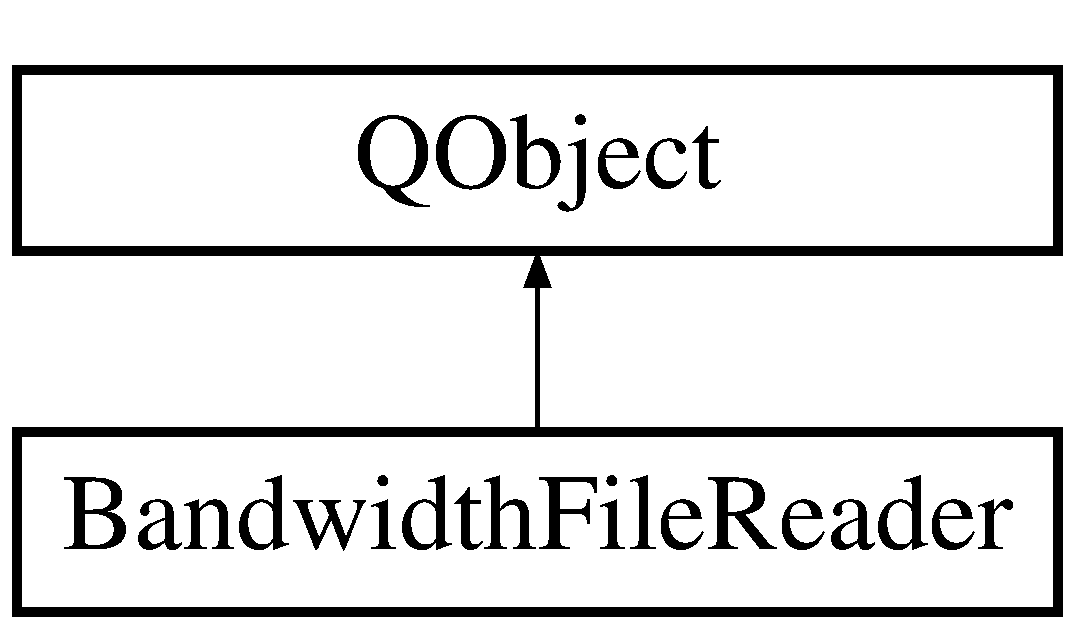
\includegraphics[height=2.000000cm]{classBandwidthFileReader}
\end{center}
\end{figure}
\subsection*{Public Slots}
\begin{DoxyCompactItemize}
\item 
void \hyperlink{classBandwidthFileReader_a49c0d54f1342d5e9c89645ef4a8d6d50}{read\-Loop} ()
\begin{DoxyCompactList}\small\item\em The read\-Loop slot. \end{DoxyCompactList}\end{DoxyCompactItemize}
\subsection*{Signals}
\begin{DoxyCompactItemize}
\item 
void \hyperlink{classBandwidthFileReader_abd0490c2362d76086fd6b2c741357a44}{new\-Bandwidth} (Q\-String bandwidth)
\begin{DoxyCompactList}\small\item\em Slot to signal a new bandwidth is available. \end{DoxyCompactList}\item 
void \hyperlink{classBandwidthFileReader_a1d2d50deda4271b620377958bf756d9f}{finished} ()
\begin{DoxyCompactList}\small\item\em Signal emitted when work has completed. \end{DoxyCompactList}\end{DoxyCompactItemize}
\subsection*{Public Member Functions}
\begin{DoxyCompactItemize}
\item 
\hyperlink{classBandwidthFileReader_a916d76632b3cb458331f86ec3101a4d4}{Bandwidth\-File\-Reader} (Q\-String \&filename)
\begin{DoxyCompactList}\small\item\em Explicit value contructor. \end{DoxyCompactList}\item 
\hyperlink{classBandwidthFileReader_a9ae6867549182c7bcf34718580bae864}{$\sim$\-Bandwidth\-File\-Reader} ()
\item 
void \hyperlink{classBandwidthFileReader_a0301d713d44225001bd87e7f423bd753}{set\-Ready\-Flag} (bool val)
\begin{DoxyCompactList}\small\item\em Set the value of the ready flag. \end{DoxyCompactList}\end{DoxyCompactItemize}


\subsection{Detailed Description}
A T\-E\-S\-T class to read a file that will contain bandwidth information. 

This class is used for testing purposes for reading a file that will contain information about available channel bandwidth. The class will open the file and read lines as they become available that will write the new value of the bandiwdth in Kbps. 

\subsection{Constructor \& Destructor Documentation}
\hypertarget{classBandwidthFileReader_a916d76632b3cb458331f86ec3101a4d4}{\index{Bandwidth\-File\-Reader@{Bandwidth\-File\-Reader}!Bandwidth\-File\-Reader@{Bandwidth\-File\-Reader}}
\index{Bandwidth\-File\-Reader@{Bandwidth\-File\-Reader}!BandwidthFileReader@{Bandwidth\-File\-Reader}}
\subsubsection[{Bandwidth\-File\-Reader}]{\setlength{\rightskip}{0pt plus 5cm}Bandwidth\-File\-Reader\-::\-Bandwidth\-File\-Reader (
\begin{DoxyParamCaption}
\item[{Q\-String \&}]{filename}
\end{DoxyParamCaption}
)}}\label{classBandwidthFileReader_a916d76632b3cb458331f86ec3101a4d4}


Explicit value contructor. 


\begin{DoxyParams}{Parameters}
{\em filename} & The name of the bandwidth information file. \\
\hline
\end{DoxyParams}

\begin{DoxyCode}
4                                                           :
5     m\_filereader(\hyperlink{classFileReaderUtility}{FileReaderUtility}())
6 \{
7     \textcolor{comment}{//Create the fifo and set the path}
8     QString fifo\_name(\hyperlink{Constants_8h_a5dcb1c9f587abfbe92034f35420f9ba4}{BWFILE\_PATH});
9     fifo\_name += filename;
10 
11     \textcolor{comment}{//Create the fifo}
12     \textcolor{keywordtype}{int} ready = mkfifo(fifo\_name.toStdString().c\_str(), S\_IRUSR | S\_IWUSR | S\_IRGRP | S\_IWGRP | S\_IROTH);
13 
14     \textcolor{comment}{//Set the ready flag}
15     \textcolor{keywordflow}{if}(ready == 0)
16     \{
17         \textcolor{comment}{//Set the file reader file}
18         m\_filereader.\hyperlink{classFileReaderUtility_a8d4984a9b7f18c589906d6e26956402b}{setFile}(fifo\_name);
19         m\_ready = \textcolor{keyword}{true};
20     \}
21     \textcolor{keywordflow}{else}
22         m\_ready = \textcolor{keyword}{false};
23 \}
\end{DoxyCode}
\hypertarget{classBandwidthFileReader_a9ae6867549182c7bcf34718580bae864}{\index{Bandwidth\-File\-Reader@{Bandwidth\-File\-Reader}!$\sim$\-Bandwidth\-File\-Reader@{$\sim$\-Bandwidth\-File\-Reader}}
\index{$\sim$\-Bandwidth\-File\-Reader@{$\sim$\-Bandwidth\-File\-Reader}!BandwidthFileReader@{Bandwidth\-File\-Reader}}
\subsubsection[{$\sim$\-Bandwidth\-File\-Reader}]{\setlength{\rightskip}{0pt plus 5cm}Bandwidth\-File\-Reader\-::$\sim$\-Bandwidth\-File\-Reader (
\begin{DoxyParamCaption}
{}
\end{DoxyParamCaption}
)}}\label{classBandwidthFileReader_a9ae6867549182c7bcf34718580bae864}

\begin{DoxyCode}
26 \{
27     \textcolor{comment}{//Destroy the fifo}
28     unlink(m\_filereader.\hyperlink{classFileReaderUtility_a9a871c01eeb7336d5d2cbc90d1550d3d}{getFile}().toStdString().c\_str());
29 \}
\end{DoxyCode}


\subsection{Member Function Documentation}
\hypertarget{classBandwidthFileReader_a1d2d50deda4271b620377958bf756d9f}{\index{Bandwidth\-File\-Reader@{Bandwidth\-File\-Reader}!finished@{finished}}
\index{finished@{finished}!BandwidthFileReader@{Bandwidth\-File\-Reader}}
\subsubsection[{finished}]{\setlength{\rightskip}{0pt plus 5cm}void Bandwidth\-File\-Reader\-::finished (
\begin{DoxyParamCaption}
{}
\end{DoxyParamCaption}
)\hspace{0.3cm}{\ttfamily [signal]}}}\label{classBandwidthFileReader_a1d2d50deda4271b620377958bf756d9f}


Signal emitted when work has completed. 

\hypertarget{classBandwidthFileReader_abd0490c2362d76086fd6b2c741357a44}{\index{Bandwidth\-File\-Reader@{Bandwidth\-File\-Reader}!new\-Bandwidth@{new\-Bandwidth}}
\index{new\-Bandwidth@{new\-Bandwidth}!BandwidthFileReader@{Bandwidth\-File\-Reader}}
\subsubsection[{new\-Bandwidth}]{\setlength{\rightskip}{0pt plus 5cm}void Bandwidth\-File\-Reader\-::new\-Bandwidth (
\begin{DoxyParamCaption}
\item[{Q\-String}]{bandwidth}
\end{DoxyParamCaption}
)\hspace{0.3cm}{\ttfamily [signal]}}}\label{classBandwidthFileReader_abd0490c2362d76086fd6b2c741357a44}


Slot to signal a new bandwidth is available. 


\begin{DoxyParams}{Parameters}
{\em bandwidth} & The new bandwidth. \\
\hline
\end{DoxyParams}
\hypertarget{classBandwidthFileReader_a49c0d54f1342d5e9c89645ef4a8d6d50}{\index{Bandwidth\-File\-Reader@{Bandwidth\-File\-Reader}!read\-Loop@{read\-Loop}}
\index{read\-Loop@{read\-Loop}!BandwidthFileReader@{Bandwidth\-File\-Reader}}
\subsubsection[{read\-Loop}]{\setlength{\rightskip}{0pt plus 5cm}void Bandwidth\-File\-Reader\-::read\-Loop (
\begin{DoxyParamCaption}
{}
\end{DoxyParamCaption}
)\hspace{0.3cm}{\ttfamily [slot]}}}\label{classBandwidthFileReader_a49c0d54f1342d5e9c89645ef4a8d6d50}


The read\-Loop slot. 

This function will continuously read the bandwidth information file until E\-O\-F is found or the ready flag is set to false. 
\begin{DoxyCode}
41 \{
42     \textcolor{comment}{//Loop while the ready flag is set}
43 
44     \textcolor{comment}{//Try to open the file}
45     \textcolor{keywordtype}{bool} isReady = m\_filereader.\hyperlink{classFileReaderUtility_a77c879620e0ddcc16e966649a73aa5c5}{open\_file}();
46 
47     m\_readymutex.lock();
48     this->m\_ready = isReady;
49     m\_readymutex.unlock();
50 
51     \textcolor{keywordflow}{while}(isReady)
52     \{
53         \textcolor{comment}{//Read another line}
54         QString line = m\_filereader.\hyperlink{classFileReaderUtility_ab41fc317ab5f175f61a15f1c2dff20ab}{readLine}();
55 
56         \textcolor{comment}{//If a null string}
57         \textcolor{keywordflow}{if}(!m\_filereader.\hyperlink{classFileReaderUtility_a0e8f0a86678ed4690758abad92d08520}{isOpen}() || line == \textcolor{stringliteral}{"-1"})
58         \{
59             \textcolor{comment}{//We've reached EOF}
60             m\_readymutex.lock();
61             this->m\_ready = \textcolor{keyword}{false};
62             m\_readymutex.unlock();
63         \}
64         \textcolor{keywordflow}{else}
65         \{
66             \textcolor{comment}{//Signal we have a new bandwidth}
67             \textcolor{keywordflow}{if}(line != \textcolor{stringliteral}{""})
68                 emit \hyperlink{classBandwidthFileReader_abd0490c2362d76086fd6b2c741357a44}{newBandwidth}(line);
69         \}
70 
71         \textcolor{comment}{//Set the new value of isReady}
72         \textcolor{comment}{//Lock the mutex}
73         m\_readymutex.lock();
74         \textcolor{comment}{//Set}
75         isReady = this->m\_ready;
76         \textcolor{comment}{//Unlock}
77         m\_readymutex.unlock();
78     \}
79 
80     m\_filereader.\hyperlink{classFileReaderUtility_ab8c0f909bc4d5325ad062a35451442a5}{close}();
81 
82     \textcolor{comment}{//Destroy the fifo}
83     unlink(m\_filereader.\hyperlink{classFileReaderUtility_a9a871c01eeb7336d5d2cbc90d1550d3d}{getFile}().toStdString().c\_str());
84 
85     \textcolor{comment}{//Finished}
86     emit \hyperlink{classBandwidthFileReader_a1d2d50deda4271b620377958bf756d9f}{finished}();
87 \}
\end{DoxyCode}
\hypertarget{classBandwidthFileReader_a0301d713d44225001bd87e7f423bd753}{\index{Bandwidth\-File\-Reader@{Bandwidth\-File\-Reader}!set\-Ready\-Flag@{set\-Ready\-Flag}}
\index{set\-Ready\-Flag@{set\-Ready\-Flag}!BandwidthFileReader@{Bandwidth\-File\-Reader}}
\subsubsection[{set\-Ready\-Flag}]{\setlength{\rightskip}{0pt plus 5cm}void Bandwidth\-File\-Reader\-::set\-Ready\-Flag (
\begin{DoxyParamCaption}
\item[{bool}]{val}
\end{DoxyParamCaption}
)}}\label{classBandwidthFileReader_a0301d713d44225001bd87e7f423bd753}


Set the value of the ready flag. 


\begin{DoxyParams}{Parameters}
{\em val} & The new value of the read flag. \\
\hline
\end{DoxyParams}

\begin{DoxyCode}
33 \{
34     m\_readymutex.lock();
35     this->m\_ready = val;
36     m\_readymutex.unlock();
37 \}
\end{DoxyCode}


The documentation for this class was generated from the following files\-:\begin{DoxyCompactItemize}
\item 
Util/\-File\-Util/\hyperlink{bandwidthfilereader_8h}{bandwidthfilereader.\-h}\item 
Util/\-File\-Util/\hyperlink{bandwidthfilereader_8cpp}{bandwidthfilereader.\-cpp}\end{DoxyCompactItemize}

\hypertarget{structbuffer__holder}{\section{buffer\-\_\-holder Struct Reference}
\label{structbuffer__holder}\index{buffer\-\_\-holder@{buffer\-\_\-holder}}
}
\subsection*{Public Member Functions}
\begin{DoxyCompactItemize}
\item 
\hyperlink{structbuffer__holder_aec91ad4dabc8db2a6cacac601b317857}{buffer\-\_\-holder} (void $\ast$data\-\_\-, void($\ast$deleter\-\_\-)(void $\ast$))
\item 
\hyperlink{structbuffer__holder_a43e10af0ca501bfa9bd1c2a012937876}{$\sim$buffer\-\_\-holder} ()
\item 
void $\ast$ \hyperlink{structbuffer__holder_add9b75027bdf15dee0e2dc88225d5b10}{release} ()
\end{DoxyCompactItemize}
\subsection*{Data Fields}
\begin{DoxyCompactItemize}
\item 
void $\ast$ \hyperlink{structbuffer__holder_a06c1e1004fac90848dfdb4fbc150cede}{data}
\item 
void($\ast$ \hyperlink{structbuffer__holder_a96e7067c68bc1f7a9ee7dd75c84f04e8}{deleter} )(void $\ast$)
\end{DoxyCompactItemize}


\subsection{Constructor \& Destructor Documentation}
\hypertarget{structbuffer__holder_aec91ad4dabc8db2a6cacac601b317857}{\index{buffer\-\_\-holder@{buffer\-\_\-holder}!buffer\-\_\-holder@{buffer\-\_\-holder}}
\index{buffer\-\_\-holder@{buffer\-\_\-holder}!buffer_holder@{buffer\-\_\-holder}}
\subsubsection[{buffer\-\_\-holder}]{\setlength{\rightskip}{0pt plus 5cm}buffer\-\_\-holder\-::buffer\-\_\-holder (
\begin{DoxyParamCaption}
\item[{void $\ast$}]{data\-\_\-, }
\item[{void($\ast$)(void $\ast$)}]{deleter\-\_\-}
\end{DoxyParamCaption}
)\hspace{0.3cm}{\ttfamily [inline]}}}\label{structbuffer__holder_aec91ad4dabc8db2a6cacac601b317857}

\begin{DoxyCode}
217                                                            : \hyperlink{structbuffer__holder_a06c1e1004fac90848dfdb4fbc150cede}{data}(data\_), 
      \hyperlink{structbuffer__holder_a96e7067c68bc1f7a9ee7dd75c84f04e8}{deleter}(deleter\_)
218         \{
219         \}
\end{DoxyCode}
\hypertarget{structbuffer__holder_a43e10af0ca501bfa9bd1c2a012937876}{\index{buffer\-\_\-holder@{buffer\-\_\-holder}!$\sim$buffer\-\_\-holder@{$\sim$buffer\-\_\-holder}}
\index{$\sim$buffer\-\_\-holder@{$\sim$buffer\-\_\-holder}!buffer_holder@{buffer\-\_\-holder}}
\subsubsection[{$\sim$buffer\-\_\-holder}]{\setlength{\rightskip}{0pt plus 5cm}buffer\-\_\-holder\-::$\sim$buffer\-\_\-holder (
\begin{DoxyParamCaption}
{}
\end{DoxyParamCaption}
)\hspace{0.3cm}{\ttfamily [inline]}}}\label{structbuffer__holder_a43e10af0ca501bfa9bd1c2a012937876}

\begin{DoxyCode}
222         \{
223             \textcolor{keywordflow}{if} (\hyperlink{structbuffer__holder_a06c1e1004fac90848dfdb4fbc150cede}{data}) \hyperlink{structbuffer__holder_a96e7067c68bc1f7a9ee7dd75c84f04e8}{deleter}(\hyperlink{structbuffer__holder_a06c1e1004fac90848dfdb4fbc150cede}{data});
224         \}
\end{DoxyCode}


\subsection{Member Function Documentation}
\hypertarget{structbuffer__holder_add9b75027bdf15dee0e2dc88225d5b10}{\index{buffer\-\_\-holder@{buffer\-\_\-holder}!release@{release}}
\index{release@{release}!buffer_holder@{buffer\-\_\-holder}}
\subsubsection[{release}]{\setlength{\rightskip}{0pt plus 5cm}void$\ast$ buffer\-\_\-holder\-::release (
\begin{DoxyParamCaption}
{}
\end{DoxyParamCaption}
)\hspace{0.3cm}{\ttfamily [inline]}}}\label{structbuffer__holder_add9b75027bdf15dee0e2dc88225d5b10}

\begin{DoxyCode}
227         \{
228             \textcolor{keywordtype}{void}* result = \hyperlink{structbuffer__holder_a06c1e1004fac90848dfdb4fbc150cede}{data};
229             \hyperlink{structbuffer__holder_a06c1e1004fac90848dfdb4fbc150cede}{data} = 0;
230             \textcolor{keywordflow}{return} result;
231         \}
\end{DoxyCode}


\subsection{Field Documentation}
\hypertarget{structbuffer__holder_a06c1e1004fac90848dfdb4fbc150cede}{\index{buffer\-\_\-holder@{buffer\-\_\-holder}!data@{data}}
\index{data@{data}!buffer_holder@{buffer\-\_\-holder}}
\subsubsection[{data}]{\setlength{\rightskip}{0pt plus 5cm}void$\ast$ buffer\-\_\-holder\-::data}}\label{structbuffer__holder_a06c1e1004fac90848dfdb4fbc150cede}
\hypertarget{structbuffer__holder_a96e7067c68bc1f7a9ee7dd75c84f04e8}{\index{buffer\-\_\-holder@{buffer\-\_\-holder}!deleter@{deleter}}
\index{deleter@{deleter}!buffer_holder@{buffer\-\_\-holder}}
\subsubsection[{deleter}]{\setlength{\rightskip}{0pt plus 5cm}void($\ast$ buffer\-\_\-holder\-::deleter)(void $\ast$)}}\label{structbuffer__holder_a96e7067c68bc1f7a9ee7dd75c84f04e8}


The documentation for this struct was generated from the following file\-:\begin{DoxyCompactItemize}
\item 
Third\-Party/pugixml/\hyperlink{pugixml_8cpp}{pugixml.\-cpp}\end{DoxyCompactItemize}

\hypertarget{classCamera}{\section{Camera Class Reference}
\label{classCamera}\index{Camera@{Camera}}
}


The \hyperlink{classCamera}{Camera} class.  




{\ttfamily \#include $<$camera.\-h$>$}

Inheritance diagram for Camera\-:\begin{figure}[H]
\begin{center}
\leavevmode
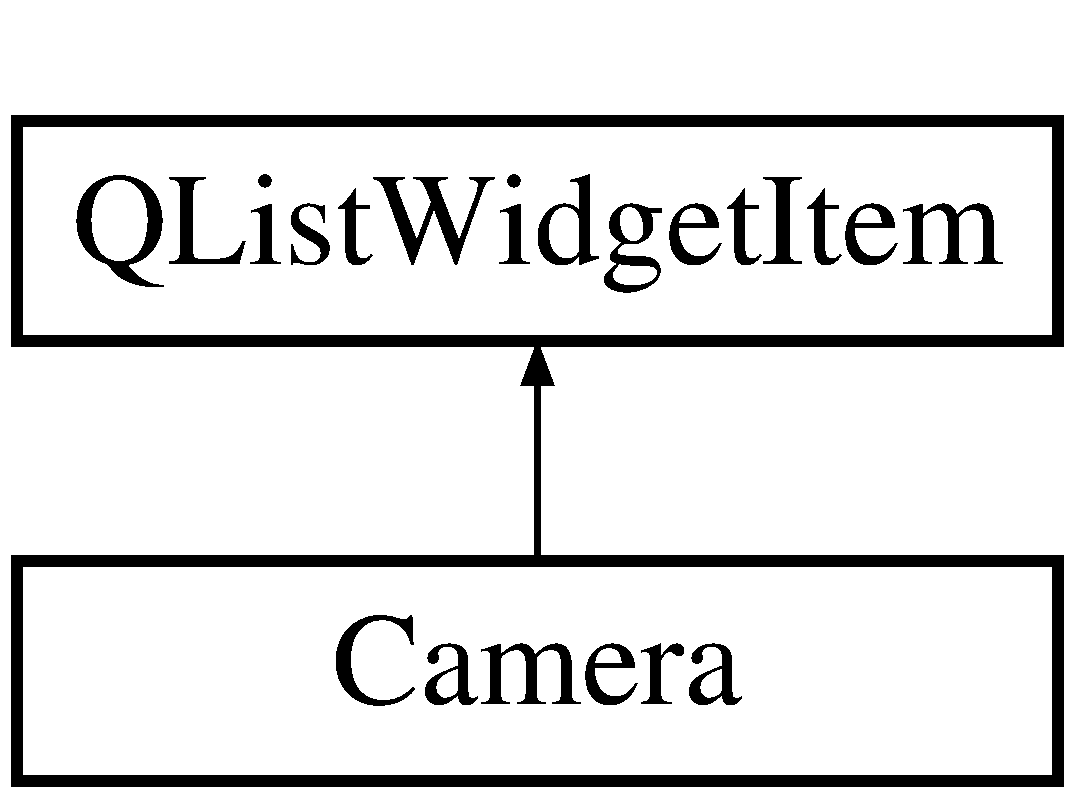
\includegraphics[height=2.000000cm]{classCamera}
\end{center}
\end{figure}
\subsection*{Public Member Functions}
\begin{DoxyCompactItemize}
\item 
\hyperlink{classCamera_a01f94c3543f56ede7af49dc778f19331}{Camera} ()
\begin{DoxyCompactList}\small\item\em Default value constructor. \end{DoxyCompactList}\item 
\hyperlink{classCamera_a5a4ceda635ed01219348078adddb141b}{Camera} (Q\-String \&\hyperlink{classCamera_a5763757e8d6adb6437dde2502072a3b1}{name}, \hyperlink{classAddress}{Address} \&address, \hyperlink{camera_8h_a10395294162cb49637e9c8f6efdb10ea}{Camera\-Content\-Type} content\-\_\-type)
\begin{DoxyCompactList}\small\item\em Explicit value constructor. \end{DoxyCompactList}\item 
Q\-String \hyperlink{classCamera_a5763757e8d6adb6437dde2502072a3b1}{name} () const 
\begin{DoxyCompactList}\small\item\em Accessor for the camera name field. \end{DoxyCompactList}\item 
void \hyperlink{classCamera_a4f009de64587caa5e2a91a2cdd18fd32}{set\-Name} (const Q\-String \&\hyperlink{classCamera_a5763757e8d6adb6437dde2502072a3b1}{name})
\begin{DoxyCompactList}\small\item\em Mutator for the camera name field. \end{DoxyCompactList}\item 
\hyperlink{classAddress}{Address} \hyperlink{classCamera_aa93654bec9b65adfb95e192ac9c71e80}{server\-\_\-address} () const 
\begin{DoxyCompactList}\small\item\em Accessor for the server address field. \end{DoxyCompactList}\item 
void \hyperlink{classCamera_a678d67d964307ffc9e323d74c7a28ca1}{set\-Server\-\_\-address} (const \hyperlink{classAddress}{Address} \&\hyperlink{classCamera_aa93654bec9b65adfb95e192ac9c71e80}{server\-\_\-address})
\begin{DoxyCompactList}\small\item\em Mutator for the server address field. \end{DoxyCompactList}\item 
bool \hyperlink{classCamera_a1b7b69303090eb7557713a6dda3d3de4}{operator==} (const \hyperlink{classCamera}{Camera} \&rhs)
\end{DoxyCompactItemize}


\subsection{Detailed Description}
The \hyperlink{classCamera}{Camera} class. 

This class describes a camera that can stream video to the client. It inherits from the Q\-List\-Widget\-Item class in order to facilitate its use in list boxes. 

\subsection{Constructor \& Destructor Documentation}
\hypertarget{classCamera_a01f94c3543f56ede7af49dc778f19331}{\index{Camera@{Camera}!Camera@{Camera}}
\index{Camera@{Camera}!Camera@{Camera}}
\subsubsection[{Camera}]{\setlength{\rightskip}{0pt plus 5cm}Camera\-::\-Camera (
\begin{DoxyParamCaption}
{}
\end{DoxyParamCaption}
)}}\label{classCamera_a01f94c3543f56ede7af49dc778f19331}


Default value constructor. 


\begin{DoxyCode}
5 \{
6 \}
\end{DoxyCode}
\hypertarget{classCamera_a5a4ceda635ed01219348078adddb141b}{\index{Camera@{Camera}!Camera@{Camera}}
\index{Camera@{Camera}!Camera@{Camera}}
\subsubsection[{Camera}]{\setlength{\rightskip}{0pt plus 5cm}Camera\-::\-Camera (
\begin{DoxyParamCaption}
\item[{Q\-String \&}]{name, }
\item[{{\bf Address} \&}]{address, }
\item[{{\bf Camera\-Content\-Type}}]{content\-\_\-type}
\end{DoxyParamCaption}
)}}\label{classCamera_a5a4ceda635ed01219348078adddb141b}


Explicit value constructor. 


\begin{DoxyParams}{Parameters}
{\em name} & The name of this camera. \\
\hline
{\em address} & The address of the server to which this camera refers to. \\
\hline
\end{DoxyParams}

\begin{DoxyCode}
8                                                                               :
9     QListWidgetItem(\hyperlink{classCamera_a5763757e8d6adb6437dde2502072a3b1}{name}),
10     m\_name(\hyperlink{classCamera_a5763757e8d6adb6437dde2502072a3b1}{name}),
11     m\_server\_address(address),
12     m\_content\_type(content\_type)
13 \{
14 \}
\end{DoxyCode}


\subsection{Member Function Documentation}
\hypertarget{classCamera_a5763757e8d6adb6437dde2502072a3b1}{\index{Camera@{Camera}!name@{name}}
\index{name@{name}!Camera@{Camera}}
\subsubsection[{name}]{\setlength{\rightskip}{0pt plus 5cm}Q\-String Camera\-::name (
\begin{DoxyParamCaption}
{}
\end{DoxyParamCaption}
) const}}\label{classCamera_a5763757e8d6adb6437dde2502072a3b1}


Accessor for the camera name field. 

\begin{DoxyReturn}{Returns}
The name of the camera. 
\end{DoxyReturn}

\begin{DoxyCode}
33 \{
34     \textcolor{keywordflow}{return} m\_name;
35 \}
\end{DoxyCode}
\hypertarget{classCamera_a1b7b69303090eb7557713a6dda3d3de4}{\index{Camera@{Camera}!operator==@{operator==}}
\index{operator==@{operator==}!Camera@{Camera}}
\subsubsection[{operator==}]{\setlength{\rightskip}{0pt plus 5cm}bool Camera\-::operator== (
\begin{DoxyParamCaption}
\item[{const {\bf Camera} \&}]{rhs}
\end{DoxyParamCaption}
)}}\label{classCamera_a1b7b69303090eb7557713a6dda3d3de4}

\begin{DoxyCode}
28 \{
29     \textcolor{keywordflow}{return} (this->\hyperlink{classCamera_a5763757e8d6adb6437dde2502072a3b1}{name}() == rhs.\hyperlink{classCamera_a5763757e8d6adb6437dde2502072a3b1}{name}() && this->\hyperlink{classCamera_aa93654bec9b65adfb95e192ac9c71e80}{server\_address}() == rhs.
      \hyperlink{classCamera_aa93654bec9b65adfb95e192ac9c71e80}{server\_address}());
30 \}
\end{DoxyCode}
\hypertarget{classCamera_aa93654bec9b65adfb95e192ac9c71e80}{\index{Camera@{Camera}!server\-\_\-address@{server\-\_\-address}}
\index{server\-\_\-address@{server\-\_\-address}!Camera@{Camera}}
\subsubsection[{server\-\_\-address}]{\setlength{\rightskip}{0pt plus 5cm}{\bf Address} Camera\-::server\-\_\-address (
\begin{DoxyParamCaption}
{}
\end{DoxyParamCaption}
) const}}\label{classCamera_aa93654bec9b65adfb95e192ac9c71e80}


Accessor for the server address field. 

\begin{DoxyReturn}{Returns}
The address of this camera's server. 
\end{DoxyReturn}

\begin{DoxyCode}
17 \{
18     \textcolor{keywordflow}{return} m\_server\_address;
19 \}
\end{DoxyCode}
\hypertarget{classCamera_a4f009de64587caa5e2a91a2cdd18fd32}{\index{Camera@{Camera}!set\-Name@{set\-Name}}
\index{set\-Name@{set\-Name}!Camera@{Camera}}
\subsubsection[{set\-Name}]{\setlength{\rightskip}{0pt plus 5cm}void Camera\-::set\-Name (
\begin{DoxyParamCaption}
\item[{const Q\-String \&}]{name}
\end{DoxyParamCaption}
)}}\label{classCamera_a4f009de64587caa5e2a91a2cdd18fd32}


Mutator for the camera name field. 


\begin{DoxyParams}{Parameters}
{\em name} & The new camera name. \\
\hline
\end{DoxyParams}

\begin{DoxyCode}
38 \{
39     m\_name = \hyperlink{classCamera_a5763757e8d6adb6437dde2502072a3b1}{name};
40     this->setText(\hyperlink{classCamera_a5763757e8d6adb6437dde2502072a3b1}{name});
41 \}
\end{DoxyCode}
\hypertarget{classCamera_a678d67d964307ffc9e323d74c7a28ca1}{\index{Camera@{Camera}!set\-Server\-\_\-address@{set\-Server\-\_\-address}}
\index{set\-Server\-\_\-address@{set\-Server\-\_\-address}!Camera@{Camera}}
\subsubsection[{set\-Server\-\_\-address}]{\setlength{\rightskip}{0pt plus 5cm}void Camera\-::set\-Server\-\_\-address (
\begin{DoxyParamCaption}
\item[{const {\bf Address} \&}]{server\-\_\-address}
\end{DoxyParamCaption}
)}}\label{classCamera_a678d67d964307ffc9e323d74c7a28ca1}


Mutator for the server address field. 


\begin{DoxyParams}{Parameters}
{\em server\-\_\-address} & The new address of the server. \\
\hline
\end{DoxyParams}

\begin{DoxyCode}
22 \{
23     m\_server\_address = \hyperlink{classCamera_aa93654bec9b65adfb95e192ac9c71e80}{server\_address};
24 \}
\end{DoxyCode}


The documentation for this class was generated from the following files\-:\begin{DoxyCompactItemize}
\item 
Types/\hyperlink{camera_8h}{camera.\-h}\item 
Types/\hyperlink{camera_8cpp}{camera.\-cpp}\end{DoxyCompactItemize}

\hypertarget{classCameraListFileUtil}{\section{Camera\-List\-File\-Util Class Reference}
\label{classCameraListFileUtil}\index{Camera\-List\-File\-Util@{Camera\-List\-File\-Util}}
}


An X\-M\-L file reading utility.  




{\ttfamily \#include $<$cameralistfileutil.\-h$>$}

\subsection*{Public Member Functions}
\begin{DoxyCompactItemize}
\item 
\hyperlink{classCameraListFileUtil_a8966248618d4fbd76c573dfaf009f42a}{Camera\-List\-File\-Util} ()
\begin{DoxyCompactList}\small\item\em Default value constructor. \end{DoxyCompactList}\item 
bool \hyperlink{classCameraListFileUtil_abb70006319c1301e47e02bd17d2098e2}{load\-Document} (Q\-String \&filename)
\begin{DoxyCompactList}\small\item\em Load the xml document. \end{DoxyCompactList}\item 
\hyperlink{camera_8h_a4e5cc6bdc5723a4d61f3aac69dbb083a}{Camera\-List} \hyperlink{classCameraListFileUtil_a8ea7a7091551688c46f5077d2fe632e9}{get\-Camera\-List} ()
\begin{DoxyCompactList}\small\item\em Get the camera list. \end{DoxyCompactList}\end{DoxyCompactItemize}


\subsection{Detailed Description}
An X\-M\-L file reading utility. 

This class defines a utility for reading and writing an xml configuration file containing a list of saved camera servers. 

\subsection{Constructor \& Destructor Documentation}
\hypertarget{classCameraListFileUtil_a8966248618d4fbd76c573dfaf009f42a}{\index{Camera\-List\-File\-Util@{Camera\-List\-File\-Util}!Camera\-List\-File\-Util@{Camera\-List\-File\-Util}}
\index{Camera\-List\-File\-Util@{Camera\-List\-File\-Util}!CameraListFileUtil@{Camera\-List\-File\-Util}}
\subsubsection[{Camera\-List\-File\-Util}]{\setlength{\rightskip}{0pt plus 5cm}Camera\-List\-File\-Util\-::\-Camera\-List\-File\-Util (
\begin{DoxyParamCaption}
{}
\end{DoxyParamCaption}
)}}\label{classCameraListFileUtil_a8966248618d4fbd76c573dfaf009f42a}


Default value constructor. 


\begin{DoxyCode}
5                                        :
6     m\_is\_loaded(\textcolor{keyword}{false}),
7     m\_open\_document(\textcolor{stringliteral}{""})
8 \{
9 \}
\end{DoxyCode}


\subsection{Member Function Documentation}
\hypertarget{classCameraListFileUtil_a8ea7a7091551688c46f5077d2fe632e9}{\index{Camera\-List\-File\-Util@{Camera\-List\-File\-Util}!get\-Camera\-List@{get\-Camera\-List}}
\index{get\-Camera\-List@{get\-Camera\-List}!CameraListFileUtil@{Camera\-List\-File\-Util}}
\subsubsection[{get\-Camera\-List}]{\setlength{\rightskip}{0pt plus 5cm}{\bf Camera\-List} Camera\-List\-File\-Util\-::get\-Camera\-List (
\begin{DoxyParamCaption}
{}
\end{DoxyParamCaption}
)}}\label{classCameraListFileUtil_a8ea7a7091551688c46f5077d2fe632e9}


Get the camera list. 

Parses the loaded xml document and returns a list of cameras. \begin{DoxyReturn}{Returns}
A list of cameras specified by the X\-M\-L document. 
\end{DoxyReturn}

\begin{DoxyCode}
38 \{
39     \hyperlink{camera_8h_a4e5cc6bdc5723a4d61f3aac69dbb083a}{CameraList} cameras;
40 
41     \textcolor{comment}{//See if document is loaded}
42     \textcolor{keywordflow}{if}(!m\_is\_loaded)
43         \textcolor{keywordflow}{return} cameras;
44 
45     \textcolor{comment}{//Parse the XML}
46 
47     \textcolor{comment}{//Load all cameras}
48     \hyperlink{classpugi_1_1xml__node}{xml\_node} cams = m\_root.\hyperlink{classpugi_1_1xml__node_af3aa192b114a289640110c9e4da020ca}{child}(\textcolor{stringliteral}{"cameraList"}).\hyperlink{classpugi_1_1xml__node_af3aa192b114a289640110c9e4da020ca}{child}(\textcolor{stringliteral}{"camera"});
49 
50     \textcolor{comment}{//Iterate through all cameras}
51     \textcolor{keywordflow}{for}(\hyperlink{classpugi_1_1xml__node}{xml\_node} cam = cams; cam; cam = cam.\hyperlink{classpugi_1_1xml__node_a713159ab981fb3f0a325434106dc94f5}{next\_sibling}())
52     \{
53         \textcolor{comment}{//NOTE --- RELYING ON THE UI TO DELETE ALLOCATED RESOURCES}
54         \hyperlink{classCamera}{Camera} *next\_camera = \textcolor{keyword}{new} \hyperlink{classCamera}{Camera}();
55         \textcolor{comment}{//Get the name}
56         \hyperlink{classpugi_1_1xml__attribute}{xml\_attribute} name = cam.attribute(\textcolor{stringliteral}{"name"});
57         next\_camera->\hyperlink{classCamera_a4f009de64587caa5e2a91a2cdd18fd32}{setName}(QString(name.\hyperlink{classpugi_1_1xml__attribute_a583f470d768f5f8a4df0ebb2e016a88d}{as\_string}()));
58 
59 
60 
61         \textcolor{comment}{//Get the address}
62         \hyperlink{classAddress}{Address} next\_addr;
63         \hyperlink{classpugi_1_1xml__node}{xml\_node} addr = cam.\hyperlink{classpugi_1_1xml__node_af3aa192b114a289640110c9e4da020ca}{child}(\textcolor{stringliteral}{"address"});
64         \hyperlink{classpugi_1_1xml__attribute}{xml\_attribute} port = addr.\hyperlink{classpugi_1_1xml__node_a19fc1a285c0f751f52c0e151a727de97}{attribute}(\textcolor{stringliteral}{"port"});
65         next\_addr.\hyperlink{classAddress_a43ba5f8001b7e729b83b1b9299294495}{setAddress}(std::string(addr.\hyperlink{classpugi_1_1xml__node_aafe1c1c7cd27f3c9c758b517abc7886a}{text}().\hyperlink{classpugi_1_1xml__text_ac817e480d7ab09b3c6390622423a701b}{as\_string}()));
66         next\_addr.\hyperlink{classAddress_ad73c29200f7d63641e48ebfc16efaf75}{setPort}(port.\hyperlink{classpugi_1_1xml__attribute_afe009e964b9cec96c77495ef1ae6d91f}{as\_int}());
67 
68         next\_camera->\hyperlink{classCamera_a678d67d964307ffc9e323d74c7a28ca1}{setServer\_address}(next\_addr);
69         \textcolor{comment}{//Get the content type}
70         \hyperlink{classpugi_1_1xml__node}{xml\_node} content\_type = cam.\hyperlink{classpugi_1_1xml__node_af3aa192b114a289640110c9e4da020ca}{child}(\textcolor{stringliteral}{"contentType"});
71         next\_camera->\hyperlink{classCamera_a1277a5aceff1a947a5a048b8edacd1cf}{setContent\_type}((\hyperlink{camera_8h_a10395294162cb49637e9c8f6efdb10ea}{CameraContentType})content\_type.
      \hyperlink{classpugi_1_1xml__node_a19fc1a285c0f751f52c0e151a727de97}{attribute}(\textcolor{stringliteral}{"enum"}).\hyperlink{classpugi_1_1xml__attribute_afe009e964b9cec96c77495ef1ae6d91f}{as\_int}());
72 
73         \textcolor{comment}{//Add to camera list}
74         cameras.push\_front(next\_camera);
75     \}
76 
77     \textcolor{keywordflow}{return} cameras;
78 \}
\end{DoxyCode}
\hypertarget{classCameraListFileUtil_abb70006319c1301e47e02bd17d2098e2}{\index{Camera\-List\-File\-Util@{Camera\-List\-File\-Util}!load\-Document@{load\-Document}}
\index{load\-Document@{load\-Document}!CameraListFileUtil@{Camera\-List\-File\-Util}}
\subsubsection[{load\-Document}]{\setlength{\rightskip}{0pt plus 5cm}bool Camera\-List\-File\-Util\-::load\-Document (
\begin{DoxyParamCaption}
\item[{Q\-String \&}]{filename}
\end{DoxyParamCaption}
)}}\label{classCameraListFileUtil_abb70006319c1301e47e02bd17d2098e2}


Load the xml document. 

This function will load the xml document into the pugixml backend. 
\begin{DoxyParams}{Parameters}
{\em filename} & The name of the xml file to load. \\
\hline
\end{DoxyParams}
\begin{DoxyReturn}{Returns}
True if the document loaded, false otherwise. 
\end{DoxyReturn}

\begin{DoxyCode}
13 \{
14     \textcolor{keywordtype}{bool} is\_loaded = \textcolor{keyword}{false};
15 
16     \textcolor{comment}{//Load the file}
17     \hyperlink{structpugi_1_1xml__parse__result}{xml\_parse\_result} result = m\_root.\hyperlink{classpugi_1_1xml__document_aad350209a4a91589fbd7e8cdaf79e010}{load\_file}(filename.toStdString().c\_str());
18 
19     \textcolor{keywordflow}{if}(result)
20     \{
21         \textcolor{comment}{//Success}
22         is\_loaded = \textcolor{keyword}{true};
23         this->m\_is\_loaded = \textcolor{keyword}{true};
24 
25         this->m\_open\_document = filename;
26     \}
27     \textcolor{keywordflow}{else}
28     \{
29         \hyperlink{Log_8h_a1a242c34c5066fb0c62d909f22d3716d}{L\_ERROR}() << \textcolor{stringliteral}{"Unable to load XML file: "} << filename;
30     \}
31 
32     \textcolor{keywordflow}{return} is\_loaded;
33 
34 \}
\end{DoxyCode}


The documentation for this class was generated from the following files\-:\begin{DoxyCompactItemize}
\item 
Util/\-File\-Util/\hyperlink{cameralistfileutil_8h}{cameralistfileutil.\-h}\item 
Util/\-File\-Util/\hyperlink{cameralistfileutil_8cpp}{cameralistfileutil.\-cpp}\end{DoxyCompactItemize}

\hypertarget{classControlCenter}{\section{Control\-Center Class Reference}
\label{classControlCenter}\index{Control\-Center@{Control\-Center}}
}


{\ttfamily \#include $<$controlcenter.\-h$>$}

Inheritance diagram for Control\-Center\-:\begin{figure}[H]
\begin{center}
\leavevmode
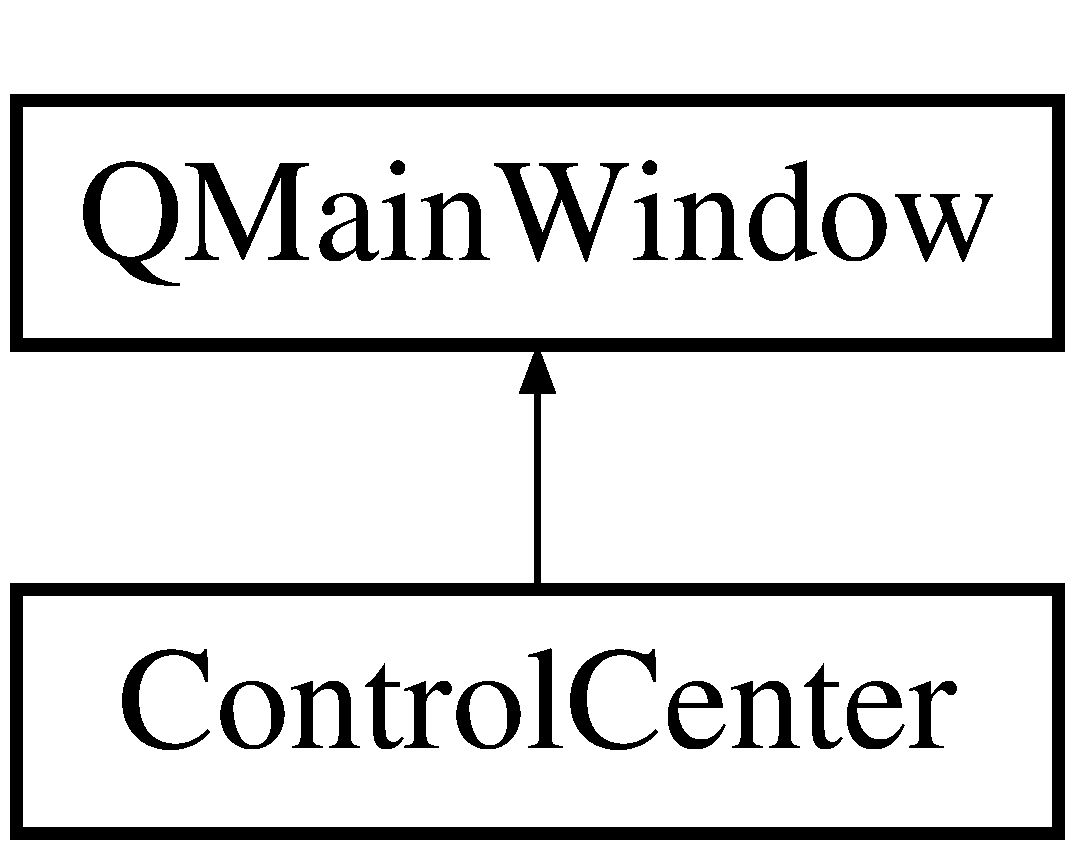
\includegraphics[height=2.000000cm]{classControlCenter}
\end{center}
\end{figure}
\subsection*{Public Member Functions}
\begin{DoxyCompactItemize}
\item 
\hyperlink{classControlCenter_aba3b5aafd3a4ee5c611d134b5d28d353}{Control\-Center} (\hyperlink{controlcenter_8h_aa96d2479f78139aaa02437fb3ece427d}{Camera\-List} cameras, Q\-Widget $\ast$parent=0)
\item 
\hyperlink{classControlCenter_a9ac145ced26cf2002a9d12c4c20bdc75}{$\sim$\-Control\-Center} ()
\end{DoxyCompactItemize}


\subsection{Constructor \& Destructor Documentation}
\hypertarget{classControlCenter_aba3b5aafd3a4ee5c611d134b5d28d353}{\index{Control\-Center@{Control\-Center}!Control\-Center@{Control\-Center}}
\index{Control\-Center@{Control\-Center}!ControlCenter@{Control\-Center}}
\subsubsection[{Control\-Center}]{\setlength{\rightskip}{0pt plus 5cm}Control\-Center\-::\-Control\-Center (
\begin{DoxyParamCaption}
\item[{{\bf Camera\-List}}]{cameras, }
\item[{Q\-Widget $\ast$}]{parent = {\ttfamily 0}}
\end{DoxyParamCaption}
)\hspace{0.3cm}{\ttfamily [explicit]}}}\label{classControlCenter_aba3b5aafd3a4ee5c611d134b5d28d353}

\begin{DoxyCode}
6                                                                 :
7     QMainWindow(parent),
8     ui(\textcolor{keyword}{new} Ui::ControlCenter)
9 \{
10     ui->setupUi(\textcolor{keyword}{this});
11     this->setFixedSize(this->size());
12 
13     \textcolor{comment}{//c = new Camera(q, a);}
14 
15     this->addCameras(cameras);
16 
17     connect(ui->actionQuit, SIGNAL(triggered()), \textcolor{keyword}{this}, SLOT(quitActionClicked()));
18     QShortcut *quitHotkey = \textcolor{keyword}{new} QShortcut(QKeySequence(\textcolor{stringliteral}{"Ctrl+Q"}), \textcolor{keyword}{this});
19     connect(quitHotkey, SIGNAL(activated()), \textcolor{keyword}{this}, SLOT(quitActionClicked()));
20 
21     \textcolor{comment}{//Set up demuxer test}
22     m\_ffmpeg = \textcolor{keyword}{new} \hyperlink{classFFMPEGWrapper}{FFMPEGWrapper}(39082);
23     m\_ffmpeg\_thread = \textcolor{keyword}{new} QThread(\textcolor{keyword}{this});
24     m\_ffmpeg->moveToThread(m\_ffmpeg\_thread);
25     connect(m\_ffmpeg\_thread, SIGNAL(started()), m\_ffmpeg, SLOT(demux()));
26     connect(m\_ffmpeg, SIGNAL(finished()), m\_ffmpeg\_thread, SLOT(quit()));
27 
28 \}
\end{DoxyCode}
\hypertarget{classControlCenter_a9ac145ced26cf2002a9d12c4c20bdc75}{\index{Control\-Center@{Control\-Center}!$\sim$\-Control\-Center@{$\sim$\-Control\-Center}}
\index{$\sim$\-Control\-Center@{$\sim$\-Control\-Center}!ControlCenter@{Control\-Center}}
\subsubsection[{$\sim$\-Control\-Center}]{\setlength{\rightskip}{0pt plus 5cm}Control\-Center\-::$\sim$\-Control\-Center (
\begin{DoxyParamCaption}
{}
\end{DoxyParamCaption}
)}}\label{classControlCenter_a9ac145ced26cf2002a9d12c4c20bdc75}

\begin{DoxyCode}
31 \{
32     \textcolor{keyword}{delete} ui;
33 
34 \}
\end{DoxyCode}


The documentation for this class was generated from the following files\-:\begin{DoxyCompactItemize}
\item 
\hyperlink{controlcenter_8h}{controlcenter.\-h}\item 
\hyperlink{controlcenter_8cpp}{controlcenter.\-cpp}\end{DoxyCompactItemize}

\hypertarget{classDemuxer}{\section{Demuxer Class Reference}
\label{classDemuxer}\index{Demuxer@{Demuxer}}
}


{\ttfamily \#include $<$demuxer.\-h$>$}

Inheritance diagram for Demuxer\-:\begin{figure}[H]
\begin{center}
\leavevmode
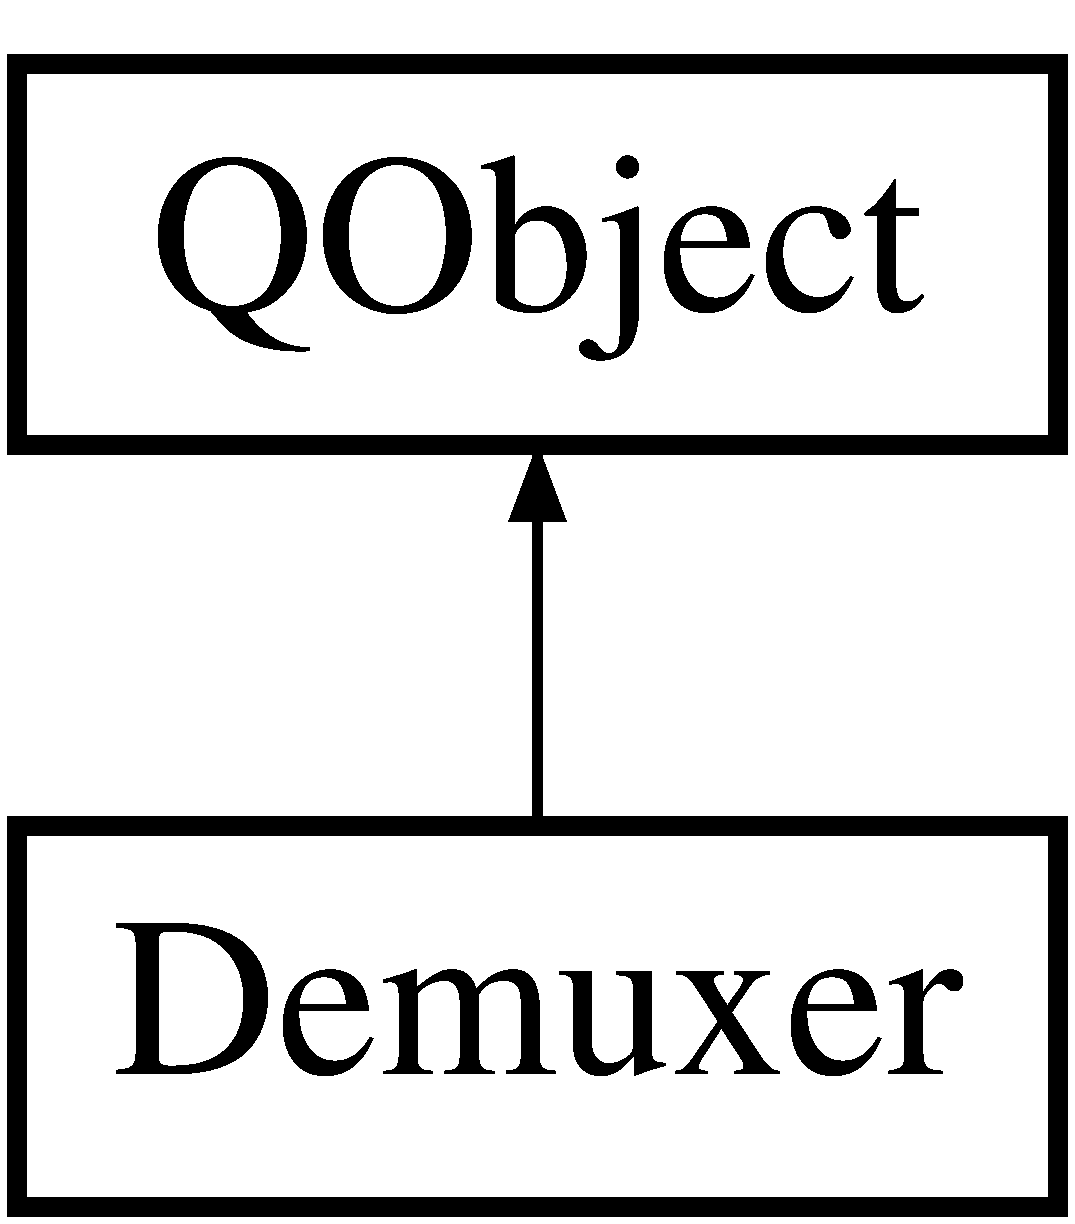
\includegraphics[height=2.000000cm]{classDemuxer}
\end{center}
\end{figure}
\subsection*{Public Slots}
\begin{DoxyCompactItemize}
\item 
void \hyperlink{classDemuxer_a95c38d118f61403a2828da35afc39c5f}{demux} ()
\end{DoxyCompactItemize}
\subsection*{Signals}
\begin{DoxyCompactItemize}
\item 
void \hyperlink{classDemuxer_a62e1d551bc7e73a9fa23587b1960b92f}{finished} ()
\item 
void \hyperlink{classDemuxer_a0a8254e06b4450d65428e9d1f641c8cd}{new\-Image} (Q\-Image $\ast$)
\end{DoxyCompactItemize}
\subsection*{Public Member Functions}
\begin{DoxyCompactItemize}
\item 
\hyperlink{classDemuxer_a266feb24cfea87bee1883b480694478d}{Demuxer} (Q\-String \hyperlink{classDemuxer_a4bd7bbc10d0c5356ac541b5f168fde93}{fifo}, Q\-Object $\ast$parent=0)
\item 
Q\-String \hyperlink{classDemuxer_a4bd7bbc10d0c5356ac541b5f168fde93}{fifo} () const 
\item 
void \hyperlink{classDemuxer_a92ca6dbf8971a34ecac0e6b671c588ed}{set\-Fifo} (const Q\-String \&\hyperlink{classDemuxer_a4bd7bbc10d0c5356ac541b5f168fde93}{fifo})
\end{DoxyCompactItemize}


\subsection{Constructor \& Destructor Documentation}
\hypertarget{classDemuxer_a266feb24cfea87bee1883b480694478d}{\index{Demuxer@{Demuxer}!Demuxer@{Demuxer}}
\index{Demuxer@{Demuxer}!Demuxer@{Demuxer}}
\subsubsection[{Demuxer}]{\setlength{\rightskip}{0pt plus 5cm}Demuxer\-::\-Demuxer (
\begin{DoxyParamCaption}
\item[{Q\-String}]{fifo, }
\item[{Q\-Object $\ast$}]{parent = {\ttfamily 0}}
\end{DoxyParamCaption}
)\hspace{0.3cm}{\ttfamily [explicit]}}}\label{classDemuxer_a266feb24cfea87bee1883b480694478d}

\begin{DoxyCode}
4                                               :
5     QObject(parent),
6     m\_fifo(\hyperlink{classDemuxer_a4bd7bbc10d0c5356ac541b5f168fde93}{fifo}),
7     video\_frame\_count(0),
8     destination\_data(\{NULL\})
\end{DoxyCode}


\subsection{Member Function Documentation}
\hypertarget{classDemuxer_a95c38d118f61403a2828da35afc39c5f}{\index{Demuxer@{Demuxer}!demux@{demux}}
\index{demux@{demux}!Demuxer@{Demuxer}}
\subsubsection[{demux}]{\setlength{\rightskip}{0pt plus 5cm}void Demuxer\-::demux (
\begin{DoxyParamCaption}
{}
\end{DoxyParamCaption}
)\hspace{0.3cm}{\ttfamily [slot]}}}\label{classDemuxer_a95c38d118f61403a2828da35afc39c5f}
\hypertarget{classDemuxer_a4bd7bbc10d0c5356ac541b5f168fde93}{\index{Demuxer@{Demuxer}!fifo@{fifo}}
\index{fifo@{fifo}!Demuxer@{Demuxer}}
\subsubsection[{fifo}]{\setlength{\rightskip}{0pt plus 5cm}Q\-String Demuxer\-::fifo (
\begin{DoxyParamCaption}
{}
\end{DoxyParamCaption}
) const}}\label{classDemuxer_a4bd7bbc10d0c5356ac541b5f168fde93}
\hypertarget{classDemuxer_a62e1d551bc7e73a9fa23587b1960b92f}{\index{Demuxer@{Demuxer}!finished@{finished}}
\index{finished@{finished}!Demuxer@{Demuxer}}
\subsubsection[{finished}]{\setlength{\rightskip}{0pt plus 5cm}void Demuxer\-::finished (
\begin{DoxyParamCaption}
{}
\end{DoxyParamCaption}
)\hspace{0.3cm}{\ttfamily [signal]}}}\label{classDemuxer_a62e1d551bc7e73a9fa23587b1960b92f}
\hypertarget{classDemuxer_a0a8254e06b4450d65428e9d1f641c8cd}{\index{Demuxer@{Demuxer}!new\-Image@{new\-Image}}
\index{new\-Image@{new\-Image}!Demuxer@{Demuxer}}
\subsubsection[{new\-Image}]{\setlength{\rightskip}{0pt plus 5cm}void Demuxer\-::new\-Image (
\begin{DoxyParamCaption}
\item[{Q\-Image $\ast$}]{}
\end{DoxyParamCaption}
)\hspace{0.3cm}{\ttfamily [signal]}}}\label{classDemuxer_a0a8254e06b4450d65428e9d1f641c8cd}
\hypertarget{classDemuxer_a92ca6dbf8971a34ecac0e6b671c588ed}{\index{Demuxer@{Demuxer}!set\-Fifo@{set\-Fifo}}
\index{set\-Fifo@{set\-Fifo}!Demuxer@{Demuxer}}
\subsubsection[{set\-Fifo}]{\setlength{\rightskip}{0pt plus 5cm}void Demuxer\-::set\-Fifo (
\begin{DoxyParamCaption}
\item[{const Q\-String \&}]{fifo}
\end{DoxyParamCaption}
)}}\label{classDemuxer_a92ca6dbf8971a34ecac0e6b671c588ed}


The documentation for this class was generated from the following files\-:\begin{DoxyCompactItemize}
\item 
Video/\hyperlink{demuxer_8h}{demuxer.\-h}\item 
Video/\hyperlink{demuxer_8cpp}{demuxer.\-cpp}\end{DoxyCompactItemize}

\hypertarget{structdocument__order__comparator}{\section{document\-\_\-order\-\_\-comparator Struct Reference}
\label{structdocument__order__comparator}\index{document\-\_\-order\-\_\-comparator@{document\-\_\-order\-\_\-comparator}}
}
\subsection*{Public Member Functions}
\begin{DoxyCompactItemize}
\item 
bool \hyperlink{structdocument__order__comparator_a11e471cbfa426bc9e48844c1db1a190e}{operator()} (const xpath\-\_\-node \&lhs, const xpath\-\_\-node \&rhs) const 
\end{DoxyCompactItemize}


\subsection{Member Function Documentation}
\hypertarget{structdocument__order__comparator_a11e471cbfa426bc9e48844c1db1a190e}{\index{document\-\_\-order\-\_\-comparator@{document\-\_\-order\-\_\-comparator}!operator()@{operator()}}
\index{operator()@{operator()}!document_order_comparator@{document\-\_\-order\-\_\-comparator}}
\subsubsection[{operator()}]{\setlength{\rightskip}{0pt plus 5cm}bool document\-\_\-order\-\_\-comparator\-::operator() (
\begin{DoxyParamCaption}
\item[{const xpath\-\_\-node \&}]{lhs, }
\item[{const xpath\-\_\-node \&}]{rhs}
\end{DoxyParamCaption}
) const\hspace{0.3cm}{\ttfamily [inline]}}}\label{structdocument__order__comparator_a11e471cbfa426bc9e48844c1db1a190e}

\begin{DoxyCode}
6154         \{
6155             \textcolor{comment}{// optimized document order based check}
6156             \textcolor{keyword}{const} \textcolor{keywordtype}{void}* lo = \hyperlink{pugixml_8cpp_af28012d575e412e524d54e911266d548}{document\_order}(lhs);
6157             \textcolor{keyword}{const} \textcolor{keywordtype}{void}* ro = \hyperlink{pugixml_8cpp_af28012d575e412e524d54e911266d548}{document\_order}(rhs);
6158 
6159             \textcolor{keywordflow}{if} (lo && ro) \textcolor{keywordflow}{return} lo < ro;
6160 
6161             \textcolor{comment}{// slow comparison}
6162             xml\_node ln = lhs.node(), rn = rhs.node();
6163 
6164             \textcolor{comment}{// compare attributes}
6165             \textcolor{keywordflow}{if} (lhs.attribute() && rhs.attribute())
6166             \{
6167                 \textcolor{comment}{// shared parent}
6168                 \textcolor{keywordflow}{if} (lhs.parent() == rhs.parent())
6169                 \{
6170                     \textcolor{comment}{// determine sibling order}
6171                     \textcolor{keywordflow}{for} (xml\_attribute a = lhs.attribute(); a; a = a.next\_attribute())
6172                         \textcolor{keywordflow}{if} (a == rhs.attribute())
6173                             \textcolor{keywordflow}{return} \textcolor{keyword}{true};
6174                     
6175                     \textcolor{keywordflow}{return} \textcolor{keyword}{false};
6176                 \}
6177                 
6178                 \textcolor{comment}{// compare attribute parents}
6179                 ln = lhs.parent();
6180                 rn = rhs.parent();
6181             \}
6182             \textcolor{keywordflow}{else} \textcolor{keywordflow}{if} (lhs.attribute())
6183             \{
6184                 \textcolor{comment}{// attributes go after the parent element}
6185                 \textcolor{keywordflow}{if} (lhs.parent() == rhs.node()) \textcolor{keywordflow}{return} \textcolor{keyword}{false};
6186                 
6187                 ln = lhs.parent();
6188             \}
6189             \textcolor{keywordflow}{else} \textcolor{keywordflow}{if} (rhs.attribute())
6190             \{
6191                 \textcolor{comment}{// attributes go after the parent element}
6192                 \textcolor{keywordflow}{if} (rhs.parent() == lhs.node()) \textcolor{keywordflow}{return} \textcolor{keyword}{true};
6193                 
6194                 rn = rhs.parent();
6195             \}
6196 
6197             \textcolor{keywordflow}{if} (ln == rn) \textcolor{keywordflow}{return} \textcolor{keyword}{false};
6198             
6199             \textcolor{keywordtype}{unsigned} \textcolor{keywordtype}{int} lh = \hyperlink{pugixml_8cpp_a71b769adcc2bf76bd8b2902980605082}{node\_height}(ln);
6200             \textcolor{keywordtype}{unsigned} \textcolor{keywordtype}{int} rh = \hyperlink{pugixml_8cpp_a71b769adcc2bf76bd8b2902980605082}{node\_height}(rn);
6201             
6202             \textcolor{keywordflow}{return} \hyperlink{pugixml_8cpp_a64dbb9cc2216106e19248c7d5770525d}{node\_is\_before}(ln, lh, rn, rh);
6203         \}
\end{DoxyCode}


The documentation for this struct was generated from the following file\-:\begin{DoxyCompactItemize}
\item 
Third\-Party/pugixml/\hyperlink{pugixml_8cpp}{pugixml.\-cpp}\end{DoxyCompactItemize}

\hypertarget{structduplicate__comparator}{\section{duplicate\-\_\-comparator Struct Reference}
\label{structduplicate__comparator}\index{duplicate\-\_\-comparator@{duplicate\-\_\-comparator}}
}
\subsection*{Public Member Functions}
\begin{DoxyCompactItemize}
\item 
bool \hyperlink{structduplicate__comparator_afa36b2cf7af3e0bc7e41b03995bd99d3}{operator()} (const xpath\-\_\-node \&lhs, const xpath\-\_\-node \&rhs) const 
\end{DoxyCompactItemize}


\subsection{Member Function Documentation}
\hypertarget{structduplicate__comparator_afa36b2cf7af3e0bc7e41b03995bd99d3}{\index{duplicate\-\_\-comparator@{duplicate\-\_\-comparator}!operator()@{operator()}}
\index{operator()@{operator()}!duplicate_comparator@{duplicate\-\_\-comparator}}
\subsubsection[{operator()}]{\setlength{\rightskip}{0pt plus 5cm}bool duplicate\-\_\-comparator\-::operator() (
\begin{DoxyParamCaption}
\item[{const xpath\-\_\-node \&}]{lhs, }
\item[{const xpath\-\_\-node \&}]{rhs}
\end{DoxyParamCaption}
) const\hspace{0.3cm}{\ttfamily [inline]}}}\label{structduplicate__comparator_afa36b2cf7af3e0bc7e41b03995bd99d3}

\begin{DoxyCode}
6209         \{
6210             \textcolor{keywordflow}{if} (lhs.attribute()) \textcolor{keywordflow}{return} rhs.attribute() ? lhs.attribute() < rhs.attribute() : \textcolor{keyword}{true};
6211             \textcolor{keywordflow}{else} \textcolor{keywordflow}{return} rhs.attribute() ? \textcolor{keyword}{false} : lhs.node() < rhs.node();
6212         \}
\end{DoxyCode}


The documentation for this struct was generated from the following file\-:\begin{DoxyCompactItemize}
\item 
Third\-Party/pugixml/\hyperlink{pugixml_8cpp}{pugixml.\-cpp}\end{DoxyCompactItemize}

\hypertarget{structequal__to}{\section{equal\-\_\-to Struct Reference}
\label{structequal__to}\index{equal\-\_\-to@{equal\-\_\-to}}
}
\subsection*{Public Member Functions}
\begin{DoxyCompactItemize}
\item 
{\footnotesize template$<$typename T $>$ }\\bool \hyperlink{structequal__to_acaf39da83a307280fef2f11691386b0e}{operator()} (const T \&lhs, const T \&rhs) const 
\end{DoxyCompactItemize}


\subsection{Member Function Documentation}
\hypertarget{structequal__to_acaf39da83a307280fef2f11691386b0e}{\index{equal\-\_\-to@{equal\-\_\-to}!operator()@{operator()}}
\index{operator()@{operator()}!equal_to@{equal\-\_\-to}}
\subsubsection[{operator()}]{\setlength{\rightskip}{0pt plus 5cm}template$<$typename T $>$ bool equal\-\_\-to\-::operator() (
\begin{DoxyParamCaption}
\item[{const T \&}]{lhs, }
\item[{const T \&}]{rhs}
\end{DoxyParamCaption}
) const\hspace{0.3cm}{\ttfamily [inline]}}}\label{structequal__to_acaf39da83a307280fef2f11691386b0e}

\begin{DoxyCode}
5428         \{
5429             \textcolor{keywordflow}{return} lhs == rhs;
5430         \}
\end{DoxyCode}


The documentation for this struct was generated from the following file\-:\begin{DoxyCompactItemize}
\item 
Third\-Party/pugixml/\hyperlink{pugixml_8cpp}{pugixml.\-cpp}\end{DoxyCompactItemize}

\hypertarget{classFFMPEGVideoWidget}{\section{F\-F\-M\-P\-E\-G\-Video\-Widget Class Reference}
\label{classFFMPEGVideoWidget}\index{F\-F\-M\-P\-E\-G\-Video\-Widget@{F\-F\-M\-P\-E\-G\-Video\-Widget}}
}


{\ttfamily \#include $<$ffmpegvideowidget.\-h$>$}

Inheritance diagram for F\-F\-M\-P\-E\-G\-Video\-Widget\-:\begin{figure}[H]
\begin{center}
\leavevmode
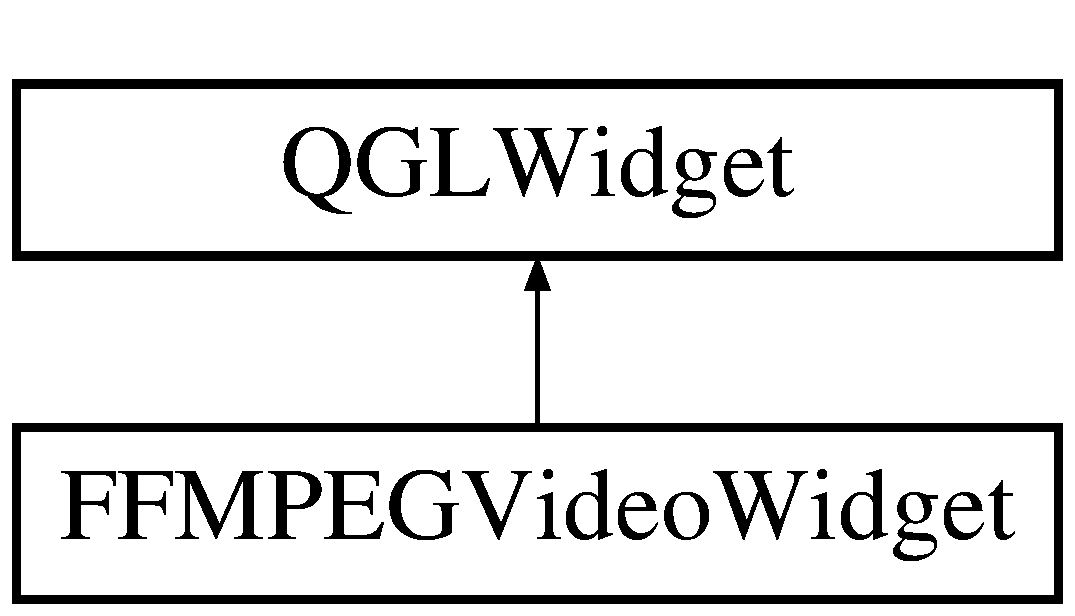
\includegraphics[height=2.000000cm]{classFFMPEGVideoWidget}
\end{center}
\end{figure}
\subsection*{Public Slots}
\begin{DoxyCompactItemize}
\item 
void \hyperlink{classFFMPEGVideoWidget_aa1c7cfdbf973cc553b4aca82f683df2a}{add\-Image} (Q\-Image $\ast$img)
\item 
void \hyperlink{classFFMPEGVideoWidget_a25da9d4dcf34bfabffd09f968d1bf6fb}{timer\-Tick} ()
\end{DoxyCompactItemize}
\subsection*{Signals}
\begin{DoxyCompactItemize}
\item 
void \hyperlink{classFFMPEGVideoWidget_a05576df29f811639d71cbed8b69ee233}{resize\-Parent} (int, int)
\end{DoxyCompactItemize}
\subsection*{Public Member Functions}
\begin{DoxyCompactItemize}
\item 
\hyperlink{classFFMPEGVideoWidget_af50a9f43743bfd96959a4ed57c7dd9c9}{F\-F\-M\-P\-E\-G\-Video\-Widget} (Q\-Widget $\ast$parent=0)
\item 
\hyperlink{classFFMPEGVideoWidget_a5c083d5fdadead8ecae1e8c024e8bdb4}{$\sim$\-F\-F\-M\-P\-E\-G\-Video\-Widget} ()
\item 
void \hyperlink{classFFMPEGVideoWidget_aa43fafb327e17f47b2a7b8cd55063ef3}{play} ()
\end{DoxyCompactItemize}
\subsection*{Protected Member Functions}
\begin{DoxyCompactItemize}
\item 
void \hyperlink{classFFMPEGVideoWidget_a4c0441e874e0186eca02d0ad750e4ca0}{paint\-Event} (Q\-Paint\-Event $\ast$e)
\end{DoxyCompactItemize}


\subsection{Constructor \& Destructor Documentation}
\hypertarget{classFFMPEGVideoWidget_af50a9f43743bfd96959a4ed57c7dd9c9}{\index{F\-F\-M\-P\-E\-G\-Video\-Widget@{F\-F\-M\-P\-E\-G\-Video\-Widget}!F\-F\-M\-P\-E\-G\-Video\-Widget@{F\-F\-M\-P\-E\-G\-Video\-Widget}}
\index{F\-F\-M\-P\-E\-G\-Video\-Widget@{F\-F\-M\-P\-E\-G\-Video\-Widget}!FFMPEGVideoWidget@{F\-F\-M\-P\-E\-G\-Video\-Widget}}
\subsubsection[{F\-F\-M\-P\-E\-G\-Video\-Widget}]{\setlength{\rightskip}{0pt plus 5cm}F\-F\-M\-P\-E\-G\-Video\-Widget\-::\-F\-F\-M\-P\-E\-G\-Video\-Widget (
\begin{DoxyParamCaption}
\item[{Q\-Widget $\ast$}]{parent = {\ttfamily 0}}
\end{DoxyParamCaption}
)\hspace{0.3cm}{\ttfamily [explicit]}}}\label{classFFMPEGVideoWidget_af50a9f43743bfd96959a4ed57c7dd9c9}

\begin{DoxyCode}
6                                                     :
7     QGLWidget(QGLFormat(QGL::SampleBuffers), parent),
8     first\_frame(\textcolor{keyword}{true})
9 \{
10     setFixedSize(320, 240);
11     setAutoFillBackground(\textcolor{keyword}{false});
12     \textcolor{comment}{//Set up the demuxer}
13     m\_demuxer = \textcolor{keyword}{new} \hyperlink{classDemuxer}{Demuxer}(QString(\hyperlink{ffmpegvideowidget_8h_aebde6daa4e9d1806e2c43f566475dfbe}{PIPENAME}));
14     m\_ffmpeg = \textcolor{keyword}{new} \hyperlink{classFFMPEGWrapper}{FFMPEGWrapper}(39082, m\_demuxer);
15     m\_ffmpeg\_thread = \textcolor{keyword}{new} QThread(\textcolor{keyword}{this});
16     m\_ffmpeg->moveToThread(m\_ffmpeg\_thread);
17     connect(m\_ffmpeg\_thread, SIGNAL(started()), m\_ffmpeg, SLOT(demux()));
18     connect(m\_ffmpeg, SIGNAL(finished()), m\_ffmpeg\_thread, SLOT(quit()));
19 
20     connect(m\_demuxer, SIGNAL(newImage(QImage *)), \textcolor{keyword}{this}, SLOT(\hyperlink{classFFMPEGVideoWidget_aa1c7cfdbf973cc553b4aca82f683df2a}{addImage}(QImage *)));
21 
22     \textcolor{comment}{//Set up the timer}
23     m\_timer = \textcolor{keyword}{new} QTimer(\textcolor{keyword}{this});
24     connect(m\_timer, SIGNAL(timeout()), \textcolor{keyword}{this}, SLOT(\hyperlink{classFFMPEGVideoWidget_a25da9d4dcf34bfabffd09f968d1bf6fb}{timerTick}()));
25 
26 \}
\end{DoxyCode}
\hypertarget{classFFMPEGVideoWidget_a5c083d5fdadead8ecae1e8c024e8bdb4}{\index{F\-F\-M\-P\-E\-G\-Video\-Widget@{F\-F\-M\-P\-E\-G\-Video\-Widget}!$\sim$\-F\-F\-M\-P\-E\-G\-Video\-Widget@{$\sim$\-F\-F\-M\-P\-E\-G\-Video\-Widget}}
\index{$\sim$\-F\-F\-M\-P\-E\-G\-Video\-Widget@{$\sim$\-F\-F\-M\-P\-E\-G\-Video\-Widget}!FFMPEGVideoWidget@{F\-F\-M\-P\-E\-G\-Video\-Widget}}
\subsubsection[{$\sim$\-F\-F\-M\-P\-E\-G\-Video\-Widget}]{\setlength{\rightskip}{0pt plus 5cm}F\-F\-M\-P\-E\-G\-Video\-Widget\-::$\sim$\-F\-F\-M\-P\-E\-G\-Video\-Widget (
\begin{DoxyParamCaption}
{}
\end{DoxyParamCaption}
)}}\label{classFFMPEGVideoWidget_a5c083d5fdadead8ecae1e8c024e8bdb4}

\begin{DoxyCode}
35 \{
36 \}
\end{DoxyCode}


\subsection{Member Function Documentation}
\hypertarget{classFFMPEGVideoWidget_aa1c7cfdbf973cc553b4aca82f683df2a}{\index{F\-F\-M\-P\-E\-G\-Video\-Widget@{F\-F\-M\-P\-E\-G\-Video\-Widget}!add\-Image@{add\-Image}}
\index{add\-Image@{add\-Image}!FFMPEGVideoWidget@{F\-F\-M\-P\-E\-G\-Video\-Widget}}
\subsubsection[{add\-Image}]{\setlength{\rightskip}{0pt plus 5cm}void F\-F\-M\-P\-E\-G\-Video\-Widget\-::add\-Image (
\begin{DoxyParamCaption}
\item[{Q\-Image $\ast$}]{img}
\end{DoxyParamCaption}
)\hspace{0.3cm}{\ttfamily [slot]}}}\label{classFFMPEGVideoWidget_aa1c7cfdbf973cc553b4aca82f683df2a}

\begin{DoxyCode}
39 \{
40     m\_buffer.push(img);
41 \}
\end{DoxyCode}
\hypertarget{classFFMPEGVideoWidget_a4c0441e874e0186eca02d0ad750e4ca0}{\index{F\-F\-M\-P\-E\-G\-Video\-Widget@{F\-F\-M\-P\-E\-G\-Video\-Widget}!paint\-Event@{paint\-Event}}
\index{paint\-Event@{paint\-Event}!FFMPEGVideoWidget@{F\-F\-M\-P\-E\-G\-Video\-Widget}}
\subsubsection[{paint\-Event}]{\setlength{\rightskip}{0pt plus 5cm}void F\-F\-M\-P\-E\-G\-Video\-Widget\-::paint\-Event (
\begin{DoxyParamCaption}
\item[{Q\-Paint\-Event $\ast$}]{e}
\end{DoxyParamCaption}
)\hspace{0.3cm}{\ttfamily [protected]}}}\label{classFFMPEGVideoWidget_a4c0441e874e0186eca02d0ad750e4ca0}

\begin{DoxyCode}
44 \{
45     \textcolor{keywordflow}{if}(!first\_frame)
46     \{
47 
48         QPainter p(\textcolor{keyword}{this});
49 
50         \textcolor{comment}{//Set the painter to use a smooth scaling algorithm.}
51        p.setRenderHint(QPainter::SmoothPixmapTransform);
52 
53         p.begin(\textcolor{keyword}{this});
54         p.drawImage(e->rect(), *current\_frame);
55         p.end();
56 
57 
58     \}
59 \}
\end{DoxyCode}
\hypertarget{classFFMPEGVideoWidget_aa43fafb327e17f47b2a7b8cd55063ef3}{\index{F\-F\-M\-P\-E\-G\-Video\-Widget@{F\-F\-M\-P\-E\-G\-Video\-Widget}!play@{play}}
\index{play@{play}!FFMPEGVideoWidget@{F\-F\-M\-P\-E\-G\-Video\-Widget}}
\subsubsection[{play}]{\setlength{\rightskip}{0pt plus 5cm}void F\-F\-M\-P\-E\-G\-Video\-Widget\-::play (
\begin{DoxyParamCaption}
{}
\end{DoxyParamCaption}
)}}\label{classFFMPEGVideoWidget_aa43fafb327e17f47b2a7b8cd55063ef3}

\begin{DoxyCode}
29 \{
30     m\_ffmpeg\_thread->start();
31     m\_timer->start(1000/30);
32 \}
\end{DoxyCode}
\hypertarget{classFFMPEGVideoWidget_a05576df29f811639d71cbed8b69ee233}{\index{F\-F\-M\-P\-E\-G\-Video\-Widget@{F\-F\-M\-P\-E\-G\-Video\-Widget}!resize\-Parent@{resize\-Parent}}
\index{resize\-Parent@{resize\-Parent}!FFMPEGVideoWidget@{F\-F\-M\-P\-E\-G\-Video\-Widget}}
\subsubsection[{resize\-Parent}]{\setlength{\rightskip}{0pt plus 5cm}void F\-F\-M\-P\-E\-G\-Video\-Widget\-::resize\-Parent (
\begin{DoxyParamCaption}
\item[{int}]{, }
\item[{int}]{}
\end{DoxyParamCaption}
)\hspace{0.3cm}{\ttfamily [signal]}}}\label{classFFMPEGVideoWidget_a05576df29f811639d71cbed8b69ee233}
\hypertarget{classFFMPEGVideoWidget_a25da9d4dcf34bfabffd09f968d1bf6fb}{\index{F\-F\-M\-P\-E\-G\-Video\-Widget@{F\-F\-M\-P\-E\-G\-Video\-Widget}!timer\-Tick@{timer\-Tick}}
\index{timer\-Tick@{timer\-Tick}!FFMPEGVideoWidget@{F\-F\-M\-P\-E\-G\-Video\-Widget}}
\subsubsection[{timer\-Tick}]{\setlength{\rightskip}{0pt plus 5cm}void F\-F\-M\-P\-E\-G\-Video\-Widget\-::timer\-Tick (
\begin{DoxyParamCaption}
{}
\end{DoxyParamCaption}
)\hspace{0.3cm}{\ttfamily [slot]}}}\label{classFFMPEGVideoWidget_a25da9d4dcf34bfabffd09f968d1bf6fb}

\begin{DoxyCode}
64 \{
65 
66     \textcolor{comment}{//Delete first frame}
67     \textcolor{keywordflow}{if}(!first\_frame)
68     \{
69         \textcolor{keywordflow}{if}(!m\_buffer.empty()) ;
70             \textcolor{keyword}{delete} current\_frame;
71     \}
72 
73     \textcolor{comment}{//Get the next frame}
74 
75     \textcolor{keywordflow}{if}(!m\_buffer.empty())
76     \{
77         \textcolor{keywordflow}{if}(first\_frame)
78             first\_frame = \textcolor{keyword}{false};
79         current\_frame = m\_buffer.front();
80         m\_buffer.pop();
81 
82         repaint();
83     \}
84 \}
\end{DoxyCode}


The documentation for this class was generated from the following files\-:\begin{DoxyCompactItemize}
\item 
U\-I/\hyperlink{ffmpegvideowidget_8h}{ffmpegvideowidget.\-h}\item 
U\-I/\hyperlink{ffmpegvideowidget_8cpp}{ffmpegvideowidget.\-cpp}\end{DoxyCompactItemize}

\hypertarget{classFFMPEGWrapper}{\section{F\-F\-M\-P\-E\-G\-Wrapper Class Reference}
\label{classFFMPEGWrapper}\index{F\-F\-M\-P\-E\-G\-Wrapper@{F\-F\-M\-P\-E\-G\-Wrapper}}
}


{\ttfamily \#include $<$ffmpegwrapper.\-h$>$}

Inheritance diagram for F\-F\-M\-P\-E\-G\-Wrapper\-:\begin{figure}[H]
\begin{center}
\leavevmode
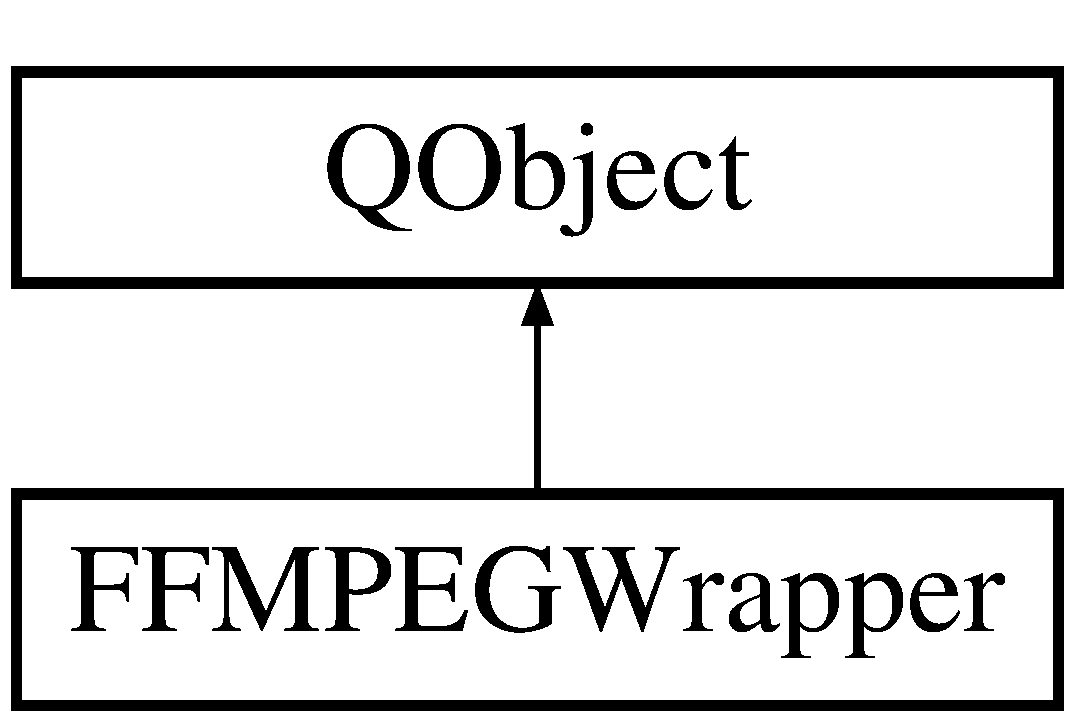
\includegraphics[height=2.000000cm]{classFFMPEGWrapper}
\end{center}
\end{figure}
\subsection*{Public Slots}
\begin{DoxyCompactItemize}
\item 
void \hyperlink{classFFMPEGWrapper_a29bfb04c36db41f6a5dfee2c2669fb81}{demux} ()
\item 
void \hyperlink{classFFMPEGWrapper_a649288e95daaf556db954729d479589d}{got\-Image} (Q\-Shared\-Pointer$<$ Q\-Image $>$ img)
\end{DoxyCompactItemize}
\subsection*{Signals}
\begin{DoxyCompactItemize}
\item 
void \hyperlink{classFFMPEGWrapper_a40ad147b791bb875802826466ea94cf9}{finished} ()
\item 
void \hyperlink{classFFMPEGWrapper_a91a7fbecacc6d1b82661accd2126f846}{new\-Image} (Q\-Shared\-Pointer$<$ Q\-Image $>$)
\end{DoxyCompactItemize}
\subsection*{Public Member Functions}
\begin{DoxyCompactItemize}
\item 
\hyperlink{classFFMPEGWrapper_a5dece5b4d3637569611eaa1bc0a4bfcf}{F\-F\-M\-P\-E\-G\-Wrapper} (int port, \hyperlink{classDemuxer}{Demuxer} $\ast$demuxer=N\-U\-L\-L, Q\-Object $\ast$parent=0)
\item 
bool \hyperlink{classFFMPEGWrapper_a15893a6ead5df825bfd25fd7a04eb18d}{is\-Demuxing} () const 
\item 
void \hyperlink{classFFMPEGWrapper_a8bf46fe65fdb28b5e5642cc84a4a2b57}{stop} ()
\end{DoxyCompactItemize}


\subsection{Constructor \& Destructor Documentation}
\hypertarget{classFFMPEGWrapper_a5dece5b4d3637569611eaa1bc0a4bfcf}{\index{F\-F\-M\-P\-E\-G\-Wrapper@{F\-F\-M\-P\-E\-G\-Wrapper}!F\-F\-M\-P\-E\-G\-Wrapper@{F\-F\-M\-P\-E\-G\-Wrapper}}
\index{F\-F\-M\-P\-E\-G\-Wrapper@{F\-F\-M\-P\-E\-G\-Wrapper}!FFMPEGWrapper@{F\-F\-M\-P\-E\-G\-Wrapper}}
\subsubsection[{F\-F\-M\-P\-E\-G\-Wrapper}]{\setlength{\rightskip}{0pt plus 5cm}F\-F\-M\-P\-E\-G\-Wrapper\-::\-F\-F\-M\-P\-E\-G\-Wrapper (
\begin{DoxyParamCaption}
\item[{int}]{port, }
\item[{{\bf Demuxer} $\ast$}]{demuxer = {\ttfamily NULL}, }
\item[{Q\-Object $\ast$}]{parent = {\ttfamily 0}}
\end{DoxyParamCaption}
)}}\label{classFFMPEGWrapper_a5dece5b4d3637569611eaa1bc0a4bfcf}

\begin{DoxyCode}
16                                                                         :
17     QObject(parent),
18     port(port)
19 \{
20     \textcolor{keywordflow}{if}(demuxer == NULL)
21         m\_demuxer = \textcolor{keyword}{new} \hyperlink{classDemuxer}{Demuxer}(QString(\hyperlink{ffmpegvideowidget_8h_aebde6daa4e9d1806e2c43f566475dfbe}{PIPENAME}));
22     \textcolor{keywordflow}{else}
23         m\_demuxer = demuxer;
24 
25     \textcolor{comment}{//Set up the demuxer thread}
26     m\_demux\_thread = \textcolor{keyword}{new} QThread(\textcolor{keyword}{this});
27     m\_demuxer->moveToThread(m\_demux\_thread);
28     connect(m\_demux\_thread, SIGNAL(started()), m\_demuxer, SLOT(\hyperlink{classFFMPEGWrapper_a29bfb04c36db41f6a5dfee2c2669fb81}{demux}()));
29     connect(m\_demuxer, SIGNAL(\hyperlink{classFFMPEGWrapper_a40ad147b791bb875802826466ea94cf9}{finished}()), m\_demux\_thread, SLOT(quit()));
30 
31 \}
\end{DoxyCode}


\subsection{Member Function Documentation}
\hypertarget{classFFMPEGWrapper_a29bfb04c36db41f6a5dfee2c2669fb81}{\index{F\-F\-M\-P\-E\-G\-Wrapper@{F\-F\-M\-P\-E\-G\-Wrapper}!demux@{demux}}
\index{demux@{demux}!FFMPEGWrapper@{F\-F\-M\-P\-E\-G\-Wrapper}}
\subsubsection[{demux}]{\setlength{\rightskip}{0pt plus 5cm}void F\-F\-M\-P\-E\-G\-Wrapper\-::demux (
\begin{DoxyParamCaption}
{}
\end{DoxyParamCaption}
)\hspace{0.3cm}{\ttfamily [slot]}}}\label{classFFMPEGWrapper_a29bfb04c36db41f6a5dfee2c2669fb81}

\begin{DoxyCode}
34 \{
35     \textcolor{keywordtype}{int} serv\_sockfd, num\_bytes;
36 
37     \textcolor{keywordtype}{char} packet[\hyperlink{ffmpegwrapper_8h_a0fa354abb723f3d7b1cdfea68545bb45}{PKT\_SIZE}];
38 
39     \textcolor{comment}{//The file}
40     FILE *buffer;
41 
42     \textcolor{comment}{//Storage for sender's address}
43     \textcolor{keyword}{struct }sockaddr\_storage their\_addr;
44     socklen\_t addr\_len;
45 
46     \textcolor{comment}{//Start a UDP server -- open up a port}
47     \textcolor{comment}{//Open a socket}
48     serv\_sockfd = socket(AF\_INET, SOCK\_DGRAM, IPPROTO\_UDP);
49     \textcolor{keywordflow}{if}(serv\_sockfd <= 0)
50     \{
51         \hyperlink{Log_8h_a1a242c34c5066fb0c62d909f22d3716d}{L\_ERROR}() << \textcolor{stringliteral}{"Failed to open socket."};
52         \textcolor{comment}{//perror("socket");}
53         \textcolor{keywordflow}{return};
54     \}
55 
56     \textcolor{comment}{//Bind to port on host side}
57     \textcolor{keyword}{struct }sockaddr\_in address;
58 
59     address.sin\_family = AF\_INET;
60     address.sin\_addr.s\_addr = INADDR\_ANY;
61     address.sin\_port = htons((\textcolor{keywordtype}{unsigned} \textcolor{keywordtype}{short}) port);
62 
63     \textcolor{keywordtype}{int} bound = bind(serv\_sockfd, (\textcolor{keyword}{struct} sockaddr *) &address, \textcolor{keyword}{sizeof}(address));
64     \textcolor{keywordflow}{if}(bound < 0)
65     \{
66         \hyperlink{Log_8h_a1a242c34c5066fb0c62d909f22d3716d}{L\_ERROR}() << \textcolor{stringliteral}{"Failed to bind socket to port"};
67         \textcolor{comment}{//perror("bind");}
68         \textcolor{keywordflow}{return};
69     \}
70 
71     \textcolor{comment}{//Create a named pipe (FIFO)}
72 
73     \textcolor{keywordtype}{char} *fifo = \hyperlink{ffmpegvideowidget_8h_aebde6daa4e9d1806e2c43f566475dfbe}{PIPENAME};
74     mkfifo(fifo, S\_IRUSR | S\_IWUSR | S\_IRGRP | S\_IWGRP | S\_IROTH);
75 
76     \textcolor{comment}{//=====CHANGE CODE HERE TO START A QT THREAD FOR DEMUXER OBJ TO PERFORM ITS WORK}
77     m\_demux\_thread->start();
78 
79     \textcolor{comment}{//Open pipe}
80     \textcolor{comment}{//Open the file}
81     \textcolor{keywordflow}{if}((buffer = fopen(\hyperlink{ffmpegvideowidget_8h_aebde6daa4e9d1806e2c43f566475dfbe}{PIPENAME}, \textcolor{stringliteral}{"wb"})) == NULL)
82     \{
83         \textcolor{comment}{//perror("fopen");}
84         \textcolor{comment}{//exit(1);}
85     \}
86 
87     is\_demuxing = \textcolor{keyword}{true};
88 
89     \hyperlink{Log_8h_a7cec51f4ce4b22e8c0f256485d57fca7}{INFO}() << \textcolor{stringliteral}{"Start demuxing"};
90 
91     \textcolor{keywordflow}{while}(is\_demuxing)
92     \{
93 
94         memset(packet, 0, \hyperlink{ffmpegwrapper_8h_a0fa354abb723f3d7b1cdfea68545bb45}{PKT\_SIZE});
95 
96         \textcolor{comment}{//Get next packet}
97         \textcolor{keywordflow}{if}((num\_bytes = recvfrom(serv\_sockfd, packet, \hyperlink{ffmpegwrapper_8h_a0fa354abb723f3d7b1cdfea68545bb45}{PKT\_SIZE}, 0,
98             (\textcolor{keyword}{struct} sockaddr *)&their\_addr, &addr\_len)) == -1)
99         \{
100             \textcolor{keywordflow}{if}(errno != EAGAIN)
101             \{
102                 \hyperlink{Log_8h_a1a242c34c5066fb0c62d909f22d3716d}{L\_ERROR}() << \textcolor{stringliteral}{"recvfrom: "} << strerror(errno);
103                 is\_demuxing = \textcolor{keyword}{false};
104             \}
105         \}
106 
107         \textcolor{keywordflow}{if}(errno != EAGAIN)
108         \{
109             \textcolor{keywordtype}{char} *dat = packet;
110             \textcolor{comment}{//if(packet[4] != 0x67 && packet[4] != 0x65)}
111             \textcolor{comment}{//\{}
112                 \textcolor{comment}{//dat++;}
113                 \textcolor{comment}{//num\_bytes--;}
114             \textcolor{comment}{//\}}
115             \textcolor{comment}{//Write to file}
116             fwrite(dat, \textcolor{keyword}{sizeof}(\textcolor{keywordtype}{char}), (num\_bytes) / \textcolor{keyword}{sizeof}(\textcolor{keywordtype}{char}), buffer);
117         \}
118 
119     \}
120 
121     \hyperlink{Log_8h_a7cec51f4ce4b22e8c0f256485d57fca7}{INFO}() << \textcolor{stringliteral}{"End demuxing"};
122     close(serv\_sockfd);
123     fclose(buffer);
124 
125     emit \hyperlink{classFFMPEGWrapper_a40ad147b791bb875802826466ea94cf9}{finished}();
126 
127     \textcolor{keywordflow}{return};
128 
129 \}
\end{DoxyCode}
\hypertarget{classFFMPEGWrapper_a40ad147b791bb875802826466ea94cf9}{\index{F\-F\-M\-P\-E\-G\-Wrapper@{F\-F\-M\-P\-E\-G\-Wrapper}!finished@{finished}}
\index{finished@{finished}!FFMPEGWrapper@{F\-F\-M\-P\-E\-G\-Wrapper}}
\subsubsection[{finished}]{\setlength{\rightskip}{0pt plus 5cm}void F\-F\-M\-P\-E\-G\-Wrapper\-::finished (
\begin{DoxyParamCaption}
{}
\end{DoxyParamCaption}
)\hspace{0.3cm}{\ttfamily [signal]}}}\label{classFFMPEGWrapper_a40ad147b791bb875802826466ea94cf9}
\hypertarget{classFFMPEGWrapper_a649288e95daaf556db954729d479589d}{\index{F\-F\-M\-P\-E\-G\-Wrapper@{F\-F\-M\-P\-E\-G\-Wrapper}!got\-Image@{got\-Image}}
\index{got\-Image@{got\-Image}!FFMPEGWrapper@{F\-F\-M\-P\-E\-G\-Wrapper}}
\subsubsection[{got\-Image}]{\setlength{\rightskip}{0pt plus 5cm}void F\-F\-M\-P\-E\-G\-Wrapper\-::got\-Image (
\begin{DoxyParamCaption}
\item[{Q\-Shared\-Pointer$<$ Q\-Image $>$}]{img}
\end{DoxyParamCaption}
)\hspace{0.3cm}{\ttfamily [slot]}}}\label{classFFMPEGWrapper_a649288e95daaf556db954729d479589d}

\begin{DoxyCode}
132 \{
133     emit \hyperlink{classFFMPEGWrapper_a91a7fbecacc6d1b82661accd2126f846}{newImage}(img);
134 \}
\end{DoxyCode}
\hypertarget{classFFMPEGWrapper_a15893a6ead5df825bfd25fd7a04eb18d}{\index{F\-F\-M\-P\-E\-G\-Wrapper@{F\-F\-M\-P\-E\-G\-Wrapper}!is\-Demuxing@{is\-Demuxing}}
\index{is\-Demuxing@{is\-Demuxing}!FFMPEGWrapper@{F\-F\-M\-P\-E\-G\-Wrapper}}
\subsubsection[{is\-Demuxing}]{\setlength{\rightskip}{0pt plus 5cm}bool F\-F\-M\-P\-E\-G\-Wrapper\-::is\-Demuxing (
\begin{DoxyParamCaption}
{}
\end{DoxyParamCaption}
) const}}\label{classFFMPEGWrapper_a15893a6ead5df825bfd25fd7a04eb18d}

\begin{DoxyCode}
138 \{
139     \textcolor{keywordflow}{return} is\_demuxing;
140 \}
\end{DoxyCode}
\hypertarget{classFFMPEGWrapper_a91a7fbecacc6d1b82661accd2126f846}{\index{F\-F\-M\-P\-E\-G\-Wrapper@{F\-F\-M\-P\-E\-G\-Wrapper}!new\-Image@{new\-Image}}
\index{new\-Image@{new\-Image}!FFMPEGWrapper@{F\-F\-M\-P\-E\-G\-Wrapper}}
\subsubsection[{new\-Image}]{\setlength{\rightskip}{0pt plus 5cm}void F\-F\-M\-P\-E\-G\-Wrapper\-::new\-Image (
\begin{DoxyParamCaption}
\item[{Q\-Shared\-Pointer$<$ Q\-Image $>$}]{}
\end{DoxyParamCaption}
)\hspace{0.3cm}{\ttfamily [signal]}}}\label{classFFMPEGWrapper_a91a7fbecacc6d1b82661accd2126f846}
\hypertarget{classFFMPEGWrapper_a8bf46fe65fdb28b5e5642cc84a4a2b57}{\index{F\-F\-M\-P\-E\-G\-Wrapper@{F\-F\-M\-P\-E\-G\-Wrapper}!stop@{stop}}
\index{stop@{stop}!FFMPEGWrapper@{F\-F\-M\-P\-E\-G\-Wrapper}}
\subsubsection[{stop}]{\setlength{\rightskip}{0pt plus 5cm}void F\-F\-M\-P\-E\-G\-Wrapper\-::stop (
\begin{DoxyParamCaption}
{}
\end{DoxyParamCaption}
)}}\label{classFFMPEGWrapper_a8bf46fe65fdb28b5e5642cc84a4a2b57}

\begin{DoxyCode}
143 \{
144     is\_demuxing = \textcolor{keyword}{false};
145 \}
\end{DoxyCode}


The documentation for this class was generated from the following files\-:\begin{DoxyCompactItemize}
\item 
Video/\hyperlink{ffmpegwrapper_8h}{ffmpegwrapper.\-h}\item 
Video/\hyperlink{ffmpegwrapper_8cpp}{ffmpegwrapper.\-cpp}\end{DoxyCompactItemize}

\hypertarget{classFileReaderUtility}{\section{File\-Reader\-Utility Class Reference}
\label{classFileReaderUtility}\index{File\-Reader\-Utility@{File\-Reader\-Utility}}
}


A class to parse a file, specifically to generate a list of strings which are the lines of that file.  




{\ttfamily \#include $<$filereaderutility.\-h$>$}

\subsection*{Public Member Functions}
\begin{DoxyCompactItemize}
\item 
\hyperlink{classFileReaderUtility_a6cabb02a585207c222063e17c23bc345}{File\-Reader\-Utility} ()
\begin{DoxyCompactList}\small\item\em Default value contructor. \end{DoxyCompactList}\item 
\hyperlink{classFileReaderUtility_a470ee17457de07fe519aaf8e607a82bc}{File\-Reader\-Utility} (Q\-String filename)
\begin{DoxyCompactList}\small\item\em Explicit value constructor. \end{DoxyCompactList}\item 
\hyperlink{classFileReaderUtility_ae7cea9f17577620d7c678d8379ee103c}{$\sim$\-File\-Reader\-Utility} ()
\item 
void \hyperlink{classFileReaderUtility_a8d4984a9b7f18c589906d6e26956402b}{set\-File} (const Q\-String \&filename)
\begin{DoxyCompactList}\small\item\em set\-File Sets the current filename to open in the \hyperlink{classFileReaderUtility_a77c879620e0ddcc16e966649a73aa5c5}{open\-\_\-file()} call \end{DoxyCompactList}\item 
Q\-String \hyperlink{classFileReaderUtility_a9a871c01eeb7336d5d2cbc90d1550d3d}{get\-File} () const 
\begin{DoxyCompactList}\small\item\em Get the file path. \end{DoxyCompactList}\item 
bool \hyperlink{classFileReaderUtility_a77c879620e0ddcc16e966649a73aa5c5}{open\-\_\-file} ()
\begin{DoxyCompactList}\small\item\em Open the file. \end{DoxyCompactList}\item 
void \hyperlink{classFileReaderUtility_ab8c0f909bc4d5325ad062a35451442a5}{close} ()
\begin{DoxyCompactList}\small\item\em Close the file. \end{DoxyCompactList}\item 
bool \hyperlink{classFileReaderUtility_a0e8f0a86678ed4690758abad92d08520}{is\-Open} ()
\begin{DoxyCompactList}\small\item\em is\-Open Whether or not a file is open. \end{DoxyCompactList}\item 
Q\-String\-List \& \hyperlink{classFileReaderUtility_af0efa92dc11188682345ba1d587993a7}{parse} ()
\begin{DoxyCompactList}\small\item\em parse This function will parse the opened file and return a list of strings (each line in the file) \end{DoxyCompactList}\item 
Q\-String \hyperlink{classFileReaderUtility_ab41fc317ab5f175f61a15f1c2dff20ab}{read\-Line} ()
\begin{DoxyCompactList}\small\item\em Read one line of the file. \end{DoxyCompactList}\end{DoxyCompactItemize}


\subsection{Detailed Description}
A class to parse a file, specifically to generate a list of strings which are the lines of that file. 

\subsection{Constructor \& Destructor Documentation}
\hypertarget{classFileReaderUtility_a6cabb02a585207c222063e17c23bc345}{\index{File\-Reader\-Utility@{File\-Reader\-Utility}!File\-Reader\-Utility@{File\-Reader\-Utility}}
\index{File\-Reader\-Utility@{File\-Reader\-Utility}!FileReaderUtility@{File\-Reader\-Utility}}
\subsubsection[{File\-Reader\-Utility}]{\setlength{\rightskip}{0pt plus 5cm}File\-Reader\-Utility\-::\-File\-Reader\-Utility (
\begin{DoxyParamCaption}
{}
\end{DoxyParamCaption}
)}}\label{classFileReaderUtility_a6cabb02a585207c222063e17c23bc345}


Default value contructor. 


\begin{DoxyCode}
4                                      :
5     m\_filename(\textcolor{stringliteral}{""}),
6     m\_isOpen(\textcolor{keyword}{false}),
7     m\_lines(QStringList()),
8     m\_infile(NULL),
9     m\_stream(NULL)
10 \{
11 
12 \}
\end{DoxyCode}
\hypertarget{classFileReaderUtility_a470ee17457de07fe519aaf8e607a82bc}{\index{File\-Reader\-Utility@{File\-Reader\-Utility}!File\-Reader\-Utility@{File\-Reader\-Utility}}
\index{File\-Reader\-Utility@{File\-Reader\-Utility}!FileReaderUtility@{File\-Reader\-Utility}}
\subsubsection[{File\-Reader\-Utility}]{\setlength{\rightskip}{0pt plus 5cm}File\-Reader\-Utility\-::\-File\-Reader\-Utility (
\begin{DoxyParamCaption}
\item[{Q\-String}]{filename}
\end{DoxyParamCaption}
)}}\label{classFileReaderUtility_a470ee17457de07fe519aaf8e607a82bc}


Explicit value constructor. 


\begin{DoxyParams}{Parameters}
{\em filename} & The file to read from. \\
\hline
\end{DoxyParams}

\begin{DoxyCode}
14                                                      :
15     m\_filename(filename),
16     m\_isOpen(\textcolor{keyword}{false}),
17     m\_lines(QStringList()),
18     m\_infile(NULL),
19     m\_stream(NULL)
20 \{
21 \}
\end{DoxyCode}
\hypertarget{classFileReaderUtility_ae7cea9f17577620d7c678d8379ee103c}{\index{File\-Reader\-Utility@{File\-Reader\-Utility}!$\sim$\-File\-Reader\-Utility@{$\sim$\-File\-Reader\-Utility}}
\index{$\sim$\-File\-Reader\-Utility@{$\sim$\-File\-Reader\-Utility}!FileReaderUtility@{File\-Reader\-Utility}}
\subsubsection[{$\sim$\-File\-Reader\-Utility}]{\setlength{\rightskip}{0pt plus 5cm}File\-Reader\-Utility\-::$\sim$\-File\-Reader\-Utility (
\begin{DoxyParamCaption}
{}
\end{DoxyParamCaption}
)}}\label{classFileReaderUtility_ae7cea9f17577620d7c678d8379ee103c}

\begin{DoxyCode}
24 \{
25     this->\hyperlink{classFileReaderUtility_ab8c0f909bc4d5325ad062a35451442a5}{close}();
26 \}
\end{DoxyCode}


\subsection{Member Function Documentation}
\hypertarget{classFileReaderUtility_ab8c0f909bc4d5325ad062a35451442a5}{\index{File\-Reader\-Utility@{File\-Reader\-Utility}!close@{close}}
\index{close@{close}!FileReaderUtility@{File\-Reader\-Utility}}
\subsubsection[{close}]{\setlength{\rightskip}{0pt plus 5cm}void File\-Reader\-Utility\-::close (
\begin{DoxyParamCaption}
{}
\end{DoxyParamCaption}
)}}\label{classFileReaderUtility_ab8c0f909bc4d5325ad062a35451442a5}


Close the file. 


\begin{DoxyCode}
57 \{
58     \textcolor{keywordflow}{if}(this->\hyperlink{classFileReaderUtility_a0e8f0a86678ed4690758abad92d08520}{isOpen}())
59     \{
60         m\_infile->close();
61         m\_isOpen = \textcolor{keyword}{false};
62 
63         \textcolor{comment}{//Delete resources}
64         \textcolor{keyword}{delete} m\_infile;
65         m\_infile = NULL;
66         \textcolor{keyword}{delete} m\_stream;
67         m\_stream = NULL;
68     \}
69 \}
\end{DoxyCode}
\hypertarget{classFileReaderUtility_a9a871c01eeb7336d5d2cbc90d1550d3d}{\index{File\-Reader\-Utility@{File\-Reader\-Utility}!get\-File@{get\-File}}
\index{get\-File@{get\-File}!FileReaderUtility@{File\-Reader\-Utility}}
\subsubsection[{get\-File}]{\setlength{\rightskip}{0pt plus 5cm}Q\-String File\-Reader\-Utility\-::get\-File (
\begin{DoxyParamCaption}
{}
\end{DoxyParamCaption}
) const}}\label{classFileReaderUtility_a9a871c01eeb7336d5d2cbc90d1550d3d}


Get the file path. 

\begin{DoxyReturn}{Returns}
The path to the file in use. 
\end{DoxyReturn}

\begin{DoxyCode}
34 \{
35     \textcolor{keywordflow}{return} this->m\_filename;
36 \}
\end{DoxyCode}
\hypertarget{classFileReaderUtility_a0e8f0a86678ed4690758abad92d08520}{\index{File\-Reader\-Utility@{File\-Reader\-Utility}!is\-Open@{is\-Open}}
\index{is\-Open@{is\-Open}!FileReaderUtility@{File\-Reader\-Utility}}
\subsubsection[{is\-Open}]{\setlength{\rightskip}{0pt plus 5cm}bool File\-Reader\-Utility\-::is\-Open (
\begin{DoxyParamCaption}
{}
\end{DoxyParamCaption}
)}}\label{classFileReaderUtility_a0e8f0a86678ed4690758abad92d08520}


is\-Open Whether or not a file is open. 

\begin{DoxyReturn}{Returns}
true if the file is open 
\end{DoxyReturn}

\begin{DoxyCode}
72 \{
73     \textcolor{keywordflow}{return} m\_isOpen;
74 \}
\end{DoxyCode}
\hypertarget{classFileReaderUtility_a77c879620e0ddcc16e966649a73aa5c5}{\index{File\-Reader\-Utility@{File\-Reader\-Utility}!open\-\_\-file@{open\-\_\-file}}
\index{open\-\_\-file@{open\-\_\-file}!FileReaderUtility@{File\-Reader\-Utility}}
\subsubsection[{open\-\_\-file}]{\setlength{\rightskip}{0pt plus 5cm}bool File\-Reader\-Utility\-::open\-\_\-file (
\begin{DoxyParamCaption}
{}
\end{DoxyParamCaption}
)}}\label{classFileReaderUtility_a77c879620e0ddcc16e966649a73aa5c5}


Open the file. 

This function will open the file specified by the m\-\_\-filename field. \begin{DoxyReturn}{Returns}
true if the file successfully opened, false otherwise. 
\end{DoxyReturn}

\begin{DoxyCode}
39 \{
40     \textcolor{comment}{//Open the file}
41     m\_infile = \textcolor{keyword}{new} QFile(m\_filename);
42     m\_isOpen = m\_infile->open(QIODevice::ReadOnly);
43 
44     \textcolor{keywordflow}{if}(m\_isOpen)
45     \{
46         \textcolor{comment}{//Open a text stream;}
47         m\_stream = \textcolor{keyword}{new} QTextStream(m\_infile);
48     \}
49 
50     \textcolor{comment}{//Open read only}
51     \textcolor{keywordflow}{return} m\_isOpen;
52 
53 \}
\end{DoxyCode}
\hypertarget{classFileReaderUtility_af0efa92dc11188682345ba1d587993a7}{\index{File\-Reader\-Utility@{File\-Reader\-Utility}!parse@{parse}}
\index{parse@{parse}!FileReaderUtility@{File\-Reader\-Utility}}
\subsubsection[{parse}]{\setlength{\rightskip}{0pt plus 5cm}Q\-String\-List \& File\-Reader\-Utility\-::parse (
\begin{DoxyParamCaption}
{}
\end{DoxyParamCaption}
)}}\label{classFileReaderUtility_af0efa92dc11188682345ba1d587993a7}


parse This function will parse the opened file and return a list of strings (each line in the file) 

\begin{DoxyReturn}{Returns}
A list of strings (each line in the file) 
\end{DoxyReturn}

\begin{DoxyCode}
77 \{
78     \textcolor{comment}{//See if the file is open}
79     \textcolor{keywordflow}{if}(!m\_isOpen)
80         \textcolor{keywordflow}{return} m\_lines;
81 
82     \textcolor{comment}{//Create an input stream}
83     QTextStream input\_stream(m\_infile);
84 
85     \textcolor{comment}{//Parse each line}
86     \textcolor{keywordflow}{while}(!input\_stream.atEnd())
87     \{
88         \textcolor{comment}{//Get next line}
89         QString next = input\_stream.readLine();
90         m\_lines << next;
91 
92     \}
93 
94     this->\hyperlink{classFileReaderUtility_ab8c0f909bc4d5325ad062a35451442a5}{close}();
95 
96     \textcolor{keywordflow}{return} m\_lines;
97 
98 \}
\end{DoxyCode}
\hypertarget{classFileReaderUtility_ab41fc317ab5f175f61a15f1c2dff20ab}{\index{File\-Reader\-Utility@{File\-Reader\-Utility}!read\-Line@{read\-Line}}
\index{read\-Line@{read\-Line}!FileReaderUtility@{File\-Reader\-Utility}}
\subsubsection[{read\-Line}]{\setlength{\rightskip}{0pt plus 5cm}Q\-String File\-Reader\-Utility\-::read\-Line (
\begin{DoxyParamCaption}
{}
\end{DoxyParamCaption}
)}}\label{classFileReaderUtility_ab41fc317ab5f175f61a15f1c2dff20ab}


Read one line of the file. 

\begin{DoxyReturn}{Returns}
The next line of the file to read. 
\end{DoxyReturn}

\begin{DoxyCode}
102 \{
103     QString next(\textcolor{stringliteral}{""});
104     \textcolor{comment}{//See if the file is open}
105     \textcolor{keywordflow}{if}(!m\_isOpen)
106         \textcolor{keywordflow}{return} next;
107 
108     \textcolor{comment}{//Create an input stream}
109     \textcolor{comment}{//QTextStream input\_stream(m\_infile);}
110 
111     \textcolor{keywordflow}{if}(this->\hyperlink{classFileReaderUtility_a0e8f0a86678ed4690758abad92d08520}{isOpen}())
112     \{
113         \textcolor{comment}{//Read the next line}
114         next = m\_stream->readLine();
115         m\_lines << next;
116 
117     \}
118     \textcolor{keywordflow}{else}
119         this->\hyperlink{classFileReaderUtility_ab8c0f909bc4d5325ad062a35451442a5}{close}();
120 
121     \textcolor{keywordflow}{return} next;
122 
123 \}
\end{DoxyCode}
\hypertarget{classFileReaderUtility_a8d4984a9b7f18c589906d6e26956402b}{\index{File\-Reader\-Utility@{File\-Reader\-Utility}!set\-File@{set\-File}}
\index{set\-File@{set\-File}!FileReaderUtility@{File\-Reader\-Utility}}
\subsubsection[{set\-File}]{\setlength{\rightskip}{0pt plus 5cm}void File\-Reader\-Utility\-::set\-File (
\begin{DoxyParamCaption}
\item[{const Q\-String \&}]{filename}
\end{DoxyParamCaption}
)}}\label{classFileReaderUtility_a8d4984a9b7f18c589906d6e26956402b}


set\-File Sets the current filename to open in the \hyperlink{classFileReaderUtility_a77c879620e0ddcc16e966649a73aa5c5}{open\-\_\-file()} call 


\begin{DoxyParams}{Parameters}
{\em filename} & The name of the file \\
\hline
\end{DoxyParams}

\begin{DoxyCode}
29 \{
30     m\_filename = filename;
31 \}
\end{DoxyCode}


The documentation for this class was generated from the following files\-:\begin{DoxyCompactItemize}
\item 
Util/\-File\-Util/\hyperlink{filereaderutility_8h}{filereaderutility.\-h}\item 
Util/\-File\-Util/\hyperlink{filereaderutility_8cpp}{filereaderutility.\-cpp}\end{DoxyCompactItemize}

\hypertarget{structgap}{\section{gap Struct Reference}
\label{structgap}\index{gap@{gap}}
}
\subsection*{Public Member Functions}
\begin{DoxyCompactItemize}
\item 
\hyperlink{structgap_a4ae36e370647da0df57eb30d3bbcd32b}{gap} ()
\item 
void \hyperlink{structgap_a9c0d0b12bc778c8439c8aec7747ab2b0}{push} (char\-\_\-t $\ast$\&s, size\-\_\-t count)
\item 
char\-\_\-t $\ast$ \hyperlink{structgap_a176c58ee8d57c41b91ae9f00d5e8cab5}{flush} (char\-\_\-t $\ast$s)
\end{DoxyCompactItemize}
\subsection*{Data Fields}
\begin{DoxyCompactItemize}
\item 
char\-\_\-t $\ast$ \hyperlink{structgap_a1fafd4d9909a3413f723f24e46dfde0e}{end}
\item 
size\-\_\-t \hyperlink{structgap_ad5bb3597ade78d89bbe0e300748ad508}{size}
\end{DoxyCompactItemize}


\subsection{Constructor \& Destructor Documentation}
\hypertarget{structgap_a4ae36e370647da0df57eb30d3bbcd32b}{\index{gap@{gap}!gap@{gap}}
\index{gap@{gap}!gap@{gap}}
\subsubsection[{gap}]{\setlength{\rightskip}{0pt plus 5cm}gap\-::gap (
\begin{DoxyParamCaption}
{}
\end{DoxyParamCaption}
)\hspace{0.3cm}{\ttfamily [inline]}}}\label{structgap_a4ae36e370647da0df57eb30d3bbcd32b}

\begin{DoxyCode}
1577              : \hyperlink{structgap_a1fafd4d9909a3413f723f24e46dfde0e}{end}(0), \hyperlink{structgap_ad5bb3597ade78d89bbe0e300748ad508}{size}(0)
1578         \{
1579         \}
\end{DoxyCode}


\subsection{Member Function Documentation}
\hypertarget{structgap_a176c58ee8d57c41b91ae9f00d5e8cab5}{\index{gap@{gap}!flush@{flush}}
\index{flush@{flush}!gap@{gap}}
\subsubsection[{flush}]{\setlength{\rightskip}{0pt plus 5cm}char\-\_\-t$\ast$ gap\-::flush (
\begin{DoxyParamCaption}
\item[{char\-\_\-t $\ast$}]{s}
\end{DoxyParamCaption}
)\hspace{0.3cm}{\ttfamily [inline]}}}\label{structgap_a176c58ee8d57c41b91ae9f00d5e8cab5}

\begin{DoxyCode}
1601         \{
1602             \textcolor{keywordflow}{if} (\hyperlink{structgap_a1fafd4d9909a3413f723f24e46dfde0e}{end})
1603             \{
1604                 \textcolor{comment}{// Move [old\_gap\_end, current\_pos) to [old\_gap\_start, ...)}
1605                 assert(s >= \hyperlink{structgap_a1fafd4d9909a3413f723f24e46dfde0e}{end});
1606                 memmove(\hyperlink{structgap_a1fafd4d9909a3413f723f24e46dfde0e}{end} - \hyperlink{structgap_ad5bb3597ade78d89bbe0e300748ad508}{size}, \hyperlink{structgap_a1fafd4d9909a3413f723f24e46dfde0e}{end}, reinterpret\_cast<char*>(s) - reinterpret\_cast<char*>(
      \hyperlink{structgap_a1fafd4d9909a3413f723f24e46dfde0e}{end}));
1607 
1608                 \textcolor{keywordflow}{return} s - \hyperlink{structgap_ad5bb3597ade78d89bbe0e300748ad508}{size};
1609             \}
1610             \textcolor{keywordflow}{else} \textcolor{keywordflow}{return} s;
1611         \}
\end{DoxyCode}
\hypertarget{structgap_a9c0d0b12bc778c8439c8aec7747ab2b0}{\index{gap@{gap}!push@{push}}
\index{push@{push}!gap@{gap}}
\subsubsection[{push}]{\setlength{\rightskip}{0pt plus 5cm}void gap\-::push (
\begin{DoxyParamCaption}
\item[{char\-\_\-t $\ast$\&}]{s, }
\item[{size\-\_\-t}]{count}
\end{DoxyParamCaption}
)\hspace{0.3cm}{\ttfamily [inline]}}}\label{structgap_a9c0d0b12bc778c8439c8aec7747ab2b0}

\begin{DoxyCode}
1584         \{
1585             \textcolor{keywordflow}{if} (\hyperlink{structgap_a1fafd4d9909a3413f723f24e46dfde0e}{end}) \textcolor{comment}{// there was a gap already; collapse it}
1586             \{
1587                 \textcolor{comment}{// Move [old\_gap\_end, new\_gap\_start) to [old\_gap\_start, ...)}
1588                 assert(s >= \hyperlink{structgap_a1fafd4d9909a3413f723f24e46dfde0e}{end});
1589                 memmove(\hyperlink{structgap_a1fafd4d9909a3413f723f24e46dfde0e}{end} - \hyperlink{structgap_ad5bb3597ade78d89bbe0e300748ad508}{size}, \hyperlink{structgap_a1fafd4d9909a3413f723f24e46dfde0e}{end}, reinterpret\_cast<char*>(s) - reinterpret\_cast<char*>(
      \hyperlink{structgap_a1fafd4d9909a3413f723f24e46dfde0e}{end}));
1590             \}
1591                 
1592             s += count; \textcolor{comment}{// end of current gap}
1593                 
1594             \textcolor{comment}{// "merge" two gaps}
1595             \hyperlink{structgap_a1fafd4d9909a3413f723f24e46dfde0e}{end} = s;
1596             \hyperlink{structgap_ad5bb3597ade78d89bbe0e300748ad508}{size} += count;
1597         \}
\end{DoxyCode}


\subsection{Field Documentation}
\hypertarget{structgap_a1fafd4d9909a3413f723f24e46dfde0e}{\index{gap@{gap}!end@{end}}
\index{end@{end}!gap@{gap}}
\subsubsection[{end}]{\setlength{\rightskip}{0pt plus 5cm}char\-\_\-t$\ast$ gap\-::end}}\label{structgap_a1fafd4d9909a3413f723f24e46dfde0e}
\hypertarget{structgap_ad5bb3597ade78d89bbe0e300748ad508}{\index{gap@{gap}!size@{size}}
\index{size@{size}!gap@{gap}}
\subsubsection[{size}]{\setlength{\rightskip}{0pt plus 5cm}size\-\_\-t gap\-::size}}\label{structgap_ad5bb3597ade78d89bbe0e300748ad508}


The documentation for this struct was generated from the following file\-:\begin{DoxyCompactItemize}
\item 
Third\-Party/pugixml/\hyperlink{pugixml_8cpp}{pugixml.\-cpp}\end{DoxyCompactItemize}

\hypertarget{structlatin1__writer}{\section{latin1\-\_\-writer Struct Reference}
\label{structlatin1__writer}\index{latin1\-\_\-writer@{latin1\-\_\-writer}}
}
\subsection*{Public Types}
\begin{DoxyCompactItemize}
\item 
typedef uint8\-\_\-t $\ast$ \hyperlink{structlatin1__writer_af9228600fa7eecd793cc3d927d46eb1a}{value\-\_\-type}
\end{DoxyCompactItemize}
\subsection*{Static Public Member Functions}
\begin{DoxyCompactItemize}
\item 
static \hyperlink{structlatin1__writer_af9228600fa7eecd793cc3d927d46eb1a}{value\-\_\-type} \hyperlink{structlatin1__writer_ab5d7a833d29d66031420686ca67b1f6e}{low} (\hyperlink{structlatin1__writer_af9228600fa7eecd793cc3d927d46eb1a}{value\-\_\-type} result, uint32\-\_\-t ch)
\item 
static \hyperlink{structlatin1__writer_af9228600fa7eecd793cc3d927d46eb1a}{value\-\_\-type} \hyperlink{structlatin1__writer_a0e48c306ebe556f267404a9624f00554}{high} (\hyperlink{structlatin1__writer_af9228600fa7eecd793cc3d927d46eb1a}{value\-\_\-type} result, uint32\-\_\-t ch)
\end{DoxyCompactItemize}


\subsection{Member Typedef Documentation}
\hypertarget{structlatin1__writer_af9228600fa7eecd793cc3d927d46eb1a}{\index{latin1\-\_\-writer@{latin1\-\_\-writer}!value\-\_\-type@{value\-\_\-type}}
\index{value\-\_\-type@{value\-\_\-type}!latin1_writer@{latin1\-\_\-writer}}
\subsubsection[{value\-\_\-type}]{\setlength{\rightskip}{0pt plus 5cm}typedef uint8\-\_\-t$\ast$ {\bf latin1\-\_\-writer\-::value\-\_\-type}}}\label{structlatin1__writer_af9228600fa7eecd793cc3d927d46eb1a}


\subsection{Member Function Documentation}
\hypertarget{structlatin1__writer_a0e48c306ebe556f267404a9624f00554}{\index{latin1\-\_\-writer@{latin1\-\_\-writer}!high@{high}}
\index{high@{high}!latin1_writer@{latin1\-\_\-writer}}
\subsubsection[{high}]{\setlength{\rightskip}{0pt plus 5cm}static {\bf value\-\_\-type} latin1\-\_\-writer\-::high (
\begin{DoxyParamCaption}
\item[{{\bf value\-\_\-type}}]{result, }
\item[{uint32\-\_\-t}]{ch}
\end{DoxyParamCaption}
)\hspace{0.3cm}{\ttfamily [inline]}, {\ttfamily [static]}}}\label{structlatin1__writer_a0e48c306ebe556f267404a9624f00554}

\begin{DoxyCode}
817         \{
818             (void)ch;
819 
820             *result = \textcolor{charliteral}{'?'};
821 
822             \textcolor{keywordflow}{return} result + 1;
823         \}
\end{DoxyCode}
\hypertarget{structlatin1__writer_ab5d7a833d29d66031420686ca67b1f6e}{\index{latin1\-\_\-writer@{latin1\-\_\-writer}!low@{low}}
\index{low@{low}!latin1_writer@{latin1\-\_\-writer}}
\subsubsection[{low}]{\setlength{\rightskip}{0pt plus 5cm}static {\bf value\-\_\-type} latin1\-\_\-writer\-::low (
\begin{DoxyParamCaption}
\item[{{\bf value\-\_\-type}}]{result, }
\item[{uint32\-\_\-t}]{ch}
\end{DoxyParamCaption}
)\hspace{0.3cm}{\ttfamily [inline]}, {\ttfamily [static]}}}\label{structlatin1__writer_ab5d7a833d29d66031420686ca67b1f6e}

\begin{DoxyCode}
810         \{
811             *result = \textcolor{keyword}{static\_cast<}uint8\_t\textcolor{keyword}{>}(ch > 255 ? \textcolor{charliteral}{'?'} : ch);
812 
813             \textcolor{keywordflow}{return} result + 1;
814         \}
\end{DoxyCode}


The documentation for this struct was generated from the following file\-:\begin{DoxyCompactItemize}
\item 
Third\-Party/pugixml/\hyperlink{pugixml_8cpp}{pugixml.\-cpp}\end{DoxyCompactItemize}

\hypertarget{structless}{\section{less Struct Reference}
\label{structless}\index{less@{less}}
}
\subsection*{Public Member Functions}
\begin{DoxyCompactItemize}
\item 
{\footnotesize template$<$typename T $>$ }\\bool \hyperlink{structless_ad467675b44baab18215475c7cba0cb48}{operator()} (const T \&lhs, const T \&rhs) const 
\end{DoxyCompactItemize}


\subsection{Member Function Documentation}
\hypertarget{structless_ad467675b44baab18215475c7cba0cb48}{\index{less@{less}!operator()@{operator()}}
\index{operator()@{operator()}!less@{less}}
\subsubsection[{operator()}]{\setlength{\rightskip}{0pt plus 5cm}template$<$typename T $>$ bool less\-::operator() (
\begin{DoxyParamCaption}
\item[{const T \&}]{lhs, }
\item[{const T \&}]{rhs}
\end{DoxyParamCaption}
) const\hspace{0.3cm}{\ttfamily [inline]}}}\label{structless_ad467675b44baab18215475c7cba0cb48}

\begin{DoxyCode}
5444         \{
5445             \textcolor{keywordflow}{return} lhs < rhs;
5446         \}
\end{DoxyCode}


The documentation for this struct was generated from the following file\-:\begin{DoxyCompactItemize}
\item 
Third\-Party/pugixml/\hyperlink{pugixml_8cpp}{pugixml.\-cpp}\end{DoxyCompactItemize}

\hypertarget{structless__equal}{\section{less\-\_\-equal Struct Reference}
\label{structless__equal}\index{less\-\_\-equal@{less\-\_\-equal}}
}
\subsection*{Public Member Functions}
\begin{DoxyCompactItemize}
\item 
{\footnotesize template$<$typename T $>$ }\\bool \hyperlink{structless__equal_a88d7a445c55ca234e3595aa086ff6a7d}{operator()} (const T \&lhs, const T \&rhs) const 
\end{DoxyCompactItemize}


\subsection{Member Function Documentation}
\hypertarget{structless__equal_a88d7a445c55ca234e3595aa086ff6a7d}{\index{less\-\_\-equal@{less\-\_\-equal}!operator()@{operator()}}
\index{operator()@{operator()}!less_equal@{less\-\_\-equal}}
\subsubsection[{operator()}]{\setlength{\rightskip}{0pt plus 5cm}template$<$typename T $>$ bool less\-\_\-equal\-::operator() (
\begin{DoxyParamCaption}
\item[{const T \&}]{lhs, }
\item[{const T \&}]{rhs}
\end{DoxyParamCaption}
) const\hspace{0.3cm}{\ttfamily [inline]}}}\label{structless__equal_a88d7a445c55ca234e3595aa086ff6a7d}

\begin{DoxyCode}
5452         \{
5453             \textcolor{keywordflow}{return} lhs <= rhs;
5454         \}
\end{DoxyCode}


The documentation for this struct was generated from the following file\-:\begin{DoxyCompactItemize}
\item 
Third\-Party/pugixml/\hyperlink{pugixml_8cpp}{pugixml.\-cpp}\end{DoxyCompactItemize}

\hypertarget{classLoginDialog}{\section{Login\-Dialog Class Reference}
\label{classLoginDialog}\index{Login\-Dialog@{Login\-Dialog}}
}


{\ttfamily \#include $<$logindialog.\-h$>$}

Inheritance diagram for Login\-Dialog\-:\begin{figure}[H]
\begin{center}
\leavevmode
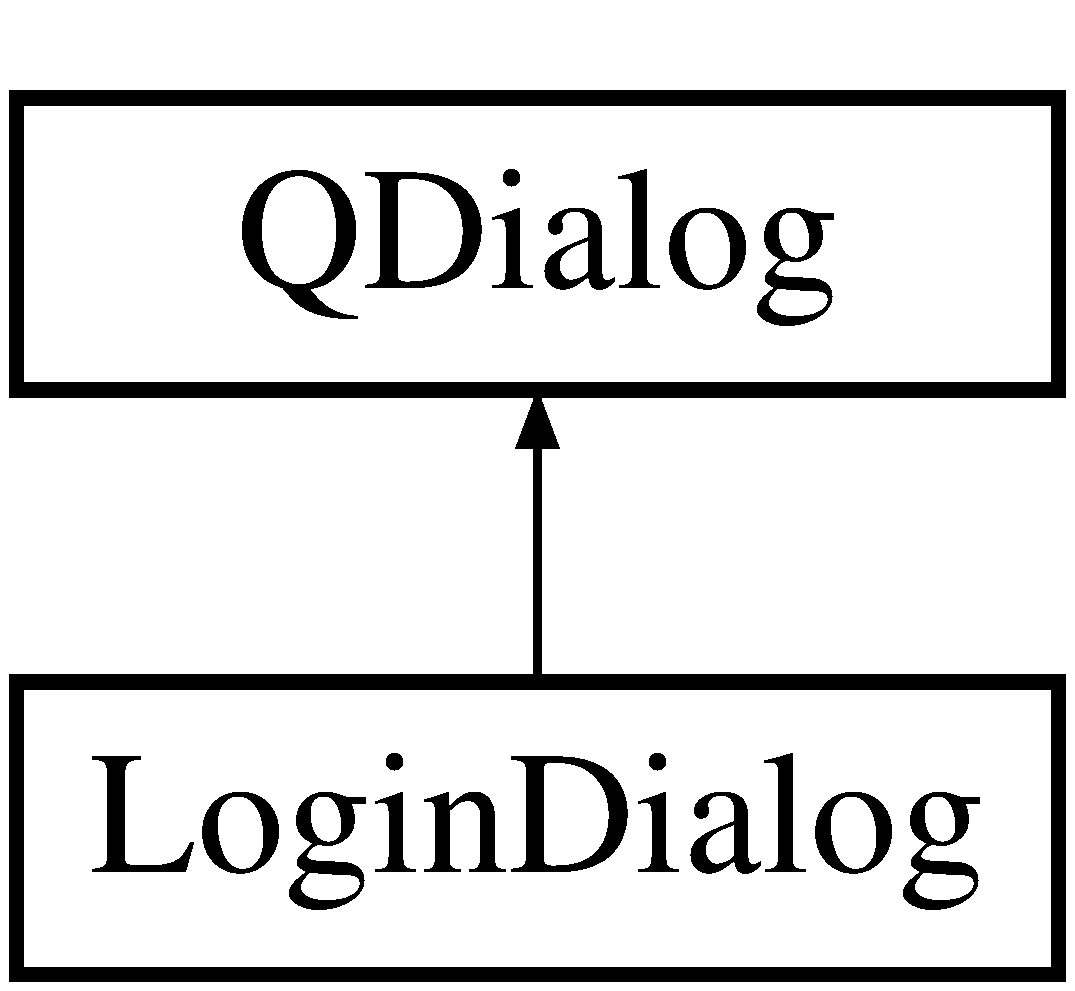
\includegraphics[height=2.000000cm]{classLoginDialog}
\end{center}
\end{figure}
\subsection*{Public Member Functions}
\begin{DoxyCompactItemize}
\item 
\hyperlink{classLoginDialog_af231bf82d3c72985f62bb47067255f47}{Login\-Dialog} (Q\-Widget $\ast$parent=0)
\item 
\hyperlink{classLoginDialog_aa5d012ebc424713ca0cbd82be1f81133}{$\sim$\-Login\-Dialog} ()
\end{DoxyCompactItemize}


\subsection{Constructor \& Destructor Documentation}
\hypertarget{classLoginDialog_af231bf82d3c72985f62bb47067255f47}{\index{Login\-Dialog@{Login\-Dialog}!Login\-Dialog@{Login\-Dialog}}
\index{Login\-Dialog@{Login\-Dialog}!LoginDialog@{Login\-Dialog}}
\subsubsection[{Login\-Dialog}]{\setlength{\rightskip}{0pt plus 5cm}Login\-Dialog\-::\-Login\-Dialog (
\begin{DoxyParamCaption}
\item[{Q\-Widget $\ast$}]{parent = {\ttfamily 0}}
\end{DoxyParamCaption}
)\hspace{0.3cm}{\ttfamily [explicit]}}}\label{classLoginDialog_af231bf82d3c72985f62bb47067255f47}

\begin{DoxyCode}
7                                         :
8     QDialog(parent),
9     ui(\textcolor{keyword}{new} Ui::LoginDialog)
10 \{
11     ui->setupUi(\textcolor{keyword}{this});
12 \}
\end{DoxyCode}
\hypertarget{classLoginDialog_aa5d012ebc424713ca0cbd82be1f81133}{\index{Login\-Dialog@{Login\-Dialog}!$\sim$\-Login\-Dialog@{$\sim$\-Login\-Dialog}}
\index{$\sim$\-Login\-Dialog@{$\sim$\-Login\-Dialog}!LoginDialog@{Login\-Dialog}}
\subsubsection[{$\sim$\-Login\-Dialog}]{\setlength{\rightskip}{0pt plus 5cm}Login\-Dialog\-::$\sim$\-Login\-Dialog (
\begin{DoxyParamCaption}
{}
\end{DoxyParamCaption}
)}}\label{classLoginDialog_aa5d012ebc424713ca0cbd82be1f81133}

\begin{DoxyCode}
15 \{
16     \textcolor{keyword}{delete} ui;
17 \}
\end{DoxyCode}


The documentation for this class was generated from the following files\-:\begin{DoxyCompactItemize}
\item 
\hyperlink{logindialog_8h}{logindialog.\-h}\item 
\hyperlink{logindialog_8cpp}{logindialog.\-cpp}\end{DoxyCompactItemize}

\hypertarget{classMainWindow}{\section{Main\-Window Class Reference}
\label{classMainWindow}\index{Main\-Window@{Main\-Window}}
}


{\ttfamily \#include $<$mainwindow.\-h$>$}

Inheritance diagram for Main\-Window\-:\begin{figure}[H]
\begin{center}
\leavevmode
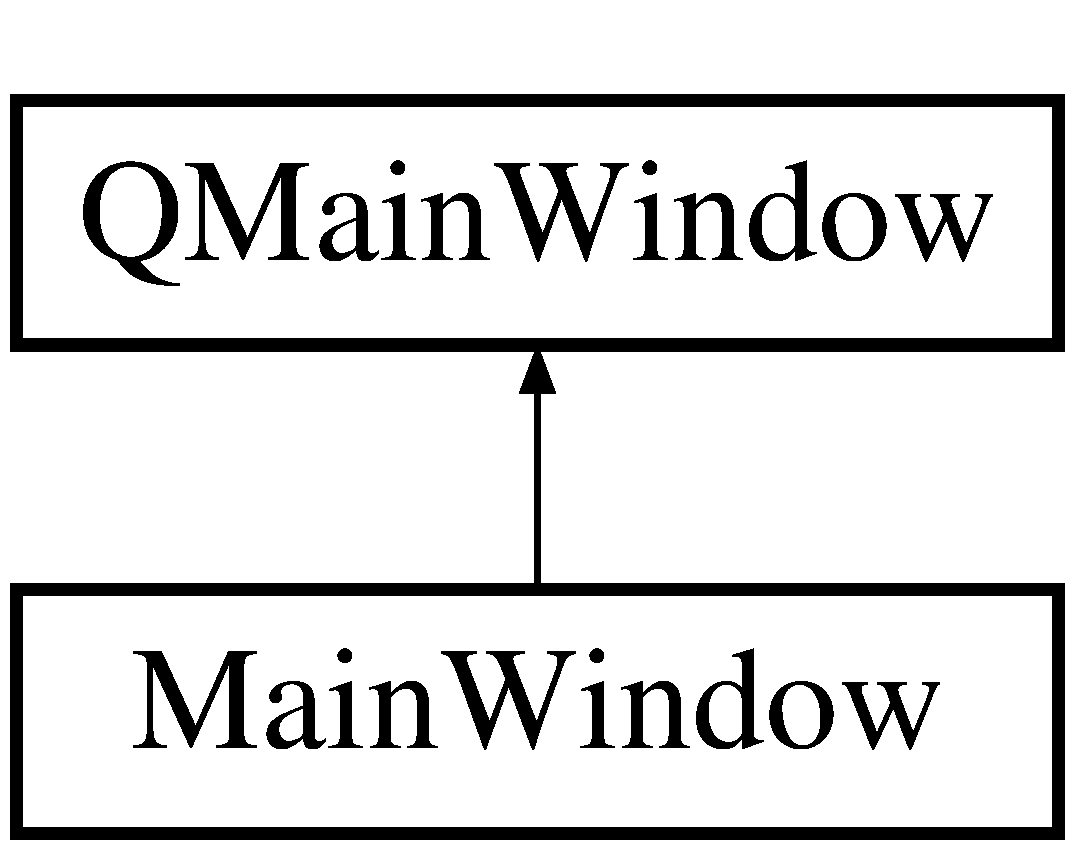
\includegraphics[height=2.000000cm]{classMainWindow}
\end{center}
\end{figure}
\subsection*{Public Slots}
\begin{DoxyCompactItemize}
\item 
void \hyperlink{classMainWindow_a2605ed0a3de91bd4e13316d16887fd60}{on\-\_\-b\-Send\-\_\-clicked} ()
\item 
void \hyperlink{classMainWindow_ab7ed8f9211b6a43151b645f94a019502}{received\-Message} (const char $\ast$)
\item 
void \hyperlink{classMainWindow_a9e94a105f93d43505bd528088fd23846}{received\-Message} (Q\-String response)
\item 
void \hyperlink{classMainWindow_ac2886ac3cabca51c9b4ff8643dfbeff8}{disconnect} ()
\item 
void \hyperlink{classMainWindow_a4358d0320935424d76a693791b1066f5}{open\-Server\-Properties} ()
\end{DoxyCompactItemize}
\subsection*{Public Member Functions}
\begin{DoxyCompactItemize}
\item 
\hyperlink{classMainWindow_a8b244be8b7b7db1b08de2a2acb9409db}{Main\-Window} (Q\-Widget $\ast$parent=0)
\item 
\hyperlink{classMainWindow_ae98d00a93bc118200eeef9f9bba1dba7}{$\sim$\-Main\-Window} ()
\end{DoxyCompactItemize}


\subsection{Constructor \& Destructor Documentation}
\hypertarget{classMainWindow_a8b244be8b7b7db1b08de2a2acb9409db}{\index{Main\-Window@{Main\-Window}!Main\-Window@{Main\-Window}}
\index{Main\-Window@{Main\-Window}!MainWindow@{Main\-Window}}
\subsubsection[{Main\-Window}]{\setlength{\rightskip}{0pt plus 5cm}Main\-Window\-::\-Main\-Window (
\begin{DoxyParamCaption}
\item[{Q\-Widget $\ast$}]{parent = {\ttfamily 0}}
\end{DoxyParamCaption}
)\hspace{0.3cm}{\ttfamily [explicit]}}}\label{classMainWindow_a8b244be8b7b7db1b08de2a2acb9409db}

\begin{DoxyCode}
15                                       :
16     QMainWindow(parent),
17     ui(\textcolor{keyword}{new} Ui::MainWindow)
18 \{
19     ui->setupUi(\textcolor{keyword}{this});
20     connect(ui->teCommand, SIGNAL(enterPressed()), \textcolor{keyword}{this}, SLOT(\hyperlink{classMainWindow_a2605ed0a3de91bd4e13316d16887fd60}{on\_bSend\_clicked}()));
21     this->server\_properties = \textcolor{keyword}{new} \hyperlink{classServerPropertiesDialog}{ServerPropertiesDialog}(\textcolor{keyword}{this});
22 
23     ui->teCommand->selectAll();
24     connect(ui->actionServer\_Properties, SIGNAL(triggered()), \textcolor{keyword}{this}, SLOT(
      \hyperlink{classMainWindow_a4358d0320935424d76a693791b1066f5}{openServerProperties}()));
25 
26     m\_server\_address.\hyperlink{classAddress_a43ba5f8001b7e729b83b1b9299294495}{setAddress}(server\_properties->\hyperlink{classServerPropertiesDialog_ae2fe6ffc4e0c04a9043a14a96f6aa5e9}{getHostName}().toStdString());
27     m\_server\_address.\hyperlink{classAddress_ad73c29200f7d63641e48ebfc16efaf75}{setPort}(server\_properties->\hyperlink{classServerPropertiesDialog_a00869f1fe5e8418017acfa6f351020d1}{getPort}());
28     \textcolor{comment}{//Try to set up the network connection}
29     m\_tcp\_interface = \textcolor{keyword}{new} \hyperlink{classNetworkToQtInterface}{NetworkToQtInterface}(m\_server\_address);
30     connect(m\_tcp\_interface, SIGNAL(messageDispatch(QString)), \textcolor{keyword}{this}, SLOT(
      \hyperlink{classMainWindow_ab7ed8f9211b6a43151b645f94a019502}{receivedMessage}(QString)));
31     connect(m\_tcp\_interface, SIGNAL(serverDisconnected()), \textcolor{keyword}{this}, SLOT(\hyperlink{classMainWindow_ac2886ac3cabca51c9b4ff8643dfbeff8}{disconnect}()));
32     this->setUpThreads();
33     \textcolor{comment}{//Delay server connect}
34 \textcolor{preprocessor}{#ifdef Q\_OS\_LINUX}
35 \textcolor{preprocessor}{}    \textcolor{comment}{//QTimer::singleShot(500, this, SLOT(delayServerConnect()));}
36 \textcolor{preprocessor}{#endif}
37 \textcolor{preprocessor}{}    QString q(\textcolor{stringliteral}{"Camera A"});
38 
39     vid = \textcolor{keyword}{new} \hyperlink{classVideoWindow}{VideoWindow}(\textcolor{keyword}{new} \hyperlink{classCamera}{Camera}(q, m\_server\_address, 
      \hyperlink{camera_8h_a10395294162cb49637e9c8f6efdb10eaa8845b57cef431c1017ee723500b2d1f5}{CONTENT\_TYPE\_PERSONAL}));
40     vid->setAttribute(Qt::WA\_DeleteOnClose);
41     vid->show();
42     \textcolor{comment}{//FOR UDP}
43     \textcolor{comment}{//Set up a packet sender thread}
44     \textcolor{comment}{//this->sender\_thread = new PacketSender();}
45     \textcolor{comment}{//Set up a packet receiver thread and execute for the life of the main window}
46     \textcolor{comment}{//this->receiver\_thread = new PacketReceiver(&m\_messageDispatcher);}
47     \textcolor{comment}{//this->receiver\_thread->start();}
48     \textcolor{comment}{//Connect receivers received signal to our slot}
49     \textcolor{comment}{//connect(&m\_messageDispatcher, SIGNAL(passMessage(const char *)), this, SLOT(receivedMessage(const
       char *)));}
50 \}
\end{DoxyCode}
\hypertarget{classMainWindow_ae98d00a93bc118200eeef9f9bba1dba7}{\index{Main\-Window@{Main\-Window}!$\sim$\-Main\-Window@{$\sim$\-Main\-Window}}
\index{$\sim$\-Main\-Window@{$\sim$\-Main\-Window}!MainWindow@{Main\-Window}}
\subsubsection[{$\sim$\-Main\-Window}]{\setlength{\rightskip}{0pt plus 5cm}Main\-Window\-::$\sim$\-Main\-Window (
\begin{DoxyParamCaption}
{}
\end{DoxyParamCaption}
)}}\label{classMainWindow_ae98d00a93bc118200eeef9f9bba1dba7}

\begin{DoxyCode}
53 \{
54     \textcolor{keyword}{delete} ui;
55     m\_request\_thread->terminate();
56     \textcolor{keyword}{delete} m\_tcp\_interface;
57 
58     \textcolor{keyword}{delete} m\_request\_thread;
59     \textcolor{keyword}{delete} server\_properties;
60 
61 
62     \textcolor{comment}{//For UDP}
63     \textcolor{comment}{//delete sender\_thread;}
64     \textcolor{comment}{//receiver\_thread->waitToFinish();}
65     \textcolor{comment}{//delete receiver\_thread;}
66 
67 \}
\end{DoxyCode}


\subsection{Member Function Documentation}
\hypertarget{classMainWindow_ac2886ac3cabca51c9b4ff8643dfbeff8}{\index{Main\-Window@{Main\-Window}!disconnect@{disconnect}}
\index{disconnect@{disconnect}!MainWindow@{Main\-Window}}
\subsubsection[{disconnect}]{\setlength{\rightskip}{0pt plus 5cm}void Main\-Window\-::disconnect (
\begin{DoxyParamCaption}
{}
\end{DoxyParamCaption}
)\hspace{0.3cm}{\ttfamily [slot]}}}\label{classMainWindow_ac2886ac3cabca51c9b4ff8643dfbeff8}

\begin{DoxyCode}
228 \{
229     m\_tcp\_interface->\hyperlink{classNetworkToQtInterface_ac4889eb9f3c5b5e4509252481335200f}{close}();
230     this->ui->bConnect->setText(\textcolor{stringliteral}{"Connect"});
231 \}
\end{DoxyCode}
\hypertarget{classMainWindow_a2605ed0a3de91bd4e13316d16887fd60}{\index{Main\-Window@{Main\-Window}!on\-\_\-b\-Send\-\_\-clicked@{on\-\_\-b\-Send\-\_\-clicked}}
\index{on\-\_\-b\-Send\-\_\-clicked@{on\-\_\-b\-Send\-\_\-clicked}!MainWindow@{Main\-Window}}
\subsubsection[{on\-\_\-b\-Send\-\_\-clicked}]{\setlength{\rightskip}{0pt plus 5cm}void Main\-Window\-::on\-\_\-b\-Send\-\_\-clicked (
\begin{DoxyParamCaption}
{}
\end{DoxyParamCaption}
)\hspace{0.3cm}{\ttfamily [slot]}}}\label{classMainWindow_a2605ed0a3de91bd4e13316d16887fd60}

\begin{DoxyCode}
82 \{
83     \hyperlink{Log_8h_a7cec51f4ce4b22e8c0f256485d57fca7}{INFO}() << \textcolor{stringliteral}{"Send button clicked."};
84     \textcolor{comment}{//Check to see if conencted to server}
85 \textcolor{comment}{//    if(!m\_tcp\_interface->isConnected())}
86 \textcolor{comment}{//    \{}
87 \textcolor{comment}{//        this->receivedMessage("Not connected to the server");}
88 \textcolor{comment}{//        return;}
89 \textcolor{comment}{//    \}}
90     \textcolor{comment}{//Send the command in the text box}
91     QString cmd = ui->teCommand->toPlainText();
92     \textcolor{comment}{//Send packet with text edit string as const char *}
93     std::string c\_cmd = cmd.toStdString();
94 
95     \textcolor{comment}{//Add command to list of previous commands}
96     \textcolor{keywordflow}{if}(c\_cmd.compare(\textcolor{stringliteral}{""}) != 0)
97     \{
98         ui->teCommand->addCommandToList(c\_cmd);
99     \}
100 
101     ui->teCommand->setText(\textcolor{stringliteral}{""});
102 
103     \textcolor{comment}{//ui->video\_container->playUrl(cmd);}
104     vid->\hyperlink{classVideoWindow_ac71a3e790d6956a26369294d5fb36c93}{streamVideo}(cmd);
105 
106     \textcolor{comment}{//cmd = cmd.trimmed();}
107     \textcolor{keywordflow}{if}(!cmd.isEmpty())
108         this->sendRequest(cmd);
109 
110     \textcolor{comment}{//FOR UDP}
111 
112     \textcolor{comment}{//Send packet last to protect data integrity}
113     \textcolor{comment}{//this->sendPacket(c\_cmd.c\_str());}
114     \textcolor{comment}{//Receive any responses from the other end}
115     \textcolor{comment}{//this->listenForPackets();}
116 
117 \}
\end{DoxyCode}
\hypertarget{classMainWindow_a4358d0320935424d76a693791b1066f5}{\index{Main\-Window@{Main\-Window}!open\-Server\-Properties@{open\-Server\-Properties}}
\index{open\-Server\-Properties@{open\-Server\-Properties}!MainWindow@{Main\-Window}}
\subsubsection[{open\-Server\-Properties}]{\setlength{\rightskip}{0pt plus 5cm}void Main\-Window\-::open\-Server\-Properties (
\begin{DoxyParamCaption}
{}
\end{DoxyParamCaption}
)\hspace{0.3cm}{\ttfamily [slot]}}}\label{classMainWindow_a4358d0320935424d76a693791b1066f5}

\begin{DoxyCode}
145 \{
146     server\_properties->show();
147     \textcolor{keywordtype}{int} ret = server\_properties->exec();
148     \textcolor{comment}{//See what the return value is}
149     \textcolor{keywordflow}{switch}(ret)
150     \{
151     \textcolor{keywordflow}{case} QDialog::Accepted:
152         \textcolor{comment}{//Update the address info}
153         m\_server\_address.\hyperlink{classAddress_a43ba5f8001b7e729b83b1b9299294495}{setAddress}(server\_properties->\hyperlink{classServerPropertiesDialog_ae2fe6ffc4e0c04a9043a14a96f6aa5e9}{getHostName}().toStdString());
154         m\_server\_address.\hyperlink{classAddress_ad73c29200f7d63641e48ebfc16efaf75}{setPort}(server\_properties->\hyperlink{classServerPropertiesDialog_a00869f1fe5e8418017acfa6f351020d1}{getPort}());
155         m\_tcp\_interface->\hyperlink{classNetworkToQtInterface_aa1fc46b9d7bf2e5c219ff36808c555eb}{setServerAddress}(m\_server\_address);
156         \textcolor{keywordflow}{break};
157     \textcolor{keywordflow}{case} QDialog::Rejected:
158         \textcolor{keywordflow}{break};
159     \}
160 \}
\end{DoxyCode}
\hypertarget{classMainWindow_ab7ed8f9211b6a43151b645f94a019502}{\index{Main\-Window@{Main\-Window}!received\-Message@{received\-Message}}
\index{received\-Message@{received\-Message}!MainWindow@{Main\-Window}}
\subsubsection[{received\-Message}]{\setlength{\rightskip}{0pt plus 5cm}void Main\-Window\-::received\-Message (
\begin{DoxyParamCaption}
\item[{const char $\ast$}]{data}
\end{DoxyParamCaption}
)\hspace{0.3cm}{\ttfamily [slot]}}}\label{classMainWindow_ab7ed8f9211b6a43151b645f94a019502}

\begin{DoxyCode}
126 \{
127     \hyperlink{Log_8h_a7cec51f4ce4b22e8c0f256485d57fca7}{INFO}() << \textcolor{stringliteral}{"In slot \(\backslash\)'receivedPacket\(\backslash\)' Message:"} << data;
128     QMessageBox msgBox;
129     msgBox.setText(QString(data));
130     \textcolor{keywordtype}{int} ret = msgBox.exec();
131 \}
\end{DoxyCode}
\hypertarget{classMainWindow_a9e94a105f93d43505bd528088fd23846}{\index{Main\-Window@{Main\-Window}!received\-Message@{received\-Message}}
\index{received\-Message@{received\-Message}!MainWindow@{Main\-Window}}
\subsubsection[{received\-Message}]{\setlength{\rightskip}{0pt plus 5cm}void Main\-Window\-::received\-Message (
\begin{DoxyParamCaption}
\item[{Q\-String}]{response}
\end{DoxyParamCaption}
)\hspace{0.3cm}{\ttfamily [slot]}}}\label{classMainWindow_a9e94a105f93d43505bd528088fd23846}

\begin{DoxyCode}
135 \{
136     \hyperlink{Log_8h_a7cec51f4ce4b22e8c0f256485d57fca7}{INFO}() << \textcolor{stringliteral}{"In slot \(\backslash\)'receivedPacket\(\backslash\)' Message:"} << response;
137     QMessageBox msgBox;
138     msgBox.setText(response);
139     \textcolor{keywordtype}{int} ret = msgBox.exec();
140 \}
\end{DoxyCode}


The documentation for this class was generated from the following files\-:\begin{DoxyCompactItemize}
\item 
\hyperlink{mainwindow_8h}{mainwindow.\-h}\item 
\hyperlink{mainwindow_8cpp}{mainwindow.\-cpp}\end{DoxyCompactItemize}

\hypertarget{classMediaStatistics}{\section{Media\-Statistics Class Reference}
\label{classMediaStatistics}\index{Media\-Statistics@{Media\-Statistics}}
}


A wrapper to V\-L\-C libvlc\-\_\-media\-\_\-stats\-\_\-t struct.  




{\ttfamily \#include $<$mediastatistics.\-h$>$}

\subsection*{Public Member Functions}
\begin{DoxyCompactItemize}
\item 
\hyperlink{classMediaStatistics_a5b768a2e4c481a3e630ea88f1d7e6540}{Media\-Statistics} ()
\begin{DoxyCompactList}\small\item\em \hyperlink{classMediaStatistics}{Media\-Statistics} constructor. \end{DoxyCompactList}\item 
int \hyperlink{classMediaStatistics_a93b33f4ac072547f33b6a5be0d47f1d2}{get\-Read\-Bytes} () const 
\item 
void \hyperlink{classMediaStatistics_a729d2733cd49ad96ab595bb5eb38fe87}{set\-Read\-Bytes} (int value)
\item 
int \hyperlink{classMediaStatistics_ac48baa2b782e0dbcadd5d69914f9e80c}{get\-Demux\-Read\-Bytes} () const 
\item 
void \hyperlink{classMediaStatistics_afecbd2e8ebc147b344a9dc18dc6af431}{set\-Demux\-Read\-Bytes} (int value)
\item 
int \hyperlink{classMediaStatistics_aaa080505dbe504d5a4d696f4cbaf989d}{get\-Demux\-Corrupted} () const 
\item 
void \hyperlink{classMediaStatistics_a6d9b5760c321c9e189c780ad64cda8f8}{set\-Demux\-Corrupted} (int value)
\item 
int \hyperlink{classMediaStatistics_ad3c91e75dd165e0ca308dc40990ecc87}{get\-Demux\-Discontinuity} () const 
\item 
void \hyperlink{classMediaStatistics_a05b13c332cd4ed139392e528b52ac89c}{set\-Demux\-Discontinuity} (int value)
\item 
int \hyperlink{classMediaStatistics_a5265392ca4db34bf23cf298e8fd506af}{get\-Decoded\-Video} () const 
\item 
void \hyperlink{classMediaStatistics_a267abf187ab5690f931d0d7d45407dcc}{set\-Decoded\-Video} (int value)
\item 
int \hyperlink{classMediaStatistics_a2b1143b0060a9a21ba6ea5a881fa76c1}{get\-Displayed\-Pictures} () const 
\item 
void \hyperlink{classMediaStatistics_ad37d42721c420cea8862cbfd27380a69}{set\-Displayed\-Pictures} (int value)
\item 
int \hyperlink{classMediaStatistics_a1548c3da664b452a5c8ecbd927d7f684}{get\-Played\-Pictures} () const 
\item 
void \hyperlink{classMediaStatistics_adf378b9efe24da6724583ff13ad98356}{set\-Played\-Pictures} (int value)
\item 
int \hyperlink{classMediaStatistics_a264840500b7d487d6226e20b183c54ce}{get\-Lost\-Pictures} () const 
\item 
void \hyperlink{classMediaStatistics_a0b305cf428cdc7905d2beb98f08e7c62}{set\-Lost\-Pictures} (int value)
\item 
float \hyperlink{classMediaStatistics_a436b36f7f22c4bc93da33712c9e200f4}{get\-Input\-Bitrate} () const 
\item 
void \hyperlink{classMediaStatistics_ad504b337caf39ac04909a4c480101c19}{set\-Input\-Bitrate} (float value)
\item 
float \hyperlink{classMediaStatistics_a046962e0db08292a1778bb859c234908}{get\-Demux\-Bitrate} () const 
\item 
void \hyperlink{classMediaStatistics_a36bd398cacfada1aaf865374f4bc5e2a}{set\-Demux\-Bitrate} (float value)
\end{DoxyCompactItemize}


\subsection{Detailed Description}
A wrapper to V\-L\-C libvlc\-\_\-media\-\_\-stats\-\_\-t struct. 

This class serves as a C++ wrapper to the libvlc\-\_\-media\-\_\-stats\-\_\-t struct defined by V\-L\-C. It encapsulates only the fields we may be interested in. 

\subsection{Constructor \& Destructor Documentation}
\hypertarget{classMediaStatistics_a5b768a2e4c481a3e630ea88f1d7e6540}{\index{Media\-Statistics@{Media\-Statistics}!Media\-Statistics@{Media\-Statistics}}
\index{Media\-Statistics@{Media\-Statistics}!MediaStatistics@{Media\-Statistics}}
\subsubsection[{Media\-Statistics}]{\setlength{\rightskip}{0pt plus 5cm}Media\-Statistics\-::\-Media\-Statistics (
\begin{DoxyParamCaption}
{}
\end{DoxyParamCaption}
)}}\label{classMediaStatistics_a5b768a2e4c481a3e630ea88f1d7e6540}


\hyperlink{classMediaStatistics}{Media\-Statistics} constructor. 


\begin{DoxyCode}
4 \{
5 \}
\end{DoxyCode}


\subsection{Member Function Documentation}
\hypertarget{classMediaStatistics_a5265392ca4db34bf23cf298e8fd506af}{\index{Media\-Statistics@{Media\-Statistics}!get\-Decoded\-Video@{get\-Decoded\-Video}}
\index{get\-Decoded\-Video@{get\-Decoded\-Video}!MediaStatistics@{Media\-Statistics}}
\subsubsection[{get\-Decoded\-Video}]{\setlength{\rightskip}{0pt plus 5cm}int Media\-Statistics\-::get\-Decoded\-Video (
\begin{DoxyParamCaption}
{}
\end{DoxyParamCaption}
) const}}\label{classMediaStatistics_a5265392ca4db34bf23cf298e8fd506af}

\begin{DoxyCode}
58 \{
59     \textcolor{keywordflow}{return} decodedVideo;
60 \}
\end{DoxyCode}
\hypertarget{classMediaStatistics_a046962e0db08292a1778bb859c234908}{\index{Media\-Statistics@{Media\-Statistics}!get\-Demux\-Bitrate@{get\-Demux\-Bitrate}}
\index{get\-Demux\-Bitrate@{get\-Demux\-Bitrate}!MediaStatistics@{Media\-Statistics}}
\subsubsection[{get\-Demux\-Bitrate}]{\setlength{\rightskip}{0pt plus 5cm}float Media\-Statistics\-::get\-Demux\-Bitrate (
\begin{DoxyParamCaption}
{}
\end{DoxyParamCaption}
) const}}\label{classMediaStatistics_a046962e0db08292a1778bb859c234908}

\begin{DoxyCode}
8 \{
9     \textcolor{keywordflow}{return} demuxBitrate;
10 \}
\end{DoxyCode}
\hypertarget{classMediaStatistics_aaa080505dbe504d5a4d696f4cbaf989d}{\index{Media\-Statistics@{Media\-Statistics}!get\-Demux\-Corrupted@{get\-Demux\-Corrupted}}
\index{get\-Demux\-Corrupted@{get\-Demux\-Corrupted}!MediaStatistics@{Media\-Statistics}}
\subsubsection[{get\-Demux\-Corrupted}]{\setlength{\rightskip}{0pt plus 5cm}int Media\-Statistics\-::get\-Demux\-Corrupted (
\begin{DoxyParamCaption}
{}
\end{DoxyParamCaption}
) const}}\label{classMediaStatistics_aaa080505dbe504d5a4d696f4cbaf989d}

\begin{DoxyCode}
78 \{
79     \textcolor{keywordflow}{return} demuxCorrupted;
80 \}
\end{DoxyCode}
\hypertarget{classMediaStatistics_ad3c91e75dd165e0ca308dc40990ecc87}{\index{Media\-Statistics@{Media\-Statistics}!get\-Demux\-Discontinuity@{get\-Demux\-Discontinuity}}
\index{get\-Demux\-Discontinuity@{get\-Demux\-Discontinuity}!MediaStatistics@{Media\-Statistics}}
\subsubsection[{get\-Demux\-Discontinuity}]{\setlength{\rightskip}{0pt plus 5cm}int Media\-Statistics\-::get\-Demux\-Discontinuity (
\begin{DoxyParamCaption}
{}
\end{DoxyParamCaption}
) const}}\label{classMediaStatistics_ad3c91e75dd165e0ca308dc40990ecc87}

\begin{DoxyCode}
68 \{
69     \textcolor{keywordflow}{return} demuxDiscontinuity;
70 \}
\end{DoxyCode}
\hypertarget{classMediaStatistics_ac48baa2b782e0dbcadd5d69914f9e80c}{\index{Media\-Statistics@{Media\-Statistics}!get\-Demux\-Read\-Bytes@{get\-Demux\-Read\-Bytes}}
\index{get\-Demux\-Read\-Bytes@{get\-Demux\-Read\-Bytes}!MediaStatistics@{Media\-Statistics}}
\subsubsection[{get\-Demux\-Read\-Bytes}]{\setlength{\rightskip}{0pt plus 5cm}int Media\-Statistics\-::get\-Demux\-Read\-Bytes (
\begin{DoxyParamCaption}
{}
\end{DoxyParamCaption}
) const}}\label{classMediaStatistics_ac48baa2b782e0dbcadd5d69914f9e80c}

\begin{DoxyCode}
88 \{
89     \textcolor{keywordflow}{return} demuxReadBytes;
90 \}
\end{DoxyCode}
\hypertarget{classMediaStatistics_a2b1143b0060a9a21ba6ea5a881fa76c1}{\index{Media\-Statistics@{Media\-Statistics}!get\-Displayed\-Pictures@{get\-Displayed\-Pictures}}
\index{get\-Displayed\-Pictures@{get\-Displayed\-Pictures}!MediaStatistics@{Media\-Statistics}}
\subsubsection[{get\-Displayed\-Pictures}]{\setlength{\rightskip}{0pt plus 5cm}int Media\-Statistics\-::get\-Displayed\-Pictures (
\begin{DoxyParamCaption}
{}
\end{DoxyParamCaption}
) const}}\label{classMediaStatistics_a2b1143b0060a9a21ba6ea5a881fa76c1}

\begin{DoxyCode}
48 \{
49     \textcolor{keywordflow}{return} displayedPictures;
50 \}
\end{DoxyCode}
\hypertarget{classMediaStatistics_a436b36f7f22c4bc93da33712c9e200f4}{\index{Media\-Statistics@{Media\-Statistics}!get\-Input\-Bitrate@{get\-Input\-Bitrate}}
\index{get\-Input\-Bitrate@{get\-Input\-Bitrate}!MediaStatistics@{Media\-Statistics}}
\subsubsection[{get\-Input\-Bitrate}]{\setlength{\rightskip}{0pt plus 5cm}float Media\-Statistics\-::get\-Input\-Bitrate (
\begin{DoxyParamCaption}
{}
\end{DoxyParamCaption}
) const}}\label{classMediaStatistics_a436b36f7f22c4bc93da33712c9e200f4}

\begin{DoxyCode}
18 \{
19     \textcolor{keywordflow}{return} inputBitrate;
20 \}
\end{DoxyCode}
\hypertarget{classMediaStatistics_a264840500b7d487d6226e20b183c54ce}{\index{Media\-Statistics@{Media\-Statistics}!get\-Lost\-Pictures@{get\-Lost\-Pictures}}
\index{get\-Lost\-Pictures@{get\-Lost\-Pictures}!MediaStatistics@{Media\-Statistics}}
\subsubsection[{get\-Lost\-Pictures}]{\setlength{\rightskip}{0pt plus 5cm}int Media\-Statistics\-::get\-Lost\-Pictures (
\begin{DoxyParamCaption}
{}
\end{DoxyParamCaption}
) const}}\label{classMediaStatistics_a264840500b7d487d6226e20b183c54ce}

\begin{DoxyCode}
28 \{
29     \textcolor{keywordflow}{return} lostPictures;
30 \}
\end{DoxyCode}
\hypertarget{classMediaStatistics_a1548c3da664b452a5c8ecbd927d7f684}{\index{Media\-Statistics@{Media\-Statistics}!get\-Played\-Pictures@{get\-Played\-Pictures}}
\index{get\-Played\-Pictures@{get\-Played\-Pictures}!MediaStatistics@{Media\-Statistics}}
\subsubsection[{get\-Played\-Pictures}]{\setlength{\rightskip}{0pt plus 5cm}int Media\-Statistics\-::get\-Played\-Pictures (
\begin{DoxyParamCaption}
{}
\end{DoxyParamCaption}
) const}}\label{classMediaStatistics_a1548c3da664b452a5c8ecbd927d7f684}

\begin{DoxyCode}
38 \{
39     \textcolor{keywordflow}{return} playedPictures;
40 \}
\end{DoxyCode}
\hypertarget{classMediaStatistics_a93b33f4ac072547f33b6a5be0d47f1d2}{\index{Media\-Statistics@{Media\-Statistics}!get\-Read\-Bytes@{get\-Read\-Bytes}}
\index{get\-Read\-Bytes@{get\-Read\-Bytes}!MediaStatistics@{Media\-Statistics}}
\subsubsection[{get\-Read\-Bytes}]{\setlength{\rightskip}{0pt plus 5cm}int Media\-Statistics\-::get\-Read\-Bytes (
\begin{DoxyParamCaption}
{}
\end{DoxyParamCaption}
) const}}\label{classMediaStatistics_a93b33f4ac072547f33b6a5be0d47f1d2}

\begin{DoxyCode}
98 \{
99     \textcolor{keywordflow}{return} readBytes;
100 \}
\end{DoxyCode}
\hypertarget{classMediaStatistics_a267abf187ab5690f931d0d7d45407dcc}{\index{Media\-Statistics@{Media\-Statistics}!set\-Decoded\-Video@{set\-Decoded\-Video}}
\index{set\-Decoded\-Video@{set\-Decoded\-Video}!MediaStatistics@{Media\-Statistics}}
\subsubsection[{set\-Decoded\-Video}]{\setlength{\rightskip}{0pt plus 5cm}void Media\-Statistics\-::set\-Decoded\-Video (
\begin{DoxyParamCaption}
\item[{int}]{value}
\end{DoxyParamCaption}
)}}\label{classMediaStatistics_a267abf187ab5690f931d0d7d45407dcc}

\begin{DoxyCode}
63 \{
64     decodedVideo = value;
65 \}
\end{DoxyCode}
\hypertarget{classMediaStatistics_a36bd398cacfada1aaf865374f4bc5e2a}{\index{Media\-Statistics@{Media\-Statistics}!set\-Demux\-Bitrate@{set\-Demux\-Bitrate}}
\index{set\-Demux\-Bitrate@{set\-Demux\-Bitrate}!MediaStatistics@{Media\-Statistics}}
\subsubsection[{set\-Demux\-Bitrate}]{\setlength{\rightskip}{0pt plus 5cm}void Media\-Statistics\-::set\-Demux\-Bitrate (
\begin{DoxyParamCaption}
\item[{float}]{value}
\end{DoxyParamCaption}
)}}\label{classMediaStatistics_a36bd398cacfada1aaf865374f4bc5e2a}

\begin{DoxyCode}
13 \{
14     demuxBitrate = value;
15 \}
\end{DoxyCode}
\hypertarget{classMediaStatistics_a6d9b5760c321c9e189c780ad64cda8f8}{\index{Media\-Statistics@{Media\-Statistics}!set\-Demux\-Corrupted@{set\-Demux\-Corrupted}}
\index{set\-Demux\-Corrupted@{set\-Demux\-Corrupted}!MediaStatistics@{Media\-Statistics}}
\subsubsection[{set\-Demux\-Corrupted}]{\setlength{\rightskip}{0pt plus 5cm}void Media\-Statistics\-::set\-Demux\-Corrupted (
\begin{DoxyParamCaption}
\item[{int}]{value}
\end{DoxyParamCaption}
)}}\label{classMediaStatistics_a6d9b5760c321c9e189c780ad64cda8f8}

\begin{DoxyCode}
83 \{
84     demuxCorrupted = value;
85 \}
\end{DoxyCode}
\hypertarget{classMediaStatistics_a05b13c332cd4ed139392e528b52ac89c}{\index{Media\-Statistics@{Media\-Statistics}!set\-Demux\-Discontinuity@{set\-Demux\-Discontinuity}}
\index{set\-Demux\-Discontinuity@{set\-Demux\-Discontinuity}!MediaStatistics@{Media\-Statistics}}
\subsubsection[{set\-Demux\-Discontinuity}]{\setlength{\rightskip}{0pt plus 5cm}void Media\-Statistics\-::set\-Demux\-Discontinuity (
\begin{DoxyParamCaption}
\item[{int}]{value}
\end{DoxyParamCaption}
)}}\label{classMediaStatistics_a05b13c332cd4ed139392e528b52ac89c}

\begin{DoxyCode}
73 \{
74     demuxDiscontinuity = value;
75 \}
\end{DoxyCode}
\hypertarget{classMediaStatistics_afecbd2e8ebc147b344a9dc18dc6af431}{\index{Media\-Statistics@{Media\-Statistics}!set\-Demux\-Read\-Bytes@{set\-Demux\-Read\-Bytes}}
\index{set\-Demux\-Read\-Bytes@{set\-Demux\-Read\-Bytes}!MediaStatistics@{Media\-Statistics}}
\subsubsection[{set\-Demux\-Read\-Bytes}]{\setlength{\rightskip}{0pt plus 5cm}void Media\-Statistics\-::set\-Demux\-Read\-Bytes (
\begin{DoxyParamCaption}
\item[{int}]{value}
\end{DoxyParamCaption}
)}}\label{classMediaStatistics_afecbd2e8ebc147b344a9dc18dc6af431}

\begin{DoxyCode}
93 \{
94     demuxReadBytes = value;
95 \}
\end{DoxyCode}
\hypertarget{classMediaStatistics_ad37d42721c420cea8862cbfd27380a69}{\index{Media\-Statistics@{Media\-Statistics}!set\-Displayed\-Pictures@{set\-Displayed\-Pictures}}
\index{set\-Displayed\-Pictures@{set\-Displayed\-Pictures}!MediaStatistics@{Media\-Statistics}}
\subsubsection[{set\-Displayed\-Pictures}]{\setlength{\rightskip}{0pt plus 5cm}void Media\-Statistics\-::set\-Displayed\-Pictures (
\begin{DoxyParamCaption}
\item[{int}]{value}
\end{DoxyParamCaption}
)}}\label{classMediaStatistics_ad37d42721c420cea8862cbfd27380a69}

\begin{DoxyCode}
53 \{
54     displayedPictures = value;
55 \}
\end{DoxyCode}
\hypertarget{classMediaStatistics_ad504b337caf39ac04909a4c480101c19}{\index{Media\-Statistics@{Media\-Statistics}!set\-Input\-Bitrate@{set\-Input\-Bitrate}}
\index{set\-Input\-Bitrate@{set\-Input\-Bitrate}!MediaStatistics@{Media\-Statistics}}
\subsubsection[{set\-Input\-Bitrate}]{\setlength{\rightskip}{0pt plus 5cm}void Media\-Statistics\-::set\-Input\-Bitrate (
\begin{DoxyParamCaption}
\item[{float}]{value}
\end{DoxyParamCaption}
)}}\label{classMediaStatistics_ad504b337caf39ac04909a4c480101c19}

\begin{DoxyCode}
23 \{
24     inputBitrate = value;
25 \}
\end{DoxyCode}
\hypertarget{classMediaStatistics_a0b305cf428cdc7905d2beb98f08e7c62}{\index{Media\-Statistics@{Media\-Statistics}!set\-Lost\-Pictures@{set\-Lost\-Pictures}}
\index{set\-Lost\-Pictures@{set\-Lost\-Pictures}!MediaStatistics@{Media\-Statistics}}
\subsubsection[{set\-Lost\-Pictures}]{\setlength{\rightskip}{0pt plus 5cm}void Media\-Statistics\-::set\-Lost\-Pictures (
\begin{DoxyParamCaption}
\item[{int}]{value}
\end{DoxyParamCaption}
)}}\label{classMediaStatistics_a0b305cf428cdc7905d2beb98f08e7c62}

\begin{DoxyCode}
33 \{
34     lostPictures = value;
35 \}
\end{DoxyCode}
\hypertarget{classMediaStatistics_adf378b9efe24da6724583ff13ad98356}{\index{Media\-Statistics@{Media\-Statistics}!set\-Played\-Pictures@{set\-Played\-Pictures}}
\index{set\-Played\-Pictures@{set\-Played\-Pictures}!MediaStatistics@{Media\-Statistics}}
\subsubsection[{set\-Played\-Pictures}]{\setlength{\rightskip}{0pt plus 5cm}void Media\-Statistics\-::set\-Played\-Pictures (
\begin{DoxyParamCaption}
\item[{int}]{value}
\end{DoxyParamCaption}
)}}\label{classMediaStatistics_adf378b9efe24da6724583ff13ad98356}

\begin{DoxyCode}
43 \{
44     playedPictures = value;
45 \}
\end{DoxyCode}
\hypertarget{classMediaStatistics_a729d2733cd49ad96ab595bb5eb38fe87}{\index{Media\-Statistics@{Media\-Statistics}!set\-Read\-Bytes@{set\-Read\-Bytes}}
\index{set\-Read\-Bytes@{set\-Read\-Bytes}!MediaStatistics@{Media\-Statistics}}
\subsubsection[{set\-Read\-Bytes}]{\setlength{\rightskip}{0pt plus 5cm}void Media\-Statistics\-::set\-Read\-Bytes (
\begin{DoxyParamCaption}
\item[{int}]{value}
\end{DoxyParamCaption}
)}}\label{classMediaStatistics_a729d2733cd49ad96ab595bb5eb38fe87}

\begin{DoxyCode}
103 \{
104     readBytes = value;
105 \}
\end{DoxyCode}


The documentation for this class was generated from the following files\-:\begin{DoxyCompactItemize}
\item 
Types/\hyperlink{mediastatistics_8h}{mediastatistics.\-h}\item 
Types/\hyperlink{mediastatistics_8cpp}{mediastatistics.\-cpp}\end{DoxyCompactItemize}

\hypertarget{classMessageDispatcher}{\section{Message\-Dispatcher Class Reference}
\label{classMessageDispatcher}\index{Message\-Dispatcher@{Message\-Dispatcher}}
}


{\ttfamily \#include $<$messagedispatcher.\-h$>$}

Inheritance diagram for Message\-Dispatcher\-:\begin{figure}[H]
\begin{center}
\leavevmode
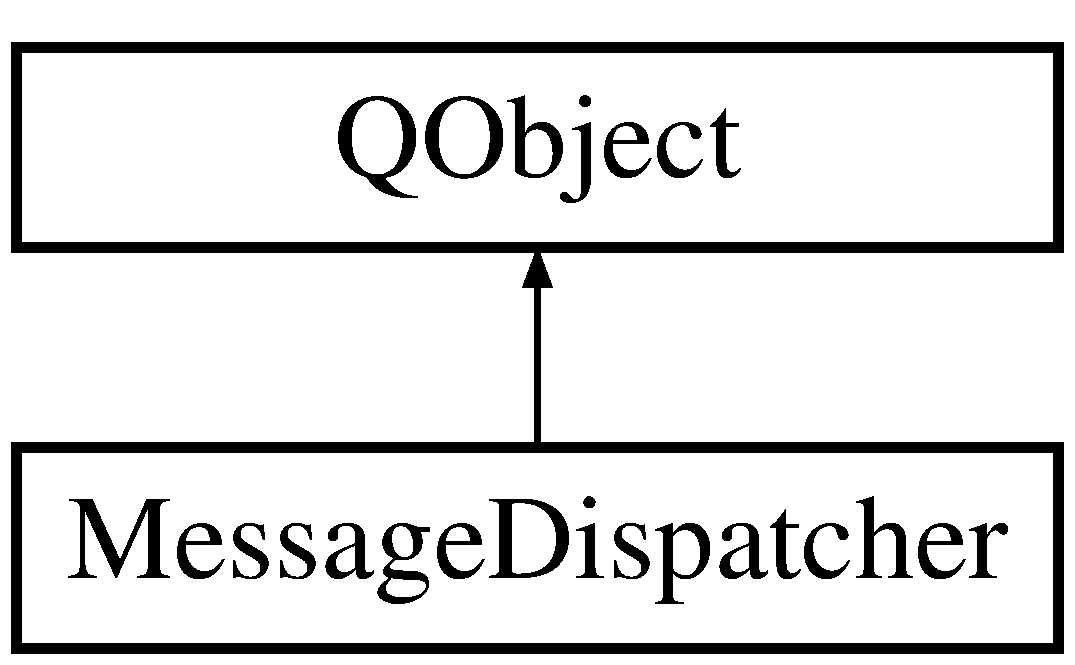
\includegraphics[height=2.000000cm]{classMessageDispatcher}
\end{center}
\end{figure}
\subsection*{Signals}
\begin{DoxyCompactItemize}
\item 
void \hyperlink{classMessageDispatcher_aae3af7ebcc73f9600a9ed2ba7682852e}{pass\-Message} (const char $\ast$)
\end{DoxyCompactItemize}
\subsection*{Public Member Functions}
\begin{DoxyCompactItemize}
\item 
\hyperlink{classMessageDispatcher_a9317eb6dd92c7a4c4a7b83ef87e4f11f}{Message\-Dispatcher} ()
\item 
void \hyperlink{classMessageDispatcher_a5c3f81bf5d598bb5f3833ef0d6e140a7}{reemit\-Message} (const char $\ast$msg)
\end{DoxyCompactItemize}


\subsection{Constructor \& Destructor Documentation}
\hypertarget{classMessageDispatcher_a9317eb6dd92c7a4c4a7b83ef87e4f11f}{\index{Message\-Dispatcher@{Message\-Dispatcher}!Message\-Dispatcher@{Message\-Dispatcher}}
\index{Message\-Dispatcher@{Message\-Dispatcher}!MessageDispatcher@{Message\-Dispatcher}}
\subsubsection[{Message\-Dispatcher}]{\setlength{\rightskip}{0pt plus 5cm}Message\-Dispatcher\-::\-Message\-Dispatcher (
\begin{DoxyParamCaption}
{}
\end{DoxyParamCaption}
)}}\label{classMessageDispatcher_a9317eb6dd92c7a4c4a7b83ef87e4f11f}

\begin{DoxyCode}
4 \{
5 \}
\end{DoxyCode}


\subsection{Member Function Documentation}
\hypertarget{classMessageDispatcher_aae3af7ebcc73f9600a9ed2ba7682852e}{\index{Message\-Dispatcher@{Message\-Dispatcher}!pass\-Message@{pass\-Message}}
\index{pass\-Message@{pass\-Message}!MessageDispatcher@{Message\-Dispatcher}}
\subsubsection[{pass\-Message}]{\setlength{\rightskip}{0pt plus 5cm}void Message\-Dispatcher\-::pass\-Message (
\begin{DoxyParamCaption}
\item[{const char $\ast$}]{}
\end{DoxyParamCaption}
)\hspace{0.3cm}{\ttfamily [signal]}}}\label{classMessageDispatcher_aae3af7ebcc73f9600a9ed2ba7682852e}
\hypertarget{classMessageDispatcher_a5c3f81bf5d598bb5f3833ef0d6e140a7}{\index{Message\-Dispatcher@{Message\-Dispatcher}!reemit\-Message@{reemit\-Message}}
\index{reemit\-Message@{reemit\-Message}!MessageDispatcher@{Message\-Dispatcher}}
\subsubsection[{reemit\-Message}]{\setlength{\rightskip}{0pt plus 5cm}void Message\-Dispatcher\-::reemit\-Message (
\begin{DoxyParamCaption}
\item[{const char $\ast$}]{msg}
\end{DoxyParamCaption}
)}}\label{classMessageDispatcher_a5c3f81bf5d598bb5f3833ef0d6e140a7}

\begin{DoxyCode}
8 \{
9     emit \hyperlink{classMessageDispatcher_aae3af7ebcc73f9600a9ed2ba7682852e}{passMessage}(msg);
10 \}
\end{DoxyCode}


The documentation for this class was generated from the following files\-:\begin{DoxyCompactItemize}
\item 
Util/\hyperlink{messagedispatcher_8h}{messagedispatcher.\-h}\item 
Util/\hyperlink{messagedispatcher_8cpp}{messagedispatcher.\-cpp}\end{DoxyCompactItemize}

\hypertarget{structnamespace__uri__predicate}{\section{namespace\-\_\-uri\-\_\-predicate Struct Reference}
\label{structnamespace__uri__predicate}\index{namespace\-\_\-uri\-\_\-predicate@{namespace\-\_\-uri\-\_\-predicate}}
}
\subsection*{Public Member Functions}
\begin{DoxyCompactItemize}
\item 
\hyperlink{structnamespace__uri__predicate_a25bef9c1e12b0fdc908275ae7ab7c202}{namespace\-\_\-uri\-\_\-predicate} (const char\-\_\-t $\ast$name)
\item 
bool \hyperlink{structnamespace__uri__predicate_ab4580e45d603d3eedfe75fec74210ce1}{operator()} (const xml\-\_\-attribute \&a) const 
\end{DoxyCompactItemize}
\subsection*{Data Fields}
\begin{DoxyCompactItemize}
\item 
const char\-\_\-t $\ast$ \hyperlink{structnamespace__uri__predicate_a80a2c051b9e57b8895c28d8fcc32e051}{prefix}
\item 
size\-\_\-t \hyperlink{structnamespace__uri__predicate_aa48279192e8d48b9c798f5485a2a9170}{prefix\-\_\-length}
\end{DoxyCompactItemize}


\subsection{Constructor \& Destructor Documentation}
\hypertarget{structnamespace__uri__predicate_a25bef9c1e12b0fdc908275ae7ab7c202}{\index{namespace\-\_\-uri\-\_\-predicate@{namespace\-\_\-uri\-\_\-predicate}!namespace\-\_\-uri\-\_\-predicate@{namespace\-\_\-uri\-\_\-predicate}}
\index{namespace\-\_\-uri\-\_\-predicate@{namespace\-\_\-uri\-\_\-predicate}!namespace_uri_predicate@{namespace\-\_\-uri\-\_\-predicate}}
\subsubsection[{namespace\-\_\-uri\-\_\-predicate}]{\setlength{\rightskip}{0pt plus 5cm}namespace\-\_\-uri\-\_\-predicate\-::namespace\-\_\-uri\-\_\-predicate (
\begin{DoxyParamCaption}
\item[{const char\-\_\-t $\ast$}]{name}
\end{DoxyParamCaption}
)\hspace{0.3cm}{\ttfamily [inline]}}}\label{structnamespace__uri__predicate_a25bef9c1e12b0fdc908275ae7ab7c202}

\begin{DoxyCode}
6495         \{
6496             \textcolor{keyword}{const} \hyperlink{namespacepugi_aef5a7a62cba0507542220ea15afe39df}{char\_t}* pos = \hyperlink{pugixml_8cpp_a490922f92ed98e972a13ffb410400a57}{find\_char}(name, \textcolor{charliteral}{':'});
6497 
6498             \hyperlink{structnamespace__uri__predicate_a80a2c051b9e57b8895c28d8fcc32e051}{prefix} = pos ? name : 0;
6499             \hyperlink{structnamespace__uri__predicate_aa48279192e8d48b9c798f5485a2a9170}{prefix\_length} = pos ? \textcolor{keyword}{static\_cast<}\textcolor{keywordtype}{size\_t}\textcolor{keyword}{>}(pos - name) : 0;
6500         \}
\end{DoxyCode}


\subsection{Member Function Documentation}
\hypertarget{structnamespace__uri__predicate_ab4580e45d603d3eedfe75fec74210ce1}{\index{namespace\-\_\-uri\-\_\-predicate@{namespace\-\_\-uri\-\_\-predicate}!operator()@{operator()}}
\index{operator()@{operator()}!namespace_uri_predicate@{namespace\-\_\-uri\-\_\-predicate}}
\subsubsection[{operator()}]{\setlength{\rightskip}{0pt plus 5cm}bool namespace\-\_\-uri\-\_\-predicate\-::operator() (
\begin{DoxyParamCaption}
\item[{const xml\-\_\-attribute \&}]{a}
\end{DoxyParamCaption}
) const\hspace{0.3cm}{\ttfamily [inline]}}}\label{structnamespace__uri__predicate_ab4580e45d603d3eedfe75fec74210ce1}

\begin{DoxyCode}
6503         \{
6504             \textcolor{keyword}{const} \hyperlink{namespacepugi_aef5a7a62cba0507542220ea15afe39df}{char\_t}* name = a.name();
6505 
6506             \textcolor{keywordflow}{if} (!\hyperlink{pugixml_8cpp_a4ab3a20f90bd9a6d4d050b7438fe83e3}{starts\_with}(name, \hyperlink{pugixml_8hpp_ad5475bca2e336810ae5906349e644d0b}{PUGIXML\_TEXT}(\textcolor{stringliteral}{"xmlns"}))) \textcolor{keywordflow}{return} \textcolor{keyword}{false};
6507 
6508             \textcolor{keywordflow}{return} \hyperlink{structnamespace__uri__predicate_a80a2c051b9e57b8895c28d8fcc32e051}{prefix} ? name[5] == \textcolor{charliteral}{':'} && \hyperlink{pugixml_8cpp_abbf171d1eb53f93f1fa710de5673f889}{strequalrange}(name + 6, 
      \hyperlink{structnamespace__uri__predicate_a80a2c051b9e57b8895c28d8fcc32e051}{prefix}, \hyperlink{structnamespace__uri__predicate_aa48279192e8d48b9c798f5485a2a9170}{prefix\_length}) : name[5] == 0;
6509         \}
\end{DoxyCode}


\subsection{Field Documentation}
\hypertarget{structnamespace__uri__predicate_a80a2c051b9e57b8895c28d8fcc32e051}{\index{namespace\-\_\-uri\-\_\-predicate@{namespace\-\_\-uri\-\_\-predicate}!prefix@{prefix}}
\index{prefix@{prefix}!namespace_uri_predicate@{namespace\-\_\-uri\-\_\-predicate}}
\subsubsection[{prefix}]{\setlength{\rightskip}{0pt plus 5cm}const char\-\_\-t$\ast$ namespace\-\_\-uri\-\_\-predicate\-::prefix}}\label{structnamespace__uri__predicate_a80a2c051b9e57b8895c28d8fcc32e051}
\hypertarget{structnamespace__uri__predicate_aa48279192e8d48b9c798f5485a2a9170}{\index{namespace\-\_\-uri\-\_\-predicate@{namespace\-\_\-uri\-\_\-predicate}!prefix\-\_\-length@{prefix\-\_\-length}}
\index{prefix\-\_\-length@{prefix\-\_\-length}!namespace_uri_predicate@{namespace\-\_\-uri\-\_\-predicate}}
\subsubsection[{prefix\-\_\-length}]{\setlength{\rightskip}{0pt plus 5cm}size\-\_\-t namespace\-\_\-uri\-\_\-predicate\-::prefix\-\_\-length}}\label{structnamespace__uri__predicate_aa48279192e8d48b9c798f5485a2a9170}


The documentation for this struct was generated from the following file\-:\begin{DoxyCompactItemize}
\item 
Third\-Party/pugixml/\hyperlink{pugixml_8cpp}{pugixml.\-cpp}\end{DoxyCompactItemize}

\hypertarget{classNetworkToQtInterface}{\section{Network\-To\-Qt\-Interface Class Reference}
\label{classNetworkToQtInterface}\index{Network\-To\-Qt\-Interface@{Network\-To\-Qt\-Interface}}
}


The \hyperlink{classNetworkToQtInterface}{Network\-To\-Qt\-Interface} class.  




{\ttfamily \#include $<$networktoqtinterface.\-h$>$}

Inheritance diagram for Network\-To\-Qt\-Interface\-:\begin{figure}[H]
\begin{center}
\leavevmode
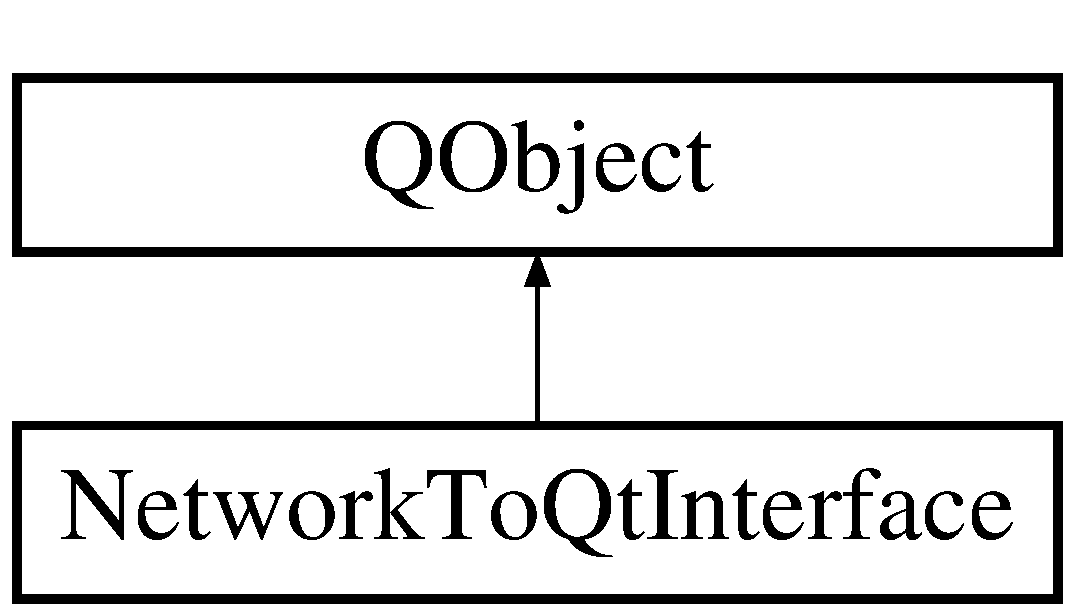
\includegraphics[height=2.000000cm]{classNetworkToQtInterface}
\end{center}
\end{figure}
\subsection*{Public Slots}
\begin{DoxyCompactItemize}
\item 
void \hyperlink{classNetworkToQtInterface_ae998c02ca1c22313b0abc90fc4b7c2a6}{proc\-Request} ()
\begin{DoxyCompactList}\small\item\em Process a request/response sequence. \end{DoxyCompactList}\item 
void \hyperlink{classNetworkToQtInterface_a3413c676b1bb27ddc2df47128cf68c5d}{connection\-Timeout} ()
\begin{DoxyCompactList}\small\item\em Timeout the connection. \end{DoxyCompactList}\item 
void \hyperlink{classNetworkToQtInterface_ac4889eb9f3c5b5e4509252481335200f}{close} ()
\begin{DoxyCompactList}\small\item\em Disconnect from server. \end{DoxyCompactList}\end{DoxyCompactItemize}
\subsection*{Signals}
\begin{DoxyCompactItemize}
\item 
void \hyperlink{classNetworkToQtInterface_aac3748797653d3164ff714edafda229a}{receive\-Finished} ()
\item 
void \hyperlink{classNetworkToQtInterface_a254dd8693e87acd8b05fc36d154b3393}{message\-Dispatch} (Q\-String msg)
\begin{DoxyCompactList}\small\item\em Dispatch a message. \end{DoxyCompactList}\item 
void \hyperlink{classNetworkToQtInterface_a1e20584cc20259fa76c180e087dc1a9f}{finished} ()
\begin{DoxyCompactList}\small\item\em Finish thread execution. \end{DoxyCompactList}\item 
void \hyperlink{classNetworkToQtInterface_a889713b57c1e461e7191add0820bb338}{server\-Disconnected} ()
\begin{DoxyCompactList}\small\item\em Server has disconnected. \end{DoxyCompactList}\end{DoxyCompactItemize}
\subsection*{Public Member Functions}
\begin{DoxyCompactItemize}
\item 
\hyperlink{classNetworkToQtInterface_a35d74d050d8317ad3643f56ca51dd400}{Network\-To\-Qt\-Interface} ()
\begin{DoxyCompactList}\small\item\em Default value constructor. \end{DoxyCompactList}\item 
\hyperlink{classNetworkToQtInterface_aa979e45a30e3fd430b5bc4298aa1831e}{Network\-To\-Qt\-Interface} (\hyperlink{classAddress}{Address} server\-\_\-address)
\begin{DoxyCompactList}\small\item\em Explicit value constructor. \end{DoxyCompactList}\item 
\hyperlink{classNetworkToQtInterface_a1af69a269ee8405c5786696846786e09}{$\sim$\-Network\-To\-Qt\-Interface} ()
\begin{DoxyCompactList}\small\item\em Destructor. \end{DoxyCompactList}\item 
bool \hyperlink{classNetworkToQtInterface_a756963d2d3590e52e5fbef2114066068}{Connect} ()
\begin{DoxyCompactList}\small\item\em Connect to a server. \end{DoxyCompactList}\item 
bool \hyperlink{classNetworkToQtInterface_af61a9805badd3d508f8f9619dc66f82d}{Connect} (\hyperlink{classAddress}{Address} server\-\_\-address)
\begin{DoxyCompactList}\small\item\em Connect to a specific server. \end{DoxyCompactList}\item 
bool \hyperlink{classNetworkToQtInterface_a2584e2afdb435bd83b9bd9bbec6214c3}{is\-Connected} () const 
\begin{DoxyCompactList}\small\item\em Connection status. \end{DoxyCompactList}\item 
void \hyperlink{classNetworkToQtInterface_aed3e3b56739941d40dd8f222f2bfc394}{set\-Buffer} (Q\-String \&data)
\begin{DoxyCompactList}\small\item\em Set the internal message buffer. \end{DoxyCompactList}\item 
void \hyperlink{classNetworkToQtInterface_aa1fc46b9d7bf2e5c219ff36808c555eb}{set\-Server\-Address} (\hyperlink{classAddress}{Address} \&addr)
\begin{DoxyCompactList}\small\item\em Set the server address. \end{DoxyCompactList}\item 
void \hyperlink{classNetworkToQtInterface_a9276c7187edac88dfa06e08f883bc39e}{send\-Message} (const Q\-String \&msg)
\begin{DoxyCompactList}\small\item\em Directly send a message. \end{DoxyCompactList}\end{DoxyCompactItemize}


\subsection{Detailed Description}
The \hyperlink{classNetworkToQtInterface}{Network\-To\-Qt\-Interface} class. 

An interface between Qt and the underlying T\-C\-P client. Objects of this class generally should be moved into another thread before used by connecting a Q\-Thread object's start signal with the \hyperlink{classNetworkToQtInterface_ae998c02ca1c22313b0abc90fc4b7c2a6}{proc\-Request()} slot. 

\subsection{Constructor \& Destructor Documentation}
\hypertarget{classNetworkToQtInterface_a35d74d050d8317ad3643f56ca51dd400}{\index{Network\-To\-Qt\-Interface@{Network\-To\-Qt\-Interface}!Network\-To\-Qt\-Interface@{Network\-To\-Qt\-Interface}}
\index{Network\-To\-Qt\-Interface@{Network\-To\-Qt\-Interface}!NetworkToQtInterface@{Network\-To\-Qt\-Interface}}
\subsubsection[{Network\-To\-Qt\-Interface}]{\setlength{\rightskip}{0pt plus 5cm}Network\-To\-Qt\-Interface\-::\-Network\-To\-Qt\-Interface (
\begin{DoxyParamCaption}
{}
\end{DoxyParamCaption}
)}}\label{classNetworkToQtInterface_a35d74d050d8317ad3643f56ca51dd400}


Default value constructor. 


\begin{DoxyCode}
7                                            :
8     m\_connection\_timeout(\textcolor{keyword}{false}),
9     m\_buffer(\textcolor{stringliteral}{"Buffer"})
10 \{
11 
12 \}
\end{DoxyCode}
\hypertarget{classNetworkToQtInterface_aa979e45a30e3fd430b5bc4298aa1831e}{\index{Network\-To\-Qt\-Interface@{Network\-To\-Qt\-Interface}!Network\-To\-Qt\-Interface@{Network\-To\-Qt\-Interface}}
\index{Network\-To\-Qt\-Interface@{Network\-To\-Qt\-Interface}!NetworkToQtInterface@{Network\-To\-Qt\-Interface}}
\subsubsection[{Network\-To\-Qt\-Interface}]{\setlength{\rightskip}{0pt plus 5cm}Network\-To\-Qt\-Interface\-::\-Network\-To\-Qt\-Interface (
\begin{DoxyParamCaption}
\item[{{\bf Address}}]{server\-\_\-address}
\end{DoxyParamCaption}
)}}\label{classNetworkToQtInterface_aa979e45a30e3fd430b5bc4298aa1831e}


Explicit value constructor. 


\begin{DoxyParams}{Parameters}
{\em server\-\_\-address} & The address to connect to. \\
\hline
\end{DoxyParams}

\begin{DoxyCode}
14                                                                  :
15     m\_server\_address(server\_address),
16     m\_connection\_timeout(\textcolor{keyword}{false}),
17     m\_buffer(\textcolor{stringliteral}{"Buffer"})
18 \{
19 
20 \}
\end{DoxyCode}
\hypertarget{classNetworkToQtInterface_a1af69a269ee8405c5786696846786e09}{\index{Network\-To\-Qt\-Interface@{Network\-To\-Qt\-Interface}!$\sim$\-Network\-To\-Qt\-Interface@{$\sim$\-Network\-To\-Qt\-Interface}}
\index{$\sim$\-Network\-To\-Qt\-Interface@{$\sim$\-Network\-To\-Qt\-Interface}!NetworkToQtInterface@{Network\-To\-Qt\-Interface}}
\subsubsection[{$\sim$\-Network\-To\-Qt\-Interface}]{\setlength{\rightskip}{0pt plus 5cm}Network\-To\-Qt\-Interface\-::$\sim$\-Network\-To\-Qt\-Interface (
\begin{DoxyParamCaption}
{}
\end{DoxyParamCaption}
)}}\label{classNetworkToQtInterface_a1af69a269ee8405c5786696846786e09}


Destructor. 


\begin{DoxyCode}
23 \{
24     \textcolor{comment}{//Delete members}
25     \textcolor{comment}{//delete m\_response\_loop;}
26 \}
\end{DoxyCode}


\subsection{Member Function Documentation}
\hypertarget{classNetworkToQtInterface_ac4889eb9f3c5b5e4509252481335200f}{\index{Network\-To\-Qt\-Interface@{Network\-To\-Qt\-Interface}!close@{close}}
\index{close@{close}!NetworkToQtInterface@{Network\-To\-Qt\-Interface}}
\subsubsection[{close}]{\setlength{\rightskip}{0pt plus 5cm}void Network\-To\-Qt\-Interface\-::close (
\begin{DoxyParamCaption}
{}
\end{DoxyParamCaption}
)\hspace{0.3cm}{\ttfamily [slot]}}}\label{classNetworkToQtInterface_ac4889eb9f3c5b5e4509252481335200f}


Disconnect from server. 

Slot which will disconnect from the server. 
\begin{DoxyCode}
56 \{
57     \textcolor{comment}{//Close the connection}
58     m\_tcp\_client.\hyperlink{classTCPClient_aeef43b15ef57aefead37ff7300ebc779}{disconnect}();
59     \textcolor{comment}{//emit messageDispatch("Disconnected from server!");}
60 \}
\end{DoxyCode}
\hypertarget{classNetworkToQtInterface_a756963d2d3590e52e5fbef2114066068}{\index{Network\-To\-Qt\-Interface@{Network\-To\-Qt\-Interface}!Connect@{Connect}}
\index{Connect@{Connect}!NetworkToQtInterface@{Network\-To\-Qt\-Interface}}
\subsubsection[{Connect}]{\setlength{\rightskip}{0pt plus 5cm}bool Network\-To\-Qt\-Interface\-::\-Connect (
\begin{DoxyParamCaption}
{}
\end{DoxyParamCaption}
)}}\label{classNetworkToQtInterface_a756963d2d3590e52e5fbef2114066068}


Connect to a server. 

Connect to the server whose address is represented by the field m\-\_\-server\-\_\-address. \begin{DoxyReturn}{Returns}
True if connection succeeded, false otherwise. 
\end{DoxyReturn}

\begin{DoxyCode}
37 \{
38     \textcolor{comment}{//m\_connection\_timeout = false;}
39     \textcolor{comment}{//Start a one shot timer to timeout after 10 seconds}
40    \textcolor{comment}{// QTimer::singleShot(1000, this, SLOT(connectionTimeout()));}
41     \textcolor{comment}{//Attempt to connect}
42     \hyperlink{tcpclient_8h_ab36b81f0daebbad95a533ea9951ee569}{TCPError} connected = m\_tcp\_client.\hyperlink{classTCPClient_adb1706d816b7810d28ef9eeab77a423b}{connectToServer}(m\_server\_address);
43 
44 \textcolor{comment}{//    if(connected == TCP\_STATUS\_SUCCESS)}
45 \textcolor{comment}{//    \{}
46 \textcolor{comment}{//        emit messageDispatch("Connected!");}
47 \textcolor{comment}{//    \}}
48 \textcolor{comment}{//    else}
49 \textcolor{comment}{//    \{}
50 \textcolor{comment}{//        emit messageDispatch("Unable to connect!");}
51 \textcolor{comment}{//    \}}
52     \textcolor{keywordflow}{return} connected == \hyperlink{tcpclient_8h_ab36b81f0daebbad95a533ea9951ee569a12de2815c3e64df634ac4d26a0bb2007}{TCP\_STATUS\_SUCCESS};
53 \}
\end{DoxyCode}
\hypertarget{classNetworkToQtInterface_af61a9805badd3d508f8f9619dc66f82d}{\index{Network\-To\-Qt\-Interface@{Network\-To\-Qt\-Interface}!Connect@{Connect}}
\index{Connect@{Connect}!NetworkToQtInterface@{Network\-To\-Qt\-Interface}}
\subsubsection[{Connect}]{\setlength{\rightskip}{0pt plus 5cm}bool Network\-To\-Qt\-Interface\-::\-Connect (
\begin{DoxyParamCaption}
\item[{{\bf Address}}]{server\-\_\-address}
\end{DoxyParamCaption}
)}}\label{classNetworkToQtInterface_af61a9805badd3d508f8f9619dc66f82d}


Connect to a specific server. 

Connect to the server represented by the parameter server\-\_\-address. 
\begin{DoxyParams}{Parameters}
{\em server\-\_\-address} & The address to connect to. \\
\hline
\end{DoxyParams}
\begin{DoxyReturn}{Returns}
True if connection succeeded, false otherwise. 
\end{DoxyReturn}
\hypertarget{classNetworkToQtInterface_a3413c676b1bb27ddc2df47128cf68c5d}{\index{Network\-To\-Qt\-Interface@{Network\-To\-Qt\-Interface}!connection\-Timeout@{connection\-Timeout}}
\index{connection\-Timeout@{connection\-Timeout}!NetworkToQtInterface@{Network\-To\-Qt\-Interface}}
\subsubsection[{connection\-Timeout}]{\setlength{\rightskip}{0pt plus 5cm}void Network\-To\-Qt\-Interface\-::connection\-Timeout (
\begin{DoxyParamCaption}
{}
\end{DoxyParamCaption}
)\hspace{0.3cm}{\ttfamily [slot]}}}\label{classNetworkToQtInterface_a3413c676b1bb27ddc2df47128cf68c5d}


Timeout the connection. 

Slot which will set an internal flag indicating that the connection has timed out. 
\begin{DoxyCode}
79 \{
80     m\_connection\_timeout = \textcolor{keyword}{true};
81 \}
\end{DoxyCode}
\hypertarget{classNetworkToQtInterface_a1e20584cc20259fa76c180e087dc1a9f}{\index{Network\-To\-Qt\-Interface@{Network\-To\-Qt\-Interface}!finished@{finished}}
\index{finished@{finished}!NetworkToQtInterface@{Network\-To\-Qt\-Interface}}
\subsubsection[{finished}]{\setlength{\rightskip}{0pt plus 5cm}void Network\-To\-Qt\-Interface\-::finished (
\begin{DoxyParamCaption}
{}
\end{DoxyParamCaption}
)\hspace{0.3cm}{\ttfamily [signal]}}}\label{classNetworkToQtInterface_a1e20584cc20259fa76c180e087dc1a9f}


Finish thread execution. 

Signal to indicate end of execution of the \hyperlink{classNetworkToQtInterface_ae998c02ca1c22313b0abc90fc4b7c2a6}{proc\-Request()} sequence. \hypertarget{classNetworkToQtInterface_a2584e2afdb435bd83b9bd9bbec6214c3}{\index{Network\-To\-Qt\-Interface@{Network\-To\-Qt\-Interface}!is\-Connected@{is\-Connected}}
\index{is\-Connected@{is\-Connected}!NetworkToQtInterface@{Network\-To\-Qt\-Interface}}
\subsubsection[{is\-Connected}]{\setlength{\rightskip}{0pt plus 5cm}bool Network\-To\-Qt\-Interface\-::is\-Connected (
\begin{DoxyParamCaption}
{}
\end{DoxyParamCaption}
) const}}\label{classNetworkToQtInterface_a2584e2afdb435bd83b9bd9bbec6214c3}


Connection status. 

Indicate whether or not this object is connected to a server. \begin{DoxyReturn}{Returns}
True if connected to a server, false otherwise. 
\end{DoxyReturn}

\begin{DoxyCode}
127 \{
128     \textcolor{keywordflow}{return} m\_tcp\_client.\hyperlink{classTCPClient_a30054a07061dfe22e7a9a7783a843bcc}{isConnected}();
129 \}
\end{DoxyCode}
\hypertarget{classNetworkToQtInterface_a254dd8693e87acd8b05fc36d154b3393}{\index{Network\-To\-Qt\-Interface@{Network\-To\-Qt\-Interface}!message\-Dispatch@{message\-Dispatch}}
\index{message\-Dispatch@{message\-Dispatch}!NetworkToQtInterface@{Network\-To\-Qt\-Interface}}
\subsubsection[{message\-Dispatch}]{\setlength{\rightskip}{0pt plus 5cm}void Network\-To\-Qt\-Interface\-::message\-Dispatch (
\begin{DoxyParamCaption}
\item[{Q\-String}]{msg}
\end{DoxyParamCaption}
)\hspace{0.3cm}{\ttfamily [signal]}}}\label{classNetworkToQtInterface_a254dd8693e87acd8b05fc36d154b3393}


Dispatch a message. 

Signal that is emitted when an event occurs in the \hyperlink{classNetworkToQtInterface_ae998c02ca1c22313b0abc90fc4b7c2a6}{proc\-Request()} sequence that will send a message containing information about the current state of execution (i.\-e. server response, error messages) 
\begin{DoxyParams}{Parameters}
{\em msg} & The message to send to connected handlers. \\
\hline
\end{DoxyParams}
\hypertarget{classNetworkToQtInterface_ae998c02ca1c22313b0abc90fc4b7c2a6}{\index{Network\-To\-Qt\-Interface@{Network\-To\-Qt\-Interface}!proc\-Request@{proc\-Request}}
\index{proc\-Request@{proc\-Request}!NetworkToQtInterface@{Network\-To\-Qt\-Interface}}
\subsubsection[{proc\-Request}]{\setlength{\rightskip}{0pt plus 5cm}void Network\-To\-Qt\-Interface\-::proc\-Request (
\begin{DoxyParamCaption}
{}
\end{DoxyParamCaption}
)\hspace{0.3cm}{\ttfamily [slot]}}}\label{classNetworkToQtInterface_ae998c02ca1c22313b0abc90fc4b7c2a6}


Process a request/response sequence. 

A slot which will begin a request response sequence; A message is attempted to be sent to the server. If successful, this function will wait until the server responds, and will emit a message\-Dispatch signal with either the server's response or an error message. 
\begin{DoxyCode}
63 \{
64     \hyperlink{tcpclient_8h_ab36b81f0daebbad95a533ea9951ee569}{TCPError} status = \hyperlink{tcpclient_8h_ab36b81f0daebbad95a533ea9951ee569a12de2815c3e64df634ac4d26a0bb2007}{TCP\_STATUS\_SUCCESS};
65     \textcolor{comment}{//First, send the request}
66     m\_buffer.append(\textcolor{charliteral}{'\(\backslash\)n'});
67     \textcolor{keyword}{const} \textcolor{keywordtype}{char} *data = m\_buffer.toStdString().c\_str();
68     \textcolor{comment}{//INFO() << "Just before send... Data:" << data;}
69     status = m\_tcp\_client.\hyperlink{classTCPClient_a23a640eac58e631288cdeb479416e0ed}{Send}(data, strlen(data));
70     \hyperlink{Log_8h_a7cec51f4ce4b22e8c0f256485d57fca7}{INFO}() << \textcolor{stringliteral}{"After send. STATUS: "} << status;
71     \textcolor{comment}{//Handle error}
72     \textcolor{comment}{//check for a request for 5 seconds}
73     \textcolor{comment}{//Set up timer}
74     this->setUpTimer();
75     this->m\_response\_loop->\hyperlink{classTickingTimer_a0f7c3da243271bcd1ffa833ebdc9c3a4}{startTicking}(500);
76 \}
\end{DoxyCode}
\hypertarget{classNetworkToQtInterface_aac3748797653d3164ff714edafda229a}{\index{Network\-To\-Qt\-Interface@{Network\-To\-Qt\-Interface}!receive\-Finished@{receive\-Finished}}
\index{receive\-Finished@{receive\-Finished}!NetworkToQtInterface@{Network\-To\-Qt\-Interface}}
\subsubsection[{receive\-Finished}]{\setlength{\rightskip}{0pt plus 5cm}void Network\-To\-Qt\-Interface\-::receive\-Finished (
\begin{DoxyParamCaption}
{}
\end{DoxyParamCaption}
)\hspace{0.3cm}{\ttfamily [signal]}}}\label{classNetworkToQtInterface_aac3748797653d3164ff714edafda229a}
\hypertarget{classNetworkToQtInterface_a9276c7187edac88dfa06e08f883bc39e}{\index{Network\-To\-Qt\-Interface@{Network\-To\-Qt\-Interface}!send\-Message@{send\-Message}}
\index{send\-Message@{send\-Message}!NetworkToQtInterface@{Network\-To\-Qt\-Interface}}
\subsubsection[{send\-Message}]{\setlength{\rightskip}{0pt plus 5cm}void Network\-To\-Qt\-Interface\-::send\-Message (
\begin{DoxyParamCaption}
\item[{const Q\-String \&}]{msg}
\end{DoxyParamCaption}
)}}\label{classNetworkToQtInterface_a9276c7187edac88dfa06e08f883bc39e}


Directly send a message. 

Immediately send the message msg to the server this object is connected to, or send nothing if not connected to a server. 
\begin{DoxyParams}{Parameters}
{\em msg} & The message to send \\
\hline
\end{DoxyParams}

\begin{DoxyCode}
142 \{
143     \textcolor{keywordflow}{if}(m\_tcp\_client.\hyperlink{classTCPClient_a30054a07061dfe22e7a9a7783a843bcc}{isConnected}())
144         m\_tcp\_client.\hyperlink{classTCPClient_a23a640eac58e631288cdeb479416e0ed}{Send}(msg.toStdString().c\_str(), msg.size());
145 \}
\end{DoxyCode}
\hypertarget{classNetworkToQtInterface_a889713b57c1e461e7191add0820bb338}{\index{Network\-To\-Qt\-Interface@{Network\-To\-Qt\-Interface}!server\-Disconnected@{server\-Disconnected}}
\index{server\-Disconnected@{server\-Disconnected}!NetworkToQtInterface@{Network\-To\-Qt\-Interface}}
\subsubsection[{server\-Disconnected}]{\setlength{\rightskip}{0pt plus 5cm}void Network\-To\-Qt\-Interface\-::server\-Disconnected (
\begin{DoxyParamCaption}
{}
\end{DoxyParamCaption}
)\hspace{0.3cm}{\ttfamily [signal]}}}\label{classNetworkToQtInterface_a889713b57c1e461e7191add0820bb338}


Server has disconnected. 

Signal to indicate that the server has disconnected. \hypertarget{classNetworkToQtInterface_aed3e3b56739941d40dd8f222f2bfc394}{\index{Network\-To\-Qt\-Interface@{Network\-To\-Qt\-Interface}!set\-Buffer@{set\-Buffer}}
\index{set\-Buffer@{set\-Buffer}!NetworkToQtInterface@{Network\-To\-Qt\-Interface}}
\subsubsection[{set\-Buffer}]{\setlength{\rightskip}{0pt plus 5cm}void Network\-To\-Qt\-Interface\-::set\-Buffer (
\begin{DoxyParamCaption}
\item[{Q\-String \&}]{data}
\end{DoxyParamCaption}
)}}\label{classNetworkToQtInterface_aed3e3b56739941d40dd8f222f2bfc394}


Set the internal message buffer. 

Set the internal buffer containing the message to be sent to the server. This internal buffer is used when the \hyperlink{classNetworkToQtInterface_ae998c02ca1c22313b0abc90fc4b7c2a6}{proc\-Request()} slot is invoked, generally when the thread that an object of \hyperlink{classNetworkToQtInterface}{Network\-To\-Qt\-Interface} type is moved to issues it's start signal. 
\begin{DoxyParams}{Parameters}
{\em data} & The message to send to the server. \\
\hline
\end{DoxyParams}

\begin{DoxyCode}
132 \{
133     m\_buffer = data;
134 \}
\end{DoxyCode}
\hypertarget{classNetworkToQtInterface_aa1fc46b9d7bf2e5c219ff36808c555eb}{\index{Network\-To\-Qt\-Interface@{Network\-To\-Qt\-Interface}!set\-Server\-Address@{set\-Server\-Address}}
\index{set\-Server\-Address@{set\-Server\-Address}!NetworkToQtInterface@{Network\-To\-Qt\-Interface}}
\subsubsection[{set\-Server\-Address}]{\setlength{\rightskip}{0pt plus 5cm}void Network\-To\-Qt\-Interface\-::set\-Server\-Address (
\begin{DoxyParamCaption}
\item[{{\bf Address} \&}]{addr}
\end{DoxyParamCaption}
)}}\label{classNetworkToQtInterface_aa1fc46b9d7bf2e5c219ff36808c555eb}


Set the server address. 

Set the server address that this object should connect to when the \hyperlink{classNetworkToQtInterface_a756963d2d3590e52e5fbef2114066068}{Connect()} call is made. 
\begin{DoxyParams}{Parameters}
{\em addr} & The address to set. \\
\hline
\end{DoxyParams}

\begin{DoxyCode}
137 \{
138     this->m\_server\_address = addr;
139 \}
\end{DoxyCode}


The documentation for this class was generated from the following files\-:\begin{DoxyCompactItemize}
\item 
Network/\hyperlink{networktoqtinterface_8h}{networktoqtinterface.\-h}\item 
Network/\hyperlink{networktoqtinterface_8cpp}{networktoqtinterface.\-cpp}\end{DoxyCompactItemize}

\hypertarget{structnot__equal__to}{\section{not\-\_\-equal\-\_\-to Struct Reference}
\label{structnot__equal__to}\index{not\-\_\-equal\-\_\-to@{not\-\_\-equal\-\_\-to}}
}
\subsection*{Public Member Functions}
\begin{DoxyCompactItemize}
\item 
{\footnotesize template$<$typename T $>$ }\\bool \hyperlink{structnot__equal__to_acbcb7d0809378458b52e6ed1a07c1d7d}{operator()} (const T \&lhs, const T \&rhs) const 
\end{DoxyCompactItemize}


\subsection{Member Function Documentation}
\hypertarget{structnot__equal__to_acbcb7d0809378458b52e6ed1a07c1d7d}{\index{not\-\_\-equal\-\_\-to@{not\-\_\-equal\-\_\-to}!operator()@{operator()}}
\index{operator()@{operator()}!not_equal_to@{not\-\_\-equal\-\_\-to}}
\subsubsection[{operator()}]{\setlength{\rightskip}{0pt plus 5cm}template$<$typename T $>$ bool not\-\_\-equal\-\_\-to\-::operator() (
\begin{DoxyParamCaption}
\item[{const T \&}]{lhs, }
\item[{const T \&}]{rhs}
\end{DoxyParamCaption}
) const\hspace{0.3cm}{\ttfamily [inline]}}}\label{structnot__equal__to_acbcb7d0809378458b52e6ed1a07c1d7d}

\begin{DoxyCode}
5436         \{
5437             \textcolor{keywordflow}{return} lhs != rhs;
5438         \}
\end{DoxyCode}


The documentation for this struct was generated from the following file\-:\begin{DoxyCompactItemize}
\item 
Third\-Party/pugixml/\hyperlink{pugixml_8cpp}{pugixml.\-cpp}\end{DoxyCompactItemize}

\hypertarget{structopt__false}{\section{opt\-\_\-false Struct Reference}
\label{structopt__false}\index{opt\-\_\-false@{opt\-\_\-false}}
}
\subsection*{Public Types}
\begin{DoxyCompactItemize}
\item 
enum \{ \hyperlink{structopt__false_adf1eb3ad7c3e284bd861d80d6817174fa0608b30b4b0f63ec3263f29fe847899e}{value} = 0
 \}
\end{DoxyCompactItemize}


\subsection{Member Enumeration Documentation}
\hypertarget{structopt__false_adf1eb3ad7c3e284bd861d80d6817174f}{\subsubsection[{anonymous enum}]{\setlength{\rightskip}{0pt plus 5cm}anonymous enum}}\label{structopt__false_adf1eb3ad7c3e284bd861d80d6817174f}
\begin{Desc}
\item[Enumerator]\par
\begin{description}
\index{value@{value}!opt\-\_\-false@{opt\-\_\-false}}\index{opt\-\_\-false@{opt\-\_\-false}!value@{value}}\item[{\em 
\hypertarget{structopt__false_adf1eb3ad7c3e284bd861d80d6817174fa0608b30b4b0f63ec3263f29fe847899e}{value}\label{structopt__false_adf1eb3ad7c3e284bd861d80d6817174fa0608b30b4b0f63ec3263f29fe847899e}
}]\end{description}
\end{Desc}

\begin{DoxyCode}
634 \{ \hyperlink{structopt__false_adf1eb3ad7c3e284bd861d80d6817174fa0608b30b4b0f63ec3263f29fe847899e}{value} = 0 \};
\end{DoxyCode}


The documentation for this struct was generated from the following file\-:\begin{DoxyCompactItemize}
\item 
Third\-Party/pugixml/\hyperlink{pugixml_8cpp}{pugixml.\-cpp}\end{DoxyCompactItemize}

\hypertarget{structopt__true}{\section{opt\-\_\-true Struct Reference}
\label{structopt__true}\index{opt\-\_\-true@{opt\-\_\-true}}
}
\subsection*{Public Types}
\begin{DoxyCompactItemize}
\item 
enum \{ \hyperlink{structopt__true_a93a7039f202aca3a935c98aa8e069ea5a3f8405655cc98a5710236f177e042b72}{value} = 1
 \}
\end{DoxyCompactItemize}


\subsection{Member Enumeration Documentation}
\hypertarget{structopt__true_a93a7039f202aca3a935c98aa8e069ea5}{\subsubsection[{anonymous enum}]{\setlength{\rightskip}{0pt plus 5cm}anonymous enum}}\label{structopt__true_a93a7039f202aca3a935c98aa8e069ea5}
\begin{Desc}
\item[Enumerator]\par
\begin{description}
\index{value@{value}!opt\-\_\-true@{opt\-\_\-true}}\index{opt\-\_\-true@{opt\-\_\-true}!value@{value}}\item[{\em 
\hypertarget{structopt__true_a93a7039f202aca3a935c98aa8e069ea5a3f8405655cc98a5710236f177e042b72}{value}\label{structopt__true_a93a7039f202aca3a935c98aa8e069ea5a3f8405655cc98a5710236f177e042b72}
}]\end{description}
\end{Desc}

\begin{DoxyCode}
639 \{ \hyperlink{structopt__true_a93a7039f202aca3a935c98aa8e069ea5a3f8405655cc98a5710236f177e042b72}{value} = 1 \};
\end{DoxyCode}


The documentation for this struct was generated from the following file\-:\begin{DoxyCompactItemize}
\item 
Third\-Party/pugixml/\hyperlink{pugixml_8cpp}{pugixml.\-cpp}\end{DoxyCompactItemize}

\hypertarget{classPacketReceiver}{\section{Packet\-Receiver Class Reference}
\label{classPacketReceiver}\index{Packet\-Receiver@{Packet\-Receiver}}
}


{\ttfamily \#include $<$packetreceiver.\-h$>$}

Inheritance diagram for Packet\-Receiver\-:\begin{figure}[H]
\begin{center}
\leavevmode
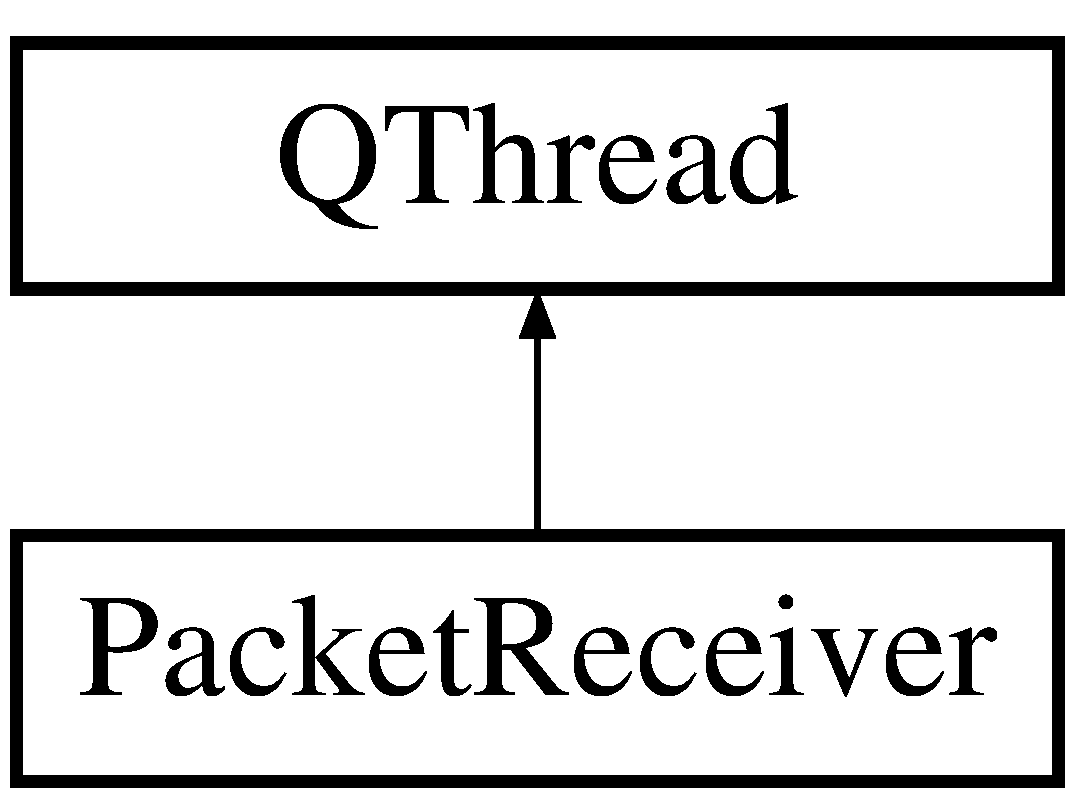
\includegraphics[height=2.000000cm]{classPacketReceiver}
\end{center}
\end{figure}
\subsection*{Public Member Functions}
\begin{DoxyCompactItemize}
\item 
\hyperlink{classPacketReceiver_a336af20ed7b74dfd8ce5603ba89fc8c3}{Packet\-Receiver} (\hyperlink{classMessageDispatcher}{Message\-Dispatcher} $\ast$passer)
\item 
\hyperlink{classPacketReceiver_aaa7c59a15a919bb7842ed062199876cf}{$\sim$\-Packet\-Receiver} ()
\item 
void \hyperlink{classPacketReceiver_ad290dd22371f82675ee530fd123399a4}{wait\-To\-Finish} ()
\end{DoxyCompactItemize}
\subsection*{Protected Member Functions}
\begin{DoxyCompactItemize}
\item 
void \hyperlink{classPacketReceiver_abb2ff260250bf7baf8303f4ae1e1aa7e}{run} ()
\end{DoxyCompactItemize}


\subsection{Constructor \& Destructor Documentation}
\hypertarget{classPacketReceiver_a336af20ed7b74dfd8ce5603ba89fc8c3}{\index{Packet\-Receiver@{Packet\-Receiver}!Packet\-Receiver@{Packet\-Receiver}}
\index{Packet\-Receiver@{Packet\-Receiver}!PacketReceiver@{Packet\-Receiver}}
\subsubsection[{Packet\-Receiver}]{\setlength{\rightskip}{0pt plus 5cm}Packet\-Receiver\-::\-Packet\-Receiver (
\begin{DoxyParamCaption}
\item[{{\bf Message\-Dispatcher} $\ast$}]{passer}
\end{DoxyParamCaption}
)}}\label{classPacketReceiver_a336af20ed7b74dfd8ce5603ba89fc8c3}

\begin{DoxyCode}
8                                                          :
9     m\_dispatcher(passer),
10     valid(\textcolor{keyword}{true}),
11     finishing(\textcolor{keyword}{false})
12 \{
13 \}
\end{DoxyCode}
\hypertarget{classPacketReceiver_aaa7c59a15a919bb7842ed062199876cf}{\index{Packet\-Receiver@{Packet\-Receiver}!$\sim$\-Packet\-Receiver@{$\sim$\-Packet\-Receiver}}
\index{$\sim$\-Packet\-Receiver@{$\sim$\-Packet\-Receiver}!PacketReceiver@{Packet\-Receiver}}
\subsubsection[{$\sim$\-Packet\-Receiver}]{\setlength{\rightskip}{0pt plus 5cm}Packet\-Receiver\-::$\sim$\-Packet\-Receiver (
\begin{DoxyParamCaption}
{}
\end{DoxyParamCaption}
)}}\label{classPacketReceiver_aaa7c59a15a919bb7842ed062199876cf}

\begin{DoxyCode}
16 \{
17     \textcolor{keyword}{delete} data;
18 \}
\end{DoxyCode}


\subsection{Member Function Documentation}
\hypertarget{classPacketReceiver_abb2ff260250bf7baf8303f4ae1e1aa7e}{\index{Packet\-Receiver@{Packet\-Receiver}!run@{run}}
\index{run@{run}!PacketReceiver@{Packet\-Receiver}}
\subsubsection[{run}]{\setlength{\rightskip}{0pt plus 5cm}void Packet\-Receiver\-::run (
\begin{DoxyParamCaption}
{}
\end{DoxyParamCaption}
)\hspace{0.3cm}{\ttfamily [protected]}}}\label{classPacketReceiver_abb2ff260250bf7baf8303f4ae1e1aa7e}

\begin{DoxyCode}
31 \{
32     \hyperlink{classSocket}{Socket} sock;
33     \textcolor{keywordtype}{bool} status = sock.\hyperlink{classSocket_a7d7e4c8274e8028cc56f5778f98936b1}{Open}((\textcolor{keywordtype}{unsigned} \textcolor{keywordtype}{short}) \hyperlink{SocketConstants_8h_a4fba0963c20988d1f1a45afb1c636e44}{LISTEN\_PORT});
34     \textcolor{comment}{//Delegate string to dispatch to main window}
35     std::string message\_delegate;
36     \textcolor{keywordflow}{if}(status)
37     \{
38         data = \textcolor{keyword}{new} \textcolor{keywordtype}{char}[256];
39         \hyperlink{classAddress}{Address} fromAddress;
40         \hyperlink{Log_8h_a7cec51f4ce4b22e8c0f256485d57fca7}{INFO}() << \textcolor{stringliteral}{"Beginning packet reception loop"};
41         \textcolor{keywordtype}{bool} received = \textcolor{keyword}{false};
42         \textcolor{comment}{//Begin loop to receive packet}
43         \textcolor{keywordflow}{while}(valid)
44         \{
45             \textcolor{keywordflow}{if}(data == NULL)
46                 data = \textcolor{keyword}{new} \textcolor{keywordtype}{char}[256];
47            received = sock.\hyperlink{classSocket_a24d0d17efdaab291e81d5d89b463a585}{Receive}(fromAddress, (\textcolor{keywordtype}{void} *)data, strlen(data));
48 
49             \textcolor{keywordflow}{if}(received)
50             \{
51                 \hyperlink{Log_8h_a7cec51f4ce4b22e8c0f256485d57fca7}{INFO}() << \textcolor{stringliteral}{"Received packet, emitting signal. Payload:"} << data;
52                 \textcolor{comment}{//Give the data to a delegate so we can delete the pointer}
53                 message\_delegate.assign(data, strlen((\textcolor{keyword}{const} \textcolor{keywordtype}{char} *)data));
54                 this->m\_dispatcher->\hyperlink{classMessageDispatcher_a5c3f81bf5d598bb5f3833ef0d6e140a7}{reemitMessage}(message\_delegate.data());
55                 \hyperlink{Log_8h_a7cec51f4ce4b22e8c0f256485d57fca7}{INFO}() << \textcolor{stringliteral}{"After signal emit"};
56                 \textcolor{comment}{//Delete data and set to null}
57                 \textcolor{keyword}{delete} data;
58                 data = NULL;
59             \}
60         \}
61         finishing = \textcolor{keyword}{false};
62 
63     \}
64 \}
\end{DoxyCode}
\hypertarget{classPacketReceiver_ad290dd22371f82675ee530fd123399a4}{\index{Packet\-Receiver@{Packet\-Receiver}!wait\-To\-Finish@{wait\-To\-Finish}}
\index{wait\-To\-Finish@{wait\-To\-Finish}!PacketReceiver@{Packet\-Receiver}}
\subsubsection[{wait\-To\-Finish}]{\setlength{\rightskip}{0pt plus 5cm}void Packet\-Receiver\-::wait\-To\-Finish (
\begin{DoxyParamCaption}
{}
\end{DoxyParamCaption}
)}}\label{classPacketReceiver_ad290dd22371f82675ee530fd123399a4}

\begin{DoxyCode}
21 \{
22     \textcolor{comment}{//Finish this thread}
23     finishing = \textcolor{keyword}{true};
24     \textcolor{keywordflow}{while}(finishing)
25     \{
26         this->valid = \textcolor{keyword}{false};
27     \}
28 \}
\end{DoxyCode}


The documentation for this class was generated from the following files\-:\begin{DoxyCompactItemize}
\item 
Util/\hyperlink{packetreceiver_8h}{packetreceiver.\-h}\item 
Util/\hyperlink{packetreceiver_8cpp}{packetreceiver.\-cpp}\end{DoxyCompactItemize}

\hypertarget{classPacketSender}{\section{Packet\-Sender Class Reference}
\label{classPacketSender}\index{Packet\-Sender@{Packet\-Sender}}
}


{\ttfamily \#include $<$packetsender.\-h$>$}

Inheritance diagram for Packet\-Sender\-:\begin{figure}[H]
\begin{center}
\leavevmode
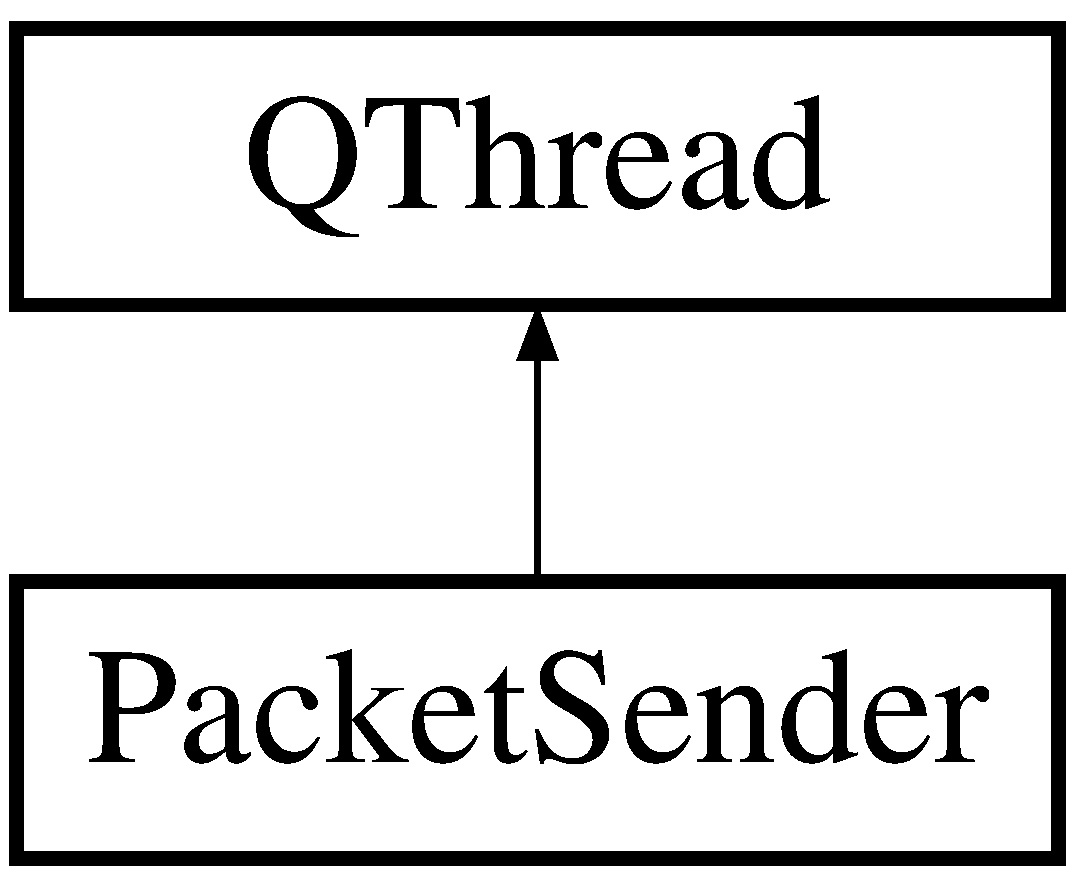
\includegraphics[height=2.000000cm]{classPacketSender}
\end{center}
\end{figure}
\subsection*{Public Member Functions}
\begin{DoxyCompactItemize}
\item 
\hyperlink{classPacketSender_a7d1fdff7ead38f3a32149facf14fe5fc}{Packet\-Sender} ()
\item 
char $\ast$ \hyperlink{classPacketSender_adf62a2c7ff2bbac54990764630705ce5}{get\-Buffer} () const 
\item 
void \hyperlink{classPacketSender_a987e41bbb8e8423af5d9e25f7ddcf3e0}{set\-Buffer} (const char $\ast$buffer)
\end{DoxyCompactItemize}
\subsection*{Protected Member Functions}
\begin{DoxyCompactItemize}
\item 
void \hyperlink{classPacketSender_adac7fe40c40a0a32a1a95f431acad704}{run} ()
\end{DoxyCompactItemize}


\subsection{Constructor \& Destructor Documentation}
\hypertarget{classPacketSender_a7d1fdff7ead38f3a32149facf14fe5fc}{\index{Packet\-Sender@{Packet\-Sender}!Packet\-Sender@{Packet\-Sender}}
\index{Packet\-Sender@{Packet\-Sender}!PacketSender@{Packet\-Sender}}
\subsubsection[{Packet\-Sender}]{\setlength{\rightskip}{0pt plus 5cm}Packet\-Sender\-::\-Packet\-Sender (
\begin{DoxyParamCaption}
{}
\end{DoxyParamCaption}
)}}\label{classPacketSender_a7d1fdff7ead38f3a32149facf14fe5fc}

\begin{DoxyCode}
10 \{
11 \}
\end{DoxyCode}


\subsection{Member Function Documentation}
\hypertarget{classPacketSender_adf62a2c7ff2bbac54990764630705ce5}{\index{Packet\-Sender@{Packet\-Sender}!get\-Buffer@{get\-Buffer}}
\index{get\-Buffer@{get\-Buffer}!PacketSender@{Packet\-Sender}}
\subsubsection[{get\-Buffer}]{\setlength{\rightskip}{0pt plus 5cm}char $\ast$ Packet\-Sender\-::get\-Buffer (
\begin{DoxyParamCaption}
{}
\end{DoxyParamCaption}
) const}}\label{classPacketSender_adf62a2c7ff2bbac54990764630705ce5}

\begin{DoxyCode}
38 \{
39     \textcolor{keywordflow}{return} this->m\_buffer;
40 \}
\end{DoxyCode}
\hypertarget{classPacketSender_adac7fe40c40a0a32a1a95f431acad704}{\index{Packet\-Sender@{Packet\-Sender}!run@{run}}
\index{run@{run}!PacketSender@{Packet\-Sender}}
\subsubsection[{run}]{\setlength{\rightskip}{0pt plus 5cm}void Packet\-Sender\-::run (
\begin{DoxyParamCaption}
{}
\end{DoxyParamCaption}
)\hspace{0.3cm}{\ttfamily [protected]}}}\label{classPacketSender_adac7fe40c40a0a32a1a95f431acad704}

\begin{DoxyCode}
14 \{
15     \hyperlink{classSocket}{Socket} sock;
16     \textcolor{comment}{//Lock this process}
17     this->m\_mutex.lock();
18     \textcolor{keywordtype}{bool} status = sock.\hyperlink{classSocket_a7d7e4c8274e8028cc56f5778f98936b1}{Open}((\textcolor{keywordtype}{unsigned} \textcolor{keywordtype}{short}) \hyperlink{SocketConstants_8h_a92df38b61b193ac6bf60131babe08614}{SEND\_PORT});
19     \textcolor{keywordflow}{if}(status)
20     \{
21         \hyperlink{Log_8h_a7cec51f4ce4b22e8c0f256485d57fca7}{INFO}() << \textcolor{stringliteral}{"Setting up receiver address.........."};
22         \hyperlink{classAddress}{Address} addr(\hyperlink{SocketConstants_8h_abcacfe0cacacfd5ec6a24b96e49715c3}{RECEIVER\_ADDRESS}, \hyperlink{SocketConstants_8h_a714d0c166e470fe1d95e17305a084931}{RECEIVER\_PORT});
23         \hyperlink{Log_8h_a7cec51f4ce4b22e8c0f256485d57fca7}{INFO}() << \textcolor{stringliteral}{"Send data: "} << this->m\_buffer;
24         status = sock.\hyperlink{classSocket_a58639d5ede0d7f4ddd8b96ac8c6c0b9b}{Send}(addr, this->m\_buffer, strlen(this->m\_buffer));
25 
26     \}
27     \textcolor{keywordflow}{else}
28     \{
29         \hyperlink{Log_8h_a1a242c34c5066fb0c62d909f22d3716d}{L\_ERROR}() << \textcolor{stringliteral}{"UNABLE TO OPEN SOCKET......."};
30     \}
31     \textcolor{comment}{//Unlock process}
32     this->m\_mutex.unlock();
33 \}
\end{DoxyCode}
\hypertarget{classPacketSender_a987e41bbb8e8423af5d9e25f7ddcf3e0}{\index{Packet\-Sender@{Packet\-Sender}!set\-Buffer@{set\-Buffer}}
\index{set\-Buffer@{set\-Buffer}!PacketSender@{Packet\-Sender}}
\subsubsection[{set\-Buffer}]{\setlength{\rightskip}{0pt plus 5cm}void Packet\-Sender\-::set\-Buffer (
\begin{DoxyParamCaption}
\item[{const char $\ast$}]{buffer}
\end{DoxyParamCaption}
)}}\label{classPacketSender_a987e41bbb8e8423af5d9e25f7ddcf3e0}

\begin{DoxyCode}
44 \{
45     this->m\_buffer = (\textcolor{keywordtype}{char} *)buffer;
46 \}
\end{DoxyCode}


The documentation for this class was generated from the following files\-:\begin{DoxyCompactItemize}
\item 
Util/\hyperlink{packetsender_8h}{packetsender.\-h}\item 
Util/\hyperlink{packetsender_8cpp}{packetsender.\-cpp}\end{DoxyCompactItemize}

\hypertarget{classServerConfigFileUtil}{\section{Server\-Config\-File\-Util Class Reference}
\label{classServerConfigFileUtil}\index{Server\-Config\-File\-Util@{Server\-Config\-File\-Util}}
}


{\ttfamily \#include $<$serverconfigfileutil.\-h$>$}

\subsection*{Public Member Functions}
\begin{DoxyCompactItemize}
\item 
\hyperlink{classServerConfigFileUtil_a49ddf234cbc1b215d7a65ee6dd710bb3}{Server\-Config\-File\-Util} ()
\item 
bool \hyperlink{classServerConfigFileUtil_a9b089be8defbadfd37fcdefee8b22ade}{load\-Document} (const char $\ast$file\-\_\-name)
\item 
\hyperlink{serverconfigfileutil_8h_a90d1af3762c28656b0507bb3a650f96e}{Address\-List} \hyperlink{classServerConfigFileUtil_a1eaba4990950df8f21ee8ae99b638a9d}{get\-Server\-Info} ()
\item 
void \hyperlink{classServerConfigFileUtil_a15d3e0e7fed7ef522b587878221dd13c}{save\-Server\-Info} (\hyperlink{serverconfigfileutil_8h_a90d1af3762c28656b0507bb3a650f96e}{Address\-List} info, const char $\ast$file\-\_\-name)
\end{DoxyCompactItemize}


\subsection{Constructor \& Destructor Documentation}
\hypertarget{classServerConfigFileUtil_a49ddf234cbc1b215d7a65ee6dd710bb3}{\index{Server\-Config\-File\-Util@{Server\-Config\-File\-Util}!Server\-Config\-File\-Util@{Server\-Config\-File\-Util}}
\index{Server\-Config\-File\-Util@{Server\-Config\-File\-Util}!ServerConfigFileUtil@{Server\-Config\-File\-Util}}
\subsubsection[{Server\-Config\-File\-Util}]{\setlength{\rightskip}{0pt plus 5cm}Server\-Config\-File\-Util\-::\-Server\-Config\-File\-Util (
\begin{DoxyParamCaption}
{}
\end{DoxyParamCaption}
)}}\label{classServerConfigFileUtil_a49ddf234cbc1b215d7a65ee6dd710bb3}

\begin{DoxyCode}
5                                            :
6     m\_is\_loaded(\textcolor{keyword}{false})
7 \{
8 \}
\end{DoxyCode}


\subsection{Member Function Documentation}
\hypertarget{classServerConfigFileUtil_a1eaba4990950df8f21ee8ae99b638a9d}{\index{Server\-Config\-File\-Util@{Server\-Config\-File\-Util}!get\-Server\-Info@{get\-Server\-Info}}
\index{get\-Server\-Info@{get\-Server\-Info}!ServerConfigFileUtil@{Server\-Config\-File\-Util}}
\subsubsection[{get\-Server\-Info}]{\setlength{\rightskip}{0pt plus 5cm}{\bf Address\-List} Server\-Config\-File\-Util\-::get\-Server\-Info (
\begin{DoxyParamCaption}
{}
\end{DoxyParamCaption}
)}}\label{classServerConfigFileUtil_a1eaba4990950df8f21ee8ae99b638a9d}

\begin{DoxyCode}
32 \{
33     \hyperlink{serverconfigfileutil_8h_a90d1af3762c28656b0507bb3a650f96e}{AddressList} server\_list;
34     \textcolor{keywordflow}{if}(!m\_is\_loaded)
35     \{
36         \hyperlink{Log_8h_a1a242c34c5066fb0c62d909f22d3716d}{L\_ERROR}() << \textcolor{stringliteral}{"Document not loaded!"};
37         \textcolor{keywordflow}{return} server\_list;
38     \}
39     \textcolor{comment}{//get all the "server" nodes}
40     \hyperlink{classpugi_1_1xml__node}{xml\_node} servers = m\_root.\hyperlink{classpugi_1_1xml__node_af3aa192b114a289640110c9e4da020ca}{child}(\textcolor{stringliteral}{"serverConfig"}).\hyperlink{classpugi_1_1xml__node_af3aa192b114a289640110c9e4da020ca}{child}(\textcolor{stringliteral}{"server"});
41     \textcolor{comment}{//iterate over all servers}
42     \textcolor{keywordflow}{for}(\hyperlink{classpugi_1_1xml__node}{xml\_node} server = servers; server; server = server.\hyperlink{classpugi_1_1xml__node_a713159ab981fb3f0a325434106dc94f5}{next\_sibling}())
43     \{
44         \textcolor{comment}{//get the host and port, place in map}
45         \hyperlink{classpugi_1_1xml__attribute}{xml\_attribute} host = server.attribute(\textcolor{stringliteral}{"hostname"});
46         \textcolor{keyword}{const} \textcolor{keywordtype}{char} *hostname = host.\hyperlink{classpugi_1_1xml__attribute_a583f470d768f5f8a4df0ebb2e016a88d}{as\_string}();
47 
48         \textcolor{comment}{//port}
49         \hyperlink{classpugi_1_1xml__attribute}{xml\_attribute} port = server.attribute(\textcolor{stringliteral}{"port"});
50         \textcolor{keywordtype}{int} portnum = port.\hyperlink{classpugi_1_1xml__attribute_afe009e964b9cec96c77495ef1ae6d91f}{as\_int}();
51 
52         \hyperlink{classAddress}{Address} next(hostname, portnum);
53         server\_list.push\_back(next);
54     \}
55 
56     \textcolor{keywordflow}{return} server\_list;
57 \}
\end{DoxyCode}
\hypertarget{classServerConfigFileUtil_a9b089be8defbadfd37fcdefee8b22ade}{\index{Server\-Config\-File\-Util@{Server\-Config\-File\-Util}!load\-Document@{load\-Document}}
\index{load\-Document@{load\-Document}!ServerConfigFileUtil@{Server\-Config\-File\-Util}}
\subsubsection[{load\-Document}]{\setlength{\rightskip}{0pt plus 5cm}bool Server\-Config\-File\-Util\-::load\-Document (
\begin{DoxyParamCaption}
\item[{const char $\ast$}]{file\-\_\-name}
\end{DoxyParamCaption}
)}}\label{classServerConfigFileUtil_a9b089be8defbadfd37fcdefee8b22ade}

\begin{DoxyCode}
11 \{
12     \textcolor{keywordtype}{bool} loaded = \textcolor{keyword}{false};
13     \textcolor{comment}{//Load the file}
14     \textcolor{comment}{//std::ifstream stream(file\_name);}
15     \hyperlink{structpugi_1_1xml__parse__result}{xml\_parse\_result} result = m\_root.\hyperlink{classpugi_1_1xml__document_aad350209a4a91589fbd7e8cdaf79e010}{load\_file}(file\_name);
16     \textcolor{keywordflow}{if}(result)
17     \{
18         loaded = \textcolor{keyword}{true};
19         m\_is\_loaded = \textcolor{keyword}{true};
20         \textcolor{comment}{//strcpy(m\_open\_document, file\_name);}
21     \}
22     \textcolor{keywordflow}{else}
23     \{
24         \hyperlink{Log_8h_a1a242c34c5066fb0c62d909f22d3716d}{L\_ERROR}() << \textcolor{stringliteral}{"Unable to load xml file. Result: "} << result.
      \hyperlink{structpugi_1_1xml__parse__result_add183854c1798f4c8ae74f40def79b03}{description}();
25     \}
26 
27     \textcolor{keywordflow}{return} loaded;
28 \}
\end{DoxyCode}
\hypertarget{classServerConfigFileUtil_a15d3e0e7fed7ef522b587878221dd13c}{\index{Server\-Config\-File\-Util@{Server\-Config\-File\-Util}!save\-Server\-Info@{save\-Server\-Info}}
\index{save\-Server\-Info@{save\-Server\-Info}!ServerConfigFileUtil@{Server\-Config\-File\-Util}}
\subsubsection[{save\-Server\-Info}]{\setlength{\rightskip}{0pt plus 5cm}void Server\-Config\-File\-Util\-::save\-Server\-Info (
\begin{DoxyParamCaption}
\item[{{\bf Address\-List}}]{info, }
\item[{const char $\ast$}]{file\-\_\-name}
\end{DoxyParamCaption}
)}}\label{classServerConfigFileUtil_a15d3e0e7fed7ef522b587878221dd13c}

\begin{DoxyCode}
61 \{
62 \textcolor{comment}{//    //Reopen the file}
63     \textcolor{comment}{//bool result = this->loadDocument(m\_open\_document);}
64 \textcolor{comment}{//    if(!result)}
65 \textcolor{comment}{//    \{}
66 \textcolor{comment}{//        L\_ERROR() << "Unable to load xml file. Result: ";}
67 \textcolor{comment}{//        return;}
68 \textcolor{comment}{//    \}}
69 
70     \textcolor{comment}{//Just using one server for now}
71     \hyperlink{serverconfigfileutil_8h_aa849a66e29fe72431879f7d9d8ccda63}{AddressListIter} first = info.begin();
72     \textcolor{comment}{//Set new node values}
73     \hyperlink{classpugi_1_1xml__node}{xml\_node} servers = m\_root.\hyperlink{classpugi_1_1xml__node_af3aa192b114a289640110c9e4da020ca}{child}(\textcolor{stringliteral}{"serverConfig"}).\hyperlink{classpugi_1_1xml__node_af3aa192b114a289640110c9e4da020ca}{child}(\textcolor{stringliteral}{"server"});
74     servers.\hyperlink{classpugi_1_1xml__node_a19fc1a285c0f751f52c0e151a727de97}{attribute}(\textcolor{stringliteral}{"hostname"}).\hyperlink{classpugi_1_1xml__attribute_af2ca1f0d13ee8f661bc17524bedc13d7}{set\_value}(first->getAddress().c\_str());
75     servers.\hyperlink{classpugi_1_1xml__node_a19fc1a285c0f751f52c0e151a727de97}{attribute}(\textcolor{stringliteral}{"port"}).\hyperlink{classpugi_1_1xml__attribute_af2ca1f0d13ee8f661bc17524bedc13d7}{set\_value}(first->getPort());
76 
77     \hyperlink{Log_8h_a7cec51f4ce4b22e8c0f256485d57fca7}{INFO}() << servers.\hyperlink{classpugi_1_1xml__node_a19fc1a285c0f751f52c0e151a727de97}{attribute}(\textcolor{stringliteral}{"hostname"}).\hyperlink{classpugi_1_1xml__attribute_ad535b73777f3eaa1c0c0a3c168683bd3}{value}();
78 
79     \textcolor{keywordtype}{bool} saved = m\_root.\hyperlink{classpugi_1_1xml__document_ac67294573cbaa41d3e6210480a9f7f99}{save\_file}(file\_name);
80 \}
\end{DoxyCode}


The documentation for this class was generated from the following files\-:\begin{DoxyCompactItemize}
\item 
Util/\-File\-Util/\hyperlink{serverconfigfileutil_8h}{serverconfigfileutil.\-h}\item 
Util/\-File\-Util/\hyperlink{serverconfigfileutil_8cpp}{serverconfigfileutil.\-cpp}\end{DoxyCompactItemize}

\hypertarget{classServerPropertiesDialog}{\section{Server\-Properties\-Dialog Class Reference}
\label{classServerPropertiesDialog}\index{Server\-Properties\-Dialog@{Server\-Properties\-Dialog}}
}


Dialog box to set server properties.  




{\ttfamily \#include $<$serverpropertiesdialog.\-h$>$}

Inheritance diagram for Server\-Properties\-Dialog\-:\begin{figure}[H]
\begin{center}
\leavevmode
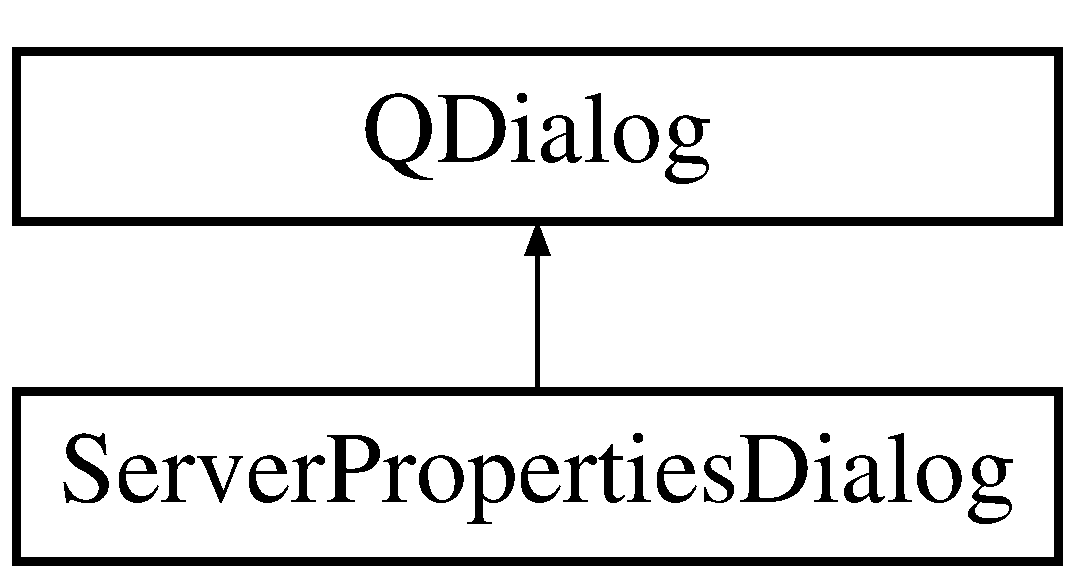
\includegraphics[height=2.000000cm]{classServerPropertiesDialog}
\end{center}
\end{figure}
\subsection*{Public Member Functions}
\begin{DoxyCompactItemize}
\item 
\hyperlink{classServerPropertiesDialog_aedeacbc38d85372d3fc543ca4537ed72}{Server\-Properties\-Dialog} (Q\-Widget $\ast$parent=0)
\item 
\hyperlink{classServerPropertiesDialog_abbf1b205ce936945c54ef51bf638ff07}{$\sim$\-Server\-Properties\-Dialog} ()
\item 
Q\-String \hyperlink{classServerPropertiesDialog_ae2fe6ffc4e0c04a9043a14a96f6aa5e9}{get\-Host\-Name} () const 
\item 
int \hyperlink{classServerPropertiesDialog_a00869f1fe5e8418017acfa6f351020d1}{get\-Port} () const 
\end{DoxyCompactItemize}


\subsection{Detailed Description}
Dialog box to set server properties. 

\begin{DoxyRefDesc}{Deprecated}
\item[\hyperlink{deprecated__deprecated000001}{Deprecated}]This widget was used in an old version of the U\-I and is now no longer present. \end{DoxyRefDesc}


\subsection{Constructor \& Destructor Documentation}
\hypertarget{classServerPropertiesDialog_aedeacbc38d85372d3fc543ca4537ed72}{\index{Server\-Properties\-Dialog@{Server\-Properties\-Dialog}!Server\-Properties\-Dialog@{Server\-Properties\-Dialog}}
\index{Server\-Properties\-Dialog@{Server\-Properties\-Dialog}!ServerPropertiesDialog@{Server\-Properties\-Dialog}}
\subsubsection[{Server\-Properties\-Dialog}]{\setlength{\rightskip}{0pt plus 5cm}Server\-Properties\-Dialog\-::\-Server\-Properties\-Dialog (
\begin{DoxyParamCaption}
\item[{Q\-Widget $\ast$}]{parent = {\ttfamily 0}}
\end{DoxyParamCaption}
)\hspace{0.3cm}{\ttfamily [explicit]}}}\label{classServerPropertiesDialog_aedeacbc38d85372d3fc543ca4537ed72}

\begin{DoxyCode}
5                                                               :
6     QDialog(parent),
7     ui(\textcolor{keyword}{new} Ui::ServerPropertiesDialog),
8     m\_file\_util(\textcolor{keyword}{new} \hyperlink{classServerConfigFileUtil}{ServerConfigFileUtil}),
9     m\_file\_name(QString(\textcolor{stringliteral}{"
      /home/dustin/QtWorkspace/misc-applications/VideoStreamController/Config/server\_config.xml"}))
10 \{
11     ui->setupUi(\textcolor{keyword}{this});
12     connect(\textcolor{keyword}{this}, SIGNAL(accepted()), \textcolor{keyword}{this}, SLOT(acceptedClicked()));
13     \textcolor{comment}{//Attempt to load server properties}
14     \textcolor{keywordtype}{bool} loaded = m\_file\_util->\hyperlink{classServerConfigFileUtil_a9b089be8defbadfd37fcdefee8b22ade}{loadDocument}(m\_file\_name.toStdString().c\_str());
15     \textcolor{keywordflow}{if}(loaded)
16     \{
17         \hyperlink{serverconfigfileutil_8h_a90d1af3762c28656b0507bb3a650f96e}{AddressList} servers = m\_file\_util->\hyperlink{classServerConfigFileUtil_a1eaba4990950df8f21ee8ae99b638a9d}{getServerInfo}();
18         \hyperlink{serverconfigfileutil_8h_aa849a66e29fe72431879f7d9d8ccda63}{AddressListIter} first\_node = servers.begin();
19         m\_port = first\_node->getPort();
20         m\_host\_name = QString(first\_node->getAddress().c\_str());
21         ui->leHost->setText(m\_host\_name);
22         ui->lePort->setText(QString::number(m\_port));
23 
24     \}
25 \}
\end{DoxyCode}
\hypertarget{classServerPropertiesDialog_abbf1b205ce936945c54ef51bf638ff07}{\index{Server\-Properties\-Dialog@{Server\-Properties\-Dialog}!$\sim$\-Server\-Properties\-Dialog@{$\sim$\-Server\-Properties\-Dialog}}
\index{$\sim$\-Server\-Properties\-Dialog@{$\sim$\-Server\-Properties\-Dialog}!ServerPropertiesDialog@{Server\-Properties\-Dialog}}
\subsubsection[{$\sim$\-Server\-Properties\-Dialog}]{\setlength{\rightskip}{0pt plus 5cm}Server\-Properties\-Dialog\-::$\sim$\-Server\-Properties\-Dialog (
\begin{DoxyParamCaption}
{}
\end{DoxyParamCaption}
)}}\label{classServerPropertiesDialog_abbf1b205ce936945c54ef51bf638ff07}

\begin{DoxyCode}
28 \{
29     \textcolor{keyword}{delete} ui;
30     \textcolor{keyword}{delete} m\_file\_util;
31 \}
\end{DoxyCode}


\subsection{Member Function Documentation}
\hypertarget{classServerPropertiesDialog_ae2fe6ffc4e0c04a9043a14a96f6aa5e9}{\index{Server\-Properties\-Dialog@{Server\-Properties\-Dialog}!get\-Host\-Name@{get\-Host\-Name}}
\index{get\-Host\-Name@{get\-Host\-Name}!ServerPropertiesDialog@{Server\-Properties\-Dialog}}
\subsubsection[{get\-Host\-Name}]{\setlength{\rightskip}{0pt plus 5cm}Q\-String Server\-Properties\-Dialog\-::get\-Host\-Name (
\begin{DoxyParamCaption}
{}
\end{DoxyParamCaption}
) const}}\label{classServerPropertiesDialog_ae2fe6ffc4e0c04a9043a14a96f6aa5e9}

\begin{DoxyCode}
34 \{
35     \textcolor{keywordflow}{return} m\_host\_name;
36 \}
\end{DoxyCode}
\hypertarget{classServerPropertiesDialog_a00869f1fe5e8418017acfa6f351020d1}{\index{Server\-Properties\-Dialog@{Server\-Properties\-Dialog}!get\-Port@{get\-Port}}
\index{get\-Port@{get\-Port}!ServerPropertiesDialog@{Server\-Properties\-Dialog}}
\subsubsection[{get\-Port}]{\setlength{\rightskip}{0pt plus 5cm}int Server\-Properties\-Dialog\-::get\-Port (
\begin{DoxyParamCaption}
{}
\end{DoxyParamCaption}
) const}}\label{classServerPropertiesDialog_a00869f1fe5e8418017acfa6f351020d1}

\begin{DoxyCode}
38 \{
39     \textcolor{keywordflow}{return} m\_port;
40 \}
\end{DoxyCode}


The documentation for this class was generated from the following files\-:\begin{DoxyCompactItemize}
\item 
U\-I/\hyperlink{serverpropertiesdialog_8h}{serverpropertiesdialog.\-h}\item 
U\-I/\hyperlink{serverpropertiesdialog_8cpp}{serverpropertiesdialog.\-cpp}\end{DoxyCompactItemize}

\hypertarget{classSocket}{\section{Socket Class Reference}
\label{classSocket}\index{Socket@{Socket}}
}


{\ttfamily \#include $<$socket.\-h$>$}

\subsection*{Public Member Functions}
\begin{DoxyCompactItemize}
\item 
\hyperlink{classSocket_a7c3256c4fc6e2c603df73201049fae5a}{Socket} ()
\item 
\hyperlink{classSocket_aeac4eb6379a543d38ed88977d3b6630a}{$\sim$\-Socket} ()
\item 
bool \hyperlink{classSocket_a7d7e4c8274e8028cc56f5778f98936b1}{Open} (unsigned short port)
\item 
void \hyperlink{classSocket_a4c8ced9a8ce58834191b3b4f2033b173}{Close} ()
\item 
bool \hyperlink{classSocket_ac275fce8d3c3b200e92fd96437673d99}{is\-Open} () const 
\item 
bool \hyperlink{classSocket_a58639d5ede0d7f4ddd8b96ac8c6c0b9b}{Send} (const \hyperlink{classAddress}{Address} \&addr, const void $\ast$data, int size)
\item 
bool \hyperlink{classSocket_a24d0d17efdaab291e81d5d89b463a585}{Receive} (\hyperlink{classAddress}{Address} \&addr, void $\ast$data, int size)
\end{DoxyCompactItemize}


\subsection{Constructor \& Destructor Documentation}
\hypertarget{classSocket_a7c3256c4fc6e2c603df73201049fae5a}{\index{Socket@{Socket}!Socket@{Socket}}
\index{Socket@{Socket}!Socket@{Socket}}
\subsubsection[{Socket}]{\setlength{\rightskip}{0pt plus 5cm}Socket\-::\-Socket (
\begin{DoxyParamCaption}
{}
\end{DoxyParamCaption}
)}}\label{classSocket_a7c3256c4fc6e2c603df73201049fae5a}

\begin{DoxyCode}
16                :
17     m\_isOpen(\textcolor{keyword}{false})
18 \{
19 \}
\end{DoxyCode}
\hypertarget{classSocket_aeac4eb6379a543d38ed88977d3b6630a}{\index{Socket@{Socket}!$\sim$\-Socket@{$\sim$\-Socket}}
\index{$\sim$\-Socket@{$\sim$\-Socket}!Socket@{Socket}}
\subsubsection[{$\sim$\-Socket}]{\setlength{\rightskip}{0pt plus 5cm}Socket\-::$\sim$\-Socket (
\begin{DoxyParamCaption}
{}
\end{DoxyParamCaption}
)}}\label{classSocket_aeac4eb6379a543d38ed88977d3b6630a}

\begin{DoxyCode}
21 \{
22     this->\hyperlink{classSocket_a4c8ced9a8ce58834191b3b4f2033b173}{Close}();
23     \hyperlink{Log_8h_a7cec51f4ce4b22e8c0f256485d57fca7}{INFO}() << \textcolor{stringliteral}{"Destroyed the socket object."};
24 \}
\end{DoxyCode}


\subsection{Member Function Documentation}
\hypertarget{classSocket_a4c8ced9a8ce58834191b3b4f2033b173}{\index{Socket@{Socket}!Close@{Close}}
\index{Close@{Close}!Socket@{Socket}}
\subsubsection[{Close}]{\setlength{\rightskip}{0pt plus 5cm}void Socket\-::\-Close (
\begin{DoxyParamCaption}
{}
\end{DoxyParamCaption}
)}}\label{classSocket_a4c8ced9a8ce58834191b3b4f2033b173}

\begin{DoxyCode}
80 \{
81 \textcolor{preprocessor}{#if defined(Q\_OS\_WIN32)}
82 \textcolor{preprocessor}{}    closesocket(this->m\_handle);
83     WSACleanup();
84 \textcolor{preprocessor}{#elif defined(Q\_OS\_LINUX)}
85 \textcolor{preprocessor}{}    close(this->m\_handle);
86 \textcolor{preprocessor}{#endif}
87 \textcolor{preprocessor}{}
88     \hyperlink{Log_8h_a7cec51f4ce4b22e8c0f256485d57fca7}{INFO}() << \textcolor{stringliteral}{"Closed socket: "} << this->m\_handle;
89     this->m\_isOpen = \textcolor{keyword}{false};
90 \}
\end{DoxyCode}
\hypertarget{classSocket_ac275fce8d3c3b200e92fd96437673d99}{\index{Socket@{Socket}!is\-Open@{is\-Open}}
\index{is\-Open@{is\-Open}!Socket@{Socket}}
\subsubsection[{is\-Open}]{\setlength{\rightskip}{0pt plus 5cm}bool Socket\-::is\-Open (
\begin{DoxyParamCaption}
{}
\end{DoxyParamCaption}
) const}}\label{classSocket_ac275fce8d3c3b200e92fd96437673d99}

\begin{DoxyCode}
94 \{
95     \textcolor{keywordflow}{return} this->m\_isOpen;
96 \}
\end{DoxyCode}
\hypertarget{classSocket_a7d7e4c8274e8028cc56f5778f98936b1}{\index{Socket@{Socket}!Open@{Open}}
\index{Open@{Open}!Socket@{Socket}}
\subsubsection[{Open}]{\setlength{\rightskip}{0pt plus 5cm}bool Socket\-::\-Open (
\begin{DoxyParamCaption}
\item[{unsigned short}]{port}
\end{DoxyParamCaption}
)}}\label{classSocket_a7d7e4c8274e8028cc56f5778f98936b1}

\begin{DoxyCode}
26 \{
27     errno = 0;
28     \textcolor{comment}{//Setting up the windows socket layer}
29 \textcolor{preprocessor}{#ifdef Q\_OS\_WIN32}
30 \textcolor{preprocessor}{}    WSADATA WsaData;
31     \textcolor{keywordflow}{if}(!(WSAStartup(MAKEWORD(2,2), &WsaData) == NO\_ERROR))
32     \{
33         \hyperlink{Log_8h_a1a242c34c5066fb0c62d909f22d3716d}{L\_ERROR}() << \textcolor{stringliteral}{"Unable to initialize windows socket layer..."} << strerror(errno);
34     \}
35 \textcolor{preprocessor}{#endif}
36 \textcolor{preprocessor}{}
37     \textcolor{comment}{//Open a socket}
38     this->m\_handle = socket(AF\_INET, SOCK\_DGRAM, IPPROTO\_UDP);
39     \textcolor{keywordflow}{if}(m\_handle < 0)
40     \{
41         this->m\_isOpen = \textcolor{keyword}{false};
42         \hyperlink{Log_8h_a1a242c34c5066fb0c62d909f22d3716d}{L\_ERROR}() << \textcolor{stringliteral}{"Could not get handle on socket: "} << strerror(errno);
43         \textcolor{keywordflow}{return} \textcolor{keyword}{false};
44     \}
45 
46     \textcolor{comment}{//Bind to a socket on the host}
47     sockaddr\_in address;
48     address.sin\_family = AF\_INET;
49     address.sin\_addr.s\_addr = INADDR\_ANY;
50     address.sin\_port = htons(port);
51 
52     \textcolor{keywordflow}{if}(bind(m\_handle, (\textcolor{keyword}{const} sockaddr *)&address, \textcolor{keyword}{sizeof}(sockaddr\_in)) < 0)
53     \{
54         this->m\_isOpen = \textcolor{keyword}{false};
55         \hyperlink{Log_8h_a1a242c34c5066fb0c62d909f22d3716d}{L\_ERROR}() << \textcolor{stringliteral}{"Could not bind to socket: "} << strerror(errno);
56         \textcolor{keywordflow}{return} \textcolor{keyword}{false};
57     \}
58 
59     \textcolor{comment}{//Set socket non-blocking}
60 \textcolor{preprocessor}{#if defined(Q\_OS\_LINUX)}
61 \textcolor{preprocessor}{}    \textcolor{keywordtype}{int} nonblocking = 1;
62     \textcolor{keywordflow}{if}(fcntl(m\_handle, F\_SETFL, O\_NONBLOCK, nonblocking) == -1)
63     \{
64         this->m\_isOpen = \textcolor{keyword}{false};
65         \hyperlink{Log_8h_a1a242c34c5066fb0c62d909f22d3716d}{L\_ERROR}() << \textcolor{stringliteral}{"Could not set socket non-blocking: "} << strerror(errno);
66         \textcolor{keywordflow}{return} \textcolor{keyword}{false};
67     \}
68 \textcolor{preprocessor}{#elif defined(Q\_OS\_WIN32)}
69 \textcolor{preprocessor}{}    DWORD nonblocking = 1;
70     \textcolor{keywordflow}{if}((ioctlsocket(m\_handle, FIONBIO, &nonblocking) != 0))
71     \{
72         \hyperlink{Log_8h_a1a242c34c5066fb0c62d909f22d3716d}{L\_ERROR}() << \textcolor{stringliteral}{"Could not set non-blocking "} << strerror(errno);
73     \}
74 \textcolor{preprocessor}{#endif}
75 \textcolor{preprocessor}{}    \textcolor{keywordflow}{return} \textcolor{keyword}{true};
76 \}
\end{DoxyCode}
\hypertarget{classSocket_a24d0d17efdaab291e81d5d89b463a585}{\index{Socket@{Socket}!Receive@{Receive}}
\index{Receive@{Receive}!Socket@{Socket}}
\subsubsection[{Receive}]{\setlength{\rightskip}{0pt plus 5cm}bool Socket\-::\-Receive (
\begin{DoxyParamCaption}
\item[{{\bf Address} \&}]{addr, }
\item[{void $\ast$}]{data, }
\item[{int}]{size}
\end{DoxyParamCaption}
)}}\label{classSocket_a24d0d17efdaab291e81d5d89b463a585}

\begin{DoxyCode}
128 \{
129 \textcolor{preprocessor}{#ifdef Q\_OS\_WIN32}
130 \textcolor{preprocessor}{}    \textcolor{keyword}{typedef} \textcolor{keywordtype}{int} socklen\_t;
131 \textcolor{preprocessor}{#endif}
132 \textcolor{preprocessor}{}    sockaddr\_in from;
133     socklen\_t fromLength = \textcolor{keyword}{sizeof}(from);
134 
135     \textcolor{keywordtype}{int} received\_bytes = recvfrom(this->m\_handle, (\textcolor{keywordtype}{char} *) data, size, 0, (sockaddr *)&from, &fromLength);
136 
137     \textcolor{keywordflow}{if}(received\_bytes <= 0)
138         \textcolor{keywordflow}{return} \textcolor{keyword}{false};
139 
140     \textcolor{keywordtype}{string} address(inet\_ntoa(from.sin\_addr));
141     \textcolor{keywordtype}{unsigned} \textcolor{keywordtype}{int} port = ntohs(from.sin\_port);
142     addr.\hyperlink{classAddress_a43ba5f8001b7e729b83b1b9299294495}{setAddress}(address);
143     addr.\hyperlink{classAddress_ad73c29200f7d63641e48ebfc16efaf75}{setPort}(port);
144 
145     \textcolor{keywordflow}{return} \textcolor{keyword}{true};
146 \}
\end{DoxyCode}
\hypertarget{classSocket_a58639d5ede0d7f4ddd8b96ac8c6c0b9b}{\index{Socket@{Socket}!Send@{Send}}
\index{Send@{Send}!Socket@{Socket}}
\subsubsection[{Send}]{\setlength{\rightskip}{0pt plus 5cm}bool Socket\-::\-Send (
\begin{DoxyParamCaption}
\item[{const {\bf Address} \&}]{addr, }
\item[{const void $\ast$}]{data, }
\item[{int}]{size}
\end{DoxyParamCaption}
)}}\label{classSocket_a58639d5ede0d7f4ddd8b96ac8c6c0b9b}

\begin{DoxyCode}
99 \{
100     \hyperlink{Log_8h_a7cec51f4ce4b22e8c0f256485d57fca7}{INFO}() << \textcolor{stringliteral}{"Sending packet with size: "} << size;
101     \textcolor{comment}{//Set up the destination address}
102     sockaddr\_in dest;
103     dest.sin\_family = AF\_INET;
104     dest.sin\_addr.s\_addr = inet\_addr(addr.\hyperlink{classAddress_aa84d076d4adf5cac8381146fcf261af7}{getAddress}().c\_str());
105     dest.sin\_port = htons((\textcolor{keywordtype}{unsigned} \textcolor{keywordtype}{short})addr.\hyperlink{classAddress_aa7d7e4b33ab75aa3ca146341a5e74472}{getPort}());
106 
107     \textcolor{keywordtype}{int} sent\_bytes = sendto(this->m\_handle, (\textcolor{keyword}{const} \textcolor{keywordtype}{char} *)data, size, 0, (sockaddr *)&dest, \textcolor{keyword}{sizeof}(
      sockaddr\_in));
108 
109     \textcolor{keywordflow}{if}(sent\_bytes != size)
110     \{
111         \hyperlink{Log_8h_a1a242c34c5066fb0c62d909f22d3716d}{L\_ERROR}() << \textcolor{stringliteral}{"RETURNED SIZE DOES NOT MATCH SIZE OF PACKET!"};
112         \textcolor{keywordflow}{return} \textcolor{keyword}{false};
113     \}
114     \textcolor{keywordflow}{else}
115     \{
116         \hyperlink{Log_8h_a7cec51f4ce4b22e8c0f256485d57fca7}{INFO}() << \textcolor{stringliteral}{"Packet sent sucessfully."};
117         \textcolor{keywordflow}{if}(size < 50)
118         \{
119             \hyperlink{Log_8h_a7cec51f4ce4b22e8c0f256485d57fca7}{INFO}() << \textcolor{stringliteral}{"Payload: "} << (\textcolor{keyword}{const} \textcolor{keywordtype}{char} *)data;
120         \}
121         \textcolor{keywordflow}{return} \textcolor{keyword}{true};
122     \}
123 
124 \}
\end{DoxyCode}


The documentation for this class was generated from the following files\-:\begin{DoxyCompactItemize}
\item 
Network/\hyperlink{socket_8h}{socket.\-h}\item 
Network/\hyperlink{socket_8cpp}{socket.\-cpp}\end{DoxyCompactItemize}

\hypertarget{structstrconv__attribute__impl}{\section{strconv\-\_\-attribute\-\_\-impl$<$ opt\-\_\-escape $>$ Struct Template Reference}
\label{structstrconv__attribute__impl}\index{strconv\-\_\-attribute\-\_\-impl$<$ opt\-\_\-escape $>$@{strconv\-\_\-attribute\-\_\-impl$<$ opt\-\_\-escape $>$}}
}
\subsection*{Static Public Member Functions}
\begin{DoxyCompactItemize}
\item 
static char\-\_\-t $\ast$ \hyperlink{structstrconv__attribute__impl_a9b7f8b1e860c5d022dbd29f9a89e9e27}{parse\-\_\-wnorm} (char\-\_\-t $\ast$s, char\-\_\-t end\-\_\-quote)
\item 
static char\-\_\-t $\ast$ \hyperlink{structstrconv__attribute__impl_a2d39998b79896af7c53c5f3dc22a526b}{parse\-\_\-wconv} (char\-\_\-t $\ast$s, char\-\_\-t end\-\_\-quote)
\item 
static char\-\_\-t $\ast$ \hyperlink{structstrconv__attribute__impl_a0f57ee9d69b9d626765f4a9c8af6df2e}{parse\-\_\-eol} (char\-\_\-t $\ast$s, char\-\_\-t end\-\_\-quote)
\item 
static char\-\_\-t $\ast$ \hyperlink{structstrconv__attribute__impl_a8358dc980178e55c8669b9dcd04872d7}{parse\-\_\-simple} (char\-\_\-t $\ast$s, char\-\_\-t end\-\_\-quote)
\end{DoxyCompactItemize}


\subsection{Member Function Documentation}
\hypertarget{structstrconv__attribute__impl_a0f57ee9d69b9d626765f4a9c8af6df2e}{\index{strconv\-\_\-attribute\-\_\-impl@{strconv\-\_\-attribute\-\_\-impl}!parse\-\_\-eol@{parse\-\_\-eol}}
\index{parse\-\_\-eol@{parse\-\_\-eol}!strconv_attribute_impl@{strconv\-\_\-attribute\-\_\-impl}}
\subsubsection[{parse\-\_\-eol}]{\setlength{\rightskip}{0pt plus 5cm}template$<$typename opt\-\_\-escape $>$ static char\-\_\-t$\ast$ {\bf strconv\-\_\-attribute\-\_\-impl}$<$ opt\-\_\-escape $>$\-::parse\-\_\-eol (
\begin{DoxyParamCaption}
\item[{char\-\_\-t $\ast$}]{s, }
\item[{char\-\_\-t}]{end\-\_\-quote}
\end{DoxyParamCaption}
)\hspace{0.3cm}{\ttfamily [inline]}, {\ttfamily [static]}}}\label{structstrconv__attribute__impl_a0f57ee9d69b9d626765f4a9c8af6df2e}

\begin{DoxyCode}
1957         \{
1958             \hyperlink{structgap}{gap} g;
1959 
1960             \textcolor{keywordflow}{while} (\textcolor{keyword}{true})
1961             \{
1962                 \textcolor{keywordflow}{while} (!\hyperlink{pugixml_8cpp_a2adf5ae9b7505408a18e9f3bb1b3d332}{PUGI\_\_IS\_CHARTYPE}(*s, \hyperlink{pugixml_8cpp_ae83a55e5947d28c62625b690b1484108a884462ea84ab1e7745a2bf69fc2edf75}{ct\_parse\_attr})) ++s;
1963                 
1964                 \textcolor{keywordflow}{if} (*s == end\_quote)
1965                 \{
1966                     *g.\hyperlink{structgap_a176c58ee8d57c41b91ae9f00d5e8cab5}{flush}(s) = 0;
1967                 
1968                     \textcolor{keywordflow}{return} s + 1;
1969                 \}
1970                 \textcolor{keywordflow}{else} \textcolor{keywordflow}{if} (*s == \textcolor{charliteral}{'\(\backslash\)r'})
1971                 \{
1972                     *s++ = \textcolor{charliteral}{'\(\backslash\)n'};
1973                     
1974                     \textcolor{keywordflow}{if} (*s == \textcolor{charliteral}{'\(\backslash\)n'}) g.\hyperlink{structgap_a9c0d0b12bc778c8439c8aec7747ab2b0}{push}(s, 1);
1975                 \}
1976                 \textcolor{keywordflow}{else} \textcolor{keywordflow}{if} (opt\_escape::value && *s == \textcolor{charliteral}{'&'})
1977                 \{
1978                     s = \hyperlink{pugixml_8cpp_a7cf2b6da7b109a11f8cb1c7e1a09bf7e}{strconv\_escape}(s, g);
1979                 \}
1980                 \textcolor{keywordflow}{else} \textcolor{keywordflow}{if} (!*s)
1981                 \{
1982                     \textcolor{keywordflow}{return} 0;
1983                 \}
1984                 \textcolor{keywordflow}{else} ++s;
1985             \}
1986         \}
\end{DoxyCode}
\hypertarget{structstrconv__attribute__impl_a8358dc980178e55c8669b9dcd04872d7}{\index{strconv\-\_\-attribute\-\_\-impl@{strconv\-\_\-attribute\-\_\-impl}!parse\-\_\-simple@{parse\-\_\-simple}}
\index{parse\-\_\-simple@{parse\-\_\-simple}!strconv_attribute_impl@{strconv\-\_\-attribute\-\_\-impl}}
\subsubsection[{parse\-\_\-simple}]{\setlength{\rightskip}{0pt plus 5cm}template$<$typename opt\-\_\-escape $>$ static char\-\_\-t$\ast$ {\bf strconv\-\_\-attribute\-\_\-impl}$<$ opt\-\_\-escape $>$\-::parse\-\_\-simple (
\begin{DoxyParamCaption}
\item[{char\-\_\-t $\ast$}]{s, }
\item[{char\-\_\-t}]{end\-\_\-quote}
\end{DoxyParamCaption}
)\hspace{0.3cm}{\ttfamily [inline]}, {\ttfamily [static]}}}\label{structstrconv__attribute__impl_a8358dc980178e55c8669b9dcd04872d7}

\begin{DoxyCode}
1989         \{
1990             \hyperlink{structgap}{gap} g;
1991 
1992             \textcolor{keywordflow}{while} (\textcolor{keyword}{true})
1993             \{
1994                 \textcolor{keywordflow}{while} (!\hyperlink{pugixml_8cpp_a2adf5ae9b7505408a18e9f3bb1b3d332}{PUGI\_\_IS\_CHARTYPE}(*s, \hyperlink{pugixml_8cpp_ae83a55e5947d28c62625b690b1484108a884462ea84ab1e7745a2bf69fc2edf75}{ct\_parse\_attr})) ++s;
1995                 
1996                 \textcolor{keywordflow}{if} (*s == end\_quote)
1997                 \{
1998                     *g.\hyperlink{structgap_a176c58ee8d57c41b91ae9f00d5e8cab5}{flush}(s) = 0;
1999                 
2000                     \textcolor{keywordflow}{return} s + 1;
2001                 \}
2002                 \textcolor{keywordflow}{else} \textcolor{keywordflow}{if} (opt\_escape::value && *s == \textcolor{charliteral}{'&'})
2003                 \{
2004                     s = \hyperlink{pugixml_8cpp_a7cf2b6da7b109a11f8cb1c7e1a09bf7e}{strconv\_escape}(s, g);
2005                 \}
2006                 \textcolor{keywordflow}{else} \textcolor{keywordflow}{if} (!*s)
2007                 \{
2008                     \textcolor{keywordflow}{return} 0;
2009                 \}
2010                 \textcolor{keywordflow}{else} ++s;
2011             \}
2012         \}
\end{DoxyCode}
\hypertarget{structstrconv__attribute__impl_a2d39998b79896af7c53c5f3dc22a526b}{\index{strconv\-\_\-attribute\-\_\-impl@{strconv\-\_\-attribute\-\_\-impl}!parse\-\_\-wconv@{parse\-\_\-wconv}}
\index{parse\-\_\-wconv@{parse\-\_\-wconv}!strconv_attribute_impl@{strconv\-\_\-attribute\-\_\-impl}}
\subsubsection[{parse\-\_\-wconv}]{\setlength{\rightskip}{0pt plus 5cm}template$<$typename opt\-\_\-escape $>$ static char\-\_\-t$\ast$ {\bf strconv\-\_\-attribute\-\_\-impl}$<$ opt\-\_\-escape $>$\-::parse\-\_\-wconv (
\begin{DoxyParamCaption}
\item[{char\-\_\-t $\ast$}]{s, }
\item[{char\-\_\-t}]{end\-\_\-quote}
\end{DoxyParamCaption}
)\hspace{0.3cm}{\ttfamily [inline]}, {\ttfamily [static]}}}\label{structstrconv__attribute__impl_a2d39998b79896af7c53c5f3dc22a526b}

\begin{DoxyCode}
1921         \{
1922             \hyperlink{structgap}{gap} g;
1923 
1924             \textcolor{keywordflow}{while} (\textcolor{keyword}{true})
1925             \{
1926                 \textcolor{keywordflow}{while} (!\hyperlink{pugixml_8cpp_a2adf5ae9b7505408a18e9f3bb1b3d332}{PUGI\_\_IS\_CHARTYPE}(*s, \hyperlink{pugixml_8cpp_ae83a55e5947d28c62625b690b1484108a8ac9b7ded4827803524b87f772f17c51}{ct\_parse\_attr\_ws})) ++s;
1927                 
1928                 \textcolor{keywordflow}{if} (*s == end\_quote)
1929                 \{
1930                     *g.\hyperlink{structgap_a176c58ee8d57c41b91ae9f00d5e8cab5}{flush}(s) = 0;
1931                 
1932                     \textcolor{keywordflow}{return} s + 1;
1933                 \}
1934                 \textcolor{keywordflow}{else} \textcolor{keywordflow}{if} (\hyperlink{pugixml_8cpp_a2adf5ae9b7505408a18e9f3bb1b3d332}{PUGI\_\_IS\_CHARTYPE}(*s, \hyperlink{pugixml_8cpp_ae83a55e5947d28c62625b690b1484108ac957a1774b6a4430e583bcb881909372}{ct\_space}))
1935                 \{
1936                     \textcolor{keywordflow}{if} (*s == \textcolor{charliteral}{'\(\backslash\)r'})
1937                     \{
1938                         *s++ = \textcolor{charliteral}{' '};
1939                 
1940                         \textcolor{keywordflow}{if} (*s == \textcolor{charliteral}{'\(\backslash\)n'}) g.\hyperlink{structgap_a9c0d0b12bc778c8439c8aec7747ab2b0}{push}(s, 1);
1941                     \}
1942                     \textcolor{keywordflow}{else} *s++ = \textcolor{charliteral}{' '};
1943                 \}
1944                 \textcolor{keywordflow}{else} \textcolor{keywordflow}{if} (opt\_escape::value && *s == \textcolor{charliteral}{'&'})
1945                 \{
1946                     s = \hyperlink{pugixml_8cpp_a7cf2b6da7b109a11f8cb1c7e1a09bf7e}{strconv\_escape}(s, g);
1947                 \}
1948                 \textcolor{keywordflow}{else} \textcolor{keywordflow}{if} (!*s)
1949                 \{
1950                     \textcolor{keywordflow}{return} 0;
1951                 \}
1952                 \textcolor{keywordflow}{else} ++s;
1953             \}
1954         \}
\end{DoxyCode}
\hypertarget{structstrconv__attribute__impl_a9b7f8b1e860c5d022dbd29f9a89e9e27}{\index{strconv\-\_\-attribute\-\_\-impl@{strconv\-\_\-attribute\-\_\-impl}!parse\-\_\-wnorm@{parse\-\_\-wnorm}}
\index{parse\-\_\-wnorm@{parse\-\_\-wnorm}!strconv_attribute_impl@{strconv\-\_\-attribute\-\_\-impl}}
\subsubsection[{parse\-\_\-wnorm}]{\setlength{\rightskip}{0pt plus 5cm}template$<$typename opt\-\_\-escape $>$ static char\-\_\-t$\ast$ {\bf strconv\-\_\-attribute\-\_\-impl}$<$ opt\-\_\-escape $>$\-::parse\-\_\-wnorm (
\begin{DoxyParamCaption}
\item[{char\-\_\-t $\ast$}]{s, }
\item[{char\-\_\-t}]{end\-\_\-quote}
\end{DoxyParamCaption}
)\hspace{0.3cm}{\ttfamily [inline]}, {\ttfamily [static]}}}\label{structstrconv__attribute__impl_a9b7f8b1e860c5d022dbd29f9a89e9e27}

\begin{DoxyCode}
1869         \{
1870             \hyperlink{structgap}{gap} g;
1871 
1872             \textcolor{comment}{// trim leading whitespaces}
1873             \textcolor{keywordflow}{if} (\hyperlink{pugixml_8cpp_a2adf5ae9b7505408a18e9f3bb1b3d332}{PUGI\_\_IS\_CHARTYPE}(*s, \hyperlink{pugixml_8cpp_ae83a55e5947d28c62625b690b1484108ac957a1774b6a4430e583bcb881909372}{ct\_space}))
1874             \{
1875                 \hyperlink{namespacepugi_aef5a7a62cba0507542220ea15afe39df}{char\_t}* str = s;
1876                 
1877                 \textcolor{keywordflow}{do} ++str;
1878                 \textcolor{keywordflow}{while} (\hyperlink{pugixml_8cpp_a2adf5ae9b7505408a18e9f3bb1b3d332}{PUGI\_\_IS\_CHARTYPE}(*str, \hyperlink{pugixml_8cpp_ae83a55e5947d28c62625b690b1484108ac957a1774b6a4430e583bcb881909372}{ct\_space}));
1879                 
1880                 g.\hyperlink{structgap_a9c0d0b12bc778c8439c8aec7747ab2b0}{push}(s, str - s);
1881             \}
1882 
1883             \textcolor{keywordflow}{while} (\textcolor{keyword}{true})
1884             \{
1885                 \textcolor{keywordflow}{while} (!\hyperlink{pugixml_8cpp_a2adf5ae9b7505408a18e9f3bb1b3d332}{PUGI\_\_IS\_CHARTYPE}(*s, \hyperlink{pugixml_8cpp_ae83a55e5947d28c62625b690b1484108a8ac9b7ded4827803524b87f772f17c51}{ct\_parse\_attr\_ws} | 
      \hyperlink{pugixml_8cpp_ae83a55e5947d28c62625b690b1484108ac957a1774b6a4430e583bcb881909372}{ct\_space})) ++s;
1886                 
1887                 \textcolor{keywordflow}{if} (*s == end\_quote)
1888                 \{
1889                     \hyperlink{namespacepugi_aef5a7a62cba0507542220ea15afe39df}{char\_t}* str = g.\hyperlink{structgap_a176c58ee8d57c41b91ae9f00d5e8cab5}{flush}(s);
1890                     
1891                     \textcolor{keywordflow}{do} *str-- = 0;
1892                     \textcolor{keywordflow}{while} (\hyperlink{pugixml_8cpp_a2adf5ae9b7505408a18e9f3bb1b3d332}{PUGI\_\_IS\_CHARTYPE}(*str, \hyperlink{pugixml_8cpp_ae83a55e5947d28c62625b690b1484108ac957a1774b6a4430e583bcb881909372}{ct\_space}));
1893                 
1894                     \textcolor{keywordflow}{return} s + 1;
1895                 \}
1896                 \textcolor{keywordflow}{else} \textcolor{keywordflow}{if} (\hyperlink{pugixml_8cpp_a2adf5ae9b7505408a18e9f3bb1b3d332}{PUGI\_\_IS\_CHARTYPE}(*s, \hyperlink{pugixml_8cpp_ae83a55e5947d28c62625b690b1484108ac957a1774b6a4430e583bcb881909372}{ct\_space}))
1897                 \{
1898                     *s++ = \textcolor{charliteral}{' '};
1899         
1900                     \textcolor{keywordflow}{if} (\hyperlink{pugixml_8cpp_a2adf5ae9b7505408a18e9f3bb1b3d332}{PUGI\_\_IS\_CHARTYPE}(*s, \hyperlink{pugixml_8cpp_ae83a55e5947d28c62625b690b1484108ac957a1774b6a4430e583bcb881909372}{ct\_space}))
1901                     \{
1902                         \hyperlink{namespacepugi_aef5a7a62cba0507542220ea15afe39df}{char\_t}* str = s + 1;
1903                         \textcolor{keywordflow}{while} (\hyperlink{pugixml_8cpp_a2adf5ae9b7505408a18e9f3bb1b3d332}{PUGI\_\_IS\_CHARTYPE}(*str, \hyperlink{pugixml_8cpp_ae83a55e5947d28c62625b690b1484108ac957a1774b6a4430e583bcb881909372}{ct\_space})) ++str;
1904                         
1905                         g.\hyperlink{structgap_a9c0d0b12bc778c8439c8aec7747ab2b0}{push}(s, str - s);
1906                     \}
1907                 \}
1908                 \textcolor{keywordflow}{else} \textcolor{keywordflow}{if} (opt\_escape::value && *s == \textcolor{charliteral}{'&'})
1909                 \{
1910                     s = \hyperlink{pugixml_8cpp_a7cf2b6da7b109a11f8cb1c7e1a09bf7e}{strconv\_escape}(s, g);
1911                 \}
1912                 \textcolor{keywordflow}{else} \textcolor{keywordflow}{if} (!*s)
1913                 \{
1914                     \textcolor{keywordflow}{return} 0;
1915                 \}
1916                 \textcolor{keywordflow}{else} ++s;
1917             \}
1918         \}
\end{DoxyCode}


The documentation for this struct was generated from the following file\-:\begin{DoxyCompactItemize}
\item 
Third\-Party/pugixml/\hyperlink{pugixml_8cpp}{pugixml.\-cpp}\end{DoxyCompactItemize}

\hypertarget{structstrconv__pcdata__impl}{\section{strconv\-\_\-pcdata\-\_\-impl$<$ opt\-\_\-eol, opt\-\_\-escape $>$ Struct Template Reference}
\label{structstrconv__pcdata__impl}\index{strconv\-\_\-pcdata\-\_\-impl$<$ opt\-\_\-eol, opt\-\_\-escape $>$@{strconv\-\_\-pcdata\-\_\-impl$<$ opt\-\_\-eol, opt\-\_\-escape $>$}}
}
\subsection*{Static Public Member Functions}
\begin{DoxyCompactItemize}
\item 
static char\-\_\-t $\ast$ \hyperlink{structstrconv__pcdata__impl_a0aa794c648c72338d92b86c95c681b32}{parse} (char\-\_\-t $\ast$s)
\end{DoxyCompactItemize}


\subsection{Member Function Documentation}
\hypertarget{structstrconv__pcdata__impl_a0aa794c648c72338d92b86c95c681b32}{\index{strconv\-\_\-pcdata\-\_\-impl@{strconv\-\_\-pcdata\-\_\-impl}!parse@{parse}}
\index{parse@{parse}!strconv_pcdata_impl@{strconv\-\_\-pcdata\-\_\-impl}}
\subsubsection[{parse}]{\setlength{\rightskip}{0pt plus 5cm}template$<$typename opt\-\_\-eol , typename opt\-\_\-escape $>$ static char\-\_\-t$\ast$ {\bf strconv\-\_\-pcdata\-\_\-impl}$<$ opt\-\_\-eol, opt\-\_\-escape $>$\-::parse (
\begin{DoxyParamCaption}
\item[{char\-\_\-t $\ast$}]{s}
\end{DoxyParamCaption}
)\hspace{0.3cm}{\ttfamily [inline]}, {\ttfamily [static]}}}\label{structstrconv__pcdata__impl_a0aa794c648c72338d92b86c95c681b32}

\begin{DoxyCode}
1818         \{
1819             \hyperlink{structgap}{gap} g;
1820             
1821             \textcolor{keywordflow}{while} (\textcolor{keyword}{true})
1822             \{
1823                 \textcolor{keywordflow}{while} (!\hyperlink{pugixml_8cpp_a2adf5ae9b7505408a18e9f3bb1b3d332}{PUGI\_\_IS\_CHARTYPE}(*s, \hyperlink{pugixml_8cpp_ae83a55e5947d28c62625b690b1484108aa0f09a99c3d76641d00d0ad11f4f2fa1}{ct\_parse\_pcdata})) ++s;
1824                     
1825                 \textcolor{keywordflow}{if} (*s == \textcolor{charliteral}{'<'}) \textcolor{comment}{// PCDATA ends here}
1826                 \{
1827                     *g.\hyperlink{structgap_a176c58ee8d57c41b91ae9f00d5e8cab5}{flush}(s) = 0;
1828                     
1829                     \textcolor{keywordflow}{return} s + 1;
1830                 \}
1831                 \textcolor{keywordflow}{else} \textcolor{keywordflow}{if} (opt\_eol::value && *s == \textcolor{charliteral}{'\(\backslash\)r'}) \textcolor{comment}{// Either a single 0x0d or 0x0d 0x0a pair}
1832                 \{
1833                     *s++ = \textcolor{charliteral}{'\(\backslash\)n'}; \textcolor{comment}{// replace first one with 0x0a}
1834                     
1835                     \textcolor{keywordflow}{if} (*s == \textcolor{charliteral}{'\(\backslash\)n'}) g.\hyperlink{structgap_a9c0d0b12bc778c8439c8aec7747ab2b0}{push}(s, 1);
1836                 \}
1837                 \textcolor{keywordflow}{else} \textcolor{keywordflow}{if} (opt\_escape::value && *s == \textcolor{charliteral}{'&'})
1838                 \{
1839                     s = \hyperlink{pugixml_8cpp_a7cf2b6da7b109a11f8cb1c7e1a09bf7e}{strconv\_escape}(s, g);
1840                 \}
1841                 \textcolor{keywordflow}{else} \textcolor{keywordflow}{if} (*s == 0)
1842                 \{
1843                     \textcolor{keywordflow}{return} s;
1844                 \}
1845                 \textcolor{keywordflow}{else} ++s;
1846             \}
1847         \}
\end{DoxyCode}


The documentation for this struct was generated from the following file\-:\begin{DoxyCompactItemize}
\item 
Third\-Party/pugixml/\hyperlink{pugixml_8cpp}{pugixml.\-cpp}\end{DoxyCompactItemize}

\hypertarget{classStreamerTextEdit}{\section{Streamer\-Text\-Edit Class Reference}
\label{classStreamerTextEdit}\index{Streamer\-Text\-Edit@{Streamer\-Text\-Edit}}
}


A text edit widget that will keep track of command history.  




{\ttfamily \#include $<$streamertextedit.\-h$>$}

Inheritance diagram for Streamer\-Text\-Edit\-:\begin{figure}[H]
\begin{center}
\leavevmode
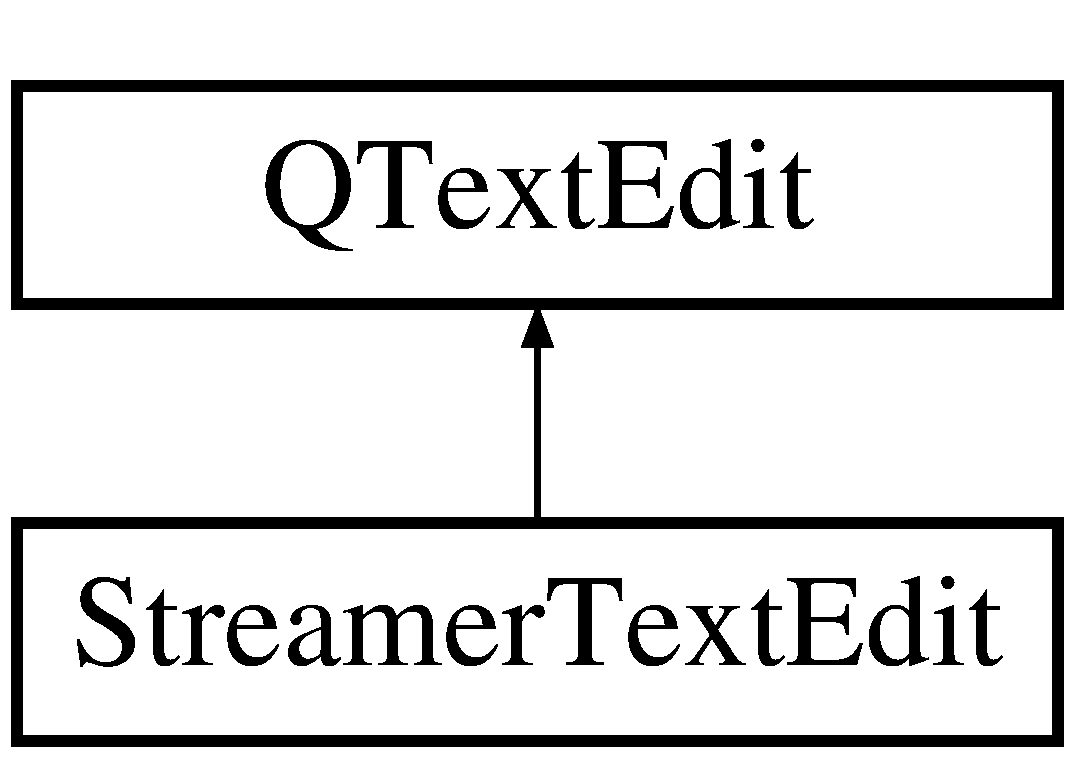
\includegraphics[height=2.000000cm]{classStreamerTextEdit}
\end{center}
\end{figure}
\subsection*{Signals}
\begin{DoxyCompactItemize}
\item 
void \hyperlink{classStreamerTextEdit_aef9c5b51fb00edb2f984128e612629be}{enter\-Pressed} ()
\end{DoxyCompactItemize}
\subsection*{Public Member Functions}
\begin{DoxyCompactItemize}
\item 
\hyperlink{classStreamerTextEdit_a92180ec1922ebb95e6eee9f6463a4190}{Streamer\-Text\-Edit} (Q\-Widget $\ast$parent=0)
\item 
void \hyperlink{classStreamerTextEdit_ac89b399e38a953a0a1835259e91881df}{add\-Command\-To\-List} (\hyperlink{namespaceMainWindowUI_ab4a56a6d14c3fc1c53d1f1373a9033d3}{Main\-Window\-U\-I\-::\-Command\-List\-Item} cmd)
\end{DoxyCompactItemize}
\subsection*{Protected Member Functions}
\begin{DoxyCompactItemize}
\item 
void \hyperlink{classStreamerTextEdit_ad30da0518b808ace5b97f0a160a2f89c}{key\-Press\-Event} (Q\-Key\-Event $\ast$e)
\end{DoxyCompactItemize}


\subsection{Detailed Description}
A text edit widget that will keep track of command history. 

\begin{DoxyRefDesc}{Deprecated}
\item[\hyperlink{deprecated__deprecated000002}{Deprecated}]This widget is no longer used and is part of an older version of the U\-I. \end{DoxyRefDesc}


\subsection{Constructor \& Destructor Documentation}
\hypertarget{classStreamerTextEdit_a92180ec1922ebb95e6eee9f6463a4190}{\index{Streamer\-Text\-Edit@{Streamer\-Text\-Edit}!Streamer\-Text\-Edit@{Streamer\-Text\-Edit}}
\index{Streamer\-Text\-Edit@{Streamer\-Text\-Edit}!StreamerTextEdit@{Streamer\-Text\-Edit}}
\subsubsection[{Streamer\-Text\-Edit}]{\setlength{\rightskip}{0pt plus 5cm}Streamer\-Text\-Edit\-::\-Streamer\-Text\-Edit (
\begin{DoxyParamCaption}
\item[{Q\-Widget $\ast$}]{parent = {\ttfamily 0}}
\end{DoxyParamCaption}
)\hspace{0.3cm}{\ttfamily [explicit]}}}\label{classStreamerTextEdit_a92180ec1922ebb95e6eee9f6463a4190}

\begin{DoxyCode}
5                                                   :
6     QTextEdit(parent),
7     m\_commands()
8 \{   
9     \textcolor{comment}{//Initialize list of commands}
10     m\_commands.clear();
11     m\_commands.push\_front(\textcolor{stringliteral}{"<Enter command>"});
12     this->m\_last\_command = this->m\_commands.begin();
13 
14     \hyperlink{namespaceMainWindowUI_ab4a56a6d14c3fc1c53d1f1373a9033d3}{MainWindowUI::CommandListItem} selected = *(m\_last\_command);
15     this->setText(selected.c\_str());
16 
17 
18 \}
\end{DoxyCode}


\subsection{Member Function Documentation}
\hypertarget{classStreamerTextEdit_ac89b399e38a953a0a1835259e91881df}{\index{Streamer\-Text\-Edit@{Streamer\-Text\-Edit}!add\-Command\-To\-List@{add\-Command\-To\-List}}
\index{add\-Command\-To\-List@{add\-Command\-To\-List}!StreamerTextEdit@{Streamer\-Text\-Edit}}
\subsubsection[{add\-Command\-To\-List}]{\setlength{\rightskip}{0pt plus 5cm}void Streamer\-Text\-Edit\-::add\-Command\-To\-List (
\begin{DoxyParamCaption}
\item[{{\bf Main\-Window\-U\-I\-::\-Command\-List\-Item}}]{cmd}
\end{DoxyParamCaption}
)}}\label{classStreamerTextEdit_ac89b399e38a953a0a1835259e91881df}

\begin{DoxyCode}
21 \{
22     this->m\_commands.push\_front(cmd);
23 \}
\end{DoxyCode}
\hypertarget{classStreamerTextEdit_aef9c5b51fb00edb2f984128e612629be}{\index{Streamer\-Text\-Edit@{Streamer\-Text\-Edit}!enter\-Pressed@{enter\-Pressed}}
\index{enter\-Pressed@{enter\-Pressed}!StreamerTextEdit@{Streamer\-Text\-Edit}}
\subsubsection[{enter\-Pressed}]{\setlength{\rightskip}{0pt plus 5cm}void Streamer\-Text\-Edit\-::enter\-Pressed (
\begin{DoxyParamCaption}
{}
\end{DoxyParamCaption}
)\hspace{0.3cm}{\ttfamily [signal]}}}\label{classStreamerTextEdit_aef9c5b51fb00edb2f984128e612629be}
\hypertarget{classStreamerTextEdit_ad30da0518b808ace5b97f0a160a2f89c}{\index{Streamer\-Text\-Edit@{Streamer\-Text\-Edit}!key\-Press\-Event@{key\-Press\-Event}}
\index{key\-Press\-Event@{key\-Press\-Event}!StreamerTextEdit@{Streamer\-Text\-Edit}}
\subsubsection[{key\-Press\-Event}]{\setlength{\rightskip}{0pt plus 5cm}void Streamer\-Text\-Edit\-::key\-Press\-Event (
\begin{DoxyParamCaption}
\item[{Q\-Key\-Event $\ast$}]{e}
\end{DoxyParamCaption}
)\hspace{0.3cm}{\ttfamily [protected]}}}\label{classStreamerTextEdit_ad30da0518b808ace5b97f0a160a2f89c}

\begin{DoxyCode}
26 \{
27     \textcolor{comment}{//Determine which Key was pressed}
28     \textcolor{keywordflow}{if}(e->key() == Qt::Key\_Up)
29     \{
30         \hyperlink{Log_8h_a7cec51f4ce4b22e8c0f256485d57fca7}{INFO}() << \textcolor{stringliteral}{"Up arrow pressed."};
31         \textcolor{keywordflow}{if}(this->toPlainText().compare(\textcolor{stringliteral}{""}) == 0)
32         \{
33             this->m\_last\_command = this->m\_commands.begin();
34         \}
35         \textcolor{keywordflow}{else}
36         \{
37             this->m\_last\_command++;
38             \textcolor{comment}{//Iterate back to beginning of list}
39             \textcolor{keywordflow}{if}(this->m\_last\_command == m\_commands.end())
40                 m\_last\_command = m\_commands.begin();
41         \}
42         \hyperlink{namespaceMainWindowUI_ab4a56a6d14c3fc1c53d1f1373a9033d3}{MainWindowUI::CommandListItem}& selected = *(m\_last\_command);
43         this->setText(selected.c\_str());
44     \}
45     \textcolor{keywordflow}{else} \textcolor{keywordflow}{if}(e->key() == Qt::Key\_Down)
46     \{
47         \hyperlink{Log_8h_a7cec51f4ce4b22e8c0f256485d57fca7}{INFO}() << \textcolor{stringliteral}{"Down arrow pressed."};
48 
49         \textcolor{comment}{//Iterate back to beginning of list}
50         \textcolor{keywordflow}{if}(this->m\_last\_command == m\_commands.begin())
51         \{
52             this->setText(\textcolor{stringliteral}{""});
53         \}
54         \textcolor{keywordflow}{else}
55         \{
56             this->m\_last\_command--;
57 
58             \hyperlink{namespaceMainWindowUI_ab4a56a6d14c3fc1c53d1f1373a9033d3}{MainWindowUI::CommandListItem}& selected = *(m\_last\_command);
59             this->setText(selected.c\_str());
60         \}
61     \}
62     \textcolor{keywordflow}{else} \textcolor{keywordflow}{if}(e->key() == Qt::Key\_Enter)
63     \{
64         \textcolor{comment}{//Emit the clicked button signal}
65         emit \hyperlink{classStreamerTextEdit_aef9c5b51fb00edb2f984128e612629be}{enterPressed}();
66     \}
67     \textcolor{keywordflow}{else}
68     \{
69         QTextEdit::keyPressEvent(e);
70     \}
71 
72 \}
\end{DoxyCode}


The documentation for this class was generated from the following files\-:\begin{DoxyCompactItemize}
\item 
U\-I/\hyperlink{streamertextedit_8h}{streamertextedit.\-h}\item 
U\-I/\hyperlink{streamertextedit_8cpp}{streamertextedit.\-cpp}\end{DoxyCompactItemize}

\hypertarget{classTCPClient}{\section{T\-C\-P\-Client Class Reference}
\label{classTCPClient}\index{T\-C\-P\-Client@{T\-C\-P\-Client}}
}


This class defines a T\-C\-P client that will send requests to and receive responses from a specified server.  




{\ttfamily \#include $<$tcpclient.\-h$>$}

\subsection*{Public Member Functions}
\begin{DoxyCompactItemize}
\item 
\hyperlink{classTCPClient_ad37bba4f2ebcc899b9871656802dcbe9}{T\-C\-P\-Client} ()
\begin{DoxyCompactList}\small\item\em Default value constructor. \end{DoxyCompactList}\item 
\hyperlink{tcpclient_8h_ab36b81f0daebbad95a533ea9951ee569}{T\-C\-P\-Error} \hyperlink{classTCPClient_adb1706d816b7810d28ef9eeab77a423b}{connect\-To\-Server} (\hyperlink{classAddress}{Address} server\-\_\-addr)
\begin{DoxyCompactList}\small\item\em Connect to a specified server. \end{DoxyCompactList}\item 
void \hyperlink{classTCPClient_aeef43b15ef57aefead37ff7300ebc779}{disconnect} ()
\begin{DoxyCompactList}\small\item\em Disconnect from the server. \end{DoxyCompactList}\item 
\hyperlink{tcpclient_8h_ab36b81f0daebbad95a533ea9951ee569}{T\-C\-P\-Error} \hyperlink{classTCPClient_a23a640eac58e631288cdeb479416e0ed}{Send} (const void $\ast$send\-\_\-data, int size)
\begin{DoxyCompactList}\small\item\em Send a request to the server. \end{DoxyCompactList}\item 
\hyperlink{tcpclient_8h_ab36b81f0daebbad95a533ea9951ee569}{T\-C\-P\-Error} \hyperlink{classTCPClient_aa070f44fa48f948931b2c49e31b5a149}{Receive} (char $\ast$recv\-\_\-data, int max)
\begin{DoxyCompactList}\small\item\em Receive a response from the server. \end{DoxyCompactList}\item 
bool \hyperlink{classTCPClient_a8c1298fab750438558a6d1e13afc3217}{is\-Open} () const 
\begin{DoxyCompactList}\small\item\em Whether or not the socket is open. \end{DoxyCompactList}\item 
bool \hyperlink{classTCPClient_a30054a07061dfe22e7a9a7783a843bcc}{is\-Connected} () const 
\begin{DoxyCompactList}\small\item\em Whether or not the object is connected to a server. \end{DoxyCompactList}\item 
bool \hyperlink{classTCPClient_a8043d706038dd8d4aebe3c8898aa1a5b}{open\-Local} ()
\item 
bool \hyperlink{classTCPClient_a3daf1addf9f9b21c05aeae58c443476a}{Listen} ()
\end{DoxyCompactItemize}


\subsection{Detailed Description}
This class defines a T\-C\-P client that will send requests to and receive responses from a specified server. 

\subsection{Constructor \& Destructor Documentation}
\hypertarget{classTCPClient_ad37bba4f2ebcc899b9871656802dcbe9}{\index{T\-C\-P\-Client@{T\-C\-P\-Client}!T\-C\-P\-Client@{T\-C\-P\-Client}}
\index{T\-C\-P\-Client@{T\-C\-P\-Client}!TCPClient@{T\-C\-P\-Client}}
\subsubsection[{T\-C\-P\-Client}]{\setlength{\rightskip}{0pt plus 5cm}T\-C\-P\-Client\-::\-T\-C\-P\-Client (
\begin{DoxyParamCaption}
{}
\end{DoxyParamCaption}
)}}\label{classTCPClient_ad37bba4f2ebcc899b9871656802dcbe9}


Default value constructor. 


\begin{DoxyCode}
16                      :
17     m\_is\_open(\textcolor{keyword}{false}),
18     m\_is\_connected(\textcolor{keyword}{false})
19 \{
20 \}
\end{DoxyCode}


\subsection{Member Function Documentation}
\hypertarget{classTCPClient_adb1706d816b7810d28ef9eeab77a423b}{\index{T\-C\-P\-Client@{T\-C\-P\-Client}!connect\-To\-Server@{connect\-To\-Server}}
\index{connect\-To\-Server@{connect\-To\-Server}!TCPClient@{T\-C\-P\-Client}}
\subsubsection[{connect\-To\-Server}]{\setlength{\rightskip}{0pt plus 5cm}{\bf T\-C\-P\-Error} T\-C\-P\-Client\-::connect\-To\-Server (
\begin{DoxyParamCaption}
\item[{{\bf Address}}]{server\-\_\-addr}
\end{DoxyParamCaption}
)}}\label{classTCPClient_adb1706d816b7810d28ef9eeab77a423b}


Connect to a specified server. 


\begin{DoxyParams}{Parameters}
{\em server\-\_\-addr} & The address of the server to connect to. \\
\hline
\end{DoxyParams}
\begin{DoxyReturn}{Returns}
T\-C\-P\-\_\-\-S\-T\-A\-T\-U\-S\-\_\-\-S\-U\-C\-C\-E\-S\-S on success, T\-C\-P\-\_\-\-S\-T\-A\-T\-U\-S\-\_\-\-A\-D\-D\-R\-E\-S\-S\-\_\-\-N\-O\-T\-\_\-\-F\-O\-U\-N\-D when the specified address could not be found, or T\-C\-P\-\_\-\-S\-T\-A\-T\-U\-S\-\_\-\-S\-O\-C\-K\-E\-T\-\_\-\-N\-O\-T\-\_\-\-O\-P\-E\-N\-E\-D if a socket could not be opened. 
\end{DoxyReturn}

\begin{DoxyCode}
112 \{
113     \textcolor{keywordtype}{int} status;
114 \textcolor{preprocessor}{#ifdef Q\_OS\_WIN32}
115 \textcolor{preprocessor}{}    WSADATA WsaData;
116     \textcolor{keywordflow}{if}(!(WSAStartup(MAKEWORD(2,2), &WsaData) == NO\_ERROR))
117     \{
118         \hyperlink{Log_8h_a1a242c34c5066fb0c62d909f22d3716d}{L\_ERROR}() << \textcolor{stringliteral}{"Unable to initialize windows socket layer..."} << strerror(errno);
119     \}
120 \textcolor{preprocessor}{#endif}
121 \textcolor{preprocessor}{}    \textcolor{keyword}{struct }addrinfo description, *servinfo;
122     \textcolor{comment}{//For setsockopt}
123     \textcolor{keywordtype}{int} set = 1;
124     \textcolor{comment}{//Populate socket description}
125     memset(&description, 0, \textcolor{keyword}{sizeof}(description));
126     description.ai\_family = AF\_UNSPEC;
127     description.ai\_socktype = SOCK\_STREAM;
128 
129     \textcolor{comment}{//Find local address}
130     \textcolor{keywordflow}{if}((status = getaddrinfo(server\_addr.\hyperlink{classAddress_aa84d076d4adf5cac8381146fcf261af7}{getAddress}().c\_str(), server\_addr.
      \hyperlink{classAddress_a7e29bafabaff50823ac432f74e5232be}{getStringPort}(),
131                              &description, &servinfo)) != 0)
132     \{
133         \hyperlink{Log_8h_a1a242c34c5066fb0c62d909f22d3716d}{L\_ERROR}() << \textcolor{stringliteral}{"Unable to find address specified: "} << gai\_strerror(status);
134         \textcolor{keywordflow}{return} \hyperlink{tcpclient_8h_ab36b81f0daebbad95a533ea9951ee569a677e05a70195600d99f343ac4d080f12}{TCP\_STATUS\_ADDRESS\_NOT\_FOUND};
135     \}
136     \textcolor{keyword}{struct }addrinfo *iter;
137     \textcolor{comment}{//Iterate through to get address}
138     \textcolor{keywordflow}{for}(iter = servinfo; iter != NULL; iter = iter->ai\_next)
139     \{
140         \textcolor{keywordflow}{if}((m\_sockfd\_server = socket(iter->ai\_family, iter->ai\_socktype,
141                                     iter->ai\_protocol)) == -1)
142         \{
143             \textcolor{comment}{//Restart loop if not found}
144             \textcolor{keywordflow}{continue};
145         \}
146 
147         \textcolor{comment}{//Connect to server}
148         \textcolor{keywordflow}{if}(connect(m\_sockfd\_server, iter->ai\_addr, iter->ai\_addrlen) == -1)
149         \{
150             \hyperlink{Log_8h_a1a242c34c5066fb0c62d909f22d3716d}{L\_ERROR}() << \textcolor{stringliteral}{"Could not bind to socket: "} << strerror(errno);
151 \textcolor{preprocessor}{#ifdef Q\_OS\_LINUX}
152 \textcolor{preprocessor}{}            close(m\_sockfd\_server);
153 \textcolor{preprocessor}{#elif defined(Q\_OS\_WIN32)}
154 \textcolor{preprocessor}{}            closesocket(m\_sockfd\_server);
155 \textcolor{preprocessor}{#endif}
156 \textcolor{preprocessor}{}            \textcolor{keywordflow}{continue};
157         \}
158         \textcolor{keywordflow}{break};
159     \}
160 
161     \textcolor{keywordflow}{if}(iter == NULL)
162     \{
163         \hyperlink{Log_8h_a1a242c34c5066fb0c62d909f22d3716d}{L\_ERROR}() << \textcolor{stringliteral}{"Could not find any sockets."};
164         \textcolor{keywordflow}{return} \hyperlink{tcpclient_8h_ab36b81f0daebbad95a533ea9951ee569afbc7ac61946e52ae324b1c658cf45e3a}{TCP\_STATUS\_SOCKET\_NOT\_OPENED};
165     \}
166 
167     \textcolor{comment}{//Now we are connected to the server}
168     freeaddrinfo(servinfo);
169     m\_is\_connected = \textcolor{keyword}{true};
170     \textcolor{keywordflow}{return} \hyperlink{tcpclient_8h_ab36b81f0daebbad95a533ea9951ee569a12de2815c3e64df634ac4d26a0bb2007}{TCP\_STATUS\_SUCCESS};
171 \}
\end{DoxyCode}
\hypertarget{classTCPClient_aeef43b15ef57aefead37ff7300ebc779}{\index{T\-C\-P\-Client@{T\-C\-P\-Client}!disconnect@{disconnect}}
\index{disconnect@{disconnect}!TCPClient@{T\-C\-P\-Client}}
\subsubsection[{disconnect}]{\setlength{\rightskip}{0pt plus 5cm}void T\-C\-P\-Client\-::disconnect (
\begin{DoxyParamCaption}
{}
\end{DoxyParamCaption}
)}}\label{classTCPClient_aeef43b15ef57aefead37ff7300ebc779}


Disconnect from the server. 


\begin{DoxyCode}
174 \{
175 \textcolor{preprocessor}{#if defined(Q\_OS\_WIN32)}
176 \textcolor{preprocessor}{}    closesocket(m\_sockfd\_server);
177     WSACleanup();
178 \textcolor{preprocessor}{#elif defined(Q\_OS\_LINUX)}
179 \textcolor{preprocessor}{}    \textcolor{comment}{//close the socket fd}
180     \hyperlink{Log_8h_a7cec51f4ce4b22e8c0f256485d57fca7}{INFO}() << \textcolor{stringliteral}{"Closing connection to server."};
181     shutdown(m\_sockfd\_server, 2);
182     \textcolor{keywordflow}{if}(close(m\_sockfd\_server) == -1)
183     \{
184         \hyperlink{Log_8h_a1a242c34c5066fb0c62d909f22d3716d}{L\_ERROR}() << \textcolor{stringliteral}{"Unable to close connection to server!"};
185     \}
186 \textcolor{preprocessor}{#endif}
187 \textcolor{preprocessor}{}
188 
189     m\_is\_connected = \textcolor{keyword}{false};
190 \}
\end{DoxyCode}
\hypertarget{classTCPClient_a30054a07061dfe22e7a9a7783a843bcc}{\index{T\-C\-P\-Client@{T\-C\-P\-Client}!is\-Connected@{is\-Connected}}
\index{is\-Connected@{is\-Connected}!TCPClient@{T\-C\-P\-Client}}
\subsubsection[{is\-Connected}]{\setlength{\rightskip}{0pt plus 5cm}bool T\-C\-P\-Client\-::is\-Connected (
\begin{DoxyParamCaption}
{}
\end{DoxyParamCaption}
) const}}\label{classTCPClient_a30054a07061dfe22e7a9a7783a843bcc}


Whether or not the object is connected to a server. 

\begin{DoxyReturn}{Returns}
True if this object is connected to a server. 
\end{DoxyReturn}

\begin{DoxyCode}
262 \{
263     \textcolor{keywordflow}{return} this->m\_is\_connected;
264 \}
\end{DoxyCode}
\hypertarget{classTCPClient_a8c1298fab750438558a6d1e13afc3217}{\index{T\-C\-P\-Client@{T\-C\-P\-Client}!is\-Open@{is\-Open}}
\index{is\-Open@{is\-Open}!TCPClient@{T\-C\-P\-Client}}
\subsubsection[{is\-Open}]{\setlength{\rightskip}{0pt plus 5cm}bool T\-C\-P\-Client\-::is\-Open (
\begin{DoxyParamCaption}
{}
\end{DoxyParamCaption}
) const}}\label{classTCPClient_a8c1298fab750438558a6d1e13afc3217}


Whether or not the socket is open. 

\begin{DoxyReturn}{Returns}
True if the socket is open. 
\end{DoxyReturn}

\begin{DoxyCode}
257 \{
258     \textcolor{keywordflow}{return} this->m\_is\_open;
259 \}
\end{DoxyCode}
\hypertarget{classTCPClient_a3daf1addf9f9b21c05aeae58c443476a}{\index{T\-C\-P\-Client@{T\-C\-P\-Client}!Listen@{Listen}}
\index{Listen@{Listen}!TCPClient@{T\-C\-P\-Client}}
\subsubsection[{Listen}]{\setlength{\rightskip}{0pt plus 5cm}bool T\-C\-P\-Client\-::\-Listen (
\begin{DoxyParamCaption}
{}
\end{DoxyParamCaption}
)}}\label{classTCPClient_a3daf1addf9f9b21c05aeae58c443476a}

\begin{DoxyCode}
102 \{
103     \textcolor{keywordflow}{if}(listen(m\_sockfd\_local, \hyperlink{SocketConstants_8h_aeefbbafa97642defe3ee6c3080b7d66f}{BACKLOG}) == -1)
104     \{
105         \hyperlink{Log_8h_a1a242c34c5066fb0c62d909f22d3716d}{L\_ERROR}() << \textcolor{stringliteral}{"Could not listen: "} << strerror(errno);
106         \textcolor{keywordflow}{return} \textcolor{keyword}{false};
107     \}
108     \textcolor{keywordflow}{return} \textcolor{keyword}{true};
109 \}
\end{DoxyCode}
\hypertarget{classTCPClient_a8043d706038dd8d4aebe3c8898aa1a5b}{\index{T\-C\-P\-Client@{T\-C\-P\-Client}!open\-Local@{open\-Local}}
\index{open\-Local@{open\-Local}!TCPClient@{T\-C\-P\-Client}}
\subsubsection[{open\-Local}]{\setlength{\rightskip}{0pt plus 5cm}bool T\-C\-P\-Client\-::open\-Local (
\begin{DoxyParamCaption}
{}
\end{DoxyParamCaption}
)}}\label{classTCPClient_a8043d706038dd8d4aebe3c8898aa1a5b}

\begin{DoxyCode}
24 \{
25     \hyperlink{Log_8h_a7cec51f4ce4b22e8c0f256485d57fca7}{INFO}() << \textcolor{stringliteral}{"Opening up a stream connection."};
26     \textcolor{keywordtype}{int} status;
27 \textcolor{preprocessor}{#ifdef Q\_OS\_WIN32}
28 \textcolor{preprocessor}{}    WSADATA WsaData;
29     \textcolor{keywordflow}{if}(!(WSAStartup(MAKEWORD(2,2), &WsaData) == NO\_ERROR))
30     \{
31         \hyperlink{Log_8h_a1a242c34c5066fb0c62d909f22d3716d}{L\_ERROR}() << \textcolor{stringliteral}{"Unable to initialize windows socket layer..."} << strerror(errno);
32     \}
33 \textcolor{preprocessor}{#endif}
34 \textcolor{preprocessor}{}
35     \textcolor{keyword}{struct }addrinfo description, *servinfo;
36     \textcolor{comment}{//For setsockopt}
37 \textcolor{preprocessor}{#ifdef Q\_OS\_LINUX}
38 \textcolor{preprocessor}{}    \textcolor{keywordtype}{int} set = 1;
39 \textcolor{preprocessor}{#elif defined(Q\_OS\_WIN32)}
40 \textcolor{preprocessor}{}    BOOL set = TRUE;
41 \textcolor{preprocessor}{#endif}
42 \textcolor{preprocessor}{}    \textcolor{comment}{//Populate socket description}
43     memset(&description, 0, \textcolor{keyword}{sizeof}(description));
44     description.ai\_family = AF\_UNSPEC;
45     description.ai\_socktype = SOCK\_STREAM;
46     description.ai\_flags = AI\_PASSIVE;
47 
48     \textcolor{comment}{//Find local address}
49     \textcolor{keywordflow}{if}((status = getaddrinfo(NULL, \hyperlink{SocketConstants_8h_a12d15f06e320c26324ec45934324faf6}{STR\_SEND\_PORT}, &description, &servinfo)) != 0)
50     \{
51         \hyperlink{Log_8h_a1a242c34c5066fb0c62d909f22d3716d}{L\_ERROR}() << \textcolor{stringliteral}{"Unable to find address specified: "} << gai\_strerror(status);
52         \textcolor{keywordflow}{return} \textcolor{keyword}{false};
53     \}
54     \textcolor{keyword}{struct }addrinfo *iter;
55     \textcolor{comment}{//Iterate through to get address}
56     \textcolor{keywordflow}{for}(iter = servinfo; iter != NULL; iter = servinfo->ai\_next)
57     \{
58         \textcolor{keywordflow}{if}((m\_sockfd\_local = socket(iter->ai\_family, iter->ai\_socktype,
59                                     iter->ai\_protocol)) == -1)
60         \{
61             \textcolor{comment}{//Restart loop if not found}
62             \textcolor{keywordflow}{continue};
63         \}
64 \textcolor{preprocessor}{#ifdef Q\_OS\_LINUX}
65 \textcolor{preprocessor}{}        \textcolor{keywordtype}{int} sockopt = setsockopt(m\_sockfd\_local,SOL\_SOCKET, SO\_REUSEADDR, &set, \textcolor{keyword}{sizeof}(\textcolor{keywordtype}{int}));
66 \textcolor{preprocessor}{#elif defined(Q\_OS\_WIN32)}
67 \textcolor{preprocessor}{}        \textcolor{keywordtype}{int} sockopt = setsockopt(m\_sockfd\_local,SOL\_SOCKET, SO\_REUSEADDR, (\textcolor{keyword}{const} \textcolor{keywordtype}{char} *)set, \textcolor{keyword}{sizeof}(\textcolor{keywordtype}{int}));
68 \textcolor{preprocessor}{#endif}
69 \textcolor{preprocessor}{}        \textcolor{keywordflow}{if}(sockopt == -1)
70         \{
71             \hyperlink{Log_8h_a1a242c34c5066fb0c62d909f22d3716d}{L\_ERROR}() << \textcolor{stringliteral}{"setsockopt: "} << strerror(errno);
72             \textcolor{keywordflow}{return} \textcolor{keyword}{false};
73         \}
74 
75         \textcolor{comment}{//Bind to the socket}
76         \textcolor{keywordflow}{if}(bind(m\_sockfd\_local, iter->ai\_addr, iter->ai\_addrlen) == -1)
77         \{
78             \hyperlink{Log_8h_a1a242c34c5066fb0c62d909f22d3716d}{L\_ERROR}() << \textcolor{stringliteral}{"Could not bind to socket: "} << strerror(errno);
79 \textcolor{preprocessor}{#ifdef Q\_OS\_LINUX}
80 \textcolor{preprocessor}{}            close(m\_sockfd\_local);
81 \textcolor{preprocessor}{#elif defined(Q\_OS\_WIN32)}
82 \textcolor{preprocessor}{}            closesocket(m\_sockfd\_local);
83 \textcolor{preprocessor}{#endif}
84 \textcolor{preprocessor}{}            \textcolor{keywordflow}{continue};
85         \}
86         \textcolor{keywordflow}{break};
87     \}
88 
89     \textcolor{keywordflow}{if}(iter == NULL)
90     \{
91         \hyperlink{Log_8h_a1a242c34c5066fb0c62d909f22d3716d}{L\_ERROR}() << \textcolor{stringliteral}{"Could not find any sockets."};
92         \textcolor{keywordflow}{return} \textcolor{keyword}{false};
93     \}
94 
95     \textcolor{comment}{//Now we are bound to the right address and port}
96     freeaddrinfo(servinfo);
97     m\_is\_open = \textcolor{keyword}{true};
98     \textcolor{keywordflow}{return} \textcolor{keyword}{true};
99 \}
\end{DoxyCode}
\hypertarget{classTCPClient_aa070f44fa48f948931b2c49e31b5a149}{\index{T\-C\-P\-Client@{T\-C\-P\-Client}!Receive@{Receive}}
\index{Receive@{Receive}!TCPClient@{T\-C\-P\-Client}}
\subsubsection[{Receive}]{\setlength{\rightskip}{0pt plus 5cm}{\bf T\-C\-P\-Error} T\-C\-P\-Client\-::\-Receive (
\begin{DoxyParamCaption}
\item[{char $\ast$}]{recv\-\_\-data, }
\item[{int}]{max}
\end{DoxyParamCaption}
)}}\label{classTCPClient_aa070f44fa48f948931b2c49e31b5a149}


Receive a response from the server. 


\begin{DoxyParams}{Parameters}
{\em recv\-\_\-data} & A buffer to store the received data in. \\
\hline
{\em max} & The storage buffer size. \\
\hline
\end{DoxyParams}
\begin{DoxyReturn}{Returns}
T\-C\-P\-\_\-\-S\-T\-A\-T\-U\-S\-\_\-\-S\-U\-C\-C\-E\-S\-S on success, T\-C\-P\-\_\-\-S\-T\-A\-T\-U\-S\-\_\-\-C\-O\-N\-N\-E\-C\-T\-I\-O\-N\-\_\-\-C\-L\-O\-S\-E\-D if not connected to a server, T\-C\-P\-\_\-\-S\-T\-A\-T\-U\-S\-\_\-\-R\-E\-C\-E\-I\-V\-E\-\_\-\-F\-A\-I\-L\-E\-D if failed to receive a packet, or T\-C\-P\-\_\-\-S\-T\-A\-T\-U\-S\-\_\-\-S\-E\-R\-V\-E\-R\-\_\-\-D\-I\-S\-C\-O\-N\-N\-E\-C\-T\-E\-D if the connection is closed on the server side. 
\end{DoxyReturn}

\begin{DoxyCode}
223 \{
224     \textcolor{comment}{//See if we are connected}
225     \textcolor{keywordflow}{if}(!m\_is\_connected)
226     \{
227         \hyperlink{Log_8h_a1a242c34c5066fb0c62d909f22d3716d}{L\_ERROR}() << \textcolor{stringliteral}{"No open connection to receive from!"};
228         \textcolor{keywordflow}{return} \hyperlink{tcpclient_8h_ab36b81f0daebbad95a533ea9951ee569a31579e5845f194f359afdb50b2f85a86}{TCP\_STATUS\_CONNECTION\_CLOSED};
229     \}
230 \textcolor{preprocessor}{#ifdef Q\_OS\_WIN32}
231 \textcolor{preprocessor}{}    \textcolor{keyword}{typedef} \textcolor{keywordtype}{int} socklen\_t;
232 \textcolor{preprocessor}{#endif}
233 \textcolor{preprocessor}{}    \textcolor{comment}{//Receive data}
234 \textcolor{preprocessor}{#ifdef Q\_OS\_LINUX}
235 \textcolor{preprocessor}{}    \textcolor{keywordtype}{int} status = recv(m\_sockfd\_server, recv\_data, max, MSG\_DONTWAIT);
236 \textcolor{preprocessor}{#elif defined(Q\_OS\_WIN32)}
237 \textcolor{preprocessor}{}    \textcolor{comment}{//Windows won't let us make the socket non-blocking....}
238     \textcolor{keywordtype}{int} status = recv(m\_sockfd\_server, recv\_data, max, 0);
239 \textcolor{preprocessor}{#endif}
240 \textcolor{preprocessor}{}    \textcolor{comment}{//If error}
241     \textcolor{keywordflow}{if}(status == -1)
242     \{
243         \hyperlink{Log_8h_a1a242c34c5066fb0c62d909f22d3716d}{L\_ERROR}() << \textcolor{stringliteral}{"Receiving: "} << strerror(errno);
244         \textcolor{keywordflow}{return} \hyperlink{tcpclient_8h_ab36b81f0daebbad95a533ea9951ee569a9b5153de6f52108f95fe6f5ccec7e05d}{TCP\_STATUS\_RECEIVE\_FAILED};
245     \}
246     \textcolor{comment}{//If not connected}
247     \textcolor{keywordflow}{else} \textcolor{keywordflow}{if}(status == 0)
248     \{
249         \hyperlink{Log_8h_ad1ccc51e239005df4978895dae15497b}{WARN}() << \textcolor{stringliteral}{"Server is disconnected!"};
250         m\_is\_connected = \textcolor{keyword}{false};
251         \textcolor{keywordflow}{return} \hyperlink{tcpclient_8h_ab36b81f0daebbad95a533ea9951ee569a1f2b9b8cedc20d11900f30d9df9c8b1f}{TCP\_STATUS\_SERVER\_DISCONNECTED};
252     \}
253     \textcolor{keywordflow}{return} \hyperlink{tcpclient_8h_ab36b81f0daebbad95a533ea9951ee569a12de2815c3e64df634ac4d26a0bb2007}{TCP\_STATUS\_SUCCESS};
254 \}
\end{DoxyCode}
\hypertarget{classTCPClient_a23a640eac58e631288cdeb479416e0ed}{\index{T\-C\-P\-Client@{T\-C\-P\-Client}!Send@{Send}}
\index{Send@{Send}!TCPClient@{T\-C\-P\-Client}}
\subsubsection[{Send}]{\setlength{\rightskip}{0pt plus 5cm}{\bf T\-C\-P\-Error} T\-C\-P\-Client\-::\-Send (
\begin{DoxyParamCaption}
\item[{const void $\ast$}]{send\-\_\-data, }
\item[{int}]{size}
\end{DoxyParamCaption}
)}}\label{classTCPClient_a23a640eac58e631288cdeb479416e0ed}


Send a request to the server. 

Function to send data.


\begin{DoxyParams}{Parameters}
{\em send\-\_\-data} & The data to send to the server. \\
\hline
{\em size} & The size of the data to send. \\
\hline
\end{DoxyParams}
\begin{DoxyReturn}{Returns}
T\-C\-P\-\_\-\-S\-T\-A\-T\-U\-S\-\_\-\-S\-U\-C\-C\-E\-S\-S on success, T\-C\-P\-\_\-\-S\-T\-A\-T\-U\-S\-\_\-\-C\-O\-N\-N\-E\-C\-T\-I\-O\-N\-\_\-\-C\-L\-O\-S\-E\-D if not connected to a server, or T\-C\-P\-\_\-\-S\-T\-A\-T\-U\-S\-\_\-\-S\-E\-N\-D\-\_\-\-F\-A\-I\-L\-E\-D if the message fails to send. 
\end{DoxyReturn}

\begin{DoxyCode}
193 \{
194     \textcolor{comment}{//Check if we have a connection}
195     \textcolor{keywordflow}{if}(!m\_is\_connected)
196     \{
197         \hyperlink{Log_8h_a1a242c34c5066fb0c62d909f22d3716d}{L\_ERROR}() << \textcolor{stringliteral}{"No open connection!"};
198         \textcolor{keywordflow}{return} \hyperlink{tcpclient_8h_ab36b81f0daebbad95a533ea9951ee569a31579e5845f194f359afdb50b2f85a86}{TCP\_STATUS\_CONNECTION\_CLOSED};
199     \}
200     \textcolor{keywordtype}{int} bytes\_sent = 0;
201     \textcolor{comment}{//send the data}
202 
203 
204     \textcolor{keywordflow}{do}\{
205 \textcolor{preprocessor}{#ifdef Q\_OS\_LINUX}
206 \textcolor{preprocessor}{}        \textcolor{keywordtype}{int} sent = send(m\_sockfd\_server, send\_data, size, MSG\_DONTWAIT);
207 \textcolor{preprocessor}{#elif defined(Q\_OS\_WIN32)}
208 \textcolor{preprocessor}{}        \textcolor{comment}{//Windows won't let us set non-blocking...}
209         \textcolor{keywordtype}{int} sent = send(m\_sockfd\_server, (\textcolor{keyword}{const} \textcolor{keywordtype}{char} *)send\_data, size, 0);
210 \textcolor{preprocessor}{#endif}
211 \textcolor{preprocessor}{}        \textcolor{keywordflow}{if}(sent == -1)
212         \{
213             \hyperlink{Log_8h_a1a242c34c5066fb0c62d909f22d3716d}{L\_ERROR}() << \textcolor{stringliteral}{"Could not send data! "} << strerror(errno);
214             \textcolor{keywordflow}{return} \hyperlink{tcpclient_8h_ab36b81f0daebbad95a533ea9951ee569a0fbe81dbe6a6972d6c80cecad3ee0d73}{TCP\_STATUS\_SEND\_FAILED};
215         \}
216         bytes\_sent += sent;
217     \}\textcolor{keywordflow}{while}(bytes\_sent < size);
218 
219     \textcolor{keywordflow}{return} \hyperlink{tcpclient_8h_ab36b81f0daebbad95a533ea9951ee569a12de2815c3e64df634ac4d26a0bb2007}{TCP\_STATUS\_SUCCESS};
220 \}
\end{DoxyCode}


The documentation for this class was generated from the following files\-:\begin{DoxyCompactItemize}
\item 
Network/\hyperlink{tcpclient_8h}{tcpclient.\-h}\item 
Network/\hyperlink{tcpclient_8cpp}{tcpclient.\-cpp}\end{DoxyCompactItemize}

\hypertarget{classTickingTimer}{\section{Ticking\-Timer Class Reference}
\label{classTickingTimer}\index{Ticking\-Timer@{Ticking\-Timer}}
}


{\ttfamily \#include $<$tickingtimer.\-h$>$}

Inheritance diagram for Ticking\-Timer\-:\begin{figure}[H]
\begin{center}
\leavevmode
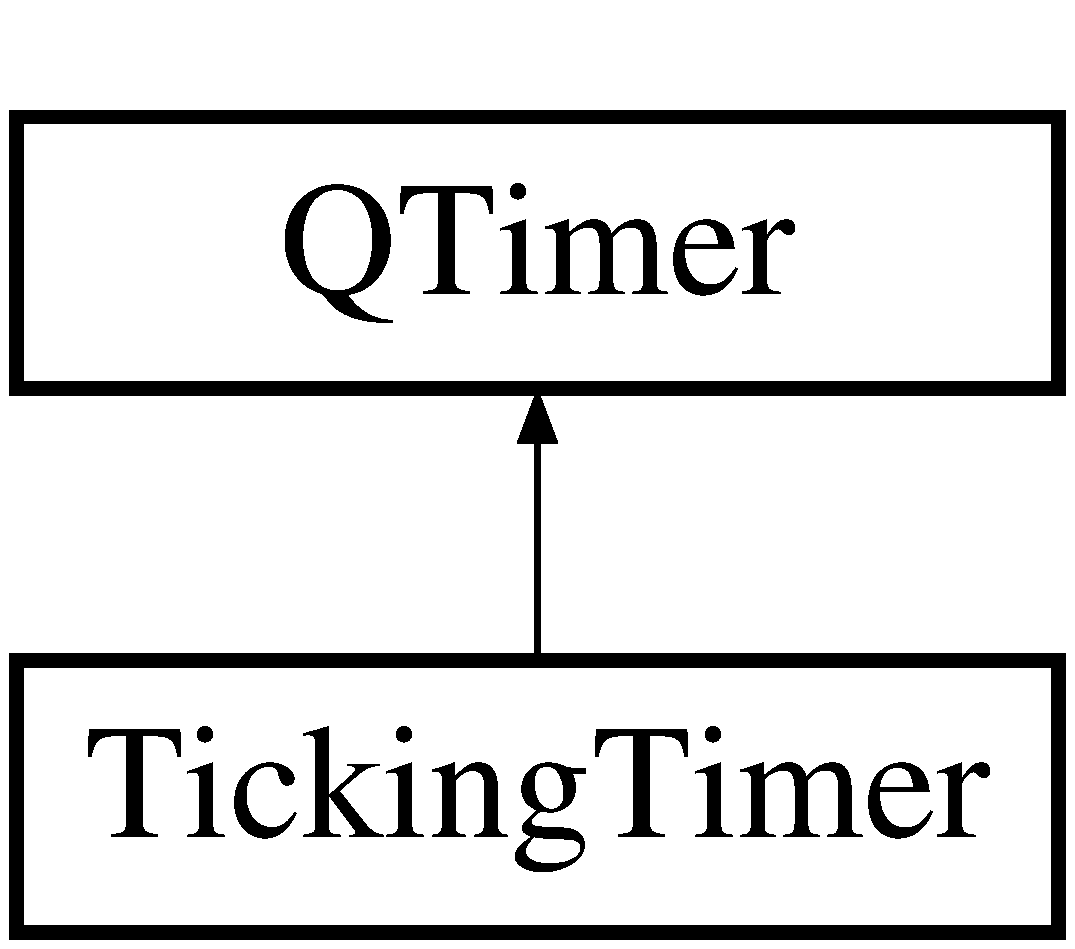
\includegraphics[height=2.000000cm]{classTickingTimer}
\end{center}
\end{figure}
\subsection*{Public Member Functions}
\begin{DoxyCompactItemize}
\item 
\hyperlink{classTickingTimer_abe9812a21ff1e231fa84041df5963a47}{Ticking\-Timer} (Q\-Object $\ast$parent=0)
\item 
void \hyperlink{classTickingTimer_a0f7c3da243271bcd1ffa833ebdc9c3a4}{start\-Ticking} (int msecs)
\item 
void \hyperlink{classTickingTimer_a7d4b5761d1fd127ab80e3249153df87b}{start\-Ticking} (int msecs, int total\-\_\-ticks)
\item 
int \hyperlink{classTickingTimer_aaddf41adb8a5dbe0346c44caf3fb0102}{get\-Ticks} () const 
\item 
int \hyperlink{classTickingTimer_a152763464d2d7be6b8a7877409ae1d24}{get\-Tick\-Limit} () const 
\end{DoxyCompactItemize}


\subsection{Constructor \& Destructor Documentation}
\hypertarget{classTickingTimer_abe9812a21ff1e231fa84041df5963a47}{\index{Ticking\-Timer@{Ticking\-Timer}!Ticking\-Timer@{Ticking\-Timer}}
\index{Ticking\-Timer@{Ticking\-Timer}!TickingTimer@{Ticking\-Timer}}
\subsubsection[{Ticking\-Timer}]{\setlength{\rightskip}{0pt plus 5cm}Ticking\-Timer\-::\-Ticking\-Timer (
\begin{DoxyParamCaption}
\item[{Q\-Object $\ast$}]{parent = {\ttfamily 0}}
\end{DoxyParamCaption}
)}}\label{classTickingTimer_abe9812a21ff1e231fa84041df5963a47}

\begin{DoxyCode}
3                                           :
4     QTimer(parent),
5     m\_tick\_limit(0)
6 \{
7     connect(\textcolor{keyword}{this}, SIGNAL(timeout()), \textcolor{keyword}{this}, SLOT(tick()));
8 \}
\end{DoxyCode}


\subsection{Member Function Documentation}
\hypertarget{classTickingTimer_a152763464d2d7be6b8a7877409ae1d24}{\index{Ticking\-Timer@{Ticking\-Timer}!get\-Tick\-Limit@{get\-Tick\-Limit}}
\index{get\-Tick\-Limit@{get\-Tick\-Limit}!TickingTimer@{Ticking\-Timer}}
\subsubsection[{get\-Tick\-Limit}]{\setlength{\rightskip}{0pt plus 5cm}int Ticking\-Timer\-::get\-Tick\-Limit (
\begin{DoxyParamCaption}
{}
\end{DoxyParamCaption}
) const}}\label{classTickingTimer_a152763464d2d7be6b8a7877409ae1d24}

\begin{DoxyCode}
28 \{
29     \textcolor{keywordflow}{return} m\_tick\_limit;
30 \}
\end{DoxyCode}
\hypertarget{classTickingTimer_aaddf41adb8a5dbe0346c44caf3fb0102}{\index{Ticking\-Timer@{Ticking\-Timer}!get\-Ticks@{get\-Ticks}}
\index{get\-Ticks@{get\-Ticks}!TickingTimer@{Ticking\-Timer}}
\subsubsection[{get\-Ticks}]{\setlength{\rightskip}{0pt plus 5cm}int Ticking\-Timer\-::get\-Ticks (
\begin{DoxyParamCaption}
{}
\end{DoxyParamCaption}
) const}}\label{classTickingTimer_aaddf41adb8a5dbe0346c44caf3fb0102}

\begin{DoxyCode}
24 \{
25     \textcolor{keywordflow}{return} m\_ticks;
26 \}
\end{DoxyCode}
\hypertarget{classTickingTimer_a0f7c3da243271bcd1ffa833ebdc9c3a4}{\index{Ticking\-Timer@{Ticking\-Timer}!start\-Ticking@{start\-Ticking}}
\index{start\-Ticking@{start\-Ticking}!TickingTimer@{Ticking\-Timer}}
\subsubsection[{start\-Ticking}]{\setlength{\rightskip}{0pt plus 5cm}void Ticking\-Timer\-::start\-Ticking (
\begin{DoxyParamCaption}
\item[{int}]{msecs}
\end{DoxyParamCaption}
)}}\label{classTickingTimer_a0f7c3da243271bcd1ffa833ebdc9c3a4}

\begin{DoxyCode}
11 \{
12     m\_ticks = 0;
13     this->start(msecs);
14 \}
\end{DoxyCode}
\hypertarget{classTickingTimer_a7d4b5761d1fd127ab80e3249153df87b}{\index{Ticking\-Timer@{Ticking\-Timer}!start\-Ticking@{start\-Ticking}}
\index{start\-Ticking@{start\-Ticking}!TickingTimer@{Ticking\-Timer}}
\subsubsection[{start\-Ticking}]{\setlength{\rightskip}{0pt plus 5cm}void Ticking\-Timer\-::start\-Ticking (
\begin{DoxyParamCaption}
\item[{int}]{msecs, }
\item[{int}]{total\-\_\-ticks}
\end{DoxyParamCaption}
)}}\label{classTickingTimer_a7d4b5761d1fd127ab80e3249153df87b}

\begin{DoxyCode}
17 \{
18     m\_ticks = 0;
19     m\_tick\_limit = total\_ticks;
20     this->start(msecs);
21 \}
\end{DoxyCode}


The documentation for this class was generated from the following files\-:\begin{DoxyCompactItemize}
\item 
Util/\hyperlink{tickingtimer_8h}{tickingtimer.\-h}\item 
Util/\hyperlink{tickingtimer_8cpp}{tickingtimer.\-cpp}\end{DoxyCompactItemize}

\hypertarget{structutf16__counter}{\section{utf16\-\_\-counter Struct Reference}
\label{structutf16__counter}\index{utf16\-\_\-counter@{utf16\-\_\-counter}}
}
\subsection*{Public Types}
\begin{DoxyCompactItemize}
\item 
typedef size\-\_\-t \hyperlink{structutf16__counter_a0d63f9ca809d182b2f184ef93bd11107}{value\-\_\-type}
\end{DoxyCompactItemize}
\subsection*{Static Public Member Functions}
\begin{DoxyCompactItemize}
\item 
static \hyperlink{structutf16__counter_a0d63f9ca809d182b2f184ef93bd11107}{value\-\_\-type} \hyperlink{structutf16__counter_a4571f3d0fbf0ce763904ec3321dcb41e}{low} (\hyperlink{structutf16__counter_a0d63f9ca809d182b2f184ef93bd11107}{value\-\_\-type} result, uint32\-\_\-t)
\item 
static \hyperlink{structutf16__counter_a0d63f9ca809d182b2f184ef93bd11107}{value\-\_\-type} \hyperlink{structutf16__counter_ac1a8793996e57dc28fd22f3165628e4d}{high} (\hyperlink{structutf16__counter_a0d63f9ca809d182b2f184ef93bd11107}{value\-\_\-type} result, uint32\-\_\-t)
\end{DoxyCompactItemize}


\subsection{Member Typedef Documentation}
\hypertarget{structutf16__counter_a0d63f9ca809d182b2f184ef93bd11107}{\index{utf16\-\_\-counter@{utf16\-\_\-counter}!value\-\_\-type@{value\-\_\-type}}
\index{value\-\_\-type@{value\-\_\-type}!utf16_counter@{utf16\-\_\-counter}}
\subsubsection[{value\-\_\-type}]{\setlength{\rightskip}{0pt plus 5cm}typedef size\-\_\-t {\bf utf16\-\_\-counter\-::value\-\_\-type}}}\label{structutf16__counter_a0d63f9ca809d182b2f184ef93bd11107}


\subsection{Member Function Documentation}
\hypertarget{structutf16__counter_ac1a8793996e57dc28fd22f3165628e4d}{\index{utf16\-\_\-counter@{utf16\-\_\-counter}!high@{high}}
\index{high@{high}!utf16_counter@{utf16\-\_\-counter}}
\subsubsection[{high}]{\setlength{\rightskip}{0pt plus 5cm}static {\bf value\-\_\-type} utf16\-\_\-counter\-::high (
\begin{DoxyParamCaption}
\item[{{\bf value\-\_\-type}}]{result, }
\item[{uint32\-\_\-t}]{}
\end{DoxyParamCaption}
)\hspace{0.3cm}{\ttfamily [inline]}, {\ttfamily [static]}}}\label{structutf16__counter_ac1a8793996e57dc28fd22f3165628e4d}

\begin{DoxyCode}
731         \{
732             \textcolor{keywordflow}{return} result + 2;
733         \}
\end{DoxyCode}
\hypertarget{structutf16__counter_a4571f3d0fbf0ce763904ec3321dcb41e}{\index{utf16\-\_\-counter@{utf16\-\_\-counter}!low@{low}}
\index{low@{low}!utf16_counter@{utf16\-\_\-counter}}
\subsubsection[{low}]{\setlength{\rightskip}{0pt plus 5cm}static {\bf value\-\_\-type} utf16\-\_\-counter\-::low (
\begin{DoxyParamCaption}
\item[{{\bf value\-\_\-type}}]{result, }
\item[{uint32\-\_\-t}]{}
\end{DoxyParamCaption}
)\hspace{0.3cm}{\ttfamily [inline]}, {\ttfamily [static]}}}\label{structutf16__counter_a4571f3d0fbf0ce763904ec3321dcb41e}

\begin{DoxyCode}
726         \{
727             \textcolor{keywordflow}{return} result + 1;
728         \}
\end{DoxyCode}


The documentation for this struct was generated from the following file\-:\begin{DoxyCompactItemize}
\item 
Third\-Party/pugixml/\hyperlink{pugixml_8cpp}{pugixml.\-cpp}\end{DoxyCompactItemize}

\hypertarget{structutf16__writer}{\section{utf16\-\_\-writer Struct Reference}
\label{structutf16__writer}\index{utf16\-\_\-writer@{utf16\-\_\-writer}}
}
\subsection*{Public Types}
\begin{DoxyCompactItemize}
\item 
typedef uint16\-\_\-t $\ast$ \hyperlink{structutf16__writer_a527b705eaf5099167b8bc42423ce918c}{value\-\_\-type}
\end{DoxyCompactItemize}
\subsection*{Static Public Member Functions}
\begin{DoxyCompactItemize}
\item 
static \hyperlink{structutf16__writer_a527b705eaf5099167b8bc42423ce918c}{value\-\_\-type} \hyperlink{structutf16__writer_ab11fef721a8b38de5e315d2e75d12956}{low} (\hyperlink{structutf16__writer_a527b705eaf5099167b8bc42423ce918c}{value\-\_\-type} result, uint32\-\_\-t ch)
\item 
static \hyperlink{structutf16__writer_a527b705eaf5099167b8bc42423ce918c}{value\-\_\-type} \hyperlink{structutf16__writer_a01b6ce1a567dea11daead3ca83f42d5c}{high} (\hyperlink{structutf16__writer_a527b705eaf5099167b8bc42423ce918c}{value\-\_\-type} result, uint32\-\_\-t ch)
\item 
static \hyperlink{structutf16__writer_a527b705eaf5099167b8bc42423ce918c}{value\-\_\-type} \hyperlink{structutf16__writer_ac14e06db126fbbef4be7efdb80fbdf4a}{any} (\hyperlink{structutf16__writer_a527b705eaf5099167b8bc42423ce918c}{value\-\_\-type} result, uint32\-\_\-t ch)
\end{DoxyCompactItemize}


\subsection{Member Typedef Documentation}
\hypertarget{structutf16__writer_a527b705eaf5099167b8bc42423ce918c}{\index{utf16\-\_\-writer@{utf16\-\_\-writer}!value\-\_\-type@{value\-\_\-type}}
\index{value\-\_\-type@{value\-\_\-type}!utf16_writer@{utf16\-\_\-writer}}
\subsubsection[{value\-\_\-type}]{\setlength{\rightskip}{0pt plus 5cm}typedef uint16\-\_\-t$\ast$ {\bf utf16\-\_\-writer\-::value\-\_\-type}}}\label{structutf16__writer_a527b705eaf5099167b8bc42423ce918c}


\subsection{Member Function Documentation}
\hypertarget{structutf16__writer_ac14e06db126fbbef4be7efdb80fbdf4a}{\index{utf16\-\_\-writer@{utf16\-\_\-writer}!any@{any}}
\index{any@{any}!utf16_writer@{utf16\-\_\-writer}}
\subsubsection[{any}]{\setlength{\rightskip}{0pt plus 5cm}static {\bf value\-\_\-type} utf16\-\_\-writer\-::any (
\begin{DoxyParamCaption}
\item[{{\bf value\-\_\-type}}]{result, }
\item[{uint32\-\_\-t}]{ch}
\end{DoxyParamCaption}
)\hspace{0.3cm}{\ttfamily [inline]}, {\ttfamily [static]}}}\label{structutf16__writer_ac14e06db126fbbef4be7efdb80fbdf4a}

\begin{DoxyCode}
759         \{
760             \textcolor{keywordflow}{return} (ch < 0x10000) ? \hyperlink{structutf16__writer_ab11fef721a8b38de5e315d2e75d12956}{low}(result, ch) : \hyperlink{structutf16__writer_a01b6ce1a567dea11daead3ca83f42d5c}{high}(result, ch);
761         \}
\end{DoxyCode}
\hypertarget{structutf16__writer_a01b6ce1a567dea11daead3ca83f42d5c}{\index{utf16\-\_\-writer@{utf16\-\_\-writer}!high@{high}}
\index{high@{high}!utf16_writer@{utf16\-\_\-writer}}
\subsubsection[{high}]{\setlength{\rightskip}{0pt plus 5cm}static {\bf value\-\_\-type} utf16\-\_\-writer\-::high (
\begin{DoxyParamCaption}
\item[{{\bf value\-\_\-type}}]{result, }
\item[{uint32\-\_\-t}]{ch}
\end{DoxyParamCaption}
)\hspace{0.3cm}{\ttfamily [inline]}, {\ttfamily [static]}}}\label{structutf16__writer_a01b6ce1a567dea11daead3ca83f42d5c}

\begin{DoxyCode}
748         \{
749             uint32\_t msh = \textcolor{keyword}{static\_cast<}uint32\_t\textcolor{keyword}{>}(ch - 0x10000) >> 10;
750             uint32\_t lsh = \textcolor{keyword}{static\_cast<}uint32\_t\textcolor{keyword}{>}(ch - 0x10000) & 0x3ff;
751 
752             result[0] = \textcolor{keyword}{static\_cast<}uint16\_t\textcolor{keyword}{>}(0xD800 + msh);
753             result[1] = \textcolor{keyword}{static\_cast<}uint16\_t\textcolor{keyword}{>}(0xDC00 + lsh);
754 
755             \textcolor{keywordflow}{return} result + 2;
756         \}
\end{DoxyCode}
\hypertarget{structutf16__writer_ab11fef721a8b38de5e315d2e75d12956}{\index{utf16\-\_\-writer@{utf16\-\_\-writer}!low@{low}}
\index{low@{low}!utf16_writer@{utf16\-\_\-writer}}
\subsubsection[{low}]{\setlength{\rightskip}{0pt plus 5cm}static {\bf value\-\_\-type} utf16\-\_\-writer\-::low (
\begin{DoxyParamCaption}
\item[{{\bf value\-\_\-type}}]{result, }
\item[{uint32\-\_\-t}]{ch}
\end{DoxyParamCaption}
)\hspace{0.3cm}{\ttfamily [inline]}, {\ttfamily [static]}}}\label{structutf16__writer_ab11fef721a8b38de5e315d2e75d12956}

\begin{DoxyCode}
741         \{
742             *result = \textcolor{keyword}{static\_cast<}uint16\_t\textcolor{keyword}{>}(ch);
743 
744             \textcolor{keywordflow}{return} result + 1;
745         \}
\end{DoxyCode}


The documentation for this struct was generated from the following file\-:\begin{DoxyCompactItemize}
\item 
Third\-Party/pugixml/\hyperlink{pugixml_8cpp}{pugixml.\-cpp}\end{DoxyCompactItemize}

\hypertarget{structutf32__counter}{\section{utf32\-\_\-counter Struct Reference}
\label{structutf32__counter}\index{utf32\-\_\-counter@{utf32\-\_\-counter}}
}
\subsection*{Public Types}
\begin{DoxyCompactItemize}
\item 
typedef size\-\_\-t \hyperlink{structutf32__counter_a6fb6728fe1a009958000f0e934fa6500}{value\-\_\-type}
\end{DoxyCompactItemize}
\subsection*{Static Public Member Functions}
\begin{DoxyCompactItemize}
\item 
static \hyperlink{structutf32__counter_a6fb6728fe1a009958000f0e934fa6500}{value\-\_\-type} \hyperlink{structutf32__counter_a3a75f4840e0391ed972ddba621d49480}{low} (\hyperlink{structutf32__counter_a6fb6728fe1a009958000f0e934fa6500}{value\-\_\-type} result, uint32\-\_\-t)
\item 
static \hyperlink{structutf32__counter_a6fb6728fe1a009958000f0e934fa6500}{value\-\_\-type} \hyperlink{structutf32__counter_aa72f5248b1dc5937330ab049bf449251}{high} (\hyperlink{structutf32__counter_a6fb6728fe1a009958000f0e934fa6500}{value\-\_\-type} result, uint32\-\_\-t)
\end{DoxyCompactItemize}


\subsection{Member Typedef Documentation}
\hypertarget{structutf32__counter_a6fb6728fe1a009958000f0e934fa6500}{\index{utf32\-\_\-counter@{utf32\-\_\-counter}!value\-\_\-type@{value\-\_\-type}}
\index{value\-\_\-type@{value\-\_\-type}!utf32_counter@{utf32\-\_\-counter}}
\subsubsection[{value\-\_\-type}]{\setlength{\rightskip}{0pt plus 5cm}typedef size\-\_\-t {\bf utf32\-\_\-counter\-::value\-\_\-type}}}\label{structutf32__counter_a6fb6728fe1a009958000f0e934fa6500}


\subsection{Member Function Documentation}
\hypertarget{structutf32__counter_aa72f5248b1dc5937330ab049bf449251}{\index{utf32\-\_\-counter@{utf32\-\_\-counter}!high@{high}}
\index{high@{high}!utf32_counter@{utf32\-\_\-counter}}
\subsubsection[{high}]{\setlength{\rightskip}{0pt plus 5cm}static {\bf value\-\_\-type} utf32\-\_\-counter\-::high (
\begin{DoxyParamCaption}
\item[{{\bf value\-\_\-type}}]{result, }
\item[{uint32\-\_\-t}]{}
\end{DoxyParamCaption}
)\hspace{0.3cm}{\ttfamily [inline]}, {\ttfamily [static]}}}\label{structutf32__counter_aa72f5248b1dc5937330ab049bf449251}

\begin{DoxyCode}
774         \{
775             \textcolor{keywordflow}{return} result + 1;
776         \}
\end{DoxyCode}
\hypertarget{structutf32__counter_a3a75f4840e0391ed972ddba621d49480}{\index{utf32\-\_\-counter@{utf32\-\_\-counter}!low@{low}}
\index{low@{low}!utf32_counter@{utf32\-\_\-counter}}
\subsubsection[{low}]{\setlength{\rightskip}{0pt plus 5cm}static {\bf value\-\_\-type} utf32\-\_\-counter\-::low (
\begin{DoxyParamCaption}
\item[{{\bf value\-\_\-type}}]{result, }
\item[{uint32\-\_\-t}]{}
\end{DoxyParamCaption}
)\hspace{0.3cm}{\ttfamily [inline]}, {\ttfamily [static]}}}\label{structutf32__counter_a3a75f4840e0391ed972ddba621d49480}

\begin{DoxyCode}
769         \{
770             \textcolor{keywordflow}{return} result + 1;
771         \}
\end{DoxyCode}


The documentation for this struct was generated from the following file\-:\begin{DoxyCompactItemize}
\item 
Third\-Party/pugixml/\hyperlink{pugixml_8cpp}{pugixml.\-cpp}\end{DoxyCompactItemize}

\hypertarget{structutf32__writer}{\section{utf32\-\_\-writer Struct Reference}
\label{structutf32__writer}\index{utf32\-\_\-writer@{utf32\-\_\-writer}}
}
\subsection*{Public Types}
\begin{DoxyCompactItemize}
\item 
typedef uint32\-\_\-t $\ast$ \hyperlink{structutf32__writer_a2284e1fa3406f113f151ded2aaa8d4ae}{value\-\_\-type}
\end{DoxyCompactItemize}
\subsection*{Static Public Member Functions}
\begin{DoxyCompactItemize}
\item 
static \hyperlink{structutf32__writer_a2284e1fa3406f113f151ded2aaa8d4ae}{value\-\_\-type} \hyperlink{structutf32__writer_a06e1b65906f7355ea54a622248095bc7}{low} (\hyperlink{structutf32__writer_a2284e1fa3406f113f151ded2aaa8d4ae}{value\-\_\-type} result, uint32\-\_\-t ch)
\item 
static \hyperlink{structutf32__writer_a2284e1fa3406f113f151ded2aaa8d4ae}{value\-\_\-type} \hyperlink{structutf32__writer_a3f86d996cde3ed7cab5c31930b67c9f1}{high} (\hyperlink{structutf32__writer_a2284e1fa3406f113f151ded2aaa8d4ae}{value\-\_\-type} result, uint32\-\_\-t ch)
\item 
static \hyperlink{structutf32__writer_a2284e1fa3406f113f151ded2aaa8d4ae}{value\-\_\-type} \hyperlink{structutf32__writer_aa94aaa4a13e755942e7da70ea7700d3e}{any} (\hyperlink{structutf32__writer_a2284e1fa3406f113f151ded2aaa8d4ae}{value\-\_\-type} result, uint32\-\_\-t ch)
\end{DoxyCompactItemize}


\subsection{Member Typedef Documentation}
\hypertarget{structutf32__writer_a2284e1fa3406f113f151ded2aaa8d4ae}{\index{utf32\-\_\-writer@{utf32\-\_\-writer}!value\-\_\-type@{value\-\_\-type}}
\index{value\-\_\-type@{value\-\_\-type}!utf32_writer@{utf32\-\_\-writer}}
\subsubsection[{value\-\_\-type}]{\setlength{\rightskip}{0pt plus 5cm}typedef uint32\-\_\-t$\ast$ {\bf utf32\-\_\-writer\-::value\-\_\-type}}}\label{structutf32__writer_a2284e1fa3406f113f151ded2aaa8d4ae}


\subsection{Member Function Documentation}
\hypertarget{structutf32__writer_aa94aaa4a13e755942e7da70ea7700d3e}{\index{utf32\-\_\-writer@{utf32\-\_\-writer}!any@{any}}
\index{any@{any}!utf32_writer@{utf32\-\_\-writer}}
\subsubsection[{any}]{\setlength{\rightskip}{0pt plus 5cm}static {\bf value\-\_\-type} utf32\-\_\-writer\-::any (
\begin{DoxyParamCaption}
\item[{{\bf value\-\_\-type}}]{result, }
\item[{uint32\-\_\-t}]{ch}
\end{DoxyParamCaption}
)\hspace{0.3cm}{\ttfamily [inline]}, {\ttfamily [static]}}}\label{structutf32__writer_aa94aaa4a13e755942e7da70ea7700d3e}

\begin{DoxyCode}
798         \{
799             *result = ch;
800 
801             \textcolor{keywordflow}{return} result + 1;
802         \}
\end{DoxyCode}
\hypertarget{structutf32__writer_a3f86d996cde3ed7cab5c31930b67c9f1}{\index{utf32\-\_\-writer@{utf32\-\_\-writer}!high@{high}}
\index{high@{high}!utf32_writer@{utf32\-\_\-writer}}
\subsubsection[{high}]{\setlength{\rightskip}{0pt plus 5cm}static {\bf value\-\_\-type} utf32\-\_\-writer\-::high (
\begin{DoxyParamCaption}
\item[{{\bf value\-\_\-type}}]{result, }
\item[{uint32\-\_\-t}]{ch}
\end{DoxyParamCaption}
)\hspace{0.3cm}{\ttfamily [inline]}, {\ttfamily [static]}}}\label{structutf32__writer_a3f86d996cde3ed7cab5c31930b67c9f1}

\begin{DoxyCode}
791         \{
792             *result = ch;
793 
794             \textcolor{keywordflow}{return} result + 1;
795         \}
\end{DoxyCode}
\hypertarget{structutf32__writer_a06e1b65906f7355ea54a622248095bc7}{\index{utf32\-\_\-writer@{utf32\-\_\-writer}!low@{low}}
\index{low@{low}!utf32_writer@{utf32\-\_\-writer}}
\subsubsection[{low}]{\setlength{\rightskip}{0pt plus 5cm}static {\bf value\-\_\-type} utf32\-\_\-writer\-::low (
\begin{DoxyParamCaption}
\item[{{\bf value\-\_\-type}}]{result, }
\item[{uint32\-\_\-t}]{ch}
\end{DoxyParamCaption}
)\hspace{0.3cm}{\ttfamily [inline]}, {\ttfamily [static]}}}\label{structutf32__writer_a06e1b65906f7355ea54a622248095bc7}

\begin{DoxyCode}
784         \{
785             *result = ch;
786 
787             \textcolor{keywordflow}{return} result + 1;
788         \}
\end{DoxyCode}


The documentation for this struct was generated from the following file\-:\begin{DoxyCompactItemize}
\item 
Third\-Party/pugixml/\hyperlink{pugixml_8cpp}{pugixml.\-cpp}\end{DoxyCompactItemize}

\hypertarget{structutf8__counter}{\section{utf8\-\_\-counter Struct Reference}
\label{structutf8__counter}\index{utf8\-\_\-counter@{utf8\-\_\-counter}}
}
\subsection*{Public Types}
\begin{DoxyCompactItemize}
\item 
typedef size\-\_\-t \hyperlink{structutf8__counter_adb65152c007965c42184614da9c4af1b}{value\-\_\-type}
\end{DoxyCompactItemize}
\subsection*{Static Public Member Functions}
\begin{DoxyCompactItemize}
\item 
static \hyperlink{structutf8__counter_adb65152c007965c42184614da9c4af1b}{value\-\_\-type} \hyperlink{structutf8__counter_a0950643189089175ae0eac9b4193534d}{low} (\hyperlink{structutf8__counter_adb65152c007965c42184614da9c4af1b}{value\-\_\-type} result, uint32\-\_\-t ch)
\item 
static \hyperlink{structutf8__counter_adb65152c007965c42184614da9c4af1b}{value\-\_\-type} \hyperlink{structutf8__counter_ab16e675980a15e1ede2e4cd18d19f7b1}{high} (\hyperlink{structutf8__counter_adb65152c007965c42184614da9c4af1b}{value\-\_\-type} result, uint32\-\_\-t)
\end{DoxyCompactItemize}


\subsection{Member Typedef Documentation}
\hypertarget{structutf8__counter_adb65152c007965c42184614da9c4af1b}{\index{utf8\-\_\-counter@{utf8\-\_\-counter}!value\-\_\-type@{value\-\_\-type}}
\index{value\-\_\-type@{value\-\_\-type}!utf8_counter@{utf8\-\_\-counter}}
\subsubsection[{value\-\_\-type}]{\setlength{\rightskip}{0pt plus 5cm}typedef size\-\_\-t {\bf utf8\-\_\-counter\-::value\-\_\-type}}}\label{structutf8__counter_adb65152c007965c42184614da9c4af1b}


\subsection{Member Function Documentation}
\hypertarget{structutf8__counter_ab16e675980a15e1ede2e4cd18d19f7b1}{\index{utf8\-\_\-counter@{utf8\-\_\-counter}!high@{high}}
\index{high@{high}!utf8_counter@{utf8\-\_\-counter}}
\subsubsection[{high}]{\setlength{\rightskip}{0pt plus 5cm}static {\bf value\-\_\-type} utf8\-\_\-counter\-::high (
\begin{DoxyParamCaption}
\item[{{\bf value\-\_\-type}}]{result, }
\item[{uint32\-\_\-t}]{}
\end{DoxyParamCaption}
)\hspace{0.3cm}{\ttfamily [inline]}, {\ttfamily [static]}}}\label{structutf8__counter_ab16e675980a15e1ede2e4cd18d19f7b1}

\begin{DoxyCode}
670         \{
671             \textcolor{comment}{// U+10000..U+10FFFF}
672             \textcolor{keywordflow}{return} result + 4;
673         \}
\end{DoxyCode}
\hypertarget{structutf8__counter_a0950643189089175ae0eac9b4193534d}{\index{utf8\-\_\-counter@{utf8\-\_\-counter}!low@{low}}
\index{low@{low}!utf8_counter@{utf8\-\_\-counter}}
\subsubsection[{low}]{\setlength{\rightskip}{0pt plus 5cm}static {\bf value\-\_\-type} utf8\-\_\-counter\-::low (
\begin{DoxyParamCaption}
\item[{{\bf value\-\_\-type}}]{result, }
\item[{uint32\-\_\-t}]{ch}
\end{DoxyParamCaption}
)\hspace{0.3cm}{\ttfamily [inline]}, {\ttfamily [static]}}}\label{structutf8__counter_a0950643189089175ae0eac9b4193534d}

\begin{DoxyCode}
660         \{
661             \textcolor{comment}{// U+0000..U+007F}
662             \textcolor{keywordflow}{if} (ch < 0x80) \textcolor{keywordflow}{return} result + 1;
663             \textcolor{comment}{// U+0080..U+07FF}
664             \textcolor{keywordflow}{else} \textcolor{keywordflow}{if} (ch < 0x800) \textcolor{keywordflow}{return} result + 2;
665             \textcolor{comment}{// U+0800..U+FFFF}
666             \textcolor{keywordflow}{else} \textcolor{keywordflow}{return} result + 3;
667         \}
\end{DoxyCode}


The documentation for this struct was generated from the following file\-:\begin{DoxyCompactItemize}
\item 
Third\-Party/pugixml/\hyperlink{pugixml_8cpp}{pugixml.\-cpp}\end{DoxyCompactItemize}

\hypertarget{structutf8__writer}{\section{utf8\-\_\-writer Struct Reference}
\label{structutf8__writer}\index{utf8\-\_\-writer@{utf8\-\_\-writer}}
}
\subsection*{Public Types}
\begin{DoxyCompactItemize}
\item 
typedef uint8\-\_\-t $\ast$ \hyperlink{structutf8__writer_af25ec3c651f9a4a3f193573a4e95002b}{value\-\_\-type}
\end{DoxyCompactItemize}
\subsection*{Static Public Member Functions}
\begin{DoxyCompactItemize}
\item 
static \hyperlink{structutf8__writer_af25ec3c651f9a4a3f193573a4e95002b}{value\-\_\-type} \hyperlink{structutf8__writer_ac4ec52da6f37225ba4fde259bff2f86c}{low} (\hyperlink{structutf8__writer_af25ec3c651f9a4a3f193573a4e95002b}{value\-\_\-type} result, uint32\-\_\-t ch)
\item 
static \hyperlink{structutf8__writer_af25ec3c651f9a4a3f193573a4e95002b}{value\-\_\-type} \hyperlink{structutf8__writer_ac03dfaf797d599afdf0be7def86ff9b9}{high} (\hyperlink{structutf8__writer_af25ec3c651f9a4a3f193573a4e95002b}{value\-\_\-type} result, uint32\-\_\-t ch)
\item 
static \hyperlink{structutf8__writer_af25ec3c651f9a4a3f193573a4e95002b}{value\-\_\-type} \hyperlink{structutf8__writer_a288e9c5f3720b95ae6b77330ad38dd56}{any} (\hyperlink{structutf8__writer_af25ec3c651f9a4a3f193573a4e95002b}{value\-\_\-type} result, uint32\-\_\-t ch)
\end{DoxyCompactItemize}


\subsection{Member Typedef Documentation}
\hypertarget{structutf8__writer_af25ec3c651f9a4a3f193573a4e95002b}{\index{utf8\-\_\-writer@{utf8\-\_\-writer}!value\-\_\-type@{value\-\_\-type}}
\index{value\-\_\-type@{value\-\_\-type}!utf8_writer@{utf8\-\_\-writer}}
\subsubsection[{value\-\_\-type}]{\setlength{\rightskip}{0pt plus 5cm}typedef uint8\-\_\-t$\ast$ {\bf utf8\-\_\-writer\-::value\-\_\-type}}}\label{structutf8__writer_af25ec3c651f9a4a3f193573a4e95002b}


\subsection{Member Function Documentation}
\hypertarget{structutf8__writer_a288e9c5f3720b95ae6b77330ad38dd56}{\index{utf8\-\_\-writer@{utf8\-\_\-writer}!any@{any}}
\index{any@{any}!utf8_writer@{utf8\-\_\-writer}}
\subsubsection[{any}]{\setlength{\rightskip}{0pt plus 5cm}static {\bf value\-\_\-type} utf8\-\_\-writer\-::any (
\begin{DoxyParamCaption}
\item[{{\bf value\-\_\-type}}]{result, }
\item[{uint32\-\_\-t}]{ch}
\end{DoxyParamCaption}
)\hspace{0.3cm}{\ttfamily [inline]}, {\ttfamily [static]}}}\label{structutf8__writer_a288e9c5f3720b95ae6b77330ad38dd56}

\begin{DoxyCode}
716         \{
717             \textcolor{keywordflow}{return} (ch < 0x10000) ? \hyperlink{structutf8__writer_ac4ec52da6f37225ba4fde259bff2f86c}{low}(result, ch) : \hyperlink{structutf8__writer_ac03dfaf797d599afdf0be7def86ff9b9}{high}(result, ch);
718         \}
\end{DoxyCode}
\hypertarget{structutf8__writer_ac03dfaf797d599afdf0be7def86ff9b9}{\index{utf8\-\_\-writer@{utf8\-\_\-writer}!high@{high}}
\index{high@{high}!utf8_writer@{utf8\-\_\-writer}}
\subsubsection[{high}]{\setlength{\rightskip}{0pt plus 5cm}static {\bf value\-\_\-type} utf8\-\_\-writer\-::high (
\begin{DoxyParamCaption}
\item[{{\bf value\-\_\-type}}]{result, }
\item[{uint32\-\_\-t}]{ch}
\end{DoxyParamCaption}
)\hspace{0.3cm}{\ttfamily [inline]}, {\ttfamily [static]}}}\label{structutf8__writer_ac03dfaf797d599afdf0be7def86ff9b9}

\begin{DoxyCode}
706         \{
707             \textcolor{comment}{// U+10000..U+10FFFF}
708             result[0] = \textcolor{keyword}{static\_cast<}uint8\_t\textcolor{keyword}{>}(0xF0 | (ch >> 18));
709             result[1] = \textcolor{keyword}{static\_cast<}uint8\_t\textcolor{keyword}{>}(0x80 | ((ch >> 12) & 0x3F));
710             result[2] = \textcolor{keyword}{static\_cast<}uint8\_t\textcolor{keyword}{>}(0x80 | ((ch >> 6) & 0x3F));
711             result[3] = \textcolor{keyword}{static\_cast<}uint8\_t\textcolor{keyword}{>}(0x80 | (ch & 0x3F));
712             \textcolor{keywordflow}{return} result + 4;
713         \}
\end{DoxyCode}
\hypertarget{structutf8__writer_ac4ec52da6f37225ba4fde259bff2f86c}{\index{utf8\-\_\-writer@{utf8\-\_\-writer}!low@{low}}
\index{low@{low}!utf8_writer@{utf8\-\_\-writer}}
\subsubsection[{low}]{\setlength{\rightskip}{0pt plus 5cm}static {\bf value\-\_\-type} utf8\-\_\-writer\-::low (
\begin{DoxyParamCaption}
\item[{{\bf value\-\_\-type}}]{result, }
\item[{uint32\-\_\-t}]{ch}
\end{DoxyParamCaption}
)\hspace{0.3cm}{\ttfamily [inline]}, {\ttfamily [static]}}}\label{structutf8__writer_ac4ec52da6f37225ba4fde259bff2f86c}

\begin{DoxyCode}
681         \{
682             \textcolor{comment}{// U+0000..U+007F}
683             \textcolor{keywordflow}{if} (ch < 0x80)
684             \{
685                 *result = \textcolor{keyword}{static\_cast<}uint8\_t\textcolor{keyword}{>}(ch);
686                 \textcolor{keywordflow}{return} result + 1;
687             \}
688             \textcolor{comment}{// U+0080..U+07FF}
689             \textcolor{keywordflow}{else} \textcolor{keywordflow}{if} (ch < 0x800)
690             \{
691                 result[0] = \textcolor{keyword}{static\_cast<}uint8\_t\textcolor{keyword}{>}(0xC0 | (ch >> 6));
692                 result[1] = \textcolor{keyword}{static\_cast<}uint8\_t\textcolor{keyword}{>}(0x80 | (ch & 0x3F));
693                 \textcolor{keywordflow}{return} result + 2;
694             \}
695             \textcolor{comment}{// U+0800..U+FFFF}
696             \textcolor{keywordflow}{else}
697             \{
698                 result[0] = \textcolor{keyword}{static\_cast<}uint8\_t\textcolor{keyword}{>}(0xE0 | (ch >> 12));
699                 result[1] = \textcolor{keyword}{static\_cast<}uint8\_t\textcolor{keyword}{>}(0x80 | ((ch >> 6) & 0x3F));
700                 result[2] = \textcolor{keyword}{static\_cast<}uint8\_t\textcolor{keyword}{>}(0x80 | (ch & 0x3F));
701                 \textcolor{keywordflow}{return} result + 3;
702             \}
703         \}
\end{DoxyCode}


The documentation for this struct was generated from the following file\-:\begin{DoxyCompactItemize}
\item 
Third\-Party/pugixml/\hyperlink{pugixml_8cpp}{pugixml.\-cpp}\end{DoxyCompactItemize}

\hypertarget{structutf__decoder}{\section{utf\-\_\-decoder$<$ Traits, opt\-\_\-swap $>$ Struct Template Reference}
\label{structutf__decoder}\index{utf\-\_\-decoder$<$ Traits, opt\-\_\-swap $>$@{utf\-\_\-decoder$<$ Traits, opt\-\_\-swap $>$}}
}
\subsection*{Static Public Member Functions}
\begin{DoxyCompactItemize}
\item 
static Traits\-::value\-\_\-type \hyperlink{structutf__decoder_a671829bbdba1eac5c8bd2bf781eae498}{decode\-\_\-utf8\-\_\-block} (const uint8\-\_\-t $\ast$data, size\-\_\-t size, typename Traits\-::value\-\_\-type result)
\item 
static Traits\-::value\-\_\-type \hyperlink{structutf__decoder_ac22afd983ac79318f0e7d07669bda8d1}{decode\-\_\-utf16\-\_\-block} (const uint16\-\_\-t $\ast$data, size\-\_\-t size, typename Traits\-::value\-\_\-type result)
\item 
static Traits\-::value\-\_\-type \hyperlink{structutf__decoder_a8bed41cc707328e8d8ab91fd7c3c943e}{decode\-\_\-utf32\-\_\-block} (const uint32\-\_\-t $\ast$data, size\-\_\-t size, typename Traits\-::value\-\_\-type result)
\item 
static Traits\-::value\-\_\-type \hyperlink{structutf__decoder_a3f728755fa7cc552e30e8d8776cad1ce}{decode\-\_\-latin1\-\_\-block} (const uint8\-\_\-t $\ast$data, size\-\_\-t size, typename Traits\-::value\-\_\-type result)
\item 
static Traits\-::value\-\_\-type \hyperlink{structutf__decoder_a56b161067860fde1ed534ac3b7399e36}{decode\-\_\-wchar\-\_\-block\-\_\-impl} (const uint16\-\_\-t $\ast$data, size\-\_\-t size, typename Traits\-::value\-\_\-type result)
\item 
static Traits\-::value\-\_\-type \hyperlink{structutf__decoder_a3bd423d3ce99b245c76be8a0796d951b}{decode\-\_\-wchar\-\_\-block\-\_\-impl} (const uint32\-\_\-t $\ast$data, size\-\_\-t size, typename Traits\-::value\-\_\-type result)
\item 
static Traits\-::value\-\_\-type \hyperlink{structutf__decoder_a5953fd0661c64408e08161342e4c538d}{decode\-\_\-wchar\-\_\-block} (const wchar\-\_\-t $\ast$data, size\-\_\-t size, typename Traits\-::value\-\_\-type result)
\end{DoxyCompactItemize}


\subsection{Member Function Documentation}
\hypertarget{structutf__decoder_a3f728755fa7cc552e30e8d8776cad1ce}{\index{utf\-\_\-decoder@{utf\-\_\-decoder}!decode\-\_\-latin1\-\_\-block@{decode\-\_\-latin1\-\_\-block}}
\index{decode\-\_\-latin1\-\_\-block@{decode\-\_\-latin1\-\_\-block}!utf_decoder@{utf\-\_\-decoder}}
\subsubsection[{decode\-\_\-latin1\-\_\-block}]{\setlength{\rightskip}{0pt plus 5cm}template$<$typename Traits , typename opt\-\_\-swap  = opt\-\_\-false$>$ static Traits\-::value\-\_\-type {\bf utf\-\_\-decoder}$<$ Traits, opt\-\_\-swap $>$\-::decode\-\_\-latin1\-\_\-block (
\begin{DoxyParamCaption}
\item[{const uint8\-\_\-t $\ast$}]{data, }
\item[{size\-\_\-t}]{size, }
\item[{typename Traits\-::value\-\_\-type}]{result}
\end{DoxyParamCaption}
)\hspace{0.3cm}{\ttfamily [inline]}, {\ttfamily [static]}}}\label{structutf__decoder_a3f728755fa7cc552e30e8d8776cad1ce}

\begin{DoxyCode}
979         \{
980             \textcolor{keywordflow}{for} (\textcolor{keywordtype}{size\_t} i = 0; i < size; ++i)
981             \{
982                 result = Traits::low(result, data[i]);
983             \}
984 
985             \textcolor{keywordflow}{return} result;
986         \}
\end{DoxyCode}
\hypertarget{structutf__decoder_ac22afd983ac79318f0e7d07669bda8d1}{\index{utf\-\_\-decoder@{utf\-\_\-decoder}!decode\-\_\-utf16\-\_\-block@{decode\-\_\-utf16\-\_\-block}}
\index{decode\-\_\-utf16\-\_\-block@{decode\-\_\-utf16\-\_\-block}!utf_decoder@{utf\-\_\-decoder}}
\subsubsection[{decode\-\_\-utf16\-\_\-block}]{\setlength{\rightskip}{0pt plus 5cm}template$<$typename Traits , typename opt\-\_\-swap  = opt\-\_\-false$>$ static Traits\-::value\-\_\-type {\bf utf\-\_\-decoder}$<$ Traits, opt\-\_\-swap $>$\-::decode\-\_\-utf16\-\_\-block (
\begin{DoxyParamCaption}
\item[{const uint16\-\_\-t $\ast$}]{data, }
\item[{size\-\_\-t}]{size, }
\item[{typename Traits\-::value\-\_\-type}]{result}
\end{DoxyParamCaption}
)\hspace{0.3cm}{\ttfamily [inline]}, {\ttfamily [static]}}}\label{structutf__decoder_ac22afd983ac79318f0e7d07669bda8d1}

\begin{DoxyCode}
910         \{
911             \textcolor{keyword}{const} uint16\_t* end = data + size;
912 
913             \textcolor{keywordflow}{while} (data < end)
914             \{
915                 uint16\_t lead = opt\_swap::value ? \hyperlink{pugixml_8cpp_a6d31b21cfa4167d79865a7797b33f3f1}{endian\_swap}(*data) : *data;
916 
917                 \textcolor{comment}{// U+0000..U+D7FF}
918                 \textcolor{keywordflow}{if} (lead < 0xD800)
919                 \{
920                     result = Traits::low(result, lead);
921                     data += 1;
922                 \}
923                 \textcolor{comment}{// U+E000..U+FFFF}
924                 \textcolor{keywordflow}{else} \textcolor{keywordflow}{if} (static\_cast<unsigned int>(lead - 0xE000) < 0x2000)
925                 \{
926                     result = Traits::low(result, lead);
927                     data += 1;
928                 \}
929                 \textcolor{comment}{// surrogate pair lead}
930                 \textcolor{keywordflow}{else} \textcolor{keywordflow}{if} (static\_cast<unsigned int>(lead - 0xD800) < 0x400 && data + 1 < end)
931                 \{
932                     uint16\_t next = opt\_swap::value ? \hyperlink{pugixml_8cpp_a6d31b21cfa4167d79865a7797b33f3f1}{endian\_swap}(data[1]) : data[1];
933 
934                     \textcolor{keywordflow}{if} (static\_cast<unsigned int>(next - 0xDC00) < 0x400)
935                     \{
936                         result = Traits::high(result, 0x10000 + ((lead & 0x3ff) << 10) + (next & 0x3ff));
937                         data += 2;
938                     \}
939                     \textcolor{keywordflow}{else}
940                     \{
941                         data += 1;
942                     \}
943                 \}
944                 \textcolor{keywordflow}{else}
945                 \{
946                     data += 1;
947                 \}
948             \}
949 
950             \textcolor{keywordflow}{return} result;
951         \}
\end{DoxyCode}
\hypertarget{structutf__decoder_a8bed41cc707328e8d8ab91fd7c3c943e}{\index{utf\-\_\-decoder@{utf\-\_\-decoder}!decode\-\_\-utf32\-\_\-block@{decode\-\_\-utf32\-\_\-block}}
\index{decode\-\_\-utf32\-\_\-block@{decode\-\_\-utf32\-\_\-block}!utf_decoder@{utf\-\_\-decoder}}
\subsubsection[{decode\-\_\-utf32\-\_\-block}]{\setlength{\rightskip}{0pt plus 5cm}template$<$typename Traits , typename opt\-\_\-swap  = opt\-\_\-false$>$ static Traits\-::value\-\_\-type {\bf utf\-\_\-decoder}$<$ Traits, opt\-\_\-swap $>$\-::decode\-\_\-utf32\-\_\-block (
\begin{DoxyParamCaption}
\item[{const uint32\-\_\-t $\ast$}]{data, }
\item[{size\-\_\-t}]{size, }
\item[{typename Traits\-::value\-\_\-type}]{result}
\end{DoxyParamCaption}
)\hspace{0.3cm}{\ttfamily [inline]}, {\ttfamily [static]}}}\label{structutf__decoder_a8bed41cc707328e8d8ab91fd7c3c943e}

\begin{DoxyCode}
954         \{
955             \textcolor{keyword}{const} uint32\_t* end = data + size;
956 
957             \textcolor{keywordflow}{while} (data < end)
958             \{
959                 uint32\_t lead = opt\_swap::value ? \hyperlink{pugixml_8cpp_a6d31b21cfa4167d79865a7797b33f3f1}{endian\_swap}(*data) : *data;
960 
961                 \textcolor{comment}{// U+0000..U+FFFF}
962                 \textcolor{keywordflow}{if} (lead < 0x10000)
963                 \{
964                     result = Traits::low(result, lead);
965                     data += 1;
966                 \}
967                 \textcolor{comment}{// U+10000..U+10FFFF}
968                 \textcolor{keywordflow}{else}
969                 \{
970                     result = Traits::high(result, lead);
971                     data += 1;
972                 \}
973             \}
974 
975             \textcolor{keywordflow}{return} result;
976         \}
\end{DoxyCode}
\hypertarget{structutf__decoder_a671829bbdba1eac5c8bd2bf781eae498}{\index{utf\-\_\-decoder@{utf\-\_\-decoder}!decode\-\_\-utf8\-\_\-block@{decode\-\_\-utf8\-\_\-block}}
\index{decode\-\_\-utf8\-\_\-block@{decode\-\_\-utf8\-\_\-block}!utf_decoder@{utf\-\_\-decoder}}
\subsubsection[{decode\-\_\-utf8\-\_\-block}]{\setlength{\rightskip}{0pt plus 5cm}template$<$typename Traits , typename opt\-\_\-swap  = opt\-\_\-false$>$ static Traits\-::value\-\_\-type {\bf utf\-\_\-decoder}$<$ Traits, opt\-\_\-swap $>$\-::decode\-\_\-utf8\-\_\-block (
\begin{DoxyParamCaption}
\item[{const uint8\-\_\-t $\ast$}]{data, }
\item[{size\-\_\-t}]{size, }
\item[{typename Traits\-::value\-\_\-type}]{result}
\end{DoxyParamCaption}
)\hspace{0.3cm}{\ttfamily [inline]}, {\ttfamily [static]}}}\label{structutf__decoder_a671829bbdba1eac5c8bd2bf781eae498}

\begin{DoxyCode}
848         \{
849             \textcolor{keyword}{const} uint8\_t utf8\_byte\_mask = 0x3f;
850 
851             \textcolor{keywordflow}{while} (size)
852             \{
853                 uint8\_t lead = *data;
854 
855                 \textcolor{comment}{// 0xxxxxxx -> U+0000..U+007F}
856                 \textcolor{keywordflow}{if} (lead < 0x80)
857                 \{
858                     result = Traits::low(result, lead);
859                     data += 1;
860                     size -= 1;
861 
862                     \textcolor{comment}{// process aligned single-byte (ascii) blocks}
863                     \textcolor{keywordflow}{if} ((reinterpret\_cast<uintptr\_t>(data) & 3) == 0)
864                     \{
865                         \textcolor{comment}{// round-trip through void* to silence 'cast increases required alignment of target
       type' warnings}
866                         \textcolor{keywordflow}{while} (size >= 4 && (*static\_cast<const uint32\_t*>(static\_cast<const void*>(data)) 
      & 0x80808080) == 0)
867                         \{
868                             result = Traits::low(result, data[0]);
869                             result = Traits::low(result, data[1]);
870                             result = Traits::low(result, data[2]);
871                             result = Traits::low(result, data[3]);
872                             data += 4;
873                             size -= 4;
874                         \}
875                     \}
876                 \}
877                 \textcolor{comment}{// 110xxxxx -> U+0080..U+07FF}
878                 \textcolor{keywordflow}{else} \textcolor{keywordflow}{if} (static\_cast<unsigned int>(lead - 0xC0) < 0x20 && size >= 2 && (data[1] & 0xc0) == 
      0x80)
879                 \{
880                     result = Traits::low(result, ((lead & ~0xC0) << 6) | (data[1] & utf8\_byte\_mask));
881                     data += 2;
882                     size -= 2;
883                 \}
884                 \textcolor{comment}{// 1110xxxx -> U+0800-U+FFFF}
885                 \textcolor{keywordflow}{else} \textcolor{keywordflow}{if} (static\_cast<unsigned int>(lead - 0xE0) < 0x10 && size >= 3 && (data[1] & 0xc0) == 
      0x80 && (data[2] & 0xc0) == 0x80)
886                 \{
887                     result = Traits::low(result, ((lead & ~0xE0) << 12) | ((data[1] & utf8\_byte\_mask) << 6)
       | (data[2] & utf8\_byte\_mask));
888                     data += 3;
889                     size -= 3;
890                 \}
891                 \textcolor{comment}{// 11110xxx -> U+10000..U+10FFFF}
892                 \textcolor{keywordflow}{else} \textcolor{keywordflow}{if} (static\_cast<unsigned int>(lead - 0xF0) < 0x08 && size >= 4 && (data[1] & 0xc0) == 
      0x80 && (data[2] & 0xc0) == 0x80 && (data[3] & 0xc0) == 0x80)
893                 \{
894                     result = Traits::high(result, ((lead & ~0xF0) << 18) | ((data[1] & utf8\_byte\_mask) << 1
      2) | ((data[2] & utf8\_byte\_mask) << 6) | (data[3] & utf8\_byte\_mask));
895                     data += 4;
896                     size -= 4;
897                 \}
898                 \textcolor{comment}{// 10xxxxxx or 11111xxx -> invalid}
899                 \textcolor{keywordflow}{else}
900                 \{
901                     data += 1;
902                     size -= 1;
903                 \}
904             \}
905 
906             \textcolor{keywordflow}{return} result;
907         \}
\end{DoxyCode}
\hypertarget{structutf__decoder_a5953fd0661c64408e08161342e4c538d}{\index{utf\-\_\-decoder@{utf\-\_\-decoder}!decode\-\_\-wchar\-\_\-block@{decode\-\_\-wchar\-\_\-block}}
\index{decode\-\_\-wchar\-\_\-block@{decode\-\_\-wchar\-\_\-block}!utf_decoder@{utf\-\_\-decoder}}
\subsubsection[{decode\-\_\-wchar\-\_\-block}]{\setlength{\rightskip}{0pt plus 5cm}template$<$typename Traits , typename opt\-\_\-swap  = opt\-\_\-false$>$ static Traits\-::value\-\_\-type {\bf utf\-\_\-decoder}$<$ Traits, opt\-\_\-swap $>$\-::decode\-\_\-wchar\-\_\-block (
\begin{DoxyParamCaption}
\item[{const wchar\-\_\-t $\ast$}]{data, }
\item[{size\-\_\-t}]{size, }
\item[{typename Traits\-::value\-\_\-type}]{result}
\end{DoxyParamCaption}
)\hspace{0.3cm}{\ttfamily [inline]}, {\ttfamily [static]}}}\label{structutf__decoder_a5953fd0661c64408e08161342e4c538d}

\begin{DoxyCode}
999         \{
1000             \textcolor{keywordflow}{return} \hyperlink{structutf__decoder_a56b161067860fde1ed534ac3b7399e36}{decode\_wchar\_block\_impl}(\textcolor{keyword}{reinterpret\_cast<}\textcolor{keyword}{const }
      \hyperlink{structwchar__selector}{wchar\_selector<sizeof(wchar\_t)>::type}*\textcolor{keyword}{>}(data), size, result);
1001         \}
\end{DoxyCode}
\hypertarget{structutf__decoder_a56b161067860fde1ed534ac3b7399e36}{\index{utf\-\_\-decoder@{utf\-\_\-decoder}!decode\-\_\-wchar\-\_\-block\-\_\-impl@{decode\-\_\-wchar\-\_\-block\-\_\-impl}}
\index{decode\-\_\-wchar\-\_\-block\-\_\-impl@{decode\-\_\-wchar\-\_\-block\-\_\-impl}!utf_decoder@{utf\-\_\-decoder}}
\subsubsection[{decode\-\_\-wchar\-\_\-block\-\_\-impl}]{\setlength{\rightskip}{0pt plus 5cm}template$<$typename Traits , typename opt\-\_\-swap  = opt\-\_\-false$>$ static Traits\-::value\-\_\-type {\bf utf\-\_\-decoder}$<$ Traits, opt\-\_\-swap $>$\-::decode\-\_\-wchar\-\_\-block\-\_\-impl (
\begin{DoxyParamCaption}
\item[{const uint16\-\_\-t $\ast$}]{data, }
\item[{size\-\_\-t}]{size, }
\item[{typename Traits\-::value\-\_\-type}]{result}
\end{DoxyParamCaption}
)\hspace{0.3cm}{\ttfamily [inline]}, {\ttfamily [static]}}}\label{structutf__decoder_a56b161067860fde1ed534ac3b7399e36}

\begin{DoxyCode}
989         \{
990             \textcolor{keywordflow}{return} \hyperlink{structutf__decoder_ac22afd983ac79318f0e7d07669bda8d1}{decode\_utf16\_block}(data, size, result);
991         \}
\end{DoxyCode}
\hypertarget{structutf__decoder_a3bd423d3ce99b245c76be8a0796d951b}{\index{utf\-\_\-decoder@{utf\-\_\-decoder}!decode\-\_\-wchar\-\_\-block\-\_\-impl@{decode\-\_\-wchar\-\_\-block\-\_\-impl}}
\index{decode\-\_\-wchar\-\_\-block\-\_\-impl@{decode\-\_\-wchar\-\_\-block\-\_\-impl}!utf_decoder@{utf\-\_\-decoder}}
\subsubsection[{decode\-\_\-wchar\-\_\-block\-\_\-impl}]{\setlength{\rightskip}{0pt plus 5cm}template$<$typename Traits , typename opt\-\_\-swap  = opt\-\_\-false$>$ static Traits\-::value\-\_\-type {\bf utf\-\_\-decoder}$<$ Traits, opt\-\_\-swap $>$\-::decode\-\_\-wchar\-\_\-block\-\_\-impl (
\begin{DoxyParamCaption}
\item[{const uint32\-\_\-t $\ast$}]{data, }
\item[{size\-\_\-t}]{size, }
\item[{typename Traits\-::value\-\_\-type}]{result}
\end{DoxyParamCaption}
)\hspace{0.3cm}{\ttfamily [inline]}, {\ttfamily [static]}}}\label{structutf__decoder_a3bd423d3ce99b245c76be8a0796d951b}

\begin{DoxyCode}
994         \{
995             \textcolor{keywordflow}{return} \hyperlink{structutf__decoder_a8bed41cc707328e8d8ab91fd7c3c943e}{decode\_utf32\_block}(data, size, result);
996         \}
\end{DoxyCode}


The documentation for this struct was generated from the following file\-:\begin{DoxyCompactItemize}
\item 
Third\-Party/pugixml/\hyperlink{pugixml_8cpp}{pugixml.\-cpp}\end{DoxyCompactItemize}

\hypertarget{classVideoControlsWidget}{\section{Video\-Controls\-Widget Class Reference}
\label{classVideoControlsWidget}\index{Video\-Controls\-Widget@{Video\-Controls\-Widget}}
}


{\ttfamily \#include $<$videocontrolswidget.\-h$>$}

Inheritance diagram for Video\-Controls\-Widget\-:\begin{figure}[H]
\begin{center}
\leavevmode
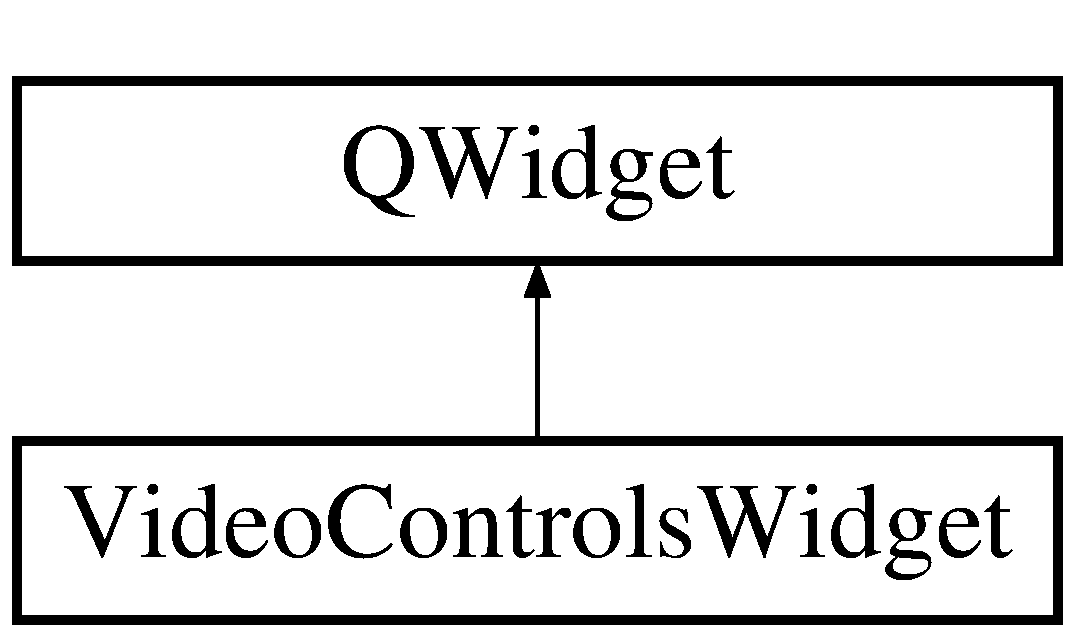
\includegraphics[height=2.000000cm]{classVideoControlsWidget}
\end{center}
\end{figure}
\subsection*{Public Slots}
\begin{DoxyCompactItemize}
\item 
void \hyperlink{classVideoControlsWidget_aff63e3d97d541cf8c05d53dd32e26292}{send\-Button\-Clicked} ()
\end{DoxyCompactItemize}
\subsection*{Signals}
\begin{DoxyCompactItemize}
\item 
void \hyperlink{classVideoControlsWidget_a5d85d6628fdb2016d49228bffb569679}{send\-Clicked} ()
\item 
void \hyperlink{classVideoControlsWidget_a9c0561d628dd239a37d1a0d52ce3a475}{send\-Clicked} (Q\-String width, Q\-String height, Q\-String fps, Q\-String bps)
\end{DoxyCompactItemize}
\subsection*{Public Member Functions}
\begin{DoxyCompactItemize}
\item 
\hyperlink{classVideoControlsWidget_ac0873fb8672cefc5f6549cac23e57757}{Video\-Controls\-Widget} (Q\-Widget $\ast$parent=0)
\item 
\hyperlink{classVideoControlsWidget_a6b85a92f3e656f11f48cdc580c2b4e0a}{$\sim$\-Video\-Controls\-Widget} ()
\item 
void \hyperlink{classVideoControlsWidget_aa7a0e5cf6d96db502d1826ec9ed43afa}{fade\-Out} ()
\item 
void \hyperlink{classVideoControlsWidget_a6fee9a987ad66923a326754e227019cc}{fade\-In} ()
\end{DoxyCompactItemize}
\subsection*{Protected Member Functions}
\begin{DoxyCompactItemize}
\item 
virtual void \hyperlink{classVideoControlsWidget_a733c88f42e0cdec6b6209c97cb2391ed}{paint\-Event} (Q\-Paint\-Event $\ast$e)
\end{DoxyCompactItemize}


\subsection{Constructor \& Destructor Documentation}
\hypertarget{classVideoControlsWidget_ac0873fb8672cefc5f6549cac23e57757}{\index{Video\-Controls\-Widget@{Video\-Controls\-Widget}!Video\-Controls\-Widget@{Video\-Controls\-Widget}}
\index{Video\-Controls\-Widget@{Video\-Controls\-Widget}!VideoControlsWidget@{Video\-Controls\-Widget}}
\subsubsection[{Video\-Controls\-Widget}]{\setlength{\rightskip}{0pt plus 5cm}Video\-Controls\-Widget\-::\-Video\-Controls\-Widget (
\begin{DoxyParamCaption}
\item[{Q\-Widget $\ast$}]{parent = {\ttfamily 0}}
\end{DoxyParamCaption}
)\hspace{0.3cm}{\ttfamily [explicit]}}}\label{classVideoControlsWidget_ac0873fb8672cefc5f6549cac23e57757}

\begin{DoxyCode}
14                                                         :
15     QWidget(parent)
16 \{
17     \textcolor{comment}{//Set up the UI}
18     this->setUpUI();
19     \textcolor{comment}{//this->fadeOut();}
20 
21     \textcolor{comment}{//setPalette(Qt::transparent);}
22     \textcolor{comment}{//setAttribute(Qt::WA\_TransparentForMouseEvents);}
23 \}
\end{DoxyCode}
\hypertarget{classVideoControlsWidget_a6b85a92f3e656f11f48cdc580c2b4e0a}{\index{Video\-Controls\-Widget@{Video\-Controls\-Widget}!$\sim$\-Video\-Controls\-Widget@{$\sim$\-Video\-Controls\-Widget}}
\index{$\sim$\-Video\-Controls\-Widget@{$\sim$\-Video\-Controls\-Widget}!VideoControlsWidget@{Video\-Controls\-Widget}}
\subsubsection[{$\sim$\-Video\-Controls\-Widget}]{\setlength{\rightskip}{0pt plus 5cm}Video\-Controls\-Widget\-::$\sim$\-Video\-Controls\-Widget (
\begin{DoxyParamCaption}
{}
\end{DoxyParamCaption}
)}}\label{classVideoControlsWidget_a6b85a92f3e656f11f48cdc580c2b4e0a}

\begin{DoxyCode}
26 \{
27     \textcolor{comment}{//DESTROY!!!!}
28 \textcolor{preprocessor}{#if !USE\_COMBO\_BOX}
29 \textcolor{preprocessor}{}    \textcolor{keyword}{delete} lblWidth;
30     \textcolor{keyword}{delete} lblHeight;
31     \textcolor{keyword}{delete} leWidth;
32     \textcolor{keyword}{delete} leHeight;
33 \textcolor{preprocessor}{#else}
34 \textcolor{preprocessor}{}    \textcolor{keyword}{delete} lblWidthHeight;
35     \textcolor{keyword}{delete} cbResolution;
36 \textcolor{preprocessor}{#endif}
37 \textcolor{preprocessor}{}    \textcolor{keyword}{delete} lblFPS;
38 
39     \textcolor{keyword}{delete} leFPS;
40     \textcolor{keyword}{delete} bSend;
41 
42 \}
\end{DoxyCode}


\subsection{Member Function Documentation}
\hypertarget{classVideoControlsWidget_a6fee9a987ad66923a326754e227019cc}{\index{Video\-Controls\-Widget@{Video\-Controls\-Widget}!fade\-In@{fade\-In}}
\index{fade\-In@{fade\-In}!VideoControlsWidget@{Video\-Controls\-Widget}}
\subsubsection[{fade\-In}]{\setlength{\rightskip}{0pt plus 5cm}void Video\-Controls\-Widget\-::fade\-In (
\begin{DoxyParamCaption}
{}
\end{DoxyParamCaption}
)}}\label{classVideoControlsWidget_a6fee9a987ad66923a326754e227019cc}

\begin{DoxyCode}
212 \{
213     this->show();
214     QGraphicsOpacityEffect *fade\_in\_effect = \textcolor{keyword}{new} QGraphicsOpacityEffect(\textcolor{keyword}{this});
215     this->setGraphicsEffect(fade\_in\_effect);
216     QPropertyAnimation *fade\_in\_animation = \textcolor{keyword}{new} QPropertyAnimation(fade\_in\_effect, \textcolor{stringliteral}{"opacity"});
217     fade\_in\_animation->setEasingCurve(QEasingCurve::InOutQuad);
218     fade\_in\_animation->setDuration(250);
219     fade\_in\_animation->setStartValue(0.1);
220     fade\_in\_animation->setEndValue(0.8);
221 
222     fade\_in\_animation->start(QPropertyAnimation::DeleteWhenStopped);
223 
224 \}
\end{DoxyCode}
\hypertarget{classVideoControlsWidget_aa7a0e5cf6d96db502d1826ec9ed43afa}{\index{Video\-Controls\-Widget@{Video\-Controls\-Widget}!fade\-Out@{fade\-Out}}
\index{fade\-Out@{fade\-Out}!VideoControlsWidget@{Video\-Controls\-Widget}}
\subsubsection[{fade\-Out}]{\setlength{\rightskip}{0pt plus 5cm}void Video\-Controls\-Widget\-::fade\-Out (
\begin{DoxyParamCaption}
{}
\end{DoxyParamCaption}
)}}\label{classVideoControlsWidget_aa7a0e5cf6d96db502d1826ec9ed43afa}

\begin{DoxyCode}
195 \{
196     QGraphicsOpacityEffect *fade\_out\_effect = \textcolor{keyword}{new} QGraphicsOpacityEffect(\textcolor{keyword}{this});
197     this->setGraphicsEffect(fade\_out\_effect);
198     QPropertyAnimation *fade\_out\_animation = \textcolor{keyword}{new} QPropertyAnimation(fade\_out\_effect, \textcolor{stringliteral}{"opacity"});
199     fade\_out\_animation->setEasingCurve(QEasingCurve::InOutQuad);
200     fade\_out\_animation->setDuration(175);
201     fade\_out\_animation->setStartValue(0.8);
202     fade\_out\_animation->setEndValue(0.0);
203 
204     fade\_out\_animation->start(QPropertyAnimation::DeleteWhenStopped);
205     \textcolor{comment}{//this->hide();}
206     QTimer::singleShot(225, \textcolor{keyword}{this}, SLOT(hideDelay()));
207 
208 \}
\end{DoxyCode}
\hypertarget{classVideoControlsWidget_a733c88f42e0cdec6b6209c97cb2391ed}{\index{Video\-Controls\-Widget@{Video\-Controls\-Widget}!paint\-Event@{paint\-Event}}
\index{paint\-Event@{paint\-Event}!VideoControlsWidget@{Video\-Controls\-Widget}}
\subsubsection[{paint\-Event}]{\setlength{\rightskip}{0pt plus 5cm}void Video\-Controls\-Widget\-::paint\-Event (
\begin{DoxyParamCaption}
\item[{Q\-Paint\-Event $\ast$}]{e}
\end{DoxyParamCaption}
)\hspace{0.3cm}{\ttfamily [protected]}, {\ttfamily [virtual]}}}\label{classVideoControlsWidget_a733c88f42e0cdec6b6209c97cb2391ed}

\begin{DoxyCode}
59 \{
60     QStyleOption opt;
61     opt.init(\textcolor{keyword}{this});
62     QPainter p(\textcolor{keyword}{this});
63     style()->drawPrimitive(QStyle::PE\_Widget, &opt, &p, \textcolor{keyword}{this});
64 \}
\end{DoxyCode}
\hypertarget{classVideoControlsWidget_aff63e3d97d541cf8c05d53dd32e26292}{\index{Video\-Controls\-Widget@{Video\-Controls\-Widget}!send\-Button\-Clicked@{send\-Button\-Clicked}}
\index{send\-Button\-Clicked@{send\-Button\-Clicked}!VideoControlsWidget@{Video\-Controls\-Widget}}
\subsubsection[{send\-Button\-Clicked}]{\setlength{\rightskip}{0pt plus 5cm}void Video\-Controls\-Widget\-::send\-Button\-Clicked (
\begin{DoxyParamCaption}
{}
\end{DoxyParamCaption}
)\hspace{0.3cm}{\ttfamily [slot]}}}\label{classVideoControlsWidget_aff63e3d97d541cf8c05d53dd32e26292}

\begin{DoxyCode}
67 \{
68     \textcolor{comment}{//emit sendClicked();}
69     \textcolor{comment}{//Determine the width field and height field}
70     QString width(\textcolor{stringliteral}{""});
71     QString height(\textcolor{stringliteral}{""});
72 \textcolor{preprocessor}{#if !USE\_COMBO\_BOX}
73 \textcolor{preprocessor}{}    width = this->leWidth->text();
74     height = this->leHeight->text()
75 \textcolor{preprocessor}{#else}
76 \textcolor{preprocessor}{}    QStringList res = this->cbResolution->currentText().split(\textcolor{stringliteral}{"x"});
77     width = res.at(0);
78     height = res.at(1);
79 \textcolor{preprocessor}{#endif}
80 \textcolor{preprocessor}{}
81     \textcolor{comment}{//Check to see if all of the fields have been filled}
82     \textcolor{keywordflow}{if}(width == \textcolor{stringliteral}{""} || height == \textcolor{stringliteral}{""} || this->leFPS->text() == \textcolor{stringliteral}{""} || this->lebitRate->text() == \textcolor{stringliteral}{""})
83     \{
84         \textcolor{comment}{//Create a message box to indicate error}
85         QMessageBox msgBox;
86         msgBox.setText(\textcolor{stringliteral}{"All fields must be filled!"});
87         \textcolor{keywordtype}{int} ret = msgBox.exec();
88 
89     \}
90     \textcolor{keywordflow}{else}
91     \{
92         \textcolor{comment}{//Inform the parent to resize the video}
93         emit \hyperlink{classVideoControlsWidget_a5d85d6628fdb2016d49228bffb569679}{sendClicked}(width, height, leFPS->text(), lebitRate->text());
94     \}
95 \}
\end{DoxyCode}
\hypertarget{classVideoControlsWidget_a5d85d6628fdb2016d49228bffb569679}{\index{Video\-Controls\-Widget@{Video\-Controls\-Widget}!send\-Clicked@{send\-Clicked}}
\index{send\-Clicked@{send\-Clicked}!VideoControlsWidget@{Video\-Controls\-Widget}}
\subsubsection[{send\-Clicked}]{\setlength{\rightskip}{0pt plus 5cm}void Video\-Controls\-Widget\-::send\-Clicked (
\begin{DoxyParamCaption}
{}
\end{DoxyParamCaption}
)\hspace{0.3cm}{\ttfamily [signal]}}}\label{classVideoControlsWidget_a5d85d6628fdb2016d49228bffb569679}
\hypertarget{classVideoControlsWidget_a9c0561d628dd239a37d1a0d52ce3a475}{\index{Video\-Controls\-Widget@{Video\-Controls\-Widget}!send\-Clicked@{send\-Clicked}}
\index{send\-Clicked@{send\-Clicked}!VideoControlsWidget@{Video\-Controls\-Widget}}
\subsubsection[{send\-Clicked}]{\setlength{\rightskip}{0pt plus 5cm}void Video\-Controls\-Widget\-::send\-Clicked (
\begin{DoxyParamCaption}
\item[{Q\-String}]{width, }
\item[{Q\-String}]{height, }
\item[{Q\-String}]{fps, }
\item[{Q\-String}]{bps}
\end{DoxyParamCaption}
)\hspace{0.3cm}{\ttfamily [signal]}}}\label{classVideoControlsWidget_a9c0561d628dd239a37d1a0d52ce3a475}


The documentation for this class was generated from the following files\-:\begin{DoxyCompactItemize}
\item 
U\-I/\hyperlink{videocontrolswidget_8h}{videocontrolswidget.\-h}\item 
U\-I/\hyperlink{videocontrolswidget_8cpp}{videocontrolswidget.\-cpp}\end{DoxyCompactItemize}

\hypertarget{classVideoWindow}{\section{Video\-Window Class Reference}
\label{classVideoWindow}\index{Video\-Window@{Video\-Window}}
}


The \hyperlink{classVideoWindow}{Video\-Window} class.  




{\ttfamily \#include $<$videowindow.\-h$>$}

Inheritance diagram for Video\-Window\-:\begin{figure}[H]
\begin{center}
\leavevmode
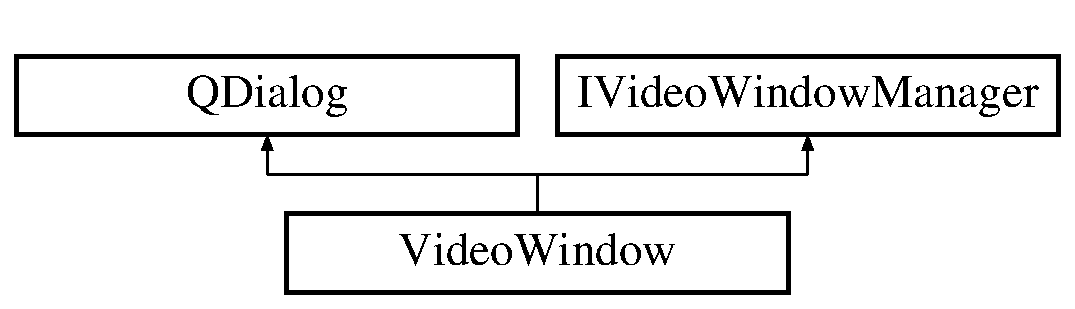
\includegraphics[height=2.000000cm]{classVideoWindow}
\end{center}
\end{figure}
\subsection*{Public Slots}
\begin{DoxyCompactItemize}
\item 
void \hyperlink{classVideoWindow_a5035f10be178cfc311d637c19938a344}{resize\-Window} (int width, int height)
\begin{DoxyCompactList}\small\item\em Slot for resizing the window. \end{DoxyCompactList}\item 
void \hyperlink{classVideoWindow_ab25ad37e9dfdb92f46212d4309d4232f}{received\-Message} (Q\-String response)
\begin{DoxyCompactList}\small\item\em A slot that will display a message in a message box. \end{DoxyCompactList}\item 
void \hyperlink{classVideoWindow_a55220de4b6b3b8e2575201c933932059}{delay\-Server\-Connect} ()
\begin{DoxyCompactList}\small\item\em A slot to connect to the server. \end{DoxyCompactList}\item 
void \hyperlink{classVideoWindow_a68b4f26c999360c30b12cc70347393c7}{disconnect} ()
\begin{DoxyCompactList}\small\item\em Slot to disconnect from the server. \end{DoxyCompactList}\item 
void \hyperlink{classVideoWindow_a655194e6449c76e200135c88f8fafd7d}{send\-Button\-Clicked} ()
\begin{DoxyCompactList}\small\item\em Slot invoked when the send button of the \hyperlink{classVideoControlsWidget}{Video\-Controls\-Widget} object is clicked. \end{DoxyCompactList}\item 
void \hyperlink{classVideoWindow_ac07f4db8a805849174cb129134708fd4}{resize\-Video} (Q\-String width, Q\-String height, Q\-String fps, Q\-String bps)
\begin{DoxyCompactList}\small\item\em Slot to send message to server to resize the video. \end{DoxyCompactList}\item 
void \hyperlink{classVideoWindow_ac8f9d111de984604f029eec9d71ced83}{on\-Bandwidth} (Q\-String bandwidth)
\begin{DoxyCompactList}\small\item\em A slot invoked when the bandwidth has changed. \end{DoxyCompactList}\end{DoxyCompactItemize}
\subsection*{Signals}
\begin{DoxyCompactItemize}
\item 
void \hyperlink{classVideoWindow_a726415adc7cbeb8ed1ac0892929ecfaf}{send\-Camera} (\hyperlink{classCamera}{Camera} $\ast$)
\begin{DoxyCompactList}\small\item\em This signal is invoked when the window is destroyed in order to inform subscribers which camera was associated with this window. \end{DoxyCompactList}\end{DoxyCompactItemize}
\subsection*{Public Member Functions}
\begin{DoxyCompactItemize}
\item 
\hyperlink{classVideoWindow_a1230a803d626de946e9fa67ebcafe1c2}{Video\-Window} (\hyperlink{classCamera}{Camera} $\ast$\hyperlink{classVideoWindow_aa163a5850ff726c12f59562b993e4403}{camera}, \hyperlink{classIControlCenterManager}{I\-Control\-Center\-Manager} $\ast$control\-\_\-center=0, Q\-Widget $\ast$parent=0)
\begin{DoxyCompactList}\small\item\em Explicit value constructor. \end{DoxyCompactList}\item 
\hyperlink{classVideoWindow_a3c5b83ed86071f9210388f0e06ac4876}{$\sim$\-Video\-Window} ()
\item 
void \hyperlink{classVideoWindow_ac71a3e790d6956a26369294d5fb36c93}{stream\-Video} (Q\-String url)
\item 
void \hyperlink{classVideoWindow_af5830c7faa6e46a69be02c93abc28d3a}{send\-Request} (Q\-String data)
\begin{DoxyCompactList}\small\item\em Send a request. \end{DoxyCompactList}\item 
\hyperlink{classCamera}{Camera} $\ast$ \hyperlink{classVideoWindow_aa163a5850ff726c12f59562b993e4403}{camera} () const 
\begin{DoxyCompactList}\small\item\em Getter for the camera object. \end{DoxyCompactList}\item 
void \hyperlink{classVideoWindow_a612b1b179b04ccebce717ff2fd95879e}{set\-Camera} (\hyperlink{classCamera}{Camera} $\ast$\hyperlink{classVideoWindow_aa163a5850ff726c12f59562b993e4403}{camera})
\begin{DoxyCompactList}\small\item\em The camera setter. \end{DoxyCompactList}\item 
bool \hyperlink{classVideoWindow_af11854a41b4e79c396c04bc40789b46d}{operator==} (const \hyperlink{classVideoWindow}{Video\-Window} \&rhs)
\begin{DoxyCompactList}\small\item\em Overloaded equivalence operator. \end{DoxyCompactList}\item 
virtual Q\-String\-List \hyperlink{classVideoWindow_a194af961938fb7a0482932dc6787ec6f}{get\-Video\-Sizes} ()
\begin{DoxyCompactList}\small\item\em Get the list of video sizes from the combo box. \end{DoxyCompactList}\end{DoxyCompactItemize}
\subsection*{Protected Member Functions}
\begin{DoxyCompactItemize}
\item 
virtual void \hyperlink{classVideoWindow_aba663642b1a2911fc83c366c50fc1378}{enter\-Event} (Q\-Event $\ast$e)
\item 
virtual void \hyperlink{classVideoWindow_a58ad769fa96f197fd1212a9cbf5984d1}{leave\-Event} (Q\-Event $\ast$e)
\end{DoxyCompactItemize}


\subsection{Detailed Description}
The \hyperlink{classVideoWindow}{Video\-Window} class. 

A window that contains the media player and media controls for a particular camera or stremaing server. 

\subsection{Constructor \& Destructor Documentation}
\hypertarget{classVideoWindow_a1230a803d626de946e9fa67ebcafe1c2}{\index{Video\-Window@{Video\-Window}!Video\-Window@{Video\-Window}}
\index{Video\-Window@{Video\-Window}!VideoWindow@{Video\-Window}}
\subsubsection[{Video\-Window}]{\setlength{\rightskip}{0pt plus 5cm}Video\-Window\-::\-Video\-Window (
\begin{DoxyParamCaption}
\item[{{\bf Camera} $\ast$}]{camera, }
\item[{{\bf I\-Control\-Center\-Manager} $\ast$}]{control\-\_\-center = {\ttfamily 0}, }
\item[{Q\-Widget $\ast$}]{parent = {\ttfamily 0}}
\end{DoxyParamCaption}
)\hspace{0.3cm}{\ttfamily [explicit]}}}\label{classVideoWindow_a1230a803d626de946e9fa67ebcafe1c2}


Explicit value constructor. 


\begin{DoxyParams}{Parameters}
{\em camera} & The camera or streaming server whose video this window will play. \\
\hline
{\em parent} & The parent widget of the window. \\
\hline
\end{DoxyParams}

\begin{DoxyCode}
10                                                                                                :
11     QDialog(parent),
12     m\_control\_center\_manager(control\_center),
13     m\_camera(camera),
14     ui(\textcolor{keyword}{new} Ui::VideoWindow),
15     m\_controls\_revealed(\textcolor{keyword}{false}),
16     m\_is\_inside(\textcolor{keyword}{false}),
17     m\_currentbw\_kbps(5000),
18     m\_decision\_interface(\textcolor{keyword}{this}),
19     m\_current\_params(),
20     m\_pending\_parameters()
21 \{   
22 
23     ui->setupUi(\textcolor{keyword}{this});
24     this->setWindowTitle(m\_camera->\hyperlink{classCamera_a5763757e8d6adb6437dde2502072a3b1}{name}());
25     \textcolor{comment}{//this->setFixedSize(this->size());}
26     this->setFixedSize(ui->video\_player->width() + 10, ui->video\_player->height() + ui->video\_controls->
      height() + 5);
27 
28     connect(ui->video\_player, SIGNAL(resizeParent(\textcolor{keywordtype}{int},\textcolor{keywordtype}{int})), \textcolor{keyword}{this}, SLOT(
      \hyperlink{classVideoWindow_a5035f10be178cfc311d637c19938a344}{resizeWindow}(\textcolor{keywordtype}{int},\textcolor{keywordtype}{int})));
29     connect(ui->video\_controls, SIGNAL(sendClicked()), \textcolor{keyword}{this}, SLOT(
      \hyperlink{classVideoWindow_a655194e6449c76e200135c88f8fafd7d}{sendButtonClicked}()));
30     connect(ui->video\_controls, SIGNAL(sendClicked(QString,QString,QString, QString)), \textcolor{keyword}{this}, SLOT(
      \hyperlink{classVideoWindow_ac07f4db8a805849174cb129134708fd4}{resizeVideo}(QString,QString,QString, QString)));
31 
32     ui->video\_controls->resize(this->width(), ui->video\_controls->height());
33     ui->video\_controls->move((this->width() / 2) - (ui->video\_controls->width() / 2),0);
34 
35     ui->video\_player->move((this->width() / 2) - (ui->video\_player->width() / 2),ui->video\_controls->height
      ());
36 
37     \textcolor{comment}{//Try to connect to server}
38     m\_tcp\_interface = \textcolor{keyword}{new} \hyperlink{classNetworkToQtInterface}{NetworkToQtInterface}(m\_camera->
      \hyperlink{classCamera_aa93654bec9b65adfb95e192ac9c71e80}{server\_address}());
39     connect(m\_tcp\_interface, SIGNAL(messageDispatch(QString)), \textcolor{keyword}{this}, SLOT(
      \hyperlink{classVideoWindow_ab25ad37e9dfdb92f46212d4309d4232f}{receivedMessage}(QString)));
40     connect(m\_tcp\_interface, SIGNAL(serverDisconnected()), \textcolor{keyword}{this}, SLOT(\hyperlink{classVideoWindow_a68b4f26c999360c30b12cc70347393c7}{disconnect}()));
41     \textcolor{comment}{//connect(m\_request\_thread, SIGNAL(destroyed()), m\_tcp\_interface, SLOT(close()));}
42 
43     this->setUpThreads();
44     \textcolor{comment}{//Delay server connect}
45 \textcolor{preprocessor}{#ifdef Q\_OS\_LINUX}
46 \textcolor{preprocessor}{}    QTimer::singleShot(500, \textcolor{keyword}{this}, SLOT(\hyperlink{classVideoWindow_a55220de4b6b3b8e2575201c933932059}{delayServerConnect}()));
47 \textcolor{preprocessor}{#endif}
48 \textcolor{preprocessor}{}
49 
50 
51     \textcolor{comment}{//qApp->installEventFilter(this);}
52 \}
\end{DoxyCode}
\hypertarget{classVideoWindow_a3c5b83ed86071f9210388f0e06ac4876}{\index{Video\-Window@{Video\-Window}!$\sim$\-Video\-Window@{$\sim$\-Video\-Window}}
\index{$\sim$\-Video\-Window@{$\sim$\-Video\-Window}!VideoWindow@{Video\-Window}}
\subsubsection[{$\sim$\-Video\-Window}]{\setlength{\rightskip}{0pt plus 5cm}Video\-Window\-::$\sim$\-Video\-Window (
\begin{DoxyParamCaption}
{}
\end{DoxyParamCaption}
)}}\label{classVideoWindow_a3c5b83ed86071f9210388f0e06ac4876}

\begin{DoxyCode}
102 \{
103     \textcolor{keyword}{delete} ui;
104     \hyperlink{Log_8h_a7cec51f4ce4b22e8c0f256485d57fca7}{INFO}() << \textcolor{stringliteral}{"Video window destructor called."};
105     \textcolor{comment}{//Must determine why server is not seeing us disconnect}
106     this->\hyperlink{classVideoWindow_a68b4f26c999360c30b12cc70347393c7}{disconnect}();
107     \textcolor{comment}{//ui->video\_player->stopPlaying();}
108 
109 
110     m\_request\_thread->terminate();
111 
112 
113     \textcolor{keyword}{delete} m\_tcp\_interface;
114 
115     \textcolor{keyword}{delete} m\_request\_thread;
116 
117     m\_bwfilereader->\hyperlink{classBandwidthFileReader_a0301d713d44225001bd87e7f423bd753}{setReadyFlag}(\textcolor{keyword}{false});
118 
119     m\_bwreaderthread->terminate();
120 
121     \textcolor{keyword}{delete} m\_bwfilereader;
122     \textcolor{keyword}{delete} m\_bwreaderthread;
123 
124     \textcolor{comment}{//Camera object should be managed by creating class}
125     \textcolor{comment}{//delete m\_camera;}
126     emit \hyperlink{classVideoWindow_a726415adc7cbeb8ed1ac0892929ecfaf}{sendCamera}(m\_camera);
127 
128 
129 
130 \}
\end{DoxyCode}


\subsection{Member Function Documentation}
\hypertarget{classVideoWindow_aa163a5850ff726c12f59562b993e4403}{\index{Video\-Window@{Video\-Window}!camera@{camera}}
\index{camera@{camera}!VideoWindow@{Video\-Window}}
\subsubsection[{camera}]{\setlength{\rightskip}{0pt plus 5cm}{\bf Camera} $\ast$ Video\-Window\-::camera (
\begin{DoxyParamCaption}
{}
\end{DoxyParamCaption}
) const}}\label{classVideoWindow_aa163a5850ff726c12f59562b993e4403}


Getter for the camera object. 

\begin{DoxyReturn}{Returns}
The camera this video window streams from. 
\end{DoxyReturn}

\begin{DoxyCode}
282 \{
283     \textcolor{keywordflow}{return} m\_camera;
284 \}
\end{DoxyCode}
\hypertarget{classVideoWindow_a55220de4b6b3b8e2575201c933932059}{\index{Video\-Window@{Video\-Window}!delay\-Server\-Connect@{delay\-Server\-Connect}}
\index{delay\-Server\-Connect@{delay\-Server\-Connect}!VideoWindow@{Video\-Window}}
\subsubsection[{delay\-Server\-Connect}]{\setlength{\rightskip}{0pt plus 5cm}void Video\-Window\-::delay\-Server\-Connect (
\begin{DoxyParamCaption}
{}
\end{DoxyParamCaption}
)\hspace{0.3cm}{\ttfamily [slot]}}}\label{classVideoWindow_a55220de4b6b3b8e2575201c933932059}


A slot to connect to the server. 

This slot is subscribed to by timers in order to delay connecting to the server specified by the camera object. The connection is delayed so that the user interface may load before blocking while attempting to connect. 
\begin{DoxyCode}
198 \{
199     connectToServer();
200 \}
\end{DoxyCode}
\hypertarget{classVideoWindow_a68b4f26c999360c30b12cc70347393c7}{\index{Video\-Window@{Video\-Window}!disconnect@{disconnect}}
\index{disconnect@{disconnect}!VideoWindow@{Video\-Window}}
\subsubsection[{disconnect}]{\setlength{\rightskip}{0pt plus 5cm}void Video\-Window\-::disconnect (
\begin{DoxyParamCaption}
{}
\end{DoxyParamCaption}
)\hspace{0.3cm}{\ttfamily [slot]}}}\label{classVideoWindow_a68b4f26c999360c30b12cc70347393c7}


Slot to disconnect from the server. 


\begin{DoxyCode}
302 \{
303     m\_tcp\_interface->\hyperlink{classNetworkToQtInterface_ac4889eb9f3c5b5e4509252481335200f}{close}();
304     
305 \}
\end{DoxyCode}
\hypertarget{classVideoWindow_aba663642b1a2911fc83c366c50fc1378}{\index{Video\-Window@{Video\-Window}!enter\-Event@{enter\-Event}}
\index{enter\-Event@{enter\-Event}!VideoWindow@{Video\-Window}}
\subsubsection[{enter\-Event}]{\setlength{\rightskip}{0pt plus 5cm}void Video\-Window\-::enter\-Event (
\begin{DoxyParamCaption}
\item[{Q\-Event $\ast$}]{e}
\end{DoxyParamCaption}
)\hspace{0.3cm}{\ttfamily [protected]}, {\ttfamily [virtual]}}}\label{classVideoWindow_aba663642b1a2911fc83c366c50fc1378}

\begin{DoxyCode}
141 \{
142 \textcolor{comment}{//    QDialog::enterEvent(e);}
143 \textcolor{comment}{//    m\_is\_inside = true;}
144 \}
\end{DoxyCode}
\hypertarget{classVideoWindow_a194af961938fb7a0482932dc6787ec6f}{\index{Video\-Window@{Video\-Window}!get\-Video\-Sizes@{get\-Video\-Sizes}}
\index{get\-Video\-Sizes@{get\-Video\-Sizes}!VideoWindow@{Video\-Window}}
\subsubsection[{get\-Video\-Sizes}]{\setlength{\rightskip}{0pt plus 5cm}Q\-String\-List Video\-Window\-::get\-Video\-Sizes (
\begin{DoxyParamCaption}
{}
\end{DoxyParamCaption}
)\hspace{0.3cm}{\ttfamily [virtual]}}}\label{classVideoWindow_a194af961938fb7a0482932dc6787ec6f}


Get the list of video sizes from the combo box. 

\begin{DoxyReturn}{Returns}
The video size list. 
\end{DoxyReturn}


Implements \hyperlink{classIVideoWindowManager_a40fe14abdb6a7ffba05841ac9be08179}{I\-Video\-Window\-Manager}.


\begin{DoxyCode}
297 \{
298     \textcolor{keywordflow}{return} this->ui->video\_controls->getSizes();
299 \}
\end{DoxyCode}
\hypertarget{classVideoWindow_a58ad769fa96f197fd1212a9cbf5984d1}{\index{Video\-Window@{Video\-Window}!leave\-Event@{leave\-Event}}
\index{leave\-Event@{leave\-Event}!VideoWindow@{Video\-Window}}
\subsubsection[{leave\-Event}]{\setlength{\rightskip}{0pt plus 5cm}void Video\-Window\-::leave\-Event (
\begin{DoxyParamCaption}
\item[{Q\-Event $\ast$}]{e}
\end{DoxyParamCaption}
)\hspace{0.3cm}{\ttfamily [protected]}, {\ttfamily [virtual]}}}\label{classVideoWindow_a58ad769fa96f197fd1212a9cbf5984d1}

\begin{DoxyCode}
147 \{
148 \textcolor{comment}{//    QDialog::leaveEvent(e);}
149 \textcolor{comment}{//    m\_is\_inside = false;}
150 \textcolor{comment}{//    //Make sure we hide the controls if revealed}
151 \textcolor{comment}{//    if(m\_controls\_revealed)}
152 \textcolor{comment}{//    \{}
153 \textcolor{comment}{//        ui->video\_controls->fadeOut();}
154 \textcolor{comment}{//        m\_controls\_revealed = false;}
155 \textcolor{comment}{//    \}}
156 \}
\end{DoxyCode}
\hypertarget{classVideoWindow_ac8f9d111de984604f029eec9d71ced83}{\index{Video\-Window@{Video\-Window}!on\-Bandwidth@{on\-Bandwidth}}
\index{on\-Bandwidth@{on\-Bandwidth}!VideoWindow@{Video\-Window}}
\subsubsection[{on\-Bandwidth}]{\setlength{\rightskip}{0pt plus 5cm}void Video\-Window\-::on\-Bandwidth (
\begin{DoxyParamCaption}
\item[{Q\-String}]{bandwidth}
\end{DoxyParamCaption}
)\hspace{0.3cm}{\ttfamily [slot]}}}\label{classVideoWindow_ac8f9d111de984604f029eec9d71ced83}


A slot invoked when the bandwidth has changed. 


\begin{DoxyParams}{Parameters}
{\em bandwidth} & The new bandwidth. \\
\hline
\end{DoxyParams}

\begin{DoxyCode}
351 \{
352     \textcolor{keywordtype}{bool} success = \textcolor{keyword}{false};
353 
354     \textcolor{keywordtype}{int} iBW = bandwidth.toInt(&success, 10);
355 
356     \textcolor{keywordflow}{if}(success)
357     \{
358         \textcolor{keywordtype}{int} oldbw = m\_currentbw\_kbps;
359         this->m\_currentbw\_kbps = iBW;
360 
361         \textcolor{comment}{//Are we in learning mode?}
362         \textcolor{keywordflow}{if}(m\_control\_center\_manager->\hyperlink{classIControlCenterManager_ab4f6172f09c27b73254ed7fcfe716790}{inLearningMode}())
363         \{
364             \textcolor{comment}{//Add training example to training set and determine the decision function}
365 
366             \textcolor{comment}{//Create the feature set object}
367             \hyperlink{classFeatureSet}{FeatureSet} next\_fs(oldbw * 1000, (\textcolor{keywordtype}{int})this->m\_camera->
      \hyperlink{classCamera_aafe2614c711fb5465dacaeea55e12f64}{content\_type}());
368             \textcolor{comment}{//Get the labels}
369 
370             \textcolor{comment}{//We use simple implicit feedback to determine the two classes.}
371 
372             \textcolor{comment}{//If the video is playing at framerate 15fps and enhanced bitrate, the user prefers bitrate
       over framerate (+1 class)}
373             \textcolor{comment}{//If the video is playing at framerate 30fps and lower bitrate, the user prefers temporal
       quality over bitrate (-1 class)}
374             \textcolor{keywordtype}{double} lbl\_fps\_bitrate = 0.0;
375             \textcolor{keywordflow}{if}(ui->video\_player->getFps() < 30)
376             \{
377                 lbl\_fps\_bitrate = 1.0;
378             \}
379             \textcolor{keywordflow}{else}
380             \{
381                 lbl\_fps\_bitrate = -1.0;
382             \}
383 
384             \textcolor{comment}{//To determine the label for size over quality, we have to look at available bandwidth and the
       bandwidth of}
385             \textcolor{comment}{//the video. If there is a significant enough difference between the available bandwidth and
       the data rate of}
386             \textcolor{comment}{//the video the user most likely prefers quality to size. In order to confirm this we will look
       at the dimensions of}
387             \textcolor{comment}{//the video and check if the current encoding bitrate constitutes high quality video. This will
       be defined as the +1}
388             \textcolor{comment}{//class. If the data rate is at the maximum that the bandwidth will allow, we will look at the
       video size, and if the}
389             \textcolor{comment}{//dimensions are large enough, then the user most likely prefers size over video quality. This
       will be defined as the -1}
390             \textcolor{comment}{//class.}
391             \textcolor{keywordtype}{double} lbl\_size\_quality = 0.0;
392             \textcolor{comment}{//For now, a trivial solution; will determine using empricial evidence}
393             \textcolor{keywordflow}{if}((\textcolor{keywordtype}{float})m\_current\_params.\hyperlink{classEncodingParameters_aefccfdee4e2f60522637066501b0258c}{bitrateAsInt}() > (float)ui->video\_player->width() * ui->
      video\_player->height() * 1.75)
394             \{
395                 \textcolor{comment}{//Preference to quality}
396                 lbl\_size\_quality = 1.0;
397             \}
398             \textcolor{keywordflow}{else}
399             \{
400                 lbl\_size\_quality = -1.0;
401             \}
402 
403             \textcolor{comment}{//Add this new training example}
404             this->m\_control\_center\_manager->\hyperlink{classIControlCenterManager_ad223b7089a7196da4edbb70adc2d333e}{addTrainingExample}(next\_fs, lbl\_fps\_bitrate, 
      lbl\_size\_quality);
405 
406         \}
407         \textcolor{keywordflow}{else}
408         \{
409             \textcolor{comment}{//Determine the new encoding parameters}
410             \hyperlink{classEncodingParameters}{EncodingParameters} new\_params;
411             \textcolor{keywordtype}{float} dr\_avg\_kbps = ui->video\_player->getAverageBitrate() * 10000;
412             \hyperlink{classFeatureSet}{FeatureSet} fs;
413             m\_decision\_interface.\hyperlink{classDecisionInterface_afd67dc2e1710da83987ad842d6b0a69a}{makeDecision}(m\_currentbw\_kbps, dr\_avg\_kbps, m\_current\_params, 
      fs, new\_params);
414 
415             this->\hyperlink{classVideoWindow_ac07f4db8a805849174cb129134708fd4}{resizeVideo}(new\_params.\hyperlink{classEncodingParameters_ad784bc5e0a14e537f1bef3340a5a816f}{width}(), new\_params.
      \hyperlink{classEncodingParameters_a65eeab477e176c521ad2aab0e46606b6}{height}(), new\_params.\hyperlink{classEncodingParameters_aaae058a54aa6b2381047170d199a5131}{fps}(), new\_params.\hyperlink{classEncodingParameters_a62e5d236efaa9594bd8706d9b6e79ba3}{bitrate}());
416 
417         \}
418     \}
419 \}
\end{DoxyCode}
\hypertarget{classVideoWindow_af11854a41b4e79c396c04bc40789b46d}{\index{Video\-Window@{Video\-Window}!operator==@{operator==}}
\index{operator==@{operator==}!VideoWindow@{Video\-Window}}
\subsubsection[{operator==}]{\setlength{\rightskip}{0pt plus 5cm}bool Video\-Window\-::operator== (
\begin{DoxyParamCaption}
\item[{const {\bf Video\-Window} \&}]{rhs}
\end{DoxyParamCaption}
)}}\label{classVideoWindow_af11854a41b4e79c396c04bc40789b46d}


Overloaded equivalence operator. 

Tests to see if two video windows are streaming from the same camera. 
\begin{DoxyParams}{Parameters}
{\em rhs} & The camera to test against. \\
\hline
\end{DoxyParams}
\begin{DoxyReturn}{Returns}
True if the two cameras are the same, false otherwise. 
\end{DoxyReturn}

\begin{DoxyCode}
292 \{
293     \textcolor{keywordflow}{return} *(this->\hyperlink{classVideoWindow_aa163a5850ff726c12f59562b993e4403}{camera}()) == *(rhs.\hyperlink{classVideoWindow_aa163a5850ff726c12f59562b993e4403}{camera}());
294 \}
\end{DoxyCode}
\hypertarget{classVideoWindow_ab25ad37e9dfdb92f46212d4309d4232f}{\index{Video\-Window@{Video\-Window}!received\-Message@{received\-Message}}
\index{received\-Message@{received\-Message}!VideoWindow@{Video\-Window}}
\subsubsection[{received\-Message}]{\setlength{\rightskip}{0pt plus 5cm}void Video\-Window\-::received\-Message (
\begin{DoxyParamCaption}
\item[{Q\-String}]{response}
\end{DoxyParamCaption}
)\hspace{0.3cm}{\ttfamily [slot]}}}\label{classVideoWindow_ab25ad37e9dfdb92f46212d4309d4232f}


A slot that will display a message in a message box. 

This slot will launch a message box with the response parameter as the displayed message. 
\begin{DoxyParams}{Parameters}
{\em response} & The message to display in a message box. \\
\hline
\end{DoxyParams}

\begin{DoxyCode}
171 \{
172     \hyperlink{Log_8h_a7cec51f4ce4b22e8c0f256485d57fca7}{INFO}() << \textcolor{stringliteral}{"In slot \(\backslash\)'receivedPacket\(\backslash\)' Message:"} << response;
173     \textcolor{comment}{//Set non modal and allocate on heap so it does not block}
174     \textcolor{comment}{//video from playing}
175     QMessageBox *msgBox = \textcolor{keyword}{new} QMessageBox;
176     msgBox->setWindowTitle(\textcolor{stringliteral}{"Server says..."});
177     msgBox->setText(response);
178     msgBox->setWindowModality(Qt::NonModal);
179     msgBox->setAttribute(Qt::WA\_DeleteOnClose);
180     msgBox->show();
181 
182     \textcolor{comment}{//Check if the response is an acceptance of the parameters}
183     \textcolor{keywordflow}{if}(response.contains(\textcolor{stringliteral}{"Updating"}))
184     \{
185         m\_current\_params = m\_pending\_parameters;
186 
187         ui->video\_player->resetStats();
188 
189         \textcolor{comment}{//If we are in learning mode}
190         \textcolor{keywordflow}{if}(m\_control\_center\_manager->\hyperlink{classIControlCenterManager_ab4f6172f09c27b73254ed7fcfe716790}{inLearningMode}())
191         \{
192             \textcolor{comment}{//Add this to the training set}
193         \}
194     \}
195 \}
\end{DoxyCode}
\hypertarget{classVideoWindow_ac07f4db8a805849174cb129134708fd4}{\index{Video\-Window@{Video\-Window}!resize\-Video@{resize\-Video}}
\index{resize\-Video@{resize\-Video}!VideoWindow@{Video\-Window}}
\subsubsection[{resize\-Video}]{\setlength{\rightskip}{0pt plus 5cm}void Video\-Window\-::resize\-Video (
\begin{DoxyParamCaption}
\item[{Q\-String}]{width, }
\item[{Q\-String}]{height, }
\item[{Q\-String}]{fps, }
\item[{Q\-String}]{bps}
\end{DoxyParamCaption}
)\hspace{0.3cm}{\ttfamily [slot]}}}\label{classVideoWindow_ac07f4db8a805849174cb129134708fd4}


Slot to send message to server to resize the video. 


\begin{DoxyCode}
319 \{
320     \textcolor{comment}{//Create the message}
321     QString msg = QString(\textcolor{stringliteral}{"start "});
322     msg += width + QString(\textcolor{stringliteral}{" "}) + height + QString(\textcolor{stringliteral}{" "}) + fps + QString(\textcolor{stringliteral}{" "}) + bps;
323     \hyperlink{Log_8h_a7cec51f4ce4b22e8c0f256485d57fca7}{INFO}() << \textcolor{stringliteral}{"Sent: "} << msg;
324     \textcolor{comment}{//Send it to server}
325     this->\hyperlink{classVideoWindow_af5830c7faa6e46a69be02c93abc28d3a}{sendRequest}(msg);
326 
327 
328 \textcolor{preprocessor}{#if PLAY\_WITH\_VLC}
329 \textcolor{preprocessor}{}    \textcolor{keywordtype}{int} fps\_int = fps.toInt();
330     \textcolor{comment}{//If FPS has changed we need to restart playback (limit to 15 and 30 fps for now... very poor and hacky
       method)}
331     \textcolor{keywordflow}{if}(fps\_int != ui->video\_player->getFps() && (fps\_int == 30 || fps\_int == 15))
332     \{
333         ui->video\_player->setFps(fps\_int);
334         \textcolor{comment}{//ui->video\_player->setPlaybackRate(fps.toInt());}
335         this->ui->video\_player->playUrl(QString(\hyperlink{videowindow_8h_a426bf7791468566b136608539264cc96}{VIDEO\_URL}));
336     \}
337 \textcolor{preprocessor}{#endif}
338 \textcolor{preprocessor}{}
339     \textcolor{comment}{//Set new encoding parameters}
340     \hyperlink{classEncodingParameters}{EncodingParameters} next(width, height, fps, bps);
341     \textcolor{keywordflow}{if}(next.bitrateAsInt() == 0)
342     \{
343         next.setBitrate(QString::number(next.widthAsInt() * next.heightAsInt() * 3) + (next.bitrate().
      endsWith(\textcolor{charliteral}{'\(\backslash\)''}) ? \textcolor{stringliteral}{"'"} : \textcolor{stringliteral}{""}));
344     \}
345     m\_pending\_parameters = next;
346 
347 \}
\end{DoxyCode}
\hypertarget{classVideoWindow_a5035f10be178cfc311d637c19938a344}{\index{Video\-Window@{Video\-Window}!resize\-Window@{resize\-Window}}
\index{resize\-Window@{resize\-Window}!VideoWindow@{Video\-Window}}
\subsubsection[{resize\-Window}]{\setlength{\rightskip}{0pt plus 5cm}void Video\-Window\-::resize\-Window (
\begin{DoxyParamCaption}
\item[{int}]{width, }
\item[{int}]{height}
\end{DoxyParamCaption}
)\hspace{0.3cm}{\ttfamily [slot]}}}\label{classVideoWindow_a5035f10be178cfc311d637c19938a344}


Slot for resizing the window. 

When this slot is invoked, the window will resize itself based on the parameters width and height. 
\begin{DoxyParams}{Parameters}
{\em width} & The new width to use for the window. \\
\hline
{\em height} & The new height to use for the window. \\
\hline
\end{DoxyParams}

\begin{DoxyCode}
161 \{
162     \textcolor{comment}{//this->setFixedSize(width, height);}
163     this->setFixedSize(width + 10, height + ui->video\_controls->height() + 5);
164     ui->video\_controls->resize(this->width(), ui->video\_controls->height());
165     ui->video\_controls->move((this->width() / 2) - (ui->video\_controls->width() / 2),0);
166     ui->video\_player->move((this->width() / 2) - (ui->video\_player->width() / 2),ui->video\_controls->height
      ());
167 \}
\end{DoxyCode}
\hypertarget{classVideoWindow_a655194e6449c76e200135c88f8fafd7d}{\index{Video\-Window@{Video\-Window}!send\-Button\-Clicked@{send\-Button\-Clicked}}
\index{send\-Button\-Clicked@{send\-Button\-Clicked}!VideoWindow@{Video\-Window}}
\subsubsection[{send\-Button\-Clicked}]{\setlength{\rightskip}{0pt plus 5cm}void Video\-Window\-::send\-Button\-Clicked (
\begin{DoxyParamCaption}
{}
\end{DoxyParamCaption}
)\hspace{0.3cm}{\ttfamily [slot]}}}\label{classVideoWindow_a655194e6449c76e200135c88f8fafd7d}


Slot invoked when the send button of the \hyperlink{classVideoControlsWidget}{Video\-Controls\-Widget} object is clicked. 


\begin{DoxyCode}
308 \{
309     \textcolor{comment}{//bool playing = this->ui->video\_player->isPlaying();}
310     QString str;
311     \textcolor{comment}{//if(playing)}
312         str = \textcolor{stringliteral}{"Playing"};
313     \textcolor{comment}{//else}
314         \textcolor{comment}{//str = "Not Playing";}
315     \hyperlink{classVideoWindow_ab25ad37e9dfdb92f46212d4309d4232f}{receivedMessage}(str);
316 \}
\end{DoxyCode}
\hypertarget{classVideoWindow_a726415adc7cbeb8ed1ac0892929ecfaf}{\index{Video\-Window@{Video\-Window}!send\-Camera@{send\-Camera}}
\index{send\-Camera@{send\-Camera}!VideoWindow@{Video\-Window}}
\subsubsection[{send\-Camera}]{\setlength{\rightskip}{0pt plus 5cm}void Video\-Window\-::send\-Camera (
\begin{DoxyParamCaption}
\item[{{\bf Camera} $\ast$}]{}
\end{DoxyParamCaption}
)\hspace{0.3cm}{\ttfamily [signal]}}}\label{classVideoWindow_a726415adc7cbeb8ed1ac0892929ecfaf}


This signal is invoked when the window is destroyed in order to inform subscribers which camera was associated with this window. 

\hypertarget{classVideoWindow_af5830c7faa6e46a69be02c93abc28d3a}{\index{Video\-Window@{Video\-Window}!send\-Request@{send\-Request}}
\index{send\-Request@{send\-Request}!VideoWindow@{Video\-Window}}
\subsubsection[{send\-Request}]{\setlength{\rightskip}{0pt plus 5cm}void Video\-Window\-::send\-Request (
\begin{DoxyParamCaption}
\item[{Q\-String}]{data}
\end{DoxyParamCaption}
)}}\label{classVideoWindow_af5830c7faa6e46a69be02c93abc28d3a}


Send a request. 

Sends a request to the server and waits for a response. 
\begin{DoxyParams}{Parameters}
{\em data} & The data to send in the request. \\
\hline
\end{DoxyParams}

\begin{DoxyCode}
270 \{
271     \textcolor{keywordflow}{if}(!m\_tcp\_interface->\hyperlink{classNetworkToQtInterface_a2584e2afdb435bd83b9bd9bbec6214c3}{isConnected}())
272         \hyperlink{classVideoWindow_ab25ad37e9dfdb92f46212d4309d4232f}{receivedMessage}(\textcolor{stringliteral}{"Not connected!"});
273     \textcolor{keywordflow}{else}
274     \{
275         m\_tcp\_interface->\hyperlink{classNetworkToQtInterface_aed3e3b56739941d40dd8f222f2bfc394}{setBuffer}(data);
276         m\_request\_thread->start();
277     \}
278 \}
\end{DoxyCode}
\hypertarget{classVideoWindow_a612b1b179b04ccebce717ff2fd95879e}{\index{Video\-Window@{Video\-Window}!set\-Camera@{set\-Camera}}
\index{set\-Camera@{set\-Camera}!VideoWindow@{Video\-Window}}
\subsubsection[{set\-Camera}]{\setlength{\rightskip}{0pt plus 5cm}void Video\-Window\-::set\-Camera (
\begin{DoxyParamCaption}
\item[{{\bf Camera} $\ast$}]{camera}
\end{DoxyParamCaption}
)}}\label{classVideoWindow_a612b1b179b04ccebce717ff2fd95879e}


The camera setter. 


\begin{DoxyParams}{Parameters}
{\em camera} & The camera to stream from. \\
\hline
\end{DoxyParams}

\begin{DoxyCode}
287 \{
288     m\_camera = \hyperlink{classVideoWindow_aa163a5850ff726c12f59562b993e4403}{camera};
289 \}
\end{DoxyCode}
\hypertarget{classVideoWindow_ac71a3e790d6956a26369294d5fb36c93}{\index{Video\-Window@{Video\-Window}!stream\-Video@{stream\-Video}}
\index{stream\-Video@{stream\-Video}!VideoWindow@{Video\-Window}}
\subsubsection[{stream\-Video}]{\setlength{\rightskip}{0pt plus 5cm}void Video\-Window\-::stream\-Video (
\begin{DoxyParamCaption}
\item[{Q\-String}]{url}
\end{DoxyParamCaption}
)}}\label{classVideoWindow_ac71a3e790d6956a26369294d5fb36c93}

\begin{DoxyCode}
133 \{
134 \textcolor{preprocessor}{#if PLAY\_WITH\_VLC}
135 \textcolor{preprocessor}{}   ui->video\_player->playUrl(url);
136     \textcolor{comment}{//ui->video\_player->preprocess();}
137 \textcolor{preprocessor}{#endif}
138 \textcolor{preprocessor}{}\}
\end{DoxyCode}


The documentation for this class was generated from the following files\-:\begin{DoxyCompactItemize}
\item 
U\-I/\hyperlink{videowindow_8h}{videowindow.\-h}\item 
U\-I/\hyperlink{videowindow_8cpp}{videowindow.\-cpp}\end{DoxyCompactItemize}

\hypertarget{classVLCToQtInterface}{\section{V\-L\-C\-To\-Qt\-Interface Class Reference}
\label{classVLCToQtInterface}\index{V\-L\-C\-To\-Qt\-Interface@{V\-L\-C\-To\-Qt\-Interface}}
}


{\ttfamily \#include $<$vlctoqtinterface.\-h$>$}

Inheritance diagram for V\-L\-C\-To\-Qt\-Interface\-:\begin{figure}[H]
\begin{center}
\leavevmode
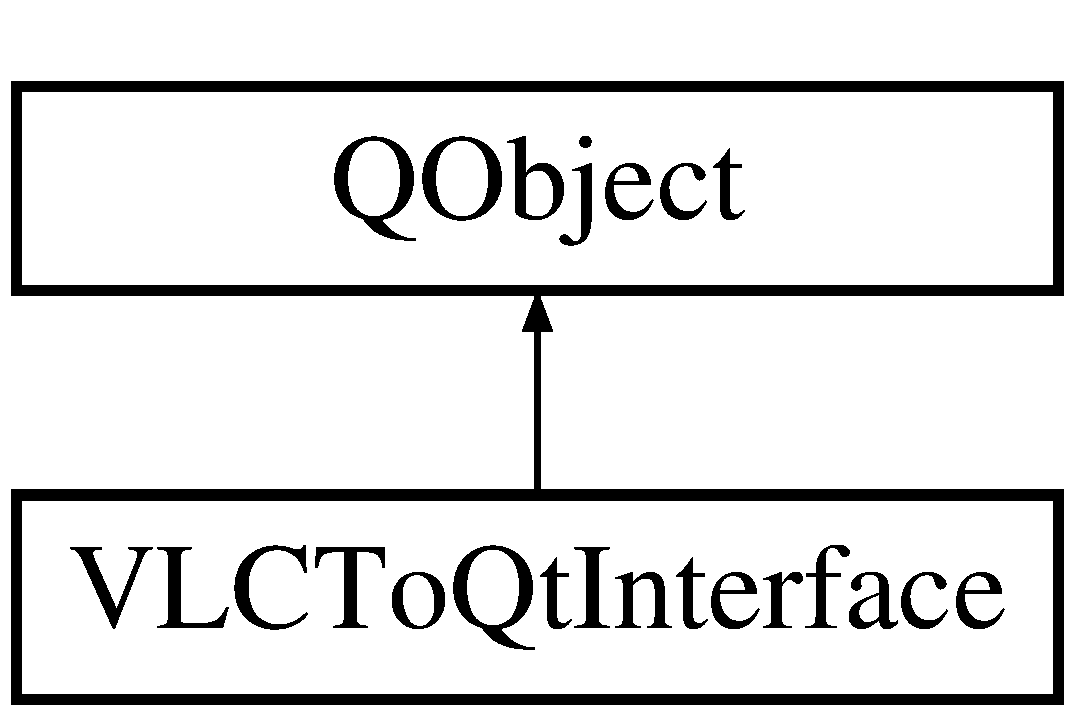
\includegraphics[height=2.000000cm]{classVLCToQtInterface}
\end{center}
\end{figure}
\subsection*{Public Slots}
\begin{DoxyCompactItemize}
\item 
void \hyperlink{classVLCToQtInterface_a93079dc8c7e065a6b9ff2a956e663259}{update\-Video\-Size} ()
\begin{DoxyCompactList}\small\item\em Update video size slot. \end{DoxyCompactList}\end{DoxyCompactItemize}
\subsection*{Signals}
\begin{DoxyCompactItemize}
\item 
void \hyperlink{classVLCToQtInterface_aaf0ae5e8675efd6c039df97c4c24bd77}{resize\-Frame} (int width, int height)
\begin{DoxyCompactList}\small\item\em Signal to resize. \end{DoxyCompactList}\end{DoxyCompactItemize}
\subsection*{Public Member Functions}
\begin{DoxyCompactItemize}
\item 
\hyperlink{classVLCToQtInterface_a782cd983a96f40d16c1f4ba12872e7a1}{V\-L\-C\-To\-Qt\-Interface} ()
\begin{DoxyCompactList}\small\item\em \hyperlink{classVLCToQtInterface}{V\-L\-C\-To\-Qt\-Interface} default value constructor. \end{DoxyCompactList}\item 
\hyperlink{classVLCToQtInterface_ac475e173dea8665cab256a9d8ac59fb2}{V\-L\-C\-To\-Qt\-Interface} (int width, int height)
\begin{DoxyCompactList}\small\item\em \hyperlink{classVLCToQtInterface}{V\-L\-C\-To\-Qt\-Interface} explicit value constructor. \end{DoxyCompactList}\item 
void \hyperlink{classVLCToQtInterface_aaf25e1804b120924ad8b49e36e2bfa8c}{initialize} ()
\begin{DoxyCompactList}\small\item\em Qt interface function to initialize the V\-L\-C client. \end{DoxyCompactList}\item 
virtual \hyperlink{classVLCToQtInterface_aa89b1e15f7e45b93b7ff24aa0a8cbd33}{$\sim$\-V\-L\-C\-To\-Qt\-Interface} ()
\begin{DoxyCompactList}\small\item\em $\sim$\-V\-L\-C\-To\-Qt\-Interface \end{DoxyCompactList}\item 
void \hyperlink{classVLCToQtInterface_af0941bf47aa0a581545f7a367e24185f}{free\-Resources} ()
\begin{DoxyCompactList}\small\item\em Qt interface function to release V\-L\-C allocated resources. \end{DoxyCompactList}\item 
void \hyperlink{classVLCToQtInterface_aea363afecbe6e3b47211eb94d9b918c6}{set\-Media\-To\-File} (const char $\ast$file\-\_\-name)
\begin{DoxyCompactList}\small\item\em Interface to set media to a file. \end{DoxyCompactList}\item 
void \hyperlink{classVLCToQtInterface_a782ba1a8e8d174bd0fabc4d292b6e40e}{set\-Media\-To\-Url} (const char $\ast$url)
\begin{DoxyCompactList}\small\item\em Interface to set the media to a U\-R\-L. \end{DoxyCompactList}\item 
int \hyperlink{classVLCToQtInterface_ac6b8b81ce5f399604b29492654d9f4ca}{play} (uint32\-\_\-t win\-Id)
\begin{DoxyCompactList}\small\item\em Play the media. \end{DoxyCompactList}\item 
int \hyperlink{classVLCToQtInterface_a31f1552dd75dafa174a7b6c4f5d7859f}{play} (void $\ast$win\-Id)
\begin{DoxyCompactList}\small\item\em Play the media. \end{DoxyCompactList}\item 
void \hyperlink{classVLCToQtInterface_a59428645eef3ef14c957a35f5f71a14e}{stop} ()
\begin{DoxyCompactList}\small\item\em Inform the V\-L\-C client to stop playing. \end{DoxyCompactList}\item 
void \hyperlink{classVLCToQtInterface_a69c5cf8921c45d50d0e679447af3c12e}{pause} ()
\begin{DoxyCompactList}\small\item\em Inform the V\-L\-C client to pause. \end{DoxyCompactList}\item 
void \hyperlink{classVLCToQtInterface_a1193d87a92a558d51efc62e6f5639f0a}{set\-Fps} (int fps)
\begin{DoxyCompactList}\small\item\em Sets the frame rate. \end{DoxyCompactList}\item 
void \hyperlink{classVLCToQtInterface_a7928cd122995dd11f7128a768de6015c}{set\-Playback\-Rate} (int fps)
\begin{DoxyCompactList}\small\item\em Set the video playback rate. \end{DoxyCompactList}\item 
bool \hyperlink{classVLCToQtInterface_a10bc62d5d355788f700c7f45ba0713e8}{is\-Playing} ()
\begin{DoxyCompactList}\small\item\em Whether or not the V\-L\-C client is playing. \end{DoxyCompactList}\item 
int \hyperlink{classVLCToQtInterface_a197424c4ed7a829ee6d7d8afa9b377ef}{get\-Fps} ()
\begin{DoxyCompactList}\small\item\em Retrieve the video's frame rate. \end{DoxyCompactList}\item 
bool \hyperlink{classVLCToQtInterface_a8d1084101000873c20c8ebd2b2bdfa13}{get\-Media\-Stats} (\hyperlink{classMediaStatistics}{Media\-Statistics} \&statistics)
\begin{DoxyCompactList}\small\item\em Retrieve the media statistics. \end{DoxyCompactList}\item 
float \hyperlink{classVLCToQtInterface_a7536c3fb0c8cba454414426e2a81239d}{get\-Current\-Bitrate\-Avg} ()
\begin{DoxyCompactList}\small\item\em Interface function to get the average bitrate for the current segment of video. \end{DoxyCompactList}\item 
void \hyperlink{classVLCToQtInterface_ae97936d40e2bd1aaa9bee707353bb8a2}{reset\-Running\-Average} ()
\begin{DoxyCompactList}\small\item\em Reset the running bitrate average. \end{DoxyCompactList}\end{DoxyCompactItemize}


\subsection{Constructor \& Destructor Documentation}
\hypertarget{classVLCToQtInterface_a782cd983a96f40d16c1f4ba12872e7a1}{\index{V\-L\-C\-To\-Qt\-Interface@{V\-L\-C\-To\-Qt\-Interface}!V\-L\-C\-To\-Qt\-Interface@{V\-L\-C\-To\-Qt\-Interface}}
\index{V\-L\-C\-To\-Qt\-Interface@{V\-L\-C\-To\-Qt\-Interface}!VLCToQtInterface@{V\-L\-C\-To\-Qt\-Interface}}
\subsubsection[{V\-L\-C\-To\-Qt\-Interface}]{\setlength{\rightskip}{0pt plus 5cm}V\-L\-C\-To\-Qt\-Interface\-::\-V\-L\-C\-To\-Qt\-Interface (
\begin{DoxyParamCaption}
{}
\end{DoxyParamCaption}
)}}\label{classVLCToQtInterface_a782cd983a96f40d16c1f4ba12872e7a1}


\hyperlink{classVLCToQtInterface}{V\-L\-C\-To\-Qt\-Interface} default value constructor. 


\begin{DoxyCode}
4                                    :
5     m\_width(320),
6     m\_height(240)
7 \{
8     this->initTimer();
9 \}
\end{DoxyCode}
\hypertarget{classVLCToQtInterface_ac475e173dea8665cab256a9d8ac59fb2}{\index{V\-L\-C\-To\-Qt\-Interface@{V\-L\-C\-To\-Qt\-Interface}!V\-L\-C\-To\-Qt\-Interface@{V\-L\-C\-To\-Qt\-Interface}}
\index{V\-L\-C\-To\-Qt\-Interface@{V\-L\-C\-To\-Qt\-Interface}!VLCToQtInterface@{V\-L\-C\-To\-Qt\-Interface}}
\subsubsection[{V\-L\-C\-To\-Qt\-Interface}]{\setlength{\rightskip}{0pt plus 5cm}V\-L\-C\-To\-Qt\-Interface\-::\-V\-L\-C\-To\-Qt\-Interface (
\begin{DoxyParamCaption}
\item[{int}]{width, }
\item[{int}]{height}
\end{DoxyParamCaption}
)}}\label{classVLCToQtInterface_ac475e173dea8665cab256a9d8ac59fb2}


\hyperlink{classVLCToQtInterface}{V\-L\-C\-To\-Qt\-Interface} explicit value constructor. 


\begin{DoxyParams}{Parameters}
{\em width} & The initial video width. \\
\hline
{\em height} & The initial video height. \\
\hline
\end{DoxyParams}

\begin{DoxyCode}
11                                                         :
12     m\_width(width),
13     m\_height(height)
14 \{
15     this->initTimer();
16 \}
\end{DoxyCode}
\hypertarget{classVLCToQtInterface_aa89b1e15f7e45b93b7ff24aa0a8cbd33}{\index{V\-L\-C\-To\-Qt\-Interface@{V\-L\-C\-To\-Qt\-Interface}!$\sim$\-V\-L\-C\-To\-Qt\-Interface@{$\sim$\-V\-L\-C\-To\-Qt\-Interface}}
\index{$\sim$\-V\-L\-C\-To\-Qt\-Interface@{$\sim$\-V\-L\-C\-To\-Qt\-Interface}!VLCToQtInterface@{V\-L\-C\-To\-Qt\-Interface}}
\subsubsection[{$\sim$\-V\-L\-C\-To\-Qt\-Interface}]{\setlength{\rightskip}{0pt plus 5cm}V\-L\-C\-To\-Qt\-Interface\-::$\sim$\-V\-L\-C\-To\-Qt\-Interface (
\begin{DoxyParamCaption}
{}
\end{DoxyParamCaption}
)\hspace{0.3cm}{\ttfamily [virtual]}}}\label{classVLCToQtInterface_aa89b1e15f7e45b93b7ff24aa0a8cbd33}


$\sim$\-V\-L\-C\-To\-Qt\-Interface 


\begin{DoxyCode}
35 \{
36     m\_timer->stop();
37     \textcolor{keyword}{delete} m\_timer;
38 \}
\end{DoxyCode}


\subsection{Member Function Documentation}
\hypertarget{classVLCToQtInterface_af0941bf47aa0a581545f7a367e24185f}{\index{V\-L\-C\-To\-Qt\-Interface@{V\-L\-C\-To\-Qt\-Interface}!free\-Resources@{free\-Resources}}
\index{free\-Resources@{free\-Resources}!VLCToQtInterface@{V\-L\-C\-To\-Qt\-Interface}}
\subsubsection[{free\-Resources}]{\setlength{\rightskip}{0pt plus 5cm}void V\-L\-C\-To\-Qt\-Interface\-::free\-Resources (
\begin{DoxyParamCaption}
{}
\end{DoxyParamCaption}
)}}\label{classVLCToQtInterface_af0941bf47aa0a581545f7a367e24185f}


Qt interface function to release V\-L\-C allocated resources. 


\begin{DoxyCode}
42 \{
43     m\_vlc.\hyperlink{classVLCWrapper_a58462a6c083affe4ac09e057d2303565}{freeResources}();
44 \}
\end{DoxyCode}
\hypertarget{classVLCToQtInterface_a7536c3fb0c8cba454414426e2a81239d}{\index{V\-L\-C\-To\-Qt\-Interface@{V\-L\-C\-To\-Qt\-Interface}!get\-Current\-Bitrate\-Avg@{get\-Current\-Bitrate\-Avg}}
\index{get\-Current\-Bitrate\-Avg@{get\-Current\-Bitrate\-Avg}!VLCToQtInterface@{V\-L\-C\-To\-Qt\-Interface}}
\subsubsection[{get\-Current\-Bitrate\-Avg}]{\setlength{\rightskip}{0pt plus 5cm}float V\-L\-C\-To\-Qt\-Interface\-::get\-Current\-Bitrate\-Avg (
\begin{DoxyParamCaption}
{}
\end{DoxyParamCaption}
)}}\label{classVLCToQtInterface_a7536c3fb0c8cba454414426e2a81239d}


Interface function to get the average bitrate for the current segment of video. 

\begin{DoxyReturn}{Returns}
The average bitrate. 
\end{DoxyReturn}

\begin{DoxyCode}
135 \{
136     \textcolor{keywordflow}{return} m\_vlc.\hyperlink{classVLCWrapper_aff24a01fa335af7febc084c446620070}{getCurrentBitrateAvg}();
137 \}
\end{DoxyCode}
\hypertarget{classVLCToQtInterface_a197424c4ed7a829ee6d7d8afa9b377ef}{\index{V\-L\-C\-To\-Qt\-Interface@{V\-L\-C\-To\-Qt\-Interface}!get\-Fps@{get\-Fps}}
\index{get\-Fps@{get\-Fps}!VLCToQtInterface@{V\-L\-C\-To\-Qt\-Interface}}
\subsubsection[{get\-Fps}]{\setlength{\rightskip}{0pt plus 5cm}int V\-L\-C\-To\-Qt\-Interface\-::get\-Fps (
\begin{DoxyParamCaption}
{}
\end{DoxyParamCaption}
)}}\label{classVLCToQtInterface_a197424c4ed7a829ee6d7d8afa9b377ef}


Retrieve the video's frame rate. 

\begin{DoxyReturn}{Returns}
The frame rate of the video. 
\end{DoxyReturn}

\begin{DoxyCode}
104 \{
105     \textcolor{keywordflow}{return} this->m\_vlc.\hyperlink{classVLCWrapper_a696fd0d152c68c757f9135669cbcbe56}{getFps}();
106 \}
\end{DoxyCode}
\hypertarget{classVLCToQtInterface_a8d1084101000873c20c8ebd2b2bdfa13}{\index{V\-L\-C\-To\-Qt\-Interface@{V\-L\-C\-To\-Qt\-Interface}!get\-Media\-Stats@{get\-Media\-Stats}}
\index{get\-Media\-Stats@{get\-Media\-Stats}!VLCToQtInterface@{V\-L\-C\-To\-Qt\-Interface}}
\subsubsection[{get\-Media\-Stats}]{\setlength{\rightskip}{0pt plus 5cm}bool V\-L\-C\-To\-Qt\-Interface\-::get\-Media\-Stats (
\begin{DoxyParamCaption}
\item[{{\bf Media\-Statistics} \&}]{statistics}
\end{DoxyParamCaption}
)}}\label{classVLCToQtInterface_a8d1084101000873c20c8ebd2b2bdfa13}


Retrieve the media statistics. 

Function to retrieve the statistics of the current media that is playing (i.\-e video bitrate). 
\begin{DoxyParams}{Parameters}
{\em statistics} & \hyperlink{classMediaStatistics}{Media\-Statistics} object to store the statistics in. \\
\hline
\end{DoxyParams}
\begin{DoxyReturn}{Returns}
true if the statistics are retrievable and the video is playing, false otherwise. 
\end{DoxyReturn}

\begin{DoxyCode}
110 \{
111     \textcolor{comment}{//Get the important media statistics to be used by the caller.}
112     \textcolor{keywordtype}{bool} err = \textcolor{keyword}{true};
113     libvlc\_media\_stats\_t stats;
114     \textcolor{keywordflow}{if}((err = m\_vlc.\hyperlink{classVLCWrapper_a743fecb30b118eb999780cc4559eba86}{getMediaStats}(&stats)))
115     \{
116         \textcolor{comment}{//Place in a MediaStatistics object}
117         statistics.\hyperlink{classMediaStatistics_a267abf187ab5690f931d0d7d45407dcc}{setDecodedVideo}(stats.i\_decoded\_video);
118         statistics.\hyperlink{classMediaStatistics_a36bd398cacfada1aaf865374f4bc5e2a}{setDemuxBitrate}(stats.f\_demux\_bitrate);
119         statistics.\hyperlink{classMediaStatistics_a6d9b5760c321c9e189c780ad64cda8f8}{setDemuxCorrupted}(stats.i\_demux\_corrupted);
120         statistics.\hyperlink{classMediaStatistics_a05b13c332cd4ed139392e528b52ac89c}{setDemuxDiscontinuity}(stats.i\_demux\_discontinuity);
121         statistics.\hyperlink{classMediaStatistics_afecbd2e8ebc147b344a9dc18dc6af431}{setDemuxReadBytes}(stats.i\_demux\_read\_bytes);
122         statistics.\hyperlink{classMediaStatistics_ad37d42721c420cea8862cbfd27380a69}{setDisplayedPictures}(stats.i\_displayed\_pictures);
123         statistics.\hyperlink{classMediaStatistics_ad504b337caf39ac04909a4c480101c19}{setInputBitrate}(stats.f\_input\_bitrate);
124         statistics.\hyperlink{classMediaStatistics_a0b305cf428cdc7905d2beb98f08e7c62}{setLostPictures}(stats.i\_lost\_pictures);
125         statistics.\hyperlink{classMediaStatistics_adf378b9efe24da6724583ff13ad98356}{setPlayedPictures}(stats.i\_played\_abuffers);
126         statistics.\hyperlink{classMediaStatistics_a729d2733cd49ad96ab595bb5eb38fe87}{setReadBytes}(stats.i\_read\_bytes);
127 
128     \}
129 
130     \textcolor{keywordflow}{return} err;
131 \}
\end{DoxyCode}
\hypertarget{classVLCToQtInterface_aaf25e1804b120924ad8b49e36e2bfa8c}{\index{V\-L\-C\-To\-Qt\-Interface@{V\-L\-C\-To\-Qt\-Interface}!initialize@{initialize}}
\index{initialize@{initialize}!VLCToQtInterface@{V\-L\-C\-To\-Qt\-Interface}}
\subsubsection[{initialize}]{\setlength{\rightskip}{0pt plus 5cm}void V\-L\-C\-To\-Qt\-Interface\-::initialize (
\begin{DoxyParamCaption}
{}
\end{DoxyParamCaption}
)}}\label{classVLCToQtInterface_aaf25e1804b120924ad8b49e36e2bfa8c}


Qt interface function to initialize the V\-L\-C client. 


\begin{DoxyCode}
30 \{
31     m\_vlc.\hyperlink{classVLCWrapper_a23af9a9003d74b012967e72947141241}{initialize}();
32 \}
\end{DoxyCode}
\hypertarget{classVLCToQtInterface_a10bc62d5d355788f700c7f45ba0713e8}{\index{V\-L\-C\-To\-Qt\-Interface@{V\-L\-C\-To\-Qt\-Interface}!is\-Playing@{is\-Playing}}
\index{is\-Playing@{is\-Playing}!VLCToQtInterface@{V\-L\-C\-To\-Qt\-Interface}}
\subsubsection[{is\-Playing}]{\setlength{\rightskip}{0pt plus 5cm}bool V\-L\-C\-To\-Qt\-Interface\-::is\-Playing (
\begin{DoxyParamCaption}
{}
\end{DoxyParamCaption}
)}}\label{classVLCToQtInterface_a10bc62d5d355788f700c7f45ba0713e8}


Whether or not the V\-L\-C client is playing. 

\begin{DoxyReturn}{Returns}
true if playing, false otherwise 
\end{DoxyReturn}

\begin{DoxyCode}
99 \{
100     \textcolor{keywordflow}{return} m\_vlc.\hyperlink{classVLCWrapper_a52d4cde1548105d10d1b8906fac68dac}{isPlaying}();
101 \}
\end{DoxyCode}
\hypertarget{classVLCToQtInterface_a69c5cf8921c45d50d0e679447af3c12e}{\index{V\-L\-C\-To\-Qt\-Interface@{V\-L\-C\-To\-Qt\-Interface}!pause@{pause}}
\index{pause@{pause}!VLCToQtInterface@{V\-L\-C\-To\-Qt\-Interface}}
\subsubsection[{pause}]{\setlength{\rightskip}{0pt plus 5cm}void V\-L\-C\-To\-Qt\-Interface\-::pause (
\begin{DoxyParamCaption}
{}
\end{DoxyParamCaption}
)}}\label{classVLCToQtInterface_a69c5cf8921c45d50d0e679447af3c12e}


Inform the V\-L\-C client to pause. 


\begin{DoxyCode}
83 \{
84     m\_vlc.\hyperlink{classVLCWrapper_a8dadd74aef3a683cf73b677bc98db70c}{pause}();
85 \}
\end{DoxyCode}
\hypertarget{classVLCToQtInterface_ac6b8b81ce5f399604b29492654d9f4ca}{\index{V\-L\-C\-To\-Qt\-Interface@{V\-L\-C\-To\-Qt\-Interface}!play@{play}}
\index{play@{play}!VLCToQtInterface@{V\-L\-C\-To\-Qt\-Interface}}
\subsubsection[{play}]{\setlength{\rightskip}{0pt plus 5cm}int V\-L\-C\-To\-Qt\-Interface\-::play (
\begin{DoxyParamCaption}
\item[{uint32\-\_\-t}]{win\-Id}
\end{DoxyParamCaption}
)}}\label{classVLCToQtInterface_ac6b8b81ce5f399604b29492654d9f4ca}


Play the media. 

This interface function will inform the V\-L\-C client to begin playing, displaying the video in using the passed window handle. 
\begin{DoxyParams}{Parameters}
{\em win\-Id} & The handle to an X\-Window window (Linux). \\
\hline
\end{DoxyParams}
\begin{DoxyReturn}{Returns}
0 on success, -\/1 on failure. 
\end{DoxyReturn}

\begin{DoxyCode}
62 \{
63     \textcolor{keywordtype}{int} status = 0;
64 
65     status = m\_vlc.\hyperlink{classVLCWrapper_a75bc08d5b5d25ebcbdd50d3ecd1301bd}{play}(winId);
66 
67     \textcolor{keywordflow}{return} status;
68 \}
\end{DoxyCode}
\hypertarget{classVLCToQtInterface_a31f1552dd75dafa174a7b6c4f5d7859f}{\index{V\-L\-C\-To\-Qt\-Interface@{V\-L\-C\-To\-Qt\-Interface}!play@{play}}
\index{play@{play}!VLCToQtInterface@{V\-L\-C\-To\-Qt\-Interface}}
\subsubsection[{play}]{\setlength{\rightskip}{0pt plus 5cm}int V\-L\-C\-To\-Qt\-Interface\-::play (
\begin{DoxyParamCaption}
\item[{void $\ast$}]{win\-Id}
\end{DoxyParamCaption}
)}}\label{classVLCToQtInterface_a31f1552dd75dafa174a7b6c4f5d7859f}


Play the media. 

This interface function will inform the V\-L\-C client to begin playing, displaying the video in using the passed window handle. 
\begin{DoxyParams}{Parameters}
{\em win\-Id} & The handle to an H\-W\-N\-D window (Windows). \\
\hline
\end{DoxyParams}
\begin{DoxyReturn}{Returns}
0 on success, -\/1 on failure. 
\end{DoxyReturn}

\begin{DoxyCode}
71 \{
72     \textcolor{keywordtype}{int} status = 0;
73     status = m\_vlc.\hyperlink{classVLCWrapper_a75bc08d5b5d25ebcbdd50d3ecd1301bd}{play}(winId);
74     \textcolor{keywordflow}{return} status;
75 \}
\end{DoxyCode}
\hypertarget{classVLCToQtInterface_ae97936d40e2bd1aaa9bee707353bb8a2}{\index{V\-L\-C\-To\-Qt\-Interface@{V\-L\-C\-To\-Qt\-Interface}!reset\-Running\-Average@{reset\-Running\-Average}}
\index{reset\-Running\-Average@{reset\-Running\-Average}!VLCToQtInterface@{V\-L\-C\-To\-Qt\-Interface}}
\subsubsection[{reset\-Running\-Average}]{\setlength{\rightskip}{0pt plus 5cm}void V\-L\-C\-To\-Qt\-Interface\-::reset\-Running\-Average (
\begin{DoxyParamCaption}
{}
\end{DoxyParamCaption}
)}}\label{classVLCToQtInterface_ae97936d40e2bd1aaa9bee707353bb8a2}


Reset the running bitrate average. 

Interface function to reset the running average of the video bitrate (as in when a new segment of video is started). 
\begin{DoxyCode}
141 \{
142     m\_vlc.\hyperlink{classVLCWrapper_a5acd0eb82102874f09dacaa277a2f784}{resetRunningAverage}();
143 \}
\end{DoxyCode}
\hypertarget{classVLCToQtInterface_aaf0ae5e8675efd6c039df97c4c24bd77}{\index{V\-L\-C\-To\-Qt\-Interface@{V\-L\-C\-To\-Qt\-Interface}!resize\-Frame@{resize\-Frame}}
\index{resize\-Frame@{resize\-Frame}!VLCToQtInterface@{V\-L\-C\-To\-Qt\-Interface}}
\subsubsection[{resize\-Frame}]{\setlength{\rightskip}{0pt plus 5cm}void V\-L\-C\-To\-Qt\-Interface\-::resize\-Frame (
\begin{DoxyParamCaption}
\item[{int}]{width, }
\item[{int}]{height}
\end{DoxyParamCaption}
)\hspace{0.3cm}{\ttfamily [signal]}}}\label{classVLCToQtInterface_aaf0ae5e8675efd6c039df97c4c24bd77}


Signal to resize. 

Signal that is emitted to inform the containing widget to resize the video frame. 
\begin{DoxyParams}{Parameters}
{\em width} & The new frame width. \\
\hline
{\em height} & The new frame height. \\
\hline
\end{DoxyParams}
\hypertarget{classVLCToQtInterface_a1193d87a92a558d51efc62e6f5639f0a}{\index{V\-L\-C\-To\-Qt\-Interface@{V\-L\-C\-To\-Qt\-Interface}!set\-Fps@{set\-Fps}}
\index{set\-Fps@{set\-Fps}!VLCToQtInterface@{V\-L\-C\-To\-Qt\-Interface}}
\subsubsection[{set\-Fps}]{\setlength{\rightskip}{0pt plus 5cm}void V\-L\-C\-To\-Qt\-Interface\-::set\-Fps (
\begin{DoxyParamCaption}
\item[{int}]{fps}
\end{DoxyParamCaption}
)}}\label{classVLCToQtInterface_a1193d87a92a558d51efc62e6f5639f0a}


Sets the frame rate. 

Set the frame rate of the video to be played. 
\begin{DoxyParams}{Parameters}
{\em fps} & The frame rate. \\
\hline
\end{DoxyParams}

\begin{DoxyCode}
88 \{
89     this->m\_vlc.\hyperlink{classVLCWrapper_abb027f9dfb30636141f85a1292885634}{setFps}(fps);
90 \}
\end{DoxyCode}
\hypertarget{classVLCToQtInterface_aea363afecbe6e3b47211eb94d9b918c6}{\index{V\-L\-C\-To\-Qt\-Interface@{V\-L\-C\-To\-Qt\-Interface}!set\-Media\-To\-File@{set\-Media\-To\-File}}
\index{set\-Media\-To\-File@{set\-Media\-To\-File}!VLCToQtInterface@{V\-L\-C\-To\-Qt\-Interface}}
\subsubsection[{set\-Media\-To\-File}]{\setlength{\rightskip}{0pt plus 5cm}void V\-L\-C\-To\-Qt\-Interface\-::set\-Media\-To\-File (
\begin{DoxyParamCaption}
\item[{const char $\ast$}]{file\-\_\-name}
\end{DoxyParamCaption}
)}}\label{classVLCToQtInterface_aea363afecbe6e3b47211eb94d9b918c6}


Interface to set media to a file. 

Sets the V\-L\-C client's media object to play a certain file. 
\begin{DoxyParams}{Parameters}
{\em file\-\_\-name} & The path to the file to play. \\
\hline
\end{DoxyParams}

\begin{DoxyCode}
48 \{
49     \textcolor{comment}{//Open the file specified in the open string}
50     m\_vlc.\hyperlink{classVLCWrapper_a9f5993525559efb2fbdd434c79f040c7}{setMediaToFile}(file\_name);
51 \}
\end{DoxyCode}
\hypertarget{classVLCToQtInterface_a782ba1a8e8d174bd0fabc4d292b6e40e}{\index{V\-L\-C\-To\-Qt\-Interface@{V\-L\-C\-To\-Qt\-Interface}!set\-Media\-To\-Url@{set\-Media\-To\-Url}}
\index{set\-Media\-To\-Url@{set\-Media\-To\-Url}!VLCToQtInterface@{V\-L\-C\-To\-Qt\-Interface}}
\subsubsection[{set\-Media\-To\-Url}]{\setlength{\rightskip}{0pt plus 5cm}void V\-L\-C\-To\-Qt\-Interface\-::set\-Media\-To\-Url (
\begin{DoxyParamCaption}
\item[{const char $\ast$}]{url}
\end{DoxyParamCaption}
)}}\label{classVLCToQtInterface_a782ba1a8e8d174bd0fabc4d292b6e40e}


Interface to set the media to a U\-R\-L. 

Sets the V\-L\-C client's media object to stream from a specified U\-R\-L. 
\begin{DoxyParams}{Parameters}
{\em url} & The U\-R\-L of the media to stream. \\
\hline
\end{DoxyParams}

\begin{DoxyCode}
55 \{
56     \textcolor{comment}{//Open specified url}
57     m\_vlc.\hyperlink{classVLCWrapper_a9f5993525559efb2fbdd434c79f040c7}{setMediaToFile}(url);
58 \}
\end{DoxyCode}
\hypertarget{classVLCToQtInterface_a7928cd122995dd11f7128a768de6015c}{\index{V\-L\-C\-To\-Qt\-Interface@{V\-L\-C\-To\-Qt\-Interface}!set\-Playback\-Rate@{set\-Playback\-Rate}}
\index{set\-Playback\-Rate@{set\-Playback\-Rate}!VLCToQtInterface@{V\-L\-C\-To\-Qt\-Interface}}
\subsubsection[{set\-Playback\-Rate}]{\setlength{\rightskip}{0pt plus 5cm}void V\-L\-C\-To\-Qt\-Interface\-::set\-Playback\-Rate (
\begin{DoxyParamCaption}
\item[{int}]{fps}
\end{DoxyParamCaption}
)}}\label{classVLCToQtInterface_a7928cd122995dd11f7128a768de6015c}


Set the video playback rate. 

Set the V\-L\-C client's video playback rate. 
\begin{DoxyParams}{Parameters}
{\em fps} & The playback rate. \\
\hline
\end{DoxyParams}

\begin{DoxyCode}
93 \{
94     this->m\_vlc.\hyperlink{classVLCWrapper_a7d2f4f7b0f796711b614f2d9f6ea63ee}{resetMedia}(fps);
95 \}
\end{DoxyCode}
\hypertarget{classVLCToQtInterface_a59428645eef3ef14c957a35f5f71a14e}{\index{V\-L\-C\-To\-Qt\-Interface@{V\-L\-C\-To\-Qt\-Interface}!stop@{stop}}
\index{stop@{stop}!VLCToQtInterface@{V\-L\-C\-To\-Qt\-Interface}}
\subsubsection[{stop}]{\setlength{\rightskip}{0pt plus 5cm}void V\-L\-C\-To\-Qt\-Interface\-::stop (
\begin{DoxyParamCaption}
{}
\end{DoxyParamCaption}
)}}\label{classVLCToQtInterface_a59428645eef3ef14c957a35f5f71a14e}


Inform the V\-L\-C client to stop playing. 


\begin{DoxyCode}
78 \{
79     m\_vlc.\hyperlink{classVLCWrapper_a2ddae6b4fb05cd9cd149c6769d8fa7a9}{stop}();
80 \}
\end{DoxyCode}
\hypertarget{classVLCToQtInterface_a93079dc8c7e065a6b9ff2a956e663259}{\index{V\-L\-C\-To\-Qt\-Interface@{V\-L\-C\-To\-Qt\-Interface}!update\-Video\-Size@{update\-Video\-Size}}
\index{update\-Video\-Size@{update\-Video\-Size}!VLCToQtInterface@{V\-L\-C\-To\-Qt\-Interface}}
\subsubsection[{update\-Video\-Size}]{\setlength{\rightskip}{0pt plus 5cm}void V\-L\-C\-To\-Qt\-Interface\-::update\-Video\-Size (
\begin{DoxyParamCaption}
{}
\end{DoxyParamCaption}
)\hspace{0.3cm}{\ttfamily [slot]}}}\label{classVLCToQtInterface_a93079dc8c7e065a6b9ff2a956e663259}


Update video size slot. 

Slot that is called from a timer to determine if the parent widget needs to resize the video container. 
\begin{DoxyCode}
148 \{
149     \textcolor{keywordtype}{int} width = 0, height = 0;
150     \textcolor{comment}{//Get width and height, store in local variabled, return if video is playing}
151     \textcolor{keywordtype}{bool} playing = m\_vlc.\hyperlink{classVLCWrapper_a806ad002020aaba2f471ee948226cb0c}{getVideoSize}(&width, &height);
152     \textcolor{comment}{//If video is playing}
153     \textcolor{keywordflow}{if}(playing)
154     \{
155         \textcolor{keywordflow}{if}(width == 0 && height == 0)
156         \{
157             \textcolor{comment}{//Set new widths and heights and emit resize signal}
158             \textcolor{comment}{//this->m\_width = 320;}
159             \textcolor{comment}{//this->m\_height = 240;}
160             emit \hyperlink{classVLCToQtInterface_aaf0ae5e8675efd6c039df97c4c24bd77}{resizeFrame}(m\_width, m\_height);
161         \}
162         \textcolor{comment}{//If width and height are different}
163         \textcolor{keywordflow}{else} \textcolor{keywordflow}{if}((width) != this->m\_width || (height) != this->m\_height)
164         \{
165             \textcolor{comment}{//Set new widths and heights and emit resize signal}
166             this->m\_width = width;
167             this->m\_height = height;
168             emit \hyperlink{classVLCToQtInterface_aaf0ae5e8675efd6c039df97c4c24bd77}{resizeFrame}(width, height);
169         \}
170 
171     \}
172     \textcolor{keywordflow}{else}
173     \{
174         \textcolor{keywordflow}{if}((width) != 320 && (height) != 240)
175         \{
176             this->m\_width = 320;
177             this->m\_height = 240;
178             emit \hyperlink{classVLCToQtInterface_aaf0ae5e8675efd6c039df97c4c24bd77}{resizeFrame}(m\_width, m\_height);
179         \}
180 
181     \}
182 
183     \textcolor{comment}{//Get media stats}
184     \textcolor{keywordflow}{if}(m\_vlc.\hyperlink{classVLCWrapper_a52d4cde1548105d10d1b8906fac68dac}{isPlaying}())
185         this->m\_vlc.\hyperlink{classVLCWrapper_a743fecb30b118eb999780cc4559eba86}{getMediaStats}();
186 \}
\end{DoxyCode}


The documentation for this class was generated from the following files\-:\begin{DoxyCompactItemize}
\item 
Video/\hyperlink{vlctoqtinterface_8h}{vlctoqtinterface.\-h}\item 
Video/\hyperlink{vlctoqtinterface_8cpp}{vlctoqtinterface.\-cpp}\end{DoxyCompactItemize}

\hypertarget{classVLCVideoWidget}{\section{V\-L\-C\-Video\-Widget Class Reference}
\label{classVLCVideoWidget}\index{V\-L\-C\-Video\-Widget@{V\-L\-C\-Video\-Widget}}
}


This class defines a widget that uses a V\-L\-C client to display video.  




{\ttfamily \#include $<$vlcvideowidget.\-h$>$}

Inheritance diagram for V\-L\-C\-Video\-Widget\-:\begin{figure}[H]
\begin{center}
\leavevmode
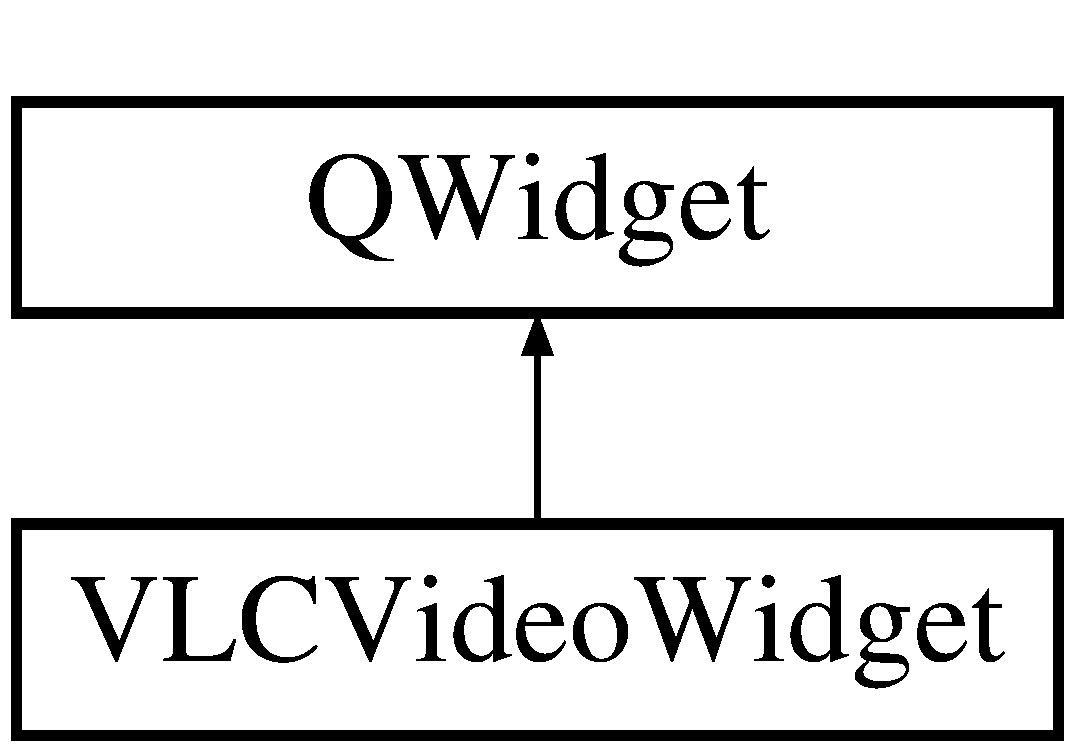
\includegraphics[height=2.000000cm]{classVLCVideoWidget}
\end{center}
\end{figure}
\subsection*{Public Slots}
\begin{DoxyCompactItemize}
\item 
void \hyperlink{classVLCVideoWidget_aff4501569b0e46b3641625c3c9bbd5c6}{video\-Resized} (int width, int height)
\begin{DoxyCompactList}\small\item\em A slot invoked when the size of the video changes. \end{DoxyCompactList}\end{DoxyCompactItemize}
\subsection*{Signals}
\begin{DoxyCompactItemize}
\item 
void \hyperlink{classVLCVideoWidget_aeff3477d9c077d45b0ff8caea2514150}{resize\-Parent} (int width, int height)
\end{DoxyCompactItemize}
\subsection*{Public Member Functions}
\begin{DoxyCompactItemize}
\item 
\hyperlink{classVLCVideoWidget_a2ee422ecbf1d7c6a09c8c08461ae8f0d}{V\-L\-C\-Video\-Widget} (Q\-Widget $\ast$parent=0)
\begin{DoxyCompactList}\small\item\em Explicit value constructor. \end{DoxyCompactList}\item 
\hyperlink{classVLCVideoWidget_a2ad9c4a037fdb833b1b1f9ba71075d86}{$\sim$\-V\-L\-C\-Video\-Widget} ()
\item 
void \hyperlink{classVLCVideoWidget_a7eb5395abd53f19c012fea779b6bac1e}{play\-File} (Q\-String file)
\begin{DoxyCompactList}\small\item\em Play a video from a file on this widget. \end{DoxyCompactList}\item 
void \hyperlink{classVLCVideoWidget_a1119aa3a41789fc1f4abe834e36c64df}{play\-Url} (Q\-String url)
\begin{DoxyCompactList}\small\item\em Stream the video at this U\-R\-L. \end{DoxyCompactList}\item 
void \hyperlink{classVLCVideoWidget_aefa842a30cbb11522428597c1f0608a0}{stop\-Playing} ()
\begin{DoxyCompactList}\small\item\em Stop playing the video. \end{DoxyCompactList}\item 
bool \hyperlink{classVLCVideoWidget_a45fd49c0a63d1eeeaaff78ffd208ddad}{is\-Playing} ()
\begin{DoxyCompactList}\small\item\em Determine if the video is playing. \end{DoxyCompactList}\item 
void \hyperlink{classVLCVideoWidget_a5fce57e1a69fd7371c7e0950d5bb14a8}{set\-Fps} (int fps)
\begin{DoxyCompactList}\small\item\em Set the frame rate of the playing video. \end{DoxyCompactList}\item 
int \hyperlink{classVLCVideoWidget_ac80ca2be7b8f96631f32827ab06e70a1}{get\-Fps} ()
\begin{DoxyCompactList}\small\item\em Get the frame rate of the video. \end{DoxyCompactList}\item 
void \hyperlink{classVLCVideoWidget_aff2bdf48d08757e6b86aa5f21eb43fb5}{set\-Playback\-Rate} (int fps)
\begin{DoxyCompactList}\small\item\em Set the V\-L\-C client playback rate. \end{DoxyCompactList}\item 
void \hyperlink{classVLCVideoWidget_af6bfaebcb882449195ea2a5e5918ee57}{reset\-Stats} ()
\begin{DoxyCompactList}\small\item\em Reset the values of the statistics captured from the V\-L\-C client for the current video. \end{DoxyCompactList}\item 
float \hyperlink{classVLCVideoWidget_a61dcea162c69c8e831dc193ccf8271e6}{get\-Average\-Bitrate} ()
\begin{DoxyCompactList}\small\item\em Get the current running average of the input bitrate. \end{DoxyCompactList}\end{DoxyCompactItemize}
\subsection*{Protected Member Functions}
\begin{DoxyCompactItemize}
\item 
void \hyperlink{classVLCVideoWidget_ae6a2d91395f32ad7c80fb1839557da4f}{key\-Press\-Event} (Q\-Key\-Event $\ast$e)
\item 
void \hyperlink{classVLCVideoWidget_a2fb0969c2a4efa024038ce1e1cfe1e64}{paint\-Event} (Q\-Paint\-Event $\ast$e)
\end{DoxyCompactItemize}


\subsection{Detailed Description}
This class defines a widget that uses a V\-L\-C client to display video. 

\subsection{Constructor \& Destructor Documentation}
\hypertarget{classVLCVideoWidget_a2ee422ecbf1d7c6a09c8c08461ae8f0d}{\index{V\-L\-C\-Video\-Widget@{V\-L\-C\-Video\-Widget}!V\-L\-C\-Video\-Widget@{V\-L\-C\-Video\-Widget}}
\index{V\-L\-C\-Video\-Widget@{V\-L\-C\-Video\-Widget}!VLCVideoWidget@{V\-L\-C\-Video\-Widget}}
\subsubsection[{V\-L\-C\-Video\-Widget}]{\setlength{\rightskip}{0pt plus 5cm}V\-L\-C\-Video\-Widget\-::\-V\-L\-C\-Video\-Widget (
\begin{DoxyParamCaption}
\item[{Q\-Widget $\ast$}]{parent = {\ttfamily 0}}
\end{DoxyParamCaption}
)\hspace{0.3cm}{\ttfamily [explicit]}}}\label{classVLCVideoWidget_a2ee422ecbf1d7c6a09c8c08461ae8f0d}


Explicit value constructor. 


\begin{DoxyParams}{Parameters}
{\em parent} & The parent widget. \\
\hline
\end{DoxyParams}

\begin{DoxyCode}
15                                               :
16     QWidget(parent)
17 \{
18 
19 \textcolor{comment}{//    //Set up sliders and timer}
20 \textcolor{comment}{//    m\_volumeSlider=new QSlider(Qt::Horizontal,this);}
21 \textcolor{comment}{//    m\_volumeSlider->setMaximum(100); //the volume is between 0 and 100}
22 \textcolor{comment}{//    m\_volumeSlider->setToolTip("Audio slider");}
23 
24 \textcolor{comment}{//    // Note: if you use streaming, there is no ability to use the position slider}
25 \textcolor{comment}{//    m\_positionSlider=new QSlider(Qt::Horizontal,this);}
26 \textcolor{comment}{//    m\_positionSlider->setMaximum(POSITION\_RESOLUTION);}
27 
28     m\_poller = \textcolor{keyword}{new} QTimer(\textcolor{keyword}{this});
29 
30     \textcolor{comment}{//Get a qframe for the video widget}
31     m\_videoWidget = \textcolor{keyword}{new} QFrame(\textcolor{keyword}{this});
32 
33     \textcolor{comment}{//Set up the box layout}
34     \textcolor{comment}{//QVBoxLayout *layout = new QVBoxLayout;}
35     \textcolor{comment}{//layout->addWidget(m\_videoWidget);}
36 \textcolor{comment}{//    layout->addWidget(m\_volumeSlider);}
37 \textcolor{comment}{//    layout->addWidget(m\_positionSlider);}
38     \textcolor{comment}{//setLayout(layout);}
39 
40     \textcolor{comment}{//m\_videoWidget->setStyleSheet("background-color:black;");}
41     m\_videoWidget->resize(\hyperlink{vlcvideowidget_8h_a2deec7650a0c6caf3c17a5ddf36d6460}{VIDEOWIDGET\_DEFAULT\_WIDTH}, 
      \hyperlink{vlcvideowidget_8h_afea1bcfd5eabc718d60a92aee2cd7f50}{VIDEOWIDGET\_DEFAULT\_HEIGHT});
42     \textcolor{comment}{//Signals and slots connections}
43 \textcolor{comment}{//    connect(m\_poller, SIGNAL(timeout()), this, SLOT(updateInterface()));}
44 \textcolor{comment}{//    connect(m\_volumeSlider, SIGNAL(sliderMoved(int)), this, SLOT(changeVolume(int)));}
45 \textcolor{comment}{//    connect(m\_positionSlider, SIGNAL(sliderMoved(int)), this, SLOT(changePosition(int)));}
46     m\_vlc\_interface = \textcolor{keyword}{new} \hyperlink{classVLCToQtInterface}{VLCToQtInterface}(m\_videoWidget->width(), m\_videoWidget->height())
      ;
47     m\_vlc\_interface->\hyperlink{classVLCToQtInterface_aaf25e1804b120924ad8b49e36e2bfa8c}{initialize}();
48     m\_poller->start(10);
49 
50     connect(m\_vlc\_interface, SIGNAL(resizeFrame(\textcolor{keywordtype}{int},\textcolor{keywordtype}{int})), \textcolor{keyword}{this}, SLOT(
      \hyperlink{classVLCVideoWidget_aff4501569b0e46b3641625c3c9bbd5c6}{videoResized}(\textcolor{keywordtype}{int},\textcolor{keywordtype}{int})));
51 \}
\end{DoxyCode}
\hypertarget{classVLCVideoWidget_a2ad9c4a037fdb833b1b1f9ba71075d86}{\index{V\-L\-C\-Video\-Widget@{V\-L\-C\-Video\-Widget}!$\sim$\-V\-L\-C\-Video\-Widget@{$\sim$\-V\-L\-C\-Video\-Widget}}
\index{$\sim$\-V\-L\-C\-Video\-Widget@{$\sim$\-V\-L\-C\-Video\-Widget}!VLCVideoWidget@{V\-L\-C\-Video\-Widget}}
\subsubsection[{$\sim$\-V\-L\-C\-Video\-Widget}]{\setlength{\rightskip}{0pt plus 5cm}V\-L\-C\-Video\-Widget\-::$\sim$\-V\-L\-C\-Video\-Widget (
\begin{DoxyParamCaption}
{}
\end{DoxyParamCaption}
)}}\label{classVLCVideoWidget_a2ad9c4a037fdb833b1b1f9ba71075d86}

\begin{DoxyCode}
54 \{
55     this->\hyperlink{classVLCVideoWidget_aefa842a30cbb11522428597c1f0608a0}{stopPlaying}();
56     \textcolor{keyword}{delete} m\_videoWidget;
57     \textcolor{comment}{//delete m\_volumeSlider;}
58     m\_poller->stop();
59     \textcolor{keyword}{delete} m\_poller;
60     \textcolor{comment}{//delete m\_positionSlider;}
61     \textcolor{keyword}{delete} m\_vlc\_interface;
62 
63 
64 \}
\end{DoxyCode}


\subsection{Member Function Documentation}
\hypertarget{classVLCVideoWidget_a61dcea162c69c8e831dc193ccf8271e6}{\index{V\-L\-C\-Video\-Widget@{V\-L\-C\-Video\-Widget}!get\-Average\-Bitrate@{get\-Average\-Bitrate}}
\index{get\-Average\-Bitrate@{get\-Average\-Bitrate}!VLCVideoWidget@{V\-L\-C\-Video\-Widget}}
\subsubsection[{get\-Average\-Bitrate}]{\setlength{\rightskip}{0pt plus 5cm}float V\-L\-C\-Video\-Widget\-::get\-Average\-Bitrate (
\begin{DoxyParamCaption}
{}
\end{DoxyParamCaption}
)}}\label{classVLCVideoWidget_a61dcea162c69c8e831dc193ccf8271e6}


Get the current running average of the input bitrate. 

\begin{DoxyReturn}{Returns}
The averate data rate. 
\end{DoxyReturn}

\begin{DoxyCode}
111 \{
112     \textcolor{keywordflow}{return} this->m\_vlc\_interface->\hyperlink{classVLCToQtInterface_a7536c3fb0c8cba454414426e2a81239d}{getCurrentBitrateAvg}();
113 \}
\end{DoxyCode}
\hypertarget{classVLCVideoWidget_ac80ca2be7b8f96631f32827ab06e70a1}{\index{V\-L\-C\-Video\-Widget@{V\-L\-C\-Video\-Widget}!get\-Fps@{get\-Fps}}
\index{get\-Fps@{get\-Fps}!VLCVideoWidget@{V\-L\-C\-Video\-Widget}}
\subsubsection[{get\-Fps}]{\setlength{\rightskip}{0pt plus 5cm}int V\-L\-C\-Video\-Widget\-::get\-Fps (
\begin{DoxyParamCaption}
{}
\end{DoxyParamCaption}
)}}\label{classVLCVideoWidget_ac80ca2be7b8f96631f32827ab06e70a1}


Get the frame rate of the video. 

\begin{DoxyReturn}{Returns}
The video frame rate. 
\end{DoxyReturn}

\begin{DoxyCode}
96 \{
97     \textcolor{keywordflow}{return} m\_vlc\_interface->\hyperlink{classVLCToQtInterface_a197424c4ed7a829ee6d7d8afa9b377ef}{getFps}();
98 \}
\end{DoxyCode}
\hypertarget{classVLCVideoWidget_a45fd49c0a63d1eeeaaff78ffd208ddad}{\index{V\-L\-C\-Video\-Widget@{V\-L\-C\-Video\-Widget}!is\-Playing@{is\-Playing}}
\index{is\-Playing@{is\-Playing}!VLCVideoWidget@{V\-L\-C\-Video\-Widget}}
\subsubsection[{is\-Playing}]{\setlength{\rightskip}{0pt plus 5cm}bool V\-L\-C\-Video\-Widget\-::is\-Playing (
\begin{DoxyParamCaption}
{}
\end{DoxyParamCaption}
)}}\label{classVLCVideoWidget_a45fd49c0a63d1eeeaaff78ffd208ddad}


Determine if the video is playing. 

\begin{DoxyReturn}{Returns}
True if the video is playing. 
\end{DoxyReturn}

\begin{DoxyCode}
86 \{
87     \textcolor{keywordflow}{return} this->m\_vlc\_interface->\hyperlink{classVLCToQtInterface_a10bc62d5d355788f700c7f45ba0713e8}{isPlaying}();
88 \}
\end{DoxyCode}
\hypertarget{classVLCVideoWidget_ae6a2d91395f32ad7c80fb1839557da4f}{\index{V\-L\-C\-Video\-Widget@{V\-L\-C\-Video\-Widget}!key\-Press\-Event@{key\-Press\-Event}}
\index{key\-Press\-Event@{key\-Press\-Event}!VLCVideoWidget@{V\-L\-C\-Video\-Widget}}
\subsubsection[{key\-Press\-Event}]{\setlength{\rightskip}{0pt plus 5cm}void V\-L\-C\-Video\-Widget\-::key\-Press\-Event (
\begin{DoxyParamCaption}
\item[{Q\-Key\-Event $\ast$}]{e}
\end{DoxyParamCaption}
)\hspace{0.3cm}{\ttfamily [protected]}}}\label{classVLCVideoWidget_ae6a2d91395f32ad7c80fb1839557da4f}

\begin{DoxyCode}
145 \{
146     \textcolor{keywordflow}{if}(e->key() == Qt::Key\_Down)
147     \{
148         this->\hyperlink{classVLCVideoWidget_aefa842a30cbb11522428597c1f0608a0}{stopPlaying}();
149     \}
150 \}
\end{DoxyCode}
\hypertarget{classVLCVideoWidget_a2fb0969c2a4efa024038ce1e1cfe1e64}{\index{V\-L\-C\-Video\-Widget@{V\-L\-C\-Video\-Widget}!paint\-Event@{paint\-Event}}
\index{paint\-Event@{paint\-Event}!VLCVideoWidget@{V\-L\-C\-Video\-Widget}}
\subsubsection[{paint\-Event}]{\setlength{\rightskip}{0pt plus 5cm}void V\-L\-C\-Video\-Widget\-::paint\-Event (
\begin{DoxyParamCaption}
\item[{Q\-Paint\-Event $\ast$}]{e}
\end{DoxyParamCaption}
)\hspace{0.3cm}{\ttfamily [protected]}}}\label{classVLCVideoWidget_a2fb0969c2a4efa024038ce1e1cfe1e64}

\begin{DoxyCode}
125 \{
126     QStyleOption opt;
127     opt.init(\textcolor{keyword}{this});
128     QPainter p(\textcolor{keyword}{this});
129     style()->drawPrimitive(QStyle::PE\_Widget, &opt, &p, \textcolor{keyword}{this});
130 \}
\end{DoxyCode}
\hypertarget{classVLCVideoWidget_a7eb5395abd53f19c012fea779b6bac1e}{\index{V\-L\-C\-Video\-Widget@{V\-L\-C\-Video\-Widget}!play\-File@{play\-File}}
\index{play\-File@{play\-File}!VLCVideoWidget@{V\-L\-C\-Video\-Widget}}
\subsubsection[{play\-File}]{\setlength{\rightskip}{0pt plus 5cm}void V\-L\-C\-Video\-Widget\-::play\-File (
\begin{DoxyParamCaption}
\item[{Q\-String}]{file}
\end{DoxyParamCaption}
)}}\label{classVLCVideoWidget_a7eb5395abd53f19c012fea779b6bac1e}


Play a video from a file on this widget. 


\begin{DoxyParams}{Parameters}
{\em file} & The path of the file to play. \\
\hline
\end{DoxyParams}

\begin{DoxyCode}
67 \{
68     m\_vlc\_interface->\hyperlink{classVLCToQtInterface_aea363afecbe6e3b47211eb94d9b918c6}{setMediaToFile}(file.toStdString().c\_str());
69     this->openMedia();
70 \}
\end{DoxyCode}
\hypertarget{classVLCVideoWidget_a1119aa3a41789fc1f4abe834e36c64df}{\index{V\-L\-C\-Video\-Widget@{V\-L\-C\-Video\-Widget}!play\-Url@{play\-Url}}
\index{play\-Url@{play\-Url}!VLCVideoWidget@{V\-L\-C\-Video\-Widget}}
\subsubsection[{play\-Url}]{\setlength{\rightskip}{0pt plus 5cm}void V\-L\-C\-Video\-Widget\-::play\-Url (
\begin{DoxyParamCaption}
\item[{Q\-String}]{url}
\end{DoxyParamCaption}
)}}\label{classVLCVideoWidget_a1119aa3a41789fc1f4abe834e36c64df}


Stream the video at this U\-R\-L. 


\begin{DoxyParams}{Parameters}
{\em url} & The U\-R\-L to stream video from. \\
\hline
\end{DoxyParams}

\begin{DoxyCode}
73 \{
74     m\_vlc\_interface->\hyperlink{classVLCToQtInterface_a782ba1a8e8d174bd0fabc4d292b6e40e}{setMediaToUrl}(url.toStdString().c\_str());
75     this->openMedia();
76 \}
\end{DoxyCode}
\hypertarget{classVLCVideoWidget_af6bfaebcb882449195ea2a5e5918ee57}{\index{V\-L\-C\-Video\-Widget@{V\-L\-C\-Video\-Widget}!reset\-Stats@{reset\-Stats}}
\index{reset\-Stats@{reset\-Stats}!VLCVideoWidget@{V\-L\-C\-Video\-Widget}}
\subsubsection[{reset\-Stats}]{\setlength{\rightskip}{0pt plus 5cm}void V\-L\-C\-Video\-Widget\-::reset\-Stats (
\begin{DoxyParamCaption}
{}
\end{DoxyParamCaption}
)}}\label{classVLCVideoWidget_af6bfaebcb882449195ea2a5e5918ee57}


Reset the values of the statistics captured from the V\-L\-C client for the current video. 


\begin{DoxyCode}
106 \{
107     this->m\_vlc\_interface->\hyperlink{classVLCToQtInterface_a1ad5497252e2209730b2a112501f472b}{resetStats}();
108 \}
\end{DoxyCode}
\hypertarget{classVLCVideoWidget_aeff3477d9c077d45b0ff8caea2514150}{\index{V\-L\-C\-Video\-Widget@{V\-L\-C\-Video\-Widget}!resize\-Parent@{resize\-Parent}}
\index{resize\-Parent@{resize\-Parent}!VLCVideoWidget@{V\-L\-C\-Video\-Widget}}
\subsubsection[{resize\-Parent}]{\setlength{\rightskip}{0pt plus 5cm}void V\-L\-C\-Video\-Widget\-::resize\-Parent (
\begin{DoxyParamCaption}
\item[{int}]{width, }
\item[{int}]{height}
\end{DoxyParamCaption}
)\hspace{0.3cm}{\ttfamily [signal]}}}\label{classVLCVideoWidget_aeff3477d9c077d45b0ff8caea2514150}
\hypertarget{classVLCVideoWidget_a5fce57e1a69fd7371c7e0950d5bb14a8}{\index{V\-L\-C\-Video\-Widget@{V\-L\-C\-Video\-Widget}!set\-Fps@{set\-Fps}}
\index{set\-Fps@{set\-Fps}!VLCVideoWidget@{V\-L\-C\-Video\-Widget}}
\subsubsection[{set\-Fps}]{\setlength{\rightskip}{0pt plus 5cm}void V\-L\-C\-Video\-Widget\-::set\-Fps (
\begin{DoxyParamCaption}
\item[{int}]{fps}
\end{DoxyParamCaption}
)}}\label{classVLCVideoWidget_a5fce57e1a69fd7371c7e0950d5bb14a8}


Set the frame rate of the playing video. 


\begin{DoxyParams}{Parameters}
{\em fps} & The frame rate of the video. \\
\hline
\end{DoxyParams}

\begin{DoxyCode}
91 \{
92     this->m\_vlc\_interface->\hyperlink{classVLCToQtInterface_a1193d87a92a558d51efc62e6f5639f0a}{setFps}(fps);
93 \}
\end{DoxyCode}
\hypertarget{classVLCVideoWidget_aff2bdf48d08757e6b86aa5f21eb43fb5}{\index{V\-L\-C\-Video\-Widget@{V\-L\-C\-Video\-Widget}!set\-Playback\-Rate@{set\-Playback\-Rate}}
\index{set\-Playback\-Rate@{set\-Playback\-Rate}!VLCVideoWidget@{V\-L\-C\-Video\-Widget}}
\subsubsection[{set\-Playback\-Rate}]{\setlength{\rightskip}{0pt plus 5cm}void V\-L\-C\-Video\-Widget\-::set\-Playback\-Rate (
\begin{DoxyParamCaption}
\item[{int}]{fps}
\end{DoxyParamCaption}
)}}\label{classVLCVideoWidget_aff2bdf48d08757e6b86aa5f21eb43fb5}


Set the V\-L\-C client playback rate. 


\begin{DoxyParams}{Parameters}
{\em fps} & The playback rate. \\
\hline
\end{DoxyParams}

\begin{DoxyCode}
101 \{
102     this->m\_vlc\_interface->\hyperlink{classVLCToQtInterface_a7928cd122995dd11f7128a768de6015c}{setPlaybackRate}(fps);
103 \}
\end{DoxyCode}
\hypertarget{classVLCVideoWidget_aefa842a30cbb11522428597c1f0608a0}{\index{V\-L\-C\-Video\-Widget@{V\-L\-C\-Video\-Widget}!stop\-Playing@{stop\-Playing}}
\index{stop\-Playing@{stop\-Playing}!VLCVideoWidget@{V\-L\-C\-Video\-Widget}}
\subsubsection[{stop\-Playing}]{\setlength{\rightskip}{0pt plus 5cm}void V\-L\-C\-Video\-Widget\-::stop\-Playing (
\begin{DoxyParamCaption}
{}
\end{DoxyParamCaption}
)}}\label{classVLCVideoWidget_aefa842a30cbb11522428597c1f0608a0}


Stop playing the video. 


\begin{DoxyCode}
80 \{
81     \textcolor{keywordflow}{if}(m\_vlc\_interface->\hyperlink{classVLCToQtInterface_a10bc62d5d355788f700c7f45ba0713e8}{isPlaying}())
82         m\_vlc\_interface->\hyperlink{classVLCToQtInterface_a59428645eef3ef14c957a35f5f71a14e}{stop}();
83 \}
\end{DoxyCode}
\hypertarget{classVLCVideoWidget_aff4501569b0e46b3641625c3c9bbd5c6}{\index{V\-L\-C\-Video\-Widget@{V\-L\-C\-Video\-Widget}!video\-Resized@{video\-Resized}}
\index{video\-Resized@{video\-Resized}!VLCVideoWidget@{V\-L\-C\-Video\-Widget}}
\subsubsection[{video\-Resized}]{\setlength{\rightskip}{0pt plus 5cm}void V\-L\-C\-Video\-Widget\-::video\-Resized (
\begin{DoxyParamCaption}
\item[{int}]{width, }
\item[{int}]{height}
\end{DoxyParamCaption}
)\hspace{0.3cm}{\ttfamily [slot]}}}\label{classVLCVideoWidget_aff4501569b0e46b3641625c3c9bbd5c6}


A slot invoked when the size of the video changes. 


\begin{DoxyParams}{Parameters}
{\em width} & The new width of the video. \\
\hline
{\em height} & The new height of the video. \\
\hline
\end{DoxyParams}

\begin{DoxyCode}
116 \{
117     m\_videoWidget->resize(width, height);
118     this->resize(width, height);
119     \textcolor{comment}{//Signal to resize parent}
120     emit \hyperlink{classVLCVideoWidget_aeff3477d9c077d45b0ff8caea2514150}{resizeParent}(width, height);
121 \}
\end{DoxyCode}


The documentation for this class was generated from the following files\-:\begin{DoxyCompactItemize}
\item 
U\-I/\hyperlink{vlcvideowidget_8h}{vlcvideowidget.\-h}\item 
U\-I/\hyperlink{vlcvideowidget_8cpp}{vlcvideowidget.\-cpp}\end{DoxyCompactItemize}

\hypertarget{classVLCWrapper}{\section{V\-L\-C\-Wrapper Class Reference}
\label{classVLCWrapper}\index{V\-L\-C\-Wrapper@{V\-L\-C\-Wrapper}}
}


{\ttfamily \#include $<$vlcwrapper.\-h$>$}

\subsection*{Public Member Functions}
\begin{DoxyCompactItemize}
\item 
\hyperlink{classVLCWrapper_a40bc9be7c713d8d6e78299abd848bd99}{V\-L\-C\-Wrapper} ()
\item 
void \hyperlink{classVLCWrapper_a23af9a9003d74b012967e72947141241}{initialize} ()
\begin{DoxyCompactList}\small\item\em Initialize the V\-L\-C client. \end{DoxyCompactList}\item 
\hyperlink{classVLCWrapper_a3afc6e20a87b76c2e8e7e7bd4da68987}{$\sim$\-V\-L\-C\-Wrapper} ()
\item 
void \hyperlink{classVLCWrapper_a58462a6c083affe4ac09e057d2303565}{free\-Resources} ()
\begin{DoxyCompactList}\small\item\em Delete all V\-L\-C resources. \end{DoxyCompactList}\item 
void \hyperlink{classVLCWrapper_a9f5993525559efb2fbdd434c79f040c7}{set\-Media\-To\-File} (const char $\ast$file\-\_\-name)
\begin{DoxyCompactList}\small\item\em Set the media object. \end{DoxyCompactList}\item 
void \hyperlink{classVLCWrapper_a82c02b12dbcb832abb26cd5c578aa180}{set\-Media\-To\-Url} (const char $\ast$url)
\begin{DoxyCompactList}\small\item\em Set the media object. \end{DoxyCompactList}\item 
int \hyperlink{classVLCWrapper_a75bc08d5b5d25ebcbdd50d3ecd1301bd}{play} (uint32\-\_\-t win\-Id)
\begin{DoxyCompactList}\small\item\em Play the media. \end{DoxyCompactList}\item 
int \hyperlink{classVLCWrapper_a954f054bc8ff9259427d368a6e4700d1}{play} (void $\ast$win\-Id)
\begin{DoxyCompactList}\small\item\em Play the media. \end{DoxyCompactList}\item 
void \hyperlink{classVLCWrapper_a2ddae6b4fb05cd9cd149c6769d8fa7a9}{stop} ()
\begin{DoxyCompactList}\small\item\em Stop playing. \end{DoxyCompactList}\item 
void \hyperlink{classVLCWrapper_abb027f9dfb30636141f85a1292885634}{set\-Fps} (int fps)
\begin{DoxyCompactList}\small\item\em Set the frame rate of the video to be played. \end{DoxyCompactList}\item 
void \hyperlink{classVLCWrapper_a8dadd74aef3a683cf73b677bc98db70c}{pause} ()
\begin{DoxyCompactList}\small\item\em Pause function. \end{DoxyCompactList}\item 
bool \hyperlink{classVLCWrapper_a806ad002020aaba2f471ee948226cb0c}{get\-Video\-Size} (int $\ast$width, int $\ast$height)
\begin{DoxyCompactList}\small\item\em Get the current video size. \end{DoxyCompactList}\item 
void \hyperlink{classVLCWrapper_a7d2f4f7b0f796711b614f2d9f6ea63ee}{reset\-Media} (int fps)
\begin{DoxyCompactList}\small\item\em Reset the media. \end{DoxyCompactList}\item 
bool \hyperlink{classVLCWrapper_a52d4cde1548105d10d1b8906fac68dac}{is\-Playing} ()
\begin{DoxyCompactList}\small\item\em Return whether or not the video is playing. \end{DoxyCompactList}\item 
int \hyperlink{classVLCWrapper_a696fd0d152c68c757f9135669cbcbe56}{get\-Fps} ()
\begin{DoxyCompactList}\small\item\em Get the current video frame rate. \end{DoxyCompactList}\item 
void \hyperlink{classVLCWrapper_a743fecb30b118eb999780cc4559eba86}{get\-Media\-Stats} ()
\begin{DoxyCompactList}\small\item\em Retrieve the current media statistics. \end{DoxyCompactList}\item 
bool \hyperlink{classVLCWrapper_a6c7a053f255e2976ab3cbe8cb9ee2ac8}{get\-Media\-Stats} (libvlc\-\_\-media\-\_\-stats\-\_\-t $\ast$stats)
\begin{DoxyCompactList}\small\item\em Retrieve the current media statistics. \end{DoxyCompactList}\item 
float \hyperlink{classVLCWrapper_aff24a01fa335af7febc084c446620070}{get\-Current\-Bitrate\-Avg} ()
\begin{DoxyCompactList}\small\item\em Get the average bitrate for the current segment of video. \end{DoxyCompactList}\item 
float \hyperlink{classVLCWrapper_a7e71f1d96c38fdda74a445750cbcde35}{get\-Current\-Max\-Bitrate} ()
\begin{DoxyCompactList}\small\item\em Get the maximum bitrate for th current segment of video. \end{DoxyCompactList}\item 
void \hyperlink{classVLCWrapper_a3785c6d8fc70b19d66f90cda5dce360f}{reset\-Stats} ()
\begin{DoxyCompactList}\small\item\em Reset the running bitrate average. \end{DoxyCompactList}\end{DoxyCompactItemize}


\subsection{Constructor \& Destructor Documentation}
\hypertarget{classVLCWrapper_a40bc9be7c713d8d6e78299abd848bd99}{\index{V\-L\-C\-Wrapper@{V\-L\-C\-Wrapper}!V\-L\-C\-Wrapper@{V\-L\-C\-Wrapper}}
\index{V\-L\-C\-Wrapper@{V\-L\-C\-Wrapper}!VLCWrapper@{V\-L\-C\-Wrapper}}
\subsubsection[{V\-L\-C\-Wrapper}]{\setlength{\rightskip}{0pt plus 5cm}V\-L\-C\-Wrapper\-::\-V\-L\-C\-Wrapper (
\begin{DoxyParamCaption}
{}
\end{DoxyParamCaption}
)}}\label{classVLCWrapper_a40bc9be7c713d8d6e78299abd848bd99}

\begin{DoxyCode}
5                        :
6     m\_isPlaying(\textcolor{keyword}{false}),
7     m\_fps(30),
8     m\_bravg(0.0),
9     m\_current(0)
10 \{
11 \}
\end{DoxyCode}
\hypertarget{classVLCWrapper_a3afc6e20a87b76c2e8e7e7bd4da68987}{\index{V\-L\-C\-Wrapper@{V\-L\-C\-Wrapper}!$\sim$\-V\-L\-C\-Wrapper@{$\sim$\-V\-L\-C\-Wrapper}}
\index{$\sim$\-V\-L\-C\-Wrapper@{$\sim$\-V\-L\-C\-Wrapper}!VLCWrapper@{V\-L\-C\-Wrapper}}
\subsubsection[{$\sim$\-V\-L\-C\-Wrapper}]{\setlength{\rightskip}{0pt plus 5cm}V\-L\-C\-Wrapper\-::$\sim$\-V\-L\-C\-Wrapper (
\begin{DoxyParamCaption}
{}
\end{DoxyParamCaption}
)}}\label{classVLCWrapper_a3afc6e20a87b76c2e8e7e7bd4da68987}

\begin{DoxyCode}
44 \{
45     \textcolor{comment}{//call the teardown function}
46     this->\hyperlink{classVLCWrapper_a58462a6c083affe4ac09e057d2303565}{freeResources}();
47 \}
\end{DoxyCode}


\subsection{Member Function Documentation}
\hypertarget{classVLCWrapper_a58462a6c083affe4ac09e057d2303565}{\index{V\-L\-C\-Wrapper@{V\-L\-C\-Wrapper}!free\-Resources@{free\-Resources}}
\index{free\-Resources@{free\-Resources}!VLCWrapper@{V\-L\-C\-Wrapper}}
\subsubsection[{free\-Resources}]{\setlength{\rightskip}{0pt plus 5cm}void V\-L\-C\-Wrapper\-::free\-Resources (
\begin{DoxyParamCaption}
{}
\end{DoxyParamCaption}
)}}\label{classVLCWrapper_a58462a6c083affe4ac09e057d2303565}


Delete all V\-L\-C resources. 

Deletes any resources allocated by the V\-L\-C client. 
\begin{DoxyCode}
51 \{
52     libvlc\_media\_player\_stop(m\_mp);
53     libvlc\_media\_player\_release(m\_mp);
54     libvlc\_release(m\_vlc);
55 \}
\end{DoxyCode}
\hypertarget{classVLCWrapper_aff24a01fa335af7febc084c446620070}{\index{V\-L\-C\-Wrapper@{V\-L\-C\-Wrapper}!get\-Current\-Bitrate\-Avg@{get\-Current\-Bitrate\-Avg}}
\index{get\-Current\-Bitrate\-Avg@{get\-Current\-Bitrate\-Avg}!VLCWrapper@{V\-L\-C\-Wrapper}}
\subsubsection[{get\-Current\-Bitrate\-Avg}]{\setlength{\rightskip}{0pt plus 5cm}float V\-L\-C\-Wrapper\-::get\-Current\-Bitrate\-Avg (
\begin{DoxyParamCaption}
{}
\end{DoxyParamCaption}
)}}\label{classVLCWrapper_aff24a01fa335af7febc084c446620070}


Get the average bitrate for the current segment of video. 

\begin{DoxyReturn}{Returns}
The average bitrate. 
\end{DoxyReturn}

\begin{DoxyCode}
238 \{
239     \textcolor{keywordtype}{float} avg = 0.0;
240     \textcolor{comment}{//Lock the mutex}
241     m\_avgmutex.lock();
242     avg = this->m\_bravg;
243     m\_avgmutex.unlock();
244 
245     \textcolor{keywordflow}{return} avg;
246 
247 \}
\end{DoxyCode}
\hypertarget{classVLCWrapper_a7e71f1d96c38fdda74a445750cbcde35}{\index{V\-L\-C\-Wrapper@{V\-L\-C\-Wrapper}!get\-Current\-Max\-Bitrate@{get\-Current\-Max\-Bitrate}}
\index{get\-Current\-Max\-Bitrate@{get\-Current\-Max\-Bitrate}!VLCWrapper@{V\-L\-C\-Wrapper}}
\subsubsection[{get\-Current\-Max\-Bitrate}]{\setlength{\rightskip}{0pt plus 5cm}float V\-L\-C\-Wrapper\-::get\-Current\-Max\-Bitrate (
\begin{DoxyParamCaption}
{}
\end{DoxyParamCaption}
)}}\label{classVLCWrapper_a7e71f1d96c38fdda74a445750cbcde35}


Get the maximum bitrate for th current segment of video. 

\begin{DoxyReturn}{Returns}
The maximum bitrate; 
\end{DoxyReturn}

\begin{DoxyCode}
250 \{
251     \textcolor{keywordtype}{float} max = 0.0;
252     \textcolor{comment}{//Lock the mutex}
253     m\_maxmutex.lock();
254     max = this->m\_maxbitrate;
255     m\_maxmutex.unlock();
256 
257     \textcolor{keywordflow}{return} max;
258 \}
\end{DoxyCode}
\hypertarget{classVLCWrapper_a696fd0d152c68c757f9135669cbcbe56}{\index{V\-L\-C\-Wrapper@{V\-L\-C\-Wrapper}!get\-Fps@{get\-Fps}}
\index{get\-Fps@{get\-Fps}!VLCWrapper@{V\-L\-C\-Wrapper}}
\subsubsection[{get\-Fps}]{\setlength{\rightskip}{0pt plus 5cm}int V\-L\-C\-Wrapper\-::get\-Fps (
\begin{DoxyParamCaption}
{}
\end{DoxyParamCaption}
)}}\label{classVLCWrapper_a696fd0d152c68c757f9135669cbcbe56}


Get the current video frame rate. 

\begin{DoxyReturn}{Returns}
The current video frame rate. 
\end{DoxyReturn}

\begin{DoxyCode}
176 \{
177     \textcolor{keywordflow}{return} m\_fps;
178 \}
\end{DoxyCode}
\hypertarget{classVLCWrapper_a743fecb30b118eb999780cc4559eba86}{\index{V\-L\-C\-Wrapper@{V\-L\-C\-Wrapper}!get\-Media\-Stats@{get\-Media\-Stats}}
\index{get\-Media\-Stats@{get\-Media\-Stats}!VLCWrapper@{V\-L\-C\-Wrapper}}
\subsubsection[{get\-Media\-Stats}]{\setlength{\rightskip}{0pt plus 5cm}void V\-L\-C\-Wrapper\-::get\-Media\-Stats (
\begin{DoxyParamCaption}
{}
\end{DoxyParamCaption}
)}}\label{classVLCWrapper_a743fecb30b118eb999780cc4559eba86}


Retrieve the current media statistics. 

Retrieves the current media statistics and prints their values to the log. Obtain the current media statistics i.\-e. bitrate of the video. 
\begin{DoxyCode}
182 \{
183     libvlc\_media\_stats\_t stats;
184 
185     \textcolor{keywordtype}{int} err = libvlc\_media\_get\_stats(m\_media, &stats);
186 
187     \textcolor{keywordflow}{if}(err)
188     \{
189         \textcolor{comment}{//Compute the running average}
190 
191         \textcolor{comment}{//Lock the mutex}
192         m\_avgmutex.lock();
193         \textcolor{comment}{//Increment average counter}
194         m\_current++;
195         \textcolor{comment}{//Get the new average}
196         m\_bravg = (m\_bravg * (m\_current-1) + stats.f\_input\_bitrate) / m\_current;
197         \textcolor{comment}{//Unlock the mutex}
198         m\_avgmutex.unlock();
199 
200         \textcolor{comment}{//Get the maximum}
201         m\_maxmutex.lock();
202 
203         \textcolor{keywordflow}{if}(m\_maxbitrate == 0.0 || stats.f\_input\_bitrate > m\_maxbitrate)
204             m\_maxbitrate = stats.f\_input\_bitrate;
205 
206         m\_maxmutex.unlock();
207 
208         \textcolor{comment}{//Print}
209         \hyperlink{Log_8h_aba6772a53f37234ac4fa7570b4d49c5a}{DEBUG}() << stats.f\_demux\_bitrate << \textcolor{stringliteral}{"    "} << stats.f\_input\_bitrate << \textcolor{stringliteral}{"    "} << m\_bravg << \textcolor{stringliteral}{" 
         "} << m\_maxbitrate;
210 
211     \}
212     \textcolor{keywordflow}{else}
213     \{
214 
215         \hyperlink{Log_8h_aba6772a53f37234ac4fa7570b4d49c5a}{DEBUG}() << \textcolor{stringliteral}{"FAILED TO GET STATISTICS: "} << err;
216     \}
217 
218 
219 \}
\end{DoxyCode}
\hypertarget{classVLCWrapper_a6c7a053f255e2976ab3cbe8cb9ee2ac8}{\index{V\-L\-C\-Wrapper@{V\-L\-C\-Wrapper}!get\-Media\-Stats@{get\-Media\-Stats}}
\index{get\-Media\-Stats@{get\-Media\-Stats}!VLCWrapper@{V\-L\-C\-Wrapper}}
\subsubsection[{get\-Media\-Stats}]{\setlength{\rightskip}{0pt plus 5cm}bool V\-L\-C\-Wrapper\-::get\-Media\-Stats (
\begin{DoxyParamCaption}
\item[{libvlc\-\_\-media\-\_\-stats\-\_\-t $\ast$}]{stats}
\end{DoxyParamCaption}
)}}\label{classVLCWrapper_a6c7a053f255e2976ab3cbe8cb9ee2ac8}


Retrieve the current media statistics. 

Retrieve the current media statistics and store them in the media stats object passed. 
\begin{DoxyParams}{Parameters}
{\em stats} & The media stats object to store the statistics in. \\
\hline
\end{DoxyParams}
\begin{DoxyReturn}{Returns}
true if the stats are available and the media is playing, false otherwise 
\end{DoxyReturn}

\begin{DoxyCode}
223 \{
224     \textcolor{keywordtype}{bool} status = \textcolor{keyword}{true};
225     \textcolor{comment}{//See if media is playing}
226     status = this->\hyperlink{classVLCWrapper_a52d4cde1548105d10d1b8906fac68dac}{isPlaying}();
227     \textcolor{comment}{//Get the statistics}
228     \textcolor{keywordflow}{if}(status)
229     \{
230        status = libvlc\_media\_get\_stats(m\_media, stats);
231     \}
232 
233     \textcolor{keywordflow}{return} status;
234 \}
\end{DoxyCode}
\hypertarget{classVLCWrapper_a806ad002020aaba2f471ee948226cb0c}{\index{V\-L\-C\-Wrapper@{V\-L\-C\-Wrapper}!get\-Video\-Size@{get\-Video\-Size}}
\index{get\-Video\-Size@{get\-Video\-Size}!VLCWrapper@{V\-L\-C\-Wrapper}}
\subsubsection[{get\-Video\-Size}]{\setlength{\rightskip}{0pt plus 5cm}bool V\-L\-C\-Wrapper\-::get\-Video\-Size (
\begin{DoxyParamCaption}
\item[{int $\ast$}]{width, }
\item[{int $\ast$}]{height}
\end{DoxyParamCaption}
)}}\label{classVLCWrapper_a806ad002020aaba2f471ee948226cb0c}


Get the current video size. 

Get the size of the video playing and store the values in the integer pointers passed. 
\begin{DoxyParams}{Parameters}
{\em width} & The current video width. \\
\hline
{\em height} & The current video height. \\
\hline
\end{DoxyParams}
\begin{DoxyReturn}{Returns}
true if the video is playing, false otherwise. 
\end{DoxyReturn}

\begin{DoxyCode}
143 \{
144     \textcolor{keywordtype}{bool} playing = this->m\_isPlaying;
145     \textcolor{comment}{//Only get width and height if video is playing}
146     \textcolor{keywordflow}{if}(playing)
147     \{
148         \textcolor{comment}{//*width = libvlc\_video\_get\_width(m\_mp);}
149         \textcolor{comment}{//*height = libvlc\_video\_get\_height(m\_mp);}
150         libvlc\_video\_get\_size(m\_mp, 0, (\textcolor{keywordtype}{unsigned} \textcolor{keywordtype}{int} *)width, (\textcolor{keywordtype}{unsigned} \textcolor{keywordtype}{int} *)height);
151     \}
152     \textcolor{keywordflow}{return} playing;
153 \}
\end{DoxyCode}
\hypertarget{classVLCWrapper_a23af9a9003d74b012967e72947141241}{\index{V\-L\-C\-Wrapper@{V\-L\-C\-Wrapper}!initialize@{initialize}}
\index{initialize@{initialize}!VLCWrapper@{V\-L\-C\-Wrapper}}
\subsubsection[{initialize}]{\setlength{\rightskip}{0pt plus 5cm}void V\-L\-C\-Wrapper\-::initialize (
\begin{DoxyParamCaption}
{}
\end{DoxyParamCaption}
)}}\label{classVLCWrapper_a23af9a9003d74b012967e72947141241}


Initialize the V\-L\-C client. 

This function will initialize the V\-L\-C instance and media player. 
\begin{DoxyCode}
15 \{
16     \textcolor{comment}{//Set up VLC command line parameters}
17     \textcolor{keyword}{const} \textcolor{keywordtype}{char} *vlc\_args[] = \{
18         \textcolor{stringliteral}{"-I"}, \textcolor{stringliteral}{"dummy"},
19         \textcolor{stringliteral}{"--ignore-config"},
20 \textcolor{comment}{//        "--extraintf=logger",}
21 \textcolor{comment}{//        "",}
22 \textcolor{comment}{//        "--file-logging",}
23 \textcolor{comment}{//        "--logfile=../logs/videostreamer-vlc.log"}
24         \textcolor{stringliteral}{"--no-osd"},
25         \textcolor{stringliteral}{"--clock-jitter=200"},
26         \textcolor{stringliteral}{"--ffmpeg-threads=1"}
27 
28     \};
29 
30     \textcolor{comment}{//Instantiate vlc}
31     m\_vlc = libvlc\_new(\textcolor{keyword}{sizeof}(vlc\_args) / \textcolor{keyword}{sizeof}(vlc\_args[0]), vlc\_args);
32     \textcolor{comment}{//m\_vlc = libvlc\_new(0,0);}
33     \textcolor{comment}{//Instantiate a media player}
34     m\_mp = libvlc\_media\_player\_new(m\_vlc);
35 
36 
37     \textcolor{comment}{//Logging callback -- HAVE TO UPGRADE UBUNTU TO GET LATEST VERSION OF LIBVLC}
38     \textcolor{comment}{//libvlc\_log\_set(m\_vlc, log\_msg, (void *)this->m\_data);}
39 
40 
41 \}
\end{DoxyCode}
\hypertarget{classVLCWrapper_a52d4cde1548105d10d1b8906fac68dac}{\index{V\-L\-C\-Wrapper@{V\-L\-C\-Wrapper}!is\-Playing@{is\-Playing}}
\index{is\-Playing@{is\-Playing}!VLCWrapper@{V\-L\-C\-Wrapper}}
\subsubsection[{is\-Playing}]{\setlength{\rightskip}{0pt plus 5cm}bool V\-L\-C\-Wrapper\-::is\-Playing (
\begin{DoxyParamCaption}
{}
\end{DoxyParamCaption}
)}}\label{classVLCWrapper_a52d4cde1548105d10d1b8906fac68dac}


Return whether or not the video is playing. 

\begin{DoxyReturn}{Returns}
true if playing, false otherwise. 
\end{DoxyReturn}

\begin{DoxyCode}
170 \{
171     \textcolor{keywordflow}{return} (1 == libvlc\_media\_player\_is\_playing(m\_mp));
172     \textcolor{comment}{//return this->m\_isPlaying;}
173 \}
\end{DoxyCode}
\hypertarget{classVLCWrapper_a8dadd74aef3a683cf73b677bc98db70c}{\index{V\-L\-C\-Wrapper@{V\-L\-C\-Wrapper}!pause@{pause}}
\index{pause@{pause}!VLCWrapper@{V\-L\-C\-Wrapper}}
\subsubsection[{pause}]{\setlength{\rightskip}{0pt plus 5cm}void V\-L\-C\-Wrapper\-::pause (
\begin{DoxyParamCaption}
{}
\end{DoxyParamCaption}
)}}\label{classVLCWrapper_a8dadd74aef3a683cf73b677bc98db70c}


Pause function. 


\begin{DoxyCode}
137 \{
138     libvlc\_media\_player\_pause(m\_mp);
139 \}
\end{DoxyCode}
\hypertarget{classVLCWrapper_a75bc08d5b5d25ebcbdd50d3ecd1301bd}{\index{V\-L\-C\-Wrapper@{V\-L\-C\-Wrapper}!play@{play}}
\index{play@{play}!VLCWrapper@{V\-L\-C\-Wrapper}}
\subsubsection[{play}]{\setlength{\rightskip}{0pt plus 5cm}int V\-L\-C\-Wrapper\-::play (
\begin{DoxyParamCaption}
\item[{uint32\-\_\-t}]{win\-Id}
\end{DoxyParamCaption}
)}}\label{classVLCWrapper_a75bc08d5b5d25ebcbdd50d3ecd1301bd}


Play the media. 

Play the media and display the video on the widget using a handle to an X\-Window. Used on Linux machines. 
\begin{DoxyParams}{Parameters}
{\em win\-Id} & The handle to the X\-Window. \\
\hline
\end{DoxyParams}
\begin{DoxyReturn}{Returns}
0 on success. 
\end{DoxyReturn}

\begin{DoxyCode}
83 \{
84     \textcolor{keywordtype}{int} status = 0;
85     \textcolor{comment}{//Set media player element}
86     libvlc\_media\_player\_set\_media(m\_mp, m\_media);
87     \textcolor{comment}{//Non-windows}
88     libvlc\_media\_player\_set\_xwindow(m\_mp, winId);
89 
90     \textcolor{comment}{//Set the media options we desire}
91     this->setMediaOptions();
92 
93     \textcolor{comment}{//Play media}
94     status = libvlc\_media\_player\_play(m\_mp);
95 
96     \textcolor{keywordflow}{if}(status != -1)
97         this->m\_isPlaying = \textcolor{keyword}{true};
98 
99     \textcolor{keywordflow}{return} status;
100 \}
\end{DoxyCode}
\hypertarget{classVLCWrapper_a954f054bc8ff9259427d368a6e4700d1}{\index{V\-L\-C\-Wrapper@{V\-L\-C\-Wrapper}!play@{play}}
\index{play@{play}!VLCWrapper@{V\-L\-C\-Wrapper}}
\subsubsection[{play}]{\setlength{\rightskip}{0pt plus 5cm}int V\-L\-C\-Wrapper\-::play (
\begin{DoxyParamCaption}
\item[{void $\ast$}]{win\-Id}
\end{DoxyParamCaption}
)}}\label{classVLCWrapper_a954f054bc8ff9259427d368a6e4700d1}


Play the media. 

Play the media and display the video on the widget using an H\-W\-N\-D handle. Used on Windows machines. 
\begin{DoxyParams}{Parameters}
{\em win\-Id} & The handle to the H\-W\-N\-D. \\
\hline
\end{DoxyParams}
\begin{DoxyReturn}{Returns}
0 on success. 
\end{DoxyReturn}

\begin{DoxyCode}
104 \{
105     \textcolor{keywordtype}{int} status = 0;
106     \textcolor{comment}{//Set media player element}
107     libvlc\_media\_player\_set\_media(m\_mp, m\_media);
108     \textcolor{comment}{//Windows specific}
109     libvlc\_media\_player\_set\_hwnd(m\_mp, winId);
110 
111     \textcolor{comment}{//Set the media options we desire}
112     this->setMediaOptions();
113 
114     \textcolor{comment}{//Play media}
115     status = libvlc\_media\_player\_play(m\_mp);
116 
117     \textcolor{keywordflow}{if}(status != -1)
118         this->m\_isPlaying = \textcolor{keyword}{true};
119 
120     \textcolor{keywordflow}{return} status;
121 \}
\end{DoxyCode}
\hypertarget{classVLCWrapper_a7d2f4f7b0f796711b614f2d9f6ea63ee}{\index{V\-L\-C\-Wrapper@{V\-L\-C\-Wrapper}!reset\-Media@{reset\-Media}}
\index{reset\-Media@{reset\-Media}!VLCWrapper@{V\-L\-C\-Wrapper}}
\subsubsection[{reset\-Media}]{\setlength{\rightskip}{0pt plus 5cm}void V\-L\-C\-Wrapper\-::reset\-Media (
\begin{DoxyParamCaption}
\item[{int}]{fps}
\end{DoxyParamCaption}
)}}\label{classVLCWrapper_a7d2f4f7b0f796711b614f2d9f6ea63ee}


Reset the media. 


\begin{DoxyParams}{Parameters}
{\em fps} & The frame rate to set for playback. \\
\hline
\end{DoxyParams}

\begin{DoxyCode}
156 \{
157     \textcolor{comment}{//int ret = libvlc\_media\_player\_set\_rate(m\_mp, ((float)fps) / 30);}
158     \textcolor{comment}{//Set the media options we desire}
159     this->setMediaOptions();
160 
161     \textcolor{comment}{//Set media player element}
162     libvlc\_media\_player\_set\_media(m\_mp, m\_media);
163 
164     \textcolor{comment}{//Play media}
165     \textcolor{keywordtype}{int} status = libvlc\_media\_player\_play(m\_mp);
166 \}
\end{DoxyCode}
\hypertarget{classVLCWrapper_a3785c6d8fc70b19d66f90cda5dce360f}{\index{V\-L\-C\-Wrapper@{V\-L\-C\-Wrapper}!reset\-Stats@{reset\-Stats}}
\index{reset\-Stats@{reset\-Stats}!VLCWrapper@{V\-L\-C\-Wrapper}}
\subsubsection[{reset\-Stats}]{\setlength{\rightskip}{0pt plus 5cm}void V\-L\-C\-Wrapper\-::reset\-Stats (
\begin{DoxyParamCaption}
{}
\end{DoxyParamCaption}
)}}\label{classVLCWrapper_a3785c6d8fc70b19d66f90cda5dce360f}


Reset the running bitrate average. 

This function will reset the running average of the video bitrate (as in when a new segment of video is started). 
\begin{DoxyCode}
262 \{
263     \textcolor{comment}{//Lock the mutex}
264     m\_avgmutex.lock();
265     m\_bravg = 0.0;
266     m\_current = 0;
267     m\_avgmutex.unlock();
268 
269     \textcolor{comment}{//Reset the maximum}
270     m\_maxmutex.lock();
271     m\_maxbitrate = 0.0;
272     m\_maxmutex.unlock();
273 
274 \}
\end{DoxyCode}
\hypertarget{classVLCWrapper_abb027f9dfb30636141f85a1292885634}{\index{V\-L\-C\-Wrapper@{V\-L\-C\-Wrapper}!set\-Fps@{set\-Fps}}
\index{set\-Fps@{set\-Fps}!VLCWrapper@{V\-L\-C\-Wrapper}}
\subsubsection[{set\-Fps}]{\setlength{\rightskip}{0pt plus 5cm}void V\-L\-C\-Wrapper\-::set\-Fps (
\begin{DoxyParamCaption}
\item[{int}]{fps}
\end{DoxyParamCaption}
)}}\label{classVLCWrapper_abb027f9dfb30636141f85a1292885634}


Set the frame rate of the video to be played. 


\begin{DoxyParams}{Parameters}
{\em fps} & The frame rate. \\
\hline
\end{DoxyParams}

\begin{DoxyCode}
132 \{
133     this->m\_fps = fps;
134 \}
\end{DoxyCode}
\hypertarget{classVLCWrapper_a9f5993525559efb2fbdd434c79f040c7}{\index{V\-L\-C\-Wrapper@{V\-L\-C\-Wrapper}!set\-Media\-To\-File@{set\-Media\-To\-File}}
\index{set\-Media\-To\-File@{set\-Media\-To\-File}!VLCWrapper@{V\-L\-C\-Wrapper}}
\subsubsection[{set\-Media\-To\-File}]{\setlength{\rightskip}{0pt plus 5cm}void V\-L\-C\-Wrapper\-::set\-Media\-To\-File (
\begin{DoxyParamCaption}
\item[{const char $\ast$}]{file\-\_\-name}
\end{DoxyParamCaption}
)}}\label{classVLCWrapper_a9f5993525559efb2fbdd434c79f040c7}


Set the media object. 

Sets the media object to the file whose full name is file\-\_\-name. 
\begin{DoxyParams}{Parameters}
{\em file\-\_\-name} & The name of the file to play. \\
\hline
\end{DoxyParams}

\begin{DoxyCode}
59 \{
60     \textcolor{keywordflow}{if}(m\_isPlaying)
61     \{
62         \textcolor{comment}{//Stop current video}
63         this->\hyperlink{classVLCWrapper_a2ddae6b4fb05cd9cd149c6769d8fa7a9}{stop}();
64     \}
65     \textcolor{comment}{//Open the file specified in the open string}
66     this->m\_media = libvlc\_media\_new\_path(m\_vlc, file\_name);
67 \}
\end{DoxyCode}
\hypertarget{classVLCWrapper_a82c02b12dbcb832abb26cd5c578aa180}{\index{V\-L\-C\-Wrapper@{V\-L\-C\-Wrapper}!set\-Media\-To\-Url@{set\-Media\-To\-Url}}
\index{set\-Media\-To\-Url@{set\-Media\-To\-Url}!VLCWrapper@{V\-L\-C\-Wrapper}}
\subsubsection[{set\-Media\-To\-Url}]{\setlength{\rightskip}{0pt plus 5cm}void V\-L\-C\-Wrapper\-::set\-Media\-To\-Url (
\begin{DoxyParamCaption}
\item[{const char $\ast$}]{url}
\end{DoxyParamCaption}
)}}\label{classVLCWrapper_a82c02b12dbcb832abb26cd5c578aa180}


Set the media object. 

Set the media object to stream from the U\-R\-L specified. 
\begin{DoxyParams}{Parameters}
{\em url} & The U\-R\-L to stream from. \\
\hline
\end{DoxyParams}

\begin{DoxyCode}
71 \{
72     \textcolor{keywordflow}{if}(m\_isPlaying)
73     \{
74         \textcolor{comment}{//Stop current video}
75         this->\hyperlink{classVLCWrapper_a2ddae6b4fb05cd9cd149c6769d8fa7a9}{stop}();
76     \}
77     \textcolor{comment}{//Open specified url}
78     this->m\_media = libvlc\_media\_new\_location(m\_vlc, url);
79 \}
\end{DoxyCode}
\hypertarget{classVLCWrapper_a2ddae6b4fb05cd9cd149c6769d8fa7a9}{\index{V\-L\-C\-Wrapper@{V\-L\-C\-Wrapper}!stop@{stop}}
\index{stop@{stop}!VLCWrapper@{V\-L\-C\-Wrapper}}
\subsubsection[{stop}]{\setlength{\rightskip}{0pt plus 5cm}void V\-L\-C\-Wrapper\-::stop (
\begin{DoxyParamCaption}
{}
\end{DoxyParamCaption}
)}}\label{classVLCWrapper_a2ddae6b4fb05cd9cd149c6769d8fa7a9}


Stop playing. 


\begin{DoxyCode}
124 \{
125     libvlc\_media\_player\_stop(m\_mp);
126     \textcolor{comment}{//Release the media}
127     libvlc\_media\_release(m\_media);
128     this->m\_isPlaying = \textcolor{keyword}{false};
129 \}
\end{DoxyCode}


The documentation for this class was generated from the following files\-:\begin{DoxyCompactItemize}
\item 
Video/\hyperlink{vlcwrapper_8h}{vlcwrapper.\-h}\item 
Video/\hyperlink{vlcwrapper_8cpp}{vlcwrapper.\-cpp}\end{DoxyCompactItemize}

\hypertarget{structwchar__selector}{\section{wchar\-\_\-selector$<$ size $>$ Struct Template Reference}
\label{structwchar__selector}\index{wchar\-\_\-selector$<$ size $>$@{wchar\-\_\-selector$<$ size $>$}}
}


The documentation for this struct was generated from the following file\-:\begin{DoxyCompactItemize}
\item 
Third\-Party/pugixml/\hyperlink{pugixml_8cpp}{pugixml.\-cpp}\end{DoxyCompactItemize}

\hypertarget{structwchar__selector_3_012_01_4}{\section{wchar\-\_\-selector$<$ 2 $>$ Struct Template Reference}
\label{structwchar__selector_3_012_01_4}\index{wchar\-\_\-selector$<$ 2 $>$@{wchar\-\_\-selector$<$ 2 $>$}}
}
\subsection*{Public Types}
\begin{DoxyCompactItemize}
\item 
typedef uint16\-\_\-t \hyperlink{structwchar__selector_3_012_01_4_a60517f9b159ad60977ca7c3d2739c168}{type}
\item 
typedef \hyperlink{structutf16__counter}{utf16\-\_\-counter} \hyperlink{structwchar__selector_3_012_01_4_a108682c81b16127f3bec2501f02cb9d8}{counter}
\item 
typedef \hyperlink{structutf16__writer}{utf16\-\_\-writer} \hyperlink{structwchar__selector_3_012_01_4_af84979f9b8cd883798fe4e99820d6073}{writer}
\end{DoxyCompactItemize}


\subsection{Member Typedef Documentation}
\hypertarget{structwchar__selector_3_012_01_4_a108682c81b16127f3bec2501f02cb9d8}{\index{wchar\-\_\-selector$<$ 2 $>$@{wchar\-\_\-selector$<$ 2 $>$}!counter@{counter}}
\index{counter@{counter}!wchar_selector< 2 >@{wchar\-\_\-selector$<$ 2 $>$}}
\subsubsection[{counter}]{\setlength{\rightskip}{0pt plus 5cm}typedef {\bf utf16\-\_\-counter} {\bf wchar\-\_\-selector}$<$ 2 $>$\-::{\bf counter}}}\label{structwchar__selector_3_012_01_4_a108682c81b16127f3bec2501f02cb9d8}
\hypertarget{structwchar__selector_3_012_01_4_a60517f9b159ad60977ca7c3d2739c168}{\index{wchar\-\_\-selector$<$ 2 $>$@{wchar\-\_\-selector$<$ 2 $>$}!type@{type}}
\index{type@{type}!wchar_selector< 2 >@{wchar\-\_\-selector$<$ 2 $>$}}
\subsubsection[{type}]{\setlength{\rightskip}{0pt plus 5cm}typedef uint16\-\_\-t {\bf wchar\-\_\-selector}$<$ 2 $>$\-::{\bf type}}}\label{structwchar__selector_3_012_01_4_a60517f9b159ad60977ca7c3d2739c168}
\hypertarget{structwchar__selector_3_012_01_4_af84979f9b8cd883798fe4e99820d6073}{\index{wchar\-\_\-selector$<$ 2 $>$@{wchar\-\_\-selector$<$ 2 $>$}!writer@{writer}}
\index{writer@{writer}!wchar_selector< 2 >@{wchar\-\_\-selector$<$ 2 $>$}}
\subsubsection[{writer}]{\setlength{\rightskip}{0pt plus 5cm}typedef {\bf utf16\-\_\-writer} {\bf wchar\-\_\-selector}$<$ 2 $>$\-::{\bf writer}}}\label{structwchar__selector_3_012_01_4_af84979f9b8cd883798fe4e99820d6073}


The documentation for this struct was generated from the following file\-:\begin{DoxyCompactItemize}
\item 
Third\-Party/pugixml/\hyperlink{pugixml_8cpp}{pugixml.\-cpp}\end{DoxyCompactItemize}

\hypertarget{structwchar__selector_3_014_01_4}{\section{wchar\-\_\-selector$<$ 4 $>$ Struct Template Reference}
\label{structwchar__selector_3_014_01_4}\index{wchar\-\_\-selector$<$ 4 $>$@{wchar\-\_\-selector$<$ 4 $>$}}
}
\subsection*{Public Types}
\begin{DoxyCompactItemize}
\item 
typedef uint32\-\_\-t \hyperlink{structwchar__selector_3_014_01_4_af45ac603ab6fefec66e5c29044b4eed6}{type}
\item 
typedef \hyperlink{structutf32__counter}{utf32\-\_\-counter} \hyperlink{structwchar__selector_3_014_01_4_a7d7c585ae0819660112b8c8683971b97}{counter}
\item 
typedef \hyperlink{structutf32__writer}{utf32\-\_\-writer} \hyperlink{structwchar__selector_3_014_01_4_a48042e7fe51c4661397ae7afe3905243}{writer}
\end{DoxyCompactItemize}


\subsection{Member Typedef Documentation}
\hypertarget{structwchar__selector_3_014_01_4_a7d7c585ae0819660112b8c8683971b97}{\index{wchar\-\_\-selector$<$ 4 $>$@{wchar\-\_\-selector$<$ 4 $>$}!counter@{counter}}
\index{counter@{counter}!wchar_selector< 4 >@{wchar\-\_\-selector$<$ 4 $>$}}
\subsubsection[{counter}]{\setlength{\rightskip}{0pt plus 5cm}typedef {\bf utf32\-\_\-counter} {\bf wchar\-\_\-selector}$<$ 4 $>$\-::{\bf counter}}}\label{structwchar__selector_3_014_01_4_a7d7c585ae0819660112b8c8683971b97}
\hypertarget{structwchar__selector_3_014_01_4_af45ac603ab6fefec66e5c29044b4eed6}{\index{wchar\-\_\-selector$<$ 4 $>$@{wchar\-\_\-selector$<$ 4 $>$}!type@{type}}
\index{type@{type}!wchar_selector< 4 >@{wchar\-\_\-selector$<$ 4 $>$}}
\subsubsection[{type}]{\setlength{\rightskip}{0pt plus 5cm}typedef uint32\-\_\-t {\bf wchar\-\_\-selector}$<$ 4 $>$\-::{\bf type}}}\label{structwchar__selector_3_014_01_4_af45ac603ab6fefec66e5c29044b4eed6}
\hypertarget{structwchar__selector_3_014_01_4_a48042e7fe51c4661397ae7afe3905243}{\index{wchar\-\_\-selector$<$ 4 $>$@{wchar\-\_\-selector$<$ 4 $>$}!writer@{writer}}
\index{writer@{writer}!wchar_selector< 4 >@{wchar\-\_\-selector$<$ 4 $>$}}
\subsubsection[{writer}]{\setlength{\rightskip}{0pt plus 5cm}typedef {\bf utf32\-\_\-writer} {\bf wchar\-\_\-selector}$<$ 4 $>$\-::{\bf writer}}}\label{structwchar__selector_3_014_01_4_a48042e7fe51c4661397ae7afe3905243}


The documentation for this struct was generated from the following file\-:\begin{DoxyCompactItemize}
\item 
Third\-Party/pugixml/\hyperlink{pugixml_8cpp}{pugixml.\-cpp}\end{DoxyCompactItemize}

\hypertarget{structxml__allocator}{\section{xml\-\_\-allocator Struct Reference}
\label{structxml__allocator}\index{xml\-\_\-allocator@{xml\-\_\-allocator}}
}
Inheritance diagram for xml\-\_\-allocator\-:\begin{figure}[H]
\begin{center}
\leavevmode
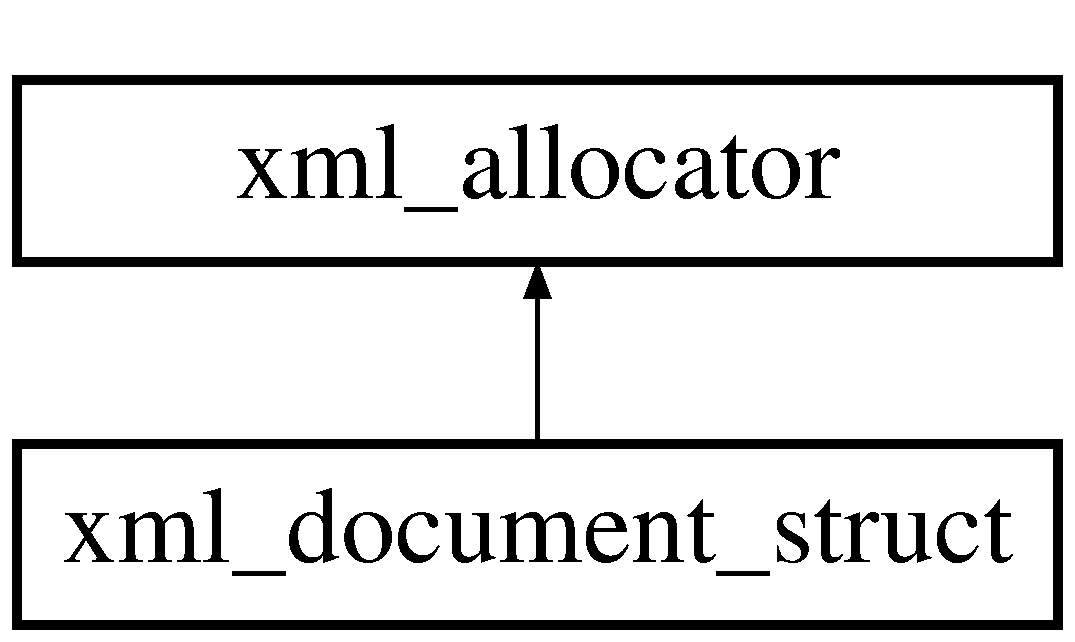
\includegraphics[height=2.000000cm]{structxml__allocator}
\end{center}
\end{figure}
\subsection*{Public Member Functions}
\begin{DoxyCompactItemize}
\item 
\hyperlink{structxml__allocator_ad41b1a18595953aa71a470b45921c0fd}{xml\-\_\-allocator} (\hyperlink{structxml__memory__page}{xml\-\_\-memory\-\_\-page} $\ast$root)
\item 
\hyperlink{structxml__memory__page}{xml\-\_\-memory\-\_\-page} $\ast$ \hyperlink{structxml__allocator_a4b399b01e530220ec5849b912b84063b}{allocate\-\_\-page} (size\-\_\-t data\-\_\-size)
\item 
void $\ast$ \hyperlink{structxml__allocator_a30bb557bc040de54c041c6d3dca6772e}{allocate\-\_\-memory\-\_\-oob} (size\-\_\-t size, \hyperlink{structxml__memory__page}{xml\-\_\-memory\-\_\-page} $\ast$\&out\-\_\-page)
\item 
void $\ast$ \hyperlink{structxml__allocator_afac0b9fac2c2962972f60d0346eb4f39}{allocate\-\_\-memory} (size\-\_\-t size, \hyperlink{structxml__memory__page}{xml\-\_\-memory\-\_\-page} $\ast$\&out\-\_\-page)
\item 
void \hyperlink{structxml__allocator_a5df417155487cce4e0460b123ac33dc6}{deallocate\-\_\-memory} (void $\ast$ptr, size\-\_\-t size, \hyperlink{structxml__memory__page}{xml\-\_\-memory\-\_\-page} $\ast$page)
\item 
char\-\_\-t $\ast$ \hyperlink{structxml__allocator_ac5ec2b5d41672d6494a2742e95e525b3}{allocate\-\_\-string} (size\-\_\-t length)
\item 
void \hyperlink{structxml__allocator_af32c538db4d562c2d0bfe15f7c0aa879}{deallocate\-\_\-string} (char\-\_\-t $\ast$string)
\end{DoxyCompactItemize}
\subsection*{Static Public Member Functions}
\begin{DoxyCompactItemize}
\item 
static void \hyperlink{structxml__allocator_a1c6bfe15a257a094f55659f8d71c209e}{deallocate\-\_\-page} (\hyperlink{structxml__memory__page}{xml\-\_\-memory\-\_\-page} $\ast$page)
\end{DoxyCompactItemize}
\subsection*{Data Fields}
\begin{DoxyCompactItemize}
\item 
\hyperlink{structxml__memory__page}{xml\-\_\-memory\-\_\-page} $\ast$ \hyperlink{structxml__allocator_a38082e85b23743620a257f997a00bb69}{\-\_\-root}
\item 
size\-\_\-t \hyperlink{structxml__allocator_a4908b4aaa8cbbc3bf936ab8a938053c0}{\-\_\-busy\-\_\-size}
\end{DoxyCompactItemize}


\subsection{Constructor \& Destructor Documentation}
\hypertarget{structxml__allocator_ad41b1a18595953aa71a470b45921c0fd}{\index{xml\-\_\-allocator@{xml\-\_\-allocator}!xml\-\_\-allocator@{xml\-\_\-allocator}}
\index{xml\-\_\-allocator@{xml\-\_\-allocator}!xml_allocator@{xml\-\_\-allocator}}
\subsubsection[{xml\-\_\-allocator}]{\setlength{\rightskip}{0pt plus 5cm}xml\-\_\-allocator\-::xml\-\_\-allocator (
\begin{DoxyParamCaption}
\item[{{\bf xml\-\_\-memory\-\_\-page} $\ast$}]{root}
\end{DoxyParamCaption}
)\hspace{0.3cm}{\ttfamily [inline]}}}\label{structxml__allocator_ad41b1a18595953aa71a470b45921c0fd}

\begin{DoxyCode}
292                                             : \hyperlink{structxml__allocator_a38082e85b23743620a257f997a00bb69}{\_root}(root), \hyperlink{structxml__allocator_a4908b4aaa8cbbc3bf936ab8a938053c0}{\_busy\_size}(root->
      \hyperlink{structxml__memory__page_a04780ddabc14b45baba3d1ded79d355a}{busy\_size})
293         \{
294         \}
\end{DoxyCode}


\subsection{Member Function Documentation}
\hypertarget{structxml__allocator_afac0b9fac2c2962972f60d0346eb4f39}{\index{xml\-\_\-allocator@{xml\-\_\-allocator}!allocate\-\_\-memory@{allocate\-\_\-memory}}
\index{allocate\-\_\-memory@{allocate\-\_\-memory}!xml_allocator@{xml\-\_\-allocator}}
\subsubsection[{allocate\-\_\-memory}]{\setlength{\rightskip}{0pt plus 5cm}void$\ast$ xml\-\_\-allocator\-::allocate\-\_\-memory (
\begin{DoxyParamCaption}
\item[{size\-\_\-t}]{size, }
\item[{{\bf xml\-\_\-memory\-\_\-page} $\ast$\&}]{out\-\_\-page}
\end{DoxyParamCaption}
)\hspace{0.3cm}{\ttfamily [inline]}}}\label{structxml__allocator_afac0b9fac2c2962972f60d0346eb4f39}

\begin{DoxyCode}
324         \{
325             \textcolor{keywordflow}{if} (\hyperlink{structxml__allocator_a4908b4aaa8cbbc3bf936ab8a938053c0}{\_busy\_size} + size > xml\_memory\_page\_size) \textcolor{keywordflow}{return} 
      \hyperlink{structxml__allocator_a30bb557bc040de54c041c6d3dca6772e}{allocate\_memory\_oob}(size, out\_page);
326 
327             \textcolor{keywordtype}{void}* buf = \hyperlink{structxml__allocator_a38082e85b23743620a257f997a00bb69}{\_root}->\hyperlink{structxml__memory__page_abd99ed1563aa66fb3573a9208452685c}{data} + \hyperlink{structxml__allocator_a4908b4aaa8cbbc3bf936ab8a938053c0}{\_busy\_size};
328 
329             \hyperlink{structxml__allocator_a4908b4aaa8cbbc3bf936ab8a938053c0}{\_busy\_size} += size;
330 
331             out\_page = \hyperlink{structxml__allocator_a38082e85b23743620a257f997a00bb69}{\_root};
332 
333             \textcolor{keywordflow}{return} buf;
334         \}
\end{DoxyCode}
\hypertarget{structxml__allocator_a30bb557bc040de54c041c6d3dca6772e}{\index{xml\-\_\-allocator@{xml\-\_\-allocator}!allocate\-\_\-memory\-\_\-oob@{allocate\-\_\-memory\-\_\-oob}}
\index{allocate\-\_\-memory\-\_\-oob@{allocate\-\_\-memory\-\_\-oob}!xml_allocator@{xml\-\_\-allocator}}
\subsubsection[{allocate\-\_\-memory\-\_\-oob}]{\setlength{\rightskip}{0pt plus 5cm}{\bf P\-U\-G\-I\-\_\-\-\_\-\-F\-N\-\_\-\-N\-O\-\_\-\-I\-N\-L\-I\-N\-E} void $\ast$ xml\-\_\-allocator\-::allocate\-\_\-memory\-\_\-oob (
\begin{DoxyParamCaption}
\item[{size\-\_\-t}]{size, }
\item[{{\bf xml\-\_\-memory\-\_\-page} $\ast$\&}]{out\-\_\-page}
\end{DoxyParamCaption}
)}}\label{structxml__allocator_a30bb557bc040de54c041c6d3dca6772e}

\begin{DoxyCode}
422     \{
423         \textcolor{keyword}{const} \textcolor{keywordtype}{size\_t} large\_allocation\_threshold = xml\_memory\_page\_size / 4;
424 
425         \hyperlink{structxml__memory__page}{xml\_memory\_page}* page = \hyperlink{structxml__allocator_a4b399b01e530220ec5849b912b84063b}{allocate\_page}(size <= 
      large\_allocation\_threshold ? xml\_memory\_page\_size : size);
426         out\_page = page;
427 
428         \textcolor{keywordflow}{if} (!page) \textcolor{keywordflow}{return} 0;
429 
430         \textcolor{keywordflow}{if} (size <= large\_allocation\_threshold)
431         \{
432             \hyperlink{structxml__allocator_a38082e85b23743620a257f997a00bb69}{\_root}->\hyperlink{structxml__memory__page_a04780ddabc14b45baba3d1ded79d355a}{busy\_size} = \hyperlink{structxml__allocator_a4908b4aaa8cbbc3bf936ab8a938053c0}{\_busy\_size};
433 
434             \textcolor{comment}{// insert page at the end of linked list}
435             page->\hyperlink{structxml__memory__page_a014969b0e4a34a6cb24e9823791e60ab}{prev} = \hyperlink{structxml__allocator_a38082e85b23743620a257f997a00bb69}{\_root};
436             \hyperlink{structxml__allocator_a38082e85b23743620a257f997a00bb69}{\_root}->\hyperlink{structxml__memory__page_a326a74e009af80219ea31bc65ed9e45e}{next} = page;
437             \hyperlink{structxml__allocator_a38082e85b23743620a257f997a00bb69}{\_root} = page;
438 
439             \hyperlink{structxml__allocator_a4908b4aaa8cbbc3bf936ab8a938053c0}{\_busy\_size} = size;
440         \}
441         \textcolor{keywordflow}{else}
442         \{
443             \textcolor{comment}{// insert page before the end of linked list, so that it is deleted as soon as possible}
444             \textcolor{comment}{// the last page is not deleted even if it's empty (see deallocate\_memory)}
445             assert(\hyperlink{structxml__allocator_a38082e85b23743620a257f997a00bb69}{\_root}->\hyperlink{structxml__memory__page_a014969b0e4a34a6cb24e9823791e60ab}{prev});
446 
447             page->\hyperlink{structxml__memory__page_a014969b0e4a34a6cb24e9823791e60ab}{prev} = \hyperlink{structxml__allocator_a38082e85b23743620a257f997a00bb69}{\_root}->\hyperlink{structxml__memory__page_a014969b0e4a34a6cb24e9823791e60ab}{prev};
448             page->\hyperlink{structxml__memory__page_a326a74e009af80219ea31bc65ed9e45e}{next} = \hyperlink{structxml__allocator_a38082e85b23743620a257f997a00bb69}{\_root};
449 
450             \hyperlink{structxml__allocator_a38082e85b23743620a257f997a00bb69}{\_root}->\hyperlink{structxml__memory__page_a014969b0e4a34a6cb24e9823791e60ab}{prev}->\hyperlink{structxml__memory__page_a326a74e009af80219ea31bc65ed9e45e}{next} = page;
451             \hyperlink{structxml__allocator_a38082e85b23743620a257f997a00bb69}{\_root}->\hyperlink{structxml__memory__page_a014969b0e4a34a6cb24e9823791e60ab}{prev} = page;
452         \}
453 
454         \textcolor{comment}{// allocate inside page}
455         page->\hyperlink{structxml__memory__page_a04780ddabc14b45baba3d1ded79d355a}{busy\_size} = size;
456 
457         \textcolor{keywordflow}{return} page->\hyperlink{structxml__memory__page_abd99ed1563aa66fb3573a9208452685c}{data};
458     \}
\end{DoxyCode}
\hypertarget{structxml__allocator_a4b399b01e530220ec5849b912b84063b}{\index{xml\-\_\-allocator@{xml\-\_\-allocator}!allocate\-\_\-page@{allocate\-\_\-page}}
\index{allocate\-\_\-page@{allocate\-\_\-page}!xml_allocator@{xml\-\_\-allocator}}
\subsubsection[{allocate\-\_\-page}]{\setlength{\rightskip}{0pt plus 5cm}{\bf xml\-\_\-memory\-\_\-page}$\ast$ xml\-\_\-allocator\-::allocate\-\_\-page (
\begin{DoxyParamCaption}
\item[{size\-\_\-t}]{data\-\_\-size}
\end{DoxyParamCaption}
)\hspace{0.3cm}{\ttfamily [inline]}}}\label{structxml__allocator_a4b399b01e530220ec5849b912b84063b}

\begin{DoxyCode}
297         \{
298             \textcolor{keywordtype}{size\_t} size = offsetof(\hyperlink{structxml__memory__page}{xml\_memory\_page}, data) + data\_size;
299 
300             \textcolor{comment}{// allocate block with some alignment, leaving memory for worst-case padding}
301             \textcolor{keywordtype}{void}* memory = \hyperlink{structxml__memory__management__function__storage_abb6865f8d07d27fd9273737c59f6e941}{xml\_memory::allocate}(size + xml\_memory\_page\_alignment);
302             \textcolor{keywordflow}{if} (!memory) \textcolor{keywordflow}{return} 0;
303 
304             \textcolor{comment}{// align upwards to page boundary}
305             \textcolor{keywordtype}{void}* page\_memory = \textcolor{keyword}{reinterpret\_cast<}\textcolor{keywordtype}{void}*\textcolor{keyword}{>}((\textcolor{keyword}{reinterpret\_cast<}uintptr\_t\textcolor{keyword}{>}(memory) + (
      xml\_memory\_page\_alignment - 1)) & ~(xml\_memory\_page\_alignment - 1));
306 
307             \textcolor{comment}{// prepare page structure}
308             \hyperlink{structxml__memory__page}{xml\_memory\_page}* page = \hyperlink{structxml__memory__page_ab425973f2abb4fa98ff077d88c0df11c}{xml\_memory\_page::construct}(
      page\_memory);
309 
310             page->\hyperlink{structxml__memory__page_ab51315db80e7f2a5afb87c56fedcd734}{memory} = memory;
311             page->\hyperlink{structxml__memory__page_adf8fa143123a842baa59b82fc3d83c3b}{allocator} = \hyperlink{structxml__allocator_a38082e85b23743620a257f997a00bb69}{\_root}->\hyperlink{structxml__memory__page_adf8fa143123a842baa59b82fc3d83c3b}{allocator};
312 
313             \textcolor{keywordflow}{return} page;
314         \}
\end{DoxyCode}
\hypertarget{structxml__allocator_ac5ec2b5d41672d6494a2742e95e525b3}{\index{xml\-\_\-allocator@{xml\-\_\-allocator}!allocate\-\_\-string@{allocate\-\_\-string}}
\index{allocate\-\_\-string@{allocate\-\_\-string}!xml_allocator@{xml\-\_\-allocator}}
\subsubsection[{allocate\-\_\-string}]{\setlength{\rightskip}{0pt plus 5cm}char\-\_\-t$\ast$ xml\-\_\-allocator\-::allocate\-\_\-string (
\begin{DoxyParamCaption}
\item[{size\-\_\-t}]{length}
\end{DoxyParamCaption}
)\hspace{0.3cm}{\ttfamily [inline]}}}\label{structxml__allocator_ac5ec2b5d41672d6494a2742e95e525b3}

\begin{DoxyCode}
372         \{
373             \textcolor{comment}{// allocate memory for string and header block}
374             \textcolor{keywordtype}{size\_t} size = \textcolor{keyword}{sizeof}(\hyperlink{structxml__memory__string__header}{xml\_memory\_string\_header}) + length * \textcolor{keyword}{sizeof}(
      \hyperlink{namespacepugi_aef5a7a62cba0507542220ea15afe39df}{char\_t});
375             
376             \textcolor{comment}{// round size up to pointer alignment boundary}
377             \textcolor{keywordtype}{size\_t} full\_size = (size + (\textcolor{keyword}{sizeof}(\textcolor{keywordtype}{void}*) - 1)) & ~(\textcolor{keyword}{sizeof}(\textcolor{keywordtype}{void}*) - 1);
378 
379             \hyperlink{structxml__memory__page}{xml\_memory\_page}* page;
380             \hyperlink{structxml__memory__string__header}{xml\_memory\_string\_header}* header = \textcolor{keyword}{static\_cast<}
      \hyperlink{structxml__memory__string__header}{xml\_memory\_string\_header}*\textcolor{keyword}{>}(\hyperlink{structxml__allocator_afac0b9fac2c2962972f60d0346eb4f39}{allocate\_memory}(full\_size, page));
381 
382             \textcolor{keywordflow}{if} (!header) \textcolor{keywordflow}{return} 0;
383 
384             \textcolor{comment}{// setup header}
385             ptrdiff\_t page\_offset = \textcolor{keyword}{reinterpret\_cast<}\textcolor{keywordtype}{char}*\textcolor{keyword}{>}(header) - page->\hyperlink{structxml__memory__page_abd99ed1563aa66fb3573a9208452685c}{data};
386 
387             assert(page\_offset >= 0 && page\_offset < (1 << 16));
388             header->\hyperlink{structxml__memory__string__header_a0cc274672f1263f73eeb6bf839bf96ee}{page\_offset} = \textcolor{keyword}{static\_cast<}uint16\_t\textcolor{keyword}{>}(page\_offset);
389 
390             \textcolor{comment}{// full\_size == 0 for large strings that occupy the whole page}
391             assert(full\_size < (1 << 16) || (page->\hyperlink{structxml__memory__page_a04780ddabc14b45baba3d1ded79d355a}{busy\_size} == full\_size && page\_offset == 0));
392             header->\hyperlink{structxml__memory__string__header_abbb48a709081e6610dffad322499e3f7}{full\_size} = \textcolor{keyword}{static\_cast<}uint16\_t\textcolor{keyword}{>}(full\_size < (1 << 16) ? full\_size : 0);
393 
394             \textcolor{comment}{// round-trip through void* to avoid 'cast increases required alignment of target type' warning}
395             \textcolor{comment}{// header is guaranteed a pointer-sized alignment, which should be enough for char\_t}
396             \textcolor{keywordflow}{return} \textcolor{keyword}{static\_cast<}\hyperlink{namespacepugi_aef5a7a62cba0507542220ea15afe39df}{char\_t}*\textcolor{keyword}{>}(\textcolor{keyword}{static\_cast<}\textcolor{keywordtype}{void}*\textcolor{keyword}{>}(header + 1));
397         \}
\end{DoxyCode}
\hypertarget{structxml__allocator_a5df417155487cce4e0460b123ac33dc6}{\index{xml\-\_\-allocator@{xml\-\_\-allocator}!deallocate\-\_\-memory@{deallocate\-\_\-memory}}
\index{deallocate\-\_\-memory@{deallocate\-\_\-memory}!xml_allocator@{xml\-\_\-allocator}}
\subsubsection[{deallocate\-\_\-memory}]{\setlength{\rightskip}{0pt plus 5cm}void xml\-\_\-allocator\-::deallocate\-\_\-memory (
\begin{DoxyParamCaption}
\item[{void $\ast$}]{ptr, }
\item[{size\-\_\-t}]{size, }
\item[{{\bf xml\-\_\-memory\-\_\-page} $\ast$}]{page}
\end{DoxyParamCaption}
)\hspace{0.3cm}{\ttfamily [inline]}}}\label{structxml__allocator_a5df417155487cce4e0460b123ac33dc6}

\begin{DoxyCode}
337         \{
338             \textcolor{keywordflow}{if} (page == \hyperlink{structxml__allocator_a38082e85b23743620a257f997a00bb69}{\_root}) page->\hyperlink{structxml__memory__page_a04780ddabc14b45baba3d1ded79d355a}{busy\_size} = \hyperlink{structxml__allocator_a4908b4aaa8cbbc3bf936ab8a938053c0}{\_busy\_size};
339 
340             assert(ptr >= page->\hyperlink{structxml__memory__page_abd99ed1563aa66fb3573a9208452685c}{data} && ptr < page->data + page->\hyperlink{structxml__memory__page_a04780ddabc14b45baba3d1ded79d355a}{busy\_size});
341             (void)!ptr;
342 
343             page->\hyperlink{structxml__memory__page_ab4c29645546530a0e1938b53979890a8}{freed\_size} += size;
344             assert(page->\hyperlink{structxml__memory__page_ab4c29645546530a0e1938b53979890a8}{freed\_size} <= page->\hyperlink{structxml__memory__page_a04780ddabc14b45baba3d1ded79d355a}{busy\_size});
345 
346             \textcolor{keywordflow}{if} (page->\hyperlink{structxml__memory__page_ab4c29645546530a0e1938b53979890a8}{freed\_size} == page->\hyperlink{structxml__memory__page_a04780ddabc14b45baba3d1ded79d355a}{busy\_size})
347             \{
348                 \textcolor{keywordflow}{if} (page->\hyperlink{structxml__memory__page_a326a74e009af80219ea31bc65ed9e45e}{next} == 0)
349                 \{
350                     assert(\hyperlink{structxml__allocator_a38082e85b23743620a257f997a00bb69}{\_root} == page);
351 
352                     \textcolor{comment}{// top page freed, just reset sizes}
353                     page->\hyperlink{structxml__memory__page_a04780ddabc14b45baba3d1ded79d355a}{busy\_size} = page->\hyperlink{structxml__memory__page_ab4c29645546530a0e1938b53979890a8}{freed\_size} = 0;
354                     \hyperlink{structxml__allocator_a4908b4aaa8cbbc3bf936ab8a938053c0}{\_busy\_size} = 0;
355                 \}
356                 \textcolor{keywordflow}{else}
357                 \{
358                     assert(\hyperlink{structxml__allocator_a38082e85b23743620a257f997a00bb69}{\_root} != page);
359                     assert(page->\hyperlink{structxml__memory__page_a014969b0e4a34a6cb24e9823791e60ab}{prev});
360 
361                     \textcolor{comment}{// remove from the list}
362                     page->\hyperlink{structxml__memory__page_a014969b0e4a34a6cb24e9823791e60ab}{prev}->\hyperlink{structxml__memory__page_a326a74e009af80219ea31bc65ed9e45e}{next} = page->\hyperlink{structxml__memory__page_a326a74e009af80219ea31bc65ed9e45e}{next};
363                     page->\hyperlink{structxml__memory__page_a326a74e009af80219ea31bc65ed9e45e}{next}->\hyperlink{structxml__memory__page_a014969b0e4a34a6cb24e9823791e60ab}{prev} = page->\hyperlink{structxml__memory__page_a014969b0e4a34a6cb24e9823791e60ab}{prev};
364 
365                     \textcolor{comment}{// deallocate}
366                     \hyperlink{structxml__allocator_a1c6bfe15a257a094f55659f8d71c209e}{deallocate\_page}(page);
367                 \}
368             \}
369         \}
\end{DoxyCode}
\hypertarget{structxml__allocator_a1c6bfe15a257a094f55659f8d71c209e}{\index{xml\-\_\-allocator@{xml\-\_\-allocator}!deallocate\-\_\-page@{deallocate\-\_\-page}}
\index{deallocate\-\_\-page@{deallocate\-\_\-page}!xml_allocator@{xml\-\_\-allocator}}
\subsubsection[{deallocate\-\_\-page}]{\setlength{\rightskip}{0pt plus 5cm}static void xml\-\_\-allocator\-::deallocate\-\_\-page (
\begin{DoxyParamCaption}
\item[{{\bf xml\-\_\-memory\-\_\-page} $\ast$}]{page}
\end{DoxyParamCaption}
)\hspace{0.3cm}{\ttfamily [inline]}, {\ttfamily [static]}}}\label{structxml__allocator_a1c6bfe15a257a094f55659f8d71c209e}

\begin{DoxyCode}
317         \{
318             \hyperlink{structxml__memory__management__function__storage_a1c80a9a045ed6cfb90b17a178e4b3512}{xml\_memory::deallocate}(page->\hyperlink{structxml__memory__page_ab51315db80e7f2a5afb87c56fedcd734}{memory});
319         \}
\end{DoxyCode}
\hypertarget{structxml__allocator_af32c538db4d562c2d0bfe15f7c0aa879}{\index{xml\-\_\-allocator@{xml\-\_\-allocator}!deallocate\-\_\-string@{deallocate\-\_\-string}}
\index{deallocate\-\_\-string@{deallocate\-\_\-string}!xml_allocator@{xml\-\_\-allocator}}
\subsubsection[{deallocate\-\_\-string}]{\setlength{\rightskip}{0pt plus 5cm}void xml\-\_\-allocator\-::deallocate\-\_\-string (
\begin{DoxyParamCaption}
\item[{char\-\_\-t $\ast$}]{string}
\end{DoxyParamCaption}
)\hspace{0.3cm}{\ttfamily [inline]}}}\label{structxml__allocator_af32c538db4d562c2d0bfe15f7c0aa879}

\begin{DoxyCode}
400         \{
401             \textcolor{comment}{// this function casts pointers through void* to avoid 'cast increases required alignment of
       target type' warnings}
402             \textcolor{comment}{// we're guaranteed the proper (pointer-sized) alignment on the input string if it was
       allocated via allocate\_string}
403 
404             \textcolor{comment}{// get header}
405             \hyperlink{structxml__memory__string__header}{xml\_memory\_string\_header}* header = \textcolor{keyword}{static\_cast<}
      \hyperlink{structxml__memory__string__header}{xml\_memory\_string\_header}*\textcolor{keyword}{>}(\textcolor{keyword}{static\_cast<}\textcolor{keywordtype}{void}*\textcolor{keyword}{>}(string)) - 1;
406 
407             \textcolor{comment}{// deallocate}
408             \textcolor{keywordtype}{size\_t} page\_offset = offsetof(\hyperlink{structxml__memory__page}{xml\_memory\_page}, data) + header->
      \hyperlink{structxml__memory__string__header_a0cc274672f1263f73eeb6bf839bf96ee}{page\_offset};
409             \hyperlink{structxml__memory__page}{xml\_memory\_page}* page = \textcolor{keyword}{reinterpret\_cast<}
      \hyperlink{structxml__memory__page}{xml\_memory\_page}*\textcolor{keyword}{>}(\textcolor{keyword}{static\_cast<}\textcolor{keywordtype}{void}*\textcolor{keyword}{>}(\textcolor{keyword}{reinterpret\_cast<}\textcolor{keywordtype}{char}*\textcolor{keyword}{>}(header) - page\_offset));
410 
411             \textcolor{comment}{// if full\_size == 0 then this string occupies the whole page}
412             \textcolor{keywordtype}{size\_t} full\_size = header->\hyperlink{structxml__memory__string__header_abbb48a709081e6610dffad322499e3f7}{full\_size} == 0 ? page->\hyperlink{structxml__memory__page_a04780ddabc14b45baba3d1ded79d355a}{busy\_size} : header->
      \hyperlink{structxml__memory__string__header_abbb48a709081e6610dffad322499e3f7}{full\_size};
413 
414             \hyperlink{structxml__allocator_a5df417155487cce4e0460b123ac33dc6}{deallocate\_memory}(header, full\_size, page);
415         \}
\end{DoxyCode}


\subsection{Field Documentation}
\hypertarget{structxml__allocator_a4908b4aaa8cbbc3bf936ab8a938053c0}{\index{xml\-\_\-allocator@{xml\-\_\-allocator}!\-\_\-busy\-\_\-size@{\-\_\-busy\-\_\-size}}
\index{\-\_\-busy\-\_\-size@{\-\_\-busy\-\_\-size}!xml_allocator@{xml\-\_\-allocator}}
\subsubsection[{\-\_\-busy\-\_\-size}]{\setlength{\rightskip}{0pt plus 5cm}size\-\_\-t xml\-\_\-allocator\-::\-\_\-busy\-\_\-size}}\label{structxml__allocator_a4908b4aaa8cbbc3bf936ab8a938053c0}
\hypertarget{structxml__allocator_a38082e85b23743620a257f997a00bb69}{\index{xml\-\_\-allocator@{xml\-\_\-allocator}!\-\_\-root@{\-\_\-root}}
\index{\-\_\-root@{\-\_\-root}!xml_allocator@{xml\-\_\-allocator}}
\subsubsection[{\-\_\-root}]{\setlength{\rightskip}{0pt plus 5cm}{\bf xml\-\_\-memory\-\_\-page}$\ast$ xml\-\_\-allocator\-::\-\_\-root}}\label{structxml__allocator_a38082e85b23743620a257f997a00bb69}


The documentation for this struct was generated from the following file\-:\begin{DoxyCompactItemize}
\item 
Third\-Party/pugixml/\hyperlink{pugixml_8cpp}{pugixml.\-cpp}\end{DoxyCompactItemize}

\hypertarget{classpugi_1_1xml__attribute}{\section{pugi\-:\-:xml\-\_\-attribute Class Reference}
\label{classpugi_1_1xml__attribute}\index{pugi\-::xml\-\_\-attribute@{pugi\-::xml\-\_\-attribute}}
}


{\ttfamily \#include $<$pugixml.\-hpp$>$}

\subsection*{Public Member Functions}
\begin{DoxyCompactItemize}
\item 
\hyperlink{classpugi_1_1xml__attribute_a03b24e1dfc445e8cb490cbb5b67dca9f}{xml\-\_\-attribute} ()
\item 
\hyperlink{classpugi_1_1xml__attribute_a32b0c063842c2073445cd8c89f1c0db2}{xml\-\_\-attribute} (\hyperlink{structpugi_1_1xml__attribute__struct}{xml\-\_\-attribute\-\_\-struct} $\ast$attr)
\item 
\hyperlink{classpugi_1_1xml__attribute_a108510c1375f1317b7ddb7d4bc15b707}{operator unspecified\-\_\-bool\-\_\-type} () const 
\item 
bool \hyperlink{classpugi_1_1xml__attribute_a0425c1b376c41d71f71416db9b1e1e6b}{operator!} () const 
\item 
bool \hyperlink{classpugi_1_1xml__attribute_ac1ab6dfce7d2a7aa0a6a24c7b84f0a5e}{operator==} (const \hyperlink{classpugi_1_1xml__attribute}{xml\-\_\-attribute} \&r) const 
\item 
bool \hyperlink{classpugi_1_1xml__attribute_a76b57111453b0873b0065fe3c2fe386d}{operator!=} (const \hyperlink{classpugi_1_1xml__attribute}{xml\-\_\-attribute} \&r) const 
\item 
bool \hyperlink{classpugi_1_1xml__attribute_ab887d475d793b4740e53e69b9f908af6}{operator$<$} (const \hyperlink{classpugi_1_1xml__attribute}{xml\-\_\-attribute} \&r) const 
\item 
bool \hyperlink{classpugi_1_1xml__attribute_a11ab6168bb3df31dd23956cc5bd0b871}{operator$>$} (const \hyperlink{classpugi_1_1xml__attribute}{xml\-\_\-attribute} \&r) const 
\item 
bool \hyperlink{classpugi_1_1xml__attribute_ae45e069db2452f535c349c5a605c90e6}{operator$<$=} (const \hyperlink{classpugi_1_1xml__attribute}{xml\-\_\-attribute} \&r) const 
\item 
bool \hyperlink{classpugi_1_1xml__attribute_afaff39714d8bd51f537f372d299d68cd}{operator$>$=} (const \hyperlink{classpugi_1_1xml__attribute}{xml\-\_\-attribute} \&r) const 
\item 
bool \hyperlink{classpugi_1_1xml__attribute_a961a571d7397e1803c3f63cf96052c53}{empty} () const 
\item 
const \hyperlink{namespacepugi_aef5a7a62cba0507542220ea15afe39df}{char\-\_\-t} $\ast$ \hyperlink{classpugi_1_1xml__attribute_a98377c82f36c74f211d16db275577334}{name} () const 
\item 
const \hyperlink{namespacepugi_aef5a7a62cba0507542220ea15afe39df}{char\-\_\-t} $\ast$ \hyperlink{classpugi_1_1xml__attribute_ad535b73777f3eaa1c0c0a3c168683bd3}{value} () const 
\item 
const \hyperlink{namespacepugi_aef5a7a62cba0507542220ea15afe39df}{char\-\_\-t} $\ast$ \hyperlink{classpugi_1_1xml__attribute_a583f470d768f5f8a4df0ebb2e016a88d}{as\-\_\-string} (const \hyperlink{namespacepugi_aef5a7a62cba0507542220ea15afe39df}{char\-\_\-t} $\ast$def=\hyperlink{pugixml_8hpp_ad5475bca2e336810ae5906349e644d0b}{P\-U\-G\-I\-X\-M\-L\-\_\-\-T\-E\-X\-T}(\char`\"{}\char`\"{})) const 
\item 
int \hyperlink{classpugi_1_1xml__attribute_afe009e964b9cec96c77495ef1ae6d91f}{as\-\_\-int} (int def=0) const 
\item 
unsigned int \hyperlink{classpugi_1_1xml__attribute_af89be4951cf7567053bcbb66ce013156}{as\-\_\-uint} (unsigned int def=0) const 
\item 
double \hyperlink{classpugi_1_1xml__attribute_acd8d510ac7825b0f52f4795d2cc5e00b}{as\-\_\-double} (double def=0) const 
\item 
float \hyperlink{classpugi_1_1xml__attribute_a23f960683dba03f32ed4da19a10c769d}{as\-\_\-float} (float def=0) const 
\item 
bool \hyperlink{classpugi_1_1xml__attribute_a715646ddcfcd9f327934f9083f949796}{as\-\_\-bool} (bool def=false) const 
\item 
bool \hyperlink{classpugi_1_1xml__attribute_ae8ffb5ef48338f27015337a6f57b6595}{set\-\_\-name} (const \hyperlink{namespacepugi_aef5a7a62cba0507542220ea15afe39df}{char\-\_\-t} $\ast$rhs)
\item 
bool \hyperlink{classpugi_1_1xml__attribute_af2ca1f0d13ee8f661bc17524bedc13d7}{set\-\_\-value} (const \hyperlink{namespacepugi_aef5a7a62cba0507542220ea15afe39df}{char\-\_\-t} $\ast$rhs)
\item 
bool \hyperlink{classpugi_1_1xml__attribute_aa9fcffccebda6ae6169e4d17265bd39a}{set\-\_\-value} (int rhs)
\item 
bool \hyperlink{classpugi_1_1xml__attribute_abffdc566e5e2805c493f18f8424f5024}{set\-\_\-value} (unsigned int rhs)
\item 
bool \hyperlink{classpugi_1_1xml__attribute_a5e58f7565792ba3afd432325f824f1b3}{set\-\_\-value} (double rhs)
\item 
bool \hyperlink{classpugi_1_1xml__attribute_a33ab85a706a18f88241081ab8b0f823f}{set\-\_\-value} (bool rhs)
\item 
\hyperlink{classpugi_1_1xml__attribute}{xml\-\_\-attribute} \& \hyperlink{classpugi_1_1xml__attribute_a957f7613ba25623fa3bdf1c50346b869}{operator=} (const \hyperlink{namespacepugi_aef5a7a62cba0507542220ea15afe39df}{char\-\_\-t} $\ast$rhs)
\item 
\hyperlink{classpugi_1_1xml__attribute}{xml\-\_\-attribute} \& \hyperlink{classpugi_1_1xml__attribute_a15f8f489bf3170dbadf28d4a89b20201}{operator=} (int rhs)
\item 
\hyperlink{classpugi_1_1xml__attribute}{xml\-\_\-attribute} \& \hyperlink{classpugi_1_1xml__attribute_a7f9f6b7ef7456873cc1c4957a806c958}{operator=} (unsigned int rhs)
\item 
\hyperlink{classpugi_1_1xml__attribute}{xml\-\_\-attribute} \& \hyperlink{classpugi_1_1xml__attribute_a4383afaf2e420ed45c563b2b82a3661f}{operator=} (double rhs)
\item 
\hyperlink{classpugi_1_1xml__attribute}{xml\-\_\-attribute} \& \hyperlink{classpugi_1_1xml__attribute_ae23d29ab032d5ff7c875f5bbe4d6ab3c}{operator=} (bool rhs)
\item 
\hyperlink{classpugi_1_1xml__attribute}{xml\-\_\-attribute} \hyperlink{classpugi_1_1xml__attribute_a71b0ee33f833781a94d6d35adfc0daac}{next\-\_\-attribute} () const 
\item 
\hyperlink{classpugi_1_1xml__attribute}{xml\-\_\-attribute} \hyperlink{classpugi_1_1xml__attribute_aee4fc29d1645bddc70f1a174654b9d10}{previous\-\_\-attribute} () const 
\item 
size\-\_\-t \hyperlink{classpugi_1_1xml__attribute_a1c9776e159263d00082a395891d8470f}{hash\-\_\-value} () const 
\item 
\hyperlink{structpugi_1_1xml__attribute__struct}{xml\-\_\-attribute\-\_\-struct} $\ast$ \hyperlink{classpugi_1_1xml__attribute_aa8543b8406bfddd2607c8dcdb54c5369}{internal\-\_\-object} () const 
\end{DoxyCompactItemize}
\subsection*{Friends}
\begin{DoxyCompactItemize}
\item 
class \hyperlink{classpugi_1_1xml__attribute_aeff34dec57ee910e3344631528969539}{xml\-\_\-attribute\-\_\-iterator}
\item 
class \hyperlink{classpugi_1_1xml__attribute_a156d917a92815c7b593bd5ef19f6d5fb}{xml\-\_\-node}
\end{DoxyCompactItemize}


\subsection{Constructor \& Destructor Documentation}
\hypertarget{classpugi_1_1xml__attribute_a03b24e1dfc445e8cb490cbb5b67dca9f}{\index{pugi\-::xml\-\_\-attribute@{pugi\-::xml\-\_\-attribute}!xml\-\_\-attribute@{xml\-\_\-attribute}}
\index{xml\-\_\-attribute@{xml\-\_\-attribute}!pugi::xml_attribute@{pugi\-::xml\-\_\-attribute}}
\subsubsection[{xml\-\_\-attribute}]{\setlength{\rightskip}{0pt plus 5cm}{\bf P\-U\-G\-I\-\_\-\-\_\-\-F\-N} pugi\-::xml\-\_\-attribute\-::xml\-\_\-attribute (
\begin{DoxyParamCaption}
{}
\end{DoxyParamCaption}
)}}\label{classpugi_1_1xml__attribute_a03b24e1dfc445e8cb490cbb5b67dca9f}

\begin{DoxyCode}
3716                                          : \_attr(0)
3717     \{
3718     \}
\end{DoxyCode}
\hypertarget{classpugi_1_1xml__attribute_a32b0c063842c2073445cd8c89f1c0db2}{\index{pugi\-::xml\-\_\-attribute@{pugi\-::xml\-\_\-attribute}!xml\-\_\-attribute@{xml\-\_\-attribute}}
\index{xml\-\_\-attribute@{xml\-\_\-attribute}!pugi::xml_attribute@{pugi\-::xml\-\_\-attribute}}
\subsubsection[{xml\-\_\-attribute}]{\setlength{\rightskip}{0pt plus 5cm}{\bf P\-U\-G\-I\-\_\-\-\_\-\-F\-N} pugi\-::xml\-\_\-attribute\-::xml\-\_\-attribute (
\begin{DoxyParamCaption}
\item[{{\bf xml\-\_\-attribute\-\_\-struct} $\ast$}]{attr}
\end{DoxyParamCaption}
)\hspace{0.3cm}{\ttfamily [explicit]}}}\label{classpugi_1_1xml__attribute_a32b0c063842c2073445cd8c89f1c0db2}

\begin{DoxyCode}
3720                                                                    : \_attr(attr)
3721     \{
3722     \}
\end{DoxyCode}


\subsection{Member Function Documentation}
\hypertarget{classpugi_1_1xml__attribute_a715646ddcfcd9f327934f9083f949796}{\index{pugi\-::xml\-\_\-attribute@{pugi\-::xml\-\_\-attribute}!as\-\_\-bool@{as\-\_\-bool}}
\index{as\-\_\-bool@{as\-\_\-bool}!pugi::xml_attribute@{pugi\-::xml\-\_\-attribute}}
\subsubsection[{as\-\_\-bool}]{\setlength{\rightskip}{0pt plus 5cm}{\bf P\-U\-G\-I\-\_\-\-\_\-\-F\-N} bool pugi\-::xml\-\_\-attribute\-::as\-\_\-bool (
\begin{DoxyParamCaption}
\item[{bool}]{def = {\ttfamily false}}
\end{DoxyParamCaption}
) const}}\label{classpugi_1_1xml__attribute_a715646ddcfcd9f327934f9083f949796}

\begin{DoxyCode}
3804     \{
3805         \textcolor{keywordflow}{return} \hyperlink{pugixml_8cpp_a8458bf6b4828301059456c3ea00e7331}{impl::get\_value\_bool}(\_attr ? \_attr->\hyperlink{structpugi_1_1xml__attribute__struct_ae652627d56cb9dcc0afdd1fbf6570364}{value} : 0, def);
3806     \}
\end{DoxyCode}
\hypertarget{classpugi_1_1xml__attribute_acd8d510ac7825b0f52f4795d2cc5e00b}{\index{pugi\-::xml\-\_\-attribute@{pugi\-::xml\-\_\-attribute}!as\-\_\-double@{as\-\_\-double}}
\index{as\-\_\-double@{as\-\_\-double}!pugi::xml_attribute@{pugi\-::xml\-\_\-attribute}}
\subsubsection[{as\-\_\-double}]{\setlength{\rightskip}{0pt plus 5cm}{\bf P\-U\-G\-I\-\_\-\-\_\-\-F\-N} double pugi\-::xml\-\_\-attribute\-::as\-\_\-double (
\begin{DoxyParamCaption}
\item[{double}]{def = {\ttfamily 0}}
\end{DoxyParamCaption}
) const}}\label{classpugi_1_1xml__attribute_acd8d510ac7825b0f52f4795d2cc5e00b}

\begin{DoxyCode}
3794     \{
3795         \textcolor{keywordflow}{return} \hyperlink{pugixml_8cpp_a89d53cca88a1787eaff695225c52ac9e}{impl::get\_value\_double}(\_attr ? \_attr->\hyperlink{structpugi_1_1xml__attribute__struct_ae652627d56cb9dcc0afdd1fbf6570364}{value} : 0, def);
3796     \}
\end{DoxyCode}
\hypertarget{classpugi_1_1xml__attribute_a23f960683dba03f32ed4da19a10c769d}{\index{pugi\-::xml\-\_\-attribute@{pugi\-::xml\-\_\-attribute}!as\-\_\-float@{as\-\_\-float}}
\index{as\-\_\-float@{as\-\_\-float}!pugi::xml_attribute@{pugi\-::xml\-\_\-attribute}}
\subsubsection[{as\-\_\-float}]{\setlength{\rightskip}{0pt plus 5cm}{\bf P\-U\-G\-I\-\_\-\-\_\-\-F\-N} float pugi\-::xml\-\_\-attribute\-::as\-\_\-float (
\begin{DoxyParamCaption}
\item[{float}]{def = {\ttfamily 0}}
\end{DoxyParamCaption}
) const}}\label{classpugi_1_1xml__attribute_a23f960683dba03f32ed4da19a10c769d}

\begin{DoxyCode}
3799     \{
3800         \textcolor{keywordflow}{return} \hyperlink{pugixml_8cpp_ae8ed6162cf7a98281598daa4d858c757}{impl::get\_value\_float}(\_attr ? \_attr->\hyperlink{structpugi_1_1xml__attribute__struct_ae652627d56cb9dcc0afdd1fbf6570364}{value} : 0, def);
3801     \}
\end{DoxyCode}
\hypertarget{classpugi_1_1xml__attribute_afe009e964b9cec96c77495ef1ae6d91f}{\index{pugi\-::xml\-\_\-attribute@{pugi\-::xml\-\_\-attribute}!as\-\_\-int@{as\-\_\-int}}
\index{as\-\_\-int@{as\-\_\-int}!pugi::xml_attribute@{pugi\-::xml\-\_\-attribute}}
\subsubsection[{as\-\_\-int}]{\setlength{\rightskip}{0pt plus 5cm}{\bf P\-U\-G\-I\-\_\-\-\_\-\-F\-N} int pugi\-::xml\-\_\-attribute\-::as\-\_\-int (
\begin{DoxyParamCaption}
\item[{int}]{def = {\ttfamily 0}}
\end{DoxyParamCaption}
) const}}\label{classpugi_1_1xml__attribute_afe009e964b9cec96c77495ef1ae6d91f}

\begin{DoxyCode}
3784     \{
3785         \textcolor{keywordflow}{return} \hyperlink{pugixml_8cpp_afe79ce7d93b358eb7f503cc5eb7fd7df}{impl::get\_value\_int}(\_attr ? \_attr->\hyperlink{structpugi_1_1xml__attribute__struct_ae652627d56cb9dcc0afdd1fbf6570364}{value} : 0, def);
3786     \}
\end{DoxyCode}
\hypertarget{classpugi_1_1xml__attribute_a583f470d768f5f8a4df0ebb2e016a88d}{\index{pugi\-::xml\-\_\-attribute@{pugi\-::xml\-\_\-attribute}!as\-\_\-string@{as\-\_\-string}}
\index{as\-\_\-string@{as\-\_\-string}!pugi::xml_attribute@{pugi\-::xml\-\_\-attribute}}
\subsubsection[{as\-\_\-string}]{\setlength{\rightskip}{0pt plus 5cm}{\bf P\-U\-G\-I\-\_\-\-\_\-\-F\-N} const {\bf char\-\_\-t} $\ast$ pugi\-::xml\-\_\-attribute\-::as\-\_\-string (
\begin{DoxyParamCaption}
\item[{const {\bf char\-\_\-t} $\ast$}]{def = {\ttfamily {\bf P\-U\-G\-I\-X\-M\-L\-\_\-\-T\-E\-X\-T}(\char`\"{}\char`\"{})}}
\end{DoxyParamCaption}
) const}}\label{classpugi_1_1xml__attribute_a583f470d768f5f8a4df0ebb2e016a88d}

\begin{DoxyCode}
3779     \{
3780         \textcolor{keywordflow}{return} (\_attr && \_attr->\hyperlink{structpugi_1_1xml__attribute__struct_ae652627d56cb9dcc0afdd1fbf6570364}{value}) ? \_attr->\hyperlink{structpugi_1_1xml__attribute__struct_ae652627d56cb9dcc0afdd1fbf6570364}{value} : def;
3781     \}
\end{DoxyCode}
\hypertarget{classpugi_1_1xml__attribute_af89be4951cf7567053bcbb66ce013156}{\index{pugi\-::xml\-\_\-attribute@{pugi\-::xml\-\_\-attribute}!as\-\_\-uint@{as\-\_\-uint}}
\index{as\-\_\-uint@{as\-\_\-uint}!pugi::xml_attribute@{pugi\-::xml\-\_\-attribute}}
\subsubsection[{as\-\_\-uint}]{\setlength{\rightskip}{0pt plus 5cm}{\bf P\-U\-G\-I\-\_\-\-\_\-\-F\-N} unsigned int pugi\-::xml\-\_\-attribute\-::as\-\_\-uint (
\begin{DoxyParamCaption}
\item[{unsigned int}]{def = {\ttfamily 0}}
\end{DoxyParamCaption}
) const}}\label{classpugi_1_1xml__attribute_af89be4951cf7567053bcbb66ce013156}

\begin{DoxyCode}
3789     \{
3790         \textcolor{keywordflow}{return} \hyperlink{pugixml_8cpp_ae610c0c654729981dd58b2d2d19f6f07}{impl::get\_value\_uint}(\_attr ? \_attr->\hyperlink{structpugi_1_1xml__attribute__struct_ae652627d56cb9dcc0afdd1fbf6570364}{value} : 0, def);
3791     \}
\end{DoxyCode}
\hypertarget{classpugi_1_1xml__attribute_a961a571d7397e1803c3f63cf96052c53}{\index{pugi\-::xml\-\_\-attribute@{pugi\-::xml\-\_\-attribute}!empty@{empty}}
\index{empty@{empty}!pugi::xml_attribute@{pugi\-::xml\-\_\-attribute}}
\subsubsection[{empty}]{\setlength{\rightskip}{0pt plus 5cm}{\bf P\-U\-G\-I\-\_\-\-\_\-\-F\-N} bool pugi\-::xml\-\_\-attribute\-::empty (
\begin{DoxyParamCaption}
{}
\end{DoxyParamCaption}
) const}}\label{classpugi_1_1xml__attribute_a961a571d7397e1803c3f63cf96052c53}

\begin{DoxyCode}
3809     \{
3810         \textcolor{keywordflow}{return} !\_attr;
3811     \}
\end{DoxyCode}
\hypertarget{classpugi_1_1xml__attribute_a1c9776e159263d00082a395891d8470f}{\index{pugi\-::xml\-\_\-attribute@{pugi\-::xml\-\_\-attribute}!hash\-\_\-value@{hash\-\_\-value}}
\index{hash\-\_\-value@{hash\-\_\-value}!pugi::xml_attribute@{pugi\-::xml\-\_\-attribute}}
\subsubsection[{hash\-\_\-value}]{\setlength{\rightskip}{0pt plus 5cm}{\bf P\-U\-G\-I\-\_\-\-\_\-\-F\-N} size\-\_\-t pugi\-::xml\-\_\-attribute\-::hash\-\_\-value (
\begin{DoxyParamCaption}
{}
\end{DoxyParamCaption}
) const}}\label{classpugi_1_1xml__attribute_a1c9776e159263d00082a395891d8470f}

\begin{DoxyCode}
3824     \{
3825         \textcolor{keywordflow}{return} \textcolor{keyword}{static\_cast<}\textcolor{keywordtype}{size\_t}\textcolor{keyword}{>}(\textcolor{keyword}{reinterpret\_cast<}uintptr\_t\textcolor{keyword}{>}(\_attr) / \textcolor{keyword}{sizeof}(xml\_attribute\_struct));
3826     \}
\end{DoxyCode}
\hypertarget{classpugi_1_1xml__attribute_aa8543b8406bfddd2607c8dcdb54c5369}{\index{pugi\-::xml\-\_\-attribute@{pugi\-::xml\-\_\-attribute}!internal\-\_\-object@{internal\-\_\-object}}
\index{internal\-\_\-object@{internal\-\_\-object}!pugi::xml_attribute@{pugi\-::xml\-\_\-attribute}}
\subsubsection[{internal\-\_\-object}]{\setlength{\rightskip}{0pt plus 5cm}{\bf P\-U\-G\-I\-\_\-\-\_\-\-F\-N} {\bf xml\-\_\-attribute\-\_\-struct} $\ast$ pugi\-::xml\-\_\-attribute\-::internal\-\_\-object (
\begin{DoxyParamCaption}
{}
\end{DoxyParamCaption}
) const}}\label{classpugi_1_1xml__attribute_aa8543b8406bfddd2607c8dcdb54c5369}

\begin{DoxyCode}
3829     \{
3830         \textcolor{keywordflow}{return} \_attr;
3831     \}
\end{DoxyCode}
\hypertarget{classpugi_1_1xml__attribute_a98377c82f36c74f211d16db275577334}{\index{pugi\-::xml\-\_\-attribute@{pugi\-::xml\-\_\-attribute}!name@{name}}
\index{name@{name}!pugi::xml_attribute@{pugi\-::xml\-\_\-attribute}}
\subsubsection[{name}]{\setlength{\rightskip}{0pt plus 5cm}{\bf P\-U\-G\-I\-\_\-\-\_\-\-F\-N} const {\bf char\-\_\-t} $\ast$ pugi\-::xml\-\_\-attribute\-::name (
\begin{DoxyParamCaption}
{}
\end{DoxyParamCaption}
) const}}\label{classpugi_1_1xml__attribute_a98377c82f36c74f211d16db275577334}

\begin{DoxyCode}
3814     \{
3815         \textcolor{keywordflow}{return} (\_attr && \_attr->\hyperlink{structpugi_1_1xml__attribute__struct_aa886c4aae23a132e1704717721ee2c19}{name}) ? \_attr->\hyperlink{structpugi_1_1xml__attribute__struct_aa886c4aae23a132e1704717721ee2c19}{name} : \hyperlink{pugixml_8hpp_ad5475bca2e336810ae5906349e644d0b}{PUGIXML\_TEXT}(\textcolor{stringliteral}{""});
3816     \}
\end{DoxyCode}
\hypertarget{classpugi_1_1xml__attribute_a71b0ee33f833781a94d6d35adfc0daac}{\index{pugi\-::xml\-\_\-attribute@{pugi\-::xml\-\_\-attribute}!next\-\_\-attribute@{next\-\_\-attribute}}
\index{next\-\_\-attribute@{next\-\_\-attribute}!pugi::xml_attribute@{pugi\-::xml\-\_\-attribute}}
\subsubsection[{next\-\_\-attribute}]{\setlength{\rightskip}{0pt plus 5cm}{\bf P\-U\-G\-I\-\_\-\-\_\-\-F\-N} {\bf xml\-\_\-attribute} pugi\-::xml\-\_\-attribute\-::next\-\_\-attribute (
\begin{DoxyParamCaption}
{}
\end{DoxyParamCaption}
) const}}\label{classpugi_1_1xml__attribute_a71b0ee33f833781a94d6d35adfc0daac}

\begin{DoxyCode}
3769     \{
3770         \textcolor{keywordflow}{return} \_attr ? \hyperlink{classpugi_1_1xml__attribute_a03b24e1dfc445e8cb490cbb5b67dca9f}{xml\_attribute}(\_attr->\hyperlink{structpugi_1_1xml__attribute__struct_a9860c0eb7fa72dc9b69ee9b0575f9efc}{next\_attribute}) : xml\_attribute();
3771     \}
\end{DoxyCode}
\hypertarget{classpugi_1_1xml__attribute_a108510c1375f1317b7ddb7d4bc15b707}{\index{pugi\-::xml\-\_\-attribute@{pugi\-::xml\-\_\-attribute}!operator unspecified\-\_\-bool\-\_\-type@{operator unspecified\-\_\-bool\-\_\-type}}
\index{operator unspecified\-\_\-bool\-\_\-type@{operator unspecified\-\_\-bool\-\_\-type}!pugi::xml_attribute@{pugi\-::xml\-\_\-attribute}}
\subsubsection[{operator unspecified\-\_\-bool\-\_\-type}]{\setlength{\rightskip}{0pt plus 5cm}{\bf P\-U\-G\-I\-\_\-\-\_\-\-F\-N} pugi\-::xml\-\_\-attribute\-::operator xml\-\_\-attribute\-::unspecified\-\_\-bool\-\_\-type (
\begin{DoxyParamCaption}
{}
\end{DoxyParamCaption}
) const}}\label{classpugi_1_1xml__attribute_a108510c1375f1317b7ddb7d4bc15b707}

\begin{DoxyCode}
3729     \{
3730         \textcolor{keywordflow}{return} \_attr ? unspecified\_bool\_xml\_attribute : 0;
3731     \}
\end{DoxyCode}
\hypertarget{classpugi_1_1xml__attribute_a0425c1b376c41d71f71416db9b1e1e6b}{\index{pugi\-::xml\-\_\-attribute@{pugi\-::xml\-\_\-attribute}!operator!@{operator!}}
\index{operator!@{operator!}!pugi::xml_attribute@{pugi\-::xml\-\_\-attribute}}
\subsubsection[{operator!}]{\setlength{\rightskip}{0pt plus 5cm}{\bf P\-U\-G\-I\-\_\-\-\_\-\-F\-N} bool pugi\-::xml\-\_\-attribute\-::operator! (
\begin{DoxyParamCaption}
{}
\end{DoxyParamCaption}
) const}}\label{classpugi_1_1xml__attribute_a0425c1b376c41d71f71416db9b1e1e6b}

\begin{DoxyCode}
3734     \{
3735         \textcolor{keywordflow}{return} !\_attr;
3736     \}
\end{DoxyCode}
\hypertarget{classpugi_1_1xml__attribute_a76b57111453b0873b0065fe3c2fe386d}{\index{pugi\-::xml\-\_\-attribute@{pugi\-::xml\-\_\-attribute}!operator!=@{operator!=}}
\index{operator!=@{operator!=}!pugi::xml_attribute@{pugi\-::xml\-\_\-attribute}}
\subsubsection[{operator!=}]{\setlength{\rightskip}{0pt plus 5cm}{\bf P\-U\-G\-I\-\_\-\-\_\-\-F\-N} bool {\bf pugi\-::xml\-\_\-attribute\-::operator!}= (
\begin{DoxyParamCaption}
\item[{const {\bf xml\-\_\-attribute} \&}]{r}
\end{DoxyParamCaption}
) const}}\label{classpugi_1_1xml__attribute_a76b57111453b0873b0065fe3c2fe386d}

\begin{DoxyCode}
3744     \{
3745         \textcolor{keywordflow}{return} (\_attr != r.\_attr);
3746     \}
\end{DoxyCode}
\hypertarget{classpugi_1_1xml__attribute_ab887d475d793b4740e53e69b9f908af6}{\index{pugi\-::xml\-\_\-attribute@{pugi\-::xml\-\_\-attribute}!operator$<$@{operator$<$}}
\index{operator$<$@{operator$<$}!pugi::xml_attribute@{pugi\-::xml\-\_\-attribute}}
\subsubsection[{operator$<$}]{\setlength{\rightskip}{0pt plus 5cm}{\bf P\-U\-G\-I\-\_\-\-\_\-\-F\-N} bool pugi\-::xml\-\_\-attribute\-::operator$<$ (
\begin{DoxyParamCaption}
\item[{const {\bf xml\-\_\-attribute} \&}]{r}
\end{DoxyParamCaption}
) const}}\label{classpugi_1_1xml__attribute_ab887d475d793b4740e53e69b9f908af6}

\begin{DoxyCode}
3749     \{
3750         \textcolor{keywordflow}{return} (\_attr < r.\_attr);
3751     \}
\end{DoxyCode}
\hypertarget{classpugi_1_1xml__attribute_ae45e069db2452f535c349c5a605c90e6}{\index{pugi\-::xml\-\_\-attribute@{pugi\-::xml\-\_\-attribute}!operator$<$=@{operator$<$=}}
\index{operator$<$=@{operator$<$=}!pugi::xml_attribute@{pugi\-::xml\-\_\-attribute}}
\subsubsection[{operator$<$=}]{\setlength{\rightskip}{0pt plus 5cm}{\bf P\-U\-G\-I\-\_\-\-\_\-\-F\-N} bool pugi\-::xml\-\_\-attribute\-::operator$<$= (
\begin{DoxyParamCaption}
\item[{const {\bf xml\-\_\-attribute} \&}]{r}
\end{DoxyParamCaption}
) const}}\label{classpugi_1_1xml__attribute_ae45e069db2452f535c349c5a605c90e6}

\begin{DoxyCode}
3759     \{
3760         \textcolor{keywordflow}{return} (\_attr <= r.\_attr);
3761     \}
\end{DoxyCode}
\hypertarget{classpugi_1_1xml__attribute_a957f7613ba25623fa3bdf1c50346b869}{\index{pugi\-::xml\-\_\-attribute@{pugi\-::xml\-\_\-attribute}!operator=@{operator=}}
\index{operator=@{operator=}!pugi::xml_attribute@{pugi\-::xml\-\_\-attribute}}
\subsubsection[{operator=}]{\setlength{\rightskip}{0pt plus 5cm}{\bf P\-U\-G\-I\-\_\-\-\_\-\-F\-N} {\bf xml\-\_\-attribute} \& pugi\-::xml\-\_\-attribute\-::operator= (
\begin{DoxyParamCaption}
\item[{const {\bf char\-\_\-t} $\ast$}]{rhs}
\end{DoxyParamCaption}
)}}\label{classpugi_1_1xml__attribute_a957f7613ba25623fa3bdf1c50346b869}

\begin{DoxyCode}
3834     \{
3835         \hyperlink{classpugi_1_1xml__attribute_af2ca1f0d13ee8f661bc17524bedc13d7}{set\_value}(rhs);
3836         \textcolor{keywordflow}{return} *\textcolor{keyword}{this};
3837     \}
\end{DoxyCode}
\hypertarget{classpugi_1_1xml__attribute_a15f8f489bf3170dbadf28d4a89b20201}{\index{pugi\-::xml\-\_\-attribute@{pugi\-::xml\-\_\-attribute}!operator=@{operator=}}
\index{operator=@{operator=}!pugi::xml_attribute@{pugi\-::xml\-\_\-attribute}}
\subsubsection[{operator=}]{\setlength{\rightskip}{0pt plus 5cm}{\bf P\-U\-G\-I\-\_\-\-\_\-\-F\-N} {\bf xml\-\_\-attribute} \& pugi\-::xml\-\_\-attribute\-::operator= (
\begin{DoxyParamCaption}
\item[{int}]{rhs}
\end{DoxyParamCaption}
)}}\label{classpugi_1_1xml__attribute_a15f8f489bf3170dbadf28d4a89b20201}

\begin{DoxyCode}
3840     \{
3841         \hyperlink{classpugi_1_1xml__attribute_af2ca1f0d13ee8f661bc17524bedc13d7}{set\_value}(rhs);
3842         \textcolor{keywordflow}{return} *\textcolor{keyword}{this};
3843     \}
\end{DoxyCode}
\hypertarget{classpugi_1_1xml__attribute_a7f9f6b7ef7456873cc1c4957a806c958}{\index{pugi\-::xml\-\_\-attribute@{pugi\-::xml\-\_\-attribute}!operator=@{operator=}}
\index{operator=@{operator=}!pugi::xml_attribute@{pugi\-::xml\-\_\-attribute}}
\subsubsection[{operator=}]{\setlength{\rightskip}{0pt plus 5cm}{\bf P\-U\-G\-I\-\_\-\-\_\-\-F\-N} {\bf xml\-\_\-attribute} \& pugi\-::xml\-\_\-attribute\-::operator= (
\begin{DoxyParamCaption}
\item[{unsigned int}]{rhs}
\end{DoxyParamCaption}
)}}\label{classpugi_1_1xml__attribute_a7f9f6b7ef7456873cc1c4957a806c958}

\begin{DoxyCode}
3846     \{
3847         \hyperlink{classpugi_1_1xml__attribute_af2ca1f0d13ee8f661bc17524bedc13d7}{set\_value}(rhs);
3848         \textcolor{keywordflow}{return} *\textcolor{keyword}{this};
3849     \}
\end{DoxyCode}
\hypertarget{classpugi_1_1xml__attribute_a4383afaf2e420ed45c563b2b82a3661f}{\index{pugi\-::xml\-\_\-attribute@{pugi\-::xml\-\_\-attribute}!operator=@{operator=}}
\index{operator=@{operator=}!pugi::xml_attribute@{pugi\-::xml\-\_\-attribute}}
\subsubsection[{operator=}]{\setlength{\rightskip}{0pt plus 5cm}{\bf P\-U\-G\-I\-\_\-\-\_\-\-F\-N} {\bf xml\-\_\-attribute} \& pugi\-::xml\-\_\-attribute\-::operator= (
\begin{DoxyParamCaption}
\item[{double}]{rhs}
\end{DoxyParamCaption}
)}}\label{classpugi_1_1xml__attribute_a4383afaf2e420ed45c563b2b82a3661f}

\begin{DoxyCode}
3852     \{
3853         \hyperlink{classpugi_1_1xml__attribute_af2ca1f0d13ee8f661bc17524bedc13d7}{set\_value}(rhs);
3854         \textcolor{keywordflow}{return} *\textcolor{keyword}{this};
3855     \}
\end{DoxyCode}
\hypertarget{classpugi_1_1xml__attribute_ae23d29ab032d5ff7c875f5bbe4d6ab3c}{\index{pugi\-::xml\-\_\-attribute@{pugi\-::xml\-\_\-attribute}!operator=@{operator=}}
\index{operator=@{operator=}!pugi::xml_attribute@{pugi\-::xml\-\_\-attribute}}
\subsubsection[{operator=}]{\setlength{\rightskip}{0pt plus 5cm}{\bf P\-U\-G\-I\-\_\-\-\_\-\-F\-N} {\bf xml\-\_\-attribute} \& pugi\-::xml\-\_\-attribute\-::operator= (
\begin{DoxyParamCaption}
\item[{bool}]{rhs}
\end{DoxyParamCaption}
)}}\label{classpugi_1_1xml__attribute_ae23d29ab032d5ff7c875f5bbe4d6ab3c}

\begin{DoxyCode}
3858     \{
3859         \hyperlink{classpugi_1_1xml__attribute_af2ca1f0d13ee8f661bc17524bedc13d7}{set\_value}(rhs);
3860         \textcolor{keywordflow}{return} *\textcolor{keyword}{this};
3861     \}
\end{DoxyCode}
\hypertarget{classpugi_1_1xml__attribute_ac1ab6dfce7d2a7aa0a6a24c7b84f0a5e}{\index{pugi\-::xml\-\_\-attribute@{pugi\-::xml\-\_\-attribute}!operator==@{operator==}}
\index{operator==@{operator==}!pugi::xml_attribute@{pugi\-::xml\-\_\-attribute}}
\subsubsection[{operator==}]{\setlength{\rightskip}{0pt plus 5cm}{\bf P\-U\-G\-I\-\_\-\-\_\-\-F\-N} bool pugi\-::xml\-\_\-attribute\-::operator== (
\begin{DoxyParamCaption}
\item[{const {\bf xml\-\_\-attribute} \&}]{r}
\end{DoxyParamCaption}
) const}}\label{classpugi_1_1xml__attribute_ac1ab6dfce7d2a7aa0a6a24c7b84f0a5e}

\begin{DoxyCode}
3739     \{
3740         \textcolor{keywordflow}{return} (\_attr == r.\_attr);
3741     \}
\end{DoxyCode}
\hypertarget{classpugi_1_1xml__attribute_a11ab6168bb3df31dd23956cc5bd0b871}{\index{pugi\-::xml\-\_\-attribute@{pugi\-::xml\-\_\-attribute}!operator$>$@{operator$>$}}
\index{operator$>$@{operator$>$}!pugi::xml_attribute@{pugi\-::xml\-\_\-attribute}}
\subsubsection[{operator$>$}]{\setlength{\rightskip}{0pt plus 5cm}{\bf P\-U\-G\-I\-\_\-\-\_\-\-F\-N} bool pugi\-::xml\-\_\-attribute\-::operator$>$ (
\begin{DoxyParamCaption}
\item[{const {\bf xml\-\_\-attribute} \&}]{r}
\end{DoxyParamCaption}
) const}}\label{classpugi_1_1xml__attribute_a11ab6168bb3df31dd23956cc5bd0b871}

\begin{DoxyCode}
3754     \{
3755         \textcolor{keywordflow}{return} (\_attr > r.\_attr);
3756     \}
\end{DoxyCode}
\hypertarget{classpugi_1_1xml__attribute_afaff39714d8bd51f537f372d299d68cd}{\index{pugi\-::xml\-\_\-attribute@{pugi\-::xml\-\_\-attribute}!operator$>$=@{operator$>$=}}
\index{operator$>$=@{operator$>$=}!pugi::xml_attribute@{pugi\-::xml\-\_\-attribute}}
\subsubsection[{operator$>$=}]{\setlength{\rightskip}{0pt plus 5cm}{\bf P\-U\-G\-I\-\_\-\-\_\-\-F\-N} bool pugi\-::xml\-\_\-attribute\-::operator$>$= (
\begin{DoxyParamCaption}
\item[{const {\bf xml\-\_\-attribute} \&}]{r}
\end{DoxyParamCaption}
) const}}\label{classpugi_1_1xml__attribute_afaff39714d8bd51f537f372d299d68cd}

\begin{DoxyCode}
3764     \{
3765         \textcolor{keywordflow}{return} (\_attr >= r.\_attr);
3766     \}
\end{DoxyCode}
\hypertarget{classpugi_1_1xml__attribute_aee4fc29d1645bddc70f1a174654b9d10}{\index{pugi\-::xml\-\_\-attribute@{pugi\-::xml\-\_\-attribute}!previous\-\_\-attribute@{previous\-\_\-attribute}}
\index{previous\-\_\-attribute@{previous\-\_\-attribute}!pugi::xml_attribute@{pugi\-::xml\-\_\-attribute}}
\subsubsection[{previous\-\_\-attribute}]{\setlength{\rightskip}{0pt plus 5cm}{\bf P\-U\-G\-I\-\_\-\-\_\-\-F\-N} {\bf xml\-\_\-attribute} pugi\-::xml\-\_\-attribute\-::previous\-\_\-attribute (
\begin{DoxyParamCaption}
{}
\end{DoxyParamCaption}
) const}}\label{classpugi_1_1xml__attribute_aee4fc29d1645bddc70f1a174654b9d10}

\begin{DoxyCode}
3774     \{
3775         \textcolor{keywordflow}{return} \_attr && \_attr->\hyperlink{structpugi_1_1xml__attribute__struct_a0e3a022235b316e4cfc1034ceb7d7862}{prev\_attribute\_c}->\hyperlink{structpugi_1_1xml__attribute__struct_a9860c0eb7fa72dc9b69ee9b0575f9efc}{next\_attribute} ? 
      \hyperlink{classpugi_1_1xml__attribute_a03b24e1dfc445e8cb490cbb5b67dca9f}{xml\_attribute}(\_attr->\hyperlink{structpugi_1_1xml__attribute__struct_a0e3a022235b316e4cfc1034ceb7d7862}{prev\_attribute\_c}) : 
      \hyperlink{classpugi_1_1xml__attribute_a03b24e1dfc445e8cb490cbb5b67dca9f}{xml\_attribute}();
3776     \}
\end{DoxyCode}
\hypertarget{classpugi_1_1xml__attribute_ae8ffb5ef48338f27015337a6f57b6595}{\index{pugi\-::xml\-\_\-attribute@{pugi\-::xml\-\_\-attribute}!set\-\_\-name@{set\-\_\-name}}
\index{set\-\_\-name@{set\-\_\-name}!pugi::xml_attribute@{pugi\-::xml\-\_\-attribute}}
\subsubsection[{set\-\_\-name}]{\setlength{\rightskip}{0pt plus 5cm}{\bf P\-U\-G\-I\-\_\-\-\_\-\-F\-N} bool pugi\-::xml\-\_\-attribute\-::set\-\_\-name (
\begin{DoxyParamCaption}
\item[{const {\bf char\-\_\-t} $\ast$}]{rhs}
\end{DoxyParamCaption}
)}}\label{classpugi_1_1xml__attribute_ae8ffb5ef48338f27015337a6f57b6595}

\begin{DoxyCode}
3864     \{
3865         \textcolor{keywordflow}{if} (!\_attr) \textcolor{keywordflow}{return} \textcolor{keyword}{false};
3866         
3867         \textcolor{keywordflow}{return} \hyperlink{pugixml_8cpp_ab9527027631039c4e2361e30f2c0788e}{impl::strcpy\_insitu}(\_attr->\hyperlink{structpugi_1_1xml__attribute__struct_aa886c4aae23a132e1704717721ee2c19}{name}, \_attr->
      \hyperlink{structpugi_1_1xml__attribute__struct_a0dca6ca6c129bbf87a7ebaf87f3e12de}{header}, impl::xml\_memory\_page\_name\_allocated\_mask, rhs);
3868     \}
\end{DoxyCode}
\hypertarget{classpugi_1_1xml__attribute_af2ca1f0d13ee8f661bc17524bedc13d7}{\index{pugi\-::xml\-\_\-attribute@{pugi\-::xml\-\_\-attribute}!set\-\_\-value@{set\-\_\-value}}
\index{set\-\_\-value@{set\-\_\-value}!pugi::xml_attribute@{pugi\-::xml\-\_\-attribute}}
\subsubsection[{set\-\_\-value}]{\setlength{\rightskip}{0pt plus 5cm}{\bf P\-U\-G\-I\-\_\-\-\_\-\-F\-N} bool pugi\-::xml\-\_\-attribute\-::set\-\_\-value (
\begin{DoxyParamCaption}
\item[{const {\bf char\-\_\-t} $\ast$}]{rhs}
\end{DoxyParamCaption}
)}}\label{classpugi_1_1xml__attribute_af2ca1f0d13ee8f661bc17524bedc13d7}

\begin{DoxyCode}
3871     \{
3872         \textcolor{keywordflow}{if} (!\_attr) \textcolor{keywordflow}{return} \textcolor{keyword}{false};
3873 
3874         \textcolor{keywordflow}{return} \hyperlink{pugixml_8cpp_ab9527027631039c4e2361e30f2c0788e}{impl::strcpy\_insitu}(\_attr->\hyperlink{structpugi_1_1xml__attribute__struct_ae652627d56cb9dcc0afdd1fbf6570364}{value}, \_attr->
      \hyperlink{structpugi_1_1xml__attribute__struct_a0dca6ca6c129bbf87a7ebaf87f3e12de}{header}, impl::xml\_memory\_page\_value\_allocated\_mask, rhs);
3875     \}
\end{DoxyCode}
\hypertarget{classpugi_1_1xml__attribute_aa9fcffccebda6ae6169e4d17265bd39a}{\index{pugi\-::xml\-\_\-attribute@{pugi\-::xml\-\_\-attribute}!set\-\_\-value@{set\-\_\-value}}
\index{set\-\_\-value@{set\-\_\-value}!pugi::xml_attribute@{pugi\-::xml\-\_\-attribute}}
\subsubsection[{set\-\_\-value}]{\setlength{\rightskip}{0pt plus 5cm}{\bf P\-U\-G\-I\-\_\-\-\_\-\-F\-N} bool pugi\-::xml\-\_\-attribute\-::set\-\_\-value (
\begin{DoxyParamCaption}
\item[{int}]{rhs}
\end{DoxyParamCaption}
)}}\label{classpugi_1_1xml__attribute_aa9fcffccebda6ae6169e4d17265bd39a}

\begin{DoxyCode}
3878     \{
3879         \textcolor{keywordflow}{if} (!\_attr) \textcolor{keywordflow}{return} \textcolor{keyword}{false};
3880 
3881         \textcolor{keywordflow}{return} \hyperlink{pugixml_8cpp_a376292f4d74bfb179f38bd30dd66c2e4}{impl::set\_value\_convert}(\_attr->\hyperlink{structpugi_1_1xml__attribute__struct_ae652627d56cb9dcc0afdd1fbf6570364}{value}, \_attr->
      \hyperlink{structpugi_1_1xml__attribute__struct_a0dca6ca6c129bbf87a7ebaf87f3e12de}{header}, impl::xml\_memory\_page\_value\_allocated\_mask, rhs);
3882     \}
\end{DoxyCode}
\hypertarget{classpugi_1_1xml__attribute_abffdc566e5e2805c493f18f8424f5024}{\index{pugi\-::xml\-\_\-attribute@{pugi\-::xml\-\_\-attribute}!set\-\_\-value@{set\-\_\-value}}
\index{set\-\_\-value@{set\-\_\-value}!pugi::xml_attribute@{pugi\-::xml\-\_\-attribute}}
\subsubsection[{set\-\_\-value}]{\setlength{\rightskip}{0pt plus 5cm}{\bf P\-U\-G\-I\-\_\-\-\_\-\-F\-N} bool pugi\-::xml\-\_\-attribute\-::set\-\_\-value (
\begin{DoxyParamCaption}
\item[{unsigned int}]{rhs}
\end{DoxyParamCaption}
)}}\label{classpugi_1_1xml__attribute_abffdc566e5e2805c493f18f8424f5024}

\begin{DoxyCode}
3885     \{
3886         \textcolor{keywordflow}{if} (!\_attr) \textcolor{keywordflow}{return} \textcolor{keyword}{false};
3887 
3888         \textcolor{keywordflow}{return} \hyperlink{pugixml_8cpp_a376292f4d74bfb179f38bd30dd66c2e4}{impl::set\_value\_convert}(\_attr->\hyperlink{structpugi_1_1xml__attribute__struct_ae652627d56cb9dcc0afdd1fbf6570364}{value}, \_attr->
      \hyperlink{structpugi_1_1xml__attribute__struct_a0dca6ca6c129bbf87a7ebaf87f3e12de}{header}, impl::xml\_memory\_page\_value\_allocated\_mask, rhs);
3889     \}
\end{DoxyCode}
\hypertarget{classpugi_1_1xml__attribute_a5e58f7565792ba3afd432325f824f1b3}{\index{pugi\-::xml\-\_\-attribute@{pugi\-::xml\-\_\-attribute}!set\-\_\-value@{set\-\_\-value}}
\index{set\-\_\-value@{set\-\_\-value}!pugi::xml_attribute@{pugi\-::xml\-\_\-attribute}}
\subsubsection[{set\-\_\-value}]{\setlength{\rightskip}{0pt plus 5cm}{\bf P\-U\-G\-I\-\_\-\-\_\-\-F\-N} bool pugi\-::xml\-\_\-attribute\-::set\-\_\-value (
\begin{DoxyParamCaption}
\item[{double}]{rhs}
\end{DoxyParamCaption}
)}}\label{classpugi_1_1xml__attribute_a5e58f7565792ba3afd432325f824f1b3}

\begin{DoxyCode}
3892     \{
3893         \textcolor{keywordflow}{if} (!\_attr) \textcolor{keywordflow}{return} \textcolor{keyword}{false};
3894 
3895         \textcolor{keywordflow}{return} \hyperlink{pugixml_8cpp_a376292f4d74bfb179f38bd30dd66c2e4}{impl::set\_value\_convert}(\_attr->\hyperlink{structpugi_1_1xml__attribute__struct_ae652627d56cb9dcc0afdd1fbf6570364}{value}, \_attr->
      \hyperlink{structpugi_1_1xml__attribute__struct_a0dca6ca6c129bbf87a7ebaf87f3e12de}{header}, impl::xml\_memory\_page\_value\_allocated\_mask, rhs);
3896     \}
\end{DoxyCode}
\hypertarget{classpugi_1_1xml__attribute_a33ab85a706a18f88241081ab8b0f823f}{\index{pugi\-::xml\-\_\-attribute@{pugi\-::xml\-\_\-attribute}!set\-\_\-value@{set\-\_\-value}}
\index{set\-\_\-value@{set\-\_\-value}!pugi::xml_attribute@{pugi\-::xml\-\_\-attribute}}
\subsubsection[{set\-\_\-value}]{\setlength{\rightskip}{0pt plus 5cm}{\bf P\-U\-G\-I\-\_\-\-\_\-\-F\-N} bool pugi\-::xml\-\_\-attribute\-::set\-\_\-value (
\begin{DoxyParamCaption}
\item[{bool}]{rhs}
\end{DoxyParamCaption}
)}}\label{classpugi_1_1xml__attribute_a33ab85a706a18f88241081ab8b0f823f}

\begin{DoxyCode}
3899     \{
3900         \textcolor{keywordflow}{if} (!\_attr) \textcolor{keywordflow}{return} \textcolor{keyword}{false};
3901 
3902         \textcolor{keywordflow}{return} \hyperlink{pugixml_8cpp_a376292f4d74bfb179f38bd30dd66c2e4}{impl::set\_value\_convert}(\_attr->\hyperlink{structpugi_1_1xml__attribute__struct_ae652627d56cb9dcc0afdd1fbf6570364}{value}, \_attr->
      \hyperlink{structpugi_1_1xml__attribute__struct_a0dca6ca6c129bbf87a7ebaf87f3e12de}{header}, impl::xml\_memory\_page\_value\_allocated\_mask, rhs);
3903     \}
\end{DoxyCode}
\hypertarget{classpugi_1_1xml__attribute_ad535b73777f3eaa1c0c0a3c168683bd3}{\index{pugi\-::xml\-\_\-attribute@{pugi\-::xml\-\_\-attribute}!value@{value}}
\index{value@{value}!pugi::xml_attribute@{pugi\-::xml\-\_\-attribute}}
\subsubsection[{value}]{\setlength{\rightskip}{0pt plus 5cm}{\bf P\-U\-G\-I\-\_\-\-\_\-\-F\-N} const {\bf char\-\_\-t} $\ast$ pugi\-::xml\-\_\-attribute\-::value (
\begin{DoxyParamCaption}
{}
\end{DoxyParamCaption}
) const}}\label{classpugi_1_1xml__attribute_ad535b73777f3eaa1c0c0a3c168683bd3}

\begin{DoxyCode}
3819     \{
3820         \textcolor{keywordflow}{return} (\_attr && \_attr->\hyperlink{structpugi_1_1xml__attribute__struct_ae652627d56cb9dcc0afdd1fbf6570364}{value}) ? \_attr->\hyperlink{structpugi_1_1xml__attribute__struct_ae652627d56cb9dcc0afdd1fbf6570364}{value} : \hyperlink{pugixml_8hpp_ad5475bca2e336810ae5906349e644d0b}{PUGIXML\_TEXT}(\textcolor{stringliteral}{""});
3821     \}
\end{DoxyCode}


\subsection{Friends And Related Function Documentation}
\hypertarget{classpugi_1_1xml__attribute_aeff34dec57ee910e3344631528969539}{\index{pugi\-::xml\-\_\-attribute@{pugi\-::xml\-\_\-attribute}!xml\-\_\-attribute\-\_\-iterator@{xml\-\_\-attribute\-\_\-iterator}}
\index{xml\-\_\-attribute\-\_\-iterator@{xml\-\_\-attribute\-\_\-iterator}!pugi::xml_attribute@{pugi\-::xml\-\_\-attribute}}
\subsubsection[{xml\-\_\-attribute\-\_\-iterator}]{\setlength{\rightskip}{0pt plus 5cm}friend class {\bf xml\-\_\-attribute\-\_\-iterator}\hspace{0.3cm}{\ttfamily [friend]}}}\label{classpugi_1_1xml__attribute_aeff34dec57ee910e3344631528969539}
\hypertarget{classpugi_1_1xml__attribute_a156d917a92815c7b593bd5ef19f6d5fb}{\index{pugi\-::xml\-\_\-attribute@{pugi\-::xml\-\_\-attribute}!xml\-\_\-node@{xml\-\_\-node}}
\index{xml\-\_\-node@{xml\-\_\-node}!pugi::xml_attribute@{pugi\-::xml\-\_\-attribute}}
\subsubsection[{xml\-\_\-node}]{\setlength{\rightskip}{0pt plus 5cm}friend class {\bf xml\-\_\-node}\hspace{0.3cm}{\ttfamily [friend]}}}\label{classpugi_1_1xml__attribute_a156d917a92815c7b593bd5ef19f6d5fb}


The documentation for this class was generated from the following files\-:\begin{DoxyCompactItemize}
\item 
Third\-Party/pugixml/\hyperlink{pugixml_8hpp}{pugixml.\-hpp}\item 
Third\-Party/pugixml/\hyperlink{pugixml_8cpp}{pugixml.\-cpp}\end{DoxyCompactItemize}

\hypertarget{classpugi_1_1xml__attribute__iterator}{\section{pugi\-:\-:xml\-\_\-attribute\-\_\-iterator Class Reference}
\label{classpugi_1_1xml__attribute__iterator}\index{pugi\-::xml\-\_\-attribute\-\_\-iterator@{pugi\-::xml\-\_\-attribute\-\_\-iterator}}
}


{\ttfamily \#include $<$pugixml.\-hpp$>$}

\subsection*{Public Types}
\begin{DoxyCompactItemize}
\item 
typedef ptrdiff\-\_\-t \hyperlink{classpugi_1_1xml__attribute__iterator_a00b3eecf2aba886a673ad2319be88618}{difference\-\_\-type}
\item 
typedef \hyperlink{classpugi_1_1xml__attribute}{xml\-\_\-attribute} \hyperlink{classpugi_1_1xml__attribute__iterator_a2b0e779f12de813d7a806056ebed8907}{value\-\_\-type}
\item 
typedef \hyperlink{classpugi_1_1xml__attribute}{xml\-\_\-attribute} $\ast$ \hyperlink{classpugi_1_1xml__attribute__iterator_a6ed6fb3197abb02ffa848ad6b9b7a1be}{pointer}
\item 
typedef \hyperlink{classpugi_1_1xml__attribute}{xml\-\_\-attribute} \& \hyperlink{classpugi_1_1xml__attribute__iterator_ade97045a1217d0a7897e5f5873297117}{reference}
\item 
typedef \\*
std\-::bidirectional\-\_\-iterator\-\_\-tag \hyperlink{classpugi_1_1xml__attribute__iterator_aad988273a3e4cdc5fa3eb879dbdc8d35}{iterator\-\_\-category}
\end{DoxyCompactItemize}
\subsection*{Public Member Functions}
\begin{DoxyCompactItemize}
\item 
\hyperlink{classpugi_1_1xml__attribute__iterator_a857691abc7ce5cfa3a0b6a91b4df8bd0}{xml\-\_\-attribute\-\_\-iterator} ()
\item 
\hyperlink{classpugi_1_1xml__attribute__iterator_a7310bb0a37f918b7b499f9ccfc52df52}{xml\-\_\-attribute\-\_\-iterator} (const \hyperlink{classpugi_1_1xml__attribute}{xml\-\_\-attribute} \&attr, const \hyperlink{classpugi_1_1xml__node}{xml\-\_\-node} \&parent)
\item 
bool \hyperlink{classpugi_1_1xml__attribute__iterator_a59277df18741e5243c83e040b03e49ed}{operator==} (const \hyperlink{classpugi_1_1xml__attribute__iterator}{xml\-\_\-attribute\-\_\-iterator} \&rhs) const 
\item 
bool \hyperlink{classpugi_1_1xml__attribute__iterator_aed17d2f060c0c792a5f93dfca0f6fb33}{operator!=} (const \hyperlink{classpugi_1_1xml__attribute__iterator}{xml\-\_\-attribute\-\_\-iterator} \&rhs) const 
\item 
\hyperlink{classpugi_1_1xml__attribute}{xml\-\_\-attribute} \& \hyperlink{classpugi_1_1xml__attribute__iterator_a896b6564606b6e24c46b1e10a63df47a}{operator$\ast$} () const 
\item 
\hyperlink{classpugi_1_1xml__attribute}{xml\-\_\-attribute} $\ast$ \hyperlink{classpugi_1_1xml__attribute__iterator_aa6b76277e8acd1a7eabe226179a006f6}{operator-\/$>$} () const 
\item 
const \hyperlink{classpugi_1_1xml__attribute__iterator}{xml\-\_\-attribute\-\_\-iterator} \& \hyperlink{classpugi_1_1xml__attribute__iterator_af291afcde44b67e836e148af904e6f0f}{operator++} ()
\item 
\hyperlink{classpugi_1_1xml__attribute__iterator}{xml\-\_\-attribute\-\_\-iterator} \hyperlink{classpugi_1_1xml__attribute__iterator_aae744b06711aea8ebd68159cd4e0aaaa}{operator++} (int)
\item 
const \hyperlink{classpugi_1_1xml__attribute__iterator}{xml\-\_\-attribute\-\_\-iterator} \& \hyperlink{classpugi_1_1xml__attribute__iterator_a7ac06eb61d47a9e57bcd0fd2434c6243}{operator-\/-\/} ()
\item 
\hyperlink{classpugi_1_1xml__attribute__iterator}{xml\-\_\-attribute\-\_\-iterator} \hyperlink{classpugi_1_1xml__attribute__iterator_a48737f6e77abe7fa3e80841597dc93e1}{operator-\/-\/} (int)
\end{DoxyCompactItemize}
\subsection*{Friends}
\begin{DoxyCompactItemize}
\item 
class \hyperlink{classpugi_1_1xml__attribute__iterator_a156d917a92815c7b593bd5ef19f6d5fb}{xml\-\_\-node}
\end{DoxyCompactItemize}


\subsection{Member Typedef Documentation}
\hypertarget{classpugi_1_1xml__attribute__iterator_a00b3eecf2aba886a673ad2319be88618}{\index{pugi\-::xml\-\_\-attribute\-\_\-iterator@{pugi\-::xml\-\_\-attribute\-\_\-iterator}!difference\-\_\-type@{difference\-\_\-type}}
\index{difference\-\_\-type@{difference\-\_\-type}!pugi::xml_attribute_iterator@{pugi\-::xml\-\_\-attribute\-\_\-iterator}}
\subsubsection[{difference\-\_\-type}]{\setlength{\rightskip}{0pt plus 5cm}typedef ptrdiff\-\_\-t {\bf pugi\-::xml\-\_\-attribute\-\_\-iterator\-::difference\-\_\-type}}}\label{classpugi_1_1xml__attribute__iterator_a00b3eecf2aba886a673ad2319be88618}
\hypertarget{classpugi_1_1xml__attribute__iterator_aad988273a3e4cdc5fa3eb879dbdc8d35}{\index{pugi\-::xml\-\_\-attribute\-\_\-iterator@{pugi\-::xml\-\_\-attribute\-\_\-iterator}!iterator\-\_\-category@{iterator\-\_\-category}}
\index{iterator\-\_\-category@{iterator\-\_\-category}!pugi::xml_attribute_iterator@{pugi\-::xml\-\_\-attribute\-\_\-iterator}}
\subsubsection[{iterator\-\_\-category}]{\setlength{\rightskip}{0pt plus 5cm}typedef std\-::bidirectional\-\_\-iterator\-\_\-tag {\bf pugi\-::xml\-\_\-attribute\-\_\-iterator\-::iterator\-\_\-category}}}\label{classpugi_1_1xml__attribute__iterator_aad988273a3e4cdc5fa3eb879dbdc8d35}
\hypertarget{classpugi_1_1xml__attribute__iterator_a6ed6fb3197abb02ffa848ad6b9b7a1be}{\index{pugi\-::xml\-\_\-attribute\-\_\-iterator@{pugi\-::xml\-\_\-attribute\-\_\-iterator}!pointer@{pointer}}
\index{pointer@{pointer}!pugi::xml_attribute_iterator@{pugi\-::xml\-\_\-attribute\-\_\-iterator}}
\subsubsection[{pointer}]{\setlength{\rightskip}{0pt plus 5cm}typedef {\bf xml\-\_\-attribute}$\ast$ {\bf pugi\-::xml\-\_\-attribute\-\_\-iterator\-::pointer}}}\label{classpugi_1_1xml__attribute__iterator_a6ed6fb3197abb02ffa848ad6b9b7a1be}
\hypertarget{classpugi_1_1xml__attribute__iterator_ade97045a1217d0a7897e5f5873297117}{\index{pugi\-::xml\-\_\-attribute\-\_\-iterator@{pugi\-::xml\-\_\-attribute\-\_\-iterator}!reference@{reference}}
\index{reference@{reference}!pugi::xml_attribute_iterator@{pugi\-::xml\-\_\-attribute\-\_\-iterator}}
\subsubsection[{reference}]{\setlength{\rightskip}{0pt plus 5cm}typedef {\bf xml\-\_\-attribute}\& {\bf pugi\-::xml\-\_\-attribute\-\_\-iterator\-::reference}}}\label{classpugi_1_1xml__attribute__iterator_ade97045a1217d0a7897e5f5873297117}
\hypertarget{classpugi_1_1xml__attribute__iterator_a2b0e779f12de813d7a806056ebed8907}{\index{pugi\-::xml\-\_\-attribute\-\_\-iterator@{pugi\-::xml\-\_\-attribute\-\_\-iterator}!value\-\_\-type@{value\-\_\-type}}
\index{value\-\_\-type@{value\-\_\-type}!pugi::xml_attribute_iterator@{pugi\-::xml\-\_\-attribute\-\_\-iterator}}
\subsubsection[{value\-\_\-type}]{\setlength{\rightskip}{0pt plus 5cm}typedef {\bf xml\-\_\-attribute} {\bf pugi\-::xml\-\_\-attribute\-\_\-iterator\-::value\-\_\-type}}}\label{classpugi_1_1xml__attribute__iterator_a2b0e779f12de813d7a806056ebed8907}


\subsection{Constructor \& Destructor Documentation}
\hypertarget{classpugi_1_1xml__attribute__iterator_a857691abc7ce5cfa3a0b6a91b4df8bd0}{\index{pugi\-::xml\-\_\-attribute\-\_\-iterator@{pugi\-::xml\-\_\-attribute\-\_\-iterator}!xml\-\_\-attribute\-\_\-iterator@{xml\-\_\-attribute\-\_\-iterator}}
\index{xml\-\_\-attribute\-\_\-iterator@{xml\-\_\-attribute\-\_\-iterator}!pugi::xml_attribute_iterator@{pugi\-::xml\-\_\-attribute\-\_\-iterator}}
\subsubsection[{xml\-\_\-attribute\-\_\-iterator}]{\setlength{\rightskip}{0pt plus 5cm}{\bf P\-U\-G\-I\-\_\-\-\_\-\-F\-N} pugi\-::xml\-\_\-attribute\-\_\-iterator\-::xml\-\_\-attribute\-\_\-iterator (
\begin{DoxyParamCaption}
{}
\end{DoxyParamCaption}
)}}\label{classpugi_1_1xml__attribute__iterator_a857691abc7ce5cfa3a0b6a91b4df8bd0}

\begin{DoxyCode}
4962     \{
4963     \}
\end{DoxyCode}
\hypertarget{classpugi_1_1xml__attribute__iterator_a7310bb0a37f918b7b499f9ccfc52df52}{\index{pugi\-::xml\-\_\-attribute\-\_\-iterator@{pugi\-::xml\-\_\-attribute\-\_\-iterator}!xml\-\_\-attribute\-\_\-iterator@{xml\-\_\-attribute\-\_\-iterator}}
\index{xml\-\_\-attribute\-\_\-iterator@{xml\-\_\-attribute\-\_\-iterator}!pugi::xml_attribute_iterator@{pugi\-::xml\-\_\-attribute\-\_\-iterator}}
\subsubsection[{xml\-\_\-attribute\-\_\-iterator}]{\setlength{\rightskip}{0pt plus 5cm}{\bf P\-U\-G\-I\-\_\-\-\_\-\-F\-N} pugi\-::xml\-\_\-attribute\-\_\-iterator\-::xml\-\_\-attribute\-\_\-iterator (
\begin{DoxyParamCaption}
\item[{const {\bf xml\-\_\-attribute} \&}]{attr, }
\item[{const {\bf xml\-\_\-node} \&}]{parent}
\end{DoxyParamCaption}
)}}\label{classpugi_1_1xml__attribute__iterator_a7310bb0a37f918b7b499f9ccfc52df52}

\begin{DoxyCode}
4965                                                                                                            
       : \_wrap(attr), \_parent(parent)
4966     \{
4967     \}
\end{DoxyCode}


\subsection{Member Function Documentation}
\hypertarget{classpugi_1_1xml__attribute__iterator_aed17d2f060c0c792a5f93dfca0f6fb33}{\index{pugi\-::xml\-\_\-attribute\-\_\-iterator@{pugi\-::xml\-\_\-attribute\-\_\-iterator}!operator!=@{operator!=}}
\index{operator!=@{operator!=}!pugi::xml_attribute_iterator@{pugi\-::xml\-\_\-attribute\-\_\-iterator}}
\subsubsection[{operator!=}]{\setlength{\rightskip}{0pt plus 5cm}{\bf P\-U\-G\-I\-\_\-\-\_\-\-F\-N} bool pugi\-::xml\-\_\-attribute\-\_\-iterator\-::operator!= (
\begin{DoxyParamCaption}
\item[{const {\bf xml\-\_\-attribute\-\_\-iterator} \&}]{rhs}
\end{DoxyParamCaption}
) const}}\label{classpugi_1_1xml__attribute__iterator_aed17d2f060c0c792a5f93dfca0f6fb33}

\begin{DoxyCode}
4979     \{
4980         \textcolor{keywordflow}{return} \_wrap.\_attr != rhs.\_wrap.\_attr || \_parent.\hyperlink{classpugi_1_1xml__node_a45a5b342de1e37a60565f7693f03cc08}{\_root} != rhs.\_parent.\_root;
4981     \}
\end{DoxyCode}
\hypertarget{classpugi_1_1xml__attribute__iterator_a896b6564606b6e24c46b1e10a63df47a}{\index{pugi\-::xml\-\_\-attribute\-\_\-iterator@{pugi\-::xml\-\_\-attribute\-\_\-iterator}!operator$\ast$@{operator$\ast$}}
\index{operator$\ast$@{operator$\ast$}!pugi::xml_attribute_iterator@{pugi\-::xml\-\_\-attribute\-\_\-iterator}}
\subsubsection[{operator$\ast$}]{\setlength{\rightskip}{0pt plus 5cm}{\bf P\-U\-G\-I\-\_\-\-\_\-\-F\-N} {\bf xml\-\_\-attribute} \& pugi\-::xml\-\_\-attribute\-\_\-iterator\-::operator$\ast$ (
\begin{DoxyParamCaption}
{}
\end{DoxyParamCaption}
) const}}\label{classpugi_1_1xml__attribute__iterator_a896b6564606b6e24c46b1e10a63df47a}

\begin{DoxyCode}
4984     \{
4985         assert(\_wrap.\_attr);
4986         \textcolor{keywordflow}{return} \_wrap;
4987     \}
\end{DoxyCode}
\hypertarget{classpugi_1_1xml__attribute__iterator_af291afcde44b67e836e148af904e6f0f}{\index{pugi\-::xml\-\_\-attribute\-\_\-iterator@{pugi\-::xml\-\_\-attribute\-\_\-iterator}!operator++@{operator++}}
\index{operator++@{operator++}!pugi::xml_attribute_iterator@{pugi\-::xml\-\_\-attribute\-\_\-iterator}}
\subsubsection[{operator++}]{\setlength{\rightskip}{0pt plus 5cm}{\bf P\-U\-G\-I\-\_\-\-\_\-\-F\-N} const {\bf xml\-\_\-attribute\-\_\-iterator} \& pugi\-::xml\-\_\-attribute\-\_\-iterator\-::operator++ (
\begin{DoxyParamCaption}
{}
\end{DoxyParamCaption}
)}}\label{classpugi_1_1xml__attribute__iterator_af291afcde44b67e836e148af904e6f0f}

\begin{DoxyCode}
4996     \{
4997         assert(\_wrap.\_attr);
4998         \_wrap.\_attr = \_wrap.\_attr->\hyperlink{structpugi_1_1xml__attribute__struct_a9860c0eb7fa72dc9b69ee9b0575f9efc}{next\_attribute};
4999         \textcolor{keywordflow}{return} *\textcolor{keyword}{this};
5000     \}
\end{DoxyCode}
\hypertarget{classpugi_1_1xml__attribute__iterator_aae744b06711aea8ebd68159cd4e0aaaa}{\index{pugi\-::xml\-\_\-attribute\-\_\-iterator@{pugi\-::xml\-\_\-attribute\-\_\-iterator}!operator++@{operator++}}
\index{operator++@{operator++}!pugi::xml_attribute_iterator@{pugi\-::xml\-\_\-attribute\-\_\-iterator}}
\subsubsection[{operator++}]{\setlength{\rightskip}{0pt plus 5cm}{\bf P\-U\-G\-I\-\_\-\-\_\-\-F\-N} {\bf xml\-\_\-attribute\-\_\-iterator} pugi\-::xml\-\_\-attribute\-\_\-iterator\-::operator++ (
\begin{DoxyParamCaption}
\item[{int}]{}
\end{DoxyParamCaption}
)}}\label{classpugi_1_1xml__attribute__iterator_aae744b06711aea8ebd68159cd4e0aaaa}

\begin{DoxyCode}
5003     \{
5004         \hyperlink{classpugi_1_1xml__attribute__iterator_a857691abc7ce5cfa3a0b6a91b4df8bd0}{xml\_attribute\_iterator} temp = *\textcolor{keyword}{this};
5005         ++*\textcolor{keyword}{this};
5006         \textcolor{keywordflow}{return} temp;
5007     \}
\end{DoxyCode}
\hypertarget{classpugi_1_1xml__attribute__iterator_a7ac06eb61d47a9e57bcd0fd2434c6243}{\index{pugi\-::xml\-\_\-attribute\-\_\-iterator@{pugi\-::xml\-\_\-attribute\-\_\-iterator}!operator-\/-\/@{operator-\/-\/}}
\index{operator-\/-\/@{operator-\/-\/}!pugi::xml_attribute_iterator@{pugi\-::xml\-\_\-attribute\-\_\-iterator}}
\subsubsection[{operator-\/-\/}]{\setlength{\rightskip}{0pt plus 5cm}{\bf P\-U\-G\-I\-\_\-\-\_\-\-F\-N} const {\bf xml\-\_\-attribute\-\_\-iterator} \& pugi\-::xml\-\_\-attribute\-\_\-iterator\-::operator-\/-\/ (
\begin{DoxyParamCaption}
{}
\end{DoxyParamCaption}
)}}\label{classpugi_1_1xml__attribute__iterator_a7ac06eb61d47a9e57bcd0fd2434c6243}

\begin{DoxyCode}
5010     \{
5011         \_wrap = \_wrap.\_attr ? \_wrap.\hyperlink{classpugi_1_1xml__attribute_aee4fc29d1645bddc70f1a174654b9d10}{previous\_attribute}() : \_parent.
      \hyperlink{classpugi_1_1xml__node_a10695e006b24e726ba313d5554086802}{last\_attribute}();
5012         \textcolor{keywordflow}{return} *\textcolor{keyword}{this};
5013     \}
\end{DoxyCode}
\hypertarget{classpugi_1_1xml__attribute__iterator_a48737f6e77abe7fa3e80841597dc93e1}{\index{pugi\-::xml\-\_\-attribute\-\_\-iterator@{pugi\-::xml\-\_\-attribute\-\_\-iterator}!operator-\/-\/@{operator-\/-\/}}
\index{operator-\/-\/@{operator-\/-\/}!pugi::xml_attribute_iterator@{pugi\-::xml\-\_\-attribute\-\_\-iterator}}
\subsubsection[{operator-\/-\/}]{\setlength{\rightskip}{0pt plus 5cm}{\bf P\-U\-G\-I\-\_\-\-\_\-\-F\-N} {\bf xml\-\_\-attribute\-\_\-iterator} pugi\-::xml\-\_\-attribute\-\_\-iterator\-::operator-\/-\/ (
\begin{DoxyParamCaption}
\item[{int}]{}
\end{DoxyParamCaption}
)}}\label{classpugi_1_1xml__attribute__iterator_a48737f6e77abe7fa3e80841597dc93e1}

\begin{DoxyCode}
5016     \{
5017         \hyperlink{classpugi_1_1xml__attribute__iterator_a857691abc7ce5cfa3a0b6a91b4df8bd0}{xml\_attribute\_iterator} temp = *\textcolor{keyword}{this};
5018         --*\textcolor{keyword}{this};
5019         \textcolor{keywordflow}{return} temp;
5020     \}
\end{DoxyCode}
\hypertarget{classpugi_1_1xml__attribute__iterator_aa6b76277e8acd1a7eabe226179a006f6}{\index{pugi\-::xml\-\_\-attribute\-\_\-iterator@{pugi\-::xml\-\_\-attribute\-\_\-iterator}!operator-\/$>$@{operator-\/$>$}}
\index{operator-\/$>$@{operator-\/$>$}!pugi::xml_attribute_iterator@{pugi\-::xml\-\_\-attribute\-\_\-iterator}}
\subsubsection[{operator-\/$>$}]{\setlength{\rightskip}{0pt plus 5cm}{\bf P\-U\-G\-I\-\_\-\-\_\-\-F\-N} {\bf xml\-\_\-attribute} $\ast$ pugi\-::xml\-\_\-attribute\-\_\-iterator\-::operator-\/$>$ (
\begin{DoxyParamCaption}
{}
\end{DoxyParamCaption}
) const}}\label{classpugi_1_1xml__attribute__iterator_aa6b76277e8acd1a7eabe226179a006f6}

\begin{DoxyCode}
4990     \{
4991         assert(\_wrap.\_attr);
4992         \textcolor{keywordflow}{return} \textcolor{keyword}{const\_cast<}xml\_attribute*\textcolor{keyword}{>}(&\_wrap); \textcolor{comment}{// BCC32 workaround}
4993     \}
\end{DoxyCode}
\hypertarget{classpugi_1_1xml__attribute__iterator_a59277df18741e5243c83e040b03e49ed}{\index{pugi\-::xml\-\_\-attribute\-\_\-iterator@{pugi\-::xml\-\_\-attribute\-\_\-iterator}!operator==@{operator==}}
\index{operator==@{operator==}!pugi::xml_attribute_iterator@{pugi\-::xml\-\_\-attribute\-\_\-iterator}}
\subsubsection[{operator==}]{\setlength{\rightskip}{0pt plus 5cm}{\bf P\-U\-G\-I\-\_\-\-\_\-\-F\-N} bool pugi\-::xml\-\_\-attribute\-\_\-iterator\-::operator== (
\begin{DoxyParamCaption}
\item[{const {\bf xml\-\_\-attribute\-\_\-iterator} \&}]{rhs}
\end{DoxyParamCaption}
) const}}\label{classpugi_1_1xml__attribute__iterator_a59277df18741e5243c83e040b03e49ed}

\begin{DoxyCode}
4974     \{
4975         \textcolor{keywordflow}{return} \_wrap.\_attr == rhs.\_wrap.\_attr && \_parent.\hyperlink{classpugi_1_1xml__node_a45a5b342de1e37a60565f7693f03cc08}{\_root} == rhs.\_parent.\_root;
4976     \}
\end{DoxyCode}


\subsection{Friends And Related Function Documentation}
\hypertarget{classpugi_1_1xml__attribute__iterator_a156d917a92815c7b593bd5ef19f6d5fb}{\index{pugi\-::xml\-\_\-attribute\-\_\-iterator@{pugi\-::xml\-\_\-attribute\-\_\-iterator}!xml\-\_\-node@{xml\-\_\-node}}
\index{xml\-\_\-node@{xml\-\_\-node}!pugi::xml_attribute_iterator@{pugi\-::xml\-\_\-attribute\-\_\-iterator}}
\subsubsection[{xml\-\_\-node}]{\setlength{\rightskip}{0pt plus 5cm}friend class {\bf xml\-\_\-node}\hspace{0.3cm}{\ttfamily [friend]}}}\label{classpugi_1_1xml__attribute__iterator_a156d917a92815c7b593bd5ef19f6d5fb}


The documentation for this class was generated from the following files\-:\begin{DoxyCompactItemize}
\item 
Third\-Party/pugixml/\hyperlink{pugixml_8hpp}{pugixml.\-hpp}\item 
Third\-Party/pugixml/\hyperlink{pugixml_8cpp}{pugixml.\-cpp}\end{DoxyCompactItemize}

\hypertarget{structpugi_1_1xml__attribute__struct}{\section{pugi\-:\-:xml\-\_\-attribute\-\_\-struct Struct Reference}
\label{structpugi_1_1xml__attribute__struct}\index{pugi\-::xml\-\_\-attribute\-\_\-struct@{pugi\-::xml\-\_\-attribute\-\_\-struct}}
}


A 'name=value' X\-M\-L attribute structure.  


\subsection*{Public Member Functions}
\begin{DoxyCompactItemize}
\item 
\hyperlink{structpugi_1_1xml__attribute__struct_a57bb21cb72613e746a659efdd6425b94}{xml\-\_\-attribute\-\_\-struct} (impl\-::xml\-\_\-memory\-\_\-page $\ast$page)
\begin{DoxyCompactList}\small\item\em Default ctor. \end{DoxyCompactList}\end{DoxyCompactItemize}
\subsection*{Data Fields}
\begin{DoxyCompactItemize}
\item 
uintptr\-\_\-t \hyperlink{structpugi_1_1xml__attribute__struct_a0dca6ca6c129bbf87a7ebaf87f3e12de}{header}
\item 
\hyperlink{namespacepugi_aef5a7a62cba0507542220ea15afe39df}{char\-\_\-t} $\ast$ \hyperlink{structpugi_1_1xml__attribute__struct_aa886c4aae23a132e1704717721ee2c19}{name}
\begin{DoxyCompactList}\small\item\em Pointer to attribute name. \end{DoxyCompactList}\item 
\hyperlink{namespacepugi_aef5a7a62cba0507542220ea15afe39df}{char\-\_\-t} $\ast$ \hyperlink{structpugi_1_1xml__attribute__struct_ae652627d56cb9dcc0afdd1fbf6570364}{value}
\begin{DoxyCompactList}\small\item\em Pointer to attribute value. \end{DoxyCompactList}\item 
\hyperlink{structpugi_1_1xml__attribute__struct}{xml\-\_\-attribute\-\_\-struct} $\ast$ \hyperlink{structpugi_1_1xml__attribute__struct_a0e3a022235b316e4cfc1034ceb7d7862}{prev\-\_\-attribute\-\_\-c}
\begin{DoxyCompactList}\small\item\em Previous attribute (cyclic list) \end{DoxyCompactList}\item 
\hyperlink{structpugi_1_1xml__attribute__struct}{xml\-\_\-attribute\-\_\-struct} $\ast$ \hyperlink{structpugi_1_1xml__attribute__struct_a9860c0eb7fa72dc9b69ee9b0575f9efc}{next\-\_\-attribute}
\begin{DoxyCompactList}\small\item\em Next attribute. \end{DoxyCompactList}\end{DoxyCompactItemize}


\subsection{Detailed Description}
A 'name=value' X\-M\-L attribute structure. 

\subsection{Constructor \& Destructor Documentation}
\hypertarget{structpugi_1_1xml__attribute__struct_a57bb21cb72613e746a659efdd6425b94}{\index{pugi\-::xml\-\_\-attribute\-\_\-struct@{pugi\-::xml\-\_\-attribute\-\_\-struct}!xml\-\_\-attribute\-\_\-struct@{xml\-\_\-attribute\-\_\-struct}}
\index{xml\-\_\-attribute\-\_\-struct@{xml\-\_\-attribute\-\_\-struct}!pugi::xml_attribute_struct@{pugi\-::xml\-\_\-attribute\-\_\-struct}}
\subsubsection[{xml\-\_\-attribute\-\_\-struct}]{\setlength{\rightskip}{0pt plus 5cm}pugi\-::xml\-\_\-attribute\-\_\-struct\-::xml\-\_\-attribute\-\_\-struct (
\begin{DoxyParamCaption}
\item[{impl\-::xml\-\_\-memory\-\_\-page $\ast$}]{page}
\end{DoxyParamCaption}
)\hspace{0.3cm}{\ttfamily [inline]}}}\label{structpugi_1_1xml__attribute__struct_a57bb21cb72613e746a659efdd6425b94}


Default ctor. 


\begin{DoxyCode}
467                                                        : \hyperlink{structpugi_1_1xml__attribute__struct_a0dca6ca6c129bbf87a7ebaf87f3e12de}{header}(reinterpret\_cast<uintptr\_t>(page)), 
      \hyperlink{structpugi_1_1xml__attribute__struct_aa886c4aae23a132e1704717721ee2c19}{name}(0), \hyperlink{structpugi_1_1xml__attribute__struct_ae652627d56cb9dcc0afdd1fbf6570364}{value}(0), \hyperlink{structpugi_1_1xml__attribute__struct_a0e3a022235b316e4cfc1034ceb7d7862}{prev\_attribute\_c}(0), \hyperlink{structpugi_1_1xml__attribute__struct_a9860c0eb7fa72dc9b69ee9b0575f9efc}{next\_attribute}(0)
468         \{
469         \}
\end{DoxyCode}


\subsection{Field Documentation}
\hypertarget{structpugi_1_1xml__attribute__struct_a0dca6ca6c129bbf87a7ebaf87f3e12de}{\index{pugi\-::xml\-\_\-attribute\-\_\-struct@{pugi\-::xml\-\_\-attribute\-\_\-struct}!header@{header}}
\index{header@{header}!pugi::xml_attribute_struct@{pugi\-::xml\-\_\-attribute\-\_\-struct}}
\subsubsection[{header}]{\setlength{\rightskip}{0pt plus 5cm}uintptr\-\_\-t pugi\-::xml\-\_\-attribute\-\_\-struct\-::header}}\label{structpugi_1_1xml__attribute__struct_a0dca6ca6c129bbf87a7ebaf87f3e12de}
\hypertarget{structpugi_1_1xml__attribute__struct_aa886c4aae23a132e1704717721ee2c19}{\index{pugi\-::xml\-\_\-attribute\-\_\-struct@{pugi\-::xml\-\_\-attribute\-\_\-struct}!name@{name}}
\index{name@{name}!pugi::xml_attribute_struct@{pugi\-::xml\-\_\-attribute\-\_\-struct}}
\subsubsection[{name}]{\setlength{\rightskip}{0pt plus 5cm}{\bf char\-\_\-t}$\ast$ pugi\-::xml\-\_\-attribute\-\_\-struct\-::name}}\label{structpugi_1_1xml__attribute__struct_aa886c4aae23a132e1704717721ee2c19}


Pointer to attribute name. 

\hypertarget{structpugi_1_1xml__attribute__struct_a9860c0eb7fa72dc9b69ee9b0575f9efc}{\index{pugi\-::xml\-\_\-attribute\-\_\-struct@{pugi\-::xml\-\_\-attribute\-\_\-struct}!next\-\_\-attribute@{next\-\_\-attribute}}
\index{next\-\_\-attribute@{next\-\_\-attribute}!pugi::xml_attribute_struct@{pugi\-::xml\-\_\-attribute\-\_\-struct}}
\subsubsection[{next\-\_\-attribute}]{\setlength{\rightskip}{0pt plus 5cm}{\bf xml\-\_\-attribute\-\_\-struct}$\ast$ pugi\-::xml\-\_\-attribute\-\_\-struct\-::next\-\_\-attribute}}\label{structpugi_1_1xml__attribute__struct_a9860c0eb7fa72dc9b69ee9b0575f9efc}


Next attribute. 

\hypertarget{structpugi_1_1xml__attribute__struct_a0e3a022235b316e4cfc1034ceb7d7862}{\index{pugi\-::xml\-\_\-attribute\-\_\-struct@{pugi\-::xml\-\_\-attribute\-\_\-struct}!prev\-\_\-attribute\-\_\-c@{prev\-\_\-attribute\-\_\-c}}
\index{prev\-\_\-attribute\-\_\-c@{prev\-\_\-attribute\-\_\-c}!pugi::xml_attribute_struct@{pugi\-::xml\-\_\-attribute\-\_\-struct}}
\subsubsection[{prev\-\_\-attribute\-\_\-c}]{\setlength{\rightskip}{0pt plus 5cm}{\bf xml\-\_\-attribute\-\_\-struct}$\ast$ pugi\-::xml\-\_\-attribute\-\_\-struct\-::prev\-\_\-attribute\-\_\-c}}\label{structpugi_1_1xml__attribute__struct_a0e3a022235b316e4cfc1034ceb7d7862}


Previous attribute (cyclic list) 

\hypertarget{structpugi_1_1xml__attribute__struct_ae652627d56cb9dcc0afdd1fbf6570364}{\index{pugi\-::xml\-\_\-attribute\-\_\-struct@{pugi\-::xml\-\_\-attribute\-\_\-struct}!value@{value}}
\index{value@{value}!pugi::xml_attribute_struct@{pugi\-::xml\-\_\-attribute\-\_\-struct}}
\subsubsection[{value}]{\setlength{\rightskip}{0pt plus 5cm}{\bf char\-\_\-t}$\ast$ pugi\-::xml\-\_\-attribute\-\_\-struct\-::value}}\label{structpugi_1_1xml__attribute__struct_ae652627d56cb9dcc0afdd1fbf6570364}


Pointer to attribute value. 



The documentation for this struct was generated from the following file\-:\begin{DoxyCompactItemize}
\item 
Third\-Party/pugixml/\hyperlink{pugixml_8cpp}{pugixml.\-cpp}\end{DoxyCompactItemize}

\hypertarget{classxml__buffered__writer}{\section{xml\-\_\-buffered\-\_\-writer Class Reference}
\label{classxml__buffered__writer}\index{xml\-\_\-buffered\-\_\-writer@{xml\-\_\-buffered\-\_\-writer}}
}
\subsection*{Public Types}
\begin{DoxyCompactItemize}
\item 
enum \{ \hyperlink{classxml__buffered__writer_a684aec07739ea6e60d47440eee97b4f6a9021e7b22ef17fba93b80380f0ffbbc8}{bufcapacitybytes}, 
\hyperlink{classxml__buffered__writer_a684aec07739ea6e60d47440eee97b4f6ab8b49b73105796783607f1f1ddd382cd}{bufcapacity} = bufcapacitybytes / (sizeof(char\-\_\-t) + 4)
 \}
\end{DoxyCompactItemize}
\subsection*{Public Member Functions}
\begin{DoxyCompactItemize}
\item 
\hyperlink{classxml__buffered__writer_a3c22ad246e2aebb6597935baf4a223a7}{xml\-\_\-buffered\-\_\-writer} (xml\-\_\-writer \&writer\-\_\-, xml\-\_\-encoding user\-\_\-encoding)
\item 
\hyperlink{classxml__buffered__writer_aa0aaa7ca5b9b61fb0e9dd79502e8d728}{$\sim$xml\-\_\-buffered\-\_\-writer} ()
\item 
void \hyperlink{classxml__buffered__writer_a74192d6bbee5ea387377537ede483b4f}{flush} ()
\item 
void \hyperlink{classxml__buffered__writer_aa733cb2cd0d5fcacec92c67a7f26c553}{flush} (const char\-\_\-t $\ast$data, size\-\_\-t size)
\item 
void \hyperlink{classxml__buffered__writer_af830f04deffd7e28122d8c8973707c94}{write} (const char\-\_\-t $\ast$data, size\-\_\-t length)
\item 
void \hyperlink{classxml__buffered__writer_af4181dcf2610619ba4f35d86c3d66372}{write} (const char\-\_\-t $\ast$data)
\item 
void \hyperlink{classxml__buffered__writer_a1aa829bd551a69dd9005d2d46063308f}{write} (char\-\_\-t d0)
\item 
void \hyperlink{classxml__buffered__writer_a4cd6e908908e17c9b07eba34f7317791}{write} (char\-\_\-t d0, char\-\_\-t d1)
\item 
void \hyperlink{classxml__buffered__writer_af82b277c1ef5c75d1901bb5a8eb4507f}{write} (char\-\_\-t d0, char\-\_\-t d1, char\-\_\-t d2)
\item 
void \hyperlink{classxml__buffered__writer_af679f459dfa0af257c190b8db57e7dcb}{write} (char\-\_\-t d0, char\-\_\-t d1, char\-\_\-t d2, char\-\_\-t d3)
\item 
void \hyperlink{classxml__buffered__writer_aad4a4f18223ec3cb1ff607425119b85f}{write} (char\-\_\-t d0, char\-\_\-t d1, char\-\_\-t d2, char\-\_\-t d3, char\-\_\-t d4)
\item 
void \hyperlink{classxml__buffered__writer_ae6af5067d768c24b9c20422f76737f29}{write} (char\-\_\-t d0, char\-\_\-t d1, char\-\_\-t d2, char\-\_\-t d3, char\-\_\-t d4, char\-\_\-t d5)
\end{DoxyCompactItemize}
\subsection*{Data Fields}
\begin{DoxyCompactItemize}
\item 
char\-\_\-t \hyperlink{classxml__buffered__writer_a84c87765fbdf444d981ffb0f67899dd4}{buffer} \mbox{[}\hyperlink{classxml__buffered__writer_a684aec07739ea6e60d47440eee97b4f6ab8b49b73105796783607f1f1ddd382cd}{bufcapacity}\mbox{]}
\item 
\begin{tabbing}
xx\=xx\=xx\=xx\=xx\=xx\=xx\=xx\=xx\=\kill
union \{\\
\>uint8\_t \hyperlink{classxml__buffered__writer_ac672c70ba0597cf94d35c352ac563891}{data\_u8} \mbox{[}4 $\ast$\hyperlink{classxml__buffered__writer_a684aec07739ea6e60d47440eee97b4f6ab8b49b73105796783607f1f1ddd382cd}{bufcapacity}\mbox{]}\\
\>uint16\_t \hyperlink{classxml__buffered__writer_aa969d3724efe221a68927947e3a5196d}{data\_u16} \mbox{[}2 $\ast$\hyperlink{classxml__buffered__writer_a684aec07739ea6e60d47440eee97b4f6ab8b49b73105796783607f1f1ddd382cd}{bufcapacity}\mbox{]}\\
\>uint32\_t \hyperlink{classxml__buffered__writer_afa54826d8227c4ee661e1a9cc1e1acf2}{data\_u32} \mbox{[}\hyperlink{classxml__buffered__writer_a684aec07739ea6e60d47440eee97b4f6ab8b49b73105796783607f1f1ddd382cd}{bufcapacity}\mbox{]}\\
\>char\_t \hyperlink{classxml__buffered__writer_a6f21e839a1c66901995c8aae5cc9ad7b}{data\_char} \mbox{[}\hyperlink{classxml__buffered__writer_a684aec07739ea6e60d47440eee97b4f6ab8b49b73105796783607f1f1ddd382cd}{bufcapacity}\mbox{]}\\
\} \hyperlink{classxml__buffered__writer_a74fd3d695095835afa0f7671ac33037c}{scratch}\\

\end{tabbing}\item 
xml\-\_\-writer \& \hyperlink{classxml__buffered__writer_a37cdd45f867937e1978565f5a0fa318b}{writer}
\item 
size\-\_\-t \hyperlink{classxml__buffered__writer_a6bad6a93035d796939d84bee30e74ce7}{bufsize}
\item 
xml\-\_\-encoding \hyperlink{classxml__buffered__writer_ab810a7286598172e1549561b285f08fb}{encoding}
\end{DoxyCompactItemize}


\subsection{Member Enumeration Documentation}
\hypertarget{classxml__buffered__writer_a684aec07739ea6e60d47440eee97b4f6}{\subsubsection[{anonymous enum}]{\setlength{\rightskip}{0pt plus 5cm}anonymous enum}}\label{classxml__buffered__writer_a684aec07739ea6e60d47440eee97b4f6}
\begin{Desc}
\item[Enumerator]\par
\begin{description}
\index{bufcapacitybytes@{bufcapacitybytes}!xml\-\_\-buffered\-\_\-writer@{xml\-\_\-buffered\-\_\-writer}}\index{xml\-\_\-buffered\-\_\-writer@{xml\-\_\-buffered\-\_\-writer}!bufcapacitybytes@{bufcapacitybytes}}\item[{\em 
\hypertarget{classxml__buffered__writer_a684aec07739ea6e60d47440eee97b4f6a9021e7b22ef17fba93b80380f0ffbbc8}{bufcapacitybytes}\label{classxml__buffered__writer_a684aec07739ea6e60d47440eee97b4f6a9021e7b22ef17fba93b80380f0ffbbc8}
}]\index{bufcapacity@{bufcapacity}!xml\-\_\-buffered\-\_\-writer@{xml\-\_\-buffered\-\_\-writer}}\index{xml\-\_\-buffered\-\_\-writer@{xml\-\_\-buffered\-\_\-writer}!bufcapacity@{bufcapacity}}\item[{\em 
\hypertarget{classxml__buffered__writer_a684aec07739ea6e60d47440eee97b4f6ab8b49b73105796783607f1f1ddd382cd}{bufcapacity}\label{classxml__buffered__writer_a684aec07739ea6e60d47440eee97b4f6ab8b49b73105796783607f1f1ddd382cd}
}]\end{description}
\end{Desc}

\begin{DoxyCode}
2966         \{
2967             \hyperlink{classxml__buffered__writer_a684aec07739ea6e60d47440eee97b4f6a9021e7b22ef17fba93b80380f0ffbbc8}{bufcapacitybytes} =
2968 \textcolor{preprocessor}{            #ifdef PUGIXML\_MEMORY\_OUTPUT\_STACK}
2969 \textcolor{preprocessor}{}                PUGIXML\_MEMORY\_OUTPUT\_STACK
2970 \textcolor{preprocessor}{            #else}
2971 \textcolor{preprocessor}{}                10240
2972 \textcolor{preprocessor}{            #endif}
2973 \textcolor{preprocessor}{}            ,
2974             \hyperlink{classxml__buffered__writer_a684aec07739ea6e60d47440eee97b4f6ab8b49b73105796783607f1f1ddd382cd}{bufcapacity} = \hyperlink{classxml__buffered__writer_a684aec07739ea6e60d47440eee97b4f6a9021e7b22ef17fba93b80380f0ffbbc8}{bufcapacitybytes} / (\textcolor{keyword}{sizeof}(
      \hyperlink{namespacepugi_aef5a7a62cba0507542220ea15afe39df}{char\_t}) + 4)
2975         \};
\end{DoxyCode}


\subsection{Constructor \& Destructor Documentation}
\hypertarget{classxml__buffered__writer_a3c22ad246e2aebb6597935baf4a223a7}{\index{xml\-\_\-buffered\-\_\-writer@{xml\-\_\-buffered\-\_\-writer}!xml\-\_\-buffered\-\_\-writer@{xml\-\_\-buffered\-\_\-writer}}
\index{xml\-\_\-buffered\-\_\-writer@{xml\-\_\-buffered\-\_\-writer}!xml_buffered_writer@{xml\-\_\-buffered\-\_\-writer}}
\subsubsection[{xml\-\_\-buffered\-\_\-writer}]{\setlength{\rightskip}{0pt plus 5cm}xml\-\_\-buffered\-\_\-writer\-::xml\-\_\-buffered\-\_\-writer (
\begin{DoxyParamCaption}
\item[{xml\-\_\-writer \&}]{writer\-\_\-, }
\item[{xml\-\_\-encoding}]{user\-\_\-encoding}
\end{DoxyParamCaption}
)\hspace{0.3cm}{\ttfamily [inline]}}}\label{classxml__buffered__writer_a3c22ad246e2aebb6597935baf4a223a7}

\begin{DoxyCode}
2819                                                                             : 
      \hyperlink{classxml__buffered__writer_a37cdd45f867937e1978565f5a0fa318b}{writer}(writer\_), \hyperlink{classxml__buffered__writer_a6bad6a93035d796939d84bee30e74ce7}{bufsize}(0), \hyperlink{classxml__buffered__writer_ab810a7286598172e1549561b285f08fb}{encoding}(\hyperlink{pugixml_8cpp_aa7c85cfc84db7ee4b4eb887366365479}{get\_write\_encoding}(
      user\_encoding))
2820         \{
2821             \hyperlink{pugixml_8cpp_a7d1280c499f3355965242c431435a695}{PUGI\_\_STATIC\_ASSERT}(\hyperlink{classxml__buffered__writer_a684aec07739ea6e60d47440eee97b4f6ab8b49b73105796783607f1f1ddd382cd}{bufcapacity} >= 8);
2822         \}
\end{DoxyCode}
\hypertarget{classxml__buffered__writer_aa0aaa7ca5b9b61fb0e9dd79502e8d728}{\index{xml\-\_\-buffered\-\_\-writer@{xml\-\_\-buffered\-\_\-writer}!$\sim$xml\-\_\-buffered\-\_\-writer@{$\sim$xml\-\_\-buffered\-\_\-writer}}
\index{$\sim$xml\-\_\-buffered\-\_\-writer@{$\sim$xml\-\_\-buffered\-\_\-writer}!xml_buffered_writer@{xml\-\_\-buffered\-\_\-writer}}
\subsubsection[{$\sim$xml\-\_\-buffered\-\_\-writer}]{\setlength{\rightskip}{0pt plus 5cm}xml\-\_\-buffered\-\_\-writer\-::$\sim$xml\-\_\-buffered\-\_\-writer (
\begin{DoxyParamCaption}
{}
\end{DoxyParamCaption}
)\hspace{0.3cm}{\ttfamily [inline]}}}\label{classxml__buffered__writer_aa0aaa7ca5b9b61fb0e9dd79502e8d728}

\begin{DoxyCode}
2825         \{
2826             \hyperlink{classxml__buffered__writer_a74192d6bbee5ea387377537ede483b4f}{flush}();
2827         \}
\end{DoxyCode}


\subsection{Member Function Documentation}
\hypertarget{classxml__buffered__writer_a74192d6bbee5ea387377537ede483b4f}{\index{xml\-\_\-buffered\-\_\-writer@{xml\-\_\-buffered\-\_\-writer}!flush@{flush}}
\index{flush@{flush}!xml_buffered_writer@{xml\-\_\-buffered\-\_\-writer}}
\subsubsection[{flush}]{\setlength{\rightskip}{0pt plus 5cm}void xml\-\_\-buffered\-\_\-writer\-::flush (
\begin{DoxyParamCaption}
{}
\end{DoxyParamCaption}
)\hspace{0.3cm}{\ttfamily [inline]}}}\label{classxml__buffered__writer_a74192d6bbee5ea387377537ede483b4f}

\begin{DoxyCode}
2830         \{
2831             \hyperlink{classxml__buffered__writer_a74192d6bbee5ea387377537ede483b4f}{flush}(\hyperlink{classxml__buffered__writer_a84c87765fbdf444d981ffb0f67899dd4}{buffer}, \hyperlink{classxml__buffered__writer_a6bad6a93035d796939d84bee30e74ce7}{bufsize});
2832             \hyperlink{classxml__buffered__writer_a6bad6a93035d796939d84bee30e74ce7}{bufsize} = 0;
2833         \}
\end{DoxyCode}
\hypertarget{classxml__buffered__writer_aa733cb2cd0d5fcacec92c67a7f26c553}{\index{xml\-\_\-buffered\-\_\-writer@{xml\-\_\-buffered\-\_\-writer}!flush@{flush}}
\index{flush@{flush}!xml_buffered_writer@{xml\-\_\-buffered\-\_\-writer}}
\subsubsection[{flush}]{\setlength{\rightskip}{0pt plus 5cm}void xml\-\_\-buffered\-\_\-writer\-::flush (
\begin{DoxyParamCaption}
\item[{const char\-\_\-t $\ast$}]{data, }
\item[{size\-\_\-t}]{size}
\end{DoxyParamCaption}
)\hspace{0.3cm}{\ttfamily [inline]}}}\label{classxml__buffered__writer_aa733cb2cd0d5fcacec92c67a7f26c553}

\begin{DoxyCode}
2836         \{
2837             \textcolor{keywordflow}{if} (size == 0) \textcolor{keywordflow}{return};
2838 
2839             \textcolor{comment}{// fast path, just write data}
2840             \textcolor{keywordflow}{if} (\hyperlink{classxml__buffered__writer_ab810a7286598172e1549561b285f08fb}{encoding} == \hyperlink{pugixml_8cpp_a12b9d6cff4d37c68755263d0687c62b1}{get\_write\_native\_encoding}())
2841                 \hyperlink{classxml__buffered__writer_a37cdd45f867937e1978565f5a0fa318b}{writer}.write(data, size * \textcolor{keyword}{sizeof}(\hyperlink{namespacepugi_aef5a7a62cba0507542220ea15afe39df}{char\_t}));
2842             \textcolor{keywordflow}{else}
2843             \{
2844                 \textcolor{comment}{// convert chunk}
2845                 \textcolor{keywordtype}{size\_t} result = \hyperlink{pugixml_8cpp_a307f5fbb9d87b5938c0b442458185ca6}{convert\_buffer}(\hyperlink{classxml__buffered__writer_a74fd3d695095835afa0f7671ac33037c}{scratch}.data\_char, 
      \hyperlink{classxml__buffered__writer_a74fd3d695095835afa0f7671ac33037c}{scratch}.data\_u8, \hyperlink{classxml__buffered__writer_a74fd3d695095835afa0f7671ac33037c}{scratch}.data\_u16, \hyperlink{classxml__buffered__writer_a74fd3d695095835afa0f7671ac33037c}{scratch}.data\_u32, data, size, 
      \hyperlink{classxml__buffered__writer_ab810a7286598172e1549561b285f08fb}{encoding});
2846                 assert(result <= \textcolor{keyword}{sizeof}(\hyperlink{classxml__buffered__writer_a74fd3d695095835afa0f7671ac33037c}{scratch}));
2847 
2848                 \textcolor{comment}{// write data}
2849                 \hyperlink{classxml__buffered__writer_a37cdd45f867937e1978565f5a0fa318b}{writer}.write(\hyperlink{classxml__buffered__writer_a74fd3d695095835afa0f7671ac33037c}{scratch}.data\_u8, result);
2850             \}
2851         \}
\end{DoxyCode}
\hypertarget{classxml__buffered__writer_af830f04deffd7e28122d8c8973707c94}{\index{xml\-\_\-buffered\-\_\-writer@{xml\-\_\-buffered\-\_\-writer}!write@{write}}
\index{write@{write}!xml_buffered_writer@{xml\-\_\-buffered\-\_\-writer}}
\subsubsection[{write}]{\setlength{\rightskip}{0pt plus 5cm}void xml\-\_\-buffered\-\_\-writer\-::write (
\begin{DoxyParamCaption}
\item[{const char\-\_\-t $\ast$}]{data, }
\item[{size\-\_\-t}]{length}
\end{DoxyParamCaption}
)\hspace{0.3cm}{\ttfamily [inline]}}}\label{classxml__buffered__writer_af830f04deffd7e28122d8c8973707c94}

\begin{DoxyCode}
2854         \{
2855             \textcolor{keywordflow}{if} (\hyperlink{classxml__buffered__writer_a6bad6a93035d796939d84bee30e74ce7}{bufsize} + length > \hyperlink{classxml__buffered__writer_a684aec07739ea6e60d47440eee97b4f6ab8b49b73105796783607f1f1ddd382cd}{bufcapacity})
2856             \{
2857                 \textcolor{comment}{// flush the remaining buffer contents}
2858                 \hyperlink{classxml__buffered__writer_a74192d6bbee5ea387377537ede483b4f}{flush}();
2859 
2860                 \textcolor{comment}{// handle large chunks}
2861                 \textcolor{keywordflow}{if} (length > \hyperlink{classxml__buffered__writer_a684aec07739ea6e60d47440eee97b4f6ab8b49b73105796783607f1f1ddd382cd}{bufcapacity})
2862                 \{
2863                     \textcolor{keywordflow}{if} (\hyperlink{classxml__buffered__writer_ab810a7286598172e1549561b285f08fb}{encoding} == \hyperlink{pugixml_8cpp_a12b9d6cff4d37c68755263d0687c62b1}{get\_write\_native\_encoding}())
2864                     \{
2865                         \textcolor{comment}{// fast path, can just write data chunk}
2866                         \hyperlink{classxml__buffered__writer_a37cdd45f867937e1978565f5a0fa318b}{writer}.write(data, length * \textcolor{keyword}{sizeof}(\hyperlink{namespacepugi_aef5a7a62cba0507542220ea15afe39df}{char\_t}));
2867                         \textcolor{keywordflow}{return};
2868                     \}
2869 
2870                     \textcolor{comment}{// need to convert in suitable chunks}
2871                     \textcolor{keywordflow}{while} (length > \hyperlink{classxml__buffered__writer_a684aec07739ea6e60d47440eee97b4f6ab8b49b73105796783607f1f1ddd382cd}{bufcapacity})
2872                     \{
2873                         \textcolor{comment}{// get chunk size by selecting such number of characters that are guaranteed to fit
       into scratch buffer}
2874                         \textcolor{comment}{// and form a complete codepoint sequence (i.e. discard start of last codepoint if
       necessary)}
2875                         \textcolor{keywordtype}{size\_t} chunk\_size = \hyperlink{pugixml_8cpp_a5dfd2dce8fc6dd9268a19ed553884234}{get\_valid\_length}(data, 
      \hyperlink{classxml__buffered__writer_a684aec07739ea6e60d47440eee97b4f6ab8b49b73105796783607f1f1ddd382cd}{bufcapacity});
2876 
2877                         \textcolor{comment}{// convert chunk and write}
2878                         \hyperlink{classxml__buffered__writer_a74192d6bbee5ea387377537ede483b4f}{flush}(data, chunk\_size);
2879 
2880                         \textcolor{comment}{// iterate}
2881                         data += chunk\_size;
2882                         length -= chunk\_size;
2883                     \}
2884 
2885                     \textcolor{comment}{// small tail is copied below}
2886                     \hyperlink{classxml__buffered__writer_a6bad6a93035d796939d84bee30e74ce7}{bufsize} = 0;
2887                 \}
2888             \}
2889 
2890             memcpy(\hyperlink{classxml__buffered__writer_a84c87765fbdf444d981ffb0f67899dd4}{buffer} + \hyperlink{classxml__buffered__writer_a6bad6a93035d796939d84bee30e74ce7}{bufsize}, data, length * \textcolor{keyword}{sizeof}(\hyperlink{namespacepugi_aef5a7a62cba0507542220ea15afe39df}{char\_t}));
2891             \hyperlink{classxml__buffered__writer_a6bad6a93035d796939d84bee30e74ce7}{bufsize} += length;
2892         \}
\end{DoxyCode}
\hypertarget{classxml__buffered__writer_af4181dcf2610619ba4f35d86c3d66372}{\index{xml\-\_\-buffered\-\_\-writer@{xml\-\_\-buffered\-\_\-writer}!write@{write}}
\index{write@{write}!xml_buffered_writer@{xml\-\_\-buffered\-\_\-writer}}
\subsubsection[{write}]{\setlength{\rightskip}{0pt plus 5cm}void xml\-\_\-buffered\-\_\-writer\-::write (
\begin{DoxyParamCaption}
\item[{const char\-\_\-t $\ast$}]{data}
\end{DoxyParamCaption}
)\hspace{0.3cm}{\ttfamily [inline]}}}\label{classxml__buffered__writer_af4181dcf2610619ba4f35d86c3d66372}

\begin{DoxyCode}
2895         \{
2896             \hyperlink{classxml__buffered__writer_af830f04deffd7e28122d8c8973707c94}{write}(data, \hyperlink{pugixml_8cpp_aab9e1f034d085b663d146fcceabb1c48}{strlength}(data));
2897         \}
\end{DoxyCode}
\hypertarget{classxml__buffered__writer_a1aa829bd551a69dd9005d2d46063308f}{\index{xml\-\_\-buffered\-\_\-writer@{xml\-\_\-buffered\-\_\-writer}!write@{write}}
\index{write@{write}!xml_buffered_writer@{xml\-\_\-buffered\-\_\-writer}}
\subsubsection[{write}]{\setlength{\rightskip}{0pt plus 5cm}void xml\-\_\-buffered\-\_\-writer\-::write (
\begin{DoxyParamCaption}
\item[{char\-\_\-t}]{d0}
\end{DoxyParamCaption}
)\hspace{0.3cm}{\ttfamily [inline]}}}\label{classxml__buffered__writer_a1aa829bd551a69dd9005d2d46063308f}

\begin{DoxyCode}
2900         \{
2901             \textcolor{keywordflow}{if} (\hyperlink{classxml__buffered__writer_a6bad6a93035d796939d84bee30e74ce7}{bufsize} + 1 > \hyperlink{classxml__buffered__writer_a684aec07739ea6e60d47440eee97b4f6ab8b49b73105796783607f1f1ddd382cd}{bufcapacity}) \hyperlink{classxml__buffered__writer_a74192d6bbee5ea387377537ede483b4f}{flush}();
2902 
2903             \hyperlink{classxml__buffered__writer_a84c87765fbdf444d981ffb0f67899dd4}{buffer}[\hyperlink{classxml__buffered__writer_a6bad6a93035d796939d84bee30e74ce7}{bufsize} + 0] = d0;
2904             \hyperlink{classxml__buffered__writer_a6bad6a93035d796939d84bee30e74ce7}{bufsize} += 1;
2905         \}
\end{DoxyCode}
\hypertarget{classxml__buffered__writer_a4cd6e908908e17c9b07eba34f7317791}{\index{xml\-\_\-buffered\-\_\-writer@{xml\-\_\-buffered\-\_\-writer}!write@{write}}
\index{write@{write}!xml_buffered_writer@{xml\-\_\-buffered\-\_\-writer}}
\subsubsection[{write}]{\setlength{\rightskip}{0pt plus 5cm}void xml\-\_\-buffered\-\_\-writer\-::write (
\begin{DoxyParamCaption}
\item[{char\-\_\-t}]{d0, }
\item[{char\-\_\-t}]{d1}
\end{DoxyParamCaption}
)\hspace{0.3cm}{\ttfamily [inline]}}}\label{classxml__buffered__writer_a4cd6e908908e17c9b07eba34f7317791}

\begin{DoxyCode}
2908         \{
2909             \textcolor{keywordflow}{if} (\hyperlink{classxml__buffered__writer_a6bad6a93035d796939d84bee30e74ce7}{bufsize} + 2 > \hyperlink{classxml__buffered__writer_a684aec07739ea6e60d47440eee97b4f6ab8b49b73105796783607f1f1ddd382cd}{bufcapacity}) \hyperlink{classxml__buffered__writer_a74192d6bbee5ea387377537ede483b4f}{flush}();
2910 
2911             \hyperlink{classxml__buffered__writer_a84c87765fbdf444d981ffb0f67899dd4}{buffer}[\hyperlink{classxml__buffered__writer_a6bad6a93035d796939d84bee30e74ce7}{bufsize} + 0] = d0;
2912             \hyperlink{classxml__buffered__writer_a84c87765fbdf444d981ffb0f67899dd4}{buffer}[\hyperlink{classxml__buffered__writer_a6bad6a93035d796939d84bee30e74ce7}{bufsize} + 1] = d1;
2913             \hyperlink{classxml__buffered__writer_a6bad6a93035d796939d84bee30e74ce7}{bufsize} += 2;
2914         \}
\end{DoxyCode}
\hypertarget{classxml__buffered__writer_af82b277c1ef5c75d1901bb5a8eb4507f}{\index{xml\-\_\-buffered\-\_\-writer@{xml\-\_\-buffered\-\_\-writer}!write@{write}}
\index{write@{write}!xml_buffered_writer@{xml\-\_\-buffered\-\_\-writer}}
\subsubsection[{write}]{\setlength{\rightskip}{0pt plus 5cm}void xml\-\_\-buffered\-\_\-writer\-::write (
\begin{DoxyParamCaption}
\item[{char\-\_\-t}]{d0, }
\item[{char\-\_\-t}]{d1, }
\item[{char\-\_\-t}]{d2}
\end{DoxyParamCaption}
)\hspace{0.3cm}{\ttfamily [inline]}}}\label{classxml__buffered__writer_af82b277c1ef5c75d1901bb5a8eb4507f}

\begin{DoxyCode}
2917         \{
2918             \textcolor{keywordflow}{if} (\hyperlink{classxml__buffered__writer_a6bad6a93035d796939d84bee30e74ce7}{bufsize} + 3 > \hyperlink{classxml__buffered__writer_a684aec07739ea6e60d47440eee97b4f6ab8b49b73105796783607f1f1ddd382cd}{bufcapacity}) \hyperlink{classxml__buffered__writer_a74192d6bbee5ea387377537ede483b4f}{flush}();
2919 
2920             \hyperlink{classxml__buffered__writer_a84c87765fbdf444d981ffb0f67899dd4}{buffer}[\hyperlink{classxml__buffered__writer_a6bad6a93035d796939d84bee30e74ce7}{bufsize} + 0] = d0;
2921             \hyperlink{classxml__buffered__writer_a84c87765fbdf444d981ffb0f67899dd4}{buffer}[\hyperlink{classxml__buffered__writer_a6bad6a93035d796939d84bee30e74ce7}{bufsize} + 1] = d1;
2922             \hyperlink{classxml__buffered__writer_a84c87765fbdf444d981ffb0f67899dd4}{buffer}[\hyperlink{classxml__buffered__writer_a6bad6a93035d796939d84bee30e74ce7}{bufsize} + 2] = d2;
2923             \hyperlink{classxml__buffered__writer_a6bad6a93035d796939d84bee30e74ce7}{bufsize} += 3;
2924         \}
\end{DoxyCode}
\hypertarget{classxml__buffered__writer_af679f459dfa0af257c190b8db57e7dcb}{\index{xml\-\_\-buffered\-\_\-writer@{xml\-\_\-buffered\-\_\-writer}!write@{write}}
\index{write@{write}!xml_buffered_writer@{xml\-\_\-buffered\-\_\-writer}}
\subsubsection[{write}]{\setlength{\rightskip}{0pt plus 5cm}void xml\-\_\-buffered\-\_\-writer\-::write (
\begin{DoxyParamCaption}
\item[{char\-\_\-t}]{d0, }
\item[{char\-\_\-t}]{d1, }
\item[{char\-\_\-t}]{d2, }
\item[{char\-\_\-t}]{d3}
\end{DoxyParamCaption}
)\hspace{0.3cm}{\ttfamily [inline]}}}\label{classxml__buffered__writer_af679f459dfa0af257c190b8db57e7dcb}

\begin{DoxyCode}
2927         \{
2928             \textcolor{keywordflow}{if} (\hyperlink{classxml__buffered__writer_a6bad6a93035d796939d84bee30e74ce7}{bufsize} + 4 > \hyperlink{classxml__buffered__writer_a684aec07739ea6e60d47440eee97b4f6ab8b49b73105796783607f1f1ddd382cd}{bufcapacity}) \hyperlink{classxml__buffered__writer_a74192d6bbee5ea387377537ede483b4f}{flush}();
2929 
2930             \hyperlink{classxml__buffered__writer_a84c87765fbdf444d981ffb0f67899dd4}{buffer}[\hyperlink{classxml__buffered__writer_a6bad6a93035d796939d84bee30e74ce7}{bufsize} + 0] = d0;
2931             \hyperlink{classxml__buffered__writer_a84c87765fbdf444d981ffb0f67899dd4}{buffer}[\hyperlink{classxml__buffered__writer_a6bad6a93035d796939d84bee30e74ce7}{bufsize} + 1] = d1;
2932             \hyperlink{classxml__buffered__writer_a84c87765fbdf444d981ffb0f67899dd4}{buffer}[\hyperlink{classxml__buffered__writer_a6bad6a93035d796939d84bee30e74ce7}{bufsize} + 2] = d2;
2933             \hyperlink{classxml__buffered__writer_a84c87765fbdf444d981ffb0f67899dd4}{buffer}[\hyperlink{classxml__buffered__writer_a6bad6a93035d796939d84bee30e74ce7}{bufsize} + 3] = d3;
2934             \hyperlink{classxml__buffered__writer_a6bad6a93035d796939d84bee30e74ce7}{bufsize} += 4;
2935         \}
\end{DoxyCode}
\hypertarget{classxml__buffered__writer_aad4a4f18223ec3cb1ff607425119b85f}{\index{xml\-\_\-buffered\-\_\-writer@{xml\-\_\-buffered\-\_\-writer}!write@{write}}
\index{write@{write}!xml_buffered_writer@{xml\-\_\-buffered\-\_\-writer}}
\subsubsection[{write}]{\setlength{\rightskip}{0pt plus 5cm}void xml\-\_\-buffered\-\_\-writer\-::write (
\begin{DoxyParamCaption}
\item[{char\-\_\-t}]{d0, }
\item[{char\-\_\-t}]{d1, }
\item[{char\-\_\-t}]{d2, }
\item[{char\-\_\-t}]{d3, }
\item[{char\-\_\-t}]{d4}
\end{DoxyParamCaption}
)\hspace{0.3cm}{\ttfamily [inline]}}}\label{classxml__buffered__writer_aad4a4f18223ec3cb1ff607425119b85f}

\begin{DoxyCode}
2938         \{
2939             \textcolor{keywordflow}{if} (\hyperlink{classxml__buffered__writer_a6bad6a93035d796939d84bee30e74ce7}{bufsize} + 5 > \hyperlink{classxml__buffered__writer_a684aec07739ea6e60d47440eee97b4f6ab8b49b73105796783607f1f1ddd382cd}{bufcapacity}) \hyperlink{classxml__buffered__writer_a74192d6bbee5ea387377537ede483b4f}{flush}();
2940 
2941             \hyperlink{classxml__buffered__writer_a84c87765fbdf444d981ffb0f67899dd4}{buffer}[\hyperlink{classxml__buffered__writer_a6bad6a93035d796939d84bee30e74ce7}{bufsize} + 0] = d0;
2942             \hyperlink{classxml__buffered__writer_a84c87765fbdf444d981ffb0f67899dd4}{buffer}[\hyperlink{classxml__buffered__writer_a6bad6a93035d796939d84bee30e74ce7}{bufsize} + 1] = d1;
2943             \hyperlink{classxml__buffered__writer_a84c87765fbdf444d981ffb0f67899dd4}{buffer}[\hyperlink{classxml__buffered__writer_a6bad6a93035d796939d84bee30e74ce7}{bufsize} + 2] = d2;
2944             \hyperlink{classxml__buffered__writer_a84c87765fbdf444d981ffb0f67899dd4}{buffer}[\hyperlink{classxml__buffered__writer_a6bad6a93035d796939d84bee30e74ce7}{bufsize} + 3] = d3;
2945             \hyperlink{classxml__buffered__writer_a84c87765fbdf444d981ffb0f67899dd4}{buffer}[\hyperlink{classxml__buffered__writer_a6bad6a93035d796939d84bee30e74ce7}{bufsize} + 4] = d4;
2946             \hyperlink{classxml__buffered__writer_a6bad6a93035d796939d84bee30e74ce7}{bufsize} += 5;
2947         \}
\end{DoxyCode}
\hypertarget{classxml__buffered__writer_ae6af5067d768c24b9c20422f76737f29}{\index{xml\-\_\-buffered\-\_\-writer@{xml\-\_\-buffered\-\_\-writer}!write@{write}}
\index{write@{write}!xml_buffered_writer@{xml\-\_\-buffered\-\_\-writer}}
\subsubsection[{write}]{\setlength{\rightskip}{0pt plus 5cm}void xml\-\_\-buffered\-\_\-writer\-::write (
\begin{DoxyParamCaption}
\item[{char\-\_\-t}]{d0, }
\item[{char\-\_\-t}]{d1, }
\item[{char\-\_\-t}]{d2, }
\item[{char\-\_\-t}]{d3, }
\item[{char\-\_\-t}]{d4, }
\item[{char\-\_\-t}]{d5}
\end{DoxyParamCaption}
)\hspace{0.3cm}{\ttfamily [inline]}}}\label{classxml__buffered__writer_ae6af5067d768c24b9c20422f76737f29}

\begin{DoxyCode}
2950         \{
2951             \textcolor{keywordflow}{if} (\hyperlink{classxml__buffered__writer_a6bad6a93035d796939d84bee30e74ce7}{bufsize} + 6 > \hyperlink{classxml__buffered__writer_a684aec07739ea6e60d47440eee97b4f6ab8b49b73105796783607f1f1ddd382cd}{bufcapacity}) \hyperlink{classxml__buffered__writer_a74192d6bbee5ea387377537ede483b4f}{flush}();
2952 
2953             \hyperlink{classxml__buffered__writer_a84c87765fbdf444d981ffb0f67899dd4}{buffer}[\hyperlink{classxml__buffered__writer_a6bad6a93035d796939d84bee30e74ce7}{bufsize} + 0] = d0;
2954             \hyperlink{classxml__buffered__writer_a84c87765fbdf444d981ffb0f67899dd4}{buffer}[\hyperlink{classxml__buffered__writer_a6bad6a93035d796939d84bee30e74ce7}{bufsize} + 1] = d1;
2955             \hyperlink{classxml__buffered__writer_a84c87765fbdf444d981ffb0f67899dd4}{buffer}[\hyperlink{classxml__buffered__writer_a6bad6a93035d796939d84bee30e74ce7}{bufsize} + 2] = d2;
2956             \hyperlink{classxml__buffered__writer_a84c87765fbdf444d981ffb0f67899dd4}{buffer}[\hyperlink{classxml__buffered__writer_a6bad6a93035d796939d84bee30e74ce7}{bufsize} + 3] = d3;
2957             \hyperlink{classxml__buffered__writer_a84c87765fbdf444d981ffb0f67899dd4}{buffer}[\hyperlink{classxml__buffered__writer_a6bad6a93035d796939d84bee30e74ce7}{bufsize} + 4] = d4;
2958             \hyperlink{classxml__buffered__writer_a84c87765fbdf444d981ffb0f67899dd4}{buffer}[\hyperlink{classxml__buffered__writer_a6bad6a93035d796939d84bee30e74ce7}{bufsize} + 5] = d5;
2959             \hyperlink{classxml__buffered__writer_a6bad6a93035d796939d84bee30e74ce7}{bufsize} += 6;
2960         \}
\end{DoxyCode}


\subsection{Field Documentation}
\hypertarget{classxml__buffered__writer_a84c87765fbdf444d981ffb0f67899dd4}{\index{xml\-\_\-buffered\-\_\-writer@{xml\-\_\-buffered\-\_\-writer}!buffer@{buffer}}
\index{buffer@{buffer}!xml_buffered_writer@{xml\-\_\-buffered\-\_\-writer}}
\subsubsection[{buffer}]{\setlength{\rightskip}{0pt plus 5cm}char\-\_\-t xml\-\_\-buffered\-\_\-writer\-::buffer\mbox{[}{\bf bufcapacity}\mbox{]}}}\label{classxml__buffered__writer_a84c87765fbdf444d981ffb0f67899dd4}
\hypertarget{classxml__buffered__writer_a6bad6a93035d796939d84bee30e74ce7}{\index{xml\-\_\-buffered\-\_\-writer@{xml\-\_\-buffered\-\_\-writer}!bufsize@{bufsize}}
\index{bufsize@{bufsize}!xml_buffered_writer@{xml\-\_\-buffered\-\_\-writer}}
\subsubsection[{bufsize}]{\setlength{\rightskip}{0pt plus 5cm}size\-\_\-t xml\-\_\-buffered\-\_\-writer\-::bufsize}}\label{classxml__buffered__writer_a6bad6a93035d796939d84bee30e74ce7}
\hypertarget{classxml__buffered__writer_a6f21e839a1c66901995c8aae5cc9ad7b}{\index{xml\-\_\-buffered\-\_\-writer@{xml\-\_\-buffered\-\_\-writer}!data\-\_\-char@{data\-\_\-char}}
\index{data\-\_\-char@{data\-\_\-char}!xml_buffered_writer@{xml\-\_\-buffered\-\_\-writer}}
\subsubsection[{data\-\_\-char}]{\setlength{\rightskip}{0pt plus 5cm}char\-\_\-t xml\-\_\-buffered\-\_\-writer\-::data\-\_\-char\mbox{[}{\bf bufcapacity}\mbox{]}}}\label{classxml__buffered__writer_a6f21e839a1c66901995c8aae5cc9ad7b}
\hypertarget{classxml__buffered__writer_aa969d3724efe221a68927947e3a5196d}{\index{xml\-\_\-buffered\-\_\-writer@{xml\-\_\-buffered\-\_\-writer}!data\-\_\-u16@{data\-\_\-u16}}
\index{data\-\_\-u16@{data\-\_\-u16}!xml_buffered_writer@{xml\-\_\-buffered\-\_\-writer}}
\subsubsection[{data\-\_\-u16}]{\setlength{\rightskip}{0pt plus 5cm}uint16\-\_\-t xml\-\_\-buffered\-\_\-writer\-::data\-\_\-u16\mbox{[}2 $\ast${\bf bufcapacity}\mbox{]}}}\label{classxml__buffered__writer_aa969d3724efe221a68927947e3a5196d}
\hypertarget{classxml__buffered__writer_afa54826d8227c4ee661e1a9cc1e1acf2}{\index{xml\-\_\-buffered\-\_\-writer@{xml\-\_\-buffered\-\_\-writer}!data\-\_\-u32@{data\-\_\-u32}}
\index{data\-\_\-u32@{data\-\_\-u32}!xml_buffered_writer@{xml\-\_\-buffered\-\_\-writer}}
\subsubsection[{data\-\_\-u32}]{\setlength{\rightskip}{0pt plus 5cm}uint32\-\_\-t xml\-\_\-buffered\-\_\-writer\-::data\-\_\-u32\mbox{[}{\bf bufcapacity}\mbox{]}}}\label{classxml__buffered__writer_afa54826d8227c4ee661e1a9cc1e1acf2}
\hypertarget{classxml__buffered__writer_ac672c70ba0597cf94d35c352ac563891}{\index{xml\-\_\-buffered\-\_\-writer@{xml\-\_\-buffered\-\_\-writer}!data\-\_\-u8@{data\-\_\-u8}}
\index{data\-\_\-u8@{data\-\_\-u8}!xml_buffered_writer@{xml\-\_\-buffered\-\_\-writer}}
\subsubsection[{data\-\_\-u8}]{\setlength{\rightskip}{0pt plus 5cm}uint8\-\_\-t xml\-\_\-buffered\-\_\-writer\-::data\-\_\-u8\mbox{[}4 $\ast${\bf bufcapacity}\mbox{]}}}\label{classxml__buffered__writer_ac672c70ba0597cf94d35c352ac563891}
\hypertarget{classxml__buffered__writer_ab810a7286598172e1549561b285f08fb}{\index{xml\-\_\-buffered\-\_\-writer@{xml\-\_\-buffered\-\_\-writer}!encoding@{encoding}}
\index{encoding@{encoding}!xml_buffered_writer@{xml\-\_\-buffered\-\_\-writer}}
\subsubsection[{encoding}]{\setlength{\rightskip}{0pt plus 5cm}xml\-\_\-encoding xml\-\_\-buffered\-\_\-writer\-::encoding}}\label{classxml__buffered__writer_ab810a7286598172e1549561b285f08fb}
\hypertarget{classxml__buffered__writer_a74fd3d695095835afa0f7671ac33037c}{\index{xml\-\_\-buffered\-\_\-writer@{xml\-\_\-buffered\-\_\-writer}!scratch@{scratch}}
\index{scratch@{scratch}!xml_buffered_writer@{xml\-\_\-buffered\-\_\-writer}}
\subsubsection[{scratch}]{\setlength{\rightskip}{0pt plus 5cm}union \{ ... \}   xml\-\_\-buffered\-\_\-writer\-::scratch}}\label{classxml__buffered__writer_a74fd3d695095835afa0f7671ac33037c}
\hypertarget{classxml__buffered__writer_a37cdd45f867937e1978565f5a0fa318b}{\index{xml\-\_\-buffered\-\_\-writer@{xml\-\_\-buffered\-\_\-writer}!writer@{writer}}
\index{writer@{writer}!xml_buffered_writer@{xml\-\_\-buffered\-\_\-writer}}
\subsubsection[{writer}]{\setlength{\rightskip}{0pt plus 5cm}xml\-\_\-writer\& xml\-\_\-buffered\-\_\-writer\-::writer}}\label{classxml__buffered__writer_a37cdd45f867937e1978565f5a0fa318b}


The documentation for this class was generated from the following file\-:\begin{DoxyCompactItemize}
\item 
Third\-Party/pugixml/\hyperlink{pugixml_8cpp}{pugixml.\-cpp}\end{DoxyCompactItemize}

\hypertarget{classpugi_1_1xml__document}{\section{pugi\-:\-:xml\-\_\-document Class Reference}
\label{classpugi_1_1xml__document}\index{pugi\-::xml\-\_\-document@{pugi\-::xml\-\_\-document}}
}


{\ttfamily \#include $<$pugixml.\-hpp$>$}

Inheritance diagram for pugi\-:\-:xml\-\_\-document\-:\begin{figure}[H]
\begin{center}
\leavevmode
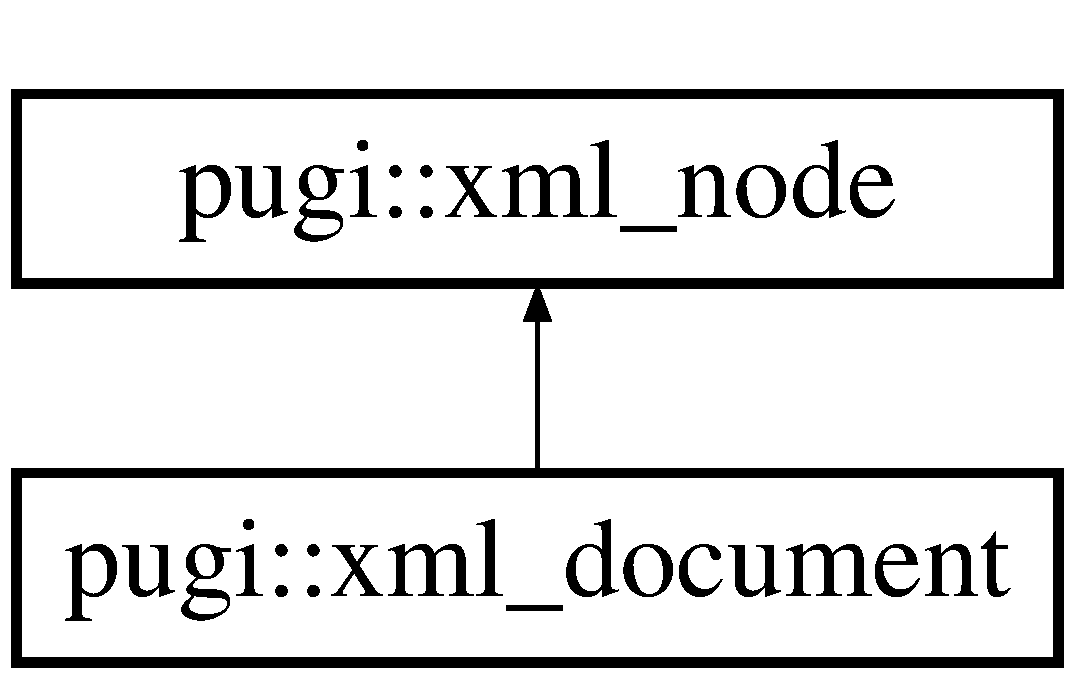
\includegraphics[height=2.000000cm]{classpugi_1_1xml__document}
\end{center}
\end{figure}
\subsection*{Public Member Functions}
\begin{DoxyCompactItemize}
\item 
\hyperlink{classpugi_1_1xml__document_afa82ca6827bda8504ce7dadbc443fa21}{xml\-\_\-document} ()
\item 
\hyperlink{classpugi_1_1xml__document_af37d8a79f7465ad48d65c2bd13461580}{$\sim$xml\-\_\-document} ()
\item 
void \hyperlink{classpugi_1_1xml__document_acf2b9daf1d12e12048796118b7a7685d}{reset} ()
\item 
void \hyperlink{classpugi_1_1xml__document_a4230de3de88f4fe481c4c3d5312aa5cf}{reset} (const \hyperlink{classpugi_1_1xml__document}{xml\-\_\-document} \&proto)
\item 
\hyperlink{structpugi_1_1xml__parse__result}{xml\-\_\-parse\-\_\-result} \hyperlink{classpugi_1_1xml__document_abb7db3882f94ac35b870510789a87778}{load} (std\-::basic\-\_\-istream$<$ char, std\-::char\-\_\-traits$<$ char $>$ $>$ \&stream, unsigned int options=\hyperlink{namespacepugi_ad7c927d1c1752330637c3318b0d7b366}{parse\-\_\-default}, \hyperlink{namespacepugi_a03f708f86abeff5fce6842ffd6a0951e}{xml\-\_\-encoding} encoding=\hyperlink{namespacepugi_a03f708f86abeff5fce6842ffd6a0951eae11b2ef666f03e77b7e764e38d22dc17}{encoding\-\_\-auto})
\item 
\hyperlink{structpugi_1_1xml__parse__result}{xml\-\_\-parse\-\_\-result} \hyperlink{classpugi_1_1xml__document_a36131b6f1a80a1248666f4e7fe352685}{load} (std\-::basic\-\_\-istream$<$ wchar\-\_\-t, std\-::char\-\_\-traits$<$ wchar\-\_\-t $>$ $>$ \&stream, unsigned int options=\hyperlink{namespacepugi_ad7c927d1c1752330637c3318b0d7b366}{parse\-\_\-default})
\item 
\hyperlink{structpugi_1_1xml__parse__result}{xml\-\_\-parse\-\_\-result} \hyperlink{classpugi_1_1xml__document_ae17a77772fa21a40f3d91d9c79e60d0b}{load} (const \hyperlink{namespacepugi_aef5a7a62cba0507542220ea15afe39df}{char\-\_\-t} $\ast$contents, unsigned int options=\hyperlink{namespacepugi_ad7c927d1c1752330637c3318b0d7b366}{parse\-\_\-default})
\item 
\hyperlink{structpugi_1_1xml__parse__result}{xml\-\_\-parse\-\_\-result} \hyperlink{classpugi_1_1xml__document_aad350209a4a91589fbd7e8cdaf79e010}{load\-\_\-file} (const char $\ast$\hyperlink{classpugi_1_1xml__node_ae5694be88058346ad8e6e418410d4979}{path}, unsigned int options=\hyperlink{namespacepugi_ad7c927d1c1752330637c3318b0d7b366}{parse\-\_\-default}, \hyperlink{namespacepugi_a03f708f86abeff5fce6842ffd6a0951e}{xml\-\_\-encoding} encoding=\hyperlink{namespacepugi_a03f708f86abeff5fce6842ffd6a0951eae11b2ef666f03e77b7e764e38d22dc17}{encoding\-\_\-auto})
\item 
\hyperlink{structpugi_1_1xml__parse__result}{xml\-\_\-parse\-\_\-result} \hyperlink{classpugi_1_1xml__document_ac5a29d9c9e754120a5e0c072b332a25a}{load\-\_\-file} (const wchar\-\_\-t $\ast$\hyperlink{classpugi_1_1xml__node_ae5694be88058346ad8e6e418410d4979}{path}, unsigned int options=\hyperlink{namespacepugi_ad7c927d1c1752330637c3318b0d7b366}{parse\-\_\-default}, \hyperlink{namespacepugi_a03f708f86abeff5fce6842ffd6a0951e}{xml\-\_\-encoding} encoding=\hyperlink{namespacepugi_a03f708f86abeff5fce6842ffd6a0951eae11b2ef666f03e77b7e764e38d22dc17}{encoding\-\_\-auto})
\item 
\hyperlink{structpugi_1_1xml__parse__result}{xml\-\_\-parse\-\_\-result} \hyperlink{classpugi_1_1xml__document_ab29840790e26b2166a395c63a2b2d9bd}{load\-\_\-buffer} (const void $\ast$contents, size\-\_\-t size, unsigned int options=\hyperlink{namespacepugi_ad7c927d1c1752330637c3318b0d7b366}{parse\-\_\-default}, \hyperlink{namespacepugi_a03f708f86abeff5fce6842ffd6a0951e}{xml\-\_\-encoding} encoding=\hyperlink{namespacepugi_a03f708f86abeff5fce6842ffd6a0951eae11b2ef666f03e77b7e764e38d22dc17}{encoding\-\_\-auto})
\item 
\hyperlink{structpugi_1_1xml__parse__result}{xml\-\_\-parse\-\_\-result} \hyperlink{classpugi_1_1xml__document_a3e20650182ccbdd175ca069dd5e08632}{load\-\_\-buffer\-\_\-inplace} (void $\ast$contents, size\-\_\-t size, unsigned int options=\hyperlink{namespacepugi_ad7c927d1c1752330637c3318b0d7b366}{parse\-\_\-default}, \hyperlink{namespacepugi_a03f708f86abeff5fce6842ffd6a0951e}{xml\-\_\-encoding} encoding=\hyperlink{namespacepugi_a03f708f86abeff5fce6842ffd6a0951eae11b2ef666f03e77b7e764e38d22dc17}{encoding\-\_\-auto})
\item 
\hyperlink{structpugi_1_1xml__parse__result}{xml\-\_\-parse\-\_\-result} \hyperlink{classpugi_1_1xml__document_a9da4bdcdc4ad914fb0f4680b02983502}{load\-\_\-buffer\-\_\-inplace\-\_\-own} (void $\ast$contents, size\-\_\-t size, unsigned int options=\hyperlink{namespacepugi_ad7c927d1c1752330637c3318b0d7b366}{parse\-\_\-default}, \hyperlink{namespacepugi_a03f708f86abeff5fce6842ffd6a0951e}{xml\-\_\-encoding} encoding=\hyperlink{namespacepugi_a03f708f86abeff5fce6842ffd6a0951eae11b2ef666f03e77b7e764e38d22dc17}{encoding\-\_\-auto})
\item 
void \hyperlink{classpugi_1_1xml__document_ae69983f0991300cc9afc8891ff9ca4ac}{save} (\hyperlink{classpugi_1_1xml__writer}{xml\-\_\-writer} \&writer, const \hyperlink{namespacepugi_aef5a7a62cba0507542220ea15afe39df}{char\-\_\-t} $\ast$indent=\hyperlink{pugixml_8hpp_ad5475bca2e336810ae5906349e644d0b}{P\-U\-G\-I\-X\-M\-L\-\_\-\-T\-E\-X\-T}(\char`\"{}\textbackslash{}t\char`\"{}), unsigned int flags=\hyperlink{namespacepugi_a325f48a35abbaeacdfd8b7fc9ed1713c}{format\-\_\-default}, \hyperlink{namespacepugi_a03f708f86abeff5fce6842ffd6a0951e}{xml\-\_\-encoding} encoding=\hyperlink{namespacepugi_a03f708f86abeff5fce6842ffd6a0951eae11b2ef666f03e77b7e764e38d22dc17}{encoding\-\_\-auto}) const 
\item 
void \hyperlink{classpugi_1_1xml__document_a471d7354af62da143f10943057c99ffa}{save} (std\-::basic\-\_\-ostream$<$ char, std\-::char\-\_\-traits$<$ char $>$ $>$ \&stream, const \hyperlink{namespacepugi_aef5a7a62cba0507542220ea15afe39df}{char\-\_\-t} $\ast$indent=\hyperlink{pugixml_8hpp_ad5475bca2e336810ae5906349e644d0b}{P\-U\-G\-I\-X\-M\-L\-\_\-\-T\-E\-X\-T}(\char`\"{}\textbackslash{}t\char`\"{}), unsigned int flags=\hyperlink{namespacepugi_a325f48a35abbaeacdfd8b7fc9ed1713c}{format\-\_\-default}, \hyperlink{namespacepugi_a03f708f86abeff5fce6842ffd6a0951e}{xml\-\_\-encoding} encoding=\hyperlink{namespacepugi_a03f708f86abeff5fce6842ffd6a0951eae11b2ef666f03e77b7e764e38d22dc17}{encoding\-\_\-auto}) const 
\item 
void \hyperlink{classpugi_1_1xml__document_ae0b377bda28c7fbac4ba50b4e3f9d211}{save} (std\-::basic\-\_\-ostream$<$ wchar\-\_\-t, std\-::char\-\_\-traits$<$ wchar\-\_\-t $>$ $>$ \&stream, const \hyperlink{namespacepugi_aef5a7a62cba0507542220ea15afe39df}{char\-\_\-t} $\ast$indent=\hyperlink{pugixml_8hpp_ad5475bca2e336810ae5906349e644d0b}{P\-U\-G\-I\-X\-M\-L\-\_\-\-T\-E\-X\-T}(\char`\"{}\textbackslash{}t\char`\"{}), unsigned int flags=\hyperlink{namespacepugi_a325f48a35abbaeacdfd8b7fc9ed1713c}{format\-\_\-default}) const 
\item 
bool \hyperlink{classpugi_1_1xml__document_ac67294573cbaa41d3e6210480a9f7f99}{save\-\_\-file} (const char $\ast$\hyperlink{classpugi_1_1xml__node_ae5694be88058346ad8e6e418410d4979}{path}, const \hyperlink{namespacepugi_aef5a7a62cba0507542220ea15afe39df}{char\-\_\-t} $\ast$indent=\hyperlink{pugixml_8hpp_ad5475bca2e336810ae5906349e644d0b}{P\-U\-G\-I\-X\-M\-L\-\_\-\-T\-E\-X\-T}(\char`\"{}\textbackslash{}t\char`\"{}), unsigned int flags=\hyperlink{namespacepugi_a325f48a35abbaeacdfd8b7fc9ed1713c}{format\-\_\-default}, \hyperlink{namespacepugi_a03f708f86abeff5fce6842ffd6a0951e}{xml\-\_\-encoding} encoding=\hyperlink{namespacepugi_a03f708f86abeff5fce6842ffd6a0951eae11b2ef666f03e77b7e764e38d22dc17}{encoding\-\_\-auto}) const 
\item 
bool \hyperlink{classpugi_1_1xml__document_a47e18cd3438eabd64fa2f82d56b08aef}{save\-\_\-file} (const wchar\-\_\-t $\ast$\hyperlink{classpugi_1_1xml__node_ae5694be88058346ad8e6e418410d4979}{path}, const \hyperlink{namespacepugi_aef5a7a62cba0507542220ea15afe39df}{char\-\_\-t} $\ast$indent=\hyperlink{pugixml_8hpp_ad5475bca2e336810ae5906349e644d0b}{P\-U\-G\-I\-X\-M\-L\-\_\-\-T\-E\-X\-T}(\char`\"{}\textbackslash{}t\char`\"{}), unsigned int flags=\hyperlink{namespacepugi_a325f48a35abbaeacdfd8b7fc9ed1713c}{format\-\_\-default}, \hyperlink{namespacepugi_a03f708f86abeff5fce6842ffd6a0951e}{xml\-\_\-encoding} encoding=\hyperlink{namespacepugi_a03f708f86abeff5fce6842ffd6a0951eae11b2ef666f03e77b7e764e38d22dc17}{encoding\-\_\-auto}) const 
\item 
\hyperlink{classpugi_1_1xml__node}{xml\-\_\-node} \hyperlink{classpugi_1_1xml__document_aa3b17a8891e2c89996ab4c7a2a6759ad}{document\-\_\-element} () const 
\end{DoxyCompactItemize}
\subsection*{Additional Inherited Members}


\subsection{Constructor \& Destructor Documentation}
\hypertarget{classpugi_1_1xml__document_afa82ca6827bda8504ce7dadbc443fa21}{\index{pugi\-::xml\-\_\-document@{pugi\-::xml\-\_\-document}!xml\-\_\-document@{xml\-\_\-document}}
\index{xml\-\_\-document@{xml\-\_\-document}!pugi::xml_document@{pugi\-::xml\-\_\-document}}
\subsubsection[{xml\-\_\-document}]{\setlength{\rightskip}{0pt plus 5cm}{\bf P\-U\-G\-I\-\_\-\-\_\-\-F\-N} pugi\-::xml\-\_\-document\-::xml\-\_\-document (
\begin{DoxyParamCaption}
{}
\end{DoxyParamCaption}
)}}\label{classpugi_1_1xml__document_afa82ca6827bda8504ce7dadbc443fa21}

\begin{DoxyCode}
5102                                        : \_buffer(0)
5103     \{
5104         create();
5105     \}
\end{DoxyCode}
\hypertarget{classpugi_1_1xml__document_af37d8a79f7465ad48d65c2bd13461580}{\index{pugi\-::xml\-\_\-document@{pugi\-::xml\-\_\-document}!$\sim$xml\-\_\-document@{$\sim$xml\-\_\-document}}
\index{$\sim$xml\-\_\-document@{$\sim$xml\-\_\-document}!pugi::xml_document@{pugi\-::xml\-\_\-document}}
\subsubsection[{$\sim$xml\-\_\-document}]{\setlength{\rightskip}{0pt plus 5cm}{\bf P\-U\-G\-I\-\_\-\-\_\-\-F\-N} pugi\-::xml\-\_\-document\-::$\sim$xml\-\_\-document (
\begin{DoxyParamCaption}
{}
\end{DoxyParamCaption}
)}}\label{classpugi_1_1xml__document_af37d8a79f7465ad48d65c2bd13461580}

\begin{DoxyCode}
5108     \{
5109         destroy();
5110     \}
\end{DoxyCode}


\subsection{Member Function Documentation}
\hypertarget{classpugi_1_1xml__document_aa3b17a8891e2c89996ab4c7a2a6759ad}{\index{pugi\-::xml\-\_\-document@{pugi\-::xml\-\_\-document}!document\-\_\-element@{document\-\_\-element}}
\index{document\-\_\-element@{document\-\_\-element}!pugi::xml_document@{pugi\-::xml\-\_\-document}}
\subsubsection[{document\-\_\-element}]{\setlength{\rightskip}{0pt plus 5cm}{\bf P\-U\-G\-I\-\_\-\-\_\-\-F\-N} {\bf xml\-\_\-node} pugi\-::xml\-\_\-document\-::document\-\_\-element (
\begin{DoxyParamCaption}
{}
\end{DoxyParamCaption}
) const}}\label{classpugi_1_1xml__document_aa3b17a8891e2c89996ab4c7a2a6759ad}

\begin{DoxyCode}
5328     \{
5329         \textcolor{keywordflow}{for} (xml\_node\_struct* i = \hyperlink{classpugi_1_1xml__node_a45a5b342de1e37a60565f7693f03cc08}{\_root}->\hyperlink{structpugi_1_1xml__node__struct_af72c49a0f81928ef664d9d2f0260f23d}{first\_child}; i; i = i->
      \hyperlink{structpugi_1_1xml__node__struct_acf0867e3a77871e37132046d97398a6d}{next\_sibling})
5330             \textcolor{keywordflow}{if} ((i->header & impl::xml\_memory\_page\_type\_mask) + 1 == 
      \hyperlink{namespacepugi_a137e94a038e4ab0ada6477cf7f6153a9a6d223e3a0d8ce8e4ee6f4a2697b8bcd1}{node\_element})
5331                 \textcolor{keywordflow}{return} \hyperlink{classpugi_1_1xml__node_a36ec0eb8b399d71f6b55be0e181c69f9}{xml\_node}(i);
5332 
5333         \textcolor{keywordflow}{return} \hyperlink{classpugi_1_1xml__node_a36ec0eb8b399d71f6b55be0e181c69f9}{xml\_node}();
5334     \}
\end{DoxyCode}
\hypertarget{classpugi_1_1xml__document_abb7db3882f94ac35b870510789a87778}{\index{pugi\-::xml\-\_\-document@{pugi\-::xml\-\_\-document}!load@{load}}
\index{load@{load}!pugi::xml_document@{pugi\-::xml\-\_\-document}}
\subsubsection[{load}]{\setlength{\rightskip}{0pt plus 5cm}{\bf P\-U\-G\-I\-\_\-\-\_\-\-F\-N} {\bf xml\-\_\-parse\-\_\-result} pugi\-::xml\-\_\-document\-::load (
\begin{DoxyParamCaption}
\item[{std\-::basic\-\_\-istream$<$ char, std\-::char\-\_\-traits$<$ char $>$ $>$ \&}]{stream, }
\item[{unsigned int}]{options = {\ttfamily {\bf parse\-\_\-default}}, }
\item[{{\bf xml\-\_\-encoding}}]{encoding = {\ttfamily {\bf encoding\-\_\-auto}}}
\end{DoxyParamCaption}
)}}\label{classpugi_1_1xml__document_abb7db3882f94ac35b870510789a87778}

\begin{DoxyCode}
5183     \{
5184         \hyperlink{classpugi_1_1xml__document_acf2b9daf1d12e12048796118b7a7685d}{reset}();
5185 
5186         \textcolor{keywordflow}{return} \hyperlink{pugixml_8cpp_a3515ac8101e357707f45d7438d568682}{impl::load\_stream\_impl}(*\textcolor{keyword}{this}, stream, options, encoding);
5187     \}
\end{DoxyCode}
\hypertarget{classpugi_1_1xml__document_a36131b6f1a80a1248666f4e7fe352685}{\index{pugi\-::xml\-\_\-document@{pugi\-::xml\-\_\-document}!load@{load}}
\index{load@{load}!pugi::xml_document@{pugi\-::xml\-\_\-document}}
\subsubsection[{load}]{\setlength{\rightskip}{0pt plus 5cm}{\bf P\-U\-G\-I\-\_\-\-\_\-\-F\-N} {\bf xml\-\_\-parse\-\_\-result} pugi\-::xml\-\_\-document\-::load (
\begin{DoxyParamCaption}
\item[{std\-::basic\-\_\-istream$<$ wchar\-\_\-t, std\-::char\-\_\-traits$<$ wchar\-\_\-t $>$ $>$ \&}]{stream, }
\item[{unsigned int}]{options = {\ttfamily {\bf parse\-\_\-default}}}
\end{DoxyParamCaption}
)}}\label{classpugi_1_1xml__document_a36131b6f1a80a1248666f4e7fe352685}

\begin{DoxyCode}
5190     \{
5191         \hyperlink{classpugi_1_1xml__document_acf2b9daf1d12e12048796118b7a7685d}{reset}();
5192 
5193         \textcolor{keywordflow}{return} \hyperlink{pugixml_8cpp_a3515ac8101e357707f45d7438d568682}{impl::load\_stream\_impl}(*\textcolor{keyword}{this}, stream, options, 
      \hyperlink{namespacepugi_a03f708f86abeff5fce6842ffd6a0951eae670d39438f31fe41f1a596739e5c00e}{encoding\_wchar});
5194     \}
\end{DoxyCode}
\hypertarget{classpugi_1_1xml__document_ae17a77772fa21a40f3d91d9c79e60d0b}{\index{pugi\-::xml\-\_\-document@{pugi\-::xml\-\_\-document}!load@{load}}
\index{load@{load}!pugi::xml_document@{pugi\-::xml\-\_\-document}}
\subsubsection[{load}]{\setlength{\rightskip}{0pt plus 5cm}{\bf P\-U\-G\-I\-\_\-\-\_\-\-F\-N} {\bf xml\-\_\-parse\-\_\-result} pugi\-::xml\-\_\-document\-::load (
\begin{DoxyParamCaption}
\item[{const {\bf char\-\_\-t} $\ast$}]{contents, }
\item[{unsigned int}]{options = {\ttfamily {\bf parse\-\_\-default}}}
\end{DoxyParamCaption}
)}}\label{classpugi_1_1xml__document_ae17a77772fa21a40f3d91d9c79e60d0b}

\begin{DoxyCode}
5198     \{
5199         \textcolor{comment}{// Force native encoding (skip autodetection)}
5200 \textcolor{preprocessor}{    #ifdef PUGIXML\_WCHAR\_MODE}
5201 \textcolor{preprocessor}{}        \hyperlink{namespacepugi_a03f708f86abeff5fce6842ffd6a0951e}{xml\_encoding} encoding = \hyperlink{namespacepugi_a03f708f86abeff5fce6842ffd6a0951eae670d39438f31fe41f1a596739e5c00e}{encoding\_wchar};
5202 \textcolor{preprocessor}{    #else}
5203 \textcolor{preprocessor}{}        \hyperlink{namespacepugi_a03f708f86abeff5fce6842ffd6a0951e}{xml\_encoding} encoding = \hyperlink{namespacepugi_a03f708f86abeff5fce6842ffd6a0951ea96c73bf345f635f0fbee5f6646fb095e}{encoding\_utf8};
5204 \textcolor{preprocessor}{    #endif}
5205 \textcolor{preprocessor}{}
5206         \textcolor{keywordflow}{return} \hyperlink{classpugi_1_1xml__document_ab29840790e26b2166a395c63a2b2d9bd}{load\_buffer}(contents, \hyperlink{pugixml_8cpp_aab9e1f034d085b663d146fcceabb1c48}{impl::strlength}(contents) * \textcolor{keyword}{sizeof}(
      \hyperlink{namespacepugi_aef5a7a62cba0507542220ea15afe39df}{char\_t}), options, encoding);
5207     \}
\end{DoxyCode}
\hypertarget{classpugi_1_1xml__document_ab29840790e26b2166a395c63a2b2d9bd}{\index{pugi\-::xml\-\_\-document@{pugi\-::xml\-\_\-document}!load\-\_\-buffer@{load\-\_\-buffer}}
\index{load\-\_\-buffer@{load\-\_\-buffer}!pugi::xml_document@{pugi\-::xml\-\_\-document}}
\subsubsection[{load\-\_\-buffer}]{\setlength{\rightskip}{0pt plus 5cm}{\bf P\-U\-G\-I\-\_\-\-\_\-\-F\-N} {\bf xml\-\_\-parse\-\_\-result} pugi\-::xml\-\_\-document\-::load\-\_\-buffer (
\begin{DoxyParamCaption}
\item[{const void $\ast$}]{contents, }
\item[{size\-\_\-t}]{size, }
\item[{unsigned int}]{options = {\ttfamily {\bf parse\-\_\-default}}, }
\item[{{\bf xml\-\_\-encoding}}]{encoding = {\ttfamily {\bf encoding\-\_\-auto}}}
\end{DoxyParamCaption}
)}}\label{classpugi_1_1xml__document_ab29840790e26b2166a395c63a2b2d9bd}

\begin{DoxyCode}
5259     \{
5260         \textcolor{keywordflow}{return} load\_buffer\_impl(const\_cast<void*>(contents), size, options, encoding, \textcolor{keyword}{false}, \textcolor{keyword}{false});
5261     \}
\end{DoxyCode}
\hypertarget{classpugi_1_1xml__document_a3e20650182ccbdd175ca069dd5e08632}{\index{pugi\-::xml\-\_\-document@{pugi\-::xml\-\_\-document}!load\-\_\-buffer\-\_\-inplace@{load\-\_\-buffer\-\_\-inplace}}
\index{load\-\_\-buffer\-\_\-inplace@{load\-\_\-buffer\-\_\-inplace}!pugi::xml_document@{pugi\-::xml\-\_\-document}}
\subsubsection[{load\-\_\-buffer\-\_\-inplace}]{\setlength{\rightskip}{0pt plus 5cm}{\bf P\-U\-G\-I\-\_\-\-\_\-\-F\-N} {\bf xml\-\_\-parse\-\_\-result} pugi\-::xml\-\_\-document\-::load\-\_\-buffer\-\_\-inplace (
\begin{DoxyParamCaption}
\item[{void $\ast$}]{contents, }
\item[{size\-\_\-t}]{size, }
\item[{unsigned int}]{options = {\ttfamily {\bf parse\-\_\-default}}, }
\item[{{\bf xml\-\_\-encoding}}]{encoding = {\ttfamily {\bf encoding\-\_\-auto}}}
\end{DoxyParamCaption}
)}}\label{classpugi_1_1xml__document_a3e20650182ccbdd175ca069dd5e08632}

\begin{DoxyCode}
5264     \{
5265         \textcolor{keywordflow}{return} load\_buffer\_impl(contents, size, options, encoding, \textcolor{keyword}{true}, \textcolor{keyword}{false});
5266     \}
\end{DoxyCode}
\hypertarget{classpugi_1_1xml__document_a9da4bdcdc4ad914fb0f4680b02983502}{\index{pugi\-::xml\-\_\-document@{pugi\-::xml\-\_\-document}!load\-\_\-buffer\-\_\-inplace\-\_\-own@{load\-\_\-buffer\-\_\-inplace\-\_\-own}}
\index{load\-\_\-buffer\-\_\-inplace\-\_\-own@{load\-\_\-buffer\-\_\-inplace\-\_\-own}!pugi::xml_document@{pugi\-::xml\-\_\-document}}
\subsubsection[{load\-\_\-buffer\-\_\-inplace\-\_\-own}]{\setlength{\rightskip}{0pt plus 5cm}{\bf P\-U\-G\-I\-\_\-\-\_\-\-F\-N} {\bf xml\-\_\-parse\-\_\-result} pugi\-::xml\-\_\-document\-::load\-\_\-buffer\-\_\-inplace\-\_\-own (
\begin{DoxyParamCaption}
\item[{void $\ast$}]{contents, }
\item[{size\-\_\-t}]{size, }
\item[{unsigned int}]{options = {\ttfamily {\bf parse\-\_\-default}}, }
\item[{{\bf xml\-\_\-encoding}}]{encoding = {\ttfamily {\bf encoding\-\_\-auto}}}
\end{DoxyParamCaption}
)}}\label{classpugi_1_1xml__document_a9da4bdcdc4ad914fb0f4680b02983502}

\begin{DoxyCode}
5269     \{
5270         \textcolor{keywordflow}{return} load\_buffer\_impl(contents, size, options, encoding, \textcolor{keyword}{true}, \textcolor{keyword}{true});
5271     \}
\end{DoxyCode}
\hypertarget{classpugi_1_1xml__document_aad350209a4a91589fbd7e8cdaf79e010}{\index{pugi\-::xml\-\_\-document@{pugi\-::xml\-\_\-document}!load\-\_\-file@{load\-\_\-file}}
\index{load\-\_\-file@{load\-\_\-file}!pugi::xml_document@{pugi\-::xml\-\_\-document}}
\subsubsection[{load\-\_\-file}]{\setlength{\rightskip}{0pt plus 5cm}{\bf P\-U\-G\-I\-\_\-\-\_\-\-F\-N} {\bf xml\-\_\-parse\-\_\-result} pugi\-::xml\-\_\-document\-::load\-\_\-file (
\begin{DoxyParamCaption}
\item[{const char $\ast$}]{path, }
\item[{unsigned int}]{options = {\ttfamily {\bf parse\-\_\-default}}, }
\item[{{\bf xml\-\_\-encoding}}]{encoding = {\ttfamily {\bf encoding\-\_\-auto}}}
\end{DoxyParamCaption}
)}}\label{classpugi_1_1xml__document_aad350209a4a91589fbd7e8cdaf79e010}

\begin{DoxyCode}
5210     \{
5211         \hyperlink{classpugi_1_1xml__document_acf2b9daf1d12e12048796118b7a7685d}{reset}();
5212 
5213         FILE* file = fopen(path\_, \textcolor{stringliteral}{"rb"});
5214 
5215         \textcolor{keywordflow}{return} \hyperlink{pugixml_8cpp_a79f0e2f9483c87a85ec4873a20caaa12}{impl::load\_file\_impl}(*\textcolor{keyword}{this}, file, options, encoding);
5216     \}
\end{DoxyCode}
\hypertarget{classpugi_1_1xml__document_ac5a29d9c9e754120a5e0c072b332a25a}{\index{pugi\-::xml\-\_\-document@{pugi\-::xml\-\_\-document}!load\-\_\-file@{load\-\_\-file}}
\index{load\-\_\-file@{load\-\_\-file}!pugi::xml_document@{pugi\-::xml\-\_\-document}}
\subsubsection[{load\-\_\-file}]{\setlength{\rightskip}{0pt plus 5cm}{\bf P\-U\-G\-I\-\_\-\-\_\-\-F\-N} {\bf xml\-\_\-parse\-\_\-result} pugi\-::xml\-\_\-document\-::load\-\_\-file (
\begin{DoxyParamCaption}
\item[{const wchar\-\_\-t $\ast$}]{path, }
\item[{unsigned int}]{options = {\ttfamily {\bf parse\-\_\-default}}, }
\item[{{\bf xml\-\_\-encoding}}]{encoding = {\ttfamily {\bf encoding\-\_\-auto}}}
\end{DoxyParamCaption}
)}}\label{classpugi_1_1xml__document_ac5a29d9c9e754120a5e0c072b332a25a}

\begin{DoxyCode}
5219     \{
5220         \hyperlink{classpugi_1_1xml__document_acf2b9daf1d12e12048796118b7a7685d}{reset}();
5221 
5222         FILE* file = \hyperlink{pugixml_8cpp_a6a347080c51ac7c992a32cde66a43801}{impl::open\_file\_wide}(path\_, L\textcolor{stringliteral}{"rb"});
5223 
5224         \textcolor{keywordflow}{return} \hyperlink{pugixml_8cpp_a79f0e2f9483c87a85ec4873a20caaa12}{impl::load\_file\_impl}(*\textcolor{keyword}{this}, file, options, encoding);
5225     \}
\end{DoxyCode}
\hypertarget{classpugi_1_1xml__document_acf2b9daf1d12e12048796118b7a7685d}{\index{pugi\-::xml\-\_\-document@{pugi\-::xml\-\_\-document}!reset@{reset}}
\index{reset@{reset}!pugi::xml_document@{pugi\-::xml\-\_\-document}}
\subsubsection[{reset}]{\setlength{\rightskip}{0pt plus 5cm}{\bf P\-U\-G\-I\-\_\-\-\_\-\-F\-N} void pugi\-::xml\-\_\-document\-::reset (
\begin{DoxyParamCaption}
{}
\end{DoxyParamCaption}
)}}\label{classpugi_1_1xml__document_acf2b9daf1d12e12048796118b7a7685d}

\begin{DoxyCode}
5113     \{
5114         destroy();
5115         create();
5116     \}
\end{DoxyCode}
\hypertarget{classpugi_1_1xml__document_a4230de3de88f4fe481c4c3d5312aa5cf}{\index{pugi\-::xml\-\_\-document@{pugi\-::xml\-\_\-document}!reset@{reset}}
\index{reset@{reset}!pugi::xml_document@{pugi\-::xml\-\_\-document}}
\subsubsection[{reset}]{\setlength{\rightskip}{0pt plus 5cm}{\bf P\-U\-G\-I\-\_\-\-\_\-\-F\-N} void pugi\-::xml\-\_\-document\-::reset (
\begin{DoxyParamCaption}
\item[{const {\bf xml\-\_\-document} \&}]{proto}
\end{DoxyParamCaption}
)}}\label{classpugi_1_1xml__document_a4230de3de88f4fe481c4c3d5312aa5cf}

\begin{DoxyCode}
5119     \{
5120         \hyperlink{classpugi_1_1xml__document_acf2b9daf1d12e12048796118b7a7685d}{reset}();
5121 
5122         \textcolor{keywordflow}{for} (\hyperlink{classpugi_1_1xml__node_a36ec0eb8b399d71f6b55be0e181c69f9}{xml\_node} cur = proto.first\_child(); cur; cur = cur.next\_sibling())
5123             \hyperlink{classpugi_1_1xml__node_a4c151e6665c6bfa614fe80d177fd5396}{append\_copy}(cur);
5124     \}
\end{DoxyCode}
\hypertarget{classpugi_1_1xml__document_ae69983f0991300cc9afc8891ff9ca4ac}{\index{pugi\-::xml\-\_\-document@{pugi\-::xml\-\_\-document}!save@{save}}
\index{save@{save}!pugi::xml_document@{pugi\-::xml\-\_\-document}}
\subsubsection[{save}]{\setlength{\rightskip}{0pt plus 5cm}{\bf P\-U\-G\-I\-\_\-\-\_\-\-F\-N} void pugi\-::xml\-\_\-document\-::save (
\begin{DoxyParamCaption}
\item[{{\bf xml\-\_\-writer} \&}]{writer, }
\item[{const {\bf char\-\_\-t} $\ast$}]{indent = {\ttfamily {\bf P\-U\-G\-I\-X\-M\-L\-\_\-\-T\-E\-X\-T}(\char`\"{}\textbackslash{}t\char`\"{})}, }
\item[{unsigned int}]{flags = {\ttfamily {\bf format\-\_\-default}}, }
\item[{{\bf xml\-\_\-encoding}}]{encoding = {\ttfamily {\bf encoding\-\_\-auto}}}
\end{DoxyParamCaption}
) const}}\label{classpugi_1_1xml__document_ae69983f0991300cc9afc8891ff9ca4ac}

\begin{DoxyCode}
5274     \{
5275         impl::xml\_buffered\_writer buffered\_writer(writer, encoding);
5276 
5277         \textcolor{keywordflow}{if} ((flags & \hyperlink{namespacepugi_ab863bcafd203aeaa98953df3a998243f}{format\_write\_bom}) && encoding != 
      \hyperlink{namespacepugi_a03f708f86abeff5fce6842ffd6a0951ea9f1a8dbbf996bcd297ce0922b7eec40d}{encoding\_latin1})
5278         \{
5279             \textcolor{comment}{// BOM always represents the codepoint U+FEFF, so just write it in native encoding}
5280 \textcolor{preprocessor}{        #ifdef PUGIXML\_WCHAR\_MODE}
5281 \textcolor{preprocessor}{}            \textcolor{keywordtype}{unsigned} \textcolor{keywordtype}{int} bom = 0xfeff;
5282             buffered\_writer.write(static\_cast<wchar\_t>(bom));
5283 \textcolor{preprocessor}{        #else}
5284 \textcolor{preprocessor}{}            buffered\_writer.write(\textcolor{stringliteral}{'\(\backslash\)xef'}, \textcolor{stringliteral}{'\(\backslash\)xbb'}, \textcolor{stringliteral}{'\(\backslash\)xbf'});
5285 \textcolor{preprocessor}{        #endif}
5286 \textcolor{preprocessor}{}        \}
5287 
5288         \textcolor{keywordflow}{if} (!(flags & \hyperlink{namespacepugi_a0ec33e4db09260718f7003ed091f5a1b}{format\_no\_declaration}) && !
      \hyperlink{pugixml_8cpp_a51b27832195cf2345f65119f07056743}{impl::has\_declaration}(*\textcolor{keyword}{this}))
5289         \{
5290             buffered\_writer.write(\hyperlink{pugixml_8hpp_ad5475bca2e336810ae5906349e644d0b}{PUGIXML\_TEXT}(\textcolor{stringliteral}{"<?xml version=\(\backslash\)"1.0\(\backslash\)""}));
5291             \textcolor{keywordflow}{if} (encoding == \hyperlink{namespacepugi_a03f708f86abeff5fce6842ffd6a0951ea9f1a8dbbf996bcd297ce0922b7eec40d}{encoding\_latin1}) buffered\_writer.write(
      \hyperlink{pugixml_8hpp_ad5475bca2e336810ae5906349e644d0b}{PUGIXML\_TEXT}(\textcolor{stringliteral}{" encoding=\(\backslash\)"ISO-8859-1\(\backslash\)""}));
5292             buffered\_writer.write(\textcolor{charliteral}{'?'}, \textcolor{charliteral}{'>'});
5293             \textcolor{keywordflow}{if} (!(flags & \hyperlink{namespacepugi_a2dd811716b1c0a6a2431ceca43bc649e}{format\_raw})) buffered\_writer.write(\textcolor{charliteral}{'\(\backslash\)n'});
5294         \}
5295 
5296         \hyperlink{pugixml_8cpp_a7f5dd565c9321db184119a5f337333e7}{impl::node\_output}(buffered\_writer, *\textcolor{keyword}{this}, indent, flags, 0);
5297     \}
\end{DoxyCode}
\hypertarget{classpugi_1_1xml__document_a471d7354af62da143f10943057c99ffa}{\index{pugi\-::xml\-\_\-document@{pugi\-::xml\-\_\-document}!save@{save}}
\index{save@{save}!pugi::xml_document@{pugi\-::xml\-\_\-document}}
\subsubsection[{save}]{\setlength{\rightskip}{0pt plus 5cm}{\bf P\-U\-G\-I\-\_\-\-\_\-\-F\-N} void pugi\-::xml\-\_\-document\-::save (
\begin{DoxyParamCaption}
\item[{std\-::basic\-\_\-ostream$<$ char, std\-::char\-\_\-traits$<$ char $>$ $>$ \&}]{stream, }
\item[{const {\bf char\-\_\-t} $\ast$}]{indent = {\ttfamily {\bf P\-U\-G\-I\-X\-M\-L\-\_\-\-T\-E\-X\-T}(\char`\"{}\textbackslash{}t\char`\"{})}, }
\item[{unsigned int}]{flags = {\ttfamily {\bf format\-\_\-default}}, }
\item[{{\bf xml\-\_\-encoding}}]{encoding = {\ttfamily {\bf encoding\-\_\-auto}}}
\end{DoxyParamCaption}
) const}}\label{classpugi_1_1xml__document_a471d7354af62da143f10943057c99ffa}

\begin{DoxyCode}
5301     \{
5302         xml\_writer\_stream writer(stream);
5303 
5304         \hyperlink{classpugi_1_1xml__document_ae69983f0991300cc9afc8891ff9ca4ac}{save}(writer, indent, flags, encoding);
5305     \}
\end{DoxyCode}
\hypertarget{classpugi_1_1xml__document_ae0b377bda28c7fbac4ba50b4e3f9d211}{\index{pugi\-::xml\-\_\-document@{pugi\-::xml\-\_\-document}!save@{save}}
\index{save@{save}!pugi::xml_document@{pugi\-::xml\-\_\-document}}
\subsubsection[{save}]{\setlength{\rightskip}{0pt plus 5cm}{\bf P\-U\-G\-I\-\_\-\-\_\-\-F\-N} void pugi\-::xml\-\_\-document\-::save (
\begin{DoxyParamCaption}
\item[{std\-::basic\-\_\-ostream$<$ wchar\-\_\-t, std\-::char\-\_\-traits$<$ wchar\-\_\-t $>$ $>$ \&}]{stream, }
\item[{const {\bf char\-\_\-t} $\ast$}]{indent = {\ttfamily {\bf P\-U\-G\-I\-X\-M\-L\-\_\-\-T\-E\-X\-T}(\char`\"{}\textbackslash{}t\char`\"{})}, }
\item[{unsigned int}]{flags = {\ttfamily {\bf format\-\_\-default}}}
\end{DoxyParamCaption}
) const}}\label{classpugi_1_1xml__document_ae0b377bda28c7fbac4ba50b4e3f9d211}

\begin{DoxyCode}
5308     \{
5309         xml\_writer\_stream writer(stream);
5310 
5311         \hyperlink{classpugi_1_1xml__document_ae69983f0991300cc9afc8891ff9ca4ac}{save}(writer, indent, flags, \hyperlink{namespacepugi_a03f708f86abeff5fce6842ffd6a0951eae670d39438f31fe41f1a596739e5c00e}{encoding\_wchar});
5312     \}
\end{DoxyCode}
\hypertarget{classpugi_1_1xml__document_ac67294573cbaa41d3e6210480a9f7f99}{\index{pugi\-::xml\-\_\-document@{pugi\-::xml\-\_\-document}!save\-\_\-file@{save\-\_\-file}}
\index{save\-\_\-file@{save\-\_\-file}!pugi::xml_document@{pugi\-::xml\-\_\-document}}
\subsubsection[{save\-\_\-file}]{\setlength{\rightskip}{0pt plus 5cm}{\bf P\-U\-G\-I\-\_\-\-\_\-\-F\-N} bool pugi\-::xml\-\_\-document\-::save\-\_\-file (
\begin{DoxyParamCaption}
\item[{const char $\ast$}]{path, }
\item[{const {\bf char\-\_\-t} $\ast$}]{indent = {\ttfamily {\bf P\-U\-G\-I\-X\-M\-L\-\_\-\-T\-E\-X\-T}(\char`\"{}\textbackslash{}t\char`\"{})}, }
\item[{unsigned int}]{flags = {\ttfamily {\bf format\-\_\-default}}, }
\item[{{\bf xml\-\_\-encoding}}]{encoding = {\ttfamily {\bf encoding\-\_\-auto}}}
\end{DoxyParamCaption}
) const}}\label{classpugi_1_1xml__document_ac67294573cbaa41d3e6210480a9f7f99}

\begin{DoxyCode}
5316     \{
5317         FILE* file = fopen(path\_, (flags & \hyperlink{namespacepugi_ab0aae01dc0b870a2673c32ca6623ae09}{format\_save\_file\_text}) ? \textcolor{stringliteral}{"w"} : \textcolor{stringliteral}{"wb"});
5318         \textcolor{keywordflow}{return} \hyperlink{pugixml_8cpp_abde253604bc33c829133fdbc5d2b4dba}{impl::save\_file\_impl}(*\textcolor{keyword}{this}, file, indent, flags, encoding);
5319     \}
\end{DoxyCode}
\hypertarget{classpugi_1_1xml__document_a47e18cd3438eabd64fa2f82d56b08aef}{\index{pugi\-::xml\-\_\-document@{pugi\-::xml\-\_\-document}!save\-\_\-file@{save\-\_\-file}}
\index{save\-\_\-file@{save\-\_\-file}!pugi::xml_document@{pugi\-::xml\-\_\-document}}
\subsubsection[{save\-\_\-file}]{\setlength{\rightskip}{0pt plus 5cm}{\bf P\-U\-G\-I\-\_\-\-\_\-\-F\-N} bool pugi\-::xml\-\_\-document\-::save\-\_\-file (
\begin{DoxyParamCaption}
\item[{const wchar\-\_\-t $\ast$}]{path, }
\item[{const {\bf char\-\_\-t} $\ast$}]{indent = {\ttfamily {\bf P\-U\-G\-I\-X\-M\-L\-\_\-\-T\-E\-X\-T}(\char`\"{}\textbackslash{}t\char`\"{})}, }
\item[{unsigned int}]{flags = {\ttfamily {\bf format\-\_\-default}}, }
\item[{{\bf xml\-\_\-encoding}}]{encoding = {\ttfamily {\bf encoding\-\_\-auto}}}
\end{DoxyParamCaption}
) const}}\label{classpugi_1_1xml__document_a47e18cd3438eabd64fa2f82d56b08aef}

\begin{DoxyCode}
5322     \{
5323         FILE* file = \hyperlink{pugixml_8cpp_a6a347080c51ac7c992a32cde66a43801}{impl::open\_file\_wide}(path\_, (flags & 
      \hyperlink{namespacepugi_ab0aae01dc0b870a2673c32ca6623ae09}{format\_save\_file\_text}) ? L\textcolor{stringliteral}{"w"} : L\textcolor{stringliteral}{"wb"});
5324         \textcolor{keywordflow}{return} \hyperlink{pugixml_8cpp_abde253604bc33c829133fdbc5d2b4dba}{impl::save\_file\_impl}(*\textcolor{keyword}{this}, file, indent, flags, encoding);
5325     \}
\end{DoxyCode}


The documentation for this class was generated from the following files\-:\begin{DoxyCompactItemize}
\item 
Third\-Party/pugixml/\hyperlink{pugixml_8hpp}{pugixml.\-hpp}\item 
Third\-Party/pugixml/\hyperlink{pugixml_8cpp}{pugixml.\-cpp}\end{DoxyCompactItemize}

\hypertarget{structxml__document__struct}{\section{xml\-\_\-document\-\_\-struct Struct Reference}
\label{structxml__document__struct}\index{xml\-\_\-document\-\_\-struct@{xml\-\_\-document\-\_\-struct}}
}
Inheritance diagram for xml\-\_\-document\-\_\-struct\-:\begin{figure}[H]
\begin{center}
\leavevmode
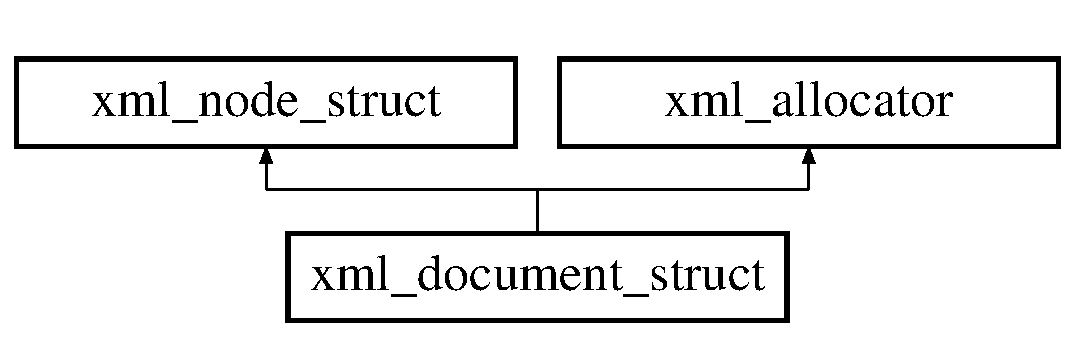
\includegraphics[height=2.000000cm]{structxml__document__struct}
\end{center}
\end{figure}
\subsection*{Public Member Functions}
\begin{DoxyCompactItemize}
\item 
\hyperlink{structxml__document__struct_aea3482436c20abd98ca063c3bd5dcfba}{xml\-\_\-document\-\_\-struct} (\hyperlink{structxml__memory__page}{xml\-\_\-memory\-\_\-page} $\ast$page)
\end{DoxyCompactItemize}
\subsection*{Data Fields}
\begin{DoxyCompactItemize}
\item 
const char\-\_\-t $\ast$ \hyperlink{structxml__document__struct_a120451f29b8cc2a82a3ecc926449ea0e}{buffer}
\end{DoxyCompactItemize}
\subsection*{Additional Inherited Members}


\subsection{Constructor \& Destructor Documentation}
\hypertarget{structxml__document__struct_aea3482436c20abd98ca063c3bd5dcfba}{\index{xml\-\_\-document\-\_\-struct@{xml\-\_\-document\-\_\-struct}!xml\-\_\-document\-\_\-struct@{xml\-\_\-document\-\_\-struct}}
\index{xml\-\_\-document\-\_\-struct@{xml\-\_\-document\-\_\-struct}!xml_document_struct@{xml\-\_\-document\-\_\-struct}}
\subsubsection[{xml\-\_\-document\-\_\-struct}]{\setlength{\rightskip}{0pt plus 5cm}xml\-\_\-document\-\_\-struct\-::xml\-\_\-document\-\_\-struct (
\begin{DoxyParamCaption}
\item[{{\bf xml\-\_\-memory\-\_\-page} $\ast$}]{page}
\end{DoxyParamCaption}
)\hspace{0.3cm}{\ttfamily [inline]}}}\label{structxml__document__struct_aea3482436c20abd98ca063c3bd5dcfba}

\begin{DoxyCode}
508                                                   : xml\_node\_struct(page, 
      \hyperlink{namespacepugi_a137e94a038e4ab0ada6477cf7f6153a9aab42ba83cf941f7297325eade205bf80}{node\_document}), \hyperlink{structxml__allocator_ad41b1a18595953aa71a470b45921c0fd}{xml\_allocator}(page), \hyperlink{structxml__document__struct_a120451f29b8cc2a82a3ecc926449ea0e}{buffer}(0)
509         \{
510         \}
\end{DoxyCode}


\subsection{Field Documentation}
\hypertarget{structxml__document__struct_a120451f29b8cc2a82a3ecc926449ea0e}{\index{xml\-\_\-document\-\_\-struct@{xml\-\_\-document\-\_\-struct}!buffer@{buffer}}
\index{buffer@{buffer}!xml_document_struct@{xml\-\_\-document\-\_\-struct}}
\subsubsection[{buffer}]{\setlength{\rightskip}{0pt plus 5cm}const char\-\_\-t$\ast$ xml\-\_\-document\-\_\-struct\-::buffer}}\label{structxml__document__struct_a120451f29b8cc2a82a3ecc926449ea0e}


The documentation for this struct was generated from the following file\-:\begin{DoxyCompactItemize}
\item 
Third\-Party/pugixml/\hyperlink{pugixml_8cpp}{pugixml.\-cpp}\end{DoxyCompactItemize}

\hypertarget{structxml__memory__management__function__storage}{\section{xml\-\_\-memory\-\_\-management\-\_\-function\-\_\-storage$<$ T $>$ Struct Template Reference}
\label{structxml__memory__management__function__storage}\index{xml\-\_\-memory\-\_\-management\-\_\-function\-\_\-storage$<$ T $>$@{xml\-\_\-memory\-\_\-management\-\_\-function\-\_\-storage$<$ T $>$}}
}
\subsection*{Static Public Attributes}
\begin{DoxyCompactItemize}
\item 
static allocation\-\_\-function \hyperlink{structxml__memory__management__function__storage_abb6865f8d07d27fd9273737c59f6e941}{allocate} = \hyperlink{pugixml_8cpp_a5c5a3cf417e46e0b3f5207fb9c6a5c18}{default\-\_\-allocate}
\item 
static deallocation\-\_\-function \hyperlink{structxml__memory__management__function__storage_a1c80a9a045ed6cfb90b17a178e4b3512}{deallocate} = \hyperlink{pugixml_8cpp_a04da64bb4806c0b7491d5d9d73d50100}{default\-\_\-deallocate}
\end{DoxyCompactItemize}


\subsection{Field Documentation}
\hypertarget{structxml__memory__management__function__storage_abb6865f8d07d27fd9273737c59f6e941}{\index{xml\-\_\-memory\-\_\-management\-\_\-function\-\_\-storage@{xml\-\_\-memory\-\_\-management\-\_\-function\-\_\-storage}!allocate@{allocate}}
\index{allocate@{allocate}!xml_memory_management_function_storage@{xml\-\_\-memory\-\_\-management\-\_\-function\-\_\-storage}}
\subsubsection[{allocate}]{\setlength{\rightskip}{0pt plus 5cm}template$<$typename T $>$ allocation\-\_\-function {\bf xml\-\_\-memory\-\_\-management\-\_\-function\-\_\-storage}$<$ T $>$\-::allocate = {\bf default\-\_\-allocate}\hspace{0.3cm}{\ttfamily [static]}}}\label{structxml__memory__management__function__storage_abb6865f8d07d27fd9273737c59f6e941}
\hypertarget{structxml__memory__management__function__storage_a1c80a9a045ed6cfb90b17a178e4b3512}{\index{xml\-\_\-memory\-\_\-management\-\_\-function\-\_\-storage@{xml\-\_\-memory\-\_\-management\-\_\-function\-\_\-storage}!deallocate@{deallocate}}
\index{deallocate@{deallocate}!xml_memory_management_function_storage@{xml\-\_\-memory\-\_\-management\-\_\-function\-\_\-storage}}
\subsubsection[{deallocate}]{\setlength{\rightskip}{0pt plus 5cm}template$<$typename T $>$ deallocation\-\_\-function {\bf xml\-\_\-memory\-\_\-management\-\_\-function\-\_\-storage}$<$ T $>$\-::deallocate = {\bf default\-\_\-deallocate}\hspace{0.3cm}{\ttfamily [static]}}}\label{structxml__memory__management__function__storage_a1c80a9a045ed6cfb90b17a178e4b3512}


The documentation for this struct was generated from the following file\-:\begin{DoxyCompactItemize}
\item 
Third\-Party/pugixml/\hyperlink{pugixml_8cpp}{pugixml.\-cpp}\end{DoxyCompactItemize}

\hypertarget{structxml__memory__page}{\section{xml\-\_\-memory\-\_\-page Struct Reference}
\label{structxml__memory__page}\index{xml\-\_\-memory\-\_\-page@{xml\-\_\-memory\-\_\-page}}
}
\subsection*{Static Public Member Functions}
\begin{DoxyCompactItemize}
\item 
static \hyperlink{structxml__memory__page}{xml\-\_\-memory\-\_\-page} $\ast$ \hyperlink{structxml__memory__page_ab425973f2abb4fa98ff077d88c0df11c}{construct} (void $\ast$\hyperlink{structxml__memory__page_ab51315db80e7f2a5afb87c56fedcd734}{memory})
\end{DoxyCompactItemize}
\subsection*{Data Fields}
\begin{DoxyCompactItemize}
\item 
\hyperlink{structxml__allocator}{xml\-\_\-allocator} $\ast$ \hyperlink{structxml__memory__page_adf8fa143123a842baa59b82fc3d83c3b}{allocator}
\item 
void $\ast$ \hyperlink{structxml__memory__page_ab51315db80e7f2a5afb87c56fedcd734}{memory}
\item 
\hyperlink{structxml__memory__page}{xml\-\_\-memory\-\_\-page} $\ast$ \hyperlink{structxml__memory__page_a014969b0e4a34a6cb24e9823791e60ab}{prev}
\item 
\hyperlink{structxml__memory__page}{xml\-\_\-memory\-\_\-page} $\ast$ \hyperlink{structxml__memory__page_a326a74e009af80219ea31bc65ed9e45e}{next}
\item 
size\-\_\-t \hyperlink{structxml__memory__page_a04780ddabc14b45baba3d1ded79d355a}{busy\-\_\-size}
\item 
size\-\_\-t \hyperlink{structxml__memory__page_ab4c29645546530a0e1938b53979890a8}{freed\-\_\-size}
\item 
char \hyperlink{structxml__memory__page_abd99ed1563aa66fb3573a9208452685c}{data} \mbox{[}1\mbox{]}
\end{DoxyCompactItemize}


\subsection{Member Function Documentation}
\hypertarget{structxml__memory__page_ab425973f2abb4fa98ff077d88c0df11c}{\index{xml\-\_\-memory\-\_\-page@{xml\-\_\-memory\-\_\-page}!construct@{construct}}
\index{construct@{construct}!xml_memory_page@{xml\-\_\-memory\-\_\-page}}
\subsubsection[{construct}]{\setlength{\rightskip}{0pt plus 5cm}static {\bf xml\-\_\-memory\-\_\-page}$\ast$ xml\-\_\-memory\-\_\-page\-::construct (
\begin{DoxyParamCaption}
\item[{void $\ast$}]{memory}
\end{DoxyParamCaption}
)\hspace{0.3cm}{\ttfamily [inline]}, {\ttfamily [static]}}}\label{structxml__memory__page_ab425973f2abb4fa98ff077d88c0df11c}

\begin{DoxyCode}
256         \{
257             \textcolor{keywordflow}{if} (!\hyperlink{structxml__memory__page_ab51315db80e7f2a5afb87c56fedcd734}{memory}) \textcolor{keywordflow}{return} 0; \textcolor{comment}{//$ redundant, left for performance}
258 
259             \hyperlink{structxml__memory__page}{xml\_memory\_page}* result = \textcolor{keyword}{static\_cast<}\hyperlink{structxml__memory__page}{xml\_memory\_page}*\textcolor{keyword}{>}(
      \hyperlink{structxml__memory__page_ab51315db80e7f2a5afb87c56fedcd734}{memory});
260 
261             result->\hyperlink{structxml__memory__page_adf8fa143123a842baa59b82fc3d83c3b}{allocator} = 0;
262             result->\hyperlink{structxml__memory__page_ab51315db80e7f2a5afb87c56fedcd734}{memory} = 0;
263             result->\hyperlink{structxml__memory__page_a014969b0e4a34a6cb24e9823791e60ab}{prev} = 0;
264             result->\hyperlink{structxml__memory__page_a326a74e009af80219ea31bc65ed9e45e}{next} = 0;
265             result->\hyperlink{structxml__memory__page_a04780ddabc14b45baba3d1ded79d355a}{busy\_size} = 0;
266             result->\hyperlink{structxml__memory__page_ab4c29645546530a0e1938b53979890a8}{freed\_size} = 0;
267 
268             \textcolor{keywordflow}{return} result;
269         \}
\end{DoxyCode}


\subsection{Field Documentation}
\hypertarget{structxml__memory__page_adf8fa143123a842baa59b82fc3d83c3b}{\index{xml\-\_\-memory\-\_\-page@{xml\-\_\-memory\-\_\-page}!allocator@{allocator}}
\index{allocator@{allocator}!xml_memory_page@{xml\-\_\-memory\-\_\-page}}
\subsubsection[{allocator}]{\setlength{\rightskip}{0pt plus 5cm}{\bf xml\-\_\-allocator}$\ast$ xml\-\_\-memory\-\_\-page\-::allocator}}\label{structxml__memory__page_adf8fa143123a842baa59b82fc3d83c3b}
\hypertarget{structxml__memory__page_a04780ddabc14b45baba3d1ded79d355a}{\index{xml\-\_\-memory\-\_\-page@{xml\-\_\-memory\-\_\-page}!busy\-\_\-size@{busy\-\_\-size}}
\index{busy\-\_\-size@{busy\-\_\-size}!xml_memory_page@{xml\-\_\-memory\-\_\-page}}
\subsubsection[{busy\-\_\-size}]{\setlength{\rightskip}{0pt plus 5cm}size\-\_\-t xml\-\_\-memory\-\_\-page\-::busy\-\_\-size}}\label{structxml__memory__page_a04780ddabc14b45baba3d1ded79d355a}
\hypertarget{structxml__memory__page_abd99ed1563aa66fb3573a9208452685c}{\index{xml\-\_\-memory\-\_\-page@{xml\-\_\-memory\-\_\-page}!data@{data}}
\index{data@{data}!xml_memory_page@{xml\-\_\-memory\-\_\-page}}
\subsubsection[{data}]{\setlength{\rightskip}{0pt plus 5cm}char xml\-\_\-memory\-\_\-page\-::data\mbox{[}1\mbox{]}}}\label{structxml__memory__page_abd99ed1563aa66fb3573a9208452685c}
\hypertarget{structxml__memory__page_ab4c29645546530a0e1938b53979890a8}{\index{xml\-\_\-memory\-\_\-page@{xml\-\_\-memory\-\_\-page}!freed\-\_\-size@{freed\-\_\-size}}
\index{freed\-\_\-size@{freed\-\_\-size}!xml_memory_page@{xml\-\_\-memory\-\_\-page}}
\subsubsection[{freed\-\_\-size}]{\setlength{\rightskip}{0pt plus 5cm}size\-\_\-t xml\-\_\-memory\-\_\-page\-::freed\-\_\-size}}\label{structxml__memory__page_ab4c29645546530a0e1938b53979890a8}
\hypertarget{structxml__memory__page_ab51315db80e7f2a5afb87c56fedcd734}{\index{xml\-\_\-memory\-\_\-page@{xml\-\_\-memory\-\_\-page}!memory@{memory}}
\index{memory@{memory}!xml_memory_page@{xml\-\_\-memory\-\_\-page}}
\subsubsection[{memory}]{\setlength{\rightskip}{0pt plus 5cm}void$\ast$ xml\-\_\-memory\-\_\-page\-::memory}}\label{structxml__memory__page_ab51315db80e7f2a5afb87c56fedcd734}
\hypertarget{structxml__memory__page_a326a74e009af80219ea31bc65ed9e45e}{\index{xml\-\_\-memory\-\_\-page@{xml\-\_\-memory\-\_\-page}!next@{next}}
\index{next@{next}!xml_memory_page@{xml\-\_\-memory\-\_\-page}}
\subsubsection[{next}]{\setlength{\rightskip}{0pt plus 5cm}{\bf xml\-\_\-memory\-\_\-page}$\ast$ xml\-\_\-memory\-\_\-page\-::next}}\label{structxml__memory__page_a326a74e009af80219ea31bc65ed9e45e}
\hypertarget{structxml__memory__page_a014969b0e4a34a6cb24e9823791e60ab}{\index{xml\-\_\-memory\-\_\-page@{xml\-\_\-memory\-\_\-page}!prev@{prev}}
\index{prev@{prev}!xml_memory_page@{xml\-\_\-memory\-\_\-page}}
\subsubsection[{prev}]{\setlength{\rightskip}{0pt plus 5cm}{\bf xml\-\_\-memory\-\_\-page}$\ast$ xml\-\_\-memory\-\_\-page\-::prev}}\label{structxml__memory__page_a014969b0e4a34a6cb24e9823791e60ab}


The documentation for this struct was generated from the following file\-:\begin{DoxyCompactItemize}
\item 
Third\-Party/pugixml/\hyperlink{pugixml_8cpp}{pugixml.\-cpp}\end{DoxyCompactItemize}

\hypertarget{structxml__memory__string__header}{\section{xml\-\_\-memory\-\_\-string\-\_\-header Struct Reference}
\label{structxml__memory__string__header}\index{xml\-\_\-memory\-\_\-string\-\_\-header@{xml\-\_\-memory\-\_\-string\-\_\-header}}
}
\subsection*{Data Fields}
\begin{DoxyCompactItemize}
\item 
uint16\-\_\-t \hyperlink{structxml__memory__string__header_a0cc274672f1263f73eeb6bf839bf96ee}{page\-\_\-offset}
\item 
uint16\-\_\-t \hyperlink{structxml__memory__string__header_abbb48a709081e6610dffad322499e3f7}{full\-\_\-size}
\end{DoxyCompactItemize}


\subsection{Field Documentation}
\hypertarget{structxml__memory__string__header_abbb48a709081e6610dffad322499e3f7}{\index{xml\-\_\-memory\-\_\-string\-\_\-header@{xml\-\_\-memory\-\_\-string\-\_\-header}!full\-\_\-size@{full\-\_\-size}}
\index{full\-\_\-size@{full\-\_\-size}!xml_memory_string_header@{xml\-\_\-memory\-\_\-string\-\_\-header}}
\subsubsection[{full\-\_\-size}]{\setlength{\rightskip}{0pt plus 5cm}uint16\-\_\-t xml\-\_\-memory\-\_\-string\-\_\-header\-::full\-\_\-size}}\label{structxml__memory__string__header_abbb48a709081e6610dffad322499e3f7}
\hypertarget{structxml__memory__string__header_a0cc274672f1263f73eeb6bf839bf96ee}{\index{xml\-\_\-memory\-\_\-string\-\_\-header@{xml\-\_\-memory\-\_\-string\-\_\-header}!page\-\_\-offset@{page\-\_\-offset}}
\index{page\-\_\-offset@{page\-\_\-offset}!xml_memory_string_header@{xml\-\_\-memory\-\_\-string\-\_\-header}}
\subsubsection[{page\-\_\-offset}]{\setlength{\rightskip}{0pt plus 5cm}uint16\-\_\-t xml\-\_\-memory\-\_\-string\-\_\-header\-::page\-\_\-offset}}\label{structxml__memory__string__header_a0cc274672f1263f73eeb6bf839bf96ee}


The documentation for this struct was generated from the following file\-:\begin{DoxyCompactItemize}
\item 
Third\-Party/pugixml/\hyperlink{pugixml_8cpp}{pugixml.\-cpp}\end{DoxyCompactItemize}

\hypertarget{classpugi_1_1xml__named__node__iterator}{\section{pugi\-:\-:xml\-\_\-named\-\_\-node\-\_\-iterator Class Reference}
\label{classpugi_1_1xml__named__node__iterator}\index{pugi\-::xml\-\_\-named\-\_\-node\-\_\-iterator@{pugi\-::xml\-\_\-named\-\_\-node\-\_\-iterator}}
}


{\ttfamily \#include $<$pugixml.\-hpp$>$}

\subsection*{Public Types}
\begin{DoxyCompactItemize}
\item 
typedef ptrdiff\-\_\-t \hyperlink{classpugi_1_1xml__named__node__iterator_a18fa0d610fea4d64271729abc0e28849}{difference\-\_\-type}
\item 
typedef \hyperlink{classpugi_1_1xml__node}{xml\-\_\-node} \hyperlink{classpugi_1_1xml__named__node__iterator_a8d98d8218ea9740ceb990ef2c1a456e2}{value\-\_\-type}
\item 
typedef \hyperlink{classpugi_1_1xml__node}{xml\-\_\-node} $\ast$ \hyperlink{classpugi_1_1xml__named__node__iterator_aebf72c68ded20cf483a10c6b94aa3f57}{pointer}
\item 
typedef \hyperlink{classpugi_1_1xml__node}{xml\-\_\-node} \& \hyperlink{classpugi_1_1xml__named__node__iterator_a1c338c7a2aefe04b83f746a963df808b}{reference}
\item 
typedef std\-::forward\-\_\-iterator\-\_\-tag \hyperlink{classpugi_1_1xml__named__node__iterator_a8d3aa9d72f7b79c82f40933b3b0db9cd}{iterator\-\_\-category}
\end{DoxyCompactItemize}
\subsection*{Public Member Functions}
\begin{DoxyCompactItemize}
\item 
\hyperlink{classpugi_1_1xml__named__node__iterator_a0cf8880a79c3723159d91ef025961bea}{xml\-\_\-named\-\_\-node\-\_\-iterator} ()
\item 
\hyperlink{classpugi_1_1xml__named__node__iterator_a900cdc6c175bcb56b1c66c7c05d2202f}{xml\-\_\-named\-\_\-node\-\_\-iterator} (const \hyperlink{classpugi_1_1xml__node}{xml\-\_\-node} \&node, const \hyperlink{namespacepugi_aef5a7a62cba0507542220ea15afe39df}{char\-\_\-t} $\ast$name)
\item 
bool \hyperlink{classpugi_1_1xml__named__node__iterator_a49533305b71d21a160dda111a2ed9956}{operator==} (const \hyperlink{classpugi_1_1xml__named__node__iterator}{xml\-\_\-named\-\_\-node\-\_\-iterator} \&rhs) const 
\item 
bool \hyperlink{classpugi_1_1xml__named__node__iterator_a3f625995e15f1b5debecdb9fb618c9d9}{operator!=} (const \hyperlink{classpugi_1_1xml__named__node__iterator}{xml\-\_\-named\-\_\-node\-\_\-iterator} \&rhs) const 
\item 
\hyperlink{classpugi_1_1xml__node}{xml\-\_\-node} \& \hyperlink{classpugi_1_1xml__named__node__iterator_a382a1fe2474c25b47d96dd901e3add8a}{operator$\ast$} () const 
\item 
\hyperlink{classpugi_1_1xml__node}{xml\-\_\-node} $\ast$ \hyperlink{classpugi_1_1xml__named__node__iterator_a9fa4ca35803bfd50c61d369241a3da4a}{operator-\/$>$} () const 
\item 
const \hyperlink{classpugi_1_1xml__named__node__iterator}{xml\-\_\-named\-\_\-node\-\_\-iterator} \& \hyperlink{classpugi_1_1xml__named__node__iterator_ae076ec9c8414c5444ce6e4db5052ccef}{operator++} ()
\item 
\hyperlink{classpugi_1_1xml__named__node__iterator}{xml\-\_\-named\-\_\-node\-\_\-iterator} \hyperlink{classpugi_1_1xml__named__node__iterator_a41e2afe0ee62a2d06d0694052277e1f9}{operator++} (int)
\end{DoxyCompactItemize}


\subsection{Member Typedef Documentation}
\hypertarget{classpugi_1_1xml__named__node__iterator_a18fa0d610fea4d64271729abc0e28849}{\index{pugi\-::xml\-\_\-named\-\_\-node\-\_\-iterator@{pugi\-::xml\-\_\-named\-\_\-node\-\_\-iterator}!difference\-\_\-type@{difference\-\_\-type}}
\index{difference\-\_\-type@{difference\-\_\-type}!pugi::xml_named_node_iterator@{pugi\-::xml\-\_\-named\-\_\-node\-\_\-iterator}}
\subsubsection[{difference\-\_\-type}]{\setlength{\rightskip}{0pt plus 5cm}typedef ptrdiff\-\_\-t {\bf pugi\-::xml\-\_\-named\-\_\-node\-\_\-iterator\-::difference\-\_\-type}}}\label{classpugi_1_1xml__named__node__iterator_a18fa0d610fea4d64271729abc0e28849}
\hypertarget{classpugi_1_1xml__named__node__iterator_a8d3aa9d72f7b79c82f40933b3b0db9cd}{\index{pugi\-::xml\-\_\-named\-\_\-node\-\_\-iterator@{pugi\-::xml\-\_\-named\-\_\-node\-\_\-iterator}!iterator\-\_\-category@{iterator\-\_\-category}}
\index{iterator\-\_\-category@{iterator\-\_\-category}!pugi::xml_named_node_iterator@{pugi\-::xml\-\_\-named\-\_\-node\-\_\-iterator}}
\subsubsection[{iterator\-\_\-category}]{\setlength{\rightskip}{0pt plus 5cm}typedef std\-::forward\-\_\-iterator\-\_\-tag {\bf pugi\-::xml\-\_\-named\-\_\-node\-\_\-iterator\-::iterator\-\_\-category}}}\label{classpugi_1_1xml__named__node__iterator_a8d3aa9d72f7b79c82f40933b3b0db9cd}
\hypertarget{classpugi_1_1xml__named__node__iterator_aebf72c68ded20cf483a10c6b94aa3f57}{\index{pugi\-::xml\-\_\-named\-\_\-node\-\_\-iterator@{pugi\-::xml\-\_\-named\-\_\-node\-\_\-iterator}!pointer@{pointer}}
\index{pointer@{pointer}!pugi::xml_named_node_iterator@{pugi\-::xml\-\_\-named\-\_\-node\-\_\-iterator}}
\subsubsection[{pointer}]{\setlength{\rightskip}{0pt plus 5cm}typedef {\bf xml\-\_\-node}$\ast$ {\bf pugi\-::xml\-\_\-named\-\_\-node\-\_\-iterator\-::pointer}}}\label{classpugi_1_1xml__named__node__iterator_aebf72c68ded20cf483a10c6b94aa3f57}
\hypertarget{classpugi_1_1xml__named__node__iterator_a1c338c7a2aefe04b83f746a963df808b}{\index{pugi\-::xml\-\_\-named\-\_\-node\-\_\-iterator@{pugi\-::xml\-\_\-named\-\_\-node\-\_\-iterator}!reference@{reference}}
\index{reference@{reference}!pugi::xml_named_node_iterator@{pugi\-::xml\-\_\-named\-\_\-node\-\_\-iterator}}
\subsubsection[{reference}]{\setlength{\rightskip}{0pt plus 5cm}typedef {\bf xml\-\_\-node}\& {\bf pugi\-::xml\-\_\-named\-\_\-node\-\_\-iterator\-::reference}}}\label{classpugi_1_1xml__named__node__iterator_a1c338c7a2aefe04b83f746a963df808b}
\hypertarget{classpugi_1_1xml__named__node__iterator_a8d98d8218ea9740ceb990ef2c1a456e2}{\index{pugi\-::xml\-\_\-named\-\_\-node\-\_\-iterator@{pugi\-::xml\-\_\-named\-\_\-node\-\_\-iterator}!value\-\_\-type@{value\-\_\-type}}
\index{value\-\_\-type@{value\-\_\-type}!pugi::xml_named_node_iterator@{pugi\-::xml\-\_\-named\-\_\-node\-\_\-iterator}}
\subsubsection[{value\-\_\-type}]{\setlength{\rightskip}{0pt plus 5cm}typedef {\bf xml\-\_\-node} {\bf pugi\-::xml\-\_\-named\-\_\-node\-\_\-iterator\-::value\-\_\-type}}}\label{classpugi_1_1xml__named__node__iterator_a8d98d8218ea9740ceb990ef2c1a456e2}


\subsection{Constructor \& Destructor Documentation}
\hypertarget{classpugi_1_1xml__named__node__iterator_a0cf8880a79c3723159d91ef025961bea}{\index{pugi\-::xml\-\_\-named\-\_\-node\-\_\-iterator@{pugi\-::xml\-\_\-named\-\_\-node\-\_\-iterator}!xml\-\_\-named\-\_\-node\-\_\-iterator@{xml\-\_\-named\-\_\-node\-\_\-iterator}}
\index{xml\-\_\-named\-\_\-node\-\_\-iterator@{xml\-\_\-named\-\_\-node\-\_\-iterator}!pugi::xml_named_node_iterator@{pugi\-::xml\-\_\-named\-\_\-node\-\_\-iterator}}
\subsubsection[{xml\-\_\-named\-\_\-node\-\_\-iterator}]{\setlength{\rightskip}{0pt plus 5cm}{\bf P\-U\-G\-I\-\_\-\-\_\-\-F\-N} pugi\-::xml\-\_\-named\-\_\-node\-\_\-iterator\-::xml\-\_\-named\-\_\-node\-\_\-iterator (
\begin{DoxyParamCaption}
{}
\end{DoxyParamCaption}
)}}\label{classpugi_1_1xml__named__node__iterator_a0cf8880a79c3723159d91ef025961bea}

\begin{DoxyCode}
5022                                                              : \_name(0)
5023     \{
5024     \}
\end{DoxyCode}
\hypertarget{classpugi_1_1xml__named__node__iterator_a900cdc6c175bcb56b1c66c7c05d2202f}{\index{pugi\-::xml\-\_\-named\-\_\-node\-\_\-iterator@{pugi\-::xml\-\_\-named\-\_\-node\-\_\-iterator}!xml\-\_\-named\-\_\-node\-\_\-iterator@{xml\-\_\-named\-\_\-node\-\_\-iterator}}
\index{xml\-\_\-named\-\_\-node\-\_\-iterator@{xml\-\_\-named\-\_\-node\-\_\-iterator}!pugi::xml_named_node_iterator@{pugi\-::xml\-\_\-named\-\_\-node\-\_\-iterator}}
\subsubsection[{xml\-\_\-named\-\_\-node\-\_\-iterator}]{\setlength{\rightskip}{0pt plus 5cm}{\bf P\-U\-G\-I\-\_\-\-\_\-\-F\-N} pugi\-::xml\-\_\-named\-\_\-node\-\_\-iterator\-::xml\-\_\-named\-\_\-node\-\_\-iterator (
\begin{DoxyParamCaption}
\item[{const {\bf xml\-\_\-node} \&}]{node, }
\item[{const {\bf char\-\_\-t} $\ast$}]{name}
\end{DoxyParamCaption}
)}}\label{classpugi_1_1xml__named__node__iterator_a900cdc6c175bcb56b1c66c7c05d2202f}

\begin{DoxyCode}
5026                                                                                                      : 
      \_node(node), \_name(name)
5027     \{
5028     \}
\end{DoxyCode}


\subsection{Member Function Documentation}
\hypertarget{classpugi_1_1xml__named__node__iterator_a3f625995e15f1b5debecdb9fb618c9d9}{\index{pugi\-::xml\-\_\-named\-\_\-node\-\_\-iterator@{pugi\-::xml\-\_\-named\-\_\-node\-\_\-iterator}!operator!=@{operator!=}}
\index{operator!=@{operator!=}!pugi::xml_named_node_iterator@{pugi\-::xml\-\_\-named\-\_\-node\-\_\-iterator}}
\subsubsection[{operator!=}]{\setlength{\rightskip}{0pt plus 5cm}{\bf P\-U\-G\-I\-\_\-\-\_\-\-F\-N} bool pugi\-::xml\-\_\-named\-\_\-node\-\_\-iterator\-::operator!= (
\begin{DoxyParamCaption}
\item[{const {\bf xml\-\_\-named\-\_\-node\-\_\-iterator} \&}]{rhs}
\end{DoxyParamCaption}
) const}}\label{classpugi_1_1xml__named__node__iterator_a3f625995e15f1b5debecdb9fb618c9d9}

\begin{DoxyCode}
5036     \{
5037         \textcolor{keywordflow}{return} \_node != rhs.\_node;
5038     \}
\end{DoxyCode}
\hypertarget{classpugi_1_1xml__named__node__iterator_a382a1fe2474c25b47d96dd901e3add8a}{\index{pugi\-::xml\-\_\-named\-\_\-node\-\_\-iterator@{pugi\-::xml\-\_\-named\-\_\-node\-\_\-iterator}!operator$\ast$@{operator$\ast$}}
\index{operator$\ast$@{operator$\ast$}!pugi::xml_named_node_iterator@{pugi\-::xml\-\_\-named\-\_\-node\-\_\-iterator}}
\subsubsection[{operator$\ast$}]{\setlength{\rightskip}{0pt plus 5cm}{\bf P\-U\-G\-I\-\_\-\-\_\-\-F\-N} {\bf xml\-\_\-node} \& pugi\-::xml\-\_\-named\-\_\-node\-\_\-iterator\-::operator$\ast$ (
\begin{DoxyParamCaption}
{}
\end{DoxyParamCaption}
) const}}\label{classpugi_1_1xml__named__node__iterator_a382a1fe2474c25b47d96dd901e3add8a}

\begin{DoxyCode}
5041     \{
5042         assert(\_node.\hyperlink{classpugi_1_1xml__node_a45a5b342de1e37a60565f7693f03cc08}{\_root});
5043         \textcolor{keywordflow}{return} \_node;
5044     \}
\end{DoxyCode}
\hypertarget{classpugi_1_1xml__named__node__iterator_ae076ec9c8414c5444ce6e4db5052ccef}{\index{pugi\-::xml\-\_\-named\-\_\-node\-\_\-iterator@{pugi\-::xml\-\_\-named\-\_\-node\-\_\-iterator}!operator++@{operator++}}
\index{operator++@{operator++}!pugi::xml_named_node_iterator@{pugi\-::xml\-\_\-named\-\_\-node\-\_\-iterator}}
\subsubsection[{operator++}]{\setlength{\rightskip}{0pt plus 5cm}{\bf P\-U\-G\-I\-\_\-\-\_\-\-F\-N} const {\bf xml\-\_\-named\-\_\-node\-\_\-iterator} \& pugi\-::xml\-\_\-named\-\_\-node\-\_\-iterator\-::operator++ (
\begin{DoxyParamCaption}
{}
\end{DoxyParamCaption}
)}}\label{classpugi_1_1xml__named__node__iterator_ae076ec9c8414c5444ce6e4db5052ccef}

\begin{DoxyCode}
5053     \{
5054         assert(\_node.\hyperlink{classpugi_1_1xml__node_a45a5b342de1e37a60565f7693f03cc08}{\_root});
5055         \_node = \_node.\hyperlink{classpugi_1_1xml__node_a713159ab981fb3f0a325434106dc94f5}{next\_sibling}(\_name);
5056         \textcolor{keywordflow}{return} *\textcolor{keyword}{this};
5057     \}
\end{DoxyCode}
\hypertarget{classpugi_1_1xml__named__node__iterator_a41e2afe0ee62a2d06d0694052277e1f9}{\index{pugi\-::xml\-\_\-named\-\_\-node\-\_\-iterator@{pugi\-::xml\-\_\-named\-\_\-node\-\_\-iterator}!operator++@{operator++}}
\index{operator++@{operator++}!pugi::xml_named_node_iterator@{pugi\-::xml\-\_\-named\-\_\-node\-\_\-iterator}}
\subsubsection[{operator++}]{\setlength{\rightskip}{0pt plus 5cm}{\bf P\-U\-G\-I\-\_\-\-\_\-\-F\-N} {\bf xml\-\_\-named\-\_\-node\-\_\-iterator} pugi\-::xml\-\_\-named\-\_\-node\-\_\-iterator\-::operator++ (
\begin{DoxyParamCaption}
\item[{int}]{}
\end{DoxyParamCaption}
)}}\label{classpugi_1_1xml__named__node__iterator_a41e2afe0ee62a2d06d0694052277e1f9}

\begin{DoxyCode}
5060     \{
5061         \hyperlink{classpugi_1_1xml__named__node__iterator_a0cf8880a79c3723159d91ef025961bea}{xml\_named\_node\_iterator} temp = *\textcolor{keyword}{this};
5062         ++*\textcolor{keyword}{this};
5063         \textcolor{keywordflow}{return} temp;
5064     \}
\end{DoxyCode}
\hypertarget{classpugi_1_1xml__named__node__iterator_a9fa4ca35803bfd50c61d369241a3da4a}{\index{pugi\-::xml\-\_\-named\-\_\-node\-\_\-iterator@{pugi\-::xml\-\_\-named\-\_\-node\-\_\-iterator}!operator-\/$>$@{operator-\/$>$}}
\index{operator-\/$>$@{operator-\/$>$}!pugi::xml_named_node_iterator@{pugi\-::xml\-\_\-named\-\_\-node\-\_\-iterator}}
\subsubsection[{operator-\/$>$}]{\setlength{\rightskip}{0pt plus 5cm}{\bf P\-U\-G\-I\-\_\-\-\_\-\-F\-N} {\bf xml\-\_\-node} $\ast$ pugi\-::xml\-\_\-named\-\_\-node\-\_\-iterator\-::operator-\/$>$ (
\begin{DoxyParamCaption}
{}
\end{DoxyParamCaption}
) const}}\label{classpugi_1_1xml__named__node__iterator_a9fa4ca35803bfd50c61d369241a3da4a}

\begin{DoxyCode}
5047     \{
5048         assert(\_node.\hyperlink{classpugi_1_1xml__node_a45a5b342de1e37a60565f7693f03cc08}{\_root});
5049         \textcolor{keywordflow}{return} \textcolor{keyword}{const\_cast<}xml\_node*\textcolor{keyword}{>}(&\_node); \textcolor{comment}{// BCC32 workaround}
5050     \}
\end{DoxyCode}
\hypertarget{classpugi_1_1xml__named__node__iterator_a49533305b71d21a160dda111a2ed9956}{\index{pugi\-::xml\-\_\-named\-\_\-node\-\_\-iterator@{pugi\-::xml\-\_\-named\-\_\-node\-\_\-iterator}!operator==@{operator==}}
\index{operator==@{operator==}!pugi::xml_named_node_iterator@{pugi\-::xml\-\_\-named\-\_\-node\-\_\-iterator}}
\subsubsection[{operator==}]{\setlength{\rightskip}{0pt plus 5cm}{\bf P\-U\-G\-I\-\_\-\-\_\-\-F\-N} bool pugi\-::xml\-\_\-named\-\_\-node\-\_\-iterator\-::operator== (
\begin{DoxyParamCaption}
\item[{const {\bf xml\-\_\-named\-\_\-node\-\_\-iterator} \&}]{rhs}
\end{DoxyParamCaption}
) const}}\label{classpugi_1_1xml__named__node__iterator_a49533305b71d21a160dda111a2ed9956}

\begin{DoxyCode}
5031     \{
5032         \textcolor{keywordflow}{return} \_node == rhs.\_node;
5033     \}
\end{DoxyCode}


The documentation for this class was generated from the following files\-:\begin{DoxyCompactItemize}
\item 
Third\-Party/pugixml/\hyperlink{pugixml_8hpp}{pugixml.\-hpp}\item 
Third\-Party/pugixml/\hyperlink{pugixml_8cpp}{pugixml.\-cpp}\end{DoxyCompactItemize}

\hypertarget{classpugi_1_1xml__node}{\section{pugi\-:\-:xml\-\_\-node Class Reference}
\label{classpugi_1_1xml__node}\index{pugi\-::xml\-\_\-node@{pugi\-::xml\-\_\-node}}
}


{\ttfamily \#include $<$pugixml.\-hpp$>$}

Inheritance diagram for pugi\-:\-:xml\-\_\-node\-:\begin{figure}[H]
\begin{center}
\leavevmode
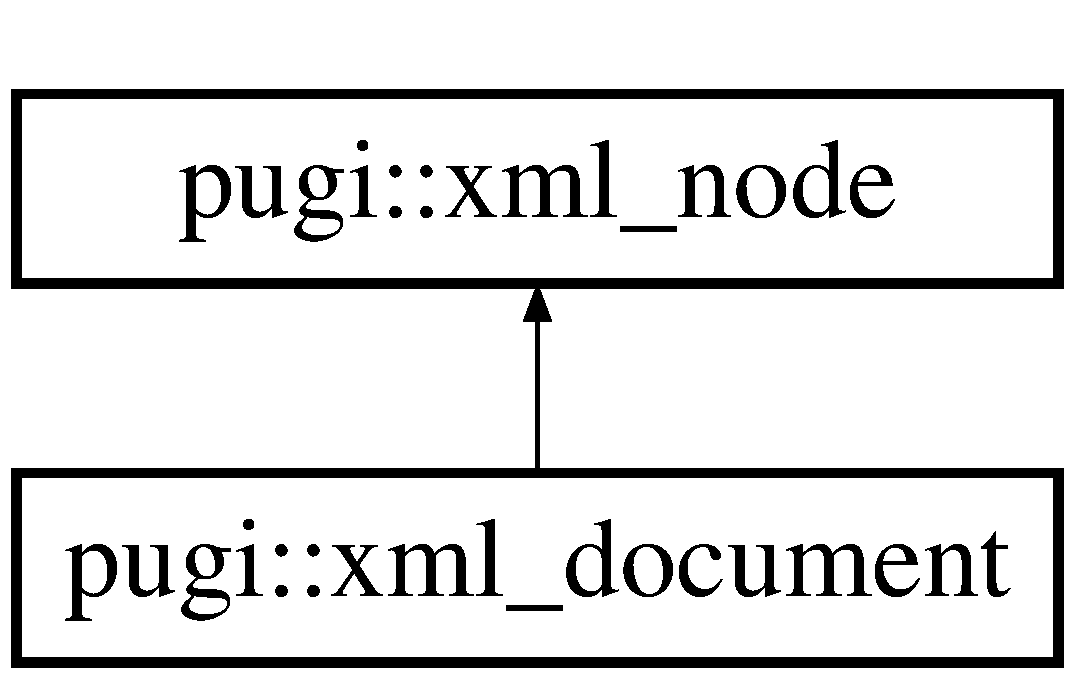
\includegraphics[height=2.000000cm]{classpugi_1_1xml__node}
\end{center}
\end{figure}
\subsection*{Public Types}
\begin{DoxyCompactItemize}
\item 
typedef \hyperlink{classpugi_1_1xml__node__iterator}{xml\-\_\-node\-\_\-iterator} \hyperlink{classpugi_1_1xml__node_ae053ea39add5a64de584f7a81212e388}{iterator}
\item 
typedef \hyperlink{classpugi_1_1xml__attribute__iterator}{xml\-\_\-attribute\-\_\-iterator} \hyperlink{classpugi_1_1xml__node_a9084f97350ffc64af1eaf7c17c57f4ba}{attribute\-\_\-iterator}
\end{DoxyCompactItemize}
\subsection*{Public Member Functions}
\begin{DoxyCompactItemize}
\item 
\hyperlink{classpugi_1_1xml__node_a36ec0eb8b399d71f6b55be0e181c69f9}{xml\-\_\-node} ()
\item 
\hyperlink{classpugi_1_1xml__node_afc9b1ed8891dfed9ce5ab5288a9ad4a1}{xml\-\_\-node} (\hyperlink{structpugi_1_1xml__node__struct}{xml\-\_\-node\-\_\-struct} $\ast$p)
\item 
\hyperlink{classpugi_1_1xml__node_af30001c73a3454a1e3794a850d3963c0}{operator unspecified\-\_\-bool\-\_\-type} () const 
\item 
bool \hyperlink{classpugi_1_1xml__node_a03c028fd83e07cda3f433f9eea3466ff}{operator!} () const 
\item 
bool \hyperlink{classpugi_1_1xml__node_aaf46fa45a1a117ca95867f37ade363c2}{operator==} (const \hyperlink{classpugi_1_1xml__node}{xml\-\_\-node} \&r) const 
\item 
bool \hyperlink{classpugi_1_1xml__node_aa31095e51422a8a11b8d4832e0db71ed}{operator!=} (const \hyperlink{classpugi_1_1xml__node}{xml\-\_\-node} \&r) const 
\item 
bool \hyperlink{classpugi_1_1xml__node_a2a57731a8d90392f88febf551bd5a924}{operator$<$} (const \hyperlink{classpugi_1_1xml__node}{xml\-\_\-node} \&r) const 
\item 
bool \hyperlink{classpugi_1_1xml__node_a983e49938a893181fd8cc905c4c67f64}{operator$>$} (const \hyperlink{classpugi_1_1xml__node}{xml\-\_\-node} \&r) const 
\item 
bool \hyperlink{classpugi_1_1xml__node_a09568e579d8c1b6bff12594bfb4246b6}{operator$<$=} (const \hyperlink{classpugi_1_1xml__node}{xml\-\_\-node} \&r) const 
\item 
bool \hyperlink{classpugi_1_1xml__node_a8c89c4333fdd22f19714a945895d2e39}{operator$>$=} (const \hyperlink{classpugi_1_1xml__node}{xml\-\_\-node} \&r) const 
\item 
bool \hyperlink{classpugi_1_1xml__node_a2c416c45fcd27a9cf4e7914d560a0cc4}{empty} () const 
\item 
\hyperlink{namespacepugi_a137e94a038e4ab0ada6477cf7f6153a9}{xml\-\_\-node\-\_\-type} \hyperlink{classpugi_1_1xml__node_ab881e8c41edc84bf7507591d1ad8ead4}{type} () const 
\item 
const \hyperlink{namespacepugi_aef5a7a62cba0507542220ea15afe39df}{char\-\_\-t} $\ast$ \hyperlink{classpugi_1_1xml__node_ac765caace42ecf252d90aea81e09df57}{name} () const 
\item 
const \hyperlink{namespacepugi_aef5a7a62cba0507542220ea15afe39df}{char\-\_\-t} $\ast$ \hyperlink{classpugi_1_1xml__node_a3e7e935a101432fd4f6dcaf6bfb495d4}{value} () const 
\item 
\hyperlink{classpugi_1_1xml__attribute}{xml\-\_\-attribute} \hyperlink{classpugi_1_1xml__node_ac53e177390f1f73e6cef4f5be3ecaa9d}{first\-\_\-attribute} () const 
\item 
\hyperlink{classpugi_1_1xml__attribute}{xml\-\_\-attribute} \hyperlink{classpugi_1_1xml__node_a10695e006b24e726ba313d5554086802}{last\-\_\-attribute} () const 
\item 
\hyperlink{classpugi_1_1xml__node}{xml\-\_\-node} \hyperlink{classpugi_1_1xml__node_a71641cb34be57df1b25e2df7eac31f00}{first\-\_\-child} () const 
\item 
\hyperlink{classpugi_1_1xml__node}{xml\-\_\-node} \hyperlink{classpugi_1_1xml__node_a076b2868a97458d5abeeec9e6c433244}{last\-\_\-child} () const 
\item 
\hyperlink{classpugi_1_1xml__node}{xml\-\_\-node} \hyperlink{classpugi_1_1xml__node_a713159ab981fb3f0a325434106dc94f5}{next\-\_\-sibling} () const 
\item 
\hyperlink{classpugi_1_1xml__node}{xml\-\_\-node} \hyperlink{classpugi_1_1xml__node_a367e7e2c78a3870aad7ad3831da7c0fa}{previous\-\_\-sibling} () const 
\item 
\hyperlink{classpugi_1_1xml__node}{xml\-\_\-node} \hyperlink{classpugi_1_1xml__node_a5c7a1b2ec89d59afa1028e9c5fc25640}{parent} () const 
\item 
\hyperlink{classpugi_1_1xml__node}{xml\-\_\-node} \hyperlink{classpugi_1_1xml__node_a713b60fd5cddd5d8671dd76b1457e6eb}{root} () const 
\item 
\hyperlink{classpugi_1_1xml__text}{xml\-\_\-text} \hyperlink{classpugi_1_1xml__node_aafe1c1c7cd27f3c9c758b517abc7886a}{text} () const 
\item 
\hyperlink{classpugi_1_1xml__node}{xml\-\_\-node} \hyperlink{classpugi_1_1xml__node_af3aa192b114a289640110c9e4da020ca}{child} (const \hyperlink{namespacepugi_aef5a7a62cba0507542220ea15afe39df}{char\-\_\-t} $\ast$\hyperlink{classpugi_1_1xml__node_ac765caace42ecf252d90aea81e09df57}{name}) const 
\item 
\hyperlink{classpugi_1_1xml__attribute}{xml\-\_\-attribute} \hyperlink{classpugi_1_1xml__node_a19fc1a285c0f751f52c0e151a727de97}{attribute} (const \hyperlink{namespacepugi_aef5a7a62cba0507542220ea15afe39df}{char\-\_\-t} $\ast$\hyperlink{classpugi_1_1xml__node_ac765caace42ecf252d90aea81e09df57}{name}) const 
\item 
\hyperlink{classpugi_1_1xml__node}{xml\-\_\-node} \hyperlink{classpugi_1_1xml__node_a51a25d1e6f2315b65a1f969126cbc612}{next\-\_\-sibling} (const \hyperlink{namespacepugi_aef5a7a62cba0507542220ea15afe39df}{char\-\_\-t} $\ast$\hyperlink{classpugi_1_1xml__node_ac765caace42ecf252d90aea81e09df57}{name}) const 
\item 
\hyperlink{classpugi_1_1xml__node}{xml\-\_\-node} \hyperlink{classpugi_1_1xml__node_a311405d1ee4a564071a5f44b476b05f7}{previous\-\_\-sibling} (const \hyperlink{namespacepugi_aef5a7a62cba0507542220ea15afe39df}{char\-\_\-t} $\ast$\hyperlink{classpugi_1_1xml__node_ac765caace42ecf252d90aea81e09df57}{name}) const 
\item 
const \hyperlink{namespacepugi_aef5a7a62cba0507542220ea15afe39df}{char\-\_\-t} $\ast$ \hyperlink{classpugi_1_1xml__node_a1c824a58d4c591c0da8f5dc39938456f}{child\-\_\-value} () const 
\item 
const \hyperlink{namespacepugi_aef5a7a62cba0507542220ea15afe39df}{char\-\_\-t} $\ast$ \hyperlink{classpugi_1_1xml__node_ad091dcc0ff970fb2920b8b2942154c94}{child\-\_\-value} (const \hyperlink{namespacepugi_aef5a7a62cba0507542220ea15afe39df}{char\-\_\-t} $\ast$\hyperlink{classpugi_1_1xml__node_ac765caace42ecf252d90aea81e09df57}{name}) const 
\item 
bool \hyperlink{classpugi_1_1xml__node_a9d688489fcf0960e945a12480419e434}{set\-\_\-name} (const \hyperlink{namespacepugi_aef5a7a62cba0507542220ea15afe39df}{char\-\_\-t} $\ast$rhs)
\item 
bool \hyperlink{classpugi_1_1xml__node_a160f1fa7a0eda1e5ad9d19d45f6b0e4e}{set\-\_\-value} (const \hyperlink{namespacepugi_aef5a7a62cba0507542220ea15afe39df}{char\-\_\-t} $\ast$rhs)
\item 
\hyperlink{classpugi_1_1xml__attribute}{xml\-\_\-attribute} \hyperlink{classpugi_1_1xml__node_a417eb03f034b432bb2800e54e38022aa}{append\-\_\-attribute} (const \hyperlink{namespacepugi_aef5a7a62cba0507542220ea15afe39df}{char\-\_\-t} $\ast$\hyperlink{classpugi_1_1xml__node_ac765caace42ecf252d90aea81e09df57}{name})
\item 
\hyperlink{classpugi_1_1xml__attribute}{xml\-\_\-attribute} \hyperlink{classpugi_1_1xml__node_a7d70631d6cb3624cdfc4cf9ef4abad06}{prepend\-\_\-attribute} (const \hyperlink{namespacepugi_aef5a7a62cba0507542220ea15afe39df}{char\-\_\-t} $\ast$\hyperlink{classpugi_1_1xml__node_ac765caace42ecf252d90aea81e09df57}{name})
\item 
\hyperlink{classpugi_1_1xml__attribute}{xml\-\_\-attribute} \hyperlink{classpugi_1_1xml__node_a74ab20fa84dffde317f8899af628f041}{insert\-\_\-attribute\-\_\-after} (const \hyperlink{namespacepugi_aef5a7a62cba0507542220ea15afe39df}{char\-\_\-t} $\ast$\hyperlink{classpugi_1_1xml__node_ac765caace42ecf252d90aea81e09df57}{name}, const \hyperlink{classpugi_1_1xml__attribute}{xml\-\_\-attribute} \&attr)
\item 
\hyperlink{classpugi_1_1xml__attribute}{xml\-\_\-attribute} \hyperlink{classpugi_1_1xml__node_a742898bc2342d943a4c49916ac3a64b8}{insert\-\_\-attribute\-\_\-before} (const \hyperlink{namespacepugi_aef5a7a62cba0507542220ea15afe39df}{char\-\_\-t} $\ast$\hyperlink{classpugi_1_1xml__node_ac765caace42ecf252d90aea81e09df57}{name}, const \hyperlink{classpugi_1_1xml__attribute}{xml\-\_\-attribute} \&attr)
\item 
\hyperlink{classpugi_1_1xml__attribute}{xml\-\_\-attribute} \hyperlink{classpugi_1_1xml__node_a4c151e6665c6bfa614fe80d177fd5396}{append\-\_\-copy} (const \hyperlink{classpugi_1_1xml__attribute}{xml\-\_\-attribute} \&proto)
\item 
\hyperlink{classpugi_1_1xml__attribute}{xml\-\_\-attribute} \hyperlink{classpugi_1_1xml__node_abd0f80e4d5bc938a27b50d37a0c7865b}{prepend\-\_\-copy} (const \hyperlink{classpugi_1_1xml__attribute}{xml\-\_\-attribute} \&proto)
\item 
\hyperlink{classpugi_1_1xml__attribute}{xml\-\_\-attribute} \hyperlink{classpugi_1_1xml__node_ab5fd2ccada30141544b12c6ef554d8f4}{insert\-\_\-copy\-\_\-after} (const \hyperlink{classpugi_1_1xml__attribute}{xml\-\_\-attribute} \&proto, const \hyperlink{classpugi_1_1xml__attribute}{xml\-\_\-attribute} \&attr)
\item 
\hyperlink{classpugi_1_1xml__attribute}{xml\-\_\-attribute} \hyperlink{classpugi_1_1xml__node_ac81f8aded4b53a9b8c98d131986cb535}{insert\-\_\-copy\-\_\-before} (const \hyperlink{classpugi_1_1xml__attribute}{xml\-\_\-attribute} \&proto, const \hyperlink{classpugi_1_1xml__attribute}{xml\-\_\-attribute} \&attr)
\item 
\hyperlink{classpugi_1_1xml__node}{xml\-\_\-node} \hyperlink{classpugi_1_1xml__node_a190f4851bb4bc4bb61c89fffb663a9af}{append\-\_\-child} (\hyperlink{namespacepugi_a137e94a038e4ab0ada6477cf7f6153a9}{xml\-\_\-node\-\_\-type} \hyperlink{classpugi_1_1xml__node_ab881e8c41edc84bf7507591d1ad8ead4}{type}=\hyperlink{namespacepugi_a137e94a038e4ab0ada6477cf7f6153a9a6d223e3a0d8ce8e4ee6f4a2697b8bcd1}{node\-\_\-element})
\item 
\hyperlink{classpugi_1_1xml__node}{xml\-\_\-node} \hyperlink{classpugi_1_1xml__node_a9e0a6dddfe1fefc74bb2b7689376989c}{prepend\-\_\-child} (\hyperlink{namespacepugi_a137e94a038e4ab0ada6477cf7f6153a9}{xml\-\_\-node\-\_\-type} \hyperlink{classpugi_1_1xml__node_ab881e8c41edc84bf7507591d1ad8ead4}{type}=\hyperlink{namespacepugi_a137e94a038e4ab0ada6477cf7f6153a9a6d223e3a0d8ce8e4ee6f4a2697b8bcd1}{node\-\_\-element})
\item 
\hyperlink{classpugi_1_1xml__node}{xml\-\_\-node} \hyperlink{classpugi_1_1xml__node_a4dd8d25c02560a2692c43cc4779fb7e3}{insert\-\_\-child\-\_\-after} (\hyperlink{namespacepugi_a137e94a038e4ab0ada6477cf7f6153a9}{xml\-\_\-node\-\_\-type} \hyperlink{classpugi_1_1xml__node_ab881e8c41edc84bf7507591d1ad8ead4}{type}, const \hyperlink{classpugi_1_1xml__node}{xml\-\_\-node} \&node)
\item 
\hyperlink{classpugi_1_1xml__node}{xml\-\_\-node} \hyperlink{classpugi_1_1xml__node_afe89f53c01eac8209b06f9fe7f84e7c1}{insert\-\_\-child\-\_\-before} (\hyperlink{namespacepugi_a137e94a038e4ab0ada6477cf7f6153a9}{xml\-\_\-node\-\_\-type} \hyperlink{classpugi_1_1xml__node_ab881e8c41edc84bf7507591d1ad8ead4}{type}, const \hyperlink{classpugi_1_1xml__node}{xml\-\_\-node} \&node)
\item 
\hyperlink{classpugi_1_1xml__node}{xml\-\_\-node} \hyperlink{classpugi_1_1xml__node_a448342425806a4ad8068bf98fd4ff462}{append\-\_\-child} (const \hyperlink{namespacepugi_aef5a7a62cba0507542220ea15afe39df}{char\-\_\-t} $\ast$\hyperlink{classpugi_1_1xml__node_ac765caace42ecf252d90aea81e09df57}{name})
\item 
\hyperlink{classpugi_1_1xml__node}{xml\-\_\-node} \hyperlink{classpugi_1_1xml__node_afa78286431f99a0f35b18185e11e28e8}{prepend\-\_\-child} (const \hyperlink{namespacepugi_aef5a7a62cba0507542220ea15afe39df}{char\-\_\-t} $\ast$\hyperlink{classpugi_1_1xml__node_ac765caace42ecf252d90aea81e09df57}{name})
\item 
\hyperlink{classpugi_1_1xml__node}{xml\-\_\-node} \hyperlink{classpugi_1_1xml__node_a778c2246fef9964b2d947253a86f2982}{insert\-\_\-child\-\_\-after} (const \hyperlink{namespacepugi_aef5a7a62cba0507542220ea15afe39df}{char\-\_\-t} $\ast$\hyperlink{classpugi_1_1xml__node_ac765caace42ecf252d90aea81e09df57}{name}, const \hyperlink{classpugi_1_1xml__node}{xml\-\_\-node} \&node)
\item 
\hyperlink{classpugi_1_1xml__node}{xml\-\_\-node} \hyperlink{classpugi_1_1xml__node_a70fa68762aed11c82a1b913571df4394}{insert\-\_\-child\-\_\-before} (const \hyperlink{namespacepugi_aef5a7a62cba0507542220ea15afe39df}{char\-\_\-t} $\ast$\hyperlink{classpugi_1_1xml__node_ac765caace42ecf252d90aea81e09df57}{name}, const \hyperlink{classpugi_1_1xml__node}{xml\-\_\-node} \&node)
\item 
\hyperlink{classpugi_1_1xml__node}{xml\-\_\-node} \hyperlink{classpugi_1_1xml__node_a17971e2b69c4dd4f45c461ebffe96732}{append\-\_\-copy} (const \hyperlink{classpugi_1_1xml__node}{xml\-\_\-node} \&proto)
\item 
\hyperlink{classpugi_1_1xml__node}{xml\-\_\-node} \hyperlink{classpugi_1_1xml__node_a29cc787ee2270e3a71e1d511164621e6}{prepend\-\_\-copy} (const \hyperlink{classpugi_1_1xml__node}{xml\-\_\-node} \&proto)
\item 
\hyperlink{classpugi_1_1xml__node}{xml\-\_\-node} \hyperlink{classpugi_1_1xml__node_a106a600eac7d08608f797d034b331fa8}{insert\-\_\-copy\-\_\-after} (const \hyperlink{classpugi_1_1xml__node}{xml\-\_\-node} \&proto, const \hyperlink{classpugi_1_1xml__node}{xml\-\_\-node} \&node)
\item 
\hyperlink{classpugi_1_1xml__node}{xml\-\_\-node} \hyperlink{classpugi_1_1xml__node_a21134448747e00888df7ecfb174032d3}{insert\-\_\-copy\-\_\-before} (const \hyperlink{classpugi_1_1xml__node}{xml\-\_\-node} \&proto, const \hyperlink{classpugi_1_1xml__node}{xml\-\_\-node} \&node)
\item 
bool \hyperlink{classpugi_1_1xml__node_aee02f0e2dab4aaeb6196f26b3bcf258c}{remove\-\_\-attribute} (const \hyperlink{classpugi_1_1xml__attribute}{xml\-\_\-attribute} \&a)
\item 
bool \hyperlink{classpugi_1_1xml__node_a2625858b335a1289d72d19b57acc639c}{remove\-\_\-attribute} (const \hyperlink{namespacepugi_aef5a7a62cba0507542220ea15afe39df}{char\-\_\-t} $\ast$\hyperlink{classpugi_1_1xml__node_ac765caace42ecf252d90aea81e09df57}{name})
\item 
bool \hyperlink{classpugi_1_1xml__node_a4b562d01edab7dad880e9e297203843d}{remove\-\_\-child} (const \hyperlink{classpugi_1_1xml__node}{xml\-\_\-node} \&n)
\item 
bool \hyperlink{classpugi_1_1xml__node_a1930157197e41cc15eea1fc00eecf1dd}{remove\-\_\-child} (const \hyperlink{namespacepugi_aef5a7a62cba0507542220ea15afe39df}{char\-\_\-t} $\ast$\hyperlink{classpugi_1_1xml__node_ac765caace42ecf252d90aea81e09df57}{name})
\item 
{\footnotesize template$<$typename Predicate $>$ }\\\hyperlink{classpugi_1_1xml__attribute}{xml\-\_\-attribute} \hyperlink{classpugi_1_1xml__node_a4e0125eb6c0857df370119df923096ea}{find\-\_\-attribute} (Predicate pred) const 
\item 
{\footnotesize template$<$typename Predicate $>$ }\\\hyperlink{classpugi_1_1xml__node}{xml\-\_\-node} \hyperlink{classpugi_1_1xml__node_a25b60f2847c1937f0d4dbd4828bdcd7d}{find\-\_\-child} (Predicate pred) const 
\item 
{\footnotesize template$<$typename Predicate $>$ }\\\hyperlink{classpugi_1_1xml__node}{xml\-\_\-node} \hyperlink{classpugi_1_1xml__node_a28ccb61937080e9cefe991a0c6837be6}{find\-\_\-node} (Predicate pred) const 
\item 
\hyperlink{classpugi_1_1xml__node}{xml\-\_\-node} \hyperlink{classpugi_1_1xml__node_adcbe6392a84e4d156cca69c8ec3224da}{find\-\_\-child\-\_\-by\-\_\-attribute} (const \hyperlink{namespacepugi_aef5a7a62cba0507542220ea15afe39df}{char\-\_\-t} $\ast$\hyperlink{classpugi_1_1xml__node_ac765caace42ecf252d90aea81e09df57}{name}, const \hyperlink{namespacepugi_aef5a7a62cba0507542220ea15afe39df}{char\-\_\-t} $\ast$attr\-\_\-name, const \hyperlink{namespacepugi_aef5a7a62cba0507542220ea15afe39df}{char\-\_\-t} $\ast$attr\-\_\-value) const 
\item 
\hyperlink{classpugi_1_1xml__node}{xml\-\_\-node} \hyperlink{classpugi_1_1xml__node_a96377b213e80a99cc21db911610b88e0}{find\-\_\-child\-\_\-by\-\_\-attribute} (const \hyperlink{namespacepugi_aef5a7a62cba0507542220ea15afe39df}{char\-\_\-t} $\ast$attr\-\_\-name, const \hyperlink{namespacepugi_aef5a7a62cba0507542220ea15afe39df}{char\-\_\-t} $\ast$attr\-\_\-value) const 
\item 
\hyperlink{namespacepugi_a053b39a84c8bb031ff3973d1954a876c}{string\-\_\-t} \hyperlink{classpugi_1_1xml__node_ae5694be88058346ad8e6e418410d4979}{path} (\hyperlink{namespacepugi_aef5a7a62cba0507542220ea15afe39df}{char\-\_\-t} delimiter= '/') const 
\item 
\hyperlink{classpugi_1_1xml__node}{xml\-\_\-node} \hyperlink{classpugi_1_1xml__node_ae701cc3920f4a779610f94219bb41fe1}{first\-\_\-element\-\_\-by\-\_\-path} (const \hyperlink{namespacepugi_aef5a7a62cba0507542220ea15afe39df}{char\-\_\-t} $\ast$\hyperlink{classpugi_1_1xml__node_ae5694be88058346ad8e6e418410d4979}{path}, \hyperlink{namespacepugi_aef5a7a62cba0507542220ea15afe39df}{char\-\_\-t} delimiter= '/') const 
\item 
bool \hyperlink{classpugi_1_1xml__node_a951d5d02987f75fabc4d575cfdeec8b4}{traverse} (\hyperlink{classpugi_1_1xml__tree__walker}{xml\-\_\-tree\-\_\-walker} \&walker)
\item 
\hyperlink{classpugi_1_1xpath__node}{xpath\-\_\-node} \hyperlink{classpugi_1_1xml__node_a51ae1ebf6d78f80f9e91f5d64c143d78}{select\-\_\-single\-\_\-node} (const \hyperlink{namespacepugi_aef5a7a62cba0507542220ea15afe39df}{char\-\_\-t} $\ast$query, \hyperlink{classpugi_1_1xpath__variable__set}{xpath\-\_\-variable\-\_\-set} $\ast$variables=0) const 
\item 
\hyperlink{classpugi_1_1xpath__node}{xpath\-\_\-node} \hyperlink{classpugi_1_1xml__node_a94b942e9f4438836b62d260ee65ab43f}{select\-\_\-single\-\_\-node} (const \hyperlink{classpugi_1_1xpath__query}{xpath\-\_\-query} \&query) const 
\item 
\hyperlink{classpugi_1_1xpath__node__set}{xpath\-\_\-node\-\_\-set} \hyperlink{classpugi_1_1xml__node_a32ade4ad1281495923687321825dbb1b}{select\-\_\-nodes} (const \hyperlink{namespacepugi_aef5a7a62cba0507542220ea15afe39df}{char\-\_\-t} $\ast$query, \hyperlink{classpugi_1_1xpath__variable__set}{xpath\-\_\-variable\-\_\-set} $\ast$variables=0) const 
\item 
\hyperlink{classpugi_1_1xpath__node__set}{xpath\-\_\-node\-\_\-set} \hyperlink{classpugi_1_1xml__node_acc6e39ed181fac7f56e69280ad51fac6}{select\-\_\-nodes} (const \hyperlink{classpugi_1_1xpath__query}{xpath\-\_\-query} \&query) const 
\item 
void \hyperlink{classpugi_1_1xml__node_aed2c5f51a149e116cfe7970c6a5df749}{print} (\hyperlink{classpugi_1_1xml__writer}{xml\-\_\-writer} \&writer, const \hyperlink{namespacepugi_aef5a7a62cba0507542220ea15afe39df}{char\-\_\-t} $\ast$indent=\hyperlink{pugixml_8hpp_ad5475bca2e336810ae5906349e644d0b}{P\-U\-G\-I\-X\-M\-L\-\_\-\-T\-E\-X\-T}(\char`\"{}\textbackslash{}t\char`\"{}), unsigned int flags=\hyperlink{namespacepugi_a325f48a35abbaeacdfd8b7fc9ed1713c}{format\-\_\-default}, \hyperlink{namespacepugi_a03f708f86abeff5fce6842ffd6a0951e}{xml\-\_\-encoding} encoding=\hyperlink{namespacepugi_a03f708f86abeff5fce6842ffd6a0951eae11b2ef666f03e77b7e764e38d22dc17}{encoding\-\_\-auto}, unsigned int depth=0) const 
\item 
void \hyperlink{classpugi_1_1xml__node_a930c02bae5ea9cc206ba358eaff96238}{print} (std\-::basic\-\_\-ostream$<$ char, std\-::char\-\_\-traits$<$ char $>$ $>$ \&os, const \hyperlink{namespacepugi_aef5a7a62cba0507542220ea15afe39df}{char\-\_\-t} $\ast$indent=\hyperlink{pugixml_8hpp_ad5475bca2e336810ae5906349e644d0b}{P\-U\-G\-I\-X\-M\-L\-\_\-\-T\-E\-X\-T}(\char`\"{}\textbackslash{}t\char`\"{}), unsigned int flags=\hyperlink{namespacepugi_a325f48a35abbaeacdfd8b7fc9ed1713c}{format\-\_\-default}, \hyperlink{namespacepugi_a03f708f86abeff5fce6842ffd6a0951e}{xml\-\_\-encoding} encoding=\hyperlink{namespacepugi_a03f708f86abeff5fce6842ffd6a0951eae11b2ef666f03e77b7e764e38d22dc17}{encoding\-\_\-auto}, unsigned int depth=0) const 
\item 
void \hyperlink{classpugi_1_1xml__node_a59a563de9fb47e3916f35f14a77d19a9}{print} (std\-::basic\-\_\-ostream$<$ wchar\-\_\-t, std\-::char\-\_\-traits$<$ wchar\-\_\-t $>$ $>$ \&os, const \hyperlink{namespacepugi_aef5a7a62cba0507542220ea15afe39df}{char\-\_\-t} $\ast$indent=\hyperlink{pugixml_8hpp_ad5475bca2e336810ae5906349e644d0b}{P\-U\-G\-I\-X\-M\-L\-\_\-\-T\-E\-X\-T}(\char`\"{}\textbackslash{}t\char`\"{}), unsigned int flags=\hyperlink{namespacepugi_a325f48a35abbaeacdfd8b7fc9ed1713c}{format\-\_\-default}, unsigned int depth=0) const 
\item 
\hyperlink{classpugi_1_1xml__node_ae053ea39add5a64de584f7a81212e388}{iterator} \hyperlink{classpugi_1_1xml__node_af1cfcc7ccae47095cd781a3c9c9b06e4}{begin} () const 
\item 
\hyperlink{classpugi_1_1xml__node_ae053ea39add5a64de584f7a81212e388}{iterator} \hyperlink{classpugi_1_1xml__node_a6e5b29519d6a1f08aa936d96624e095a}{end} () const 
\item 
\hyperlink{classpugi_1_1xml__node_a9084f97350ffc64af1eaf7c17c57f4ba}{attribute\-\_\-iterator} \hyperlink{classpugi_1_1xml__node_a1b4ab605d879cf5623e20505500b836e}{attributes\-\_\-begin} () const 
\item 
\hyperlink{classpugi_1_1xml__node_a9084f97350ffc64af1eaf7c17c57f4ba}{attribute\-\_\-iterator} \hyperlink{classpugi_1_1xml__node_a528b9274b0adeeda5ed12567057bee17}{attributes\-\_\-end} () const 
\item 
\hyperlink{classpugi_1_1xml__object__range}{xml\-\_\-object\-\_\-range}\\*
$<$ \hyperlink{classpugi_1_1xml__node__iterator}{xml\-\_\-node\-\_\-iterator} $>$ \hyperlink{classpugi_1_1xml__node_a267ab4724e63940e5a50234fc52bc855}{children} () const 
\item 
\hyperlink{classpugi_1_1xml__object__range}{xml\-\_\-object\-\_\-range}\\*
$<$ \hyperlink{classpugi_1_1xml__named__node__iterator}{xml\-\_\-named\-\_\-node\-\_\-iterator} $>$ \hyperlink{classpugi_1_1xml__node_afa490049463cabe6c5b5d774d85e5569}{children} (const \hyperlink{namespacepugi_aef5a7a62cba0507542220ea15afe39df}{char\-\_\-t} $\ast$\hyperlink{classpugi_1_1xml__node_ac765caace42ecf252d90aea81e09df57}{name}) const 
\item 
\hyperlink{classpugi_1_1xml__object__range}{xml\-\_\-object\-\_\-range}\\*
$<$ \hyperlink{classpugi_1_1xml__attribute__iterator}{xml\-\_\-attribute\-\_\-iterator} $>$ \hyperlink{classpugi_1_1xml__node_a35f616e0f529ec690b06ff0760d3f969}{attributes} () const 
\item 
ptrdiff\-\_\-t \hyperlink{classpugi_1_1xml__node_a77b819bd87978bebefe75d421a793cf3}{offset\-\_\-debug} () const 
\item 
size\-\_\-t \hyperlink{classpugi_1_1xml__node_a5abfc3ec37d1dd9cd0aee6a46d6cf88d}{hash\-\_\-value} () const 
\item 
\hyperlink{structpugi_1_1xml__node__struct}{xml\-\_\-node\-\_\-struct} $\ast$ \hyperlink{classpugi_1_1xml__node_a73e846c7ca8f6961a88150010c362ec6}{internal\-\_\-object} () const 
\end{DoxyCompactItemize}
\subsection*{Protected Types}
\begin{DoxyCompactItemize}
\item 
typedef void($\ast$ \hyperlink{classpugi_1_1xml__node_a5787a5097d439a75a335290cb6fcf2a8}{unspecified\-\_\-bool\-\_\-type} )(\hyperlink{classpugi_1_1xml__node}{xml\-\_\-node} $\ast$$\ast$$\ast$)
\end{DoxyCompactItemize}
\subsection*{Protected Attributes}
\begin{DoxyCompactItemize}
\item 
\hyperlink{structpugi_1_1xml__node__struct}{xml\-\_\-node\-\_\-struct} $\ast$ \hyperlink{classpugi_1_1xml__node_a45a5b342de1e37a60565f7693f03cc08}{\-\_\-root}
\end{DoxyCompactItemize}
\subsection*{Friends}
\begin{DoxyCompactItemize}
\item 
class \hyperlink{classpugi_1_1xml__node_aeff34dec57ee910e3344631528969539}{xml\-\_\-attribute\-\_\-iterator}
\item 
class \hyperlink{classpugi_1_1xml__node_aa25e28e29a8cec4daa60cdd2d5934757}{xml\-\_\-node\-\_\-iterator}
\item 
class \hyperlink{classpugi_1_1xml__node_a1e60ab2fa6d6adb56f4b833761fc0b66}{xml\-\_\-named\-\_\-node\-\_\-iterator}
\end{DoxyCompactItemize}


\subsection{Member Typedef Documentation}
\hypertarget{classpugi_1_1xml__node_a9084f97350ffc64af1eaf7c17c57f4ba}{\index{pugi\-::xml\-\_\-node@{pugi\-::xml\-\_\-node}!attribute\-\_\-iterator@{attribute\-\_\-iterator}}
\index{attribute\-\_\-iterator@{attribute\-\_\-iterator}!pugi::xml_node@{pugi\-::xml\-\_\-node}}
\subsubsection[{attribute\-\_\-iterator}]{\setlength{\rightskip}{0pt plus 5cm}typedef {\bf xml\-\_\-attribute\-\_\-iterator} {\bf pugi\-::xml\-\_\-node\-::attribute\-\_\-iterator}}}\label{classpugi_1_1xml__node_a9084f97350ffc64af1eaf7c17c57f4ba}
\hypertarget{classpugi_1_1xml__node_ae053ea39add5a64de584f7a81212e388}{\index{pugi\-::xml\-\_\-node@{pugi\-::xml\-\_\-node}!iterator@{iterator}}
\index{iterator@{iterator}!pugi::xml_node@{pugi\-::xml\-\_\-node}}
\subsubsection[{iterator}]{\setlength{\rightskip}{0pt plus 5cm}typedef {\bf xml\-\_\-node\-\_\-iterator} {\bf pugi\-::xml\-\_\-node\-::iterator}}}\label{classpugi_1_1xml__node_ae053ea39add5a64de584f7a81212e388}
\hypertarget{classpugi_1_1xml__node_a5787a5097d439a75a335290cb6fcf2a8}{\index{pugi\-::xml\-\_\-node@{pugi\-::xml\-\_\-node}!unspecified\-\_\-bool\-\_\-type@{unspecified\-\_\-bool\-\_\-type}}
\index{unspecified\-\_\-bool\-\_\-type@{unspecified\-\_\-bool\-\_\-type}!pugi::xml_node@{pugi\-::xml\-\_\-node}}
\subsubsection[{unspecified\-\_\-bool\-\_\-type}]{\setlength{\rightskip}{0pt plus 5cm}typedef void($\ast$ pugi\-::xml\-\_\-node\-::unspecified\-\_\-bool\-\_\-type)({\bf xml\-\_\-node} $\ast$$\ast$$\ast$)\hspace{0.3cm}{\ttfamily [protected]}}}\label{classpugi_1_1xml__node_a5787a5097d439a75a335290cb6fcf2a8}


\subsection{Constructor \& Destructor Documentation}
\hypertarget{classpugi_1_1xml__node_a36ec0eb8b399d71f6b55be0e181c69f9}{\index{pugi\-::xml\-\_\-node@{pugi\-::xml\-\_\-node}!xml\-\_\-node@{xml\-\_\-node}}
\index{xml\-\_\-node@{xml\-\_\-node}!pugi::xml_node@{pugi\-::xml\-\_\-node}}
\subsubsection[{xml\-\_\-node}]{\setlength{\rightskip}{0pt plus 5cm}{\bf P\-U\-G\-I\-\_\-\-\_\-\-F\-N} pugi\-::xml\-\_\-node\-::xml\-\_\-node (
\begin{DoxyParamCaption}
{}
\end{DoxyParamCaption}
)}}\label{classpugi_1_1xml__node_a36ec0eb8b399d71f6b55be0e181c69f9}

\begin{DoxyCode}
3917                                : \hyperlink{classpugi_1_1xml__node_a45a5b342de1e37a60565f7693f03cc08}{\_root}(0)
3918     \{
3919     \}
\end{DoxyCode}
\hypertarget{classpugi_1_1xml__node_afc9b1ed8891dfed9ce5ab5288a9ad4a1}{\index{pugi\-::xml\-\_\-node@{pugi\-::xml\-\_\-node}!xml\-\_\-node@{xml\-\_\-node}}
\index{xml\-\_\-node@{xml\-\_\-node}!pugi::xml_node@{pugi\-::xml\-\_\-node}}
\subsubsection[{xml\-\_\-node}]{\setlength{\rightskip}{0pt plus 5cm}{\bf P\-U\-G\-I\-\_\-\-\_\-\-F\-N} pugi\-::xml\-\_\-node\-::xml\-\_\-node (
\begin{DoxyParamCaption}
\item[{{\bf xml\-\_\-node\-\_\-struct} $\ast$}]{p}
\end{DoxyParamCaption}
)\hspace{0.3cm}{\ttfamily [explicit]}}}\label{classpugi_1_1xml__node_afc9b1ed8891dfed9ce5ab5288a9ad4a1}

\begin{DoxyCode}
3921                                                  : \hyperlink{classpugi_1_1xml__node_a45a5b342de1e37a60565f7693f03cc08}{\_root}(p)
3922     \{
3923     \}
\end{DoxyCode}


\subsection{Member Function Documentation}
\hypertarget{classpugi_1_1xml__node_a417eb03f034b432bb2800e54e38022aa}{\index{pugi\-::xml\-\_\-node@{pugi\-::xml\-\_\-node}!append\-\_\-attribute@{append\-\_\-attribute}}
\index{append\-\_\-attribute@{append\-\_\-attribute}!pugi::xml_node@{pugi\-::xml\-\_\-node}}
\subsubsection[{append\-\_\-attribute}]{\setlength{\rightskip}{0pt plus 5cm}{\bf P\-U\-G\-I\-\_\-\-\_\-\-F\-N} {\bf xml\-\_\-attribute} pugi\-::xml\-\_\-node\-::append\-\_\-attribute (
\begin{DoxyParamCaption}
\item[{const {\bf char\-\_\-t} $\ast$}]{name}
\end{DoxyParamCaption}
)}}\label{classpugi_1_1xml__node_a417eb03f034b432bb2800e54e38022aa}

\begin{DoxyCode}
4167     \{
4168         \textcolor{keywordflow}{if} (\hyperlink{classpugi_1_1xml__node_ab881e8c41edc84bf7507591d1ad8ead4}{type}() != \hyperlink{namespacepugi_a137e94a038e4ab0ada6477cf7f6153a9a6d223e3a0d8ce8e4ee6f4a2697b8bcd1}{node\_element} && \hyperlink{classpugi_1_1xml__node_ab881e8c41edc84bf7507591d1ad8ead4}{type}() != 
      \hyperlink{namespacepugi_a137e94a038e4ab0ada6477cf7f6153a9aad8024cc4a4afbc68c871f3826a00616}{node\_declaration}) \textcolor{keywordflow}{return} xml\_attribute();
4169         
4170         xml\_attribute a(\hyperlink{pugixml_8cpp_aad3b67164b1e0fe8b1e9c57fe55dc8bc}{impl::append\_attribute\_ll}(\hyperlink{classpugi_1_1xml__node_a45a5b342de1e37a60565f7693f03cc08}{\_root}, 
      \hyperlink{pugixml_8cpp_ab194763af6dca2d07ad5139dc2a75f60}{impl::get\_allocator}(\hyperlink{classpugi_1_1xml__node_a45a5b342de1e37a60565f7693f03cc08}{\_root})));
4171         a.set\_name(name\_);
4172         
4173         \textcolor{keywordflow}{return} a;
4174     \}
\end{DoxyCode}
\hypertarget{classpugi_1_1xml__node_a190f4851bb4bc4bb61c89fffb663a9af}{\index{pugi\-::xml\-\_\-node@{pugi\-::xml\-\_\-node}!append\-\_\-child@{append\-\_\-child}}
\index{append\-\_\-child@{append\-\_\-child}!pugi::xml_node@{pugi\-::xml\-\_\-node}}
\subsubsection[{append\-\_\-child}]{\setlength{\rightskip}{0pt plus 5cm}{\bf P\-U\-G\-I\-\_\-\-\_\-\-F\-N} {\bf xml\-\_\-node} pugi\-::xml\-\_\-node\-::append\-\_\-child (
\begin{DoxyParamCaption}
\item[{{\bf xml\-\_\-node\-\_\-type}}]{type = {\ttfamily {\bf node\-\_\-element}}}
\end{DoxyParamCaption}
)}}\label{classpugi_1_1xml__node_a190f4851bb4bc4bb61c89fffb663a9af}

\begin{DoxyCode}
4298     \{
4299         \textcolor{keywordflow}{if} (!\hyperlink{pugixml_8cpp_a9a76bd4417ac5f4778004bbd1658175e}{impl::allow\_insert\_child}(this->\hyperlink{classpugi_1_1xml__node_ab881e8c41edc84bf7507591d1ad8ead4}{type}(), type\_)) \textcolor{keywordflow}{return} 
      \hyperlink{classpugi_1_1xml__node_a36ec0eb8b399d71f6b55be0e181c69f9}{xml\_node}();
4300         
4301         \hyperlink{classpugi_1_1xml__node_a36ec0eb8b399d71f6b55be0e181c69f9}{xml\_node} n(\hyperlink{pugixml_8cpp_add30251379f717a3ebd53171dbb12f3c}{impl::append\_node}(\hyperlink{classpugi_1_1xml__node_a45a5b342de1e37a60565f7693f03cc08}{\_root}, 
      \hyperlink{pugixml_8cpp_ab194763af6dca2d07ad5139dc2a75f60}{impl::get\_allocator}(\hyperlink{classpugi_1_1xml__node_a45a5b342de1e37a60565f7693f03cc08}{\_root}), type\_));
4302 
4303         \textcolor{keywordflow}{if} (type\_ == \hyperlink{namespacepugi_a137e94a038e4ab0ada6477cf7f6153a9aad8024cc4a4afbc68c871f3826a00616}{node\_declaration}) n.set\_name(\hyperlink{pugixml_8hpp_ad5475bca2e336810ae5906349e644d0b}{PUGIXML\_TEXT}(\textcolor{stringliteral}{"xml"}));
4304 
4305         \textcolor{keywordflow}{return} n;
4306     \}
\end{DoxyCode}
\hypertarget{classpugi_1_1xml__node_a448342425806a4ad8068bf98fd4ff462}{\index{pugi\-::xml\-\_\-node@{pugi\-::xml\-\_\-node}!append\-\_\-child@{append\-\_\-child}}
\index{append\-\_\-child@{append\-\_\-child}!pugi::xml_node@{pugi\-::xml\-\_\-node}}
\subsubsection[{append\-\_\-child}]{\setlength{\rightskip}{0pt plus 5cm}{\bf P\-U\-G\-I\-\_\-\-\_\-\-F\-N} {\bf xml\-\_\-node} pugi\-::xml\-\_\-node\-::append\-\_\-child (
\begin{DoxyParamCaption}
\item[{const {\bf char\-\_\-t} $\ast$}]{name}
\end{DoxyParamCaption}
)}}\label{classpugi_1_1xml__node_a448342425806a4ad8068bf98fd4ff462}

\begin{DoxyCode}
4384     \{
4385         \hyperlink{classpugi_1_1xml__node_a36ec0eb8b399d71f6b55be0e181c69f9}{xml\_node} result = \hyperlink{classpugi_1_1xml__node_a190f4851bb4bc4bb61c89fffb663a9af}{append\_child}(\hyperlink{namespacepugi_a137e94a038e4ab0ada6477cf7f6153a9a6d223e3a0d8ce8e4ee6f4a2697b8bcd1}{node\_element});
4386 
4387         result.set\_name(name\_);
4388 
4389         \textcolor{keywordflow}{return} result;
4390     \}
\end{DoxyCode}
\hypertarget{classpugi_1_1xml__node_a4c151e6665c6bfa614fe80d177fd5396}{\index{pugi\-::xml\-\_\-node@{pugi\-::xml\-\_\-node}!append\-\_\-copy@{append\-\_\-copy}}
\index{append\-\_\-copy@{append\-\_\-copy}!pugi::xml_node@{pugi\-::xml\-\_\-node}}
\subsubsection[{append\-\_\-copy}]{\setlength{\rightskip}{0pt plus 5cm}{\bf P\-U\-G\-I\-\_\-\-\_\-\-F\-N} {\bf xml\-\_\-attribute} pugi\-::xml\-\_\-node\-::append\-\_\-copy (
\begin{DoxyParamCaption}
\item[{const {\bf xml\-\_\-attribute} \&}]{proto}
\end{DoxyParamCaption}
)}}\label{classpugi_1_1xml__node_a4c151e6665c6bfa614fe80d177fd5396}

\begin{DoxyCode}
4258     \{
4259         \textcolor{keywordflow}{if} (!proto) \textcolor{keywordflow}{return} xml\_attribute();
4260 
4261         xml\_attribute result = \hyperlink{classpugi_1_1xml__node_a417eb03f034b432bb2800e54e38022aa}{append\_attribute}(proto.name());
4262         result.\hyperlink{classpugi_1_1xml__attribute_af2ca1f0d13ee8f661bc17524bedc13d7}{set\_value}(proto.value());
4263 
4264         \textcolor{keywordflow}{return} result;
4265     \}
\end{DoxyCode}
\hypertarget{classpugi_1_1xml__node_a17971e2b69c4dd4f45c461ebffe96732}{\index{pugi\-::xml\-\_\-node@{pugi\-::xml\-\_\-node}!append\-\_\-copy@{append\-\_\-copy}}
\index{append\-\_\-copy@{append\-\_\-copy}!pugi::xml_node@{pugi\-::xml\-\_\-node}}
\subsubsection[{append\-\_\-copy}]{\setlength{\rightskip}{0pt plus 5cm}{\bf P\-U\-G\-I\-\_\-\-\_\-\-F\-N} {\bf xml\-\_\-node} pugi\-::xml\-\_\-node\-::append\-\_\-copy (
\begin{DoxyParamCaption}
\item[{const {\bf xml\-\_\-node} \&}]{proto}
\end{DoxyParamCaption}
)}}\label{classpugi_1_1xml__node_a17971e2b69c4dd4f45c461ebffe96732}

\begin{DoxyCode}
4420     \{
4421         \hyperlink{classpugi_1_1xml__node_a36ec0eb8b399d71f6b55be0e181c69f9}{xml\_node} result = \hyperlink{classpugi_1_1xml__node_a190f4851bb4bc4bb61c89fffb663a9af}{append\_child}(proto.type());
4422 
4423         \textcolor{keywordflow}{if} (result) \hyperlink{pugixml_8cpp_aada7f66bd2b77338ef8b8089e7139f08}{impl::recursive\_copy\_skip}(result, proto, result);
4424 
4425         \textcolor{keywordflow}{return} result;
4426     \}
\end{DoxyCode}
\hypertarget{classpugi_1_1xml__node_a19fc1a285c0f751f52c0e151a727de97}{\index{pugi\-::xml\-\_\-node@{pugi\-::xml\-\_\-node}!attribute@{attribute}}
\index{attribute@{attribute}!pugi::xml_node@{pugi\-::xml\-\_\-node}}
\subsubsection[{attribute}]{\setlength{\rightskip}{0pt plus 5cm}{\bf P\-U\-G\-I\-\_\-\-\_\-\-F\-N} {\bf xml\-\_\-attribute} pugi\-::xml\-\_\-node\-::attribute (
\begin{DoxyParamCaption}
\item[{const {\bf char\-\_\-t} $\ast$}]{name}
\end{DoxyParamCaption}
) const}}\label{classpugi_1_1xml__node_a19fc1a285c0f751f52c0e151a727de97}

\begin{DoxyCode}
4035     \{
4036         \textcolor{keywordflow}{if} (!\hyperlink{classpugi_1_1xml__node_a45a5b342de1e37a60565f7693f03cc08}{\_root}) \textcolor{keywordflow}{return} xml\_attribute();
4037 
4038         \textcolor{keywordflow}{for} (xml\_attribute\_struct* i = \hyperlink{classpugi_1_1xml__node_a45a5b342de1e37a60565f7693f03cc08}{\_root}->\hyperlink{structpugi_1_1xml__node__struct_a482d2daf97ce0745661cb2c57d8f6fb3}{first\_attribute}; i; i = i->
      \hyperlink{structpugi_1_1xml__attribute__struct_a9860c0eb7fa72dc9b69ee9b0575f9efc}{next\_attribute})
4039             \textcolor{keywordflow}{if} (i->name && \hyperlink{pugixml_8cpp_af682718c79fea7fc666a593dc70764c1}{impl::strequal}(name\_, i->name))
4040                 \textcolor{keywordflow}{return} xml\_attribute(i);
4041         
4042         \textcolor{keywordflow}{return} xml\_attribute();
4043     \}
\end{DoxyCode}
\hypertarget{classpugi_1_1xml__node_a35f616e0f529ec690b06ff0760d3f969}{\index{pugi\-::xml\-\_\-node@{pugi\-::xml\-\_\-node}!attributes@{attributes}}
\index{attributes@{attributes}!pugi::xml_node@{pugi\-::xml\-\_\-node}}
\subsubsection[{attributes}]{\setlength{\rightskip}{0pt plus 5cm}{\bf P\-U\-G\-I\-\_\-\-\_\-\-F\-N} {\bf xml\-\_\-object\-\_\-range}$<$ {\bf xml\-\_\-attribute\-\_\-iterator} $>$ pugi\-::xml\-\_\-node\-::attributes (
\begin{DoxyParamCaption}
{}
\end{DoxyParamCaption}
) const}}\label{classpugi_1_1xml__node_a35f616e0f529ec690b06ff0760d3f969}

\begin{DoxyCode}
3970     \{
3971         \textcolor{keywordflow}{return} xml\_object\_range<xml\_attribute\_iterator>(\hyperlink{classpugi_1_1xml__node_a1b4ab605d879cf5623e20505500b836e}{attributes\_begin}(), 
      \hyperlink{classpugi_1_1xml__node_a528b9274b0adeeda5ed12567057bee17}{attributes\_end}());
3972     \}
\end{DoxyCode}
\hypertarget{classpugi_1_1xml__node_a1b4ab605d879cf5623e20505500b836e}{\index{pugi\-::xml\-\_\-node@{pugi\-::xml\-\_\-node}!attributes\-\_\-begin@{attributes\-\_\-begin}}
\index{attributes\-\_\-begin@{attributes\-\_\-begin}!pugi::xml_node@{pugi\-::xml\-\_\-node}}
\subsubsection[{attributes\-\_\-begin}]{\setlength{\rightskip}{0pt plus 5cm}{\bf P\-U\-G\-I\-\_\-\-\_\-\-F\-N} {\bf xml\-\_\-node\-::attribute\-\_\-iterator} pugi\-::xml\-\_\-node\-::attributes\-\_\-begin (
\begin{DoxyParamCaption}
{}
\end{DoxyParamCaption}
) const}}\label{classpugi_1_1xml__node_a1b4ab605d879cf5623e20505500b836e}

\begin{DoxyCode}
3950     \{
3951         \textcolor{keywordflow}{return} \hyperlink{classpugi_1_1xml__node_a9084f97350ffc64af1eaf7c17c57f4ba}{attribute\_iterator}(\hyperlink{classpugi_1_1xml__node_a45a5b342de1e37a60565f7693f03cc08}{\_root} ? \hyperlink{classpugi_1_1xml__node_a45a5b342de1e37a60565f7693f03cc08}{\_root}->
      \hyperlink{structpugi_1_1xml__node__struct_a482d2daf97ce0745661cb2c57d8f6fb3}{first\_attribute} : 0, \hyperlink{classpugi_1_1xml__node_a45a5b342de1e37a60565f7693f03cc08}{\_root});
3952     \}
\end{DoxyCode}
\hypertarget{classpugi_1_1xml__node_a528b9274b0adeeda5ed12567057bee17}{\index{pugi\-::xml\-\_\-node@{pugi\-::xml\-\_\-node}!attributes\-\_\-end@{attributes\-\_\-end}}
\index{attributes\-\_\-end@{attributes\-\_\-end}!pugi::xml_node@{pugi\-::xml\-\_\-node}}
\subsubsection[{attributes\-\_\-end}]{\setlength{\rightskip}{0pt plus 5cm}{\bf P\-U\-G\-I\-\_\-\-\_\-\-F\-N} {\bf xml\-\_\-node\-::attribute\-\_\-iterator} pugi\-::xml\-\_\-node\-::attributes\-\_\-end (
\begin{DoxyParamCaption}
{}
\end{DoxyParamCaption}
) const}}\label{classpugi_1_1xml__node_a528b9274b0adeeda5ed12567057bee17}

\begin{DoxyCode}
3955     \{
3956         \textcolor{keywordflow}{return} \hyperlink{classpugi_1_1xml__node_a9084f97350ffc64af1eaf7c17c57f4ba}{attribute\_iterator}(0, \hyperlink{classpugi_1_1xml__node_a45a5b342de1e37a60565f7693f03cc08}{\_root});
3957     \}
\end{DoxyCode}
\hypertarget{classpugi_1_1xml__node_af1cfcc7ccae47095cd781a3c9c9b06e4}{\index{pugi\-::xml\-\_\-node@{pugi\-::xml\-\_\-node}!begin@{begin}}
\index{begin@{begin}!pugi::xml_node@{pugi\-::xml\-\_\-node}}
\subsubsection[{begin}]{\setlength{\rightskip}{0pt plus 5cm}{\bf P\-U\-G\-I\-\_\-\-\_\-\-F\-N} {\bf xml\-\_\-node\-::iterator} pugi\-::xml\-\_\-node\-::begin (
\begin{DoxyParamCaption}
{}
\end{DoxyParamCaption}
) const}}\label{classpugi_1_1xml__node_af1cfcc7ccae47095cd781a3c9c9b06e4}

\begin{DoxyCode}
3940     \{
3941         \textcolor{keywordflow}{return} \hyperlink{classpugi_1_1xml__node_ae053ea39add5a64de584f7a81212e388}{iterator}(\hyperlink{classpugi_1_1xml__node_a45a5b342de1e37a60565f7693f03cc08}{\_root} ? \hyperlink{classpugi_1_1xml__node_a45a5b342de1e37a60565f7693f03cc08}{\_root}->\hyperlink{structpugi_1_1xml__node__struct_af72c49a0f81928ef664d9d2f0260f23d}{first\_child} : 0, 
      \hyperlink{classpugi_1_1xml__node_a45a5b342de1e37a60565f7693f03cc08}{\_root});
3942     \}
\end{DoxyCode}
\hypertarget{classpugi_1_1xml__node_af3aa192b114a289640110c9e4da020ca}{\index{pugi\-::xml\-\_\-node@{pugi\-::xml\-\_\-node}!child@{child}}
\index{child@{child}!pugi::xml_node@{pugi\-::xml\-\_\-node}}
\subsubsection[{child}]{\setlength{\rightskip}{0pt plus 5cm}{\bf P\-U\-G\-I\-\_\-\-\_\-\-F\-N} {\bf xml\-\_\-node} pugi\-::xml\-\_\-node\-::child (
\begin{DoxyParamCaption}
\item[{const {\bf char\-\_\-t} $\ast$}]{name}
\end{DoxyParamCaption}
) const}}\label{classpugi_1_1xml__node_af3aa192b114a289640110c9e4da020ca}

\begin{DoxyCode}
4025     \{
4026         \textcolor{keywordflow}{if} (!\hyperlink{classpugi_1_1xml__node_a45a5b342de1e37a60565f7693f03cc08}{\_root}) \textcolor{keywordflow}{return} \hyperlink{classpugi_1_1xml__node_a36ec0eb8b399d71f6b55be0e181c69f9}{xml\_node}();
4027 
4028         \textcolor{keywordflow}{for} (xml\_node\_struct* i = \hyperlink{classpugi_1_1xml__node_a45a5b342de1e37a60565f7693f03cc08}{\_root}->\hyperlink{structpugi_1_1xml__node__struct_af72c49a0f81928ef664d9d2f0260f23d}{first\_child}; i; i = i->
      \hyperlink{structpugi_1_1xml__node__struct_acf0867e3a77871e37132046d97398a6d}{next\_sibling})
4029             \textcolor{keywordflow}{if} (i->name && \hyperlink{pugixml_8cpp_af682718c79fea7fc666a593dc70764c1}{impl::strequal}(name\_, i->name)) \textcolor{keywordflow}{return} 
      \hyperlink{classpugi_1_1xml__node_a36ec0eb8b399d71f6b55be0e181c69f9}{xml\_node}(i);
4030 
4031         \textcolor{keywordflow}{return} \hyperlink{classpugi_1_1xml__node_a36ec0eb8b399d71f6b55be0e181c69f9}{xml\_node}();
4032     \}
\end{DoxyCode}
\hypertarget{classpugi_1_1xml__node_a1c824a58d4c591c0da8f5dc39938456f}{\index{pugi\-::xml\-\_\-node@{pugi\-::xml\-\_\-node}!child\-\_\-value@{child\-\_\-value}}
\index{child\-\_\-value@{child\-\_\-value}!pugi::xml_node@{pugi\-::xml\-\_\-node}}
\subsubsection[{child\-\_\-value}]{\setlength{\rightskip}{0pt plus 5cm}{\bf P\-U\-G\-I\-\_\-\-\_\-\-F\-N} const {\bf char\-\_\-t} $\ast$ pugi\-::xml\-\_\-node\-::child\-\_\-value (
\begin{DoxyParamCaption}
{}
\end{DoxyParamCaption}
) const}}\label{classpugi_1_1xml__node_a1c824a58d4c591c0da8f5dc39938456f}

\begin{DoxyCode}
4101     \{
4102         \textcolor{keywordflow}{if} (!\hyperlink{classpugi_1_1xml__node_a45a5b342de1e37a60565f7693f03cc08}{\_root}) \textcolor{keywordflow}{return} \hyperlink{pugixml_8hpp_ad5475bca2e336810ae5906349e644d0b}{PUGIXML\_TEXT}(\textcolor{stringliteral}{""});
4103         
4104         \textcolor{keywordflow}{for} (xml\_node\_struct* i = \hyperlink{classpugi_1_1xml__node_a45a5b342de1e37a60565f7693f03cc08}{\_root}->\hyperlink{structpugi_1_1xml__node__struct_af72c49a0f81928ef664d9d2f0260f23d}{first\_child}; i; i = i->
      \hyperlink{structpugi_1_1xml__node__struct_acf0867e3a77871e37132046d97398a6d}{next\_sibling})
4105             \textcolor{keywordflow}{if} (i->value && \hyperlink{pugixml_8cpp_a78cb6a1f92159f3649ac191400feb3a2}{impl::is\_text\_node}(i))
4106                 \textcolor{keywordflow}{return} i->value;
4107 
4108         \textcolor{keywordflow}{return} \hyperlink{pugixml_8hpp_ad5475bca2e336810ae5906349e644d0b}{PUGIXML\_TEXT}(\textcolor{stringliteral}{""});
4109     \}
\end{DoxyCode}
\hypertarget{classpugi_1_1xml__node_ad091dcc0ff970fb2920b8b2942154c94}{\index{pugi\-::xml\-\_\-node@{pugi\-::xml\-\_\-node}!child\-\_\-value@{child\-\_\-value}}
\index{child\-\_\-value@{child\-\_\-value}!pugi::xml_node@{pugi\-::xml\-\_\-node}}
\subsubsection[{child\-\_\-value}]{\setlength{\rightskip}{0pt plus 5cm}{\bf P\-U\-G\-I\-\_\-\-\_\-\-F\-N} const {\bf char\-\_\-t} $\ast$ pugi\-::xml\-\_\-node\-::child\-\_\-value (
\begin{DoxyParamCaption}
\item[{const {\bf char\-\_\-t} $\ast$}]{name}
\end{DoxyParamCaption}
) const}}\label{classpugi_1_1xml__node_ad091dcc0ff970fb2920b8b2942154c94}

\begin{DoxyCode}
4112     \{
4113         \textcolor{keywordflow}{return} \hyperlink{classpugi_1_1xml__node_af3aa192b114a289640110c9e4da020ca}{child}(name\_).\hyperlink{classpugi_1_1xml__node_a1c824a58d4c591c0da8f5dc39938456f}{child\_value}();
4114     \}
\end{DoxyCode}
\hypertarget{classpugi_1_1xml__node_a267ab4724e63940e5a50234fc52bc855}{\index{pugi\-::xml\-\_\-node@{pugi\-::xml\-\_\-node}!children@{children}}
\index{children@{children}!pugi::xml_node@{pugi\-::xml\-\_\-node}}
\subsubsection[{children}]{\setlength{\rightskip}{0pt plus 5cm}{\bf P\-U\-G\-I\-\_\-\-\_\-\-F\-N} {\bf xml\-\_\-object\-\_\-range}$<$ {\bf xml\-\_\-node\-\_\-iterator} $>$ pugi\-::xml\-\_\-node\-::children (
\begin{DoxyParamCaption}
{}
\end{DoxyParamCaption}
) const}}\label{classpugi_1_1xml__node_a267ab4724e63940e5a50234fc52bc855}

\begin{DoxyCode}
3960     \{
3961         \textcolor{keywordflow}{return} xml\_object\_range<xml\_node\_iterator>(\hyperlink{classpugi_1_1xml__node_af1cfcc7ccae47095cd781a3c9c9b06e4}{begin}(), \hyperlink{classpugi_1_1xml__node_a6e5b29519d6a1f08aa936d96624e095a}{end}());
3962     \}
\end{DoxyCode}
\hypertarget{classpugi_1_1xml__node_afa490049463cabe6c5b5d774d85e5569}{\index{pugi\-::xml\-\_\-node@{pugi\-::xml\-\_\-node}!children@{children}}
\index{children@{children}!pugi::xml_node@{pugi\-::xml\-\_\-node}}
\subsubsection[{children}]{\setlength{\rightskip}{0pt plus 5cm}{\bf P\-U\-G\-I\-\_\-\-\_\-\-F\-N} {\bf xml\-\_\-object\-\_\-range}$<$ {\bf xml\-\_\-named\-\_\-node\-\_\-iterator} $>$ pugi\-::xml\-\_\-node\-::children (
\begin{DoxyParamCaption}
\item[{const {\bf char\-\_\-t} $\ast$}]{name}
\end{DoxyParamCaption}
) const}}\label{classpugi_1_1xml__node_afa490049463cabe6c5b5d774d85e5569}

\begin{DoxyCode}
3965     \{
3966         \textcolor{keywordflow}{return} xml\_object\_range<xml\_named\_node\_iterator>(\hyperlink{classpugi_1_1xml__node_a1e60ab2fa6d6adb56f4b833761fc0b66}{xml\_named\_node\_iterator}(
      \hyperlink{classpugi_1_1xml__node_af3aa192b114a289640110c9e4da020ca}{child}(name\_), name\_), \hyperlink{classpugi_1_1xml__node_a1e60ab2fa6d6adb56f4b833761fc0b66}{xml\_named\_node\_iterator}());
3967     \}
\end{DoxyCode}
\hypertarget{classpugi_1_1xml__node_a2c416c45fcd27a9cf4e7914d560a0cc4}{\index{pugi\-::xml\-\_\-node@{pugi\-::xml\-\_\-node}!empty@{empty}}
\index{empty@{empty}!pugi::xml_node@{pugi\-::xml\-\_\-node}}
\subsubsection[{empty}]{\setlength{\rightskip}{0pt plus 5cm}{\bf P\-U\-G\-I\-\_\-\-\_\-\-F\-N} bool pugi\-::xml\-\_\-node\-::empty (
\begin{DoxyParamCaption}
{}
\end{DoxyParamCaption}
) const}}\label{classpugi_1_1xml__node_a2c416c45fcd27a9cf4e7914d560a0cc4}

\begin{DoxyCode}
4005     \{
4006         \textcolor{keywordflow}{return} !\hyperlink{classpugi_1_1xml__node_a45a5b342de1e37a60565f7693f03cc08}{\_root};
4007     \}
\end{DoxyCode}
\hypertarget{classpugi_1_1xml__node_a6e5b29519d6a1f08aa936d96624e095a}{\index{pugi\-::xml\-\_\-node@{pugi\-::xml\-\_\-node}!end@{end}}
\index{end@{end}!pugi::xml_node@{pugi\-::xml\-\_\-node}}
\subsubsection[{end}]{\setlength{\rightskip}{0pt plus 5cm}{\bf P\-U\-G\-I\-\_\-\-\_\-\-F\-N} {\bf xml\-\_\-node\-::iterator} pugi\-::xml\-\_\-node\-::end (
\begin{DoxyParamCaption}
{}
\end{DoxyParamCaption}
) const}}\label{classpugi_1_1xml__node_a6e5b29519d6a1f08aa936d96624e095a}

\begin{DoxyCode}
3945     \{
3946         \textcolor{keywordflow}{return} \hyperlink{classpugi_1_1xml__node_ae053ea39add5a64de584f7a81212e388}{iterator}(0, \hyperlink{classpugi_1_1xml__node_a45a5b342de1e37a60565f7693f03cc08}{\_root});
3947     \}
\end{DoxyCode}
\hypertarget{classpugi_1_1xml__node_a4e0125eb6c0857df370119df923096ea}{\index{pugi\-::xml\-\_\-node@{pugi\-::xml\-\_\-node}!find\-\_\-attribute@{find\-\_\-attribute}}
\index{find\-\_\-attribute@{find\-\_\-attribute}!pugi::xml_node@{pugi\-::xml\-\_\-node}}
\subsubsection[{find\-\_\-attribute}]{\setlength{\rightskip}{0pt plus 5cm}template$<$typename Predicate $>$ {\bf xml\-\_\-attribute} pugi\-::xml\-\_\-node\-::find\-\_\-attribute (
\begin{DoxyParamCaption}
\item[{Predicate}]{pred}
\end{DoxyParamCaption}
) const\hspace{0.3cm}{\ttfamily [inline]}}}\label{classpugi_1_1xml__node_a4e0125eb6c0857df370119df923096ea}

\begin{DoxyCode}
477         \{
478             \textcolor{keywordflow}{if} (!\hyperlink{classpugi_1_1xml__node_a45a5b342de1e37a60565f7693f03cc08}{\_root}) \textcolor{keywordflow}{return} xml\_attribute();
479             
480             \textcolor{keywordflow}{for} (xml\_attribute attrib = \hyperlink{classpugi_1_1xml__node_ac53e177390f1f73e6cef4f5be3ecaa9d}{first\_attribute}(); attrib; attrib = attrib.
      \hyperlink{classpugi_1_1xml__attribute_a71b0ee33f833781a94d6d35adfc0daac}{next\_attribute}())
481                 \textcolor{keywordflow}{if} (pred(attrib))
482                     \textcolor{keywordflow}{return} attrib;
483         
484             \textcolor{keywordflow}{return} xml\_attribute();
485         \}
\end{DoxyCode}
\hypertarget{classpugi_1_1xml__node_a25b60f2847c1937f0d4dbd4828bdcd7d}{\index{pugi\-::xml\-\_\-node@{pugi\-::xml\-\_\-node}!find\-\_\-child@{find\-\_\-child}}
\index{find\-\_\-child@{find\-\_\-child}!pugi::xml_node@{pugi\-::xml\-\_\-node}}
\subsubsection[{find\-\_\-child}]{\setlength{\rightskip}{0pt plus 5cm}template$<$typename Predicate $>$ {\bf xml\-\_\-node} pugi\-::xml\-\_\-node\-::find\-\_\-child (
\begin{DoxyParamCaption}
\item[{Predicate}]{pred}
\end{DoxyParamCaption}
) const\hspace{0.3cm}{\ttfamily [inline]}}}\label{classpugi_1_1xml__node_a25b60f2847c1937f0d4dbd4828bdcd7d}

\begin{DoxyCode}
489         \{
490             \textcolor{keywordflow}{if} (!\hyperlink{classpugi_1_1xml__node_a45a5b342de1e37a60565f7693f03cc08}{\_root}) \textcolor{keywordflow}{return} \hyperlink{classpugi_1_1xml__node_a36ec0eb8b399d71f6b55be0e181c69f9}{xml\_node}();
491     
492             \textcolor{keywordflow}{for} (\hyperlink{classpugi_1_1xml__node_a36ec0eb8b399d71f6b55be0e181c69f9}{xml\_node} node = \hyperlink{classpugi_1_1xml__node_a71641cb34be57df1b25e2df7eac31f00}{first\_child}(); node; node = node.
      \hyperlink{classpugi_1_1xml__node_a713159ab981fb3f0a325434106dc94f5}{next\_sibling}())
493                 \textcolor{keywordflow}{if} (pred(node))
494                     \textcolor{keywordflow}{return} node;
495         
496             \textcolor{keywordflow}{return} \hyperlink{classpugi_1_1xml__node_a36ec0eb8b399d71f6b55be0e181c69f9}{xml\_node}();
497         \}
\end{DoxyCode}
\hypertarget{classpugi_1_1xml__node_adcbe6392a84e4d156cca69c8ec3224da}{\index{pugi\-::xml\-\_\-node@{pugi\-::xml\-\_\-node}!find\-\_\-child\-\_\-by\-\_\-attribute@{find\-\_\-child\-\_\-by\-\_\-attribute}}
\index{find\-\_\-child\-\_\-by\-\_\-attribute@{find\-\_\-child\-\_\-by\-\_\-attribute}!pugi::xml_node@{pugi\-::xml\-\_\-node}}
\subsubsection[{find\-\_\-child\-\_\-by\-\_\-attribute}]{\setlength{\rightskip}{0pt plus 5cm}{\bf P\-U\-G\-I\-\_\-\-\_\-\-F\-N} {\bf xml\-\_\-node} pugi\-::xml\-\_\-node\-::find\-\_\-child\-\_\-by\-\_\-attribute (
\begin{DoxyParamCaption}
\item[{const {\bf char\-\_\-t} $\ast$}]{name, }
\item[{const {\bf char\-\_\-t} $\ast$}]{attr\-\_\-name, }
\item[{const {\bf char\-\_\-t} $\ast$}]{attr\-\_\-value}
\end{DoxyParamCaption}
) const}}\label{classpugi_1_1xml__node_adcbe6392a84e4d156cca69c8ec3224da}

\begin{DoxyCode}
4503     \{
4504         \textcolor{keywordflow}{if} (!\hyperlink{classpugi_1_1xml__node_a45a5b342de1e37a60565f7693f03cc08}{\_root}) \textcolor{keywordflow}{return} \hyperlink{classpugi_1_1xml__node_a36ec0eb8b399d71f6b55be0e181c69f9}{xml\_node}();
4505         
4506         \textcolor{keywordflow}{for} (xml\_node\_struct* i = \hyperlink{classpugi_1_1xml__node_a45a5b342de1e37a60565f7693f03cc08}{\_root}->\hyperlink{structpugi_1_1xml__node__struct_af72c49a0f81928ef664d9d2f0260f23d}{first\_child}; i; i = i->
      \hyperlink{structpugi_1_1xml__node__struct_acf0867e3a77871e37132046d97398a6d}{next\_sibling})
4507             \textcolor{keywordflow}{if} (i->name && \hyperlink{pugixml_8cpp_af682718c79fea7fc666a593dc70764c1}{impl::strequal}(name\_, i->name))
4508             \{
4509                 \textcolor{keywordflow}{for} (xml\_attribute\_struct* a = i->first\_attribute; a; a = a->next\_attribute)
4510                     \textcolor{keywordflow}{if} (\hyperlink{pugixml_8cpp_af682718c79fea7fc666a593dc70764c1}{impl::strequal}(attr\_name, a->name) && 
      \hyperlink{pugixml_8cpp_af682718c79fea7fc666a593dc70764c1}{impl::strequal}(attr\_value, a->value))
4511                         \textcolor{keywordflow}{return} \hyperlink{classpugi_1_1xml__node_a36ec0eb8b399d71f6b55be0e181c69f9}{xml\_node}(i);
4512             \}
4513 
4514         \textcolor{keywordflow}{return} \hyperlink{classpugi_1_1xml__node_a36ec0eb8b399d71f6b55be0e181c69f9}{xml\_node}();
4515     \}
\end{DoxyCode}
\hypertarget{classpugi_1_1xml__node_a96377b213e80a99cc21db911610b88e0}{\index{pugi\-::xml\-\_\-node@{pugi\-::xml\-\_\-node}!find\-\_\-child\-\_\-by\-\_\-attribute@{find\-\_\-child\-\_\-by\-\_\-attribute}}
\index{find\-\_\-child\-\_\-by\-\_\-attribute@{find\-\_\-child\-\_\-by\-\_\-attribute}!pugi::xml_node@{pugi\-::xml\-\_\-node}}
\subsubsection[{find\-\_\-child\-\_\-by\-\_\-attribute}]{\setlength{\rightskip}{0pt plus 5cm}{\bf P\-U\-G\-I\-\_\-\-\_\-\-F\-N} {\bf xml\-\_\-node} pugi\-::xml\-\_\-node\-::find\-\_\-child\-\_\-by\-\_\-attribute (
\begin{DoxyParamCaption}
\item[{const {\bf char\-\_\-t} $\ast$}]{attr\-\_\-name, }
\item[{const {\bf char\-\_\-t} $\ast$}]{attr\-\_\-value}
\end{DoxyParamCaption}
) const}}\label{classpugi_1_1xml__node_a96377b213e80a99cc21db911610b88e0}

\begin{DoxyCode}
4518     \{
4519         \textcolor{keywordflow}{if} (!\hyperlink{classpugi_1_1xml__node_a45a5b342de1e37a60565f7693f03cc08}{\_root}) \textcolor{keywordflow}{return} \hyperlink{classpugi_1_1xml__node_a36ec0eb8b399d71f6b55be0e181c69f9}{xml\_node}();
4520         
4521         \textcolor{keywordflow}{for} (xml\_node\_struct* i = \hyperlink{classpugi_1_1xml__node_a45a5b342de1e37a60565f7693f03cc08}{\_root}->\hyperlink{structpugi_1_1xml__node__struct_af72c49a0f81928ef664d9d2f0260f23d}{first\_child}; i; i = i->
      \hyperlink{structpugi_1_1xml__node__struct_acf0867e3a77871e37132046d97398a6d}{next\_sibling})
4522             \textcolor{keywordflow}{for} (xml\_attribute\_struct* a = i->first\_attribute; a; a = a->next\_attribute)
4523                 \textcolor{keywordflow}{if} (\hyperlink{pugixml_8cpp_af682718c79fea7fc666a593dc70764c1}{impl::strequal}(attr\_name, a->name) && 
      \hyperlink{pugixml_8cpp_af682718c79fea7fc666a593dc70764c1}{impl::strequal}(attr\_value, a->value))
4524                     \textcolor{keywordflow}{return} \hyperlink{classpugi_1_1xml__node_a36ec0eb8b399d71f6b55be0e181c69f9}{xml\_node}(i);
4525 
4526         \textcolor{keywordflow}{return} \hyperlink{classpugi_1_1xml__node_a36ec0eb8b399d71f6b55be0e181c69f9}{xml\_node}();
4527     \}
\end{DoxyCode}
\hypertarget{classpugi_1_1xml__node_a28ccb61937080e9cefe991a0c6837be6}{\index{pugi\-::xml\-\_\-node@{pugi\-::xml\-\_\-node}!find\-\_\-node@{find\-\_\-node}}
\index{find\-\_\-node@{find\-\_\-node}!pugi::xml_node@{pugi\-::xml\-\_\-node}}
\subsubsection[{find\-\_\-node}]{\setlength{\rightskip}{0pt plus 5cm}template$<$typename Predicate $>$ {\bf xml\-\_\-node} pugi\-::xml\-\_\-node\-::find\-\_\-node (
\begin{DoxyParamCaption}
\item[{Predicate}]{pred}
\end{DoxyParamCaption}
) const\hspace{0.3cm}{\ttfamily [inline]}}}\label{classpugi_1_1xml__node_a28ccb61937080e9cefe991a0c6837be6}

\begin{DoxyCode}
501         \{
502             \textcolor{keywordflow}{if} (!\hyperlink{classpugi_1_1xml__node_a45a5b342de1e37a60565f7693f03cc08}{\_root}) \textcolor{keywordflow}{return} \hyperlink{classpugi_1_1xml__node_a36ec0eb8b399d71f6b55be0e181c69f9}{xml\_node}();
503 
504             \hyperlink{classpugi_1_1xml__node_a36ec0eb8b399d71f6b55be0e181c69f9}{xml\_node} cur = \hyperlink{classpugi_1_1xml__node_a71641cb34be57df1b25e2df7eac31f00}{first\_child}();
505             
506             \textcolor{keywordflow}{while} (cur.\_root && cur.\_root != \hyperlink{classpugi_1_1xml__node_a45a5b342de1e37a60565f7693f03cc08}{\_root})
507             \{
508                 \textcolor{keywordflow}{if} (pred(cur)) \textcolor{keywordflow}{return} cur;
509 
510                 \textcolor{keywordflow}{if} (cur.first\_child()) cur = cur.first\_child();
511                 \textcolor{keywordflow}{else} \textcolor{keywordflow}{if} (cur.next\_sibling()) cur = cur.next\_sibling();
512                 \textcolor{keywordflow}{else}
513                 \{
514                     \textcolor{keywordflow}{while} (!cur.next\_sibling() && cur.\_root != \hyperlink{classpugi_1_1xml__node_a45a5b342de1e37a60565f7693f03cc08}{\_root}) cur = cur.parent();
515 
516                     \textcolor{keywordflow}{if} (cur.\_root != \hyperlink{classpugi_1_1xml__node_a45a5b342de1e37a60565f7693f03cc08}{\_root}) cur = cur.next\_sibling();
517                 \}
518             \}
519 
520             \textcolor{keywordflow}{return} \hyperlink{classpugi_1_1xml__node_a36ec0eb8b399d71f6b55be0e181c69f9}{xml\_node}();
521         \}
\end{DoxyCode}
\hypertarget{classpugi_1_1xml__node_ac53e177390f1f73e6cef4f5be3ecaa9d}{\index{pugi\-::xml\-\_\-node@{pugi\-::xml\-\_\-node}!first\-\_\-attribute@{first\-\_\-attribute}}
\index{first\-\_\-attribute@{first\-\_\-attribute}!pugi::xml_node@{pugi\-::xml\-\_\-node}}
\subsubsection[{first\-\_\-attribute}]{\setlength{\rightskip}{0pt plus 5cm}{\bf P\-U\-G\-I\-\_\-\-\_\-\-F\-N} {\bf xml\-\_\-attribute} pugi\-::xml\-\_\-node\-::first\-\_\-attribute (
\begin{DoxyParamCaption}
{}
\end{DoxyParamCaption}
) const}}\label{classpugi_1_1xml__node_ac53e177390f1f73e6cef4f5be3ecaa9d}

\begin{DoxyCode}
4117     \{
4118         \textcolor{keywordflow}{return} \hyperlink{classpugi_1_1xml__node_a45a5b342de1e37a60565f7693f03cc08}{\_root} ? xml\_attribute(\hyperlink{classpugi_1_1xml__node_a45a5b342de1e37a60565f7693f03cc08}{\_root}->\hyperlink{structpugi_1_1xml__node__struct_a482d2daf97ce0745661cb2c57d8f6fb3}{first\_attribute}) : xml\_attribute();
4119     \}
\end{DoxyCode}
\hypertarget{classpugi_1_1xml__node_a71641cb34be57df1b25e2df7eac31f00}{\index{pugi\-::xml\-\_\-node@{pugi\-::xml\-\_\-node}!first\-\_\-child@{first\-\_\-child}}
\index{first\-\_\-child@{first\-\_\-child}!pugi::xml_node@{pugi\-::xml\-\_\-node}}
\subsubsection[{first\-\_\-child}]{\setlength{\rightskip}{0pt plus 5cm}{\bf P\-U\-G\-I\-\_\-\-\_\-\-F\-N} {\bf xml\-\_\-node} pugi\-::xml\-\_\-node\-::first\-\_\-child (
\begin{DoxyParamCaption}
{}
\end{DoxyParamCaption}
) const}}\label{classpugi_1_1xml__node_a71641cb34be57df1b25e2df7eac31f00}

\begin{DoxyCode}
4127     \{
4128         \textcolor{keywordflow}{return} \hyperlink{classpugi_1_1xml__node_a45a5b342de1e37a60565f7693f03cc08}{\_root} ? \hyperlink{classpugi_1_1xml__node_a36ec0eb8b399d71f6b55be0e181c69f9}{xml\_node}(\hyperlink{classpugi_1_1xml__node_a45a5b342de1e37a60565f7693f03cc08}{\_root}->\hyperlink{structpugi_1_1xml__node__struct_af72c49a0f81928ef664d9d2f0260f23d}{first\_child}) : xml\_node();
4129     \}
\end{DoxyCode}
\hypertarget{classpugi_1_1xml__node_ae701cc3920f4a779610f94219bb41fe1}{\index{pugi\-::xml\-\_\-node@{pugi\-::xml\-\_\-node}!first\-\_\-element\-\_\-by\-\_\-path@{first\-\_\-element\-\_\-by\-\_\-path}}
\index{first\-\_\-element\-\_\-by\-\_\-path@{first\-\_\-element\-\_\-by\-\_\-path}!pugi::xml_node@{pugi\-::xml\-\_\-node}}
\subsubsection[{first\-\_\-element\-\_\-by\-\_\-path}]{\setlength{\rightskip}{0pt plus 5cm}{\bf P\-U\-G\-I\-\_\-\-\_\-\-F\-N} {\bf xml\-\_\-node} pugi\-::xml\-\_\-node\-::first\-\_\-element\-\_\-by\-\_\-path (
\begin{DoxyParamCaption}
\item[{const {\bf char\-\_\-t} $\ast$}]{path, }
\item[{{\bf char\-\_\-t}}]{delimiter = {\ttfamily '/'}}
\end{DoxyParamCaption}
) const}}\label{classpugi_1_1xml__node_ae701cc3920f4a779610f94219bb41fe1}

\begin{DoxyCode}
4551     \{
4552         \hyperlink{classpugi_1_1xml__node_a36ec0eb8b399d71f6b55be0e181c69f9}{xml\_node} found = *\textcolor{keyword}{this}; \textcolor{comment}{// Current search context.}
4553 
4554         \textcolor{keywordflow}{if} (!\hyperlink{classpugi_1_1xml__node_a45a5b342de1e37a60565f7693f03cc08}{\_root} || !path\_ || !path\_[0]) \textcolor{keywordflow}{return} found;
4555 
4556         \textcolor{keywordflow}{if} (path\_[0] == delimiter)
4557         \{
4558             \textcolor{comment}{// Absolute path; e.g. '/foo/bar'}
4559             found = found.root();
4560             ++path\_;
4561         \}
4562 
4563         \textcolor{keyword}{const} \hyperlink{namespacepugi_aef5a7a62cba0507542220ea15afe39df}{char\_t}* path\_segment = path\_;
4564 
4565         \textcolor{keywordflow}{while} (*path\_segment == delimiter) ++path\_segment;
4566 
4567         \textcolor{keyword}{const} \hyperlink{namespacepugi_aef5a7a62cba0507542220ea15afe39df}{char\_t}* path\_segment\_end = path\_segment;
4568 
4569         \textcolor{keywordflow}{while} (*path\_segment\_end && *path\_segment\_end != delimiter) ++path\_segment\_end;
4570 
4571         \textcolor{keywordflow}{if} (path\_segment == path\_segment\_end) \textcolor{keywordflow}{return} found;
4572 
4573         \textcolor{keyword}{const} \hyperlink{namespacepugi_aef5a7a62cba0507542220ea15afe39df}{char\_t}* next\_segment = path\_segment\_end;
4574 
4575         \textcolor{keywordflow}{while} (*next\_segment == delimiter) ++next\_segment;
4576 
4577         \textcolor{keywordflow}{if} (*path\_segment == \textcolor{charliteral}{'.'} && path\_segment + 1 == path\_segment\_end)
4578             \textcolor{keywordflow}{return} found.first\_element\_by\_path(next\_segment, delimiter);
4579         \textcolor{keywordflow}{else} \textcolor{keywordflow}{if} (*path\_segment == \textcolor{charliteral}{'.'} && *(path\_segment+1) == \textcolor{charliteral}{'.'} && path\_segment + 2 == path\_segment\_end)
4580             \textcolor{keywordflow}{return} found.parent().first\_element\_by\_path(next\_segment, delimiter);
4581         \textcolor{keywordflow}{else}
4582         \{
4583             \textcolor{keywordflow}{for} (xml\_node\_struct* j = found.\_root->first\_child; j; j = j->next\_sibling)
4584             \{
4585                 \textcolor{keywordflow}{if} (j->name && \hyperlink{pugixml_8cpp_abbf171d1eb53f93f1fa710de5673f889}{impl::strequalrange}(j->name, path\_segment, 
      static\_cast<size\_t>(path\_segment\_end - path\_segment)))
4586                 \{
4587                     \hyperlink{classpugi_1_1xml__node_a36ec0eb8b399d71f6b55be0e181c69f9}{xml\_node} subsearch = \hyperlink{classpugi_1_1xml__node_a36ec0eb8b399d71f6b55be0e181c69f9}{xml\_node}(j).first\_element\_by\_path(next\_segment, 
      delimiter);
4588 
4589                     \textcolor{keywordflow}{if} (subsearch) \textcolor{keywordflow}{return} subsearch;
4590                 \}
4591             \}
4592 
4593             \textcolor{keywordflow}{return} \hyperlink{classpugi_1_1xml__node_a36ec0eb8b399d71f6b55be0e181c69f9}{xml\_node}();
4594         \}
4595     \}
\end{DoxyCode}
\hypertarget{classpugi_1_1xml__node_a5abfc3ec37d1dd9cd0aee6a46d6cf88d}{\index{pugi\-::xml\-\_\-node@{pugi\-::xml\-\_\-node}!hash\-\_\-value@{hash\-\_\-value}}
\index{hash\-\_\-value@{hash\-\_\-value}!pugi::xml_node@{pugi\-::xml\-\_\-node}}
\subsubsection[{hash\-\_\-value}]{\setlength{\rightskip}{0pt plus 5cm}{\bf P\-U\-G\-I\-\_\-\-\_\-\-F\-N} size\-\_\-t pugi\-::xml\-\_\-node\-::hash\-\_\-value (
\begin{DoxyParamCaption}
{}
\end{DoxyParamCaption}
) const}}\label{classpugi_1_1xml__node_a5abfc3ec37d1dd9cd0aee6a46d6cf88d}

\begin{DoxyCode}
4646     \{
4647         \textcolor{keywordflow}{return} \textcolor{keyword}{static\_cast<}\textcolor{keywordtype}{size\_t}\textcolor{keyword}{>}(\textcolor{keyword}{reinterpret\_cast<}uintptr\_t\textcolor{keyword}{>}(\hyperlink{classpugi_1_1xml__node_a45a5b342de1e37a60565f7693f03cc08}{\_root}) / \textcolor{keyword}{sizeof}(xml\_node\_struct));
4648     \}
\end{DoxyCode}
\hypertarget{classpugi_1_1xml__node_a74ab20fa84dffde317f8899af628f041}{\index{pugi\-::xml\-\_\-node@{pugi\-::xml\-\_\-node}!insert\-\_\-attribute\-\_\-after@{insert\-\_\-attribute\-\_\-after}}
\index{insert\-\_\-attribute\-\_\-after@{insert\-\_\-attribute\-\_\-after}!pugi::xml_node@{pugi\-::xml\-\_\-node}}
\subsubsection[{insert\-\_\-attribute\-\_\-after}]{\setlength{\rightskip}{0pt plus 5cm}{\bf P\-U\-G\-I\-\_\-\-\_\-\-F\-N} {\bf xml\-\_\-attribute} pugi\-::xml\-\_\-node\-::insert\-\_\-attribute\-\_\-after (
\begin{DoxyParamCaption}
\item[{const {\bf char\-\_\-t} $\ast$}]{name, }
\item[{const {\bf xml\-\_\-attribute} \&}]{attr}
\end{DoxyParamCaption}
)}}\label{classpugi_1_1xml__node_a74ab20fa84dffde317f8899af628f041}

\begin{DoxyCode}
4230     \{
4231         \textcolor{keywordflow}{if} ((\hyperlink{classpugi_1_1xml__node_ab881e8c41edc84bf7507591d1ad8ead4}{type}() != \hyperlink{namespacepugi_a137e94a038e4ab0ada6477cf7f6153a9a6d223e3a0d8ce8e4ee6f4a2697b8bcd1}{node\_element} && \hyperlink{classpugi_1_1xml__node_ab881e8c41edc84bf7507591d1ad8ead4}{type}() != 
      \hyperlink{namespacepugi_a137e94a038e4ab0ada6477cf7f6153a9aad8024cc4a4afbc68c871f3826a00616}{node\_declaration}) || attr.empty()) \textcolor{keywordflow}{return} xml\_attribute();
4232         
4233         \textcolor{comment}{// check that attribute belongs to *this}
4234         xml\_attribute\_struct* cur = attr.\_attr;
4235 
4236         \textcolor{keywordflow}{while} (cur->prev\_attribute\_c->next\_attribute) cur = cur->prev\_attribute\_c;
4237 
4238         \textcolor{keywordflow}{if} (cur != \hyperlink{classpugi_1_1xml__node_a45a5b342de1e37a60565f7693f03cc08}{\_root}->\hyperlink{structpugi_1_1xml__node__struct_a482d2daf97ce0745661cb2c57d8f6fb3}{first\_attribute}) \textcolor{keywordflow}{return} xml\_attribute();
4239 
4240         xml\_attribute a(\hyperlink{pugixml_8cpp_aa5c147125f246a331c4a30df8e096960}{impl::allocate\_attribute}(
      \hyperlink{pugixml_8cpp_ab194763af6dca2d07ad5139dc2a75f60}{impl::get\_allocator}(\hyperlink{classpugi_1_1xml__node_a45a5b342de1e37a60565f7693f03cc08}{\_root})));
4241         \textcolor{keywordflow}{if} (!a) \textcolor{keywordflow}{return} xml\_attribute();
4242 
4243         a.set\_name(name\_);
4244 
4245         \textcolor{keywordflow}{if} (attr.\_attr->next\_attribute)
4246             attr.\_attr->next\_attribute->prev\_attribute\_c = a.\_attr;
4247         \textcolor{keywordflow}{else}
4248             \hyperlink{classpugi_1_1xml__node_a45a5b342de1e37a60565f7693f03cc08}{\_root}->\hyperlink{structpugi_1_1xml__node__struct_a482d2daf97ce0745661cb2c57d8f6fb3}{first\_attribute}->\hyperlink{structpugi_1_1xml__attribute__struct_a0e3a022235b316e4cfc1034ceb7d7862}{prev\_attribute\_c} = a.\_attr;
4249         
4250         a.\_attr->\hyperlink{structpugi_1_1xml__attribute__struct_a9860c0eb7fa72dc9b69ee9b0575f9efc}{next\_attribute} = attr.\_attr->\hyperlink{structpugi_1_1xml__attribute__struct_a9860c0eb7fa72dc9b69ee9b0575f9efc}{next\_attribute};
4251         a.\_attr->\hyperlink{structpugi_1_1xml__attribute__struct_a0e3a022235b316e4cfc1034ceb7d7862}{prev\_attribute\_c} = attr.\_attr;
4252         attr.\_attr->\hyperlink{structpugi_1_1xml__attribute__struct_a9860c0eb7fa72dc9b69ee9b0575f9efc}{next\_attribute} = a.\_attr;
4253 
4254         \textcolor{keywordflow}{return} a;
4255     \}
\end{DoxyCode}
\hypertarget{classpugi_1_1xml__node_a742898bc2342d943a4c49916ac3a64b8}{\index{pugi\-::xml\-\_\-node@{pugi\-::xml\-\_\-node}!insert\-\_\-attribute\-\_\-before@{insert\-\_\-attribute\-\_\-before}}
\index{insert\-\_\-attribute\-\_\-before@{insert\-\_\-attribute\-\_\-before}!pugi::xml_node@{pugi\-::xml\-\_\-node}}
\subsubsection[{insert\-\_\-attribute\-\_\-before}]{\setlength{\rightskip}{0pt plus 5cm}{\bf P\-U\-G\-I\-\_\-\-\_\-\-F\-N} {\bf xml\-\_\-attribute} pugi\-::xml\-\_\-node\-::insert\-\_\-attribute\-\_\-before (
\begin{DoxyParamCaption}
\item[{const {\bf char\-\_\-t} $\ast$}]{name, }
\item[{const {\bf xml\-\_\-attribute} \&}]{attr}
\end{DoxyParamCaption}
)}}\label{classpugi_1_1xml__node_a742898bc2342d943a4c49916ac3a64b8}

\begin{DoxyCode}
4202     \{
4203         \textcolor{keywordflow}{if} ((\hyperlink{classpugi_1_1xml__node_ab881e8c41edc84bf7507591d1ad8ead4}{type}() != \hyperlink{namespacepugi_a137e94a038e4ab0ada6477cf7f6153a9a6d223e3a0d8ce8e4ee6f4a2697b8bcd1}{node\_element} && \hyperlink{classpugi_1_1xml__node_ab881e8c41edc84bf7507591d1ad8ead4}{type}() != 
      \hyperlink{namespacepugi_a137e94a038e4ab0ada6477cf7f6153a9aad8024cc4a4afbc68c871f3826a00616}{node\_declaration}) || attr.empty()) \textcolor{keywordflow}{return} xml\_attribute();
4204         
4205         \textcolor{comment}{// check that attribute belongs to *this}
4206         xml\_attribute\_struct* cur = attr.\_attr;
4207 
4208         \textcolor{keywordflow}{while} (cur->prev\_attribute\_c->next\_attribute) cur = cur->prev\_attribute\_c;
4209 
4210         \textcolor{keywordflow}{if} (cur != \hyperlink{classpugi_1_1xml__node_a45a5b342de1e37a60565f7693f03cc08}{\_root}->\hyperlink{structpugi_1_1xml__node__struct_a482d2daf97ce0745661cb2c57d8f6fb3}{first\_attribute}) \textcolor{keywordflow}{return} xml\_attribute();
4211 
4212         xml\_attribute a(\hyperlink{pugixml_8cpp_aa5c147125f246a331c4a30df8e096960}{impl::allocate\_attribute}(
      \hyperlink{pugixml_8cpp_ab194763af6dca2d07ad5139dc2a75f60}{impl::get\_allocator}(\hyperlink{classpugi_1_1xml__node_a45a5b342de1e37a60565f7693f03cc08}{\_root})));
4213         \textcolor{keywordflow}{if} (!a) \textcolor{keywordflow}{return} xml\_attribute();
4214 
4215         a.set\_name(name\_);
4216 
4217         \textcolor{keywordflow}{if} (attr.\_attr->prev\_attribute\_c->next\_attribute)
4218             attr.\_attr->prev\_attribute\_c->next\_attribute = a.\_attr;
4219         \textcolor{keywordflow}{else}
4220             \hyperlink{classpugi_1_1xml__node_a45a5b342de1e37a60565f7693f03cc08}{\_root}->\hyperlink{structpugi_1_1xml__node__struct_a482d2daf97ce0745661cb2c57d8f6fb3}{first\_attribute} = a.\_attr;
4221         
4222         a.\_attr->\hyperlink{structpugi_1_1xml__attribute__struct_a0e3a022235b316e4cfc1034ceb7d7862}{prev\_attribute\_c} = attr.\_attr->\hyperlink{structpugi_1_1xml__attribute__struct_a0e3a022235b316e4cfc1034ceb7d7862}{prev\_attribute\_c};
4223         a.\_attr->\hyperlink{structpugi_1_1xml__attribute__struct_a9860c0eb7fa72dc9b69ee9b0575f9efc}{next\_attribute} = attr.\_attr;
4224         attr.\_attr->\hyperlink{structpugi_1_1xml__attribute__struct_a0e3a022235b316e4cfc1034ceb7d7862}{prev\_attribute\_c} = a.\_attr;
4225                 
4226         \textcolor{keywordflow}{return} a;
4227     \}
\end{DoxyCode}
\hypertarget{classpugi_1_1xml__node_a4dd8d25c02560a2692c43cc4779fb7e3}{\index{pugi\-::xml\-\_\-node@{pugi\-::xml\-\_\-node}!insert\-\_\-child\-\_\-after@{insert\-\_\-child\-\_\-after}}
\index{insert\-\_\-child\-\_\-after@{insert\-\_\-child\-\_\-after}!pugi::xml_node@{pugi\-::xml\-\_\-node}}
\subsubsection[{insert\-\_\-child\-\_\-after}]{\setlength{\rightskip}{0pt plus 5cm}{\bf P\-U\-G\-I\-\_\-\-\_\-\-F\-N} {\bf xml\-\_\-node} pugi\-::xml\-\_\-node\-::insert\-\_\-child\-\_\-after (
\begin{DoxyParamCaption}
\item[{{\bf xml\-\_\-node\-\_\-type}}]{type, }
\item[{const {\bf xml\-\_\-node} \&}]{node}
\end{DoxyParamCaption}
)}}\label{classpugi_1_1xml__node_a4dd8d25c02560a2692c43cc4779fb7e3}

\begin{DoxyCode}
4360     \{
4361         \textcolor{keywordflow}{if} (!\hyperlink{pugixml_8cpp_a9a76bd4417ac5f4778004bbd1658175e}{impl::allow\_insert\_child}(this->\hyperlink{classpugi_1_1xml__node_ab881e8c41edc84bf7507591d1ad8ead4}{type}(), type\_)) \textcolor{keywordflow}{return} 
      \hyperlink{classpugi_1_1xml__node_a36ec0eb8b399d71f6b55be0e181c69f9}{xml\_node}();
4362         \textcolor{keywordflow}{if} (!node.\_root || node.\_root->parent != \hyperlink{classpugi_1_1xml__node_a45a5b342de1e37a60565f7693f03cc08}{\_root}) \textcolor{keywordflow}{return} \hyperlink{classpugi_1_1xml__node_a36ec0eb8b399d71f6b55be0e181c69f9}{xml\_node}();
4363     
4364         \hyperlink{classpugi_1_1xml__node_a36ec0eb8b399d71f6b55be0e181c69f9}{xml\_node} n(\hyperlink{pugixml_8cpp_a6e4b9f37c4ab9fb598758530d69d8611}{impl::allocate\_node}(
      \hyperlink{pugixml_8cpp_ab194763af6dca2d07ad5139dc2a75f60}{impl::get\_allocator}(\hyperlink{classpugi_1_1xml__node_a45a5b342de1e37a60565f7693f03cc08}{\_root}), type\_));
4365         \textcolor{keywordflow}{if} (!n) \textcolor{keywordflow}{return} \hyperlink{classpugi_1_1xml__node_a36ec0eb8b399d71f6b55be0e181c69f9}{xml\_node}();
4366 
4367         n.\_root->parent = \hyperlink{classpugi_1_1xml__node_a45a5b342de1e37a60565f7693f03cc08}{\_root};
4368     
4369         \textcolor{keywordflow}{if} (node.\_root->next\_sibling)
4370             node.\_root->\hyperlink{structpugi_1_1xml__node__struct_acf0867e3a77871e37132046d97398a6d}{next\_sibling}->\hyperlink{structpugi_1_1xml__node__struct_a74e62128c88c422c0ed969633bbb2d4e}{prev\_sibling\_c} = n.\_root;
4371         \textcolor{keywordflow}{else}
4372             \hyperlink{classpugi_1_1xml__node_a45a5b342de1e37a60565f7693f03cc08}{\_root}->\hyperlink{structpugi_1_1xml__node__struct_af72c49a0f81928ef664d9d2f0260f23d}{first\_child}->\hyperlink{structpugi_1_1xml__node__struct_a74e62128c88c422c0ed969633bbb2d4e}{prev\_sibling\_c} = n.\_root;
4373         
4374         n.\_root->\hyperlink{structpugi_1_1xml__node__struct_acf0867e3a77871e37132046d97398a6d}{next\_sibling} = node.\_root->\hyperlink{structpugi_1_1xml__node__struct_acf0867e3a77871e37132046d97398a6d}{next\_sibling};
4375         n.\_root->\hyperlink{structpugi_1_1xml__node__struct_a74e62128c88c422c0ed969633bbb2d4e}{prev\_sibling\_c} = node.\_root;
4376         node.\_root->\hyperlink{structpugi_1_1xml__node__struct_acf0867e3a77871e37132046d97398a6d}{next\_sibling} = n.\_root;
4377 
4378         \textcolor{keywordflow}{if} (type\_ == \hyperlink{namespacepugi_a137e94a038e4ab0ada6477cf7f6153a9aad8024cc4a4afbc68c871f3826a00616}{node\_declaration}) n.set\_name(\hyperlink{pugixml_8hpp_ad5475bca2e336810ae5906349e644d0b}{PUGIXML\_TEXT}(\textcolor{stringliteral}{"xml"}));
4379 
4380         \textcolor{keywordflow}{return} n;
4381     \}
\end{DoxyCode}
\hypertarget{classpugi_1_1xml__node_a778c2246fef9964b2d947253a86f2982}{\index{pugi\-::xml\-\_\-node@{pugi\-::xml\-\_\-node}!insert\-\_\-child\-\_\-after@{insert\-\_\-child\-\_\-after}}
\index{insert\-\_\-child\-\_\-after@{insert\-\_\-child\-\_\-after}!pugi::xml_node@{pugi\-::xml\-\_\-node}}
\subsubsection[{insert\-\_\-child\-\_\-after}]{\setlength{\rightskip}{0pt plus 5cm}{\bf P\-U\-G\-I\-\_\-\-\_\-\-F\-N} {\bf xml\-\_\-node} pugi\-::xml\-\_\-node\-::insert\-\_\-child\-\_\-after (
\begin{DoxyParamCaption}
\item[{const {\bf char\-\_\-t} $\ast$}]{name, }
\item[{const {\bf xml\-\_\-node} \&}]{node}
\end{DoxyParamCaption}
)}}\label{classpugi_1_1xml__node_a778c2246fef9964b2d947253a86f2982}

\begin{DoxyCode}
4402     \{
4403         \hyperlink{classpugi_1_1xml__node_a36ec0eb8b399d71f6b55be0e181c69f9}{xml\_node} result = \hyperlink{classpugi_1_1xml__node_a4dd8d25c02560a2692c43cc4779fb7e3}{insert\_child\_after}(
      \hyperlink{namespacepugi_a137e94a038e4ab0ada6477cf7f6153a9a6d223e3a0d8ce8e4ee6f4a2697b8bcd1}{node\_element}, node);
4404 
4405         result.set\_name(name\_);
4406 
4407         \textcolor{keywordflow}{return} result;
4408     \}
\end{DoxyCode}
\hypertarget{classpugi_1_1xml__node_afe89f53c01eac8209b06f9fe7f84e7c1}{\index{pugi\-::xml\-\_\-node@{pugi\-::xml\-\_\-node}!insert\-\_\-child\-\_\-before@{insert\-\_\-child\-\_\-before}}
\index{insert\-\_\-child\-\_\-before@{insert\-\_\-child\-\_\-before}!pugi::xml_node@{pugi\-::xml\-\_\-node}}
\subsubsection[{insert\-\_\-child\-\_\-before}]{\setlength{\rightskip}{0pt plus 5cm}{\bf P\-U\-G\-I\-\_\-\-\_\-\-F\-N} {\bf xml\-\_\-node} pugi\-::xml\-\_\-node\-::insert\-\_\-child\-\_\-before (
\begin{DoxyParamCaption}
\item[{{\bf xml\-\_\-node\-\_\-type}}]{type, }
\item[{const {\bf xml\-\_\-node} \&}]{node}
\end{DoxyParamCaption}
)}}\label{classpugi_1_1xml__node_afe89f53c01eac8209b06f9fe7f84e7c1}

\begin{DoxyCode}
4336     \{
4337         \textcolor{keywordflow}{if} (!\hyperlink{pugixml_8cpp_a9a76bd4417ac5f4778004bbd1658175e}{impl::allow\_insert\_child}(this->\hyperlink{classpugi_1_1xml__node_ab881e8c41edc84bf7507591d1ad8ead4}{type}(), type\_)) \textcolor{keywordflow}{return} 
      \hyperlink{classpugi_1_1xml__node_a36ec0eb8b399d71f6b55be0e181c69f9}{xml\_node}();
4338         \textcolor{keywordflow}{if} (!node.\_root || node.\_root->parent != \hyperlink{classpugi_1_1xml__node_a45a5b342de1e37a60565f7693f03cc08}{\_root}) \textcolor{keywordflow}{return} \hyperlink{classpugi_1_1xml__node_a36ec0eb8b399d71f6b55be0e181c69f9}{xml\_node}();
4339     
4340         \hyperlink{classpugi_1_1xml__node_a36ec0eb8b399d71f6b55be0e181c69f9}{xml\_node} n(\hyperlink{pugixml_8cpp_a6e4b9f37c4ab9fb598758530d69d8611}{impl::allocate\_node}(
      \hyperlink{pugixml_8cpp_ab194763af6dca2d07ad5139dc2a75f60}{impl::get\_allocator}(\hyperlink{classpugi_1_1xml__node_a45a5b342de1e37a60565f7693f03cc08}{\_root}), type\_));
4341         \textcolor{keywordflow}{if} (!n) \textcolor{keywordflow}{return} \hyperlink{classpugi_1_1xml__node_a36ec0eb8b399d71f6b55be0e181c69f9}{xml\_node}();
4342 
4343         n.\_root->parent = \hyperlink{classpugi_1_1xml__node_a45a5b342de1e37a60565f7693f03cc08}{\_root};
4344         
4345         \textcolor{keywordflow}{if} (node.\_root->prev\_sibling\_c->next\_sibling)
4346             node.\_root->\hyperlink{structpugi_1_1xml__node__struct_a74e62128c88c422c0ed969633bbb2d4e}{prev\_sibling\_c}->\hyperlink{structpugi_1_1xml__node__struct_acf0867e3a77871e37132046d97398a6d}{next\_sibling} = n.\_root;
4347         \textcolor{keywordflow}{else}
4348             \hyperlink{classpugi_1_1xml__node_a45a5b342de1e37a60565f7693f03cc08}{\_root}->\hyperlink{structpugi_1_1xml__node__struct_af72c49a0f81928ef664d9d2f0260f23d}{first\_child} = n.\_root;
4349         
4350         n.\_root->\hyperlink{structpugi_1_1xml__node__struct_a74e62128c88c422c0ed969633bbb2d4e}{prev\_sibling\_c} = node.\_root->\hyperlink{structpugi_1_1xml__node__struct_a74e62128c88c422c0ed969633bbb2d4e}{prev\_sibling\_c};
4351         n.\_root->\hyperlink{structpugi_1_1xml__node__struct_acf0867e3a77871e37132046d97398a6d}{next\_sibling} = node.\_root;
4352         node.\_root->\hyperlink{structpugi_1_1xml__node__struct_a74e62128c88c422c0ed969633bbb2d4e}{prev\_sibling\_c} = n.\_root;
4353 
4354         \textcolor{keywordflow}{if} (type\_ == \hyperlink{namespacepugi_a137e94a038e4ab0ada6477cf7f6153a9aad8024cc4a4afbc68c871f3826a00616}{node\_declaration}) n.set\_name(\hyperlink{pugixml_8hpp_ad5475bca2e336810ae5906349e644d0b}{PUGIXML\_TEXT}(\textcolor{stringliteral}{"xml"}));
4355 
4356         \textcolor{keywordflow}{return} n;
4357     \}
\end{DoxyCode}
\hypertarget{classpugi_1_1xml__node_a70fa68762aed11c82a1b913571df4394}{\index{pugi\-::xml\-\_\-node@{pugi\-::xml\-\_\-node}!insert\-\_\-child\-\_\-before@{insert\-\_\-child\-\_\-before}}
\index{insert\-\_\-child\-\_\-before@{insert\-\_\-child\-\_\-before}!pugi::xml_node@{pugi\-::xml\-\_\-node}}
\subsubsection[{insert\-\_\-child\-\_\-before}]{\setlength{\rightskip}{0pt plus 5cm}{\bf P\-U\-G\-I\-\_\-\-\_\-\-F\-N} {\bf xml\-\_\-node} pugi\-::xml\-\_\-node\-::insert\-\_\-child\-\_\-before (
\begin{DoxyParamCaption}
\item[{const {\bf char\-\_\-t} $\ast$}]{name, }
\item[{const {\bf xml\-\_\-node} \&}]{node}
\end{DoxyParamCaption}
)}}\label{classpugi_1_1xml__node_a70fa68762aed11c82a1b913571df4394}

\begin{DoxyCode}
4411     \{
4412         \hyperlink{classpugi_1_1xml__node_a36ec0eb8b399d71f6b55be0e181c69f9}{xml\_node} result = \hyperlink{classpugi_1_1xml__node_afe89f53c01eac8209b06f9fe7f84e7c1}{insert\_child\_before}(
      \hyperlink{namespacepugi_a137e94a038e4ab0ada6477cf7f6153a9a6d223e3a0d8ce8e4ee6f4a2697b8bcd1}{node\_element}, node);
4413 
4414         result.set\_name(name\_);
4415 
4416         \textcolor{keywordflow}{return} result;
4417     \}
\end{DoxyCode}
\hypertarget{classpugi_1_1xml__node_ab5fd2ccada30141544b12c6ef554d8f4}{\index{pugi\-::xml\-\_\-node@{pugi\-::xml\-\_\-node}!insert\-\_\-copy\-\_\-after@{insert\-\_\-copy\-\_\-after}}
\index{insert\-\_\-copy\-\_\-after@{insert\-\_\-copy\-\_\-after}!pugi::xml_node@{pugi\-::xml\-\_\-node}}
\subsubsection[{insert\-\_\-copy\-\_\-after}]{\setlength{\rightskip}{0pt plus 5cm}{\bf P\-U\-G\-I\-\_\-\-\_\-\-F\-N} {\bf xml\-\_\-attribute} pugi\-::xml\-\_\-node\-::insert\-\_\-copy\-\_\-after (
\begin{DoxyParamCaption}
\item[{const {\bf xml\-\_\-attribute} \&}]{proto, }
\item[{const {\bf xml\-\_\-attribute} \&}]{attr}
\end{DoxyParamCaption}
)}}\label{classpugi_1_1xml__node_ab5fd2ccada30141544b12c6ef554d8f4}

\begin{DoxyCode}
4278     \{
4279         \textcolor{keywordflow}{if} (!proto) \textcolor{keywordflow}{return} xml\_attribute();
4280 
4281         xml\_attribute result = \hyperlink{classpugi_1_1xml__node_a74ab20fa84dffde317f8899af628f041}{insert\_attribute\_after}(proto.name(), attr);
4282         result.\hyperlink{classpugi_1_1xml__attribute_af2ca1f0d13ee8f661bc17524bedc13d7}{set\_value}(proto.value());
4283 
4284         \textcolor{keywordflow}{return} result;
4285     \}
\end{DoxyCode}
\hypertarget{classpugi_1_1xml__node_a106a600eac7d08608f797d034b331fa8}{\index{pugi\-::xml\-\_\-node@{pugi\-::xml\-\_\-node}!insert\-\_\-copy\-\_\-after@{insert\-\_\-copy\-\_\-after}}
\index{insert\-\_\-copy\-\_\-after@{insert\-\_\-copy\-\_\-after}!pugi::xml_node@{pugi\-::xml\-\_\-node}}
\subsubsection[{insert\-\_\-copy\-\_\-after}]{\setlength{\rightskip}{0pt plus 5cm}{\bf P\-U\-G\-I\-\_\-\-\_\-\-F\-N} {\bf xml\-\_\-node} pugi\-::xml\-\_\-node\-::insert\-\_\-copy\-\_\-after (
\begin{DoxyParamCaption}
\item[{const {\bf xml\-\_\-node} \&}]{proto, }
\item[{const {\bf xml\-\_\-node} \&}]{node}
\end{DoxyParamCaption}
)}}\label{classpugi_1_1xml__node_a106a600eac7d08608f797d034b331fa8}

\begin{DoxyCode}
4438     \{
4439         \hyperlink{classpugi_1_1xml__node_a36ec0eb8b399d71f6b55be0e181c69f9}{xml\_node} result = \hyperlink{classpugi_1_1xml__node_a4dd8d25c02560a2692c43cc4779fb7e3}{insert\_child\_after}(proto.type(), node);
4440 
4441         \textcolor{keywordflow}{if} (result) \hyperlink{pugixml_8cpp_aada7f66bd2b77338ef8b8089e7139f08}{impl::recursive\_copy\_skip}(result, proto, result);
4442 
4443         \textcolor{keywordflow}{return} result;
4444     \}
\end{DoxyCode}
\hypertarget{classpugi_1_1xml__node_ac81f8aded4b53a9b8c98d131986cb535}{\index{pugi\-::xml\-\_\-node@{pugi\-::xml\-\_\-node}!insert\-\_\-copy\-\_\-before@{insert\-\_\-copy\-\_\-before}}
\index{insert\-\_\-copy\-\_\-before@{insert\-\_\-copy\-\_\-before}!pugi::xml_node@{pugi\-::xml\-\_\-node}}
\subsubsection[{insert\-\_\-copy\-\_\-before}]{\setlength{\rightskip}{0pt plus 5cm}{\bf P\-U\-G\-I\-\_\-\-\_\-\-F\-N} {\bf xml\-\_\-attribute} pugi\-::xml\-\_\-node\-::insert\-\_\-copy\-\_\-before (
\begin{DoxyParamCaption}
\item[{const {\bf xml\-\_\-attribute} \&}]{proto, }
\item[{const {\bf xml\-\_\-attribute} \&}]{attr}
\end{DoxyParamCaption}
)}}\label{classpugi_1_1xml__node_ac81f8aded4b53a9b8c98d131986cb535}

\begin{DoxyCode}
4288     \{
4289         \textcolor{keywordflow}{if} (!proto) \textcolor{keywordflow}{return} xml\_attribute();
4290 
4291         xml\_attribute result = \hyperlink{classpugi_1_1xml__node_a742898bc2342d943a4c49916ac3a64b8}{insert\_attribute\_before}(proto.name(), attr);
4292         result.\hyperlink{classpugi_1_1xml__attribute_af2ca1f0d13ee8f661bc17524bedc13d7}{set\_value}(proto.value());
4293 
4294         \textcolor{keywordflow}{return} result;
4295     \}
\end{DoxyCode}
\hypertarget{classpugi_1_1xml__node_a21134448747e00888df7ecfb174032d3}{\index{pugi\-::xml\-\_\-node@{pugi\-::xml\-\_\-node}!insert\-\_\-copy\-\_\-before@{insert\-\_\-copy\-\_\-before}}
\index{insert\-\_\-copy\-\_\-before@{insert\-\_\-copy\-\_\-before}!pugi::xml_node@{pugi\-::xml\-\_\-node}}
\subsubsection[{insert\-\_\-copy\-\_\-before}]{\setlength{\rightskip}{0pt plus 5cm}{\bf P\-U\-G\-I\-\_\-\-\_\-\-F\-N} {\bf xml\-\_\-node} pugi\-::xml\-\_\-node\-::insert\-\_\-copy\-\_\-before (
\begin{DoxyParamCaption}
\item[{const {\bf xml\-\_\-node} \&}]{proto, }
\item[{const {\bf xml\-\_\-node} \&}]{node}
\end{DoxyParamCaption}
)}}\label{classpugi_1_1xml__node_a21134448747e00888df7ecfb174032d3}

\begin{DoxyCode}
4447     \{
4448         \hyperlink{classpugi_1_1xml__node_a36ec0eb8b399d71f6b55be0e181c69f9}{xml\_node} result = \hyperlink{classpugi_1_1xml__node_afe89f53c01eac8209b06f9fe7f84e7c1}{insert\_child\_before}(proto.type(), node);
4449 
4450         \textcolor{keywordflow}{if} (result) \hyperlink{pugixml_8cpp_aada7f66bd2b77338ef8b8089e7139f08}{impl::recursive\_copy\_skip}(result, proto, result);
4451 
4452         \textcolor{keywordflow}{return} result;
4453     \}
\end{DoxyCode}
\hypertarget{classpugi_1_1xml__node_a73e846c7ca8f6961a88150010c362ec6}{\index{pugi\-::xml\-\_\-node@{pugi\-::xml\-\_\-node}!internal\-\_\-object@{internal\-\_\-object}}
\index{internal\-\_\-object@{internal\-\_\-object}!pugi::xml_node@{pugi\-::xml\-\_\-node}}
\subsubsection[{internal\-\_\-object}]{\setlength{\rightskip}{0pt plus 5cm}{\bf P\-U\-G\-I\-\_\-\-\_\-\-F\-N} {\bf xml\-\_\-node\-\_\-struct} $\ast$ pugi\-::xml\-\_\-node\-::internal\-\_\-object (
\begin{DoxyParamCaption}
{}
\end{DoxyParamCaption}
) const}}\label{classpugi_1_1xml__node_a73e846c7ca8f6961a88150010c362ec6}

\begin{DoxyCode}
4651     \{
4652         \textcolor{keywordflow}{return} \hyperlink{classpugi_1_1xml__node_a45a5b342de1e37a60565f7693f03cc08}{\_root};
4653     \}
\end{DoxyCode}
\hypertarget{classpugi_1_1xml__node_a10695e006b24e726ba313d5554086802}{\index{pugi\-::xml\-\_\-node@{pugi\-::xml\-\_\-node}!last\-\_\-attribute@{last\-\_\-attribute}}
\index{last\-\_\-attribute@{last\-\_\-attribute}!pugi::xml_node@{pugi\-::xml\-\_\-node}}
\subsubsection[{last\-\_\-attribute}]{\setlength{\rightskip}{0pt plus 5cm}{\bf P\-U\-G\-I\-\_\-\-\_\-\-F\-N} {\bf xml\-\_\-attribute} pugi\-::xml\-\_\-node\-::last\-\_\-attribute (
\begin{DoxyParamCaption}
{}
\end{DoxyParamCaption}
) const}}\label{classpugi_1_1xml__node_a10695e006b24e726ba313d5554086802}

\begin{DoxyCode}
4122     \{
4123         \textcolor{keywordflow}{return} \hyperlink{classpugi_1_1xml__node_a45a5b342de1e37a60565f7693f03cc08}{\_root} && \hyperlink{classpugi_1_1xml__node_a45a5b342de1e37a60565f7693f03cc08}{\_root}->\hyperlink{structpugi_1_1xml__node__struct_a482d2daf97ce0745661cb2c57d8f6fb3}{first\_attribute} ? xml\_attribute(
      \hyperlink{classpugi_1_1xml__node_a45a5b342de1e37a60565f7693f03cc08}{\_root}->\hyperlink{structpugi_1_1xml__node__struct_a482d2daf97ce0745661cb2c57d8f6fb3}{first\_attribute}->\hyperlink{structpugi_1_1xml__attribute__struct_a0e3a022235b316e4cfc1034ceb7d7862}{prev\_attribute\_c}) : xml\_attribute();
4124     \}
\end{DoxyCode}
\hypertarget{classpugi_1_1xml__node_a076b2868a97458d5abeeec9e6c433244}{\index{pugi\-::xml\-\_\-node@{pugi\-::xml\-\_\-node}!last\-\_\-child@{last\-\_\-child}}
\index{last\-\_\-child@{last\-\_\-child}!pugi::xml_node@{pugi\-::xml\-\_\-node}}
\subsubsection[{last\-\_\-child}]{\setlength{\rightskip}{0pt plus 5cm}{\bf P\-U\-G\-I\-\_\-\-\_\-\-F\-N} {\bf xml\-\_\-node} pugi\-::xml\-\_\-node\-::last\-\_\-child (
\begin{DoxyParamCaption}
{}
\end{DoxyParamCaption}
) const}}\label{classpugi_1_1xml__node_a076b2868a97458d5abeeec9e6c433244}

\begin{DoxyCode}
4132     \{
4133         \textcolor{keywordflow}{return} \hyperlink{classpugi_1_1xml__node_a45a5b342de1e37a60565f7693f03cc08}{\_root} && \hyperlink{classpugi_1_1xml__node_a45a5b342de1e37a60565f7693f03cc08}{\_root}->\hyperlink{structpugi_1_1xml__node__struct_af72c49a0f81928ef664d9d2f0260f23d}{first\_child} ? \hyperlink{classpugi_1_1xml__node_a36ec0eb8b399d71f6b55be0e181c69f9}{xml\_node}(
      \hyperlink{classpugi_1_1xml__node_a45a5b342de1e37a60565f7693f03cc08}{\_root}->\hyperlink{structpugi_1_1xml__node__struct_af72c49a0f81928ef664d9d2f0260f23d}{first\_child}->\hyperlink{structpugi_1_1xml__node__struct_a74e62128c88c422c0ed969633bbb2d4e}{prev\_sibling\_c}) : \hyperlink{classpugi_1_1xml__node_a36ec0eb8b399d71f6b55be0e181c69f9}{xml\_node}();
4134     \}
\end{DoxyCode}
\hypertarget{classpugi_1_1xml__node_ac765caace42ecf252d90aea81e09df57}{\index{pugi\-::xml\-\_\-node@{pugi\-::xml\-\_\-node}!name@{name}}
\index{name@{name}!pugi::xml_node@{pugi\-::xml\-\_\-node}}
\subsubsection[{name}]{\setlength{\rightskip}{0pt plus 5cm}{\bf P\-U\-G\-I\-\_\-\-\_\-\-F\-N} const {\bf char\-\_\-t} $\ast$ pugi\-::xml\-\_\-node\-::name (
\begin{DoxyParamCaption}
{}
\end{DoxyParamCaption}
) const}}\label{classpugi_1_1xml__node_ac765caace42ecf252d90aea81e09df57}

\begin{DoxyCode}
4010     \{
4011         \textcolor{keywordflow}{return} (\hyperlink{classpugi_1_1xml__node_a45a5b342de1e37a60565f7693f03cc08}{\_root} && \hyperlink{classpugi_1_1xml__node_a45a5b342de1e37a60565f7693f03cc08}{\_root}->\hyperlink{structpugi_1_1xml__node__struct_ae2324fdbd1e307fb12007d1d0f957a0b}{name}) ? \hyperlink{classpugi_1_1xml__node_a45a5b342de1e37a60565f7693f03cc08}{\_root}->\hyperlink{structpugi_1_1xml__node__struct_ae2324fdbd1e307fb12007d1d0f957a0b}{name} : 
      \hyperlink{pugixml_8hpp_ad5475bca2e336810ae5906349e644d0b}{PUGIXML\_TEXT}(\textcolor{stringliteral}{""});
4012     \}
\end{DoxyCode}
\hypertarget{classpugi_1_1xml__node_a713159ab981fb3f0a325434106dc94f5}{\index{pugi\-::xml\-\_\-node@{pugi\-::xml\-\_\-node}!next\-\_\-sibling@{next\-\_\-sibling}}
\index{next\-\_\-sibling@{next\-\_\-sibling}!pugi::xml_node@{pugi\-::xml\-\_\-node}}
\subsubsection[{next\-\_\-sibling}]{\setlength{\rightskip}{0pt plus 5cm}{\bf P\-U\-G\-I\-\_\-\-\_\-\-F\-N} {\bf xml\-\_\-node} pugi\-::xml\-\_\-node\-::next\-\_\-sibling (
\begin{DoxyParamCaption}
{}
\end{DoxyParamCaption}
) const}}\label{classpugi_1_1xml__node_a713159ab981fb3f0a325434106dc94f5}

\begin{DoxyCode}
4056     \{
4057         \textcolor{keywordflow}{if} (!\hyperlink{classpugi_1_1xml__node_a45a5b342de1e37a60565f7693f03cc08}{\_root}) \textcolor{keywordflow}{return} \hyperlink{classpugi_1_1xml__node_a36ec0eb8b399d71f6b55be0e181c69f9}{xml\_node}();
4058         
4059         \textcolor{keywordflow}{if} (\hyperlink{classpugi_1_1xml__node_a45a5b342de1e37a60565f7693f03cc08}{\_root}->\hyperlink{structpugi_1_1xml__node__struct_acf0867e3a77871e37132046d97398a6d}{next\_sibling}) \textcolor{keywordflow}{return} \hyperlink{classpugi_1_1xml__node_a36ec0eb8b399d71f6b55be0e181c69f9}{xml\_node}(\hyperlink{classpugi_1_1xml__node_a45a5b342de1e37a60565f7693f03cc08}{\_root}->
      \hyperlink{structpugi_1_1xml__node__struct_acf0867e3a77871e37132046d97398a6d}{next\_sibling});
4060         \textcolor{keywordflow}{else} \textcolor{keywordflow}{return} \hyperlink{classpugi_1_1xml__node_a36ec0eb8b399d71f6b55be0e181c69f9}{xml\_node}();
4061     \}
\end{DoxyCode}
\hypertarget{classpugi_1_1xml__node_a51a25d1e6f2315b65a1f969126cbc612}{\index{pugi\-::xml\-\_\-node@{pugi\-::xml\-\_\-node}!next\-\_\-sibling@{next\-\_\-sibling}}
\index{next\-\_\-sibling@{next\-\_\-sibling}!pugi::xml_node@{pugi\-::xml\-\_\-node}}
\subsubsection[{next\-\_\-sibling}]{\setlength{\rightskip}{0pt plus 5cm}{\bf P\-U\-G\-I\-\_\-\-\_\-\-F\-N} {\bf xml\-\_\-node} pugi\-::xml\-\_\-node\-::next\-\_\-sibling (
\begin{DoxyParamCaption}
\item[{const {\bf char\-\_\-t} $\ast$}]{name}
\end{DoxyParamCaption}
) const}}\label{classpugi_1_1xml__node_a51a25d1e6f2315b65a1f969126cbc612}

\begin{DoxyCode}
4046     \{
4047         \textcolor{keywordflow}{if} (!\hyperlink{classpugi_1_1xml__node_a45a5b342de1e37a60565f7693f03cc08}{\_root}) \textcolor{keywordflow}{return} \hyperlink{classpugi_1_1xml__node_a36ec0eb8b399d71f6b55be0e181c69f9}{xml\_node}();
4048         
4049         \textcolor{keywordflow}{for} (xml\_node\_struct* i = \hyperlink{classpugi_1_1xml__node_a45a5b342de1e37a60565f7693f03cc08}{\_root}->\hyperlink{structpugi_1_1xml__node__struct_acf0867e3a77871e37132046d97398a6d}{next\_sibling}; i; i = i->
      \hyperlink{structpugi_1_1xml__node__struct_acf0867e3a77871e37132046d97398a6d}{next\_sibling})
4050             \textcolor{keywordflow}{if} (i->name && \hyperlink{pugixml_8cpp_af682718c79fea7fc666a593dc70764c1}{impl::strequal}(name\_, i->name)) \textcolor{keywordflow}{return} 
      \hyperlink{classpugi_1_1xml__node_a36ec0eb8b399d71f6b55be0e181c69f9}{xml\_node}(i);
4051 
4052         \textcolor{keywordflow}{return} \hyperlink{classpugi_1_1xml__node_a36ec0eb8b399d71f6b55be0e181c69f9}{xml\_node}();
4053     \}
\end{DoxyCode}
\hypertarget{classpugi_1_1xml__node_a77b819bd87978bebefe75d421a793cf3}{\index{pugi\-::xml\-\_\-node@{pugi\-::xml\-\_\-node}!offset\-\_\-debug@{offset\-\_\-debug}}
\index{offset\-\_\-debug@{offset\-\_\-debug}!pugi::xml_node@{pugi\-::xml\-\_\-node}}
\subsubsection[{offset\-\_\-debug}]{\setlength{\rightskip}{0pt plus 5cm}{\bf P\-U\-G\-I\-\_\-\-\_\-\-F\-N} ptrdiff\-\_\-t pugi\-::xml\-\_\-node\-::offset\-\_\-debug (
\begin{DoxyParamCaption}
{}
\end{DoxyParamCaption}
) const}}\label{classpugi_1_1xml__node_a77b819bd87978bebefe75d421a793cf3}

\begin{DoxyCode}
4681     \{
4682         xml\_node\_struct* r = \hyperlink{classpugi_1_1xml__node_a713b60fd5cddd5d8671dd76b1457e6eb}{root}().\hyperlink{classpugi_1_1xml__node_a45a5b342de1e37a60565f7693f03cc08}{\_root};
4683 
4684         \textcolor{keywordflow}{if} (!r) \textcolor{keywordflow}{return} -1;
4685 
4686         \textcolor{keyword}{const} \hyperlink{namespacepugi_aef5a7a62cba0507542220ea15afe39df}{char\_t}* buffer = \textcolor{keyword}{static\_cast<}impl::xml\_document\_struct*\textcolor{keyword}{>}(r)->buffer;
4687 
4688         \textcolor{keywordflow}{if} (!buffer) \textcolor{keywordflow}{return} -1;
4689 
4690         \textcolor{keywordflow}{switch} (\hyperlink{classpugi_1_1xml__node_ab881e8c41edc84bf7507591d1ad8ead4}{type}())
4691         \{
4692         \textcolor{keywordflow}{case} \hyperlink{namespacepugi_a137e94a038e4ab0ada6477cf7f6153a9aab42ba83cf941f7297325eade205bf80}{node\_document}:
4693             \textcolor{keywordflow}{return} 0;
4694 
4695         \textcolor{keywordflow}{case} \hyperlink{namespacepugi_a137e94a038e4ab0ada6477cf7f6153a9a6d223e3a0d8ce8e4ee6f4a2697b8bcd1}{node\_element}:
4696         \textcolor{keywordflow}{case} \hyperlink{namespacepugi_a137e94a038e4ab0ada6477cf7f6153a9aad8024cc4a4afbc68c871f3826a00616}{node\_declaration}:
4697         \textcolor{keywordflow}{case} \hyperlink{namespacepugi_a137e94a038e4ab0ada6477cf7f6153a9acd772b12b3d5442b9771151f45134440}{node\_pi}:
4698             \textcolor{keywordflow}{return} (\hyperlink{classpugi_1_1xml__node_a45a5b342de1e37a60565f7693f03cc08}{\_root}->\hyperlink{structpugi_1_1xml__node__struct_aea2e405a368dc5a278a2d23465f1975c}{header} & impl::xml\_memory\_page\_name\_allocated\_mask) ? -1 : 
      \hyperlink{classpugi_1_1xml__node_a45a5b342de1e37a60565f7693f03cc08}{\_root}->\hyperlink{structpugi_1_1xml__node__struct_ae2324fdbd1e307fb12007d1d0f957a0b}{name} - buffer;
4699 
4700         \textcolor{keywordflow}{case} \hyperlink{namespacepugi_a137e94a038e4ab0ada6477cf7f6153a9a5c0042693a8b8b6b54c191b4403fca21}{node\_pcdata}:
4701         \textcolor{keywordflow}{case} \hyperlink{namespacepugi_a137e94a038e4ab0ada6477cf7f6153a9adf13d60a4dfd047be0700e1711aeb1ea}{node\_cdata}:
4702         \textcolor{keywordflow}{case} \hyperlink{namespacepugi_a137e94a038e4ab0ada6477cf7f6153a9a445fef674a66777dfd28dbd6bab14fed}{node\_comment}:
4703         \textcolor{keywordflow}{case} \hyperlink{namespacepugi_a137e94a038e4ab0ada6477cf7f6153a9a9504586a29b181817607cc7ec231c9d4}{node\_doctype}:
4704             \textcolor{keywordflow}{return} (\hyperlink{classpugi_1_1xml__node_a45a5b342de1e37a60565f7693f03cc08}{\_root}->\hyperlink{structpugi_1_1xml__node__struct_aea2e405a368dc5a278a2d23465f1975c}{header} & impl::xml\_memory\_page\_value\_allocated\_mask) ? -1 : 
      \hyperlink{classpugi_1_1xml__node_a45a5b342de1e37a60565f7693f03cc08}{\_root}->\hyperlink{structpugi_1_1xml__node__struct_a191e708864fccda17bb66157afdadd2d}{value} - buffer;
4705 
4706         \textcolor{keywordflow}{default}:
4707             \textcolor{keywordflow}{return} -1;
4708         \}
4709     \}
\end{DoxyCode}
\hypertarget{classpugi_1_1xml__node_af30001c73a3454a1e3794a850d3963c0}{\index{pugi\-::xml\-\_\-node@{pugi\-::xml\-\_\-node}!operator unspecified\-\_\-bool\-\_\-type@{operator unspecified\-\_\-bool\-\_\-type}}
\index{operator unspecified\-\_\-bool\-\_\-type@{operator unspecified\-\_\-bool\-\_\-type}!pugi::xml_node@{pugi\-::xml\-\_\-node}}
\subsubsection[{operator unspecified\-\_\-bool\-\_\-type}]{\setlength{\rightskip}{0pt plus 5cm}{\bf P\-U\-G\-I\-\_\-\-\_\-\-F\-N} pugi\-::xml\-\_\-node\-::operator {\bf xml\-\_\-node\-::unspecified\-\_\-bool\-\_\-type} (
\begin{DoxyParamCaption}
{}
\end{DoxyParamCaption}
) const}}\label{classpugi_1_1xml__node_af30001c73a3454a1e3794a850d3963c0}

\begin{DoxyCode}
3930     \{
3931         \textcolor{keywordflow}{return} \hyperlink{classpugi_1_1xml__node_a45a5b342de1e37a60565f7693f03cc08}{\_root} ? unspecified\_bool\_xml\_node : 0;
3932     \}
\end{DoxyCode}
\hypertarget{classpugi_1_1xml__node_a03c028fd83e07cda3f433f9eea3466ff}{\index{pugi\-::xml\-\_\-node@{pugi\-::xml\-\_\-node}!operator!@{operator!}}
\index{operator!@{operator!}!pugi::xml_node@{pugi\-::xml\-\_\-node}}
\subsubsection[{operator!}]{\setlength{\rightskip}{0pt plus 5cm}{\bf P\-U\-G\-I\-\_\-\-\_\-\-F\-N} bool pugi\-::xml\-\_\-node\-::operator! (
\begin{DoxyParamCaption}
{}
\end{DoxyParamCaption}
) const}}\label{classpugi_1_1xml__node_a03c028fd83e07cda3f433f9eea3466ff}

\begin{DoxyCode}
3935     \{
3936         \textcolor{keywordflow}{return} !\hyperlink{classpugi_1_1xml__node_a45a5b342de1e37a60565f7693f03cc08}{\_root};
3937     \}
\end{DoxyCode}
\hypertarget{classpugi_1_1xml__node_aa31095e51422a8a11b8d4832e0db71ed}{\index{pugi\-::xml\-\_\-node@{pugi\-::xml\-\_\-node}!operator!=@{operator!=}}
\index{operator!=@{operator!=}!pugi::xml_node@{pugi\-::xml\-\_\-node}}
\subsubsection[{operator!=}]{\setlength{\rightskip}{0pt plus 5cm}{\bf P\-U\-G\-I\-\_\-\-\_\-\-F\-N} bool {\bf pugi\-::xml\-\_\-node\-::operator!}= (
\begin{DoxyParamCaption}
\item[{const {\bf xml\-\_\-node} \&}]{r}
\end{DoxyParamCaption}
) const}}\label{classpugi_1_1xml__node_aa31095e51422a8a11b8d4832e0db71ed}

\begin{DoxyCode}
3980     \{
3981         \textcolor{keywordflow}{return} (\hyperlink{classpugi_1_1xml__node_a45a5b342de1e37a60565f7693f03cc08}{\_root} != r.\_root);
3982     \}
\end{DoxyCode}
\hypertarget{classpugi_1_1xml__node_a2a57731a8d90392f88febf551bd5a924}{\index{pugi\-::xml\-\_\-node@{pugi\-::xml\-\_\-node}!operator$<$@{operator$<$}}
\index{operator$<$@{operator$<$}!pugi::xml_node@{pugi\-::xml\-\_\-node}}
\subsubsection[{operator$<$}]{\setlength{\rightskip}{0pt plus 5cm}{\bf P\-U\-G\-I\-\_\-\-\_\-\-F\-N} bool pugi\-::xml\-\_\-node\-::operator$<$ (
\begin{DoxyParamCaption}
\item[{const {\bf xml\-\_\-node} \&}]{r}
\end{DoxyParamCaption}
) const}}\label{classpugi_1_1xml__node_a2a57731a8d90392f88febf551bd5a924}

\begin{DoxyCode}
3985     \{
3986         \textcolor{keywordflow}{return} (\hyperlink{classpugi_1_1xml__node_a45a5b342de1e37a60565f7693f03cc08}{\_root} < r.\_root);
3987     \}
\end{DoxyCode}
\hypertarget{classpugi_1_1xml__node_a09568e579d8c1b6bff12594bfb4246b6}{\index{pugi\-::xml\-\_\-node@{pugi\-::xml\-\_\-node}!operator$<$=@{operator$<$=}}
\index{operator$<$=@{operator$<$=}!pugi::xml_node@{pugi\-::xml\-\_\-node}}
\subsubsection[{operator$<$=}]{\setlength{\rightskip}{0pt plus 5cm}{\bf P\-U\-G\-I\-\_\-\-\_\-\-F\-N} bool pugi\-::xml\-\_\-node\-::operator$<$= (
\begin{DoxyParamCaption}
\item[{const {\bf xml\-\_\-node} \&}]{r}
\end{DoxyParamCaption}
) const}}\label{classpugi_1_1xml__node_a09568e579d8c1b6bff12594bfb4246b6}

\begin{DoxyCode}
3995     \{
3996         \textcolor{keywordflow}{return} (\hyperlink{classpugi_1_1xml__node_a45a5b342de1e37a60565f7693f03cc08}{\_root} <= r.\_root);
3997     \}
\end{DoxyCode}
\hypertarget{classpugi_1_1xml__node_aaf46fa45a1a117ca95867f37ade363c2}{\index{pugi\-::xml\-\_\-node@{pugi\-::xml\-\_\-node}!operator==@{operator==}}
\index{operator==@{operator==}!pugi::xml_node@{pugi\-::xml\-\_\-node}}
\subsubsection[{operator==}]{\setlength{\rightskip}{0pt plus 5cm}{\bf P\-U\-G\-I\-\_\-\-\_\-\-F\-N} bool pugi\-::xml\-\_\-node\-::operator== (
\begin{DoxyParamCaption}
\item[{const {\bf xml\-\_\-node} \&}]{r}
\end{DoxyParamCaption}
) const}}\label{classpugi_1_1xml__node_aaf46fa45a1a117ca95867f37ade363c2}

\begin{DoxyCode}
3975     \{
3976         \textcolor{keywordflow}{return} (\hyperlink{classpugi_1_1xml__node_a45a5b342de1e37a60565f7693f03cc08}{\_root} == r.\_root);
3977     \}
\end{DoxyCode}
\hypertarget{classpugi_1_1xml__node_a983e49938a893181fd8cc905c4c67f64}{\index{pugi\-::xml\-\_\-node@{pugi\-::xml\-\_\-node}!operator$>$@{operator$>$}}
\index{operator$>$@{operator$>$}!pugi::xml_node@{pugi\-::xml\-\_\-node}}
\subsubsection[{operator$>$}]{\setlength{\rightskip}{0pt plus 5cm}{\bf P\-U\-G\-I\-\_\-\-\_\-\-F\-N} bool pugi\-::xml\-\_\-node\-::operator$>$ (
\begin{DoxyParamCaption}
\item[{const {\bf xml\-\_\-node} \&}]{r}
\end{DoxyParamCaption}
) const}}\label{classpugi_1_1xml__node_a983e49938a893181fd8cc905c4c67f64}

\begin{DoxyCode}
3990     \{
3991         \textcolor{keywordflow}{return} (\hyperlink{classpugi_1_1xml__node_a45a5b342de1e37a60565f7693f03cc08}{\_root} > r.\_root);
3992     \}
\end{DoxyCode}
\hypertarget{classpugi_1_1xml__node_a8c89c4333fdd22f19714a945895d2e39}{\index{pugi\-::xml\-\_\-node@{pugi\-::xml\-\_\-node}!operator$>$=@{operator$>$=}}
\index{operator$>$=@{operator$>$=}!pugi::xml_node@{pugi\-::xml\-\_\-node}}
\subsubsection[{operator$>$=}]{\setlength{\rightskip}{0pt plus 5cm}{\bf P\-U\-G\-I\-\_\-\-\_\-\-F\-N} bool pugi\-::xml\-\_\-node\-::operator$>$= (
\begin{DoxyParamCaption}
\item[{const {\bf xml\-\_\-node} \&}]{r}
\end{DoxyParamCaption}
) const}}\label{classpugi_1_1xml__node_a8c89c4333fdd22f19714a945895d2e39}

\begin{DoxyCode}
4000     \{
4001         \textcolor{keywordflow}{return} (\hyperlink{classpugi_1_1xml__node_a45a5b342de1e37a60565f7693f03cc08}{\_root} >= r.\_root);
4002     \}
\end{DoxyCode}
\hypertarget{classpugi_1_1xml__node_a5c7a1b2ec89d59afa1028e9c5fc25640}{\index{pugi\-::xml\-\_\-node@{pugi\-::xml\-\_\-node}!parent@{parent}}
\index{parent@{parent}!pugi::xml_node@{pugi\-::xml\-\_\-node}}
\subsubsection[{parent}]{\setlength{\rightskip}{0pt plus 5cm}{\bf P\-U\-G\-I\-\_\-\-\_\-\-F\-N} {\bf xml\-\_\-node} pugi\-::xml\-\_\-node\-::parent (
\begin{DoxyParamCaption}
{}
\end{DoxyParamCaption}
) const}}\label{classpugi_1_1xml__node_a5c7a1b2ec89d59afa1028e9c5fc25640}

\begin{DoxyCode}
4082     \{
4083         \textcolor{keywordflow}{return} \hyperlink{classpugi_1_1xml__node_a45a5b342de1e37a60565f7693f03cc08}{\_root} ? \hyperlink{classpugi_1_1xml__node_a36ec0eb8b399d71f6b55be0e181c69f9}{xml\_node}(\hyperlink{classpugi_1_1xml__node_a45a5b342de1e37a60565f7693f03cc08}{\_root}->\hyperlink{structpugi_1_1xml__node__struct_af692c222bcc5a9f61108cb3ae0b7b5ea}{parent}) : xml\_node();
4084     \}
\end{DoxyCode}
\hypertarget{classpugi_1_1xml__node_ae5694be88058346ad8e6e418410d4979}{\index{pugi\-::xml\-\_\-node@{pugi\-::xml\-\_\-node}!path@{path}}
\index{path@{path}!pugi::xml_node@{pugi\-::xml\-\_\-node}}
\subsubsection[{path}]{\setlength{\rightskip}{0pt plus 5cm}{\bf P\-U\-G\-I\-\_\-\-\_\-\-F\-N} {\bf string\-\_\-t} pugi\-::xml\-\_\-node\-::path (
\begin{DoxyParamCaption}
\item[{{\bf char\-\_\-t}}]{delimiter = {\ttfamily '/'}}
\end{DoxyParamCaption}
) const}}\label{classpugi_1_1xml__node_ae5694be88058346ad8e6e418410d4979}

\begin{DoxyCode}
4531     \{
4532         \hyperlink{classpugi_1_1xml__node_a36ec0eb8b399d71f6b55be0e181c69f9}{xml\_node} cursor = *\textcolor{keyword}{this}; \textcolor{comment}{// Make a copy.}
4533         
4534         \hyperlink{namespacepugi_a053b39a84c8bb031ff3973d1954a876c}{string\_t} result = cursor.name();
4535 
4536         \textcolor{keywordflow}{while} (cursor.parent())
4537         \{
4538             cursor = cursor.parent();
4539             
4540             \hyperlink{namespacepugi_a053b39a84c8bb031ff3973d1954a876c}{string\_t} temp = cursor.name();
4541             temp += delimiter;
4542             temp += result;
4543             result.swap(temp);
4544         \}
4545 
4546         \textcolor{keywordflow}{return} result;
4547     \}
\end{DoxyCode}
\hypertarget{classpugi_1_1xml__node_a7d70631d6cb3624cdfc4cf9ef4abad06}{\index{pugi\-::xml\-\_\-node@{pugi\-::xml\-\_\-node}!prepend\-\_\-attribute@{prepend\-\_\-attribute}}
\index{prepend\-\_\-attribute@{prepend\-\_\-attribute}!pugi::xml_node@{pugi\-::xml\-\_\-node}}
\subsubsection[{prepend\-\_\-attribute}]{\setlength{\rightskip}{0pt plus 5cm}{\bf P\-U\-G\-I\-\_\-\-\_\-\-F\-N} {\bf xml\-\_\-attribute} pugi\-::xml\-\_\-node\-::prepend\-\_\-attribute (
\begin{DoxyParamCaption}
\item[{const {\bf char\-\_\-t} $\ast$}]{name}
\end{DoxyParamCaption}
)}}\label{classpugi_1_1xml__node_a7d70631d6cb3624cdfc4cf9ef4abad06}

\begin{DoxyCode}
4177     \{
4178         \textcolor{keywordflow}{if} (\hyperlink{classpugi_1_1xml__node_ab881e8c41edc84bf7507591d1ad8ead4}{type}() != \hyperlink{namespacepugi_a137e94a038e4ab0ada6477cf7f6153a9a6d223e3a0d8ce8e4ee6f4a2697b8bcd1}{node\_element} && \hyperlink{classpugi_1_1xml__node_ab881e8c41edc84bf7507591d1ad8ead4}{type}() != 
      \hyperlink{namespacepugi_a137e94a038e4ab0ada6477cf7f6153a9aad8024cc4a4afbc68c871f3826a00616}{node\_declaration}) \textcolor{keywordflow}{return} xml\_attribute();
4179         
4180         xml\_attribute a(\hyperlink{pugixml_8cpp_aa5c147125f246a331c4a30df8e096960}{impl::allocate\_attribute}(
      \hyperlink{pugixml_8cpp_ab194763af6dca2d07ad5139dc2a75f60}{impl::get\_allocator}(\hyperlink{classpugi_1_1xml__node_a45a5b342de1e37a60565f7693f03cc08}{\_root})));
4181         \textcolor{keywordflow}{if} (!a) \textcolor{keywordflow}{return} xml\_attribute();
4182 
4183         a.set\_name(name\_);
4184         
4185         xml\_attribute\_struct* head = \hyperlink{classpugi_1_1xml__node_a45a5b342de1e37a60565f7693f03cc08}{\_root}->\hyperlink{structpugi_1_1xml__node__struct_a482d2daf97ce0745661cb2c57d8f6fb3}{first\_attribute};
4186 
4187         \textcolor{keywordflow}{if} (head)
4188         \{
4189             a.\_attr->\hyperlink{structpugi_1_1xml__attribute__struct_a0e3a022235b316e4cfc1034ceb7d7862}{prev\_attribute\_c} = head->\hyperlink{structpugi_1_1xml__attribute__struct_a0e3a022235b316e4cfc1034ceb7d7862}{prev\_attribute\_c};
4190             head->\hyperlink{structpugi_1_1xml__attribute__struct_a0e3a022235b316e4cfc1034ceb7d7862}{prev\_attribute\_c} = a.\_attr;
4191         \}
4192         \textcolor{keywordflow}{else}
4193             a.\_attr->\hyperlink{structpugi_1_1xml__attribute__struct_a0e3a022235b316e4cfc1034ceb7d7862}{prev\_attribute\_c} = a.\_attr;
4194         
4195         a.\_attr->\hyperlink{structpugi_1_1xml__attribute__struct_a9860c0eb7fa72dc9b69ee9b0575f9efc}{next\_attribute} = head;
4196         \hyperlink{classpugi_1_1xml__node_a45a5b342de1e37a60565f7693f03cc08}{\_root}->\hyperlink{structpugi_1_1xml__node__struct_a482d2daf97ce0745661cb2c57d8f6fb3}{first\_attribute} = a.\_attr;
4197                 
4198         \textcolor{keywordflow}{return} a;
4199     \}
\end{DoxyCode}
\hypertarget{classpugi_1_1xml__node_a9e0a6dddfe1fefc74bb2b7689376989c}{\index{pugi\-::xml\-\_\-node@{pugi\-::xml\-\_\-node}!prepend\-\_\-child@{prepend\-\_\-child}}
\index{prepend\-\_\-child@{prepend\-\_\-child}!pugi::xml_node@{pugi\-::xml\-\_\-node}}
\subsubsection[{prepend\-\_\-child}]{\setlength{\rightskip}{0pt plus 5cm}{\bf P\-U\-G\-I\-\_\-\-\_\-\-F\-N} {\bf xml\-\_\-node} pugi\-::xml\-\_\-node\-::prepend\-\_\-child (
\begin{DoxyParamCaption}
\item[{{\bf xml\-\_\-node\-\_\-type}}]{type = {\ttfamily {\bf node\-\_\-element}}}
\end{DoxyParamCaption}
)}}\label{classpugi_1_1xml__node_a9e0a6dddfe1fefc74bb2b7689376989c}

\begin{DoxyCode}
4309     \{
4310         \textcolor{keywordflow}{if} (!\hyperlink{pugixml_8cpp_a9a76bd4417ac5f4778004bbd1658175e}{impl::allow\_insert\_child}(this->\hyperlink{classpugi_1_1xml__node_ab881e8c41edc84bf7507591d1ad8ead4}{type}(), type\_)) \textcolor{keywordflow}{return} 
      \hyperlink{classpugi_1_1xml__node_a36ec0eb8b399d71f6b55be0e181c69f9}{xml\_node}();
4311         
4312         \hyperlink{classpugi_1_1xml__node_a36ec0eb8b399d71f6b55be0e181c69f9}{xml\_node} n(\hyperlink{pugixml_8cpp_a6e4b9f37c4ab9fb598758530d69d8611}{impl::allocate\_node}(
      \hyperlink{pugixml_8cpp_ab194763af6dca2d07ad5139dc2a75f60}{impl::get\_allocator}(\hyperlink{classpugi_1_1xml__node_a45a5b342de1e37a60565f7693f03cc08}{\_root}), type\_));
4313         \textcolor{keywordflow}{if} (!n) \textcolor{keywordflow}{return} \hyperlink{classpugi_1_1xml__node_a36ec0eb8b399d71f6b55be0e181c69f9}{xml\_node}();
4314 
4315         n.\_root->parent = \hyperlink{classpugi_1_1xml__node_a45a5b342de1e37a60565f7693f03cc08}{\_root};
4316 
4317         xml\_node\_struct* head = \hyperlink{classpugi_1_1xml__node_a45a5b342de1e37a60565f7693f03cc08}{\_root}->\hyperlink{structpugi_1_1xml__node__struct_af72c49a0f81928ef664d9d2f0260f23d}{first\_child};
4318 
4319         \textcolor{keywordflow}{if} (head)
4320         \{
4321             n.\_root->\hyperlink{structpugi_1_1xml__node__struct_a74e62128c88c422c0ed969633bbb2d4e}{prev\_sibling\_c} = head->\hyperlink{structpugi_1_1xml__node__struct_a74e62128c88c422c0ed969633bbb2d4e}{prev\_sibling\_c};
4322             head->\hyperlink{structpugi_1_1xml__node__struct_a74e62128c88c422c0ed969633bbb2d4e}{prev\_sibling\_c} = n.\_root;
4323         \}
4324         \textcolor{keywordflow}{else}
4325             n.\_root->\hyperlink{structpugi_1_1xml__node__struct_a74e62128c88c422c0ed969633bbb2d4e}{prev\_sibling\_c} = n.\_root;
4326         
4327         n.\_root->\hyperlink{structpugi_1_1xml__node__struct_acf0867e3a77871e37132046d97398a6d}{next\_sibling} = head;
4328         \hyperlink{classpugi_1_1xml__node_a45a5b342de1e37a60565f7693f03cc08}{\_root}->\hyperlink{structpugi_1_1xml__node__struct_af72c49a0f81928ef664d9d2f0260f23d}{first\_child} = n.\_root;
4329                 
4330         \textcolor{keywordflow}{if} (type\_ == \hyperlink{namespacepugi_a137e94a038e4ab0ada6477cf7f6153a9aad8024cc4a4afbc68c871f3826a00616}{node\_declaration}) n.set\_name(\hyperlink{pugixml_8hpp_ad5475bca2e336810ae5906349e644d0b}{PUGIXML\_TEXT}(\textcolor{stringliteral}{"xml"}));
4331 
4332         \textcolor{keywordflow}{return} n;
4333     \}
\end{DoxyCode}
\hypertarget{classpugi_1_1xml__node_afa78286431f99a0f35b18185e11e28e8}{\index{pugi\-::xml\-\_\-node@{pugi\-::xml\-\_\-node}!prepend\-\_\-child@{prepend\-\_\-child}}
\index{prepend\-\_\-child@{prepend\-\_\-child}!pugi::xml_node@{pugi\-::xml\-\_\-node}}
\subsubsection[{prepend\-\_\-child}]{\setlength{\rightskip}{0pt plus 5cm}{\bf P\-U\-G\-I\-\_\-\-\_\-\-F\-N} {\bf xml\-\_\-node} pugi\-::xml\-\_\-node\-::prepend\-\_\-child (
\begin{DoxyParamCaption}
\item[{const {\bf char\-\_\-t} $\ast$}]{name}
\end{DoxyParamCaption}
)}}\label{classpugi_1_1xml__node_afa78286431f99a0f35b18185e11e28e8}

\begin{DoxyCode}
4393     \{
4394         \hyperlink{classpugi_1_1xml__node_a36ec0eb8b399d71f6b55be0e181c69f9}{xml\_node} result = \hyperlink{classpugi_1_1xml__node_a9e0a6dddfe1fefc74bb2b7689376989c}{prepend\_child}(\hyperlink{namespacepugi_a137e94a038e4ab0ada6477cf7f6153a9a6d223e3a0d8ce8e4ee6f4a2697b8bcd1}{node\_element});
4395 
4396         result.set\_name(name\_);
4397 
4398         \textcolor{keywordflow}{return} result;
4399     \}
\end{DoxyCode}
\hypertarget{classpugi_1_1xml__node_abd0f80e4d5bc938a27b50d37a0c7865b}{\index{pugi\-::xml\-\_\-node@{pugi\-::xml\-\_\-node}!prepend\-\_\-copy@{prepend\-\_\-copy}}
\index{prepend\-\_\-copy@{prepend\-\_\-copy}!pugi::xml_node@{pugi\-::xml\-\_\-node}}
\subsubsection[{prepend\-\_\-copy}]{\setlength{\rightskip}{0pt plus 5cm}{\bf P\-U\-G\-I\-\_\-\-\_\-\-F\-N} {\bf xml\-\_\-attribute} pugi\-::xml\-\_\-node\-::prepend\-\_\-copy (
\begin{DoxyParamCaption}
\item[{const {\bf xml\-\_\-attribute} \&}]{proto}
\end{DoxyParamCaption}
)}}\label{classpugi_1_1xml__node_abd0f80e4d5bc938a27b50d37a0c7865b}

\begin{DoxyCode}
4268     \{
4269         \textcolor{keywordflow}{if} (!proto) \textcolor{keywordflow}{return} xml\_attribute();
4270 
4271         xml\_attribute result = \hyperlink{classpugi_1_1xml__node_a7d70631d6cb3624cdfc4cf9ef4abad06}{prepend\_attribute}(proto.name());
4272         result.\hyperlink{classpugi_1_1xml__attribute_af2ca1f0d13ee8f661bc17524bedc13d7}{set\_value}(proto.value());
4273 
4274         \textcolor{keywordflow}{return} result;
4275     \}
\end{DoxyCode}
\hypertarget{classpugi_1_1xml__node_a29cc787ee2270e3a71e1d511164621e6}{\index{pugi\-::xml\-\_\-node@{pugi\-::xml\-\_\-node}!prepend\-\_\-copy@{prepend\-\_\-copy}}
\index{prepend\-\_\-copy@{prepend\-\_\-copy}!pugi::xml_node@{pugi\-::xml\-\_\-node}}
\subsubsection[{prepend\-\_\-copy}]{\setlength{\rightskip}{0pt plus 5cm}{\bf P\-U\-G\-I\-\_\-\-\_\-\-F\-N} {\bf xml\-\_\-node} pugi\-::xml\-\_\-node\-::prepend\-\_\-copy (
\begin{DoxyParamCaption}
\item[{const {\bf xml\-\_\-node} \&}]{proto}
\end{DoxyParamCaption}
)}}\label{classpugi_1_1xml__node_a29cc787ee2270e3a71e1d511164621e6}

\begin{DoxyCode}
4429     \{
4430         \hyperlink{classpugi_1_1xml__node_a36ec0eb8b399d71f6b55be0e181c69f9}{xml\_node} result = \hyperlink{classpugi_1_1xml__node_a9e0a6dddfe1fefc74bb2b7689376989c}{prepend\_child}(proto.type());
4431 
4432         \textcolor{keywordflow}{if} (result) \hyperlink{pugixml_8cpp_aada7f66bd2b77338ef8b8089e7139f08}{impl::recursive\_copy\_skip}(result, proto, result);
4433 
4434         \textcolor{keywordflow}{return} result;
4435     \}
\end{DoxyCode}
\hypertarget{classpugi_1_1xml__node_a367e7e2c78a3870aad7ad3831da7c0fa}{\index{pugi\-::xml\-\_\-node@{pugi\-::xml\-\_\-node}!previous\-\_\-sibling@{previous\-\_\-sibling}}
\index{previous\-\_\-sibling@{previous\-\_\-sibling}!pugi::xml_node@{pugi\-::xml\-\_\-node}}
\subsubsection[{previous\-\_\-sibling}]{\setlength{\rightskip}{0pt plus 5cm}{\bf P\-U\-G\-I\-\_\-\-\_\-\-F\-N} {\bf xml\-\_\-node} pugi\-::xml\-\_\-node\-::previous\-\_\-sibling (
\begin{DoxyParamCaption}
{}
\end{DoxyParamCaption}
) const}}\label{classpugi_1_1xml__node_a367e7e2c78a3870aad7ad3831da7c0fa}

\begin{DoxyCode}
4074     \{
4075         \textcolor{keywordflow}{if} (!\hyperlink{classpugi_1_1xml__node_a45a5b342de1e37a60565f7693f03cc08}{\_root}) \textcolor{keywordflow}{return} \hyperlink{classpugi_1_1xml__node_a36ec0eb8b399d71f6b55be0e181c69f9}{xml\_node}();
4076         
4077         \textcolor{keywordflow}{if} (\hyperlink{classpugi_1_1xml__node_a45a5b342de1e37a60565f7693f03cc08}{\_root}->\hyperlink{structpugi_1_1xml__node__struct_a74e62128c88c422c0ed969633bbb2d4e}{prev\_sibling\_c}->\hyperlink{structpugi_1_1xml__node__struct_acf0867e3a77871e37132046d97398a6d}{next\_sibling}) \textcolor{keywordflow}{return} 
      \hyperlink{classpugi_1_1xml__node_a36ec0eb8b399d71f6b55be0e181c69f9}{xml\_node}(\hyperlink{classpugi_1_1xml__node_a45a5b342de1e37a60565f7693f03cc08}{\_root}->\hyperlink{structpugi_1_1xml__node__struct_a74e62128c88c422c0ed969633bbb2d4e}{prev\_sibling\_c});
4078         \textcolor{keywordflow}{else} \textcolor{keywordflow}{return} \hyperlink{classpugi_1_1xml__node_a36ec0eb8b399d71f6b55be0e181c69f9}{xml\_node}();
4079     \}
\end{DoxyCode}
\hypertarget{classpugi_1_1xml__node_a311405d1ee4a564071a5f44b476b05f7}{\index{pugi\-::xml\-\_\-node@{pugi\-::xml\-\_\-node}!previous\-\_\-sibling@{previous\-\_\-sibling}}
\index{previous\-\_\-sibling@{previous\-\_\-sibling}!pugi::xml_node@{pugi\-::xml\-\_\-node}}
\subsubsection[{previous\-\_\-sibling}]{\setlength{\rightskip}{0pt plus 5cm}{\bf P\-U\-G\-I\-\_\-\-\_\-\-F\-N} {\bf xml\-\_\-node} pugi\-::xml\-\_\-node\-::previous\-\_\-sibling (
\begin{DoxyParamCaption}
\item[{const {\bf char\-\_\-t} $\ast$}]{name}
\end{DoxyParamCaption}
) const}}\label{classpugi_1_1xml__node_a311405d1ee4a564071a5f44b476b05f7}

\begin{DoxyCode}
4064     \{
4065         \textcolor{keywordflow}{if} (!\hyperlink{classpugi_1_1xml__node_a45a5b342de1e37a60565f7693f03cc08}{\_root}) \textcolor{keywordflow}{return} \hyperlink{classpugi_1_1xml__node_a36ec0eb8b399d71f6b55be0e181c69f9}{xml\_node}();
4066         
4067         \textcolor{keywordflow}{for} (xml\_node\_struct* i = \hyperlink{classpugi_1_1xml__node_a45a5b342de1e37a60565f7693f03cc08}{\_root}->\hyperlink{structpugi_1_1xml__node__struct_a74e62128c88c422c0ed969633bbb2d4e}{prev\_sibling\_c}; i->
      \hyperlink{structpugi_1_1xml__node__struct_acf0867e3a77871e37132046d97398a6d}{next\_sibling}; i = i->\hyperlink{structpugi_1_1xml__node__struct_a74e62128c88c422c0ed969633bbb2d4e}{prev\_sibling\_c})
4068             \textcolor{keywordflow}{if} (i->name && \hyperlink{pugixml_8cpp_af682718c79fea7fc666a593dc70764c1}{impl::strequal}(name\_, i->name)) \textcolor{keywordflow}{return} 
      \hyperlink{classpugi_1_1xml__node_a36ec0eb8b399d71f6b55be0e181c69f9}{xml\_node}(i);
4069 
4070         \textcolor{keywordflow}{return} \hyperlink{classpugi_1_1xml__node_a36ec0eb8b399d71f6b55be0e181c69f9}{xml\_node}();
4071     \}
\end{DoxyCode}
\hypertarget{classpugi_1_1xml__node_aed2c5f51a149e116cfe7970c6a5df749}{\index{pugi\-::xml\-\_\-node@{pugi\-::xml\-\_\-node}!print@{print}}
\index{print@{print}!pugi::xml_node@{pugi\-::xml\-\_\-node}}
\subsubsection[{print}]{\setlength{\rightskip}{0pt plus 5cm}{\bf P\-U\-G\-I\-\_\-\-\_\-\-F\-N} void pugi\-::xml\-\_\-node\-::print (
\begin{DoxyParamCaption}
\item[{{\bf xml\-\_\-writer} \&}]{writer, }
\item[{const {\bf char\-\_\-t} $\ast$}]{indent = {\ttfamily {\bf P\-U\-G\-I\-X\-M\-L\-\_\-\-T\-E\-X\-T}(\char`\"{}\textbackslash{}t\char`\"{})}, }
\item[{unsigned int}]{flags = {\ttfamily {\bf format\-\_\-default}}, }
\item[{{\bf xml\-\_\-encoding}}]{encoding = {\ttfamily {\bf encoding\-\_\-auto}}, }
\item[{unsigned int}]{depth = {\ttfamily 0}}
\end{DoxyParamCaption}
) const}}\label{classpugi_1_1xml__node_aed2c5f51a149e116cfe7970c6a5df749}

\begin{DoxyCode}
4656     \{
4657         \textcolor{keywordflow}{if} (!\hyperlink{classpugi_1_1xml__node_a45a5b342de1e37a60565f7693f03cc08}{\_root}) \textcolor{keywordflow}{return};
4658 
4659         impl::xml\_buffered\_writer buffered\_writer(writer, encoding);
4660 
4661         \hyperlink{pugixml_8cpp_a7f5dd565c9321db184119a5f337333e7}{impl::node\_output}(buffered\_writer, *\textcolor{keyword}{this}, indent, flags, depth);
4662     \}
\end{DoxyCode}
\hypertarget{classpugi_1_1xml__node_a930c02bae5ea9cc206ba358eaff96238}{\index{pugi\-::xml\-\_\-node@{pugi\-::xml\-\_\-node}!print@{print}}
\index{print@{print}!pugi::xml_node@{pugi\-::xml\-\_\-node}}
\subsubsection[{print}]{\setlength{\rightskip}{0pt plus 5cm}{\bf P\-U\-G\-I\-\_\-\-\_\-\-F\-N} void pugi\-::xml\-\_\-node\-::print (
\begin{DoxyParamCaption}
\item[{std\-::basic\-\_\-ostream$<$ char, std\-::char\-\_\-traits$<$ char $>$ $>$ \&}]{os, }
\item[{const {\bf char\-\_\-t} $\ast$}]{indent = {\ttfamily {\bf P\-U\-G\-I\-X\-M\-L\-\_\-\-T\-E\-X\-T}(\char`\"{}\textbackslash{}t\char`\"{})}, }
\item[{unsigned int}]{flags = {\ttfamily {\bf format\-\_\-default}}, }
\item[{{\bf xml\-\_\-encoding}}]{encoding = {\ttfamily {\bf encoding\-\_\-auto}}, }
\item[{unsigned int}]{depth = {\ttfamily 0}}
\end{DoxyParamCaption}
) const}}\label{classpugi_1_1xml__node_a930c02bae5ea9cc206ba358eaff96238}

\begin{DoxyCode}
4666     \{
4667         xml\_writer\_stream writer(stream);
4668 
4669         \hyperlink{classpugi_1_1xml__node_aed2c5f51a149e116cfe7970c6a5df749}{print}(writer, indent, flags, encoding, depth);
4670     \}
\end{DoxyCode}
\hypertarget{classpugi_1_1xml__node_a59a563de9fb47e3916f35f14a77d19a9}{\index{pugi\-::xml\-\_\-node@{pugi\-::xml\-\_\-node}!print@{print}}
\index{print@{print}!pugi::xml_node@{pugi\-::xml\-\_\-node}}
\subsubsection[{print}]{\setlength{\rightskip}{0pt plus 5cm}{\bf P\-U\-G\-I\-\_\-\-\_\-\-F\-N} void pugi\-::xml\-\_\-node\-::print (
\begin{DoxyParamCaption}
\item[{std\-::basic\-\_\-ostream$<$ wchar\-\_\-t, std\-::char\-\_\-traits$<$ wchar\-\_\-t $>$ $>$ \&}]{os, }
\item[{const {\bf char\-\_\-t} $\ast$}]{indent = {\ttfamily {\bf P\-U\-G\-I\-X\-M\-L\-\_\-\-T\-E\-X\-T}(\char`\"{}\textbackslash{}t\char`\"{})}, }
\item[{unsigned int}]{flags = {\ttfamily {\bf format\-\_\-default}}, }
\item[{unsigned int}]{depth = {\ttfamily 0}}
\end{DoxyParamCaption}
) const}}\label{classpugi_1_1xml__node_a59a563de9fb47e3916f35f14a77d19a9}

\begin{DoxyCode}
4673     \{
4674         xml\_writer\_stream writer(stream);
4675 
4676         \hyperlink{classpugi_1_1xml__node_aed2c5f51a149e116cfe7970c6a5df749}{print}(writer, indent, flags, \hyperlink{namespacepugi_a03f708f86abeff5fce6842ffd6a0951eae670d39438f31fe41f1a596739e5c00e}{encoding\_wchar}, depth);
4677     \}
\end{DoxyCode}
\hypertarget{classpugi_1_1xml__node_aee02f0e2dab4aaeb6196f26b3bcf258c}{\index{pugi\-::xml\-\_\-node@{pugi\-::xml\-\_\-node}!remove\-\_\-attribute@{remove\-\_\-attribute}}
\index{remove\-\_\-attribute@{remove\-\_\-attribute}!pugi::xml_node@{pugi\-::xml\-\_\-node}}
\subsubsection[{remove\-\_\-attribute}]{\setlength{\rightskip}{0pt plus 5cm}{\bf P\-U\-G\-I\-\_\-\-\_\-\-F\-N} bool pugi\-::xml\-\_\-node\-::remove\-\_\-attribute (
\begin{DoxyParamCaption}
\item[{const {\bf xml\-\_\-attribute} \&}]{a}
\end{DoxyParamCaption}
)}}\label{classpugi_1_1xml__node_aee02f0e2dab4aaeb6196f26b3bcf258c}

\begin{DoxyCode}
4461     \{
4462         \textcolor{keywordflow}{if} (!\hyperlink{classpugi_1_1xml__node_a45a5b342de1e37a60565f7693f03cc08}{\_root} || !a.\_attr) \textcolor{keywordflow}{return} \textcolor{keyword}{false};
4463 
4464         \textcolor{comment}{// check that attribute belongs to *this}
4465         xml\_attribute\_struct* attr = a.\_attr;
4466 
4467         \textcolor{keywordflow}{while} (attr->prev\_attribute\_c->next\_attribute) attr = attr->prev\_attribute\_c;
4468 
4469         \textcolor{keywordflow}{if} (attr != \hyperlink{classpugi_1_1xml__node_a45a5b342de1e37a60565f7693f03cc08}{\_root}->\hyperlink{structpugi_1_1xml__node__struct_a482d2daf97ce0745661cb2c57d8f6fb3}{first\_attribute}) \textcolor{keywordflow}{return} \textcolor{keyword}{false};
4470 
4471         \textcolor{keywordflow}{if} (a.\_attr->next\_attribute) a.\_attr->next\_attribute->prev\_attribute\_c = a.\_attr->prev\_attribute\_c;
4472         \textcolor{keywordflow}{else} \textcolor{keywordflow}{if} (\hyperlink{classpugi_1_1xml__node_a45a5b342de1e37a60565f7693f03cc08}{\_root}->\hyperlink{structpugi_1_1xml__node__struct_a482d2daf97ce0745661cb2c57d8f6fb3}{first\_attribute}) \hyperlink{classpugi_1_1xml__node_a45a5b342de1e37a60565f7693f03cc08}{\_root}->
      \hyperlink{structpugi_1_1xml__node__struct_a482d2daf97ce0745661cb2c57d8f6fb3}{first\_attribute}->\hyperlink{structpugi_1_1xml__attribute__struct_a0e3a022235b316e4cfc1034ceb7d7862}{prev\_attribute\_c} = a.\_attr->
      \hyperlink{structpugi_1_1xml__attribute__struct_a0e3a022235b316e4cfc1034ceb7d7862}{prev\_attribute\_c};
4473         
4474         \textcolor{keywordflow}{if} (a.\_attr->prev\_attribute\_c->next\_attribute) a.\_attr->\hyperlink{structpugi_1_1xml__attribute__struct_a0e3a022235b316e4cfc1034ceb7d7862}{prev\_attribute\_c}->
      \hyperlink{structpugi_1_1xml__attribute__struct_a9860c0eb7fa72dc9b69ee9b0575f9efc}{next\_attribute} = a.\_attr->\hyperlink{structpugi_1_1xml__attribute__struct_a9860c0eb7fa72dc9b69ee9b0575f9efc}{next\_attribute};
4475         \textcolor{keywordflow}{else} \hyperlink{classpugi_1_1xml__node_a45a5b342de1e37a60565f7693f03cc08}{\_root}->\hyperlink{structpugi_1_1xml__node__struct_a482d2daf97ce0745661cb2c57d8f6fb3}{first\_attribute} = a.\_attr->
      \hyperlink{structpugi_1_1xml__attribute__struct_a9860c0eb7fa72dc9b69ee9b0575f9efc}{next\_attribute};
4476 
4477         \hyperlink{pugixml_8cpp_a451a69801ffa96a6389bb7d4c8099bd9}{impl::destroy\_attribute}(a.\_attr, 
      \hyperlink{pugixml_8cpp_ab194763af6dca2d07ad5139dc2a75f60}{impl::get\_allocator}(\hyperlink{classpugi_1_1xml__node_a45a5b342de1e37a60565f7693f03cc08}{\_root}));
4478 
4479         \textcolor{keywordflow}{return} \textcolor{keyword}{true};
4480     \}
\end{DoxyCode}
\hypertarget{classpugi_1_1xml__node_a2625858b335a1289d72d19b57acc639c}{\index{pugi\-::xml\-\_\-node@{pugi\-::xml\-\_\-node}!remove\-\_\-attribute@{remove\-\_\-attribute}}
\index{remove\-\_\-attribute@{remove\-\_\-attribute}!pugi::xml_node@{pugi\-::xml\-\_\-node}}
\subsubsection[{remove\-\_\-attribute}]{\setlength{\rightskip}{0pt plus 5cm}{\bf P\-U\-G\-I\-\_\-\-\_\-\-F\-N} bool pugi\-::xml\-\_\-node\-::remove\-\_\-attribute (
\begin{DoxyParamCaption}
\item[{const {\bf char\-\_\-t} $\ast$}]{name}
\end{DoxyParamCaption}
)}}\label{classpugi_1_1xml__node_a2625858b335a1289d72d19b57acc639c}

\begin{DoxyCode}
4456     \{
4457         \textcolor{keywordflow}{return} \hyperlink{classpugi_1_1xml__node_aee02f0e2dab4aaeb6196f26b3bcf258c}{remove\_attribute}(\hyperlink{classpugi_1_1xml__node_a19fc1a285c0f751f52c0e151a727de97}{attribute}(name\_));
4458     \}
\end{DoxyCode}
\hypertarget{classpugi_1_1xml__node_a4b562d01edab7dad880e9e297203843d}{\index{pugi\-::xml\-\_\-node@{pugi\-::xml\-\_\-node}!remove\-\_\-child@{remove\-\_\-child}}
\index{remove\-\_\-child@{remove\-\_\-child}!pugi::xml_node@{pugi\-::xml\-\_\-node}}
\subsubsection[{remove\-\_\-child}]{\setlength{\rightskip}{0pt plus 5cm}{\bf P\-U\-G\-I\-\_\-\-\_\-\-F\-N} bool pugi\-::xml\-\_\-node\-::remove\-\_\-child (
\begin{DoxyParamCaption}
\item[{const {\bf xml\-\_\-node} \&}]{n}
\end{DoxyParamCaption}
)}}\label{classpugi_1_1xml__node_a4b562d01edab7dad880e9e297203843d}

\begin{DoxyCode}
4488     \{
4489         \textcolor{keywordflow}{if} (!\hyperlink{classpugi_1_1xml__node_a45a5b342de1e37a60565f7693f03cc08}{\_root} || !n.\_root || n.\_root->\hyperlink{structpugi_1_1xml__node__struct_af692c222bcc5a9f61108cb3ae0b7b5ea}{parent} != \hyperlink{classpugi_1_1xml__node_a45a5b342de1e37a60565f7693f03cc08}{\_root}) \textcolor{keywordflow}{return} \textcolor{keyword}{false};
4490 
4491         \textcolor{keywordflow}{if} (n.\_root->next\_sibling) n.\_root->next\_sibling->prev\_sibling\_c = n.\_root->prev\_sibling\_c;
4492         \textcolor{keywordflow}{else} \textcolor{keywordflow}{if} (\hyperlink{classpugi_1_1xml__node_a45a5b342de1e37a60565f7693f03cc08}{\_root}->\hyperlink{structpugi_1_1xml__node__struct_af72c49a0f81928ef664d9d2f0260f23d}{first\_child}) \hyperlink{classpugi_1_1xml__node_a45a5b342de1e37a60565f7693f03cc08}{\_root}->\hyperlink{structpugi_1_1xml__node__struct_af72c49a0f81928ef664d9d2f0260f23d}{first\_child}->
      \hyperlink{structpugi_1_1xml__node__struct_a74e62128c88c422c0ed969633bbb2d4e}{prev\_sibling\_c} = n.\_root->\hyperlink{structpugi_1_1xml__node__struct_a74e62128c88c422c0ed969633bbb2d4e}{prev\_sibling\_c};
4493         
4494         \textcolor{keywordflow}{if} (n.\_root->prev\_sibling\_c->next\_sibling) n.\_root->\hyperlink{structpugi_1_1xml__node__struct_a74e62128c88c422c0ed969633bbb2d4e}{prev\_sibling\_c}->
      \hyperlink{structpugi_1_1xml__node__struct_acf0867e3a77871e37132046d97398a6d}{next\_sibling} = n.\_root->\hyperlink{structpugi_1_1xml__node__struct_acf0867e3a77871e37132046d97398a6d}{next\_sibling};
4495         \textcolor{keywordflow}{else} \hyperlink{classpugi_1_1xml__node_a45a5b342de1e37a60565f7693f03cc08}{\_root}->\hyperlink{structpugi_1_1xml__node__struct_af72c49a0f81928ef664d9d2f0260f23d}{first\_child} = n.\_root->\hyperlink{structpugi_1_1xml__node__struct_acf0867e3a77871e37132046d97398a6d}{next\_sibling};
4496         
4497         \hyperlink{pugixml_8cpp_a00ae2c226db329ac858206e646251867}{impl::destroy\_node}(n.\_root, \hyperlink{pugixml_8cpp_ab194763af6dca2d07ad5139dc2a75f60}{impl::get\_allocator}(
      \hyperlink{classpugi_1_1xml__node_a45a5b342de1e37a60565f7693f03cc08}{\_root}));
4498 
4499         \textcolor{keywordflow}{return} \textcolor{keyword}{true};
4500     \}
\end{DoxyCode}
\hypertarget{classpugi_1_1xml__node_a1930157197e41cc15eea1fc00eecf1dd}{\index{pugi\-::xml\-\_\-node@{pugi\-::xml\-\_\-node}!remove\-\_\-child@{remove\-\_\-child}}
\index{remove\-\_\-child@{remove\-\_\-child}!pugi::xml_node@{pugi\-::xml\-\_\-node}}
\subsubsection[{remove\-\_\-child}]{\setlength{\rightskip}{0pt plus 5cm}{\bf P\-U\-G\-I\-\_\-\-\_\-\-F\-N} bool pugi\-::xml\-\_\-node\-::remove\-\_\-child (
\begin{DoxyParamCaption}
\item[{const {\bf char\-\_\-t} $\ast$}]{name}
\end{DoxyParamCaption}
)}}\label{classpugi_1_1xml__node_a1930157197e41cc15eea1fc00eecf1dd}

\begin{DoxyCode}
4483     \{
4484         \textcolor{keywordflow}{return} \hyperlink{classpugi_1_1xml__node_a4b562d01edab7dad880e9e297203843d}{remove\_child}(\hyperlink{classpugi_1_1xml__node_af3aa192b114a289640110c9e4da020ca}{child}(name\_));
4485     \}
\end{DoxyCode}
\hypertarget{classpugi_1_1xml__node_a713b60fd5cddd5d8671dd76b1457e6eb}{\index{pugi\-::xml\-\_\-node@{pugi\-::xml\-\_\-node}!root@{root}}
\index{root@{root}!pugi::xml_node@{pugi\-::xml\-\_\-node}}
\subsubsection[{root}]{\setlength{\rightskip}{0pt plus 5cm}{\bf P\-U\-G\-I\-\_\-\-\_\-\-F\-N} {\bf xml\-\_\-node} pugi\-::xml\-\_\-node\-::root (
\begin{DoxyParamCaption}
{}
\end{DoxyParamCaption}
) const}}\label{classpugi_1_1xml__node_a713b60fd5cddd5d8671dd76b1457e6eb}

\begin{DoxyCode}
4087     \{
4088         \textcolor{keywordflow}{if} (!\hyperlink{classpugi_1_1xml__node_a45a5b342de1e37a60565f7693f03cc08}{\_root}) \textcolor{keywordflow}{return} \hyperlink{classpugi_1_1xml__node_a36ec0eb8b399d71f6b55be0e181c69f9}{xml\_node}();
4089 
4090         impl::xml\_memory\_page* page = \textcolor{keyword}{reinterpret\_cast<}impl::xml\_memory\_page*\textcolor{keyword}{>}(
      \hyperlink{classpugi_1_1xml__node_a45a5b342de1e37a60565f7693f03cc08}{\_root}->\hyperlink{structpugi_1_1xml__node__struct_aea2e405a368dc5a278a2d23465f1975c}{header} & impl::xml\_memory\_page\_pointer\_mask);
4091 
4092         \textcolor{keywordflow}{return} \hyperlink{classpugi_1_1xml__node_a36ec0eb8b399d71f6b55be0e181c69f9}{xml\_node}(static\_cast<impl::xml\_document\_struct*>(page->allocator));
4093     \}
\end{DoxyCode}
\hypertarget{classpugi_1_1xml__node_a32ade4ad1281495923687321825dbb1b}{\index{pugi\-::xml\-\_\-node@{pugi\-::xml\-\_\-node}!select\-\_\-nodes@{select\-\_\-nodes}}
\index{select\-\_\-nodes@{select\-\_\-nodes}!pugi::xml_node@{pugi\-::xml\-\_\-node}}
\subsubsection[{select\-\_\-nodes}]{\setlength{\rightskip}{0pt plus 5cm}{\bf P\-U\-G\-I\-\_\-\-\_\-\-F\-N} {\bf xpath\-\_\-node\-\_\-set} pugi\-::xml\-\_\-node\-::select\-\_\-nodes (
\begin{DoxyParamCaption}
\item[{const {\bf char\-\_\-t} $\ast$}]{query, }
\item[{{\bf xpath\-\_\-variable\-\_\-set} $\ast$}]{variables = {\ttfamily 0}}
\end{DoxyParamCaption}
) const}}\label{classpugi_1_1xml__node_a32ade4ad1281495923687321825dbb1b}

\begin{DoxyCode}
10180     \{
10181         xpath\_query q(query, variables);
10182         \textcolor{keywordflow}{return} \hyperlink{classpugi_1_1xml__node_a32ade4ad1281495923687321825dbb1b}{select\_nodes}(q);
10183     \}
\end{DoxyCode}
\hypertarget{classpugi_1_1xml__node_acc6e39ed181fac7f56e69280ad51fac6}{\index{pugi\-::xml\-\_\-node@{pugi\-::xml\-\_\-node}!select\-\_\-nodes@{select\-\_\-nodes}}
\index{select\-\_\-nodes@{select\-\_\-nodes}!pugi::xml_node@{pugi\-::xml\-\_\-node}}
\subsubsection[{select\-\_\-nodes}]{\setlength{\rightskip}{0pt plus 5cm}{\bf P\-U\-G\-I\-\_\-\-\_\-\-F\-N} {\bf xpath\-\_\-node\-\_\-set} pugi\-::xml\-\_\-node\-::select\-\_\-nodes (
\begin{DoxyParamCaption}
\item[{const {\bf xpath\-\_\-query} \&}]{query}
\end{DoxyParamCaption}
) const}}\label{classpugi_1_1xml__node_acc6e39ed181fac7f56e69280ad51fac6}

\begin{DoxyCode}
10186     \{
10187         \textcolor{keywordflow}{return} query.evaluate\_node\_set(*\textcolor{keyword}{this});
10188     \}
\end{DoxyCode}
\hypertarget{classpugi_1_1xml__node_a51ae1ebf6d78f80f9e91f5d64c143d78}{\index{pugi\-::xml\-\_\-node@{pugi\-::xml\-\_\-node}!select\-\_\-single\-\_\-node@{select\-\_\-single\-\_\-node}}
\index{select\-\_\-single\-\_\-node@{select\-\_\-single\-\_\-node}!pugi::xml_node@{pugi\-::xml\-\_\-node}}
\subsubsection[{select\-\_\-single\-\_\-node}]{\setlength{\rightskip}{0pt plus 5cm}{\bf P\-U\-G\-I\-\_\-\-\_\-\-F\-N} {\bf xpath\-\_\-node} pugi\-::xml\-\_\-node\-::select\-\_\-single\-\_\-node (
\begin{DoxyParamCaption}
\item[{const {\bf char\-\_\-t} $\ast$}]{query, }
\item[{{\bf xpath\-\_\-variable\-\_\-set} $\ast$}]{variables = {\ttfamily 0}}
\end{DoxyParamCaption}
) const}}\label{classpugi_1_1xml__node_a51ae1ebf6d78f80f9e91f5d64c143d78}

\begin{DoxyCode}
10168     \{
10169         xpath\_query q(query, variables);
10170         \textcolor{keywordflow}{return} \hyperlink{classpugi_1_1xml__node_a51ae1ebf6d78f80f9e91f5d64c143d78}{select\_single\_node}(q);
10171     \}
\end{DoxyCode}
\hypertarget{classpugi_1_1xml__node_a94b942e9f4438836b62d260ee65ab43f}{\index{pugi\-::xml\-\_\-node@{pugi\-::xml\-\_\-node}!select\-\_\-single\-\_\-node@{select\-\_\-single\-\_\-node}}
\index{select\-\_\-single\-\_\-node@{select\-\_\-single\-\_\-node}!pugi::xml_node@{pugi\-::xml\-\_\-node}}
\subsubsection[{select\-\_\-single\-\_\-node}]{\setlength{\rightskip}{0pt plus 5cm}{\bf P\-U\-G\-I\-\_\-\-\_\-\-F\-N} {\bf xpath\-\_\-node} pugi\-::xml\-\_\-node\-::select\-\_\-single\-\_\-node (
\begin{DoxyParamCaption}
\item[{const {\bf xpath\-\_\-query} \&}]{query}
\end{DoxyParamCaption}
) const}}\label{classpugi_1_1xml__node_a94b942e9f4438836b62d260ee65ab43f}

\begin{DoxyCode}
10174     \{
10175         xpath\_node\_set s = query.evaluate\_node\_set(*\textcolor{keyword}{this});
10176         \textcolor{keywordflow}{return} s.empty() ? xpath\_node() : s.first();
10177     \}
\end{DoxyCode}
\hypertarget{classpugi_1_1xml__node_a9d688489fcf0960e945a12480419e434}{\index{pugi\-::xml\-\_\-node@{pugi\-::xml\-\_\-node}!set\-\_\-name@{set\-\_\-name}}
\index{set\-\_\-name@{set\-\_\-name}!pugi::xml_node@{pugi\-::xml\-\_\-node}}
\subsubsection[{set\-\_\-name}]{\setlength{\rightskip}{0pt plus 5cm}{\bf P\-U\-G\-I\-\_\-\-\_\-\-F\-N} bool pugi\-::xml\-\_\-node\-::set\-\_\-name (
\begin{DoxyParamCaption}
\item[{const {\bf char\-\_\-t} $\ast$}]{rhs}
\end{DoxyParamCaption}
)}}\label{classpugi_1_1xml__node_a9d688489fcf0960e945a12480419e434}

\begin{DoxyCode}
4137     \{
4138         \textcolor{keywordflow}{switch} (\hyperlink{classpugi_1_1xml__node_ab881e8c41edc84bf7507591d1ad8ead4}{type}())
4139         \{
4140         \textcolor{keywordflow}{case} \hyperlink{namespacepugi_a137e94a038e4ab0ada6477cf7f6153a9acd772b12b3d5442b9771151f45134440}{node\_pi}:
4141         \textcolor{keywordflow}{case} \hyperlink{namespacepugi_a137e94a038e4ab0ada6477cf7f6153a9aad8024cc4a4afbc68c871f3826a00616}{node\_declaration}:
4142         \textcolor{keywordflow}{case} \hyperlink{namespacepugi_a137e94a038e4ab0ada6477cf7f6153a9a6d223e3a0d8ce8e4ee6f4a2697b8bcd1}{node\_element}:
4143             \textcolor{keywordflow}{return} \hyperlink{pugixml_8cpp_ab9527027631039c4e2361e30f2c0788e}{impl::strcpy\_insitu}(\hyperlink{classpugi_1_1xml__node_a45a5b342de1e37a60565f7693f03cc08}{\_root}->\hyperlink{structpugi_1_1xml__node__struct_ae2324fdbd1e307fb12007d1d0f957a0b}{name}, 
      \hyperlink{classpugi_1_1xml__node_a45a5b342de1e37a60565f7693f03cc08}{\_root}->\hyperlink{structpugi_1_1xml__node__struct_aea2e405a368dc5a278a2d23465f1975c}{header}, impl::xml\_memory\_page\_name\_allocated\_mask, rhs);
4144 
4145         \textcolor{keywordflow}{default}:
4146             \textcolor{keywordflow}{return} \textcolor{keyword}{false};
4147         \}
4148     \}
\end{DoxyCode}
\hypertarget{classpugi_1_1xml__node_a160f1fa7a0eda1e5ad9d19d45f6b0e4e}{\index{pugi\-::xml\-\_\-node@{pugi\-::xml\-\_\-node}!set\-\_\-value@{set\-\_\-value}}
\index{set\-\_\-value@{set\-\_\-value}!pugi::xml_node@{pugi\-::xml\-\_\-node}}
\subsubsection[{set\-\_\-value}]{\setlength{\rightskip}{0pt plus 5cm}{\bf P\-U\-G\-I\-\_\-\-\_\-\-F\-N} bool pugi\-::xml\-\_\-node\-::set\-\_\-value (
\begin{DoxyParamCaption}
\item[{const {\bf char\-\_\-t} $\ast$}]{rhs}
\end{DoxyParamCaption}
)}}\label{classpugi_1_1xml__node_a160f1fa7a0eda1e5ad9d19d45f6b0e4e}

\begin{DoxyCode}
4151     \{
4152         \textcolor{keywordflow}{switch} (\hyperlink{classpugi_1_1xml__node_ab881e8c41edc84bf7507591d1ad8ead4}{type}())
4153         \{
4154         \textcolor{keywordflow}{case} \hyperlink{namespacepugi_a137e94a038e4ab0ada6477cf7f6153a9acd772b12b3d5442b9771151f45134440}{node\_pi}:
4155         \textcolor{keywordflow}{case} \hyperlink{namespacepugi_a137e94a038e4ab0ada6477cf7f6153a9adf13d60a4dfd047be0700e1711aeb1ea}{node\_cdata}:
4156         \textcolor{keywordflow}{case} \hyperlink{namespacepugi_a137e94a038e4ab0ada6477cf7f6153a9a5c0042693a8b8b6b54c191b4403fca21}{node\_pcdata}:
4157         \textcolor{keywordflow}{case} \hyperlink{namespacepugi_a137e94a038e4ab0ada6477cf7f6153a9a445fef674a66777dfd28dbd6bab14fed}{node\_comment}:
4158         \textcolor{keywordflow}{case} \hyperlink{namespacepugi_a137e94a038e4ab0ada6477cf7f6153a9a9504586a29b181817607cc7ec231c9d4}{node\_doctype}:
4159             \textcolor{keywordflow}{return} \hyperlink{pugixml_8cpp_ab9527027631039c4e2361e30f2c0788e}{impl::strcpy\_insitu}(\hyperlink{classpugi_1_1xml__node_a45a5b342de1e37a60565f7693f03cc08}{\_root}->\hyperlink{structpugi_1_1xml__node__struct_a191e708864fccda17bb66157afdadd2d}{value}, 
      \hyperlink{classpugi_1_1xml__node_a45a5b342de1e37a60565f7693f03cc08}{\_root}->\hyperlink{structpugi_1_1xml__node__struct_aea2e405a368dc5a278a2d23465f1975c}{header}, impl::xml\_memory\_page\_value\_allocated\_mask, rhs);
4160 
4161         \textcolor{keywordflow}{default}:
4162             \textcolor{keywordflow}{return} \textcolor{keyword}{false};
4163         \}
4164     \}
\end{DoxyCode}
\hypertarget{classpugi_1_1xml__node_aafe1c1c7cd27f3c9c758b517abc7886a}{\index{pugi\-::xml\-\_\-node@{pugi\-::xml\-\_\-node}!text@{text}}
\index{text@{text}!pugi::xml_node@{pugi\-::xml\-\_\-node}}
\subsubsection[{text}]{\setlength{\rightskip}{0pt plus 5cm}{\bf P\-U\-G\-I\-\_\-\-\_\-\-F\-N} {\bf xml\-\_\-text} pugi\-::xml\-\_\-node\-::text (
\begin{DoxyParamCaption}
{}
\end{DoxyParamCaption}
) const}}\label{classpugi_1_1xml__node_aafe1c1c7cd27f3c9c758b517abc7886a}

\begin{DoxyCode}
4096     \{
4097         \textcolor{keywordflow}{return} xml\_text(\hyperlink{classpugi_1_1xml__node_a45a5b342de1e37a60565f7693f03cc08}{\_root});
4098     \}
\end{DoxyCode}
\hypertarget{classpugi_1_1xml__node_a951d5d02987f75fabc4d575cfdeec8b4}{\index{pugi\-::xml\-\_\-node@{pugi\-::xml\-\_\-node}!traverse@{traverse}}
\index{traverse@{traverse}!pugi::xml_node@{pugi\-::xml\-\_\-node}}
\subsubsection[{traverse}]{\setlength{\rightskip}{0pt plus 5cm}{\bf P\-U\-G\-I\-\_\-\-\_\-\-F\-N} bool pugi\-::xml\-\_\-node\-::traverse (
\begin{DoxyParamCaption}
\item[{{\bf xml\-\_\-tree\-\_\-walker} \&}]{walker}
\end{DoxyParamCaption}
)}}\label{classpugi_1_1xml__node_a951d5d02987f75fabc4d575cfdeec8b4}

\begin{DoxyCode}
4598     \{
4599         walker.\_depth = -1;
4600         
4601         \hyperlink{classpugi_1_1xml__node_a36ec0eb8b399d71f6b55be0e181c69f9}{xml\_node} arg\_begin = *\textcolor{keyword}{this};
4602         \textcolor{keywordflow}{if} (!walker.begin(arg\_begin)) \textcolor{keywordflow}{return} \textcolor{keyword}{false};
4603 
4604         \hyperlink{classpugi_1_1xml__node_a36ec0eb8b399d71f6b55be0e181c69f9}{xml\_node} cur = \hyperlink{classpugi_1_1xml__node_a71641cb34be57df1b25e2df7eac31f00}{first\_child}();
4605                 
4606         \textcolor{keywordflow}{if} (cur)
4607         \{
4608             ++walker.\_depth;
4609 
4610             \textcolor{keywordflow}{do} 
4611             \{
4612                 \hyperlink{classpugi_1_1xml__node_a36ec0eb8b399d71f6b55be0e181c69f9}{xml\_node} arg\_for\_each = cur;
4613                 \textcolor{keywordflow}{if} (!walker.for\_each(arg\_for\_each))
4614                     \textcolor{keywordflow}{return} \textcolor{keyword}{false};
4615                         
4616                 \textcolor{keywordflow}{if} (cur.first\_child())
4617                 \{
4618                     ++walker.\_depth;
4619                     cur = cur.first\_child();
4620                 \}
4621                 \textcolor{keywordflow}{else} \textcolor{keywordflow}{if} (cur.next\_sibling())
4622                     cur = cur.next\_sibling();
4623                 \textcolor{keywordflow}{else}
4624                 \{
4625                     \textcolor{comment}{// Borland C++ workaround}
4626                     \textcolor{keywordflow}{while} (!cur.next\_sibling() && cur != *\textcolor{keyword}{this} && !cur.parent().empty())
4627                     \{
4628                         --walker.\_depth;
4629                         cur = cur.parent();
4630                     \}
4631                         
4632                     \textcolor{keywordflow}{if} (cur != *\textcolor{keyword}{this})
4633                         cur = cur.next\_sibling();
4634                 \}
4635             \}
4636             \textcolor{keywordflow}{while} (cur && cur != *\textcolor{keyword}{this});
4637         \}
4638 
4639         assert(walker.\_depth == -1);
4640 
4641         \hyperlink{classpugi_1_1xml__node_a36ec0eb8b399d71f6b55be0e181c69f9}{xml\_node} arg\_end = *\textcolor{keyword}{this};
4642         \textcolor{keywordflow}{return} walker.end(arg\_end);
4643     \}
\end{DoxyCode}
\hypertarget{classpugi_1_1xml__node_ab881e8c41edc84bf7507591d1ad8ead4}{\index{pugi\-::xml\-\_\-node@{pugi\-::xml\-\_\-node}!type@{type}}
\index{type@{type}!pugi::xml_node@{pugi\-::xml\-\_\-node}}
\subsubsection[{type}]{\setlength{\rightskip}{0pt plus 5cm}{\bf P\-U\-G\-I\-\_\-\-\_\-\-F\-N} {\bf xml\-\_\-node\-\_\-type} pugi\-::xml\-\_\-node\-::type (
\begin{DoxyParamCaption}
{}
\end{DoxyParamCaption}
) const}}\label{classpugi_1_1xml__node_ab881e8c41edc84bf7507591d1ad8ead4}

\begin{DoxyCode}
4015     \{
4016         \textcolor{keywordflow}{return} \hyperlink{classpugi_1_1xml__node_a45a5b342de1e37a60565f7693f03cc08}{\_root} ? \textcolor{keyword}{static\_cast<}\hyperlink{namespacepugi_a137e94a038e4ab0ada6477cf7f6153a9}{xml\_node\_type}\textcolor{keyword}{>}((\hyperlink{classpugi_1_1xml__node_a45a5b342de1e37a60565f7693f03cc08}{\_root}->
      \hyperlink{structpugi_1_1xml__node__struct_aea2e405a368dc5a278a2d23465f1975c}{header} & impl::xml\_memory\_page\_type\_mask) + 1) : \hyperlink{namespacepugi_a137e94a038e4ab0ada6477cf7f6153a9ad58c55e810076e076318cc2268191b1f}{node\_null};
4017     \}
\end{DoxyCode}
\hypertarget{classpugi_1_1xml__node_a3e7e935a101432fd4f6dcaf6bfb495d4}{\index{pugi\-::xml\-\_\-node@{pugi\-::xml\-\_\-node}!value@{value}}
\index{value@{value}!pugi::xml_node@{pugi\-::xml\-\_\-node}}
\subsubsection[{value}]{\setlength{\rightskip}{0pt plus 5cm}{\bf P\-U\-G\-I\-\_\-\-\_\-\-F\-N} const {\bf char\-\_\-t} $\ast$ pugi\-::xml\-\_\-node\-::value (
\begin{DoxyParamCaption}
{}
\end{DoxyParamCaption}
) const}}\label{classpugi_1_1xml__node_a3e7e935a101432fd4f6dcaf6bfb495d4}

\begin{DoxyCode}
4020     \{
4021         \textcolor{keywordflow}{return} (\hyperlink{classpugi_1_1xml__node_a45a5b342de1e37a60565f7693f03cc08}{\_root} && \hyperlink{classpugi_1_1xml__node_a45a5b342de1e37a60565f7693f03cc08}{\_root}->\hyperlink{structpugi_1_1xml__node__struct_a191e708864fccda17bb66157afdadd2d}{value}) ? \hyperlink{classpugi_1_1xml__node_a45a5b342de1e37a60565f7693f03cc08}{\_root}->\hyperlink{structpugi_1_1xml__node__struct_a191e708864fccda17bb66157afdadd2d}{value} : 
      \hyperlink{pugixml_8hpp_ad5475bca2e336810ae5906349e644d0b}{PUGIXML\_TEXT}(\textcolor{stringliteral}{""});
4022     \}
\end{DoxyCode}


\subsection{Friends And Related Function Documentation}
\hypertarget{classpugi_1_1xml__node_aeff34dec57ee910e3344631528969539}{\index{pugi\-::xml\-\_\-node@{pugi\-::xml\-\_\-node}!xml\-\_\-attribute\-\_\-iterator@{xml\-\_\-attribute\-\_\-iterator}}
\index{xml\-\_\-attribute\-\_\-iterator@{xml\-\_\-attribute\-\_\-iterator}!pugi::xml_node@{pugi\-::xml\-\_\-node}}
\subsubsection[{xml\-\_\-attribute\-\_\-iterator}]{\setlength{\rightskip}{0pt plus 5cm}friend class {\bf xml\-\_\-attribute\-\_\-iterator}\hspace{0.3cm}{\ttfamily [friend]}}}\label{classpugi_1_1xml__node_aeff34dec57ee910e3344631528969539}
\hypertarget{classpugi_1_1xml__node_a1e60ab2fa6d6adb56f4b833761fc0b66}{\index{pugi\-::xml\-\_\-node@{pugi\-::xml\-\_\-node}!xml\-\_\-named\-\_\-node\-\_\-iterator@{xml\-\_\-named\-\_\-node\-\_\-iterator}}
\index{xml\-\_\-named\-\_\-node\-\_\-iterator@{xml\-\_\-named\-\_\-node\-\_\-iterator}!pugi::xml_node@{pugi\-::xml\-\_\-node}}
\subsubsection[{xml\-\_\-named\-\_\-node\-\_\-iterator}]{\setlength{\rightskip}{0pt plus 5cm}friend class {\bf xml\-\_\-named\-\_\-node\-\_\-iterator}\hspace{0.3cm}{\ttfamily [friend]}}}\label{classpugi_1_1xml__node_a1e60ab2fa6d6adb56f4b833761fc0b66}
\hypertarget{classpugi_1_1xml__node_aa25e28e29a8cec4daa60cdd2d5934757}{\index{pugi\-::xml\-\_\-node@{pugi\-::xml\-\_\-node}!xml\-\_\-node\-\_\-iterator@{xml\-\_\-node\-\_\-iterator}}
\index{xml\-\_\-node\-\_\-iterator@{xml\-\_\-node\-\_\-iterator}!pugi::xml_node@{pugi\-::xml\-\_\-node}}
\subsubsection[{xml\-\_\-node\-\_\-iterator}]{\setlength{\rightskip}{0pt plus 5cm}friend class {\bf xml\-\_\-node\-\_\-iterator}\hspace{0.3cm}{\ttfamily [friend]}}}\label{classpugi_1_1xml__node_aa25e28e29a8cec4daa60cdd2d5934757}


\subsection{Field Documentation}
\hypertarget{classpugi_1_1xml__node_a45a5b342de1e37a60565f7693f03cc08}{\index{pugi\-::xml\-\_\-node@{pugi\-::xml\-\_\-node}!\-\_\-root@{\-\_\-root}}
\index{\-\_\-root@{\-\_\-root}!pugi::xml_node@{pugi\-::xml\-\_\-node}}
\subsubsection[{\-\_\-root}]{\setlength{\rightskip}{0pt plus 5cm}{\bf xml\-\_\-node\-\_\-struct}$\ast$ pugi\-::xml\-\_\-node\-::\-\_\-root\hspace{0.3cm}{\ttfamily [protected]}}}\label{classpugi_1_1xml__node_a45a5b342de1e37a60565f7693f03cc08}


The documentation for this class was generated from the following files\-:\begin{DoxyCompactItemize}
\item 
Third\-Party/pugixml/\hyperlink{pugixml_8hpp}{pugixml.\-hpp}\item 
Third\-Party/pugixml/\hyperlink{pugixml_8cpp}{pugixml.\-cpp}\end{DoxyCompactItemize}

\hypertarget{classpugi_1_1xml__node__iterator}{\section{pugi\-:\-:xml\-\_\-node\-\_\-iterator Class Reference}
\label{classpugi_1_1xml__node__iterator}\index{pugi\-::xml\-\_\-node\-\_\-iterator@{pugi\-::xml\-\_\-node\-\_\-iterator}}
}


{\ttfamily \#include $<$pugixml.\-hpp$>$}

\subsection*{Public Types}
\begin{DoxyCompactItemize}
\item 
typedef ptrdiff\-\_\-t \hyperlink{classpugi_1_1xml__node__iterator_af493930602ec2f56d27c84d148d692ef}{difference\-\_\-type}
\item 
typedef \hyperlink{classpugi_1_1xml__node}{xml\-\_\-node} \hyperlink{classpugi_1_1xml__node__iterator_a2b0d0c1dd1238c23ef07feeb6069393f}{value\-\_\-type}
\item 
typedef \hyperlink{classpugi_1_1xml__node}{xml\-\_\-node} $\ast$ \hyperlink{classpugi_1_1xml__node__iterator_a8e5476d1f854eb64f92f42dac648acf1}{pointer}
\item 
typedef \hyperlink{classpugi_1_1xml__node}{xml\-\_\-node} \& \hyperlink{classpugi_1_1xml__node__iterator_ae2efdeb44673427f99b7cc1e726bfa13}{reference}
\item 
typedef \\*
std\-::bidirectional\-\_\-iterator\-\_\-tag \hyperlink{classpugi_1_1xml__node__iterator_ac65c62a919aa8818f0f1204ef0ab24c1}{iterator\-\_\-category}
\end{DoxyCompactItemize}
\subsection*{Public Member Functions}
\begin{DoxyCompactItemize}
\item 
\hyperlink{classpugi_1_1xml__node__iterator_a683556c111ec13b41f2f98cf4d269990}{xml\-\_\-node\-\_\-iterator} ()
\item 
\hyperlink{classpugi_1_1xml__node__iterator_ae3500aff28fb786c1ea4ee33ffcb0538}{xml\-\_\-node\-\_\-iterator} (const \hyperlink{classpugi_1_1xml__node}{xml\-\_\-node} \&node)
\item 
bool \hyperlink{classpugi_1_1xml__node__iterator_a65e534c055f24987407eb3da003a8c67}{operator==} (const \hyperlink{classpugi_1_1xml__node__iterator}{xml\-\_\-node\-\_\-iterator} \&rhs) const 
\item 
bool \hyperlink{classpugi_1_1xml__node__iterator_af641f12f069707b8a66a36341ff2cc77}{operator!=} (const \hyperlink{classpugi_1_1xml__node__iterator}{xml\-\_\-node\-\_\-iterator} \&rhs) const 
\item 
\hyperlink{classpugi_1_1xml__node}{xml\-\_\-node} \& \hyperlink{classpugi_1_1xml__node__iterator_aceca81861f980f2dc1ed2153532bf2f4}{operator$\ast$} () const 
\item 
\hyperlink{classpugi_1_1xml__node}{xml\-\_\-node} $\ast$ \hyperlink{classpugi_1_1xml__node__iterator_a6cab973fe0b30de50bc5299fb33424eb}{operator-\/$>$} () const 
\item 
const \hyperlink{classpugi_1_1xml__node__iterator}{xml\-\_\-node\-\_\-iterator} \& \hyperlink{classpugi_1_1xml__node__iterator_ae61e3ce20a2d0d999241e19e695035a5}{operator++} ()
\item 
\hyperlink{classpugi_1_1xml__node__iterator}{xml\-\_\-node\-\_\-iterator} \hyperlink{classpugi_1_1xml__node__iterator_a5e8d05f7bf71bfc99b8d438dc480658c}{operator++} (int)
\item 
const \hyperlink{classpugi_1_1xml__node__iterator}{xml\-\_\-node\-\_\-iterator} \& \hyperlink{classpugi_1_1xml__node__iterator_a83ff5311f3d71c127e89a5cf6bf9d361}{operator-\/-\/} ()
\item 
\hyperlink{classpugi_1_1xml__node__iterator}{xml\-\_\-node\-\_\-iterator} \hyperlink{classpugi_1_1xml__node__iterator_a85c3618b5bb64a3e8695335e80475804}{operator-\/-\/} (int)
\end{DoxyCompactItemize}
\subsection*{Friends}
\begin{DoxyCompactItemize}
\item 
class \hyperlink{classpugi_1_1xml__node__iterator_a156d917a92815c7b593bd5ef19f6d5fb}{xml\-\_\-node}
\end{DoxyCompactItemize}


\subsection{Member Typedef Documentation}
\hypertarget{classpugi_1_1xml__node__iterator_af493930602ec2f56d27c84d148d692ef}{\index{pugi\-::xml\-\_\-node\-\_\-iterator@{pugi\-::xml\-\_\-node\-\_\-iterator}!difference\-\_\-type@{difference\-\_\-type}}
\index{difference\-\_\-type@{difference\-\_\-type}!pugi::xml_node_iterator@{pugi\-::xml\-\_\-node\-\_\-iterator}}
\subsubsection[{difference\-\_\-type}]{\setlength{\rightskip}{0pt plus 5cm}typedef ptrdiff\-\_\-t {\bf pugi\-::xml\-\_\-node\-\_\-iterator\-::difference\-\_\-type}}}\label{classpugi_1_1xml__node__iterator_af493930602ec2f56d27c84d148d692ef}
\hypertarget{classpugi_1_1xml__node__iterator_ac65c62a919aa8818f0f1204ef0ab24c1}{\index{pugi\-::xml\-\_\-node\-\_\-iterator@{pugi\-::xml\-\_\-node\-\_\-iterator}!iterator\-\_\-category@{iterator\-\_\-category}}
\index{iterator\-\_\-category@{iterator\-\_\-category}!pugi::xml_node_iterator@{pugi\-::xml\-\_\-node\-\_\-iterator}}
\subsubsection[{iterator\-\_\-category}]{\setlength{\rightskip}{0pt plus 5cm}typedef std\-::bidirectional\-\_\-iterator\-\_\-tag {\bf pugi\-::xml\-\_\-node\-\_\-iterator\-::iterator\-\_\-category}}}\label{classpugi_1_1xml__node__iterator_ac65c62a919aa8818f0f1204ef0ab24c1}
\hypertarget{classpugi_1_1xml__node__iterator_a8e5476d1f854eb64f92f42dac648acf1}{\index{pugi\-::xml\-\_\-node\-\_\-iterator@{pugi\-::xml\-\_\-node\-\_\-iterator}!pointer@{pointer}}
\index{pointer@{pointer}!pugi::xml_node_iterator@{pugi\-::xml\-\_\-node\-\_\-iterator}}
\subsubsection[{pointer}]{\setlength{\rightskip}{0pt plus 5cm}typedef {\bf xml\-\_\-node}$\ast$ {\bf pugi\-::xml\-\_\-node\-\_\-iterator\-::pointer}}}\label{classpugi_1_1xml__node__iterator_a8e5476d1f854eb64f92f42dac648acf1}
\hypertarget{classpugi_1_1xml__node__iterator_ae2efdeb44673427f99b7cc1e726bfa13}{\index{pugi\-::xml\-\_\-node\-\_\-iterator@{pugi\-::xml\-\_\-node\-\_\-iterator}!reference@{reference}}
\index{reference@{reference}!pugi::xml_node_iterator@{pugi\-::xml\-\_\-node\-\_\-iterator}}
\subsubsection[{reference}]{\setlength{\rightskip}{0pt plus 5cm}typedef {\bf xml\-\_\-node}\& {\bf pugi\-::xml\-\_\-node\-\_\-iterator\-::reference}}}\label{classpugi_1_1xml__node__iterator_ae2efdeb44673427f99b7cc1e726bfa13}
\hypertarget{classpugi_1_1xml__node__iterator_a2b0d0c1dd1238c23ef07feeb6069393f}{\index{pugi\-::xml\-\_\-node\-\_\-iterator@{pugi\-::xml\-\_\-node\-\_\-iterator}!value\-\_\-type@{value\-\_\-type}}
\index{value\-\_\-type@{value\-\_\-type}!pugi::xml_node_iterator@{pugi\-::xml\-\_\-node\-\_\-iterator}}
\subsubsection[{value\-\_\-type}]{\setlength{\rightskip}{0pt plus 5cm}typedef {\bf xml\-\_\-node} {\bf pugi\-::xml\-\_\-node\-\_\-iterator\-::value\-\_\-type}}}\label{classpugi_1_1xml__node__iterator_a2b0d0c1dd1238c23ef07feeb6069393f}


\subsection{Constructor \& Destructor Documentation}
\hypertarget{classpugi_1_1xml__node__iterator_a683556c111ec13b41f2f98cf4d269990}{\index{pugi\-::xml\-\_\-node\-\_\-iterator@{pugi\-::xml\-\_\-node\-\_\-iterator}!xml\-\_\-node\-\_\-iterator@{xml\-\_\-node\-\_\-iterator}}
\index{xml\-\_\-node\-\_\-iterator@{xml\-\_\-node\-\_\-iterator}!pugi::xml_node_iterator@{pugi\-::xml\-\_\-node\-\_\-iterator}}
\subsubsection[{xml\-\_\-node\-\_\-iterator}]{\setlength{\rightskip}{0pt plus 5cm}{\bf P\-U\-G\-I\-\_\-\-\_\-\-F\-N} pugi\-::xml\-\_\-node\-\_\-iterator\-::xml\-\_\-node\-\_\-iterator (
\begin{DoxyParamCaption}
{}
\end{DoxyParamCaption}
)}}\label{classpugi_1_1xml__node__iterator_a683556c111ec13b41f2f98cf4d269990}

\begin{DoxyCode}
4901     \{
4902     \}
\end{DoxyCode}
\hypertarget{classpugi_1_1xml__node__iterator_ae3500aff28fb786c1ea4ee33ffcb0538}{\index{pugi\-::xml\-\_\-node\-\_\-iterator@{pugi\-::xml\-\_\-node\-\_\-iterator}!xml\-\_\-node\-\_\-iterator@{xml\-\_\-node\-\_\-iterator}}
\index{xml\-\_\-node\-\_\-iterator@{xml\-\_\-node\-\_\-iterator}!pugi::xml_node_iterator@{pugi\-::xml\-\_\-node\-\_\-iterator}}
\subsubsection[{xml\-\_\-node\-\_\-iterator}]{\setlength{\rightskip}{0pt plus 5cm}{\bf P\-U\-G\-I\-\_\-\-\_\-\-F\-N} pugi\-::xml\-\_\-node\-\_\-iterator\-::xml\-\_\-node\-\_\-iterator (
\begin{DoxyParamCaption}
\item[{const {\bf xml\-\_\-node} \&}]{node}
\end{DoxyParamCaption}
)}}\label{classpugi_1_1xml__node__iterator_ae3500aff28fb786c1ea4ee33ffcb0538}

\begin{DoxyCode}
4904                                                                      : \_wrap(node), \_parent(node.parent())
4905     \{
4906     \}
\end{DoxyCode}


\subsection{Member Function Documentation}
\hypertarget{classpugi_1_1xml__node__iterator_af641f12f069707b8a66a36341ff2cc77}{\index{pugi\-::xml\-\_\-node\-\_\-iterator@{pugi\-::xml\-\_\-node\-\_\-iterator}!operator!=@{operator!=}}
\index{operator!=@{operator!=}!pugi::xml_node_iterator@{pugi\-::xml\-\_\-node\-\_\-iterator}}
\subsubsection[{operator!=}]{\setlength{\rightskip}{0pt plus 5cm}{\bf P\-U\-G\-I\-\_\-\-\_\-\-F\-N} bool pugi\-::xml\-\_\-node\-\_\-iterator\-::operator!= (
\begin{DoxyParamCaption}
\item[{const {\bf xml\-\_\-node\-\_\-iterator} \&}]{rhs}
\end{DoxyParamCaption}
) const}}\label{classpugi_1_1xml__node__iterator_af641f12f069707b8a66a36341ff2cc77}

\begin{DoxyCode}
4918     \{
4919         \textcolor{keywordflow}{return} \_wrap.\hyperlink{classpugi_1_1xml__node_a45a5b342de1e37a60565f7693f03cc08}{\_root} != rhs.\_wrap.\_root || \_parent.\hyperlink{classpugi_1_1xml__node_a45a5b342de1e37a60565f7693f03cc08}{\_root} != rhs.\_parent.\_root;
4920     \}
\end{DoxyCode}
\hypertarget{classpugi_1_1xml__node__iterator_aceca81861f980f2dc1ed2153532bf2f4}{\index{pugi\-::xml\-\_\-node\-\_\-iterator@{pugi\-::xml\-\_\-node\-\_\-iterator}!operator$\ast$@{operator$\ast$}}
\index{operator$\ast$@{operator$\ast$}!pugi::xml_node_iterator@{pugi\-::xml\-\_\-node\-\_\-iterator}}
\subsubsection[{operator$\ast$}]{\setlength{\rightskip}{0pt plus 5cm}{\bf P\-U\-G\-I\-\_\-\-\_\-\-F\-N} {\bf xml\-\_\-node} \& pugi\-::xml\-\_\-node\-\_\-iterator\-::operator$\ast$ (
\begin{DoxyParamCaption}
{}
\end{DoxyParamCaption}
) const}}\label{classpugi_1_1xml__node__iterator_aceca81861f980f2dc1ed2153532bf2f4}

\begin{DoxyCode}
4923     \{
4924         assert(\_wrap.\hyperlink{classpugi_1_1xml__node_a45a5b342de1e37a60565f7693f03cc08}{\_root});
4925         \textcolor{keywordflow}{return} \_wrap;
4926     \}
\end{DoxyCode}
\hypertarget{classpugi_1_1xml__node__iterator_ae61e3ce20a2d0d999241e19e695035a5}{\index{pugi\-::xml\-\_\-node\-\_\-iterator@{pugi\-::xml\-\_\-node\-\_\-iterator}!operator++@{operator++}}
\index{operator++@{operator++}!pugi::xml_node_iterator@{pugi\-::xml\-\_\-node\-\_\-iterator}}
\subsubsection[{operator++}]{\setlength{\rightskip}{0pt plus 5cm}{\bf P\-U\-G\-I\-\_\-\-\_\-\-F\-N} const {\bf xml\-\_\-node\-\_\-iterator} \& pugi\-::xml\-\_\-node\-\_\-iterator\-::operator++ (
\begin{DoxyParamCaption}
{}
\end{DoxyParamCaption}
)}}\label{classpugi_1_1xml__node__iterator_ae61e3ce20a2d0d999241e19e695035a5}

\begin{DoxyCode}
4935     \{
4936         assert(\_wrap.\hyperlink{classpugi_1_1xml__node_a45a5b342de1e37a60565f7693f03cc08}{\_root});
4937         \_wrap.\hyperlink{classpugi_1_1xml__node_a45a5b342de1e37a60565f7693f03cc08}{\_root} = \_wrap.\hyperlink{classpugi_1_1xml__node_a45a5b342de1e37a60565f7693f03cc08}{\_root}->\hyperlink{structpugi_1_1xml__node__struct_acf0867e3a77871e37132046d97398a6d}{next\_sibling};
4938         \textcolor{keywordflow}{return} *\textcolor{keyword}{this};
4939     \}
\end{DoxyCode}
\hypertarget{classpugi_1_1xml__node__iterator_a5e8d05f7bf71bfc99b8d438dc480658c}{\index{pugi\-::xml\-\_\-node\-\_\-iterator@{pugi\-::xml\-\_\-node\-\_\-iterator}!operator++@{operator++}}
\index{operator++@{operator++}!pugi::xml_node_iterator@{pugi\-::xml\-\_\-node\-\_\-iterator}}
\subsubsection[{operator++}]{\setlength{\rightskip}{0pt plus 5cm}{\bf P\-U\-G\-I\-\_\-\-\_\-\-F\-N} {\bf xml\-\_\-node\-\_\-iterator} pugi\-::xml\-\_\-node\-\_\-iterator\-::operator++ (
\begin{DoxyParamCaption}
\item[{int}]{}
\end{DoxyParamCaption}
)}}\label{classpugi_1_1xml__node__iterator_a5e8d05f7bf71bfc99b8d438dc480658c}

\begin{DoxyCode}
4942     \{
4943         \hyperlink{classpugi_1_1xml__node__iterator_a683556c111ec13b41f2f98cf4d269990}{xml\_node\_iterator} temp = *\textcolor{keyword}{this};
4944         ++*\textcolor{keyword}{this};
4945         \textcolor{keywordflow}{return} temp;
4946     \}
\end{DoxyCode}
\hypertarget{classpugi_1_1xml__node__iterator_a83ff5311f3d71c127e89a5cf6bf9d361}{\index{pugi\-::xml\-\_\-node\-\_\-iterator@{pugi\-::xml\-\_\-node\-\_\-iterator}!operator-\/-\/@{operator-\/-\/}}
\index{operator-\/-\/@{operator-\/-\/}!pugi::xml_node_iterator@{pugi\-::xml\-\_\-node\-\_\-iterator}}
\subsubsection[{operator-\/-\/}]{\setlength{\rightskip}{0pt plus 5cm}{\bf P\-U\-G\-I\-\_\-\-\_\-\-F\-N} const {\bf xml\-\_\-node\-\_\-iterator} \& pugi\-::xml\-\_\-node\-\_\-iterator\-::operator-\/-\/ (
\begin{DoxyParamCaption}
{}
\end{DoxyParamCaption}
)}}\label{classpugi_1_1xml__node__iterator_a83ff5311f3d71c127e89a5cf6bf9d361}

\begin{DoxyCode}
4949     \{
4950         \_wrap = \_wrap.\hyperlink{classpugi_1_1xml__node_a45a5b342de1e37a60565f7693f03cc08}{\_root} ? \_wrap.\hyperlink{classpugi_1_1xml__node_a367e7e2c78a3870aad7ad3831da7c0fa}{previous\_sibling}() : \_parent.
      \hyperlink{classpugi_1_1xml__node_a076b2868a97458d5abeeec9e6c433244}{last\_child}();
4951         \textcolor{keywordflow}{return} *\textcolor{keyword}{this};
4952     \}
\end{DoxyCode}
\hypertarget{classpugi_1_1xml__node__iterator_a85c3618b5bb64a3e8695335e80475804}{\index{pugi\-::xml\-\_\-node\-\_\-iterator@{pugi\-::xml\-\_\-node\-\_\-iterator}!operator-\/-\/@{operator-\/-\/}}
\index{operator-\/-\/@{operator-\/-\/}!pugi::xml_node_iterator@{pugi\-::xml\-\_\-node\-\_\-iterator}}
\subsubsection[{operator-\/-\/}]{\setlength{\rightskip}{0pt plus 5cm}{\bf P\-U\-G\-I\-\_\-\-\_\-\-F\-N} {\bf xml\-\_\-node\-\_\-iterator} pugi\-::xml\-\_\-node\-\_\-iterator\-::operator-\/-\/ (
\begin{DoxyParamCaption}
\item[{int}]{}
\end{DoxyParamCaption}
)}}\label{classpugi_1_1xml__node__iterator_a85c3618b5bb64a3e8695335e80475804}

\begin{DoxyCode}
4955     \{
4956         \hyperlink{classpugi_1_1xml__node__iterator_a683556c111ec13b41f2f98cf4d269990}{xml\_node\_iterator} temp = *\textcolor{keyword}{this};
4957         --*\textcolor{keyword}{this};
4958         \textcolor{keywordflow}{return} temp;
4959     \}
\end{DoxyCode}
\hypertarget{classpugi_1_1xml__node__iterator_a6cab973fe0b30de50bc5299fb33424eb}{\index{pugi\-::xml\-\_\-node\-\_\-iterator@{pugi\-::xml\-\_\-node\-\_\-iterator}!operator-\/$>$@{operator-\/$>$}}
\index{operator-\/$>$@{operator-\/$>$}!pugi::xml_node_iterator@{pugi\-::xml\-\_\-node\-\_\-iterator}}
\subsubsection[{operator-\/$>$}]{\setlength{\rightskip}{0pt plus 5cm}{\bf P\-U\-G\-I\-\_\-\-\_\-\-F\-N} {\bf xml\-\_\-node} $\ast$ pugi\-::xml\-\_\-node\-\_\-iterator\-::operator-\/$>$ (
\begin{DoxyParamCaption}
{}
\end{DoxyParamCaption}
) const}}\label{classpugi_1_1xml__node__iterator_a6cab973fe0b30de50bc5299fb33424eb}

\begin{DoxyCode}
4929     \{
4930         assert(\_wrap.\hyperlink{classpugi_1_1xml__node_a45a5b342de1e37a60565f7693f03cc08}{\_root});
4931         \textcolor{keywordflow}{return} \textcolor{keyword}{const\_cast<}\hyperlink{classpugi_1_1xml__node__iterator_a156d917a92815c7b593bd5ef19f6d5fb}{xml\_node}*\textcolor{keyword}{>}(&\_wrap); \textcolor{comment}{// BCC32 workaround}
4932     \}
\end{DoxyCode}
\hypertarget{classpugi_1_1xml__node__iterator_a65e534c055f24987407eb3da003a8c67}{\index{pugi\-::xml\-\_\-node\-\_\-iterator@{pugi\-::xml\-\_\-node\-\_\-iterator}!operator==@{operator==}}
\index{operator==@{operator==}!pugi::xml_node_iterator@{pugi\-::xml\-\_\-node\-\_\-iterator}}
\subsubsection[{operator==}]{\setlength{\rightskip}{0pt plus 5cm}{\bf P\-U\-G\-I\-\_\-\-\_\-\-F\-N} bool pugi\-::xml\-\_\-node\-\_\-iterator\-::operator== (
\begin{DoxyParamCaption}
\item[{const {\bf xml\-\_\-node\-\_\-iterator} \&}]{rhs}
\end{DoxyParamCaption}
) const}}\label{classpugi_1_1xml__node__iterator_a65e534c055f24987407eb3da003a8c67}

\begin{DoxyCode}
4913     \{
4914         \textcolor{keywordflow}{return} \_wrap.\hyperlink{classpugi_1_1xml__node_a45a5b342de1e37a60565f7693f03cc08}{\_root} == rhs.\_wrap.\_root && \_parent.\hyperlink{classpugi_1_1xml__node_a45a5b342de1e37a60565f7693f03cc08}{\_root} == rhs.\_parent.\_root;
4915     \}
\end{DoxyCode}


\subsection{Friends And Related Function Documentation}
\hypertarget{classpugi_1_1xml__node__iterator_a156d917a92815c7b593bd5ef19f6d5fb}{\index{pugi\-::xml\-\_\-node\-\_\-iterator@{pugi\-::xml\-\_\-node\-\_\-iterator}!xml\-\_\-node@{xml\-\_\-node}}
\index{xml\-\_\-node@{xml\-\_\-node}!pugi::xml_node_iterator@{pugi\-::xml\-\_\-node\-\_\-iterator}}
\subsubsection[{xml\-\_\-node}]{\setlength{\rightskip}{0pt plus 5cm}friend class {\bf xml\-\_\-node}\hspace{0.3cm}{\ttfamily [friend]}}}\label{classpugi_1_1xml__node__iterator_a156d917a92815c7b593bd5ef19f6d5fb}


The documentation for this class was generated from the following files\-:\begin{DoxyCompactItemize}
\item 
Third\-Party/pugixml/\hyperlink{pugixml_8hpp}{pugixml.\-hpp}\item 
Third\-Party/pugixml/\hyperlink{pugixml_8cpp}{pugixml.\-cpp}\end{DoxyCompactItemize}

\hypertarget{structpugi_1_1xml__node__struct}{\section{pugi\-:\-:xml\-\_\-node\-\_\-struct Struct Reference}
\label{structpugi_1_1xml__node__struct}\index{pugi\-::xml\-\_\-node\-\_\-struct@{pugi\-::xml\-\_\-node\-\_\-struct}}
}


An X\-M\-L document tree node.  


\subsection*{Public Member Functions}
\begin{DoxyCompactItemize}
\item 
\hyperlink{structpugi_1_1xml__node__struct_af9af20f835af8b6b99f9a39c93920ea6}{xml\-\_\-node\-\_\-struct} (impl\-::xml\-\_\-memory\-\_\-page $\ast$page, \hyperlink{namespacepugi_a137e94a038e4ab0ada6477cf7f6153a9}{xml\-\_\-node\-\_\-type} type)
\begin{DoxyCompactList}\small\item\em Default ctor. \end{DoxyCompactList}\end{DoxyCompactItemize}
\subsection*{Data Fields}
\begin{DoxyCompactItemize}
\item 
uintptr\-\_\-t \hyperlink{structpugi_1_1xml__node__struct_aea2e405a368dc5a278a2d23465f1975c}{header}
\item 
\hyperlink{structpugi_1_1xml__node__struct}{xml\-\_\-node\-\_\-struct} $\ast$ \hyperlink{structpugi_1_1xml__node__struct_af692c222bcc5a9f61108cb3ae0b7b5ea}{parent}
\begin{DoxyCompactList}\small\item\em Pointer to parent. \end{DoxyCompactList}\item 
\hyperlink{namespacepugi_aef5a7a62cba0507542220ea15afe39df}{char\-\_\-t} $\ast$ \hyperlink{structpugi_1_1xml__node__struct_ae2324fdbd1e307fb12007d1d0f957a0b}{name}
\begin{DoxyCompactList}\small\item\em Pointer to element name. \end{DoxyCompactList}\item 
\hyperlink{namespacepugi_aef5a7a62cba0507542220ea15afe39df}{char\-\_\-t} $\ast$ \hyperlink{structpugi_1_1xml__node__struct_a191e708864fccda17bb66157afdadd2d}{value}
\begin{DoxyCompactList}\small\item\em Pointer to any associated string data. \end{DoxyCompactList}\item 
\hyperlink{structpugi_1_1xml__node__struct}{xml\-\_\-node\-\_\-struct} $\ast$ \hyperlink{structpugi_1_1xml__node__struct_af72c49a0f81928ef664d9d2f0260f23d}{first\-\_\-child}
\begin{DoxyCompactList}\small\item\em First child. \end{DoxyCompactList}\item 
\hyperlink{structpugi_1_1xml__node__struct}{xml\-\_\-node\-\_\-struct} $\ast$ \hyperlink{structpugi_1_1xml__node__struct_a74e62128c88c422c0ed969633bbb2d4e}{prev\-\_\-sibling\-\_\-c}
\begin{DoxyCompactList}\small\item\em Left brother (cyclic list) \end{DoxyCompactList}\item 
\hyperlink{structpugi_1_1xml__node__struct}{xml\-\_\-node\-\_\-struct} $\ast$ \hyperlink{structpugi_1_1xml__node__struct_acf0867e3a77871e37132046d97398a6d}{next\-\_\-sibling}
\begin{DoxyCompactList}\small\item\em Right brother. \end{DoxyCompactList}\item 
\hyperlink{structpugi_1_1xml__attribute__struct}{xml\-\_\-attribute\-\_\-struct} $\ast$ \hyperlink{structpugi_1_1xml__node__struct_a482d2daf97ce0745661cb2c57d8f6fb3}{first\-\_\-attribute}
\begin{DoxyCompactList}\small\item\em First attribute. \end{DoxyCompactList}\end{DoxyCompactItemize}


\subsection{Detailed Description}
An X\-M\-L document tree node. 

\subsection{Constructor \& Destructor Documentation}
\hypertarget{structpugi_1_1xml__node__struct_af9af20f835af8b6b99f9a39c93920ea6}{\index{pugi\-::xml\-\_\-node\-\_\-struct@{pugi\-::xml\-\_\-node\-\_\-struct}!xml\-\_\-node\-\_\-struct@{xml\-\_\-node\-\_\-struct}}
\index{xml\-\_\-node\-\_\-struct@{xml\-\_\-node\-\_\-struct}!pugi::xml_node_struct@{pugi\-::xml\-\_\-node\-\_\-struct}}
\subsubsection[{xml\-\_\-node\-\_\-struct}]{\setlength{\rightskip}{0pt plus 5cm}pugi\-::xml\-\_\-node\-\_\-struct\-::xml\-\_\-node\-\_\-struct (
\begin{DoxyParamCaption}
\item[{impl\-::xml\-\_\-memory\-\_\-page $\ast$}]{page, }
\item[{{\bf xml\-\_\-node\-\_\-type}}]{type}
\end{DoxyParamCaption}
)\hspace{0.3cm}{\ttfamily [inline]}}}\label{structpugi_1_1xml__node__struct_af9af20f835af8b6b99f9a39c93920ea6}


Default ctor. 


\begin{DoxyParams}{Parameters}
{\em type} & -\/ node type \\
\hline
\end{DoxyParams}

\begin{DoxyCode}
485                                                                       : \hyperlink{structpugi_1_1xml__node__struct_aea2e405a368dc5a278a2d23465f1975c}{header}(
      reinterpret\_cast<uintptr\_t>(page) | (type - 1)), \hyperlink{structpugi_1_1xml__node__struct_af692c222bcc5a9f61108cb3ae0b7b5ea}{parent}(0), \hyperlink{structpugi_1_1xml__node__struct_ae2324fdbd1e307fb12007d1d0f957a0b}{name}(0), \hyperlink{structpugi_1_1xml__node__struct_a191e708864fccda17bb66157afdadd2d}{value}(0), 
      \hyperlink{structpugi_1_1xml__node__struct_af72c49a0f81928ef664d9d2f0260f23d}{first\_child}(0), \hyperlink{structpugi_1_1xml__node__struct_a74e62128c88c422c0ed969633bbb2d4e}{prev\_sibling\_c}(0), \hyperlink{structpugi_1_1xml__node__struct_acf0867e3a77871e37132046d97398a6d}{next\_sibling}(0), 
      \hyperlink{structpugi_1_1xml__node__struct_a482d2daf97ce0745661cb2c57d8f6fb3}{first\_attribute}(0)
486         \{
487         \}
\end{DoxyCode}


\subsection{Field Documentation}
\hypertarget{structpugi_1_1xml__node__struct_a482d2daf97ce0745661cb2c57d8f6fb3}{\index{pugi\-::xml\-\_\-node\-\_\-struct@{pugi\-::xml\-\_\-node\-\_\-struct}!first\-\_\-attribute@{first\-\_\-attribute}}
\index{first\-\_\-attribute@{first\-\_\-attribute}!pugi::xml_node_struct@{pugi\-::xml\-\_\-node\-\_\-struct}}
\subsubsection[{first\-\_\-attribute}]{\setlength{\rightskip}{0pt plus 5cm}{\bf xml\-\_\-attribute\-\_\-struct}$\ast$ pugi\-::xml\-\_\-node\-\_\-struct\-::first\-\_\-attribute}}\label{structpugi_1_1xml__node__struct_a482d2daf97ce0745661cb2c57d8f6fb3}


First attribute. 

\hypertarget{structpugi_1_1xml__node__struct_af72c49a0f81928ef664d9d2f0260f23d}{\index{pugi\-::xml\-\_\-node\-\_\-struct@{pugi\-::xml\-\_\-node\-\_\-struct}!first\-\_\-child@{first\-\_\-child}}
\index{first\-\_\-child@{first\-\_\-child}!pugi::xml_node_struct@{pugi\-::xml\-\_\-node\-\_\-struct}}
\subsubsection[{first\-\_\-child}]{\setlength{\rightskip}{0pt plus 5cm}{\bf xml\-\_\-node\-\_\-struct}$\ast$ pugi\-::xml\-\_\-node\-\_\-struct\-::first\-\_\-child}}\label{structpugi_1_1xml__node__struct_af72c49a0f81928ef664d9d2f0260f23d}


First child. 

\hypertarget{structpugi_1_1xml__node__struct_aea2e405a368dc5a278a2d23465f1975c}{\index{pugi\-::xml\-\_\-node\-\_\-struct@{pugi\-::xml\-\_\-node\-\_\-struct}!header@{header}}
\index{header@{header}!pugi::xml_node_struct@{pugi\-::xml\-\_\-node\-\_\-struct}}
\subsubsection[{header}]{\setlength{\rightskip}{0pt plus 5cm}uintptr\-\_\-t pugi\-::xml\-\_\-node\-\_\-struct\-::header}}\label{structpugi_1_1xml__node__struct_aea2e405a368dc5a278a2d23465f1975c}
\hypertarget{structpugi_1_1xml__node__struct_ae2324fdbd1e307fb12007d1d0f957a0b}{\index{pugi\-::xml\-\_\-node\-\_\-struct@{pugi\-::xml\-\_\-node\-\_\-struct}!name@{name}}
\index{name@{name}!pugi::xml_node_struct@{pugi\-::xml\-\_\-node\-\_\-struct}}
\subsubsection[{name}]{\setlength{\rightskip}{0pt plus 5cm}{\bf char\-\_\-t}$\ast$ pugi\-::xml\-\_\-node\-\_\-struct\-::name}}\label{structpugi_1_1xml__node__struct_ae2324fdbd1e307fb12007d1d0f957a0b}


Pointer to element name. 

\hypertarget{structpugi_1_1xml__node__struct_acf0867e3a77871e37132046d97398a6d}{\index{pugi\-::xml\-\_\-node\-\_\-struct@{pugi\-::xml\-\_\-node\-\_\-struct}!next\-\_\-sibling@{next\-\_\-sibling}}
\index{next\-\_\-sibling@{next\-\_\-sibling}!pugi::xml_node_struct@{pugi\-::xml\-\_\-node\-\_\-struct}}
\subsubsection[{next\-\_\-sibling}]{\setlength{\rightskip}{0pt plus 5cm}{\bf xml\-\_\-node\-\_\-struct}$\ast$ pugi\-::xml\-\_\-node\-\_\-struct\-::next\-\_\-sibling}}\label{structpugi_1_1xml__node__struct_acf0867e3a77871e37132046d97398a6d}


Right brother. 

\hypertarget{structpugi_1_1xml__node__struct_af692c222bcc5a9f61108cb3ae0b7b5ea}{\index{pugi\-::xml\-\_\-node\-\_\-struct@{pugi\-::xml\-\_\-node\-\_\-struct}!parent@{parent}}
\index{parent@{parent}!pugi::xml_node_struct@{pugi\-::xml\-\_\-node\-\_\-struct}}
\subsubsection[{parent}]{\setlength{\rightskip}{0pt plus 5cm}{\bf xml\-\_\-node\-\_\-struct}$\ast$ pugi\-::xml\-\_\-node\-\_\-struct\-::parent}}\label{structpugi_1_1xml__node__struct_af692c222bcc5a9f61108cb3ae0b7b5ea}


Pointer to parent. 

\hypertarget{structpugi_1_1xml__node__struct_a74e62128c88c422c0ed969633bbb2d4e}{\index{pugi\-::xml\-\_\-node\-\_\-struct@{pugi\-::xml\-\_\-node\-\_\-struct}!prev\-\_\-sibling\-\_\-c@{prev\-\_\-sibling\-\_\-c}}
\index{prev\-\_\-sibling\-\_\-c@{prev\-\_\-sibling\-\_\-c}!pugi::xml_node_struct@{pugi\-::xml\-\_\-node\-\_\-struct}}
\subsubsection[{prev\-\_\-sibling\-\_\-c}]{\setlength{\rightskip}{0pt plus 5cm}{\bf xml\-\_\-node\-\_\-struct}$\ast$ pugi\-::xml\-\_\-node\-\_\-struct\-::prev\-\_\-sibling\-\_\-c}}\label{structpugi_1_1xml__node__struct_a74e62128c88c422c0ed969633bbb2d4e}


Left brother (cyclic list) 

\hypertarget{structpugi_1_1xml__node__struct_a191e708864fccda17bb66157afdadd2d}{\index{pugi\-::xml\-\_\-node\-\_\-struct@{pugi\-::xml\-\_\-node\-\_\-struct}!value@{value}}
\index{value@{value}!pugi::xml_node_struct@{pugi\-::xml\-\_\-node\-\_\-struct}}
\subsubsection[{value}]{\setlength{\rightskip}{0pt plus 5cm}{\bf char\-\_\-t}$\ast$ pugi\-::xml\-\_\-node\-\_\-struct\-::value}}\label{structpugi_1_1xml__node__struct_a191e708864fccda17bb66157afdadd2d}


Pointer to any associated string data. 



The documentation for this struct was generated from the following file\-:\begin{DoxyCompactItemize}
\item 
Third\-Party/pugixml/\hyperlink{pugixml_8cpp}{pugixml.\-cpp}\end{DoxyCompactItemize}

\hypertarget{classpugi_1_1xml__object__range}{\section{pugi\-:\-:xml\-\_\-object\-\_\-range$<$ It $>$ Class Template Reference}
\label{classpugi_1_1xml__object__range}\index{pugi\-::xml\-\_\-object\-\_\-range$<$ It $>$@{pugi\-::xml\-\_\-object\-\_\-range$<$ It $>$}}
}


{\ttfamily \#include $<$pugixml.\-hpp$>$}

\subsection*{Public Types}
\begin{DoxyCompactItemize}
\item 
typedef It \hyperlink{classpugi_1_1xml__object__range_ace38fcf448c7134e13612f7ce439246c}{const\-\_\-iterator}
\end{DoxyCompactItemize}
\subsection*{Public Member Functions}
\begin{DoxyCompactItemize}
\item 
\hyperlink{classpugi_1_1xml__object__range_abf214db65eac081e4478169cb03bce67}{xml\-\_\-object\-\_\-range} (It b, It e)
\item 
It \hyperlink{classpugi_1_1xml__object__range_ad8d64cefea10330a0f975fbb13a99a8a}{begin} () const 
\item 
It \hyperlink{classpugi_1_1xml__object__range_ad2c9b91aca1c3d4761c767af29a9d7ff}{end} () const 
\end{DoxyCompactItemize}


\subsection{Member Typedef Documentation}
\hypertarget{classpugi_1_1xml__object__range_ace38fcf448c7134e13612f7ce439246c}{\index{pugi\-::xml\-\_\-object\-\_\-range@{pugi\-::xml\-\_\-object\-\_\-range}!const\-\_\-iterator@{const\-\_\-iterator}}
\index{const\-\_\-iterator@{const\-\_\-iterator}!pugi::xml_object_range@{pugi\-::xml\-\_\-object\-\_\-range}}
\subsubsection[{const\-\_\-iterator}]{\setlength{\rightskip}{0pt plus 5cm}template$<$typename It$>$ typedef It {\bf pugi\-::xml\-\_\-object\-\_\-range}$<$ It $>$\-::{\bf const\-\_\-iterator}}}\label{classpugi_1_1xml__object__range_ace38fcf448c7134e13612f7ce439246c}


\subsection{Constructor \& Destructor Documentation}
\hypertarget{classpugi_1_1xml__object__range_abf214db65eac081e4478169cb03bce67}{\index{pugi\-::xml\-\_\-object\-\_\-range@{pugi\-::xml\-\_\-object\-\_\-range}!xml\-\_\-object\-\_\-range@{xml\-\_\-object\-\_\-range}}
\index{xml\-\_\-object\-\_\-range@{xml\-\_\-object\-\_\-range}!pugi::xml_object_range@{pugi\-::xml\-\_\-object\-\_\-range}}
\subsubsection[{xml\-\_\-object\-\_\-range}]{\setlength{\rightskip}{0pt plus 5cm}template$<$typename It$>$ {\bf pugi\-::xml\-\_\-object\-\_\-range}$<$ It $>$\-::{\bf xml\-\_\-object\-\_\-range} (
\begin{DoxyParamCaption}
\item[{It}]{b, }
\item[{It}]{e}
\end{DoxyParamCaption}
)\hspace{0.3cm}{\ttfamily [inline]}}}\label{classpugi_1_1xml__object__range_abf214db65eac081e4478169cb03bce67}

\begin{DoxyCode}
221                                     : \_begin(b), \_end(e)
222         \{
223         \}
\end{DoxyCode}


\subsection{Member Function Documentation}
\hypertarget{classpugi_1_1xml__object__range_ad8d64cefea10330a0f975fbb13a99a8a}{\index{pugi\-::xml\-\_\-object\-\_\-range@{pugi\-::xml\-\_\-object\-\_\-range}!begin@{begin}}
\index{begin@{begin}!pugi::xml_object_range@{pugi\-::xml\-\_\-object\-\_\-range}}
\subsubsection[{begin}]{\setlength{\rightskip}{0pt plus 5cm}template$<$typename It$>$ It {\bf pugi\-::xml\-\_\-object\-\_\-range}$<$ It $>$\-::begin (
\begin{DoxyParamCaption}
{}
\end{DoxyParamCaption}
) const\hspace{0.3cm}{\ttfamily [inline]}}}\label{classpugi_1_1xml__object__range_ad8d64cefea10330a0f975fbb13a99a8a}

\begin{DoxyCode}
225 \{ \textcolor{keywordflow}{return} \_begin; \}
\end{DoxyCode}
\hypertarget{classpugi_1_1xml__object__range_ad2c9b91aca1c3d4761c767af29a9d7ff}{\index{pugi\-::xml\-\_\-object\-\_\-range@{pugi\-::xml\-\_\-object\-\_\-range}!end@{end}}
\index{end@{end}!pugi::xml_object_range@{pugi\-::xml\-\_\-object\-\_\-range}}
\subsubsection[{end}]{\setlength{\rightskip}{0pt plus 5cm}template$<$typename It$>$ It {\bf pugi\-::xml\-\_\-object\-\_\-range}$<$ It $>$\-::end (
\begin{DoxyParamCaption}
{}
\end{DoxyParamCaption}
) const\hspace{0.3cm}{\ttfamily [inline]}}}\label{classpugi_1_1xml__object__range_ad2c9b91aca1c3d4761c767af29a9d7ff}

\begin{DoxyCode}
226 \{ \textcolor{keywordflow}{return} \_end; \}
\end{DoxyCode}


The documentation for this class was generated from the following file\-:\begin{DoxyCompactItemize}
\item 
Third\-Party/pugixml/\hyperlink{pugixml_8hpp}{pugixml.\-hpp}\end{DoxyCompactItemize}

\hypertarget{structpugi_1_1xml__parse__result}{\section{pugi\-:\-:xml\-\_\-parse\-\_\-result Struct Reference}
\label{structpugi_1_1xml__parse__result}\index{pugi\-::xml\-\_\-parse\-\_\-result@{pugi\-::xml\-\_\-parse\-\_\-result}}
}


{\ttfamily \#include $<$pugixml.\-hpp$>$}

\subsection*{Public Member Functions}
\begin{DoxyCompactItemize}
\item 
\hyperlink{structpugi_1_1xml__parse__result_a089c4cc4253638c7faa8f0726f0d0272}{xml\-\_\-parse\-\_\-result} ()
\item 
\hyperlink{structpugi_1_1xml__parse__result_a1fd8f66dd233df5f76f63dea8627e589}{operator bool} () const 
\item 
const char $\ast$ \hyperlink{structpugi_1_1xml__parse__result_add183854c1798f4c8ae74f40def79b03}{description} () const 
\end{DoxyCompactItemize}
\subsection*{Data Fields}
\begin{DoxyCompactItemize}
\item 
\hyperlink{namespacepugi_a9054ca609e12afb8f3e5892fc6c0b555}{xml\-\_\-parse\-\_\-status} \hyperlink{structpugi_1_1xml__parse__result_af8b3e6badea671931017695c8a9dd1af}{status}
\item 
ptrdiff\-\_\-t \hyperlink{structpugi_1_1xml__parse__result_adb61df40459ba6fb1083d22467983086}{offset}
\item 
\hyperlink{namespacepugi_a03f708f86abeff5fce6842ffd6a0951e}{xml\-\_\-encoding} \hyperlink{structpugi_1_1xml__parse__result_ad11f279dfce644dfe297e24dc5f72c01}{encoding}
\end{DoxyCompactItemize}


\subsection{Constructor \& Destructor Documentation}
\hypertarget{structpugi_1_1xml__parse__result_a089c4cc4253638c7faa8f0726f0d0272}{\index{pugi\-::xml\-\_\-parse\-\_\-result@{pugi\-::xml\-\_\-parse\-\_\-result}!xml\-\_\-parse\-\_\-result@{xml\-\_\-parse\-\_\-result}}
\index{xml\-\_\-parse\-\_\-result@{xml\-\_\-parse\-\_\-result}!pugi::xml_parse_result@{pugi\-::xml\-\_\-parse\-\_\-result}}
\subsubsection[{xml\-\_\-parse\-\_\-result}]{\setlength{\rightskip}{0pt plus 5cm}{\bf P\-U\-G\-I\-\_\-\-\_\-\-F\-N} pugi\-::xml\-\_\-parse\-\_\-result\-::xml\-\_\-parse\-\_\-result (
\begin{DoxyParamCaption}
{}
\end{DoxyParamCaption}
)}}\label{structpugi_1_1xml__parse__result_a089c4cc4253638c7faa8f0726f0d0272}

\begin{DoxyCode}
5066                                                : \hyperlink{structpugi_1_1xml__parse__result_af8b3e6badea671931017695c8a9dd1af}{status}(
      \hyperlink{namespacepugi_a9054ca609e12afb8f3e5892fc6c0b555a37a3c224657a16f27c950ec70954c981}{status\_internal\_error}), \hyperlink{structpugi_1_1xml__parse__result_adb61df40459ba6fb1083d22467983086}{offset}(0), \hyperlink{structpugi_1_1xml__parse__result_ad11f279dfce644dfe297e24dc5f72c01}{encoding}(
      \hyperlink{namespacepugi_a03f708f86abeff5fce6842ffd6a0951eae11b2ef666f03e77b7e764e38d22dc17}{encoding\_auto})
5067     \{
5068     \}
\end{DoxyCode}


\subsection{Member Function Documentation}
\hypertarget{structpugi_1_1xml__parse__result_add183854c1798f4c8ae74f40def79b03}{\index{pugi\-::xml\-\_\-parse\-\_\-result@{pugi\-::xml\-\_\-parse\-\_\-result}!description@{description}}
\index{description@{description}!pugi::xml_parse_result@{pugi\-::xml\-\_\-parse\-\_\-result}}
\subsubsection[{description}]{\setlength{\rightskip}{0pt plus 5cm}{\bf P\-U\-G\-I\-\_\-\-\_\-\-F\-N} const char $\ast$ pugi\-::xml\-\_\-parse\-\_\-result\-::description (
\begin{DoxyParamCaption}
{}
\end{DoxyParamCaption}
) const}}\label{structpugi_1_1xml__parse__result_add183854c1798f4c8ae74f40def79b03}

\begin{DoxyCode}
5076     \{
5077         \textcolor{keywordflow}{switch} (\hyperlink{structpugi_1_1xml__parse__result_af8b3e6badea671931017695c8a9dd1af}{status})
5078         \{
5079         \textcolor{keywordflow}{case} \hyperlink{namespacepugi_a9054ca609e12afb8f3e5892fc6c0b555a46ddc2abb6a54fdac07cf9086b45f10f}{status\_ok}: \textcolor{keywordflow}{return} \textcolor{stringliteral}{"No error"};
5080 
5081         \textcolor{keywordflow}{case} \hyperlink{namespacepugi_a9054ca609e12afb8f3e5892fc6c0b555a32e05bc1b1356846e6a5fb0ec097d36b}{status\_file\_not\_found}: \textcolor{keywordflow}{return} \textcolor{stringliteral}{"File was not found"};
5082         \textcolor{keywordflow}{case} \hyperlink{namespacepugi_a9054ca609e12afb8f3e5892fc6c0b555a28bb6318a65eec5abcf1ef8174b92246}{status\_io\_error}: \textcolor{keywordflow}{return} \textcolor{stringliteral}{"Error reading from file/stream"};
5083         \textcolor{keywordflow}{case} \hyperlink{namespacepugi_a9054ca609e12afb8f3e5892fc6c0b555a59e75d024e9f5c213ca6f4db8102b978}{status\_out\_of\_memory}: \textcolor{keywordflow}{return} \textcolor{stringliteral}{"Could not allocate memory"};
5084         \textcolor{keywordflow}{case} \hyperlink{namespacepugi_a9054ca609e12afb8f3e5892fc6c0b555a37a3c224657a16f27c950ec70954c981}{status\_internal\_error}: \textcolor{keywordflow}{return} \textcolor{stringliteral}{"Internal error occurred"};
5085 
5086         \textcolor{keywordflow}{case} \hyperlink{namespacepugi_a9054ca609e12afb8f3e5892fc6c0b555a71a555b91e80b6d8f84aeb6a93904d28}{status\_unrecognized\_tag}: \textcolor{keywordflow}{return} \textcolor{stringliteral}{"Could not determine tag type"};
5087 
5088         \textcolor{keywordflow}{case} \hyperlink{namespacepugi_a9054ca609e12afb8f3e5892fc6c0b555ad7a57e8554aabea52ed8b0d6a0891622}{status\_bad\_pi}: \textcolor{keywordflow}{return} \textcolor{stringliteral}{"Error parsing document declaration/processing instruction"}
      ;
5089         \textcolor{keywordflow}{case} \hyperlink{namespacepugi_a9054ca609e12afb8f3e5892fc6c0b555a563327f534e9b3ce55f9f7364aa746b2}{status\_bad\_comment}: \textcolor{keywordflow}{return} \textcolor{stringliteral}{"Error parsing comment"};
5090         \textcolor{keywordflow}{case} \hyperlink{namespacepugi_a9054ca609e12afb8f3e5892fc6c0b555aa2ebdaf5e8bf5414bec3004270e102b8}{status\_bad\_cdata}: \textcolor{keywordflow}{return} \textcolor{stringliteral}{"Error parsing CDATA section"};
5091         \textcolor{keywordflow}{case} \hyperlink{namespacepugi_a9054ca609e12afb8f3e5892fc6c0b555a58d1b0d8787e97fc1b5b31ec5e4fabcf}{status\_bad\_doctype}: \textcolor{keywordflow}{return} \textcolor{stringliteral}{"Error parsing document type declaration"};
5092         \textcolor{keywordflow}{case} \hyperlink{namespacepugi_a9054ca609e12afb8f3e5892fc6c0b555ac5257467a3d1a971134c457066b21ee5}{status\_bad\_pcdata}: \textcolor{keywordflow}{return} \textcolor{stringliteral}{"Error parsing PCDATA section"};
5093         \textcolor{keywordflow}{case} \hyperlink{namespacepugi_a9054ca609e12afb8f3e5892fc6c0b555a3cf4e84a5b433ce50e6f3037df5c1bdd}{status\_bad\_start\_element}: \textcolor{keywordflow}{return} \textcolor{stringliteral}{"Error parsing start element tag"};
5094         \textcolor{keywordflow}{case} \hyperlink{namespacepugi_a9054ca609e12afb8f3e5892fc6c0b555a2b34aa9968d63b28a6d51b30575ff95a}{status\_bad\_attribute}: \textcolor{keywordflow}{return} \textcolor{stringliteral}{"Error parsing element attribute"};
5095         \textcolor{keywordflow}{case} \hyperlink{namespacepugi_a9054ca609e12afb8f3e5892fc6c0b555a261cbf22c7da45388bcc1e6759020790}{status\_bad\_end\_element}: \textcolor{keywordflow}{return} \textcolor{stringliteral}{"Error parsing end element tag"};
5096         \textcolor{keywordflow}{case} \hyperlink{namespacepugi_a9054ca609e12afb8f3e5892fc6c0b555a07a5f6f8392474ccb2d5dc10fe2307a2}{status\_end\_element\_mismatch}: \textcolor{keywordflow}{return} \textcolor{stringliteral}{"Start-end tags mismatch"};
5097 
5098         \textcolor{keywordflow}{default}: \textcolor{keywordflow}{return} \textcolor{stringliteral}{"Unknown error"};
5099         \}
5100     \}
\end{DoxyCode}
\hypertarget{structpugi_1_1xml__parse__result_a1fd8f66dd233df5f76f63dea8627e589}{\index{pugi\-::xml\-\_\-parse\-\_\-result@{pugi\-::xml\-\_\-parse\-\_\-result}!operator bool@{operator bool}}
\index{operator bool@{operator bool}!pugi::xml_parse_result@{pugi\-::xml\-\_\-parse\-\_\-result}}
\subsubsection[{operator bool}]{\setlength{\rightskip}{0pt plus 5cm}{\bf P\-U\-G\-I\-\_\-\-\_\-\-F\-N} pugi\-::xml\-\_\-parse\-\_\-result\-::operator bool (
\begin{DoxyParamCaption}
{}
\end{DoxyParamCaption}
) const}}\label{structpugi_1_1xml__parse__result_a1fd8f66dd233df5f76f63dea8627e589}

\begin{DoxyCode}
5071     \{
5072         \textcolor{keywordflow}{return} \hyperlink{structpugi_1_1xml__parse__result_af8b3e6badea671931017695c8a9dd1af}{status} == \hyperlink{namespacepugi_a9054ca609e12afb8f3e5892fc6c0b555a46ddc2abb6a54fdac07cf9086b45f10f}{status\_ok};
5073     \}
\end{DoxyCode}


\subsection{Field Documentation}
\hypertarget{structpugi_1_1xml__parse__result_ad11f279dfce644dfe297e24dc5f72c01}{\index{pugi\-::xml\-\_\-parse\-\_\-result@{pugi\-::xml\-\_\-parse\-\_\-result}!encoding@{encoding}}
\index{encoding@{encoding}!pugi::xml_parse_result@{pugi\-::xml\-\_\-parse\-\_\-result}}
\subsubsection[{encoding}]{\setlength{\rightskip}{0pt plus 5cm}{\bf xml\-\_\-encoding} pugi\-::xml\-\_\-parse\-\_\-result\-::encoding}}\label{structpugi_1_1xml__parse__result_ad11f279dfce644dfe297e24dc5f72c01}
\hypertarget{structpugi_1_1xml__parse__result_adb61df40459ba6fb1083d22467983086}{\index{pugi\-::xml\-\_\-parse\-\_\-result@{pugi\-::xml\-\_\-parse\-\_\-result}!offset@{offset}}
\index{offset@{offset}!pugi::xml_parse_result@{pugi\-::xml\-\_\-parse\-\_\-result}}
\subsubsection[{offset}]{\setlength{\rightskip}{0pt plus 5cm}ptrdiff\-\_\-t pugi\-::xml\-\_\-parse\-\_\-result\-::offset}}\label{structpugi_1_1xml__parse__result_adb61df40459ba6fb1083d22467983086}
\hypertarget{structpugi_1_1xml__parse__result_af8b3e6badea671931017695c8a9dd1af}{\index{pugi\-::xml\-\_\-parse\-\_\-result@{pugi\-::xml\-\_\-parse\-\_\-result}!status@{status}}
\index{status@{status}!pugi::xml_parse_result@{pugi\-::xml\-\_\-parse\-\_\-result}}
\subsubsection[{status}]{\setlength{\rightskip}{0pt plus 5cm}{\bf xml\-\_\-parse\-\_\-status} pugi\-::xml\-\_\-parse\-\_\-result\-::status}}\label{structpugi_1_1xml__parse__result_af8b3e6badea671931017695c8a9dd1af}


The documentation for this struct was generated from the following files\-:\begin{DoxyCompactItemize}
\item 
Third\-Party/pugixml/\hyperlink{pugixml_8hpp}{pugixml.\-hpp}\item 
Third\-Party/pugixml/\hyperlink{pugixml_8cpp}{pugixml.\-cpp}\end{DoxyCompactItemize}

\hypertarget{structxml__parser}{\section{xml\-\_\-parser Struct Reference}
\label{structxml__parser}\index{xml\-\_\-parser@{xml\-\_\-parser}}
}
\subsection*{Public Member Functions}
\begin{DoxyCompactItemize}
\item 
\hyperlink{structxml__parser_acc030c4ed339b238e1ff2d3e6fa7188b}{xml\-\_\-parser} (const \hyperlink{structxml__allocator}{xml\-\_\-allocator} \&alloc\-\_\-)
\item 
char\-\_\-t $\ast$ \hyperlink{structxml__parser_a722853b603ad9a1d1f61bb8115bea5b4}{parse\-\_\-doctype\-\_\-primitive} (char\-\_\-t $\ast$s)
\item 
char\-\_\-t $\ast$ \hyperlink{structxml__parser_a1e996ac9c9993f1939128859596376a1}{parse\-\_\-doctype\-\_\-ignore} (char\-\_\-t $\ast$s)
\item 
char\-\_\-t $\ast$ \hyperlink{structxml__parser_a9bc0e5f3d75cd7edb267a85430e1cdfc}{parse\-\_\-doctype\-\_\-group} (char\-\_\-t $\ast$s, char\-\_\-t endch, bool toplevel)
\item 
char\-\_\-t $\ast$ \hyperlink{structxml__parser_a40da52e4b27a0a06752930a0edf16fe9}{parse\-\_\-exclamation} (char\-\_\-t $\ast$s, xml\-\_\-node\-\_\-struct $\ast$cursor, unsigned int optmsk, char\-\_\-t endch)
\item 
char\-\_\-t $\ast$ \hyperlink{structxml__parser_a2b0edc4fbf2ff448b4d5b31593c5c4fd}{parse\-\_\-question} (char\-\_\-t $\ast$s, xml\-\_\-node\-\_\-struct $\ast$\&ref\-\_\-cursor, unsigned int optmsk, char\-\_\-t endch)
\item 
char\-\_\-t $\ast$ \hyperlink{structxml__parser_a00626800a3d535c14273c48238c03a70}{parse} (char\-\_\-t $\ast$s, xml\-\_\-node\-\_\-struct $\ast$xmldoc, unsigned int optmsk, char\-\_\-t endch)
\end{DoxyCompactItemize}
\subsection*{Static Public Member Functions}
\begin{DoxyCompactItemize}
\item 
static xml\-\_\-parse\-\_\-result \hyperlink{structxml__parser_a116885dc8aaf5fcd025511def4605674}{parse} (char\-\_\-t $\ast$buffer, size\-\_\-t length, xml\-\_\-node\-\_\-struct $\ast$root, unsigned int optmsk)
\end{DoxyCompactItemize}
\subsection*{Data Fields}
\begin{DoxyCompactItemize}
\item 
\hyperlink{structxml__allocator}{xml\-\_\-allocator} \hyperlink{structxml__parser_a213cf019cbf45f5049acdcae296a2976}{alloc}
\item 
char\-\_\-t $\ast$ \hyperlink{structxml__parser_a2476a71cd7e67b3f4bdbcd1323524503}{error\-\_\-offset}
\item 
xml\-\_\-parse\-\_\-status \hyperlink{structxml__parser_a0555859911674e5a7a349447d6533383}{error\-\_\-status}
\end{DoxyCompactItemize}


\subsection{Constructor \& Destructor Documentation}
\hypertarget{structxml__parser_acc030c4ed339b238e1ff2d3e6fa7188b}{\index{xml\-\_\-parser@{xml\-\_\-parser}!xml\-\_\-parser@{xml\-\_\-parser}}
\index{xml\-\_\-parser@{xml\-\_\-parser}!xml_parser@{xml\-\_\-parser}}
\subsubsection[{xml\-\_\-parser}]{\setlength{\rightskip}{0pt plus 5cm}xml\-\_\-parser\-::xml\-\_\-parser (
\begin{DoxyParamCaption}
\item[{const {\bf xml\-\_\-allocator} \&}]{alloc\-\_\-}
\end{DoxyParamCaption}
)\hspace{0.3cm}{\ttfamily [inline]}}}\label{structxml__parser_acc030c4ed339b238e1ff2d3e6fa7188b}

\begin{DoxyCode}
2067                                                : \hyperlink{structxml__parser_a213cf019cbf45f5049acdcae296a2976}{alloc}(alloc\_), 
      \hyperlink{structxml__parser_a2476a71cd7e67b3f4bdbcd1323524503}{error\_offset}(0), \hyperlink{structxml__parser_a0555859911674e5a7a349447d6533383}{error\_status}(\hyperlink{namespacepugi_a9054ca609e12afb8f3e5892fc6c0b555a46ddc2abb6a54fdac07cf9086b45f10f}{status\_ok})
2068         \{
2069         \}
\end{DoxyCode}


\subsection{Member Function Documentation}
\hypertarget{structxml__parser_a00626800a3d535c14273c48238c03a70}{\index{xml\-\_\-parser@{xml\-\_\-parser}!parse@{parse}}
\index{parse@{parse}!xml_parser@{xml\-\_\-parser}}
\subsubsection[{parse}]{\setlength{\rightskip}{0pt plus 5cm}char\-\_\-t$\ast$ xml\-\_\-parser\-::parse (
\begin{DoxyParamCaption}
\item[{char\-\_\-t $\ast$}]{s, }
\item[{xml\-\_\-node\-\_\-struct $\ast$}]{xmldoc, }
\item[{unsigned int}]{optmsk, }
\item[{char\-\_\-t}]{endch}
\end{DoxyParamCaption}
)\hspace{0.3cm}{\ttfamily [inline]}}}\label{structxml__parser_a00626800a3d535c14273c48238c03a70}

\begin{DoxyCode}
2384         \{
2385             \hyperlink{pugixml_8cpp_ab7ee7f946a7c5e9821fab22ef05fc0ed}{strconv\_attribute\_t} strconv\_attribute = 
      \hyperlink{pugixml_8cpp_a2ea43b65ff9cfdf86459c60a1a0849ec}{get\_strconv\_attribute}(optmsk);
2386             \hyperlink{pugixml_8cpp_aafccd3afb496514b0e76d81164955c28}{strconv\_pcdata\_t} strconv\_pcdata = \hyperlink{pugixml_8cpp_a2f80cbdc79c199f54f617b8c42a37bec}{get\_strconv\_pcdata}(optmsk);
2387             
2388             \hyperlink{namespacepugi_aef5a7a62cba0507542220ea15afe39df}{char\_t} ch = 0;
2389             xml\_node\_struct* cursor = xmldoc;
2390             \hyperlink{namespacepugi_aef5a7a62cba0507542220ea15afe39df}{char\_t}* mark = s;
2391 
2392             \textcolor{keywordflow}{while} (*s != 0)
2393             \{
2394                 \textcolor{keywordflow}{if} (*s == \textcolor{charliteral}{'<'})
2395                 \{
2396                     ++s;
2397 
2398                 LOC\_TAG:
2399                     \textcolor{keywordflow}{if} (\hyperlink{pugixml_8cpp_a2adf5ae9b7505408a18e9f3bb1b3d332}{PUGI\_\_IS\_CHARTYPE}(*s, \hyperlink{pugixml_8cpp_ae83a55e5947d28c62625b690b1484108a25a043d6a8b5a269b3cd8f512d712798}{ct\_start\_symbol})) \textcolor{comment}{// '<#...'}
2400                     \{
2401                         \hyperlink{pugixml_8cpp_accdd212cd2831662c3c2dda668246f8a}{PUGI\_\_PUSHNODE}(\hyperlink{namespacepugi_a137e94a038e4ab0ada6477cf7f6153a9a6d223e3a0d8ce8e4ee6f4a2697b8bcd1}{node\_element}); \textcolor{comment}{// Append a new node to the
       tree.}
2402 
2403                         cursor->name = s;
2404 
2405                         \hyperlink{pugixml_8cpp_adfcdc54e9f7e0f2d3927b4a7690abf2a}{PUGI\_\_SCANWHILE}(\hyperlink{pugixml_8cpp_a2adf5ae9b7505408a18e9f3bb1b3d332}{PUGI\_\_IS\_CHARTYPE}(*s, 
      \hyperlink{pugixml_8cpp_ae83a55e5947d28c62625b690b1484108af8e561bd4654ab93d82193fdd3727915}{ct\_symbol})); \textcolor{comment}{// Scan for a terminator.}
2406                         \hyperlink{pugixml_8cpp_a39554337dd1d0fef32ddf9926ee4e4ae}{PUGI\_\_ENDSEG}(); \textcolor{comment}{// Save char in 'ch', terminate & step over.}
2407 
2408                         \textcolor{keywordflow}{if} (ch == \textcolor{charliteral}{'>'})
2409                         \{
2410                             \textcolor{comment}{// end of tag}
2411                         \}
2412                         \textcolor{keywordflow}{else} \textcolor{keywordflow}{if} (\hyperlink{pugixml_8cpp_a2adf5ae9b7505408a18e9f3bb1b3d332}{PUGI\_\_IS\_CHARTYPE}(ch, \hyperlink{pugixml_8cpp_ae83a55e5947d28c62625b690b1484108ac957a1774b6a4430e583bcb881909372}{ct\_space}))
2413                         \{
2414                         LOC\_ATTRIBUTES:
2415                             \textcolor{keywordflow}{while} (\textcolor{keyword}{true})
2416                             \{
2417                                 \hyperlink{pugixml_8cpp_a87d9805caf644d370bb8e8faa2a1f887}{PUGI\_\_SKIPWS}(); \textcolor{comment}{// Eat any whitespace.}
2418                         
2419                                 \textcolor{keywordflow}{if} (\hyperlink{pugixml_8cpp_a2adf5ae9b7505408a18e9f3bb1b3d332}{PUGI\_\_IS\_CHARTYPE}(*s, 
      \hyperlink{pugixml_8cpp_ae83a55e5947d28c62625b690b1484108a25a043d6a8b5a269b3cd8f512d712798}{ct\_start\_symbol})) \textcolor{comment}{// <... #...}
2420                                 \{
2421                                     xml\_attribute\_struct* a = 
      \hyperlink{pugixml_8cpp_aad3b67164b1e0fe8b1e9c57fe55dc8bc}{append\_attribute\_ll}(cursor, \hyperlink{structxml__parser_a213cf019cbf45f5049acdcae296a2976}{alloc}); \textcolor{comment}{// Make space for this attribute.}
2422                                     \textcolor{keywordflow}{if} (!a) \hyperlink{pugixml_8cpp_a8af02d87a10272f03f96ab93a96d7202}{PUGI\_\_THROW\_ERROR}(
      \hyperlink{namespacepugi_a9054ca609e12afb8f3e5892fc6c0b555a59e75d024e9f5c213ca6f4db8102b978}{status\_out\_of\_memory}, s);
2423 
2424                                     a->name = s; \textcolor{comment}{// Save the offset.}
2425 
2426                                     \hyperlink{pugixml_8cpp_adfcdc54e9f7e0f2d3927b4a7690abf2a}{PUGI\_\_SCANWHILE}(
      \hyperlink{pugixml_8cpp_a2adf5ae9b7505408a18e9f3bb1b3d332}{PUGI\_\_IS\_CHARTYPE}(*s, \hyperlink{pugixml_8cpp_ae83a55e5947d28c62625b690b1484108af8e561bd4654ab93d82193fdd3727915}{ct\_symbol})); \textcolor{comment}{// Scan for a terminator.}
2427                                     \hyperlink{pugixml_8cpp_a03531d9b3c74f0843567257537edfd53}{PUGI\_\_CHECK\_ERROR}(
      \hyperlink{namespacepugi_a9054ca609e12afb8f3e5892fc6c0b555a2b34aa9968d63b28a6d51b30575ff95a}{status\_bad\_attribute}, s); \textcolor{comment}{//$ redundant, left for performance}
2428 
2429                                     \hyperlink{pugixml_8cpp_a39554337dd1d0fef32ddf9926ee4e4ae}{PUGI\_\_ENDSEG}(); \textcolor{comment}{// Save char in 'ch', terminate & step
       over.}
2430                                     \hyperlink{pugixml_8cpp_a03531d9b3c74f0843567257537edfd53}{PUGI\_\_CHECK\_ERROR}(
      \hyperlink{namespacepugi_a9054ca609e12afb8f3e5892fc6c0b555a2b34aa9968d63b28a6d51b30575ff95a}{status\_bad\_attribute}, s); \textcolor{comment}{//$ redundant, left for performance}
2431 
2432                                     \textcolor{keywordflow}{if} (\hyperlink{pugixml_8cpp_a2adf5ae9b7505408a18e9f3bb1b3d332}{PUGI\_\_IS\_CHARTYPE}(ch, 
      \hyperlink{pugixml_8cpp_ae83a55e5947d28c62625b690b1484108ac957a1774b6a4430e583bcb881909372}{ct\_space}))
2433                                     \{
2434                                         \hyperlink{pugixml_8cpp_a87d9805caf644d370bb8e8faa2a1f887}{PUGI\_\_SKIPWS}(); \textcolor{comment}{// Eat any whitespace.}
2435                                         \hyperlink{pugixml_8cpp_a03531d9b3c74f0843567257537edfd53}{PUGI\_\_CHECK\_ERROR}(
      \hyperlink{namespacepugi_a9054ca609e12afb8f3e5892fc6c0b555a2b34aa9968d63b28a6d51b30575ff95a}{status\_bad\_attribute}, s); \textcolor{comment}{//$ redundant, left for performance}
2436 
2437                                         ch = *s;
2438                                         ++s;
2439                                     \}
2440                                     
2441                                     \textcolor{keywordflow}{if} (ch == \textcolor{charliteral}{'='}) \textcolor{comment}{// '<... #=...'}
2442                                     \{
2443                                         \hyperlink{pugixml_8cpp_a87d9805caf644d370bb8e8faa2a1f887}{PUGI\_\_SKIPWS}(); \textcolor{comment}{// Eat any whitespace.}
2444 
2445                                         \textcolor{keywordflow}{if} (*s == \textcolor{charliteral}{'"'} || *s == \textcolor{charliteral}{'\(\backslash\)''}) \textcolor{comment}{// '<... #="...'}
2446                                         \{
2447                                             ch = *s; \textcolor{comment}{// Save quote char to avoid breaking on "''" -or-
       '""'.}
2448                                             ++s; \textcolor{comment}{// Step over the quote.}
2449                                             a->value = s; \textcolor{comment}{// Save the offset.}
2450 
2451                                             s = strconv\_attribute(s, ch);
2452                                         
2453                                             \textcolor{keywordflow}{if} (!s) \hyperlink{pugixml_8cpp_a8af02d87a10272f03f96ab93a96d7202}{PUGI\_\_THROW\_ERROR}(
      \hyperlink{namespacepugi_a9054ca609e12afb8f3e5892fc6c0b555a2b34aa9968d63b28a6d51b30575ff95a}{status\_bad\_attribute}, a->value);
2454 
2455                                             \textcolor{comment}{// After this line the loop continues from the start;}
2456                                             \textcolor{comment}{// Whitespaces, / and > are ok, symbols and EOF are wrong,}
2457                                             \textcolor{comment}{// everything else will be detected}
2458                                             \textcolor{keywordflow}{if} (\hyperlink{pugixml_8cpp_a2adf5ae9b7505408a18e9f3bb1b3d332}{PUGI\_\_IS\_CHARTYPE}(*s, 
      \hyperlink{pugixml_8cpp_ae83a55e5947d28c62625b690b1484108a25a043d6a8b5a269b3cd8f512d712798}{ct\_start\_symbol})) \hyperlink{pugixml_8cpp_a8af02d87a10272f03f96ab93a96d7202}{PUGI\_\_THROW\_ERROR}(
      \hyperlink{namespacepugi_a9054ca609e12afb8f3e5892fc6c0b555a2b34aa9968d63b28a6d51b30575ff95a}{status\_bad\_attribute}, s);
2459                                         \}
2460                                         \textcolor{keywordflow}{else} \hyperlink{pugixml_8cpp_a8af02d87a10272f03f96ab93a96d7202}{PUGI\_\_THROW\_ERROR}(
      \hyperlink{namespacepugi_a9054ca609e12afb8f3e5892fc6c0b555a2b34aa9968d63b28a6d51b30575ff95a}{status\_bad\_attribute}, s);
2461                                     \}
2462                                     \textcolor{keywordflow}{else} \hyperlink{pugixml_8cpp_a8af02d87a10272f03f96ab93a96d7202}{PUGI\_\_THROW\_ERROR}(
      \hyperlink{namespacepugi_a9054ca609e12afb8f3e5892fc6c0b555a2b34aa9968d63b28a6d51b30575ff95a}{status\_bad\_attribute}, s);
2463                                 \}
2464                                 \textcolor{keywordflow}{else} \textcolor{keywordflow}{if} (*s == \textcolor{charliteral}{'/'})
2465                                 \{
2466                                     ++s;
2467                                     
2468                                     \textcolor{keywordflow}{if} (*s == \textcolor{charliteral}{'>'})
2469                                     \{
2470                                         \hyperlink{pugixml_8cpp_ab82f13ed99cc2d22c5ecb6e18b5dfe17}{PUGI\_\_POPNODE}();
2471                                         s++;
2472                                         \textcolor{keywordflow}{break};
2473                                     \}
2474                                     \textcolor{keywordflow}{else} \textcolor{keywordflow}{if} (*s == 0 && endch == \textcolor{charliteral}{'>'})
2475                                     \{
2476                                         \hyperlink{pugixml_8cpp_ab82f13ed99cc2d22c5ecb6e18b5dfe17}{PUGI\_\_POPNODE}();
2477                                         \textcolor{keywordflow}{break};
2478                                     \}
2479                                     \textcolor{keywordflow}{else} \hyperlink{pugixml_8cpp_a8af02d87a10272f03f96ab93a96d7202}{PUGI\_\_THROW\_ERROR}(
      \hyperlink{namespacepugi_a9054ca609e12afb8f3e5892fc6c0b555a3cf4e84a5b433ce50e6f3037df5c1bdd}{status\_bad\_start\_element}, s);
2480                                 \}
2481                                 \textcolor{keywordflow}{else} \textcolor{keywordflow}{if} (*s == \textcolor{charliteral}{'>'})
2482                                 \{
2483                                     ++s;
2484 
2485                                     \textcolor{keywordflow}{break};
2486                                 \}
2487                                 \textcolor{keywordflow}{else} \textcolor{keywordflow}{if} (*s == 0 && endch == \textcolor{charliteral}{'>'})
2488                                 \{
2489                                     \textcolor{keywordflow}{break};
2490                                 \}
2491                                 \textcolor{keywordflow}{else} \hyperlink{pugixml_8cpp_a8af02d87a10272f03f96ab93a96d7202}{PUGI\_\_THROW\_ERROR}(
      \hyperlink{namespacepugi_a9054ca609e12afb8f3e5892fc6c0b555a3cf4e84a5b433ce50e6f3037df5c1bdd}{status\_bad\_start\_element}, s);
2492                             \}
2493 
2494                             \textcolor{comment}{// !!!}
2495                         \}
2496                         \textcolor{keywordflow}{else} \textcolor{keywordflow}{if} (ch == \textcolor{charliteral}{'/'}) \textcolor{comment}{// '<#.../'}
2497                         \{
2498                             \textcolor{keywordflow}{if} (!\hyperlink{pugixml_8cpp_a3a72d0b2c0e7f99940ce8fbcc69e532f}{ENDSWITH}(*s, \textcolor{charliteral}{'>'})) \hyperlink{pugixml_8cpp_a8af02d87a10272f03f96ab93a96d7202}{PUGI\_\_THROW\_ERROR}(
      \hyperlink{namespacepugi_a9054ca609e12afb8f3e5892fc6c0b555a3cf4e84a5b433ce50e6f3037df5c1bdd}{status\_bad\_start\_element}, s);
2499 
2500                             \hyperlink{pugixml_8cpp_ab82f13ed99cc2d22c5ecb6e18b5dfe17}{PUGI\_\_POPNODE}(); \textcolor{comment}{// Pop.}
2501 
2502                             s += (*s == \textcolor{charliteral}{'>'});
2503                         \}
2504                         \textcolor{keywordflow}{else} \textcolor{keywordflow}{if} (ch == 0)
2505                         \{
2506                             \textcolor{comment}{// we stepped over null terminator, backtrack & handle closing tag}
2507                             --s;
2508                             
2509                             \textcolor{keywordflow}{if} (endch != \textcolor{charliteral}{'>'}) \hyperlink{pugixml_8cpp_a8af02d87a10272f03f96ab93a96d7202}{PUGI\_\_THROW\_ERROR}(
      \hyperlink{namespacepugi_a9054ca609e12afb8f3e5892fc6c0b555a3cf4e84a5b433ce50e6f3037df5c1bdd}{status\_bad\_start\_element}, s);
2510                         \}
2511                         \textcolor{keywordflow}{else} \hyperlink{pugixml_8cpp_a8af02d87a10272f03f96ab93a96d7202}{PUGI\_\_THROW\_ERROR}(
      \hyperlink{namespacepugi_a9054ca609e12afb8f3e5892fc6c0b555a3cf4e84a5b433ce50e6f3037df5c1bdd}{status\_bad\_start\_element}, s);
2512                     \}
2513                     \textcolor{keywordflow}{else} \textcolor{keywordflow}{if} (*s == \textcolor{charliteral}{'/'})
2514                     \{
2515                         ++s;
2516 
2517                         \hyperlink{namespacepugi_aef5a7a62cba0507542220ea15afe39df}{char\_t}* name = cursor->name;
2518                         \textcolor{keywordflow}{if} (!name) \hyperlink{pugixml_8cpp_a8af02d87a10272f03f96ab93a96d7202}{PUGI\_\_THROW\_ERROR}(
      \hyperlink{namespacepugi_a9054ca609e12afb8f3e5892fc6c0b555a07a5f6f8392474ccb2d5dc10fe2307a2}{status\_end\_element\_mismatch}, s);
2519                         
2520                         \textcolor{keywordflow}{while} (\hyperlink{pugixml_8cpp_a2adf5ae9b7505408a18e9f3bb1b3d332}{PUGI\_\_IS\_CHARTYPE}(*s, \hyperlink{pugixml_8cpp_ae83a55e5947d28c62625b690b1484108af8e561bd4654ab93d82193fdd3727915}{ct\_symbol}))
2521                         \{
2522                             \textcolor{keywordflow}{if} (*s++ != *name++) \hyperlink{pugixml_8cpp_a8af02d87a10272f03f96ab93a96d7202}{PUGI\_\_THROW\_ERROR}(
      \hyperlink{namespacepugi_a9054ca609e12afb8f3e5892fc6c0b555a07a5f6f8392474ccb2d5dc10fe2307a2}{status\_end\_element\_mismatch}, s);
2523                         \}
2524 
2525                         \textcolor{keywordflow}{if} (*name)
2526                         \{
2527                             \textcolor{keywordflow}{if} (*s == 0 && name[0] == endch && name[1] == 0) 
      \hyperlink{pugixml_8cpp_a8af02d87a10272f03f96ab93a96d7202}{PUGI\_\_THROW\_ERROR}(\hyperlink{namespacepugi_a9054ca609e12afb8f3e5892fc6c0b555a261cbf22c7da45388bcc1e6759020790}{status\_bad\_end\_element}, s);
2528                             \textcolor{keywordflow}{else} \hyperlink{pugixml_8cpp_a8af02d87a10272f03f96ab93a96d7202}{PUGI\_\_THROW\_ERROR}(
      \hyperlink{namespacepugi_a9054ca609e12afb8f3e5892fc6c0b555a07a5f6f8392474ccb2d5dc10fe2307a2}{status\_end\_element\_mismatch}, s);
2529                         \}
2530                             
2531                         \hyperlink{pugixml_8cpp_ab82f13ed99cc2d22c5ecb6e18b5dfe17}{PUGI\_\_POPNODE}(); \textcolor{comment}{// Pop.}
2532 
2533                         \hyperlink{pugixml_8cpp_a87d9805caf644d370bb8e8faa2a1f887}{PUGI\_\_SKIPWS}();
2534 
2535                         \textcolor{keywordflow}{if} (*s == 0)
2536                         \{
2537                             \textcolor{keywordflow}{if} (endch != \textcolor{charliteral}{'>'}) \hyperlink{pugixml_8cpp_a8af02d87a10272f03f96ab93a96d7202}{PUGI\_\_THROW\_ERROR}(
      \hyperlink{namespacepugi_a9054ca609e12afb8f3e5892fc6c0b555a261cbf22c7da45388bcc1e6759020790}{status\_bad\_end\_element}, s);
2538                         \}
2539                         \textcolor{keywordflow}{else}
2540                         \{
2541                             \textcolor{keywordflow}{if} (*s != \textcolor{charliteral}{'>'}) \hyperlink{pugixml_8cpp_a8af02d87a10272f03f96ab93a96d7202}{PUGI\_\_THROW\_ERROR}(
      \hyperlink{namespacepugi_a9054ca609e12afb8f3e5892fc6c0b555a261cbf22c7da45388bcc1e6759020790}{status\_bad\_end\_element}, s);
2542                             ++s;
2543                         \}
2544                     \}
2545                     \textcolor{keywordflow}{else} \textcolor{keywordflow}{if} (*s == \textcolor{charliteral}{'?'}) \textcolor{comment}{// '<?...'}
2546                     \{
2547                         s = \hyperlink{structxml__parser_a2b0edc4fbf2ff448b4d5b31593c5c4fd}{parse\_question}(s, cursor, optmsk, endch);
2548                         \textcolor{keywordflow}{if} (!s) \textcolor{keywordflow}{return} s;
2549 
2550                         assert(cursor);
2551                         \textcolor{keywordflow}{if} ((cursor->header & xml\_memory\_page\_type\_mask) + 1 == 
      \hyperlink{namespacepugi_a137e94a038e4ab0ada6477cf7f6153a9aad8024cc4a4afbc68c871f3826a00616}{node\_declaration}) \textcolor{keywordflow}{goto} LOC\_ATTRIBUTES;
2552                     \}
2553                     \textcolor{keywordflow}{else} \textcolor{keywordflow}{if} (*s == \textcolor{charliteral}{'!'}) \textcolor{comment}{// '<!...'}
2554                     \{
2555                         s = \hyperlink{structxml__parser_a40da52e4b27a0a06752930a0edf16fe9}{parse\_exclamation}(s, cursor, optmsk, endch);
2556                         \textcolor{keywordflow}{if} (!s) \textcolor{keywordflow}{return} s;
2557                     \}
2558                     \textcolor{keywordflow}{else} \textcolor{keywordflow}{if} (*s == 0 && endch == \textcolor{charliteral}{'?'}) \hyperlink{pugixml_8cpp_a8af02d87a10272f03f96ab93a96d7202}{PUGI\_\_THROW\_ERROR}(
      \hyperlink{namespacepugi_a9054ca609e12afb8f3e5892fc6c0b555ad7a57e8554aabea52ed8b0d6a0891622}{status\_bad\_pi}, s);
2559                     \textcolor{keywordflow}{else} \hyperlink{pugixml_8cpp_a8af02d87a10272f03f96ab93a96d7202}{PUGI\_\_THROW\_ERROR}(
      \hyperlink{namespacepugi_a9054ca609e12afb8f3e5892fc6c0b555a71a555b91e80b6d8f84aeb6a93904d28}{status\_unrecognized\_tag}, s);
2560                 \}
2561                 \textcolor{keywordflow}{else}
2562                 \{
2563                     mark = s; \textcolor{comment}{// Save this offset while searching for a terminator.}
2564 
2565                     \hyperlink{pugixml_8cpp_a87d9805caf644d370bb8e8faa2a1f887}{PUGI\_\_SKIPWS}(); \textcolor{comment}{// Eat whitespace if no genuine PCDATA here.}
2566 
2567                     \textcolor{keywordflow}{if} (*s == \textcolor{charliteral}{'<'})
2568                     \{
2569                         \textcolor{comment}{// We skipped some whitespace characters because otherwise we would take the tag
       branch instead of PCDATA one}
2570                         assert(mark != s);
2571 
2572                         \textcolor{keywordflow}{if} (!\hyperlink{pugixml_8cpp_a06966692c7864407ceffff065b4d7da2}{PUGI\_\_OPTSET}(\hyperlink{namespacepugi_ae492a24302294f1ce3fbd56f2edbf131}{parse\_ws\_pcdata} | 
      \hyperlink{namespacepugi_ae7c892ad8288b363daca0c3e1a8e38ee}{parse\_ws\_pcdata\_single}))
2573                         \{
2574                             \textcolor{keywordflow}{continue};
2575                         \}
2576                         \textcolor{keywordflow}{else} \textcolor{keywordflow}{if} (\hyperlink{pugixml_8cpp_a06966692c7864407ceffff065b4d7da2}{PUGI\_\_OPTSET}(\hyperlink{namespacepugi_ae7c892ad8288b363daca0c3e1a8e38ee}{parse\_ws\_pcdata\_single}))
2577                         \{
2578                             \textcolor{keywordflow}{if} (s[1] != \textcolor{charliteral}{'/'} || cursor->first\_child) \textcolor{keywordflow}{continue};
2579                         \}
2580                     \}
2581 
2582                     s = mark;
2583                             
2584                     \textcolor{keywordflow}{if} (cursor->parent)
2585                     \{
2586                         \hyperlink{pugixml_8cpp_accdd212cd2831662c3c2dda668246f8a}{PUGI\_\_PUSHNODE}(\hyperlink{namespacepugi_a137e94a038e4ab0ada6477cf7f6153a9a5c0042693a8b8b6b54c191b4403fca21}{node\_pcdata}); \textcolor{comment}{// Append a new node on the
       tree.}
2587                         cursor->value = s; \textcolor{comment}{// Save the offset.}
2588 
2589                         s = strconv\_pcdata(s);
2590                                 
2591                         \hyperlink{pugixml_8cpp_ab82f13ed99cc2d22c5ecb6e18b5dfe17}{PUGI\_\_POPNODE}(); \textcolor{comment}{// Pop since this is a standalone.}
2592                         
2593                         \textcolor{keywordflow}{if} (!*s) \textcolor{keywordflow}{break};
2594                     \}
2595                     \textcolor{keywordflow}{else}
2596                     \{
2597                         \hyperlink{pugixml_8cpp_a98386e86f2c7e7e477939d209a5bbf7e}{PUGI\_\_SCANFOR}(*s == \textcolor{charliteral}{'<'}); \textcolor{comment}{// '...<'}
2598                         \textcolor{keywordflow}{if} (!*s) \textcolor{keywordflow}{break};
2599                         
2600                         ++s;
2601                     \}
2602 
2603                     \textcolor{comment}{// We're after '<'}
2604                     \textcolor{keywordflow}{goto} LOC\_TAG;
2605                 \}
2606             \}
2607 
2608             \textcolor{comment}{// check that last tag is closed}
2609             \textcolor{keywordflow}{if} (cursor != xmldoc) \hyperlink{pugixml_8cpp_a8af02d87a10272f03f96ab93a96d7202}{PUGI\_\_THROW\_ERROR}(
      \hyperlink{namespacepugi_a9054ca609e12afb8f3e5892fc6c0b555a07a5f6f8392474ccb2d5dc10fe2307a2}{status\_end\_element\_mismatch}, s);
2610 
2611             \textcolor{keywordflow}{return} s;
2612         \}
\end{DoxyCode}
\hypertarget{structxml__parser_a116885dc8aaf5fcd025511def4605674}{\index{xml\-\_\-parser@{xml\-\_\-parser}!parse@{parse}}
\index{parse@{parse}!xml_parser@{xml\-\_\-parser}}
\subsubsection[{parse}]{\setlength{\rightskip}{0pt plus 5cm}static xml\-\_\-parse\-\_\-result xml\-\_\-parser\-::parse (
\begin{DoxyParamCaption}
\item[{char\-\_\-t $\ast$}]{buffer, }
\item[{size\-\_\-t}]{length, }
\item[{xml\-\_\-node\-\_\-struct $\ast$}]{root, }
\item[{unsigned int}]{optmsk}
\end{DoxyParamCaption}
)\hspace{0.3cm}{\ttfamily [inline]}, {\ttfamily [static]}}}\label{structxml__parser_a116885dc8aaf5fcd025511def4605674}

\begin{DoxyCode}
2615         \{
2616             \hyperlink{structxml__document__struct}{xml\_document\_struct}* xmldoc = \textcolor{keyword}{static\_cast<}
      \hyperlink{structxml__document__struct}{xml\_document\_struct}*\textcolor{keyword}{>}(root);
2617 
2618             \textcolor{comment}{// store buffer for offset\_debug}
2619             xmldoc->\hyperlink{structxml__document__struct_a120451f29b8cc2a82a3ecc926449ea0e}{buffer} = buffer;
2620 
2621             \textcolor{comment}{// early-out for empty documents}
2622             \textcolor{keywordflow}{if} (length == 0) \textcolor{keywordflow}{return} \hyperlink{pugixml_8cpp_a9081c36df7470451a2a067677ee9e423}{make\_parse\_result}(\hyperlink{namespacepugi_a9054ca609e12afb8f3e5892fc6c0b555a46ddc2abb6a54fdac07cf9086b45f10f}{status\_ok});
2623 
2624             \textcolor{comment}{// create parser on stack}
2625             \hyperlink{structxml__parser}{xml\_parser} parser(*xmldoc);
2626 
2627             \textcolor{comment}{// save last character and make buffer zero-terminated (speeds up parsing)}
2628             \hyperlink{namespacepugi_aef5a7a62cba0507542220ea15afe39df}{char\_t} endch = buffer[length - 1];
2629             buffer[length - 1] = 0;
2630             
2631             \textcolor{comment}{// perform actual parsing}
2632             parser.parse(buffer, xmldoc, optmsk, endch);
2633 
2634             xml\_parse\_result result = \hyperlink{pugixml_8cpp_a9081c36df7470451a2a067677ee9e423}{make\_parse\_result}(parser.error\_status, parser.
      error\_offset ? parser.error\_offset - buffer : 0);
2635             assert(result.offset >= 0 && static\_cast<size\_t>(result.offset) <= length);
2636 
2637             \textcolor{comment}{// update allocator state}
2638             *\textcolor{keyword}{static\_cast<}\hyperlink{structxml__allocator}{xml\_allocator}*\textcolor{keyword}{>}(xmldoc) = parser.alloc;
2639 
2640             \textcolor{comment}{// since we removed last character, we have to handle the only possible false positive}
2641             if (result && endch == \textcolor{charliteral}{'<'})
2642             \{
2643                 \textcolor{comment}{// there's no possible well-formed document with < at the end}
2644                 \textcolor{keywordflow}{return} \hyperlink{pugixml_8cpp_a9081c36df7470451a2a067677ee9e423}{make\_parse\_result}(
      \hyperlink{namespacepugi_a9054ca609e12afb8f3e5892fc6c0b555a71a555b91e80b6d8f84aeb6a93904d28}{status\_unrecognized\_tag}, length);
2645             \}
2646 
2647             \textcolor{keywordflow}{return} result;
2648         \}
\end{DoxyCode}
\hypertarget{structxml__parser_a9bc0e5f3d75cd7edb267a85430e1cdfc}{\index{xml\-\_\-parser@{xml\-\_\-parser}!parse\-\_\-doctype\-\_\-group@{parse\-\_\-doctype\-\_\-group}}
\index{parse\-\_\-doctype\-\_\-group@{parse\-\_\-doctype\-\_\-group}!xml_parser@{xml\-\_\-parser}}
\subsubsection[{parse\-\_\-doctype\-\_\-group}]{\setlength{\rightskip}{0pt plus 5cm}char\-\_\-t$\ast$ xml\-\_\-parser\-::parse\-\_\-doctype\-\_\-group (
\begin{DoxyParamCaption}
\item[{char\-\_\-t $\ast$}]{s, }
\item[{char\-\_\-t}]{endch, }
\item[{bool}]{toplevel}
\end{DoxyParamCaption}
)\hspace{0.3cm}{\ttfamily [inline]}}}\label{structxml__parser_a9bc0e5f3d75cd7edb267a85430e1cdfc}

\begin{DoxyCode}
2138         \{
2139             assert(s[0] == \textcolor{charliteral}{'<'} && s[1] == \textcolor{charliteral}{'!'});
2140             s++;
2141 
2142             \textcolor{keywordflow}{while} (*s)
2143             \{
2144                 \textcolor{keywordflow}{if} (s[0] == \textcolor{charliteral}{'<'} && s[1] == \textcolor{charliteral}{'!'} && s[2] != \textcolor{charliteral}{'-'})
2145                 \{
2146                     \textcolor{keywordflow}{if} (s[2] == \textcolor{charliteral}{'['})
2147                     \{
2148                         \textcolor{comment}{// ignore}
2149                         s = \hyperlink{structxml__parser_a1e996ac9c9993f1939128859596376a1}{parse\_doctype\_ignore}(s);
2150                         \textcolor{keywordflow}{if} (!s) \textcolor{keywordflow}{return} s;
2151                     \}
2152                     \textcolor{keywordflow}{else}
2153                     \{
2154                         \textcolor{comment}{// some control group}
2155                         s = \hyperlink{structxml__parser_a9bc0e5f3d75cd7edb267a85430e1cdfc}{parse\_doctype\_group}(s, endch, \textcolor{keyword}{false});
2156                         \textcolor{keywordflow}{if} (!s) \textcolor{keywordflow}{return} s;
2157                     \}
2158                 \}
2159                 \textcolor{keywordflow}{else} \textcolor{keywordflow}{if} (s[0] == \textcolor{charliteral}{'<'} || s[0] == \textcolor{charliteral}{'"'} || s[0] == \textcolor{charliteral}{'\(\backslash\)''})
2160                 \{
2161                     \textcolor{comment}{// unknown tag (forbidden), or some primitive group}
2162                     s = \hyperlink{structxml__parser_a722853b603ad9a1d1f61bb8115bea5b4}{parse\_doctype\_primitive}(s);
2163                     \textcolor{keywordflow}{if} (!s) \textcolor{keywordflow}{return} s;
2164                 \}
2165                 \textcolor{keywordflow}{else} \textcolor{keywordflow}{if} (*s == \textcolor{charliteral}{'>'})
2166                 \{
2167                     s++;
2168 
2169                     \textcolor{keywordflow}{return} s;
2170                 \}
2171                 \textcolor{keywordflow}{else} s++;
2172             \}
2173 
2174             \textcolor{keywordflow}{if} (!toplevel || endch != \textcolor{charliteral}{'>'}) \hyperlink{pugixml_8cpp_a8af02d87a10272f03f96ab93a96d7202}{PUGI\_\_THROW\_ERROR}(
      \hyperlink{namespacepugi_a9054ca609e12afb8f3e5892fc6c0b555a58d1b0d8787e97fc1b5b31ec5e4fabcf}{status\_bad\_doctype}, s);
2175 
2176             \textcolor{keywordflow}{return} s;
2177         \}
\end{DoxyCode}
\hypertarget{structxml__parser_a1e996ac9c9993f1939128859596376a1}{\index{xml\-\_\-parser@{xml\-\_\-parser}!parse\-\_\-doctype\-\_\-ignore@{parse\-\_\-doctype\-\_\-ignore}}
\index{parse\-\_\-doctype\-\_\-ignore@{parse\-\_\-doctype\-\_\-ignore}!xml_parser@{xml\-\_\-parser}}
\subsubsection[{parse\-\_\-doctype\-\_\-ignore}]{\setlength{\rightskip}{0pt plus 5cm}char\-\_\-t$\ast$ xml\-\_\-parser\-::parse\-\_\-doctype\-\_\-ignore (
\begin{DoxyParamCaption}
\item[{char\-\_\-t $\ast$}]{s}
\end{DoxyParamCaption}
)\hspace{0.3cm}{\ttfamily [inline]}}}\label{structxml__parser_a1e996ac9c9993f1939128859596376a1}

\begin{DoxyCode}
2112         \{
2113             assert(s[0] == \textcolor{charliteral}{'<'} && s[1] == \textcolor{charliteral}{'!'} && s[2] == \textcolor{charliteral}{'['});
2114             s++;
2115 
2116             \textcolor{keywordflow}{while} (*s)
2117             \{
2118                 \textcolor{keywordflow}{if} (s[0] == \textcolor{charliteral}{'<'} && s[1] == \textcolor{charliteral}{'!'} && s[2] == \textcolor{charliteral}{'['})
2119                 \{
2120                     \textcolor{comment}{// nested ignore section}
2121                     s = \hyperlink{structxml__parser_a1e996ac9c9993f1939128859596376a1}{parse\_doctype\_ignore}(s);
2122                     \textcolor{keywordflow}{if} (!s) \textcolor{keywordflow}{return} s;
2123                 \}
2124                 \textcolor{keywordflow}{else} \textcolor{keywordflow}{if} (s[0] == \textcolor{charliteral}{']'} && s[1] == \textcolor{charliteral}{']'} && s[2] == \textcolor{charliteral}{'>'})
2125                 \{
2126                     \textcolor{comment}{// ignore section end}
2127                     s += 3;
2128 
2129                     \textcolor{keywordflow}{return} s;
2130                 \}
2131                 \textcolor{keywordflow}{else} s++;
2132             \}
2133 
2134             \hyperlink{pugixml_8cpp_a8af02d87a10272f03f96ab93a96d7202}{PUGI\_\_THROW\_ERROR}(\hyperlink{namespacepugi_a9054ca609e12afb8f3e5892fc6c0b555a58d1b0d8787e97fc1b5b31ec5e4fabcf}{status\_bad\_doctype}, s);
2135         \}
\end{DoxyCode}
\hypertarget{structxml__parser_a722853b603ad9a1d1f61bb8115bea5b4}{\index{xml\-\_\-parser@{xml\-\_\-parser}!parse\-\_\-doctype\-\_\-primitive@{parse\-\_\-doctype\-\_\-primitive}}
\index{parse\-\_\-doctype\-\_\-primitive@{parse\-\_\-doctype\-\_\-primitive}!xml_parser@{xml\-\_\-parser}}
\subsubsection[{parse\-\_\-doctype\-\_\-primitive}]{\setlength{\rightskip}{0pt plus 5cm}char\-\_\-t$\ast$ xml\-\_\-parser\-::parse\-\_\-doctype\-\_\-primitive (
\begin{DoxyParamCaption}
\item[{char\-\_\-t $\ast$}]{s}
\end{DoxyParamCaption}
)\hspace{0.3cm}{\ttfamily [inline]}}}\label{structxml__parser_a722853b603ad9a1d1f61bb8115bea5b4}

\begin{DoxyCode}
2079         \{
2080             \textcolor{keywordflow}{if} (*s == \textcolor{charliteral}{'"'} || *s == \textcolor{charliteral}{'\(\backslash\)''})
2081             \{
2082                 \textcolor{comment}{// quoted string}
2083                 \hyperlink{namespacepugi_aef5a7a62cba0507542220ea15afe39df}{char\_t} ch = *s++;
2084                 \hyperlink{pugixml_8cpp_a98386e86f2c7e7e477939d209a5bbf7e}{PUGI\_\_SCANFOR}(*s == ch);
2085                 \textcolor{keywordflow}{if} (!*s) \hyperlink{pugixml_8cpp_a8af02d87a10272f03f96ab93a96d7202}{PUGI\_\_THROW\_ERROR}(\hyperlink{namespacepugi_a9054ca609e12afb8f3e5892fc6c0b555a58d1b0d8787e97fc1b5b31ec5e4fabcf}{status\_bad\_doctype}, s);
2086 
2087                 s++;
2088             \}
2089             \textcolor{keywordflow}{else} \textcolor{keywordflow}{if} (s[0] == \textcolor{charliteral}{'<'} && s[1] == \textcolor{charliteral}{'?'})
2090             \{
2091                 \textcolor{comment}{// <? ... ?>}
2092                 s += 2;
2093                 \hyperlink{pugixml_8cpp_a98386e86f2c7e7e477939d209a5bbf7e}{PUGI\_\_SCANFOR}(s[0] == \textcolor{charliteral}{'?'} && s[1] == \textcolor{charliteral}{'>'}); \textcolor{comment}{// no need for ENDSWITH because ?>
       can't terminate proper doctype}
2094                 \textcolor{keywordflow}{if} (!*s) \hyperlink{pugixml_8cpp_a8af02d87a10272f03f96ab93a96d7202}{PUGI\_\_THROW\_ERROR}(\hyperlink{namespacepugi_a9054ca609e12afb8f3e5892fc6c0b555a58d1b0d8787e97fc1b5b31ec5e4fabcf}{status\_bad\_doctype}, s);
2095 
2096                 s += 2;
2097             \}
2098             \textcolor{keywordflow}{else} \textcolor{keywordflow}{if} (s[0] == \textcolor{charliteral}{'<'} && s[1] == \textcolor{charliteral}{'!'} && s[2] == \textcolor{charliteral}{'-'} && s[3] == \textcolor{charliteral}{'-'})
2099             \{
2100                 s += 4;
2101                 \hyperlink{pugixml_8cpp_a98386e86f2c7e7e477939d209a5bbf7e}{PUGI\_\_SCANFOR}(s[0] == \textcolor{charliteral}{'-'} && s[1] == \textcolor{charliteral}{'-'} && s[2] == \textcolor{charliteral}{'>'}); \textcolor{comment}{// no need for
       ENDSWITH because --> can't terminate proper doctype}
2102                 \textcolor{keywordflow}{if} (!*s) \hyperlink{pugixml_8cpp_a8af02d87a10272f03f96ab93a96d7202}{PUGI\_\_THROW\_ERROR}(\hyperlink{namespacepugi_a9054ca609e12afb8f3e5892fc6c0b555a58d1b0d8787e97fc1b5b31ec5e4fabcf}{status\_bad\_doctype}, s);
2103 
2104                 s += 4;
2105             \}
2106             \textcolor{keywordflow}{else} \hyperlink{pugixml_8cpp_a8af02d87a10272f03f96ab93a96d7202}{PUGI\_\_THROW\_ERROR}(\hyperlink{namespacepugi_a9054ca609e12afb8f3e5892fc6c0b555a58d1b0d8787e97fc1b5b31ec5e4fabcf}{status\_bad\_doctype}, s);
2107 
2108             \textcolor{keywordflow}{return} s;
2109         \}
\end{DoxyCode}
\hypertarget{structxml__parser_a40da52e4b27a0a06752930a0edf16fe9}{\index{xml\-\_\-parser@{xml\-\_\-parser}!parse\-\_\-exclamation@{parse\-\_\-exclamation}}
\index{parse\-\_\-exclamation@{parse\-\_\-exclamation}!xml_parser@{xml\-\_\-parser}}
\subsubsection[{parse\-\_\-exclamation}]{\setlength{\rightskip}{0pt plus 5cm}char\-\_\-t$\ast$ xml\-\_\-parser\-::parse\-\_\-exclamation (
\begin{DoxyParamCaption}
\item[{char\-\_\-t $\ast$}]{s, }
\item[{xml\-\_\-node\-\_\-struct $\ast$}]{cursor, }
\item[{unsigned int}]{optmsk, }
\item[{char\-\_\-t}]{endch}
\end{DoxyParamCaption}
)\hspace{0.3cm}{\ttfamily [inline]}}}\label{structxml__parser_a40da52e4b27a0a06752930a0edf16fe9}

\begin{DoxyCode}
2180         \{
2181             \textcolor{comment}{// parse node contents, starting with exclamation mark}
2182             ++s;
2183 
2184             \textcolor{keywordflow}{if} (*s == \textcolor{charliteral}{'-'}) \textcolor{comment}{// '<!-...'}
2185             \{
2186                 ++s;
2187 
2188                 \textcolor{keywordflow}{if} (*s == \textcolor{charliteral}{'-'}) \textcolor{comment}{// '<!--...'}
2189                 \{
2190                     ++s;
2191 
2192                     \textcolor{keywordflow}{if} (\hyperlink{pugixml_8cpp_a06966692c7864407ceffff065b4d7da2}{PUGI\_\_OPTSET}(\hyperlink{namespacepugi_adcab316176bfaf69158339962fb4ad38}{parse\_comments}))
2193                     \{
2194                         \hyperlink{pugixml_8cpp_accdd212cd2831662c3c2dda668246f8a}{PUGI\_\_PUSHNODE}(\hyperlink{namespacepugi_a137e94a038e4ab0ada6477cf7f6153a9a445fef674a66777dfd28dbd6bab14fed}{node\_comment}); \textcolor{comment}{// Append a new node on the
       tree.}
2195                         cursor->value = s; \textcolor{comment}{// Save the offset.}
2196                     \}
2197 
2198                     \textcolor{keywordflow}{if} (\hyperlink{pugixml_8cpp_a06966692c7864407ceffff065b4d7da2}{PUGI\_\_OPTSET}(\hyperlink{namespacepugi_ad4e017365d2ff3ee04e226c35129b475}{parse\_eol}) && 
      \hyperlink{pugixml_8cpp_a06966692c7864407ceffff065b4d7da2}{PUGI\_\_OPTSET}(\hyperlink{namespacepugi_adcab316176bfaf69158339962fb4ad38}{parse\_comments}))
2199                     \{
2200                         s = \hyperlink{pugixml_8cpp_acd89f6b92cd5a83b4e8a56bff9e55118}{strconv\_comment}(s, endch);
2201 
2202                         \textcolor{keywordflow}{if} (!s) \hyperlink{pugixml_8cpp_a8af02d87a10272f03f96ab93a96d7202}{PUGI\_\_THROW\_ERROR}(
      \hyperlink{namespacepugi_a9054ca609e12afb8f3e5892fc6c0b555a563327f534e9b3ce55f9f7364aa746b2}{status\_bad\_comment}, cursor->value);
2203                     \}
2204                     \textcolor{keywordflow}{else}
2205                     \{
2206                         \textcolor{comment}{// Scan for terminating '-->'.}
2207                         \hyperlink{pugixml_8cpp_a98386e86f2c7e7e477939d209a5bbf7e}{PUGI\_\_SCANFOR}(s[0] == \textcolor{charliteral}{'-'} && s[1] == \textcolor{charliteral}{'-'} && 
      \hyperlink{pugixml_8cpp_a3a72d0b2c0e7f99940ce8fbcc69e532f}{ENDSWITH}(s[2], \textcolor{charliteral}{'>'}));
2208                         \hyperlink{pugixml_8cpp_a03531d9b3c74f0843567257537edfd53}{PUGI\_\_CHECK\_ERROR}(\hyperlink{namespacepugi_a9054ca609e12afb8f3e5892fc6c0b555a563327f534e9b3ce55f9f7364aa746b2}{status\_bad\_comment}, s);
2209 
2210                         \textcolor{keywordflow}{if} (\hyperlink{pugixml_8cpp_a06966692c7864407ceffff065b4d7da2}{PUGI\_\_OPTSET}(\hyperlink{namespacepugi_adcab316176bfaf69158339962fb4ad38}{parse\_comments}))
2211                             *s = 0; \textcolor{comment}{// Zero-terminate this segment at the first terminating '-'.}
2212 
2213                         s += (s[2] == \textcolor{charliteral}{'>'} ? 3 : 2); \textcolor{comment}{// Step over the '\(\backslash\)0->'.}
2214                     \}
2215                 \}
2216                 \textcolor{keywordflow}{else} \hyperlink{pugixml_8cpp_a8af02d87a10272f03f96ab93a96d7202}{PUGI\_\_THROW\_ERROR}(\hyperlink{namespacepugi_a9054ca609e12afb8f3e5892fc6c0b555a563327f534e9b3ce55f9f7364aa746b2}{status\_bad\_comment}, s);
2217             \}
2218             \textcolor{keywordflow}{else} \textcolor{keywordflow}{if} (*s == \textcolor{charliteral}{'['})
2219             \{
2220                 \textcolor{comment}{// '<![CDATA[...'}
2221                 \textcolor{keywordflow}{if} (*++s==\textcolor{charliteral}{'C'} && *++s==\textcolor{charliteral}{'D'} && *++s==\textcolor{charliteral}{'A'} && *++s==\textcolor{charliteral}{'T'} && *++s==\textcolor{charliteral}{'A'} && *++s == \textcolor{charliteral}{'['})
2222                 \{
2223                     ++s;
2224 
2225                     \textcolor{keywordflow}{if} (\hyperlink{pugixml_8cpp_a06966692c7864407ceffff065b4d7da2}{PUGI\_\_OPTSET}(\hyperlink{namespacepugi_a47b679897f8bc15e4e152978fc88c208}{parse\_cdata}))
2226                     \{
2227                         \hyperlink{pugixml_8cpp_accdd212cd2831662c3c2dda668246f8a}{PUGI\_\_PUSHNODE}(\hyperlink{namespacepugi_a137e94a038e4ab0ada6477cf7f6153a9adf13d60a4dfd047be0700e1711aeb1ea}{node\_cdata}); \textcolor{comment}{// Append a new node on the
       tree.}
2228                         cursor->value = s; \textcolor{comment}{// Save the offset.}
2229 
2230                         \textcolor{keywordflow}{if} (\hyperlink{pugixml_8cpp_a06966692c7864407ceffff065b4d7da2}{PUGI\_\_OPTSET}(\hyperlink{namespacepugi_ad4e017365d2ff3ee04e226c35129b475}{parse\_eol}))
2231                         \{
2232                             s = \hyperlink{pugixml_8cpp_a9caa489db9fff49dc8819a48849627c0}{strconv\_cdata}(s, endch);
2233 
2234                             \textcolor{keywordflow}{if} (!s) \hyperlink{pugixml_8cpp_a8af02d87a10272f03f96ab93a96d7202}{PUGI\_\_THROW\_ERROR}(
      \hyperlink{namespacepugi_a9054ca609e12afb8f3e5892fc6c0b555aa2ebdaf5e8bf5414bec3004270e102b8}{status\_bad\_cdata}, cursor->value);
2235                         \}
2236                         \textcolor{keywordflow}{else}
2237                         \{
2238                             \textcolor{comment}{// Scan for terminating ']]>'.}
2239                             \hyperlink{pugixml_8cpp_a98386e86f2c7e7e477939d209a5bbf7e}{PUGI\_\_SCANFOR}(s[0] == \textcolor{charliteral}{']'} && s[1] == \textcolor{charliteral}{']'} && 
      \hyperlink{pugixml_8cpp_a3a72d0b2c0e7f99940ce8fbcc69e532f}{ENDSWITH}(s[2], \textcolor{charliteral}{'>'}));
2240                             \hyperlink{pugixml_8cpp_a03531d9b3c74f0843567257537edfd53}{PUGI\_\_CHECK\_ERROR}(\hyperlink{namespacepugi_a9054ca609e12afb8f3e5892fc6c0b555aa2ebdaf5e8bf5414bec3004270e102b8}{status\_bad\_cdata}, s);
2241 
2242                             *s++ = 0; \textcolor{comment}{// Zero-terminate this segment.}
2243                         \}
2244                     \}
2245                     \textcolor{keywordflow}{else} \textcolor{comment}{// Flagged for discard, but we still have to scan for the terminator.}
2246                     \{
2247                         \textcolor{comment}{// Scan for terminating ']]>'.}
2248                         \hyperlink{pugixml_8cpp_a98386e86f2c7e7e477939d209a5bbf7e}{PUGI\_\_SCANFOR}(s[0] == \textcolor{charliteral}{']'} && s[1] == \textcolor{charliteral}{']'} && 
      \hyperlink{pugixml_8cpp_a3a72d0b2c0e7f99940ce8fbcc69e532f}{ENDSWITH}(s[2], \textcolor{charliteral}{'>'}));
2249                         \hyperlink{pugixml_8cpp_a03531d9b3c74f0843567257537edfd53}{PUGI\_\_CHECK\_ERROR}(\hyperlink{namespacepugi_a9054ca609e12afb8f3e5892fc6c0b555aa2ebdaf5e8bf5414bec3004270e102b8}{status\_bad\_cdata}, s);
2250 
2251                         ++s;
2252                     \}
2253 
2254                     s += (s[1] == \textcolor{charliteral}{'>'} ? 2 : 1); \textcolor{comment}{// Step over the last ']>'.}
2255                 \}
2256                 \textcolor{keywordflow}{else} \hyperlink{pugixml_8cpp_a8af02d87a10272f03f96ab93a96d7202}{PUGI\_\_THROW\_ERROR}(\hyperlink{namespacepugi_a9054ca609e12afb8f3e5892fc6c0b555aa2ebdaf5e8bf5414bec3004270e102b8}{status\_bad\_cdata}, s);
2257             \}
2258             \textcolor{keywordflow}{else} \textcolor{keywordflow}{if} (s[0] == \textcolor{charliteral}{'D'} && s[1] == \textcolor{charliteral}{'O'} && s[2] == \textcolor{charliteral}{'C'} && s[3] == \textcolor{charliteral}{'T'} && s[4] == \textcolor{charliteral}{'Y'} && s[5] == \textcolor{charliteral}{'P'}
       && \hyperlink{pugixml_8cpp_a3a72d0b2c0e7f99940ce8fbcc69e532f}{ENDSWITH}(s[6], \textcolor{charliteral}{'E'}))
2259             \{
2260                 s -= 2;
2261 
2262                 \textcolor{keywordflow}{if} (cursor->parent) \hyperlink{pugixml_8cpp_a8af02d87a10272f03f96ab93a96d7202}{PUGI\_\_THROW\_ERROR}(
      \hyperlink{namespacepugi_a9054ca609e12afb8f3e5892fc6c0b555a58d1b0d8787e97fc1b5b31ec5e4fabcf}{status\_bad\_doctype}, s);
2263 
2264                 \hyperlink{namespacepugi_aef5a7a62cba0507542220ea15afe39df}{char\_t}* mark = s + 9;
2265 
2266                 s = \hyperlink{structxml__parser_a9bc0e5f3d75cd7edb267a85430e1cdfc}{parse\_doctype\_group}(s, endch, \textcolor{keyword}{true});
2267                 \textcolor{keywordflow}{if} (!s) \textcolor{keywordflow}{return} s;
2268 
2269                 \textcolor{keywordflow}{if} (\hyperlink{pugixml_8cpp_a06966692c7864407ceffff065b4d7da2}{PUGI\_\_OPTSET}(\hyperlink{namespacepugi_afa993ffcd3e228d21f48071e7c097f32}{parse\_doctype}))
2270                 \{
2271                     \textcolor{keywordflow}{while} (\hyperlink{pugixml_8cpp_a2adf5ae9b7505408a18e9f3bb1b3d332}{PUGI\_\_IS\_CHARTYPE}(*mark, \hyperlink{pugixml_8cpp_ae83a55e5947d28c62625b690b1484108ac957a1774b6a4430e583bcb881909372}{ct\_space})) ++mark;
2272 
2273                     \hyperlink{pugixml_8cpp_accdd212cd2831662c3c2dda668246f8a}{PUGI\_\_PUSHNODE}(\hyperlink{namespacepugi_a137e94a038e4ab0ada6477cf7f6153a9a9504586a29b181817607cc7ec231c9d4}{node\_doctype});
2274 
2275                     cursor->value = mark;
2276 
2277                     assert((s[0] == 0 && endch == \textcolor{charliteral}{'>'}) || s[-1] == \textcolor{charliteral}{'>'});
2278                     s[*s == 0 ? 0 : -1] = 0;
2279 
2280                     \hyperlink{pugixml_8cpp_ab82f13ed99cc2d22c5ecb6e18b5dfe17}{PUGI\_\_POPNODE}();
2281                 \}
2282             \}
2283             \textcolor{keywordflow}{else} \textcolor{keywordflow}{if} (*s == 0 && endch == \textcolor{charliteral}{'-'}) \hyperlink{pugixml_8cpp_a8af02d87a10272f03f96ab93a96d7202}{PUGI\_\_THROW\_ERROR}(
      \hyperlink{namespacepugi_a9054ca609e12afb8f3e5892fc6c0b555a563327f534e9b3ce55f9f7364aa746b2}{status\_bad\_comment}, s);
2284             \textcolor{keywordflow}{else} \textcolor{keywordflow}{if} (*s == 0 && endch == \textcolor{charliteral}{'['}) \hyperlink{pugixml_8cpp_a8af02d87a10272f03f96ab93a96d7202}{PUGI\_\_THROW\_ERROR}(
      \hyperlink{namespacepugi_a9054ca609e12afb8f3e5892fc6c0b555aa2ebdaf5e8bf5414bec3004270e102b8}{status\_bad\_cdata}, s);
2285             \textcolor{keywordflow}{else} \hyperlink{pugixml_8cpp_a8af02d87a10272f03f96ab93a96d7202}{PUGI\_\_THROW\_ERROR}(\hyperlink{namespacepugi_a9054ca609e12afb8f3e5892fc6c0b555a71a555b91e80b6d8f84aeb6a93904d28}{status\_unrecognized\_tag}, s);
2286 
2287             \textcolor{keywordflow}{return} s;
2288         \}
\end{DoxyCode}
\hypertarget{structxml__parser_a2b0edc4fbf2ff448b4d5b31593c5c4fd}{\index{xml\-\_\-parser@{xml\-\_\-parser}!parse\-\_\-question@{parse\-\_\-question}}
\index{parse\-\_\-question@{parse\-\_\-question}!xml_parser@{xml\-\_\-parser}}
\subsubsection[{parse\-\_\-question}]{\setlength{\rightskip}{0pt plus 5cm}char\-\_\-t$\ast$ xml\-\_\-parser\-::parse\-\_\-question (
\begin{DoxyParamCaption}
\item[{char\-\_\-t $\ast$}]{s, }
\item[{xml\-\_\-node\-\_\-struct $\ast$\&}]{ref\-\_\-cursor, }
\item[{unsigned int}]{optmsk, }
\item[{char\-\_\-t}]{endch}
\end{DoxyParamCaption}
)\hspace{0.3cm}{\ttfamily [inline]}}}\label{structxml__parser_a2b0edc4fbf2ff448b4d5b31593c5c4fd}

\begin{DoxyCode}
2291         \{
2292             \textcolor{comment}{// load into registers}
2293             xml\_node\_struct* cursor = ref\_cursor;
2294             \hyperlink{namespacepugi_aef5a7a62cba0507542220ea15afe39df}{char\_t} ch = 0;
2295 
2296             \textcolor{comment}{// parse node contents, starting with question mark}
2297             ++s;
2298 
2299             \textcolor{comment}{// read PI target}
2300             \hyperlink{namespacepugi_aef5a7a62cba0507542220ea15afe39df}{char\_t}* target = s;
2301 
2302             \textcolor{keywordflow}{if} (!\hyperlink{pugixml_8cpp_a2adf5ae9b7505408a18e9f3bb1b3d332}{PUGI\_\_IS\_CHARTYPE}(*s, \hyperlink{pugixml_8cpp_ae83a55e5947d28c62625b690b1484108a25a043d6a8b5a269b3cd8f512d712798}{ct\_start\_symbol})) 
      \hyperlink{pugixml_8cpp_a8af02d87a10272f03f96ab93a96d7202}{PUGI\_\_THROW\_ERROR}(\hyperlink{namespacepugi_a9054ca609e12afb8f3e5892fc6c0b555ad7a57e8554aabea52ed8b0d6a0891622}{status\_bad\_pi}, s);
2303 
2304             \hyperlink{pugixml_8cpp_adfcdc54e9f7e0f2d3927b4a7690abf2a}{PUGI\_\_SCANWHILE}(\hyperlink{pugixml_8cpp_a2adf5ae9b7505408a18e9f3bb1b3d332}{PUGI\_\_IS\_CHARTYPE}(*s, 
      \hyperlink{pugixml_8cpp_ae83a55e5947d28c62625b690b1484108af8e561bd4654ab93d82193fdd3727915}{ct\_symbol}));
2305             \hyperlink{pugixml_8cpp_a03531d9b3c74f0843567257537edfd53}{PUGI\_\_CHECK\_ERROR}(\hyperlink{namespacepugi_a9054ca609e12afb8f3e5892fc6c0b555ad7a57e8554aabea52ed8b0d6a0891622}{status\_bad\_pi}, s);
2306 
2307             \textcolor{comment}{// determine node type; stricmp / strcasecmp is not portable}
2308             \textcolor{keywordtype}{bool} declaration = (target[0] | \textcolor{charliteral}{' '}) == \textcolor{charliteral}{'x'} && (target[1] | \textcolor{charliteral}{' '}) == \textcolor{charliteral}{'m'} && (target[2] | \textcolor{charliteral}{' '}) ==
       \textcolor{charliteral}{'l'} && target + 3 == s;
2309 
2310             \textcolor{keywordflow}{if} (declaration ? \hyperlink{pugixml_8cpp_a06966692c7864407ceffff065b4d7da2}{PUGI\_\_OPTSET}(\hyperlink{namespacepugi_adb5db03ce720dcd90e900b9bb7e70427}{parse\_declaration}) : 
      \hyperlink{pugixml_8cpp_a06966692c7864407ceffff065b4d7da2}{PUGI\_\_OPTSET}(\hyperlink{namespacepugi_a8fb7ea408d60b4f2ca79dd30b651f545}{parse\_pi}))
2311             \{
2312                 \textcolor{keywordflow}{if} (declaration)
2313                 \{
2314                     \textcolor{comment}{// disallow non top-level declarations}
2315                     \textcolor{keywordflow}{if} (cursor->parent) \hyperlink{pugixml_8cpp_a8af02d87a10272f03f96ab93a96d7202}{PUGI\_\_THROW\_ERROR}(
      \hyperlink{namespacepugi_a9054ca609e12afb8f3e5892fc6c0b555ad7a57e8554aabea52ed8b0d6a0891622}{status\_bad\_pi}, s);
2316 
2317                     \hyperlink{pugixml_8cpp_accdd212cd2831662c3c2dda668246f8a}{PUGI\_\_PUSHNODE}(\hyperlink{namespacepugi_a137e94a038e4ab0ada6477cf7f6153a9aad8024cc4a4afbc68c871f3826a00616}{node\_declaration});
2318                 \}
2319                 \textcolor{keywordflow}{else}
2320                 \{
2321                     \hyperlink{pugixml_8cpp_accdd212cd2831662c3c2dda668246f8a}{PUGI\_\_PUSHNODE}(\hyperlink{namespacepugi_a137e94a038e4ab0ada6477cf7f6153a9acd772b12b3d5442b9771151f45134440}{node\_pi});
2322                 \}
2323 
2324                 cursor->name = target;
2325 
2326                 \hyperlink{pugixml_8cpp_a39554337dd1d0fef32ddf9926ee4e4ae}{PUGI\_\_ENDSEG}();
2327 
2328                 \textcolor{comment}{// parse value/attributes}
2329                 \textcolor{keywordflow}{if} (ch == \textcolor{charliteral}{'?'})
2330                 \{
2331                     \textcolor{comment}{// empty node}
2332                     \textcolor{keywordflow}{if} (!\hyperlink{pugixml_8cpp_a3a72d0b2c0e7f99940ce8fbcc69e532f}{ENDSWITH}(*s, \textcolor{charliteral}{'>'})) \hyperlink{pugixml_8cpp_a8af02d87a10272f03f96ab93a96d7202}{PUGI\_\_THROW\_ERROR}(
      \hyperlink{namespacepugi_a9054ca609e12afb8f3e5892fc6c0b555ad7a57e8554aabea52ed8b0d6a0891622}{status\_bad\_pi}, s);
2333                     s += (*s == \textcolor{charliteral}{'>'});
2334 
2335                     \hyperlink{pugixml_8cpp_ab82f13ed99cc2d22c5ecb6e18b5dfe17}{PUGI\_\_POPNODE}();
2336                 \}
2337                 \textcolor{keywordflow}{else} \textcolor{keywordflow}{if} (\hyperlink{pugixml_8cpp_a2adf5ae9b7505408a18e9f3bb1b3d332}{PUGI\_\_IS\_CHARTYPE}(ch, \hyperlink{pugixml_8cpp_ae83a55e5947d28c62625b690b1484108ac957a1774b6a4430e583bcb881909372}{ct\_space}))
2338                 \{
2339                     \hyperlink{pugixml_8cpp_a87d9805caf644d370bb8e8faa2a1f887}{PUGI\_\_SKIPWS}();
2340 
2341                     \textcolor{comment}{// scan for tag end}
2342                     \hyperlink{namespacepugi_aef5a7a62cba0507542220ea15afe39df}{char\_t}* value = s;
2343 
2344                     \hyperlink{pugixml_8cpp_a98386e86f2c7e7e477939d209a5bbf7e}{PUGI\_\_SCANFOR}(s[0] == \textcolor{charliteral}{'?'} && \hyperlink{pugixml_8cpp_a3a72d0b2c0e7f99940ce8fbcc69e532f}{ENDSWITH}(s[1], \textcolor{charliteral}{'>'}));
2345                     \hyperlink{pugixml_8cpp_a03531d9b3c74f0843567257537edfd53}{PUGI\_\_CHECK\_ERROR}(\hyperlink{namespacepugi_a9054ca609e12afb8f3e5892fc6c0b555ad7a57e8554aabea52ed8b0d6a0891622}{status\_bad\_pi}, s);
2346 
2347                     \textcolor{keywordflow}{if} (declaration)
2348                     \{
2349                         \textcolor{comment}{// replace ending ? with / so that 'element' terminates properly}
2350                         *s = \textcolor{charliteral}{'/'};
2351 
2352                         \textcolor{comment}{// we exit from this function with cursor at node\_declaration, which is a signal to
       parse() to go to LOC\_ATTRIBUTES}
2353                         s = value;
2354                     \}
2355                     \textcolor{keywordflow}{else}
2356                     \{
2357                         \textcolor{comment}{// store value and step over >}
2358                         cursor->value = value;
2359                         \hyperlink{pugixml_8cpp_ab82f13ed99cc2d22c5ecb6e18b5dfe17}{PUGI\_\_POPNODE}();
2360 
2361                         \hyperlink{pugixml_8cpp_a39554337dd1d0fef32ddf9926ee4e4ae}{PUGI\_\_ENDSEG}();
2362 
2363                         s += (*s == \textcolor{charliteral}{'>'});
2364                     \}
2365                 \}
2366                 \textcolor{keywordflow}{else} \hyperlink{pugixml_8cpp_a8af02d87a10272f03f96ab93a96d7202}{PUGI\_\_THROW\_ERROR}(\hyperlink{namespacepugi_a9054ca609e12afb8f3e5892fc6c0b555ad7a57e8554aabea52ed8b0d6a0891622}{status\_bad\_pi}, s);
2367             \}
2368             \textcolor{keywordflow}{else}
2369             \{
2370                 \textcolor{comment}{// scan for tag end}
2371                 \hyperlink{pugixml_8cpp_a98386e86f2c7e7e477939d209a5bbf7e}{PUGI\_\_SCANFOR}(s[0] == \textcolor{charliteral}{'?'} && \hyperlink{pugixml_8cpp_a3a72d0b2c0e7f99940ce8fbcc69e532f}{ENDSWITH}(s[1], \textcolor{charliteral}{'>'}));
2372                 \hyperlink{pugixml_8cpp_a03531d9b3c74f0843567257537edfd53}{PUGI\_\_CHECK\_ERROR}(\hyperlink{namespacepugi_a9054ca609e12afb8f3e5892fc6c0b555ad7a57e8554aabea52ed8b0d6a0891622}{status\_bad\_pi}, s);
2373 
2374                 s += (s[1] == \textcolor{charliteral}{'>'} ? 2 : 1);
2375             \}
2376 
2377             \textcolor{comment}{// store from registers}
2378             ref\_cursor = cursor;
2379 
2380             \textcolor{keywordflow}{return} s;
2381         \}
\end{DoxyCode}


\subsection{Field Documentation}
\hypertarget{structxml__parser_a213cf019cbf45f5049acdcae296a2976}{\index{xml\-\_\-parser@{xml\-\_\-parser}!alloc@{alloc}}
\index{alloc@{alloc}!xml_parser@{xml\-\_\-parser}}
\subsubsection[{alloc}]{\setlength{\rightskip}{0pt plus 5cm}{\bf xml\-\_\-allocator} xml\-\_\-parser\-::alloc}}\label{structxml__parser_a213cf019cbf45f5049acdcae296a2976}
\hypertarget{structxml__parser_a2476a71cd7e67b3f4bdbcd1323524503}{\index{xml\-\_\-parser@{xml\-\_\-parser}!error\-\_\-offset@{error\-\_\-offset}}
\index{error\-\_\-offset@{error\-\_\-offset}!xml_parser@{xml\-\_\-parser}}
\subsubsection[{error\-\_\-offset}]{\setlength{\rightskip}{0pt plus 5cm}char\-\_\-t$\ast$ xml\-\_\-parser\-::error\-\_\-offset}}\label{structxml__parser_a2476a71cd7e67b3f4bdbcd1323524503}
\hypertarget{structxml__parser_a0555859911674e5a7a349447d6533383}{\index{xml\-\_\-parser@{xml\-\_\-parser}!error\-\_\-status@{error\-\_\-status}}
\index{error\-\_\-status@{error\-\_\-status}!xml_parser@{xml\-\_\-parser}}
\subsubsection[{error\-\_\-status}]{\setlength{\rightskip}{0pt plus 5cm}xml\-\_\-parse\-\_\-status xml\-\_\-parser\-::error\-\_\-status}}\label{structxml__parser_a0555859911674e5a7a349447d6533383}


The documentation for this struct was generated from the following file\-:\begin{DoxyCompactItemize}
\item 
Third\-Party/pugixml/\hyperlink{pugixml_8cpp}{pugixml.\-cpp}\end{DoxyCompactItemize}

\hypertarget{structxml__stream__chunk}{\section{xml\-\_\-stream\-\_\-chunk$<$ T $>$ Struct Template Reference}
\label{structxml__stream__chunk}\index{xml\-\_\-stream\-\_\-chunk$<$ T $>$@{xml\-\_\-stream\-\_\-chunk$<$ T $>$}}
}
\subsection*{Public Member Functions}
\begin{DoxyCompactItemize}
\item 
\hyperlink{structxml__stream__chunk_a8b87fcb2074014dd252f752a95092337}{xml\-\_\-stream\-\_\-chunk} ()
\end{DoxyCompactItemize}
\subsection*{Static Public Member Functions}
\begin{DoxyCompactItemize}
\item 
static \hyperlink{structxml__stream__chunk}{xml\-\_\-stream\-\_\-chunk} $\ast$ \hyperlink{structxml__stream__chunk_a92cffe33c529ff266329fd4afb59226d}{create} ()
\item 
static void \hyperlink{structxml__stream__chunk_a4b812901d59950d48d539e5c8726a0e8}{destroy} (void $\ast$ptr)
\end{DoxyCompactItemize}
\subsection*{Data Fields}
\begin{DoxyCompactItemize}
\item 
\hyperlink{structxml__stream__chunk}{xml\-\_\-stream\-\_\-chunk} $\ast$ \hyperlink{structxml__stream__chunk_ad00071f7340adb2bde7c4157d4100b3c}{next}
\item 
size\-\_\-t \hyperlink{structxml__stream__chunk_a42618ba3b7bda1246cfc640149fc34eb}{size}
\item 
T \hyperlink{structxml__stream__chunk_a365e2e228a0277467b25a0fea42b8518}{data} \mbox{[}xml\-\_\-memory\-\_\-page\-\_\-size/sizeof(T)\mbox{]}
\end{DoxyCompactItemize}


\subsection{Constructor \& Destructor Documentation}
\hypertarget{structxml__stream__chunk_a8b87fcb2074014dd252f752a95092337}{\index{xml\-\_\-stream\-\_\-chunk@{xml\-\_\-stream\-\_\-chunk}!xml\-\_\-stream\-\_\-chunk@{xml\-\_\-stream\-\_\-chunk}}
\index{xml\-\_\-stream\-\_\-chunk@{xml\-\_\-stream\-\_\-chunk}!xml_stream_chunk@{xml\-\_\-stream\-\_\-chunk}}
\subsubsection[{xml\-\_\-stream\-\_\-chunk}]{\setlength{\rightskip}{0pt plus 5cm}template$<$typename T$>$ {\bf xml\-\_\-stream\-\_\-chunk}$<$ T $>$\-::{\bf xml\-\_\-stream\-\_\-chunk} (
\begin{DoxyParamCaption}
{}
\end{DoxyParamCaption}
)\hspace{0.3cm}{\ttfamily [inline]}}}\label{structxml__stream__chunk_a8b87fcb2074014dd252f752a95092337}

\begin{DoxyCode}
3487                           : \hyperlink{structxml__stream__chunk_ad00071f7340adb2bde7c4157d4100b3c}{next}(0), \hyperlink{structxml__stream__chunk_a42618ba3b7bda1246cfc640149fc34eb}{size}(0)
3488         \{
3489         \}
\end{DoxyCode}


\subsection{Member Function Documentation}
\hypertarget{structxml__stream__chunk_a92cffe33c529ff266329fd4afb59226d}{\index{xml\-\_\-stream\-\_\-chunk@{xml\-\_\-stream\-\_\-chunk}!create@{create}}
\index{create@{create}!xml_stream_chunk@{xml\-\_\-stream\-\_\-chunk}}
\subsubsection[{create}]{\setlength{\rightskip}{0pt plus 5cm}template$<$typename T$>$ static {\bf xml\-\_\-stream\-\_\-chunk}$\ast$ {\bf xml\-\_\-stream\-\_\-chunk}$<$ T $>$\-::create (
\begin{DoxyParamCaption}
{}
\end{DoxyParamCaption}
)\hspace{0.3cm}{\ttfamily [inline]}, {\ttfamily [static]}}}\label{structxml__stream__chunk_a92cffe33c529ff266329fd4afb59226d}

\begin{DoxyCode}
3468         \{
3469             \textcolor{keywordtype}{void}* memory = \hyperlink{structxml__memory__management__function__storage_abb6865f8d07d27fd9273737c59f6e941}{xml\_memory::allocate}(\textcolor{keyword}{sizeof}(
      \hyperlink{structxml__stream__chunk}{xml\_stream\_chunk}));
3470             
3471             \textcolor{keywordflow}{return} \textcolor{keyword}{new} (memory) \hyperlink{structxml__stream__chunk_a8b87fcb2074014dd252f752a95092337}{xml\_stream\_chunk}();
3472         \}
\end{DoxyCode}
\hypertarget{structxml__stream__chunk_a4b812901d59950d48d539e5c8726a0e8}{\index{xml\-\_\-stream\-\_\-chunk@{xml\-\_\-stream\-\_\-chunk}!destroy@{destroy}}
\index{destroy@{destroy}!xml_stream_chunk@{xml\-\_\-stream\-\_\-chunk}}
\subsubsection[{destroy}]{\setlength{\rightskip}{0pt plus 5cm}template$<$typename T$>$ static void {\bf xml\-\_\-stream\-\_\-chunk}$<$ T $>$\-::destroy (
\begin{DoxyParamCaption}
\item[{void $\ast$}]{ptr}
\end{DoxyParamCaption}
)\hspace{0.3cm}{\ttfamily [inline]}, {\ttfamily [static]}}}\label{structxml__stream__chunk_a4b812901d59950d48d539e5c8726a0e8}

\begin{DoxyCode}
3475         \{
3476             \hyperlink{structxml__stream__chunk}{xml\_stream\_chunk}* chunk = \textcolor{keyword}{static\_cast<}
      \hyperlink{structxml__stream__chunk}{xml\_stream\_chunk}*\textcolor{keyword}{>}(ptr);
3477 
3478             \textcolor{comment}{// free chunk chain}
3479             \textcolor{keywordflow}{while} (chunk)
3480             \{
3481                 \hyperlink{structxml__stream__chunk}{xml\_stream\_chunk}* \hyperlink{structxml__stream__chunk_ad00071f7340adb2bde7c4157d4100b3c}{next} = chunk->\hyperlink{structxml__stream__chunk_ad00071f7340adb2bde7c4157d4100b3c}{next};
3482                 \hyperlink{structxml__memory__management__function__storage_a1c80a9a045ed6cfb90b17a178e4b3512}{xml\_memory::deallocate}(chunk);
3483                 chunk = \hyperlink{structxml__stream__chunk_ad00071f7340adb2bde7c4157d4100b3c}{next};
3484             \}
3485         \}
\end{DoxyCode}


\subsection{Field Documentation}
\hypertarget{structxml__stream__chunk_a365e2e228a0277467b25a0fea42b8518}{\index{xml\-\_\-stream\-\_\-chunk@{xml\-\_\-stream\-\_\-chunk}!data@{data}}
\index{data@{data}!xml_stream_chunk@{xml\-\_\-stream\-\_\-chunk}}
\subsubsection[{data}]{\setlength{\rightskip}{0pt plus 5cm}template$<$typename T$>$ T {\bf xml\-\_\-stream\-\_\-chunk}$<$ T $>$\-::data\mbox{[}xml\-\_\-memory\-\_\-page\-\_\-size/sizeof(T)\mbox{]}}}\label{structxml__stream__chunk_a365e2e228a0277467b25a0fea42b8518}
\hypertarget{structxml__stream__chunk_ad00071f7340adb2bde7c4157d4100b3c}{\index{xml\-\_\-stream\-\_\-chunk@{xml\-\_\-stream\-\_\-chunk}!next@{next}}
\index{next@{next}!xml_stream_chunk@{xml\-\_\-stream\-\_\-chunk}}
\subsubsection[{next}]{\setlength{\rightskip}{0pt plus 5cm}template$<$typename T$>$ {\bf xml\-\_\-stream\-\_\-chunk}$\ast$ {\bf xml\-\_\-stream\-\_\-chunk}$<$ T $>$\-::next}}\label{structxml__stream__chunk_ad00071f7340adb2bde7c4157d4100b3c}
\hypertarget{structxml__stream__chunk_a42618ba3b7bda1246cfc640149fc34eb}{\index{xml\-\_\-stream\-\_\-chunk@{xml\-\_\-stream\-\_\-chunk}!size@{size}}
\index{size@{size}!xml_stream_chunk@{xml\-\_\-stream\-\_\-chunk}}
\subsubsection[{size}]{\setlength{\rightskip}{0pt plus 5cm}template$<$typename T$>$ size\-\_\-t {\bf xml\-\_\-stream\-\_\-chunk}$<$ T $>$\-::size}}\label{structxml__stream__chunk_a42618ba3b7bda1246cfc640149fc34eb}


The documentation for this struct was generated from the following file\-:\begin{DoxyCompactItemize}
\item 
Third\-Party/pugixml/\hyperlink{pugixml_8cpp}{pugixml.\-cpp}\end{DoxyCompactItemize}

\hypertarget{classpugi_1_1xml__text}{\section{pugi\-:\-:xml\-\_\-text Class Reference}
\label{classpugi_1_1xml__text}\index{pugi\-::xml\-\_\-text@{pugi\-::xml\-\_\-text}}
}


{\ttfamily \#include $<$pugixml.\-hpp$>$}

\subsection*{Public Member Functions}
\begin{DoxyCompactItemize}
\item 
\hyperlink{classpugi_1_1xml__text_a54a5e99b0182c5e99779177acffd5989}{xml\-\_\-text} ()
\item 
\hyperlink{classpugi_1_1xml__text_a549820a92ece6ed347f721d7676822e5}{operator unspecified\-\_\-bool\-\_\-type} () const 
\item 
bool \hyperlink{classpugi_1_1xml__text_ab75d176a3c799a4638ac298390dbed4c}{operator!} () const 
\item 
bool \hyperlink{classpugi_1_1xml__text_a673a7eac0048e7bcdfd32ee6a5820798}{empty} () const 
\item 
const \hyperlink{namespacepugi_aef5a7a62cba0507542220ea15afe39df}{char\-\_\-t} $\ast$ \hyperlink{classpugi_1_1xml__text_acf75854306f4756904b6ef140ba1b53f}{get} () const 
\item 
const \hyperlink{namespacepugi_aef5a7a62cba0507542220ea15afe39df}{char\-\_\-t} $\ast$ \hyperlink{classpugi_1_1xml__text_ac817e480d7ab09b3c6390622423a701b}{as\-\_\-string} (const \hyperlink{namespacepugi_aef5a7a62cba0507542220ea15afe39df}{char\-\_\-t} $\ast$def=\hyperlink{pugixml_8hpp_ad5475bca2e336810ae5906349e644d0b}{P\-U\-G\-I\-X\-M\-L\-\_\-\-T\-E\-X\-T}(\char`\"{}\char`\"{})) const 
\item 
int \hyperlink{classpugi_1_1xml__text_a71d4c7ed3d12dc6e8ee2a81d293fe9f4}{as\-\_\-int} (int def=0) const 
\item 
unsigned int \hyperlink{classpugi_1_1xml__text_a9eb828629c4ca107d06d28a60f5bb114}{as\-\_\-uint} (unsigned int def=0) const 
\item 
double \hyperlink{classpugi_1_1xml__text_aa6722fcf1c4e10ee11b6df73bef11cee}{as\-\_\-double} (double def=0) const 
\item 
float \hyperlink{classpugi_1_1xml__text_a158482df06cd778542d7cedb1c33e39f}{as\-\_\-float} (float def=0) const 
\item 
bool \hyperlink{classpugi_1_1xml__text_ab591c10f3adc62024cf8ffc53c4e372e}{as\-\_\-bool} (bool def=false) const 
\item 
bool \hyperlink{classpugi_1_1xml__text_ab31930ff4f5ad568549f85dbb697e60e}{set} (const \hyperlink{namespacepugi_aef5a7a62cba0507542220ea15afe39df}{char\-\_\-t} $\ast$rhs)
\item 
bool \hyperlink{classpugi_1_1xml__text_a66ebe5bd62e843197305ed68661b0a26}{set} (int rhs)
\item 
bool \hyperlink{classpugi_1_1xml__text_a9d780e113aa0b1f4bbf2d0a88fe2c42f}{set} (unsigned int rhs)
\item 
bool \hyperlink{classpugi_1_1xml__text_acf32e49c31a07f7bad1f9bdfb71bdc1e}{set} (double rhs)
\item 
bool \hyperlink{classpugi_1_1xml__text_a0d75ccc7ede3b3d590352267a0f0fcb9}{set} (bool rhs)
\item 
\hyperlink{classpugi_1_1xml__text}{xml\-\_\-text} \& \hyperlink{classpugi_1_1xml__text_a0b895996d14f50afca11b9a82276038d}{operator=} (const \hyperlink{namespacepugi_aef5a7a62cba0507542220ea15afe39df}{char\-\_\-t} $\ast$rhs)
\item 
\hyperlink{classpugi_1_1xml__text}{xml\-\_\-text} \& \hyperlink{classpugi_1_1xml__text_a594653404f095b07d4644a0567f9ec51}{operator=} (int rhs)
\item 
\hyperlink{classpugi_1_1xml__text}{xml\-\_\-text} \& \hyperlink{classpugi_1_1xml__text_a48e2aa3796629258d1f037d1bc2277f7}{operator=} (unsigned int rhs)
\item 
\hyperlink{classpugi_1_1xml__text}{xml\-\_\-text} \& \hyperlink{classpugi_1_1xml__text_a0ff3e37177494d9cdfa073c6392ca405}{operator=} (double rhs)
\item 
\hyperlink{classpugi_1_1xml__text}{xml\-\_\-text} \& \hyperlink{classpugi_1_1xml__text_afd64e76239853fcf57e80b8f43a3fb4d}{operator=} (bool rhs)
\item 
\hyperlink{classpugi_1_1xml__node}{xml\-\_\-node} \hyperlink{classpugi_1_1xml__text_a30ca257f1614159c625d2904a6285224}{data} () const 
\end{DoxyCompactItemize}
\subsection*{Friends}
\begin{DoxyCompactItemize}
\item 
class \hyperlink{classpugi_1_1xml__text_a156d917a92815c7b593bd5ef19f6d5fb}{xml\-\_\-node}
\end{DoxyCompactItemize}


\subsection{Constructor \& Destructor Documentation}
\hypertarget{classpugi_1_1xml__text_a54a5e99b0182c5e99779177acffd5989}{\index{pugi\-::xml\-\_\-text@{pugi\-::xml\-\_\-text}!xml\-\_\-text@{xml\-\_\-text}}
\index{xml\-\_\-text@{xml\-\_\-text}!pugi::xml_text@{pugi\-::xml\-\_\-text}}
\subsubsection[{xml\-\_\-text}]{\setlength{\rightskip}{0pt plus 5cm}{\bf P\-U\-G\-I\-\_\-\-\_\-\-F\-N} pugi\-::xml\-\_\-text\-::xml\-\_\-text (
\begin{DoxyParamCaption}
{}
\end{DoxyParamCaption}
)}}\label{classpugi_1_1xml__text_a54a5e99b0182c5e99779177acffd5989}

\begin{DoxyCode}
4746                                : \_root(0)
4747     \{
4748     \}
\end{DoxyCode}


\subsection{Member Function Documentation}
\hypertarget{classpugi_1_1xml__text_ab591c10f3adc62024cf8ffc53c4e372e}{\index{pugi\-::xml\-\_\-text@{pugi\-::xml\-\_\-text}!as\-\_\-bool@{as\-\_\-bool}}
\index{as\-\_\-bool@{as\-\_\-bool}!pugi::xml_text@{pugi\-::xml\-\_\-text}}
\subsubsection[{as\-\_\-bool}]{\setlength{\rightskip}{0pt plus 5cm}{\bf P\-U\-G\-I\-\_\-\-\_\-\-F\-N} bool pugi\-::xml\-\_\-text\-::as\-\_\-bool (
\begin{DoxyParamCaption}
\item[{bool}]{def = {\ttfamily false}}
\end{DoxyParamCaption}
) const}}\label{classpugi_1_1xml__text_ab591c10f3adc62024cf8ffc53c4e372e}

\begin{DoxyCode}
4812     \{
4813         xml\_node\_struct* d = \_data();
4814 
4815         \textcolor{keywordflow}{return} \hyperlink{pugixml_8cpp_a8458bf6b4828301059456c3ea00e7331}{impl::get\_value\_bool}(d ? d->value : 0, def);
4816     \}
\end{DoxyCode}
\hypertarget{classpugi_1_1xml__text_aa6722fcf1c4e10ee11b6df73bef11cee}{\index{pugi\-::xml\-\_\-text@{pugi\-::xml\-\_\-text}!as\-\_\-double@{as\-\_\-double}}
\index{as\-\_\-double@{as\-\_\-double}!pugi::xml_text@{pugi\-::xml\-\_\-text}}
\subsubsection[{as\-\_\-double}]{\setlength{\rightskip}{0pt plus 5cm}{\bf P\-U\-G\-I\-\_\-\-\_\-\-F\-N} double pugi\-::xml\-\_\-text\-::as\-\_\-double (
\begin{DoxyParamCaption}
\item[{double}]{def = {\ttfamily 0}}
\end{DoxyParamCaption}
) const}}\label{classpugi_1_1xml__text_aa6722fcf1c4e10ee11b6df73bef11cee}

\begin{DoxyCode}
4798     \{
4799         xml\_node\_struct* d = \_data();
4800 
4801         \textcolor{keywordflow}{return} \hyperlink{pugixml_8cpp_a89d53cca88a1787eaff695225c52ac9e}{impl::get\_value\_double}(d ? d->value : 0, def);
4802     \}
\end{DoxyCode}
\hypertarget{classpugi_1_1xml__text_a158482df06cd778542d7cedb1c33e39f}{\index{pugi\-::xml\-\_\-text@{pugi\-::xml\-\_\-text}!as\-\_\-float@{as\-\_\-float}}
\index{as\-\_\-float@{as\-\_\-float}!pugi::xml_text@{pugi\-::xml\-\_\-text}}
\subsubsection[{as\-\_\-float}]{\setlength{\rightskip}{0pt plus 5cm}{\bf P\-U\-G\-I\-\_\-\-\_\-\-F\-N} float pugi\-::xml\-\_\-text\-::as\-\_\-float (
\begin{DoxyParamCaption}
\item[{float}]{def = {\ttfamily 0}}
\end{DoxyParamCaption}
) const}}\label{classpugi_1_1xml__text_a158482df06cd778542d7cedb1c33e39f}

\begin{DoxyCode}
4805     \{
4806         xml\_node\_struct* d = \_data();
4807 
4808         \textcolor{keywordflow}{return} \hyperlink{pugixml_8cpp_ae8ed6162cf7a98281598daa4d858c757}{impl::get\_value\_float}(d ? d->value : 0, def);
4809     \}
\end{DoxyCode}
\hypertarget{classpugi_1_1xml__text_a71d4c7ed3d12dc6e8ee2a81d293fe9f4}{\index{pugi\-::xml\-\_\-text@{pugi\-::xml\-\_\-text}!as\-\_\-int@{as\-\_\-int}}
\index{as\-\_\-int@{as\-\_\-int}!pugi::xml_text@{pugi\-::xml\-\_\-text}}
\subsubsection[{as\-\_\-int}]{\setlength{\rightskip}{0pt plus 5cm}{\bf P\-U\-G\-I\-\_\-\-\_\-\-F\-N} int pugi\-::xml\-\_\-text\-::as\-\_\-int (
\begin{DoxyParamCaption}
\item[{int}]{def = {\ttfamily 0}}
\end{DoxyParamCaption}
) const}}\label{classpugi_1_1xml__text_a71d4c7ed3d12dc6e8ee2a81d293fe9f4}

\begin{DoxyCode}
4784     \{
4785         xml\_node\_struct* d = \_data();
4786 
4787         \textcolor{keywordflow}{return} \hyperlink{pugixml_8cpp_afe79ce7d93b358eb7f503cc5eb7fd7df}{impl::get\_value\_int}(d ? d->value : 0, def);
4788     \}
\end{DoxyCode}
\hypertarget{classpugi_1_1xml__text_ac817e480d7ab09b3c6390622423a701b}{\index{pugi\-::xml\-\_\-text@{pugi\-::xml\-\_\-text}!as\-\_\-string@{as\-\_\-string}}
\index{as\-\_\-string@{as\-\_\-string}!pugi::xml_text@{pugi\-::xml\-\_\-text}}
\subsubsection[{as\-\_\-string}]{\setlength{\rightskip}{0pt plus 5cm}{\bf P\-U\-G\-I\-\_\-\-\_\-\-F\-N} const {\bf char\-\_\-t} $\ast$ pugi\-::xml\-\_\-text\-::as\-\_\-string (
\begin{DoxyParamCaption}
\item[{const {\bf char\-\_\-t} $\ast$}]{def = {\ttfamily {\bf P\-U\-G\-I\-X\-M\-L\-\_\-\-T\-E\-X\-T}(\char`\"{}\char`\"{})}}
\end{DoxyParamCaption}
) const}}\label{classpugi_1_1xml__text_ac817e480d7ab09b3c6390622423a701b}

\begin{DoxyCode}
4777     \{
4778         xml\_node\_struct* d = \_data();
4779 
4780         \textcolor{keywordflow}{return} (d && d->value) ? d->value : def;
4781     \}
\end{DoxyCode}
\hypertarget{classpugi_1_1xml__text_a9eb828629c4ca107d06d28a60f5bb114}{\index{pugi\-::xml\-\_\-text@{pugi\-::xml\-\_\-text}!as\-\_\-uint@{as\-\_\-uint}}
\index{as\-\_\-uint@{as\-\_\-uint}!pugi::xml_text@{pugi\-::xml\-\_\-text}}
\subsubsection[{as\-\_\-uint}]{\setlength{\rightskip}{0pt plus 5cm}{\bf P\-U\-G\-I\-\_\-\-\_\-\-F\-N} unsigned int pugi\-::xml\-\_\-text\-::as\-\_\-uint (
\begin{DoxyParamCaption}
\item[{unsigned int}]{def = {\ttfamily 0}}
\end{DoxyParamCaption}
) const}}\label{classpugi_1_1xml__text_a9eb828629c4ca107d06d28a60f5bb114}

\begin{DoxyCode}
4791     \{
4792         xml\_node\_struct* d = \_data();
4793 
4794         \textcolor{keywordflow}{return} \hyperlink{pugixml_8cpp_ae610c0c654729981dd58b2d2d19f6f07}{impl::get\_value\_uint}(d ? d->value : 0, def);
4795     \}
\end{DoxyCode}
\hypertarget{classpugi_1_1xml__text_a30ca257f1614159c625d2904a6285224}{\index{pugi\-::xml\-\_\-text@{pugi\-::xml\-\_\-text}!data@{data}}
\index{data@{data}!pugi::xml_text@{pugi\-::xml\-\_\-text}}
\subsubsection[{data}]{\setlength{\rightskip}{0pt plus 5cm}{\bf P\-U\-G\-I\-\_\-\-\_\-\-F\-N} {\bf xml\-\_\-node} pugi\-::xml\-\_\-text\-::data (
\begin{DoxyParamCaption}
{}
\end{DoxyParamCaption}
) const}}\label{classpugi_1_1xml__text_a30ca257f1614159c625d2904a6285224}

\begin{DoxyCode}
4884     \{
4885         \textcolor{keywordflow}{return} \hyperlink{classpugi_1_1xml__text_a156d917a92815c7b593bd5ef19f6d5fb}{xml\_node}(\_data());
4886     \}
\end{DoxyCode}
\hypertarget{classpugi_1_1xml__text_a673a7eac0048e7bcdfd32ee6a5820798}{\index{pugi\-::xml\-\_\-text@{pugi\-::xml\-\_\-text}!empty@{empty}}
\index{empty@{empty}!pugi::xml_text@{pugi\-::xml\-\_\-text}}
\subsubsection[{empty}]{\setlength{\rightskip}{0pt plus 5cm}{\bf P\-U\-G\-I\-\_\-\-\_\-\-F\-N} bool pugi\-::xml\-\_\-text\-::empty (
\begin{DoxyParamCaption}
{}
\end{DoxyParamCaption}
) const}}\label{classpugi_1_1xml__text_a673a7eac0048e7bcdfd32ee6a5820798}

\begin{DoxyCode}
4765     \{
4766         \textcolor{keywordflow}{return} \_data() == 0;
4767     \}
\end{DoxyCode}
\hypertarget{classpugi_1_1xml__text_acf75854306f4756904b6ef140ba1b53f}{\index{pugi\-::xml\-\_\-text@{pugi\-::xml\-\_\-text}!get@{get}}
\index{get@{get}!pugi::xml_text@{pugi\-::xml\-\_\-text}}
\subsubsection[{get}]{\setlength{\rightskip}{0pt plus 5cm}{\bf P\-U\-G\-I\-\_\-\-\_\-\-F\-N} const {\bf char\-\_\-t} $\ast$ pugi\-::xml\-\_\-text\-::get (
\begin{DoxyParamCaption}
{}
\end{DoxyParamCaption}
) const}}\label{classpugi_1_1xml__text_acf75854306f4756904b6ef140ba1b53f}

\begin{DoxyCode}
4770     \{
4771         xml\_node\_struct* d = \_data();
4772 
4773         \textcolor{keywordflow}{return} (d && d->value) ? d->value : \hyperlink{pugixml_8hpp_ad5475bca2e336810ae5906349e644d0b}{PUGIXML\_TEXT}(\textcolor{stringliteral}{""});
4774     \}
\end{DoxyCode}
\hypertarget{classpugi_1_1xml__text_a549820a92ece6ed347f721d7676822e5}{\index{pugi\-::xml\-\_\-text@{pugi\-::xml\-\_\-text}!operator unspecified\-\_\-bool\-\_\-type@{operator unspecified\-\_\-bool\-\_\-type}}
\index{operator unspecified\-\_\-bool\-\_\-type@{operator unspecified\-\_\-bool\-\_\-type}!pugi::xml_text@{pugi\-::xml\-\_\-text}}
\subsubsection[{operator unspecified\-\_\-bool\-\_\-type}]{\setlength{\rightskip}{0pt plus 5cm}{\bf P\-U\-G\-I\-\_\-\-\_\-\-F\-N} pugi\-::xml\-\_\-text\-::operator xml\-\_\-text\-::unspecified\-\_\-bool\-\_\-type (
\begin{DoxyParamCaption}
{}
\end{DoxyParamCaption}
) const}}\label{classpugi_1_1xml__text_a549820a92ece6ed347f721d7676822e5}

\begin{DoxyCode}
4755     \{
4756         \textcolor{keywordflow}{return} \_data() ? unspecified\_bool\_xml\_text : 0;
4757     \}
\end{DoxyCode}
\hypertarget{classpugi_1_1xml__text_ab75d176a3c799a4638ac298390dbed4c}{\index{pugi\-::xml\-\_\-text@{pugi\-::xml\-\_\-text}!operator!@{operator!}}
\index{operator!@{operator!}!pugi::xml_text@{pugi\-::xml\-\_\-text}}
\subsubsection[{operator!}]{\setlength{\rightskip}{0pt plus 5cm}{\bf P\-U\-G\-I\-\_\-\-\_\-\-F\-N} bool pugi\-::xml\-\_\-text\-::operator! (
\begin{DoxyParamCaption}
{}
\end{DoxyParamCaption}
) const}}\label{classpugi_1_1xml__text_ab75d176a3c799a4638ac298390dbed4c}

\begin{DoxyCode}
4760     \{
4761         \textcolor{keywordflow}{return} !\_data();
4762     \}
\end{DoxyCode}
\hypertarget{classpugi_1_1xml__text_a0b895996d14f50afca11b9a82276038d}{\index{pugi\-::xml\-\_\-text@{pugi\-::xml\-\_\-text}!operator=@{operator=}}
\index{operator=@{operator=}!pugi::xml_text@{pugi\-::xml\-\_\-text}}
\subsubsection[{operator=}]{\setlength{\rightskip}{0pt plus 5cm}{\bf P\-U\-G\-I\-\_\-\-\_\-\-F\-N} {\bf xml\-\_\-text} \& pugi\-::xml\-\_\-text\-::operator= (
\begin{DoxyParamCaption}
\item[{const {\bf char\-\_\-t} $\ast$}]{rhs}
\end{DoxyParamCaption}
)}}\label{classpugi_1_1xml__text_a0b895996d14f50afca11b9a82276038d}

\begin{DoxyCode}
4854     \{
4855         \hyperlink{classpugi_1_1xml__text_ab31930ff4f5ad568549f85dbb697e60e}{set}(rhs);
4856         \textcolor{keywordflow}{return} *\textcolor{keyword}{this};
4857     \}
\end{DoxyCode}
\hypertarget{classpugi_1_1xml__text_a594653404f095b07d4644a0567f9ec51}{\index{pugi\-::xml\-\_\-text@{pugi\-::xml\-\_\-text}!operator=@{operator=}}
\index{operator=@{operator=}!pugi::xml_text@{pugi\-::xml\-\_\-text}}
\subsubsection[{operator=}]{\setlength{\rightskip}{0pt plus 5cm}{\bf P\-U\-G\-I\-\_\-\-\_\-\-F\-N} {\bf xml\-\_\-text} \& pugi\-::xml\-\_\-text\-::operator= (
\begin{DoxyParamCaption}
\item[{int}]{rhs}
\end{DoxyParamCaption}
)}}\label{classpugi_1_1xml__text_a594653404f095b07d4644a0567f9ec51}

\begin{DoxyCode}
4860     \{
4861         \hyperlink{classpugi_1_1xml__text_ab31930ff4f5ad568549f85dbb697e60e}{set}(rhs);
4862         \textcolor{keywordflow}{return} *\textcolor{keyword}{this};
4863     \}
\end{DoxyCode}
\hypertarget{classpugi_1_1xml__text_a48e2aa3796629258d1f037d1bc2277f7}{\index{pugi\-::xml\-\_\-text@{pugi\-::xml\-\_\-text}!operator=@{operator=}}
\index{operator=@{operator=}!pugi::xml_text@{pugi\-::xml\-\_\-text}}
\subsubsection[{operator=}]{\setlength{\rightskip}{0pt plus 5cm}{\bf P\-U\-G\-I\-\_\-\-\_\-\-F\-N} {\bf xml\-\_\-text} \& pugi\-::xml\-\_\-text\-::operator= (
\begin{DoxyParamCaption}
\item[{unsigned int}]{rhs}
\end{DoxyParamCaption}
)}}\label{classpugi_1_1xml__text_a48e2aa3796629258d1f037d1bc2277f7}

\begin{DoxyCode}
4866     \{
4867         \hyperlink{classpugi_1_1xml__text_ab31930ff4f5ad568549f85dbb697e60e}{set}(rhs);
4868         \textcolor{keywordflow}{return} *\textcolor{keyword}{this};
4869     \}
\end{DoxyCode}
\hypertarget{classpugi_1_1xml__text_a0ff3e37177494d9cdfa073c6392ca405}{\index{pugi\-::xml\-\_\-text@{pugi\-::xml\-\_\-text}!operator=@{operator=}}
\index{operator=@{operator=}!pugi::xml_text@{pugi\-::xml\-\_\-text}}
\subsubsection[{operator=}]{\setlength{\rightskip}{0pt plus 5cm}{\bf P\-U\-G\-I\-\_\-\-\_\-\-F\-N} {\bf xml\-\_\-text} \& pugi\-::xml\-\_\-text\-::operator= (
\begin{DoxyParamCaption}
\item[{double}]{rhs}
\end{DoxyParamCaption}
)}}\label{classpugi_1_1xml__text_a0ff3e37177494d9cdfa073c6392ca405}

\begin{DoxyCode}
4872     \{
4873         \hyperlink{classpugi_1_1xml__text_ab31930ff4f5ad568549f85dbb697e60e}{set}(rhs);
4874         \textcolor{keywordflow}{return} *\textcolor{keyword}{this};
4875     \}
\end{DoxyCode}
\hypertarget{classpugi_1_1xml__text_afd64e76239853fcf57e80b8f43a3fb4d}{\index{pugi\-::xml\-\_\-text@{pugi\-::xml\-\_\-text}!operator=@{operator=}}
\index{operator=@{operator=}!pugi::xml_text@{pugi\-::xml\-\_\-text}}
\subsubsection[{operator=}]{\setlength{\rightskip}{0pt plus 5cm}{\bf P\-U\-G\-I\-\_\-\-\_\-\-F\-N} {\bf xml\-\_\-text} \& pugi\-::xml\-\_\-text\-::operator= (
\begin{DoxyParamCaption}
\item[{bool}]{rhs}
\end{DoxyParamCaption}
)}}\label{classpugi_1_1xml__text_afd64e76239853fcf57e80b8f43a3fb4d}

\begin{DoxyCode}
4878     \{
4879         \hyperlink{classpugi_1_1xml__text_ab31930ff4f5ad568549f85dbb697e60e}{set}(rhs);
4880         \textcolor{keywordflow}{return} *\textcolor{keyword}{this};
4881     \}
\end{DoxyCode}
\hypertarget{classpugi_1_1xml__text_ab31930ff4f5ad568549f85dbb697e60e}{\index{pugi\-::xml\-\_\-text@{pugi\-::xml\-\_\-text}!set@{set}}
\index{set@{set}!pugi::xml_text@{pugi\-::xml\-\_\-text}}
\subsubsection[{set}]{\setlength{\rightskip}{0pt plus 5cm}{\bf P\-U\-G\-I\-\_\-\-\_\-\-F\-N} bool pugi\-::xml\-\_\-text\-::set (
\begin{DoxyParamCaption}
\item[{const {\bf char\-\_\-t} $\ast$}]{rhs}
\end{DoxyParamCaption}
)}}\label{classpugi_1_1xml__text_ab31930ff4f5ad568549f85dbb697e60e}

\begin{DoxyCode}
4819     \{
4820         xml\_node\_struct* dn = \_data\_new();
4821 
4822         \textcolor{keywordflow}{return} dn ? \hyperlink{pugixml_8cpp_ab9527027631039c4e2361e30f2c0788e}{impl::strcpy\_insitu}(dn->value, dn->header, 
      impl::xml\_memory\_page\_value\_allocated\_mask, rhs) : false;
4823     \}
\end{DoxyCode}
\hypertarget{classpugi_1_1xml__text_a66ebe5bd62e843197305ed68661b0a26}{\index{pugi\-::xml\-\_\-text@{pugi\-::xml\-\_\-text}!set@{set}}
\index{set@{set}!pugi::xml_text@{pugi\-::xml\-\_\-text}}
\subsubsection[{set}]{\setlength{\rightskip}{0pt plus 5cm}{\bf P\-U\-G\-I\-\_\-\-\_\-\-F\-N} bool pugi\-::xml\-\_\-text\-::set (
\begin{DoxyParamCaption}
\item[{int}]{rhs}
\end{DoxyParamCaption}
)}}\label{classpugi_1_1xml__text_a66ebe5bd62e843197305ed68661b0a26}

\begin{DoxyCode}
4826     \{
4827         xml\_node\_struct* dn = \_data\_new();
4828 
4829         \textcolor{keywordflow}{return} dn ? \hyperlink{pugixml_8cpp_a376292f4d74bfb179f38bd30dd66c2e4}{impl::set\_value\_convert}(dn->value, dn->header, 
      impl::xml\_memory\_page\_value\_allocated\_mask, rhs) : false;
4830     \}
\end{DoxyCode}
\hypertarget{classpugi_1_1xml__text_a9d780e113aa0b1f4bbf2d0a88fe2c42f}{\index{pugi\-::xml\-\_\-text@{pugi\-::xml\-\_\-text}!set@{set}}
\index{set@{set}!pugi::xml_text@{pugi\-::xml\-\_\-text}}
\subsubsection[{set}]{\setlength{\rightskip}{0pt plus 5cm}{\bf P\-U\-G\-I\-\_\-\-\_\-\-F\-N} bool pugi\-::xml\-\_\-text\-::set (
\begin{DoxyParamCaption}
\item[{unsigned int}]{rhs}
\end{DoxyParamCaption}
)}}\label{classpugi_1_1xml__text_a9d780e113aa0b1f4bbf2d0a88fe2c42f}

\begin{DoxyCode}
4833     \{
4834         xml\_node\_struct* dn = \_data\_new();
4835 
4836         \textcolor{keywordflow}{return} dn ? \hyperlink{pugixml_8cpp_a376292f4d74bfb179f38bd30dd66c2e4}{impl::set\_value\_convert}(dn->value, dn->header, 
      impl::xml\_memory\_page\_value\_allocated\_mask, rhs) : false;
4837     \}
\end{DoxyCode}
\hypertarget{classpugi_1_1xml__text_acf32e49c31a07f7bad1f9bdfb71bdc1e}{\index{pugi\-::xml\-\_\-text@{pugi\-::xml\-\_\-text}!set@{set}}
\index{set@{set}!pugi::xml_text@{pugi\-::xml\-\_\-text}}
\subsubsection[{set}]{\setlength{\rightskip}{0pt plus 5cm}{\bf P\-U\-G\-I\-\_\-\-\_\-\-F\-N} bool pugi\-::xml\-\_\-text\-::set (
\begin{DoxyParamCaption}
\item[{double}]{rhs}
\end{DoxyParamCaption}
)}}\label{classpugi_1_1xml__text_acf32e49c31a07f7bad1f9bdfb71bdc1e}

\begin{DoxyCode}
4840     \{
4841         xml\_node\_struct* dn = \_data\_new();
4842 
4843         \textcolor{keywordflow}{return} dn ? \hyperlink{pugixml_8cpp_a376292f4d74bfb179f38bd30dd66c2e4}{impl::set\_value\_convert}(dn->value, dn->header, 
      impl::xml\_memory\_page\_value\_allocated\_mask, rhs) : false;
4844     \}
\end{DoxyCode}
\hypertarget{classpugi_1_1xml__text_a0d75ccc7ede3b3d590352267a0f0fcb9}{\index{pugi\-::xml\-\_\-text@{pugi\-::xml\-\_\-text}!set@{set}}
\index{set@{set}!pugi::xml_text@{pugi\-::xml\-\_\-text}}
\subsubsection[{set}]{\setlength{\rightskip}{0pt plus 5cm}{\bf P\-U\-G\-I\-\_\-\-\_\-\-F\-N} bool pugi\-::xml\-\_\-text\-::set (
\begin{DoxyParamCaption}
\item[{bool}]{rhs}
\end{DoxyParamCaption}
)}}\label{classpugi_1_1xml__text_a0d75ccc7ede3b3d590352267a0f0fcb9}

\begin{DoxyCode}
4847     \{
4848         xml\_node\_struct* dn = \_data\_new();
4849 
4850         \textcolor{keywordflow}{return} dn ? \hyperlink{pugixml_8cpp_a376292f4d74bfb179f38bd30dd66c2e4}{impl::set\_value\_convert}(dn->value, dn->header, 
      impl::xml\_memory\_page\_value\_allocated\_mask, rhs) : false;
4851     \}
\end{DoxyCode}


\subsection{Friends And Related Function Documentation}
\hypertarget{classpugi_1_1xml__text_a156d917a92815c7b593bd5ef19f6d5fb}{\index{pugi\-::xml\-\_\-text@{pugi\-::xml\-\_\-text}!xml\-\_\-node@{xml\-\_\-node}}
\index{xml\-\_\-node@{xml\-\_\-node}!pugi::xml_text@{pugi\-::xml\-\_\-text}}
\subsubsection[{xml\-\_\-node}]{\setlength{\rightskip}{0pt plus 5cm}friend class {\bf xml\-\_\-node}\hspace{0.3cm}{\ttfamily [friend]}}}\label{classpugi_1_1xml__text_a156d917a92815c7b593bd5ef19f6d5fb}


The documentation for this class was generated from the following files\-:\begin{DoxyCompactItemize}
\item 
Third\-Party/pugixml/\hyperlink{pugixml_8hpp}{pugixml.\-hpp}\item 
Third\-Party/pugixml/\hyperlink{pugixml_8cpp}{pugixml.\-cpp}\end{DoxyCompactItemize}

\hypertarget{classpugi_1_1xml__tree__walker}{\section{pugi\-:\-:xml\-\_\-tree\-\_\-walker Class Reference}
\label{classpugi_1_1xml__tree__walker}\index{pugi\-::xml\-\_\-tree\-\_\-walker@{pugi\-::xml\-\_\-tree\-\_\-walker}}
}


{\ttfamily \#include $<$pugixml.\-hpp$>$}

\subsection*{Public Member Functions}
\begin{DoxyCompactItemize}
\item 
\hyperlink{classpugi_1_1xml__tree__walker_a9624dca15f5782ad7d8d78a27c3be805}{xml\-\_\-tree\-\_\-walker} ()
\item 
virtual \hyperlink{classpugi_1_1xml__tree__walker_ad42de75c8c8b07bc871e4072d838ddfb}{$\sim$xml\-\_\-tree\-\_\-walker} ()
\item 
virtual bool \hyperlink{classpugi_1_1xml__tree__walker_a831cc2fc61a47e23673c85efc41bc7a2}{begin} (\hyperlink{classpugi_1_1xml__node}{xml\-\_\-node} \&node)
\item 
virtual bool \hyperlink{classpugi_1_1xml__tree__walker_a309363c9d17ef3fc8cacc6f71fcbea88}{for\-\_\-each} (\hyperlink{classpugi_1_1xml__node}{xml\-\_\-node} \&node)=0
\item 
virtual bool \hyperlink{classpugi_1_1xml__tree__walker_a24e6ffd4a8351e2ee486440b6f784091}{end} (\hyperlink{classpugi_1_1xml__node}{xml\-\_\-node} \&node)
\end{DoxyCompactItemize}
\subsection*{Protected Member Functions}
\begin{DoxyCompactItemize}
\item 
int \hyperlink{classpugi_1_1xml__tree__walker_acb27ca9fea177b0741f29274cb0c805a}{depth} () const 
\end{DoxyCompactItemize}
\subsection*{Friends}
\begin{DoxyCompactItemize}
\item 
class \hyperlink{classpugi_1_1xml__tree__walker_a156d917a92815c7b593bd5ef19f6d5fb}{xml\-\_\-node}
\end{DoxyCompactItemize}


\subsection{Constructor \& Destructor Documentation}
\hypertarget{classpugi_1_1xml__tree__walker_a9624dca15f5782ad7d8d78a27c3be805}{\index{pugi\-::xml\-\_\-tree\-\_\-walker@{pugi\-::xml\-\_\-tree\-\_\-walker}!xml\-\_\-tree\-\_\-walker@{xml\-\_\-tree\-\_\-walker}}
\index{xml\-\_\-tree\-\_\-walker@{xml\-\_\-tree\-\_\-walker}!pugi::xml_tree_walker@{pugi\-::xml\-\_\-tree\-\_\-walker}}
\subsubsection[{xml\-\_\-tree\-\_\-walker}]{\setlength{\rightskip}{0pt plus 5cm}{\bf P\-U\-G\-I\-\_\-\-\_\-\-F\-N} pugi\-::xml\-\_\-tree\-\_\-walker\-::xml\-\_\-tree\-\_\-walker (
\begin{DoxyParamCaption}
{}
\end{DoxyParamCaption}
)}}\label{classpugi_1_1xml__tree__walker_a9624dca15f5782ad7d8d78a27c3be805}

\begin{DoxyCode}
3693                                              : \_depth(0)
3694     \{
3695     \}
\end{DoxyCode}
\hypertarget{classpugi_1_1xml__tree__walker_ad42de75c8c8b07bc871e4072d838ddfb}{\index{pugi\-::xml\-\_\-tree\-\_\-walker@{pugi\-::xml\-\_\-tree\-\_\-walker}!$\sim$xml\-\_\-tree\-\_\-walker@{$\sim$xml\-\_\-tree\-\_\-walker}}
\index{$\sim$xml\-\_\-tree\-\_\-walker@{$\sim$xml\-\_\-tree\-\_\-walker}!pugi::xml_tree_walker@{pugi\-::xml\-\_\-tree\-\_\-walker}}
\subsubsection[{$\sim$xml\-\_\-tree\-\_\-walker}]{\setlength{\rightskip}{0pt plus 5cm}{\bf P\-U\-G\-I\-\_\-\-\_\-\-F\-N} pugi\-::xml\-\_\-tree\-\_\-walker\-::$\sim$xml\-\_\-tree\-\_\-walker (
\begin{DoxyParamCaption}
{}
\end{DoxyParamCaption}
)\hspace{0.3cm}{\ttfamily [virtual]}}}\label{classpugi_1_1xml__tree__walker_ad42de75c8c8b07bc871e4072d838ddfb}

\begin{DoxyCode}
3698     \{
3699     \}
\end{DoxyCode}


\subsection{Member Function Documentation}
\hypertarget{classpugi_1_1xml__tree__walker_a831cc2fc61a47e23673c85efc41bc7a2}{\index{pugi\-::xml\-\_\-tree\-\_\-walker@{pugi\-::xml\-\_\-tree\-\_\-walker}!begin@{begin}}
\index{begin@{begin}!pugi::xml_tree_walker@{pugi\-::xml\-\_\-tree\-\_\-walker}}
\subsubsection[{begin}]{\setlength{\rightskip}{0pt plus 5cm}{\bf P\-U\-G\-I\-\_\-\-\_\-\-F\-N} bool pugi\-::xml\-\_\-tree\-\_\-walker\-::begin (
\begin{DoxyParamCaption}
\item[{{\bf xml\-\_\-node} \&}]{node}
\end{DoxyParamCaption}
)\hspace{0.3cm}{\ttfamily [virtual]}}}\label{classpugi_1_1xml__tree__walker_a831cc2fc61a47e23673c85efc41bc7a2}

\begin{DoxyCode}
3707     \{
3708         \textcolor{keywordflow}{return} \textcolor{keyword}{true};
3709     \}
\end{DoxyCode}
\hypertarget{classpugi_1_1xml__tree__walker_acb27ca9fea177b0741f29274cb0c805a}{\index{pugi\-::xml\-\_\-tree\-\_\-walker@{pugi\-::xml\-\_\-tree\-\_\-walker}!depth@{depth}}
\index{depth@{depth}!pugi::xml_tree_walker@{pugi\-::xml\-\_\-tree\-\_\-walker}}
\subsubsection[{depth}]{\setlength{\rightskip}{0pt plus 5cm}{\bf P\-U\-G\-I\-\_\-\-\_\-\-F\-N} int pugi\-::xml\-\_\-tree\-\_\-walker\-::depth (
\begin{DoxyParamCaption}
{}
\end{DoxyParamCaption}
) const\hspace{0.3cm}{\ttfamily [protected]}}}\label{classpugi_1_1xml__tree__walker_acb27ca9fea177b0741f29274cb0c805a}

\begin{DoxyCode}
3702     \{
3703         \textcolor{keywordflow}{return} \_depth;
3704     \}
\end{DoxyCode}
\hypertarget{classpugi_1_1xml__tree__walker_a24e6ffd4a8351e2ee486440b6f784091}{\index{pugi\-::xml\-\_\-tree\-\_\-walker@{pugi\-::xml\-\_\-tree\-\_\-walker}!end@{end}}
\index{end@{end}!pugi::xml_tree_walker@{pugi\-::xml\-\_\-tree\-\_\-walker}}
\subsubsection[{end}]{\setlength{\rightskip}{0pt plus 5cm}{\bf P\-U\-G\-I\-\_\-\-\_\-\-F\-N} bool pugi\-::xml\-\_\-tree\-\_\-walker\-::end (
\begin{DoxyParamCaption}
\item[{{\bf xml\-\_\-node} \&}]{node}
\end{DoxyParamCaption}
)\hspace{0.3cm}{\ttfamily [virtual]}}}\label{classpugi_1_1xml__tree__walker_a24e6ffd4a8351e2ee486440b6f784091}

\begin{DoxyCode}
3712     \{
3713         \textcolor{keywordflow}{return} \textcolor{keyword}{true};
3714     \}
\end{DoxyCode}
\hypertarget{classpugi_1_1xml__tree__walker_a309363c9d17ef3fc8cacc6f71fcbea88}{\index{pugi\-::xml\-\_\-tree\-\_\-walker@{pugi\-::xml\-\_\-tree\-\_\-walker}!for\-\_\-each@{for\-\_\-each}}
\index{for\-\_\-each@{for\-\_\-each}!pugi::xml_tree_walker@{pugi\-::xml\-\_\-tree\-\_\-walker}}
\subsubsection[{for\-\_\-each}]{\setlength{\rightskip}{0pt plus 5cm}virtual bool pugi\-::xml\-\_\-tree\-\_\-walker\-::for\-\_\-each (
\begin{DoxyParamCaption}
\item[{{\bf xml\-\_\-node} \&}]{node}
\end{DoxyParamCaption}
)\hspace{0.3cm}{\ttfamily [pure virtual]}}}\label{classpugi_1_1xml__tree__walker_a309363c9d17ef3fc8cacc6f71fcbea88}


\subsection{Friends And Related Function Documentation}
\hypertarget{classpugi_1_1xml__tree__walker_a156d917a92815c7b593bd5ef19f6d5fb}{\index{pugi\-::xml\-\_\-tree\-\_\-walker@{pugi\-::xml\-\_\-tree\-\_\-walker}!xml\-\_\-node@{xml\-\_\-node}}
\index{xml\-\_\-node@{xml\-\_\-node}!pugi::xml_tree_walker@{pugi\-::xml\-\_\-tree\-\_\-walker}}
\subsubsection[{xml\-\_\-node}]{\setlength{\rightskip}{0pt plus 5cm}friend class {\bf xml\-\_\-node}\hspace{0.3cm}{\ttfamily [friend]}}}\label{classpugi_1_1xml__tree__walker_a156d917a92815c7b593bd5ef19f6d5fb}


The documentation for this class was generated from the following files\-:\begin{DoxyCompactItemize}
\item 
Third\-Party/pugixml/\hyperlink{pugixml_8hpp}{pugixml.\-hpp}\item 
Third\-Party/pugixml/\hyperlink{pugixml_8cpp}{pugixml.\-cpp}\end{DoxyCompactItemize}

\hypertarget{classpugi_1_1xml__writer}{\section{pugi\-:\-:xml\-\_\-writer Class Reference}
\label{classpugi_1_1xml__writer}\index{pugi\-::xml\-\_\-writer@{pugi\-::xml\-\_\-writer}}
}


{\ttfamily \#include $<$pugixml.\-hpp$>$}

Inheritance diagram for pugi\-:\-:xml\-\_\-writer\-:\begin{figure}[H]
\begin{center}
\leavevmode
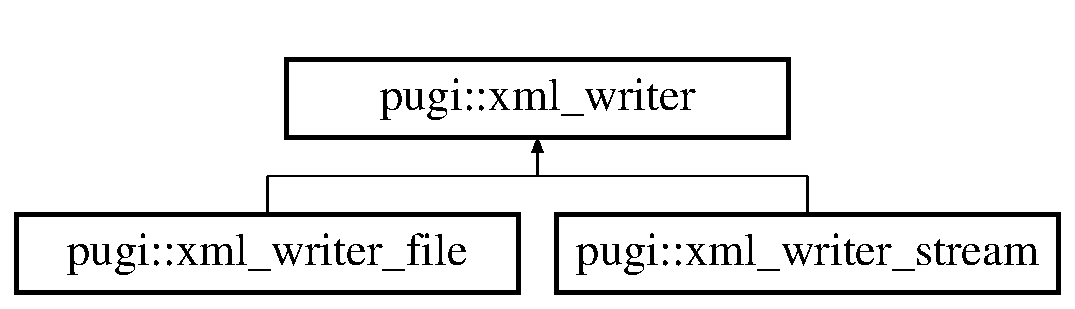
\includegraphics[height=2.000000cm]{classpugi_1_1xml__writer}
\end{center}
\end{figure}
\subsection*{Public Member Functions}
\begin{DoxyCompactItemize}
\item 
virtual \hyperlink{classpugi_1_1xml__writer_a5c9b1bd029ed10862ffa4c61d24c351f}{$\sim$xml\-\_\-writer} ()
\item 
virtual void \hyperlink{classpugi_1_1xml__writer_ab7d3b6a8499ceef7799158370e1c2617}{write} (const void $\ast$data, size\-\_\-t size)=0
\end{DoxyCompactItemize}


\subsection{Constructor \& Destructor Documentation}
\hypertarget{classpugi_1_1xml__writer_a5c9b1bd029ed10862ffa4c61d24c351f}{\index{pugi\-::xml\-\_\-writer@{pugi\-::xml\-\_\-writer}!$\sim$xml\-\_\-writer@{$\sim$xml\-\_\-writer}}
\index{$\sim$xml\-\_\-writer@{$\sim$xml\-\_\-writer}!pugi::xml_writer@{pugi\-::xml\-\_\-writer}}
\subsubsection[{$\sim$xml\-\_\-writer}]{\setlength{\rightskip}{0pt plus 5cm}virtual pugi\-::xml\-\_\-writer\-::$\sim$xml\-\_\-writer (
\begin{DoxyParamCaption}
{}
\end{DoxyParamCaption}
)\hspace{0.3cm}{\ttfamily [inline]}, {\ttfamily [virtual]}}}\label{classpugi_1_1xml__writer_a5c9b1bd029ed10862ffa4c61d24c351f}

\begin{DoxyCode}
236 \{\}
\end{DoxyCode}


\subsection{Member Function Documentation}
\hypertarget{classpugi_1_1xml__writer_ab7d3b6a8499ceef7799158370e1c2617}{\index{pugi\-::xml\-\_\-writer@{pugi\-::xml\-\_\-writer}!write@{write}}
\index{write@{write}!pugi::xml_writer@{pugi\-::xml\-\_\-writer}}
\subsubsection[{write}]{\setlength{\rightskip}{0pt plus 5cm}virtual void pugi\-::xml\-\_\-writer\-::write (
\begin{DoxyParamCaption}
\item[{const void $\ast$}]{data, }
\item[{size\-\_\-t}]{size}
\end{DoxyParamCaption}
)\hspace{0.3cm}{\ttfamily [pure virtual]}}}\label{classpugi_1_1xml__writer_ab7d3b6a8499ceef7799158370e1c2617}


Implemented in \hyperlink{classpugi_1_1xml__writer__stream_a3ec185992d56341f6ee8d1037a6efb17}{pugi\-::xml\-\_\-writer\-\_\-stream}, and \hyperlink{classpugi_1_1xml__writer__file_a228a6e448d8fdbc155032e6eab5d86ed}{pugi\-::xml\-\_\-writer\-\_\-file}.



The documentation for this class was generated from the following file\-:\begin{DoxyCompactItemize}
\item 
Third\-Party/pugixml/\hyperlink{pugixml_8hpp}{pugixml.\-hpp}\end{DoxyCompactItemize}

\hypertarget{classpugi_1_1xml__writer__file}{\section{pugi\-:\-:xml\-\_\-writer\-\_\-file Class Reference}
\label{classpugi_1_1xml__writer__file}\index{pugi\-::xml\-\_\-writer\-\_\-file@{pugi\-::xml\-\_\-writer\-\_\-file}}
}


{\ttfamily \#include $<$pugixml.\-hpp$>$}

Inheritance diagram for pugi\-:\-:xml\-\_\-writer\-\_\-file\-:\begin{figure}[H]
\begin{center}
\leavevmode
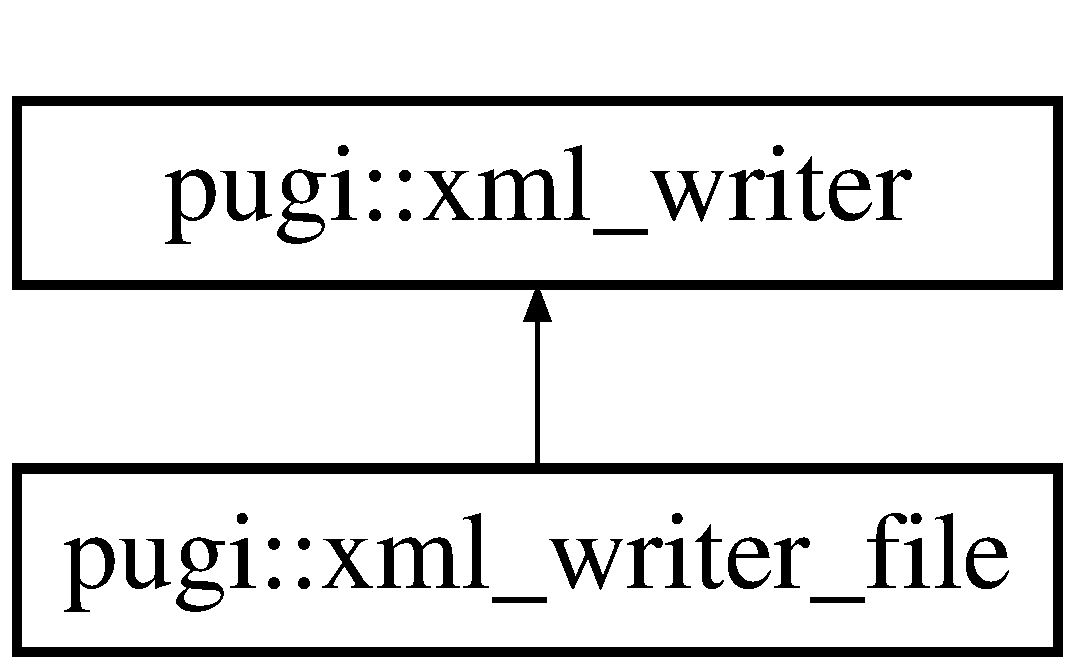
\includegraphics[height=2.000000cm]{classpugi_1_1xml__writer__file}
\end{center}
\end{figure}
\subsection*{Public Member Functions}
\begin{DoxyCompactItemize}
\item 
\hyperlink{classpugi_1_1xml__writer__file_a458afaf5231f88e182fa16b13fc2b0a6}{xml\-\_\-writer\-\_\-file} (void $\ast$file)
\item 
virtual void \hyperlink{classpugi_1_1xml__writer__file_a228a6e448d8fdbc155032e6eab5d86ed}{write} (const void $\ast$data, size\-\_\-t size)
\end{DoxyCompactItemize}


\subsection{Constructor \& Destructor Documentation}
\hypertarget{classpugi_1_1xml__writer__file_a458afaf5231f88e182fa16b13fc2b0a6}{\index{pugi\-::xml\-\_\-writer\-\_\-file@{pugi\-::xml\-\_\-writer\-\_\-file}!xml\-\_\-writer\-\_\-file@{xml\-\_\-writer\-\_\-file}}
\index{xml\-\_\-writer\-\_\-file@{xml\-\_\-writer\-\_\-file}!pugi::xml_writer_file@{pugi\-::xml\-\_\-writer\-\_\-file}}
\subsubsection[{xml\-\_\-writer\-\_\-file}]{\setlength{\rightskip}{0pt plus 5cm}{\bf P\-U\-G\-I\-\_\-\-\_\-\-F\-N} pugi\-::xml\-\_\-writer\-\_\-file\-::xml\-\_\-writer\-\_\-file (
\begin{DoxyParamCaption}
\item[{void $\ast$}]{file}
\end{DoxyParamCaption}
)}}\label{classpugi_1_1xml__writer__file_a458afaf5231f88e182fa16b13fc2b0a6}

\begin{DoxyCode}
3657                                                         : file(file\_)
3658     \{
3659     \}
\end{DoxyCode}


\subsection{Member Function Documentation}
\hypertarget{classpugi_1_1xml__writer__file_a228a6e448d8fdbc155032e6eab5d86ed}{\index{pugi\-::xml\-\_\-writer\-\_\-file@{pugi\-::xml\-\_\-writer\-\_\-file}!write@{write}}
\index{write@{write}!pugi::xml_writer_file@{pugi\-::xml\-\_\-writer\-\_\-file}}
\subsubsection[{write}]{\setlength{\rightskip}{0pt plus 5cm}{\bf P\-U\-G\-I\-\_\-\-\_\-\-F\-N} void pugi\-::xml\-\_\-writer\-\_\-file\-::write (
\begin{DoxyParamCaption}
\item[{const void $\ast$}]{data, }
\item[{size\-\_\-t}]{size}
\end{DoxyParamCaption}
)\hspace{0.3cm}{\ttfamily [virtual]}}}\label{classpugi_1_1xml__writer__file_a228a6e448d8fdbc155032e6eab5d86ed}


Implements \hyperlink{classpugi_1_1xml__writer_ab7d3b6a8499ceef7799158370e1c2617}{pugi\-::xml\-\_\-writer}.


\begin{DoxyCode}
3662     \{
3663         \textcolor{keywordtype}{size\_t} result = fwrite(data, 1, size, static\_cast<FILE*>(file));
3664         (void)!result; \textcolor{comment}{// unfortunately we can't do proper error handling here}
3665     \}
\end{DoxyCode}


The documentation for this class was generated from the following files\-:\begin{DoxyCompactItemize}
\item 
Third\-Party/pugixml/\hyperlink{pugixml_8hpp}{pugixml.\-hpp}\item 
Third\-Party/pugixml/\hyperlink{pugixml_8cpp}{pugixml.\-cpp}\end{DoxyCompactItemize}

\hypertarget{classpugi_1_1xml__writer__stream}{\section{pugi\-:\-:xml\-\_\-writer\-\_\-stream Class Reference}
\label{classpugi_1_1xml__writer__stream}\index{pugi\-::xml\-\_\-writer\-\_\-stream@{pugi\-::xml\-\_\-writer\-\_\-stream}}
}


{\ttfamily \#include $<$pugixml.\-hpp$>$}

Inheritance diagram for pugi\-:\-:xml\-\_\-writer\-\_\-stream\-:\begin{figure}[H]
\begin{center}
\leavevmode
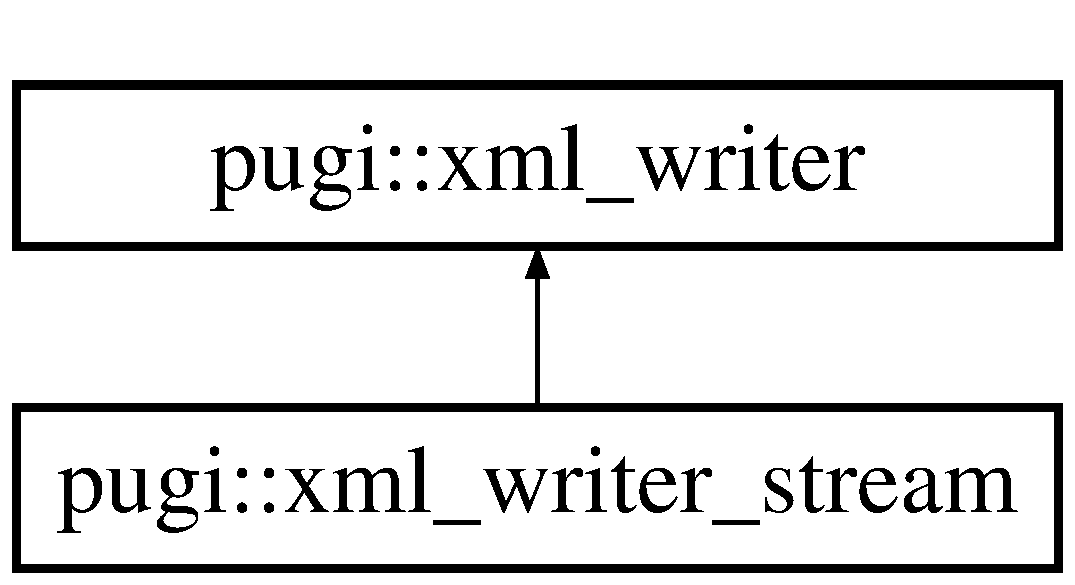
\includegraphics[height=2.000000cm]{classpugi_1_1xml__writer__stream}
\end{center}
\end{figure}
\subsection*{Public Member Functions}
\begin{DoxyCompactItemize}
\item 
\hyperlink{classpugi_1_1xml__writer__stream_a259c28368c08378e15cf28b35a1dcd9a}{xml\-\_\-writer\-\_\-stream} (std\-::basic\-\_\-ostream$<$ char, std\-::char\-\_\-traits$<$ char $>$ $>$ \&stream)
\item 
\hyperlink{classpugi_1_1xml__writer__stream_afa342cf0bb3a0bd6ee3d47550ad23333}{xml\-\_\-writer\-\_\-stream} (std\-::basic\-\_\-ostream$<$ wchar\-\_\-t, std\-::char\-\_\-traits$<$ wchar\-\_\-t $>$ $>$ \&stream)
\item 
virtual void \hyperlink{classpugi_1_1xml__writer__stream_a3ec185992d56341f6ee8d1037a6efb17}{write} (const void $\ast$data, size\-\_\-t size)
\end{DoxyCompactItemize}


\subsection{Constructor \& Destructor Documentation}
\hypertarget{classpugi_1_1xml__writer__stream_a259c28368c08378e15cf28b35a1dcd9a}{\index{pugi\-::xml\-\_\-writer\-\_\-stream@{pugi\-::xml\-\_\-writer\-\_\-stream}!xml\-\_\-writer\-\_\-stream@{xml\-\_\-writer\-\_\-stream}}
\index{xml\-\_\-writer\-\_\-stream@{xml\-\_\-writer\-\_\-stream}!pugi::xml_writer_stream@{pugi\-::xml\-\_\-writer\-\_\-stream}}
\subsubsection[{xml\-\_\-writer\-\_\-stream}]{\setlength{\rightskip}{0pt plus 5cm}{\bf P\-U\-G\-I\-\_\-\-\_\-\-F\-N} pugi\-::xml\-\_\-writer\-\_\-stream\-::xml\-\_\-writer\-\_\-stream (
\begin{DoxyParamCaption}
\item[{std\-::basic\-\_\-ostream$<$ char, std\-::char\-\_\-traits$<$ char $>$ $>$ \&}]{stream}
\end{DoxyParamCaption}
)}}\label{classpugi_1_1xml__writer__stream_a259c28368c08378e15cf28b35a1dcd9a}

\begin{DoxyCode}
3668                                                                                                       : 
      narrow\_stream(&stream), wide\_stream(0)
3669     \{
3670     \}
\end{DoxyCode}
\hypertarget{classpugi_1_1xml__writer__stream_afa342cf0bb3a0bd6ee3d47550ad23333}{\index{pugi\-::xml\-\_\-writer\-\_\-stream@{pugi\-::xml\-\_\-writer\-\_\-stream}!xml\-\_\-writer\-\_\-stream@{xml\-\_\-writer\-\_\-stream}}
\index{xml\-\_\-writer\-\_\-stream@{xml\-\_\-writer\-\_\-stream}!pugi::xml_writer_stream@{pugi\-::xml\-\_\-writer\-\_\-stream}}
\subsubsection[{xml\-\_\-writer\-\_\-stream}]{\setlength{\rightskip}{0pt plus 5cm}{\bf P\-U\-G\-I\-\_\-\-\_\-\-F\-N} pugi\-::xml\-\_\-writer\-\_\-stream\-::xml\-\_\-writer\-\_\-stream (
\begin{DoxyParamCaption}
\item[{std\-::basic\-\_\-ostream$<$ wchar\-\_\-t, std\-::char\-\_\-traits$<$ wchar\-\_\-t $>$ $>$ \&}]{stream}
\end{DoxyParamCaption}
)}}\label{classpugi_1_1xml__writer__stream_afa342cf0bb3a0bd6ee3d47550ad23333}

\begin{DoxyCode}
3672                                                                                                            
       : narrow\_stream(0), wide\_stream(&stream)
3673     \{
3674     \}
\end{DoxyCode}


\subsection{Member Function Documentation}
\hypertarget{classpugi_1_1xml__writer__stream_a3ec185992d56341f6ee8d1037a6efb17}{\index{pugi\-::xml\-\_\-writer\-\_\-stream@{pugi\-::xml\-\_\-writer\-\_\-stream}!write@{write}}
\index{write@{write}!pugi::xml_writer_stream@{pugi\-::xml\-\_\-writer\-\_\-stream}}
\subsubsection[{write}]{\setlength{\rightskip}{0pt plus 5cm}{\bf P\-U\-G\-I\-\_\-\-\_\-\-F\-N} void pugi\-::xml\-\_\-writer\-\_\-stream\-::write (
\begin{DoxyParamCaption}
\item[{const void $\ast$}]{data, }
\item[{size\-\_\-t}]{size}
\end{DoxyParamCaption}
)\hspace{0.3cm}{\ttfamily [virtual]}}}\label{classpugi_1_1xml__writer__stream_a3ec185992d56341f6ee8d1037a6efb17}


Implements \hyperlink{classpugi_1_1xml__writer_ab7d3b6a8499ceef7799158370e1c2617}{pugi\-::xml\-\_\-writer}.


\begin{DoxyCode}
3677     \{
3678         \textcolor{keywordflow}{if} (narrow\_stream)
3679         \{
3680             assert(!wide\_stream);
3681             narrow\_stream->write(reinterpret\_cast<const char*>(data), static\_cast<std::streamsize>(size));
3682         \}
3683         \textcolor{keywordflow}{else}
3684         \{
3685             assert(wide\_stream);
3686             assert(size % \textcolor{keyword}{sizeof}(\textcolor{keywordtype}{wchar\_t}) == 0);
3687 
3688             wide\_stream->write(reinterpret\_cast<const wchar\_t*>(data), static\_cast<std::streamsize>(size / \textcolor{keyword}{
      sizeof}(\textcolor{keywordtype}{wchar\_t})));
3689         \}
3690     \}
\end{DoxyCode}


The documentation for this class was generated from the following files\-:\begin{DoxyCompactItemize}
\item 
Third\-Party/pugixml/\hyperlink{pugixml_8hpp}{pugixml.\-hpp}\item 
Third\-Party/pugixml/\hyperlink{pugixml_8cpp}{pugixml.\-cpp}\end{DoxyCompactItemize}

\hypertarget{classxpath__allocator}{\section{xpath\-\_\-allocator Class Reference}
\label{classxpath__allocator}\index{xpath\-\_\-allocator@{xpath\-\_\-allocator}}
}
\subsection*{Public Member Functions}
\begin{DoxyCompactItemize}
\item 
\hyperlink{classxpath__allocator_a3b8ba1722fba115d05949d8f592080e8}{xpath\-\_\-allocator} (\hyperlink{structxpath__memory__block}{xpath\-\_\-memory\-\_\-block} $\ast$root, size\-\_\-t root\-\_\-size=0)
\item 
void $\ast$ \hyperlink{classxpath__allocator_aa66f3703548657eca5316392a2d79d00}{allocate\-\_\-nothrow} (size\-\_\-t size)
\item 
void $\ast$ \hyperlink{classxpath__allocator_aad95aa445f2fdc7c3d1c19b1f3d67cb1}{allocate} (size\-\_\-t size)
\item 
void $\ast$ \hyperlink{classxpath__allocator_a4dd502389202ec8e7420832112a571e5}{reallocate} (void $\ast$ptr, size\-\_\-t old\-\_\-size, size\-\_\-t new\-\_\-size)
\item 
void \hyperlink{classxpath__allocator_af1c3ec117935d4488bbd16adf807fbc1}{revert} (const \hyperlink{classxpath__allocator}{xpath\-\_\-allocator} \&state)
\item 
void \hyperlink{classxpath__allocator_a9436b8bdef3e0e0ff0df28c2af6a430d}{release} ()
\end{DoxyCompactItemize}


\subsection{Constructor \& Destructor Documentation}
\hypertarget{classxpath__allocator_a3b8ba1722fba115d05949d8f592080e8}{\index{xpath\-\_\-allocator@{xpath\-\_\-allocator}!xpath\-\_\-allocator@{xpath\-\_\-allocator}}
\index{xpath\-\_\-allocator@{xpath\-\_\-allocator}!xpath_allocator@{xpath\-\_\-allocator}}
\subsubsection[{xpath\-\_\-allocator}]{\setlength{\rightskip}{0pt plus 5cm}xpath\-\_\-allocator\-::xpath\-\_\-allocator (
\begin{DoxyParamCaption}
\item[{{\bf xpath\-\_\-memory\-\_\-block} $\ast$}]{root, }
\item[{size\-\_\-t}]{root\-\_\-size = {\ttfamily 0}}
\end{DoxyParamCaption}
)\hspace{0.3cm}{\ttfamily [inline]}}}\label{classxpath__allocator_a3b8ba1722fba115d05949d8f592080e8}

\begin{DoxyCode}
5675                                                                        : \_root(root), \_root\_size(root\_size)
5676         \{
5677 \textcolor{preprocessor}{        #ifdef PUGIXML\_NO\_EXCEPTIONS}
5678 \textcolor{preprocessor}{}            error\_handler = 0;
5679 \textcolor{preprocessor}{        #endif}
5680 \textcolor{preprocessor}{}        \}
\end{DoxyCode}


\subsection{Member Function Documentation}
\hypertarget{classxpath__allocator_aad95aa445f2fdc7c3d1c19b1f3d67cb1}{\index{xpath\-\_\-allocator@{xpath\-\_\-allocator}!allocate@{allocate}}
\index{allocate@{allocate}!xpath_allocator@{xpath\-\_\-allocator}}
\subsubsection[{allocate}]{\setlength{\rightskip}{0pt plus 5cm}void$\ast$ xpath\-\_\-allocator\-::allocate (
\begin{DoxyParamCaption}
\item[{size\-\_\-t}]{size}
\end{DoxyParamCaption}
)\hspace{0.3cm}{\ttfamily [inline]}}}\label{classxpath__allocator_aad95aa445f2fdc7c3d1c19b1f3d67cb1}

\begin{DoxyCode}
5713         \{
5714             \textcolor{keywordtype}{void}* result = \hyperlink{classxpath__allocator_aa66f3703548657eca5316392a2d79d00}{allocate\_nothrow}(size);
5715 
5716             \textcolor{keywordflow}{if} (!result)
5717             \{
5718 \textcolor{preprocessor}{            #ifdef PUGIXML\_NO\_EXCEPTIONS}
5719 \textcolor{preprocessor}{}                assert(error\_handler);
5720                 longjmp(*error\_handler, 1);
5721 \textcolor{preprocessor}{            #else}
5722 \textcolor{preprocessor}{}                \textcolor{keywordflow}{throw} std::bad\_alloc();
5723 \textcolor{preprocessor}{            #endif}
5724 \textcolor{preprocessor}{}            \}
5725 
5726             \textcolor{keywordflow}{return} result;
5727         \}
\end{DoxyCode}
\hypertarget{classxpath__allocator_aa66f3703548657eca5316392a2d79d00}{\index{xpath\-\_\-allocator@{xpath\-\_\-allocator}!allocate\-\_\-nothrow@{allocate\-\_\-nothrow}}
\index{allocate\-\_\-nothrow@{allocate\-\_\-nothrow}!xpath_allocator@{xpath\-\_\-allocator}}
\subsubsection[{allocate\-\_\-nothrow}]{\setlength{\rightskip}{0pt plus 5cm}void$\ast$ xpath\-\_\-allocator\-::allocate\-\_\-nothrow (
\begin{DoxyParamCaption}
\item[{size\-\_\-t}]{size}
\end{DoxyParamCaption}
)\hspace{0.3cm}{\ttfamily [inline]}}}\label{classxpath__allocator_aa66f3703548657eca5316392a2d79d00}

\begin{DoxyCode}
5683         \{
5684             \textcolor{keyword}{const} \textcolor{keywordtype}{size\_t} block\_capacity = \textcolor{keyword}{sizeof}(\_root->\hyperlink{structxpath__memory__block_a7b00376d0eac172ab537b6b0964858a9}{data});
5685 
5686             \textcolor{comment}{// align size so that we're able to store pointers in subsequent blocks}
5687             size = (size + \textcolor{keyword}{sizeof}(\textcolor{keywordtype}{void}*) - 1) & ~(\textcolor{keyword}{sizeof}(\textcolor{keywordtype}{void}*) - 1);
5688 
5689             \textcolor{keywordflow}{if} (\_root\_size + size <= block\_capacity)
5690             \{
5691                 \textcolor{keywordtype}{void}* buf = \_root->\hyperlink{structxpath__memory__block_a7b00376d0eac172ab537b6b0964858a9}{data} + \_root\_size;
5692                 \_root\_size += size;
5693                 \textcolor{keywordflow}{return} buf;
5694             \}
5695             \textcolor{keywordflow}{else}
5696             \{
5697                 \textcolor{keywordtype}{size\_t} block\_data\_size = (size > block\_capacity) ? size : block\_capacity;
5698                 \textcolor{keywordtype}{size\_t} block\_size = block\_data\_size + offsetof(
      \hyperlink{structxpath__memory__block}{xpath\_memory\_block}, data);
5699 
5700                 \hyperlink{structxpath__memory__block}{xpath\_memory\_block}* block = \textcolor{keyword}{static\_cast<}
      \hyperlink{structxpath__memory__block}{xpath\_memory\_block}*\textcolor{keyword}{>}(\hyperlink{structxml__memory__management__function__storage_abb6865f8d07d27fd9273737c59f6e941}{xml\_memory::allocate}(block\_size));
5701                 \textcolor{keywordflow}{if} (!block) \textcolor{keywordflow}{return} 0;
5702                 
5703                 block->\hyperlink{structxpath__memory__block_ab7f0d8400b40a51cdb063e76fd19a93c}{next} = \_root;
5704                 
5705                 \_root = block;
5706                 \_root\_size = size;
5707                 
5708                 \textcolor{keywordflow}{return} block->\hyperlink{structxpath__memory__block_a7b00376d0eac172ab537b6b0964858a9}{data};
5709             \}
5710         \}
\end{DoxyCode}
\hypertarget{classxpath__allocator_a4dd502389202ec8e7420832112a571e5}{\index{xpath\-\_\-allocator@{xpath\-\_\-allocator}!reallocate@{reallocate}}
\index{reallocate@{reallocate}!xpath_allocator@{xpath\-\_\-allocator}}
\subsubsection[{reallocate}]{\setlength{\rightskip}{0pt plus 5cm}void$\ast$ xpath\-\_\-allocator\-::reallocate (
\begin{DoxyParamCaption}
\item[{void $\ast$}]{ptr, }
\item[{size\-\_\-t}]{old\-\_\-size, }
\item[{size\-\_\-t}]{new\-\_\-size}
\end{DoxyParamCaption}
)\hspace{0.3cm}{\ttfamily [inline]}}}\label{classxpath__allocator_a4dd502389202ec8e7420832112a571e5}

\begin{DoxyCode}
5730         \{
5731             \textcolor{comment}{// align size so that we're able to store pointers in subsequent blocks}
5732             old\_size = (old\_size + \textcolor{keyword}{sizeof}(\textcolor{keywordtype}{void}*) - 1) & ~(\textcolor{keyword}{sizeof}(\textcolor{keywordtype}{void}*) - 1);
5733             new\_size = (new\_size + \textcolor{keyword}{sizeof}(\textcolor{keywordtype}{void}*) - 1) & ~(\textcolor{keyword}{sizeof}(\textcolor{keywordtype}{void}*) - 1);
5734 
5735             \textcolor{comment}{// we can only reallocate the last object}
5736             assert(ptr == 0 || static\_cast<char*>(ptr) + old\_size == \_root->\hyperlink{structxpath__memory__block_a7b00376d0eac172ab537b6b0964858a9}{data} + \_root\_size);
5737 
5738             \textcolor{comment}{// adjust root size so that we have not allocated the object at all}
5739             \textcolor{keywordtype}{bool} only\_object = (\_root\_size == old\_size);
5740 
5741             \textcolor{keywordflow}{if} (ptr) \_root\_size -= old\_size;
5742 
5743             \textcolor{comment}{// allocate a new version (this will obviously reuse the memory if possible)}
5744             \textcolor{keywordtype}{void}* result = \hyperlink{classxpath__allocator_aad95aa445f2fdc7c3d1c19b1f3d67cb1}{allocate}(new\_size);
5745             assert(result);
5746 
5747             \textcolor{comment}{// we have a new block}
5748             \textcolor{keywordflow}{if} (result != ptr && ptr)
5749             \{
5750                 \textcolor{comment}{// copy old data}
5751                 assert(new\_size > old\_size);
5752                 memcpy(result, ptr, old\_size);
5753 
5754                 \textcolor{comment}{// free the previous page if it had no other objects}
5755                 \textcolor{keywordflow}{if} (only\_object)
5756                 \{
5757                     assert(\_root->\hyperlink{structxpath__memory__block_a7b00376d0eac172ab537b6b0964858a9}{data} == result);
5758                     assert(\_root->\hyperlink{structxpath__memory__block_ab7f0d8400b40a51cdb063e76fd19a93c}{next});
5759 
5760                     \hyperlink{structxpath__memory__block}{xpath\_memory\_block}* next = \_root->\hyperlink{structxpath__memory__block_ab7f0d8400b40a51cdb063e76fd19a93c}{next}->
      \hyperlink{structxpath__memory__block_ab7f0d8400b40a51cdb063e76fd19a93c}{next};
5761 
5762                     \textcolor{keywordflow}{if} (next)
5763                     \{
5764                         \textcolor{comment}{// deallocate the whole page, unless it was the first one}
5765                         \hyperlink{structxml__memory__management__function__storage_a1c80a9a045ed6cfb90b17a178e4b3512}{xml\_memory::deallocate}(\_root->\hyperlink{structxpath__memory__block_ab7f0d8400b40a51cdb063e76fd19a93c}{next});
5766                         \_root->\hyperlink{structxpath__memory__block_ab7f0d8400b40a51cdb063e76fd19a93c}{next} = next;
5767                     \}
5768                 \}
5769             \}
5770 
5771             \textcolor{keywordflow}{return} result;
5772         \}
\end{DoxyCode}
\hypertarget{classxpath__allocator_a9436b8bdef3e0e0ff0df28c2af6a430d}{\index{xpath\-\_\-allocator@{xpath\-\_\-allocator}!release@{release}}
\index{release@{release}!xpath_allocator@{xpath\-\_\-allocator}}
\subsubsection[{release}]{\setlength{\rightskip}{0pt plus 5cm}void xpath\-\_\-allocator\-::release (
\begin{DoxyParamCaption}
{}
\end{DoxyParamCaption}
)\hspace{0.3cm}{\ttfamily [inline]}}}\label{classxpath__allocator_a9436b8bdef3e0e0ff0df28c2af6a430d}

\begin{DoxyCode}
5794         \{
5795             \hyperlink{structxpath__memory__block}{xpath\_memory\_block}* cur = \_root;
5796             assert(cur);
5797 
5798             \textcolor{keywordflow}{while} (cur->\hyperlink{structxpath__memory__block_ab7f0d8400b40a51cdb063e76fd19a93c}{next})
5799             \{
5800                 \hyperlink{structxpath__memory__block}{xpath\_memory\_block}* next = cur->\hyperlink{structxpath__memory__block_ab7f0d8400b40a51cdb063e76fd19a93c}{next};
5801 
5802                 \hyperlink{structxml__memory__management__function__storage_a1c80a9a045ed6cfb90b17a178e4b3512}{xml\_memory::deallocate}(cur);
5803 
5804                 cur = next;
5805             \}
5806         \}
\end{DoxyCode}
\hypertarget{classxpath__allocator_af1c3ec117935d4488bbd16adf807fbc1}{\index{xpath\-\_\-allocator@{xpath\-\_\-allocator}!revert@{revert}}
\index{revert@{revert}!xpath_allocator@{xpath\-\_\-allocator}}
\subsubsection[{revert}]{\setlength{\rightskip}{0pt plus 5cm}void xpath\-\_\-allocator\-::revert (
\begin{DoxyParamCaption}
\item[{const {\bf xpath\-\_\-allocator} \&}]{state}
\end{DoxyParamCaption}
)\hspace{0.3cm}{\ttfamily [inline]}}}\label{classxpath__allocator_af1c3ec117935d4488bbd16adf807fbc1}

\begin{DoxyCode}
5775         \{
5776             \textcolor{comment}{// free all new pages}
5777             \hyperlink{structxpath__memory__block}{xpath\_memory\_block}* cur = \_root;
5778 
5779             \textcolor{keywordflow}{while} (cur != state.\_root)
5780             \{
5781                 \hyperlink{structxpath__memory__block}{xpath\_memory\_block}* next = cur->\hyperlink{structxpath__memory__block_ab7f0d8400b40a51cdb063e76fd19a93c}{next};
5782 
5783                 \hyperlink{structxml__memory__management__function__storage_a1c80a9a045ed6cfb90b17a178e4b3512}{xml\_memory::deallocate}(cur);
5784 
5785                 cur = next;
5786             \}
5787 
5788             \textcolor{comment}{// restore state}
5789             \_root = state.\_root;
5790             \_root\_size = state.\_root\_size;
5791         \}
\end{DoxyCode}


The documentation for this class was generated from the following file\-:\begin{DoxyCompactItemize}
\item 
Third\-Party/pugixml/\hyperlink{pugixml_8cpp}{pugixml.\-cpp}\end{DoxyCompactItemize}

\hypertarget{structxpath__allocator__capture}{\section{xpath\-\_\-allocator\-\_\-capture Struct Reference}
\label{structxpath__allocator__capture}\index{xpath\-\_\-allocator\-\_\-capture@{xpath\-\_\-allocator\-\_\-capture}}
}
\subsection*{Public Member Functions}
\begin{DoxyCompactItemize}
\item 
\hyperlink{structxpath__allocator__capture_af6925e08c811c0cbda74d4da5b9f2eed}{xpath\-\_\-allocator\-\_\-capture} (\hyperlink{classxpath__allocator}{xpath\-\_\-allocator} $\ast$alloc)
\item 
\hyperlink{structxpath__allocator__capture_a09d4f62de6a543483b94eec405667101}{$\sim$xpath\-\_\-allocator\-\_\-capture} ()
\end{DoxyCompactItemize}
\subsection*{Data Fields}
\begin{DoxyCompactItemize}
\item 
\hyperlink{classxpath__allocator}{xpath\-\_\-allocator} $\ast$ \hyperlink{structxpath__allocator__capture_a382acca931c691699ec84a03fb060cf4}{\-\_\-target}
\item 
\hyperlink{classxpath__allocator}{xpath\-\_\-allocator} \hyperlink{structxpath__allocator__capture_a275859dc99681c12b42ee4f51b713d39}{\-\_\-state}
\end{DoxyCompactItemize}


\subsection{Constructor \& Destructor Documentation}
\hypertarget{structxpath__allocator__capture_af6925e08c811c0cbda74d4da5b9f2eed}{\index{xpath\-\_\-allocator\-\_\-capture@{xpath\-\_\-allocator\-\_\-capture}!xpath\-\_\-allocator\-\_\-capture@{xpath\-\_\-allocator\-\_\-capture}}
\index{xpath\-\_\-allocator\-\_\-capture@{xpath\-\_\-allocator\-\_\-capture}!xpath_allocator_capture@{xpath\-\_\-allocator\-\_\-capture}}
\subsubsection[{xpath\-\_\-allocator\-\_\-capture}]{\setlength{\rightskip}{0pt plus 5cm}xpath\-\_\-allocator\-\_\-capture\-::xpath\-\_\-allocator\-\_\-capture (
\begin{DoxyParamCaption}
\item[{{\bf xpath\-\_\-allocator} $\ast$}]{alloc}
\end{DoxyParamCaption}
)\hspace{0.3cm}{\ttfamily [inline]}}}\label{structxpath__allocator__capture_af6925e08c811c0cbda74d4da5b9f2eed}

\begin{DoxyCode}
5811                                                        : \hyperlink{structxpath__allocator__capture_a382acca931c691699ec84a03fb060cf4}{\_target}(alloc), 
      \hyperlink{structxpath__allocator__capture_a275859dc99681c12b42ee4f51b713d39}{\_state}(*alloc)
5812         \{
5813         \}
\end{DoxyCode}
\hypertarget{structxpath__allocator__capture_a09d4f62de6a543483b94eec405667101}{\index{xpath\-\_\-allocator\-\_\-capture@{xpath\-\_\-allocator\-\_\-capture}!$\sim$xpath\-\_\-allocator\-\_\-capture@{$\sim$xpath\-\_\-allocator\-\_\-capture}}
\index{$\sim$xpath\-\_\-allocator\-\_\-capture@{$\sim$xpath\-\_\-allocator\-\_\-capture}!xpath_allocator_capture@{xpath\-\_\-allocator\-\_\-capture}}
\subsubsection[{$\sim$xpath\-\_\-allocator\-\_\-capture}]{\setlength{\rightskip}{0pt plus 5cm}xpath\-\_\-allocator\-\_\-capture\-::$\sim$xpath\-\_\-allocator\-\_\-capture (
\begin{DoxyParamCaption}
{}
\end{DoxyParamCaption}
)\hspace{0.3cm}{\ttfamily [inline]}}}\label{structxpath__allocator__capture_a09d4f62de6a543483b94eec405667101}

\begin{DoxyCode}
5816         \{
5817             \hyperlink{structxpath__allocator__capture_a382acca931c691699ec84a03fb060cf4}{\_target}->\hyperlink{classxpath__allocator_af1c3ec117935d4488bbd16adf807fbc1}{revert}(\hyperlink{structxpath__allocator__capture_a275859dc99681c12b42ee4f51b713d39}{\_state});
5818         \}
\end{DoxyCode}


\subsection{Field Documentation}
\hypertarget{structxpath__allocator__capture_a275859dc99681c12b42ee4f51b713d39}{\index{xpath\-\_\-allocator\-\_\-capture@{xpath\-\_\-allocator\-\_\-capture}!\-\_\-state@{\-\_\-state}}
\index{\-\_\-state@{\-\_\-state}!xpath_allocator_capture@{xpath\-\_\-allocator\-\_\-capture}}
\subsubsection[{\-\_\-state}]{\setlength{\rightskip}{0pt plus 5cm}{\bf xpath\-\_\-allocator} xpath\-\_\-allocator\-\_\-capture\-::\-\_\-state}}\label{structxpath__allocator__capture_a275859dc99681c12b42ee4f51b713d39}
\hypertarget{structxpath__allocator__capture_a382acca931c691699ec84a03fb060cf4}{\index{xpath\-\_\-allocator\-\_\-capture@{xpath\-\_\-allocator\-\_\-capture}!\-\_\-target@{\-\_\-target}}
\index{\-\_\-target@{\-\_\-target}!xpath_allocator_capture@{xpath\-\_\-allocator\-\_\-capture}}
\subsubsection[{\-\_\-target}]{\setlength{\rightskip}{0pt plus 5cm}{\bf xpath\-\_\-allocator}$\ast$ xpath\-\_\-allocator\-\_\-capture\-::\-\_\-target}}\label{structxpath__allocator__capture_a382acca931c691699ec84a03fb060cf4}


The documentation for this struct was generated from the following file\-:\begin{DoxyCompactItemize}
\item 
Third\-Party/pugixml/\hyperlink{pugixml_8cpp}{pugixml.\-cpp}\end{DoxyCompactItemize}

\hypertarget{classxpath__ast__node}{\section{xpath\-\_\-ast\-\_\-node Class Reference}
\label{classxpath__ast__node}\index{xpath\-\_\-ast\-\_\-node@{xpath\-\_\-ast\-\_\-node}}
}
\subsection*{Public Member Functions}
\begin{DoxyCompactItemize}
\item 
\hyperlink{classxpath__ast__node_af155d17a4477a693d37f4e34957dcc21}{xpath\-\_\-ast\-\_\-node} (\hyperlink{pugixml_8cpp_a11258a240266b84b6b0526930e5d330d}{ast\-\_\-type\-\_\-t} type, xpath\-\_\-value\-\_\-type rettype\-\_\-, const char\-\_\-t $\ast$value)
\item 
\hyperlink{classxpath__ast__node_ada97458f3fc7d6c87cf70d8084117b0d}{xpath\-\_\-ast\-\_\-node} (\hyperlink{pugixml_8cpp_a11258a240266b84b6b0526930e5d330d}{ast\-\_\-type\-\_\-t} type, xpath\-\_\-value\-\_\-type rettype\-\_\-, double value)
\item 
\hyperlink{classxpath__ast__node_a8de4244f7b9fc7626049197ddc0afab7}{xpath\-\_\-ast\-\_\-node} (\hyperlink{pugixml_8cpp_a11258a240266b84b6b0526930e5d330d}{ast\-\_\-type\-\_\-t} type, xpath\-\_\-value\-\_\-type rettype\-\_\-, xpath\-\_\-variable $\ast$value)
\item 
\hyperlink{classxpath__ast__node_af6f4ffea3f3c7fdb6ef1e759d4b070f4}{xpath\-\_\-ast\-\_\-node} (\hyperlink{pugixml_8cpp_a11258a240266b84b6b0526930e5d330d}{ast\-\_\-type\-\_\-t} type, xpath\-\_\-value\-\_\-type rettype\-\_\-, \hyperlink{classxpath__ast__node}{xpath\-\_\-ast\-\_\-node} $\ast$left=0, \hyperlink{classxpath__ast__node}{xpath\-\_\-ast\-\_\-node} $\ast$right=0)
\item 
\hyperlink{classxpath__ast__node_a7cf74b277deba86a6575796c727fe458}{xpath\-\_\-ast\-\_\-node} (\hyperlink{pugixml_8cpp_a11258a240266b84b6b0526930e5d330d}{ast\-\_\-type\-\_\-t} type, \hyperlink{classxpath__ast__node}{xpath\-\_\-ast\-\_\-node} $\ast$left, \hyperlink{pugixml_8cpp_ae7747145441b0591a5c04f20f6f9189a}{axis\-\_\-t} axis, \hyperlink{pugixml_8cpp_ab268b4264276130baeb17ab629015275}{nodetest\-\_\-t} test, const char\-\_\-t $\ast$contents)
\item 
void \hyperlink{classxpath__ast__node_a2764184d076834284eb3ff3182b845cc}{set\-\_\-next} (\hyperlink{classxpath__ast__node}{xpath\-\_\-ast\-\_\-node} $\ast$value)
\item 
void \hyperlink{classxpath__ast__node_afe044146db852b7d4dbf188fd2ff6c75}{set\-\_\-right} (\hyperlink{classxpath__ast__node}{xpath\-\_\-ast\-\_\-node} $\ast$value)
\item 
bool \hyperlink{classxpath__ast__node_ab7f965a92023bc2704b8e6fd9f3d7c14}{eval\-\_\-boolean} (const \hyperlink{structxpath__context}{xpath\-\_\-context} \&c, const \hyperlink{structxpath__stack}{xpath\-\_\-stack} \&stack)
\item 
double \hyperlink{classxpath__ast__node_a92dd7048e28d486bc7f382d1fc6f1de6}{eval\-\_\-number} (const \hyperlink{structxpath__context}{xpath\-\_\-context} \&c, const \hyperlink{structxpath__stack}{xpath\-\_\-stack} \&stack)
\item 
\hyperlink{classxpath__string}{xpath\-\_\-string} \hyperlink{classxpath__ast__node_aaf931a091af0fb91c25e90b205363b4e}{eval\-\_\-string\-\_\-concat} (const \hyperlink{structxpath__context}{xpath\-\_\-context} \&c, const \hyperlink{structxpath__stack}{xpath\-\_\-stack} \&stack)
\item 
\hyperlink{classxpath__string}{xpath\-\_\-string} \hyperlink{classxpath__ast__node_a6b675237a590548b68d0e0b97518b6df}{eval\-\_\-string} (const \hyperlink{structxpath__context}{xpath\-\_\-context} \&c, const \hyperlink{structxpath__stack}{xpath\-\_\-stack} \&stack)
\item 
\hyperlink{classxpath__node__set__raw}{xpath\-\_\-node\-\_\-set\-\_\-raw} \hyperlink{classxpath__ast__node_a30d98ec97e3129e82ac9ec3f2a759855}{eval\-\_\-node\-\_\-set} (const \hyperlink{structxpath__context}{xpath\-\_\-context} \&c, const \hyperlink{structxpath__stack}{xpath\-\_\-stack} \&stack)
\item 
bool \hyperlink{classxpath__ast__node_a9253f88832441a357ea65639c73a34be}{is\-\_\-posinv} ()
\item 
xpath\-\_\-value\-\_\-type \hyperlink{classxpath__ast__node_a2c3598521141ed4b763fe6c4f852234f}{rettype} () const 
\end{DoxyCompactItemize}


\subsection{Constructor \& Destructor Documentation}
\hypertarget{classxpath__ast__node_af155d17a4477a693d37f4e34957dcc21}{\index{xpath\-\_\-ast\-\_\-node@{xpath\-\_\-ast\-\_\-node}!xpath\-\_\-ast\-\_\-node@{xpath\-\_\-ast\-\_\-node}}
\index{xpath\-\_\-ast\-\_\-node@{xpath\-\_\-ast\-\_\-node}!xpath_ast_node@{xpath\-\_\-ast\-\_\-node}}
\subsubsection[{xpath\-\_\-ast\-\_\-node}]{\setlength{\rightskip}{0pt plus 5cm}xpath\-\_\-ast\-\_\-node\-::xpath\-\_\-ast\-\_\-node (
\begin{DoxyParamCaption}
\item[{{\bf ast\-\_\-type\-\_\-t}}]{type, }
\item[{xpath\-\_\-value\-\_\-type}]{rettype\-\_\-, }
\item[{const char\-\_\-t $\ast$}]{value}
\end{DoxyParamCaption}
)\hspace{0.3cm}{\ttfamily [inline]}}}\label{classxpath__ast__node_af155d17a4477a693d37f4e34957dcc21}

\begin{DoxyCode}
7979                                                                                        :
7980             \_type(static\_cast<char>(type)), \_rettype(static\_cast<char>(rettype\_)), \_axis(0), \_test(0), 
      \_left(0), \_right(0), \_next(0)
7981         \{
7982             assert(type == \hyperlink{pugixml_8cpp_a11258a240266b84b6b0526930e5d330da9062d53478f8a445ed281f1af75b9ab0}{ast\_string\_constant});
7983             \_data.string = value;
7984         \}
\end{DoxyCode}
\hypertarget{classxpath__ast__node_ada97458f3fc7d6c87cf70d8084117b0d}{\index{xpath\-\_\-ast\-\_\-node@{xpath\-\_\-ast\-\_\-node}!xpath\-\_\-ast\-\_\-node@{xpath\-\_\-ast\-\_\-node}}
\index{xpath\-\_\-ast\-\_\-node@{xpath\-\_\-ast\-\_\-node}!xpath_ast_node@{xpath\-\_\-ast\-\_\-node}}
\subsubsection[{xpath\-\_\-ast\-\_\-node}]{\setlength{\rightskip}{0pt plus 5cm}xpath\-\_\-ast\-\_\-node\-::xpath\-\_\-ast\-\_\-node (
\begin{DoxyParamCaption}
\item[{{\bf ast\-\_\-type\-\_\-t}}]{type, }
\item[{xpath\-\_\-value\-\_\-type}]{rettype\-\_\-, }
\item[{double}]{value}
\end{DoxyParamCaption}
)\hspace{0.3cm}{\ttfamily [inline]}}}\label{classxpath__ast__node_ada97458f3fc7d6c87cf70d8084117b0d}

\begin{DoxyCode}
7986                                                                                 :
7987             \_type(static\_cast<char>(type)), \_rettype(static\_cast<char>(rettype\_)), \_axis(0), \_test(0), 
      \_left(0), \_right(0), \_next(0)
7988         \{
7989             assert(type == \hyperlink{pugixml_8cpp_a11258a240266b84b6b0526930e5d330da09494df03f6c34c5431cb9851a1259ba}{ast\_number\_constant});
7990             \_data.number = value;
7991         \}
\end{DoxyCode}
\hypertarget{classxpath__ast__node_a8de4244f7b9fc7626049197ddc0afab7}{\index{xpath\-\_\-ast\-\_\-node@{xpath\-\_\-ast\-\_\-node}!xpath\-\_\-ast\-\_\-node@{xpath\-\_\-ast\-\_\-node}}
\index{xpath\-\_\-ast\-\_\-node@{xpath\-\_\-ast\-\_\-node}!xpath_ast_node@{xpath\-\_\-ast\-\_\-node}}
\subsubsection[{xpath\-\_\-ast\-\_\-node}]{\setlength{\rightskip}{0pt plus 5cm}xpath\-\_\-ast\-\_\-node\-::xpath\-\_\-ast\-\_\-node (
\begin{DoxyParamCaption}
\item[{{\bf ast\-\_\-type\-\_\-t}}]{type, }
\item[{xpath\-\_\-value\-\_\-type}]{rettype\-\_\-, }
\item[{xpath\-\_\-variable $\ast$}]{value}
\end{DoxyParamCaption}
)\hspace{0.3cm}{\ttfamily [inline]}}}\label{classxpath__ast__node_a8de4244f7b9fc7626049197ddc0afab7}

\begin{DoxyCode}
7993                                                                                          :
7994             \_type(static\_cast<char>(type)), \_rettype(static\_cast<char>(rettype\_)), \_axis(0), \_test(0), 
      \_left(0), \_right(0), \_next(0)
7995         \{
7996             assert(type == \hyperlink{pugixml_8cpp_a11258a240266b84b6b0526930e5d330da3e16540ee352944686b90794e0c94260}{ast\_variable});
7997             \_data.variable = value;
7998         \}
\end{DoxyCode}
\hypertarget{classxpath__ast__node_af6f4ffea3f3c7fdb6ef1e759d4b070f4}{\index{xpath\-\_\-ast\-\_\-node@{xpath\-\_\-ast\-\_\-node}!xpath\-\_\-ast\-\_\-node@{xpath\-\_\-ast\-\_\-node}}
\index{xpath\-\_\-ast\-\_\-node@{xpath\-\_\-ast\-\_\-node}!xpath_ast_node@{xpath\-\_\-ast\-\_\-node}}
\subsubsection[{xpath\-\_\-ast\-\_\-node}]{\setlength{\rightskip}{0pt plus 5cm}xpath\-\_\-ast\-\_\-node\-::xpath\-\_\-ast\-\_\-node (
\begin{DoxyParamCaption}
\item[{{\bf ast\-\_\-type\-\_\-t}}]{type, }
\item[{xpath\-\_\-value\-\_\-type}]{rettype\-\_\-, }
\item[{{\bf xpath\-\_\-ast\-\_\-node} $\ast$}]{left = {\ttfamily 0}, }
\item[{{\bf xpath\-\_\-ast\-\_\-node} $\ast$}]{right = {\ttfamily 0}}
\end{DoxyParamCaption}
)\hspace{0.3cm}{\ttfamily [inline]}}}\label{classxpath__ast__node_af6f4ffea3f3c7fdb6ef1e759d4b070f4}

\begin{DoxyCode}
8000                                                                                                            
                  :
8001             \_type(static\_cast<char>(type)), \_rettype(static\_cast<char>(rettype\_)), \_axis(0), \_test(0), 
      \_left(left), \_right(right), \_next(0)
8002         \{
8003         \}
\end{DoxyCode}
\hypertarget{classxpath__ast__node_a7cf74b277deba86a6575796c727fe458}{\index{xpath\-\_\-ast\-\_\-node@{xpath\-\_\-ast\-\_\-node}!xpath\-\_\-ast\-\_\-node@{xpath\-\_\-ast\-\_\-node}}
\index{xpath\-\_\-ast\-\_\-node@{xpath\-\_\-ast\-\_\-node}!xpath_ast_node@{xpath\-\_\-ast\-\_\-node}}
\subsubsection[{xpath\-\_\-ast\-\_\-node}]{\setlength{\rightskip}{0pt plus 5cm}xpath\-\_\-ast\-\_\-node\-::xpath\-\_\-ast\-\_\-node (
\begin{DoxyParamCaption}
\item[{{\bf ast\-\_\-type\-\_\-t}}]{type, }
\item[{{\bf xpath\-\_\-ast\-\_\-node} $\ast$}]{left, }
\item[{{\bf axis\-\_\-t}}]{axis, }
\item[{{\bf nodetest\-\_\-t}}]{test, }
\item[{const char\-\_\-t $\ast$}]{contents}
\end{DoxyParamCaption}
)\hspace{0.3cm}{\ttfamily [inline]}}}\label{classxpath__ast__node_a7cf74b277deba86a6575796c727fe458}

\begin{DoxyCode}
8005                                                                                                            
              :
8006             \_type(static\_cast<char>(type)), \_rettype(\hyperlink{namespacepugi_ae3820874caf240e9f311bfd2790a84d6af5613748204e2e4861524e7d63a699c9}{xpath\_type\_node\_set}), \_axis(
      static\_cast<char>(axis)), \_test(static\_cast<char>(test)), \_left(left), \_right(0), \_next(0)
8007         \{
8008             \_data.nodetest = contents;
8009         \}
\end{DoxyCode}


\subsection{Member Function Documentation}
\hypertarget{classxpath__ast__node_ab7f965a92023bc2704b8e6fd9f3d7c14}{\index{xpath\-\_\-ast\-\_\-node@{xpath\-\_\-ast\-\_\-node}!eval\-\_\-boolean@{eval\-\_\-boolean}}
\index{eval\-\_\-boolean@{eval\-\_\-boolean}!xpath_ast_node@{xpath\-\_\-ast\-\_\-node}}
\subsubsection[{eval\-\_\-boolean}]{\setlength{\rightskip}{0pt plus 5cm}bool xpath\-\_\-ast\-\_\-node\-::eval\-\_\-boolean (
\begin{DoxyParamCaption}
\item[{const {\bf xpath\-\_\-context} \&}]{c, }
\item[{const {\bf xpath\-\_\-stack} \&}]{stack}
\end{DoxyParamCaption}
)\hspace{0.3cm}{\ttfamily [inline]}}}\label{classxpath__ast__node_ab7f965a92023bc2704b8e6fd9f3d7c14}

\begin{DoxyCode}
8022         \{
8023             \textcolor{keywordflow}{switch} (\_type)
8024             \{
8025             \textcolor{keywordflow}{case} \hyperlink{pugixml_8cpp_a11258a240266b84b6b0526930e5d330dae9da7f765cd2c72f580c86f06e0ab0a0}{ast\_op\_or}:
8026                 \textcolor{keywordflow}{return} \_left->\hyperlink{classxpath__ast__node_ab7f965a92023bc2704b8e6fd9f3d7c14}{eval\_boolean}(c, stack) || \_right->
      \hyperlink{classxpath__ast__node_ab7f965a92023bc2704b8e6fd9f3d7c14}{eval\_boolean}(c, stack);
8027                 
8028             \textcolor{keywordflow}{case} \hyperlink{pugixml_8cpp_a11258a240266b84b6b0526930e5d330da0459a344c7cfda000e4c987449ea1e09}{ast\_op\_and}:
8029                 \textcolor{keywordflow}{return} \_left->\hyperlink{classxpath__ast__node_ab7f965a92023bc2704b8e6fd9f3d7c14}{eval\_boolean}(c, stack) && \_right->
      \hyperlink{classxpath__ast__node_ab7f965a92023bc2704b8e6fd9f3d7c14}{eval\_boolean}(c, stack);
8030                 
8031             \textcolor{keywordflow}{case} \hyperlink{pugixml_8cpp_a11258a240266b84b6b0526930e5d330da2dec9732f911df2eba44fef4e50c89f4}{ast\_op\_equal}:
8032                 \textcolor{keywordflow}{return} compare\_eq(\_left, \_right, c, stack, \hyperlink{structequal__to}{equal\_to}());
8033 
8034             \textcolor{keywordflow}{case} \hyperlink{pugixml_8cpp_a11258a240266b84b6b0526930e5d330da75624fef27d23fd3a97f82d24027c583}{ast\_op\_not\_equal}:
8035                 \textcolor{keywordflow}{return} compare\_eq(\_left, \_right, c, stack, \hyperlink{structnot__equal__to}{not\_equal\_to}());
8036     
8037             \textcolor{keywordflow}{case} \hyperlink{pugixml_8cpp_a11258a240266b84b6b0526930e5d330daf968d4e04b9f634f2466ec66f5a7b85f}{ast\_op\_less}:
8038                 \textcolor{keywordflow}{return} compare\_rel(\_left, \_right, c, stack, \hyperlink{structless}{less}());
8039             
8040             \textcolor{keywordflow}{case} \hyperlink{pugixml_8cpp_a11258a240266b84b6b0526930e5d330da844979e65e0a70ebc59efa5bbdd42cc4}{ast\_op\_greater}:
8041                 \textcolor{keywordflow}{return} compare\_rel(\_right, \_left, c, stack, \hyperlink{structless}{less}());
8042 
8043             \textcolor{keywordflow}{case} \hyperlink{pugixml_8cpp_a11258a240266b84b6b0526930e5d330daa616495e1f242635e7538da36645ca2a}{ast\_op\_less\_or\_equal}:
8044                 \textcolor{keywordflow}{return} compare\_rel(\_left, \_right, c, stack, \hyperlink{structless__equal}{less\_equal}());
8045             
8046             \textcolor{keywordflow}{case} \hyperlink{pugixml_8cpp_a11258a240266b84b6b0526930e5d330daec36ceed90ddf0bc022935266093c31e}{ast\_op\_greater\_or\_equal}:
8047                 \textcolor{keywordflow}{return} compare\_rel(\_right, \_left, c, stack, \hyperlink{structless__equal}{less\_equal}());
8048 
8049             \textcolor{keywordflow}{case} \hyperlink{pugixml_8cpp_a11258a240266b84b6b0526930e5d330dade6b0e6cf600fd5462ff141dc924a152}{ast\_func\_starts\_with}:
8050             \{
8051                 \hyperlink{structxpath__allocator__capture}{xpath\_allocator\_capture} cr(stack.\hyperlink{structxpath__stack_adce164b779cbb3d1bc093a772067ea7e}{result});
8052 
8053                 \hyperlink{classxpath__string}{xpath\_string} lr = \_left->\hyperlink{classxpath__ast__node_a6b675237a590548b68d0e0b97518b6df}{eval\_string}(c, stack);
8054                 \hyperlink{classxpath__string}{xpath\_string} rr = \_right->\hyperlink{classxpath__ast__node_a6b675237a590548b68d0e0b97518b6df}{eval\_string}(c, stack);
8055 
8056                 \textcolor{keywordflow}{return} \hyperlink{pugixml_8cpp_a4ab3a20f90bd9a6d4d050b7438fe83e3}{starts\_with}(lr.\hyperlink{classxpath__string_a0c5d08cda063f380e065f87041d20b39}{c\_str}(), rr.\hyperlink{classxpath__string_a0c5d08cda063f380e065f87041d20b39}{c\_str}());
8057             \}
8058 
8059             \textcolor{keywordflow}{case} \hyperlink{pugixml_8cpp_a11258a240266b84b6b0526930e5d330da7ebe6f7042d21758eb74a8e1652d61ee}{ast\_func\_contains}:
8060             \{
8061                 \hyperlink{structxpath__allocator__capture}{xpath\_allocator\_capture} cr(stack.\hyperlink{structxpath__stack_adce164b779cbb3d1bc093a772067ea7e}{result});
8062 
8063                 \hyperlink{classxpath__string}{xpath\_string} lr = \_left->\hyperlink{classxpath__ast__node_a6b675237a590548b68d0e0b97518b6df}{eval\_string}(c, stack);
8064                 \hyperlink{classxpath__string}{xpath\_string} rr = \_right->\hyperlink{classxpath__ast__node_a6b675237a590548b68d0e0b97518b6df}{eval\_string}(c, stack);
8065 
8066                 \textcolor{keywordflow}{return} \hyperlink{pugixml_8cpp_a3dee0e9c414704e194aedeef90fdb33f}{find\_substring}(lr.\hyperlink{classxpath__string_a0c5d08cda063f380e065f87041d20b39}{c\_str}(), rr.\hyperlink{classxpath__string_a0c5d08cda063f380e065f87041d20b39}{c\_str}()) != 0;
8067             \}
8068 
8069             \textcolor{keywordflow}{case} \hyperlink{pugixml_8cpp_a11258a240266b84b6b0526930e5d330daa4d2882f2dfec6908671fd01bf626965}{ast\_func\_boolean}:
8070                 \textcolor{keywordflow}{return} \_left->\hyperlink{classxpath__ast__node_ab7f965a92023bc2704b8e6fd9f3d7c14}{eval\_boolean}(c, stack);
8071                 
8072             \textcolor{keywordflow}{case} \hyperlink{pugixml_8cpp_a11258a240266b84b6b0526930e5d330da3d65825af60c39c5dd31ab710202f369}{ast\_func\_not}:
8073                 \textcolor{keywordflow}{return} !\_left->\hyperlink{classxpath__ast__node_ab7f965a92023bc2704b8e6fd9f3d7c14}{eval\_boolean}(c, stack);
8074                 
8075             \textcolor{keywordflow}{case} \hyperlink{pugixml_8cpp_a11258a240266b84b6b0526930e5d330da6cfca54a1db508b01b3a70b60a117bdf}{ast\_func\_true}:
8076                 \textcolor{keywordflow}{return} \textcolor{keyword}{true};
8077                 
8078             \textcolor{keywordflow}{case} \hyperlink{pugixml_8cpp_a11258a240266b84b6b0526930e5d330daf02fc3e0bd1c3695759342d0d051922c}{ast\_func\_false}:
8079                 \textcolor{keywordflow}{return} \textcolor{keyword}{false};
8080 
8081             \textcolor{keywordflow}{case} \hyperlink{pugixml_8cpp_a11258a240266b84b6b0526930e5d330da666d33d475c216b35e0eae756955729e}{ast\_func\_lang}:
8082             \{
8083                 \textcolor{keywordflow}{if} (c.\hyperlink{structxpath__context_ace8fbb8121820bc5054605c166101273}{n}.attribute()) \textcolor{keywordflow}{return} \textcolor{keyword}{false};
8084                 
8085                 \hyperlink{structxpath__allocator__capture}{xpath\_allocator\_capture} cr(stack.\hyperlink{structxpath__stack_adce164b779cbb3d1bc093a772067ea7e}{result});
8086 
8087                 \hyperlink{classxpath__string}{xpath\_string} lang = \_left->\hyperlink{classxpath__ast__node_a6b675237a590548b68d0e0b97518b6df}{eval\_string}(c, stack);
8088                 
8089                 \textcolor{keywordflow}{for} (xml\_node n = c.\hyperlink{structxpath__context_ace8fbb8121820bc5054605c166101273}{n}.node(); n; n = n.parent())
8090                 \{
8091                     xml\_attribute a = n.attribute(\hyperlink{pugixml_8hpp_ad5475bca2e336810ae5906349e644d0b}{PUGIXML\_TEXT}(\textcolor{stringliteral}{"xml:lang"}));
8092                     
8093                     \textcolor{keywordflow}{if} (a)
8094                     \{
8095                         \textcolor{keyword}{const} \hyperlink{namespacepugi_aef5a7a62cba0507542220ea15afe39df}{char\_t}* value = a.value();
8096                         
8097                         \textcolor{comment}{// strnicmp / strncasecmp is not portable}
8098                         \textcolor{keywordflow}{for} (\textcolor{keyword}{const} \hyperlink{namespacepugi_aef5a7a62cba0507542220ea15afe39df}{char\_t}* lit = lang.\hyperlink{classxpath__string_a0c5d08cda063f380e065f87041d20b39}{c\_str}(); *lit; ++lit)
8099                         \{
8100                             \textcolor{keywordflow}{if} (\hyperlink{pugixml_8cpp_afeba7a7ade93e89bc9c83aa616ea7ad6}{tolower\_ascii}(*lit) != 
      \hyperlink{pugixml_8cpp_afeba7a7ade93e89bc9c83aa616ea7ad6}{tolower\_ascii}(*value)) \textcolor{keywordflow}{return} \textcolor{keyword}{false};
8101                             ++value;
8102                         \}
8103                         
8104                         \textcolor{keywordflow}{return} *value == 0 || *value == \textcolor{charliteral}{'-'};
8105                     \}
8106                 \}
8107                 
8108                 \textcolor{keywordflow}{return} \textcolor{keyword}{false};
8109             \}
8110 
8111             \textcolor{keywordflow}{case} \hyperlink{pugixml_8cpp_a11258a240266b84b6b0526930e5d330da3e16540ee352944686b90794e0c94260}{ast\_variable}:
8112             \{
8113                 assert(\_rettype == \_data.variable->type());
8114 
8115                 \textcolor{keywordflow}{if} (\_rettype == \hyperlink{namespacepugi_ae3820874caf240e9f311bfd2790a84d6a049dd1494237a55f8aba3392d12a0164}{xpath\_type\_boolean})
8116                     \textcolor{keywordflow}{return} \_data.variable->get\_boolean();
8117 
8118                 \textcolor{comment}{// fallthrough to type conversion}
8119             \}
8120 
8121             \textcolor{keywordflow}{default}:
8122             \{
8123                 \textcolor{keywordflow}{switch} (\_rettype)
8124                 \{
8125                 \textcolor{keywordflow}{case} \hyperlink{namespacepugi_ae3820874caf240e9f311bfd2790a84d6a02959f74f4fe93d71a1e109a45f23825}{xpath\_type\_number}:
8126                     \textcolor{keywordflow}{return} \hyperlink{pugixml_8cpp_a15ed2feda8a764a64c49b203e093d996}{convert\_number\_to\_boolean}(
      \hyperlink{classxpath__ast__node_a92dd7048e28d486bc7f382d1fc6f1de6}{eval\_number}(c, stack));
8127                     
8128                 \textcolor{keywordflow}{case} \hyperlink{namespacepugi_ae3820874caf240e9f311bfd2790a84d6ade2b17f4d9fad5bfb1617bf5012cf5ad}{xpath\_type\_string}:
8129                 \{
8130                     \hyperlink{structxpath__allocator__capture}{xpath\_allocator\_capture} cr(stack.
      \hyperlink{structxpath__stack_adce164b779cbb3d1bc093a772067ea7e}{result});
8131 
8132                     \textcolor{keywordflow}{return} !\hyperlink{classxpath__ast__node_a6b675237a590548b68d0e0b97518b6df}{eval\_string}(c, stack).\hyperlink{classxpath__string_a2a4f1988a700e20405c0f2c23d4e08a9}{empty}();
8133                 \}
8134                     
8135                 \textcolor{keywordflow}{case} \hyperlink{namespacepugi_ae3820874caf240e9f311bfd2790a84d6af5613748204e2e4861524e7d63a699c9}{xpath\_type\_node\_set}:                
8136                 \{
8137                     \hyperlink{structxpath__allocator__capture}{xpath\_allocator\_capture} cr(stack.
      \hyperlink{structxpath__stack_adce164b779cbb3d1bc093a772067ea7e}{result});
8138 
8139                     \textcolor{keywordflow}{return} !\hyperlink{classxpath__ast__node_a30d98ec97e3129e82ac9ec3f2a759855}{eval\_node\_set}(c, stack).\hyperlink{classxpath__node__set__raw_affb19c256fef52cc4d34e59a9ac0c2b6}{empty}();
8140                 \}
8141 
8142                 \textcolor{keywordflow}{default}:
8143                     assert(!\textcolor{stringliteral}{"Wrong expression for return type boolean"});
8144                     \textcolor{keywordflow}{return} \textcolor{keyword}{false};
8145                 \}
8146             \}
8147             \}
8148         \}
\end{DoxyCode}
\hypertarget{classxpath__ast__node_a30d98ec97e3129e82ac9ec3f2a759855}{\index{xpath\-\_\-ast\-\_\-node@{xpath\-\_\-ast\-\_\-node}!eval\-\_\-node\-\_\-set@{eval\-\_\-node\-\_\-set}}
\index{eval\-\_\-node\-\_\-set@{eval\-\_\-node\-\_\-set}!xpath_ast_node@{xpath\-\_\-ast\-\_\-node}}
\subsubsection[{eval\-\_\-node\-\_\-set}]{\setlength{\rightskip}{0pt plus 5cm}{\bf xpath\-\_\-node\-\_\-set\-\_\-raw} xpath\-\_\-ast\-\_\-node\-::eval\-\_\-node\-\_\-set (
\begin{DoxyParamCaption}
\item[{const {\bf xpath\-\_\-context} \&}]{c, }
\item[{const {\bf xpath\-\_\-stack} \&}]{stack}
\end{DoxyParamCaption}
)\hspace{0.3cm}{\ttfamily [inline]}}}\label{classxpath__ast__node_a30d98ec97e3129e82ac9ec3f2a759855}

\begin{DoxyCode}
8555         \{
8556             \textcolor{keywordflow}{switch} (\_type)
8557             \{
8558             \textcolor{keywordflow}{case} \hyperlink{pugixml_8cpp_a11258a240266b84b6b0526930e5d330da57012874ae8f1fe371ecd68677feb277}{ast\_op\_union}:
8559             \{
8560                 \hyperlink{structxpath__allocator__capture}{xpath\_allocator\_capture} cr(stack.\hyperlink{structxpath__stack_a48edd585dfb910c6c016559f07fea0d8}{temp});
8561 
8562                 \hyperlink{structxpath__stack}{xpath\_stack} swapped\_stack = \{stack.\hyperlink{structxpath__stack_a48edd585dfb910c6c016559f07fea0d8}{temp}, stack.
      \hyperlink{structxpath__stack_adce164b779cbb3d1bc093a772067ea7e}{result}\};
8563 
8564                 \hyperlink{classxpath__node__set__raw}{xpath\_node\_set\_raw} ls = \_left->\hyperlink{classxpath__ast__node_a30d98ec97e3129e82ac9ec3f2a759855}{eval\_node\_set}(c, 
      swapped\_stack);
8565                 \hyperlink{classxpath__node__set__raw}{xpath\_node\_set\_raw} rs = \_right->\hyperlink{classxpath__ast__node_a30d98ec97e3129e82ac9ec3f2a759855}{eval\_node\_set}(c, stack);
8566                 
8567                 \textcolor{comment}{// we can optimize merging two sorted sets, but this is a very rare operation, so don't
       bother}
8568                 rs.\hyperlink{classxpath__node__set__raw_ae73780271d772967f78ddd7b9376cdab}{set\_type}(xpath\_node\_set::type\_unsorted);
8569 
8570                 rs.\hyperlink{classxpath__node__set__raw_a0c02728de3d895a2d12df9666d60e414}{append}(ls.\hyperlink{classxpath__node__set__raw_a8d08142ac662315aa23395a44f301b66}{begin}(), ls.\hyperlink{classxpath__node__set__raw_a6be07e8a83744082cf106d4611da0164}{end}(), stack.\hyperlink{structxpath__stack_adce164b779cbb3d1bc093a772067ea7e}{result});
8571                 rs.\hyperlink{classxpath__node__set__raw_af82da6fa8d42f9dff9c55e7b93d96e26}{remove\_duplicates}();
8572                 
8573                 \textcolor{keywordflow}{return} rs;
8574             \}
8575 
8576             \textcolor{keywordflow}{case} \hyperlink{pugixml_8cpp_a11258a240266b84b6b0526930e5d330da0c9430d6adbe88945efa5a1cb100d843}{ast\_filter}:
8577             \textcolor{keywordflow}{case} \hyperlink{pugixml_8cpp_a11258a240266b84b6b0526930e5d330da3d009066e8b19be4c62cc378edcaf541}{ast\_filter\_posinv}:
8578             \{
8579                 \hyperlink{classxpath__node__set__raw}{xpath\_node\_set\_raw} set = \_left->\hyperlink{classxpath__ast__node_a30d98ec97e3129e82ac9ec3f2a759855}{eval\_node\_set}(c, stack);
8580 
8581                 \textcolor{comment}{// either expression is a number or it contains position() call; sort by document order}
8582                 \textcolor{keywordflow}{if} (\_type == \hyperlink{pugixml_8cpp_a11258a240266b84b6b0526930e5d330da0c9430d6adbe88945efa5a1cb100d843}{ast\_filter}) set.\hyperlink{classxpath__node__set__raw_a5e46ee306afc24ea83f6c1181bba3600}{sort\_do}();
8583 
8584                 apply\_predicate(set, 0, \_right, stack);
8585             
8586                 \textcolor{keywordflow}{return} set;
8587             \}
8588             
8589             \textcolor{keywordflow}{case} \hyperlink{pugixml_8cpp_a11258a240266b84b6b0526930e5d330daf858fa45ee843ccfe4c7d2ae226a5e8c}{ast\_func\_id}:
8590                 \textcolor{keywordflow}{return} \hyperlink{classxpath__node__set__raw}{xpath\_node\_set\_raw}();
8591             
8592             \textcolor{keywordflow}{case} \hyperlink{pugixml_8cpp_a11258a240266b84b6b0526930e5d330daa6229c263d2e6f239a78d56b6f8aaf19}{ast\_step}:
8593             \{
8594                 \textcolor{keywordflow}{switch} (\_axis)
8595                 \{
8596                 \textcolor{keywordflow}{case} \hyperlink{pugixml_8cpp_ae7747145441b0591a5c04f20f6f9189aad6f039a708acaaf1f7404cb061aac86f}{axis\_ancestor}:
8597                     \textcolor{keywordflow}{return} step\_do(c, stack, \hyperlink{structaxis__to__type}{axis\_to\_type<axis\_ancestor>}());
8598                     
8599                 \textcolor{keywordflow}{case} \hyperlink{pugixml_8cpp_ae7747145441b0591a5c04f20f6f9189aa22656c644b010657ddc2635d97e7b4a3}{axis\_ancestor\_or\_self}:
8600                     \textcolor{keywordflow}{return} step\_do(c, stack, \hyperlink{structaxis__to__type}{axis\_to\_type<axis\_ancestor\_or\_self>}
      ());
8601 
8602                 \textcolor{keywordflow}{case} \hyperlink{pugixml_8cpp_ae7747145441b0591a5c04f20f6f9189aa3e7282ac37732c350a6f4890a3ab6401}{axis\_attribute}:
8603                     \textcolor{keywordflow}{return} step\_do(c, stack, \hyperlink{structaxis__to__type}{axis\_to\_type<axis\_attribute>}());
8604 
8605                 \textcolor{keywordflow}{case} \hyperlink{pugixml_8cpp_ae7747145441b0591a5c04f20f6f9189aa6919787a75cb4c83edb15f11fbe98faa}{axis\_child}:
8606                     \textcolor{keywordflow}{return} step\_do(c, stack, \hyperlink{structaxis__to__type}{axis\_to\_type<axis\_child>}());
8607                 
8608                 \textcolor{keywordflow}{case} \hyperlink{pugixml_8cpp_ae7747145441b0591a5c04f20f6f9189aa835de5174f348c3a6b926f3467827ab9}{axis\_descendant}:
8609                     \textcolor{keywordflow}{return} step\_do(c, stack, \hyperlink{structaxis__to__type}{axis\_to\_type<axis\_descendant>}());
8610 
8611                 \textcolor{keywordflow}{case} \hyperlink{pugixml_8cpp_ae7747145441b0591a5c04f20f6f9189aaa4371804013320e9798cea401cffa22d}{axis\_descendant\_or\_self}:
8612                     \textcolor{keywordflow}{return} step\_do(c, stack, 
      \hyperlink{structaxis__to__type}{axis\_to\_type<axis\_descendant\_or\_self>}());
8613 
8614                 \textcolor{keywordflow}{case} \hyperlink{pugixml_8cpp_ae7747145441b0591a5c04f20f6f9189aacb21ff57ba23bbf8e9bb3aa6e6d47106}{axis\_following}:
8615                     \textcolor{keywordflow}{return} step\_do(c, stack, \hyperlink{structaxis__to__type}{axis\_to\_type<axis\_following>}());
8616                 
8617                 \textcolor{keywordflow}{case} \hyperlink{pugixml_8cpp_ae7747145441b0591a5c04f20f6f9189aa57a9f91a01f40c54aae642eefb9523c0}{axis\_following\_sibling}:
8618                     \textcolor{keywordflow}{return} step\_do(c, stack, 
      \hyperlink{structaxis__to__type}{axis\_to\_type<axis\_following\_sibling>}());
8619                 
8620                 \textcolor{keywordflow}{case} \hyperlink{pugixml_8cpp_ae7747145441b0591a5c04f20f6f9189aaf530e34cb512f4b88fbb4b2caec602a0}{axis\_namespace}:
8621                     \textcolor{comment}{// namespaced axis is not supported}
8622                     \textcolor{keywordflow}{return} \hyperlink{classxpath__node__set__raw}{xpath\_node\_set\_raw}();
8623                 
8624                 \textcolor{keywordflow}{case} \hyperlink{pugixml_8cpp_ae7747145441b0591a5c04f20f6f9189aafa5cf248a5e26f36caf8163293db25a9}{axis\_parent}:
8625                     \textcolor{keywordflow}{return} step\_do(c, stack, \hyperlink{structaxis__to__type}{axis\_to\_type<axis\_parent>}());
8626                 
8627                 \textcolor{keywordflow}{case} \hyperlink{pugixml_8cpp_ae7747145441b0591a5c04f20f6f9189aa0b356ec6c3e3dec19179067e73db7089}{axis\_preceding}:
8628                     \textcolor{keywordflow}{return} step\_do(c, stack, \hyperlink{structaxis__to__type}{axis\_to\_type<axis\_preceding>}());
8629 
8630                 \textcolor{keywordflow}{case} \hyperlink{pugixml_8cpp_ae7747145441b0591a5c04f20f6f9189aaef80578171e44825bd50265feb9a32dc}{axis\_preceding\_sibling}:
8631                     \textcolor{keywordflow}{return} step\_do(c, stack, 
      \hyperlink{structaxis__to__type}{axis\_to\_type<axis\_preceding\_sibling>}());
8632                 
8633                 \textcolor{keywordflow}{case} \hyperlink{pugixml_8cpp_ae7747145441b0591a5c04f20f6f9189aac3dba2fdf066d765a93e20508450e924}{axis\_self}:
8634                     \textcolor{keywordflow}{return} step\_do(c, stack, \hyperlink{structaxis__to__type}{axis\_to\_type<axis\_self>}());
8635 
8636                 \textcolor{keywordflow}{default}:
8637                     assert(!\textcolor{stringliteral}{"Unknown axis"});
8638                     \textcolor{keywordflow}{return} \hyperlink{classxpath__node__set__raw}{xpath\_node\_set\_raw}();
8639                 \}
8640             \}
8641 
8642             \textcolor{keywordflow}{case} \hyperlink{pugixml_8cpp_a11258a240266b84b6b0526930e5d330dabee572296f3d4f85d8ebfffca4c2d3bd}{ast\_step\_root}:
8643             \{
8644                 assert(!\_right); \textcolor{comment}{// root step can't have any predicates}
8645 
8646                 \hyperlink{classxpath__node__set__raw}{xpath\_node\_set\_raw} ns;
8647 
8648                 ns.\hyperlink{classxpath__node__set__raw_ae73780271d772967f78ddd7b9376cdab}{set\_type}(xpath\_node\_set::type\_sorted);
8649 
8650                 \textcolor{keywordflow}{if} (c.\hyperlink{structxpath__context_ace8fbb8121820bc5054605c166101273}{n}.node()) ns.\hyperlink{classxpath__node__set__raw_a676ec123e5be874869c78ff5c43ae9c2}{push\_back}(c.\hyperlink{structxpath__context_ace8fbb8121820bc5054605c166101273}{n}.node().root(), stack.
      \hyperlink{structxpath__stack_adce164b779cbb3d1bc093a772067ea7e}{result});
8651                 \textcolor{keywordflow}{else} \textcolor{keywordflow}{if} (c.\hyperlink{structxpath__context_ace8fbb8121820bc5054605c166101273}{n}.attribute()) ns.\hyperlink{classxpath__node__set__raw_a676ec123e5be874869c78ff5c43ae9c2}{push\_back}(c.\hyperlink{structxpath__context_ace8fbb8121820bc5054605c166101273}{n}.parent().root(), stack.
      \hyperlink{structxpath__stack_adce164b779cbb3d1bc093a772067ea7e}{result});
8652 
8653                 \textcolor{keywordflow}{return} ns;
8654             \}
8655 
8656             \textcolor{keywordflow}{case} \hyperlink{pugixml_8cpp_a11258a240266b84b6b0526930e5d330da3e16540ee352944686b90794e0c94260}{ast\_variable}:
8657             \{
8658                 assert(\_rettype == \_data.variable->type());
8659 
8660                 \textcolor{keywordflow}{if} (\_rettype == \hyperlink{namespacepugi_ae3820874caf240e9f311bfd2790a84d6af5613748204e2e4861524e7d63a699c9}{xpath\_type\_node\_set})
8661                 \{
8662                     \textcolor{keyword}{const} xpath\_node\_set& s = \_data.variable->get\_node\_set();
8663 
8664                     \hyperlink{classxpath__node__set__raw}{xpath\_node\_set\_raw} ns;
8665 
8666                     ns.\hyperlink{classxpath__node__set__raw_ae73780271d772967f78ddd7b9376cdab}{set\_type}(s.type());
8667                     ns.\hyperlink{classxpath__node__set__raw_a0c02728de3d895a2d12df9666d60e414}{append}(s.begin(), s.end(), stack.\hyperlink{structxpath__stack_adce164b779cbb3d1bc093a772067ea7e}{result});
8668 
8669                     \textcolor{keywordflow}{return} ns;
8670                 \}
8671 
8672                 \textcolor{comment}{// fallthrough to type conversion}
8673             \}
8674 
8675             \textcolor{keywordflow}{default}:
8676                 assert(!\textcolor{stringliteral}{"Wrong expression for return type node set"});
8677                 \textcolor{keywordflow}{return} \hyperlink{classxpath__node__set__raw}{xpath\_node\_set\_raw}();
8678             \}
8679         \}
\end{DoxyCode}
\hypertarget{classxpath__ast__node_a92dd7048e28d486bc7f382d1fc6f1de6}{\index{xpath\-\_\-ast\-\_\-node@{xpath\-\_\-ast\-\_\-node}!eval\-\_\-number@{eval\-\_\-number}}
\index{eval\-\_\-number@{eval\-\_\-number}!xpath_ast_node@{xpath\-\_\-ast\-\_\-node}}
\subsubsection[{eval\-\_\-number}]{\setlength{\rightskip}{0pt plus 5cm}double xpath\-\_\-ast\-\_\-node\-::eval\-\_\-number (
\begin{DoxyParamCaption}
\item[{const {\bf xpath\-\_\-context} \&}]{c, }
\item[{const {\bf xpath\-\_\-stack} \&}]{stack}
\end{DoxyParamCaption}
)\hspace{0.3cm}{\ttfamily [inline]}}}\label{classxpath__ast__node_a92dd7048e28d486bc7f382d1fc6f1de6}

\begin{DoxyCode}
8151         \{
8152             \textcolor{keywordflow}{switch} (\_type)
8153             \{
8154             \textcolor{keywordflow}{case} \hyperlink{pugixml_8cpp_a11258a240266b84b6b0526930e5d330dae52031dbbbd974aaa12ce304f58d6ca6}{ast\_op\_add}:
8155                 \textcolor{keywordflow}{return} \_left->\hyperlink{classxpath__ast__node_a92dd7048e28d486bc7f382d1fc6f1de6}{eval\_number}(c, stack) + \_right->
      \hyperlink{classxpath__ast__node_a92dd7048e28d486bc7f382d1fc6f1de6}{eval\_number}(c, stack);
8156                 
8157             \textcolor{keywordflow}{case} \hyperlink{pugixml_8cpp_a11258a240266b84b6b0526930e5d330daa087aabd06e3c7df72d3159ccb53f718}{ast\_op\_subtract}:
8158                 \textcolor{keywordflow}{return} \_left->\hyperlink{classxpath__ast__node_a92dd7048e28d486bc7f382d1fc6f1de6}{eval\_number}(c, stack) - \_right->
      \hyperlink{classxpath__ast__node_a92dd7048e28d486bc7f382d1fc6f1de6}{eval\_number}(c, stack);
8159 
8160             \textcolor{keywordflow}{case} \hyperlink{pugixml_8cpp_a11258a240266b84b6b0526930e5d330dab0bf6ee67928daf76a761ca028c56d9b}{ast\_op\_multiply}:
8161                 \textcolor{keywordflow}{return} \_left->\hyperlink{classxpath__ast__node_a92dd7048e28d486bc7f382d1fc6f1de6}{eval\_number}(c, stack) * \_right->
      \hyperlink{classxpath__ast__node_a92dd7048e28d486bc7f382d1fc6f1de6}{eval\_number}(c, stack);
8162 
8163             \textcolor{keywordflow}{case} \hyperlink{pugixml_8cpp_a11258a240266b84b6b0526930e5d330da196364baec820eeb5970d3a36ac7a10e}{ast\_op\_divide}:
8164                 \textcolor{keywordflow}{return} \_left->\hyperlink{classxpath__ast__node_a92dd7048e28d486bc7f382d1fc6f1de6}{eval\_number}(c, stack) / \_right->
      \hyperlink{classxpath__ast__node_a92dd7048e28d486bc7f382d1fc6f1de6}{eval\_number}(c, stack);
8165 
8166             \textcolor{keywordflow}{case} \hyperlink{pugixml_8cpp_a11258a240266b84b6b0526930e5d330daf1b22f2953ec8782c50b2ab39366cd07}{ast\_op\_mod}:
8167                 \textcolor{keywordflow}{return} fmod(\_left->\hyperlink{classxpath__ast__node_a92dd7048e28d486bc7f382d1fc6f1de6}{eval\_number}(c, stack), \_right->
      \hyperlink{classxpath__ast__node_a92dd7048e28d486bc7f382d1fc6f1de6}{eval\_number}(c, stack));
8168 
8169             \textcolor{keywordflow}{case} \hyperlink{pugixml_8cpp_a11258a240266b84b6b0526930e5d330da8a1e59b48b67221da14fe292a232da26}{ast\_op\_negate}:
8170                 \textcolor{keywordflow}{return} -\_left->\hyperlink{classxpath__ast__node_a92dd7048e28d486bc7f382d1fc6f1de6}{eval\_number}(c, stack);
8171 
8172             \textcolor{keywordflow}{case} \hyperlink{pugixml_8cpp_a11258a240266b84b6b0526930e5d330da09494df03f6c34c5431cb9851a1259ba}{ast\_number\_constant}:
8173                 \textcolor{keywordflow}{return} \_data.number;
8174 
8175             \textcolor{keywordflow}{case} \hyperlink{pugixml_8cpp_a11258a240266b84b6b0526930e5d330daa463c85b53c42378d421cbcf5eaf6009}{ast\_func\_last}:
8176                 \textcolor{keywordflow}{return} \textcolor{keyword}{static\_cast<}\textcolor{keywordtype}{double}\textcolor{keyword}{>}(c.\hyperlink{structxpath__context_a976ffb0eff84a7779c97e589c1785d1c}{size});
8177             
8178             \textcolor{keywordflow}{case} \hyperlink{pugixml_8cpp_a11258a240266b84b6b0526930e5d330da8e32686d2d4ee9157d6ca389d7715998}{ast\_func\_position}:
8179                 \textcolor{keywordflow}{return} \textcolor{keyword}{static\_cast<}\textcolor{keywordtype}{double}\textcolor{keyword}{>}(c.\hyperlink{structxpath__context_add1fc9bd16b21d3a8d7a4bd63c60af07}{position});
8180 
8181             \textcolor{keywordflow}{case} \hyperlink{pugixml_8cpp_a11258a240266b84b6b0526930e5d330dab7169d72ddafbb8e64bad8e9e28cf2da}{ast\_func\_count}:
8182             \{
8183                 \hyperlink{structxpath__allocator__capture}{xpath\_allocator\_capture} cr(stack.\hyperlink{structxpath__stack_adce164b779cbb3d1bc093a772067ea7e}{result});
8184 
8185                 \textcolor{keywordflow}{return} \textcolor{keyword}{static\_cast<}\textcolor{keywordtype}{double}\textcolor{keyword}{>}(\_left->\hyperlink{classxpath__ast__node_a30d98ec97e3129e82ac9ec3f2a759855}{eval\_node\_set}(c, stack).
      \hyperlink{classxpath__node__set__raw_a7121a0eb1af207606b9613747834f3bd}{size}());
8186             \}
8187             
8188             \textcolor{keywordflow}{case} \hyperlink{pugixml_8cpp_a11258a240266b84b6b0526930e5d330da5bc4366fd91243376b21e0bd585418ec}{ast\_func\_string\_length\_0}:
8189             \{
8190                 \hyperlink{structxpath__allocator__capture}{xpath\_allocator\_capture} cr(stack.\hyperlink{structxpath__stack_adce164b779cbb3d1bc093a772067ea7e}{result});
8191 
8192                 \textcolor{keywordflow}{return} \textcolor{keyword}{static\_cast<}\textcolor{keywordtype}{double}\textcolor{keyword}{>}(\hyperlink{pugixml_8cpp_a7983b03f2dd06eb98951cd2dde03cd87}{string\_value}(c.\hyperlink{structxpath__context_ace8fbb8121820bc5054605c166101273}{n}, stack.
      \hyperlink{structxpath__stack_adce164b779cbb3d1bc093a772067ea7e}{result}).\hyperlink{classxpath__string_a1238d6fdad0766a21965cfeb668f5a5b}{length}());
8193             \}
8194             
8195             \textcolor{keywordflow}{case} \hyperlink{pugixml_8cpp_a11258a240266b84b6b0526930e5d330dad2e8b9497c0d63eac59c19129a2a79c7}{ast\_func\_string\_length\_1}:
8196             \{
8197                 \hyperlink{structxpath__allocator__capture}{xpath\_allocator\_capture} cr(stack.\hyperlink{structxpath__stack_adce164b779cbb3d1bc093a772067ea7e}{result});
8198 
8199                 \textcolor{keywordflow}{return} \textcolor{keyword}{static\_cast<}\textcolor{keywordtype}{double}\textcolor{keyword}{>}(\_left->\hyperlink{classxpath__ast__node_a6b675237a590548b68d0e0b97518b6df}{eval\_string}(c, stack).
      \hyperlink{classxpath__string_a1238d6fdad0766a21965cfeb668f5a5b}{length}());
8200             \}
8201             
8202             \textcolor{keywordflow}{case} \hyperlink{pugixml_8cpp_a11258a240266b84b6b0526930e5d330da4bba091feebb6ddbb1c3fd143b0defb4}{ast\_func\_number\_0}:
8203             \{
8204                 \hyperlink{structxpath__allocator__capture}{xpath\_allocator\_capture} cr(stack.\hyperlink{structxpath__stack_adce164b779cbb3d1bc093a772067ea7e}{result});
8205 
8206                 \textcolor{keywordflow}{return} \hyperlink{pugixml_8cpp_ac5908a6e73e3b0c5b4ab667a42f413f9}{convert\_string\_to\_number}(
      \hyperlink{pugixml_8cpp_a7983b03f2dd06eb98951cd2dde03cd87}{string\_value}(c.\hyperlink{structxpath__context_ace8fbb8121820bc5054605c166101273}{n}, stack.\hyperlink{structxpath__stack_adce164b779cbb3d1bc093a772067ea7e}{result}).\hyperlink{classxpath__string_a0c5d08cda063f380e065f87041d20b39}{c\_str}());
8207             \}
8208             
8209             \textcolor{keywordflow}{case} \hyperlink{pugixml_8cpp_a11258a240266b84b6b0526930e5d330daceb768b882e131cfb485dfd4a0cdd6dc}{ast\_func\_number\_1}:
8210                 \textcolor{keywordflow}{return} \_left->\hyperlink{classxpath__ast__node_a92dd7048e28d486bc7f382d1fc6f1de6}{eval\_number}(c, stack);
8211 
8212             \textcolor{keywordflow}{case} \hyperlink{pugixml_8cpp_a11258a240266b84b6b0526930e5d330da11d81217d62ac719fce24834025750dc}{ast\_func\_sum}:
8213             \{
8214                 \hyperlink{structxpath__allocator__capture}{xpath\_allocator\_capture} cr(stack.\hyperlink{structxpath__stack_adce164b779cbb3d1bc093a772067ea7e}{result});
8215 
8216                 \textcolor{keywordtype}{double} r = 0;
8217                 
8218                 \hyperlink{classxpath__node__set__raw}{xpath\_node\_set\_raw} ns = \_left->\hyperlink{classxpath__ast__node_a30d98ec97e3129e82ac9ec3f2a759855}{eval\_node\_set}(c, stack);
8219                 
8220                 \textcolor{keywordflow}{for} (\textcolor{keyword}{const} xpath\_node* it = ns.\hyperlink{classxpath__node__set__raw_a8d08142ac662315aa23395a44f301b66}{begin}(); it != ns.\hyperlink{classxpath__node__set__raw_a6be07e8a83744082cf106d4611da0164}{end}(); ++it)
8221                 \{
8222                     \hyperlink{structxpath__allocator__capture}{xpath\_allocator\_capture} cri(stack.
      \hyperlink{structxpath__stack_adce164b779cbb3d1bc093a772067ea7e}{result});
8223 
8224                     r += \hyperlink{pugixml_8cpp_ac5908a6e73e3b0c5b4ab667a42f413f9}{convert\_string\_to\_number}(
      \hyperlink{pugixml_8cpp_a7983b03f2dd06eb98951cd2dde03cd87}{string\_value}(*it, stack.\hyperlink{structxpath__stack_adce164b779cbb3d1bc093a772067ea7e}{result}).\hyperlink{classxpath__string_a0c5d08cda063f380e065f87041d20b39}{c\_str}());
8225                 \}
8226             
8227                 \textcolor{keywordflow}{return} r;
8228             \}
8229 
8230             \textcolor{keywordflow}{case} \hyperlink{pugixml_8cpp_a11258a240266b84b6b0526930e5d330da14388195af9fb91660f721911f4decaf}{ast\_func\_floor}:
8231             \{
8232                 \textcolor{keywordtype}{double} r = \_left->\hyperlink{classxpath__ast__node_a92dd7048e28d486bc7f382d1fc6f1de6}{eval\_number}(c, stack);
8233                 
8234                 \textcolor{keywordflow}{return} r == r ? floor(r) : r;
8235             \}
8236 
8237             \textcolor{keywordflow}{case} \hyperlink{pugixml_8cpp_a11258a240266b84b6b0526930e5d330da9352aabce4fc3f97d5a439acd0347b13}{ast\_func\_ceiling}:
8238             \{
8239                 \textcolor{keywordtype}{double} r = \_left->\hyperlink{classxpath__ast__node_a92dd7048e28d486bc7f382d1fc6f1de6}{eval\_number}(c, stack);
8240                 
8241                 \textcolor{keywordflow}{return} r == r ? ceil(r) : r;
8242             \}
8243 
8244             \textcolor{keywordflow}{case} \hyperlink{pugixml_8cpp_a11258a240266b84b6b0526930e5d330dac896699d30b94232d7a5ffc7fe82fd2c}{ast\_func\_round}:
8245                 \textcolor{keywordflow}{return} \hyperlink{pugixml_8cpp_a08148576c17009ae574e2fc8cd3d17a9}{round\_nearest\_nzero}(\_left->\hyperlink{classxpath__ast__node_a92dd7048e28d486bc7f382d1fc6f1de6}{eval\_number}(c, stack));
8246             
8247             \textcolor{keywordflow}{case} \hyperlink{pugixml_8cpp_a11258a240266b84b6b0526930e5d330da3e16540ee352944686b90794e0c94260}{ast\_variable}:
8248             \{
8249                 assert(\_rettype == \_data.variable->type());
8250 
8251                 \textcolor{keywordflow}{if} (\_rettype == \hyperlink{namespacepugi_ae3820874caf240e9f311bfd2790a84d6a02959f74f4fe93d71a1e109a45f23825}{xpath\_type\_number})
8252                     \textcolor{keywordflow}{return} \_data.variable->get\_number();
8253 
8254                 \textcolor{comment}{// fallthrough to type conversion}
8255             \}
8256 
8257             \textcolor{keywordflow}{default}:
8258             \{
8259                 \textcolor{keywordflow}{switch} (\_rettype)
8260                 \{
8261                 \textcolor{keywordflow}{case} \hyperlink{namespacepugi_ae3820874caf240e9f311bfd2790a84d6a049dd1494237a55f8aba3392d12a0164}{xpath\_type\_boolean}:
8262                     \textcolor{keywordflow}{return} \hyperlink{classxpath__ast__node_ab7f965a92023bc2704b8e6fd9f3d7c14}{eval\_boolean}(c, stack) ? 1 : 0;
8263                     
8264                 \textcolor{keywordflow}{case} \hyperlink{namespacepugi_ae3820874caf240e9f311bfd2790a84d6ade2b17f4d9fad5bfb1617bf5012cf5ad}{xpath\_type\_string}:
8265                 \{
8266                     \hyperlink{structxpath__allocator__capture}{xpath\_allocator\_capture} cr(stack.
      \hyperlink{structxpath__stack_adce164b779cbb3d1bc093a772067ea7e}{result});
8267 
8268                     \textcolor{keywordflow}{return} \hyperlink{pugixml_8cpp_ac5908a6e73e3b0c5b4ab667a42f413f9}{convert\_string\_to\_number}(
      \hyperlink{classxpath__ast__node_a6b675237a590548b68d0e0b97518b6df}{eval\_string}(c, stack).c\_str());
8269                 \}
8270                     
8271                 \textcolor{keywordflow}{case} \hyperlink{namespacepugi_ae3820874caf240e9f311bfd2790a84d6af5613748204e2e4861524e7d63a699c9}{xpath\_type\_node\_set}:
8272                 \{
8273                     \hyperlink{structxpath__allocator__capture}{xpath\_allocator\_capture} cr(stack.
      \hyperlink{structxpath__stack_adce164b779cbb3d1bc093a772067ea7e}{result});
8274 
8275                     \textcolor{keywordflow}{return} \hyperlink{pugixml_8cpp_ac5908a6e73e3b0c5b4ab667a42f413f9}{convert\_string\_to\_number}(
      \hyperlink{classxpath__ast__node_a6b675237a590548b68d0e0b97518b6df}{eval\_string}(c, stack).c\_str());
8276                 \}
8277                     
8278                 \textcolor{keywordflow}{default}:
8279                     assert(!\textcolor{stringliteral}{"Wrong expression for return type number"});
8280                     \textcolor{keywordflow}{return} 0;
8281                 \}
8282                 
8283             \}
8284             \}
8285         \}
\end{DoxyCode}
\hypertarget{classxpath__ast__node_a6b675237a590548b68d0e0b97518b6df}{\index{xpath\-\_\-ast\-\_\-node@{xpath\-\_\-ast\-\_\-node}!eval\-\_\-string@{eval\-\_\-string}}
\index{eval\-\_\-string@{eval\-\_\-string}!xpath_ast_node@{xpath\-\_\-ast\-\_\-node}}
\subsubsection[{eval\-\_\-string}]{\setlength{\rightskip}{0pt plus 5cm}{\bf xpath\-\_\-string} xpath\-\_\-ast\-\_\-node\-::eval\-\_\-string (
\begin{DoxyParamCaption}
\item[{const {\bf xpath\-\_\-context} \&}]{c, }
\item[{const {\bf xpath\-\_\-stack} \&}]{stack}
\end{DoxyParamCaption}
)\hspace{0.3cm}{\ttfamily [inline]}}}\label{classxpath__ast__node_a6b675237a590548b68d0e0b97518b6df}

\begin{DoxyCode}
8337         \{
8338             \textcolor{keywordflow}{switch} (\_type)
8339             \{
8340             \textcolor{keywordflow}{case} \hyperlink{pugixml_8cpp_a11258a240266b84b6b0526930e5d330da9062d53478f8a445ed281f1af75b9ab0}{ast\_string\_constant}:
8341                 \textcolor{keywordflow}{return} \hyperlink{pugixml_8cpp_af98444c6604376907823f1d20acac2bd}{xpath\_string\_const}(\_data.string);
8342             
8343             \textcolor{keywordflow}{case} \hyperlink{pugixml_8cpp_a11258a240266b84b6b0526930e5d330daf12ccfa2490b679e1338d211e4f96c43}{ast\_func\_local\_name\_0}:
8344             \{
8345                 xpath\_node na = c.\hyperlink{structxpath__context_ace8fbb8121820bc5054605c166101273}{n};
8346                 
8347                 \textcolor{keywordflow}{return} \hyperlink{pugixml_8cpp_af98444c6604376907823f1d20acac2bd}{xpath\_string\_const}(\hyperlink{pugixml_8cpp_a4046fdbf867e469eb899a6a17cfaafa9}{local\_name}(na));
8348             \}
8349 
8350             \textcolor{keywordflow}{case} \hyperlink{pugixml_8cpp_a11258a240266b84b6b0526930e5d330da5d016b2c68613b3016415bcfeefbf2d5}{ast\_func\_local\_name\_1}:
8351             \{
8352                 \hyperlink{structxpath__allocator__capture}{xpath\_allocator\_capture} cr(stack.\hyperlink{structxpath__stack_adce164b779cbb3d1bc093a772067ea7e}{result});
8353 
8354                 \hyperlink{classxpath__node__set__raw}{xpath\_node\_set\_raw} ns = \_left->\hyperlink{classxpath__ast__node_a30d98ec97e3129e82ac9ec3f2a759855}{eval\_node\_set}(c, stack);
8355                 xpath\_node na = ns.\hyperlink{classxpath__node__set__raw_ac6d6a4e637df45137d7cb6c925230830}{first}();
8356                 
8357                 \textcolor{keywordflow}{return} \hyperlink{pugixml_8cpp_af98444c6604376907823f1d20acac2bd}{xpath\_string\_const}(\hyperlink{pugixml_8cpp_a4046fdbf867e469eb899a6a17cfaafa9}{local\_name}(na));
8358             \}
8359 
8360             \textcolor{keywordflow}{case} \hyperlink{pugixml_8cpp_a11258a240266b84b6b0526930e5d330da354fdbfef6c16cc50e82c0c920cfd709}{ast\_func\_name\_0}:
8361             \{
8362                 xpath\_node na = c.\hyperlink{structxpath__context_ace8fbb8121820bc5054605c166101273}{n};
8363                 
8364                 \textcolor{keywordflow}{return} \hyperlink{pugixml_8cpp_af98444c6604376907823f1d20acac2bd}{xpath\_string\_const}(\hyperlink{pugixml_8cpp_af4c8365a5d8bae7540276768ddbd3eb5}{qualified\_name}(na));
8365             \}
8366 
8367             \textcolor{keywordflow}{case} \hyperlink{pugixml_8cpp_a11258a240266b84b6b0526930e5d330da12636568edce481fcb128064b25002b1}{ast\_func\_name\_1}:
8368             \{
8369                 \hyperlink{structxpath__allocator__capture}{xpath\_allocator\_capture} cr(stack.\hyperlink{structxpath__stack_adce164b779cbb3d1bc093a772067ea7e}{result});
8370 
8371                 \hyperlink{classxpath__node__set__raw}{xpath\_node\_set\_raw} ns = \_left->\hyperlink{classxpath__ast__node_a30d98ec97e3129e82ac9ec3f2a759855}{eval\_node\_set}(c, stack);
8372                 xpath\_node na = ns.\hyperlink{classxpath__node__set__raw_ac6d6a4e637df45137d7cb6c925230830}{first}();
8373                 
8374                 \textcolor{keywordflow}{return} \hyperlink{pugixml_8cpp_af98444c6604376907823f1d20acac2bd}{xpath\_string\_const}(\hyperlink{pugixml_8cpp_af4c8365a5d8bae7540276768ddbd3eb5}{qualified\_name}(na));
8375             \}
8376 
8377             \textcolor{keywordflow}{case} \hyperlink{pugixml_8cpp_a11258a240266b84b6b0526930e5d330da5e6ac5151480d36a3a5469c6d17f8b24}{ast\_func\_namespace\_uri\_0}:
8378             \{
8379                 xpath\_node na = c.\hyperlink{structxpath__context_ace8fbb8121820bc5054605c166101273}{n};
8380                 
8381                 \textcolor{keywordflow}{return} \hyperlink{pugixml_8cpp_af98444c6604376907823f1d20acac2bd}{xpath\_string\_const}(\hyperlink{pugixml_8cpp_afb842719fceb1fbb8ada527cd208e885}{namespace\_uri}(na));
8382             \}
8383 
8384             \textcolor{keywordflow}{case} \hyperlink{pugixml_8cpp_a11258a240266b84b6b0526930e5d330dabaab13e8fc9981d54c1d10d47c1ade2b}{ast\_func\_namespace\_uri\_1}:
8385             \{
8386                 \hyperlink{structxpath__allocator__capture}{xpath\_allocator\_capture} cr(stack.\hyperlink{structxpath__stack_adce164b779cbb3d1bc093a772067ea7e}{result});
8387 
8388                 \hyperlink{classxpath__node__set__raw}{xpath\_node\_set\_raw} ns = \_left->\hyperlink{classxpath__ast__node_a30d98ec97e3129e82ac9ec3f2a759855}{eval\_node\_set}(c, stack);
8389                 xpath\_node na = ns.\hyperlink{classxpath__node__set__raw_ac6d6a4e637df45137d7cb6c925230830}{first}();
8390                 
8391                 \textcolor{keywordflow}{return} \hyperlink{pugixml_8cpp_af98444c6604376907823f1d20acac2bd}{xpath\_string\_const}(\hyperlink{pugixml_8cpp_afb842719fceb1fbb8ada527cd208e885}{namespace\_uri}(na));
8392             \}
8393 
8394             \textcolor{keywordflow}{case} \hyperlink{pugixml_8cpp_a11258a240266b84b6b0526930e5d330da478e1f441c013c69a95053844e900924}{ast\_func\_string\_0}:
8395                 \textcolor{keywordflow}{return} \hyperlink{pugixml_8cpp_a7983b03f2dd06eb98951cd2dde03cd87}{string\_value}(c.\hyperlink{structxpath__context_ace8fbb8121820bc5054605c166101273}{n}, stack.\hyperlink{structxpath__stack_adce164b779cbb3d1bc093a772067ea7e}{result});
8396 
8397             \textcolor{keywordflow}{case} \hyperlink{pugixml_8cpp_a11258a240266b84b6b0526930e5d330da40f79d68b93d0068942664ad1cd73703}{ast\_func\_string\_1}:
8398                 \textcolor{keywordflow}{return} \_left->\hyperlink{classxpath__ast__node_a6b675237a590548b68d0e0b97518b6df}{eval\_string}(c, stack);
8399 
8400             \textcolor{keywordflow}{case} \hyperlink{pugixml_8cpp_a11258a240266b84b6b0526930e5d330da2b60b6562585b1e6f1bb2b60901503a7}{ast\_func\_concat}:
8401                 \textcolor{keywordflow}{return} \hyperlink{classxpath__ast__node_aaf931a091af0fb91c25e90b205363b4e}{eval\_string\_concat}(c, stack);
8402 
8403             \textcolor{keywordflow}{case} \hyperlink{pugixml_8cpp_a11258a240266b84b6b0526930e5d330da57968ecb15bcbfa4c6a1cf69183d18f8}{ast\_func\_substring\_before}:
8404             \{
8405                 \hyperlink{structxpath__allocator__capture}{xpath\_allocator\_capture} cr(stack.\hyperlink{structxpath__stack_a48edd585dfb910c6c016559f07fea0d8}{temp});
8406 
8407                 \hyperlink{structxpath__stack}{xpath\_stack} swapped\_stack = \{stack.\hyperlink{structxpath__stack_a48edd585dfb910c6c016559f07fea0d8}{temp}, stack.
      \hyperlink{structxpath__stack_adce164b779cbb3d1bc093a772067ea7e}{result}\};
8408 
8409                 \hyperlink{classxpath__string}{xpath\_string} s = \_left->\hyperlink{classxpath__ast__node_a6b675237a590548b68d0e0b97518b6df}{eval\_string}(c, swapped\_stack);
8410                 \hyperlink{classxpath__string}{xpath\_string} p = \_right->\hyperlink{classxpath__ast__node_a6b675237a590548b68d0e0b97518b6df}{eval\_string}(c, swapped\_stack);
8411 
8412                 \textcolor{keyword}{const} \hyperlink{namespacepugi_aef5a7a62cba0507542220ea15afe39df}{char\_t}* pos = \hyperlink{pugixml_8cpp_a3dee0e9c414704e194aedeef90fdb33f}{find\_substring}(s.\hyperlink{classxpath__string_a0c5d08cda063f380e065f87041d20b39}{c\_str}(), p.
      \hyperlink{classxpath__string_a0c5d08cda063f380e065f87041d20b39}{c\_str}());
8413                 
8414                 \textcolor{keywordflow}{return} pos ? \hyperlink{classxpath__string}{xpath\_string}(s.\hyperlink{classxpath__string_a0c5d08cda063f380e065f87041d20b39}{c\_str}(), pos, stack.
      \hyperlink{structxpath__stack_adce164b779cbb3d1bc093a772067ea7e}{result}) : \hyperlink{classxpath__string}{xpath\_string}();
8415             \}
8416             
8417             \textcolor{keywordflow}{case} \hyperlink{pugixml_8cpp_a11258a240266b84b6b0526930e5d330dab9cf1d6dbc207ac0d5421cc5f6d78c19}{ast\_func\_substring\_after}:
8418             \{
8419                 \hyperlink{structxpath__allocator__capture}{xpath\_allocator\_capture} cr(stack.\hyperlink{structxpath__stack_a48edd585dfb910c6c016559f07fea0d8}{temp});
8420 
8421                 \hyperlink{structxpath__stack}{xpath\_stack} swapped\_stack = \{stack.\hyperlink{structxpath__stack_a48edd585dfb910c6c016559f07fea0d8}{temp}, stack.
      \hyperlink{structxpath__stack_adce164b779cbb3d1bc093a772067ea7e}{result}\};
8422 
8423                 \hyperlink{classxpath__string}{xpath\_string} s = \_left->\hyperlink{classxpath__ast__node_a6b675237a590548b68d0e0b97518b6df}{eval\_string}(c, swapped\_stack);
8424                 \hyperlink{classxpath__string}{xpath\_string} p = \_right->\hyperlink{classxpath__ast__node_a6b675237a590548b68d0e0b97518b6df}{eval\_string}(c, swapped\_stack);
8425                 
8426                 \textcolor{keyword}{const} \hyperlink{namespacepugi_aef5a7a62cba0507542220ea15afe39df}{char\_t}* pos = \hyperlink{pugixml_8cpp_a3dee0e9c414704e194aedeef90fdb33f}{find\_substring}(s.\hyperlink{classxpath__string_a0c5d08cda063f380e065f87041d20b39}{c\_str}(), p.
      \hyperlink{classxpath__string_a0c5d08cda063f380e065f87041d20b39}{c\_str}());
8427                 \textcolor{keywordflow}{if} (!pos) \textcolor{keywordflow}{return} \hyperlink{classxpath__string}{xpath\_string}();
8428 
8429                 \textcolor{keyword}{const} \hyperlink{namespacepugi_aef5a7a62cba0507542220ea15afe39df}{char\_t}* result = pos + p.\hyperlink{classxpath__string_a1238d6fdad0766a21965cfeb668f5a5b}{length}();
8430 
8431                 \textcolor{keywordflow}{return} s.\hyperlink{classxpath__string_ac8cab48475690223df758e5ab2368533}{uses\_heap}() ? \hyperlink{classxpath__string}{xpath\_string}(result, stack.
      \hyperlink{structxpath__stack_adce164b779cbb3d1bc093a772067ea7e}{result}) : \hyperlink{pugixml_8cpp_af98444c6604376907823f1d20acac2bd}{xpath\_string\_const}(result);
8432             \}
8433 
8434             \textcolor{keywordflow}{case} \hyperlink{pugixml_8cpp_a11258a240266b84b6b0526930e5d330da8bef77aeae6e5aa6d00d6f57ce9d7e13}{ast\_func\_substring\_2}:
8435             \{
8436                 \hyperlink{structxpath__allocator__capture}{xpath\_allocator\_capture} cr(stack.\hyperlink{structxpath__stack_a48edd585dfb910c6c016559f07fea0d8}{temp});
8437 
8438                 \hyperlink{structxpath__stack}{xpath\_stack} swapped\_stack = \{stack.\hyperlink{structxpath__stack_a48edd585dfb910c6c016559f07fea0d8}{temp}, stack.
      \hyperlink{structxpath__stack_adce164b779cbb3d1bc093a772067ea7e}{result}\};
8439 
8440                 \hyperlink{classxpath__string}{xpath\_string} s = \_left->\hyperlink{classxpath__ast__node_a6b675237a590548b68d0e0b97518b6df}{eval\_string}(c, swapped\_stack);
8441                 \textcolor{keywordtype}{size\_t} s\_length = s.\hyperlink{classxpath__string_a1238d6fdad0766a21965cfeb668f5a5b}{length}();
8442 
8443                 \textcolor{keywordtype}{double} first = \hyperlink{pugixml_8cpp_aaeb62784a181c44f2ee34c0172e00240}{round\_nearest}(\_right->\hyperlink{classxpath__ast__node_a92dd7048e28d486bc7f382d1fc6f1de6}{eval\_number}(c, stack));
8444                 
8445                 \textcolor{keywordflow}{if} (\hyperlink{pugixml_8cpp_ac5a4735a6c75f496aa9e2868216ad32e}{is\_nan}(first)) \textcolor{keywordflow}{return} \hyperlink{classxpath__string}{xpath\_string}(); \textcolor{comment}{// NaN}
8446                 \textcolor{keywordflow}{else} \textcolor{keywordflow}{if} (first >= s\_length + 1) \textcolor{keywordflow}{return} \hyperlink{classxpath__string}{xpath\_string}();
8447                 
8448                 \textcolor{keywordtype}{size\_t} pos = first < 1 ? 1 : static\_cast<size\_t>(first);
8449                 assert(1 <= pos && pos <= s\_length + 1);
8450 
8451                 \textcolor{keyword}{const} \hyperlink{namespacepugi_aef5a7a62cba0507542220ea15afe39df}{char\_t}* rbegin = s.\hyperlink{classxpath__string_a0c5d08cda063f380e065f87041d20b39}{c\_str}() + (pos - 1);
8452                 
8453                 \textcolor{keywordflow}{return} s.\hyperlink{classxpath__string_ac8cab48475690223df758e5ab2368533}{uses\_heap}() ? \hyperlink{classxpath__string}{xpath\_string}(rbegin, stack.
      \hyperlink{structxpath__stack_adce164b779cbb3d1bc093a772067ea7e}{result}) : \hyperlink{pugixml_8cpp_af98444c6604376907823f1d20acac2bd}{xpath\_string\_const}(rbegin);
8454             \}
8455             
8456             \textcolor{keywordflow}{case} \hyperlink{pugixml_8cpp_a11258a240266b84b6b0526930e5d330da108fa4adbb640058d5042a324d15020f}{ast\_func\_substring\_3}:
8457             \{
8458                 \hyperlink{structxpath__allocator__capture}{xpath\_allocator\_capture} cr(stack.\hyperlink{structxpath__stack_a48edd585dfb910c6c016559f07fea0d8}{temp});
8459 
8460                 \hyperlink{structxpath__stack}{xpath\_stack} swapped\_stack = \{stack.\hyperlink{structxpath__stack_a48edd585dfb910c6c016559f07fea0d8}{temp}, stack.
      \hyperlink{structxpath__stack_adce164b779cbb3d1bc093a772067ea7e}{result}\};
8461 
8462                 \hyperlink{classxpath__string}{xpath\_string} s = \_left->\hyperlink{classxpath__ast__node_a6b675237a590548b68d0e0b97518b6df}{eval\_string}(c, swapped\_stack);
8463                 \textcolor{keywordtype}{size\_t} s\_length = s.\hyperlink{classxpath__string_a1238d6fdad0766a21965cfeb668f5a5b}{length}();
8464 
8465                 \textcolor{keywordtype}{double} first = \hyperlink{pugixml_8cpp_aaeb62784a181c44f2ee34c0172e00240}{round\_nearest}(\_right->\hyperlink{classxpath__ast__node_a92dd7048e28d486bc7f382d1fc6f1de6}{eval\_number}(c, stack));
8466                 \textcolor{keywordtype}{double} last = first + \hyperlink{pugixml_8cpp_aaeb62784a181c44f2ee34c0172e00240}{round\_nearest}(\_right->\_next->
      \hyperlink{classxpath__ast__node_a92dd7048e28d486bc7f382d1fc6f1de6}{eval\_number}(c, stack));
8467                 
8468                 \textcolor{keywordflow}{if} (\hyperlink{pugixml_8cpp_ac5a4735a6c75f496aa9e2868216ad32e}{is\_nan}(first) || \hyperlink{pugixml_8cpp_ac5a4735a6c75f496aa9e2868216ad32e}{is\_nan}(last)) \textcolor{keywordflow}{return} 
      \hyperlink{classxpath__string}{xpath\_string}();
8469                 \textcolor{keywordflow}{else} \textcolor{keywordflow}{if} (first >= s\_length + 1) \textcolor{keywordflow}{return} \hyperlink{classxpath__string}{xpath\_string}();
8470                 \textcolor{keywordflow}{else} \textcolor{keywordflow}{if} (first >= last) \textcolor{keywordflow}{return} \hyperlink{classxpath__string}{xpath\_string}();
8471                 \textcolor{keywordflow}{else} \textcolor{keywordflow}{if} (last < 1) \textcolor{keywordflow}{return} \hyperlink{classxpath__string}{xpath\_string}();
8472                 
8473                 \textcolor{keywordtype}{size\_t} pos = first < 1 ? 1 : static\_cast<size\_t>(first);
8474                 \textcolor{keywordtype}{size\_t} end = last >= s\_length + 1 ? s\_length + 1 : \textcolor{keyword}{static\_cast<}\textcolor{keywordtype}{size\_t}\textcolor{keyword}{>}(last);
8475 
8476                 assert(1 <= pos && pos <= end && end <= s\_length + 1);
8477                 \textcolor{keyword}{const} \hyperlink{namespacepugi_aef5a7a62cba0507542220ea15afe39df}{char\_t}* rbegin = s.\hyperlink{classxpath__string_a0c5d08cda063f380e065f87041d20b39}{c\_str}() + (pos - 1);
8478                 \textcolor{keyword}{const} \hyperlink{namespacepugi_aef5a7a62cba0507542220ea15afe39df}{char\_t}* rend = s.\hyperlink{classxpath__string_a0c5d08cda063f380e065f87041d20b39}{c\_str}() + (end - 1);
8479 
8480                 \textcolor{keywordflow}{return} (end == s\_length + 1 && !s.\hyperlink{classxpath__string_ac8cab48475690223df758e5ab2368533}{uses\_heap}()) ? 
      \hyperlink{pugixml_8cpp_af98444c6604376907823f1d20acac2bd}{xpath\_string\_const}(rbegin) : \hyperlink{classxpath__string}{xpath\_string}(rbegin, rend, stack.
      \hyperlink{structxpath__stack_adce164b779cbb3d1bc093a772067ea7e}{result});
8481             \}
8482 
8483             \textcolor{keywordflow}{case} \hyperlink{pugixml_8cpp_a11258a240266b84b6b0526930e5d330daa46c67b12851bceec7f56d2bef299145}{ast\_func\_normalize\_space\_0}:
8484             \{
8485                 \hyperlink{classxpath__string}{xpath\_string} s = \hyperlink{pugixml_8cpp_a7983b03f2dd06eb98951cd2dde03cd87}{string\_value}(c.\hyperlink{structxpath__context_ace8fbb8121820bc5054605c166101273}{n}, stack.
      \hyperlink{structxpath__stack_adce164b779cbb3d1bc093a772067ea7e}{result});
8486 
8487                 \hyperlink{pugixml_8cpp_aba6b04ce493ae6df9e4dbc901b964b90}{normalize\_space}(s.\hyperlink{classxpath__string_ade42a938746bcba171b70bfb88c3c568}{data}(stack.\hyperlink{structxpath__stack_adce164b779cbb3d1bc093a772067ea7e}{result}));
8488 
8489                 \textcolor{keywordflow}{return} s;
8490             \}
8491 
8492             \textcolor{keywordflow}{case} \hyperlink{pugixml_8cpp_a11258a240266b84b6b0526930e5d330da6ec954cce9f9c7a4119b280160c253da}{ast\_func\_normalize\_space\_1}:
8493             \{
8494                 \hyperlink{classxpath__string}{xpath\_string} s = \_left->\hyperlink{classxpath__ast__node_a6b675237a590548b68d0e0b97518b6df}{eval\_string}(c, stack);
8495 
8496                 \hyperlink{pugixml_8cpp_aba6b04ce493ae6df9e4dbc901b964b90}{normalize\_space}(s.\hyperlink{classxpath__string_ade42a938746bcba171b70bfb88c3c568}{data}(stack.\hyperlink{structxpath__stack_adce164b779cbb3d1bc093a772067ea7e}{result}));
8497             
8498                 \textcolor{keywordflow}{return} s;
8499             \}
8500 
8501             \textcolor{keywordflow}{case} \hyperlink{pugixml_8cpp_a11258a240266b84b6b0526930e5d330dac2296a32ef88a1416f52def407024601}{ast\_func\_translate}:
8502             \{
8503                 \hyperlink{structxpath__allocator__capture}{xpath\_allocator\_capture} cr(stack.\hyperlink{structxpath__stack_a48edd585dfb910c6c016559f07fea0d8}{temp});
8504 
8505                 \hyperlink{structxpath__stack}{xpath\_stack} swapped\_stack = \{stack.\hyperlink{structxpath__stack_a48edd585dfb910c6c016559f07fea0d8}{temp}, stack.
      \hyperlink{structxpath__stack_adce164b779cbb3d1bc093a772067ea7e}{result}\};
8506 
8507                 \hyperlink{classxpath__string}{xpath\_string} s = \_left->\hyperlink{classxpath__ast__node_a6b675237a590548b68d0e0b97518b6df}{eval\_string}(c, stack);
8508                 \hyperlink{classxpath__string}{xpath\_string} from = \_right->\hyperlink{classxpath__ast__node_a6b675237a590548b68d0e0b97518b6df}{eval\_string}(c, swapped\_stack);
8509                 \hyperlink{classxpath__string}{xpath\_string} to = \_right->\_next->\hyperlink{classxpath__ast__node_a6b675237a590548b68d0e0b97518b6df}{eval\_string}(c, swapped\_stack);
8510 
8511                 \hyperlink{pugixml_8cpp_ad4a1dbcf50be703f147af6fa20c76ff7}{translate}(s.\hyperlink{classxpath__string_ade42a938746bcba171b70bfb88c3c568}{data}(stack.\hyperlink{structxpath__stack_adce164b779cbb3d1bc093a772067ea7e}{result}), from.\hyperlink{classxpath__string_a0c5d08cda063f380e065f87041d20b39}{c\_str}(), to.
      \hyperlink{classxpath__string_a0c5d08cda063f380e065f87041d20b39}{c\_str}());
8512 
8513                 \textcolor{keywordflow}{return} s;
8514             \}
8515 
8516             \textcolor{keywordflow}{case} \hyperlink{pugixml_8cpp_a11258a240266b84b6b0526930e5d330da3e16540ee352944686b90794e0c94260}{ast\_variable}:
8517             \{
8518                 assert(\_rettype == \_data.variable->type());
8519 
8520                 \textcolor{keywordflow}{if} (\_rettype == \hyperlink{namespacepugi_ae3820874caf240e9f311bfd2790a84d6ade2b17f4d9fad5bfb1617bf5012cf5ad}{xpath\_type\_string})
8521                     \textcolor{keywordflow}{return} \hyperlink{pugixml_8cpp_af98444c6604376907823f1d20acac2bd}{xpath\_string\_const}(\_data.variable->get\_string());
8522 
8523                 \textcolor{comment}{// fallthrough to type conversion}
8524             \}
8525 
8526             \textcolor{keywordflow}{default}:
8527             \{
8528                 \textcolor{keywordflow}{switch} (\_rettype)
8529                 \{
8530                 \textcolor{keywordflow}{case} \hyperlink{namespacepugi_ae3820874caf240e9f311bfd2790a84d6a049dd1494237a55f8aba3392d12a0164}{xpath\_type\_boolean}:
8531                     \textcolor{keywordflow}{return} \hyperlink{pugixml_8cpp_af98444c6604376907823f1d20acac2bd}{xpath\_string\_const}(\hyperlink{classxpath__ast__node_ab7f965a92023bc2704b8e6fd9f3d7c14}{eval\_boolean}(c, stack) ? 
      \hyperlink{pugixml_8hpp_ad5475bca2e336810ae5906349e644d0b}{PUGIXML\_TEXT}(\textcolor{stringliteral}{"true"}) : \hyperlink{pugixml_8hpp_ad5475bca2e336810ae5906349e644d0b}{PUGIXML\_TEXT}(\textcolor{stringliteral}{"false"}));
8532                     
8533                 \textcolor{keywordflow}{case} \hyperlink{namespacepugi_ae3820874caf240e9f311bfd2790a84d6a02959f74f4fe93d71a1e109a45f23825}{xpath\_type\_number}:
8534                     \textcolor{keywordflow}{return} \hyperlink{pugixml_8cpp_a26ed30b05a22acb22dc6eed1cefc7570}{convert\_number\_to\_string}(
      \hyperlink{classxpath__ast__node_a92dd7048e28d486bc7f382d1fc6f1de6}{eval\_number}(c, stack), stack.\hyperlink{structxpath__stack_adce164b779cbb3d1bc093a772067ea7e}{result});
8535                     
8536                 \textcolor{keywordflow}{case} \hyperlink{namespacepugi_ae3820874caf240e9f311bfd2790a84d6af5613748204e2e4861524e7d63a699c9}{xpath\_type\_node\_set}:
8537                 \{
8538                     \hyperlink{structxpath__allocator__capture}{xpath\_allocator\_capture} cr(stack.\hyperlink{structxpath__stack_a48edd585dfb910c6c016559f07fea0d8}{temp});
8539 
8540                     \hyperlink{structxpath__stack}{xpath\_stack} swapped\_stack = \{stack.\hyperlink{structxpath__stack_a48edd585dfb910c6c016559f07fea0d8}{temp}, stack.
      \hyperlink{structxpath__stack_adce164b779cbb3d1bc093a772067ea7e}{result}\};
8541 
8542                     \hyperlink{classxpath__node__set__raw}{xpath\_node\_set\_raw} ns = \hyperlink{classxpath__ast__node_a30d98ec97e3129e82ac9ec3f2a759855}{eval\_node\_set}(c, swapped\_stack);
8543                     \textcolor{keywordflow}{return} ns.\hyperlink{classxpath__node__set__raw_affb19c256fef52cc4d34e59a9ac0c2b6}{empty}() ? \hyperlink{classxpath__string}{xpath\_string}() : 
      \hyperlink{pugixml_8cpp_a7983b03f2dd06eb98951cd2dde03cd87}{string\_value}(ns.first(), stack.result);
8544                 \}
8545                 
8546                 \textcolor{keywordflow}{default}:
8547                     assert(!\textcolor{stringliteral}{"Wrong expression for return type string"});
8548                     \textcolor{keywordflow}{return} \hyperlink{classxpath__string}{xpath\_string}();
8549                 \}
8550             \}
8551             \}
8552         \}
\end{DoxyCode}
\hypertarget{classxpath__ast__node_aaf931a091af0fb91c25e90b205363b4e}{\index{xpath\-\_\-ast\-\_\-node@{xpath\-\_\-ast\-\_\-node}!eval\-\_\-string\-\_\-concat@{eval\-\_\-string\-\_\-concat}}
\index{eval\-\_\-string\-\_\-concat@{eval\-\_\-string\-\_\-concat}!xpath_ast_node@{xpath\-\_\-ast\-\_\-node}}
\subsubsection[{eval\-\_\-string\-\_\-concat}]{\setlength{\rightskip}{0pt plus 5cm}{\bf xpath\-\_\-string} xpath\-\_\-ast\-\_\-node\-::eval\-\_\-string\-\_\-concat (
\begin{DoxyParamCaption}
\item[{const {\bf xpath\-\_\-context} \&}]{c, }
\item[{const {\bf xpath\-\_\-stack} \&}]{stack}
\end{DoxyParamCaption}
)\hspace{0.3cm}{\ttfamily [inline]}}}\label{classxpath__ast__node_aaf931a091af0fb91c25e90b205363b4e}

\begin{DoxyCode}
8288         \{
8289             assert(\_type == \hyperlink{pugixml_8cpp_a11258a240266b84b6b0526930e5d330da2b60b6562585b1e6f1bb2b60901503a7}{ast\_func\_concat});
8290 
8291             \hyperlink{structxpath__allocator__capture}{xpath\_allocator\_capture} ct(stack.\hyperlink{structxpath__stack_a48edd585dfb910c6c016559f07fea0d8}{temp});
8292 
8293             \textcolor{comment}{// count the string number}
8294             \textcolor{keywordtype}{size\_t} count = 1;
8295             \textcolor{keywordflow}{for} (\hyperlink{classxpath__ast__node}{xpath\_ast\_node}* nc = \_right; nc; nc = nc->\_next) count++;
8296 
8297             \textcolor{comment}{// gather all strings}
8298             \hyperlink{classxpath__string}{xpath\_string} static\_buffer[4];
8299             \hyperlink{classxpath__string}{xpath\_string}* buffer = static\_buffer;
8300 
8301             \textcolor{comment}{// allocate on-heap for large concats}
8302             \textcolor{keywordflow}{if} (count > \textcolor{keyword}{sizeof}(static\_buffer) / \textcolor{keyword}{sizeof}(static\_buffer[0]))
8303             \{
8304                 buffer = \textcolor{keyword}{static\_cast<}\hyperlink{classxpath__string}{xpath\_string}*\textcolor{keyword}{>}(stack.\hyperlink{structxpath__stack_a48edd585dfb910c6c016559f07fea0d8}{temp}->
      \hyperlink{classxpath__allocator_aad95aa445f2fdc7c3d1c19b1f3d67cb1}{allocate}(count * \textcolor{keyword}{sizeof}(\hyperlink{classxpath__string}{xpath\_string})));
8305                 assert(buffer);
8306             \}
8307 
8308             \textcolor{comment}{// evaluate all strings to temporary stack}
8309             \hyperlink{structxpath__stack}{xpath\_stack} swapped\_stack = \{stack.\hyperlink{structxpath__stack_a48edd585dfb910c6c016559f07fea0d8}{temp}, stack.\hyperlink{structxpath__stack_adce164b779cbb3d1bc093a772067ea7e}{result}\};
8310 
8311             buffer[0] = \_left->\hyperlink{classxpath__ast__node_a6b675237a590548b68d0e0b97518b6df}{eval\_string}(c, swapped\_stack);
8312 
8313             \textcolor{keywordtype}{size\_t} pos = 1;
8314             \textcolor{keywordflow}{for} (\hyperlink{classxpath__ast__node}{xpath\_ast\_node}* n = \_right; n; n = n->\_next, ++pos) buffer[pos] = n->
      eval\_string(c, swapped\_stack);
8315             assert(pos == count);
8316 
8317             \textcolor{comment}{// get total length}
8318             \textcolor{keywordtype}{size\_t} length = 0;
8319             \textcolor{keywordflow}{for} (\textcolor{keywordtype}{size\_t} i = 0; i < count; ++i) length += buffer[i].length();
8320 
8321             \textcolor{comment}{// create final string}
8322             \hyperlink{namespacepugi_aef5a7a62cba0507542220ea15afe39df}{char\_t}* result = \textcolor{keyword}{static\_cast<}\hyperlink{namespacepugi_aef5a7a62cba0507542220ea15afe39df}{char\_t}*\textcolor{keyword}{>}(stack.\hyperlink{structxpath__stack_adce164b779cbb3d1bc093a772067ea7e}{result}->
      \hyperlink{classxpath__allocator_aad95aa445f2fdc7c3d1c19b1f3d67cb1}{allocate}((length + 1) * \textcolor{keyword}{sizeof}(\hyperlink{namespacepugi_aef5a7a62cba0507542220ea15afe39df}{char\_t})));
8323             assert(result);
8324 
8325             \hyperlink{namespacepugi_aef5a7a62cba0507542220ea15afe39df}{char\_t}* ri = result;
8326 
8327             \textcolor{keywordflow}{for} (\textcolor{keywordtype}{size\_t} j = 0; j < count; ++j)
8328                 \textcolor{keywordflow}{for} (\textcolor{keyword}{const} \hyperlink{namespacepugi_aef5a7a62cba0507542220ea15afe39df}{char\_t}* bi = buffer[j].c\_str(); *bi; ++bi)
8329                     *ri++ = *bi;
8330 
8331             *ri = 0;
8332 
8333             \textcolor{keywordflow}{return} \hyperlink{classxpath__string}{xpath\_string}(result, \textcolor{keyword}{true});
8334         \}
\end{DoxyCode}
\hypertarget{classxpath__ast__node_a9253f88832441a357ea65639c73a34be}{\index{xpath\-\_\-ast\-\_\-node@{xpath\-\_\-ast\-\_\-node}!is\-\_\-posinv@{is\-\_\-posinv}}
\index{is\-\_\-posinv@{is\-\_\-posinv}!xpath_ast_node@{xpath\-\_\-ast\-\_\-node}}
\subsubsection[{is\-\_\-posinv}]{\setlength{\rightskip}{0pt plus 5cm}bool xpath\-\_\-ast\-\_\-node\-::is\-\_\-posinv (
\begin{DoxyParamCaption}
{}
\end{DoxyParamCaption}
)\hspace{0.3cm}{\ttfamily [inline]}}}\label{classxpath__ast__node_a9253f88832441a357ea65639c73a34be}

\begin{DoxyCode}
8682         \{
8683             \textcolor{keywordflow}{switch} (\_type)
8684             \{
8685             \textcolor{keywordflow}{case} \hyperlink{pugixml_8cpp_a11258a240266b84b6b0526930e5d330da8e32686d2d4ee9157d6ca389d7715998}{ast\_func\_position}:
8686                 \textcolor{keywordflow}{return} \textcolor{keyword}{false};
8687 
8688             \textcolor{keywordflow}{case} \hyperlink{pugixml_8cpp_a11258a240266b84b6b0526930e5d330da9062d53478f8a445ed281f1af75b9ab0}{ast\_string\_constant}:
8689             \textcolor{keywordflow}{case} \hyperlink{pugixml_8cpp_a11258a240266b84b6b0526930e5d330da09494df03f6c34c5431cb9851a1259ba}{ast\_number\_constant}:
8690             \textcolor{keywordflow}{case} \hyperlink{pugixml_8cpp_a11258a240266b84b6b0526930e5d330da3e16540ee352944686b90794e0c94260}{ast\_variable}:
8691                 \textcolor{keywordflow}{return} \textcolor{keyword}{true};
8692 
8693             \textcolor{keywordflow}{case} \hyperlink{pugixml_8cpp_a11258a240266b84b6b0526930e5d330daa6229c263d2e6f239a78d56b6f8aaf19}{ast\_step}:
8694             \textcolor{keywordflow}{case} \hyperlink{pugixml_8cpp_a11258a240266b84b6b0526930e5d330dabee572296f3d4f85d8ebfffca4c2d3bd}{ast\_step\_root}:
8695                 \textcolor{keywordflow}{return} \textcolor{keyword}{true};
8696 
8697             \textcolor{keywordflow}{case} \hyperlink{pugixml_8cpp_a11258a240266b84b6b0526930e5d330da39bc72aba9792b10763caa7c526b9ed5}{ast\_predicate}:
8698             \textcolor{keywordflow}{case} \hyperlink{pugixml_8cpp_a11258a240266b84b6b0526930e5d330da0c9430d6adbe88945efa5a1cb100d843}{ast\_filter}:
8699             \textcolor{keywordflow}{case} \hyperlink{pugixml_8cpp_a11258a240266b84b6b0526930e5d330da3d009066e8b19be4c62cc378edcaf541}{ast\_filter\_posinv}:
8700                 \textcolor{keywordflow}{return} \textcolor{keyword}{true};
8701 
8702             \textcolor{keywordflow}{default}:
8703                 \textcolor{keywordflow}{if} (\_left && !\_left->\hyperlink{classxpath__ast__node_a9253f88832441a357ea65639c73a34be}{is\_posinv}()) \textcolor{keywordflow}{return} \textcolor{keyword}{false};
8704                 
8705                 \textcolor{keywordflow}{for} (\hyperlink{classxpath__ast__node}{xpath\_ast\_node}* n = \_right; n; n = n->\_next)
8706                     \textcolor{keywordflow}{if} (!n->is\_posinv()) \textcolor{keywordflow}{return} \textcolor{keyword}{false};
8707                     
8708                 \textcolor{keywordflow}{return} \textcolor{keyword}{true};
8709             \}
8710         \}
\end{DoxyCode}
\hypertarget{classxpath__ast__node_a2c3598521141ed4b763fe6c4f852234f}{\index{xpath\-\_\-ast\-\_\-node@{xpath\-\_\-ast\-\_\-node}!rettype@{rettype}}
\index{rettype@{rettype}!xpath_ast_node@{xpath\-\_\-ast\-\_\-node}}
\subsubsection[{rettype}]{\setlength{\rightskip}{0pt plus 5cm}xpath\-\_\-value\-\_\-type xpath\-\_\-ast\-\_\-node\-::rettype (
\begin{DoxyParamCaption}
{}
\end{DoxyParamCaption}
) const\hspace{0.3cm}{\ttfamily [inline]}}}\label{classxpath__ast__node_a2c3598521141ed4b763fe6c4f852234f}

\begin{DoxyCode}
8713         \{
8714             \textcolor{keywordflow}{return} \textcolor{keyword}{static\_cast<}\hyperlink{namespacepugi_ae3820874caf240e9f311bfd2790a84d6}{xpath\_value\_type}\textcolor{keyword}{>}(\_rettype);
8715         \}
\end{DoxyCode}
\hypertarget{classxpath__ast__node_a2764184d076834284eb3ff3182b845cc}{\index{xpath\-\_\-ast\-\_\-node@{xpath\-\_\-ast\-\_\-node}!set\-\_\-next@{set\-\_\-next}}
\index{set\-\_\-next@{set\-\_\-next}!xpath_ast_node@{xpath\-\_\-ast\-\_\-node}}
\subsubsection[{set\-\_\-next}]{\setlength{\rightskip}{0pt plus 5cm}void xpath\-\_\-ast\-\_\-node\-::set\-\_\-next (
\begin{DoxyParamCaption}
\item[{{\bf xpath\-\_\-ast\-\_\-node} $\ast$}]{value}
\end{DoxyParamCaption}
)\hspace{0.3cm}{\ttfamily [inline]}}}\label{classxpath__ast__node_a2764184d076834284eb3ff3182b845cc}

\begin{DoxyCode}
8012         \{
8013             \_next = value;
8014         \}
\end{DoxyCode}
\hypertarget{classxpath__ast__node_afe044146db852b7d4dbf188fd2ff6c75}{\index{xpath\-\_\-ast\-\_\-node@{xpath\-\_\-ast\-\_\-node}!set\-\_\-right@{set\-\_\-right}}
\index{set\-\_\-right@{set\-\_\-right}!xpath_ast_node@{xpath\-\_\-ast\-\_\-node}}
\subsubsection[{set\-\_\-right}]{\setlength{\rightskip}{0pt plus 5cm}void xpath\-\_\-ast\-\_\-node\-::set\-\_\-right (
\begin{DoxyParamCaption}
\item[{{\bf xpath\-\_\-ast\-\_\-node} $\ast$}]{value}
\end{DoxyParamCaption}
)\hspace{0.3cm}{\ttfamily [inline]}}}\label{classxpath__ast__node_afe044146db852b7d4dbf188fd2ff6c75}

\begin{DoxyCode}
8017         \{
8018             \_right = value;
8019         \}
\end{DoxyCode}


\subsection{Field Documentation}
\hypertarget{classxpath__ast__node_a50f44079b7f3e399e23488f520a34f17}{\index{xpath\-\_\-ast\-\_\-node@{xpath\-\_\-ast\-\_\-node}!nodetest@{nodetest}}
\index{nodetest@{nodetest}!xpath_ast_node@{xpath\-\_\-ast\-\_\-node}}
\subsubsection[{nodetest}]{\setlength{\rightskip}{0pt plus 5cm}const char\-\_\-t$\ast$ xpath\-\_\-ast\-\_\-node\-::nodetest}}\label{classxpath__ast__node_a50f44079b7f3e399e23488f520a34f17}
\hypertarget{classxpath__ast__node_a73870c7a83538e525398855b26154484}{\index{xpath\-\_\-ast\-\_\-node@{xpath\-\_\-ast\-\_\-node}!number@{number}}
\index{number@{number}!xpath_ast_node@{xpath\-\_\-ast\-\_\-node}}
\subsubsection[{number}]{\setlength{\rightskip}{0pt plus 5cm}double xpath\-\_\-ast\-\_\-node\-::number}}\label{classxpath__ast__node_a73870c7a83538e525398855b26154484}
\hypertarget{classxpath__ast__node_a187822d65799b3bbccd8d0522bd14e59}{\index{xpath\-\_\-ast\-\_\-node@{xpath\-\_\-ast\-\_\-node}!string@{string}}
\index{string@{string}!xpath_ast_node@{xpath\-\_\-ast\-\_\-node}}
\subsubsection[{string}]{\setlength{\rightskip}{0pt plus 5cm}const char\-\_\-t$\ast$ xpath\-\_\-ast\-\_\-node\-::string}}\label{classxpath__ast__node_a187822d65799b3bbccd8d0522bd14e59}
\hypertarget{classxpath__ast__node_a0fd3b0d8f930836105eeff6e2efa5ad3}{\index{xpath\-\_\-ast\-\_\-node@{xpath\-\_\-ast\-\_\-node}!variable@{variable}}
\index{variable@{variable}!xpath_ast_node@{xpath\-\_\-ast\-\_\-node}}
\subsubsection[{variable}]{\setlength{\rightskip}{0pt plus 5cm}xpath\-\_\-variable$\ast$ xpath\-\_\-ast\-\_\-node\-::variable}}\label{classxpath__ast__node_a0fd3b0d8f930836105eeff6e2efa5ad3}


The documentation for this class was generated from the following file\-:\begin{DoxyCompactItemize}
\item 
Third\-Party/pugixml/\hyperlink{pugixml_8cpp}{pugixml.\-cpp}\end{DoxyCompactItemize}

\hypertarget{structxpath__context}{\section{xpath\-\_\-context Struct Reference}
\label{structxpath__context}\index{xpath\-\_\-context@{xpath\-\_\-context}}
}
\subsection*{Public Member Functions}
\begin{DoxyCompactItemize}
\item 
\hyperlink{structxpath__context_ab5d7a8d5a14ef695b93e15cfb0e20386}{xpath\-\_\-context} (const xpath\-\_\-node \&n\-\_\-, size\-\_\-t position\-\_\-, size\-\_\-t size\-\_\-)
\end{DoxyCompactItemize}
\subsection*{Data Fields}
\begin{DoxyCompactItemize}
\item 
xpath\-\_\-node \hyperlink{structxpath__context_ace8fbb8121820bc5054605c166101273}{n}
\item 
size\-\_\-t \hyperlink{structxpath__context_add1fc9bd16b21d3a8d7a4bd63c60af07}{position}
\item 
size\-\_\-t \hyperlink{structxpath__context_a976ffb0eff84a7779c97e589c1785d1c}{size}
\end{DoxyCompactItemize}


\subsection{Constructor \& Destructor Documentation}
\hypertarget{structxpath__context_ab5d7a8d5a14ef695b93e15cfb0e20386}{\index{xpath\-\_\-context@{xpath\-\_\-context}!xpath\-\_\-context@{xpath\-\_\-context}}
\index{xpath\-\_\-context@{xpath\-\_\-context}!xpath_context@{xpath\-\_\-context}}
\subsubsection[{xpath\-\_\-context}]{\setlength{\rightskip}{0pt plus 5cm}xpath\-\_\-context\-::xpath\-\_\-context (
\begin{DoxyParamCaption}
\item[{const xpath\-\_\-node \&}]{n\-\_\-, }
\item[{size\-\_\-t}]{position\-\_\-, }
\item[{size\-\_\-t}]{size\-\_\-}
\end{DoxyParamCaption}
)\hspace{0.3cm}{\ttfamily [inline]}}}\label{structxpath__context_ab5d7a8d5a14ef695b93e15cfb0e20386}

\begin{DoxyCode}
6920                                                                            : \hyperlink{structxpath__context_ace8fbb8121820bc5054605c166101273}{n}(n\_), 
      \hyperlink{structxpath__context_add1fc9bd16b21d3a8d7a4bd63c60af07}{position}(position\_), \hyperlink{structxpath__context_a976ffb0eff84a7779c97e589c1785d1c}{size}(size\_)
6921         \{
6922         \}
\end{DoxyCode}


\subsection{Field Documentation}
\hypertarget{structxpath__context_ace8fbb8121820bc5054605c166101273}{\index{xpath\-\_\-context@{xpath\-\_\-context}!n@{n}}
\index{n@{n}!xpath_context@{xpath\-\_\-context}}
\subsubsection[{n}]{\setlength{\rightskip}{0pt plus 5cm}xpath\-\_\-node xpath\-\_\-context\-::n}}\label{structxpath__context_ace8fbb8121820bc5054605c166101273}
\hypertarget{structxpath__context_add1fc9bd16b21d3a8d7a4bd63c60af07}{\index{xpath\-\_\-context@{xpath\-\_\-context}!position@{position}}
\index{position@{position}!xpath_context@{xpath\-\_\-context}}
\subsubsection[{position}]{\setlength{\rightskip}{0pt plus 5cm}size\-\_\-t xpath\-\_\-context\-::position}}\label{structxpath__context_add1fc9bd16b21d3a8d7a4bd63c60af07}
\hypertarget{structxpath__context_a976ffb0eff84a7779c97e589c1785d1c}{\index{xpath\-\_\-context@{xpath\-\_\-context}!size@{size}}
\index{size@{size}!xpath_context@{xpath\-\_\-context}}
\subsubsection[{size}]{\setlength{\rightskip}{0pt plus 5cm}size\-\_\-t xpath\-\_\-context\-::size}}\label{structxpath__context_a976ffb0eff84a7779c97e589c1785d1c}


The documentation for this struct was generated from the following file\-:\begin{DoxyCompactItemize}
\item 
Third\-Party/pugixml/\hyperlink{pugixml_8cpp}{pugixml.\-cpp}\end{DoxyCompactItemize}

\hypertarget{classpugi_1_1xpath__exception}{\section{pugi\-:\-:xpath\-\_\-exception Class Reference}
\label{classpugi_1_1xpath__exception}\index{pugi\-::xpath\-\_\-exception@{pugi\-::xpath\-\_\-exception}}
}


{\ttfamily \#include $<$pugixml.\-hpp$>$}

Inheritance diagram for pugi\-:\-:xpath\-\_\-exception\-:\begin{figure}[H]
\begin{center}
\leavevmode
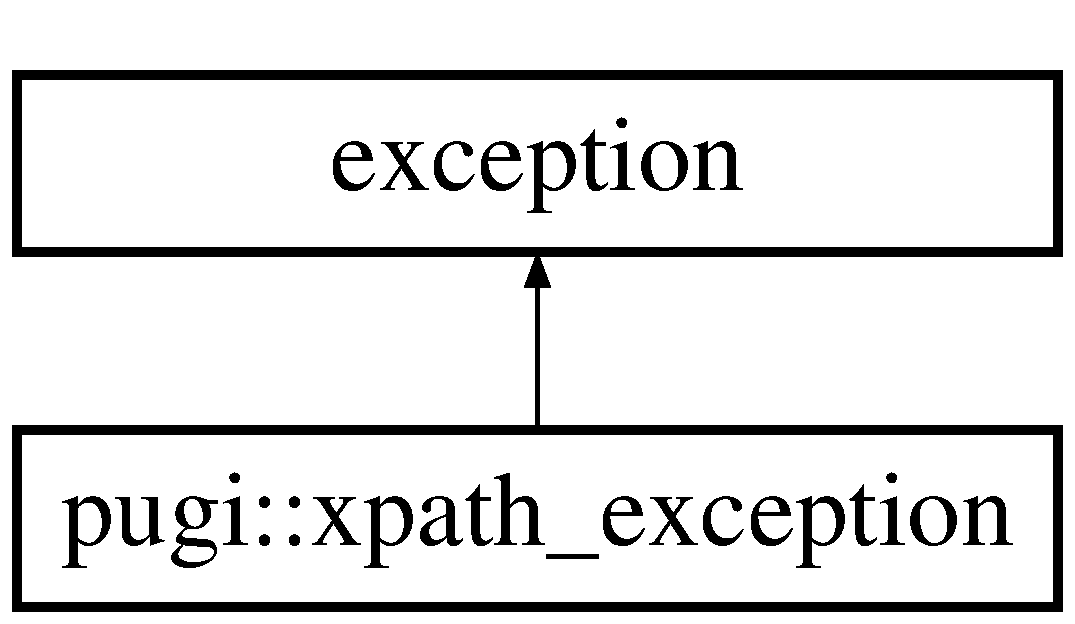
\includegraphics[height=2.000000cm]{classpugi_1_1xpath__exception}
\end{center}
\end{figure}
\subsection*{Public Member Functions}
\begin{DoxyCompactItemize}
\item 
\hyperlink{classpugi_1_1xpath__exception_a67698821481b5a73213d21a1ac174410}{xpath\-\_\-exception} (const \hyperlink{structpugi_1_1xpath__parse__result}{xpath\-\_\-parse\-\_\-result} \&\hyperlink{classpugi_1_1xpath__exception_a6602bbd541153f35a44c2233aa7d37de}{result})
\item 
virtual const char $\ast$ \hyperlink{classpugi_1_1xpath__exception_a986ab92474fa82507981c76ed115ccbd}{what} () const   throw ()
\item 
const \hyperlink{structpugi_1_1xpath__parse__result}{xpath\-\_\-parse\-\_\-result} \& \hyperlink{classpugi_1_1xpath__exception_a6602bbd541153f35a44c2233aa7d37de}{result} () const 
\end{DoxyCompactItemize}


\subsection{Constructor \& Destructor Documentation}
\hypertarget{classpugi_1_1xpath__exception_a67698821481b5a73213d21a1ac174410}{\index{pugi\-::xpath\-\_\-exception@{pugi\-::xpath\-\_\-exception}!xpath\-\_\-exception@{xpath\-\_\-exception}}
\index{xpath\-\_\-exception@{xpath\-\_\-exception}!pugi::xpath_exception@{pugi\-::xpath\-\_\-exception}}
\subsubsection[{xpath\-\_\-exception}]{\setlength{\rightskip}{0pt plus 5cm}{\bf P\-U\-G\-I\-\_\-\-\_\-\-F\-N} pugi\-::xpath\-\_\-exception\-::xpath\-\_\-exception (
\begin{DoxyParamCaption}
\item[{const {\bf xpath\-\_\-parse\-\_\-result} \&}]{result}
\end{DoxyParamCaption}
)\hspace{0.3cm}{\ttfamily [explicit]}}}\label{classpugi_1_1xpath__exception_a67698821481b5a73213d21a1ac174410}

\begin{DoxyCode}
9628                                                                               : \_result(result\_)
9629     \{
9630         assert(\_result.\hyperlink{structpugi_1_1xpath__parse__result_ab2c625be89b995afac829012bc749fe4}{error});
9631     \}
\end{DoxyCode}


\subsection{Member Function Documentation}
\hypertarget{classpugi_1_1xpath__exception_a6602bbd541153f35a44c2233aa7d37de}{\index{pugi\-::xpath\-\_\-exception@{pugi\-::xpath\-\_\-exception}!result@{result}}
\index{result@{result}!pugi::xpath_exception@{pugi\-::xpath\-\_\-exception}}
\subsubsection[{result}]{\setlength{\rightskip}{0pt plus 5cm}{\bf P\-U\-G\-I\-\_\-\-\_\-\-F\-N} const {\bf xpath\-\_\-parse\-\_\-result} \& pugi\-::xpath\-\_\-exception\-::result (
\begin{DoxyParamCaption}
{}
\end{DoxyParamCaption}
) const}}\label{classpugi_1_1xpath__exception_a6602bbd541153f35a44c2233aa7d37de}

\begin{DoxyCode}
9639     \{
9640         \textcolor{keywordflow}{return} \_result;
9641     \}
\end{DoxyCode}
\hypertarget{classpugi_1_1xpath__exception_a986ab92474fa82507981c76ed115ccbd}{\index{pugi\-::xpath\-\_\-exception@{pugi\-::xpath\-\_\-exception}!what@{what}}
\index{what@{what}!pugi::xpath_exception@{pugi\-::xpath\-\_\-exception}}
\subsubsection[{what}]{\setlength{\rightskip}{0pt plus 5cm}{\bf P\-U\-G\-I\-\_\-\-\_\-\-F\-N} const char $\ast$ pugi\-::xpath\-\_\-exception\-::what (
\begin{DoxyParamCaption}
{}
\end{DoxyParamCaption}
) const throw  ) \hspace{0.3cm}{\ttfamily [virtual]}}}\label{classpugi_1_1xpath__exception_a986ab92474fa82507981c76ed115ccbd}

\begin{DoxyCode}
9634     \{
9635         \textcolor{keywordflow}{return} \_result.\hyperlink{structpugi_1_1xpath__parse__result_ab2c625be89b995afac829012bc749fe4}{error};
9636     \}
\end{DoxyCode}


The documentation for this class was generated from the following files\-:\begin{DoxyCompactItemize}
\item 
Third\-Party/pugixml/\hyperlink{pugixml_8hpp}{pugixml.\-hpp}\item 
Third\-Party/pugixml/\hyperlink{pugixml_8cpp}{pugixml.\-cpp}\end{DoxyCompactItemize}

\hypertarget{classxpath__lexer}{\section{xpath\-\_\-lexer Class Reference}
\label{classxpath__lexer}\index{xpath\-\_\-lexer@{xpath\-\_\-lexer}}
}
\subsection*{Public Member Functions}
\begin{DoxyCompactItemize}
\item 
\hyperlink{classxpath__lexer_aa52661c9ba7dfa262d3ab49f578653c3}{xpath\-\_\-lexer} (const char\-\_\-t $\ast$query)
\item 
const char\-\_\-t $\ast$ \hyperlink{classxpath__lexer_a3794e29f3bec2fa31346766eea978cbf}{state} () const 
\item 
void \hyperlink{classxpath__lexer_a32684b3097fccb4d626da620b44b72ad}{next} ()
\item 
\hyperlink{pugixml_8cpp_a1fdd6d0a63acbba1491ab331ddce4ac9}{lexeme\-\_\-t} \hyperlink{classxpath__lexer_a06cdc258948ef3a1a69bd7d5733fd987}{current} () const 
\item 
const char\-\_\-t $\ast$ \hyperlink{classxpath__lexer_a7adef722d64938e3ba79ae1a7e1c0d71}{current\-\_\-pos} () const 
\item 
const \hyperlink{structxpath__lexer__string}{xpath\-\_\-lexer\-\_\-string} \& \hyperlink{classxpath__lexer_aebb02b6d507f5e0839bfa42116bdbc9c}{contents} () const 
\end{DoxyCompactItemize}


\subsection{Constructor \& Destructor Documentation}
\hypertarget{classxpath__lexer_aa52661c9ba7dfa262d3ab49f578653c3}{\index{xpath\-\_\-lexer@{xpath\-\_\-lexer}!xpath\-\_\-lexer@{xpath\-\_\-lexer}}
\index{xpath\-\_\-lexer@{xpath\-\_\-lexer}!xpath_lexer@{xpath\-\_\-lexer}}
\subsubsection[{xpath\-\_\-lexer}]{\setlength{\rightskip}{0pt plus 5cm}xpath\-\_\-lexer\-::xpath\-\_\-lexer (
\begin{DoxyParamCaption}
\item[{const char\-\_\-t $\ast$}]{query}
\end{DoxyParamCaption}
)\hspace{0.3cm}{\ttfamily [inline]}, {\ttfamily [explicit]}}}\label{classxpath__lexer_aa52661c9ba7dfa262d3ab49f578653c3}

\begin{DoxyCode}
6982                                                  : \_cur(query)
6983         \{
6984             \hyperlink{classxpath__lexer_a32684b3097fccb4d626da620b44b72ad}{next}();
6985         \}
\end{DoxyCode}


\subsection{Member Function Documentation}
\hypertarget{classxpath__lexer_aebb02b6d507f5e0839bfa42116bdbc9c}{\index{xpath\-\_\-lexer@{xpath\-\_\-lexer}!contents@{contents}}
\index{contents@{contents}!xpath_lexer@{xpath\-\_\-lexer}}
\subsubsection[{contents}]{\setlength{\rightskip}{0pt plus 5cm}const {\bf xpath\-\_\-lexer\-\_\-string}\& xpath\-\_\-lexer\-::contents (
\begin{DoxyParamCaption}
{}
\end{DoxyParamCaption}
) const\hspace{0.3cm}{\ttfamily [inline]}}}\label{classxpath__lexer_aebb02b6d507f5e0839bfa42116bdbc9c}

\begin{DoxyCode}
7272         \{
7273             assert(\_cur\_lexeme == \hyperlink{pugixml_8cpp_a1fdd6d0a63acbba1491ab331ddce4ac9a933a0fd7c93a22506dc917d0868e05d1}{lex\_var\_ref} || \_cur\_lexeme == 
      \hyperlink{pugixml_8cpp_a1fdd6d0a63acbba1491ab331ddce4ac9abe562e581d64a34b55b3d9b38db2e480}{lex\_number} || \_cur\_lexeme == \hyperlink{pugixml_8cpp_a1fdd6d0a63acbba1491ab331ddce4ac9aa18bda8e798cdf55d88ed65fd025e67c}{lex\_string} || \_cur\_lexeme == 
      \hyperlink{pugixml_8cpp_a1fdd6d0a63acbba1491ab331ddce4ac9a1f793e76227244d2ae78acf451b82808}{lex\_quoted\_string});
7274 
7275             \textcolor{keywordflow}{return} \_cur\_lexeme\_contents;
7276         \}
\end{DoxyCode}
\hypertarget{classxpath__lexer_a06cdc258948ef3a1a69bd7d5733fd987}{\index{xpath\-\_\-lexer@{xpath\-\_\-lexer}!current@{current}}
\index{current@{current}!xpath_lexer@{xpath\-\_\-lexer}}
\subsubsection[{current}]{\setlength{\rightskip}{0pt plus 5cm}{\bf lexeme\-\_\-t} xpath\-\_\-lexer\-::current (
\begin{DoxyParamCaption}
{}
\end{DoxyParamCaption}
) const\hspace{0.3cm}{\ttfamily [inline]}}}\label{classxpath__lexer_a06cdc258948ef3a1a69bd7d5733fd987}

\begin{DoxyCode}
7262         \{
7263             \textcolor{keywordflow}{return} \_cur\_lexeme;
7264         \}
\end{DoxyCode}
\hypertarget{classxpath__lexer_a7adef722d64938e3ba79ae1a7e1c0d71}{\index{xpath\-\_\-lexer@{xpath\-\_\-lexer}!current\-\_\-pos@{current\-\_\-pos}}
\index{current\-\_\-pos@{current\-\_\-pos}!xpath_lexer@{xpath\-\_\-lexer}}
\subsubsection[{current\-\_\-pos}]{\setlength{\rightskip}{0pt plus 5cm}const char\-\_\-t$\ast$ xpath\-\_\-lexer\-::current\-\_\-pos (
\begin{DoxyParamCaption}
{}
\end{DoxyParamCaption}
) const\hspace{0.3cm}{\ttfamily [inline]}}}\label{classxpath__lexer_a7adef722d64938e3ba79ae1a7e1c0d71}

\begin{DoxyCode}
7267         \{
7268             \textcolor{keywordflow}{return} \_cur\_lexeme\_pos;
7269         \}
\end{DoxyCode}
\hypertarget{classxpath__lexer_a32684b3097fccb4d626da620b44b72ad}{\index{xpath\-\_\-lexer@{xpath\-\_\-lexer}!next@{next}}
\index{next@{next}!xpath_lexer@{xpath\-\_\-lexer}}
\subsubsection[{next}]{\setlength{\rightskip}{0pt plus 5cm}void xpath\-\_\-lexer\-::next (
\begin{DoxyParamCaption}
{}
\end{DoxyParamCaption}
)\hspace{0.3cm}{\ttfamily [inline]}}}\label{classxpath__lexer_a32684b3097fccb4d626da620b44b72ad}

\begin{DoxyCode}
6993         \{
6994             \textcolor{keyword}{const} \hyperlink{namespacepugi_aef5a7a62cba0507542220ea15afe39df}{char\_t}* cur = \_cur;
6995 
6996             \textcolor{keywordflow}{while} (\hyperlink{pugixml_8cpp_a2adf5ae9b7505408a18e9f3bb1b3d332}{PUGI\_\_IS\_CHARTYPE}(*cur, \hyperlink{pugixml_8cpp_ae83a55e5947d28c62625b690b1484108ac957a1774b6a4430e583bcb881909372}{ct\_space})) ++cur;
6997 
6998             \textcolor{comment}{// save lexeme position for error reporting}
6999             \_cur\_lexeme\_pos = cur;
7000 
7001             \textcolor{keywordflow}{switch} (*cur)
7002             \{
7003             \textcolor{keywordflow}{case} 0:
7004                 \_cur\_lexeme = \hyperlink{pugixml_8cpp_a1fdd6d0a63acbba1491ab331ddce4ac9aade5d69e447274d8785ebc7d438be522}{lex\_eof};
7005                 \textcolor{keywordflow}{break};
7006             
7007             \textcolor{keywordflow}{case} \textcolor{charliteral}{'>'}:
7008                 \textcolor{keywordflow}{if} (*(cur+1) == \textcolor{charliteral}{'='})
7009                 \{
7010                     cur += 2;
7011                     \_cur\_lexeme = \hyperlink{pugixml_8cpp_a1fdd6d0a63acbba1491ab331ddce4ac9a6308ad256806534e1cd586574718a562}{lex\_greater\_or\_equal};
7012                 \}
7013                 \textcolor{keywordflow}{else}
7014                 \{
7015                     cur += 1;
7016                     \_cur\_lexeme = \hyperlink{pugixml_8cpp_a1fdd6d0a63acbba1491ab331ddce4ac9abef050e09f087253f62bd3b4b6b435af}{lex\_greater};
7017                 \}
7018                 \textcolor{keywordflow}{break};
7019 
7020             \textcolor{keywordflow}{case} \textcolor{charliteral}{'<'}:
7021                 \textcolor{keywordflow}{if} (*(cur+1) == \textcolor{charliteral}{'='})
7022                 \{
7023                     cur += 2;
7024                     \_cur\_lexeme = \hyperlink{pugixml_8cpp_a1fdd6d0a63acbba1491ab331ddce4ac9acd542cd6bfd08efcfa647426a7d577b8}{lex\_less\_or\_equal};
7025                 \}
7026                 \textcolor{keywordflow}{else}
7027                 \{
7028                     cur += 1;
7029                     \_cur\_lexeme = \hyperlink{pugixml_8cpp_a1fdd6d0a63acbba1491ab331ddce4ac9a51a5852f31a8c2bd889f340ac3ab9fe4}{lex\_less};
7030                 \}
7031                 \textcolor{keywordflow}{break};
7032 
7033             \textcolor{keywordflow}{case} \textcolor{charliteral}{'!'}:
7034                 \textcolor{keywordflow}{if} (*(cur+1) == \textcolor{charliteral}{'='})
7035                 \{
7036                     cur += 2;
7037                     \_cur\_lexeme = \hyperlink{pugixml_8cpp_a1fdd6d0a63acbba1491ab331ddce4ac9a266a8f8365e61873ecb66c78d363f156}{lex\_not\_equal};
7038                 \}
7039                 \textcolor{keywordflow}{else}
7040                 \{
7041                     \_cur\_lexeme = \hyperlink{pugixml_8cpp_a1fdd6d0a63acbba1491ab331ddce4ac9a6696dceb02e4d282197154d3805e8ce1}{lex\_none};
7042                 \}
7043                 \textcolor{keywordflow}{break};
7044 
7045             \textcolor{keywordflow}{case} \textcolor{charliteral}{'='}:
7046                 cur += 1;
7047                 \_cur\_lexeme = \hyperlink{pugixml_8cpp_a1fdd6d0a63acbba1491ab331ddce4ac9a5c2d9372cf8440a68eff3c16eeac8027}{lex\_equal};
7048 
7049                 \textcolor{keywordflow}{break};
7050             
7051             \textcolor{keywordflow}{case} \textcolor{charliteral}{'+'}:
7052                 cur += 1;
7053                 \_cur\_lexeme = \hyperlink{pugixml_8cpp_a1fdd6d0a63acbba1491ab331ddce4ac9ab165cbd439d1c24dd336e02645c98727}{lex\_plus};
7054 
7055                 \textcolor{keywordflow}{break};
7056 
7057             \textcolor{keywordflow}{case} \textcolor{charliteral}{'-'}:
7058                 cur += 1;
7059                 \_cur\_lexeme = \hyperlink{pugixml_8cpp_a1fdd6d0a63acbba1491ab331ddce4ac9aa0a1d6df3298c5b043daa6ad9afa2733}{lex\_minus};
7060 
7061                 \textcolor{keywordflow}{break};
7062 
7063             \textcolor{keywordflow}{case} \textcolor{charliteral}{'*'}:
7064                 cur += 1;
7065                 \_cur\_lexeme = \hyperlink{pugixml_8cpp_a1fdd6d0a63acbba1491ab331ddce4ac9a095a092388d76a21ccfc1338c875fe54}{lex\_multiply};
7066 
7067                 \textcolor{keywordflow}{break};
7068 
7069             \textcolor{keywordflow}{case} \textcolor{charliteral}{'|'}:
7070                 cur += 1;
7071                 \_cur\_lexeme = \hyperlink{pugixml_8cpp_a1fdd6d0a63acbba1491ab331ddce4ac9a751c2248d5cb85f4ba650a78281923a1}{lex\_union};
7072 
7073                 \textcolor{keywordflow}{break};
7074             
7075             \textcolor{keywordflow}{case} \textcolor{charliteral}{'$'}:
7076                 cur += 1;
7077 
7078                 \textcolor{keywordflow}{if} (\hyperlink{pugixml_8cpp_a4ce684b35edc78e6fda91e836f29a46c}{PUGI\_\_IS\_CHARTYPEX}(*cur, \hyperlink{pugixml_8cpp_af8255f70e16ba8c6dbd5ff66cef9af26a934b9be54f1b4446a7a6665373d50ad6}{ctx\_start\_symbol}))
7079                 \{
7080                     \_cur\_lexeme\_contents.\hyperlink{structxpath__lexer__string_a0b985863d7363a75d4fdd0a7ece1fca0}{begin} = cur;
7081 
7082                     \textcolor{keywordflow}{while} (\hyperlink{pugixml_8cpp_a4ce684b35edc78e6fda91e836f29a46c}{PUGI\_\_IS\_CHARTYPEX}(*cur, \hyperlink{pugixml_8cpp_af8255f70e16ba8c6dbd5ff66cef9af26a7f60ee1dbb91625306756d7b8289162e}{ctx\_symbol})) cur++;
7083 
7084                     \textcolor{keywordflow}{if} (cur[0] == \textcolor{charliteral}{':'} && \hyperlink{pugixml_8cpp_a4ce684b35edc78e6fda91e836f29a46c}{PUGI\_\_IS\_CHARTYPEX}(cur[1], 
      \hyperlink{pugixml_8cpp_af8255f70e16ba8c6dbd5ff66cef9af26a7f60ee1dbb91625306756d7b8289162e}{ctx\_symbol})) \textcolor{comment}{// qname}
7085                     \{
7086                         cur++; \textcolor{comment}{// :}
7087 
7088                         \textcolor{keywordflow}{while} (\hyperlink{pugixml_8cpp_a4ce684b35edc78e6fda91e836f29a46c}{PUGI\_\_IS\_CHARTYPEX}(*cur, 
      \hyperlink{pugixml_8cpp_af8255f70e16ba8c6dbd5ff66cef9af26a7f60ee1dbb91625306756d7b8289162e}{ctx\_symbol})) cur++;
7089                     \}
7090 
7091                     \_cur\_lexeme\_contents.\hyperlink{structxpath__lexer__string_a13bbedeca2f8c2fb1e294325eea66878}{end} = cur;
7092                 
7093                     \_cur\_lexeme = \hyperlink{pugixml_8cpp_a1fdd6d0a63acbba1491ab331ddce4ac9a933a0fd7c93a22506dc917d0868e05d1}{lex\_var\_ref};
7094                 \}
7095                 \textcolor{keywordflow}{else}
7096                 \{
7097                     \_cur\_lexeme = \hyperlink{pugixml_8cpp_a1fdd6d0a63acbba1491ab331ddce4ac9a6696dceb02e4d282197154d3805e8ce1}{lex\_none};
7098                 \}
7099 
7100                 \textcolor{keywordflow}{break};
7101 
7102             \textcolor{keywordflow}{case} \textcolor{charliteral}{'('}:
7103                 cur += 1;
7104                 \_cur\_lexeme = \hyperlink{pugixml_8cpp_a1fdd6d0a63acbba1491ab331ddce4ac9aea53091cdb9dce7a878792f2c8d4d17b}{lex\_open\_brace};
7105 
7106                 \textcolor{keywordflow}{break};
7107 
7108             \textcolor{keywordflow}{case} \textcolor{charliteral}{')'}:
7109                 cur += 1;
7110                 \_cur\_lexeme = \hyperlink{pugixml_8cpp_a1fdd6d0a63acbba1491ab331ddce4ac9a8a39009230ffa4187d22c91412f7fcd7}{lex\_close\_brace};
7111 
7112                 \textcolor{keywordflow}{break};
7113             
7114             \textcolor{keywordflow}{case} \textcolor{charliteral}{'['}:
7115                 cur += 1;
7116                 \_cur\_lexeme = \hyperlink{pugixml_8cpp_a1fdd6d0a63acbba1491ab331ddce4ac9ad9321b18d06078ecc38ad112ce654ce9}{lex\_open\_square\_brace};
7117 
7118                 \textcolor{keywordflow}{break};
7119 
7120             \textcolor{keywordflow}{case} \textcolor{charliteral}{']'}:
7121                 cur += 1;
7122                 \_cur\_lexeme = \hyperlink{pugixml_8cpp_a1fdd6d0a63acbba1491ab331ddce4ac9ad572f5fa18506a8bf523425d075cac5d}{lex\_close\_square\_brace};
7123 
7124                 \textcolor{keywordflow}{break};
7125 
7126             \textcolor{keywordflow}{case} \textcolor{charliteral}{','}:
7127                 cur += 1;
7128                 \_cur\_lexeme = \hyperlink{pugixml_8cpp_a1fdd6d0a63acbba1491ab331ddce4ac9a78c1259369ef92b19f0ea2701d9c1d60}{lex\_comma};
7129 
7130                 \textcolor{keywordflow}{break};
7131 
7132             \textcolor{keywordflow}{case} \textcolor{charliteral}{'/'}:
7133                 \textcolor{keywordflow}{if} (*(cur+1) == \textcolor{charliteral}{'/'})
7134                 \{
7135                     cur += 2;
7136                     \_cur\_lexeme = \hyperlink{pugixml_8cpp_a1fdd6d0a63acbba1491ab331ddce4ac9a0988911f62781c4a1e8831a76c1e1fe8}{lex\_double\_slash};
7137                 \}
7138                 \textcolor{keywordflow}{else}
7139                 \{
7140                     cur += 1;
7141                     \_cur\_lexeme = \hyperlink{pugixml_8cpp_a1fdd6d0a63acbba1491ab331ddce4ac9a8be0786f2c3130ad30b61bbac70fa809}{lex\_slash};
7142                 \}
7143                 \textcolor{keywordflow}{break};
7144         
7145             \textcolor{keywordflow}{case} \textcolor{charliteral}{'.'}:
7146                 \textcolor{keywordflow}{if} (*(cur+1) == \textcolor{charliteral}{'.'})
7147                 \{
7148                     cur += 2;
7149                     \_cur\_lexeme = \hyperlink{pugixml_8cpp_a1fdd6d0a63acbba1491ab331ddce4ac9abf40f90b4cc064d49394e974962b111b}{lex\_double\_dot};
7150                 \}
7151                 \textcolor{keywordflow}{else} \textcolor{keywordflow}{if} (\hyperlink{pugixml_8cpp_a4ce684b35edc78e6fda91e836f29a46c}{PUGI\_\_IS\_CHARTYPEX}(*(cur+1), 
      \hyperlink{pugixml_8cpp_af8255f70e16ba8c6dbd5ff66cef9af26a1e66040284fe331a2ec2162b6b9fee6a}{ctx\_digit}))
7152                 \{
7153                     \_cur\_lexeme\_contents.\hyperlink{structxpath__lexer__string_a0b985863d7363a75d4fdd0a7ece1fca0}{begin} = cur; \textcolor{comment}{// .}
7154 
7155                     ++cur;
7156 
7157                     \textcolor{keywordflow}{while} (\hyperlink{pugixml_8cpp_a4ce684b35edc78e6fda91e836f29a46c}{PUGI\_\_IS\_CHARTYPEX}(*cur, \hyperlink{pugixml_8cpp_af8255f70e16ba8c6dbd5ff66cef9af26a1e66040284fe331a2ec2162b6b9fee6a}{ctx\_digit})) cur++;
7158 
7159                     \_cur\_lexeme\_contents.\hyperlink{structxpath__lexer__string_a13bbedeca2f8c2fb1e294325eea66878}{end} = cur;
7160                     
7161                     \_cur\_lexeme = \hyperlink{pugixml_8cpp_a1fdd6d0a63acbba1491ab331ddce4ac9abe562e581d64a34b55b3d9b38db2e480}{lex\_number};
7162                 \}
7163                 \textcolor{keywordflow}{else}
7164                 \{
7165                     cur += 1;
7166                     \_cur\_lexeme = \hyperlink{pugixml_8cpp_a1fdd6d0a63acbba1491ab331ddce4ac9aa0709f7aad925098c9b62379206a536b}{lex\_dot};
7167                 \}
7168                 \textcolor{keywordflow}{break};
7169 
7170             \textcolor{keywordflow}{case} \textcolor{charliteral}{'@'}:
7171                 cur += 1;
7172                 \_cur\_lexeme = \hyperlink{pugixml_8cpp_a1fdd6d0a63acbba1491ab331ddce4ac9a408fe857bc6c9b3a148ab798d0ad34e7}{lex\_axis\_attribute};
7173 
7174                 \textcolor{keywordflow}{break};
7175 
7176             \textcolor{keywordflow}{case} \textcolor{charliteral}{'"'}:
7177             \textcolor{keywordflow}{case} \textcolor{charliteral}{'\(\backslash\)''}:
7178             \{
7179                 \hyperlink{namespacepugi_aef5a7a62cba0507542220ea15afe39df}{char\_t} terminator = *cur;
7180 
7181                 ++cur;
7182 
7183                 \_cur\_lexeme\_contents.\hyperlink{structxpath__lexer__string_a0b985863d7363a75d4fdd0a7ece1fca0}{begin} = cur;
7184                 \textcolor{keywordflow}{while} (*cur && *cur != terminator) cur++;
7185                 \_cur\_lexeme\_contents.\hyperlink{structxpath__lexer__string_a13bbedeca2f8c2fb1e294325eea66878}{end} = cur;
7186                 
7187                 \textcolor{keywordflow}{if} (!*cur)
7188                     \_cur\_lexeme = \hyperlink{pugixml_8cpp_a1fdd6d0a63acbba1491ab331ddce4ac9a6696dceb02e4d282197154d3805e8ce1}{lex\_none};
7189                 \textcolor{keywordflow}{else}
7190                 \{
7191                     cur += 1;
7192                     \_cur\_lexeme = \hyperlink{pugixml_8cpp_a1fdd6d0a63acbba1491ab331ddce4ac9a1f793e76227244d2ae78acf451b82808}{lex\_quoted\_string};
7193                 \}
7194 
7195                 \textcolor{keywordflow}{break};
7196             \}
7197 
7198             \textcolor{keywordflow}{case} \textcolor{charliteral}{':'}:
7199                 \textcolor{keywordflow}{if} (*(cur+1) == \textcolor{charliteral}{':'})
7200                 \{
7201                     cur += 2;
7202                     \_cur\_lexeme = \hyperlink{pugixml_8cpp_a1fdd6d0a63acbba1491ab331ddce4ac9afbd9c771f4154c9cf363ff3c0b9f7b9c}{lex\_double\_colon};
7203                 \}
7204                 \textcolor{keywordflow}{else}
7205                 \{
7206                     \_cur\_lexeme = \hyperlink{pugixml_8cpp_a1fdd6d0a63acbba1491ab331ddce4ac9a6696dceb02e4d282197154d3805e8ce1}{lex\_none};
7207                 \}
7208                 \textcolor{keywordflow}{break};
7209 
7210             \textcolor{keywordflow}{default}:
7211                 \textcolor{keywordflow}{if} (\hyperlink{pugixml_8cpp_a4ce684b35edc78e6fda91e836f29a46c}{PUGI\_\_IS\_CHARTYPEX}(*cur, \hyperlink{pugixml_8cpp_af8255f70e16ba8c6dbd5ff66cef9af26a1e66040284fe331a2ec2162b6b9fee6a}{ctx\_digit}))
7212                 \{
7213                     \_cur\_lexeme\_contents.\hyperlink{structxpath__lexer__string_a0b985863d7363a75d4fdd0a7ece1fca0}{begin} = cur;
7214 
7215                     \textcolor{keywordflow}{while} (\hyperlink{pugixml_8cpp_a4ce684b35edc78e6fda91e836f29a46c}{PUGI\_\_IS\_CHARTYPEX}(*cur, \hyperlink{pugixml_8cpp_af8255f70e16ba8c6dbd5ff66cef9af26a1e66040284fe331a2ec2162b6b9fee6a}{ctx\_digit})) cur++;
7216                 
7217                     \textcolor{keywordflow}{if} (*cur == \textcolor{charliteral}{'.'})
7218                     \{
7219                         cur++;
7220 
7221                         \textcolor{keywordflow}{while} (\hyperlink{pugixml_8cpp_a4ce684b35edc78e6fda91e836f29a46c}{PUGI\_\_IS\_CHARTYPEX}(*cur, 
      \hyperlink{pugixml_8cpp_af8255f70e16ba8c6dbd5ff66cef9af26a1e66040284fe331a2ec2162b6b9fee6a}{ctx\_digit})) cur++;
7222                     \}
7223 
7224                     \_cur\_lexeme\_contents.\hyperlink{structxpath__lexer__string_a13bbedeca2f8c2fb1e294325eea66878}{end} = cur;
7225 
7226                     \_cur\_lexeme = \hyperlink{pugixml_8cpp_a1fdd6d0a63acbba1491ab331ddce4ac9abe562e581d64a34b55b3d9b38db2e480}{lex\_number};
7227                 \}
7228                 \textcolor{keywordflow}{else} \textcolor{keywordflow}{if} (\hyperlink{pugixml_8cpp_a4ce684b35edc78e6fda91e836f29a46c}{PUGI\_\_IS\_CHARTYPEX}(*cur, 
      \hyperlink{pugixml_8cpp_af8255f70e16ba8c6dbd5ff66cef9af26a934b9be54f1b4446a7a6665373d50ad6}{ctx\_start\_symbol}))
7229                 \{
7230                     \_cur\_lexeme\_contents.\hyperlink{structxpath__lexer__string_a0b985863d7363a75d4fdd0a7ece1fca0}{begin} = cur;
7231 
7232                     \textcolor{keywordflow}{while} (\hyperlink{pugixml_8cpp_a4ce684b35edc78e6fda91e836f29a46c}{PUGI\_\_IS\_CHARTYPEX}(*cur, \hyperlink{pugixml_8cpp_af8255f70e16ba8c6dbd5ff66cef9af26a7f60ee1dbb91625306756d7b8289162e}{ctx\_symbol})) cur++;
7233 
7234                     \textcolor{keywordflow}{if} (cur[0] == \textcolor{charliteral}{':'})
7235                     \{
7236                         \textcolor{keywordflow}{if} (cur[1] == \textcolor{charliteral}{'*'}) \textcolor{comment}{// namespace test ncname:*}
7237                         \{
7238                             cur += 2; \textcolor{comment}{// :*}
7239                         \}
7240                         \textcolor{keywordflow}{else} \textcolor{keywordflow}{if} (\hyperlink{pugixml_8cpp_a4ce684b35edc78e6fda91e836f29a46c}{PUGI\_\_IS\_CHARTYPEX}(cur[1], 
      \hyperlink{pugixml_8cpp_af8255f70e16ba8c6dbd5ff66cef9af26a7f60ee1dbb91625306756d7b8289162e}{ctx\_symbol})) \textcolor{comment}{// namespace test qname}
7241                         \{
7242                             cur++; \textcolor{comment}{// :}
7243 
7244                             \textcolor{keywordflow}{while} (\hyperlink{pugixml_8cpp_a4ce684b35edc78e6fda91e836f29a46c}{PUGI\_\_IS\_CHARTYPEX}(*cur, 
      \hyperlink{pugixml_8cpp_af8255f70e16ba8c6dbd5ff66cef9af26a7f60ee1dbb91625306756d7b8289162e}{ctx\_symbol})) cur++;
7245                         \}
7246                     \}
7247 
7248                     \_cur\_lexeme\_contents.\hyperlink{structxpath__lexer__string_a13bbedeca2f8c2fb1e294325eea66878}{end} = cur;
7249                 
7250                     \_cur\_lexeme = \hyperlink{pugixml_8cpp_a1fdd6d0a63acbba1491ab331ddce4ac9aa18bda8e798cdf55d88ed65fd025e67c}{lex\_string};
7251                 \}
7252                 \textcolor{keywordflow}{else}
7253                 \{
7254                     \_cur\_lexeme = \hyperlink{pugixml_8cpp_a1fdd6d0a63acbba1491ab331ddce4ac9a6696dceb02e4d282197154d3805e8ce1}{lex\_none};
7255                 \}
7256             \}
7257 
7258             \_cur = cur;
7259         \}
\end{DoxyCode}
\hypertarget{classxpath__lexer_a3794e29f3bec2fa31346766eea978cbf}{\index{xpath\-\_\-lexer@{xpath\-\_\-lexer}!state@{state}}
\index{state@{state}!xpath_lexer@{xpath\-\_\-lexer}}
\subsubsection[{state}]{\setlength{\rightskip}{0pt plus 5cm}const char\-\_\-t$\ast$ xpath\-\_\-lexer\-::state (
\begin{DoxyParamCaption}
{}
\end{DoxyParamCaption}
) const\hspace{0.3cm}{\ttfamily [inline]}}}\label{classxpath__lexer_a3794e29f3bec2fa31346766eea978cbf}

\begin{DoxyCode}
6988         \{
6989             \textcolor{keywordflow}{return} \_cur;
6990         \}
\end{DoxyCode}


The documentation for this class was generated from the following file\-:\begin{DoxyCompactItemize}
\item 
Third\-Party/pugixml/\hyperlink{pugixml_8cpp}{pugixml.\-cpp}\end{DoxyCompactItemize}

\hypertarget{structxpath__lexer__string}{\section{xpath\-\_\-lexer\-\_\-string Struct Reference}
\label{structxpath__lexer__string}\index{xpath\-\_\-lexer\-\_\-string@{xpath\-\_\-lexer\-\_\-string}}
}
\subsection*{Public Member Functions}
\begin{DoxyCompactItemize}
\item 
\hyperlink{structxpath__lexer__string_a3e60ca9bfea3cf907582eb527479e304}{xpath\-\_\-lexer\-\_\-string} ()
\item 
bool \hyperlink{structxpath__lexer__string_ac19adfd75832be8eff3f430aa3cb3c14}{operator==} (const char\-\_\-t $\ast$other) const 
\end{DoxyCompactItemize}
\subsection*{Data Fields}
\begin{DoxyCompactItemize}
\item 
const char\-\_\-t $\ast$ \hyperlink{structxpath__lexer__string_a0b985863d7363a75d4fdd0a7ece1fca0}{begin}
\item 
const char\-\_\-t $\ast$ \hyperlink{structxpath__lexer__string_a13bbedeca2f8c2fb1e294325eea66878}{end}
\end{DoxyCompactItemize}


\subsection{Constructor \& Destructor Documentation}
\hypertarget{structxpath__lexer__string_a3e60ca9bfea3cf907582eb527479e304}{\index{xpath\-\_\-lexer\-\_\-string@{xpath\-\_\-lexer\-\_\-string}!xpath\-\_\-lexer\-\_\-string@{xpath\-\_\-lexer\-\_\-string}}
\index{xpath\-\_\-lexer\-\_\-string@{xpath\-\_\-lexer\-\_\-string}!xpath_lexer_string@{xpath\-\_\-lexer\-\_\-string}}
\subsubsection[{xpath\-\_\-lexer\-\_\-string}]{\setlength{\rightskip}{0pt plus 5cm}xpath\-\_\-lexer\-\_\-string\-::xpath\-\_\-lexer\-\_\-string (
\begin{DoxyParamCaption}
{}
\end{DoxyParamCaption}
)\hspace{0.3cm}{\ttfamily [inline]}}}\label{structxpath__lexer__string_a3e60ca9bfea3cf907582eb527479e304}

\begin{DoxyCode}
6961                             : \hyperlink{structxpath__lexer__string_a0b985863d7363a75d4fdd0a7ece1fca0}{begin}(0), \hyperlink{structxpath__lexer__string_a13bbedeca2f8c2fb1e294325eea66878}{end}(0)
6962         \{
6963         \}
\end{DoxyCode}


\subsection{Member Function Documentation}
\hypertarget{structxpath__lexer__string_ac19adfd75832be8eff3f430aa3cb3c14}{\index{xpath\-\_\-lexer\-\_\-string@{xpath\-\_\-lexer\-\_\-string}!operator==@{operator==}}
\index{operator==@{operator==}!xpath_lexer_string@{xpath\-\_\-lexer\-\_\-string}}
\subsubsection[{operator==}]{\setlength{\rightskip}{0pt plus 5cm}bool xpath\-\_\-lexer\-\_\-string\-::operator== (
\begin{DoxyParamCaption}
\item[{const char\-\_\-t $\ast$}]{other}
\end{DoxyParamCaption}
) const\hspace{0.3cm}{\ttfamily [inline]}}}\label{structxpath__lexer__string_ac19adfd75832be8eff3f430aa3cb3c14}

\begin{DoxyCode}
6966         \{
6967             \textcolor{keywordtype}{size\_t} length = \textcolor{keyword}{static\_cast<}\textcolor{keywordtype}{size\_t}\textcolor{keyword}{>}(\hyperlink{structxpath__lexer__string_a13bbedeca2f8c2fb1e294325eea66878}{end} - \hyperlink{structxpath__lexer__string_a0b985863d7363a75d4fdd0a7ece1fca0}{begin});
6968 
6969             \textcolor{keywordflow}{return} \hyperlink{pugixml_8cpp_abbf171d1eb53f93f1fa710de5673f889}{strequalrange}(other, \hyperlink{structxpath__lexer__string_a0b985863d7363a75d4fdd0a7ece1fca0}{begin}, length);
6970         \}
\end{DoxyCode}


\subsection{Field Documentation}
\hypertarget{structxpath__lexer__string_a0b985863d7363a75d4fdd0a7ece1fca0}{\index{xpath\-\_\-lexer\-\_\-string@{xpath\-\_\-lexer\-\_\-string}!begin@{begin}}
\index{begin@{begin}!xpath_lexer_string@{xpath\-\_\-lexer\-\_\-string}}
\subsubsection[{begin}]{\setlength{\rightskip}{0pt plus 5cm}const char\-\_\-t$\ast$ xpath\-\_\-lexer\-\_\-string\-::begin}}\label{structxpath__lexer__string_a0b985863d7363a75d4fdd0a7ece1fca0}
\hypertarget{structxpath__lexer__string_a13bbedeca2f8c2fb1e294325eea66878}{\index{xpath\-\_\-lexer\-\_\-string@{xpath\-\_\-lexer\-\_\-string}!end@{end}}
\index{end@{end}!xpath_lexer_string@{xpath\-\_\-lexer\-\_\-string}}
\subsubsection[{end}]{\setlength{\rightskip}{0pt plus 5cm}const char\-\_\-t$\ast$ xpath\-\_\-lexer\-\_\-string\-::end}}\label{structxpath__lexer__string_a13bbedeca2f8c2fb1e294325eea66878}


The documentation for this struct was generated from the following file\-:\begin{DoxyCompactItemize}
\item 
Third\-Party/pugixml/\hyperlink{pugixml_8cpp}{pugixml.\-cpp}\end{DoxyCompactItemize}

\hypertarget{structxpath__memory__block}{\section{xpath\-\_\-memory\-\_\-block Struct Reference}
\label{structxpath__memory__block}\index{xpath\-\_\-memory\-\_\-block@{xpath\-\_\-memory\-\_\-block}}
}
\subsection*{Data Fields}
\begin{DoxyCompactItemize}
\item 
\hyperlink{structxpath__memory__block}{xpath\-\_\-memory\-\_\-block} $\ast$ \hyperlink{structxpath__memory__block_ab7f0d8400b40a51cdb063e76fd19a93c}{next}
\item 
char \hyperlink{structxpath__memory__block_a7b00376d0eac172ab537b6b0964858a9}{data} \mbox{[}4096\mbox{]}
\end{DoxyCompactItemize}


\subsection{Field Documentation}
\hypertarget{structxpath__memory__block_a7b00376d0eac172ab537b6b0964858a9}{\index{xpath\-\_\-memory\-\_\-block@{xpath\-\_\-memory\-\_\-block}!data@{data}}
\index{data@{data}!xpath_memory_block@{xpath\-\_\-memory\-\_\-block}}
\subsubsection[{data}]{\setlength{\rightskip}{0pt plus 5cm}char xpath\-\_\-memory\-\_\-block\-::data\mbox{[}4096\mbox{]}}}\label{structxpath__memory__block_a7b00376d0eac172ab537b6b0964858a9}
\hypertarget{structxpath__memory__block_ab7f0d8400b40a51cdb063e76fd19a93c}{\index{xpath\-\_\-memory\-\_\-block@{xpath\-\_\-memory\-\_\-block}!next@{next}}
\index{next@{next}!xpath_memory_block@{xpath\-\_\-memory\-\_\-block}}
\subsubsection[{next}]{\setlength{\rightskip}{0pt plus 5cm}{\bf xpath\-\_\-memory\-\_\-block}$\ast$ xpath\-\_\-memory\-\_\-block\-::next}}\label{structxpath__memory__block_ab7f0d8400b40a51cdb063e76fd19a93c}


The documentation for this struct was generated from the following file\-:\begin{DoxyCompactItemize}
\item 
Third\-Party/pugixml/\hyperlink{pugixml_8cpp}{pugixml.\-cpp}\end{DoxyCompactItemize}

\hypertarget{classpugi_1_1xpath__node}{\section{pugi\-:\-:xpath\-\_\-node Class Reference}
\label{classpugi_1_1xpath__node}\index{pugi\-::xpath\-\_\-node@{pugi\-::xpath\-\_\-node}}
}


{\ttfamily \#include $<$pugixml.\-hpp$>$}

\subsection*{Public Member Functions}
\begin{DoxyCompactItemize}
\item 
\hyperlink{classpugi_1_1xpath__node_a149bbfe4c145f7ebb8852ae5136ede49}{xpath\-\_\-node} ()
\item 
\hyperlink{classpugi_1_1xpath__node_af35940ce58d68e3210c88c816396c158}{xpath\-\_\-node} (const \hyperlink{classpugi_1_1xml__node}{xml\-\_\-node} \&\hyperlink{classpugi_1_1xpath__node_a5b504b06678b84eedc8467cbd39beb8f}{node})
\item 
\hyperlink{classpugi_1_1xpath__node_a64e77111af6283205e83b97b76d953d0}{xpath\-\_\-node} (const \hyperlink{classpugi_1_1xml__attribute}{xml\-\_\-attribute} \&\hyperlink{classpugi_1_1xpath__node_ad3c5fe70e4293c70451abba5021a9406}{attribute}, const \hyperlink{classpugi_1_1xml__node}{xml\-\_\-node} \&\hyperlink{classpugi_1_1xpath__node_a69d8000479ceddd7c6939c7258f27c39}{parent})
\item 
\hyperlink{classpugi_1_1xml__node}{xml\-\_\-node} \hyperlink{classpugi_1_1xpath__node_a5b504b06678b84eedc8467cbd39beb8f}{node} () const 
\item 
\hyperlink{classpugi_1_1xml__attribute}{xml\-\_\-attribute} \hyperlink{classpugi_1_1xpath__node_ad3c5fe70e4293c70451abba5021a9406}{attribute} () const 
\item 
\hyperlink{classpugi_1_1xml__node}{xml\-\_\-node} \hyperlink{classpugi_1_1xpath__node_a69d8000479ceddd7c6939c7258f27c39}{parent} () const 
\item 
\hyperlink{classpugi_1_1xpath__node_a6e0b138075a145e47dc00a7a17b4ba81}{operator unspecified\-\_\-bool\-\_\-type} () const 
\item 
bool \hyperlink{classpugi_1_1xpath__node_a98167a5daf167fa06dff88b6c4af5646}{operator!} () const 
\item 
bool \hyperlink{classpugi_1_1xpath__node_ac41341c30e66880aad2a731203d9cf4b}{operator==} (const \hyperlink{classpugi_1_1xpath__node}{xpath\-\_\-node} \&n) const 
\item 
bool \hyperlink{classpugi_1_1xpath__node_a785725ca60a15a9d2df83b91725105bd}{operator!=} (const \hyperlink{classpugi_1_1xpath__node}{xpath\-\_\-node} \&n) const 
\end{DoxyCompactItemize}


\subsection{Constructor \& Destructor Documentation}
\hypertarget{classpugi_1_1xpath__node_a149bbfe4c145f7ebb8852ae5136ede49}{\index{pugi\-::xpath\-\_\-node@{pugi\-::xpath\-\_\-node}!xpath\-\_\-node@{xpath\-\_\-node}}
\index{xpath\-\_\-node@{xpath\-\_\-node}!pugi::xpath_node@{pugi\-::xpath\-\_\-node}}
\subsubsection[{xpath\-\_\-node}]{\setlength{\rightskip}{0pt plus 5cm}{\bf P\-U\-G\-I\-\_\-\-\_\-\-F\-N} pugi\-::xpath\-\_\-node\-::xpath\-\_\-node (
\begin{DoxyParamCaption}
{}
\end{DoxyParamCaption}
)}}\label{classpugi_1_1xpath__node_a149bbfe4c145f7ebb8852ae5136ede49}

\begin{DoxyCode}
9645     \{
9646     \}
\end{DoxyCode}
\hypertarget{classpugi_1_1xpath__node_af35940ce58d68e3210c88c816396c158}{\index{pugi\-::xpath\-\_\-node@{pugi\-::xpath\-\_\-node}!xpath\-\_\-node@{xpath\-\_\-node}}
\index{xpath\-\_\-node@{xpath\-\_\-node}!pugi::xpath_node@{pugi\-::xpath\-\_\-node}}
\subsubsection[{xpath\-\_\-node}]{\setlength{\rightskip}{0pt plus 5cm}{\bf P\-U\-G\-I\-\_\-\-\_\-\-F\-N} pugi\-::xpath\-\_\-node\-::xpath\-\_\-node (
\begin{DoxyParamCaption}
\item[{const {\bf xml\-\_\-node} \&}]{node}
\end{DoxyParamCaption}
)}}\label{classpugi_1_1xpath__node_af35940ce58d68e3210c88c816396c158}

\begin{DoxyCode}
9648                                                         : \_node(node\_)
9649     \{
9650     \}
\end{DoxyCode}
\hypertarget{classpugi_1_1xpath__node_a64e77111af6283205e83b97b76d953d0}{\index{pugi\-::xpath\-\_\-node@{pugi\-::xpath\-\_\-node}!xpath\-\_\-node@{xpath\-\_\-node}}
\index{xpath\-\_\-node@{xpath\-\_\-node}!pugi::xpath_node@{pugi\-::xpath\-\_\-node}}
\subsubsection[{xpath\-\_\-node}]{\setlength{\rightskip}{0pt plus 5cm}{\bf P\-U\-G\-I\-\_\-\-\_\-\-F\-N} pugi\-::xpath\-\_\-node\-::xpath\-\_\-node (
\begin{DoxyParamCaption}
\item[{const {\bf xml\-\_\-attribute} \&}]{attribute, }
\item[{const {\bf xml\-\_\-node} \&}]{parent}
\end{DoxyParamCaption}
)}}\label{classpugi_1_1xpath__node_a64e77111af6283205e83b97b76d953d0}

\begin{DoxyCode}
9652                                                                                            : \_node(
      attribute\_ ? parent\_ : xml\_node()), \_attribute(attribute\_)
9653     \{
9654     \}
\end{DoxyCode}


\subsection{Member Function Documentation}
\hypertarget{classpugi_1_1xpath__node_ad3c5fe70e4293c70451abba5021a9406}{\index{pugi\-::xpath\-\_\-node@{pugi\-::xpath\-\_\-node}!attribute@{attribute}}
\index{attribute@{attribute}!pugi::xpath_node@{pugi\-::xpath\-\_\-node}}
\subsubsection[{attribute}]{\setlength{\rightskip}{0pt plus 5cm}{\bf P\-U\-G\-I\-\_\-\-\_\-\-F\-N} {\bf xml\-\_\-attribute} pugi\-::xpath\-\_\-node\-::attribute (
\begin{DoxyParamCaption}
{}
\end{DoxyParamCaption}
) const}}\label{classpugi_1_1xpath__node_ad3c5fe70e4293c70451abba5021a9406}

\begin{DoxyCode}
9662     \{
9663         \textcolor{keywordflow}{return} \_attribute;
9664     \}
\end{DoxyCode}
\hypertarget{classpugi_1_1xpath__node_a5b504b06678b84eedc8467cbd39beb8f}{\index{pugi\-::xpath\-\_\-node@{pugi\-::xpath\-\_\-node}!node@{node}}
\index{node@{node}!pugi::xpath_node@{pugi\-::xpath\-\_\-node}}
\subsubsection[{node}]{\setlength{\rightskip}{0pt plus 5cm}{\bf P\-U\-G\-I\-\_\-\-\_\-\-F\-N} {\bf xml\-\_\-node} pugi\-::xpath\-\_\-node\-::node (
\begin{DoxyParamCaption}
{}
\end{DoxyParamCaption}
) const}}\label{classpugi_1_1xpath__node_a5b504b06678b84eedc8467cbd39beb8f}

\begin{DoxyCode}
9657     \{
9658         \textcolor{keywordflow}{return} \_attribute ? xml\_node() : \_node;
9659     \}
\end{DoxyCode}
\hypertarget{classpugi_1_1xpath__node_a6e0b138075a145e47dc00a7a17b4ba81}{\index{pugi\-::xpath\-\_\-node@{pugi\-::xpath\-\_\-node}!operator unspecified\-\_\-bool\-\_\-type@{operator unspecified\-\_\-bool\-\_\-type}}
\index{operator unspecified\-\_\-bool\-\_\-type@{operator unspecified\-\_\-bool\-\_\-type}!pugi::xpath_node@{pugi\-::xpath\-\_\-node}}
\subsubsection[{operator unspecified\-\_\-bool\-\_\-type}]{\setlength{\rightskip}{0pt plus 5cm}{\bf P\-U\-G\-I\-\_\-\-\_\-\-F\-N} pugi\-::xpath\-\_\-node\-::operator xpath\-\_\-node\-::unspecified\-\_\-bool\-\_\-type (
\begin{DoxyParamCaption}
{}
\end{DoxyParamCaption}
) const}}\label{classpugi_1_1xpath__node_a6e0b138075a145e47dc00a7a17b4ba81}

\begin{DoxyCode}
9676     \{
9677         \textcolor{keywordflow}{return} (\_node || \_attribute) ? unspecified\_bool\_xpath\_node : 0;
9678     \}
\end{DoxyCode}
\hypertarget{classpugi_1_1xpath__node_a98167a5daf167fa06dff88b6c4af5646}{\index{pugi\-::xpath\-\_\-node@{pugi\-::xpath\-\_\-node}!operator!@{operator!}}
\index{operator!@{operator!}!pugi::xpath_node@{pugi\-::xpath\-\_\-node}}
\subsubsection[{operator!}]{\setlength{\rightskip}{0pt plus 5cm}{\bf P\-U\-G\-I\-\_\-\-\_\-\-F\-N} bool pugi\-::xpath\-\_\-node\-::operator! (
\begin{DoxyParamCaption}
{}
\end{DoxyParamCaption}
) const}}\label{classpugi_1_1xpath__node_a98167a5daf167fa06dff88b6c4af5646}

\begin{DoxyCode}
9681     \{
9682         \textcolor{keywordflow}{return} !(\_node || \_attribute);
9683     \}
\end{DoxyCode}
\hypertarget{classpugi_1_1xpath__node_a785725ca60a15a9d2df83b91725105bd}{\index{pugi\-::xpath\-\_\-node@{pugi\-::xpath\-\_\-node}!operator!=@{operator!=}}
\index{operator!=@{operator!=}!pugi::xpath_node@{pugi\-::xpath\-\_\-node}}
\subsubsection[{operator!=}]{\setlength{\rightskip}{0pt plus 5cm}{\bf P\-U\-G\-I\-\_\-\-\_\-\-F\-N} bool {\bf pugi\-::xpath\-\_\-node\-::operator!}= (
\begin{DoxyParamCaption}
\item[{const {\bf xpath\-\_\-node} \&}]{n}
\end{DoxyParamCaption}
) const}}\label{classpugi_1_1xpath__node_a785725ca60a15a9d2df83b91725105bd}

\begin{DoxyCode}
9691     \{
9692         \textcolor{keywordflow}{return} \_node != n.\_node || \_attribute != n.\_attribute;
9693     \}
\end{DoxyCode}
\hypertarget{classpugi_1_1xpath__node_ac41341c30e66880aad2a731203d9cf4b}{\index{pugi\-::xpath\-\_\-node@{pugi\-::xpath\-\_\-node}!operator==@{operator==}}
\index{operator==@{operator==}!pugi::xpath_node@{pugi\-::xpath\-\_\-node}}
\subsubsection[{operator==}]{\setlength{\rightskip}{0pt plus 5cm}{\bf P\-U\-G\-I\-\_\-\-\_\-\-F\-N} bool pugi\-::xpath\-\_\-node\-::operator== (
\begin{DoxyParamCaption}
\item[{const {\bf xpath\-\_\-node} \&}]{n}
\end{DoxyParamCaption}
) const}}\label{classpugi_1_1xpath__node_ac41341c30e66880aad2a731203d9cf4b}

\begin{DoxyCode}
9686     \{
9687         \textcolor{keywordflow}{return} \_node == n.\_node && \_attribute == n.\_attribute;
9688     \}
\end{DoxyCode}
\hypertarget{classpugi_1_1xpath__node_a69d8000479ceddd7c6939c7258f27c39}{\index{pugi\-::xpath\-\_\-node@{pugi\-::xpath\-\_\-node}!parent@{parent}}
\index{parent@{parent}!pugi::xpath_node@{pugi\-::xpath\-\_\-node}}
\subsubsection[{parent}]{\setlength{\rightskip}{0pt plus 5cm}{\bf P\-U\-G\-I\-\_\-\-\_\-\-F\-N} {\bf xml\-\_\-node} pugi\-::xpath\-\_\-node\-::parent (
\begin{DoxyParamCaption}
{}
\end{DoxyParamCaption}
) const}}\label{classpugi_1_1xpath__node_a69d8000479ceddd7c6939c7258f27c39}

\begin{DoxyCode}
9667     \{
9668         \textcolor{keywordflow}{return} \_attribute ? \_node : \_node.\hyperlink{classpugi_1_1xml__node_a5c7a1b2ec89d59afa1028e9c5fc25640}{parent}();
9669     \}
\end{DoxyCode}


The documentation for this class was generated from the following files\-:\begin{DoxyCompactItemize}
\item 
Third\-Party/pugixml/\hyperlink{pugixml_8hpp}{pugixml.\-hpp}\item 
Third\-Party/pugixml/\hyperlink{pugixml_8cpp}{pugixml.\-cpp}\end{DoxyCompactItemize}

\hypertarget{classpugi_1_1xpath__node__set}{\section{pugi\-:\-:xpath\-\_\-node\-\_\-set Class Reference}
\label{classpugi_1_1xpath__node__set}\index{pugi\-::xpath\-\_\-node\-\_\-set@{pugi\-::xpath\-\_\-node\-\_\-set}}
}


{\ttfamily \#include $<$pugixml.\-hpp$>$}

\subsection*{Public Types}
\begin{DoxyCompactItemize}
\item 
enum \hyperlink{classpugi_1_1xpath__node__set_a6c6899c8ecfbce9e42ec85540907080e}{type\-\_\-t} \{ \hyperlink{classpugi_1_1xpath__node__set_a6c6899c8ecfbce9e42ec85540907080ea7636fa164710ab9b069850ea3b3e4924}{type\-\_\-unsorted}, 
\hyperlink{classpugi_1_1xpath__node__set_a6c6899c8ecfbce9e42ec85540907080ea9d5ce5e6194ac2003da0d86d9af87437}{type\-\_\-sorted}, 
\hyperlink{classpugi_1_1xpath__node__set_a6c6899c8ecfbce9e42ec85540907080ea7035df3be16759292de59850d6c0b9be}{type\-\_\-sorted\-\_\-reverse}
 \}
\item 
typedef const \hyperlink{classpugi_1_1xpath__node}{xpath\-\_\-node} $\ast$ \hyperlink{classpugi_1_1xpath__node__set_a6987510e88cea4a396d186285c174de6}{const\-\_\-iterator}
\end{DoxyCompactItemize}
\subsection*{Public Member Functions}
\begin{DoxyCompactItemize}
\item 
\hyperlink{classpugi_1_1xpath__node__set_a1edbf222135dfdb98b5300914f51f04c}{xpath\-\_\-node\-\_\-set} ()
\item 
\hyperlink{classpugi_1_1xpath__node__set_a32752cf910fa4f2f05b4db5ec6f14917}{xpath\-\_\-node\-\_\-set} (\hyperlink{classpugi_1_1xpath__node__set_a6987510e88cea4a396d186285c174de6}{const\-\_\-iterator} \hyperlink{classpugi_1_1xpath__node__set_aad9e7dbcaabcaf47235422ebca65be34}{begin}, \hyperlink{classpugi_1_1xpath__node__set_a6987510e88cea4a396d186285c174de6}{const\-\_\-iterator} \hyperlink{classpugi_1_1xpath__node__set_a8dea1d6fc28789d909936805ed1afcd8}{end}, \hyperlink{classpugi_1_1xpath__node__set_a6c6899c8ecfbce9e42ec85540907080e}{type\-\_\-t} \hyperlink{classpugi_1_1xpath__node__set_a6b3321ac9c01da5797c4120b5683dce9}{type}=\hyperlink{classpugi_1_1xpath__node__set_a6c6899c8ecfbce9e42ec85540907080ea7636fa164710ab9b069850ea3b3e4924}{type\-\_\-unsorted})
\item 
\hyperlink{classpugi_1_1xpath__node__set_a0dc181c21aebb796d24604cfdf7f2db9}{$\sim$xpath\-\_\-node\-\_\-set} ()
\item 
\hyperlink{classpugi_1_1xpath__node__set_af0cf16db1a93d041c7a4e218807275fb}{xpath\-\_\-node\-\_\-set} (const \hyperlink{classpugi_1_1xpath__node__set}{xpath\-\_\-node\-\_\-set} \&ns)
\item 
\hyperlink{classpugi_1_1xpath__node__set}{xpath\-\_\-node\-\_\-set} \& \hyperlink{classpugi_1_1xpath__node__set_a172f28f02313c88e873efd1ca6ef358a}{operator=} (const \hyperlink{classpugi_1_1xpath__node__set}{xpath\-\_\-node\-\_\-set} \&ns)
\item 
\hyperlink{classpugi_1_1xpath__node__set_a6c6899c8ecfbce9e42ec85540907080e}{type\-\_\-t} \hyperlink{classpugi_1_1xpath__node__set_a6b3321ac9c01da5797c4120b5683dce9}{type} () const 
\item 
size\-\_\-t \hyperlink{classpugi_1_1xpath__node__set_a641551c4a14e3526bfe9d024ae6c0b28}{size} () const 
\item 
const \hyperlink{classpugi_1_1xpath__node}{xpath\-\_\-node} \& \hyperlink{classpugi_1_1xpath__node__set_ab7019c370f6657d3d2940a20f5648412}{operator\mbox{[}$\,$\mbox{]}} (size\-\_\-t index) const 
\item 
\hyperlink{classpugi_1_1xpath__node__set_a6987510e88cea4a396d186285c174de6}{const\-\_\-iterator} \hyperlink{classpugi_1_1xpath__node__set_aad9e7dbcaabcaf47235422ebca65be34}{begin} () const 
\item 
\hyperlink{classpugi_1_1xpath__node__set_a6987510e88cea4a396d186285c174de6}{const\-\_\-iterator} \hyperlink{classpugi_1_1xpath__node__set_a8dea1d6fc28789d909936805ed1afcd8}{end} () const 
\item 
void \hyperlink{classpugi_1_1xpath__node__set_a7f264ad9a2736e9dc2d6a2de25cb67d1}{sort} (bool \hyperlink{pugixml_8cpp_a7a6eedef949e55be650bd6d2df60d68d}{reverse}=false)
\item 
\hyperlink{classpugi_1_1xpath__node}{xpath\-\_\-node} \hyperlink{classpugi_1_1xpath__node__set_a89c35cc7c823b842b8afeccc796aa6f9}{first} () const 
\item 
bool \hyperlink{classpugi_1_1xpath__node__set_a854e0b24839e8fdaa6b14bbd66e7ce98}{empty} () const 
\end{DoxyCompactItemize}


\subsection{Member Typedef Documentation}
\hypertarget{classpugi_1_1xpath__node__set_a6987510e88cea4a396d186285c174de6}{\index{pugi\-::xpath\-\_\-node\-\_\-set@{pugi\-::xpath\-\_\-node\-\_\-set}!const\-\_\-iterator@{const\-\_\-iterator}}
\index{const\-\_\-iterator@{const\-\_\-iterator}!pugi::xpath_node_set@{pugi\-::xpath\-\_\-node\-\_\-set}}
\subsubsection[{const\-\_\-iterator}]{\setlength{\rightskip}{0pt plus 5cm}typedef const {\bf xpath\-\_\-node}$\ast$ {\bf pugi\-::xpath\-\_\-node\-\_\-set\-::const\-\_\-iterator}}}\label{classpugi_1_1xpath__node__set_a6987510e88cea4a396d186285c174de6}


\subsection{Member Enumeration Documentation}
\hypertarget{classpugi_1_1xpath__node__set_a6c6899c8ecfbce9e42ec85540907080e}{\index{pugi\-::xpath\-\_\-node\-\_\-set@{pugi\-::xpath\-\_\-node\-\_\-set}!type\-\_\-t@{type\-\_\-t}}
\index{type\-\_\-t@{type\-\_\-t}!pugi::xpath_node_set@{pugi\-::xpath\-\_\-node\-\_\-set}}
\subsubsection[{type\-\_\-t}]{\setlength{\rightskip}{0pt plus 5cm}enum {\bf pugi\-::xpath\-\_\-node\-\_\-set\-::type\-\_\-t}}}\label{classpugi_1_1xpath__node__set_a6c6899c8ecfbce9e42ec85540907080e}
\begin{Desc}
\item[Enumerator]\par
\begin{description}
\index{type\-\_\-unsorted@{type\-\_\-unsorted}!pugi\-::xpath\-\_\-node\-\_\-set@{pugi\-::xpath\-\_\-node\-\_\-set}}\index{pugi\-::xpath\-\_\-node\-\_\-set@{pugi\-::xpath\-\_\-node\-\_\-set}!type\-\_\-unsorted@{type\-\_\-unsorted}}\item[{\em 
\hypertarget{classpugi_1_1xpath__node__set_a6c6899c8ecfbce9e42ec85540907080ea7636fa164710ab9b069850ea3b3e4924}{type\-\_\-unsorted}\label{classpugi_1_1xpath__node__set_a6c6899c8ecfbce9e42ec85540907080ea7636fa164710ab9b069850ea3b3e4924}
}]\index{type\-\_\-sorted@{type\-\_\-sorted}!pugi\-::xpath\-\_\-node\-\_\-set@{pugi\-::xpath\-\_\-node\-\_\-set}}\index{pugi\-::xpath\-\_\-node\-\_\-set@{pugi\-::xpath\-\_\-node\-\_\-set}!type\-\_\-sorted@{type\-\_\-sorted}}\item[{\em 
\hypertarget{classpugi_1_1xpath__node__set_a6c6899c8ecfbce9e42ec85540907080ea9d5ce5e6194ac2003da0d86d9af87437}{type\-\_\-sorted}\label{classpugi_1_1xpath__node__set_a6c6899c8ecfbce9e42ec85540907080ea9d5ce5e6194ac2003da0d86d9af87437}
}]\index{type\-\_\-sorted\-\_\-reverse@{type\-\_\-sorted\-\_\-reverse}!pugi\-::xpath\-\_\-node\-\_\-set@{pugi\-::xpath\-\_\-node\-\_\-set}}\index{pugi\-::xpath\-\_\-node\-\_\-set@{pugi\-::xpath\-\_\-node\-\_\-set}!type\-\_\-sorted\-\_\-reverse@{type\-\_\-sorted\-\_\-reverse}}\item[{\em 
\hypertarget{classpugi_1_1xpath__node__set_a6c6899c8ecfbce9e42ec85540907080ea7035df3be16759292de59850d6c0b9be}{type\-\_\-sorted\-\_\-reverse}\label{classpugi_1_1xpath__node__set_a6c6899c8ecfbce9e42ec85540907080ea7035df3be16759292de59850d6c0b9be}
}]\end{description}
\end{Desc}

\begin{DoxyCode}
1140         \{
1141             \hyperlink{classpugi_1_1xpath__node__set_a6c6899c8ecfbce9e42ec85540907080ea7636fa164710ab9b069850ea3b3e4924}{type\_unsorted},         \textcolor{comment}{// Not ordered}
1142             \hyperlink{classpugi_1_1xpath__node__set_a6c6899c8ecfbce9e42ec85540907080ea9d5ce5e6194ac2003da0d86d9af87437}{type\_sorted},         \textcolor{comment}{// Sorted by document order (ascending)}
1143             \hyperlink{classpugi_1_1xpath__node__set_a6c6899c8ecfbce9e42ec85540907080ea7035df3be16759292de59850d6c0b9be}{type\_sorted\_reverse}      \textcolor{comment}{// Sorted by document order (descending)}
1144         \};
\end{DoxyCode}


\subsection{Constructor \& Destructor Documentation}
\hypertarget{classpugi_1_1xpath__node__set_a1edbf222135dfdb98b5300914f51f04c}{\index{pugi\-::xpath\-\_\-node\-\_\-set@{pugi\-::xpath\-\_\-node\-\_\-set}!xpath\-\_\-node\-\_\-set@{xpath\-\_\-node\-\_\-set}}
\index{xpath\-\_\-node\-\_\-set@{xpath\-\_\-node\-\_\-set}!pugi::xpath_node_set@{pugi\-::xpath\-\_\-node\-\_\-set}}
\subsubsection[{xpath\-\_\-node\-\_\-set}]{\setlength{\rightskip}{0pt plus 5cm}{\bf P\-U\-G\-I\-\_\-\-\_\-\-F\-N} pugi\-::xpath\-\_\-node\-\_\-set\-::xpath\-\_\-node\-\_\-set (
\begin{DoxyParamCaption}
{}
\end{DoxyParamCaption}
)}}\label{classpugi_1_1xpath__node__set_a1edbf222135dfdb98b5300914f51f04c}

\begin{DoxyCode}
9749                                            : \_type(\hyperlink{classpugi_1_1xpath__node__set_a6c6899c8ecfbce9e42ec85540907080ea7636fa164710ab9b069850ea3b3e4924}{type\_unsorted}), \_begin(&\_storage), \_end(&
      \_storage)
9750     \{
9751     \}
\end{DoxyCode}
\hypertarget{classpugi_1_1xpath__node__set_a32752cf910fa4f2f05b4db5ec6f14917}{\index{pugi\-::xpath\-\_\-node\-\_\-set@{pugi\-::xpath\-\_\-node\-\_\-set}!xpath\-\_\-node\-\_\-set@{xpath\-\_\-node\-\_\-set}}
\index{xpath\-\_\-node\-\_\-set@{xpath\-\_\-node\-\_\-set}!pugi::xpath_node_set@{pugi\-::xpath\-\_\-node\-\_\-set}}
\subsubsection[{xpath\-\_\-node\-\_\-set}]{\setlength{\rightskip}{0pt plus 5cm}{\bf P\-U\-G\-I\-\_\-\-\_\-\-F\-N} pugi\-::xpath\-\_\-node\-\_\-set\-::xpath\-\_\-node\-\_\-set (
\begin{DoxyParamCaption}
\item[{{\bf const\-\_\-iterator}}]{begin, }
\item[{{\bf const\-\_\-iterator}}]{end, }
\item[{{\bf type\-\_\-t}}]{type = {\ttfamily {\bf type\-\_\-unsorted}}}
\end{DoxyParamCaption}
)}}\label{classpugi_1_1xpath__node__set_a32752cf910fa4f2f05b4db5ec6f14917}

\begin{DoxyCode}
9753                                                                                                    : \_type(
      type\_), \_begin(&\_storage), \_end(&\_storage)
9754     \{
9755         \_assign(begin\_, end\_);
9756     \}
\end{DoxyCode}
\hypertarget{classpugi_1_1xpath__node__set_a0dc181c21aebb796d24604cfdf7f2db9}{\index{pugi\-::xpath\-\_\-node\-\_\-set@{pugi\-::xpath\-\_\-node\-\_\-set}!$\sim$xpath\-\_\-node\-\_\-set@{$\sim$xpath\-\_\-node\-\_\-set}}
\index{$\sim$xpath\-\_\-node\-\_\-set@{$\sim$xpath\-\_\-node\-\_\-set}!pugi::xpath_node_set@{pugi\-::xpath\-\_\-node\-\_\-set}}
\subsubsection[{$\sim$xpath\-\_\-node\-\_\-set}]{\setlength{\rightskip}{0pt plus 5cm}{\bf P\-U\-G\-I\-\_\-\-\_\-\-F\-N} pugi\-::xpath\-\_\-node\-\_\-set\-::$\sim$xpath\-\_\-node\-\_\-set (
\begin{DoxyParamCaption}
{}
\end{DoxyParamCaption}
)}}\label{classpugi_1_1xpath__node__set_a0dc181c21aebb796d24604cfdf7f2db9}

\begin{DoxyCode}
9759     \{
9760         \textcolor{keywordflow}{if} (\_begin != &\_storage) impl::xml\_memory::deallocate(\_begin);
9761     \}
\end{DoxyCode}
\hypertarget{classpugi_1_1xpath__node__set_af0cf16db1a93d041c7a4e218807275fb}{\index{pugi\-::xpath\-\_\-node\-\_\-set@{pugi\-::xpath\-\_\-node\-\_\-set}!xpath\-\_\-node\-\_\-set@{xpath\-\_\-node\-\_\-set}}
\index{xpath\-\_\-node\-\_\-set@{xpath\-\_\-node\-\_\-set}!pugi::xpath_node_set@{pugi\-::xpath\-\_\-node\-\_\-set}}
\subsubsection[{xpath\-\_\-node\-\_\-set}]{\setlength{\rightskip}{0pt plus 5cm}{\bf P\-U\-G\-I\-\_\-\-\_\-\-F\-N} pugi\-::xpath\-\_\-node\-\_\-set\-::xpath\-\_\-node\-\_\-set (
\begin{DoxyParamCaption}
\item[{const {\bf xpath\-\_\-node\-\_\-set} \&}]{ns}
\end{DoxyParamCaption}
)}}\label{classpugi_1_1xpath__node__set_af0cf16db1a93d041c7a4e218807275fb}

\begin{DoxyCode}
9763                                                                    : \_type(ns.\_type), \_begin(&\_storage), 
      \_end(&\_storage)
9764     \{
9765         \_assign(ns.\_begin, ns.\_end);
9766     \}
\end{DoxyCode}


\subsection{Member Function Documentation}
\hypertarget{classpugi_1_1xpath__node__set_aad9e7dbcaabcaf47235422ebca65be34}{\index{pugi\-::xpath\-\_\-node\-\_\-set@{pugi\-::xpath\-\_\-node\-\_\-set}!begin@{begin}}
\index{begin@{begin}!pugi::xpath_node_set@{pugi\-::xpath\-\_\-node\-\_\-set}}
\subsubsection[{begin}]{\setlength{\rightskip}{0pt plus 5cm}{\bf P\-U\-G\-I\-\_\-\-\_\-\-F\-N} {\bf xpath\-\_\-node\-\_\-set\-::const\-\_\-iterator} pugi\-::xpath\-\_\-node\-\_\-set\-::begin (
\begin{DoxyParamCaption}
{}
\end{DoxyParamCaption}
) const}}\label{classpugi_1_1xpath__node__set_aad9e7dbcaabcaf47235422ebca65be34}

\begin{DoxyCode}
9800     \{
9801         \textcolor{keywordflow}{return} \_begin;
9802     \}
\end{DoxyCode}
\hypertarget{classpugi_1_1xpath__node__set_a854e0b24839e8fdaa6b14bbd66e7ce98}{\index{pugi\-::xpath\-\_\-node\-\_\-set@{pugi\-::xpath\-\_\-node\-\_\-set}!empty@{empty}}
\index{empty@{empty}!pugi::xpath_node_set@{pugi\-::xpath\-\_\-node\-\_\-set}}
\subsubsection[{empty}]{\setlength{\rightskip}{0pt plus 5cm}{\bf P\-U\-G\-I\-\_\-\-\_\-\-F\-N} bool pugi\-::xpath\-\_\-node\-\_\-set\-::empty (
\begin{DoxyParamCaption}
{}
\end{DoxyParamCaption}
) const}}\label{classpugi_1_1xpath__node__set_a854e0b24839e8fdaa6b14bbd66e7ce98}

\begin{DoxyCode}
9789     \{
9790         \textcolor{keywordflow}{return} \_begin == \_end;
9791     \}
\end{DoxyCode}
\hypertarget{classpugi_1_1xpath__node__set_a8dea1d6fc28789d909936805ed1afcd8}{\index{pugi\-::xpath\-\_\-node\-\_\-set@{pugi\-::xpath\-\_\-node\-\_\-set}!end@{end}}
\index{end@{end}!pugi::xpath_node_set@{pugi\-::xpath\-\_\-node\-\_\-set}}
\subsubsection[{end}]{\setlength{\rightskip}{0pt plus 5cm}{\bf P\-U\-G\-I\-\_\-\-\_\-\-F\-N} {\bf xpath\-\_\-node\-\_\-set\-::const\-\_\-iterator} pugi\-::xpath\-\_\-node\-\_\-set\-::end (
\begin{DoxyParamCaption}
{}
\end{DoxyParamCaption}
) const}}\label{classpugi_1_1xpath__node__set_a8dea1d6fc28789d909936805ed1afcd8}

\begin{DoxyCode}
9805     \{
9806         \textcolor{keywordflow}{return} \_end;
9807     \}
\end{DoxyCode}
\hypertarget{classpugi_1_1xpath__node__set_a89c35cc7c823b842b8afeccc796aa6f9}{\index{pugi\-::xpath\-\_\-node\-\_\-set@{pugi\-::xpath\-\_\-node\-\_\-set}!first@{first}}
\index{first@{first}!pugi::xpath_node_set@{pugi\-::xpath\-\_\-node\-\_\-set}}
\subsubsection[{first}]{\setlength{\rightskip}{0pt plus 5cm}{\bf P\-U\-G\-I\-\_\-\-\_\-\-F\-N} {\bf xpath\-\_\-node} pugi\-::xpath\-\_\-node\-\_\-set\-::first (
\begin{DoxyParamCaption}
{}
\end{DoxyParamCaption}
) const}}\label{classpugi_1_1xpath__node__set_a89c35cc7c823b842b8afeccc796aa6f9}

\begin{DoxyCode}
9815     \{
9816         \textcolor{keywordflow}{return} \hyperlink{pugixml_8cpp_aca111b93f54ac52bd9a932ffda372368}{impl::xpath\_first}(\_begin, \_end, \_type);
9817     \}
\end{DoxyCode}
\hypertarget{classpugi_1_1xpath__node__set_a172f28f02313c88e873efd1ca6ef358a}{\index{pugi\-::xpath\-\_\-node\-\_\-set@{pugi\-::xpath\-\_\-node\-\_\-set}!operator=@{operator=}}
\index{operator=@{operator=}!pugi::xpath_node_set@{pugi\-::xpath\-\_\-node\-\_\-set}}
\subsubsection[{operator=}]{\setlength{\rightskip}{0pt plus 5cm}{\bf P\-U\-G\-I\-\_\-\-\_\-\-F\-N} {\bf xpath\-\_\-node\-\_\-set} \& pugi\-::xpath\-\_\-node\-\_\-set\-::operator= (
\begin{DoxyParamCaption}
\item[{const {\bf xpath\-\_\-node\-\_\-set} \&}]{ns}
\end{DoxyParamCaption}
)}}\label{classpugi_1_1xpath__node__set_a172f28f02313c88e873efd1ca6ef358a}

\begin{DoxyCode}
9769     \{
9770         \textcolor{keywordflow}{if} (\textcolor{keyword}{this} == &ns) \textcolor{keywordflow}{return} *\textcolor{keyword}{this};
9771         
9772         \_type = ns.\_type;
9773         \_assign(ns.\_begin, ns.\_end);
9774 
9775         \textcolor{keywordflow}{return} *\textcolor{keyword}{this};
9776     \}
\end{DoxyCode}
\hypertarget{classpugi_1_1xpath__node__set_ab7019c370f6657d3d2940a20f5648412}{\index{pugi\-::xpath\-\_\-node\-\_\-set@{pugi\-::xpath\-\_\-node\-\_\-set}!operator\mbox{[}$\,$\mbox{]}@{operator[]}}
\index{operator\mbox{[}$\,$\mbox{]}@{operator[]}!pugi::xpath_node_set@{pugi\-::xpath\-\_\-node\-\_\-set}}
\subsubsection[{operator[]}]{\setlength{\rightskip}{0pt plus 5cm}{\bf P\-U\-G\-I\-\_\-\-\_\-\-F\-N} const {\bf xpath\-\_\-node} \& pugi\-::xpath\-\_\-node\-\_\-set\-::operator\mbox{[}$\,$\mbox{]} (
\begin{DoxyParamCaption}
\item[{size\-\_\-t}]{index}
\end{DoxyParamCaption}
) const}}\label{classpugi_1_1xpath__node__set_ab7019c370f6657d3d2940a20f5648412}

\begin{DoxyCode}
9794     \{
9795         assert(index < \hyperlink{classpugi_1_1xpath__node__set_a641551c4a14e3526bfe9d024ae6c0b28}{size}());
9796         \textcolor{keywordflow}{return} \_begin[index];
9797     \}
\end{DoxyCode}
\hypertarget{classpugi_1_1xpath__node__set_a641551c4a14e3526bfe9d024ae6c0b28}{\index{pugi\-::xpath\-\_\-node\-\_\-set@{pugi\-::xpath\-\_\-node\-\_\-set}!size@{size}}
\index{size@{size}!pugi::xpath_node_set@{pugi\-::xpath\-\_\-node\-\_\-set}}
\subsubsection[{size}]{\setlength{\rightskip}{0pt plus 5cm}{\bf P\-U\-G\-I\-\_\-\-\_\-\-F\-N} size\-\_\-t pugi\-::xpath\-\_\-node\-\_\-set\-::size (
\begin{DoxyParamCaption}
{}
\end{DoxyParamCaption}
) const}}\label{classpugi_1_1xpath__node__set_a641551c4a14e3526bfe9d024ae6c0b28}

\begin{DoxyCode}
9784     \{
9785         \textcolor{keywordflow}{return} \_end - \_begin;
9786     \}
\end{DoxyCode}
\hypertarget{classpugi_1_1xpath__node__set_a7f264ad9a2736e9dc2d6a2de25cb67d1}{\index{pugi\-::xpath\-\_\-node\-\_\-set@{pugi\-::xpath\-\_\-node\-\_\-set}!sort@{sort}}
\index{sort@{sort}!pugi::xpath_node_set@{pugi\-::xpath\-\_\-node\-\_\-set}}
\subsubsection[{sort}]{\setlength{\rightskip}{0pt plus 5cm}{\bf P\-U\-G\-I\-\_\-\-\_\-\-F\-N} void pugi\-::xpath\-\_\-node\-\_\-set\-::sort (
\begin{DoxyParamCaption}
\item[{bool}]{reverse = {\ttfamily false}}
\end{DoxyParamCaption}
)}}\label{classpugi_1_1xpath__node__set_a7f264ad9a2736e9dc2d6a2de25cb67d1}

\begin{DoxyCode}
9810     \{
9811         \_type = \hyperlink{pugixml_8cpp_a8cb0eb3d56ad07f31e10d66d23fbc66d}{impl::xpath\_sort}(\_begin, \_end, \_type, \hyperlink{pugixml_8cpp_a7a6eedef949e55be650bd6d2df60d68d}{reverse});
9812     \}
\end{DoxyCode}
\hypertarget{classpugi_1_1xpath__node__set_a6b3321ac9c01da5797c4120b5683dce9}{\index{pugi\-::xpath\-\_\-node\-\_\-set@{pugi\-::xpath\-\_\-node\-\_\-set}!type@{type}}
\index{type@{type}!pugi::xpath_node_set@{pugi\-::xpath\-\_\-node\-\_\-set}}
\subsubsection[{type}]{\setlength{\rightskip}{0pt plus 5cm}{\bf P\-U\-G\-I\-\_\-\-\_\-\-F\-N} {\bf xpath\-\_\-node\-\_\-set\-::type\-\_\-t} pugi\-::xpath\-\_\-node\-\_\-set\-::type (
\begin{DoxyParamCaption}
{}
\end{DoxyParamCaption}
) const}}\label{classpugi_1_1xpath__node__set_a6b3321ac9c01da5797c4120b5683dce9}

\begin{DoxyCode}
9779     \{
9780         \textcolor{keywordflow}{return} \_type;
9781     \}
\end{DoxyCode}


The documentation for this class was generated from the following files\-:\begin{DoxyCompactItemize}
\item 
Third\-Party/pugixml/\hyperlink{pugixml_8hpp}{pugixml.\-hpp}\item 
Third\-Party/pugixml/\hyperlink{pugixml_8cpp}{pugixml.\-cpp}\end{DoxyCompactItemize}

\hypertarget{classxpath__node__set__raw}{\section{xpath\-\_\-node\-\_\-set\-\_\-raw Class Reference}
\label{classxpath__node__set__raw}\index{xpath\-\_\-node\-\_\-set\-\_\-raw@{xpath\-\_\-node\-\_\-set\-\_\-raw}}
}
\subsection*{Public Member Functions}
\begin{DoxyCompactItemize}
\item 
\hyperlink{classxpath__node__set__raw_ae849a23893eef70c01197feaf5c07544}{xpath\-\_\-node\-\_\-set\-\_\-raw} ()
\item 
xpath\-\_\-node $\ast$ \hyperlink{classxpath__node__set__raw_a8d08142ac662315aa23395a44f301b66}{begin} () const 
\item 
xpath\-\_\-node $\ast$ \hyperlink{classxpath__node__set__raw_a6be07e8a83744082cf106d4611da0164}{end} () const 
\item 
bool \hyperlink{classxpath__node__set__raw_affb19c256fef52cc4d34e59a9ac0c2b6}{empty} () const 
\item 
size\-\_\-t \hyperlink{classxpath__node__set__raw_a7121a0eb1af207606b9613747834f3bd}{size} () const 
\item 
xpath\-\_\-node \hyperlink{classxpath__node__set__raw_ac6d6a4e637df45137d7cb6c925230830}{first} () const 
\item 
void \hyperlink{classxpath__node__set__raw_a676ec123e5be874869c78ff5c43ae9c2}{push\-\_\-back} (const xpath\-\_\-node \&node, \hyperlink{classxpath__allocator}{xpath\-\_\-allocator} $\ast$alloc)
\item 
void \hyperlink{classxpath__node__set__raw_a0c02728de3d895a2d12df9666d60e414}{append} (const xpath\-\_\-node $\ast$begin\-\_\-, const xpath\-\_\-node $\ast$end\-\_\-, \hyperlink{classxpath__allocator}{xpath\-\_\-allocator} $\ast$alloc)
\item 
void \hyperlink{classxpath__node__set__raw_a5e46ee306afc24ea83f6c1181bba3600}{sort\-\_\-do} ()
\item 
void \hyperlink{classxpath__node__set__raw_aba48d228f554065702f3e6d5059f701d}{truncate} (xpath\-\_\-node $\ast$pos)
\item 
void \hyperlink{classxpath__node__set__raw_af82da6fa8d42f9dff9c55e7b93d96e26}{remove\-\_\-duplicates} ()
\item 
xpath\-\_\-node\-\_\-set\-::type\-\_\-t \hyperlink{classxpath__node__set__raw_a9c1dceb2d9a8e0747380bd12968fc9d8}{type} () const 
\item 
void \hyperlink{classxpath__node__set__raw_ae73780271d772967f78ddd7b9376cdab}{set\-\_\-type} (xpath\-\_\-node\-\_\-set\-::type\-\_\-t value)
\end{DoxyCompactItemize}


\subsection{Constructor \& Destructor Documentation}
\hypertarget{classxpath__node__set__raw_ae849a23893eef70c01197feaf5c07544}{\index{xpath\-\_\-node\-\_\-set\-\_\-raw@{xpath\-\_\-node\-\_\-set\-\_\-raw}!xpath\-\_\-node\-\_\-set\-\_\-raw@{xpath\-\_\-node\-\_\-set\-\_\-raw}}
\index{xpath\-\_\-node\-\_\-set\-\_\-raw@{xpath\-\_\-node\-\_\-set\-\_\-raw}!xpath_node_set_raw@{xpath\-\_\-node\-\_\-set\-\_\-raw}}
\subsubsection[{xpath\-\_\-node\-\_\-set\-\_\-raw}]{\setlength{\rightskip}{0pt plus 5cm}xpath\-\_\-node\-\_\-set\-\_\-raw\-::xpath\-\_\-node\-\_\-set\-\_\-raw (
\begin{DoxyParamCaption}
{}
\end{DoxyParamCaption}
)\hspace{0.3cm}{\ttfamily [inline]}}}\label{classxpath__node__set__raw_ae849a23893eef70c01197feaf5c07544}

\begin{DoxyCode}
6809                             : \_type(xpath\_node\_set::type\_unsorted), \_begin(0), \_end(0), \_eos(0)
6810         \{
6811         \}
\end{DoxyCode}


\subsection{Member Function Documentation}
\hypertarget{classxpath__node__set__raw_a0c02728de3d895a2d12df9666d60e414}{\index{xpath\-\_\-node\-\_\-set\-\_\-raw@{xpath\-\_\-node\-\_\-set\-\_\-raw}!append@{append}}
\index{append@{append}!xpath_node_set_raw@{xpath\-\_\-node\-\_\-set\-\_\-raw}}
\subsubsection[{append}]{\setlength{\rightskip}{0pt plus 5cm}void xpath\-\_\-node\-\_\-set\-\_\-raw\-::append (
\begin{DoxyParamCaption}
\item[{const xpath\-\_\-node $\ast$}]{begin\-\_\-, }
\item[{const xpath\-\_\-node $\ast$}]{end\-\_\-, }
\item[{{\bf xpath\-\_\-allocator} $\ast$}]{alloc}
\end{DoxyParamCaption}
)\hspace{0.3cm}{\ttfamily [inline]}}}\label{classxpath__node__set__raw_a0c02728de3d895a2d12df9666d60e414}

\begin{DoxyCode}
6861         \{
6862             \textcolor{keywordtype}{size\_t} size\_ = \textcolor{keyword}{static\_cast<}\textcolor{keywordtype}{size\_t}\textcolor{keyword}{>}(\_end - \_begin);
6863             \textcolor{keywordtype}{size\_t} capacity = \textcolor{keyword}{static\_cast<}\textcolor{keywordtype}{size\_t}\textcolor{keyword}{>}(\_eos - \_begin);
6864             \textcolor{keywordtype}{size\_t} count = \textcolor{keyword}{static\_cast<}\textcolor{keywordtype}{size\_t}\textcolor{keyword}{>}(end\_ - begin\_);
6865 
6866             \textcolor{keywordflow}{if} (size\_ + count > capacity)
6867             \{
6868                 \textcolor{comment}{// reallocate the old array or allocate a new one}
6869                 xpath\_node* data = \textcolor{keyword}{static\_cast<}xpath\_node*\textcolor{keyword}{>}(alloc->\hyperlink{classxpath__allocator_a4dd502389202ec8e7420832112a571e5}{reallocate}(\_begin, capacity * \textcolor{keyword}{
      sizeof}(xpath\_node), (size\_ + count) * \textcolor{keyword}{sizeof}(xpath\_node)));
6870                 assert(data);
6871 
6872                 \textcolor{comment}{// finalize}
6873                 \_begin = data;
6874                 \_end = data + size\_;
6875                 \_eos = data + size\_ + count;
6876             \}
6877 
6878             memcpy(\_end, begin\_, count * \textcolor{keyword}{sizeof}(xpath\_node));
6879             \_end += count;
6880         \}
\end{DoxyCode}
\hypertarget{classxpath__node__set__raw_a8d08142ac662315aa23395a44f301b66}{\index{xpath\-\_\-node\-\_\-set\-\_\-raw@{xpath\-\_\-node\-\_\-set\-\_\-raw}!begin@{begin}}
\index{begin@{begin}!xpath_node_set_raw@{xpath\-\_\-node\-\_\-set\-\_\-raw}}
\subsubsection[{begin}]{\setlength{\rightskip}{0pt plus 5cm}xpath\-\_\-node$\ast$ xpath\-\_\-node\-\_\-set\-\_\-raw\-::begin (
\begin{DoxyParamCaption}
{}
\end{DoxyParamCaption}
) const\hspace{0.3cm}{\ttfamily [inline]}}}\label{classxpath__node__set__raw_a8d08142ac662315aa23395a44f301b66}

\begin{DoxyCode}
6814         \{
6815             \textcolor{keywordflow}{return} \_begin;
6816         \}
\end{DoxyCode}
\hypertarget{classxpath__node__set__raw_affb19c256fef52cc4d34e59a9ac0c2b6}{\index{xpath\-\_\-node\-\_\-set\-\_\-raw@{xpath\-\_\-node\-\_\-set\-\_\-raw}!empty@{empty}}
\index{empty@{empty}!xpath_node_set_raw@{xpath\-\_\-node\-\_\-set\-\_\-raw}}
\subsubsection[{empty}]{\setlength{\rightskip}{0pt plus 5cm}bool xpath\-\_\-node\-\_\-set\-\_\-raw\-::empty (
\begin{DoxyParamCaption}
{}
\end{DoxyParamCaption}
) const\hspace{0.3cm}{\ttfamily [inline]}}}\label{classxpath__node__set__raw_affb19c256fef52cc4d34e59a9ac0c2b6}

\begin{DoxyCode}
6824         \{
6825             \textcolor{keywordflow}{return} \_begin == \_end;
6826         \}
\end{DoxyCode}
\hypertarget{classxpath__node__set__raw_a6be07e8a83744082cf106d4611da0164}{\index{xpath\-\_\-node\-\_\-set\-\_\-raw@{xpath\-\_\-node\-\_\-set\-\_\-raw}!end@{end}}
\index{end@{end}!xpath_node_set_raw@{xpath\-\_\-node\-\_\-set\-\_\-raw}}
\subsubsection[{end}]{\setlength{\rightskip}{0pt plus 5cm}xpath\-\_\-node$\ast$ xpath\-\_\-node\-\_\-set\-\_\-raw\-::end (
\begin{DoxyParamCaption}
{}
\end{DoxyParamCaption}
) const\hspace{0.3cm}{\ttfamily [inline]}}}\label{classxpath__node__set__raw_a6be07e8a83744082cf106d4611da0164}

\begin{DoxyCode}
6819         \{
6820             \textcolor{keywordflow}{return} \_end;
6821         \}
\end{DoxyCode}
\hypertarget{classxpath__node__set__raw_ac6d6a4e637df45137d7cb6c925230830}{\index{xpath\-\_\-node\-\_\-set\-\_\-raw@{xpath\-\_\-node\-\_\-set\-\_\-raw}!first@{first}}
\index{first@{first}!xpath_node_set_raw@{xpath\-\_\-node\-\_\-set\-\_\-raw}}
\subsubsection[{first}]{\setlength{\rightskip}{0pt plus 5cm}xpath\-\_\-node xpath\-\_\-node\-\_\-set\-\_\-raw\-::first (
\begin{DoxyParamCaption}
{}
\end{DoxyParamCaption}
) const\hspace{0.3cm}{\ttfamily [inline]}}}\label{classxpath__node__set__raw_ac6d6a4e637df45137d7cb6c925230830}

\begin{DoxyCode}
6834         \{
6835             \textcolor{keywordflow}{return} \hyperlink{pugixml_8cpp_aca111b93f54ac52bd9a932ffda372368}{xpath\_first}(\_begin, \_end, \_type);
6836         \}
\end{DoxyCode}
\hypertarget{classxpath__node__set__raw_a676ec123e5be874869c78ff5c43ae9c2}{\index{xpath\-\_\-node\-\_\-set\-\_\-raw@{xpath\-\_\-node\-\_\-set\-\_\-raw}!push\-\_\-back@{push\-\_\-back}}
\index{push\-\_\-back@{push\-\_\-back}!xpath_node_set_raw@{xpath\-\_\-node\-\_\-set\-\_\-raw}}
\subsubsection[{push\-\_\-back}]{\setlength{\rightskip}{0pt plus 5cm}void xpath\-\_\-node\-\_\-set\-\_\-raw\-::push\-\_\-back (
\begin{DoxyParamCaption}
\item[{const xpath\-\_\-node \&}]{node, }
\item[{{\bf xpath\-\_\-allocator} $\ast$}]{alloc}
\end{DoxyParamCaption}
)\hspace{0.3cm}{\ttfamily [inline]}}}\label{classxpath__node__set__raw_a676ec123e5be874869c78ff5c43ae9c2}

\begin{DoxyCode}
6839         \{
6840             \textcolor{keywordflow}{if} (\_end == \_eos)
6841             \{
6842                 \textcolor{keywordtype}{size\_t} capacity = \textcolor{keyword}{static\_cast<}\textcolor{keywordtype}{size\_t}\textcolor{keyword}{>}(\_eos - \_begin);
6843 
6844                 \textcolor{comment}{// get new capacity (1.5x rule)}
6845                 \textcolor{keywordtype}{size\_t} new\_capacity = capacity + capacity / 2 + 1;
6846 
6847                 \textcolor{comment}{// reallocate the old array or allocate a new one}
6848                 xpath\_node* data = \textcolor{keyword}{static\_cast<}xpath\_node*\textcolor{keyword}{>}(alloc->\hyperlink{classxpath__allocator_a4dd502389202ec8e7420832112a571e5}{reallocate}(\_begin, capacity * \textcolor{keyword}{
      sizeof}(xpath\_node), new\_capacity * \textcolor{keyword}{sizeof}(xpath\_node)));
6849                 assert(data);
6850 
6851                 \textcolor{comment}{// finalize}
6852                 \_begin = data;
6853                 \_end = data + capacity;
6854                 \_eos = data + new\_capacity;
6855             \}
6856 
6857             *\_end++ = node;
6858         \}
\end{DoxyCode}
\hypertarget{classxpath__node__set__raw_af82da6fa8d42f9dff9c55e7b93d96e26}{\index{xpath\-\_\-node\-\_\-set\-\_\-raw@{xpath\-\_\-node\-\_\-set\-\_\-raw}!remove\-\_\-duplicates@{remove\-\_\-duplicates}}
\index{remove\-\_\-duplicates@{remove\-\_\-duplicates}!xpath_node_set_raw@{xpath\-\_\-node\-\_\-set\-\_\-raw}}
\subsubsection[{remove\-\_\-duplicates}]{\setlength{\rightskip}{0pt plus 5cm}void xpath\-\_\-node\-\_\-set\-\_\-raw\-::remove\-\_\-duplicates (
\begin{DoxyParamCaption}
{}
\end{DoxyParamCaption}
)\hspace{0.3cm}{\ttfamily [inline]}}}\label{classxpath__node__set__raw_af82da6fa8d42f9dff9c55e7b93d96e26}

\begin{DoxyCode}
6895         \{
6896             \textcolor{keywordflow}{if} (\_type == xpath\_node\_set::type\_unsorted)
6897                 \hyperlink{pugixml_8cpp_a422d054a9e9fa1f5546a8365cd1d757b}{sort}(\_begin, \_end, \hyperlink{structduplicate__comparator}{duplicate\_comparator}());
6898         
6899             \_end = \hyperlink{pugixml_8cpp_a50d3fa6d38fd850cdc7842683e656a11}{unique}(\_begin, \_end);
6900         \}
\end{DoxyCode}
\hypertarget{classxpath__node__set__raw_ae73780271d772967f78ddd7b9376cdab}{\index{xpath\-\_\-node\-\_\-set\-\_\-raw@{xpath\-\_\-node\-\_\-set\-\_\-raw}!set\-\_\-type@{set\-\_\-type}}
\index{set\-\_\-type@{set\-\_\-type}!xpath_node_set_raw@{xpath\-\_\-node\-\_\-set\-\_\-raw}}
\subsubsection[{set\-\_\-type}]{\setlength{\rightskip}{0pt plus 5cm}void xpath\-\_\-node\-\_\-set\-\_\-raw\-::set\-\_\-type (
\begin{DoxyParamCaption}
\item[{xpath\-\_\-node\-\_\-set\-::type\-\_\-t}]{value}
\end{DoxyParamCaption}
)\hspace{0.3cm}{\ttfamily [inline]}}}\label{classxpath__node__set__raw_ae73780271d772967f78ddd7b9376cdab}

\begin{DoxyCode}
6908         \{
6909             \_type = value;
6910         \}
\end{DoxyCode}
\hypertarget{classxpath__node__set__raw_a7121a0eb1af207606b9613747834f3bd}{\index{xpath\-\_\-node\-\_\-set\-\_\-raw@{xpath\-\_\-node\-\_\-set\-\_\-raw}!size@{size}}
\index{size@{size}!xpath_node_set_raw@{xpath\-\_\-node\-\_\-set\-\_\-raw}}
\subsubsection[{size}]{\setlength{\rightskip}{0pt plus 5cm}size\-\_\-t xpath\-\_\-node\-\_\-set\-\_\-raw\-::size (
\begin{DoxyParamCaption}
{}
\end{DoxyParamCaption}
) const\hspace{0.3cm}{\ttfamily [inline]}}}\label{classxpath__node__set__raw_a7121a0eb1af207606b9613747834f3bd}

\begin{DoxyCode}
6829         \{
6830             \textcolor{keywordflow}{return} \textcolor{keyword}{static\_cast<}\textcolor{keywordtype}{size\_t}\textcolor{keyword}{>}(\_end - \_begin);
6831         \}
\end{DoxyCode}
\hypertarget{classxpath__node__set__raw_a5e46ee306afc24ea83f6c1181bba3600}{\index{xpath\-\_\-node\-\_\-set\-\_\-raw@{xpath\-\_\-node\-\_\-set\-\_\-raw}!sort\-\_\-do@{sort\-\_\-do}}
\index{sort\-\_\-do@{sort\-\_\-do}!xpath_node_set_raw@{xpath\-\_\-node\-\_\-set\-\_\-raw}}
\subsubsection[{sort\-\_\-do}]{\setlength{\rightskip}{0pt plus 5cm}void xpath\-\_\-node\-\_\-set\-\_\-raw\-::sort\-\_\-do (
\begin{DoxyParamCaption}
{}
\end{DoxyParamCaption}
)\hspace{0.3cm}{\ttfamily [inline]}}}\label{classxpath__node__set__raw_a5e46ee306afc24ea83f6c1181bba3600}

\begin{DoxyCode}
6883         \{
6884             \_type = \hyperlink{pugixml_8cpp_a8cb0eb3d56ad07f31e10d66d23fbc66d}{xpath\_sort}(\_begin, \_end, \_type, \textcolor{keyword}{false});
6885         \}
\end{DoxyCode}
\hypertarget{classxpath__node__set__raw_aba48d228f554065702f3e6d5059f701d}{\index{xpath\-\_\-node\-\_\-set\-\_\-raw@{xpath\-\_\-node\-\_\-set\-\_\-raw}!truncate@{truncate}}
\index{truncate@{truncate}!xpath_node_set_raw@{xpath\-\_\-node\-\_\-set\-\_\-raw}}
\subsubsection[{truncate}]{\setlength{\rightskip}{0pt plus 5cm}void xpath\-\_\-node\-\_\-set\-\_\-raw\-::truncate (
\begin{DoxyParamCaption}
\item[{xpath\-\_\-node $\ast$}]{pos}
\end{DoxyParamCaption}
)\hspace{0.3cm}{\ttfamily [inline]}}}\label{classxpath__node__set__raw_aba48d228f554065702f3e6d5059f701d}

\begin{DoxyCode}
6888         \{
6889             assert(\_begin <= pos && pos <= \_end);
6890 
6891             \_end = pos;
6892         \}
\end{DoxyCode}
\hypertarget{classxpath__node__set__raw_a9c1dceb2d9a8e0747380bd12968fc9d8}{\index{xpath\-\_\-node\-\_\-set\-\_\-raw@{xpath\-\_\-node\-\_\-set\-\_\-raw}!type@{type}}
\index{type@{type}!xpath_node_set_raw@{xpath\-\_\-node\-\_\-set\-\_\-raw}}
\subsubsection[{type}]{\setlength{\rightskip}{0pt plus 5cm}xpath\-\_\-node\-\_\-set\-::type\-\_\-t xpath\-\_\-node\-\_\-set\-\_\-raw\-::type (
\begin{DoxyParamCaption}
{}
\end{DoxyParamCaption}
) const\hspace{0.3cm}{\ttfamily [inline]}}}\label{classxpath__node__set__raw_a9c1dceb2d9a8e0747380bd12968fc9d8}

\begin{DoxyCode}
6903         \{
6904             \textcolor{keywordflow}{return} \_type;
6905         \}
\end{DoxyCode}


The documentation for this class was generated from the following file\-:\begin{DoxyCompactItemize}
\item 
Third\-Party/pugixml/\hyperlink{pugixml_8cpp}{pugixml.\-cpp}\end{DoxyCompactItemize}

\hypertarget{structpugi_1_1xpath__parse__result}{\section{pugi\-:\-:xpath\-\_\-parse\-\_\-result Struct Reference}
\label{structpugi_1_1xpath__parse__result}\index{pugi\-::xpath\-\_\-parse\-\_\-result@{pugi\-::xpath\-\_\-parse\-\_\-result}}
}


{\ttfamily \#include $<$pugixml.\-hpp$>$}

\subsection*{Public Member Functions}
\begin{DoxyCompactItemize}
\item 
\hyperlink{structpugi_1_1xpath__parse__result_a030c4eca6690d536f61e1e937f67ae1c}{xpath\-\_\-parse\-\_\-result} ()
\item 
\hyperlink{structpugi_1_1xpath__parse__result_a79b82e65183e2fe7e4c866afb02b07c0}{operator bool} () const 
\item 
const char $\ast$ \hyperlink{structpugi_1_1xpath__parse__result_a3de342b3c2c13db7ba9dafba73c06228}{description} () const 
\end{DoxyCompactItemize}
\subsection*{Data Fields}
\begin{DoxyCompactItemize}
\item 
const char $\ast$ \hyperlink{structpugi_1_1xpath__parse__result_ab2c625be89b995afac829012bc749fe4}{error}
\item 
ptrdiff\-\_\-t \hyperlink{structpugi_1_1xpath__parse__result_add47d886c654b4d8a836573b2c2a7acb}{offset}
\end{DoxyCompactItemize}


\subsection{Constructor \& Destructor Documentation}
\hypertarget{structpugi_1_1xpath__parse__result_a030c4eca6690d536f61e1e937f67ae1c}{\index{pugi\-::xpath\-\_\-parse\-\_\-result@{pugi\-::xpath\-\_\-parse\-\_\-result}!xpath\-\_\-parse\-\_\-result@{xpath\-\_\-parse\-\_\-result}}
\index{xpath\-\_\-parse\-\_\-result@{xpath\-\_\-parse\-\_\-result}!pugi::xpath_parse_result@{pugi\-::xpath\-\_\-parse\-\_\-result}}
\subsubsection[{xpath\-\_\-parse\-\_\-result}]{\setlength{\rightskip}{0pt plus 5cm}{\bf P\-U\-G\-I\-\_\-\-\_\-\-F\-N} pugi\-::xpath\-\_\-parse\-\_\-result\-::xpath\-\_\-parse\-\_\-result (
\begin{DoxyParamCaption}
{}
\end{DoxyParamCaption}
)}}\label{structpugi_1_1xpath__parse__result_a030c4eca6690d536f61e1e937f67ae1c}

\begin{DoxyCode}
9819                                                    : \hyperlink{structpugi_1_1xpath__parse__result_ab2c625be89b995afac829012bc749fe4}{error}(\textcolor{stringliteral}{"Internal error"}), 
      \hyperlink{structpugi_1_1xpath__parse__result_add47d886c654b4d8a836573b2c2a7acb}{offset}(0)
9820     \{
9821     \}
\end{DoxyCode}


\subsection{Member Function Documentation}
\hypertarget{structpugi_1_1xpath__parse__result_a3de342b3c2c13db7ba9dafba73c06228}{\index{pugi\-::xpath\-\_\-parse\-\_\-result@{pugi\-::xpath\-\_\-parse\-\_\-result}!description@{description}}
\index{description@{description}!pugi::xpath_parse_result@{pugi\-::xpath\-\_\-parse\-\_\-result}}
\subsubsection[{description}]{\setlength{\rightskip}{0pt plus 5cm}{\bf P\-U\-G\-I\-\_\-\-\_\-\-F\-N} const char $\ast$ pugi\-::xpath\-\_\-parse\-\_\-result\-::description (
\begin{DoxyParamCaption}
{}
\end{DoxyParamCaption}
) const}}\label{structpugi_1_1xpath__parse__result_a3de342b3c2c13db7ba9dafba73c06228}

\begin{DoxyCode}
9829     \{
9830         \textcolor{keywordflow}{return} \hyperlink{structpugi_1_1xpath__parse__result_ab2c625be89b995afac829012bc749fe4}{error} ? \hyperlink{structpugi_1_1xpath__parse__result_ab2c625be89b995afac829012bc749fe4}{error} : \textcolor{stringliteral}{"No error"};
9831     \}
\end{DoxyCode}
\hypertarget{structpugi_1_1xpath__parse__result_a79b82e65183e2fe7e4c866afb02b07c0}{\index{pugi\-::xpath\-\_\-parse\-\_\-result@{pugi\-::xpath\-\_\-parse\-\_\-result}!operator bool@{operator bool}}
\index{operator bool@{operator bool}!pugi::xpath_parse_result@{pugi\-::xpath\-\_\-parse\-\_\-result}}
\subsubsection[{operator bool}]{\setlength{\rightskip}{0pt plus 5cm}{\bf P\-U\-G\-I\-\_\-\-\_\-\-F\-N} pugi\-::xpath\-\_\-parse\-\_\-result\-::operator bool (
\begin{DoxyParamCaption}
{}
\end{DoxyParamCaption}
) const}}\label{structpugi_1_1xpath__parse__result_a79b82e65183e2fe7e4c866afb02b07c0}

\begin{DoxyCode}
9824     \{
9825         \textcolor{keywordflow}{return} \hyperlink{structpugi_1_1xpath__parse__result_ab2c625be89b995afac829012bc749fe4}{error} == 0;
9826     \}
\end{DoxyCode}


\subsection{Field Documentation}
\hypertarget{structpugi_1_1xpath__parse__result_ab2c625be89b995afac829012bc749fe4}{\index{pugi\-::xpath\-\_\-parse\-\_\-result@{pugi\-::xpath\-\_\-parse\-\_\-result}!error@{error}}
\index{error@{error}!pugi::xpath_parse_result@{pugi\-::xpath\-\_\-parse\-\_\-result}}
\subsubsection[{error}]{\setlength{\rightskip}{0pt plus 5cm}const char$\ast$ pugi\-::xpath\-\_\-parse\-\_\-result\-::error}}\label{structpugi_1_1xpath__parse__result_ab2c625be89b995afac829012bc749fe4}
\hypertarget{structpugi_1_1xpath__parse__result_add47d886c654b4d8a836573b2c2a7acb}{\index{pugi\-::xpath\-\_\-parse\-\_\-result@{pugi\-::xpath\-\_\-parse\-\_\-result}!offset@{offset}}
\index{offset@{offset}!pugi::xpath_parse_result@{pugi\-::xpath\-\_\-parse\-\_\-result}}
\subsubsection[{offset}]{\setlength{\rightskip}{0pt plus 5cm}ptrdiff\-\_\-t pugi\-::xpath\-\_\-parse\-\_\-result\-::offset}}\label{structpugi_1_1xpath__parse__result_add47d886c654b4d8a836573b2c2a7acb}


The documentation for this struct was generated from the following files\-:\begin{DoxyCompactItemize}
\item 
Third\-Party/pugixml/\hyperlink{pugixml_8hpp}{pugixml.\-hpp}\item 
Third\-Party/pugixml/\hyperlink{pugixml_8cpp}{pugixml.\-cpp}\end{DoxyCompactItemize}

\hypertarget{structxpath__parser}{\section{xpath\-\_\-parser Struct Reference}
\label{structxpath__parser}\index{xpath\-\_\-parser@{xpath\-\_\-parser}}
}
\subsection*{Public Member Functions}
\begin{DoxyCompactItemize}
\item 
void \hyperlink{structxpath__parser_a043353db574741cd4f460a042a0b22c6}{throw\-\_\-error} (const char $\ast$message)
\item 
void \hyperlink{structxpath__parser_aeb5c7d7a6f8c5705a769297f42960c3e}{throw\-\_\-error\-\_\-oom} ()
\item 
void $\ast$ \hyperlink{structxpath__parser_ae33adcc8eb125124967d95297daff351}{alloc\-\_\-node} ()
\item 
const char\-\_\-t $\ast$ \hyperlink{structxpath__parser_a109e4c472bb76911a2b49ee741d400af}{alloc\-\_\-string} (const \hyperlink{structxpath__lexer__string}{xpath\-\_\-lexer\-\_\-string} \&value)
\item 
\hyperlink{classxpath__ast__node}{xpath\-\_\-ast\-\_\-node} $\ast$ \hyperlink{structxpath__parser_a21a1a2579c610e0ebd76247b9d325bb1}{parse\-\_\-function\-\_\-helper} (\hyperlink{pugixml_8cpp_a11258a240266b84b6b0526930e5d330d}{ast\-\_\-type\-\_\-t} type0, \hyperlink{pugixml_8cpp_a11258a240266b84b6b0526930e5d330d}{ast\-\_\-type\-\_\-t} type1, size\-\_\-t argc, \hyperlink{classxpath__ast__node}{xpath\-\_\-ast\-\_\-node} $\ast$args\mbox{[}2\mbox{]})
\item 
\hyperlink{classxpath__ast__node}{xpath\-\_\-ast\-\_\-node} $\ast$ \hyperlink{structxpath__parser_a7acb32147ef3aac058f94257b57ff14f}{parse\-\_\-function} (const \hyperlink{structxpath__lexer__string}{xpath\-\_\-lexer\-\_\-string} \&name, size\-\_\-t argc, \hyperlink{classxpath__ast__node}{xpath\-\_\-ast\-\_\-node} $\ast$args\mbox{[}2\mbox{]})
\item 
\hyperlink{pugixml_8cpp_ae7747145441b0591a5c04f20f6f9189a}{axis\-\_\-t} \hyperlink{structxpath__parser_ad67ec26e0e286ca1bb5144a79e3a3583}{parse\-\_\-axis\-\_\-name} (const \hyperlink{structxpath__lexer__string}{xpath\-\_\-lexer\-\_\-string} \&name, bool \&specified)
\item 
\hyperlink{pugixml_8cpp_ab268b4264276130baeb17ab629015275}{nodetest\-\_\-t} \hyperlink{structxpath__parser_a7b4555d7bfdb90971333c46963d5d791}{parse\-\_\-node\-\_\-test\-\_\-type} (const \hyperlink{structxpath__lexer__string}{xpath\-\_\-lexer\-\_\-string} \&name)
\item 
\hyperlink{classxpath__ast__node}{xpath\-\_\-ast\-\_\-node} $\ast$ \hyperlink{structxpath__parser_a320728b83e426c4874066d633ffe65d9}{parse\-\_\-primary\-\_\-expression} ()
\item 
\hyperlink{classxpath__ast__node}{xpath\-\_\-ast\-\_\-node} $\ast$ \hyperlink{structxpath__parser_a0530aefc1445c4eac4614e895dd0a219}{parse\-\_\-filter\-\_\-expression} ()
\item 
\hyperlink{classxpath__ast__node}{xpath\-\_\-ast\-\_\-node} $\ast$ \hyperlink{structxpath__parser_a7daf146822e199d8ad564be25daa49db}{parse\-\_\-step} (\hyperlink{classxpath__ast__node}{xpath\-\_\-ast\-\_\-node} $\ast$set)
\item 
\hyperlink{classxpath__ast__node}{xpath\-\_\-ast\-\_\-node} $\ast$ \hyperlink{structxpath__parser_ab50d8b75f78b7e2eb77a1cf6872daa00}{parse\-\_\-relative\-\_\-location\-\_\-path} (\hyperlink{classxpath__ast__node}{xpath\-\_\-ast\-\_\-node} $\ast$set)
\item 
\hyperlink{classxpath__ast__node}{xpath\-\_\-ast\-\_\-node} $\ast$ \hyperlink{structxpath__parser_aae61a2931ba0b0c713b5d043f1cef6d4}{parse\-\_\-location\-\_\-path} ()
\item 
\hyperlink{classxpath__ast__node}{xpath\-\_\-ast\-\_\-node} $\ast$ \hyperlink{structxpath__parser_a024b539aa4ea7226edce0a3d0a577549}{parse\-\_\-path\-\_\-expression} ()
\item 
\hyperlink{classxpath__ast__node}{xpath\-\_\-ast\-\_\-node} $\ast$ \hyperlink{structxpath__parser_a2b5326e67d26a880cf29343a61e23891}{parse\-\_\-union\-\_\-expression} ()
\item 
\hyperlink{classxpath__ast__node}{xpath\-\_\-ast\-\_\-node} $\ast$ \hyperlink{structxpath__parser_af5f2714594608f2536f3324c27ce7969}{parse\-\_\-unary\-\_\-expression} ()
\item 
\hyperlink{classxpath__ast__node}{xpath\-\_\-ast\-\_\-node} $\ast$ \hyperlink{structxpath__parser_a384f3f30c6182714b02df188314abb95}{parse\-\_\-multiplicative\-\_\-expression} ()
\item 
\hyperlink{classxpath__ast__node}{xpath\-\_\-ast\-\_\-node} $\ast$ \hyperlink{structxpath__parser_a7744f7e05f69fa9c073d7a241036ee08}{parse\-\_\-additive\-\_\-expression} ()
\item 
\hyperlink{classxpath__ast__node}{xpath\-\_\-ast\-\_\-node} $\ast$ \hyperlink{structxpath__parser_a2a3164bf53415c43fbe0b5293d8c9efe}{parse\-\_\-relational\-\_\-expression} ()
\item 
\hyperlink{classxpath__ast__node}{xpath\-\_\-ast\-\_\-node} $\ast$ \hyperlink{structxpath__parser_aa63ac82f43eaa1c9f8769174adc87f48}{parse\-\_\-equality\-\_\-expression} ()
\item 
\hyperlink{classxpath__ast__node}{xpath\-\_\-ast\-\_\-node} $\ast$ \hyperlink{structxpath__parser_a84bbefffccb9fe91fec5c82aba2b6f02}{parse\-\_\-and\-\_\-expression} ()
\item 
\hyperlink{classxpath__ast__node}{xpath\-\_\-ast\-\_\-node} $\ast$ \hyperlink{structxpath__parser_a44768d5969dfb9b0a44e845551813c77}{parse\-\_\-or\-\_\-expression} ()
\item 
\hyperlink{classxpath__ast__node}{xpath\-\_\-ast\-\_\-node} $\ast$ \hyperlink{structxpath__parser_adb814ff3b99621d2a1c8e788ffd1c1c5}{parse\-\_\-expression} ()
\item 
\hyperlink{structxpath__parser_a3f5b4a04f4d0a0a44962d9825a86ed0d}{xpath\-\_\-parser} (const char\-\_\-t $\ast$query, xpath\-\_\-variable\-\_\-set $\ast$variables, \hyperlink{classxpath__allocator}{xpath\-\_\-allocator} $\ast$alloc, xpath\-\_\-parse\-\_\-result $\ast$result)
\item 
\hyperlink{classxpath__ast__node}{xpath\-\_\-ast\-\_\-node} $\ast$ \hyperlink{structxpath__parser_a581e576958037e1ab682fb952b3ada38}{parse} ()
\end{DoxyCompactItemize}
\subsection*{Static Public Member Functions}
\begin{DoxyCompactItemize}
\item 
static \hyperlink{classxpath__ast__node}{xpath\-\_\-ast\-\_\-node} $\ast$ \hyperlink{structxpath__parser_ab865a9a777b466365b3c4bd50290189d}{parse} (const char\-\_\-t $\ast$query, xpath\-\_\-variable\-\_\-set $\ast$variables, \hyperlink{classxpath__allocator}{xpath\-\_\-allocator} $\ast$alloc, xpath\-\_\-parse\-\_\-result $\ast$result)
\end{DoxyCompactItemize}
\subsection*{Data Fields}
\begin{DoxyCompactItemize}
\item 
\hyperlink{classxpath__allocator}{xpath\-\_\-allocator} $\ast$ \hyperlink{structxpath__parser_ac34f5b21ef406bec944286eee2f45836}{\-\_\-alloc}
\item 
\hyperlink{classxpath__lexer}{xpath\-\_\-lexer} \hyperlink{structxpath__parser_a50106db584946e67acd080ef5391a0f4}{\-\_\-lexer}
\item 
const char\-\_\-t $\ast$ \hyperlink{structxpath__parser_aaf5ea5d5be97cdd93adc7a719d8edc1c}{\-\_\-query}
\item 
xpath\-\_\-variable\-\_\-set $\ast$ \hyperlink{structxpath__parser_a3e0adfea7cc81c08b97ee1375831df6c}{\-\_\-variables}
\item 
xpath\-\_\-parse\-\_\-result $\ast$ \hyperlink{structxpath__parser_a9370fb875bfc49ca6e35f3165ecb1692}{\-\_\-result}
\end{DoxyCompactItemize}


\subsection{Constructor \& Destructor Documentation}
\hypertarget{structxpath__parser_a3f5b4a04f4d0a0a44962d9825a86ed0d}{\index{xpath\-\_\-parser@{xpath\-\_\-parser}!xpath\-\_\-parser@{xpath\-\_\-parser}}
\index{xpath\-\_\-parser@{xpath\-\_\-parser}!xpath_parser@{xpath\-\_\-parser}}
\subsubsection[{xpath\-\_\-parser}]{\setlength{\rightskip}{0pt plus 5cm}xpath\-\_\-parser\-::xpath\-\_\-parser (
\begin{DoxyParamCaption}
\item[{const char\-\_\-t $\ast$}]{query, }
\item[{xpath\-\_\-variable\-\_\-set $\ast$}]{variables, }
\item[{{\bf xpath\-\_\-allocator} $\ast$}]{alloc, }
\item[{xpath\-\_\-parse\-\_\-result $\ast$}]{result}
\end{DoxyParamCaption}
)\hspace{0.3cm}{\ttfamily [inline]}}}\label{structxpath__parser_a3f5b4a04f4d0a0a44962d9825a86ed0d}

\begin{DoxyCode}
9550                                                                                                            
                       : \hyperlink{structxpath__parser_ac34f5b21ef406bec944286eee2f45836}{\_alloc}(alloc), \hyperlink{structxpath__parser_a50106db584946e67acd080ef5391a0f4}{\_lexer}(query), \hyperlink{structxpath__parser_aaf5ea5d5be97cdd93adc7a719d8edc1c}{\_query}(query), 
      \hyperlink{structxpath__parser_a3e0adfea7cc81c08b97ee1375831df6c}{\_variables}(variables), \hyperlink{structxpath__parser_a9370fb875bfc49ca6e35f3165ecb1692}{\_result}(result)
9551         \{
9552         \}
\end{DoxyCode}


\subsection{Member Function Documentation}
\hypertarget{structxpath__parser_ae33adcc8eb125124967d95297daff351}{\index{xpath\-\_\-parser@{xpath\-\_\-parser}!alloc\-\_\-node@{alloc\-\_\-node}}
\index{alloc\-\_\-node@{alloc\-\_\-node}!xpath_parser@{xpath\-\_\-parser}}
\subsubsection[{alloc\-\_\-node}]{\setlength{\rightskip}{0pt plus 5cm}void$\ast$ xpath\-\_\-parser\-::alloc\-\_\-node (
\begin{DoxyParamCaption}
{}
\end{DoxyParamCaption}
)\hspace{0.3cm}{\ttfamily [inline]}}}\label{structxpath__parser_ae33adcc8eb125124967d95297daff351}

\begin{DoxyCode}
8754         \{
8755             \textcolor{keywordtype}{void}* result = \hyperlink{structxpath__parser_ac34f5b21ef406bec944286eee2f45836}{\_alloc}->\hyperlink{classxpath__allocator_aa66f3703548657eca5316392a2d79d00}{allocate\_nothrow}(\textcolor{keyword}{sizeof}(
      \hyperlink{classxpath__ast__node}{xpath\_ast\_node}));
8756 
8757             \textcolor{keywordflow}{if} (!result) \hyperlink{structxpath__parser_aeb5c7d7a6f8c5705a769297f42960c3e}{throw\_error\_oom}();
8758 
8759             \textcolor{keywordflow}{return} result;
8760         \}
\end{DoxyCode}
\hypertarget{structxpath__parser_a109e4c472bb76911a2b49ee741d400af}{\index{xpath\-\_\-parser@{xpath\-\_\-parser}!alloc\-\_\-string@{alloc\-\_\-string}}
\index{alloc\-\_\-string@{alloc\-\_\-string}!xpath_parser@{xpath\-\_\-parser}}
\subsubsection[{alloc\-\_\-string}]{\setlength{\rightskip}{0pt plus 5cm}const char\-\_\-t$\ast$ xpath\-\_\-parser\-::alloc\-\_\-string (
\begin{DoxyParamCaption}
\item[{const {\bf xpath\-\_\-lexer\-\_\-string} \&}]{value}
\end{DoxyParamCaption}
)\hspace{0.3cm}{\ttfamily [inline]}}}\label{structxpath__parser_a109e4c472bb76911a2b49ee741d400af}

\begin{DoxyCode}
8763         \{
8764             \textcolor{keywordflow}{if} (value.\hyperlink{structxpath__lexer__string_a0b985863d7363a75d4fdd0a7ece1fca0}{begin})
8765             \{
8766                 \textcolor{keywordtype}{size\_t} length = \textcolor{keyword}{static\_cast<}\textcolor{keywordtype}{size\_t}\textcolor{keyword}{>}(value.\hyperlink{structxpath__lexer__string_a13bbedeca2f8c2fb1e294325eea66878}{end} - value.\hyperlink{structxpath__lexer__string_a0b985863d7363a75d4fdd0a7ece1fca0}{begin});
8767 
8768                 \hyperlink{namespacepugi_aef5a7a62cba0507542220ea15afe39df}{char\_t}* c = \textcolor{keyword}{static\_cast<}\hyperlink{namespacepugi_aef5a7a62cba0507542220ea15afe39df}{char\_t}*\textcolor{keyword}{>}(\hyperlink{structxpath__parser_ac34f5b21ef406bec944286eee2f45836}{\_alloc}->
      \hyperlink{classxpath__allocator_aa66f3703548657eca5316392a2d79d00}{allocate\_nothrow}((length + 1) * \textcolor{keyword}{sizeof}(\hyperlink{namespacepugi_aef5a7a62cba0507542220ea15afe39df}{char\_t})));
8769                 \textcolor{keywordflow}{if} (!c) \hyperlink{structxpath__parser_aeb5c7d7a6f8c5705a769297f42960c3e}{throw\_error\_oom}();
8770 
8771                 memcpy(c, value.\hyperlink{structxpath__lexer__string_a0b985863d7363a75d4fdd0a7ece1fca0}{begin}, length * \textcolor{keyword}{sizeof}(\hyperlink{namespacepugi_aef5a7a62cba0507542220ea15afe39df}{char\_t}));
8772                 c[length] = 0;
8773 
8774                 \textcolor{keywordflow}{return} c;
8775             \}
8776             \textcolor{keywordflow}{else} \textcolor{keywordflow}{return} 0;
8777         \}
\end{DoxyCode}
\hypertarget{structxpath__parser_a581e576958037e1ab682fb952b3ada38}{\index{xpath\-\_\-parser@{xpath\-\_\-parser}!parse@{parse}}
\index{parse@{parse}!xpath_parser@{xpath\-\_\-parser}}
\subsubsection[{parse}]{\setlength{\rightskip}{0pt plus 5cm}{\bf xpath\-\_\-ast\-\_\-node}$\ast$ xpath\-\_\-parser\-::parse (
\begin{DoxyParamCaption}
{}
\end{DoxyParamCaption}
)\hspace{0.3cm}{\ttfamily [inline]}}}\label{structxpath__parser_a581e576958037e1ab682fb952b3ada38}

\begin{DoxyCode}
9555         \{
9556             \hyperlink{classxpath__ast__node}{xpath\_ast\_node}* result = \hyperlink{structxpath__parser_adb814ff3b99621d2a1c8e788ffd1c1c5}{parse\_expression}();
9557             
9558             \textcolor{keywordflow}{if} (\hyperlink{structxpath__parser_a50106db584946e67acd080ef5391a0f4}{\_lexer}.\hyperlink{classxpath__lexer_a06cdc258948ef3a1a69bd7d5733fd987}{current}() != \hyperlink{pugixml_8cpp_a1fdd6d0a63acbba1491ab331ddce4ac9aade5d69e447274d8785ebc7d438be522}{lex\_eof})
9559             \{
9560                 \textcolor{comment}{// there are still unparsed tokens left, error}
9561                 \hyperlink{structxpath__parser_a043353db574741cd4f460a042a0b22c6}{throw\_error}(\textcolor{stringliteral}{"Incorrect query"});
9562             \}
9563             
9564             \textcolor{keywordflow}{return} result;
9565         \}
\end{DoxyCode}
\hypertarget{structxpath__parser_ab865a9a777b466365b3c4bd50290189d}{\index{xpath\-\_\-parser@{xpath\-\_\-parser}!parse@{parse}}
\index{parse@{parse}!xpath_parser@{xpath\-\_\-parser}}
\subsubsection[{parse}]{\setlength{\rightskip}{0pt plus 5cm}static {\bf xpath\-\_\-ast\-\_\-node}$\ast$ xpath\-\_\-parser\-::parse (
\begin{DoxyParamCaption}
\item[{const char\-\_\-t $\ast$}]{query, }
\item[{xpath\-\_\-variable\-\_\-set $\ast$}]{variables, }
\item[{{\bf xpath\-\_\-allocator} $\ast$}]{alloc, }
\item[{xpath\-\_\-parse\-\_\-result $\ast$}]{result}
\end{DoxyParamCaption}
)\hspace{0.3cm}{\ttfamily [inline]}, {\ttfamily [static]}}}\label{structxpath__parser_ab865a9a777b466365b3c4bd50290189d}

\begin{DoxyCode}
9568         \{
9569             \hyperlink{structxpath__parser}{xpath\_parser} parser(query, variables, alloc, result);
9570 
9571 \textcolor{preprocessor}{        #ifdef PUGIXML\_NO\_EXCEPTIONS}
9572 \textcolor{preprocessor}{}            \textcolor{keywordtype}{int} error = setjmp(parser.\_error\_handler);
9573 
9574             \textcolor{keywordflow}{return} (error == 0) ? parser.parse() : 0;
9575 \textcolor{preprocessor}{        #else}
9576 \textcolor{preprocessor}{}            \textcolor{keywordflow}{return} parser.parse();
9577 \textcolor{preprocessor}{        #endif}
9578 \textcolor{preprocessor}{}        \}
\end{DoxyCode}
\hypertarget{structxpath__parser_a7744f7e05f69fa9c073d7a241036ee08}{\index{xpath\-\_\-parser@{xpath\-\_\-parser}!parse\-\_\-additive\-\_\-expression@{parse\-\_\-additive\-\_\-expression}}
\index{parse\-\_\-additive\-\_\-expression@{parse\-\_\-additive\-\_\-expression}!xpath_parser@{xpath\-\_\-parser}}
\subsubsection[{parse\-\_\-additive\-\_\-expression}]{\setlength{\rightskip}{0pt plus 5cm}{\bf xpath\-\_\-ast\-\_\-node}$\ast$ xpath\-\_\-parser\-::parse\-\_\-additive\-\_\-expression (
\begin{DoxyParamCaption}
{}
\end{DoxyParamCaption}
)\hspace{0.3cm}{\ttfamily [inline]}}}\label{structxpath__parser_a7744f7e05f69fa9c073d7a241036ee08}

\begin{DoxyCode}
9448         \{
9449             \hyperlink{classxpath__ast__node}{xpath\_ast\_node}* n = \hyperlink{structxpath__parser_a384f3f30c6182714b02df188314abb95}{parse\_multiplicative\_expression}
      ();
9450 
9451             \textcolor{keywordflow}{while} (\hyperlink{structxpath__parser_a50106db584946e67acd080ef5391a0f4}{\_lexer}.\hyperlink{classxpath__lexer_a06cdc258948ef3a1a69bd7d5733fd987}{current}() == \hyperlink{pugixml_8cpp_a1fdd6d0a63acbba1491ab331ddce4ac9ab165cbd439d1c24dd336e02645c98727}{lex\_plus} || \hyperlink{structxpath__parser_a50106db584946e67acd080ef5391a0f4}{\_lexer}.
      \hyperlink{classxpath__lexer_a06cdc258948ef3a1a69bd7d5733fd987}{current}() == \hyperlink{pugixml_8cpp_a1fdd6d0a63acbba1491ab331ddce4ac9aa0a1d6df3298c5b043daa6ad9afa2733}{lex\_minus})
9452             \{
9453                 \hyperlink{pugixml_8cpp_a1fdd6d0a63acbba1491ab331ddce4ac9}{lexeme\_t} l = \hyperlink{structxpath__parser_a50106db584946e67acd080ef5391a0f4}{\_lexer}.\hyperlink{classxpath__lexer_a06cdc258948ef3a1a69bd7d5733fd987}{current}();
9454 
9455                 \hyperlink{structxpath__parser_a50106db584946e67acd080ef5391a0f4}{\_lexer}.\hyperlink{classxpath__lexer_a32684b3097fccb4d626da620b44b72ad}{next}();
9456 
9457                 \hyperlink{classxpath__ast__node}{xpath\_ast\_node}* expr = 
      \hyperlink{structxpath__parser_a384f3f30c6182714b02df188314abb95}{parse\_multiplicative\_expression}();
9458 
9459                 n = \textcolor{keyword}{new} (\hyperlink{structxpath__parser_ae33adcc8eb125124967d95297daff351}{alloc\_node}()) \hyperlink{classxpath__ast__node}{xpath\_ast\_node}(l == 
      \hyperlink{pugixml_8cpp_a1fdd6d0a63acbba1491ab331ddce4ac9ab165cbd439d1c24dd336e02645c98727}{lex\_plus} ? \hyperlink{pugixml_8cpp_a11258a240266b84b6b0526930e5d330dae52031dbbbd974aaa12ce304f58d6ca6}{ast\_op\_add} : \hyperlink{pugixml_8cpp_a11258a240266b84b6b0526930e5d330daa087aabd06e3c7df72d3159ccb53f718}{ast\_op\_subtract}, 
      \hyperlink{namespacepugi_ae3820874caf240e9f311bfd2790a84d6a02959f74f4fe93d71a1e109a45f23825}{xpath\_type\_number}, n, expr);
9460             \}
9461 
9462             \textcolor{keywordflow}{return} n;
9463         \}
\end{DoxyCode}
\hypertarget{structxpath__parser_a84bbefffccb9fe91fec5c82aba2b6f02}{\index{xpath\-\_\-parser@{xpath\-\_\-parser}!parse\-\_\-and\-\_\-expression@{parse\-\_\-and\-\_\-expression}}
\index{parse\-\_\-and\-\_\-expression@{parse\-\_\-and\-\_\-expression}!xpath_parser@{xpath\-\_\-parser}}
\subsubsection[{parse\-\_\-and\-\_\-expression}]{\setlength{\rightskip}{0pt plus 5cm}{\bf xpath\-\_\-ast\-\_\-node}$\ast$ xpath\-\_\-parser\-::parse\-\_\-and\-\_\-expression (
\begin{DoxyParamCaption}
{}
\end{DoxyParamCaption}
)\hspace{0.3cm}{\ttfamily [inline]}}}\label{structxpath__parser_a84bbefffccb9fe91fec5c82aba2b6f02}

\begin{DoxyCode}
9512         \{
9513             \hyperlink{classxpath__ast__node}{xpath\_ast\_node}* n = \hyperlink{structxpath__parser_aa63ac82f43eaa1c9f8769174adc87f48}{parse\_equality\_expression}();
9514 
9515             \textcolor{keywordflow}{while} (\hyperlink{structxpath__parser_a50106db584946e67acd080ef5391a0f4}{\_lexer}.\hyperlink{classxpath__lexer_a06cdc258948ef3a1a69bd7d5733fd987}{current}() == \hyperlink{pugixml_8cpp_a1fdd6d0a63acbba1491ab331ddce4ac9aa18bda8e798cdf55d88ed65fd025e67c}{lex\_string} && 
      \hyperlink{structxpath__parser_a50106db584946e67acd080ef5391a0f4}{\_lexer}.\hyperlink{classxpath__lexer_aebb02b6d507f5e0839bfa42116bdbc9c}{contents}() == \hyperlink{pugixml_8hpp_ad5475bca2e336810ae5906349e644d0b}{PUGIXML\_TEXT}(\textcolor{stringliteral}{"and"}))
9516             \{
9517                 \hyperlink{structxpath__parser_a50106db584946e67acd080ef5391a0f4}{\_lexer}.\hyperlink{classxpath__lexer_a32684b3097fccb4d626da620b44b72ad}{next}();
9518 
9519                 \hyperlink{classxpath__ast__node}{xpath\_ast\_node}* expr = \hyperlink{structxpath__parser_aa63ac82f43eaa1c9f8769174adc87f48}{parse\_equality\_expression}();
9520 
9521                 n = \textcolor{keyword}{new} (\hyperlink{structxpath__parser_ae33adcc8eb125124967d95297daff351}{alloc\_node}()) \hyperlink{classxpath__ast__node}{xpath\_ast\_node}(
      \hyperlink{pugixml_8cpp_a11258a240266b84b6b0526930e5d330da0459a344c7cfda000e4c987449ea1e09}{ast\_op\_and}, \hyperlink{namespacepugi_ae3820874caf240e9f311bfd2790a84d6a049dd1494237a55f8aba3392d12a0164}{xpath\_type\_boolean}, n, expr);
9522             \}
9523 
9524             \textcolor{keywordflow}{return} n;
9525         \}
\end{DoxyCode}
\hypertarget{structxpath__parser_ad67ec26e0e286ca1bb5144a79e3a3583}{\index{xpath\-\_\-parser@{xpath\-\_\-parser}!parse\-\_\-axis\-\_\-name@{parse\-\_\-axis\-\_\-name}}
\index{parse\-\_\-axis\-\_\-name@{parse\-\_\-axis\-\_\-name}!xpath_parser@{xpath\-\_\-parser}}
\subsubsection[{parse\-\_\-axis\-\_\-name}]{\setlength{\rightskip}{0pt plus 5cm}{\bf axis\-\_\-t} xpath\-\_\-parser\-::parse\-\_\-axis\-\_\-name (
\begin{DoxyParamCaption}
\item[{const {\bf xpath\-\_\-lexer\-\_\-string} \&}]{name, }
\item[{bool \&}]{specified}
\end{DoxyParamCaption}
)\hspace{0.3cm}{\ttfamily [inline]}}}\label{structxpath__parser_ad67ec26e0e286ca1bb5144a79e3a3583}

\begin{DoxyCode}
8902         \{
8903             specified = \textcolor{keyword}{true};
8904 
8905             \textcolor{keywordflow}{switch} (name.\hyperlink{structxpath__lexer__string_a0b985863d7363a75d4fdd0a7ece1fca0}{begin}[0])
8906             \{
8907             \textcolor{keywordflow}{case} \textcolor{charliteral}{'a'}:
8908                 \textcolor{keywordflow}{if} (name == \hyperlink{pugixml_8hpp_ad5475bca2e336810ae5906349e644d0b}{PUGIXML\_TEXT}(\textcolor{stringliteral}{"ancestor"}))
8909                     \textcolor{keywordflow}{return} \hyperlink{pugixml_8cpp_ae7747145441b0591a5c04f20f6f9189aad6f039a708acaaf1f7404cb061aac86f}{axis\_ancestor};
8910                 \textcolor{keywordflow}{else} \textcolor{keywordflow}{if} (name == \hyperlink{pugixml_8hpp_ad5475bca2e336810ae5906349e644d0b}{PUGIXML\_TEXT}(\textcolor{stringliteral}{"ancestor-or-self"}))
8911                     \textcolor{keywordflow}{return} \hyperlink{pugixml_8cpp_ae7747145441b0591a5c04f20f6f9189aa22656c644b010657ddc2635d97e7b4a3}{axis\_ancestor\_or\_self};
8912                 \textcolor{keywordflow}{else} \textcolor{keywordflow}{if} (name == \hyperlink{pugixml_8hpp_ad5475bca2e336810ae5906349e644d0b}{PUGIXML\_TEXT}(\textcolor{stringliteral}{"attribute"}))
8913                     \textcolor{keywordflow}{return} \hyperlink{pugixml_8cpp_ae7747145441b0591a5c04f20f6f9189aa3e7282ac37732c350a6f4890a3ab6401}{axis\_attribute};
8914                 
8915                 \textcolor{keywordflow}{break};
8916             
8917             \textcolor{keywordflow}{case} \textcolor{charliteral}{'c'}:
8918                 \textcolor{keywordflow}{if} (name == \hyperlink{pugixml_8hpp_ad5475bca2e336810ae5906349e644d0b}{PUGIXML\_TEXT}(\textcolor{stringliteral}{"child"}))
8919                     \textcolor{keywordflow}{return} \hyperlink{pugixml_8cpp_ae7747145441b0591a5c04f20f6f9189aa6919787a75cb4c83edb15f11fbe98faa}{axis\_child};
8920                 
8921                 \textcolor{keywordflow}{break};
8922             
8923             \textcolor{keywordflow}{case} \textcolor{charliteral}{'d'}:
8924                 \textcolor{keywordflow}{if} (name == \hyperlink{pugixml_8hpp_ad5475bca2e336810ae5906349e644d0b}{PUGIXML\_TEXT}(\textcolor{stringliteral}{"descendant"}))
8925                     \textcolor{keywordflow}{return} \hyperlink{pugixml_8cpp_ae7747145441b0591a5c04f20f6f9189aa835de5174f348c3a6b926f3467827ab9}{axis\_descendant};
8926                 \textcolor{keywordflow}{else} \textcolor{keywordflow}{if} (name == \hyperlink{pugixml_8hpp_ad5475bca2e336810ae5906349e644d0b}{PUGIXML\_TEXT}(\textcolor{stringliteral}{"descendant-or-self"}))
8927                     \textcolor{keywordflow}{return} \hyperlink{pugixml_8cpp_ae7747145441b0591a5c04f20f6f9189aaa4371804013320e9798cea401cffa22d}{axis\_descendant\_or\_self};
8928                 
8929                 \textcolor{keywordflow}{break};
8930             
8931             \textcolor{keywordflow}{case} \textcolor{charliteral}{'f'}:
8932                 \textcolor{keywordflow}{if} (name == \hyperlink{pugixml_8hpp_ad5475bca2e336810ae5906349e644d0b}{PUGIXML\_TEXT}(\textcolor{stringliteral}{"following"}))
8933                     \textcolor{keywordflow}{return} \hyperlink{pugixml_8cpp_ae7747145441b0591a5c04f20f6f9189aacb21ff57ba23bbf8e9bb3aa6e6d47106}{axis\_following};
8934                 \textcolor{keywordflow}{else} \textcolor{keywordflow}{if} (name == \hyperlink{pugixml_8hpp_ad5475bca2e336810ae5906349e644d0b}{PUGIXML\_TEXT}(\textcolor{stringliteral}{"following-sibling"}))
8935                     \textcolor{keywordflow}{return} \hyperlink{pugixml_8cpp_ae7747145441b0591a5c04f20f6f9189aa57a9f91a01f40c54aae642eefb9523c0}{axis\_following\_sibling};
8936                 
8937                 \textcolor{keywordflow}{break};
8938             
8939             \textcolor{keywordflow}{case} \textcolor{charliteral}{'n'}:
8940                 \textcolor{keywordflow}{if} (name == \hyperlink{pugixml_8hpp_ad5475bca2e336810ae5906349e644d0b}{PUGIXML\_TEXT}(\textcolor{stringliteral}{"namespace"}))
8941                     \textcolor{keywordflow}{return} \hyperlink{pugixml_8cpp_ae7747145441b0591a5c04f20f6f9189aaf530e34cb512f4b88fbb4b2caec602a0}{axis\_namespace};
8942                 
8943                 \textcolor{keywordflow}{break};
8944             
8945             \textcolor{keywordflow}{case} \textcolor{charliteral}{'p'}:
8946                 \textcolor{keywordflow}{if} (name == \hyperlink{pugixml_8hpp_ad5475bca2e336810ae5906349e644d0b}{PUGIXML\_TEXT}(\textcolor{stringliteral}{"parent"}))
8947                     \textcolor{keywordflow}{return} \hyperlink{pugixml_8cpp_ae7747145441b0591a5c04f20f6f9189aafa5cf248a5e26f36caf8163293db25a9}{axis\_parent};
8948                 \textcolor{keywordflow}{else} \textcolor{keywordflow}{if} (name == \hyperlink{pugixml_8hpp_ad5475bca2e336810ae5906349e644d0b}{PUGIXML\_TEXT}(\textcolor{stringliteral}{"preceding"}))
8949                     \textcolor{keywordflow}{return} \hyperlink{pugixml_8cpp_ae7747145441b0591a5c04f20f6f9189aa0b356ec6c3e3dec19179067e73db7089}{axis\_preceding};
8950                 \textcolor{keywordflow}{else} \textcolor{keywordflow}{if} (name == \hyperlink{pugixml_8hpp_ad5475bca2e336810ae5906349e644d0b}{PUGIXML\_TEXT}(\textcolor{stringliteral}{"preceding-sibling"}))
8951                     \textcolor{keywordflow}{return} \hyperlink{pugixml_8cpp_ae7747145441b0591a5c04f20f6f9189aaef80578171e44825bd50265feb9a32dc}{axis\_preceding\_sibling};
8952                 
8953                 \textcolor{keywordflow}{break};
8954             
8955             \textcolor{keywordflow}{case} \textcolor{charliteral}{'s'}:
8956                 \textcolor{keywordflow}{if} (name == \hyperlink{pugixml_8hpp_ad5475bca2e336810ae5906349e644d0b}{PUGIXML\_TEXT}(\textcolor{stringliteral}{"self"}))
8957                     \textcolor{keywordflow}{return} \hyperlink{pugixml_8cpp_ae7747145441b0591a5c04f20f6f9189aac3dba2fdf066d765a93e20508450e924}{axis\_self};
8958                 
8959                 \textcolor{keywordflow}{break};
8960 
8961             \textcolor{keywordflow}{default}:
8962                 \textcolor{keywordflow}{break};
8963             \}
8964 
8965             specified = \textcolor{keyword}{false};
8966             \textcolor{keywordflow}{return} \hyperlink{pugixml_8cpp_ae7747145441b0591a5c04f20f6f9189aa6919787a75cb4c83edb15f11fbe98faa}{axis\_child};
8967         \}
\end{DoxyCode}
\hypertarget{structxpath__parser_aa63ac82f43eaa1c9f8769174adc87f48}{\index{xpath\-\_\-parser@{xpath\-\_\-parser}!parse\-\_\-equality\-\_\-expression@{parse\-\_\-equality\-\_\-expression}}
\index{parse\-\_\-equality\-\_\-expression@{parse\-\_\-equality\-\_\-expression}!xpath_parser@{xpath\-\_\-parser}}
\subsubsection[{parse\-\_\-equality\-\_\-expression}]{\setlength{\rightskip}{0pt plus 5cm}{\bf xpath\-\_\-ast\-\_\-node}$\ast$ xpath\-\_\-parser\-::parse\-\_\-equality\-\_\-expression (
\begin{DoxyParamCaption}
{}
\end{DoxyParamCaption}
)\hspace{0.3cm}{\ttfamily [inline]}}}\label{structxpath__parser_aa63ac82f43eaa1c9f8769174adc87f48}

\begin{DoxyCode}
9493         \{
9494             \hyperlink{classxpath__ast__node}{xpath\_ast\_node}* n = \hyperlink{structxpath__parser_a2a3164bf53415c43fbe0b5293d8c9efe}{parse\_relational\_expression}();
9495 
9496             \textcolor{keywordflow}{while} (\hyperlink{structxpath__parser_a50106db584946e67acd080ef5391a0f4}{\_lexer}.\hyperlink{classxpath__lexer_a06cdc258948ef3a1a69bd7d5733fd987}{current}() == \hyperlink{pugixml_8cpp_a1fdd6d0a63acbba1491ab331ddce4ac9a5c2d9372cf8440a68eff3c16eeac8027}{lex\_equal} || \hyperlink{structxpath__parser_a50106db584946e67acd080ef5391a0f4}{\_lexer}.
      \hyperlink{classxpath__lexer_a06cdc258948ef3a1a69bd7d5733fd987}{current}() == \hyperlink{pugixml_8cpp_a1fdd6d0a63acbba1491ab331ddce4ac9a266a8f8365e61873ecb66c78d363f156}{lex\_not\_equal})
9497             \{
9498                 \hyperlink{pugixml_8cpp_a1fdd6d0a63acbba1491ab331ddce4ac9}{lexeme\_t} l = \hyperlink{structxpath__parser_a50106db584946e67acd080ef5391a0f4}{\_lexer}.\hyperlink{classxpath__lexer_a06cdc258948ef3a1a69bd7d5733fd987}{current}();
9499 
9500                 \hyperlink{structxpath__parser_a50106db584946e67acd080ef5391a0f4}{\_lexer}.\hyperlink{classxpath__lexer_a32684b3097fccb4d626da620b44b72ad}{next}();
9501 
9502                 \hyperlink{classxpath__ast__node}{xpath\_ast\_node}* expr = \hyperlink{structxpath__parser_a2a3164bf53415c43fbe0b5293d8c9efe}{parse\_relational\_expression}
      ();
9503 
9504                 n = \textcolor{keyword}{new} (\hyperlink{structxpath__parser_ae33adcc8eb125124967d95297daff351}{alloc\_node}()) \hyperlink{classxpath__ast__node}{xpath\_ast\_node}(l == 
      \hyperlink{pugixml_8cpp_a1fdd6d0a63acbba1491ab331ddce4ac9a5c2d9372cf8440a68eff3c16eeac8027}{lex\_equal} ? \hyperlink{pugixml_8cpp_a11258a240266b84b6b0526930e5d330da2dec9732f911df2eba44fef4e50c89f4}{ast\_op\_equal} : \hyperlink{pugixml_8cpp_a11258a240266b84b6b0526930e5d330da75624fef27d23fd3a97f82d24027c583}{ast\_op\_not\_equal}, 
      \hyperlink{namespacepugi_ae3820874caf240e9f311bfd2790a84d6a049dd1494237a55f8aba3392d12a0164}{xpath\_type\_boolean}, n, expr);
9505             \}
9506 
9507             \textcolor{keywordflow}{return} n;
9508         \}
\end{DoxyCode}
\hypertarget{structxpath__parser_adb814ff3b99621d2a1c8e788ffd1c1c5}{\index{xpath\-\_\-parser@{xpath\-\_\-parser}!parse\-\_\-expression@{parse\-\_\-expression}}
\index{parse\-\_\-expression@{parse\-\_\-expression}!xpath_parser@{xpath\-\_\-parser}}
\subsubsection[{parse\-\_\-expression}]{\setlength{\rightskip}{0pt plus 5cm}{\bf xpath\-\_\-ast\-\_\-node}$\ast$ xpath\-\_\-parser\-::parse\-\_\-expression (
\begin{DoxyParamCaption}
{}
\end{DoxyParamCaption}
)\hspace{0.3cm}{\ttfamily [inline]}}}\label{structxpath__parser_adb814ff3b99621d2a1c8e788ffd1c1c5}

\begin{DoxyCode}
9546         \{
9547             \textcolor{keywordflow}{return} \hyperlink{structxpath__parser_a44768d5969dfb9b0a44e845551813c77}{parse\_or\_expression}();
9548         \}
\end{DoxyCode}
\hypertarget{structxpath__parser_a0530aefc1445c4eac4614e895dd0a219}{\index{xpath\-\_\-parser@{xpath\-\_\-parser}!parse\-\_\-filter\-\_\-expression@{parse\-\_\-filter\-\_\-expression}}
\index{parse\-\_\-filter\-\_\-expression@{parse\-\_\-filter\-\_\-expression}!xpath_parser@{xpath\-\_\-parser}}
\subsubsection[{parse\-\_\-filter\-\_\-expression}]{\setlength{\rightskip}{0pt plus 5cm}{\bf xpath\-\_\-ast\-\_\-node}$\ast$ xpath\-\_\-parser\-::parse\-\_\-filter\-\_\-expression (
\begin{DoxyParamCaption}
{}
\end{DoxyParamCaption}
)\hspace{0.3cm}{\ttfamily [inline]}}}\label{structxpath__parser_a0530aefc1445c4eac4614e895dd0a219}

\begin{DoxyCode}
9111         \{
9112             \hyperlink{classxpath__ast__node}{xpath\_ast\_node}* n = \hyperlink{structxpath__parser_a320728b83e426c4874066d633ffe65d9}{parse\_primary\_expression}();
9113 
9114             \textcolor{keywordflow}{while} (\hyperlink{structxpath__parser_a50106db584946e67acd080ef5391a0f4}{\_lexer}.\hyperlink{classxpath__lexer_a06cdc258948ef3a1a69bd7d5733fd987}{current}() == \hyperlink{pugixml_8cpp_a1fdd6d0a63acbba1491ab331ddce4ac9ad9321b18d06078ecc38ad112ce654ce9}{lex\_open\_square\_brace})
9115             \{
9116                 \hyperlink{structxpath__parser_a50106db584946e67acd080ef5391a0f4}{\_lexer}.\hyperlink{classxpath__lexer_a32684b3097fccb4d626da620b44b72ad}{next}();
9117 
9118                 \hyperlink{classxpath__ast__node}{xpath\_ast\_node}* expr = \hyperlink{structxpath__parser_adb814ff3b99621d2a1c8e788ffd1c1c5}{parse\_expression}();
9119 
9120                 \textcolor{keywordflow}{if} (n->\hyperlink{classxpath__ast__node_a2c3598521141ed4b763fe6c4f852234f}{rettype}() != \hyperlink{namespacepugi_ae3820874caf240e9f311bfd2790a84d6af5613748204e2e4861524e7d63a699c9}{xpath\_type\_node\_set}) 
      \hyperlink{structxpath__parser_a043353db574741cd4f460a042a0b22c6}{throw\_error}(\textcolor{stringliteral}{"Predicate has to be applied to node set"});
9121 
9122                 \textcolor{keywordtype}{bool} posinv = expr->\hyperlink{classxpath__ast__node_a2c3598521141ed4b763fe6c4f852234f}{rettype}() != \hyperlink{namespacepugi_ae3820874caf240e9f311bfd2790a84d6a02959f74f4fe93d71a1e109a45f23825}{xpath\_type\_number} && expr->
      \hyperlink{classxpath__ast__node_a9253f88832441a357ea65639c73a34be}{is\_posinv}();
9123 
9124                 n = \textcolor{keyword}{new} (\hyperlink{structxpath__parser_ae33adcc8eb125124967d95297daff351}{alloc\_node}()) \hyperlink{classxpath__ast__node}{xpath\_ast\_node}(posinv ? 
      \hyperlink{pugixml_8cpp_a11258a240266b84b6b0526930e5d330da3d009066e8b19be4c62cc378edcaf541}{ast\_filter\_posinv} : \hyperlink{pugixml_8cpp_a11258a240266b84b6b0526930e5d330da0c9430d6adbe88945efa5a1cb100d843}{ast\_filter}, \hyperlink{namespacepugi_ae3820874caf240e9f311bfd2790a84d6af5613748204e2e4861524e7d63a699c9}{xpath\_type\_node\_set}, n, expr)
      ;
9125 
9126                 \textcolor{keywordflow}{if} (\hyperlink{structxpath__parser_a50106db584946e67acd080ef5391a0f4}{\_lexer}.\hyperlink{classxpath__lexer_a06cdc258948ef3a1a69bd7d5733fd987}{current}() != \hyperlink{pugixml_8cpp_a1fdd6d0a63acbba1491ab331ddce4ac9ad572f5fa18506a8bf523425d075cac5d}{lex\_close\_square\_brace})
9127                     \hyperlink{structxpath__parser_a043353db574741cd4f460a042a0b22c6}{throw\_error}(\textcolor{stringliteral}{"Unmatched square brace"});
9128             
9129                 \hyperlink{structxpath__parser_a50106db584946e67acd080ef5391a0f4}{\_lexer}.\hyperlink{classxpath__lexer_a32684b3097fccb4d626da620b44b72ad}{next}();
9130             \}
9131             
9132             \textcolor{keywordflow}{return} n;
9133         \}
\end{DoxyCode}
\hypertarget{structxpath__parser_a7acb32147ef3aac058f94257b57ff14f}{\index{xpath\-\_\-parser@{xpath\-\_\-parser}!parse\-\_\-function@{parse\-\_\-function}}
\index{parse\-\_\-function@{parse\-\_\-function}!xpath_parser@{xpath\-\_\-parser}}
\subsubsection[{parse\-\_\-function}]{\setlength{\rightskip}{0pt plus 5cm}{\bf xpath\-\_\-ast\-\_\-node}$\ast$ xpath\-\_\-parser\-::parse\-\_\-function (
\begin{DoxyParamCaption}
\item[{const {\bf xpath\-\_\-lexer\-\_\-string} \&}]{name, }
\item[{size\-\_\-t}]{argc, }
\item[{{\bf xpath\-\_\-ast\-\_\-node} $\ast$}]{args\mbox{[}2\mbox{]}}
\end{DoxyParamCaption}
)\hspace{0.3cm}{\ttfamily [inline]}}}\label{structxpath__parser_a7acb32147ef3aac058f94257b57ff14f}

\begin{DoxyCode}
8789         \{
8790             \textcolor{keywordflow}{switch} (name.\hyperlink{structxpath__lexer__string_a0b985863d7363a75d4fdd0a7ece1fca0}{begin}[0])
8791             \{
8792             \textcolor{keywordflow}{case} \textcolor{charliteral}{'b'}:
8793                 \textcolor{keywordflow}{if} (name == \hyperlink{pugixml_8hpp_ad5475bca2e336810ae5906349e644d0b}{PUGIXML\_TEXT}(\textcolor{stringliteral}{"boolean"}) && argc == 1)
8794                     \textcolor{keywordflow}{return} \textcolor{keyword}{new} (\hyperlink{structxpath__parser_ae33adcc8eb125124967d95297daff351}{alloc\_node}()) \hyperlink{classxpath__ast__node}{xpath\_ast\_node}(
      \hyperlink{pugixml_8cpp_a11258a240266b84b6b0526930e5d330daa4d2882f2dfec6908671fd01bf626965}{ast\_func\_boolean}, \hyperlink{namespacepugi_ae3820874caf240e9f311bfd2790a84d6a049dd1494237a55f8aba3392d12a0164}{xpath\_type\_boolean}, args[0]);
8795                     
8796                 \textcolor{keywordflow}{break};
8797             
8798             \textcolor{keywordflow}{case} \textcolor{charliteral}{'c'}:
8799                 \textcolor{keywordflow}{if} (name == \hyperlink{pugixml_8hpp_ad5475bca2e336810ae5906349e644d0b}{PUGIXML\_TEXT}(\textcolor{stringliteral}{"count"}) && argc == 1)
8800                 \{
8801                     \textcolor{keywordflow}{if} (args[0]->rettype() != \hyperlink{namespacepugi_ae3820874caf240e9f311bfd2790a84d6af5613748204e2e4861524e7d63a699c9}{xpath\_type\_node\_set}) 
      \hyperlink{structxpath__parser_a043353db574741cd4f460a042a0b22c6}{throw\_error}(\textcolor{stringliteral}{"Function has to be applied to node set"});
8802                     \textcolor{keywordflow}{return} \textcolor{keyword}{new} (\hyperlink{structxpath__parser_ae33adcc8eb125124967d95297daff351}{alloc\_node}()) \hyperlink{classxpath__ast__node}{xpath\_ast\_node}(
      \hyperlink{pugixml_8cpp_a11258a240266b84b6b0526930e5d330dab7169d72ddafbb8e64bad8e9e28cf2da}{ast\_func\_count}, \hyperlink{namespacepugi_ae3820874caf240e9f311bfd2790a84d6a02959f74f4fe93d71a1e109a45f23825}{xpath\_type\_number}, args[0]);
8803                 \}
8804                 \textcolor{keywordflow}{else} \textcolor{keywordflow}{if} (name == \hyperlink{pugixml_8hpp_ad5475bca2e336810ae5906349e644d0b}{PUGIXML\_TEXT}(\textcolor{stringliteral}{"contains"}) && argc == 2)
8805                     \textcolor{keywordflow}{return} \textcolor{keyword}{new} (\hyperlink{structxpath__parser_ae33adcc8eb125124967d95297daff351}{alloc\_node}()) \hyperlink{classxpath__ast__node}{xpath\_ast\_node}(
      \hyperlink{pugixml_8cpp_a11258a240266b84b6b0526930e5d330da7ebe6f7042d21758eb74a8e1652d61ee}{ast\_func\_contains}, \hyperlink{namespacepugi_ae3820874caf240e9f311bfd2790a84d6ade2b17f4d9fad5bfb1617bf5012cf5ad}{xpath\_type\_string}, args[0], args[1]);
8806                 \textcolor{keywordflow}{else} \textcolor{keywordflow}{if} (name == \hyperlink{pugixml_8hpp_ad5475bca2e336810ae5906349e644d0b}{PUGIXML\_TEXT}(\textcolor{stringliteral}{"concat"}) && argc >= 2)
8807                     \textcolor{keywordflow}{return} \textcolor{keyword}{new} (\hyperlink{structxpath__parser_ae33adcc8eb125124967d95297daff351}{alloc\_node}()) \hyperlink{classxpath__ast__node}{xpath\_ast\_node}(
      \hyperlink{pugixml_8cpp_a11258a240266b84b6b0526930e5d330da2b60b6562585b1e6f1bb2b60901503a7}{ast\_func\_concat}, \hyperlink{namespacepugi_ae3820874caf240e9f311bfd2790a84d6ade2b17f4d9fad5bfb1617bf5012cf5ad}{xpath\_type\_string}, args[0], args[1]);
8808                 \textcolor{keywordflow}{else} \textcolor{keywordflow}{if} (name == \hyperlink{pugixml_8hpp_ad5475bca2e336810ae5906349e644d0b}{PUGIXML\_TEXT}(\textcolor{stringliteral}{"ceiling"}) && argc == 1)
8809                     \textcolor{keywordflow}{return} \textcolor{keyword}{new} (\hyperlink{structxpath__parser_ae33adcc8eb125124967d95297daff351}{alloc\_node}()) \hyperlink{classxpath__ast__node}{xpath\_ast\_node}(
      \hyperlink{pugixml_8cpp_a11258a240266b84b6b0526930e5d330da9352aabce4fc3f97d5a439acd0347b13}{ast\_func\_ceiling}, \hyperlink{namespacepugi_ae3820874caf240e9f311bfd2790a84d6a02959f74f4fe93d71a1e109a45f23825}{xpath\_type\_number}, args[0]);
8810                     
8811                 \textcolor{keywordflow}{break};
8812             
8813             \textcolor{keywordflow}{case} \textcolor{charliteral}{'f'}:
8814                 \textcolor{keywordflow}{if} (name == \hyperlink{pugixml_8hpp_ad5475bca2e336810ae5906349e644d0b}{PUGIXML\_TEXT}(\textcolor{stringliteral}{"false"}) && argc == 0)
8815                     \textcolor{keywordflow}{return} \textcolor{keyword}{new} (\hyperlink{structxpath__parser_ae33adcc8eb125124967d95297daff351}{alloc\_node}()) \hyperlink{classxpath__ast__node}{xpath\_ast\_node}(
      \hyperlink{pugixml_8cpp_a11258a240266b84b6b0526930e5d330daf02fc3e0bd1c3695759342d0d051922c}{ast\_func\_false}, \hyperlink{namespacepugi_ae3820874caf240e9f311bfd2790a84d6a049dd1494237a55f8aba3392d12a0164}{xpath\_type\_boolean});
8816                 \textcolor{keywordflow}{else} \textcolor{keywordflow}{if} (name == \hyperlink{pugixml_8hpp_ad5475bca2e336810ae5906349e644d0b}{PUGIXML\_TEXT}(\textcolor{stringliteral}{"floor"}) && argc == 1)
8817                     \textcolor{keywordflow}{return} \textcolor{keyword}{new} (\hyperlink{structxpath__parser_ae33adcc8eb125124967d95297daff351}{alloc\_node}()) \hyperlink{classxpath__ast__node}{xpath\_ast\_node}(
      \hyperlink{pugixml_8cpp_a11258a240266b84b6b0526930e5d330da14388195af9fb91660f721911f4decaf}{ast\_func\_floor}, \hyperlink{namespacepugi_ae3820874caf240e9f311bfd2790a84d6a02959f74f4fe93d71a1e109a45f23825}{xpath\_type\_number}, args[0]);
8818                     
8819                 \textcolor{keywordflow}{break};
8820             
8821             \textcolor{keywordflow}{case} \textcolor{charliteral}{'i'}:
8822                 \textcolor{keywordflow}{if} (name == \hyperlink{pugixml_8hpp_ad5475bca2e336810ae5906349e644d0b}{PUGIXML\_TEXT}(\textcolor{stringliteral}{"id"}) && argc == 1)
8823                     \textcolor{keywordflow}{return} \textcolor{keyword}{new} (\hyperlink{structxpath__parser_ae33adcc8eb125124967d95297daff351}{alloc\_node}()) \hyperlink{classxpath__ast__node}{xpath\_ast\_node}(
      \hyperlink{pugixml_8cpp_a11258a240266b84b6b0526930e5d330daf858fa45ee843ccfe4c7d2ae226a5e8c}{ast\_func\_id}, \hyperlink{namespacepugi_ae3820874caf240e9f311bfd2790a84d6af5613748204e2e4861524e7d63a699c9}{xpath\_type\_node\_set}, args[0]);
8824                     
8825                 \textcolor{keywordflow}{break};
8826             
8827             \textcolor{keywordflow}{case} \textcolor{charliteral}{'l'}:
8828                 \textcolor{keywordflow}{if} (name == \hyperlink{pugixml_8hpp_ad5475bca2e336810ae5906349e644d0b}{PUGIXML\_TEXT}(\textcolor{stringliteral}{"last"}) && argc == 0)
8829                     \textcolor{keywordflow}{return} \textcolor{keyword}{new} (\hyperlink{structxpath__parser_ae33adcc8eb125124967d95297daff351}{alloc\_node}()) \hyperlink{classxpath__ast__node}{xpath\_ast\_node}(
      \hyperlink{pugixml_8cpp_a11258a240266b84b6b0526930e5d330daa463c85b53c42378d421cbcf5eaf6009}{ast\_func\_last}, \hyperlink{namespacepugi_ae3820874caf240e9f311bfd2790a84d6a02959f74f4fe93d71a1e109a45f23825}{xpath\_type\_number});
8830                 \textcolor{keywordflow}{else} \textcolor{keywordflow}{if} (name == \hyperlink{pugixml_8hpp_ad5475bca2e336810ae5906349e644d0b}{PUGIXML\_TEXT}(\textcolor{stringliteral}{"lang"}) && argc == 1)
8831                     \textcolor{keywordflow}{return} \textcolor{keyword}{new} (\hyperlink{structxpath__parser_ae33adcc8eb125124967d95297daff351}{alloc\_node}()) \hyperlink{classxpath__ast__node}{xpath\_ast\_node}(
      \hyperlink{pugixml_8cpp_a11258a240266b84b6b0526930e5d330da666d33d475c216b35e0eae756955729e}{ast\_func\_lang}, \hyperlink{namespacepugi_ae3820874caf240e9f311bfd2790a84d6a049dd1494237a55f8aba3392d12a0164}{xpath\_type\_boolean}, args[0]);
8832                 \textcolor{keywordflow}{else} \textcolor{keywordflow}{if} (name == \hyperlink{pugixml_8hpp_ad5475bca2e336810ae5906349e644d0b}{PUGIXML\_TEXT}(\textcolor{stringliteral}{"local-name"}) && argc <= 1)
8833                     \textcolor{keywordflow}{return} \hyperlink{structxpath__parser_a21a1a2579c610e0ebd76247b9d325bb1}{parse\_function\_helper}(
      \hyperlink{pugixml_8cpp_a11258a240266b84b6b0526930e5d330daf12ccfa2490b679e1338d211e4f96c43}{ast\_func\_local\_name\_0}, \hyperlink{pugixml_8cpp_a11258a240266b84b6b0526930e5d330da5d016b2c68613b3016415bcfeefbf2d5}{ast\_func\_local\_name\_1}, argc, args);
8834             
8835                 \textcolor{keywordflow}{break};
8836             
8837             \textcolor{keywordflow}{case} \textcolor{charliteral}{'n'}:
8838                 \textcolor{keywordflow}{if} (name == \hyperlink{pugixml_8hpp_ad5475bca2e336810ae5906349e644d0b}{PUGIXML\_TEXT}(\textcolor{stringliteral}{"name"}) && argc <= 1)
8839                     \textcolor{keywordflow}{return} \hyperlink{structxpath__parser_a21a1a2579c610e0ebd76247b9d325bb1}{parse\_function\_helper}(
      \hyperlink{pugixml_8cpp_a11258a240266b84b6b0526930e5d330da354fdbfef6c16cc50e82c0c920cfd709}{ast\_func\_name\_0}, \hyperlink{pugixml_8cpp_a11258a240266b84b6b0526930e5d330da12636568edce481fcb128064b25002b1}{ast\_func\_name\_1}, argc, args);
8840                 \textcolor{keywordflow}{else} \textcolor{keywordflow}{if} (name == \hyperlink{pugixml_8hpp_ad5475bca2e336810ae5906349e644d0b}{PUGIXML\_TEXT}(\textcolor{stringliteral}{"namespace-uri"}) && argc <= 1)
8841                     \textcolor{keywordflow}{return} \hyperlink{structxpath__parser_a21a1a2579c610e0ebd76247b9d325bb1}{parse\_function\_helper}(
      \hyperlink{pugixml_8cpp_a11258a240266b84b6b0526930e5d330da5e6ac5151480d36a3a5469c6d17f8b24}{ast\_func\_namespace\_uri\_0}, \hyperlink{pugixml_8cpp_a11258a240266b84b6b0526930e5d330dabaab13e8fc9981d54c1d10d47c1ade2b}{ast\_func\_namespace\_uri\_1}, argc, 
      args);
8842                 \textcolor{keywordflow}{else} \textcolor{keywordflow}{if} (name == \hyperlink{pugixml_8hpp_ad5475bca2e336810ae5906349e644d0b}{PUGIXML\_TEXT}(\textcolor{stringliteral}{"normalize-space"}) && argc <= 1)
8843                     \textcolor{keywordflow}{return} \textcolor{keyword}{new} (\hyperlink{structxpath__parser_ae33adcc8eb125124967d95297daff351}{alloc\_node}()) \hyperlink{classxpath__ast__node}{xpath\_ast\_node}(argc == 0 ? 
      \hyperlink{pugixml_8cpp_a11258a240266b84b6b0526930e5d330daa46c67b12851bceec7f56d2bef299145}{ast\_func\_normalize\_space\_0} : 
      \hyperlink{pugixml_8cpp_a11258a240266b84b6b0526930e5d330da6ec954cce9f9c7a4119b280160c253da}{ast\_func\_normalize\_space\_1}, \hyperlink{namespacepugi_ae3820874caf240e9f311bfd2790a84d6ade2b17f4d9fad5bfb1617bf5012cf5ad}{xpath\_type\_string}, args[0], args[1])
      ;
8844                 \textcolor{keywordflow}{else} \textcolor{keywordflow}{if} (name == \hyperlink{pugixml_8hpp_ad5475bca2e336810ae5906349e644d0b}{PUGIXML\_TEXT}(\textcolor{stringliteral}{"not"}) && argc == 1)
8845                     \textcolor{keywordflow}{return} \textcolor{keyword}{new} (\hyperlink{structxpath__parser_ae33adcc8eb125124967d95297daff351}{alloc\_node}()) \hyperlink{classxpath__ast__node}{xpath\_ast\_node}(
      \hyperlink{pugixml_8cpp_a11258a240266b84b6b0526930e5d330da3d65825af60c39c5dd31ab710202f369}{ast\_func\_not}, \hyperlink{namespacepugi_ae3820874caf240e9f311bfd2790a84d6a049dd1494237a55f8aba3392d12a0164}{xpath\_type\_boolean}, args[0]);
8846                 \textcolor{keywordflow}{else} \textcolor{keywordflow}{if} (name == \hyperlink{pugixml_8hpp_ad5475bca2e336810ae5906349e644d0b}{PUGIXML\_TEXT}(\textcolor{stringliteral}{"number"}) && argc <= 1)
8847                     \textcolor{keywordflow}{return} \textcolor{keyword}{new} (\hyperlink{structxpath__parser_ae33adcc8eb125124967d95297daff351}{alloc\_node}()) \hyperlink{classxpath__ast__node}{xpath\_ast\_node}(argc == 0 ? 
      \hyperlink{pugixml_8cpp_a11258a240266b84b6b0526930e5d330da4bba091feebb6ddbb1c3fd143b0defb4}{ast\_func\_number\_0} : \hyperlink{pugixml_8cpp_a11258a240266b84b6b0526930e5d330daceb768b882e131cfb485dfd4a0cdd6dc}{ast\_func\_number\_1}, 
      \hyperlink{namespacepugi_ae3820874caf240e9f311bfd2790a84d6a02959f74f4fe93d71a1e109a45f23825}{xpath\_type\_number}, args[0]);
8848             
8849                 \textcolor{keywordflow}{break};
8850             
8851             \textcolor{keywordflow}{case} \textcolor{charliteral}{'p'}:
8852                 \textcolor{keywordflow}{if} (name == \hyperlink{pugixml_8hpp_ad5475bca2e336810ae5906349e644d0b}{PUGIXML\_TEXT}(\textcolor{stringliteral}{"position"}) && argc == 0)
8853                     \textcolor{keywordflow}{return} \textcolor{keyword}{new} (\hyperlink{structxpath__parser_ae33adcc8eb125124967d95297daff351}{alloc\_node}()) \hyperlink{classxpath__ast__node}{xpath\_ast\_node}(
      \hyperlink{pugixml_8cpp_a11258a240266b84b6b0526930e5d330da8e32686d2d4ee9157d6ca389d7715998}{ast\_func\_position}, \hyperlink{namespacepugi_ae3820874caf240e9f311bfd2790a84d6a02959f74f4fe93d71a1e109a45f23825}{xpath\_type\_number});
8854                 
8855                 \textcolor{keywordflow}{break};
8856             
8857             \textcolor{keywordflow}{case} \textcolor{charliteral}{'r'}:
8858                 \textcolor{keywordflow}{if} (name == \hyperlink{pugixml_8hpp_ad5475bca2e336810ae5906349e644d0b}{PUGIXML\_TEXT}(\textcolor{stringliteral}{"round"}) && argc == 1)
8859                     \textcolor{keywordflow}{return} \textcolor{keyword}{new} (\hyperlink{structxpath__parser_ae33adcc8eb125124967d95297daff351}{alloc\_node}()) \hyperlink{classxpath__ast__node}{xpath\_ast\_node}(
      \hyperlink{pugixml_8cpp_a11258a240266b84b6b0526930e5d330dac896699d30b94232d7a5ffc7fe82fd2c}{ast\_func\_round}, \hyperlink{namespacepugi_ae3820874caf240e9f311bfd2790a84d6a02959f74f4fe93d71a1e109a45f23825}{xpath\_type\_number}, args[0]);
8860 
8861                 \textcolor{keywordflow}{break};
8862             
8863             \textcolor{keywordflow}{case} \textcolor{charliteral}{'s'}:
8864                 \textcolor{keywordflow}{if} (name == \hyperlink{pugixml_8hpp_ad5475bca2e336810ae5906349e644d0b}{PUGIXML\_TEXT}(\textcolor{stringliteral}{"string"}) && argc <= 1)
8865                     \textcolor{keywordflow}{return} \textcolor{keyword}{new} (\hyperlink{structxpath__parser_ae33adcc8eb125124967d95297daff351}{alloc\_node}()) \hyperlink{classxpath__ast__node}{xpath\_ast\_node}(argc == 0 ? 
      \hyperlink{pugixml_8cpp_a11258a240266b84b6b0526930e5d330da478e1f441c013c69a95053844e900924}{ast\_func\_string\_0} : \hyperlink{pugixml_8cpp_a11258a240266b84b6b0526930e5d330da40f79d68b93d0068942664ad1cd73703}{ast\_func\_string\_1}, 
      \hyperlink{namespacepugi_ae3820874caf240e9f311bfd2790a84d6ade2b17f4d9fad5bfb1617bf5012cf5ad}{xpath\_type\_string}, args[0]);
8866                 \textcolor{keywordflow}{else} \textcolor{keywordflow}{if} (name == \hyperlink{pugixml_8hpp_ad5475bca2e336810ae5906349e644d0b}{PUGIXML\_TEXT}(\textcolor{stringliteral}{"string-length"}) && argc <= 1)
8867                     \textcolor{keywordflow}{return} \textcolor{keyword}{new} (\hyperlink{structxpath__parser_ae33adcc8eb125124967d95297daff351}{alloc\_node}()) \hyperlink{classxpath__ast__node}{xpath\_ast\_node}(argc == 0 ? 
      \hyperlink{pugixml_8cpp_a11258a240266b84b6b0526930e5d330da5bc4366fd91243376b21e0bd585418ec}{ast\_func\_string\_length\_0} : \hyperlink{pugixml_8cpp_a11258a240266b84b6b0526930e5d330dad2e8b9497c0d63eac59c19129a2a79c7}{ast\_func\_string\_length\_1}, 
      \hyperlink{namespacepugi_ae3820874caf240e9f311bfd2790a84d6ade2b17f4d9fad5bfb1617bf5012cf5ad}{xpath\_type\_string}, args[0]);
8868                 \textcolor{keywordflow}{else} \textcolor{keywordflow}{if} (name == \hyperlink{pugixml_8hpp_ad5475bca2e336810ae5906349e644d0b}{PUGIXML\_TEXT}(\textcolor{stringliteral}{"starts-with"}) && argc == 2)
8869                     \textcolor{keywordflow}{return} \textcolor{keyword}{new} (\hyperlink{structxpath__parser_ae33adcc8eb125124967d95297daff351}{alloc\_node}()) \hyperlink{classxpath__ast__node}{xpath\_ast\_node}(
      \hyperlink{pugixml_8cpp_a11258a240266b84b6b0526930e5d330dade6b0e6cf600fd5462ff141dc924a152}{ast\_func\_starts\_with}, \hyperlink{namespacepugi_ae3820874caf240e9f311bfd2790a84d6a049dd1494237a55f8aba3392d12a0164}{xpath\_type\_boolean}, args[0], args[1]);
8870                 \textcolor{keywordflow}{else} \textcolor{keywordflow}{if} (name == \hyperlink{pugixml_8hpp_ad5475bca2e336810ae5906349e644d0b}{PUGIXML\_TEXT}(\textcolor{stringliteral}{"substring-before"}) && argc == 2)
8871                     \textcolor{keywordflow}{return} \textcolor{keyword}{new} (\hyperlink{structxpath__parser_ae33adcc8eb125124967d95297daff351}{alloc\_node}()) \hyperlink{classxpath__ast__node}{xpath\_ast\_node}(
      \hyperlink{pugixml_8cpp_a11258a240266b84b6b0526930e5d330da57968ecb15bcbfa4c6a1cf69183d18f8}{ast\_func\_substring\_before}, \hyperlink{namespacepugi_ae3820874caf240e9f311bfd2790a84d6ade2b17f4d9fad5bfb1617bf5012cf5ad}{xpath\_type\_string}, args[0], args[1]);
8872                 \textcolor{keywordflow}{else} \textcolor{keywordflow}{if} (name == \hyperlink{pugixml_8hpp_ad5475bca2e336810ae5906349e644d0b}{PUGIXML\_TEXT}(\textcolor{stringliteral}{"substring-after"}) && argc == 2)
8873                     \textcolor{keywordflow}{return} \textcolor{keyword}{new} (\hyperlink{structxpath__parser_ae33adcc8eb125124967d95297daff351}{alloc\_node}()) \hyperlink{classxpath__ast__node}{xpath\_ast\_node}(
      \hyperlink{pugixml_8cpp_a11258a240266b84b6b0526930e5d330dab9cf1d6dbc207ac0d5421cc5f6d78c19}{ast\_func\_substring\_after}, \hyperlink{namespacepugi_ae3820874caf240e9f311bfd2790a84d6ade2b17f4d9fad5bfb1617bf5012cf5ad}{xpath\_type\_string}, args[0], args[1]);
8874                 \textcolor{keywordflow}{else} \textcolor{keywordflow}{if} (name == \hyperlink{pugixml_8hpp_ad5475bca2e336810ae5906349e644d0b}{PUGIXML\_TEXT}(\textcolor{stringliteral}{"substring"}) && (argc == 2 || argc == 3))
8875                     \textcolor{keywordflow}{return} \textcolor{keyword}{new} (\hyperlink{structxpath__parser_ae33adcc8eb125124967d95297daff351}{alloc\_node}()) \hyperlink{classxpath__ast__node}{xpath\_ast\_node}(argc == 2 ? 
      \hyperlink{pugixml_8cpp_a11258a240266b84b6b0526930e5d330da8bef77aeae6e5aa6d00d6f57ce9d7e13}{ast\_func\_substring\_2} : \hyperlink{pugixml_8cpp_a11258a240266b84b6b0526930e5d330da108fa4adbb640058d5042a324d15020f}{ast\_func\_substring\_3}, 
      \hyperlink{namespacepugi_ae3820874caf240e9f311bfd2790a84d6ade2b17f4d9fad5bfb1617bf5012cf5ad}{xpath\_type\_string}, args[0], args[1]);
8876                 \textcolor{keywordflow}{else} \textcolor{keywordflow}{if} (name == \hyperlink{pugixml_8hpp_ad5475bca2e336810ae5906349e644d0b}{PUGIXML\_TEXT}(\textcolor{stringliteral}{"sum"}) && argc == 1)
8877                 \{
8878                     \textcolor{keywordflow}{if} (args[0]->rettype() != \hyperlink{namespacepugi_ae3820874caf240e9f311bfd2790a84d6af5613748204e2e4861524e7d63a699c9}{xpath\_type\_node\_set}) 
      \hyperlink{structxpath__parser_a043353db574741cd4f460a042a0b22c6}{throw\_error}(\textcolor{stringliteral}{"Function has to be applied to node set"});
8879                     \textcolor{keywordflow}{return} \textcolor{keyword}{new} (\hyperlink{structxpath__parser_ae33adcc8eb125124967d95297daff351}{alloc\_node}()) \hyperlink{classxpath__ast__node}{xpath\_ast\_node}(
      \hyperlink{pugixml_8cpp_a11258a240266b84b6b0526930e5d330da11d81217d62ac719fce24834025750dc}{ast\_func\_sum}, \hyperlink{namespacepugi_ae3820874caf240e9f311bfd2790a84d6a02959f74f4fe93d71a1e109a45f23825}{xpath\_type\_number}, args[0]);
8880                 \}
8881 
8882                 \textcolor{keywordflow}{break};
8883             
8884             \textcolor{keywordflow}{case} \textcolor{charliteral}{'t'}:
8885                 \textcolor{keywordflow}{if} (name == \hyperlink{pugixml_8hpp_ad5475bca2e336810ae5906349e644d0b}{PUGIXML\_TEXT}(\textcolor{stringliteral}{"translate"}) && argc == 3)
8886                     \textcolor{keywordflow}{return} \textcolor{keyword}{new} (\hyperlink{structxpath__parser_ae33adcc8eb125124967d95297daff351}{alloc\_node}()) \hyperlink{classxpath__ast__node}{xpath\_ast\_node}(
      \hyperlink{pugixml_8cpp_a11258a240266b84b6b0526930e5d330dac2296a32ef88a1416f52def407024601}{ast\_func\_translate}, \hyperlink{namespacepugi_ae3820874caf240e9f311bfd2790a84d6ade2b17f4d9fad5bfb1617bf5012cf5ad}{xpath\_type\_string}, args[0], args[1]);
8887                 \textcolor{keywordflow}{else} \textcolor{keywordflow}{if} (name == \hyperlink{pugixml_8hpp_ad5475bca2e336810ae5906349e644d0b}{PUGIXML\_TEXT}(\textcolor{stringliteral}{"true"}) && argc == 0)
8888                     \textcolor{keywordflow}{return} \textcolor{keyword}{new} (\hyperlink{structxpath__parser_ae33adcc8eb125124967d95297daff351}{alloc\_node}()) \hyperlink{classxpath__ast__node}{xpath\_ast\_node}(
      \hyperlink{pugixml_8cpp_a11258a240266b84b6b0526930e5d330da6cfca54a1db508b01b3a70b60a117bdf}{ast\_func\_true}, \hyperlink{namespacepugi_ae3820874caf240e9f311bfd2790a84d6a049dd1494237a55f8aba3392d12a0164}{xpath\_type\_boolean});
8889                     
8890                 \textcolor{keywordflow}{break};
8891 
8892             \textcolor{keywordflow}{default}:
8893                 \textcolor{keywordflow}{break};
8894             \}
8895 
8896             \hyperlink{structxpath__parser_a043353db574741cd4f460a042a0b22c6}{throw\_error}(\textcolor{stringliteral}{"Unrecognized function or wrong parameter count"});
8897 
8898             \textcolor{keywordflow}{return} 0;
8899         \}
\end{DoxyCode}
\hypertarget{structxpath__parser_a21a1a2579c610e0ebd76247b9d325bb1}{\index{xpath\-\_\-parser@{xpath\-\_\-parser}!parse\-\_\-function\-\_\-helper@{parse\-\_\-function\-\_\-helper}}
\index{parse\-\_\-function\-\_\-helper@{parse\-\_\-function\-\_\-helper}!xpath_parser@{xpath\-\_\-parser}}
\subsubsection[{parse\-\_\-function\-\_\-helper}]{\setlength{\rightskip}{0pt plus 5cm}{\bf xpath\-\_\-ast\-\_\-node}$\ast$ xpath\-\_\-parser\-::parse\-\_\-function\-\_\-helper (
\begin{DoxyParamCaption}
\item[{{\bf ast\-\_\-type\-\_\-t}}]{type0, }
\item[{{\bf ast\-\_\-type\-\_\-t}}]{type1, }
\item[{size\-\_\-t}]{argc, }
\item[{{\bf xpath\-\_\-ast\-\_\-node} $\ast$}]{args\mbox{[}2\mbox{]}}
\end{DoxyParamCaption}
)\hspace{0.3cm}{\ttfamily [inline]}}}\label{structxpath__parser_a21a1a2579c610e0ebd76247b9d325bb1}

\begin{DoxyCode}
8780         \{
8781             assert(argc <= 1);
8782 
8783             \textcolor{keywordflow}{if} (argc == 1 && args[0]->rettype() != \hyperlink{namespacepugi_ae3820874caf240e9f311bfd2790a84d6af5613748204e2e4861524e7d63a699c9}{xpath\_type\_node\_set}) 
      \hyperlink{structxpath__parser_a043353db574741cd4f460a042a0b22c6}{throw\_error}(\textcolor{stringliteral}{"Function has to be applied to node set"});
8784 
8785             \textcolor{keywordflow}{return} \textcolor{keyword}{new} (\hyperlink{structxpath__parser_ae33adcc8eb125124967d95297daff351}{alloc\_node}()) \hyperlink{classxpath__ast__node}{xpath\_ast\_node}(argc == 0 ? type0 : type1, 
      \hyperlink{namespacepugi_ae3820874caf240e9f311bfd2790a84d6ade2b17f4d9fad5bfb1617bf5012cf5ad}{xpath\_type\_string}, args[0]);
8786         \}
\end{DoxyCode}
\hypertarget{structxpath__parser_aae61a2931ba0b0c713b5d043f1cef6d4}{\index{xpath\-\_\-parser@{xpath\-\_\-parser}!parse\-\_\-location\-\_\-path@{parse\-\_\-location\-\_\-path}}
\index{parse\-\_\-location\-\_\-path@{parse\-\_\-location\-\_\-path}!xpath_parser@{xpath\-\_\-parser}}
\subsubsection[{parse\-\_\-location\-\_\-path}]{\setlength{\rightskip}{0pt plus 5cm}{\bf xpath\-\_\-ast\-\_\-node}$\ast$ xpath\-\_\-parser\-::parse\-\_\-location\-\_\-path (
\begin{DoxyParamCaption}
{}
\end{DoxyParamCaption}
)\hspace{0.3cm}{\ttfamily [inline]}}}\label{structxpath__parser_aae61a2931ba0b0c713b5d043f1cef6d4}

\begin{DoxyCode}
9305         \{
9306             \textcolor{keywordflow}{if} (\hyperlink{structxpath__parser_a50106db584946e67acd080ef5391a0f4}{\_lexer}.\hyperlink{classxpath__lexer_a06cdc258948ef3a1a69bd7d5733fd987}{current}() == \hyperlink{pugixml_8cpp_a1fdd6d0a63acbba1491ab331ddce4ac9a8be0786f2c3130ad30b61bbac70fa809}{lex\_slash})
9307             \{
9308                 \hyperlink{structxpath__parser_a50106db584946e67acd080ef5391a0f4}{\_lexer}.\hyperlink{classxpath__lexer_a32684b3097fccb4d626da620b44b72ad}{next}();
9309                 
9310                 \hyperlink{classxpath__ast__node}{xpath\_ast\_node}* n = \textcolor{keyword}{new} (\hyperlink{structxpath__parser_ae33adcc8eb125124967d95297daff351}{alloc\_node}()) 
      \hyperlink{classxpath__ast__node}{xpath\_ast\_node}(\hyperlink{pugixml_8cpp_a11258a240266b84b6b0526930e5d330dabee572296f3d4f85d8ebfffca4c2d3bd}{ast\_step\_root}, \hyperlink{namespacepugi_ae3820874caf240e9f311bfd2790a84d6af5613748204e2e4861524e7d63a699c9}{xpath\_type\_node\_set});
9311 
9312                 \textcolor{comment}{// relative location path can start from axis\_attribute, dot, double\_dot, multiply and
       string lexemes; any other lexeme means standalone root path}
9313                 \hyperlink{pugixml_8cpp_a1fdd6d0a63acbba1491ab331ddce4ac9}{lexeme\_t} l = \hyperlink{structxpath__parser_a50106db584946e67acd080ef5391a0f4}{\_lexer}.\hyperlink{classxpath__lexer_a06cdc258948ef3a1a69bd7d5733fd987}{current}();
9314 
9315                 \textcolor{keywordflow}{if} (l == \hyperlink{pugixml_8cpp_a1fdd6d0a63acbba1491ab331ddce4ac9aa18bda8e798cdf55d88ed65fd025e67c}{lex\_string} || l == \hyperlink{pugixml_8cpp_a1fdd6d0a63acbba1491ab331ddce4ac9a408fe857bc6c9b3a148ab798d0ad34e7}{lex\_axis\_attribute} || l == 
      \hyperlink{pugixml_8cpp_a1fdd6d0a63acbba1491ab331ddce4ac9aa0709f7aad925098c9b62379206a536b}{lex\_dot} || l == \hyperlink{pugixml_8cpp_a1fdd6d0a63acbba1491ab331ddce4ac9abf40f90b4cc064d49394e974962b111b}{lex\_double\_dot} || l == \hyperlink{pugixml_8cpp_a1fdd6d0a63acbba1491ab331ddce4ac9a095a092388d76a21ccfc1338c875fe54}{lex\_multiply})
9316                     \textcolor{keywordflow}{return} \hyperlink{structxpath__parser_ab50d8b75f78b7e2eb77a1cf6872daa00}{parse\_relative\_location\_path}(n);
9317                 \textcolor{keywordflow}{else}
9318                     \textcolor{keywordflow}{return} n;
9319             \}
9320             \textcolor{keywordflow}{else} \textcolor{keywordflow}{if} (\hyperlink{structxpath__parser_a50106db584946e67acd080ef5391a0f4}{\_lexer}.\hyperlink{classxpath__lexer_a06cdc258948ef3a1a69bd7d5733fd987}{current}() == \hyperlink{pugixml_8cpp_a1fdd6d0a63acbba1491ab331ddce4ac9a0988911f62781c4a1e8831a76c1e1fe8}{lex\_double\_slash})
9321             \{
9322                 \hyperlink{structxpath__parser_a50106db584946e67acd080ef5391a0f4}{\_lexer}.\hyperlink{classxpath__lexer_a32684b3097fccb4d626da620b44b72ad}{next}();
9323                 
9324                 \hyperlink{classxpath__ast__node}{xpath\_ast\_node}* n = \textcolor{keyword}{new} (\hyperlink{structxpath__parser_ae33adcc8eb125124967d95297daff351}{alloc\_node}()) 
      \hyperlink{classxpath__ast__node}{xpath\_ast\_node}(\hyperlink{pugixml_8cpp_a11258a240266b84b6b0526930e5d330dabee572296f3d4f85d8ebfffca4c2d3bd}{ast\_step\_root}, \hyperlink{namespacepugi_ae3820874caf240e9f311bfd2790a84d6af5613748204e2e4861524e7d63a699c9}{xpath\_type\_node\_set});
9325                 n = \textcolor{keyword}{new} (\hyperlink{structxpath__parser_ae33adcc8eb125124967d95297daff351}{alloc\_node}()) \hyperlink{classxpath__ast__node}{xpath\_ast\_node}(
      \hyperlink{pugixml_8cpp_a11258a240266b84b6b0526930e5d330daa6229c263d2e6f239a78d56b6f8aaf19}{ast\_step}, n, \hyperlink{pugixml_8cpp_ae7747145441b0591a5c04f20f6f9189aaa4371804013320e9798cea401cffa22d}{axis\_descendant\_or\_self}, 
      \hyperlink{pugixml_8cpp_ab268b4264276130baeb17ab629015275aef6cad334993e832458e028decb18c85}{nodetest\_type\_node}, 0);
9326                 
9327                 \textcolor{keywordflow}{return} \hyperlink{structxpath__parser_ab50d8b75f78b7e2eb77a1cf6872daa00}{parse\_relative\_location\_path}(n);
9328             \}
9329 
9330             \textcolor{comment}{// else clause moved outside of if because of bogus warning 'control may reach end of non-void
       function being inlined' in gcc 4.0.1}
9331             \textcolor{keywordflow}{return} \hyperlink{structxpath__parser_ab50d8b75f78b7e2eb77a1cf6872daa00}{parse\_relative\_location\_path}(0);
9332         \}
\end{DoxyCode}
\hypertarget{structxpath__parser_a384f3f30c6182714b02df188314abb95}{\index{xpath\-\_\-parser@{xpath\-\_\-parser}!parse\-\_\-multiplicative\-\_\-expression@{parse\-\_\-multiplicative\-\_\-expression}}
\index{parse\-\_\-multiplicative\-\_\-expression@{parse\-\_\-multiplicative\-\_\-expression}!xpath_parser@{xpath\-\_\-parser}}
\subsubsection[{parse\-\_\-multiplicative\-\_\-expression}]{\setlength{\rightskip}{0pt plus 5cm}{\bf xpath\-\_\-ast\-\_\-node}$\ast$ xpath\-\_\-parser\-::parse\-\_\-multiplicative\-\_\-expression (
\begin{DoxyParamCaption}
{}
\end{DoxyParamCaption}
)\hspace{0.3cm}{\ttfamily [inline]}}}\label{structxpath__parser_a384f3f30c6182714b02df188314abb95}

\begin{DoxyCode}
9426         \{
9427             \hyperlink{classxpath__ast__node}{xpath\_ast\_node}* n = \hyperlink{structxpath__parser_af5f2714594608f2536f3324c27ce7969}{parse\_unary\_expression}();
9428 
9429             \textcolor{keywordflow}{while} (\hyperlink{structxpath__parser_a50106db584946e67acd080ef5391a0f4}{\_lexer}.\hyperlink{classxpath__lexer_a06cdc258948ef3a1a69bd7d5733fd987}{current}() == \hyperlink{pugixml_8cpp_a1fdd6d0a63acbba1491ab331ddce4ac9a095a092388d76a21ccfc1338c875fe54}{lex\_multiply} || (
      \hyperlink{structxpath__parser_a50106db584946e67acd080ef5391a0f4}{\_lexer}.\hyperlink{classxpath__lexer_a06cdc258948ef3a1a69bd7d5733fd987}{current}() == \hyperlink{pugixml_8cpp_a1fdd6d0a63acbba1491ab331ddce4ac9aa18bda8e798cdf55d88ed65fd025e67c}{lex\_string} &&
9430                    (\hyperlink{structxpath__parser_a50106db584946e67acd080ef5391a0f4}{\_lexer}.\hyperlink{classxpath__lexer_aebb02b6d507f5e0839bfa42116bdbc9c}{contents}() == \hyperlink{pugixml_8hpp_ad5475bca2e336810ae5906349e644d0b}{PUGIXML\_TEXT}(\textcolor{stringliteral}{"mod"}) || 
      \hyperlink{structxpath__parser_a50106db584946e67acd080ef5391a0f4}{\_lexer}.\hyperlink{classxpath__lexer_aebb02b6d507f5e0839bfa42116bdbc9c}{contents}() == \hyperlink{pugixml_8hpp_ad5475bca2e336810ae5906349e644d0b}{PUGIXML\_TEXT}(\textcolor{stringliteral}{"div"}))))
9431             \{
9432                 \hyperlink{pugixml_8cpp_a11258a240266b84b6b0526930e5d330d}{ast\_type\_t} op = \hyperlink{structxpath__parser_a50106db584946e67acd080ef5391a0f4}{\_lexer}.\hyperlink{classxpath__lexer_a06cdc258948ef3a1a69bd7d5733fd987}{current}() == 
      \hyperlink{pugixml_8cpp_a1fdd6d0a63acbba1491ab331ddce4ac9a095a092388d76a21ccfc1338c875fe54}{lex\_multiply} ? \hyperlink{pugixml_8cpp_a11258a240266b84b6b0526930e5d330dab0bf6ee67928daf76a761ca028c56d9b}{ast\_op\_multiply} :
9433                     \hyperlink{structxpath__parser_a50106db584946e67acd080ef5391a0f4}{\_lexer}.\hyperlink{classxpath__lexer_aebb02b6d507f5e0839bfa42116bdbc9c}{contents}().\hyperlink{structxpath__lexer__string_a0b985863d7363a75d4fdd0a7ece1fca0}{begin}[0] == \textcolor{charliteral}{'d'} ? 
      \hyperlink{pugixml_8cpp_a11258a240266b84b6b0526930e5d330da196364baec820eeb5970d3a36ac7a10e}{ast\_op\_divide} : \hyperlink{pugixml_8cpp_a11258a240266b84b6b0526930e5d330daf1b22f2953ec8782c50b2ab39366cd07}{ast\_op\_mod};
9434                 \hyperlink{structxpath__parser_a50106db584946e67acd080ef5391a0f4}{\_lexer}.\hyperlink{classxpath__lexer_a32684b3097fccb4d626da620b44b72ad}{next}();
9435 
9436                 \hyperlink{classxpath__ast__node}{xpath\_ast\_node}* expr = \hyperlink{structxpath__parser_af5f2714594608f2536f3324c27ce7969}{parse\_unary\_expression}();
9437 
9438                 n = \textcolor{keyword}{new} (\hyperlink{structxpath__parser_ae33adcc8eb125124967d95297daff351}{alloc\_node}()) \hyperlink{classxpath__ast__node}{xpath\_ast\_node}(op, 
      \hyperlink{namespacepugi_ae3820874caf240e9f311bfd2790a84d6a02959f74f4fe93d71a1e109a45f23825}{xpath\_type\_number}, n, expr);
9439             \}
9440 
9441             \textcolor{keywordflow}{return} n;
9442         \}
\end{DoxyCode}
\hypertarget{structxpath__parser_a7b4555d7bfdb90971333c46963d5d791}{\index{xpath\-\_\-parser@{xpath\-\_\-parser}!parse\-\_\-node\-\_\-test\-\_\-type@{parse\-\_\-node\-\_\-test\-\_\-type}}
\index{parse\-\_\-node\-\_\-test\-\_\-type@{parse\-\_\-node\-\_\-test\-\_\-type}!xpath_parser@{xpath\-\_\-parser}}
\subsubsection[{parse\-\_\-node\-\_\-test\-\_\-type}]{\setlength{\rightskip}{0pt plus 5cm}{\bf nodetest\-\_\-t} xpath\-\_\-parser\-::parse\-\_\-node\-\_\-test\-\_\-type (
\begin{DoxyParamCaption}
\item[{const {\bf xpath\-\_\-lexer\-\_\-string} \&}]{name}
\end{DoxyParamCaption}
)\hspace{0.3cm}{\ttfamily [inline]}}}\label{structxpath__parser_a7b4555d7bfdb90971333c46963d5d791}

\begin{DoxyCode}
8970         \{
8971             \textcolor{keywordflow}{switch} (name.\hyperlink{structxpath__lexer__string_a0b985863d7363a75d4fdd0a7ece1fca0}{begin}[0])
8972             \{
8973             \textcolor{keywordflow}{case} \textcolor{charliteral}{'c'}:
8974                 \textcolor{keywordflow}{if} (name == \hyperlink{pugixml_8hpp_ad5475bca2e336810ae5906349e644d0b}{PUGIXML\_TEXT}(\textcolor{stringliteral}{"comment"}))
8975                     \textcolor{keywordflow}{return} \hyperlink{pugixml_8cpp_ab268b4264276130baeb17ab629015275aad06f521ae05b1d06d3d23ca7c1381e6}{nodetest\_type\_comment};
8976 
8977                 \textcolor{keywordflow}{break};
8978 
8979             \textcolor{keywordflow}{case} \textcolor{charliteral}{'n'}:
8980                 \textcolor{keywordflow}{if} (name == \hyperlink{pugixml_8hpp_ad5475bca2e336810ae5906349e644d0b}{PUGIXML\_TEXT}(\textcolor{stringliteral}{"node"}))
8981                     \textcolor{keywordflow}{return} \hyperlink{pugixml_8cpp_ab268b4264276130baeb17ab629015275aef6cad334993e832458e028decb18c85}{nodetest\_type\_node};
8982 
8983                 \textcolor{keywordflow}{break};
8984 
8985             \textcolor{keywordflow}{case} \textcolor{charliteral}{'p'}:
8986                 \textcolor{keywordflow}{if} (name == \hyperlink{pugixml_8hpp_ad5475bca2e336810ae5906349e644d0b}{PUGIXML\_TEXT}(\textcolor{stringliteral}{"processing-instruction"}))
8987                     \textcolor{keywordflow}{return} \hyperlink{pugixml_8cpp_ab268b4264276130baeb17ab629015275aff02fd24afbb268bc0c40cb45ea9e0f6}{nodetest\_type\_pi};
8988 
8989                 \textcolor{keywordflow}{break};
8990 
8991             \textcolor{keywordflow}{case} \textcolor{charliteral}{'t'}:
8992                 \textcolor{keywordflow}{if} (name == \hyperlink{pugixml_8hpp_ad5475bca2e336810ae5906349e644d0b}{PUGIXML\_TEXT}(\textcolor{stringliteral}{"text"}))
8993                     \textcolor{keywordflow}{return} \hyperlink{pugixml_8cpp_ab268b4264276130baeb17ab629015275a86e4bcba2f6202e9fd8001c33b92800b}{nodetest\_type\_text};
8994 
8995                 \textcolor{keywordflow}{break};
8996             
8997             \textcolor{keywordflow}{default}:
8998                 \textcolor{keywordflow}{break};
8999             \}
9000 
9001             \textcolor{keywordflow}{return} \hyperlink{pugixml_8cpp_ab268b4264276130baeb17ab629015275a6c7184af99feffae4eb898b764e93649}{nodetest\_none};
9002         \}
\end{DoxyCode}
\hypertarget{structxpath__parser_a44768d5969dfb9b0a44e845551813c77}{\index{xpath\-\_\-parser@{xpath\-\_\-parser}!parse\-\_\-or\-\_\-expression@{parse\-\_\-or\-\_\-expression}}
\index{parse\-\_\-or\-\_\-expression@{parse\-\_\-or\-\_\-expression}!xpath_parser@{xpath\-\_\-parser}}
\subsubsection[{parse\-\_\-or\-\_\-expression}]{\setlength{\rightskip}{0pt plus 5cm}{\bf xpath\-\_\-ast\-\_\-node}$\ast$ xpath\-\_\-parser\-::parse\-\_\-or\-\_\-expression (
\begin{DoxyParamCaption}
{}
\end{DoxyParamCaption}
)\hspace{0.3cm}{\ttfamily [inline]}}}\label{structxpath__parser_a44768d5969dfb9b0a44e845551813c77}

\begin{DoxyCode}
9529         \{
9530             \hyperlink{classxpath__ast__node}{xpath\_ast\_node}* n = \hyperlink{structxpath__parser_a84bbefffccb9fe91fec5c82aba2b6f02}{parse\_and\_expression}();
9531 
9532             \textcolor{keywordflow}{while} (\hyperlink{structxpath__parser_a50106db584946e67acd080ef5391a0f4}{\_lexer}.\hyperlink{classxpath__lexer_a06cdc258948ef3a1a69bd7d5733fd987}{current}() == \hyperlink{pugixml_8cpp_a1fdd6d0a63acbba1491ab331ddce4ac9aa18bda8e798cdf55d88ed65fd025e67c}{lex\_string} && 
      \hyperlink{structxpath__parser_a50106db584946e67acd080ef5391a0f4}{\_lexer}.\hyperlink{classxpath__lexer_aebb02b6d507f5e0839bfa42116bdbc9c}{contents}() == \hyperlink{pugixml_8hpp_ad5475bca2e336810ae5906349e644d0b}{PUGIXML\_TEXT}(\textcolor{stringliteral}{"or"}))
9533             \{
9534                 \hyperlink{structxpath__parser_a50106db584946e67acd080ef5391a0f4}{\_lexer}.\hyperlink{classxpath__lexer_a32684b3097fccb4d626da620b44b72ad}{next}();
9535 
9536                 \hyperlink{classxpath__ast__node}{xpath\_ast\_node}* expr = \hyperlink{structxpath__parser_a84bbefffccb9fe91fec5c82aba2b6f02}{parse\_and\_expression}();
9537 
9538                 n = \textcolor{keyword}{new} (\hyperlink{structxpath__parser_ae33adcc8eb125124967d95297daff351}{alloc\_node}()) \hyperlink{classxpath__ast__node}{xpath\_ast\_node}(
      \hyperlink{pugixml_8cpp_a11258a240266b84b6b0526930e5d330dae9da7f765cd2c72f580c86f06e0ab0a0}{ast\_op\_or}, \hyperlink{namespacepugi_ae3820874caf240e9f311bfd2790a84d6a049dd1494237a55f8aba3392d12a0164}{xpath\_type\_boolean}, n, expr);
9539             \}
9540 
9541             \textcolor{keywordflow}{return} n;
9542         \}
\end{DoxyCode}
\hypertarget{structxpath__parser_a024b539aa4ea7226edce0a3d0a577549}{\index{xpath\-\_\-parser@{xpath\-\_\-parser}!parse\-\_\-path\-\_\-expression@{parse\-\_\-path\-\_\-expression}}
\index{parse\-\_\-path\-\_\-expression@{parse\-\_\-path\-\_\-expression}!xpath_parser@{xpath\-\_\-parser}}
\subsubsection[{parse\-\_\-path\-\_\-expression}]{\setlength{\rightskip}{0pt plus 5cm}{\bf xpath\-\_\-ast\-\_\-node}$\ast$ xpath\-\_\-parser\-::parse\-\_\-path\-\_\-expression (
\begin{DoxyParamCaption}
{}
\end{DoxyParamCaption}
)\hspace{0.3cm}{\ttfamily [inline]}}}\label{structxpath__parser_a024b539aa4ea7226edce0a3d0a577549}

\begin{DoxyCode}
9339         \{
9340             \textcolor{comment}{// Clarification.}
9341             \textcolor{comment}{// PathExpr begins with either LocationPath or FilterExpr.}
9342             \textcolor{comment}{// FilterExpr begins with PrimaryExpr}
9343             \textcolor{comment}{// PrimaryExpr begins with '$' in case of it being a variable reference,}
9344             \textcolor{comment}{// '(' in case of it being an expression, string literal, number constant or}
9345             \textcolor{comment}{// function call.}
9346 
9347             \textcolor{keywordflow}{if} (\hyperlink{structxpath__parser_a50106db584946e67acd080ef5391a0f4}{\_lexer}.\hyperlink{classxpath__lexer_a06cdc258948ef3a1a69bd7d5733fd987}{current}() == \hyperlink{pugixml_8cpp_a1fdd6d0a63acbba1491ab331ddce4ac9a933a0fd7c93a22506dc917d0868e05d1}{lex\_var\_ref} || 
      \hyperlink{structxpath__parser_a50106db584946e67acd080ef5391a0f4}{\_lexer}.\hyperlink{classxpath__lexer_a06cdc258948ef3a1a69bd7d5733fd987}{current}() == \hyperlink{pugixml_8cpp_a1fdd6d0a63acbba1491ab331ddce4ac9aea53091cdb9dce7a878792f2c8d4d17b}{lex\_open\_brace} || 
9348                 \hyperlink{structxpath__parser_a50106db584946e67acd080ef5391a0f4}{\_lexer}.\hyperlink{classxpath__lexer_a06cdc258948ef3a1a69bd7d5733fd987}{current}() == \hyperlink{pugixml_8cpp_a1fdd6d0a63acbba1491ab331ddce4ac9a1f793e76227244d2ae78acf451b82808}{lex\_quoted\_string} || 
      \hyperlink{structxpath__parser_a50106db584946e67acd080ef5391a0f4}{\_lexer}.\hyperlink{classxpath__lexer_a06cdc258948ef3a1a69bd7d5733fd987}{current}() == \hyperlink{pugixml_8cpp_a1fdd6d0a63acbba1491ab331ddce4ac9abe562e581d64a34b55b3d9b38db2e480}{lex\_number} ||
9349                 \hyperlink{structxpath__parser_a50106db584946e67acd080ef5391a0f4}{\_lexer}.\hyperlink{classxpath__lexer_a06cdc258948ef3a1a69bd7d5733fd987}{current}() == \hyperlink{pugixml_8cpp_a1fdd6d0a63acbba1491ab331ddce4ac9aa18bda8e798cdf55d88ed65fd025e67c}{lex\_string})
9350             \{
9351                 \textcolor{keywordflow}{if} (\hyperlink{structxpath__parser_a50106db584946e67acd080ef5391a0f4}{\_lexer}.\hyperlink{classxpath__lexer_a06cdc258948ef3a1a69bd7d5733fd987}{current}() == \hyperlink{pugixml_8cpp_a1fdd6d0a63acbba1491ab331ddce4ac9aa18bda8e798cdf55d88ed65fd025e67c}{lex\_string})
9352                 \{
9353                     \textcolor{comment}{// This is either a function call, or not - if not, we shall proceed with location path}
9354                     \textcolor{keyword}{const} \hyperlink{namespacepugi_aef5a7a62cba0507542220ea15afe39df}{char\_t}* state = \hyperlink{structxpath__parser_a50106db584946e67acd080ef5391a0f4}{\_lexer}.\hyperlink{classxpath__lexer_a3794e29f3bec2fa31346766eea978cbf}{state}();
9355                     
9356                     \textcolor{keywordflow}{while} (\hyperlink{pugixml_8cpp_a2adf5ae9b7505408a18e9f3bb1b3d332}{PUGI\_\_IS\_CHARTYPE}(*state, \hyperlink{pugixml_8cpp_ae83a55e5947d28c62625b690b1484108ac957a1774b6a4430e583bcb881909372}{ct\_space})) ++state;
9357                     
9358                     \textcolor{keywordflow}{if} (*state != \textcolor{charliteral}{'('}) \textcolor{keywordflow}{return} \hyperlink{structxpath__parser_aae61a2931ba0b0c713b5d043f1cef6d4}{parse\_location\_path}();
9359 
9360                     \textcolor{comment}{// This looks like a function call; however this still can be a node-test. Check it.}
9361                     \textcolor{keywordflow}{if} (\hyperlink{structxpath__parser_a7b4555d7bfdb90971333c46963d5d791}{parse\_node\_test\_type}(\hyperlink{structxpath__parser_a50106db584946e67acd080ef5391a0f4}{\_lexer}.
      \hyperlink{classxpath__lexer_aebb02b6d507f5e0839bfa42116bdbc9c}{contents}()) != \hyperlink{pugixml_8cpp_ab268b4264276130baeb17ab629015275a6c7184af99feffae4eb898b764e93649}{nodetest\_none}) \textcolor{keywordflow}{return} \hyperlink{structxpath__parser_aae61a2931ba0b0c713b5d043f1cef6d4}{parse\_location\_path}();
9362                 \}
9363                 
9364                 \hyperlink{classxpath__ast__node}{xpath\_ast\_node}* n = \hyperlink{structxpath__parser_a0530aefc1445c4eac4614e895dd0a219}{parse\_filter\_expression}();
9365 
9366                 \textcolor{keywordflow}{if} (\hyperlink{structxpath__parser_a50106db584946e67acd080ef5391a0f4}{\_lexer}.\hyperlink{classxpath__lexer_a06cdc258948ef3a1a69bd7d5733fd987}{current}() == \hyperlink{pugixml_8cpp_a1fdd6d0a63acbba1491ab331ddce4ac9a8be0786f2c3130ad30b61bbac70fa809}{lex\_slash} || 
      \hyperlink{structxpath__parser_a50106db584946e67acd080ef5391a0f4}{\_lexer}.\hyperlink{classxpath__lexer_a06cdc258948ef3a1a69bd7d5733fd987}{current}() == \hyperlink{pugixml_8cpp_a1fdd6d0a63acbba1491ab331ddce4ac9a0988911f62781c4a1e8831a76c1e1fe8}{lex\_double\_slash})
9367                 \{
9368                     \hyperlink{pugixml_8cpp_a1fdd6d0a63acbba1491ab331ddce4ac9}{lexeme\_t} l = \hyperlink{structxpath__parser_a50106db584946e67acd080ef5391a0f4}{\_lexer}.\hyperlink{classxpath__lexer_a06cdc258948ef3a1a69bd7d5733fd987}{current}();
9369                     \hyperlink{structxpath__parser_a50106db584946e67acd080ef5391a0f4}{\_lexer}.\hyperlink{classxpath__lexer_a32684b3097fccb4d626da620b44b72ad}{next}();
9370                     
9371                     \textcolor{keywordflow}{if} (l == \hyperlink{pugixml_8cpp_a1fdd6d0a63acbba1491ab331ddce4ac9a0988911f62781c4a1e8831a76c1e1fe8}{lex\_double\_slash})
9372                     \{
9373                         \textcolor{keywordflow}{if} (n->\hyperlink{classxpath__ast__node_a2c3598521141ed4b763fe6c4f852234f}{rettype}() != \hyperlink{namespacepugi_ae3820874caf240e9f311bfd2790a84d6af5613748204e2e4861524e7d63a699c9}{xpath\_type\_node\_set}) 
      \hyperlink{structxpath__parser_a043353db574741cd4f460a042a0b22c6}{throw\_error}(\textcolor{stringliteral}{"Step has to be applied to node set"});
9374 
9375                         n = \textcolor{keyword}{new} (\hyperlink{structxpath__parser_ae33adcc8eb125124967d95297daff351}{alloc\_node}()) \hyperlink{classxpath__ast__node}{xpath\_ast\_node}(
      \hyperlink{pugixml_8cpp_a11258a240266b84b6b0526930e5d330daa6229c263d2e6f239a78d56b6f8aaf19}{ast\_step}, n, \hyperlink{pugixml_8cpp_ae7747145441b0591a5c04f20f6f9189aaa4371804013320e9798cea401cffa22d}{axis\_descendant\_or\_self}, 
      \hyperlink{pugixml_8cpp_ab268b4264276130baeb17ab629015275aef6cad334993e832458e028decb18c85}{nodetest\_type\_node}, 0);
9376                     \}
9377     
9378                     \textcolor{comment}{// select from location path}
9379                     \textcolor{keywordflow}{return} \hyperlink{structxpath__parser_ab50d8b75f78b7e2eb77a1cf6872daa00}{parse\_relative\_location\_path}(n);
9380                 \}
9381 
9382                 \textcolor{keywordflow}{return} n;
9383             \}
9384             \textcolor{keywordflow}{else} \textcolor{keywordflow}{return} \hyperlink{structxpath__parser_aae61a2931ba0b0c713b5d043f1cef6d4}{parse\_location\_path}();
9385         \}
\end{DoxyCode}
\hypertarget{structxpath__parser_a320728b83e426c4874066d633ffe65d9}{\index{xpath\-\_\-parser@{xpath\-\_\-parser}!parse\-\_\-primary\-\_\-expression@{parse\-\_\-primary\-\_\-expression}}
\index{parse\-\_\-primary\-\_\-expression@{parse\-\_\-primary\-\_\-expression}!xpath_parser@{xpath\-\_\-parser}}
\subsubsection[{parse\-\_\-primary\-\_\-expression}]{\setlength{\rightskip}{0pt plus 5cm}{\bf xpath\-\_\-ast\-\_\-node}$\ast$ xpath\-\_\-parser\-::parse\-\_\-primary\-\_\-expression (
\begin{DoxyParamCaption}
{}
\end{DoxyParamCaption}
)\hspace{0.3cm}{\ttfamily [inline]}}}\label{structxpath__parser_a320728b83e426c4874066d633ffe65d9}

\begin{DoxyCode}
9006         \{
9007             \textcolor{keywordflow}{switch} (\hyperlink{structxpath__parser_a50106db584946e67acd080ef5391a0f4}{\_lexer}.\hyperlink{classxpath__lexer_a06cdc258948ef3a1a69bd7d5733fd987}{current}())
9008             \{
9009             \textcolor{keywordflow}{case} \hyperlink{pugixml_8cpp_a1fdd6d0a63acbba1491ab331ddce4ac9a933a0fd7c93a22506dc917d0868e05d1}{lex\_var\_ref}:
9010             \{
9011                 \hyperlink{structxpath__lexer__string}{xpath\_lexer\_string} name = \hyperlink{structxpath__parser_a50106db584946e67acd080ef5391a0f4}{\_lexer}.
      \hyperlink{classxpath__lexer_aebb02b6d507f5e0839bfa42116bdbc9c}{contents}();
9012 
9013                 \textcolor{keywordflow}{if} (!\hyperlink{structxpath__parser_a3e0adfea7cc81c08b97ee1375831df6c}{\_variables})
9014                     \hyperlink{structxpath__parser_a043353db574741cd4f460a042a0b22c6}{throw\_error}(\textcolor{stringliteral}{"Unknown variable: variable set is not provided"});
9015 
9016                 xpath\_variable* var = \hyperlink{pugixml_8cpp_aa6b1912c612e1ba4ebd66c5f3e45094a}{get\_variable}(\hyperlink{structxpath__parser_a3e0adfea7cc81c08b97ee1375831df6c}{\_variables}, name.
      \hyperlink{structxpath__lexer__string_a0b985863d7363a75d4fdd0a7ece1fca0}{begin}, name.\hyperlink{structxpath__lexer__string_a13bbedeca2f8c2fb1e294325eea66878}{end});
9017 
9018                 \textcolor{keywordflow}{if} (!var)
9019                     \hyperlink{structxpath__parser_a043353db574741cd4f460a042a0b22c6}{throw\_error}(\textcolor{stringliteral}{"Unknown variable: variable set does not contain the given name"}
      );
9020 
9021                 \hyperlink{structxpath__parser_a50106db584946e67acd080ef5391a0f4}{\_lexer}.\hyperlink{classxpath__lexer_a32684b3097fccb4d626da620b44b72ad}{next}();
9022 
9023                 \textcolor{keywordflow}{return} \textcolor{keyword}{new} (\hyperlink{structxpath__parser_ae33adcc8eb125124967d95297daff351}{alloc\_node}()) \hyperlink{classxpath__ast__node}{xpath\_ast\_node}(
      \hyperlink{pugixml_8cpp_a11258a240266b84b6b0526930e5d330da3e16540ee352944686b90794e0c94260}{ast\_variable}, var->type(), var);
9024             \}
9025 
9026             \textcolor{keywordflow}{case} \hyperlink{pugixml_8cpp_a1fdd6d0a63acbba1491ab331ddce4ac9aea53091cdb9dce7a878792f2c8d4d17b}{lex\_open\_brace}:
9027             \{
9028                 \hyperlink{structxpath__parser_a50106db584946e67acd080ef5391a0f4}{\_lexer}.\hyperlink{classxpath__lexer_a32684b3097fccb4d626da620b44b72ad}{next}();
9029 
9030                 \hyperlink{classxpath__ast__node}{xpath\_ast\_node}* n = \hyperlink{structxpath__parser_adb814ff3b99621d2a1c8e788ffd1c1c5}{parse\_expression}();
9031 
9032                 \textcolor{keywordflow}{if} (\hyperlink{structxpath__parser_a50106db584946e67acd080ef5391a0f4}{\_lexer}.\hyperlink{classxpath__lexer_a06cdc258948ef3a1a69bd7d5733fd987}{current}() != \hyperlink{pugixml_8cpp_a1fdd6d0a63acbba1491ab331ddce4ac9a8a39009230ffa4187d22c91412f7fcd7}{lex\_close\_brace})
9033                     \hyperlink{structxpath__parser_a043353db574741cd4f460a042a0b22c6}{throw\_error}(\textcolor{stringliteral}{"Unmatched braces"});
9034 
9035                 \hyperlink{structxpath__parser_a50106db584946e67acd080ef5391a0f4}{\_lexer}.\hyperlink{classxpath__lexer_a32684b3097fccb4d626da620b44b72ad}{next}();
9036 
9037                 \textcolor{keywordflow}{return} n;
9038             \}
9039 
9040             \textcolor{keywordflow}{case} \hyperlink{pugixml_8cpp_a1fdd6d0a63acbba1491ab331ddce4ac9a1f793e76227244d2ae78acf451b82808}{lex\_quoted\_string}:
9041             \{
9042                 \textcolor{keyword}{const} \hyperlink{namespacepugi_aef5a7a62cba0507542220ea15afe39df}{char\_t}* value = \hyperlink{structxpath__parser_a109e4c472bb76911a2b49ee741d400af}{alloc\_string}(\hyperlink{structxpath__parser_a50106db584946e67acd080ef5391a0f4}{\_lexer}.
      \hyperlink{classxpath__lexer_aebb02b6d507f5e0839bfa42116bdbc9c}{contents}());
9043 
9044                 \hyperlink{classxpath__ast__node}{xpath\_ast\_node}* n = \textcolor{keyword}{new} (\hyperlink{structxpath__parser_ae33adcc8eb125124967d95297daff351}{alloc\_node}()) 
      \hyperlink{classxpath__ast__node}{xpath\_ast\_node}(\hyperlink{pugixml_8cpp_a11258a240266b84b6b0526930e5d330da9062d53478f8a445ed281f1af75b9ab0}{ast\_string\_constant}, 
      \hyperlink{namespacepugi_ae3820874caf240e9f311bfd2790a84d6ade2b17f4d9fad5bfb1617bf5012cf5ad}{xpath\_type\_string}, value);
9045                 \hyperlink{structxpath__parser_a50106db584946e67acd080ef5391a0f4}{\_lexer}.\hyperlink{classxpath__lexer_a32684b3097fccb4d626da620b44b72ad}{next}();
9046 
9047                 \textcolor{keywordflow}{return} n;
9048             \}
9049 
9050             \textcolor{keywordflow}{case} \hyperlink{pugixml_8cpp_a1fdd6d0a63acbba1491ab331ddce4ac9abe562e581d64a34b55b3d9b38db2e480}{lex\_number}:
9051             \{
9052                 \textcolor{keywordtype}{double} value = 0;
9053 
9054                 \textcolor{keywordflow}{if} (!\hyperlink{pugixml_8cpp_ac5908a6e73e3b0c5b4ab667a42f413f9}{convert\_string\_to\_number}(\hyperlink{structxpath__parser_a50106db584946e67acd080ef5391a0f4}{\_lexer}.
      \hyperlink{classxpath__lexer_aebb02b6d507f5e0839bfa42116bdbc9c}{contents}().\hyperlink{structxpath__lexer__string_a0b985863d7363a75d4fdd0a7ece1fca0}{begin}, \hyperlink{structxpath__parser_a50106db584946e67acd080ef5391a0f4}{\_lexer}.\hyperlink{classxpath__lexer_aebb02b6d507f5e0839bfa42116bdbc9c}{contents}().\hyperlink{structxpath__lexer__string_a13bbedeca2f8c2fb1e294325eea66878}{end}, &value))
9055                     \hyperlink{structxpath__parser_aeb5c7d7a6f8c5705a769297f42960c3e}{throw\_error\_oom}();
9056 
9057                 \hyperlink{classxpath__ast__node}{xpath\_ast\_node}* n = \textcolor{keyword}{new} (\hyperlink{structxpath__parser_ae33adcc8eb125124967d95297daff351}{alloc\_node}()) 
      \hyperlink{classxpath__ast__node}{xpath\_ast\_node}(\hyperlink{pugixml_8cpp_a11258a240266b84b6b0526930e5d330da09494df03f6c34c5431cb9851a1259ba}{ast\_number\_constant}, 
      \hyperlink{namespacepugi_ae3820874caf240e9f311bfd2790a84d6a02959f74f4fe93d71a1e109a45f23825}{xpath\_type\_number}, value);
9058                 \hyperlink{structxpath__parser_a50106db584946e67acd080ef5391a0f4}{\_lexer}.\hyperlink{classxpath__lexer_a32684b3097fccb4d626da620b44b72ad}{next}();
9059 
9060                 \textcolor{keywordflow}{return} n;
9061             \}
9062 
9063             \textcolor{keywordflow}{case} \hyperlink{pugixml_8cpp_a1fdd6d0a63acbba1491ab331ddce4ac9aa18bda8e798cdf55d88ed65fd025e67c}{lex\_string}:
9064             \{
9065                 \hyperlink{classxpath__ast__node}{xpath\_ast\_node}* args[2] = \{0\};
9066                 \textcolor{keywordtype}{size\_t} argc = 0;
9067                 
9068                 \hyperlink{structxpath__lexer__string}{xpath\_lexer\_string} \textcolor{keyword}{function} = \hyperlink{structxpath__parser_a50106db584946e67acd080ef5391a0f4}{\_lexer}.
      \hyperlink{classxpath__lexer_aebb02b6d507f5e0839bfa42116bdbc9c}{contents}();
9069                 \hyperlink{structxpath__parser_a50106db584946e67acd080ef5391a0f4}{\_lexer}.\hyperlink{classxpath__lexer_a32684b3097fccb4d626da620b44b72ad}{next}();
9070                 
9071                 \hyperlink{classxpath__ast__node}{xpath\_ast\_node}* last\_arg = 0;
9072                 
9073                 \textcolor{keywordflow}{if} (\hyperlink{structxpath__parser_a50106db584946e67acd080ef5391a0f4}{\_lexer}.\hyperlink{classxpath__lexer_a06cdc258948ef3a1a69bd7d5733fd987}{current}() != \hyperlink{pugixml_8cpp_a1fdd6d0a63acbba1491ab331ddce4ac9aea53091cdb9dce7a878792f2c8d4d17b}{lex\_open\_brace})
9074                     \hyperlink{structxpath__parser_a043353db574741cd4f460a042a0b22c6}{throw\_error}(\textcolor{stringliteral}{"Unrecognized function call"});
9075                 \hyperlink{structxpath__parser_a50106db584946e67acd080ef5391a0f4}{\_lexer}.\hyperlink{classxpath__lexer_a32684b3097fccb4d626da620b44b72ad}{next}();
9076 
9077                 \textcolor{keywordflow}{if} (\hyperlink{structxpath__parser_a50106db584946e67acd080ef5391a0f4}{\_lexer}.\hyperlink{classxpath__lexer_a06cdc258948ef3a1a69bd7d5733fd987}{current}() != \hyperlink{pugixml_8cpp_a1fdd6d0a63acbba1491ab331ddce4ac9a8a39009230ffa4187d22c91412f7fcd7}{lex\_close\_brace})
9078                     args[argc++] = \hyperlink{structxpath__parser_adb814ff3b99621d2a1c8e788ffd1c1c5}{parse\_expression}();
9079 
9080                 \textcolor{keywordflow}{while} (\hyperlink{structxpath__parser_a50106db584946e67acd080ef5391a0f4}{\_lexer}.\hyperlink{classxpath__lexer_a06cdc258948ef3a1a69bd7d5733fd987}{current}() != \hyperlink{pugixml_8cpp_a1fdd6d0a63acbba1491ab331ddce4ac9a8a39009230ffa4187d22c91412f7fcd7}{lex\_close\_brace})
9081                 \{
9082                     \textcolor{keywordflow}{if} (\hyperlink{structxpath__parser_a50106db584946e67acd080ef5391a0f4}{\_lexer}.\hyperlink{classxpath__lexer_a06cdc258948ef3a1a69bd7d5733fd987}{current}() != \hyperlink{pugixml_8cpp_a1fdd6d0a63acbba1491ab331ddce4ac9a78c1259369ef92b19f0ea2701d9c1d60}{lex\_comma})
9083                         \hyperlink{structxpath__parser_a043353db574741cd4f460a042a0b22c6}{throw\_error}(\textcolor{stringliteral}{"No comma between function arguments"});
9084                     \hyperlink{structxpath__parser_a50106db584946e67acd080ef5391a0f4}{\_lexer}.\hyperlink{classxpath__lexer_a32684b3097fccb4d626da620b44b72ad}{next}();
9085                     
9086                     \hyperlink{classxpath__ast__node}{xpath\_ast\_node}* n = \hyperlink{structxpath__parser_adb814ff3b99621d2a1c8e788ffd1c1c5}{parse\_expression}();
9087                     
9088                     \textcolor{keywordflow}{if} (argc < 2) args[argc] = n;
9089                     \textcolor{keywordflow}{else} last\_arg->\hyperlink{classxpath__ast__node_a2764184d076834284eb3ff3182b845cc}{set\_next}(n);
9090 
9091                     argc++;
9092                     last\_arg = n;
9093                 \}
9094                 
9095                 \hyperlink{structxpath__parser_a50106db584946e67acd080ef5391a0f4}{\_lexer}.\hyperlink{classxpath__lexer_a32684b3097fccb4d626da620b44b72ad}{next}();
9096 
9097                 \textcolor{keywordflow}{return} \hyperlink{structxpath__parser_a7acb32147ef3aac058f94257b57ff14f}{parse\_function}(\textcolor{keyword}{function}, argc, args);
9098             \}
9099 
9100             \textcolor{keywordflow}{default}:
9101                 \hyperlink{structxpath__parser_a043353db574741cd4f460a042a0b22c6}{throw\_error}(\textcolor{stringliteral}{"Unrecognizable primary expression"});
9102 
9103                 \textcolor{keywordflow}{return} 0;
9104             \}
9105         \}
\end{DoxyCode}
\hypertarget{structxpath__parser_a2a3164bf53415c43fbe0b5293d8c9efe}{\index{xpath\-\_\-parser@{xpath\-\_\-parser}!parse\-\_\-relational\-\_\-expression@{parse\-\_\-relational\-\_\-expression}}
\index{parse\-\_\-relational\-\_\-expression@{parse\-\_\-relational\-\_\-expression}!xpath_parser@{xpath\-\_\-parser}}
\subsubsection[{parse\-\_\-relational\-\_\-expression}]{\setlength{\rightskip}{0pt plus 5cm}{\bf xpath\-\_\-ast\-\_\-node}$\ast$ xpath\-\_\-parser\-::parse\-\_\-relational\-\_\-expression (
\begin{DoxyParamCaption}
{}
\end{DoxyParamCaption}
)\hspace{0.3cm}{\ttfamily [inline]}}}\label{structxpath__parser_a2a3164bf53415c43fbe0b5293d8c9efe}

\begin{DoxyCode}
9471         \{
9472             \hyperlink{classxpath__ast__node}{xpath\_ast\_node}* n = \hyperlink{structxpath__parser_a7744f7e05f69fa9c073d7a241036ee08}{parse\_additive\_expression}();
9473 
9474             \textcolor{keywordflow}{while} (\hyperlink{structxpath__parser_a50106db584946e67acd080ef5391a0f4}{\_lexer}.\hyperlink{classxpath__lexer_a06cdc258948ef3a1a69bd7d5733fd987}{current}() == \hyperlink{pugixml_8cpp_a1fdd6d0a63acbba1491ab331ddce4ac9a51a5852f31a8c2bd889f340ac3ab9fe4}{lex\_less} || \hyperlink{structxpath__parser_a50106db584946e67acd080ef5391a0f4}{\_lexer}.
      \hyperlink{classxpath__lexer_a06cdc258948ef3a1a69bd7d5733fd987}{current}() == \hyperlink{pugixml_8cpp_a1fdd6d0a63acbba1491ab331ddce4ac9acd542cd6bfd08efcfa647426a7d577b8}{lex\_less\_or\_equal} || 
9475                    \hyperlink{structxpath__parser_a50106db584946e67acd080ef5391a0f4}{\_lexer}.\hyperlink{classxpath__lexer_a06cdc258948ef3a1a69bd7d5733fd987}{current}() == \hyperlink{pugixml_8cpp_a1fdd6d0a63acbba1491ab331ddce4ac9abef050e09f087253f62bd3b4b6b435af}{lex\_greater} || 
      \hyperlink{structxpath__parser_a50106db584946e67acd080ef5391a0f4}{\_lexer}.\hyperlink{classxpath__lexer_a06cdc258948ef3a1a69bd7d5733fd987}{current}() == \hyperlink{pugixml_8cpp_a1fdd6d0a63acbba1491ab331ddce4ac9a6308ad256806534e1cd586574718a562}{lex\_greater\_or\_equal})
9476             \{
9477                 \hyperlink{pugixml_8cpp_a1fdd6d0a63acbba1491ab331ddce4ac9}{lexeme\_t} l = \hyperlink{structxpath__parser_a50106db584946e67acd080ef5391a0f4}{\_lexer}.\hyperlink{classxpath__lexer_a06cdc258948ef3a1a69bd7d5733fd987}{current}();
9478                 \hyperlink{structxpath__parser_a50106db584946e67acd080ef5391a0f4}{\_lexer}.\hyperlink{classxpath__lexer_a32684b3097fccb4d626da620b44b72ad}{next}();
9479 
9480                 \hyperlink{classxpath__ast__node}{xpath\_ast\_node}* expr = \hyperlink{structxpath__parser_a7744f7e05f69fa9c073d7a241036ee08}{parse\_additive\_expression}();
9481 
9482                 n = \textcolor{keyword}{new} (\hyperlink{structxpath__parser_ae33adcc8eb125124967d95297daff351}{alloc\_node}()) \hyperlink{classxpath__ast__node}{xpath\_ast\_node}(l == 
      \hyperlink{pugixml_8cpp_a1fdd6d0a63acbba1491ab331ddce4ac9a51a5852f31a8c2bd889f340ac3ab9fe4}{lex\_less} ? \hyperlink{pugixml_8cpp_a11258a240266b84b6b0526930e5d330daf968d4e04b9f634f2466ec66f5a7b85f}{ast\_op\_less} : l == \hyperlink{pugixml_8cpp_a1fdd6d0a63acbba1491ab331ddce4ac9abef050e09f087253f62bd3b4b6b435af}{lex\_greater} ? 
      \hyperlink{pugixml_8cpp_a11258a240266b84b6b0526930e5d330da844979e65e0a70ebc59efa5bbdd42cc4}{ast\_op\_greater} :
9483                                 l == \hyperlink{pugixml_8cpp_a1fdd6d0a63acbba1491ab331ddce4ac9acd542cd6bfd08efcfa647426a7d577b8}{lex\_less\_or\_equal} ? 
      \hyperlink{pugixml_8cpp_a11258a240266b84b6b0526930e5d330daa616495e1f242635e7538da36645ca2a}{ast\_op\_less\_or\_equal} : \hyperlink{pugixml_8cpp_a11258a240266b84b6b0526930e5d330daec36ceed90ddf0bc022935266093c31e}{ast\_op\_greater\_or\_equal}, 
      \hyperlink{namespacepugi_ae3820874caf240e9f311bfd2790a84d6a049dd1494237a55f8aba3392d12a0164}{xpath\_type\_boolean}, n, expr);
9484             \}
9485 
9486             \textcolor{keywordflow}{return} n;
9487         \}
\end{DoxyCode}
\hypertarget{structxpath__parser_ab50d8b75f78b7e2eb77a1cf6872daa00}{\index{xpath\-\_\-parser@{xpath\-\_\-parser}!parse\-\_\-relative\-\_\-location\-\_\-path@{parse\-\_\-relative\-\_\-location\-\_\-path}}
\index{parse\-\_\-relative\-\_\-location\-\_\-path@{parse\-\_\-relative\-\_\-location\-\_\-path}!xpath_parser@{xpath\-\_\-parser}}
\subsubsection[{parse\-\_\-relative\-\_\-location\-\_\-path}]{\setlength{\rightskip}{0pt plus 5cm}{\bf xpath\-\_\-ast\-\_\-node}$\ast$ xpath\-\_\-parser\-::parse\-\_\-relative\-\_\-location\-\_\-path (
\begin{DoxyParamCaption}
\item[{{\bf xpath\-\_\-ast\-\_\-node} $\ast$}]{set}
\end{DoxyParamCaption}
)\hspace{0.3cm}{\ttfamily [inline]}}}\label{structxpath__parser_ab50d8b75f78b7e2eb77a1cf6872daa00}

\begin{DoxyCode}
9285         \{
9286             \hyperlink{classxpath__ast__node}{xpath\_ast\_node}* n = \hyperlink{structxpath__parser_a7daf146822e199d8ad564be25daa49db}{parse\_step}(set);
9287             
9288             \textcolor{keywordflow}{while} (\hyperlink{structxpath__parser_a50106db584946e67acd080ef5391a0f4}{\_lexer}.\hyperlink{classxpath__lexer_a06cdc258948ef3a1a69bd7d5733fd987}{current}() == \hyperlink{pugixml_8cpp_a1fdd6d0a63acbba1491ab331ddce4ac9a8be0786f2c3130ad30b61bbac70fa809}{lex\_slash} || \hyperlink{structxpath__parser_a50106db584946e67acd080ef5391a0f4}{\_lexer}.
      \hyperlink{classxpath__lexer_a06cdc258948ef3a1a69bd7d5733fd987}{current}() == \hyperlink{pugixml_8cpp_a1fdd6d0a63acbba1491ab331ddce4ac9a0988911f62781c4a1e8831a76c1e1fe8}{lex\_double\_slash})
9289             \{
9290                 \hyperlink{pugixml_8cpp_a1fdd6d0a63acbba1491ab331ddce4ac9}{lexeme\_t} l = \hyperlink{structxpath__parser_a50106db584946e67acd080ef5391a0f4}{\_lexer}.\hyperlink{classxpath__lexer_a06cdc258948ef3a1a69bd7d5733fd987}{current}();
9291                 \hyperlink{structxpath__parser_a50106db584946e67acd080ef5391a0f4}{\_lexer}.\hyperlink{classxpath__lexer_a32684b3097fccb4d626da620b44b72ad}{next}();
9292 
9293                 \textcolor{keywordflow}{if} (l == \hyperlink{pugixml_8cpp_a1fdd6d0a63acbba1491ab331ddce4ac9a0988911f62781c4a1e8831a76c1e1fe8}{lex\_double\_slash})
9294                     n = \textcolor{keyword}{new} (\hyperlink{structxpath__parser_ae33adcc8eb125124967d95297daff351}{alloc\_node}()) \hyperlink{classxpath__ast__node}{xpath\_ast\_node}(
      \hyperlink{pugixml_8cpp_a11258a240266b84b6b0526930e5d330daa6229c263d2e6f239a78d56b6f8aaf19}{ast\_step}, n, \hyperlink{pugixml_8cpp_ae7747145441b0591a5c04f20f6f9189aaa4371804013320e9798cea401cffa22d}{axis\_descendant\_or\_self}, 
      \hyperlink{pugixml_8cpp_ab268b4264276130baeb17ab629015275aef6cad334993e832458e028decb18c85}{nodetest\_type\_node}, 0);
9295                 
9296                 n = \hyperlink{structxpath__parser_a7daf146822e199d8ad564be25daa49db}{parse\_step}(n);
9297             \}
9298             
9299             \textcolor{keywordflow}{return} n;
9300         \}
\end{DoxyCode}
\hypertarget{structxpath__parser_a7daf146822e199d8ad564be25daa49db}{\index{xpath\-\_\-parser@{xpath\-\_\-parser}!parse\-\_\-step@{parse\-\_\-step}}
\index{parse\-\_\-step@{parse\-\_\-step}!xpath_parser@{xpath\-\_\-parser}}
\subsubsection[{parse\-\_\-step}]{\setlength{\rightskip}{0pt plus 5cm}{\bf xpath\-\_\-ast\-\_\-node}$\ast$ xpath\-\_\-parser\-::parse\-\_\-step (
\begin{DoxyParamCaption}
\item[{{\bf xpath\-\_\-ast\-\_\-node} $\ast$}]{set}
\end{DoxyParamCaption}
)\hspace{0.3cm}{\ttfamily [inline]}}}\label{structxpath__parser_a7daf146822e199d8ad564be25daa49db}

\begin{DoxyCode}
9141         \{
9142             \textcolor{keywordflow}{if} (set && set->\hyperlink{classxpath__ast__node_a2c3598521141ed4b763fe6c4f852234f}{rettype}() != \hyperlink{namespacepugi_ae3820874caf240e9f311bfd2790a84d6af5613748204e2e4861524e7d63a699c9}{xpath\_type\_node\_set})
9143                 \hyperlink{structxpath__parser_a043353db574741cd4f460a042a0b22c6}{throw\_error}(\textcolor{stringliteral}{"Step has to be applied to node set"});
9144 
9145             \textcolor{keywordtype}{bool} axis\_specified = \textcolor{keyword}{false};
9146             \hyperlink{pugixml_8cpp_ae7747145441b0591a5c04f20f6f9189a}{axis\_t} axis = \hyperlink{pugixml_8cpp_ae7747145441b0591a5c04f20f6f9189aa6919787a75cb4c83edb15f11fbe98faa}{axis\_child}; \textcolor{comment}{// implied child axis}
9147 
9148             \textcolor{keywordflow}{if} (\hyperlink{structxpath__parser_a50106db584946e67acd080ef5391a0f4}{\_lexer}.\hyperlink{classxpath__lexer_a06cdc258948ef3a1a69bd7d5733fd987}{current}() == \hyperlink{pugixml_8cpp_a1fdd6d0a63acbba1491ab331ddce4ac9a408fe857bc6c9b3a148ab798d0ad34e7}{lex\_axis\_attribute})
9149             \{
9150                 axis = \hyperlink{pugixml_8cpp_ae7747145441b0591a5c04f20f6f9189aa3e7282ac37732c350a6f4890a3ab6401}{axis\_attribute};
9151                 axis\_specified = \textcolor{keyword}{true};
9152                 
9153                 \hyperlink{structxpath__parser_a50106db584946e67acd080ef5391a0f4}{\_lexer}.\hyperlink{classxpath__lexer_a32684b3097fccb4d626da620b44b72ad}{next}();
9154             \}
9155             \textcolor{keywordflow}{else} \textcolor{keywordflow}{if} (\hyperlink{structxpath__parser_a50106db584946e67acd080ef5391a0f4}{\_lexer}.\hyperlink{classxpath__lexer_a06cdc258948ef3a1a69bd7d5733fd987}{current}() == \hyperlink{pugixml_8cpp_a1fdd6d0a63acbba1491ab331ddce4ac9aa0709f7aad925098c9b62379206a536b}{lex\_dot})
9156             \{
9157                 \hyperlink{structxpath__parser_a50106db584946e67acd080ef5391a0f4}{\_lexer}.\hyperlink{classxpath__lexer_a32684b3097fccb4d626da620b44b72ad}{next}();
9158                 
9159                 \textcolor{keywordflow}{return} \textcolor{keyword}{new} (\hyperlink{structxpath__parser_ae33adcc8eb125124967d95297daff351}{alloc\_node}()) \hyperlink{classxpath__ast__node}{xpath\_ast\_node}(
      \hyperlink{pugixml_8cpp_a11258a240266b84b6b0526930e5d330daa6229c263d2e6f239a78d56b6f8aaf19}{ast\_step}, set, \hyperlink{pugixml_8cpp_ae7747145441b0591a5c04f20f6f9189aac3dba2fdf066d765a93e20508450e924}{axis\_self}, \hyperlink{pugixml_8cpp_ab268b4264276130baeb17ab629015275aef6cad334993e832458e028decb18c85}{nodetest\_type\_node}, 0);
9160             \}
9161             \textcolor{keywordflow}{else} \textcolor{keywordflow}{if} (\hyperlink{structxpath__parser_a50106db584946e67acd080ef5391a0f4}{\_lexer}.\hyperlink{classxpath__lexer_a06cdc258948ef3a1a69bd7d5733fd987}{current}() == \hyperlink{pugixml_8cpp_a1fdd6d0a63acbba1491ab331ddce4ac9abf40f90b4cc064d49394e974962b111b}{lex\_double\_dot})
9162             \{
9163                 \hyperlink{structxpath__parser_a50106db584946e67acd080ef5391a0f4}{\_lexer}.\hyperlink{classxpath__lexer_a32684b3097fccb4d626da620b44b72ad}{next}();
9164                 
9165                 \textcolor{keywordflow}{return} \textcolor{keyword}{new} (\hyperlink{structxpath__parser_ae33adcc8eb125124967d95297daff351}{alloc\_node}()) \hyperlink{classxpath__ast__node}{xpath\_ast\_node}(
      \hyperlink{pugixml_8cpp_a11258a240266b84b6b0526930e5d330daa6229c263d2e6f239a78d56b6f8aaf19}{ast\_step}, set, \hyperlink{pugixml_8cpp_ae7747145441b0591a5c04f20f6f9189aafa5cf248a5e26f36caf8163293db25a9}{axis\_parent}, \hyperlink{pugixml_8cpp_ab268b4264276130baeb17ab629015275aef6cad334993e832458e028decb18c85}{nodetest\_type\_node}, 0);
9166             \}
9167         
9168             \hyperlink{pugixml_8cpp_ab268b4264276130baeb17ab629015275}{nodetest\_t} nt\_type = \hyperlink{pugixml_8cpp_ab268b4264276130baeb17ab629015275a6c7184af99feffae4eb898b764e93649}{nodetest\_none};
9169             \hyperlink{structxpath__lexer__string}{xpath\_lexer\_string} nt\_name;
9170             
9171             \textcolor{keywordflow}{if} (\hyperlink{structxpath__parser_a50106db584946e67acd080ef5391a0f4}{\_lexer}.\hyperlink{classxpath__lexer_a06cdc258948ef3a1a69bd7d5733fd987}{current}() == \hyperlink{pugixml_8cpp_a1fdd6d0a63acbba1491ab331ddce4ac9aa18bda8e798cdf55d88ed65fd025e67c}{lex\_string})
9172             \{
9173                 \textcolor{comment}{// node name test}
9174                 nt\_name = \hyperlink{structxpath__parser_a50106db584946e67acd080ef5391a0f4}{\_lexer}.\hyperlink{classxpath__lexer_aebb02b6d507f5e0839bfa42116bdbc9c}{contents}();
9175                 \hyperlink{structxpath__parser_a50106db584946e67acd080ef5391a0f4}{\_lexer}.\hyperlink{classxpath__lexer_a32684b3097fccb4d626da620b44b72ad}{next}();
9176 
9177                 \textcolor{comment}{// was it an axis name?}
9178                 \textcolor{keywordflow}{if} (\hyperlink{structxpath__parser_a50106db584946e67acd080ef5391a0f4}{\_lexer}.\hyperlink{classxpath__lexer_a06cdc258948ef3a1a69bd7d5733fd987}{current}() == \hyperlink{pugixml_8cpp_a1fdd6d0a63acbba1491ab331ddce4ac9afbd9c771f4154c9cf363ff3c0b9f7b9c}{lex\_double\_colon})
9179                 \{
9180                     \textcolor{comment}{// parse axis name}
9181                     \textcolor{keywordflow}{if} (axis\_specified) \hyperlink{structxpath__parser_a043353db574741cd4f460a042a0b22c6}{throw\_error}(\textcolor{stringliteral}{"Two axis specifiers in one step"});
9182 
9183                     axis = \hyperlink{structxpath__parser_ad67ec26e0e286ca1bb5144a79e3a3583}{parse\_axis\_name}(nt\_name, axis\_specified);
9184 
9185                     \textcolor{keywordflow}{if} (!axis\_specified) \hyperlink{structxpath__parser_a043353db574741cd4f460a042a0b22c6}{throw\_error}(\textcolor{stringliteral}{"Unknown axis"});
9186 
9187                     \textcolor{comment}{// read actual node test}
9188                     \hyperlink{structxpath__parser_a50106db584946e67acd080ef5391a0f4}{\_lexer}.\hyperlink{classxpath__lexer_a32684b3097fccb4d626da620b44b72ad}{next}();
9189 
9190                     \textcolor{keywordflow}{if} (\hyperlink{structxpath__parser_a50106db584946e67acd080ef5391a0f4}{\_lexer}.\hyperlink{classxpath__lexer_a06cdc258948ef3a1a69bd7d5733fd987}{current}() == \hyperlink{pugixml_8cpp_a1fdd6d0a63acbba1491ab331ddce4ac9a095a092388d76a21ccfc1338c875fe54}{lex\_multiply})
9191                     \{
9192                         nt\_type = \hyperlink{pugixml_8cpp_ab268b4264276130baeb17ab629015275a414f38524d511536350bcc69fea49ef9}{nodetest\_all};
9193                         nt\_name = \hyperlink{structxpath__lexer__string}{xpath\_lexer\_string}();
9194                         \hyperlink{structxpath__parser_a50106db584946e67acd080ef5391a0f4}{\_lexer}.\hyperlink{classxpath__lexer_a32684b3097fccb4d626da620b44b72ad}{next}();
9195                     \}
9196                     \textcolor{keywordflow}{else} \textcolor{keywordflow}{if} (\hyperlink{structxpath__parser_a50106db584946e67acd080ef5391a0f4}{\_lexer}.\hyperlink{classxpath__lexer_a06cdc258948ef3a1a69bd7d5733fd987}{current}() == \hyperlink{pugixml_8cpp_a1fdd6d0a63acbba1491ab331ddce4ac9aa18bda8e798cdf55d88ed65fd025e67c}{lex\_string})
9197                     \{
9198                         nt\_name = \hyperlink{structxpath__parser_a50106db584946e67acd080ef5391a0f4}{\_lexer}.\hyperlink{classxpath__lexer_aebb02b6d507f5e0839bfa42116bdbc9c}{contents}();
9199                         \hyperlink{structxpath__parser_a50106db584946e67acd080ef5391a0f4}{\_lexer}.\hyperlink{classxpath__lexer_a32684b3097fccb4d626da620b44b72ad}{next}();
9200                     \}
9201                     \textcolor{keywordflow}{else} \hyperlink{structxpath__parser_a043353db574741cd4f460a042a0b22c6}{throw\_error}(\textcolor{stringliteral}{"Unrecognized node test"});
9202                 \}
9203                 
9204                 \textcolor{keywordflow}{if} (nt\_type == \hyperlink{pugixml_8cpp_ab268b4264276130baeb17ab629015275a6c7184af99feffae4eb898b764e93649}{nodetest\_none})
9205                 \{
9206                     \textcolor{comment}{// node type test or processing-instruction}
9207                     \textcolor{keywordflow}{if} (\hyperlink{structxpath__parser_a50106db584946e67acd080ef5391a0f4}{\_lexer}.\hyperlink{classxpath__lexer_a06cdc258948ef3a1a69bd7d5733fd987}{current}() == \hyperlink{pugixml_8cpp_a1fdd6d0a63acbba1491ab331ddce4ac9aea53091cdb9dce7a878792f2c8d4d17b}{lex\_open\_brace})
9208                     \{
9209                         \hyperlink{structxpath__parser_a50106db584946e67acd080ef5391a0f4}{\_lexer}.\hyperlink{classxpath__lexer_a32684b3097fccb4d626da620b44b72ad}{next}();
9210                         
9211                         \textcolor{keywordflow}{if} (\hyperlink{structxpath__parser_a50106db584946e67acd080ef5391a0f4}{\_lexer}.\hyperlink{classxpath__lexer_a06cdc258948ef3a1a69bd7d5733fd987}{current}() == \hyperlink{pugixml_8cpp_a1fdd6d0a63acbba1491ab331ddce4ac9a8a39009230ffa4187d22c91412f7fcd7}{lex\_close\_brace})
9212                         \{
9213                             \hyperlink{structxpath__parser_a50106db584946e67acd080ef5391a0f4}{\_lexer}.\hyperlink{classxpath__lexer_a32684b3097fccb4d626da620b44b72ad}{next}();
9214 
9215                             nt\_type = \hyperlink{structxpath__parser_a7b4555d7bfdb90971333c46963d5d791}{parse\_node\_test\_type}(nt\_name);
9216 
9217                             \textcolor{keywordflow}{if} (nt\_type == \hyperlink{pugixml_8cpp_ab268b4264276130baeb17ab629015275a6c7184af99feffae4eb898b764e93649}{nodetest\_none}) 
      \hyperlink{structxpath__parser_a043353db574741cd4f460a042a0b22c6}{throw\_error}(\textcolor{stringliteral}{"Unrecognized node type"});
9218                             
9219                             nt\_name = \hyperlink{structxpath__lexer__string}{xpath\_lexer\_string}();
9220                         \}
9221                         \textcolor{keywordflow}{else} \textcolor{keywordflow}{if} (nt\_name == \hyperlink{pugixml_8hpp_ad5475bca2e336810ae5906349e644d0b}{PUGIXML\_TEXT}(\textcolor{stringliteral}{"processing-instruction"}))
9222                         \{
9223                             \textcolor{keywordflow}{if} (\hyperlink{structxpath__parser_a50106db584946e67acd080ef5391a0f4}{\_lexer}.\hyperlink{classxpath__lexer_a06cdc258948ef3a1a69bd7d5733fd987}{current}() != 
      \hyperlink{pugixml_8cpp_a1fdd6d0a63acbba1491ab331ddce4ac9a1f793e76227244d2ae78acf451b82808}{lex\_quoted\_string})
9224                                 \hyperlink{structxpath__parser_a043353db574741cd4f460a042a0b22c6}{throw\_error}(\textcolor{stringliteral}{"Only literals are allowed as arguments to
       processing-instruction()"});
9225                         
9226                             nt\_type = \hyperlink{pugixml_8cpp_ab268b4264276130baeb17ab629015275a96311576befbea6bcdb8c7b098ab7031}{nodetest\_pi};
9227                             nt\_name = \hyperlink{structxpath__parser_a50106db584946e67acd080ef5391a0f4}{\_lexer}.\hyperlink{classxpath__lexer_aebb02b6d507f5e0839bfa42116bdbc9c}{contents}();
9228                             \hyperlink{structxpath__parser_a50106db584946e67acd080ef5391a0f4}{\_lexer}.\hyperlink{classxpath__lexer_a32684b3097fccb4d626da620b44b72ad}{next}();
9229                             
9230                             \textcolor{keywordflow}{if} (\hyperlink{structxpath__parser_a50106db584946e67acd080ef5391a0f4}{\_lexer}.\hyperlink{classxpath__lexer_a06cdc258948ef3a1a69bd7d5733fd987}{current}() != \hyperlink{pugixml_8cpp_a1fdd6d0a63acbba1491ab331ddce4ac9a8a39009230ffa4187d22c91412f7fcd7}{lex\_close\_brace})
9231                                 \hyperlink{structxpath__parser_a043353db574741cd4f460a042a0b22c6}{throw\_error}(\textcolor{stringliteral}{"Unmatched brace near processing-instruction()"});
9232                             \hyperlink{structxpath__parser_a50106db584946e67acd080ef5391a0f4}{\_lexer}.\hyperlink{classxpath__lexer_a32684b3097fccb4d626da620b44b72ad}{next}();
9233                         \}
9234                         \textcolor{keywordflow}{else}
9235                             \hyperlink{structxpath__parser_a043353db574741cd4f460a042a0b22c6}{throw\_error}(\textcolor{stringliteral}{"Unmatched brace near node type test"});
9236 
9237                     \}
9238                     \textcolor{comment}{// QName or NCName:*}
9239                     \textcolor{keywordflow}{else}
9240                     \{
9241                         \textcolor{keywordflow}{if} (nt\_name.\hyperlink{structxpath__lexer__string_a13bbedeca2f8c2fb1e294325eea66878}{end} - nt\_name.\hyperlink{structxpath__lexer__string_a0b985863d7363a75d4fdd0a7ece1fca0}{begin} > 2 && nt\_name.
      \hyperlink{structxpath__lexer__string_a13bbedeca2f8c2fb1e294325eea66878}{end}[-2] == \textcolor{charliteral}{':'} && nt\_name.\hyperlink{structxpath__lexer__string_a13bbedeca2f8c2fb1e294325eea66878}{end}[-1] == \textcolor{charliteral}{'*'}) \textcolor{comment}{// NCName:*}
9242                         \{
9243                             nt\_name.\hyperlink{structxpath__lexer__string_a13bbedeca2f8c2fb1e294325eea66878}{end}--; \textcolor{comment}{// erase *}
9244                             
9245                             nt\_type = \hyperlink{pugixml_8cpp_ab268b4264276130baeb17ab629015275a92953acde5a4d8f8ab80fa3082dfa8af}{nodetest\_all\_in\_namespace};
9246                         \}
9247                         \textcolor{keywordflow}{else} nt\_type = \hyperlink{pugixml_8cpp_ab268b4264276130baeb17ab629015275a48897ee9908e5282657f6499c23b5caf}{nodetest\_name};
9248                     \}
9249                 \}
9250             \}
9251             \textcolor{keywordflow}{else} \textcolor{keywordflow}{if} (\hyperlink{structxpath__parser_a50106db584946e67acd080ef5391a0f4}{\_lexer}.\hyperlink{classxpath__lexer_a06cdc258948ef3a1a69bd7d5733fd987}{current}() == \hyperlink{pugixml_8cpp_a1fdd6d0a63acbba1491ab331ddce4ac9a095a092388d76a21ccfc1338c875fe54}{lex\_multiply})
9252             \{
9253                 nt\_type = \hyperlink{pugixml_8cpp_ab268b4264276130baeb17ab629015275a414f38524d511536350bcc69fea49ef9}{nodetest\_all};
9254                 \hyperlink{structxpath__parser_a50106db584946e67acd080ef5391a0f4}{\_lexer}.\hyperlink{classxpath__lexer_a32684b3097fccb4d626da620b44b72ad}{next}();
9255             \}
9256             \textcolor{keywordflow}{else} \hyperlink{structxpath__parser_a043353db574741cd4f460a042a0b22c6}{throw\_error}(\textcolor{stringliteral}{"Unrecognized node test"});
9257             
9258             \hyperlink{classxpath__ast__node}{xpath\_ast\_node}* n = \textcolor{keyword}{new} (\hyperlink{structxpath__parser_ae33adcc8eb125124967d95297daff351}{alloc\_node}()) 
      \hyperlink{classxpath__ast__node}{xpath\_ast\_node}(\hyperlink{pugixml_8cpp_a11258a240266b84b6b0526930e5d330daa6229c263d2e6f239a78d56b6f8aaf19}{ast\_step}, set, axis, nt\_type, \hyperlink{structxpath__parser_a109e4c472bb76911a2b49ee741d400af}{alloc\_string}(nt\_name));
9259             
9260             \hyperlink{classxpath__ast__node}{xpath\_ast\_node}* last = 0;
9261             
9262             \textcolor{keywordflow}{while} (\hyperlink{structxpath__parser_a50106db584946e67acd080ef5391a0f4}{\_lexer}.\hyperlink{classxpath__lexer_a06cdc258948ef3a1a69bd7d5733fd987}{current}() == \hyperlink{pugixml_8cpp_a1fdd6d0a63acbba1491ab331ddce4ac9ad9321b18d06078ecc38ad112ce654ce9}{lex\_open\_square\_brace})
9263             \{
9264                 \hyperlink{structxpath__parser_a50106db584946e67acd080ef5391a0f4}{\_lexer}.\hyperlink{classxpath__lexer_a32684b3097fccb4d626da620b44b72ad}{next}();
9265                 
9266                 \hyperlink{classxpath__ast__node}{xpath\_ast\_node}* expr = \hyperlink{structxpath__parser_adb814ff3b99621d2a1c8e788ffd1c1c5}{parse\_expression}();
9267 
9268                 \hyperlink{classxpath__ast__node}{xpath\_ast\_node}* pred = \textcolor{keyword}{new} (\hyperlink{structxpath__parser_ae33adcc8eb125124967d95297daff351}{alloc\_node}()) 
      \hyperlink{classxpath__ast__node}{xpath\_ast\_node}(\hyperlink{pugixml_8cpp_a11258a240266b84b6b0526930e5d330da39bc72aba9792b10763caa7c526b9ed5}{ast\_predicate}, \hyperlink{namespacepugi_ae3820874caf240e9f311bfd2790a84d6af5613748204e2e4861524e7d63a699c9}{xpath\_type\_node\_set}, expr);
9269                 
9270                 \textcolor{keywordflow}{if} (\hyperlink{structxpath__parser_a50106db584946e67acd080ef5391a0f4}{\_lexer}.\hyperlink{classxpath__lexer_a06cdc258948ef3a1a69bd7d5733fd987}{current}() != \hyperlink{pugixml_8cpp_a1fdd6d0a63acbba1491ab331ddce4ac9ad572f5fa18506a8bf523425d075cac5d}{lex\_close\_square\_brace})
9271                     \hyperlink{structxpath__parser_a043353db574741cd4f460a042a0b22c6}{throw\_error}(\textcolor{stringliteral}{"Unmatched square brace"});
9272                 \hyperlink{structxpath__parser_a50106db584946e67acd080ef5391a0f4}{\_lexer}.\hyperlink{classxpath__lexer_a32684b3097fccb4d626da620b44b72ad}{next}();
9273                 
9274                 \textcolor{keywordflow}{if} (last) last->\hyperlink{classxpath__ast__node_a2764184d076834284eb3ff3182b845cc}{set\_next}(pred);
9275                 \textcolor{keywordflow}{else} n->\hyperlink{classxpath__ast__node_afe044146db852b7d4dbf188fd2ff6c75}{set\_right}(pred);
9276                 
9277                 last = pred;
9278             \}
9279             
9280             \textcolor{keywordflow}{return} n;
9281         \}
\end{DoxyCode}
\hypertarget{structxpath__parser_af5f2714594608f2536f3324c27ce7969}{\index{xpath\-\_\-parser@{xpath\-\_\-parser}!parse\-\_\-unary\-\_\-expression@{parse\-\_\-unary\-\_\-expression}}
\index{parse\-\_\-unary\-\_\-expression@{parse\-\_\-unary\-\_\-expression}!xpath_parser@{xpath\-\_\-parser}}
\subsubsection[{parse\-\_\-unary\-\_\-expression}]{\setlength{\rightskip}{0pt plus 5cm}{\bf xpath\-\_\-ast\-\_\-node}$\ast$ xpath\-\_\-parser\-::parse\-\_\-unary\-\_\-expression (
\begin{DoxyParamCaption}
{}
\end{DoxyParamCaption}
)\hspace{0.3cm}{\ttfamily [inline]}}}\label{structxpath__parser_af5f2714594608f2536f3324c27ce7969}

\begin{DoxyCode}
9409         \{
9410             \textcolor{keywordflow}{if} (\hyperlink{structxpath__parser_a50106db584946e67acd080ef5391a0f4}{\_lexer}.\hyperlink{classxpath__lexer_a06cdc258948ef3a1a69bd7d5733fd987}{current}() == \hyperlink{pugixml_8cpp_a1fdd6d0a63acbba1491ab331ddce4ac9aa0a1d6df3298c5b043daa6ad9afa2733}{lex\_minus})
9411             \{
9412                 \hyperlink{structxpath__parser_a50106db584946e67acd080ef5391a0f4}{\_lexer}.\hyperlink{classxpath__lexer_a32684b3097fccb4d626da620b44b72ad}{next}();
9413 
9414                 \hyperlink{classxpath__ast__node}{xpath\_ast\_node}* expr = \hyperlink{structxpath__parser_af5f2714594608f2536f3324c27ce7969}{parse\_unary\_expression}();
9415 
9416                 \textcolor{keywordflow}{return} \textcolor{keyword}{new} (\hyperlink{structxpath__parser_ae33adcc8eb125124967d95297daff351}{alloc\_node}()) \hyperlink{classxpath__ast__node}{xpath\_ast\_node}(
      \hyperlink{pugixml_8cpp_a11258a240266b84b6b0526930e5d330da8a1e59b48b67221da14fe292a232da26}{ast\_op\_negate}, \hyperlink{namespacepugi_ae3820874caf240e9f311bfd2790a84d6a02959f74f4fe93d71a1e109a45f23825}{xpath\_type\_number}, expr);
9417             \}
9418             \textcolor{keywordflow}{else} \textcolor{keywordflow}{return} \hyperlink{structxpath__parser_a2b5326e67d26a880cf29343a61e23891}{parse\_union\_expression}();
9419         \}
\end{DoxyCode}
\hypertarget{structxpath__parser_a2b5326e67d26a880cf29343a61e23891}{\index{xpath\-\_\-parser@{xpath\-\_\-parser}!parse\-\_\-union\-\_\-expression@{parse\-\_\-union\-\_\-expression}}
\index{parse\-\_\-union\-\_\-expression@{parse\-\_\-union\-\_\-expression}!xpath_parser@{xpath\-\_\-parser}}
\subsubsection[{parse\-\_\-union\-\_\-expression}]{\setlength{\rightskip}{0pt plus 5cm}{\bf xpath\-\_\-ast\-\_\-node}$\ast$ xpath\-\_\-parser\-::parse\-\_\-union\-\_\-expression (
\begin{DoxyParamCaption}
{}
\end{DoxyParamCaption}
)\hspace{0.3cm}{\ttfamily [inline]}}}\label{structxpath__parser_a2b5326e67d26a880cf29343a61e23891}

\begin{DoxyCode}
9389         \{
9390             \hyperlink{classxpath__ast__node}{xpath\_ast\_node}* n = \hyperlink{structxpath__parser_a024b539aa4ea7226edce0a3d0a577549}{parse\_path\_expression}();
9391 
9392             \textcolor{keywordflow}{while} (\hyperlink{structxpath__parser_a50106db584946e67acd080ef5391a0f4}{\_lexer}.\hyperlink{classxpath__lexer_a06cdc258948ef3a1a69bd7d5733fd987}{current}() == \hyperlink{pugixml_8cpp_a1fdd6d0a63acbba1491ab331ddce4ac9a751c2248d5cb85f4ba650a78281923a1}{lex\_union})
9393             \{
9394                 \hyperlink{structxpath__parser_a50106db584946e67acd080ef5391a0f4}{\_lexer}.\hyperlink{classxpath__lexer_a32684b3097fccb4d626da620b44b72ad}{next}();
9395 
9396                 \hyperlink{classxpath__ast__node}{xpath\_ast\_node}* expr = \hyperlink{structxpath__parser_a2b5326e67d26a880cf29343a61e23891}{parse\_union\_expression}();
9397 
9398                 \textcolor{keywordflow}{if} (n->\hyperlink{classxpath__ast__node_a2c3598521141ed4b763fe6c4f852234f}{rettype}() != \hyperlink{namespacepugi_ae3820874caf240e9f311bfd2790a84d6af5613748204e2e4861524e7d63a699c9}{xpath\_type\_node\_set} || expr->
      \hyperlink{classxpath__ast__node_a2c3598521141ed4b763fe6c4f852234f}{rettype}() != \hyperlink{namespacepugi_ae3820874caf240e9f311bfd2790a84d6af5613748204e2e4861524e7d63a699c9}{xpath\_type\_node\_set})
9399                     \hyperlink{structxpath__parser_a043353db574741cd4f460a042a0b22c6}{throw\_error}(\textcolor{stringliteral}{"Union operator has to be applied to node sets"});
9400 
9401                 n = \textcolor{keyword}{new} (\hyperlink{structxpath__parser_ae33adcc8eb125124967d95297daff351}{alloc\_node}()) \hyperlink{classxpath__ast__node}{xpath\_ast\_node}(
      \hyperlink{pugixml_8cpp_a11258a240266b84b6b0526930e5d330da57012874ae8f1fe371ecd68677feb277}{ast\_op\_union}, \hyperlink{namespacepugi_ae3820874caf240e9f311bfd2790a84d6af5613748204e2e4861524e7d63a699c9}{xpath\_type\_node\_set}, n, expr);
9402             \}
9403 
9404             \textcolor{keywordflow}{return} n;
9405         \}
\end{DoxyCode}
\hypertarget{structxpath__parser_a043353db574741cd4f460a042a0b22c6}{\index{xpath\-\_\-parser@{xpath\-\_\-parser}!throw\-\_\-error@{throw\-\_\-error}}
\index{throw\-\_\-error@{throw\-\_\-error}!xpath_parser@{xpath\-\_\-parser}}
\subsubsection[{throw\-\_\-error}]{\setlength{\rightskip}{0pt plus 5cm}void xpath\-\_\-parser\-::throw\-\_\-error (
\begin{DoxyParamCaption}
\item[{const char $\ast$}]{message}
\end{DoxyParamCaption}
)\hspace{0.3cm}{\ttfamily [inline]}}}\label{structxpath__parser_a043353db574741cd4f460a042a0b22c6}

\begin{DoxyCode}
8733         \{
8734             \hyperlink{structxpath__parser_a9370fb875bfc49ca6e35f3165ecb1692}{\_result}->error = message;
8735             \hyperlink{structxpath__parser_a9370fb875bfc49ca6e35f3165ecb1692}{\_result}->offset = \hyperlink{structxpath__parser_a50106db584946e67acd080ef5391a0f4}{\_lexer}.\hyperlink{classxpath__lexer_a7adef722d64938e3ba79ae1a7e1c0d71}{current\_pos}() - 
      \hyperlink{structxpath__parser_aaf5ea5d5be97cdd93adc7a719d8edc1c}{\_query};
8736 
8737 \textcolor{preprocessor}{        #ifdef PUGIXML\_NO\_EXCEPTIONS}
8738 \textcolor{preprocessor}{}            longjmp(\_error\_handler, 1);
8739 \textcolor{preprocessor}{        #else}
8740 \textcolor{preprocessor}{}            \textcolor{keywordflow}{throw} xpath\_exception(*\hyperlink{structxpath__parser_a9370fb875bfc49ca6e35f3165ecb1692}{\_result});
8741 \textcolor{preprocessor}{        #endif}
8742 \textcolor{preprocessor}{}        \}
\end{DoxyCode}
\hypertarget{structxpath__parser_aeb5c7d7a6f8c5705a769297f42960c3e}{\index{xpath\-\_\-parser@{xpath\-\_\-parser}!throw\-\_\-error\-\_\-oom@{throw\-\_\-error\-\_\-oom}}
\index{throw\-\_\-error\-\_\-oom@{throw\-\_\-error\-\_\-oom}!xpath_parser@{xpath\-\_\-parser}}
\subsubsection[{throw\-\_\-error\-\_\-oom}]{\setlength{\rightskip}{0pt plus 5cm}void xpath\-\_\-parser\-::throw\-\_\-error\-\_\-oom (
\begin{DoxyParamCaption}
{}
\end{DoxyParamCaption}
)\hspace{0.3cm}{\ttfamily [inline]}}}\label{structxpath__parser_aeb5c7d7a6f8c5705a769297f42960c3e}

\begin{DoxyCode}
8745         \{
8746 \textcolor{preprocessor}{        #ifdef PUGIXML\_NO\_EXCEPTIONS}
8747 \textcolor{preprocessor}{}            \hyperlink{structxpath__parser_a043353db574741cd4f460a042a0b22c6}{throw\_error}(\textcolor{stringliteral}{"Out of memory"});
8748 \textcolor{preprocessor}{        #else}
8749 \textcolor{preprocessor}{}            \textcolor{keywordflow}{throw} std::bad\_alloc();
8750 \textcolor{preprocessor}{        #endif}
8751 \textcolor{preprocessor}{}        \}
\end{DoxyCode}


\subsection{Field Documentation}
\hypertarget{structxpath__parser_ac34f5b21ef406bec944286eee2f45836}{\index{xpath\-\_\-parser@{xpath\-\_\-parser}!\-\_\-alloc@{\-\_\-alloc}}
\index{\-\_\-alloc@{\-\_\-alloc}!xpath_parser@{xpath\-\_\-parser}}
\subsubsection[{\-\_\-alloc}]{\setlength{\rightskip}{0pt plus 5cm}{\bf xpath\-\_\-allocator}$\ast$ xpath\-\_\-parser\-::\-\_\-alloc}}\label{structxpath__parser_ac34f5b21ef406bec944286eee2f45836}
\hypertarget{structxpath__parser_a50106db584946e67acd080ef5391a0f4}{\index{xpath\-\_\-parser@{xpath\-\_\-parser}!\-\_\-lexer@{\-\_\-lexer}}
\index{\-\_\-lexer@{\-\_\-lexer}!xpath_parser@{xpath\-\_\-parser}}
\subsubsection[{\-\_\-lexer}]{\setlength{\rightskip}{0pt plus 5cm}{\bf xpath\-\_\-lexer} xpath\-\_\-parser\-::\-\_\-lexer}}\label{structxpath__parser_a50106db584946e67acd080ef5391a0f4}
\hypertarget{structxpath__parser_aaf5ea5d5be97cdd93adc7a719d8edc1c}{\index{xpath\-\_\-parser@{xpath\-\_\-parser}!\-\_\-query@{\-\_\-query}}
\index{\-\_\-query@{\-\_\-query}!xpath_parser@{xpath\-\_\-parser}}
\subsubsection[{\-\_\-query}]{\setlength{\rightskip}{0pt plus 5cm}const char\-\_\-t$\ast$ xpath\-\_\-parser\-::\-\_\-query}}\label{structxpath__parser_aaf5ea5d5be97cdd93adc7a719d8edc1c}
\hypertarget{structxpath__parser_a9370fb875bfc49ca6e35f3165ecb1692}{\index{xpath\-\_\-parser@{xpath\-\_\-parser}!\-\_\-result@{\-\_\-result}}
\index{\-\_\-result@{\-\_\-result}!xpath_parser@{xpath\-\_\-parser}}
\subsubsection[{\-\_\-result}]{\setlength{\rightskip}{0pt plus 5cm}xpath\-\_\-parse\-\_\-result$\ast$ xpath\-\_\-parser\-::\-\_\-result}}\label{structxpath__parser_a9370fb875bfc49ca6e35f3165ecb1692}
\hypertarget{structxpath__parser_a3e0adfea7cc81c08b97ee1375831df6c}{\index{xpath\-\_\-parser@{xpath\-\_\-parser}!\-\_\-variables@{\-\_\-variables}}
\index{\-\_\-variables@{\-\_\-variables}!xpath_parser@{xpath\-\_\-parser}}
\subsubsection[{\-\_\-variables}]{\setlength{\rightskip}{0pt plus 5cm}xpath\-\_\-variable\-\_\-set$\ast$ xpath\-\_\-parser\-::\-\_\-variables}}\label{structxpath__parser_a3e0adfea7cc81c08b97ee1375831df6c}


The documentation for this struct was generated from the following file\-:\begin{DoxyCompactItemize}
\item 
Third\-Party/pugixml/\hyperlink{pugixml_8cpp}{pugixml.\-cpp}\end{DoxyCompactItemize}

\hypertarget{classpugi_1_1xpath__query}{\section{pugi\-:\-:xpath\-\_\-query Class Reference}
\label{classpugi_1_1xpath__query}\index{pugi\-::xpath\-\_\-query@{pugi\-::xpath\-\_\-query}}
}


{\ttfamily \#include $<$pugixml.\-hpp$>$}

\subsection*{Public Member Functions}
\begin{DoxyCompactItemize}
\item 
\hyperlink{classpugi_1_1xpath__query_a6ff5db850994f40154a7373b461c61d0}{xpath\-\_\-query} (const \hyperlink{namespacepugi_aef5a7a62cba0507542220ea15afe39df}{char\-\_\-t} $\ast$query, \hyperlink{classpugi_1_1xpath__variable__set}{xpath\-\_\-variable\-\_\-set} $\ast$variables=0)
\item 
\hyperlink{classpugi_1_1xpath__query_a430b82947a8a74f30a757940530544cf}{$\sim$xpath\-\_\-query} ()
\item 
\hyperlink{namespacepugi_ae3820874caf240e9f311bfd2790a84d6}{xpath\-\_\-value\-\_\-type} \hyperlink{classpugi_1_1xpath__query_a63416a6b472bd8641facac09f3deb997}{return\-\_\-type} () const 
\item 
bool \hyperlink{classpugi_1_1xpath__query_a9d7c21acdc934a0b969f88f8ae3df21e}{evaluate\-\_\-boolean} (const \hyperlink{classpugi_1_1xpath__node}{xpath\-\_\-node} \&n) const 
\item 
double \hyperlink{classpugi_1_1xpath__query_a002919f6c360cc382ce050af37039fd9}{evaluate\-\_\-number} (const \hyperlink{classpugi_1_1xpath__node}{xpath\-\_\-node} \&n) const 
\item 
\hyperlink{namespacepugi_a053b39a84c8bb031ff3973d1954a876c}{string\-\_\-t} \hyperlink{classpugi_1_1xpath__query_ad628e189fc4924d67acfbaeeb0f1f21f}{evaluate\-\_\-string} (const \hyperlink{classpugi_1_1xpath__node}{xpath\-\_\-node} \&n) const 
\item 
size\-\_\-t \hyperlink{classpugi_1_1xpath__query_aa20b2392867d091115cdcd9194bf8ccf}{evaluate\-\_\-string} (\hyperlink{namespacepugi_aef5a7a62cba0507542220ea15afe39df}{char\-\_\-t} $\ast$buffer, size\-\_\-t capacity, const \hyperlink{classpugi_1_1xpath__node}{xpath\-\_\-node} \&n) const 
\item 
\hyperlink{classpugi_1_1xpath__node__set}{xpath\-\_\-node\-\_\-set} \hyperlink{classpugi_1_1xpath__query_ad5e3826c813e90c30db42f1778bc8adc}{evaluate\-\_\-node\-\_\-set} (const \hyperlink{classpugi_1_1xpath__node}{xpath\-\_\-node} \&n) const 
\item 
const \hyperlink{structpugi_1_1xpath__parse__result}{xpath\-\_\-parse\-\_\-result} \& \hyperlink{classpugi_1_1xpath__query_a36d9bd4c41c46ee085e7cb4af8ced7d3}{result} () const 
\item 
\hyperlink{classpugi_1_1xpath__query_a3e3410d6f652ada1ac9e059ebe87184c}{operator unspecified\-\_\-bool\-\_\-type} () const 
\item 
bool \hyperlink{classpugi_1_1xpath__query_aaf62ebc3aa5dbce405ee1dbdd55e779a}{operator!} () const 
\end{DoxyCompactItemize}


\subsection{Constructor \& Destructor Documentation}
\hypertarget{classpugi_1_1xpath__query_a6ff5db850994f40154a7373b461c61d0}{\index{pugi\-::xpath\-\_\-query@{pugi\-::xpath\-\_\-query}!xpath\-\_\-query@{xpath\-\_\-query}}
\index{xpath\-\_\-query@{xpath\-\_\-query}!pugi::xpath_query@{pugi\-::xpath\-\_\-query}}
\subsubsection[{xpath\-\_\-query}]{\setlength{\rightskip}{0pt plus 5cm}{\bf P\-U\-G\-I\-\_\-\-\_\-\-F\-N} pugi\-::xpath\-\_\-query\-::xpath\-\_\-query (
\begin{DoxyParamCaption}
\item[{const {\bf char\-\_\-t} $\ast$}]{query, }
\item[{{\bf xpath\-\_\-variable\-\_\-set} $\ast$}]{variables = {\ttfamily 0}}
\end{DoxyParamCaption}
)\hspace{0.3cm}{\ttfamily [explicit]}}}\label{classpugi_1_1xpath__query_a6ff5db850994f40154a7373b461c61d0}

\begin{DoxyCode}
10023                                                                                        : \_impl(0)
10024     \{
10025         impl::xpath\_query\_impl* qimpl = impl::xpath\_query\_impl::create();
10026 
10027         \textcolor{keywordflow}{if} (!qimpl)
10028         \{
10029 \textcolor{preprocessor}{        #ifdef PUGIXML\_NO\_EXCEPTIONS}
10030 \textcolor{preprocessor}{}            \_result.\hyperlink{structpugi_1_1xpath__parse__result_ab2c625be89b995afac829012bc749fe4}{error} = \textcolor{stringliteral}{"Out of memory"};
10031 \textcolor{preprocessor}{        #else}
10032 \textcolor{preprocessor}{}            \textcolor{keywordflow}{throw} std::bad\_alloc();
10033 \textcolor{preprocessor}{        #endif}
10034 \textcolor{preprocessor}{}        \}
10035         \textcolor{keywordflow}{else}
10036         \{
10037             impl::buffer\_holder impl\_holder(qimpl, impl::xpath\_query\_impl::destroy);
10038 
10039             qimpl->root = impl::xpath\_parser::parse(query, variables, &qimpl->alloc, &\_result);
10040 
10041             \textcolor{keywordflow}{if} (qimpl->root)
10042             \{
10043                 \_impl = \textcolor{keyword}{static\_cast<}impl::xpath\_query\_impl*\textcolor{keyword}{>}(impl\_holder.release());
10044                 \_result.\hyperlink{structpugi_1_1xpath__parse__result_ab2c625be89b995afac829012bc749fe4}{error} = 0;
10045             \}
10046         \}
10047     \}
\end{DoxyCode}
\hypertarget{classpugi_1_1xpath__query_a430b82947a8a74f30a757940530544cf}{\index{pugi\-::xpath\-\_\-query@{pugi\-::xpath\-\_\-query}!$\sim$xpath\-\_\-query@{$\sim$xpath\-\_\-query}}
\index{$\sim$xpath\-\_\-query@{$\sim$xpath\-\_\-query}!pugi::xpath_query@{pugi\-::xpath\-\_\-query}}
\subsubsection[{$\sim$xpath\-\_\-query}]{\setlength{\rightskip}{0pt plus 5cm}{\bf P\-U\-G\-I\-\_\-\-\_\-\-F\-N} pugi\-::xpath\-\_\-query\-::$\sim$xpath\-\_\-query (
\begin{DoxyParamCaption}
{}
\end{DoxyParamCaption}
)}}\label{classpugi_1_1xpath__query_a430b82947a8a74f30a757940530544cf}

\begin{DoxyCode}
10050     \{
10051         impl::xpath\_query\_impl::destroy(\_impl);
10052     \}
\end{DoxyCode}


\subsection{Member Function Documentation}
\hypertarget{classpugi_1_1xpath__query_a9d7c21acdc934a0b969f88f8ae3df21e}{\index{pugi\-::xpath\-\_\-query@{pugi\-::xpath\-\_\-query}!evaluate\-\_\-boolean@{evaluate\-\_\-boolean}}
\index{evaluate\-\_\-boolean@{evaluate\-\_\-boolean}!pugi::xpath_query@{pugi\-::xpath\-\_\-query}}
\subsubsection[{evaluate\-\_\-boolean}]{\setlength{\rightskip}{0pt plus 5cm}{\bf P\-U\-G\-I\-\_\-\-\_\-\-F\-N} bool pugi\-::xpath\-\_\-query\-::evaluate\-\_\-boolean (
\begin{DoxyParamCaption}
\item[{const {\bf xpath\-\_\-node} \&}]{n}
\end{DoxyParamCaption}
) const}}\label{classpugi_1_1xpath__query_a9d7c21acdc934a0b969f88f8ae3df21e}

\begin{DoxyCode}
10062     \{
10063         \textcolor{keywordflow}{if} (!\_impl) \textcolor{keywordflow}{return} \textcolor{keyword}{false};
10064         
10065         impl::xpath\_context c(n, 1, 1);
10066         impl::xpath\_stack\_data sd;
10067 
10068 \textcolor{preprocessor}{    #ifdef PUGIXML\_NO\_EXCEPTIONS}
10069 \textcolor{preprocessor}{}        \textcolor{keywordflow}{if} (setjmp(sd.error\_handler)) \textcolor{keywordflow}{return} \textcolor{keyword}{false};
10070 \textcolor{preprocessor}{    #endif}
10071 \textcolor{preprocessor}{}        
10072         \textcolor{keywordflow}{return} \textcolor{keyword}{static\_cast<}impl::xpath\_query\_impl*\textcolor{keyword}{>}(\_impl)->root->eval\_boolean(c, sd.stack);
10073     \}
\end{DoxyCode}
\hypertarget{classpugi_1_1xpath__query_ad5e3826c813e90c30db42f1778bc8adc}{\index{pugi\-::xpath\-\_\-query@{pugi\-::xpath\-\_\-query}!evaluate\-\_\-node\-\_\-set@{evaluate\-\_\-node\-\_\-set}}
\index{evaluate\-\_\-node\-\_\-set@{evaluate\-\_\-node\-\_\-set}!pugi::xpath_query@{pugi\-::xpath\-\_\-query}}
\subsubsection[{evaluate\-\_\-node\-\_\-set}]{\setlength{\rightskip}{0pt plus 5cm}{\bf P\-U\-G\-I\-\_\-\-\_\-\-F\-N} {\bf xpath\-\_\-node\-\_\-set} pugi\-::xpath\-\_\-query\-::evaluate\-\_\-node\-\_\-set (
\begin{DoxyParamCaption}
\item[{const {\bf xpath\-\_\-node} \&}]{n}
\end{DoxyParamCaption}
) const}}\label{classpugi_1_1xpath__query_ad5e3826c813e90c30db42f1778bc8adc}

\begin{DoxyCode}
10119     \{
10120         \textcolor{keywordflow}{if} (!\_impl) \textcolor{keywordflow}{return} xpath\_node\_set();
10121 
10122         impl::xpath\_ast\_node* root = \textcolor{keyword}{static\_cast<}impl::xpath\_query\_impl*\textcolor{keyword}{>}(\_impl)->root;
10123 
10124         \textcolor{keywordflow}{if} (root->rettype() != \hyperlink{namespacepugi_ae3820874caf240e9f311bfd2790a84d6af5613748204e2e4861524e7d63a699c9}{xpath\_type\_node\_set})
10125         \{
10126 \textcolor{preprocessor}{        #ifdef PUGIXML\_NO\_EXCEPTIONS}
10127 \textcolor{preprocessor}{}            \textcolor{keywordflow}{return} xpath\_node\_set();
10128 \textcolor{preprocessor}{        #else}
10129 \textcolor{preprocessor}{}            xpath\_parse\_result res;
10130             res.error = \textcolor{stringliteral}{"Expression does not evaluate to node set"};
10131 
10132             \textcolor{keywordflow}{throw} xpath\_exception(res);
10133 \textcolor{preprocessor}{        #endif}
10134 \textcolor{preprocessor}{}        \}
10135         
10136         impl::xpath\_context c(n, 1, 1);
10137         impl::xpath\_stack\_data sd;
10138 
10139 \textcolor{preprocessor}{    #ifdef PUGIXML\_NO\_EXCEPTIONS}
10140 \textcolor{preprocessor}{}        \textcolor{keywordflow}{if} (setjmp(sd.error\_handler)) \textcolor{keywordflow}{return} xpath\_node\_set();
10141 \textcolor{preprocessor}{    #endif}
10142 \textcolor{preprocessor}{}
10143         impl::xpath\_node\_set\_raw r = root->eval\_node\_set(c, sd.stack);
10144 
10145         \textcolor{keywordflow}{return} xpath\_node\_set(r.begin(), r.end(), r.type());
10146     \}
\end{DoxyCode}
\hypertarget{classpugi_1_1xpath__query_a002919f6c360cc382ce050af37039fd9}{\index{pugi\-::xpath\-\_\-query@{pugi\-::xpath\-\_\-query}!evaluate\-\_\-number@{evaluate\-\_\-number}}
\index{evaluate\-\_\-number@{evaluate\-\_\-number}!pugi::xpath_query@{pugi\-::xpath\-\_\-query}}
\subsubsection[{evaluate\-\_\-number}]{\setlength{\rightskip}{0pt plus 5cm}{\bf P\-U\-G\-I\-\_\-\-\_\-\-F\-N} double pugi\-::xpath\-\_\-query\-::evaluate\-\_\-number (
\begin{DoxyParamCaption}
\item[{const {\bf xpath\-\_\-node} \&}]{n}
\end{DoxyParamCaption}
) const}}\label{classpugi_1_1xpath__query_a002919f6c360cc382ce050af37039fd9}

\begin{DoxyCode}
10076     \{
10077         \textcolor{keywordflow}{if} (!\_impl) \textcolor{keywordflow}{return} \hyperlink{pugixml_8cpp_a2d2fd408a346e00cc39c418d81f4341c}{impl::gen\_nan}();
10078         
10079         impl::xpath\_context c(n, 1, 1);
10080         impl::xpath\_stack\_data sd;
10081 
10082 \textcolor{preprocessor}{    #ifdef PUGIXML\_NO\_EXCEPTIONS}
10083 \textcolor{preprocessor}{}        \textcolor{keywordflow}{if} (setjmp(sd.error\_handler)) \textcolor{keywordflow}{return} \hyperlink{pugixml_8cpp_a2d2fd408a346e00cc39c418d81f4341c}{impl::gen\_nan}();
10084 \textcolor{preprocessor}{    #endif}
10085 \textcolor{preprocessor}{}
10086         \textcolor{keywordflow}{return} \textcolor{keyword}{static\_cast<}impl::xpath\_query\_impl*\textcolor{keyword}{>}(\_impl)->root->eval\_number(c, sd.stack);
10087     \}
\end{DoxyCode}
\hypertarget{classpugi_1_1xpath__query_ad628e189fc4924d67acfbaeeb0f1f21f}{\index{pugi\-::xpath\-\_\-query@{pugi\-::xpath\-\_\-query}!evaluate\-\_\-string@{evaluate\-\_\-string}}
\index{evaluate\-\_\-string@{evaluate\-\_\-string}!pugi::xpath_query@{pugi\-::xpath\-\_\-query}}
\subsubsection[{evaluate\-\_\-string}]{\setlength{\rightskip}{0pt plus 5cm}{\bf P\-U\-G\-I\-\_\-\-\_\-\-F\-N} {\bf string\-\_\-t} pugi\-::xpath\-\_\-query\-::evaluate\-\_\-string (
\begin{DoxyParamCaption}
\item[{const {\bf xpath\-\_\-node} \&}]{n}
\end{DoxyParamCaption}
) const}}\label{classpugi_1_1xpath__query_ad628e189fc4924d67acfbaeeb0f1f21f}

\begin{DoxyCode}
10091     \{
10092         impl::xpath\_stack\_data sd;
10093 
10094         \textcolor{keywordflow}{return} \hyperlink{pugixml_8cpp_a0ed220563fd15a1211ce33941feb6ae3}{impl::evaluate\_string\_impl}(static\_cast<impl::xpath\_query\_impl*>(
      \_impl), n, sd).\hyperlink{classxpath__string_a0c5d08cda063f380e065f87041d20b39}{c\_str}();
10095     \}
\end{DoxyCode}
\hypertarget{classpugi_1_1xpath__query_aa20b2392867d091115cdcd9194bf8ccf}{\index{pugi\-::xpath\-\_\-query@{pugi\-::xpath\-\_\-query}!evaluate\-\_\-string@{evaluate\-\_\-string}}
\index{evaluate\-\_\-string@{evaluate\-\_\-string}!pugi::xpath_query@{pugi\-::xpath\-\_\-query}}
\subsubsection[{evaluate\-\_\-string}]{\setlength{\rightskip}{0pt plus 5cm}{\bf P\-U\-G\-I\-\_\-\-\_\-\-F\-N} size\-\_\-t pugi\-::xpath\-\_\-query\-::evaluate\-\_\-string (
\begin{DoxyParamCaption}
\item[{{\bf char\-\_\-t} $\ast$}]{buffer, }
\item[{size\-\_\-t}]{capacity, }
\item[{const {\bf xpath\-\_\-node} \&}]{n}
\end{DoxyParamCaption}
) const}}\label{classpugi_1_1xpath__query_aa20b2392867d091115cdcd9194bf8ccf}

\begin{DoxyCode}
10099     \{
10100         impl::xpath\_stack\_data sd;
10101 
10102         impl::xpath\_string r = \hyperlink{pugixml_8cpp_a0ed220563fd15a1211ce33941feb6ae3}{impl::evaluate\_string\_impl}(
      static\_cast<impl::xpath\_query\_impl*>(\_impl), n, sd);
10103 
10104         \textcolor{keywordtype}{size\_t} full\_size = r.length() + 1;
10105         
10106         \textcolor{keywordflow}{if} (capacity > 0)
10107         \{
10108             \textcolor{keywordtype}{size\_t} size = (full\_size < capacity) ? full\_size : capacity;
10109             assert(size > 0);
10110 
10111             memcpy(buffer, r.c\_str(), (size - 1) * \textcolor{keyword}{sizeof}(\hyperlink{namespacepugi_aef5a7a62cba0507542220ea15afe39df}{char\_t}));
10112             buffer[size - 1] = 0;
10113         \}
10114         
10115         \textcolor{keywordflow}{return} full\_size;
10116     \}
\end{DoxyCode}
\hypertarget{classpugi_1_1xpath__query_a3e3410d6f652ada1ac9e059ebe87184c}{\index{pugi\-::xpath\-\_\-query@{pugi\-::xpath\-\_\-query}!operator unspecified\-\_\-bool\-\_\-type@{operator unspecified\-\_\-bool\-\_\-type}}
\index{operator unspecified\-\_\-bool\-\_\-type@{operator unspecified\-\_\-bool\-\_\-type}!pugi::xpath_query@{pugi\-::xpath\-\_\-query}}
\subsubsection[{operator unspecified\-\_\-bool\-\_\-type}]{\setlength{\rightskip}{0pt plus 5cm}{\bf P\-U\-G\-I\-\_\-\-\_\-\-F\-N} pugi\-::xpath\-\_\-query\-::operator xpath\-\_\-query\-::unspecified\-\_\-bool\-\_\-type (
\begin{DoxyParamCaption}
{}
\end{DoxyParamCaption}
) const}}\label{classpugi_1_1xpath__query_a3e3410d6f652ada1ac9e059ebe87184c}

\begin{DoxyCode}
10158     \{
10159         \textcolor{keywordflow}{return} \_impl ? unspecified\_bool\_xpath\_query : 0;
10160     \}
\end{DoxyCode}
\hypertarget{classpugi_1_1xpath__query_aaf62ebc3aa5dbce405ee1dbdd55e779a}{\index{pugi\-::xpath\-\_\-query@{pugi\-::xpath\-\_\-query}!operator!@{operator!}}
\index{operator!@{operator!}!pugi::xpath_query@{pugi\-::xpath\-\_\-query}}
\subsubsection[{operator!}]{\setlength{\rightskip}{0pt plus 5cm}{\bf P\-U\-G\-I\-\_\-\-\_\-\-F\-N} bool pugi\-::xpath\-\_\-query\-::operator! (
\begin{DoxyParamCaption}
{}
\end{DoxyParamCaption}
) const}}\label{classpugi_1_1xpath__query_aaf62ebc3aa5dbce405ee1dbdd55e779a}

\begin{DoxyCode}
10163     \{
10164         \textcolor{keywordflow}{return} !\_impl;
10165     \}
\end{DoxyCode}
\hypertarget{classpugi_1_1xpath__query_a36d9bd4c41c46ee085e7cb4af8ced7d3}{\index{pugi\-::xpath\-\_\-query@{pugi\-::xpath\-\_\-query}!result@{result}}
\index{result@{result}!pugi::xpath_query@{pugi\-::xpath\-\_\-query}}
\subsubsection[{result}]{\setlength{\rightskip}{0pt plus 5cm}{\bf P\-U\-G\-I\-\_\-\-\_\-\-F\-N} const {\bf xpath\-\_\-parse\-\_\-result} \& pugi\-::xpath\-\_\-query\-::result (
\begin{DoxyParamCaption}
{}
\end{DoxyParamCaption}
) const}}\label{classpugi_1_1xpath__query_a36d9bd4c41c46ee085e7cb4af8ced7d3}

\begin{DoxyCode}
10149     \{
10150         \textcolor{keywordflow}{return} \_result;
10151     \}
\end{DoxyCode}
\hypertarget{classpugi_1_1xpath__query_a63416a6b472bd8641facac09f3deb997}{\index{pugi\-::xpath\-\_\-query@{pugi\-::xpath\-\_\-query}!return\-\_\-type@{return\-\_\-type}}
\index{return\-\_\-type@{return\-\_\-type}!pugi::xpath_query@{pugi\-::xpath\-\_\-query}}
\subsubsection[{return\-\_\-type}]{\setlength{\rightskip}{0pt plus 5cm}{\bf P\-U\-G\-I\-\_\-\-\_\-\-F\-N} {\bf xpath\-\_\-value\-\_\-type} pugi\-::xpath\-\_\-query\-::return\-\_\-type (
\begin{DoxyParamCaption}
{}
\end{DoxyParamCaption}
) const}}\label{classpugi_1_1xpath__query_a63416a6b472bd8641facac09f3deb997}

\begin{DoxyCode}
10055     \{
10056         \textcolor{keywordflow}{if} (!\_impl) \textcolor{keywordflow}{return} \hyperlink{namespacepugi_ae3820874caf240e9f311bfd2790a84d6aaa768b8302ccc893f3cc9ba799360a77}{xpath\_type\_none};
10057 
10058         \textcolor{keywordflow}{return} \textcolor{keyword}{static\_cast<}impl::xpath\_query\_impl*\textcolor{keyword}{>}(\_impl)->root->rettype();
10059     \}
\end{DoxyCode}


The documentation for this class was generated from the following files\-:\begin{DoxyCompactItemize}
\item 
Third\-Party/pugixml/\hyperlink{pugixml_8hpp}{pugixml.\-hpp}\item 
Third\-Party/pugixml/\hyperlink{pugixml_8cpp}{pugixml.\-cpp}\end{DoxyCompactItemize}

\hypertarget{structxpath__query__impl}{\section{xpath\-\_\-query\-\_\-impl Struct Reference}
\label{structxpath__query__impl}\index{xpath\-\_\-query\-\_\-impl@{xpath\-\_\-query\-\_\-impl}}
}
\subsection*{Public Member Functions}
\begin{DoxyCompactItemize}
\item 
\hyperlink{structxpath__query__impl_a57ef8fcfa3f46e6c395edb00328e9a0e}{xpath\-\_\-query\-\_\-impl} ()
\end{DoxyCompactItemize}
\subsection*{Static Public Member Functions}
\begin{DoxyCompactItemize}
\item 
static \hyperlink{structxpath__query__impl}{xpath\-\_\-query\-\_\-impl} $\ast$ \hyperlink{structxpath__query__impl_afcf45bb9a20a4117b1e963d83277aa7f}{create} ()
\item 
static void \hyperlink{structxpath__query__impl_a9b7194b1356cca3f3b62f4cdb8d8960f}{destroy} (void $\ast$ptr)
\end{DoxyCompactItemize}
\subsection*{Data Fields}
\begin{DoxyCompactItemize}
\item 
\hyperlink{classxpath__ast__node}{xpath\-\_\-ast\-\_\-node} $\ast$ \hyperlink{structxpath__query__impl_ad25499e0c8391005e3a1a60633d631fe}{root}
\item 
\hyperlink{classxpath__allocator}{xpath\-\_\-allocator} \hyperlink{structxpath__query__impl_ae568b8642d48e729f2ccc2a50467c847}{alloc}
\item 
\hyperlink{structxpath__memory__block}{xpath\-\_\-memory\-\_\-block} \hyperlink{structxpath__query__impl_a3a8af3ceed6a504567656ec6d1b62641}{block}
\end{DoxyCompactItemize}


\subsection{Constructor \& Destructor Documentation}
\hypertarget{structxpath__query__impl_a57ef8fcfa3f46e6c395edb00328e9a0e}{\index{xpath\-\_\-query\-\_\-impl@{xpath\-\_\-query\-\_\-impl}!xpath\-\_\-query\-\_\-impl@{xpath\-\_\-query\-\_\-impl}}
\index{xpath\-\_\-query\-\_\-impl@{xpath\-\_\-query\-\_\-impl}!xpath_query_impl@{xpath\-\_\-query\-\_\-impl}}
\subsubsection[{xpath\-\_\-query\-\_\-impl}]{\setlength{\rightskip}{0pt plus 5cm}xpath\-\_\-query\-\_\-impl\-::xpath\-\_\-query\-\_\-impl (
\begin{DoxyParamCaption}
{}
\end{DoxyParamCaption}
)\hspace{0.3cm}{\ttfamily [inline]}}}\label{structxpath__query__impl_a57ef8fcfa3f46e6c395edb00328e9a0e}

\begin{DoxyCode}
9601                           : \hyperlink{structxpath__query__impl_ad25499e0c8391005e3a1a60633d631fe}{root}(0), \hyperlink{structxpath__query__impl_ae568b8642d48e729f2ccc2a50467c847}{alloc}(&\hyperlink{structxpath__query__impl_a3a8af3ceed6a504567656ec6d1b62641}{block})
9602         \{
9603             \hyperlink{structxpath__query__impl_a3a8af3ceed6a504567656ec6d1b62641}{block}.\hyperlink{structxpath__memory__block_ab7f0d8400b40a51cdb063e76fd19a93c}{next} = 0;
9604         \}
\end{DoxyCode}


\subsection{Member Function Documentation}
\hypertarget{structxpath__query__impl_afcf45bb9a20a4117b1e963d83277aa7f}{\index{xpath\-\_\-query\-\_\-impl@{xpath\-\_\-query\-\_\-impl}!create@{create}}
\index{create@{create}!xpath_query_impl@{xpath\-\_\-query\-\_\-impl}}
\subsubsection[{create}]{\setlength{\rightskip}{0pt plus 5cm}static {\bf xpath\-\_\-query\-\_\-impl}$\ast$ xpath\-\_\-query\-\_\-impl\-::create (
\begin{DoxyParamCaption}
{}
\end{DoxyParamCaption}
)\hspace{0.3cm}{\ttfamily [inline]}, {\ttfamily [static]}}}\label{structxpath__query__impl_afcf45bb9a20a4117b1e963d83277aa7f}

\begin{DoxyCode}
9584         \{
9585             \textcolor{keywordtype}{void}* memory = \hyperlink{structxml__memory__management__function__storage_abb6865f8d07d27fd9273737c59f6e941}{xml\_memory::allocate}(\textcolor{keyword}{sizeof}(
      \hyperlink{structxpath__query__impl}{xpath\_query\_impl}));
9586 
9587             \textcolor{keywordflow}{return} \textcolor{keyword}{new} (memory) \hyperlink{structxpath__query__impl_a57ef8fcfa3f46e6c395edb00328e9a0e}{xpath\_query\_impl}();
9588         \}
\end{DoxyCode}
\hypertarget{structxpath__query__impl_a9b7194b1356cca3f3b62f4cdb8d8960f}{\index{xpath\-\_\-query\-\_\-impl@{xpath\-\_\-query\-\_\-impl}!destroy@{destroy}}
\index{destroy@{destroy}!xpath_query_impl@{xpath\-\_\-query\-\_\-impl}}
\subsubsection[{destroy}]{\setlength{\rightskip}{0pt plus 5cm}static void xpath\-\_\-query\-\_\-impl\-::destroy (
\begin{DoxyParamCaption}
\item[{void $\ast$}]{ptr}
\end{DoxyParamCaption}
)\hspace{0.3cm}{\ttfamily [inline]}, {\ttfamily [static]}}}\label{structxpath__query__impl_a9b7194b1356cca3f3b62f4cdb8d8960f}

\begin{DoxyCode}
9591         \{
9592             \textcolor{keywordflow}{if} (!ptr) \textcolor{keywordflow}{return};
9593             
9594             \textcolor{comment}{// free all allocated pages}
9595             \textcolor{keyword}{static\_cast<}\hyperlink{structxpath__query__impl}{xpath\_query\_impl}*\textcolor{keyword}{>}(ptr)->\hyperlink{structxpath__query__impl_ae568b8642d48e729f2ccc2a50467c847}{alloc}.
      \hyperlink{classxpath__allocator_a9436b8bdef3e0e0ff0df28c2af6a430d}{release}();
9596 
9597             \textcolor{comment}{// free allocator memory (with the first page)}
9598             \hyperlink{structxml__memory__management__function__storage_a1c80a9a045ed6cfb90b17a178e4b3512}{xml\_memory::deallocate}(ptr);
9599         \}
\end{DoxyCode}


\subsection{Field Documentation}
\hypertarget{structxpath__query__impl_ae568b8642d48e729f2ccc2a50467c847}{\index{xpath\-\_\-query\-\_\-impl@{xpath\-\_\-query\-\_\-impl}!alloc@{alloc}}
\index{alloc@{alloc}!xpath_query_impl@{xpath\-\_\-query\-\_\-impl}}
\subsubsection[{alloc}]{\setlength{\rightskip}{0pt plus 5cm}{\bf xpath\-\_\-allocator} xpath\-\_\-query\-\_\-impl\-::alloc}}\label{structxpath__query__impl_ae568b8642d48e729f2ccc2a50467c847}
\hypertarget{structxpath__query__impl_a3a8af3ceed6a504567656ec6d1b62641}{\index{xpath\-\_\-query\-\_\-impl@{xpath\-\_\-query\-\_\-impl}!block@{block}}
\index{block@{block}!xpath_query_impl@{xpath\-\_\-query\-\_\-impl}}
\subsubsection[{block}]{\setlength{\rightskip}{0pt plus 5cm}{\bf xpath\-\_\-memory\-\_\-block} xpath\-\_\-query\-\_\-impl\-::block}}\label{structxpath__query__impl_a3a8af3ceed6a504567656ec6d1b62641}
\hypertarget{structxpath__query__impl_ad25499e0c8391005e3a1a60633d631fe}{\index{xpath\-\_\-query\-\_\-impl@{xpath\-\_\-query\-\_\-impl}!root@{root}}
\index{root@{root}!xpath_query_impl@{xpath\-\_\-query\-\_\-impl}}
\subsubsection[{root}]{\setlength{\rightskip}{0pt plus 5cm}{\bf xpath\-\_\-ast\-\_\-node}$\ast$ xpath\-\_\-query\-\_\-impl\-::root}}\label{structxpath__query__impl_ad25499e0c8391005e3a1a60633d631fe}


The documentation for this struct was generated from the following file\-:\begin{DoxyCompactItemize}
\item 
Third\-Party/pugixml/\hyperlink{pugixml_8cpp}{pugixml.\-cpp}\end{DoxyCompactItemize}

\hypertarget{structxpath__stack}{\section{xpath\-\_\-stack Struct Reference}
\label{structxpath__stack}\index{xpath\-\_\-stack@{xpath\-\_\-stack}}
}
\subsection*{Data Fields}
\begin{DoxyCompactItemize}
\item 
\hyperlink{classxpath__allocator}{xpath\-\_\-allocator} $\ast$ \hyperlink{structxpath__stack_adce164b779cbb3d1bc093a772067ea7e}{result}
\item 
\hyperlink{classxpath__allocator}{xpath\-\_\-allocator} $\ast$ \hyperlink{structxpath__stack_a48edd585dfb910c6c016559f07fea0d8}{temp}
\end{DoxyCompactItemize}


\subsection{Field Documentation}
\hypertarget{structxpath__stack_adce164b779cbb3d1bc093a772067ea7e}{\index{xpath\-\_\-stack@{xpath\-\_\-stack}!result@{result}}
\index{result@{result}!xpath_stack@{xpath\-\_\-stack}}
\subsubsection[{result}]{\setlength{\rightskip}{0pt plus 5cm}{\bf xpath\-\_\-allocator}$\ast$ xpath\-\_\-stack\-::result}}\label{structxpath__stack_adce164b779cbb3d1bc093a772067ea7e}
\hypertarget{structxpath__stack_a48edd585dfb910c6c016559f07fea0d8}{\index{xpath\-\_\-stack@{xpath\-\_\-stack}!temp@{temp}}
\index{temp@{temp}!xpath_stack@{xpath\-\_\-stack}}
\subsubsection[{temp}]{\setlength{\rightskip}{0pt plus 5cm}{\bf xpath\-\_\-allocator}$\ast$ xpath\-\_\-stack\-::temp}}\label{structxpath__stack_a48edd585dfb910c6c016559f07fea0d8}


The documentation for this struct was generated from the following file\-:\begin{DoxyCompactItemize}
\item 
Third\-Party/pugixml/\hyperlink{pugixml_8cpp}{pugixml.\-cpp}\end{DoxyCompactItemize}

\hypertarget{structxpath__stack__data}{\section{xpath\-\_\-stack\-\_\-data Struct Reference}
\label{structxpath__stack__data}\index{xpath\-\_\-stack\-\_\-data@{xpath\-\_\-stack\-\_\-data}}
}
\subsection*{Public Member Functions}
\begin{DoxyCompactItemize}
\item 
\hyperlink{structxpath__stack__data_aba4a588075a5ec45a3aa661b97d62ca6}{xpath\-\_\-stack\-\_\-data} ()
\item 
\hyperlink{structxpath__stack__data_a1df4e020ecc629b398336969c8490d98}{$\sim$xpath\-\_\-stack\-\_\-data} ()
\end{DoxyCompactItemize}
\subsection*{Data Fields}
\begin{DoxyCompactItemize}
\item 
\hyperlink{structxpath__memory__block}{xpath\-\_\-memory\-\_\-block} \hyperlink{structxpath__stack__data_a6821cc444dd65d997467fd3f757f4aff}{blocks} \mbox{[}2\mbox{]}
\item 
\hyperlink{classxpath__allocator}{xpath\-\_\-allocator} \hyperlink{structxpath__stack__data_ab073a685c66383ded44076993afe62d6}{result}
\item 
\hyperlink{classxpath__allocator}{xpath\-\_\-allocator} \hyperlink{structxpath__stack__data_a56e6bb486d52f4c5c2d02370e1b41058}{temp}
\item 
\hyperlink{structxpath__stack}{xpath\-\_\-stack} \hyperlink{structxpath__stack__data_ad26a92328f9aaf83fa62cb6695dbee90}{stack}
\end{DoxyCompactItemize}


\subsection{Constructor \& Destructor Documentation}
\hypertarget{structxpath__stack__data_aba4a588075a5ec45a3aa661b97d62ca6}{\index{xpath\-\_\-stack\-\_\-data@{xpath\-\_\-stack\-\_\-data}!xpath\-\_\-stack\-\_\-data@{xpath\-\_\-stack\-\_\-data}}
\index{xpath\-\_\-stack\-\_\-data@{xpath\-\_\-stack\-\_\-data}!xpath_stack_data@{xpath\-\_\-stack\-\_\-data}}
\subsubsection[{xpath\-\_\-stack\-\_\-data}]{\setlength{\rightskip}{0pt plus 5cm}xpath\-\_\-stack\-\_\-data\-::xpath\-\_\-stack\-\_\-data (
\begin{DoxyParamCaption}
{}
\end{DoxyParamCaption}
)\hspace{0.3cm}{\ttfamily [inline]}}}\label{structxpath__stack__data_aba4a588075a5ec45a3aa661b97d62ca6}

\begin{DoxyCode}
5841                           : \hyperlink{structxpath__stack__data_ab073a685c66383ded44076993afe62d6}{result}(\hyperlink{structxpath__stack__data_a6821cc444dd65d997467fd3f757f4aff}{blocks} + 0), \hyperlink{structxpath__stack__data_a56e6bb486d52f4c5c2d02370e1b41058}{temp}(\hyperlink{structxpath__stack__data_a6821cc444dd65d997467fd3f757f4aff}{blocks} + 1)
5842         \{
5843             \hyperlink{structxpath__stack__data_a6821cc444dd65d997467fd3f757f4aff}{blocks}[0].\hyperlink{structxpath__memory__block_ab7f0d8400b40a51cdb063e76fd19a93c}{next} = \hyperlink{structxpath__stack__data_a6821cc444dd65d997467fd3f757f4aff}{blocks}[1].\hyperlink{structxpath__memory__block_ab7f0d8400b40a51cdb063e76fd19a93c}{next} = 0;
5844 
5845             \hyperlink{structxpath__stack__data_ad26a92328f9aaf83fa62cb6695dbee90}{stack}.\hyperlink{structxpath__stack_adce164b779cbb3d1bc093a772067ea7e}{result} = &\hyperlink{structxpath__stack__data_ab073a685c66383ded44076993afe62d6}{result};
5846             \hyperlink{structxpath__stack__data_ad26a92328f9aaf83fa62cb6695dbee90}{stack}.\hyperlink{structxpath__stack_a48edd585dfb910c6c016559f07fea0d8}{temp} = &\hyperlink{structxpath__stack__data_a56e6bb486d52f4c5c2d02370e1b41058}{temp};
5847 
5848 \textcolor{preprocessor}{        #ifdef PUGIXML\_NO\_EXCEPTIONS}
5849 \textcolor{preprocessor}{}            \hyperlink{structxpath__stack__data_ab073a685c66383ded44076993afe62d6}{result}.error\_handler = \hyperlink{structxpath__stack__data_a56e6bb486d52f4c5c2d02370e1b41058}{temp}.error\_handler = &error\_handler;
5850 \textcolor{preprocessor}{        #endif}
5851 \textcolor{preprocessor}{}        \}
\end{DoxyCode}
\hypertarget{structxpath__stack__data_a1df4e020ecc629b398336969c8490d98}{\index{xpath\-\_\-stack\-\_\-data@{xpath\-\_\-stack\-\_\-data}!$\sim$xpath\-\_\-stack\-\_\-data@{$\sim$xpath\-\_\-stack\-\_\-data}}
\index{$\sim$xpath\-\_\-stack\-\_\-data@{$\sim$xpath\-\_\-stack\-\_\-data}!xpath_stack_data@{xpath\-\_\-stack\-\_\-data}}
\subsubsection[{$\sim$xpath\-\_\-stack\-\_\-data}]{\setlength{\rightskip}{0pt plus 5cm}xpath\-\_\-stack\-\_\-data\-::$\sim$xpath\-\_\-stack\-\_\-data (
\begin{DoxyParamCaption}
{}
\end{DoxyParamCaption}
)\hspace{0.3cm}{\ttfamily [inline]}}}\label{structxpath__stack__data_a1df4e020ecc629b398336969c8490d98}

\begin{DoxyCode}
5854         \{
5855             \hyperlink{structxpath__stack__data_ab073a685c66383ded44076993afe62d6}{result}.\hyperlink{classxpath__allocator_a9436b8bdef3e0e0ff0df28c2af6a430d}{release}();
5856             \hyperlink{structxpath__stack__data_a56e6bb486d52f4c5c2d02370e1b41058}{temp}.\hyperlink{classxpath__allocator_a9436b8bdef3e0e0ff0df28c2af6a430d}{release}();
5857         \}
\end{DoxyCode}


\subsection{Field Documentation}
\hypertarget{structxpath__stack__data_a6821cc444dd65d997467fd3f757f4aff}{\index{xpath\-\_\-stack\-\_\-data@{xpath\-\_\-stack\-\_\-data}!blocks@{blocks}}
\index{blocks@{blocks}!xpath_stack_data@{xpath\-\_\-stack\-\_\-data}}
\subsubsection[{blocks}]{\setlength{\rightskip}{0pt plus 5cm}{\bf xpath\-\_\-memory\-\_\-block} xpath\-\_\-stack\-\_\-data\-::blocks\mbox{[}2\mbox{]}}}\label{structxpath__stack__data_a6821cc444dd65d997467fd3f757f4aff}
\hypertarget{structxpath__stack__data_ab073a685c66383ded44076993afe62d6}{\index{xpath\-\_\-stack\-\_\-data@{xpath\-\_\-stack\-\_\-data}!result@{result}}
\index{result@{result}!xpath_stack_data@{xpath\-\_\-stack\-\_\-data}}
\subsubsection[{result}]{\setlength{\rightskip}{0pt plus 5cm}{\bf xpath\-\_\-allocator} xpath\-\_\-stack\-\_\-data\-::result}}\label{structxpath__stack__data_ab073a685c66383ded44076993afe62d6}
\hypertarget{structxpath__stack__data_ad26a92328f9aaf83fa62cb6695dbee90}{\index{xpath\-\_\-stack\-\_\-data@{xpath\-\_\-stack\-\_\-data}!stack@{stack}}
\index{stack@{stack}!xpath_stack_data@{xpath\-\_\-stack\-\_\-data}}
\subsubsection[{stack}]{\setlength{\rightskip}{0pt plus 5cm}{\bf xpath\-\_\-stack} xpath\-\_\-stack\-\_\-data\-::stack}}\label{structxpath__stack__data_ad26a92328f9aaf83fa62cb6695dbee90}
\hypertarget{structxpath__stack__data_a56e6bb486d52f4c5c2d02370e1b41058}{\index{xpath\-\_\-stack\-\_\-data@{xpath\-\_\-stack\-\_\-data}!temp@{temp}}
\index{temp@{temp}!xpath_stack_data@{xpath\-\_\-stack\-\_\-data}}
\subsubsection[{temp}]{\setlength{\rightskip}{0pt plus 5cm}{\bf xpath\-\_\-allocator} xpath\-\_\-stack\-\_\-data\-::temp}}\label{structxpath__stack__data_a56e6bb486d52f4c5c2d02370e1b41058}


The documentation for this struct was generated from the following file\-:\begin{DoxyCompactItemize}
\item 
Third\-Party/pugixml/\hyperlink{pugixml_8cpp}{pugixml.\-cpp}\end{DoxyCompactItemize}

\hypertarget{classxpath__string}{\section{xpath\-\_\-string Class Reference}
\label{classxpath__string}\index{xpath\-\_\-string@{xpath\-\_\-string}}
}
\subsection*{Public Member Functions}
\begin{DoxyCompactItemize}
\item 
\hyperlink{classxpath__string_a6c415f55011c6b816446d7454d1e9d2c}{xpath\-\_\-string} ()
\item 
\hyperlink{classxpath__string_aac8b63876bb7f9ad6f709e8b2c823557}{xpath\-\_\-string} (const char\-\_\-t $\ast$str, \hyperlink{classxpath__allocator}{xpath\-\_\-allocator} $\ast$alloc)
\item 
\hyperlink{classxpath__string_ae0661540ff7edecdf8a74f919b15f2eb}{xpath\-\_\-string} (const char\-\_\-t $\ast$str, bool use\-\_\-heap)
\item 
\hyperlink{classxpath__string_ac46dc4ad206c24ade43acff34c241883}{xpath\-\_\-string} (const char\-\_\-t $\ast$begin, const char\-\_\-t $\ast$end, \hyperlink{classxpath__allocator}{xpath\-\_\-allocator} $\ast$alloc)
\item 
void \hyperlink{classxpath__string_aab0d867c56d390213cf0fbe7334e1cc0}{append} (const \hyperlink{classxpath__string}{xpath\-\_\-string} \&o, \hyperlink{classxpath__allocator}{xpath\-\_\-allocator} $\ast$alloc)
\item 
const char\-\_\-t $\ast$ \hyperlink{classxpath__string_a0c5d08cda063f380e065f87041d20b39}{c\-\_\-str} () const 
\item 
size\-\_\-t \hyperlink{classxpath__string_a1238d6fdad0766a21965cfeb668f5a5b}{length} () const 
\item 
char\-\_\-t $\ast$ \hyperlink{classxpath__string_ade42a938746bcba171b70bfb88c3c568}{data} (\hyperlink{classxpath__allocator}{xpath\-\_\-allocator} $\ast$alloc)
\item 
bool \hyperlink{classxpath__string_a2a4f1988a700e20405c0f2c23d4e08a9}{empty} () const 
\item 
bool \hyperlink{classxpath__string_a42fc30d8b2434d89e724436f99458abd}{operator==} (const \hyperlink{classxpath__string}{xpath\-\_\-string} \&o) const 
\item 
bool \hyperlink{classxpath__string_afca32de44459a6805b90c517d5d5ab75}{operator!=} (const \hyperlink{classxpath__string}{xpath\-\_\-string} \&o) const 
\item 
bool \hyperlink{classxpath__string_ac8cab48475690223df758e5ab2368533}{uses\-\_\-heap} () const 
\end{DoxyCompactItemize}


\subsection{Constructor \& Destructor Documentation}
\hypertarget{classxpath__string_a6c415f55011c6b816446d7454d1e9d2c}{\index{xpath\-\_\-string@{xpath\-\_\-string}!xpath\-\_\-string@{xpath\-\_\-string}}
\index{xpath\-\_\-string@{xpath\-\_\-string}!xpath_string@{xpath\-\_\-string}}
\subsubsection[{xpath\-\_\-string}]{\setlength{\rightskip}{0pt plus 5cm}xpath\-\_\-string\-::xpath\-\_\-string (
\begin{DoxyParamCaption}
{}
\end{DoxyParamCaption}
)\hspace{0.3cm}{\ttfamily [inline]}}}\label{classxpath__string_a6c415f55011c6b816446d7454d1e9d2c}

\begin{DoxyCode}
5885                       : \_buffer(\hyperlink{pugixml_8hpp_ad5475bca2e336810ae5906349e644d0b}{PUGIXML\_TEXT}(\textcolor{stringliteral}{""})), \_uses\_heap(\textcolor{keyword}{false})
5886         \{
5887         \}
\end{DoxyCode}
\hypertarget{classxpath__string_aac8b63876bb7f9ad6f709e8b2c823557}{\index{xpath\-\_\-string@{xpath\-\_\-string}!xpath\-\_\-string@{xpath\-\_\-string}}
\index{xpath\-\_\-string@{xpath\-\_\-string}!xpath_string@{xpath\-\_\-string}}
\subsubsection[{xpath\-\_\-string}]{\setlength{\rightskip}{0pt plus 5cm}xpath\-\_\-string\-::xpath\-\_\-string (
\begin{DoxyParamCaption}
\item[{const char\-\_\-t $\ast$}]{str, }
\item[{{\bf xpath\-\_\-allocator} $\ast$}]{alloc}
\end{DoxyParamCaption}
)\hspace{0.3cm}{\ttfamily [inline]}, {\ttfamily [explicit]}}}\label{classxpath__string_aac8b63876bb7f9ad6f709e8b2c823557}

\begin{DoxyCode}
5890         \{
5891             \textcolor{keywordtype}{bool} empty\_ = (*str == 0);
5892 
5893             \_buffer = empty\_ ? \hyperlink{pugixml_8hpp_ad5475bca2e336810ae5906349e644d0b}{PUGIXML\_TEXT}(\textcolor{stringliteral}{""}) : duplicate\_string(str, alloc);
5894             \_uses\_heap = !empty\_;
5895         \}
\end{DoxyCode}
\hypertarget{classxpath__string_ae0661540ff7edecdf8a74f919b15f2eb}{\index{xpath\-\_\-string@{xpath\-\_\-string}!xpath\-\_\-string@{xpath\-\_\-string}}
\index{xpath\-\_\-string@{xpath\-\_\-string}!xpath_string@{xpath\-\_\-string}}
\subsubsection[{xpath\-\_\-string}]{\setlength{\rightskip}{0pt plus 5cm}xpath\-\_\-string\-::xpath\-\_\-string (
\begin{DoxyParamCaption}
\item[{const char\-\_\-t $\ast$}]{str, }
\item[{bool}]{use\-\_\-heap}
\end{DoxyParamCaption}
)\hspace{0.3cm}{\ttfamily [inline]}, {\ttfamily [explicit]}}}\label{classxpath__string_ae0661540ff7edecdf8a74f919b15f2eb}

\begin{DoxyCode}
5897                                                                : \_buffer(str), \_uses\_heap(use\_heap)
5898         \{
5899         \}
\end{DoxyCode}
\hypertarget{classxpath__string_ac46dc4ad206c24ade43acff34c241883}{\index{xpath\-\_\-string@{xpath\-\_\-string}!xpath\-\_\-string@{xpath\-\_\-string}}
\index{xpath\-\_\-string@{xpath\-\_\-string}!xpath_string@{xpath\-\_\-string}}
\subsubsection[{xpath\-\_\-string}]{\setlength{\rightskip}{0pt plus 5cm}xpath\-\_\-string\-::xpath\-\_\-string (
\begin{DoxyParamCaption}
\item[{const char\-\_\-t $\ast$}]{begin, }
\item[{const char\-\_\-t $\ast$}]{end, }
\item[{{\bf xpath\-\_\-allocator} $\ast$}]{alloc}
\end{DoxyParamCaption}
)\hspace{0.3cm}{\ttfamily [inline]}}}\label{classxpath__string_ac46dc4ad206c24ade43acff34c241883}

\begin{DoxyCode}
5902         \{
5903             assert(begin <= end);
5904 
5905             \textcolor{keywordtype}{bool} empty\_ = (begin == end);
5906 
5907             \_buffer = empty\_ ? \hyperlink{pugixml_8hpp_ad5475bca2e336810ae5906349e644d0b}{PUGIXML\_TEXT}(\textcolor{stringliteral}{""}) : duplicate\_string(begin, static\_cast<size\_t>(
      end - begin), alloc);
5908             \_uses\_heap = !empty\_;
5909         \}
\end{DoxyCode}


\subsection{Member Function Documentation}
\hypertarget{classxpath__string_aab0d867c56d390213cf0fbe7334e1cc0}{\index{xpath\-\_\-string@{xpath\-\_\-string}!append@{append}}
\index{append@{append}!xpath_string@{xpath\-\_\-string}}
\subsubsection[{append}]{\setlength{\rightskip}{0pt plus 5cm}void xpath\-\_\-string\-::append (
\begin{DoxyParamCaption}
\item[{const {\bf xpath\-\_\-string} \&}]{o, }
\item[{{\bf xpath\-\_\-allocator} $\ast$}]{alloc}
\end{DoxyParamCaption}
)\hspace{0.3cm}{\ttfamily [inline]}}}\label{classxpath__string_aab0d867c56d390213cf0fbe7334e1cc0}

\begin{DoxyCode}
5912         \{
5913             \textcolor{comment}{// skip empty sources}
5914             \textcolor{keywordflow}{if} (!*o.\_buffer) \textcolor{keywordflow}{return};
5915 
5916             \textcolor{comment}{// fast append for constant empty target and constant source}
5917             \textcolor{keywordflow}{if} (!*\_buffer && !\_uses\_heap && !o.\_uses\_heap)
5918             \{
5919                 \_buffer = o.\_buffer;
5920             \}
5921             \textcolor{keywordflow}{else}
5922             \{
5923                 \textcolor{comment}{// need to make heap copy}
5924                 \textcolor{keywordtype}{size\_t} target\_length = \hyperlink{pugixml_8cpp_aab9e1f034d085b663d146fcceabb1c48}{strlength}(\_buffer);
5925                 \textcolor{keywordtype}{size\_t} source\_length = \hyperlink{pugixml_8cpp_aab9e1f034d085b663d146fcceabb1c48}{strlength}(o.\_buffer);
5926                 \textcolor{keywordtype}{size\_t} result\_length = target\_length + source\_length;
5927 
5928                 \textcolor{comment}{// allocate new buffer}
5929                 \hyperlink{namespacepugi_aef5a7a62cba0507542220ea15afe39df}{char\_t}* result = \textcolor{keyword}{static\_cast<}\hyperlink{namespacepugi_aef5a7a62cba0507542220ea15afe39df}{char\_t}*\textcolor{keyword}{>}(alloc->
      \hyperlink{classxpath__allocator_a4dd502389202ec8e7420832112a571e5}{reallocate}(\_uses\_heap ? const\_cast<char\_t*>(\_buffer) : 0, (target\_length + 1) * \textcolor{keyword}{sizeof}(
      \hyperlink{namespacepugi_aef5a7a62cba0507542220ea15afe39df}{char\_t}), (result\_length + 1) * \textcolor{keyword}{sizeof}(\hyperlink{namespacepugi_aef5a7a62cba0507542220ea15afe39df}{char\_t})));
5930                 assert(result);
5931 
5932                 \textcolor{comment}{// append first string to the new buffer in case there was no reallocation}
5933                 \textcolor{keywordflow}{if} (!\_uses\_heap) memcpy(result, \_buffer, target\_length * \textcolor{keyword}{sizeof}(
      \hyperlink{namespacepugi_aef5a7a62cba0507542220ea15afe39df}{char\_t}));
5934 
5935                 \textcolor{comment}{// append second string to the new buffer}
5936                 memcpy(result + target\_length, o.\_buffer, source\_length * \textcolor{keyword}{sizeof}(
      \hyperlink{namespacepugi_aef5a7a62cba0507542220ea15afe39df}{char\_t}));
5937                 result[result\_length] = 0;
5938 
5939                 \textcolor{comment}{// finalize}
5940                 \_buffer = result;
5941                 \_uses\_heap = \textcolor{keyword}{true};
5942             \}
5943         \}
\end{DoxyCode}
\hypertarget{classxpath__string_a0c5d08cda063f380e065f87041d20b39}{\index{xpath\-\_\-string@{xpath\-\_\-string}!c\-\_\-str@{c\-\_\-str}}
\index{c\-\_\-str@{c\-\_\-str}!xpath_string@{xpath\-\_\-string}}
\subsubsection[{c\-\_\-str}]{\setlength{\rightskip}{0pt plus 5cm}const char\-\_\-t$\ast$ xpath\-\_\-string\-::c\-\_\-str (
\begin{DoxyParamCaption}
{}
\end{DoxyParamCaption}
) const\hspace{0.3cm}{\ttfamily [inline]}}}\label{classxpath__string_a0c5d08cda063f380e065f87041d20b39}

\begin{DoxyCode}
5946         \{
5947             \textcolor{keywordflow}{return} \_buffer;
5948         \}
\end{DoxyCode}
\hypertarget{classxpath__string_ade42a938746bcba171b70bfb88c3c568}{\index{xpath\-\_\-string@{xpath\-\_\-string}!data@{data}}
\index{data@{data}!xpath_string@{xpath\-\_\-string}}
\subsubsection[{data}]{\setlength{\rightskip}{0pt plus 5cm}char\-\_\-t$\ast$ xpath\-\_\-string\-::data (
\begin{DoxyParamCaption}
\item[{{\bf xpath\-\_\-allocator} $\ast$}]{alloc}
\end{DoxyParamCaption}
)\hspace{0.3cm}{\ttfamily [inline]}}}\label{classxpath__string_ade42a938746bcba171b70bfb88c3c568}

\begin{DoxyCode}
5956         \{
5957             \textcolor{comment}{// make private heap copy}
5958             \textcolor{keywordflow}{if} (!\_uses\_heap)
5959             \{
5960                 \_buffer = duplicate\_string(\_buffer, alloc);
5961                 \_uses\_heap = \textcolor{keyword}{true};
5962             \}
5963 
5964             \textcolor{keywordflow}{return} \textcolor{keyword}{const\_cast<}\hyperlink{namespacepugi_aef5a7a62cba0507542220ea15afe39df}{char\_t}*\textcolor{keyword}{>}(\_buffer);
5965         \}
\end{DoxyCode}
\hypertarget{classxpath__string_a2a4f1988a700e20405c0f2c23d4e08a9}{\index{xpath\-\_\-string@{xpath\-\_\-string}!empty@{empty}}
\index{empty@{empty}!xpath_string@{xpath\-\_\-string}}
\subsubsection[{empty}]{\setlength{\rightskip}{0pt plus 5cm}bool xpath\-\_\-string\-::empty (
\begin{DoxyParamCaption}
{}
\end{DoxyParamCaption}
) const\hspace{0.3cm}{\ttfamily [inline]}}}\label{classxpath__string_a2a4f1988a700e20405c0f2c23d4e08a9}

\begin{DoxyCode}
5968         \{
5969             \textcolor{keywordflow}{return} *\_buffer == 0;
5970         \}
\end{DoxyCode}
\hypertarget{classxpath__string_a1238d6fdad0766a21965cfeb668f5a5b}{\index{xpath\-\_\-string@{xpath\-\_\-string}!length@{length}}
\index{length@{length}!xpath_string@{xpath\-\_\-string}}
\subsubsection[{length}]{\setlength{\rightskip}{0pt plus 5cm}size\-\_\-t xpath\-\_\-string\-::length (
\begin{DoxyParamCaption}
{}
\end{DoxyParamCaption}
) const\hspace{0.3cm}{\ttfamily [inline]}}}\label{classxpath__string_a1238d6fdad0766a21965cfeb668f5a5b}

\begin{DoxyCode}
5951         \{
5952             \textcolor{keywordflow}{return} \hyperlink{pugixml_8cpp_aab9e1f034d085b663d146fcceabb1c48}{strlength}(\_buffer);
5953         \}
\end{DoxyCode}
\hypertarget{classxpath__string_afca32de44459a6805b90c517d5d5ab75}{\index{xpath\-\_\-string@{xpath\-\_\-string}!operator!=@{operator!=}}
\index{operator!=@{operator!=}!xpath_string@{xpath\-\_\-string}}
\subsubsection[{operator!=}]{\setlength{\rightskip}{0pt plus 5cm}bool xpath\-\_\-string\-::operator!= (
\begin{DoxyParamCaption}
\item[{const {\bf xpath\-\_\-string} \&}]{o}
\end{DoxyParamCaption}
) const\hspace{0.3cm}{\ttfamily [inline]}}}\label{classxpath__string_afca32de44459a6805b90c517d5d5ab75}

\begin{DoxyCode}
5978         \{
5979             \textcolor{keywordflow}{return} !\hyperlink{pugixml_8cpp_af682718c79fea7fc666a593dc70764c1}{strequal}(\_buffer, o.\_buffer);
5980         \}
\end{DoxyCode}
\hypertarget{classxpath__string_a42fc30d8b2434d89e724436f99458abd}{\index{xpath\-\_\-string@{xpath\-\_\-string}!operator==@{operator==}}
\index{operator==@{operator==}!xpath_string@{xpath\-\_\-string}}
\subsubsection[{operator==}]{\setlength{\rightskip}{0pt plus 5cm}bool xpath\-\_\-string\-::operator== (
\begin{DoxyParamCaption}
\item[{const {\bf xpath\-\_\-string} \&}]{o}
\end{DoxyParamCaption}
) const\hspace{0.3cm}{\ttfamily [inline]}}}\label{classxpath__string_a42fc30d8b2434d89e724436f99458abd}

\begin{DoxyCode}
5973         \{
5974             \textcolor{keywordflow}{return} \hyperlink{pugixml_8cpp_af682718c79fea7fc666a593dc70764c1}{strequal}(\_buffer, o.\_buffer);
5975         \}
\end{DoxyCode}
\hypertarget{classxpath__string_ac8cab48475690223df758e5ab2368533}{\index{xpath\-\_\-string@{xpath\-\_\-string}!uses\-\_\-heap@{uses\-\_\-heap}}
\index{uses\-\_\-heap@{uses\-\_\-heap}!xpath_string@{xpath\-\_\-string}}
\subsubsection[{uses\-\_\-heap}]{\setlength{\rightskip}{0pt plus 5cm}bool xpath\-\_\-string\-::uses\-\_\-heap (
\begin{DoxyParamCaption}
{}
\end{DoxyParamCaption}
) const\hspace{0.3cm}{\ttfamily [inline]}}}\label{classxpath__string_ac8cab48475690223df758e5ab2368533}

\begin{DoxyCode}
5983         \{
5984             \textcolor{keywordflow}{return} \_uses\_heap;
5985         \}
\end{DoxyCode}


The documentation for this class was generated from the following file\-:\begin{DoxyCompactItemize}
\item 
Third\-Party/pugixml/\hyperlink{pugixml_8cpp}{pugixml.\-cpp}\end{DoxyCompactItemize}

\hypertarget{classpugi_1_1xpath__variable}{\section{pugi\-:\-:xpath\-\_\-variable Class Reference}
\label{classpugi_1_1xpath__variable}\index{pugi\-::xpath\-\_\-variable@{pugi\-::xpath\-\_\-variable}}
}


{\ttfamily \#include $<$pugixml.\-hpp$>$}

\subsection*{Public Member Functions}
\begin{DoxyCompactItemize}
\item 
const \hyperlink{namespacepugi_aef5a7a62cba0507542220ea15afe39df}{char\-\_\-t} $\ast$ \hyperlink{classpugi_1_1xpath__variable_adfee2f69aadd5a9fd36ba67ea9f11c9c}{name} () const 
\item 
\hyperlink{namespacepugi_ae3820874caf240e9f311bfd2790a84d6}{xpath\-\_\-value\-\_\-type} \hyperlink{classpugi_1_1xpath__variable_a33713853d1298ce11fb382258ffe11d4}{type} () const 
\item 
bool \hyperlink{classpugi_1_1xpath__variable_a2d562014ddb3c9f0a2d6b8f36f3adc36}{get\-\_\-boolean} () const 
\item 
double \hyperlink{classpugi_1_1xpath__variable_aad1197f1eecb6072794389eb997d539a}{get\-\_\-number} () const 
\item 
const \hyperlink{namespacepugi_aef5a7a62cba0507542220ea15afe39df}{char\-\_\-t} $\ast$ \hyperlink{classpugi_1_1xpath__variable_ab6c9175201e43003c5abcdd3bc426bbf}{get\-\_\-string} () const 
\item 
const \hyperlink{classpugi_1_1xpath__node__set}{xpath\-\_\-node\-\_\-set} \& \hyperlink{classpugi_1_1xpath__variable_aa82f2112e66c7745066788068a14f8f5}{get\-\_\-node\-\_\-set} () const 
\item 
bool \hyperlink{classpugi_1_1xpath__variable_a1e6ee8876fba9f01373df452416e48fb}{set} (bool value)
\item 
bool \hyperlink{classpugi_1_1xpath__variable_ae92b5bdaf24fa6f94f281ae5d046d56a}{set} (double value)
\item 
bool \hyperlink{classpugi_1_1xpath__variable_acaedec0610338a1165bbcd0658db34f9}{set} (const \hyperlink{namespacepugi_aef5a7a62cba0507542220ea15afe39df}{char\-\_\-t} $\ast$value)
\item 
bool \hyperlink{classpugi_1_1xpath__variable_aad7a9022098440aeac16ef90d849aee4}{set} (const \hyperlink{classpugi_1_1xpath__node__set}{xpath\-\_\-node\-\_\-set} \&value)
\end{DoxyCompactItemize}
\subsection*{Protected Member Functions}
\begin{DoxyCompactItemize}
\item 
\hyperlink{classpugi_1_1xpath__variable_a5a384444a5671d2e1e99b46332a6e911}{xpath\-\_\-variable} ()
\item 
\hyperlink{classpugi_1_1xpath__variable_a2d805ed204c1fec482f859217d1baa4a}{xpath\-\_\-variable} (const \hyperlink{classpugi_1_1xpath__variable}{xpath\-\_\-variable} \&)
\item 
\hyperlink{classpugi_1_1xpath__variable}{xpath\-\_\-variable} \& \hyperlink{classpugi_1_1xpath__variable_a0cd0e1223e99c0baf46488cfd2079961}{operator=} (const \hyperlink{classpugi_1_1xpath__variable}{xpath\-\_\-variable} \&)
\end{DoxyCompactItemize}
\subsection*{Protected Attributes}
\begin{DoxyCompactItemize}
\item 
\hyperlink{namespacepugi_ae3820874caf240e9f311bfd2790a84d6}{xpath\-\_\-value\-\_\-type} \hyperlink{classpugi_1_1xpath__variable_aefb30100ab8bf3cf2ba623dd6ffbbd35}{\-\_\-type}
\item 
\hyperlink{classpugi_1_1xpath__variable}{xpath\-\_\-variable} $\ast$ \hyperlink{classpugi_1_1xpath__variable_a0979cb72473e77a1b6d213046abfc46e}{\-\_\-next}
\end{DoxyCompactItemize}
\subsection*{Friends}
\begin{DoxyCompactItemize}
\item 
class \hyperlink{classpugi_1_1xpath__variable_ae065e6f4380a8a530c7352703c09ff80}{xpath\-\_\-variable\-\_\-set}
\end{DoxyCompactItemize}


\subsection{Constructor \& Destructor Documentation}
\hypertarget{classpugi_1_1xpath__variable_a5a384444a5671d2e1e99b46332a6e911}{\index{pugi\-::xpath\-\_\-variable@{pugi\-::xpath\-\_\-variable}!xpath\-\_\-variable@{xpath\-\_\-variable}}
\index{xpath\-\_\-variable@{xpath\-\_\-variable}!pugi::xpath_variable@{pugi\-::xpath\-\_\-variable}}
\subsubsection[{xpath\-\_\-variable}]{\setlength{\rightskip}{0pt plus 5cm}{\bf P\-U\-G\-I\-\_\-\-\_\-\-F\-N} xpath\-\_\-variable\-::xpath\-\_\-variable (
\begin{DoxyParamCaption}
{}
\end{DoxyParamCaption}
)\hspace{0.3cm}{\ttfamily [protected]}}}\label{classpugi_1_1xpath__variable_a5a384444a5671d2e1e99b46332a6e911}

\begin{DoxyCode}
9834     \{
9835     \}
\end{DoxyCode}
\hypertarget{classpugi_1_1xpath__variable_a2d805ed204c1fec482f859217d1baa4a}{\index{pugi\-::xpath\-\_\-variable@{pugi\-::xpath\-\_\-variable}!xpath\-\_\-variable@{xpath\-\_\-variable}}
\index{xpath\-\_\-variable@{xpath\-\_\-variable}!pugi::xpath_variable@{pugi\-::xpath\-\_\-variable}}
\subsubsection[{xpath\-\_\-variable}]{\setlength{\rightskip}{0pt plus 5cm}pugi\-::xpath\-\_\-variable\-::xpath\-\_\-variable (
\begin{DoxyParamCaption}
\item[{const {\bf xpath\-\_\-variable} \&}]{}
\end{DoxyParamCaption}
)\hspace{0.3cm}{\ttfamily [protected]}}}\label{classpugi_1_1xpath__variable_a2d805ed204c1fec482f859217d1baa4a}


\subsection{Member Function Documentation}
\hypertarget{classpugi_1_1xpath__variable_a2d562014ddb3c9f0a2d6b8f36f3adc36}{\index{pugi\-::xpath\-\_\-variable@{pugi\-::xpath\-\_\-variable}!get\-\_\-boolean@{get\-\_\-boolean}}
\index{get\-\_\-boolean@{get\-\_\-boolean}!pugi::xpath_variable@{pugi\-::xpath\-\_\-variable}}
\subsubsection[{get\-\_\-boolean}]{\setlength{\rightskip}{0pt plus 5cm}{\bf P\-U\-G\-I\-\_\-\-\_\-\-F\-N} bool xpath\-\_\-variable\-::get\-\_\-boolean (
\begin{DoxyParamCaption}
{}
\end{DoxyParamCaption}
) const}}\label{classpugi_1_1xpath__variable_a2d562014ddb3c9f0a2d6b8f36f3adc36}

\begin{DoxyCode}
9865     \{
9866         \textcolor{keywordflow}{return} (\hyperlink{classpugi_1_1xpath__variable_aefb30100ab8bf3cf2ba623dd6ffbbd35}{\_type} == \hyperlink{namespacepugi_ae3820874caf240e9f311bfd2790a84d6a049dd1494237a55f8aba3392d12a0164}{xpath\_type\_boolean}) ? \textcolor{keyword}{static\_cast<}\textcolor{keyword}{const }
      impl::xpath\_variable\_boolean*\textcolor{keyword}{>}(\textcolor{keyword}{this})->value : \textcolor{keyword}{false};
9867     \}
\end{DoxyCode}
\hypertarget{classpugi_1_1xpath__variable_aa82f2112e66c7745066788068a14f8f5}{\index{pugi\-::xpath\-\_\-variable@{pugi\-::xpath\-\_\-variable}!get\-\_\-node\-\_\-set@{get\-\_\-node\-\_\-set}}
\index{get\-\_\-node\-\_\-set@{get\-\_\-node\-\_\-set}!pugi::xpath_variable@{pugi\-::xpath\-\_\-variable}}
\subsubsection[{get\-\_\-node\-\_\-set}]{\setlength{\rightskip}{0pt plus 5cm}{\bf P\-U\-G\-I\-\_\-\-\_\-\-F\-N} const {\bf xpath\-\_\-node\-\_\-set} \& xpath\-\_\-variable\-::get\-\_\-node\-\_\-set (
\begin{DoxyParamCaption}
{}
\end{DoxyParamCaption}
) const}}\label{classpugi_1_1xpath__variable_aa82f2112e66c7745066788068a14f8f5}

\begin{DoxyCode}
9881     \{
9882         \textcolor{keywordflow}{return} (\hyperlink{classpugi_1_1xpath__variable_aefb30100ab8bf3cf2ba623dd6ffbbd35}{\_type} == \hyperlink{namespacepugi_ae3820874caf240e9f311bfd2790a84d6af5613748204e2e4861524e7d63a699c9}{xpath\_type\_node\_set}) ? \textcolor{keyword}{static\_cast<}\textcolor{keyword}{const }
      impl::xpath\_variable\_node\_set*\textcolor{keyword}{>}(\textcolor{keyword}{this})->value : impl::dummy\_node\_set;
9883     \}
\end{DoxyCode}
\hypertarget{classpugi_1_1xpath__variable_aad1197f1eecb6072794389eb997d539a}{\index{pugi\-::xpath\-\_\-variable@{pugi\-::xpath\-\_\-variable}!get\-\_\-number@{get\-\_\-number}}
\index{get\-\_\-number@{get\-\_\-number}!pugi::xpath_variable@{pugi\-::xpath\-\_\-variable}}
\subsubsection[{get\-\_\-number}]{\setlength{\rightskip}{0pt plus 5cm}{\bf P\-U\-G\-I\-\_\-\-\_\-\-F\-N} double xpath\-\_\-variable\-::get\-\_\-number (
\begin{DoxyParamCaption}
{}
\end{DoxyParamCaption}
) const}}\label{classpugi_1_1xpath__variable_aad1197f1eecb6072794389eb997d539a}

\begin{DoxyCode}
9870     \{
9871         \textcolor{keywordflow}{return} (\hyperlink{classpugi_1_1xpath__variable_aefb30100ab8bf3cf2ba623dd6ffbbd35}{\_type} == \hyperlink{namespacepugi_ae3820874caf240e9f311bfd2790a84d6a02959f74f4fe93d71a1e109a45f23825}{xpath\_type\_number}) ? \textcolor{keyword}{static\_cast<}\textcolor{keyword}{const }
      impl::xpath\_variable\_number*\textcolor{keyword}{>}(\textcolor{keyword}{this})->value : \hyperlink{pugixml_8cpp_a2d2fd408a346e00cc39c418d81f4341c}{impl::gen\_nan}();
9872     \}
\end{DoxyCode}
\hypertarget{classpugi_1_1xpath__variable_ab6c9175201e43003c5abcdd3bc426bbf}{\index{pugi\-::xpath\-\_\-variable@{pugi\-::xpath\-\_\-variable}!get\-\_\-string@{get\-\_\-string}}
\index{get\-\_\-string@{get\-\_\-string}!pugi::xpath_variable@{pugi\-::xpath\-\_\-variable}}
\subsubsection[{get\-\_\-string}]{\setlength{\rightskip}{0pt plus 5cm}{\bf P\-U\-G\-I\-\_\-\-\_\-\-F\-N} const {\bf char\-\_\-t} $\ast$ xpath\-\_\-variable\-::get\-\_\-string (
\begin{DoxyParamCaption}
{}
\end{DoxyParamCaption}
) const}}\label{classpugi_1_1xpath__variable_ab6c9175201e43003c5abcdd3bc426bbf}

\begin{DoxyCode}
9875     \{
9876         \textcolor{keyword}{const} \hyperlink{namespacepugi_aef5a7a62cba0507542220ea15afe39df}{char\_t}* value = (\hyperlink{classpugi_1_1xpath__variable_aefb30100ab8bf3cf2ba623dd6ffbbd35}{\_type} == \hyperlink{namespacepugi_ae3820874caf240e9f311bfd2790a84d6ade2b17f4d9fad5bfb1617bf5012cf5ad}{xpath\_type\_string}) ? static\_cast<const
       impl::xpath\_variable\_string*>(\textcolor{keyword}{this})->value : 0;
9877         \textcolor{keywordflow}{return} value ? value : \hyperlink{pugixml_8hpp_ad5475bca2e336810ae5906349e644d0b}{PUGIXML\_TEXT}(\textcolor{stringliteral}{""});
9878     \}
\end{DoxyCode}
\hypertarget{classpugi_1_1xpath__variable_adfee2f69aadd5a9fd36ba67ea9f11c9c}{\index{pugi\-::xpath\-\_\-variable@{pugi\-::xpath\-\_\-variable}!name@{name}}
\index{name@{name}!pugi::xpath_variable@{pugi\-::xpath\-\_\-variable}}
\subsubsection[{name}]{\setlength{\rightskip}{0pt plus 5cm}{\bf P\-U\-G\-I\-\_\-\-\_\-\-F\-N} const {\bf char\-\_\-t} $\ast$ xpath\-\_\-variable\-::name (
\begin{DoxyParamCaption}
{}
\end{DoxyParamCaption}
) const}}\label{classpugi_1_1xpath__variable_adfee2f69aadd5a9fd36ba67ea9f11c9c}

\begin{DoxyCode}
9838     \{
9839         \textcolor{keywordflow}{switch} (\hyperlink{classpugi_1_1xpath__variable_aefb30100ab8bf3cf2ba623dd6ffbbd35}{\_type})
9840         \{
9841         \textcolor{keywordflow}{case} \hyperlink{namespacepugi_ae3820874caf240e9f311bfd2790a84d6af5613748204e2e4861524e7d63a699c9}{xpath\_type\_node\_set}:
9842             \textcolor{keywordflow}{return} \textcolor{keyword}{static\_cast<}\textcolor{keyword}{const }impl::xpath\_variable\_node\_set*\textcolor{keyword}{>}(\textcolor{keyword}{this})->\hyperlink{classpugi_1_1xpath__variable_adfee2f69aadd5a9fd36ba67ea9f11c9c}{name};
9843 
9844         \textcolor{keywordflow}{case} \hyperlink{namespacepugi_ae3820874caf240e9f311bfd2790a84d6a02959f74f4fe93d71a1e109a45f23825}{xpath\_type\_number}:
9845             \textcolor{keywordflow}{return} \textcolor{keyword}{static\_cast<}\textcolor{keyword}{const }impl::xpath\_variable\_number*\textcolor{keyword}{>}(\textcolor{keyword}{this})->\hyperlink{classpugi_1_1xpath__variable_adfee2f69aadd5a9fd36ba67ea9f11c9c}{name};
9846 
9847         \textcolor{keywordflow}{case} \hyperlink{namespacepugi_ae3820874caf240e9f311bfd2790a84d6ade2b17f4d9fad5bfb1617bf5012cf5ad}{xpath\_type\_string}:
9848             \textcolor{keywordflow}{return} \textcolor{keyword}{static\_cast<}\textcolor{keyword}{const }impl::xpath\_variable\_string*\textcolor{keyword}{>}(\textcolor{keyword}{this})->\hyperlink{classpugi_1_1xpath__variable_adfee2f69aadd5a9fd36ba67ea9f11c9c}{name};
9849 
9850         \textcolor{keywordflow}{case} \hyperlink{namespacepugi_ae3820874caf240e9f311bfd2790a84d6a049dd1494237a55f8aba3392d12a0164}{xpath\_type\_boolean}:
9851             \textcolor{keywordflow}{return} \textcolor{keyword}{static\_cast<}\textcolor{keyword}{const }impl::xpath\_variable\_boolean*\textcolor{keyword}{>}(\textcolor{keyword}{this})->\hyperlink{classpugi_1_1xpath__variable_adfee2f69aadd5a9fd36ba67ea9f11c9c}{name};
9852 
9853         \textcolor{keywordflow}{default}:
9854             assert(!\textcolor{stringliteral}{"Invalid variable type"});
9855             \textcolor{keywordflow}{return} 0;
9856         \}
9857     \}
\end{DoxyCode}
\hypertarget{classpugi_1_1xpath__variable_a0cd0e1223e99c0baf46488cfd2079961}{\index{pugi\-::xpath\-\_\-variable@{pugi\-::xpath\-\_\-variable}!operator=@{operator=}}
\index{operator=@{operator=}!pugi::xpath_variable@{pugi\-::xpath\-\_\-variable}}
\subsubsection[{operator=}]{\setlength{\rightskip}{0pt plus 5cm}{\bf xpath\-\_\-variable}\& pugi\-::xpath\-\_\-variable\-::operator= (
\begin{DoxyParamCaption}
\item[{const {\bf xpath\-\_\-variable} \&}]{}
\end{DoxyParamCaption}
)\hspace{0.3cm}{\ttfamily [protected]}}}\label{classpugi_1_1xpath__variable_a0cd0e1223e99c0baf46488cfd2079961}
\hypertarget{classpugi_1_1xpath__variable_a1e6ee8876fba9f01373df452416e48fb}{\index{pugi\-::xpath\-\_\-variable@{pugi\-::xpath\-\_\-variable}!set@{set}}
\index{set@{set}!pugi::xpath_variable@{pugi\-::xpath\-\_\-variable}}
\subsubsection[{set}]{\setlength{\rightskip}{0pt plus 5cm}{\bf P\-U\-G\-I\-\_\-\-\_\-\-F\-N} bool xpath\-\_\-variable\-::set (
\begin{DoxyParamCaption}
\item[{bool}]{value}
\end{DoxyParamCaption}
)}}\label{classpugi_1_1xpath__variable_a1e6ee8876fba9f01373df452416e48fb}

\begin{DoxyCode}
9886     \{
9887         \textcolor{keywordflow}{if} (\hyperlink{classpugi_1_1xpath__variable_aefb30100ab8bf3cf2ba623dd6ffbbd35}{\_type} != \hyperlink{namespacepugi_ae3820874caf240e9f311bfd2790a84d6a049dd1494237a55f8aba3392d12a0164}{xpath\_type\_boolean}) \textcolor{keywordflow}{return} \textcolor{keyword}{false};
9888 
9889         \textcolor{keyword}{static\_cast<}impl::xpath\_variable\_boolean*\textcolor{keyword}{>}(\textcolor{keyword}{this})->value = value;
9890         \textcolor{keywordflow}{return} \textcolor{keyword}{true};
9891     \}
\end{DoxyCode}
\hypertarget{classpugi_1_1xpath__variable_ae92b5bdaf24fa6f94f281ae5d046d56a}{\index{pugi\-::xpath\-\_\-variable@{pugi\-::xpath\-\_\-variable}!set@{set}}
\index{set@{set}!pugi::xpath_variable@{pugi\-::xpath\-\_\-variable}}
\subsubsection[{set}]{\setlength{\rightskip}{0pt plus 5cm}{\bf P\-U\-G\-I\-\_\-\-\_\-\-F\-N} bool xpath\-\_\-variable\-::set (
\begin{DoxyParamCaption}
\item[{double}]{value}
\end{DoxyParamCaption}
)}}\label{classpugi_1_1xpath__variable_ae92b5bdaf24fa6f94f281ae5d046d56a}

\begin{DoxyCode}
9894     \{
9895         \textcolor{keywordflow}{if} (\hyperlink{classpugi_1_1xpath__variable_aefb30100ab8bf3cf2ba623dd6ffbbd35}{\_type} != \hyperlink{namespacepugi_ae3820874caf240e9f311bfd2790a84d6a02959f74f4fe93d71a1e109a45f23825}{xpath\_type\_number}) \textcolor{keywordflow}{return} \textcolor{keyword}{false};
9896 
9897         \textcolor{keyword}{static\_cast<}impl::xpath\_variable\_number*\textcolor{keyword}{>}(\textcolor{keyword}{this})->value = value;
9898         \textcolor{keywordflow}{return} \textcolor{keyword}{true};
9899     \}
\end{DoxyCode}
\hypertarget{classpugi_1_1xpath__variable_acaedec0610338a1165bbcd0658db34f9}{\index{pugi\-::xpath\-\_\-variable@{pugi\-::xpath\-\_\-variable}!set@{set}}
\index{set@{set}!pugi::xpath_variable@{pugi\-::xpath\-\_\-variable}}
\subsubsection[{set}]{\setlength{\rightskip}{0pt plus 5cm}{\bf P\-U\-G\-I\-\_\-\-\_\-\-F\-N} bool xpath\-\_\-variable\-::set (
\begin{DoxyParamCaption}
\item[{const {\bf char\-\_\-t} $\ast$}]{value}
\end{DoxyParamCaption}
)}}\label{classpugi_1_1xpath__variable_acaedec0610338a1165bbcd0658db34f9}

\begin{DoxyCode}
9902     \{
9903         \textcolor{keywordflow}{if} (\hyperlink{classpugi_1_1xpath__variable_aefb30100ab8bf3cf2ba623dd6ffbbd35}{\_type} != \hyperlink{namespacepugi_ae3820874caf240e9f311bfd2790a84d6ade2b17f4d9fad5bfb1617bf5012cf5ad}{xpath\_type\_string}) \textcolor{keywordflow}{return} \textcolor{keyword}{false};
9904 
9905         impl::xpath\_variable\_string* var = \textcolor{keyword}{static\_cast<}impl::xpath\_variable\_string*\textcolor{keyword}{>}(\textcolor{keyword}{this});
9906 
9907         \textcolor{comment}{// duplicate string}
9908         \textcolor{keywordtype}{size\_t} size = (\hyperlink{pugixml_8cpp_aab9e1f034d085b663d146fcceabb1c48}{impl::strlength}(value) + 1) * \textcolor{keyword}{sizeof}(
      \hyperlink{namespacepugi_aef5a7a62cba0507542220ea15afe39df}{char\_t});
9909 
9910         \hyperlink{namespacepugi_aef5a7a62cba0507542220ea15afe39df}{char\_t}* copy = \textcolor{keyword}{static\_cast<}\hyperlink{namespacepugi_aef5a7a62cba0507542220ea15afe39df}{char\_t}*\textcolor{keyword}{>}(impl::xml\_memory::allocate(size));
9911         \textcolor{keywordflow}{if} (!copy) \textcolor{keywordflow}{return} \textcolor{keyword}{false};
9912 
9913         memcpy(copy, value, size);
9914 
9915         \textcolor{comment}{// replace old string}
9916         \textcolor{keywordflow}{if} (var->value) impl::xml\_memory::deallocate(var->value);
9917         var->value = copy;
9918 
9919         \textcolor{keywordflow}{return} \textcolor{keyword}{true};
9920     \}
\end{DoxyCode}
\hypertarget{classpugi_1_1xpath__variable_aad7a9022098440aeac16ef90d849aee4}{\index{pugi\-::xpath\-\_\-variable@{pugi\-::xpath\-\_\-variable}!set@{set}}
\index{set@{set}!pugi::xpath_variable@{pugi\-::xpath\-\_\-variable}}
\subsubsection[{set}]{\setlength{\rightskip}{0pt plus 5cm}{\bf P\-U\-G\-I\-\_\-\-\_\-\-F\-N} bool xpath\-\_\-variable\-::set (
\begin{DoxyParamCaption}
\item[{const {\bf xpath\-\_\-node\-\_\-set} \&}]{value}
\end{DoxyParamCaption}
)}}\label{classpugi_1_1xpath__variable_aad7a9022098440aeac16ef90d849aee4}

\begin{DoxyCode}
9923     \{
9924         \textcolor{keywordflow}{if} (\hyperlink{classpugi_1_1xpath__variable_aefb30100ab8bf3cf2ba623dd6ffbbd35}{\_type} != \hyperlink{namespacepugi_ae3820874caf240e9f311bfd2790a84d6af5613748204e2e4861524e7d63a699c9}{xpath\_type\_node\_set}) \textcolor{keywordflow}{return} \textcolor{keyword}{false};
9925 
9926         \textcolor{keyword}{static\_cast<}impl::xpath\_variable\_node\_set*\textcolor{keyword}{>}(\textcolor{keyword}{this})->value = value;
9927         \textcolor{keywordflow}{return} \textcolor{keyword}{true};
9928     \}
\end{DoxyCode}
\hypertarget{classpugi_1_1xpath__variable_a33713853d1298ce11fb382258ffe11d4}{\index{pugi\-::xpath\-\_\-variable@{pugi\-::xpath\-\_\-variable}!type@{type}}
\index{type@{type}!pugi::xpath_variable@{pugi\-::xpath\-\_\-variable}}
\subsubsection[{type}]{\setlength{\rightskip}{0pt plus 5cm}{\bf P\-U\-G\-I\-\_\-\-\_\-\-F\-N} {\bf xpath\-\_\-value\-\_\-type} xpath\-\_\-variable\-::type (
\begin{DoxyParamCaption}
{}
\end{DoxyParamCaption}
) const}}\label{classpugi_1_1xpath__variable_a33713853d1298ce11fb382258ffe11d4}

\begin{DoxyCode}
9860     \{
9861         \textcolor{keywordflow}{return} \hyperlink{classpugi_1_1xpath__variable_aefb30100ab8bf3cf2ba623dd6ffbbd35}{\_type};
9862     \}
\end{DoxyCode}


\subsection{Friends And Related Function Documentation}
\hypertarget{classpugi_1_1xpath__variable_ae065e6f4380a8a530c7352703c09ff80}{\index{pugi\-::xpath\-\_\-variable@{pugi\-::xpath\-\_\-variable}!xpath\-\_\-variable\-\_\-set@{xpath\-\_\-variable\-\_\-set}}
\index{xpath\-\_\-variable\-\_\-set@{xpath\-\_\-variable\-\_\-set}!pugi::xpath_variable@{pugi\-::xpath\-\_\-variable}}
\subsubsection[{xpath\-\_\-variable\-\_\-set}]{\setlength{\rightskip}{0pt plus 5cm}friend class {\bf xpath\-\_\-variable\-\_\-set}\hspace{0.3cm}{\ttfamily [friend]}}}\label{classpugi_1_1xpath__variable_ae065e6f4380a8a530c7352703c09ff80}


\subsection{Field Documentation}
\hypertarget{classpugi_1_1xpath__variable_a0979cb72473e77a1b6d213046abfc46e}{\index{pugi\-::xpath\-\_\-variable@{pugi\-::xpath\-\_\-variable}!\-\_\-next@{\-\_\-next}}
\index{\-\_\-next@{\-\_\-next}!pugi::xpath_variable@{pugi\-::xpath\-\_\-variable}}
\subsubsection[{\-\_\-next}]{\setlength{\rightskip}{0pt plus 5cm}{\bf xpath\-\_\-variable}$\ast$ pugi\-::xpath\-\_\-variable\-::\-\_\-next\hspace{0.3cm}{\ttfamily [protected]}}}\label{classpugi_1_1xpath__variable_a0979cb72473e77a1b6d213046abfc46e}
\hypertarget{classpugi_1_1xpath__variable_aefb30100ab8bf3cf2ba623dd6ffbbd35}{\index{pugi\-::xpath\-\_\-variable@{pugi\-::xpath\-\_\-variable}!\-\_\-type@{\-\_\-type}}
\index{\-\_\-type@{\-\_\-type}!pugi::xpath_variable@{pugi\-::xpath\-\_\-variable}}
\subsubsection[{\-\_\-type}]{\setlength{\rightskip}{0pt plus 5cm}{\bf xpath\-\_\-value\-\_\-type} pugi\-::xpath\-\_\-variable\-::\-\_\-type\hspace{0.3cm}{\ttfamily [protected]}}}\label{classpugi_1_1xpath__variable_aefb30100ab8bf3cf2ba623dd6ffbbd35}


The documentation for this class was generated from the following files\-:\begin{DoxyCompactItemize}
\item 
Third\-Party/pugixml/\hyperlink{pugixml_8hpp}{pugixml.\-hpp}\item 
Third\-Party/pugixml/\hyperlink{pugixml_8cpp}{pugixml.\-cpp}\end{DoxyCompactItemize}

\hypertarget{structxpath__variable__boolean}{\section{xpath\-\_\-variable\-\_\-boolean Struct Reference}
\label{structxpath__variable__boolean}\index{xpath\-\_\-variable\-\_\-boolean@{xpath\-\_\-variable\-\_\-boolean}}
}
Inheritance diagram for xpath\-\_\-variable\-\_\-boolean\-:\begin{figure}[H]
\begin{center}
\leavevmode
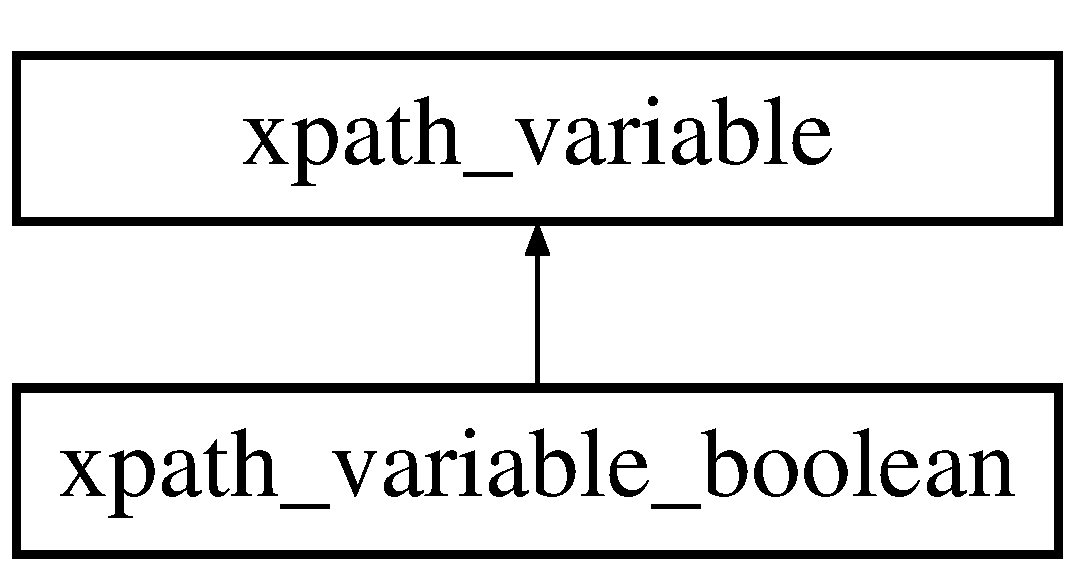
\includegraphics[height=2.000000cm]{structxpath__variable__boolean}
\end{center}
\end{figure}
\subsection*{Public Member Functions}
\begin{DoxyCompactItemize}
\item 
\hyperlink{structxpath__variable__boolean_a0d846c0137da3ceca54482939af4002c}{xpath\-\_\-variable\-\_\-boolean} ()
\end{DoxyCompactItemize}
\subsection*{Data Fields}
\begin{DoxyCompactItemize}
\item 
bool \hyperlink{structxpath__variable__boolean_ab54117a6cced8c3e029724651df4d404}{value}
\item 
char\-\_\-t \hyperlink{structxpath__variable__boolean_a2b2cb81ee5c9a19a667428d08d5bb951}{name} \mbox{[}1\mbox{]}
\end{DoxyCompactItemize}


\subsection{Constructor \& Destructor Documentation}
\hypertarget{structxpath__variable__boolean_a0d846c0137da3ceca54482939af4002c}{\index{xpath\-\_\-variable\-\_\-boolean@{xpath\-\_\-variable\-\_\-boolean}!xpath\-\_\-variable\-\_\-boolean@{xpath\-\_\-variable\-\_\-boolean}}
\index{xpath\-\_\-variable\-\_\-boolean@{xpath\-\_\-variable\-\_\-boolean}!xpath_variable_boolean@{xpath\-\_\-variable\-\_\-boolean}}
\subsubsection[{xpath\-\_\-variable\-\_\-boolean}]{\setlength{\rightskip}{0pt plus 5cm}xpath\-\_\-variable\-\_\-boolean\-::xpath\-\_\-variable\-\_\-boolean (
\begin{DoxyParamCaption}
{}
\end{DoxyParamCaption}
)\hspace{0.3cm}{\ttfamily [inline]}}}\label{structxpath__variable__boolean_a0d846c0137da3ceca54482939af4002c}

\begin{DoxyCode}
6606                                 : \hyperlink{structxpath__variable__boolean_ab54117a6cced8c3e029724651df4d404}{value}(\textcolor{keyword}{false})
6607         \{
6608         \}
\end{DoxyCode}


\subsection{Field Documentation}
\hypertarget{structxpath__variable__boolean_a2b2cb81ee5c9a19a667428d08d5bb951}{\index{xpath\-\_\-variable\-\_\-boolean@{xpath\-\_\-variable\-\_\-boolean}!name@{name}}
\index{name@{name}!xpath_variable_boolean@{xpath\-\_\-variable\-\_\-boolean}}
\subsubsection[{name}]{\setlength{\rightskip}{0pt plus 5cm}char\-\_\-t xpath\-\_\-variable\-\_\-boolean\-::name\mbox{[}1\mbox{]}}}\label{structxpath__variable__boolean_a2b2cb81ee5c9a19a667428d08d5bb951}
\hypertarget{structxpath__variable__boolean_ab54117a6cced8c3e029724651df4d404}{\index{xpath\-\_\-variable\-\_\-boolean@{xpath\-\_\-variable\-\_\-boolean}!value@{value}}
\index{value@{value}!xpath_variable_boolean@{xpath\-\_\-variable\-\_\-boolean}}
\subsubsection[{value}]{\setlength{\rightskip}{0pt plus 5cm}bool xpath\-\_\-variable\-\_\-boolean\-::value}}\label{structxpath__variable__boolean_ab54117a6cced8c3e029724651df4d404}


The documentation for this struct was generated from the following file\-:\begin{DoxyCompactItemize}
\item 
Third\-Party/pugixml/\hyperlink{pugixml_8cpp}{pugixml.\-cpp}\end{DoxyCompactItemize}

\hypertarget{structxpath__variable__node__set}{\section{xpath\-\_\-variable\-\_\-node\-\_\-set Struct Reference}
\label{structxpath__variable__node__set}\index{xpath\-\_\-variable\-\_\-node\-\_\-set@{xpath\-\_\-variable\-\_\-node\-\_\-set}}
}
Inheritance diagram for xpath\-\_\-variable\-\_\-node\-\_\-set\-:\begin{figure}[H]
\begin{center}
\leavevmode
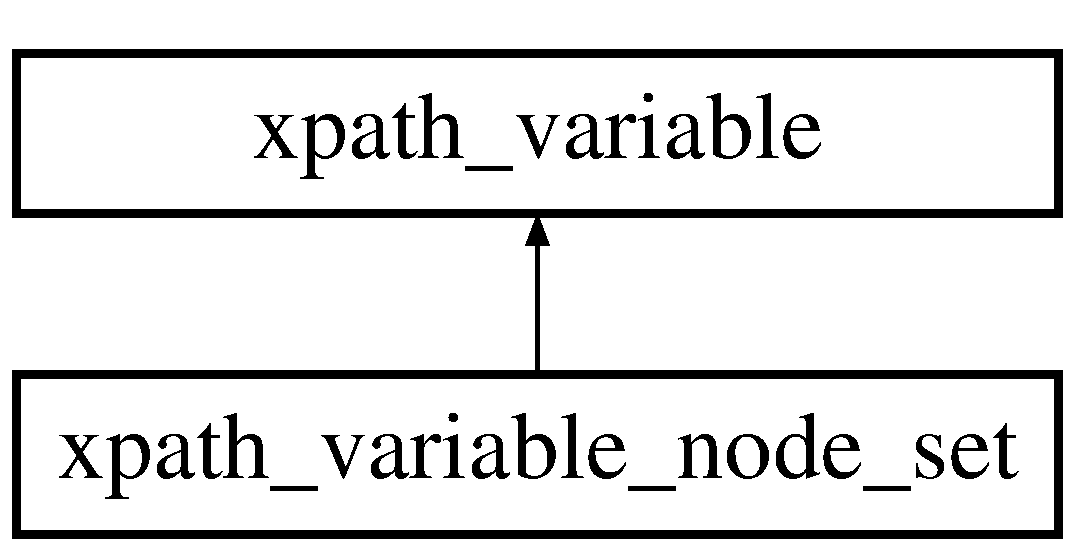
\includegraphics[height=2.000000cm]{structxpath__variable__node__set}
\end{center}
\end{figure}
\subsection*{Data Fields}
\begin{DoxyCompactItemize}
\item 
xpath\-\_\-node\-\_\-set \hyperlink{structxpath__variable__node__set_a830ac0dbcaf5f8ff3373d10273e72bf4}{value}
\item 
char\-\_\-t \hyperlink{structxpath__variable__node__set_a9a6a40cea40764364adb3ddba2e7a2ff}{name} \mbox{[}1\mbox{]}
\end{DoxyCompactItemize}


\subsection{Field Documentation}
\hypertarget{structxpath__variable__node__set_a9a6a40cea40764364adb3ddba2e7a2ff}{\index{xpath\-\_\-variable\-\_\-node\-\_\-set@{xpath\-\_\-variable\-\_\-node\-\_\-set}!name@{name}}
\index{name@{name}!xpath_variable_node_set@{xpath\-\_\-variable\-\_\-node\-\_\-set}}
\subsubsection[{name}]{\setlength{\rightskip}{0pt plus 5cm}char\-\_\-t xpath\-\_\-variable\-\_\-node\-\_\-set\-::name\mbox{[}1\mbox{]}}}\label{structxpath__variable__node__set_a9a6a40cea40764364adb3ddba2e7a2ff}
\hypertarget{structxpath__variable__node__set_a830ac0dbcaf5f8ff3373d10273e72bf4}{\index{xpath\-\_\-variable\-\_\-node\-\_\-set@{xpath\-\_\-variable\-\_\-node\-\_\-set}!value@{value}}
\index{value@{value}!xpath_variable_node_set@{xpath\-\_\-variable\-\_\-node\-\_\-set}}
\subsubsection[{value}]{\setlength{\rightskip}{0pt plus 5cm}xpath\-\_\-node\-\_\-set xpath\-\_\-variable\-\_\-node\-\_\-set\-::value}}\label{structxpath__variable__node__set_a830ac0dbcaf5f8ff3373d10273e72bf4}


The documentation for this struct was generated from the following file\-:\begin{DoxyCompactItemize}
\item 
Third\-Party/pugixml/\hyperlink{pugixml_8cpp}{pugixml.\-cpp}\end{DoxyCompactItemize}

\hypertarget{structxpath__variable__number}{\section{xpath\-\_\-variable\-\_\-number Struct Reference}
\label{structxpath__variable__number}\index{xpath\-\_\-variable\-\_\-number@{xpath\-\_\-variable\-\_\-number}}
}
Inheritance diagram for xpath\-\_\-variable\-\_\-number\-:\begin{figure}[H]
\begin{center}
\leavevmode
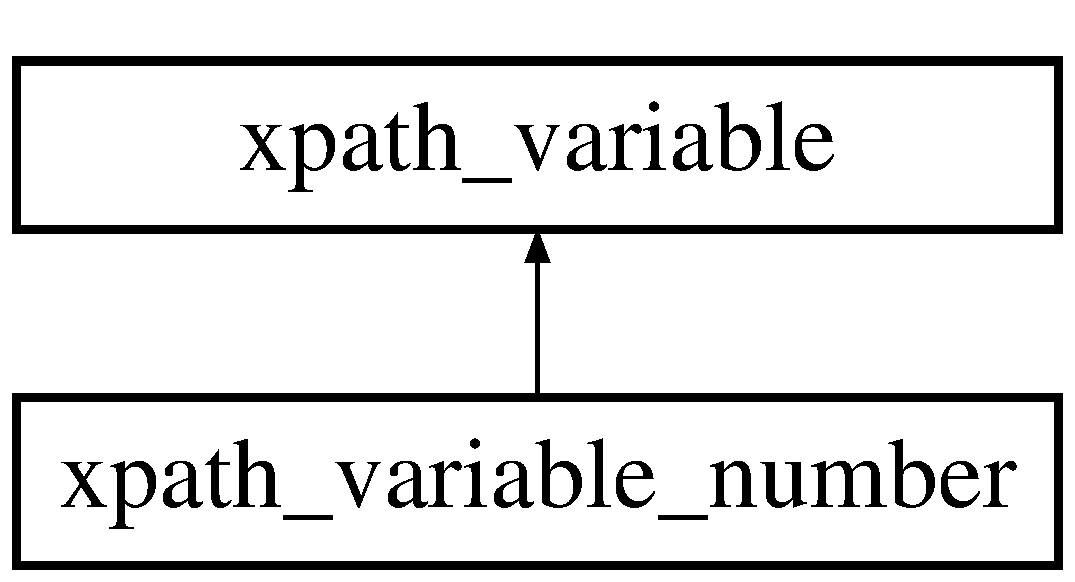
\includegraphics[height=2.000000cm]{structxpath__variable__number}
\end{center}
\end{figure}
\subsection*{Public Member Functions}
\begin{DoxyCompactItemize}
\item 
\hyperlink{structxpath__variable__number_ae139f6cc348a1ccb0d1fe97039a2d077}{xpath\-\_\-variable\-\_\-number} ()
\end{DoxyCompactItemize}
\subsection*{Data Fields}
\begin{DoxyCompactItemize}
\item 
double \hyperlink{structxpath__variable__number_a49949397348e7c941d88a694ec5c8e57}{value}
\item 
char\-\_\-t \hyperlink{structxpath__variable__number_a2bf4163dab1a8e233d45677fee987f0f}{name} \mbox{[}1\mbox{]}
\end{DoxyCompactItemize}


\subsection{Constructor \& Destructor Documentation}
\hypertarget{structxpath__variable__number_ae139f6cc348a1ccb0d1fe97039a2d077}{\index{xpath\-\_\-variable\-\_\-number@{xpath\-\_\-variable\-\_\-number}!xpath\-\_\-variable\-\_\-number@{xpath\-\_\-variable\-\_\-number}}
\index{xpath\-\_\-variable\-\_\-number@{xpath\-\_\-variable\-\_\-number}!xpath_variable_number@{xpath\-\_\-variable\-\_\-number}}
\subsubsection[{xpath\-\_\-variable\-\_\-number}]{\setlength{\rightskip}{0pt plus 5cm}xpath\-\_\-variable\-\_\-number\-::xpath\-\_\-variable\-\_\-number (
\begin{DoxyParamCaption}
{}
\end{DoxyParamCaption}
)\hspace{0.3cm}{\ttfamily [inline]}}}\label{structxpath__variable__number_ae139f6cc348a1ccb0d1fe97039a2d077}

\begin{DoxyCode}
6616                                : \hyperlink{structxpath__variable__number_a49949397348e7c941d88a694ec5c8e57}{value}(0)
6617         \{
6618         \}
\end{DoxyCode}


\subsection{Field Documentation}
\hypertarget{structxpath__variable__number_a2bf4163dab1a8e233d45677fee987f0f}{\index{xpath\-\_\-variable\-\_\-number@{xpath\-\_\-variable\-\_\-number}!name@{name}}
\index{name@{name}!xpath_variable_number@{xpath\-\_\-variable\-\_\-number}}
\subsubsection[{name}]{\setlength{\rightskip}{0pt plus 5cm}char\-\_\-t xpath\-\_\-variable\-\_\-number\-::name\mbox{[}1\mbox{]}}}\label{structxpath__variable__number_a2bf4163dab1a8e233d45677fee987f0f}
\hypertarget{structxpath__variable__number_a49949397348e7c941d88a694ec5c8e57}{\index{xpath\-\_\-variable\-\_\-number@{xpath\-\_\-variable\-\_\-number}!value@{value}}
\index{value@{value}!xpath_variable_number@{xpath\-\_\-variable\-\_\-number}}
\subsubsection[{value}]{\setlength{\rightskip}{0pt plus 5cm}double xpath\-\_\-variable\-\_\-number\-::value}}\label{structxpath__variable__number_a49949397348e7c941d88a694ec5c8e57}


The documentation for this struct was generated from the following file\-:\begin{DoxyCompactItemize}
\item 
Third\-Party/pugixml/\hyperlink{pugixml_8cpp}{pugixml.\-cpp}\end{DoxyCompactItemize}

\hypertarget{classpugi_1_1xpath__variable__set}{\section{pugi\-:\-:xpath\-\_\-variable\-\_\-set Class Reference}
\label{classpugi_1_1xpath__variable__set}\index{pugi\-::xpath\-\_\-variable\-\_\-set@{pugi\-::xpath\-\_\-variable\-\_\-set}}
}


{\ttfamily \#include $<$pugixml.\-hpp$>$}

\subsection*{Public Member Functions}
\begin{DoxyCompactItemize}
\item 
\hyperlink{classpugi_1_1xpath__variable__set_a7d5fcd43e16c9e8fe22cbfa10375789d}{xpath\-\_\-variable\-\_\-set} ()
\item 
\hyperlink{classpugi_1_1xpath__variable__set_a6a0df4fa59236eee33ba902691330f70}{$\sim$xpath\-\_\-variable\-\_\-set} ()
\item 
\hyperlink{classpugi_1_1xpath__variable}{xpath\-\_\-variable} $\ast$ \hyperlink{classpugi_1_1xpath__variable__set_a07051524f1c6a54bf8f16c9506d6ed5e}{add} (const \hyperlink{namespacepugi_aef5a7a62cba0507542220ea15afe39df}{char\-\_\-t} $\ast$name, \hyperlink{namespacepugi_ae3820874caf240e9f311bfd2790a84d6}{xpath\-\_\-value\-\_\-type} type)
\item 
bool \hyperlink{classpugi_1_1xpath__variable__set_a461660115640e623fe53af3d9f6b7a05}{set} (const \hyperlink{namespacepugi_aef5a7a62cba0507542220ea15afe39df}{char\-\_\-t} $\ast$name, bool value)
\item 
bool \hyperlink{classpugi_1_1xpath__variable__set_a74c45684cc9b790601830f5c51bb8b89}{set} (const \hyperlink{namespacepugi_aef5a7a62cba0507542220ea15afe39df}{char\-\_\-t} $\ast$name, double value)
\item 
bool \hyperlink{classpugi_1_1xpath__variable__set_a6c97731437c5aa4d57b72185ee03451c}{set} (const \hyperlink{namespacepugi_aef5a7a62cba0507542220ea15afe39df}{char\-\_\-t} $\ast$name, const \hyperlink{namespacepugi_aef5a7a62cba0507542220ea15afe39df}{char\-\_\-t} $\ast$value)
\item 
bool \hyperlink{classpugi_1_1xpath__variable__set_a5835902a2662631836cc6457709b84ec}{set} (const \hyperlink{namespacepugi_aef5a7a62cba0507542220ea15afe39df}{char\-\_\-t} $\ast$name, const \hyperlink{classpugi_1_1xpath__node__set}{xpath\-\_\-node\-\_\-set} \&value)
\item 
\hyperlink{classpugi_1_1xpath__variable}{xpath\-\_\-variable} $\ast$ \hyperlink{classpugi_1_1xpath__variable__set_aca5af5d65cdf0f639890cc1d3caec610}{get} (const \hyperlink{namespacepugi_aef5a7a62cba0507542220ea15afe39df}{char\-\_\-t} $\ast$name)
\item 
const \hyperlink{classpugi_1_1xpath__variable}{xpath\-\_\-variable} $\ast$ \hyperlink{classpugi_1_1xpath__variable__set_a6a15d76060162ae19f7c175af0c15cc3}{get} (const \hyperlink{namespacepugi_aef5a7a62cba0507542220ea15afe39df}{char\-\_\-t} $\ast$name) const 
\end{DoxyCompactItemize}


\subsection{Constructor \& Destructor Documentation}
\hypertarget{classpugi_1_1xpath__variable__set_a7d5fcd43e16c9e8fe22cbfa10375789d}{\index{pugi\-::xpath\-\_\-variable\-\_\-set@{pugi\-::xpath\-\_\-variable\-\_\-set}!xpath\-\_\-variable\-\_\-set@{xpath\-\_\-variable\-\_\-set}}
\index{xpath\-\_\-variable\-\_\-set@{xpath\-\_\-variable\-\_\-set}!pugi::xpath_variable_set@{pugi\-::xpath\-\_\-variable\-\_\-set}}
\subsubsection[{xpath\-\_\-variable\-\_\-set}]{\setlength{\rightskip}{0pt plus 5cm}{\bf P\-U\-G\-I\-\_\-\-\_\-\-F\-N} pugi\-::xpath\-\_\-variable\-\_\-set\-::xpath\-\_\-variable\-\_\-set (
\begin{DoxyParamCaption}
{}
\end{DoxyParamCaption}
)}}\label{classpugi_1_1xpath__variable__set_a7d5fcd43e16c9e8fe22cbfa10375789d}

\begin{DoxyCode}
9931     \{
9932         \textcolor{keywordflow}{for} (\textcolor{keywordtype}{size\_t} i = 0; i < \textcolor{keyword}{sizeof}(\_data) / \textcolor{keyword}{sizeof}(\_data[0]); ++i) \_data[i] = 0;
9933     \}
\end{DoxyCode}
\hypertarget{classpugi_1_1xpath__variable__set_a6a0df4fa59236eee33ba902691330f70}{\index{pugi\-::xpath\-\_\-variable\-\_\-set@{pugi\-::xpath\-\_\-variable\-\_\-set}!$\sim$xpath\-\_\-variable\-\_\-set@{$\sim$xpath\-\_\-variable\-\_\-set}}
\index{$\sim$xpath\-\_\-variable\-\_\-set@{$\sim$xpath\-\_\-variable\-\_\-set}!pugi::xpath_variable_set@{pugi\-::xpath\-\_\-variable\-\_\-set}}
\subsubsection[{$\sim$xpath\-\_\-variable\-\_\-set}]{\setlength{\rightskip}{0pt plus 5cm}{\bf P\-U\-G\-I\-\_\-\-\_\-\-F\-N} pugi\-::xpath\-\_\-variable\-\_\-set\-::$\sim$xpath\-\_\-variable\-\_\-set (
\begin{DoxyParamCaption}
{}
\end{DoxyParamCaption}
)}}\label{classpugi_1_1xpath__variable__set_a6a0df4fa59236eee33ba902691330f70}

\begin{DoxyCode}
9936     \{
9937         \textcolor{keywordflow}{for} (\textcolor{keywordtype}{size\_t} i = 0; i < \textcolor{keyword}{sizeof}(\_data) / \textcolor{keyword}{sizeof}(\_data[0]); ++i)
9938         \{
9939             xpath\_variable* var = \_data[i];
9940 
9941             \textcolor{keywordflow}{while} (var)
9942             \{
9943                 xpath\_variable* next = var->\hyperlink{classpugi_1_1xpath__variable_a0979cb72473e77a1b6d213046abfc46e}{\_next};
9944 
9945                 \hyperlink{pugixml_8cpp_aa9eac4e01f2efcc207d5c31cc308cad3}{impl::delete\_xpath\_variable}(var->\_type, var);
9946 
9947                 var = next;
9948             \}
9949         \}
9950     \}
\end{DoxyCode}


\subsection{Member Function Documentation}
\hypertarget{classpugi_1_1xpath__variable__set_a07051524f1c6a54bf8f16c9506d6ed5e}{\index{pugi\-::xpath\-\_\-variable\-\_\-set@{pugi\-::xpath\-\_\-variable\-\_\-set}!add@{add}}
\index{add@{add}!pugi::xpath_variable_set@{pugi\-::xpath\-\_\-variable\-\_\-set}}
\subsubsection[{add}]{\setlength{\rightskip}{0pt plus 5cm}{\bf P\-U\-G\-I\-\_\-\-\_\-\-F\-N} {\bf xpath\-\_\-variable} $\ast$ pugi\-::xpath\-\_\-variable\-\_\-set\-::add (
\begin{DoxyParamCaption}
\item[{const {\bf char\-\_\-t} $\ast$}]{name, }
\item[{{\bf xpath\-\_\-value\-\_\-type}}]{type}
\end{DoxyParamCaption}
)}}\label{classpugi_1_1xpath__variable__set_a07051524f1c6a54bf8f16c9506d6ed5e}

\begin{DoxyCode}
9966     \{
9967         \textcolor{keyword}{const} \textcolor{keywordtype}{size\_t} hash\_size = \textcolor{keyword}{sizeof}(\_data) / \textcolor{keyword}{sizeof}(\_data[0]);
9968         \textcolor{keywordtype}{size\_t} hash = \hyperlink{pugixml_8cpp_a2925a12bcdf39684733293ef195ae7e8}{impl::hash\_string}(name) % hash\_size;
9969 
9970         \textcolor{comment}{// look for existing variable}
9971         \textcolor{keywordflow}{for} (xpath\_variable* var = \_data[hash]; var; var = var->\_next)
9972             \textcolor{keywordflow}{if} (\hyperlink{pugixml_8cpp_af682718c79fea7fc666a593dc70764c1}{impl::strequal}(var->name(), name))
9973                 \textcolor{keywordflow}{return} var->type() == type ? var : 0;
9974 
9975         \textcolor{comment}{// add new variable}
9976         xpath\_variable* result = \hyperlink{pugixml_8cpp_a2ed6395c5799a328db6790347795af68}{impl::new\_xpath\_variable}(type, name);
9977 
9978         \textcolor{keywordflow}{if} (result)
9979         \{
9980             result->\_type = type;
9981             result->\_next = \_data[hash];
9982 
9983             \_data[hash] = result;
9984         \}
9985 
9986         \textcolor{keywordflow}{return} result;
9987     \}
\end{DoxyCode}
\hypertarget{classpugi_1_1xpath__variable__set_aca5af5d65cdf0f639890cc1d3caec610}{\index{pugi\-::xpath\-\_\-variable\-\_\-set@{pugi\-::xpath\-\_\-variable\-\_\-set}!get@{get}}
\index{get@{get}!pugi::xpath_variable_set@{pugi\-::xpath\-\_\-variable\-\_\-set}}
\subsubsection[{get}]{\setlength{\rightskip}{0pt plus 5cm}{\bf P\-U\-G\-I\-\_\-\-\_\-\-F\-N} {\bf xpath\-\_\-variable} $\ast$ pugi\-::xpath\-\_\-variable\-\_\-set\-::get (
\begin{DoxyParamCaption}
\item[{const {\bf char\-\_\-t} $\ast$}]{name}
\end{DoxyParamCaption}
)}}\label{classpugi_1_1xpath__variable__set_aca5af5d65cdf0f639890cc1d3caec610}

\begin{DoxyCode}
10014     \{
10015         \textcolor{keywordflow}{return} find(name);
10016     \}
\end{DoxyCode}
\hypertarget{classpugi_1_1xpath__variable__set_a6a15d76060162ae19f7c175af0c15cc3}{\index{pugi\-::xpath\-\_\-variable\-\_\-set@{pugi\-::xpath\-\_\-variable\-\_\-set}!get@{get}}
\index{get@{get}!pugi::xpath_variable_set@{pugi\-::xpath\-\_\-variable\-\_\-set}}
\subsubsection[{get}]{\setlength{\rightskip}{0pt plus 5cm}{\bf P\-U\-G\-I\-\_\-\-\_\-\-F\-N} const {\bf xpath\-\_\-variable} $\ast$ pugi\-::xpath\-\_\-variable\-\_\-set\-::get (
\begin{DoxyParamCaption}
\item[{const {\bf char\-\_\-t} $\ast$}]{name}
\end{DoxyParamCaption}
) const}}\label{classpugi_1_1xpath__variable__set_a6a15d76060162ae19f7c175af0c15cc3}

\begin{DoxyCode}
10019     \{
10020         \textcolor{keywordflow}{return} find(name);
10021     \}
\end{DoxyCode}
\hypertarget{classpugi_1_1xpath__variable__set_a461660115640e623fe53af3d9f6b7a05}{\index{pugi\-::xpath\-\_\-variable\-\_\-set@{pugi\-::xpath\-\_\-variable\-\_\-set}!set@{set}}
\index{set@{set}!pugi::xpath_variable_set@{pugi\-::xpath\-\_\-variable\-\_\-set}}
\subsubsection[{set}]{\setlength{\rightskip}{0pt plus 5cm}{\bf P\-U\-G\-I\-\_\-\-\_\-\-F\-N} bool pugi\-::xpath\-\_\-variable\-\_\-set\-::set (
\begin{DoxyParamCaption}
\item[{const {\bf char\-\_\-t} $\ast$}]{name, }
\item[{bool}]{value}
\end{DoxyParamCaption}
)}}\label{classpugi_1_1xpath__variable__set_a461660115640e623fe53af3d9f6b7a05}

\begin{DoxyCode}
9990     \{
9991         xpath\_variable* var = \hyperlink{classpugi_1_1xpath__variable__set_a07051524f1c6a54bf8f16c9506d6ed5e}{add}(name, \hyperlink{namespacepugi_ae3820874caf240e9f311bfd2790a84d6a049dd1494237a55f8aba3392d12a0164}{xpath\_type\_boolean});
9992         \textcolor{keywordflow}{return} var ? var->set(value) : \textcolor{keyword}{false};
9993     \}
\end{DoxyCode}
\hypertarget{classpugi_1_1xpath__variable__set_a74c45684cc9b790601830f5c51bb8b89}{\index{pugi\-::xpath\-\_\-variable\-\_\-set@{pugi\-::xpath\-\_\-variable\-\_\-set}!set@{set}}
\index{set@{set}!pugi::xpath_variable_set@{pugi\-::xpath\-\_\-variable\-\_\-set}}
\subsubsection[{set}]{\setlength{\rightskip}{0pt plus 5cm}{\bf P\-U\-G\-I\-\_\-\-\_\-\-F\-N} bool pugi\-::xpath\-\_\-variable\-\_\-set\-::set (
\begin{DoxyParamCaption}
\item[{const {\bf char\-\_\-t} $\ast$}]{name, }
\item[{double}]{value}
\end{DoxyParamCaption}
)}}\label{classpugi_1_1xpath__variable__set_a74c45684cc9b790601830f5c51bb8b89}

\begin{DoxyCode}
9996     \{
9997         xpath\_variable* var = \hyperlink{classpugi_1_1xpath__variable__set_a07051524f1c6a54bf8f16c9506d6ed5e}{add}(name, \hyperlink{namespacepugi_ae3820874caf240e9f311bfd2790a84d6a02959f74f4fe93d71a1e109a45f23825}{xpath\_type\_number});
9998         \textcolor{keywordflow}{return} var ? var->set(value) : \textcolor{keyword}{false};
9999     \}
\end{DoxyCode}
\hypertarget{classpugi_1_1xpath__variable__set_a6c97731437c5aa4d57b72185ee03451c}{\index{pugi\-::xpath\-\_\-variable\-\_\-set@{pugi\-::xpath\-\_\-variable\-\_\-set}!set@{set}}
\index{set@{set}!pugi::xpath_variable_set@{pugi\-::xpath\-\_\-variable\-\_\-set}}
\subsubsection[{set}]{\setlength{\rightskip}{0pt plus 5cm}{\bf P\-U\-G\-I\-\_\-\-\_\-\-F\-N} bool pugi\-::xpath\-\_\-variable\-\_\-set\-::set (
\begin{DoxyParamCaption}
\item[{const {\bf char\-\_\-t} $\ast$}]{name, }
\item[{const {\bf char\-\_\-t} $\ast$}]{value}
\end{DoxyParamCaption}
)}}\label{classpugi_1_1xpath__variable__set_a6c97731437c5aa4d57b72185ee03451c}

\begin{DoxyCode}
10002     \{
10003         xpath\_variable* var = \hyperlink{classpugi_1_1xpath__variable__set_a07051524f1c6a54bf8f16c9506d6ed5e}{add}(name, \hyperlink{namespacepugi_ae3820874caf240e9f311bfd2790a84d6ade2b17f4d9fad5bfb1617bf5012cf5ad}{xpath\_type\_string});
10004         \textcolor{keywordflow}{return} var ? var->set(value) : \textcolor{keyword}{false};
10005     \}
\end{DoxyCode}
\hypertarget{classpugi_1_1xpath__variable__set_a5835902a2662631836cc6457709b84ec}{\index{pugi\-::xpath\-\_\-variable\-\_\-set@{pugi\-::xpath\-\_\-variable\-\_\-set}!set@{set}}
\index{set@{set}!pugi::xpath_variable_set@{pugi\-::xpath\-\_\-variable\-\_\-set}}
\subsubsection[{set}]{\setlength{\rightskip}{0pt plus 5cm}{\bf P\-U\-G\-I\-\_\-\-\_\-\-F\-N} bool pugi\-::xpath\-\_\-variable\-\_\-set\-::set (
\begin{DoxyParamCaption}
\item[{const {\bf char\-\_\-t} $\ast$}]{name, }
\item[{const {\bf xpath\-\_\-node\-\_\-set} \&}]{value}
\end{DoxyParamCaption}
)}}\label{classpugi_1_1xpath__variable__set_a5835902a2662631836cc6457709b84ec}

\begin{DoxyCode}
10008     \{
10009         xpath\_variable* var = \hyperlink{classpugi_1_1xpath__variable__set_a07051524f1c6a54bf8f16c9506d6ed5e}{add}(name, \hyperlink{namespacepugi_ae3820874caf240e9f311bfd2790a84d6af5613748204e2e4861524e7d63a699c9}{xpath\_type\_node\_set});
10010         \textcolor{keywordflow}{return} var ? var->set(value) : \textcolor{keyword}{false};
10011     \}
\end{DoxyCode}


The documentation for this class was generated from the following files\-:\begin{DoxyCompactItemize}
\item 
Third\-Party/pugixml/\hyperlink{pugixml_8hpp}{pugixml.\-hpp}\item 
Third\-Party/pugixml/\hyperlink{pugixml_8cpp}{pugixml.\-cpp}\end{DoxyCompactItemize}

\hypertarget{structxpath__variable__string}{\section{xpath\-\_\-variable\-\_\-string Struct Reference}
\label{structxpath__variable__string}\index{xpath\-\_\-variable\-\_\-string@{xpath\-\_\-variable\-\_\-string}}
}
Inheritance diagram for xpath\-\_\-variable\-\_\-string\-:\begin{figure}[H]
\begin{center}
\leavevmode
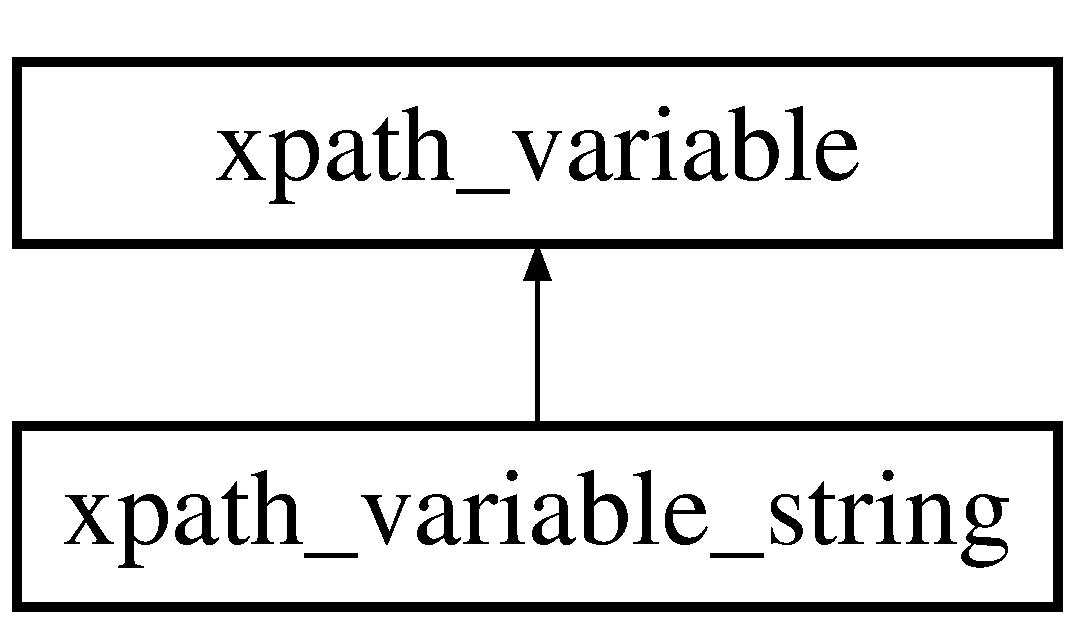
\includegraphics[height=2.000000cm]{structxpath__variable__string}
\end{center}
\end{figure}
\subsection*{Public Member Functions}
\begin{DoxyCompactItemize}
\item 
\hyperlink{structxpath__variable__string_a119d348b7f76371928faa5f5f80df815}{xpath\-\_\-variable\-\_\-string} ()
\item 
\hyperlink{structxpath__variable__string_a8e5e421f2e963e6196d2812a623ee912}{$\sim$xpath\-\_\-variable\-\_\-string} ()
\end{DoxyCompactItemize}
\subsection*{Data Fields}
\begin{DoxyCompactItemize}
\item 
char\-\_\-t $\ast$ \hyperlink{structxpath__variable__string_aeb8a87a8457d2615cd7b766fd3f30559}{value}
\item 
char\-\_\-t \hyperlink{structxpath__variable__string_a5c43cdcc55a620db0e7bdd29b4d56e89}{name} \mbox{[}1\mbox{]}
\end{DoxyCompactItemize}


\subsection{Constructor \& Destructor Documentation}
\hypertarget{structxpath__variable__string_a119d348b7f76371928faa5f5f80df815}{\index{xpath\-\_\-variable\-\_\-string@{xpath\-\_\-variable\-\_\-string}!xpath\-\_\-variable\-\_\-string@{xpath\-\_\-variable\-\_\-string}}
\index{xpath\-\_\-variable\-\_\-string@{xpath\-\_\-variable\-\_\-string}!xpath_variable_string@{xpath\-\_\-variable\-\_\-string}}
\subsubsection[{xpath\-\_\-variable\-\_\-string}]{\setlength{\rightskip}{0pt plus 5cm}xpath\-\_\-variable\-\_\-string\-::xpath\-\_\-variable\-\_\-string (
\begin{DoxyParamCaption}
{}
\end{DoxyParamCaption}
)\hspace{0.3cm}{\ttfamily [inline]}}}\label{structxpath__variable__string_a119d348b7f76371928faa5f5f80df815}

\begin{DoxyCode}
6626                                : \hyperlink{structxpath__variable__string_aeb8a87a8457d2615cd7b766fd3f30559}{value}(0)
6627         \{
6628         \}
\end{DoxyCode}
\hypertarget{structxpath__variable__string_a8e5e421f2e963e6196d2812a623ee912}{\index{xpath\-\_\-variable\-\_\-string@{xpath\-\_\-variable\-\_\-string}!$\sim$xpath\-\_\-variable\-\_\-string@{$\sim$xpath\-\_\-variable\-\_\-string}}
\index{$\sim$xpath\-\_\-variable\-\_\-string@{$\sim$xpath\-\_\-variable\-\_\-string}!xpath_variable_string@{xpath\-\_\-variable\-\_\-string}}
\subsubsection[{$\sim$xpath\-\_\-variable\-\_\-string}]{\setlength{\rightskip}{0pt plus 5cm}xpath\-\_\-variable\-\_\-string\-::$\sim$xpath\-\_\-variable\-\_\-string (
\begin{DoxyParamCaption}
{}
\end{DoxyParamCaption}
)\hspace{0.3cm}{\ttfamily [inline]}}}\label{structxpath__variable__string_a8e5e421f2e963e6196d2812a623ee912}

\begin{DoxyCode}
6631         \{
6632             \textcolor{keywordflow}{if} (\hyperlink{structxpath__variable__string_aeb8a87a8457d2615cd7b766fd3f30559}{value}) \hyperlink{structxml__memory__management__function__storage_a1c80a9a045ed6cfb90b17a178e4b3512}{xml\_memory::deallocate}(\hyperlink{structxpath__variable__string_aeb8a87a8457d2615cd7b766fd3f30559}{value});
6633         \}
\end{DoxyCode}


\subsection{Field Documentation}
\hypertarget{structxpath__variable__string_a5c43cdcc55a620db0e7bdd29b4d56e89}{\index{xpath\-\_\-variable\-\_\-string@{xpath\-\_\-variable\-\_\-string}!name@{name}}
\index{name@{name}!xpath_variable_string@{xpath\-\_\-variable\-\_\-string}}
\subsubsection[{name}]{\setlength{\rightskip}{0pt plus 5cm}char\-\_\-t xpath\-\_\-variable\-\_\-string\-::name\mbox{[}1\mbox{]}}}\label{structxpath__variable__string_a5c43cdcc55a620db0e7bdd29b4d56e89}
\hypertarget{structxpath__variable__string_aeb8a87a8457d2615cd7b766fd3f30559}{\index{xpath\-\_\-variable\-\_\-string@{xpath\-\_\-variable\-\_\-string}!value@{value}}
\index{value@{value}!xpath_variable_string@{xpath\-\_\-variable\-\_\-string}}
\subsubsection[{value}]{\setlength{\rightskip}{0pt plus 5cm}char\-\_\-t$\ast$ xpath\-\_\-variable\-\_\-string\-::value}}\label{structxpath__variable__string_aeb8a87a8457d2615cd7b766fd3f30559}


The documentation for this struct was generated from the following file\-:\begin{DoxyCompactItemize}
\item 
Third\-Party/pugixml/\hyperlink{pugixml_8cpp}{pugixml.\-cpp}\end{DoxyCompactItemize}

\chapter{File Documentation}
\hypertarget{controlcenter_8cpp}{\section{controlcenter.\-cpp File Reference}
\label{controlcenter_8cpp}\index{controlcenter.\-cpp@{controlcenter.\-cpp}}
}
{\ttfamily \#include \char`\"{}controlcenter.\-h\char`\"{}}\\*
{\ttfamily \#include \char`\"{}ui\-\_\-controlcenter.\-h\char`\"{}}\\*
{\ttfamily \#include $<$Q\-Shortcut$>$}\\*

\hypertarget{controlcenter_8h}{\section{controlcenter.\-h File Reference}
\label{controlcenter_8h}\index{controlcenter.\-h@{controlcenter.\-h}}
}
{\ttfamily \#include $<$list$>$}\\*
{\ttfamily \#include $<$Q\-Main\-Window$>$}\\*
{\ttfamily \#include \char`\"{}Types/camera.\-h\char`\"{}}\\*
{\ttfamily \#include \char`\"{}U\-I/videowindow.\-h\char`\"{}}\\*
{\ttfamily \#include \char`\"{}U\-I/icontrolcentermanager.\-h\char`\"{}}\\*
{\ttfamily \#include \char`\"{}Video/ffmpegwrapper.\-h\char`\"{}}\\*
{\ttfamily \#include \char`\"{}Learning\-Module/learninginterface.\-h\char`\"{}}\\*
{\ttfamily \#include $<$Q\-Thread$>$}\\*
\subsection*{Data Structures}
\begin{DoxyCompactItemize}
\item 
class \hyperlink{classControlCenter}{Control\-Center}
\begin{DoxyCompactList}\small\item\em This class defines the control center for the video client. \end{DoxyCompactList}\end{DoxyCompactItemize}
\subsection*{Namespaces}
\begin{DoxyCompactItemize}
\item 
\hyperlink{namespaceUi}{Ui}
\end{DoxyCompactItemize}

\hypertarget{Constants_8h}{\section{Global/\-Constants.h File Reference}
\label{Constants_8h}\index{Global/\-Constants.\-h@{Global/\-Constants.\-h}}
}
\subsection*{Macros}
\begin{DoxyCompactItemize}
\item 
\#define \hyperlink{Constants_8h_a456f72fbe9e6baf998125cfec71d6cfd}{L\-O\-G\-F\-I\-L\-E\-\_\-\-P\-A\-T\-H}~\char`\"{}logs/videostreamer.\-log\char`\"{}
\item 
\#define \hyperlink{Constants_8h_a5dcb1c9f587abfbe92034f35420f9ba4}{B\-W\-F\-I\-L\-E\-\_\-\-P\-A\-T\-H}~\char`\"{}/tmp/\char`\"{}
\item 
\#define \hyperlink{Constants_8h_ab4a334fc8f853017d86f4fd4db79b6de}{R\-E\-S\-O\-L\-U\-T\-I\-O\-N\-S\-\_\-\-F\-I\-L\-E}~\char`\"{}frame\-\_\-size\-\_\-options\char`\"{}
\item 
\#define \hyperlink{Constants_8h_aaaf30810788a2bf69f6391a7b8b1c541}{C\-A\-M\-E\-R\-A\-F\-I\-L\-E\-\_\-\-P\-A\-T\-H}~\char`\"{}Config/camera\-\_\-list\-\_\-example.\-xml\char`\"{}
\end{DoxyCompactItemize}


\subsection{Macro Definition Documentation}
\hypertarget{Constants_8h_a5dcb1c9f587abfbe92034f35420f9ba4}{\index{Constants.\-h@{Constants.\-h}!B\-W\-F\-I\-L\-E\-\_\-\-P\-A\-T\-H@{B\-W\-F\-I\-L\-E\-\_\-\-P\-A\-T\-H}}
\index{B\-W\-F\-I\-L\-E\-\_\-\-P\-A\-T\-H@{B\-W\-F\-I\-L\-E\-\_\-\-P\-A\-T\-H}!Constants.h@{Constants.\-h}}
\subsubsection[{B\-W\-F\-I\-L\-E\-\_\-\-P\-A\-T\-H}]{\setlength{\rightskip}{0pt plus 5cm}\#define B\-W\-F\-I\-L\-E\-\_\-\-P\-A\-T\-H~\char`\"{}/tmp/\char`\"{}}}\label{Constants_8h_a5dcb1c9f587abfbe92034f35420f9ba4}
\hypertarget{Constants_8h_aaaf30810788a2bf69f6391a7b8b1c541}{\index{Constants.\-h@{Constants.\-h}!C\-A\-M\-E\-R\-A\-F\-I\-L\-E\-\_\-\-P\-A\-T\-H@{C\-A\-M\-E\-R\-A\-F\-I\-L\-E\-\_\-\-P\-A\-T\-H}}
\index{C\-A\-M\-E\-R\-A\-F\-I\-L\-E\-\_\-\-P\-A\-T\-H@{C\-A\-M\-E\-R\-A\-F\-I\-L\-E\-\_\-\-P\-A\-T\-H}!Constants.h@{Constants.\-h}}
\subsubsection[{C\-A\-M\-E\-R\-A\-F\-I\-L\-E\-\_\-\-P\-A\-T\-H}]{\setlength{\rightskip}{0pt plus 5cm}\#define C\-A\-M\-E\-R\-A\-F\-I\-L\-E\-\_\-\-P\-A\-T\-H~\char`\"{}Config/camera\-\_\-list\-\_\-example.\-xml\char`\"{}}}\label{Constants_8h_aaaf30810788a2bf69f6391a7b8b1c541}
\hypertarget{Constants_8h_a456f72fbe9e6baf998125cfec71d6cfd}{\index{Constants.\-h@{Constants.\-h}!L\-O\-G\-F\-I\-L\-E\-\_\-\-P\-A\-T\-H@{L\-O\-G\-F\-I\-L\-E\-\_\-\-P\-A\-T\-H}}
\index{L\-O\-G\-F\-I\-L\-E\-\_\-\-P\-A\-T\-H@{L\-O\-G\-F\-I\-L\-E\-\_\-\-P\-A\-T\-H}!Constants.h@{Constants.\-h}}
\subsubsection[{L\-O\-G\-F\-I\-L\-E\-\_\-\-P\-A\-T\-H}]{\setlength{\rightskip}{0pt plus 5cm}\#define L\-O\-G\-F\-I\-L\-E\-\_\-\-P\-A\-T\-H~\char`\"{}logs/videostreamer.\-log\char`\"{}}}\label{Constants_8h_a456f72fbe9e6baf998125cfec71d6cfd}
\hypertarget{Constants_8h_ab4a334fc8f853017d86f4fd4db79b6de}{\index{Constants.\-h@{Constants.\-h}!R\-E\-S\-O\-L\-U\-T\-I\-O\-N\-S\-\_\-\-F\-I\-L\-E@{R\-E\-S\-O\-L\-U\-T\-I\-O\-N\-S\-\_\-\-F\-I\-L\-E}}
\index{R\-E\-S\-O\-L\-U\-T\-I\-O\-N\-S\-\_\-\-F\-I\-L\-E@{R\-E\-S\-O\-L\-U\-T\-I\-O\-N\-S\-\_\-\-F\-I\-L\-E}!Constants.h@{Constants.\-h}}
\subsubsection[{R\-E\-S\-O\-L\-U\-T\-I\-O\-N\-S\-\_\-\-F\-I\-L\-E}]{\setlength{\rightskip}{0pt plus 5cm}\#define R\-E\-S\-O\-L\-U\-T\-I\-O\-N\-S\-\_\-\-F\-I\-L\-E~\char`\"{}frame\-\_\-size\-\_\-options\char`\"{}}}\label{Constants_8h_ab4a334fc8f853017d86f4fd4db79b6de}

\hypertarget{Log_8h}{\section{Global/\-Log.h File Reference}
\label{Log_8h}\index{Global/\-Log.\-h@{Global/\-Log.\-h}}
}
{\ttfamily \#include \char`\"{}Qs\-Log.\-h\char`\"{}}\\*
\subsection*{Macros}
\begin{DoxyCompactItemize}
\item 
\#define \hyperlink{Log_8h_a9ade67d68c4294b0993315344532cf97}{F\-O\-R\-M\-A\-T}()~\-\_\-\-\_\-\-F\-I\-L\-E\-\_\-\-\_\- $<$$<$ \char`\"{}\-:\char`\"{} $<$$<$ \-\_\-\-\_\-\-L\-I\-N\-E\-\_\-\-\_\- $<$$<$ \char`\"{}-\/-\/\char`\"{}
\begin{DoxyCompactList}\small\item\em Define logging macros for custom formatting. \end{DoxyCompactList}\item 
\#define \hyperlink{Log_8h_a7d020b5dd8606c615fa96fbe2647a4b0}{T\-R\-A\-C\-E}()~Q\-L\-O\-G\-\_\-\-T\-R\-A\-C\-E() $<$$<$ \hyperlink{Log_8h_a9ade67d68c4294b0993315344532cf97}{F\-O\-R\-M\-A\-T}()
\begin{DoxyCompactList}\small\item\em Trace logging level. \end{DoxyCompactList}\item 
\#define \hyperlink{Log_8h_aba6772a53f37234ac4fa7570b4d49c5a}{D\-E\-B\-U\-G}()~Q\-L\-O\-G\-\_\-\-D\-E\-B\-U\-G() $<$$<$ \hyperlink{Log_8h_a9ade67d68c4294b0993315344532cf97}{F\-O\-R\-M\-A\-T}()
\begin{DoxyCompactList}\small\item\em Debug logging level. \end{DoxyCompactList}\item 
\#define \hyperlink{Log_8h_a7cec51f4ce4b22e8c0f256485d57fca7}{I\-N\-F\-O}()~Q\-L\-O\-G\-\_\-\-I\-N\-F\-O() $<$$<$ \hyperlink{Log_8h_a9ade67d68c4294b0993315344532cf97}{F\-O\-R\-M\-A\-T}()
\begin{DoxyCompactList}\small\item\em Info logging level. \end{DoxyCompactList}\item 
\#define \hyperlink{Log_8h_ad1ccc51e239005df4978895dae15497b}{W\-A\-R\-N}()~Q\-L\-O\-G\-\_\-\-W\-A\-R\-N() $<$$<$ \hyperlink{Log_8h_a9ade67d68c4294b0993315344532cf97}{F\-O\-R\-M\-A\-T}()
\begin{DoxyCompactList}\small\item\em Warning logging level. \end{DoxyCompactList}\item 
\#define \hyperlink{Log_8h_a1a242c34c5066fb0c62d909f22d3716d}{L\-\_\-\-E\-R\-R\-O\-R}()~Q\-L\-O\-G\-\_\-\-E\-R\-R\-O\-R() $<$$<$ \hyperlink{Log_8h_a9ade67d68c4294b0993315344532cf97}{F\-O\-R\-M\-A\-T}()
\begin{DoxyCompactList}\small\item\em Error logging level. \end{DoxyCompactList}\item 
\#define \hyperlink{Log_8h_a0134988ddb9f2cd0397f1ac985abd91c}{L\-O\-G\-\_\-\-P\-A\-T\-H}~\char`\"{}../logs/videostreamer.\-log\char`\"{}
\begin{DoxyCompactList}\small\item\em Define the log outfile. \end{DoxyCompactList}\end{DoxyCompactItemize}


\subsection{Macro Definition Documentation}
\hypertarget{Log_8h_aba6772a53f37234ac4fa7570b4d49c5a}{\index{Log.\-h@{Log.\-h}!D\-E\-B\-U\-G@{D\-E\-B\-U\-G}}
\index{D\-E\-B\-U\-G@{D\-E\-B\-U\-G}!Log.h@{Log.\-h}}
\subsubsection[{D\-E\-B\-U\-G}]{\setlength{\rightskip}{0pt plus 5cm}\#define D\-E\-B\-U\-G(
\begin{DoxyParamCaption}
{}
\end{DoxyParamCaption}
)~Q\-L\-O\-G\-\_\-\-D\-E\-B\-U\-G() $<$$<$ {\bf F\-O\-R\-M\-A\-T}()}}\label{Log_8h_aba6772a53f37234ac4fa7570b4d49c5a}


Debug logging level. 

\hypertarget{Log_8h_a9ade67d68c4294b0993315344532cf97}{\index{Log.\-h@{Log.\-h}!F\-O\-R\-M\-A\-T@{F\-O\-R\-M\-A\-T}}
\index{F\-O\-R\-M\-A\-T@{F\-O\-R\-M\-A\-T}!Log.h@{Log.\-h}}
\subsubsection[{F\-O\-R\-M\-A\-T}]{\setlength{\rightskip}{0pt plus 5cm}\#define F\-O\-R\-M\-A\-T(
\begin{DoxyParamCaption}
{}
\end{DoxyParamCaption}
)~\-\_\-\-\_\-\-F\-I\-L\-E\-\_\-\-\_\- $<$$<$ \char`\"{}\-:\char`\"{} $<$$<$ \-\_\-\-\_\-\-L\-I\-N\-E\-\_\-\-\_\- $<$$<$ \char`\"{}-\/-\/\char`\"{}}}\label{Log_8h_a9ade67d68c4294b0993315344532cf97}


Define logging macros for custom formatting. 

\hypertarget{Log_8h_a7cec51f4ce4b22e8c0f256485d57fca7}{\index{Log.\-h@{Log.\-h}!I\-N\-F\-O@{I\-N\-F\-O}}
\index{I\-N\-F\-O@{I\-N\-F\-O}!Log.h@{Log.\-h}}
\subsubsection[{I\-N\-F\-O}]{\setlength{\rightskip}{0pt plus 5cm}\#define I\-N\-F\-O(
\begin{DoxyParamCaption}
{}
\end{DoxyParamCaption}
)~Q\-L\-O\-G\-\_\-\-I\-N\-F\-O() $<$$<$ {\bf F\-O\-R\-M\-A\-T}()}}\label{Log_8h_a7cec51f4ce4b22e8c0f256485d57fca7}


Info logging level. 

\hypertarget{Log_8h_a1a242c34c5066fb0c62d909f22d3716d}{\index{Log.\-h@{Log.\-h}!L\-\_\-\-E\-R\-R\-O\-R@{L\-\_\-\-E\-R\-R\-O\-R}}
\index{L\-\_\-\-E\-R\-R\-O\-R@{L\-\_\-\-E\-R\-R\-O\-R}!Log.h@{Log.\-h}}
\subsubsection[{L\-\_\-\-E\-R\-R\-O\-R}]{\setlength{\rightskip}{0pt plus 5cm}\#define L\-\_\-\-E\-R\-R\-O\-R(
\begin{DoxyParamCaption}
{}
\end{DoxyParamCaption}
)~Q\-L\-O\-G\-\_\-\-E\-R\-R\-O\-R() $<$$<$ {\bf F\-O\-R\-M\-A\-T}()}}\label{Log_8h_a1a242c34c5066fb0c62d909f22d3716d}


Error logging level. 

\hypertarget{Log_8h_a0134988ddb9f2cd0397f1ac985abd91c}{\index{Log.\-h@{Log.\-h}!L\-O\-G\-\_\-\-P\-A\-T\-H@{L\-O\-G\-\_\-\-P\-A\-T\-H}}
\index{L\-O\-G\-\_\-\-P\-A\-T\-H@{L\-O\-G\-\_\-\-P\-A\-T\-H}!Log.h@{Log.\-h}}
\subsubsection[{L\-O\-G\-\_\-\-P\-A\-T\-H}]{\setlength{\rightskip}{0pt plus 5cm}\#define L\-O\-G\-\_\-\-P\-A\-T\-H~\char`\"{}../logs/videostreamer.\-log\char`\"{}}}\label{Log_8h_a0134988ddb9f2cd0397f1ac985abd91c}


Define the log outfile. 

\hypertarget{Log_8h_a7d020b5dd8606c615fa96fbe2647a4b0}{\index{Log.\-h@{Log.\-h}!T\-R\-A\-C\-E@{T\-R\-A\-C\-E}}
\index{T\-R\-A\-C\-E@{T\-R\-A\-C\-E}!Log.h@{Log.\-h}}
\subsubsection[{T\-R\-A\-C\-E}]{\setlength{\rightskip}{0pt plus 5cm}\#define T\-R\-A\-C\-E(
\begin{DoxyParamCaption}
{}
\end{DoxyParamCaption}
)~Q\-L\-O\-G\-\_\-\-T\-R\-A\-C\-E() $<$$<$ {\bf F\-O\-R\-M\-A\-T}()}}\label{Log_8h_a7d020b5dd8606c615fa96fbe2647a4b0}


Trace logging level. 

\hypertarget{Log_8h_ad1ccc51e239005df4978895dae15497b}{\index{Log.\-h@{Log.\-h}!W\-A\-R\-N@{W\-A\-R\-N}}
\index{W\-A\-R\-N@{W\-A\-R\-N}!Log.h@{Log.\-h}}
\subsubsection[{W\-A\-R\-N}]{\setlength{\rightskip}{0pt plus 5cm}\#define W\-A\-R\-N(
\begin{DoxyParamCaption}
{}
\end{DoxyParamCaption}
)~Q\-L\-O\-G\-\_\-\-W\-A\-R\-N() $<$$<$ {\bf F\-O\-R\-M\-A\-T}()}}\label{Log_8h_ad1ccc51e239005df4978895dae15497b}


Warning logging level. 


\hypertarget{SocketConstants_8h}{\section{Global/\-Socket\-Constants.h File Reference}
\label{SocketConstants_8h}\index{Global/\-Socket\-Constants.\-h@{Global/\-Socket\-Constants.\-h}}
}
\subsection*{Macros}
\begin{DoxyCompactItemize}
\item 
\#define \hyperlink{SocketConstants_8h_abcacfe0cacacfd5ec6a24b96e49715c3}{R\-E\-C\-E\-I\-V\-E\-R\-\_\-\-A\-D\-D\-R\-E\-S\-S}~\char`\"{}127.\-0.\-0.\-1\char`\"{}
\begin{DoxyCompactList}\small\item\em Receiver's address. \end{DoxyCompactList}\item 
\#define \hyperlink{SocketConstants_8h_a714d0c166e470fe1d95e17305a084931}{R\-E\-C\-E\-I\-V\-E\-R\-\_\-\-P\-O\-R\-T}~37986
\begin{DoxyCompactList}\small\item\em Receiver's listening port. \end{DoxyCompactList}\item 
\#define \hyperlink{SocketConstants_8h_a4fba0963c20988d1f1a45afb1c636e44}{L\-I\-S\-T\-E\-N\-\_\-\-P\-O\-R\-T}~7744
\begin{DoxyCompactList}\small\item\em Port we are listening for messages on. \end{DoxyCompactList}\item 
\#define \hyperlink{SocketConstants_8h_a92df38b61b193ac6bf60131babe08614}{S\-E\-N\-D\-\_\-\-P\-O\-R\-T}~7745
\begin{DoxyCompactList}\small\item\em Port we are sending messaged through. \end{DoxyCompactList}\item 
\#define \hyperlink{SocketConstants_8h_a12d15f06e320c26324ec45934324faf6}{S\-T\-R\-\_\-\-S\-E\-N\-D\-\_\-\-P\-O\-R\-T}~\char`\"{}7745\char`\"{}
\item 
\#define \hyperlink{SocketConstants_8h_aeefbbafa97642defe3ee6c3080b7d66f}{B\-A\-C\-K\-L\-O\-G}~2
\begin{DoxyCompactList}\small\item\em Backlog for incoming connections. \end{DoxyCompactList}\end{DoxyCompactItemize}


\subsection{Macro Definition Documentation}
\hypertarget{SocketConstants_8h_aeefbbafa97642defe3ee6c3080b7d66f}{\index{Socket\-Constants.\-h@{Socket\-Constants.\-h}!B\-A\-C\-K\-L\-O\-G@{B\-A\-C\-K\-L\-O\-G}}
\index{B\-A\-C\-K\-L\-O\-G@{B\-A\-C\-K\-L\-O\-G}!SocketConstants.h@{Socket\-Constants.\-h}}
\subsubsection[{B\-A\-C\-K\-L\-O\-G}]{\setlength{\rightskip}{0pt plus 5cm}\#define B\-A\-C\-K\-L\-O\-G~2}}\label{SocketConstants_8h_aeefbbafa97642defe3ee6c3080b7d66f}


Backlog for incoming connections. 

\hypertarget{SocketConstants_8h_a4fba0963c20988d1f1a45afb1c636e44}{\index{Socket\-Constants.\-h@{Socket\-Constants.\-h}!L\-I\-S\-T\-E\-N\-\_\-\-P\-O\-R\-T@{L\-I\-S\-T\-E\-N\-\_\-\-P\-O\-R\-T}}
\index{L\-I\-S\-T\-E\-N\-\_\-\-P\-O\-R\-T@{L\-I\-S\-T\-E\-N\-\_\-\-P\-O\-R\-T}!SocketConstants.h@{Socket\-Constants.\-h}}
\subsubsection[{L\-I\-S\-T\-E\-N\-\_\-\-P\-O\-R\-T}]{\setlength{\rightskip}{0pt plus 5cm}\#define L\-I\-S\-T\-E\-N\-\_\-\-P\-O\-R\-T~7744}}\label{SocketConstants_8h_a4fba0963c20988d1f1a45afb1c636e44}


Port we are listening for messages on. 

\hypertarget{SocketConstants_8h_abcacfe0cacacfd5ec6a24b96e49715c3}{\index{Socket\-Constants.\-h@{Socket\-Constants.\-h}!R\-E\-C\-E\-I\-V\-E\-R\-\_\-\-A\-D\-D\-R\-E\-S\-S@{R\-E\-C\-E\-I\-V\-E\-R\-\_\-\-A\-D\-D\-R\-E\-S\-S}}
\index{R\-E\-C\-E\-I\-V\-E\-R\-\_\-\-A\-D\-D\-R\-E\-S\-S@{R\-E\-C\-E\-I\-V\-E\-R\-\_\-\-A\-D\-D\-R\-E\-S\-S}!SocketConstants.h@{Socket\-Constants.\-h}}
\subsubsection[{R\-E\-C\-E\-I\-V\-E\-R\-\_\-\-A\-D\-D\-R\-E\-S\-S}]{\setlength{\rightskip}{0pt plus 5cm}\#define R\-E\-C\-E\-I\-V\-E\-R\-\_\-\-A\-D\-D\-R\-E\-S\-S~\char`\"{}127.\-0.\-0.\-1\char`\"{}}}\label{SocketConstants_8h_abcacfe0cacacfd5ec6a24b96e49715c3}


Receiver's address. 

\hypertarget{SocketConstants_8h_a714d0c166e470fe1d95e17305a084931}{\index{Socket\-Constants.\-h@{Socket\-Constants.\-h}!R\-E\-C\-E\-I\-V\-E\-R\-\_\-\-P\-O\-R\-T@{R\-E\-C\-E\-I\-V\-E\-R\-\_\-\-P\-O\-R\-T}}
\index{R\-E\-C\-E\-I\-V\-E\-R\-\_\-\-P\-O\-R\-T@{R\-E\-C\-E\-I\-V\-E\-R\-\_\-\-P\-O\-R\-T}!SocketConstants.h@{Socket\-Constants.\-h}}
\subsubsection[{R\-E\-C\-E\-I\-V\-E\-R\-\_\-\-P\-O\-R\-T}]{\setlength{\rightskip}{0pt plus 5cm}\#define R\-E\-C\-E\-I\-V\-E\-R\-\_\-\-P\-O\-R\-T~37986}}\label{SocketConstants_8h_a714d0c166e470fe1d95e17305a084931}


Receiver's listening port. 

\hypertarget{SocketConstants_8h_a92df38b61b193ac6bf60131babe08614}{\index{Socket\-Constants.\-h@{Socket\-Constants.\-h}!S\-E\-N\-D\-\_\-\-P\-O\-R\-T@{S\-E\-N\-D\-\_\-\-P\-O\-R\-T}}
\index{S\-E\-N\-D\-\_\-\-P\-O\-R\-T@{S\-E\-N\-D\-\_\-\-P\-O\-R\-T}!SocketConstants.h@{Socket\-Constants.\-h}}
\subsubsection[{S\-E\-N\-D\-\_\-\-P\-O\-R\-T}]{\setlength{\rightskip}{0pt plus 5cm}\#define S\-E\-N\-D\-\_\-\-P\-O\-R\-T~7745}}\label{SocketConstants_8h_a92df38b61b193ac6bf60131babe08614}


Port we are sending messaged through. 

\hypertarget{SocketConstants_8h_a12d15f06e320c26324ec45934324faf6}{\index{Socket\-Constants.\-h@{Socket\-Constants.\-h}!S\-T\-R\-\_\-\-S\-E\-N\-D\-\_\-\-P\-O\-R\-T@{S\-T\-R\-\_\-\-S\-E\-N\-D\-\_\-\-P\-O\-R\-T}}
\index{S\-T\-R\-\_\-\-S\-E\-N\-D\-\_\-\-P\-O\-R\-T@{S\-T\-R\-\_\-\-S\-E\-N\-D\-\_\-\-P\-O\-R\-T}!SocketConstants.h@{Socket\-Constants.\-h}}
\subsubsection[{S\-T\-R\-\_\-\-S\-E\-N\-D\-\_\-\-P\-O\-R\-T}]{\setlength{\rightskip}{0pt plus 5cm}\#define S\-T\-R\-\_\-\-S\-E\-N\-D\-\_\-\-P\-O\-R\-T~\char`\"{}7745\char`\"{}}}\label{SocketConstants_8h_a12d15f06e320c26324ec45934324faf6}

\hypertarget{SocketTypes_8h}{\section{Global/\-Socket\-Types.h File Reference}
\label{SocketTypes_8h}\index{Global/\-Socket\-Types.\-h@{Global/\-Socket\-Types.\-h}}
}
\subsection*{Typedefs}
\begin{DoxyCompactItemize}
\item 
typedef const char $\ast$ \hyperlink{SocketTypes_8h_a44dfeb3d24e205f47038cb0c772fec32}{S\-O\-C\-K\-\_\-\-T\-Y\-P\-E\-\_\-data\-\_\-buffer}
\begin{DoxyCompactList}\small\item\em Buffer type for packet data. \end{DoxyCompactList}\end{DoxyCompactItemize}


\subsection{Typedef Documentation}
\hypertarget{SocketTypes_8h_a44dfeb3d24e205f47038cb0c772fec32}{\index{Socket\-Types.\-h@{Socket\-Types.\-h}!S\-O\-C\-K\-\_\-\-T\-Y\-P\-E\-\_\-data\-\_\-buffer@{S\-O\-C\-K\-\_\-\-T\-Y\-P\-E\-\_\-data\-\_\-buffer}}
\index{S\-O\-C\-K\-\_\-\-T\-Y\-P\-E\-\_\-data\-\_\-buffer@{S\-O\-C\-K\-\_\-\-T\-Y\-P\-E\-\_\-data\-\_\-buffer}!SocketTypes.h@{Socket\-Types.\-h}}
\subsubsection[{S\-O\-C\-K\-\_\-\-T\-Y\-P\-E\-\_\-data\-\_\-buffer}]{\setlength{\rightskip}{0pt plus 5cm}typedef const char$\ast$ {\bf S\-O\-C\-K\-\_\-\-T\-Y\-P\-E\-\_\-data\-\_\-buffer}}}\label{SocketTypes_8h_a44dfeb3d24e205f47038cb0c772fec32}


Buffer type for packet data. 


\hypertarget{StdTypes_8h}{\section{Global/\-Std\-Types.h File Reference}
\label{StdTypes_8h}\index{Global/\-Std\-Types.\-h@{Global/\-Std\-Types.\-h}}
}
{\ttfamily \#include $<$list$>$}\\*
{\ttfamily \#include $<$string$>$}\\*
\subsection*{Namespaces}
\begin{DoxyCompactItemize}
\item 
\hyperlink{namespaceMainWindowUI}{Main\-Window\-U\-I}
\begin{DoxyCompactList}\small\item\em List typedefs for the older U\-I (not used anymore) \end{DoxyCompactList}\end{DoxyCompactItemize}
\subsection*{Typedefs}
\begin{DoxyCompactItemize}
\item 
typedef std\-::string \hyperlink{namespaceMainWindowUI_ab4a56a6d14c3fc1c53d1f1373a9033d3}{Main\-Window\-U\-I\-::\-Command\-List\-Item}
\item 
typedef std\-::list\\*
$<$ Command\-List\-Item $>$ \hyperlink{namespaceMainWindowUI_a746ebba19502abcb8ef74beecf9c6acf}{Main\-Window\-U\-I\-::\-Command\-List}
\item 
typedef std\-::list\\*
$<$ Command\-List\-Item $>$\-::iterator \hyperlink{namespaceMainWindowUI_acbc9d84cd79a821b6ff30f5ff94e9321}{Main\-Window\-U\-I\-::\-Command\-List\-Iterator}
\end{DoxyCompactItemize}

\hypertarget{logindialog_8cpp}{\section{logindialog.\-cpp File Reference}
\label{logindialog_8cpp}\index{logindialog.\-cpp@{logindialog.\-cpp}}
}
{\ttfamily \#include \char`\"{}logindialog.\-h\char`\"{}}\\*
{\ttfamily \#include \char`\"{}ui\-\_\-logindialog.\-h\char`\"{}}\\*
{\ttfamily \#include $<$Q\-Message\-Box$>$}\\*
{\ttfamily \#include \char`\"{}controlcenter.\-h\char`\"{}}\\*

\hypertarget{logindialog_8h}{\section{logindialog.\-h File Reference}
\label{logindialog_8h}\index{logindialog.\-h@{logindialog.\-h}}
}
{\ttfamily \#include $<$Q\-Dialog$>$}\\*
\subsection*{Data Structures}
\begin{DoxyCompactItemize}
\item 
class \hyperlink{classLoginDialog}{Login\-Dialog}
\end{DoxyCompactItemize}
\subsection*{Namespaces}
\begin{DoxyCompactItemize}
\item 
\hyperlink{namespaceUi}{Ui}
\end{DoxyCompactItemize}

\hypertarget{main_8cpp}{\section{main.\-cpp File Reference}
\label{main_8cpp}\index{main.\-cpp@{main.\-cpp}}
}
{\ttfamily \#include \char`\"{}Qs\-Log.\-h\char`\"{}}\\*
{\ttfamily \#include \char`\"{}Qs\-Log\-Dest.\-h\char`\"{}}\\*
{\ttfamily \#include \char`\"{}mainwindow.\-h\char`\"{}}\\*
{\ttfamily \#include \char`\"{}controlcenter.\-h\char`\"{}}\\*
{\ttfamily \#include \char`\"{}logindialog.\-h\char`\"{}}\\*
{\ttfamily \#include $<$Q\-Application$>$}\\*
{\ttfamily \#include $<$Q\-Dir$>$}\\*
\subsection*{Functions}
\begin{DoxyCompactItemize}
\item 
int \hyperlink{main_8cpp_a0ddf1224851353fc92bfbff6f499fa97}{main} (int argc, char $\ast$argv\mbox{[}$\,$\mbox{]})
\end{DoxyCompactItemize}


\subsection{Function Documentation}
\hypertarget{main_8cpp_a0ddf1224851353fc92bfbff6f499fa97}{\index{main.\-cpp@{main.\-cpp}!main@{main}}
\index{main@{main}!main.cpp@{main.\-cpp}}
\subsubsection[{main}]{\setlength{\rightskip}{0pt plus 5cm}int main (
\begin{DoxyParamCaption}
\item[{int}]{argc, }
\item[{char $\ast$}]{argv\mbox{[}$\,$\mbox{]}}
\end{DoxyParamCaption}
)}}\label{main_8cpp_a0ddf1224851353fc92bfbff6f499fa97}

\begin{DoxyCode}
10 \{
11     QApplication a(argc, argv);
12     \textcolor{comment}{//INITIALIZE LOGGER}
13     QsLogging::Logger& logger = QsLogging::Logger::instance();
14     logger.setLoggingLevel(QsLogging::DebugLevel);
15 
16     \textcolor{keyword}{const} QString path(QDir(a.applicationDirPath()).filePath(\textcolor{stringliteral}{"../logs/videostreamer.log"}));
17     QsLogging::DestinationPtr dest(QsLogging::DestinationFactory::MakeFileDestination(path));
18     logger.addDestination(dest.get());
19     QLOG\_INFO() << \_\_FILE\_\_ << \textcolor{stringliteral}{":"} << \_\_LINE\_\_ << \textcolor{stringliteral}{" -- "} << \textcolor{stringliteral}{"Program init."};
20     \textcolor{comment}{//MainWindow *w = new MainWindow;}
21     \textcolor{comment}{//w->show();}
22 \textcolor{comment}{//    ControlCenter *w = new ControlCenter;}
23 \textcolor{comment}{//    w->show();}
24     \hyperlink{classLoginDialog}{LoginDialog} *w = \textcolor{keyword}{new} \hyperlink{classLoginDialog}{LoginDialog};
25     w->show();
26 
27     \textcolor{keywordtype}{int} ret = a.exec();
28     \textcolor{keyword}{delete} w;
29     \textcolor{keywordflow}{return} ret;
30 \}
\end{DoxyCode}

\hypertarget{mainwindow_8cpp}{\section{mainwindow.\-cpp File Reference}
\label{mainwindow_8cpp}\index{mainwindow.\-cpp@{mainwindow.\-cpp}}
}
{\ttfamily \#include $<$Qt\-Global$>$}\\*
{\ttfamily \#include $<$Q\-Message\-Box$>$}\\*
{\ttfamily \#include $<$Q\-Progress\-Dialog$>$}\\*
{\ttfamily \#include $<$Q\-Progress\-Bar$>$}\\*
{\ttfamily \#include $<$Q\-Timer$>$}\\*
{\ttfamily \#include $<$exception$>$}\\*
{\ttfamily \#include $<$string$>$}\\*
{\ttfamily \#include \char`\"{}Global/\-Log.\-h\char`\"{}}\\*
{\ttfamily \#include \char`\"{}mainwindow.\-h\char`\"{}}\\*
{\ttfamily \#include \char`\"{}Global/\-Socket\-Types.\-h\char`\"{}}\\*
{\ttfamily \#include \char`\"{}ui\-\_\-mainwindow.\-h\char`\"{}}\\*
{\ttfamily \#include \char`\"{}Util/messagedispatcher.\-h\char`\"{}}\\*
{\ttfamily \#include \char`\"{}U\-I/videowindow.\-h\char`\"{}}\\*

\hypertarget{mainwindow_8h}{\section{mainwindow.\-h File Reference}
\label{mainwindow_8h}\index{mainwindow.\-h@{mainwindow.\-h}}
}
{\ttfamily \#include $<$Q\-Main\-Window$>$}\\*
{\ttfamily \#include $<$U\-I/serverpropertiesdialog.\-h$>$}\\*
{\ttfamily \#include $<$Q\-Thread$>$}\\*
{\ttfamily \#include $<$list$>$}\\*
{\ttfamily \#include \char`\"{}Network/networktoqtinterface.\-h\char`\"{}}\\*
{\ttfamily \#include \char`\"{}Network/address.\-h\char`\"{}}\\*
{\ttfamily \#include $<$U\-I/videowindow.\-h$>$}\\*
\subsection*{Data Structures}
\begin{DoxyCompactItemize}
\item 
class \hyperlink{classMainWindow}{Main\-Window}
\end{DoxyCompactItemize}
\subsection*{Namespaces}
\begin{DoxyCompactItemize}
\item 
\hyperlink{namespaceUi}{Ui}
\end{DoxyCompactItemize}

\hypertarget{address_8cpp}{\section{Network/address.cpp File Reference}
\label{address_8cpp}\index{Network/address.\-cpp@{Network/address.\-cpp}}
}
{\ttfamily \#include $<$strstream$>$}\\*
{\ttfamily \#include $<$string$>$}\\*
{\ttfamily \#include \char`\"{}Network/address.\-h\char`\"{}}\\*

\hypertarget{address_8h}{\section{Network/address.h File Reference}
\label{address_8h}\index{Network/address.\-h@{Network/address.\-h}}
}
{\ttfamily \#include $<$string$>$}\\*
\subsection*{Data Structures}
\begin{DoxyCompactItemize}
\item 
class \hyperlink{classAddress}{Address}
\begin{DoxyCompactList}\small\item\em \hyperlink{classAddress}{Address} type This class defines a type for a network address. \end{DoxyCompactList}\end{DoxyCompactItemize}

\hypertarget{networktoqtinterface_8cpp}{\section{Network/networktoqtinterface.cpp File Reference}
\label{networktoqtinterface_8cpp}\index{Network/networktoqtinterface.\-cpp@{Network/networktoqtinterface.\-cpp}}
}
{\ttfamily \#include $<$Q\-Application$>$}\\*
{\ttfamily \#include $<$Q\-Timer$>$}\\*
{\ttfamily \#include $<$Q\-Thread$>$}\\*
{\ttfamily \#include $<$Global/\-Log.\-h$>$}\\*
{\ttfamily \#include \char`\"{}networktoqtinterface.\-h\char`\"{}}\\*
{\ttfamily \#include \char`\"{}address.\-h\char`\"{}}\\*

\hypertarget{networktoqtinterface_8h}{\section{Network/networktoqtinterface.h File Reference}
\label{networktoqtinterface_8h}\index{Network/networktoqtinterface.\-h@{Network/networktoqtinterface.\-h}}
}
{\ttfamily \#include $<$Q\-Object$>$}\\*
{\ttfamily \#include $<$Util/tickingtimer.\-h$>$}\\*
{\ttfamily \#include \char`\"{}tcpclient.\-h\char`\"{}}\\*
{\ttfamily \#include \char`\"{}address.\-h\char`\"{}}\\*
\subsection*{Data Structures}
\begin{DoxyCompactItemize}
\item 
class \hyperlink{classNetworkToQtInterface}{Network\-To\-Qt\-Interface}
\begin{DoxyCompactList}\small\item\em The \hyperlink{classNetworkToQtInterface}{Network\-To\-Qt\-Interface} class. \end{DoxyCompactList}\end{DoxyCompactItemize}

\hypertarget{socket_8cpp}{\section{Network/socket.cpp File Reference}
\label{socket_8cpp}\index{Network/socket.\-cpp@{Network/socket.\-cpp}}
}
{\ttfamily \#include $<$Qt\-Global$>$}\\*
{\ttfamily \#include $<$errno.\-h$>$}\\*
{\ttfamily \#include \char`\"{}Global/\-Log.\-h\char`\"{}}\\*
{\ttfamily \#include \char`\"{}Network/socket.\-h\char`\"{}}\\*

\hypertarget{socket_8h}{\section{Network/socket.h File Reference}
\label{socket_8h}\index{Network/socket.\-h@{Network/socket.\-h}}
}
{\ttfamily \#include \char`\"{}Network/address.\-h\char`\"{}}\\*
\subsection*{Data Structures}
\begin{DoxyCompactItemize}
\item 
class \hyperlink{classSocket}{Socket}
\end{DoxyCompactItemize}

\hypertarget{tcpclient_8cpp}{\section{Network/tcpclient.cpp File Reference}
\label{tcpclient_8cpp}\index{Network/tcpclient.\-cpp@{Network/tcpclient.\-cpp}}
}
{\ttfamily \#include $<$Qt\-Global$>$}\\*
{\ttfamily \#include $<$errno.\-h$>$}\\*
{\ttfamily \#include $<$Global/\-Log.\-h$>$}\\*
{\ttfamily \#include $<$Global/\-Socket\-Constants.\-h$>$}\\*
{\ttfamily \#include $<$Network/address.\-h$>$}\\*
{\ttfamily \#include \char`\"{}tcpclient.\-h\char`\"{}}\\*

\hypertarget{tcpclient_8h}{\section{Network/tcpclient.h File Reference}
\label{tcpclient_8h}\index{Network/tcpclient.\-h@{Network/tcpclient.\-h}}
}
\subsection*{Data Structures}
\begin{DoxyCompactItemize}
\item 
class \hyperlink{classTCPClient}{T\-C\-P\-Client}
\begin{DoxyCompactList}\small\item\em This class defines a T\-C\-P client that will send requests to and receive responses from a specified server. \end{DoxyCompactList}\end{DoxyCompactItemize}
\subsection*{Enumerations}
\begin{DoxyCompactItemize}
\item 
enum \hyperlink{tcpclient_8h_ab36b81f0daebbad95a533ea9951ee569}{T\-C\-P\-Error} \{ \\*
\hyperlink{tcpclient_8h_ab36b81f0daebbad95a533ea9951ee569a12de2815c3e64df634ac4d26a0bb2007}{T\-C\-P\-\_\-\-S\-T\-A\-T\-U\-S\-\_\-\-S\-U\-C\-C\-E\-S\-S} = 0, 
\hyperlink{tcpclient_8h_ab36b81f0daebbad95a533ea9951ee569a677e05a70195600d99f343ac4d080f12}{T\-C\-P\-\_\-\-S\-T\-A\-T\-U\-S\-\_\-\-A\-D\-D\-R\-E\-S\-S\-\_\-\-N\-O\-T\-\_\-\-F\-O\-U\-N\-D} = 1, 
\hyperlink{tcpclient_8h_ab36b81f0daebbad95a533ea9951ee569afbc7ac61946e52ae324b1c658cf45e3a}{T\-C\-P\-\_\-\-S\-T\-A\-T\-U\-S\-\_\-\-S\-O\-C\-K\-E\-T\-\_\-\-N\-O\-T\-\_\-\-O\-P\-E\-N\-E\-D} = 2, 
\hyperlink{tcpclient_8h_ab36b81f0daebbad95a533ea9951ee569a31579e5845f194f359afdb50b2f85a86}{T\-C\-P\-\_\-\-S\-T\-A\-T\-U\-S\-\_\-\-C\-O\-N\-N\-E\-C\-T\-I\-O\-N\-\_\-\-C\-L\-O\-S\-E\-D} = 3, 
\\*
\hyperlink{tcpclient_8h_ab36b81f0daebbad95a533ea9951ee569a0fbe81dbe6a6972d6c80cecad3ee0d73}{T\-C\-P\-\_\-\-S\-T\-A\-T\-U\-S\-\_\-\-S\-E\-N\-D\-\_\-\-F\-A\-I\-L\-E\-D} = 4, 
\hyperlink{tcpclient_8h_ab36b81f0daebbad95a533ea9951ee569a9b5153de6f52108f95fe6f5ccec7e05d}{T\-C\-P\-\_\-\-S\-T\-A\-T\-U\-S\-\_\-\-R\-E\-C\-E\-I\-V\-E\-\_\-\-F\-A\-I\-L\-E\-D} = 5, 
\hyperlink{tcpclient_8h_ab36b81f0daebbad95a533ea9951ee569a1f2b9b8cedc20d11900f30d9df9c8b1f}{T\-C\-P\-\_\-\-S\-T\-A\-T\-U\-S\-\_\-\-S\-E\-R\-V\-E\-R\-\_\-\-D\-I\-S\-C\-O\-N\-N\-E\-C\-T\-E\-D} = 6
 \}
\begin{DoxyCompactList}\small\item\em Enumeration for the T\-C\-P\-Error type. \end{DoxyCompactList}\end{DoxyCompactItemize}


\subsection{Enumeration Type Documentation}
\hypertarget{tcpclient_8h_ab36b81f0daebbad95a533ea9951ee569}{\index{tcpclient.\-h@{tcpclient.\-h}!T\-C\-P\-Error@{T\-C\-P\-Error}}
\index{T\-C\-P\-Error@{T\-C\-P\-Error}!tcpclient.h@{tcpclient.\-h}}
\subsubsection[{T\-C\-P\-Error}]{\setlength{\rightskip}{0pt plus 5cm}enum {\bf T\-C\-P\-Error}}}\label{tcpclient_8h_ab36b81f0daebbad95a533ea9951ee569}


Enumeration for the T\-C\-P\-Error type. 

\begin{Desc}
\item[Enumerator]\par
\begin{description}
\index{T\-C\-P\-\_\-\-S\-T\-A\-T\-U\-S\-\_\-\-S\-U\-C\-C\-E\-S\-S@{T\-C\-P\-\_\-\-S\-T\-A\-T\-U\-S\-\_\-\-S\-U\-C\-C\-E\-S\-S}!tcpclient.\-h@{tcpclient.\-h}}\index{tcpclient.\-h@{tcpclient.\-h}!T\-C\-P\-\_\-\-S\-T\-A\-T\-U\-S\-\_\-\-S\-U\-C\-C\-E\-S\-S@{T\-C\-P\-\_\-\-S\-T\-A\-T\-U\-S\-\_\-\-S\-U\-C\-C\-E\-S\-S}}\item[{\em 
\hypertarget{tcpclient_8h_ab36b81f0daebbad95a533ea9951ee569a12de2815c3e64df634ac4d26a0bb2007}{T\-C\-P\-\_\-\-S\-T\-A\-T\-U\-S\-\_\-\-S\-U\-C\-C\-E\-S\-S}\label{tcpclient_8h_ab36b81f0daebbad95a533ea9951ee569a12de2815c3e64df634ac4d26a0bb2007}
}]No errors. \index{T\-C\-P\-\_\-\-S\-T\-A\-T\-U\-S\-\_\-\-A\-D\-D\-R\-E\-S\-S\-\_\-\-N\-O\-T\-\_\-\-F\-O\-U\-N\-D@{T\-C\-P\-\_\-\-S\-T\-A\-T\-U\-S\-\_\-\-A\-D\-D\-R\-E\-S\-S\-\_\-\-N\-O\-T\-\_\-\-F\-O\-U\-N\-D}!tcpclient.\-h@{tcpclient.\-h}}\index{tcpclient.\-h@{tcpclient.\-h}!T\-C\-P\-\_\-\-S\-T\-A\-T\-U\-S\-\_\-\-A\-D\-D\-R\-E\-S\-S\-\_\-\-N\-O\-T\-\_\-\-F\-O\-U\-N\-D@{T\-C\-P\-\_\-\-S\-T\-A\-T\-U\-S\-\_\-\-A\-D\-D\-R\-E\-S\-S\-\_\-\-N\-O\-T\-\_\-\-F\-O\-U\-N\-D}}\item[{\em 
\hypertarget{tcpclient_8h_ab36b81f0daebbad95a533ea9951ee569a677e05a70195600d99f343ac4d080f12}{T\-C\-P\-\_\-\-S\-T\-A\-T\-U\-S\-\_\-\-A\-D\-D\-R\-E\-S\-S\-\_\-\-N\-O\-T\-\_\-\-F\-O\-U\-N\-D}\label{tcpclient_8h_ab36b81f0daebbad95a533ea9951ee569a677e05a70195600d99f343ac4d080f12}
}]Could not find the specified server. \index{T\-C\-P\-\_\-\-S\-T\-A\-T\-U\-S\-\_\-\-S\-O\-C\-K\-E\-T\-\_\-\-N\-O\-T\-\_\-\-O\-P\-E\-N\-E\-D@{T\-C\-P\-\_\-\-S\-T\-A\-T\-U\-S\-\_\-\-S\-O\-C\-K\-E\-T\-\_\-\-N\-O\-T\-\_\-\-O\-P\-E\-N\-E\-D}!tcpclient.\-h@{tcpclient.\-h}}\index{tcpclient.\-h@{tcpclient.\-h}!T\-C\-P\-\_\-\-S\-T\-A\-T\-U\-S\-\_\-\-S\-O\-C\-K\-E\-T\-\_\-\-N\-O\-T\-\_\-\-O\-P\-E\-N\-E\-D@{T\-C\-P\-\_\-\-S\-T\-A\-T\-U\-S\-\_\-\-S\-O\-C\-K\-E\-T\-\_\-\-N\-O\-T\-\_\-\-O\-P\-E\-N\-E\-D}}\item[{\em 
\hypertarget{tcpclient_8h_ab36b81f0daebbad95a533ea9951ee569afbc7ac61946e52ae324b1c658cf45e3a}{T\-C\-P\-\_\-\-S\-T\-A\-T\-U\-S\-\_\-\-S\-O\-C\-K\-E\-T\-\_\-\-N\-O\-T\-\_\-\-O\-P\-E\-N\-E\-D}\label{tcpclient_8h_ab36b81f0daebbad95a533ea9951ee569afbc7ac61946e52ae324b1c658cf45e3a}
}]Could not open a socket. \index{T\-C\-P\-\_\-\-S\-T\-A\-T\-U\-S\-\_\-\-C\-O\-N\-N\-E\-C\-T\-I\-O\-N\-\_\-\-C\-L\-O\-S\-E\-D@{T\-C\-P\-\_\-\-S\-T\-A\-T\-U\-S\-\_\-\-C\-O\-N\-N\-E\-C\-T\-I\-O\-N\-\_\-\-C\-L\-O\-S\-E\-D}!tcpclient.\-h@{tcpclient.\-h}}\index{tcpclient.\-h@{tcpclient.\-h}!T\-C\-P\-\_\-\-S\-T\-A\-T\-U\-S\-\_\-\-C\-O\-N\-N\-E\-C\-T\-I\-O\-N\-\_\-\-C\-L\-O\-S\-E\-D@{T\-C\-P\-\_\-\-S\-T\-A\-T\-U\-S\-\_\-\-C\-O\-N\-N\-E\-C\-T\-I\-O\-N\-\_\-\-C\-L\-O\-S\-E\-D}}\item[{\em 
\hypertarget{tcpclient_8h_ab36b81f0daebbad95a533ea9951ee569a31579e5845f194f359afdb50b2f85a86}{T\-C\-P\-\_\-\-S\-T\-A\-T\-U\-S\-\_\-\-C\-O\-N\-N\-E\-C\-T\-I\-O\-N\-\_\-\-C\-L\-O\-S\-E\-D}\label{tcpclient_8h_ab36b81f0daebbad95a533ea9951ee569a31579e5845f194f359afdb50b2f85a86}
}]Conection lost. \index{T\-C\-P\-\_\-\-S\-T\-A\-T\-U\-S\-\_\-\-S\-E\-N\-D\-\_\-\-F\-A\-I\-L\-E\-D@{T\-C\-P\-\_\-\-S\-T\-A\-T\-U\-S\-\_\-\-S\-E\-N\-D\-\_\-\-F\-A\-I\-L\-E\-D}!tcpclient.\-h@{tcpclient.\-h}}\index{tcpclient.\-h@{tcpclient.\-h}!T\-C\-P\-\_\-\-S\-T\-A\-T\-U\-S\-\_\-\-S\-E\-N\-D\-\_\-\-F\-A\-I\-L\-E\-D@{T\-C\-P\-\_\-\-S\-T\-A\-T\-U\-S\-\_\-\-S\-E\-N\-D\-\_\-\-F\-A\-I\-L\-E\-D}}\item[{\em 
\hypertarget{tcpclient_8h_ab36b81f0daebbad95a533ea9951ee569a0fbe81dbe6a6972d6c80cecad3ee0d73}{T\-C\-P\-\_\-\-S\-T\-A\-T\-U\-S\-\_\-\-S\-E\-N\-D\-\_\-\-F\-A\-I\-L\-E\-D}\label{tcpclient_8h_ab36b81f0daebbad95a533ea9951ee569a0fbe81dbe6a6972d6c80cecad3ee0d73}
}]Failed to send a request. \index{T\-C\-P\-\_\-\-S\-T\-A\-T\-U\-S\-\_\-\-R\-E\-C\-E\-I\-V\-E\-\_\-\-F\-A\-I\-L\-E\-D@{T\-C\-P\-\_\-\-S\-T\-A\-T\-U\-S\-\_\-\-R\-E\-C\-E\-I\-V\-E\-\_\-\-F\-A\-I\-L\-E\-D}!tcpclient.\-h@{tcpclient.\-h}}\index{tcpclient.\-h@{tcpclient.\-h}!T\-C\-P\-\_\-\-S\-T\-A\-T\-U\-S\-\_\-\-R\-E\-C\-E\-I\-V\-E\-\_\-\-F\-A\-I\-L\-E\-D@{T\-C\-P\-\_\-\-S\-T\-A\-T\-U\-S\-\_\-\-R\-E\-C\-E\-I\-V\-E\-\_\-\-F\-A\-I\-L\-E\-D}}\item[{\em 
\hypertarget{tcpclient_8h_ab36b81f0daebbad95a533ea9951ee569a9b5153de6f52108f95fe6f5ccec7e05d}{T\-C\-P\-\_\-\-S\-T\-A\-T\-U\-S\-\_\-\-R\-E\-C\-E\-I\-V\-E\-\_\-\-F\-A\-I\-L\-E\-D}\label{tcpclient_8h_ab36b81f0daebbad95a533ea9951ee569a9b5153de6f52108f95fe6f5ccec7e05d}
}]Failed to receive a response. \index{T\-C\-P\-\_\-\-S\-T\-A\-T\-U\-S\-\_\-\-S\-E\-R\-V\-E\-R\-\_\-\-D\-I\-S\-C\-O\-N\-N\-E\-C\-T\-E\-D@{T\-C\-P\-\_\-\-S\-T\-A\-T\-U\-S\-\_\-\-S\-E\-R\-V\-E\-R\-\_\-\-D\-I\-S\-C\-O\-N\-N\-E\-C\-T\-E\-D}!tcpclient.\-h@{tcpclient.\-h}}\index{tcpclient.\-h@{tcpclient.\-h}!T\-C\-P\-\_\-\-S\-T\-A\-T\-U\-S\-\_\-\-S\-E\-R\-V\-E\-R\-\_\-\-D\-I\-S\-C\-O\-N\-N\-E\-C\-T\-E\-D@{T\-C\-P\-\_\-\-S\-T\-A\-T\-U\-S\-\_\-\-S\-E\-R\-V\-E\-R\-\_\-\-D\-I\-S\-C\-O\-N\-N\-E\-C\-T\-E\-D}}\item[{\em 
\hypertarget{tcpclient_8h_ab36b81f0daebbad95a533ea9951ee569a1f2b9b8cedc20d11900f30d9df9c8b1f}{T\-C\-P\-\_\-\-S\-T\-A\-T\-U\-S\-\_\-\-S\-E\-R\-V\-E\-R\-\_\-\-D\-I\-S\-C\-O\-N\-N\-E\-C\-T\-E\-D}\label{tcpclient_8h_ab36b81f0daebbad95a533ea9951ee569a1f2b9b8cedc20d11900f30d9df9c8b1f}
}]Server disconnected. \end{description}
\end{Desc}

\begin{DoxyCode}
10 \{
11     \hyperlink{tcpclient_8h_ab36b81f0daebbad95a533ea9951ee569a12de2815c3e64df634ac4d26a0bb2007}{TCP\_STATUS\_SUCCESS} = 0,                 
12     \hyperlink{tcpclient_8h_ab36b81f0daebbad95a533ea9951ee569a677e05a70195600d99f343ac4d080f12}{TCP\_STATUS\_ADDRESS\_NOT\_FOUND} = 1,       
13     \hyperlink{tcpclient_8h_ab36b81f0daebbad95a533ea9951ee569afbc7ac61946e52ae324b1c658cf45e3a}{TCP\_STATUS\_SOCKET\_NOT\_OPENED} = 2,       
14     \hyperlink{tcpclient_8h_ab36b81f0daebbad95a533ea9951ee569a31579e5845f194f359afdb50b2f85a86}{TCP\_STATUS\_CONNECTION\_CLOSED} = 3,       
15     \hyperlink{tcpclient_8h_ab36b81f0daebbad95a533ea9951ee569a0fbe81dbe6a6972d6c80cecad3ee0d73}{TCP\_STATUS\_SEND\_FAILED} = 4,             
16     \hyperlink{tcpclient_8h_ab36b81f0daebbad95a533ea9951ee569a9b5153de6f52108f95fe6f5ccec7e05d}{TCP\_STATUS\_RECEIVE\_FAILED} = 5,          
17     \hyperlink{tcpclient_8h_ab36b81f0daebbad95a533ea9951ee569a1f2b9b8cedc20d11900f30d9df9c8b1f}{TCP\_STATUS\_SERVER\_DISCONNECTED} = 6      
18 \};
\end{DoxyCode}

\hypertarget{pugiconfig_8hpp}{\section{Third\-Party/pugixml/pugiconfig.hpp File Reference}
\label{pugiconfig_8hpp}\index{Third\-Party/pugixml/pugiconfig.\-hpp@{Third\-Party/pugixml/pugiconfig.\-hpp}}
}

\hypertarget{pugixml_8cpp}{\section{Third\-Party/pugixml/pugixml.cpp File Reference}
\label{pugixml_8cpp}\index{Third\-Party/pugixml/pugixml.\-cpp@{Third\-Party/pugixml/pugixml.\-cpp}}
}
{\ttfamily \#include \char`\"{}pugixml.\-hpp\char`\"{}}\\*
{\ttfamily \#include $<$stdlib.\-h$>$}\\*
{\ttfamily \#include $<$stdio.\-h$>$}\\*
{\ttfamily \#include $<$string.\-h$>$}\\*
{\ttfamily \#include $<$assert.\-h$>$}\\*
{\ttfamily \#include $<$wchar.\-h$>$}\\*
{\ttfamily \#include $<$math.\-h$>$}\\*
{\ttfamily \#include $<$float.\-h$>$}\\*
{\ttfamily \#include $<$istream$>$}\\*
{\ttfamily \#include $<$ostream$>$}\\*
{\ttfamily \#include $<$string$>$}\\*
{\ttfamily \#include $<$new$>$}\\*
{\ttfamily \#include $<$stdint.\-h$>$}\\*
\subsection*{Data Structures}
\begin{DoxyCompactItemize}
\item 
struct \hyperlink{structxml__memory__management__function__storage}{xml\-\_\-memory\-\_\-management\-\_\-function\-\_\-storage$<$ T $>$}
\item 
struct \hyperlink{structbuffer__holder}{buffer\-\_\-holder}
\item 
struct \hyperlink{structxml__memory__page}{xml\-\_\-memory\-\_\-page}
\item 
struct \hyperlink{structxml__memory__string__header}{xml\-\_\-memory\-\_\-string\-\_\-header}
\item 
struct \hyperlink{structxml__allocator}{xml\-\_\-allocator}
\item 
struct \hyperlink{structpugi_1_1xml__attribute__struct}{pugi\-::xml\-\_\-attribute\-\_\-struct}
\begin{DoxyCompactList}\small\item\em A 'name=value' X\-M\-L attribute structure. \end{DoxyCompactList}\item 
struct \hyperlink{structpugi_1_1xml__node__struct}{pugi\-::xml\-\_\-node\-\_\-struct}
\begin{DoxyCompactList}\small\item\em An X\-M\-L document tree node. \end{DoxyCompactList}\item 
struct \hyperlink{structxml__document__struct}{xml\-\_\-document\-\_\-struct}
\item 
struct \hyperlink{structopt__false}{opt\-\_\-false}
\item 
struct \hyperlink{structopt__true}{opt\-\_\-true}
\item 
struct \hyperlink{structutf8__counter}{utf8\-\_\-counter}
\item 
struct \hyperlink{structutf8__writer}{utf8\-\_\-writer}
\item 
struct \hyperlink{structutf16__counter}{utf16\-\_\-counter}
\item 
struct \hyperlink{structutf16__writer}{utf16\-\_\-writer}
\item 
struct \hyperlink{structutf32__counter}{utf32\-\_\-counter}
\item 
struct \hyperlink{structutf32__writer}{utf32\-\_\-writer}
\item 
struct \hyperlink{structlatin1__writer}{latin1\-\_\-writer}
\item 
struct \hyperlink{structwchar__selector}{wchar\-\_\-selector$<$ size $>$}
\item 
struct \hyperlink{structwchar__selector_3_012_01_4}{wchar\-\_\-selector$<$ 2 $>$}
\item 
struct \hyperlink{structwchar__selector_3_014_01_4}{wchar\-\_\-selector$<$ 4 $>$}
\item 
struct \hyperlink{structutf__decoder}{utf\-\_\-decoder$<$ Traits, opt\-\_\-swap $>$}
\item 
struct \hyperlink{structgap}{gap}
\item 
struct \hyperlink{structstrconv__pcdata__impl}{strconv\-\_\-pcdata\-\_\-impl$<$ opt\-\_\-eol, opt\-\_\-escape $>$}
\item 
struct \hyperlink{structstrconv__attribute__impl}{strconv\-\_\-attribute\-\_\-impl$<$ opt\-\_\-escape $>$}
\item 
struct \hyperlink{structxml__parser}{xml\-\_\-parser}
\item 
class \hyperlink{classxml__buffered__writer}{xml\-\_\-buffered\-\_\-writer}
\item 
struct \hyperlink{structxml__stream__chunk}{xml\-\_\-stream\-\_\-chunk$<$ T $>$}
\item 
struct \hyperlink{structequal__to}{equal\-\_\-to}
\item 
struct \hyperlink{structnot__equal__to}{not\-\_\-equal\-\_\-to}
\item 
struct \hyperlink{structless}{less}
\item 
struct \hyperlink{structless__equal}{less\-\_\-equal}
\item 
struct \hyperlink{structxpath__memory__block}{xpath\-\_\-memory\-\_\-block}
\item 
class \hyperlink{classxpath__allocator}{xpath\-\_\-allocator}
\item 
struct \hyperlink{structxpath__allocator__capture}{xpath\-\_\-allocator\-\_\-capture}
\item 
struct \hyperlink{structxpath__stack}{xpath\-\_\-stack}
\item 
struct \hyperlink{structxpath__stack__data}{xpath\-\_\-stack\-\_\-data}
\item 
class \hyperlink{classxpath__string}{xpath\-\_\-string}
\item 
struct \hyperlink{structdocument__order__comparator}{document\-\_\-order\-\_\-comparator}
\item 
struct \hyperlink{structduplicate__comparator}{duplicate\-\_\-comparator}
\item 
struct \hyperlink{structnamespace__uri__predicate}{namespace\-\_\-uri\-\_\-predicate}
\item 
struct \hyperlink{structxpath__variable__boolean}{xpath\-\_\-variable\-\_\-boolean}
\item 
struct \hyperlink{structxpath__variable__number}{xpath\-\_\-variable\-\_\-number}
\item 
struct \hyperlink{structxpath__variable__string}{xpath\-\_\-variable\-\_\-string}
\item 
struct \hyperlink{structxpath__variable__node__set}{xpath\-\_\-variable\-\_\-node\-\_\-set}
\item 
class \hyperlink{classxpath__node__set__raw}{xpath\-\_\-node\-\_\-set\-\_\-raw}
\item 
struct \hyperlink{structxpath__context}{xpath\-\_\-context}
\item 
struct \hyperlink{structxpath__lexer__string}{xpath\-\_\-lexer\-\_\-string}
\item 
class \hyperlink{classxpath__lexer}{xpath\-\_\-lexer}
\item 
struct \hyperlink{structaxis__to__type}{axis\-\_\-to\-\_\-type$<$ N $>$}
\item 
class \hyperlink{classxpath__ast__node}{xpath\-\_\-ast\-\_\-node}
\item 
struct \hyperlink{structxpath__parser}{xpath\-\_\-parser}
\item 
struct \hyperlink{structxpath__query__impl}{xpath\-\_\-query\-\_\-impl}
\end{DoxyCompactItemize}
\subsection*{Namespaces}
\begin{DoxyCompactItemize}
\item 
\hyperlink{namespacepugi}{pugi}
\end{DoxyCompactItemize}
\subsection*{Macros}
\begin{DoxyCompactItemize}
\item 
\#define \hyperlink{pugixml_8cpp_af68359a5202c930fd4beb740e86b6e96}{S\-O\-U\-R\-C\-E\-\_\-\-P\-U\-G\-I\-X\-M\-L\-\_\-\-C\-P\-P}
\begin{DoxyCompactList}\small\item\em \subsubsection*{pugixml parser -\/ version 1.\-2 }

Copyright (C) 2006-\/2012, by Arseny Kapoulkine (\href{mailto:arseny.kapoulkine@gmail.com}{\tt arseny.\-kapoulkine@gmail.\-com}) Report bugs and download new versions at \href{http://pugixml.org/}{\tt http\-://pugixml.\-org/} \end{DoxyCompactList}\item 
\#define \hyperlink{pugixml_8cpp_afd532a3c78b5b7c68f199a24fbc4adb5}{P\-U\-G\-I\-\_\-\-\_\-\-N\-O\-\_\-\-I\-N\-L\-I\-N\-E}
\item 
\#define \hyperlink{pugixml_8cpp_a7d1280c499f3355965242c431435a695}{P\-U\-G\-I\-\_\-\-\_\-\-S\-T\-A\-T\-I\-C\-\_\-\-A\-S\-S\-E\-R\-T}(cond)~\{ static const char condition\-\_\-failed\mbox{[}(cond) ? 1 \-: -\/1\mbox{]} = \{0\}; (void)condition\-\_\-failed\mbox{[}0\mbox{]}; \}
\item 
\#define \hyperlink{pugixml_8cpp_a88b7ffa81185df00606d7f2f1dad938b}{P\-U\-G\-I\-\_\-\-\_\-\-D\-M\-C\-\_\-\-V\-O\-L\-A\-T\-I\-L\-E}
\item 
\#define \hyperlink{pugixml_8cpp_a7e613f6e5b9aa563d9d2d1f079d9be29}{P\-U\-G\-I\-\_\-\-\_\-\-N\-S\-\_\-\-B\-E\-G\-I\-N}~namespace pugi \{ namespace impl \{ namespace \{
\item 
\#define \hyperlink{pugixml_8cpp_aa426d55daea96845bc154f5a7a71ecc4}{P\-U\-G\-I\-\_\-\-\_\-\-N\-S\-\_\-\-E\-N\-D}~\} \} \}
\item 
\#define \hyperlink{pugixml_8cpp_a82c335af3ca48cdb209c506bf8dd6ad2}{P\-U\-G\-I\-\_\-\-\_\-\-F\-N}
\item 
\#define \hyperlink{pugixml_8cpp_a7c7ac48a50c2216e26d1c089d42b0b86}{P\-U\-G\-I\-\_\-\-\_\-\-F\-N\-\_\-\-N\-O\-\_\-\-I\-N\-L\-I\-N\-E}~\hyperlink{pugixml_8cpp_afd532a3c78b5b7c68f199a24fbc4adb5}{P\-U\-G\-I\-\_\-\-\_\-\-N\-O\-\_\-\-I\-N\-L\-I\-N\-E}
\item 
\#define \hyperlink{pugixml_8cpp_abc4e05b3f9f04b44e6bd3ba6a7f1b24d}{P\-U\-G\-I\-\_\-\-\_\-\-I\-S\-\_\-\-C\-H\-A\-R\-T\-Y\-P\-E\-\_\-\-I\-M\-P\-L}(c, ct, table)~(table\mbox{[}static\-\_\-cast$<$unsigned char$>$(c)\mbox{]} \& (ct))
\item 
\#define \hyperlink{pugixml_8cpp_a2adf5ae9b7505408a18e9f3bb1b3d332}{P\-U\-G\-I\-\_\-\-\_\-\-I\-S\-\_\-\-C\-H\-A\-R\-T\-Y\-P\-E}(c, ct)~\hyperlink{pugixml_8cpp_abc4e05b3f9f04b44e6bd3ba6a7f1b24d}{P\-U\-G\-I\-\_\-\-\_\-\-I\-S\-\_\-\-C\-H\-A\-R\-T\-Y\-P\-E\-\_\-\-I\-M\-P\-L}(c, ct, chartype\-\_\-table)
\item 
\#define \hyperlink{pugixml_8cpp_a4ce684b35edc78e6fda91e836f29a46c}{P\-U\-G\-I\-\_\-\-\_\-\-I\-S\-\_\-\-C\-H\-A\-R\-T\-Y\-P\-E\-X}(c, ct)~\hyperlink{pugixml_8cpp_abc4e05b3f9f04b44e6bd3ba6a7f1b24d}{P\-U\-G\-I\-\_\-\-\_\-\-I\-S\-\_\-\-C\-H\-A\-R\-T\-Y\-P\-E\-\_\-\-I\-M\-P\-L}(c, ct, chartypex\-\_\-table)
\item 
\#define \hyperlink{pugixml_8cpp_a3a72d0b2c0e7f99940ce8fbcc69e532f}{E\-N\-D\-S\-W\-I\-T\-H}(c, e)~((c) == (e) $|$$|$ ((c) == 0 \&\& endch == (e)))
\item 
\#define \hyperlink{pugixml_8cpp_a87d9805caf644d370bb8e8faa2a1f887}{P\-U\-G\-I\-\_\-\-\_\-\-S\-K\-I\-P\-W\-S}()~\{ while (\hyperlink{pugixml_8cpp_a2adf5ae9b7505408a18e9f3bb1b3d332}{P\-U\-G\-I\-\_\-\-\_\-\-I\-S\-\_\-\-C\-H\-A\-R\-T\-Y\-P\-E}($\ast$s, \hyperlink{pugixml_8cpp_ae83a55e5947d28c62625b690b1484108ac957a1774b6a4430e583bcb881909372}{ct\-\_\-space})) ++s; \}
\item 
\#define \hyperlink{pugixml_8cpp_a06966692c7864407ceffff065b4d7da2}{P\-U\-G\-I\-\_\-\-\_\-\-O\-P\-T\-S\-E\-T}(O\-P\-T)~( optmsk \& (O\-P\-T) )
\item 
\#define \hyperlink{pugixml_8cpp_accdd212cd2831662c3c2dda668246f8a}{P\-U\-G\-I\-\_\-\-\_\-\-P\-U\-S\-H\-N\-O\-D\-E}(T\-Y\-P\-E)~\{ cursor = \hyperlink{pugixml_8cpp_add30251379f717a3ebd53171dbb12f3c}{append\-\_\-node}(cursor, alloc, T\-Y\-P\-E); if (!cursor) \hyperlink{pugixml_8cpp_a8af02d87a10272f03f96ab93a96d7202}{P\-U\-G\-I\-\_\-\-\_\-\-T\-H\-R\-O\-W\-\_\-\-E\-R\-R\-O\-R}(status\-\_\-out\-\_\-of\-\_\-memory, s); \}
\item 
\#define \hyperlink{pugixml_8cpp_ab82f13ed99cc2d22c5ecb6e18b5dfe17}{P\-U\-G\-I\-\_\-\-\_\-\-P\-O\-P\-N\-O\-D\-E}()~\{ cursor = cursor-\/$>$parent; \}
\item 
\#define \hyperlink{pugixml_8cpp_a98386e86f2c7e7e477939d209a5bbf7e}{P\-U\-G\-I\-\_\-\-\_\-\-S\-C\-A\-N\-F\-O\-R}(X)~\{ while ($\ast$s != 0 \&\& !(X)) ++s; \}
\item 
\#define \hyperlink{pugixml_8cpp_adfcdc54e9f7e0f2d3927b4a7690abf2a}{P\-U\-G\-I\-\_\-\-\_\-\-S\-C\-A\-N\-W\-H\-I\-L\-E}(X)~\{ while ((X)) ++s; \}
\item 
\#define \hyperlink{pugixml_8cpp_a39554337dd1d0fef32ddf9926ee4e4ae}{P\-U\-G\-I\-\_\-\-\_\-\-E\-N\-D\-S\-E\-G}()~\{ ch = $\ast$s; $\ast$s = 0; ++s; \}
\item 
\#define \hyperlink{pugixml_8cpp_a8af02d87a10272f03f96ab93a96d7202}{P\-U\-G\-I\-\_\-\-\_\-\-T\-H\-R\-O\-W\-\_\-\-E\-R\-R\-O\-R}(err, m)~return error\-\_\-offset = m, error\-\_\-status = err, static\-\_\-cast$<$char\-\_\-t$\ast$$>$(0)
\item 
\#define \hyperlink{pugixml_8cpp_a03531d9b3c74f0843567257537edfd53}{P\-U\-G\-I\-\_\-\-\_\-\-C\-H\-E\-C\-K\-\_\-\-E\-R\-R\-O\-R}(err, m)~\{ if ($\ast$s == 0) \hyperlink{pugixml_8cpp_a8af02d87a10272f03f96ab93a96d7202}{P\-U\-G\-I\-\_\-\-\_\-\-T\-H\-R\-O\-W\-\_\-\-E\-R\-R\-O\-R}(err, m); \}
\end{DoxyCompactItemize}
\subsection*{Typedefs}
\begin{DoxyCompactItemize}
\item 
typedef \\*
\hyperlink{structxml__memory__management__function__storage}{xml\-\_\-memory\-\_\-management\-\_\-function\-\_\-storage}\\*
$<$ int $>$ \hyperlink{pugixml_8cpp_a619af209df810abfa72ce738336d7b88}{xml\-\_\-memory}
\item 
typedef \hyperlink{structwchar__selector}{wchar\-\_\-selector}$<$ sizeof(wchar\-\_\-t)$>$\\*
\-::counter \hyperlink{pugixml_8cpp_a48af51bcb239f88a85b75a71229c5876}{wchar\-\_\-counter}
\item 
typedef \hyperlink{structwchar__selector}{wchar\-\_\-selector}$<$ sizeof(wchar\-\_\-t)$>$\\*
\-::writer \hyperlink{pugixml_8cpp_a1cf0e4fd8c6a8fb58bb0378e86c36936}{wchar\-\_\-writer}
\item 
typedef char\-\_\-t $\ast$($\ast$ \hyperlink{pugixml_8cpp_aafccd3afb496514b0e76d81164955c28}{strconv\-\_\-pcdata\-\_\-t} )(char\-\_\-t $\ast$)
\item 
typedef char\-\_\-t $\ast$($\ast$ \hyperlink{pugixml_8cpp_ab7ee7f946a7c5e9821fab22ef05fc0ed}{strconv\-\_\-attribute\-\_\-t} )(char\-\_\-t $\ast$, char\-\_\-t)
\end{DoxyCompactItemize}
\subsection*{Enumerations}
\begin{DoxyCompactItemize}
\item 
enum \hyperlink{pugixml_8cpp_ae83a55e5947d28c62625b690b1484108}{chartype\-\_\-t} \{ \\*
\hyperlink{pugixml_8cpp_ae83a55e5947d28c62625b690b1484108aa0f09a99c3d76641d00d0ad11f4f2fa1}{ct\-\_\-parse\-\_\-pcdata} = 1, 
\hyperlink{pugixml_8cpp_ae83a55e5947d28c62625b690b1484108a884462ea84ab1e7745a2bf69fc2edf75}{ct\-\_\-parse\-\_\-attr} = 2, 
\hyperlink{pugixml_8cpp_ae83a55e5947d28c62625b690b1484108a8ac9b7ded4827803524b87f772f17c51}{ct\-\_\-parse\-\_\-attr\-\_\-ws} = 4, 
\hyperlink{pugixml_8cpp_ae83a55e5947d28c62625b690b1484108ac957a1774b6a4430e583bcb881909372}{ct\-\_\-space} = 8, 
\\*
\hyperlink{pugixml_8cpp_ae83a55e5947d28c62625b690b1484108a9cc4f987cc929305369312be69d01be2}{ct\-\_\-parse\-\_\-cdata} = 16, 
\hyperlink{pugixml_8cpp_ae83a55e5947d28c62625b690b1484108a1b5ce7d3f1f80e5514b64d57774ec342}{ct\-\_\-parse\-\_\-comment} = 32, 
\hyperlink{pugixml_8cpp_ae83a55e5947d28c62625b690b1484108af8e561bd4654ab93d82193fdd3727915}{ct\-\_\-symbol} = 64, 
\hyperlink{pugixml_8cpp_ae83a55e5947d28c62625b690b1484108a25a043d6a8b5a269b3cd8f512d712798}{ct\-\_\-start\-\_\-symbol} = 128
 \}
\item 
enum \hyperlink{pugixml_8cpp_af8255f70e16ba8c6dbd5ff66cef9af26}{chartypex\-\_\-t} \{ \\*
\hyperlink{pugixml_8cpp_af8255f70e16ba8c6dbd5ff66cef9af26a946d28c1ff054ef1d9dceb8e0ade57ee}{ctx\-\_\-special\-\_\-pcdata} = 1, 
\hyperlink{pugixml_8cpp_af8255f70e16ba8c6dbd5ff66cef9af26a1f0fb9ca7471c6e0824b576001175c3c}{ctx\-\_\-special\-\_\-attr} = 2, 
\hyperlink{pugixml_8cpp_af8255f70e16ba8c6dbd5ff66cef9af26a934b9be54f1b4446a7a6665373d50ad6}{ctx\-\_\-start\-\_\-symbol} = 4, 
\hyperlink{pugixml_8cpp_af8255f70e16ba8c6dbd5ff66cef9af26a1e66040284fe331a2ec2162b6b9fee6a}{ctx\-\_\-digit} = 8, 
\\*
\hyperlink{pugixml_8cpp_af8255f70e16ba8c6dbd5ff66cef9af26a7f60ee1dbb91625306756d7b8289162e}{ctx\-\_\-symbol} = 16
 \}
\item 
enum \hyperlink{pugixml_8cpp_a1fdd6d0a63acbba1491ab331ddce4ac9}{lexeme\-\_\-t} \{ \\*
\hyperlink{pugixml_8cpp_a1fdd6d0a63acbba1491ab331ddce4ac9a6696dceb02e4d282197154d3805e8ce1}{lex\-\_\-none} = 0, 
\hyperlink{pugixml_8cpp_a1fdd6d0a63acbba1491ab331ddce4ac9a5c2d9372cf8440a68eff3c16eeac8027}{lex\-\_\-equal}, 
\hyperlink{pugixml_8cpp_a1fdd6d0a63acbba1491ab331ddce4ac9a266a8f8365e61873ecb66c78d363f156}{lex\-\_\-not\-\_\-equal}, 
\hyperlink{pugixml_8cpp_a1fdd6d0a63acbba1491ab331ddce4ac9a51a5852f31a8c2bd889f340ac3ab9fe4}{lex\-\_\-less}, 
\\*
\hyperlink{pugixml_8cpp_a1fdd6d0a63acbba1491ab331ddce4ac9abef050e09f087253f62bd3b4b6b435af}{lex\-\_\-greater}, 
\hyperlink{pugixml_8cpp_a1fdd6d0a63acbba1491ab331ddce4ac9acd542cd6bfd08efcfa647426a7d577b8}{lex\-\_\-less\-\_\-or\-\_\-equal}, 
\hyperlink{pugixml_8cpp_a1fdd6d0a63acbba1491ab331ddce4ac9a6308ad256806534e1cd586574718a562}{lex\-\_\-greater\-\_\-or\-\_\-equal}, 
\hyperlink{pugixml_8cpp_a1fdd6d0a63acbba1491ab331ddce4ac9ab165cbd439d1c24dd336e02645c98727}{lex\-\_\-plus}, 
\\*
\hyperlink{pugixml_8cpp_a1fdd6d0a63acbba1491ab331ddce4ac9aa0a1d6df3298c5b043daa6ad9afa2733}{lex\-\_\-minus}, 
\hyperlink{pugixml_8cpp_a1fdd6d0a63acbba1491ab331ddce4ac9a095a092388d76a21ccfc1338c875fe54}{lex\-\_\-multiply}, 
\hyperlink{pugixml_8cpp_a1fdd6d0a63acbba1491ab331ddce4ac9a751c2248d5cb85f4ba650a78281923a1}{lex\-\_\-union}, 
\hyperlink{pugixml_8cpp_a1fdd6d0a63acbba1491ab331ddce4ac9a933a0fd7c93a22506dc917d0868e05d1}{lex\-\_\-var\-\_\-ref}, 
\\*
\hyperlink{pugixml_8cpp_a1fdd6d0a63acbba1491ab331ddce4ac9aea53091cdb9dce7a878792f2c8d4d17b}{lex\-\_\-open\-\_\-brace}, 
\hyperlink{pugixml_8cpp_a1fdd6d0a63acbba1491ab331ddce4ac9a8a39009230ffa4187d22c91412f7fcd7}{lex\-\_\-close\-\_\-brace}, 
\hyperlink{pugixml_8cpp_a1fdd6d0a63acbba1491ab331ddce4ac9a1f793e76227244d2ae78acf451b82808}{lex\-\_\-quoted\-\_\-string}, 
\hyperlink{pugixml_8cpp_a1fdd6d0a63acbba1491ab331ddce4ac9abe562e581d64a34b55b3d9b38db2e480}{lex\-\_\-number}, 
\\*
\hyperlink{pugixml_8cpp_a1fdd6d0a63acbba1491ab331ddce4ac9a8be0786f2c3130ad30b61bbac70fa809}{lex\-\_\-slash}, 
\hyperlink{pugixml_8cpp_a1fdd6d0a63acbba1491ab331ddce4ac9a0988911f62781c4a1e8831a76c1e1fe8}{lex\-\_\-double\-\_\-slash}, 
\hyperlink{pugixml_8cpp_a1fdd6d0a63acbba1491ab331ddce4ac9ad9321b18d06078ecc38ad112ce654ce9}{lex\-\_\-open\-\_\-square\-\_\-brace}, 
\hyperlink{pugixml_8cpp_a1fdd6d0a63acbba1491ab331ddce4ac9ad572f5fa18506a8bf523425d075cac5d}{lex\-\_\-close\-\_\-square\-\_\-brace}, 
\\*
\hyperlink{pugixml_8cpp_a1fdd6d0a63acbba1491ab331ddce4ac9aa18bda8e798cdf55d88ed65fd025e67c}{lex\-\_\-string}, 
\hyperlink{pugixml_8cpp_a1fdd6d0a63acbba1491ab331ddce4ac9a78c1259369ef92b19f0ea2701d9c1d60}{lex\-\_\-comma}, 
\hyperlink{pugixml_8cpp_a1fdd6d0a63acbba1491ab331ddce4ac9a408fe857bc6c9b3a148ab798d0ad34e7}{lex\-\_\-axis\-\_\-attribute}, 
\hyperlink{pugixml_8cpp_a1fdd6d0a63acbba1491ab331ddce4ac9aa0709f7aad925098c9b62379206a536b}{lex\-\_\-dot}, 
\\*
\hyperlink{pugixml_8cpp_a1fdd6d0a63acbba1491ab331ddce4ac9abf40f90b4cc064d49394e974962b111b}{lex\-\_\-double\-\_\-dot}, 
\hyperlink{pugixml_8cpp_a1fdd6d0a63acbba1491ab331ddce4ac9afbd9c771f4154c9cf363ff3c0b9f7b9c}{lex\-\_\-double\-\_\-colon}, 
\hyperlink{pugixml_8cpp_a1fdd6d0a63acbba1491ab331ddce4ac9aade5d69e447274d8785ebc7d438be522}{lex\-\_\-eof}
 \}
\item 
enum \hyperlink{pugixml_8cpp_a11258a240266b84b6b0526930e5d330d}{ast\-\_\-type\-\_\-t} \{ \\*
\hyperlink{pugixml_8cpp_a11258a240266b84b6b0526930e5d330dae9da7f765cd2c72f580c86f06e0ab0a0}{ast\-\_\-op\-\_\-or}, 
\hyperlink{pugixml_8cpp_a11258a240266b84b6b0526930e5d330da0459a344c7cfda000e4c987449ea1e09}{ast\-\_\-op\-\_\-and}, 
\hyperlink{pugixml_8cpp_a11258a240266b84b6b0526930e5d330da2dec9732f911df2eba44fef4e50c89f4}{ast\-\_\-op\-\_\-equal}, 
\hyperlink{pugixml_8cpp_a11258a240266b84b6b0526930e5d330da75624fef27d23fd3a97f82d24027c583}{ast\-\_\-op\-\_\-not\-\_\-equal}, 
\\*
\hyperlink{pugixml_8cpp_a11258a240266b84b6b0526930e5d330daf968d4e04b9f634f2466ec66f5a7b85f}{ast\-\_\-op\-\_\-less}, 
\hyperlink{pugixml_8cpp_a11258a240266b84b6b0526930e5d330da844979e65e0a70ebc59efa5bbdd42cc4}{ast\-\_\-op\-\_\-greater}, 
\hyperlink{pugixml_8cpp_a11258a240266b84b6b0526930e5d330daa616495e1f242635e7538da36645ca2a}{ast\-\_\-op\-\_\-less\-\_\-or\-\_\-equal}, 
\hyperlink{pugixml_8cpp_a11258a240266b84b6b0526930e5d330daec36ceed90ddf0bc022935266093c31e}{ast\-\_\-op\-\_\-greater\-\_\-or\-\_\-equal}, 
\\*
\hyperlink{pugixml_8cpp_a11258a240266b84b6b0526930e5d330dae52031dbbbd974aaa12ce304f58d6ca6}{ast\-\_\-op\-\_\-add}, 
\hyperlink{pugixml_8cpp_a11258a240266b84b6b0526930e5d330daa087aabd06e3c7df72d3159ccb53f718}{ast\-\_\-op\-\_\-subtract}, 
\hyperlink{pugixml_8cpp_a11258a240266b84b6b0526930e5d330dab0bf6ee67928daf76a761ca028c56d9b}{ast\-\_\-op\-\_\-multiply}, 
\hyperlink{pugixml_8cpp_a11258a240266b84b6b0526930e5d330da196364baec820eeb5970d3a36ac7a10e}{ast\-\_\-op\-\_\-divide}, 
\\*
\hyperlink{pugixml_8cpp_a11258a240266b84b6b0526930e5d330daf1b22f2953ec8782c50b2ab39366cd07}{ast\-\_\-op\-\_\-mod}, 
\hyperlink{pugixml_8cpp_a11258a240266b84b6b0526930e5d330da8a1e59b48b67221da14fe292a232da26}{ast\-\_\-op\-\_\-negate}, 
\hyperlink{pugixml_8cpp_a11258a240266b84b6b0526930e5d330da57012874ae8f1fe371ecd68677feb277}{ast\-\_\-op\-\_\-union}, 
\hyperlink{pugixml_8cpp_a11258a240266b84b6b0526930e5d330da39bc72aba9792b10763caa7c526b9ed5}{ast\-\_\-predicate}, 
\\*
\hyperlink{pugixml_8cpp_a11258a240266b84b6b0526930e5d330da0c9430d6adbe88945efa5a1cb100d843}{ast\-\_\-filter}, 
\hyperlink{pugixml_8cpp_a11258a240266b84b6b0526930e5d330da3d009066e8b19be4c62cc378edcaf541}{ast\-\_\-filter\-\_\-posinv}, 
\hyperlink{pugixml_8cpp_a11258a240266b84b6b0526930e5d330da9062d53478f8a445ed281f1af75b9ab0}{ast\-\_\-string\-\_\-constant}, 
\hyperlink{pugixml_8cpp_a11258a240266b84b6b0526930e5d330da09494df03f6c34c5431cb9851a1259ba}{ast\-\_\-number\-\_\-constant}, 
\\*
\hyperlink{pugixml_8cpp_a11258a240266b84b6b0526930e5d330da3e16540ee352944686b90794e0c94260}{ast\-\_\-variable}, 
\hyperlink{pugixml_8cpp_a11258a240266b84b6b0526930e5d330daa463c85b53c42378d421cbcf5eaf6009}{ast\-\_\-func\-\_\-last}, 
\hyperlink{pugixml_8cpp_a11258a240266b84b6b0526930e5d330da8e32686d2d4ee9157d6ca389d7715998}{ast\-\_\-func\-\_\-position}, 
\hyperlink{pugixml_8cpp_a11258a240266b84b6b0526930e5d330dab7169d72ddafbb8e64bad8e9e28cf2da}{ast\-\_\-func\-\_\-count}, 
\\*
\hyperlink{pugixml_8cpp_a11258a240266b84b6b0526930e5d330daf858fa45ee843ccfe4c7d2ae226a5e8c}{ast\-\_\-func\-\_\-id}, 
\hyperlink{pugixml_8cpp_a11258a240266b84b6b0526930e5d330daf12ccfa2490b679e1338d211e4f96c43}{ast\-\_\-func\-\_\-local\-\_\-name\-\_\-0}, 
\hyperlink{pugixml_8cpp_a11258a240266b84b6b0526930e5d330da5d016b2c68613b3016415bcfeefbf2d5}{ast\-\_\-func\-\_\-local\-\_\-name\-\_\-1}, 
\hyperlink{pugixml_8cpp_a11258a240266b84b6b0526930e5d330da5e6ac5151480d36a3a5469c6d17f8b24}{ast\-\_\-func\-\_\-namespace\-\_\-uri\-\_\-0}, 
\\*
\hyperlink{pugixml_8cpp_a11258a240266b84b6b0526930e5d330dabaab13e8fc9981d54c1d10d47c1ade2b}{ast\-\_\-func\-\_\-namespace\-\_\-uri\-\_\-1}, 
\hyperlink{pugixml_8cpp_a11258a240266b84b6b0526930e5d330da354fdbfef6c16cc50e82c0c920cfd709}{ast\-\_\-func\-\_\-name\-\_\-0}, 
\hyperlink{pugixml_8cpp_a11258a240266b84b6b0526930e5d330da12636568edce481fcb128064b25002b1}{ast\-\_\-func\-\_\-name\-\_\-1}, 
\hyperlink{pugixml_8cpp_a11258a240266b84b6b0526930e5d330da478e1f441c013c69a95053844e900924}{ast\-\_\-func\-\_\-string\-\_\-0}, 
\\*
\hyperlink{pugixml_8cpp_a11258a240266b84b6b0526930e5d330da40f79d68b93d0068942664ad1cd73703}{ast\-\_\-func\-\_\-string\-\_\-1}, 
\hyperlink{pugixml_8cpp_a11258a240266b84b6b0526930e5d330da2b60b6562585b1e6f1bb2b60901503a7}{ast\-\_\-func\-\_\-concat}, 
\hyperlink{pugixml_8cpp_a11258a240266b84b6b0526930e5d330dade6b0e6cf600fd5462ff141dc924a152}{ast\-\_\-func\-\_\-starts\-\_\-with}, 
\hyperlink{pugixml_8cpp_a11258a240266b84b6b0526930e5d330da7ebe6f7042d21758eb74a8e1652d61ee}{ast\-\_\-func\-\_\-contains}, 
\\*
\hyperlink{pugixml_8cpp_a11258a240266b84b6b0526930e5d330da57968ecb15bcbfa4c6a1cf69183d18f8}{ast\-\_\-func\-\_\-substring\-\_\-before}, 
\hyperlink{pugixml_8cpp_a11258a240266b84b6b0526930e5d330dab9cf1d6dbc207ac0d5421cc5f6d78c19}{ast\-\_\-func\-\_\-substring\-\_\-after}, 
\hyperlink{pugixml_8cpp_a11258a240266b84b6b0526930e5d330da8bef77aeae6e5aa6d00d6f57ce9d7e13}{ast\-\_\-func\-\_\-substring\-\_\-2}, 
\hyperlink{pugixml_8cpp_a11258a240266b84b6b0526930e5d330da108fa4adbb640058d5042a324d15020f}{ast\-\_\-func\-\_\-substring\-\_\-3}, 
\\*
\hyperlink{pugixml_8cpp_a11258a240266b84b6b0526930e5d330da5bc4366fd91243376b21e0bd585418ec}{ast\-\_\-func\-\_\-string\-\_\-length\-\_\-0}, 
\hyperlink{pugixml_8cpp_a11258a240266b84b6b0526930e5d330dad2e8b9497c0d63eac59c19129a2a79c7}{ast\-\_\-func\-\_\-string\-\_\-length\-\_\-1}, 
\hyperlink{pugixml_8cpp_a11258a240266b84b6b0526930e5d330daa46c67b12851bceec7f56d2bef299145}{ast\-\_\-func\-\_\-normalize\-\_\-space\-\_\-0}, 
\hyperlink{pugixml_8cpp_a11258a240266b84b6b0526930e5d330da6ec954cce9f9c7a4119b280160c253da}{ast\-\_\-func\-\_\-normalize\-\_\-space\-\_\-1}, 
\\*
\hyperlink{pugixml_8cpp_a11258a240266b84b6b0526930e5d330dac2296a32ef88a1416f52def407024601}{ast\-\_\-func\-\_\-translate}, 
\hyperlink{pugixml_8cpp_a11258a240266b84b6b0526930e5d330daa4d2882f2dfec6908671fd01bf626965}{ast\-\_\-func\-\_\-boolean}, 
\hyperlink{pugixml_8cpp_a11258a240266b84b6b0526930e5d330da3d65825af60c39c5dd31ab710202f369}{ast\-\_\-func\-\_\-not}, 
\hyperlink{pugixml_8cpp_a11258a240266b84b6b0526930e5d330da6cfca54a1db508b01b3a70b60a117bdf}{ast\-\_\-func\-\_\-true}, 
\\*
\hyperlink{pugixml_8cpp_a11258a240266b84b6b0526930e5d330daf02fc3e0bd1c3695759342d0d051922c}{ast\-\_\-func\-\_\-false}, 
\hyperlink{pugixml_8cpp_a11258a240266b84b6b0526930e5d330da666d33d475c216b35e0eae756955729e}{ast\-\_\-func\-\_\-lang}, 
\hyperlink{pugixml_8cpp_a11258a240266b84b6b0526930e5d330da4bba091feebb6ddbb1c3fd143b0defb4}{ast\-\_\-func\-\_\-number\-\_\-0}, 
\hyperlink{pugixml_8cpp_a11258a240266b84b6b0526930e5d330daceb768b882e131cfb485dfd4a0cdd6dc}{ast\-\_\-func\-\_\-number\-\_\-1}, 
\\*
\hyperlink{pugixml_8cpp_a11258a240266b84b6b0526930e5d330da11d81217d62ac719fce24834025750dc}{ast\-\_\-func\-\_\-sum}, 
\hyperlink{pugixml_8cpp_a11258a240266b84b6b0526930e5d330da14388195af9fb91660f721911f4decaf}{ast\-\_\-func\-\_\-floor}, 
\hyperlink{pugixml_8cpp_a11258a240266b84b6b0526930e5d330da9352aabce4fc3f97d5a439acd0347b13}{ast\-\_\-func\-\_\-ceiling}, 
\hyperlink{pugixml_8cpp_a11258a240266b84b6b0526930e5d330dac896699d30b94232d7a5ffc7fe82fd2c}{ast\-\_\-func\-\_\-round}, 
\\*
\hyperlink{pugixml_8cpp_a11258a240266b84b6b0526930e5d330daa6229c263d2e6f239a78d56b6f8aaf19}{ast\-\_\-step}, 
\hyperlink{pugixml_8cpp_a11258a240266b84b6b0526930e5d330dabee572296f3d4f85d8ebfffca4c2d3bd}{ast\-\_\-step\-\_\-root}
 \}
\item 
enum \hyperlink{pugixml_8cpp_ae7747145441b0591a5c04f20f6f9189a}{axis\-\_\-t} \{ \\*
\hyperlink{pugixml_8cpp_ae7747145441b0591a5c04f20f6f9189aad6f039a708acaaf1f7404cb061aac86f}{axis\-\_\-ancestor}, 
\hyperlink{pugixml_8cpp_ae7747145441b0591a5c04f20f6f9189aa22656c644b010657ddc2635d97e7b4a3}{axis\-\_\-ancestor\-\_\-or\-\_\-self}, 
\hyperlink{pugixml_8cpp_ae7747145441b0591a5c04f20f6f9189aa3e7282ac37732c350a6f4890a3ab6401}{axis\-\_\-attribute}, 
\hyperlink{pugixml_8cpp_ae7747145441b0591a5c04f20f6f9189aa6919787a75cb4c83edb15f11fbe98faa}{axis\-\_\-child}, 
\\*
\hyperlink{pugixml_8cpp_ae7747145441b0591a5c04f20f6f9189aa835de5174f348c3a6b926f3467827ab9}{axis\-\_\-descendant}, 
\hyperlink{pugixml_8cpp_ae7747145441b0591a5c04f20f6f9189aaa4371804013320e9798cea401cffa22d}{axis\-\_\-descendant\-\_\-or\-\_\-self}, 
\hyperlink{pugixml_8cpp_ae7747145441b0591a5c04f20f6f9189aacb21ff57ba23bbf8e9bb3aa6e6d47106}{axis\-\_\-following}, 
\hyperlink{pugixml_8cpp_ae7747145441b0591a5c04f20f6f9189aa57a9f91a01f40c54aae642eefb9523c0}{axis\-\_\-following\-\_\-sibling}, 
\\*
\hyperlink{pugixml_8cpp_ae7747145441b0591a5c04f20f6f9189aaf530e34cb512f4b88fbb4b2caec602a0}{axis\-\_\-namespace}, 
\hyperlink{pugixml_8cpp_ae7747145441b0591a5c04f20f6f9189aafa5cf248a5e26f36caf8163293db25a9}{axis\-\_\-parent}, 
\hyperlink{pugixml_8cpp_ae7747145441b0591a5c04f20f6f9189aa0b356ec6c3e3dec19179067e73db7089}{axis\-\_\-preceding}, 
\hyperlink{pugixml_8cpp_ae7747145441b0591a5c04f20f6f9189aaef80578171e44825bd50265feb9a32dc}{axis\-\_\-preceding\-\_\-sibling}, 
\\*
\hyperlink{pugixml_8cpp_ae7747145441b0591a5c04f20f6f9189aac3dba2fdf066d765a93e20508450e924}{axis\-\_\-self}
 \}
\item 
enum \hyperlink{pugixml_8cpp_ab268b4264276130baeb17ab629015275}{nodetest\-\_\-t} \{ \\*
\hyperlink{pugixml_8cpp_ab268b4264276130baeb17ab629015275a6c7184af99feffae4eb898b764e93649}{nodetest\-\_\-none}, 
\hyperlink{pugixml_8cpp_ab268b4264276130baeb17ab629015275a48897ee9908e5282657f6499c23b5caf}{nodetest\-\_\-name}, 
\hyperlink{pugixml_8cpp_ab268b4264276130baeb17ab629015275aef6cad334993e832458e028decb18c85}{nodetest\-\_\-type\-\_\-node}, 
\hyperlink{pugixml_8cpp_ab268b4264276130baeb17ab629015275aad06f521ae05b1d06d3d23ca7c1381e6}{nodetest\-\_\-type\-\_\-comment}, 
\\*
\hyperlink{pugixml_8cpp_ab268b4264276130baeb17ab629015275aff02fd24afbb268bc0c40cb45ea9e0f6}{nodetest\-\_\-type\-\_\-pi}, 
\hyperlink{pugixml_8cpp_ab268b4264276130baeb17ab629015275a86e4bcba2f6202e9fd8001c33b92800b}{nodetest\-\_\-type\-\_\-text}, 
\hyperlink{pugixml_8cpp_ab268b4264276130baeb17ab629015275a96311576befbea6bcdb8c7b098ab7031}{nodetest\-\_\-pi}, 
\hyperlink{pugixml_8cpp_ab268b4264276130baeb17ab629015275a414f38524d511536350bcc69fea49ef9}{nodetest\-\_\-all}, 
\\*
\hyperlink{pugixml_8cpp_ab268b4264276130baeb17ab629015275a92953acde5a4d8f8ab80fa3082dfa8af}{nodetest\-\_\-all\-\_\-in\-\_\-namespace}
 \}
\end{DoxyCompactItemize}
\subsection*{Functions}
\begin{DoxyCompactItemize}
\item 
\hyperlink{pugixml_8cpp_a7e613f6e5b9aa563d9d2d1f079d9be29}{P\-U\-G\-I\-\_\-\-\_\-\-N\-S\-\_\-\-B\-E\-G\-I\-N} \hyperlink{pugixml_8cpp_a82c335af3ca48cdb209c506bf8dd6ad2}{P\-U\-G\-I\-\_\-\-\_\-\-F\-N} void $\ast$ \hyperlink{pugixml_8cpp_a5c5a3cf417e46e0b3f5207fb9c6a5c18}{default\-\_\-allocate} (size\-\_\-t size)
\item 
\hyperlink{pugixml_8cpp_a82c335af3ca48cdb209c506bf8dd6ad2}{P\-U\-G\-I\-\_\-\-\_\-\-F\-N} void \hyperlink{pugixml_8cpp_a04da64bb4806c0b7491d5d9d73d50100}{default\-\_\-deallocate} (void $\ast$ptr)
\item 
\hyperlink{pugixml_8cpp_aa426d55daea96845bc154f5a7a71ecc4}{P\-U\-G\-I\-\_\-\-\_\-\-N\-S\-\_\-\-E\-N\-D} \hyperlink{pugixml_8cpp_a7e613f6e5b9aa563d9d2d1f079d9be29}{P\-U\-G\-I\-\_\-\-\_\-\-N\-S\-\_\-\-B\-E\-G\-I\-N} \\*
\hyperlink{pugixml_8cpp_a82c335af3ca48cdb209c506bf8dd6ad2}{P\-U\-G\-I\-\_\-\-\_\-\-F\-N} size\-\_\-t \hyperlink{pugixml_8cpp_aab9e1f034d085b663d146fcceabb1c48}{strlength} (const char\-\_\-t $\ast$s)
\item 
\hyperlink{pugixml_8cpp_a82c335af3ca48cdb209c506bf8dd6ad2}{P\-U\-G\-I\-\_\-\-\_\-\-F\-N} bool \hyperlink{pugixml_8cpp_af682718c79fea7fc666a593dc70764c1}{strequal} (const char\-\_\-t $\ast$src, const char\-\_\-t $\ast$dst)
\item 
\hyperlink{pugixml_8cpp_a82c335af3ca48cdb209c506bf8dd6ad2}{P\-U\-G\-I\-\_\-\-\_\-\-F\-N} bool \hyperlink{pugixml_8cpp_abbf171d1eb53f93f1fa710de5673f889}{strequalrange} (const char\-\_\-t $\ast$lhs, const char\-\_\-t $\ast$rhs, size\-\_\-t count)
\item 
\hyperlink{structxml__allocator}{xml\-\_\-allocator} \& \hyperlink{pugixml_8cpp_ab194763af6dca2d07ad5139dc2a75f60}{get\-\_\-allocator} (const xml\-\_\-node\-\_\-struct $\ast$node)
\item 
\hyperlink{pugixml_8cpp_aa426d55daea96845bc154f5a7a71ecc4}{P\-U\-G\-I\-\_\-\-\_\-\-N\-S\-\_\-\-E\-N\-D} \hyperlink{pugixml_8cpp_a7e613f6e5b9aa563d9d2d1f079d9be29}{P\-U\-G\-I\-\_\-\-\_\-\-N\-S\-\_\-\-B\-E\-G\-I\-N} \\*
xml\-\_\-attribute\-\_\-struct $\ast$ \hyperlink{pugixml_8cpp_aa5c147125f246a331c4a30df8e096960}{allocate\-\_\-attribute} (\hyperlink{structxml__allocator}{xml\-\_\-allocator} \&alloc)
\item 
xml\-\_\-node\-\_\-struct $\ast$ \hyperlink{pugixml_8cpp_a6e4b9f37c4ab9fb598758530d69d8611}{allocate\-\_\-node} (\hyperlink{structxml__allocator}{xml\-\_\-allocator} \&alloc, xml\-\_\-node\-\_\-type type)
\item 
void \hyperlink{pugixml_8cpp_a451a69801ffa96a6389bb7d4c8099bd9}{destroy\-\_\-attribute} (xml\-\_\-attribute\-\_\-struct $\ast$a, \hyperlink{structxml__allocator}{xml\-\_\-allocator} \&alloc)
\item 
void \hyperlink{pugixml_8cpp_a00ae2c226db329ac858206e646251867}{destroy\-\_\-node} (xml\-\_\-node\-\_\-struct $\ast$n, \hyperlink{structxml__allocator}{xml\-\_\-allocator} \&alloc)
\item 
\hyperlink{pugixml_8cpp_a7c7ac48a50c2216e26d1c089d42b0b86}{P\-U\-G\-I\-\_\-\-\_\-\-F\-N\-\_\-\-N\-O\-\_\-\-I\-N\-L\-I\-N\-E} \\*
xml\-\_\-node\-\_\-struct $\ast$ \hyperlink{pugixml_8cpp_add30251379f717a3ebd53171dbb12f3c}{append\-\_\-node} (xml\-\_\-node\-\_\-struct $\ast$node, \hyperlink{structxml__allocator}{xml\-\_\-allocator} \&alloc, xml\-\_\-node\-\_\-type type=node\-\_\-element)
\item 
\hyperlink{pugixml_8cpp_a7c7ac48a50c2216e26d1c089d42b0b86}{P\-U\-G\-I\-\_\-\-\_\-\-F\-N\-\_\-\-N\-O\-\_\-\-I\-N\-L\-I\-N\-E} \\*
xml\-\_\-attribute\-\_\-struct $\ast$ \hyperlink{pugixml_8cpp_aad3b67164b1e0fe8b1e9c57fe55dc8bc}{append\-\_\-attribute\-\_\-ll} (xml\-\_\-node\-\_\-struct $\ast$node, \hyperlink{structxml__allocator}{xml\-\_\-allocator} \&alloc)
\item 
\hyperlink{pugixml_8cpp_aa426d55daea96845bc154f5a7a71ecc4}{P\-U\-G\-I\-\_\-\-\_\-\-N\-S\-\_\-\-E\-N\-D} \hyperlink{pugixml_8cpp_a7e613f6e5b9aa563d9d2d1f079d9be29}{P\-U\-G\-I\-\_\-\-\_\-\-N\-S\-\_\-\-B\-E\-G\-I\-N} \\*
uint16\-\_\-t \hyperlink{pugixml_8cpp_a6d31b21cfa4167d79865a7797b33f3f1}{endian\-\_\-swap} (uint16\-\_\-t value)
\item 
uint32\-\_\-t \hyperlink{pugixml_8cpp_a3333e3a194e23ccf6f0409e7ef45e639}{endian\-\_\-swap} (uint32\-\_\-t value)
\item 
{\footnotesize template$<$typename T $>$ }\\\hyperlink{pugixml_8cpp_a82c335af3ca48cdb209c506bf8dd6ad2}{P\-U\-G\-I\-\_\-\-\_\-\-F\-N} void \hyperlink{pugixml_8cpp_a313a9165f1ab0bafc9cdae5e95a7a27f}{convert\-\_\-utf\-\_\-endian\-\_\-swap} (T $\ast$result, const T $\ast$data, size\-\_\-t length)
\item 
\hyperlink{pugixml_8cpp_a82c335af3ca48cdb209c506bf8dd6ad2}{P\-U\-G\-I\-\_\-\-\_\-\-F\-N} bool \hyperlink{pugixml_8cpp_a282e2854710450f313ea03bb59a8f681}{is\-\_\-little\-\_\-endian} ()
\item 
\hyperlink{pugixml_8cpp_a82c335af3ca48cdb209c506bf8dd6ad2}{P\-U\-G\-I\-\_\-\-\_\-\-F\-N} xml\-\_\-encoding \hyperlink{pugixml_8cpp_a1d386e9425e75d35b01373e46f186b9c}{get\-\_\-wchar\-\_\-encoding} ()
\item 
\hyperlink{pugixml_8cpp_a82c335af3ca48cdb209c506bf8dd6ad2}{P\-U\-G\-I\-\_\-\-\_\-\-F\-N} xml\-\_\-encoding \hyperlink{pugixml_8cpp_ac4aca43b7a1cc8918a214f00c7c9af47}{guess\-\_\-buffer\-\_\-encoding} (uint8\-\_\-t d0, uint8\-\_\-t d1, uint8\-\_\-t d2, uint8\-\_\-t d3)
\item 
\hyperlink{pugixml_8cpp_a82c335af3ca48cdb209c506bf8dd6ad2}{P\-U\-G\-I\-\_\-\-\_\-\-F\-N} xml\-\_\-encoding \hyperlink{pugixml_8cpp_ae841fafba520d2341dc8386a6f825ac6}{get\-\_\-buffer\-\_\-encoding} (xml\-\_\-encoding encoding, const void $\ast$contents, size\-\_\-t size)
\item 
\hyperlink{pugixml_8cpp_a82c335af3ca48cdb209c506bf8dd6ad2}{P\-U\-G\-I\-\_\-\-\_\-\-F\-N} bool \hyperlink{pugixml_8cpp_a23609126eff5820342411bf83b280225}{get\-\_\-mutable\-\_\-buffer} (char\-\_\-t $\ast$\&out\-\_\-buffer, size\-\_\-t \&out\-\_\-length, const void $\ast$contents, size\-\_\-t size, bool is\-\_\-mutable)
\item 
{\footnotesize template$<$typename opt\-\_\-swap $>$ }\\\hyperlink{pugixml_8cpp_a82c335af3ca48cdb209c506bf8dd6ad2}{P\-U\-G\-I\-\_\-\-\_\-\-F\-N} bool \hyperlink{pugixml_8cpp_af69251f80c6948b77c171465e06c09e7}{convert\-\_\-buffer\-\_\-utf16} (char\-\_\-t $\ast$\&out\-\_\-buffer, size\-\_\-t \&out\-\_\-length, const void $\ast$contents, size\-\_\-t size, opt\-\_\-swap)
\item 
{\footnotesize template$<$typename opt\-\_\-swap $>$ }\\\hyperlink{pugixml_8cpp_a82c335af3ca48cdb209c506bf8dd6ad2}{P\-U\-G\-I\-\_\-\-\_\-\-F\-N} bool \hyperlink{pugixml_8cpp_a463cdd2d5c7cc56fc7ce5e70b986bac7}{convert\-\_\-buffer\-\_\-utf32} (char\-\_\-t $\ast$\&out\-\_\-buffer, size\-\_\-t \&out\-\_\-length, const void $\ast$contents, size\-\_\-t size, opt\-\_\-swap)
\item 
\hyperlink{pugixml_8cpp_a82c335af3ca48cdb209c506bf8dd6ad2}{P\-U\-G\-I\-\_\-\-\_\-\-F\-N} size\-\_\-t \hyperlink{pugixml_8cpp_a0c28347bb885f60693b5d594cfc3dbd5}{get\-\_\-latin1\-\_\-7bit\-\_\-prefix\-\_\-length} (const uint8\-\_\-t $\ast$data, size\-\_\-t size)
\item 
\hyperlink{pugixml_8cpp_a82c335af3ca48cdb209c506bf8dd6ad2}{P\-U\-G\-I\-\_\-\-\_\-\-F\-N} bool \hyperlink{pugixml_8cpp_aab8dd109bccbb59a8a2c3f5b638cd16a}{convert\-\_\-buffer\-\_\-latin1} (char\-\_\-t $\ast$\&out\-\_\-buffer, size\-\_\-t \&out\-\_\-length, const void $\ast$contents, size\-\_\-t size, bool is\-\_\-mutable)
\item 
\hyperlink{pugixml_8cpp_a82c335af3ca48cdb209c506bf8dd6ad2}{P\-U\-G\-I\-\_\-\-\_\-\-F\-N} bool \hyperlink{pugixml_8cpp_a307f5fbb9d87b5938c0b442458185ca6}{convert\-\_\-buffer} (char\-\_\-t $\ast$\&out\-\_\-buffer, size\-\_\-t \&out\-\_\-length, xml\-\_\-encoding encoding, const void $\ast$contents, size\-\_\-t size, bool is\-\_\-mutable)
\item 
\hyperlink{pugixml_8cpp_a82c335af3ca48cdb209c506bf8dd6ad2}{P\-U\-G\-I\-\_\-\-\_\-\-F\-N} size\-\_\-t \hyperlink{pugixml_8cpp_acf5b48bb1e377e9583eec8ba0e607898}{as\-\_\-utf8\-\_\-begin} (const wchar\-\_\-t $\ast$str, size\-\_\-t length)
\item 
\hyperlink{pugixml_8cpp_a82c335af3ca48cdb209c506bf8dd6ad2}{P\-U\-G\-I\-\_\-\-\_\-\-F\-N} void \hyperlink{pugixml_8cpp_a1bc09bbcdecde39207659ed351487999}{as\-\_\-utf8\-\_\-end} (char $\ast$buffer, size\-\_\-t size, const wchar\-\_\-t $\ast$str, size\-\_\-t length)
\item 
\hyperlink{pugixml_8cpp_a82c335af3ca48cdb209c506bf8dd6ad2}{P\-U\-G\-I\-\_\-\-\_\-\-F\-N} std\-::string \hyperlink{pugixml_8cpp_a5ff37130284fc41f3cb91b7351392ca0}{as\-\_\-utf8\-\_\-impl} (const wchar\-\_\-t $\ast$str, size\-\_\-t length)
\item 
\hyperlink{pugixml_8cpp_a82c335af3ca48cdb209c506bf8dd6ad2}{P\-U\-G\-I\-\_\-\-\_\-\-F\-N} std\-::basic\-\_\-string\\*
$<$ wchar\-\_\-t $>$ \hyperlink{pugixml_8cpp_accfe3171da9b8a6cf354aca524a5c079}{as\-\_\-wide\-\_\-impl} (const char $\ast$str, size\-\_\-t size)
\item 
bool \hyperlink{pugixml_8cpp_a230775a8b2b7883f8dffc32b550a267c}{strcpy\-\_\-insitu\-\_\-allow} (size\-\_\-t length, uintptr\-\_\-t allocated, char\-\_\-t $\ast$target)
\item 
\hyperlink{pugixml_8cpp_a82c335af3ca48cdb209c506bf8dd6ad2}{P\-U\-G\-I\-\_\-\-\_\-\-F\-N} bool \hyperlink{pugixml_8cpp_ab9527027631039c4e2361e30f2c0788e}{strcpy\-\_\-insitu} (char\-\_\-t $\ast$\&dest, uintptr\-\_\-t \&header, uintptr\-\_\-t header\-\_\-mask, const char\-\_\-t $\ast$source)
\item 
\hyperlink{pugixml_8cpp_a82c335af3ca48cdb209c506bf8dd6ad2}{P\-U\-G\-I\-\_\-\-\_\-\-F\-N} char\-\_\-t $\ast$ \hyperlink{pugixml_8cpp_a7cf2b6da7b109a11f8cb1c7e1a09bf7e}{strconv\-\_\-escape} (char\-\_\-t $\ast$s, \hyperlink{structgap}{gap} \&g)
\item 
\hyperlink{pugixml_8cpp_a82c335af3ca48cdb209c506bf8dd6ad2}{P\-U\-G\-I\-\_\-\-\_\-\-F\-N} char\-\_\-t $\ast$ \hyperlink{pugixml_8cpp_acd89f6b92cd5a83b4e8a56bff9e55118}{strconv\-\_\-comment} (char\-\_\-t $\ast$s, char\-\_\-t endch)
\item 
\hyperlink{pugixml_8cpp_a82c335af3ca48cdb209c506bf8dd6ad2}{P\-U\-G\-I\-\_\-\-\_\-\-F\-N} char\-\_\-t $\ast$ \hyperlink{pugixml_8cpp_a9caa489db9fff49dc8819a48849627c0}{strconv\-\_\-cdata} (char\-\_\-t $\ast$s, char\-\_\-t endch)
\item 
\hyperlink{pugixml_8cpp_a82c335af3ca48cdb209c506bf8dd6ad2}{P\-U\-G\-I\-\_\-\-\_\-\-F\-N} \hyperlink{pugixml_8cpp_aafccd3afb496514b0e76d81164955c28}{strconv\-\_\-pcdata\-\_\-t} \hyperlink{pugixml_8cpp_a2f80cbdc79c199f54f617b8c42a37bec}{get\-\_\-strconv\-\_\-pcdata} (unsigned int optmask)
\item 
\hyperlink{pugixml_8cpp_a82c335af3ca48cdb209c506bf8dd6ad2}{P\-U\-G\-I\-\_\-\-\_\-\-F\-N} \hyperlink{pugixml_8cpp_ab7ee7f946a7c5e9821fab22ef05fc0ed}{strconv\-\_\-attribute\-\_\-t} \hyperlink{pugixml_8cpp_a2ea43b65ff9cfdf86459c60a1a0849ec}{get\-\_\-strconv\-\_\-attribute} (unsigned int optmask)
\item 
xml\-\_\-parse\-\_\-result \hyperlink{pugixml_8cpp_a9081c36df7470451a2a067677ee9e423}{make\-\_\-parse\-\_\-result} (xml\-\_\-parse\-\_\-status status, ptrdiff\-\_\-t offset=0)
\item 
\hyperlink{pugixml_8cpp_a82c335af3ca48cdb209c506bf8dd6ad2}{P\-U\-G\-I\-\_\-\-\_\-\-F\-N} xml\-\_\-encoding \hyperlink{pugixml_8cpp_a12b9d6cff4d37c68755263d0687c62b1}{get\-\_\-write\-\_\-native\-\_\-encoding} ()
\item 
\hyperlink{pugixml_8cpp_a82c335af3ca48cdb209c506bf8dd6ad2}{P\-U\-G\-I\-\_\-\-\_\-\-F\-N} xml\-\_\-encoding \hyperlink{pugixml_8cpp_aa7c85cfc84db7ee4b4eb887366365479}{get\-\_\-write\-\_\-encoding} (xml\-\_\-encoding encoding)
\item 
\hyperlink{pugixml_8cpp_a82c335af3ca48cdb209c506bf8dd6ad2}{P\-U\-G\-I\-\_\-\-\_\-\-F\-N} size\-\_\-t \hyperlink{pugixml_8cpp_a5dfd2dce8fc6dd9268a19ed553884234}{get\-\_\-valid\-\_\-length} (const char\-\_\-t $\ast$data, size\-\_\-t length)
\item 
\hyperlink{pugixml_8cpp_a82c335af3ca48cdb209c506bf8dd6ad2}{P\-U\-G\-I\-\_\-\-\_\-\-F\-N} size\-\_\-t \hyperlink{pugixml_8cpp_a1a3132117f2328ff3f805f48dc33cec1}{convert\-\_\-buffer} (char\-\_\-t $\ast$, uint8\-\_\-t $\ast$r\-\_\-u8, uint16\-\_\-t $\ast$r\-\_\-u16, uint32\-\_\-t $\ast$r\-\_\-u32, const char\-\_\-t $\ast$data, size\-\_\-t length, xml\-\_\-encoding encoding)
\item 
\hyperlink{pugixml_8cpp_a82c335af3ca48cdb209c506bf8dd6ad2}{P\-U\-G\-I\-\_\-\-\_\-\-F\-N} void \hyperlink{pugixml_8cpp_affde71fa96c9fca0c49b21e22ba197c5}{text\-\_\-output\-\_\-escaped} (\hyperlink{classxml__buffered__writer}{xml\-\_\-buffered\-\_\-writer} \&writer, const char\-\_\-t $\ast$s, \hyperlink{pugixml_8cpp_af8255f70e16ba8c6dbd5ff66cef9af26}{chartypex\-\_\-t} type)
\item 
\hyperlink{pugixml_8cpp_a82c335af3ca48cdb209c506bf8dd6ad2}{P\-U\-G\-I\-\_\-\-\_\-\-F\-N} void \hyperlink{pugixml_8cpp_ad40396398fcbab11c9283b516f766413}{text\-\_\-output} (\hyperlink{classxml__buffered__writer}{xml\-\_\-buffered\-\_\-writer} \&writer, const char\-\_\-t $\ast$s, \hyperlink{pugixml_8cpp_af8255f70e16ba8c6dbd5ff66cef9af26}{chartypex\-\_\-t} type, unsigned int flags)
\item 
\hyperlink{pugixml_8cpp_a82c335af3ca48cdb209c506bf8dd6ad2}{P\-U\-G\-I\-\_\-\-\_\-\-F\-N} void \hyperlink{pugixml_8cpp_a21f7b54b5d3837583ca0da632f7c27fc}{text\-\_\-output\-\_\-cdata} (\hyperlink{classxml__buffered__writer}{xml\-\_\-buffered\-\_\-writer} \&writer, const char\-\_\-t $\ast$s)
\item 
\hyperlink{pugixml_8cpp_a82c335af3ca48cdb209c506bf8dd6ad2}{P\-U\-G\-I\-\_\-\-\_\-\-F\-N} void \hyperlink{pugixml_8cpp_ab1fa07dbea11b2e8484159f5114a292a}{node\-\_\-output\-\_\-attributes} (\hyperlink{classxml__buffered__writer}{xml\-\_\-buffered\-\_\-writer} \&writer, const xml\-\_\-node \&node, unsigned int flags)
\item 
\hyperlink{pugixml_8cpp_a82c335af3ca48cdb209c506bf8dd6ad2}{P\-U\-G\-I\-\_\-\-\_\-\-F\-N} void \hyperlink{pugixml_8cpp_a7f5dd565c9321db184119a5f337333e7}{node\-\_\-output} (\hyperlink{classxml__buffered__writer}{xml\-\_\-buffered\-\_\-writer} \&writer, const xml\-\_\-node \&node, const char\-\_\-t $\ast$indent, unsigned int flags, unsigned int depth)
\item 
bool \hyperlink{pugixml_8cpp_a51b27832195cf2345f65119f07056743}{has\-\_\-declaration} (const xml\-\_\-node \&node)
\item 
bool \hyperlink{pugixml_8cpp_a9a76bd4417ac5f4778004bbd1658175e}{allow\-\_\-insert\-\_\-child} (xml\-\_\-node\-\_\-type parent, xml\-\_\-node\-\_\-type child)
\item 
\hyperlink{pugixml_8cpp_a82c335af3ca48cdb209c506bf8dd6ad2}{P\-U\-G\-I\-\_\-\-\_\-\-F\-N} void \hyperlink{pugixml_8cpp_aada7f66bd2b77338ef8b8089e7139f08}{recursive\-\_\-copy\-\_\-skip} (xml\-\_\-node \&dest, const xml\-\_\-node \&source, const xml\-\_\-node \&skip)
\item 
bool \hyperlink{pugixml_8cpp_a78cb6a1f92159f3649ac191400feb3a2}{is\-\_\-text\-\_\-node} (xml\-\_\-node\-\_\-struct $\ast$node)
\item 
\hyperlink{pugixml_8cpp_a82c335af3ca48cdb209c506bf8dd6ad2}{P\-U\-G\-I\-\_\-\-\_\-\-F\-N} int \hyperlink{pugixml_8cpp_afe79ce7d93b358eb7f503cc5eb7fd7df}{get\-\_\-value\-\_\-int} (const char\-\_\-t $\ast$value, int def)
\item 
\hyperlink{pugixml_8cpp_a82c335af3ca48cdb209c506bf8dd6ad2}{P\-U\-G\-I\-\_\-\-\_\-\-F\-N} unsigned int \hyperlink{pugixml_8cpp_ae610c0c654729981dd58b2d2d19f6f07}{get\-\_\-value\-\_\-uint} (const char\-\_\-t $\ast$value, unsigned int def)
\item 
\hyperlink{pugixml_8cpp_a82c335af3ca48cdb209c506bf8dd6ad2}{P\-U\-G\-I\-\_\-\-\_\-\-F\-N} double \hyperlink{pugixml_8cpp_a89d53cca88a1787eaff695225c52ac9e}{get\-\_\-value\-\_\-double} (const char\-\_\-t $\ast$value, double def)
\item 
\hyperlink{pugixml_8cpp_a82c335af3ca48cdb209c506bf8dd6ad2}{P\-U\-G\-I\-\_\-\-\_\-\-F\-N} float \hyperlink{pugixml_8cpp_ae8ed6162cf7a98281598daa4d858c757}{get\-\_\-value\-\_\-float} (const char\-\_\-t $\ast$value, float def)
\item 
\hyperlink{pugixml_8cpp_a82c335af3ca48cdb209c506bf8dd6ad2}{P\-U\-G\-I\-\_\-\-\_\-\-F\-N} bool \hyperlink{pugixml_8cpp_a8458bf6b4828301059456c3ea00e7331}{get\-\_\-value\-\_\-bool} (const char\-\_\-t $\ast$value, bool def)
\item 
\hyperlink{pugixml_8cpp_a82c335af3ca48cdb209c506bf8dd6ad2}{P\-U\-G\-I\-\_\-\-\_\-\-F\-N} bool \hyperlink{pugixml_8cpp_ab5661e636fc32d2d065fb10a58fedd10}{set\-\_\-value\-\_\-buffer} (char\-\_\-t $\ast$\&dest, uintptr\-\_\-t \&header, uintptr\-\_\-t header\-\_\-mask, char(\&buf)\mbox{[}128\mbox{]})
\item 
\hyperlink{pugixml_8cpp_a82c335af3ca48cdb209c506bf8dd6ad2}{P\-U\-G\-I\-\_\-\-\_\-\-F\-N} bool \hyperlink{pugixml_8cpp_a376292f4d74bfb179f38bd30dd66c2e4}{set\-\_\-value\-\_\-convert} (char\-\_\-t $\ast$\&dest, uintptr\-\_\-t \&header, uintptr\-\_\-t header\-\_\-mask, int value)
\item 
\hyperlink{pugixml_8cpp_a82c335af3ca48cdb209c506bf8dd6ad2}{P\-U\-G\-I\-\_\-\-\_\-\-F\-N} bool \hyperlink{pugixml_8cpp_ab2ee9a440a1447d7e7fa57e38eef068b}{set\-\_\-value\-\_\-convert} (char\-\_\-t $\ast$\&dest, uintptr\-\_\-t \&header, uintptr\-\_\-t header\-\_\-mask, unsigned int value)
\item 
\hyperlink{pugixml_8cpp_a82c335af3ca48cdb209c506bf8dd6ad2}{P\-U\-G\-I\-\_\-\-\_\-\-F\-N} bool \hyperlink{pugixml_8cpp_a1c12c65da3412c2603390e1a51772537}{set\-\_\-value\-\_\-convert} (char\-\_\-t $\ast$\&dest, uintptr\-\_\-t \&header, uintptr\-\_\-t header\-\_\-mask, double value)
\item 
\hyperlink{pugixml_8cpp_a82c335af3ca48cdb209c506bf8dd6ad2}{P\-U\-G\-I\-\_\-\-\_\-\-F\-N} bool \hyperlink{pugixml_8cpp_aae5ad520a997bd3b9350f264be945d59}{set\-\_\-value\-\_\-convert} (char\-\_\-t $\ast$\&dest, uintptr\-\_\-t \&header, uintptr\-\_\-t header\-\_\-mask, bool value)
\item 
\hyperlink{pugixml_8cpp_a82c335af3ca48cdb209c506bf8dd6ad2}{P\-U\-G\-I\-\_\-\-\_\-\-F\-N} xml\-\_\-parse\-\_\-status \hyperlink{pugixml_8cpp_a62a3aaae374ea438f3b13324b1254b2d}{get\-\_\-file\-\_\-size} (F\-I\-L\-E $\ast$file, size\-\_\-t \&out\-\_\-result)
\item 
\hyperlink{pugixml_8cpp_a82c335af3ca48cdb209c506bf8dd6ad2}{P\-U\-G\-I\-\_\-\-\_\-\-F\-N} xml\-\_\-parse\-\_\-result \hyperlink{pugixml_8cpp_a79f0e2f9483c87a85ec4873a20caaa12}{load\-\_\-file\-\_\-impl} (xml\-\_\-document \&doc, F\-I\-L\-E $\ast$file, unsigned int options, xml\-\_\-encoding encoding)
\item 
{\footnotesize template$<$typename T $>$ }\\\hyperlink{pugixml_8cpp_a82c335af3ca48cdb209c506bf8dd6ad2}{P\-U\-G\-I\-\_\-\-\_\-\-F\-N} xml\-\_\-parse\-\_\-status \hyperlink{pugixml_8cpp_a827b6edb9124c219970981a291543b0f}{load\-\_\-stream\-\_\-data\-\_\-noseek} (std\-::basic\-\_\-istream$<$ T $>$ \&stream, void $\ast$$\ast$out\-\_\-buffer, size\-\_\-t $\ast$out\-\_\-size)
\item 
{\footnotesize template$<$typename T $>$ }\\\hyperlink{pugixml_8cpp_a82c335af3ca48cdb209c506bf8dd6ad2}{P\-U\-G\-I\-\_\-\-\_\-\-F\-N} xml\-\_\-parse\-\_\-status \hyperlink{pugixml_8cpp_a342e4630ae5d483f0956c92fd6f0bd1d}{load\-\_\-stream\-\_\-data\-\_\-seek} (std\-::basic\-\_\-istream$<$ T $>$ \&stream, void $\ast$$\ast$out\-\_\-buffer, size\-\_\-t $\ast$out\-\_\-size)
\item 
{\footnotesize template$<$typename T $>$ }\\\hyperlink{pugixml_8cpp_a82c335af3ca48cdb209c506bf8dd6ad2}{P\-U\-G\-I\-\_\-\-\_\-\-F\-N} xml\-\_\-parse\-\_\-result \hyperlink{pugixml_8cpp_a3515ac8101e357707f45d7438d568682}{load\-\_\-stream\-\_\-impl} (xml\-\_\-document \&doc, std\-::basic\-\_\-istream$<$ T $>$ \&stream, unsigned int options, xml\-\_\-encoding encoding)
\item 
\hyperlink{pugixml_8cpp_a82c335af3ca48cdb209c506bf8dd6ad2}{P\-U\-G\-I\-\_\-\-\_\-\-F\-N} char $\ast$ \hyperlink{pugixml_8cpp_ae2a4ab9dd26f40adbf2174fe5fc079a9}{convert\-\_\-path\-\_\-heap} (const wchar\-\_\-t $\ast$str)
\item 
\hyperlink{pugixml_8cpp_a82c335af3ca48cdb209c506bf8dd6ad2}{P\-U\-G\-I\-\_\-\-\_\-\-F\-N} F\-I\-L\-E $\ast$ \hyperlink{pugixml_8cpp_a6a347080c51ac7c992a32cde66a43801}{open\-\_\-file\-\_\-wide} (const wchar\-\_\-t $\ast$path, const wchar\-\_\-t $\ast$mode)
\item 
\hyperlink{pugixml_8cpp_a82c335af3ca48cdb209c506bf8dd6ad2}{P\-U\-G\-I\-\_\-\-\_\-\-F\-N} bool \hyperlink{pugixml_8cpp_abde253604bc33c829133fdbc5d2b4dba}{save\-\_\-file\-\_\-impl} (const xml\-\_\-document \&doc, F\-I\-L\-E $\ast$file, const char\-\_\-t $\ast$indent, unsigned int flags, xml\-\_\-encoding encoding)
\item 
\hyperlink{pugixml_8cpp_a82c335af3ca48cdb209c506bf8dd6ad2}{P\-U\-G\-I\-\_\-\-\_\-\-F\-N} std\-::string \\*
\hyperlink{pugixml_8hpp_a3d91f8ab11645e6dac8783d86d152b31}{P\-U\-G\-I\-X\-M\-L\-\_\-\-F\-U\-N\-C\-T\-I\-O\-N} \hyperlink{namespacepugi_a69383a1ee3e92185f93bb2322472d3ce}{pugi\-::as\-\_\-utf8} (const wchar\-\_\-t $\ast$str)
\item 
\hyperlink{pugixml_8cpp_a82c335af3ca48cdb209c506bf8dd6ad2}{P\-U\-G\-I\-\_\-\-\_\-\-F\-N} std\-::string \\*
\hyperlink{pugixml_8hpp_a3d91f8ab11645e6dac8783d86d152b31}{P\-U\-G\-I\-X\-M\-L\-\_\-\-F\-U\-N\-C\-T\-I\-O\-N} \hyperlink{namespacepugi_ab4be9ab3dc86b13599b9f2fd2f778dfb}{pugi\-::as\-\_\-utf8} (const std\-::basic\-\_\-string$<$ wchar\-\_\-t $>$ \&str)
\item 
\hyperlink{pugixml_8cpp_a82c335af3ca48cdb209c506bf8dd6ad2}{P\-U\-G\-I\-\_\-\-\_\-\-F\-N} std\-::basic\-\_\-string\\*
$<$ wchar\-\_\-t $>$ \hyperlink{pugixml_8hpp_a3d91f8ab11645e6dac8783d86d152b31}{P\-U\-G\-I\-X\-M\-L\-\_\-\-F\-U\-N\-C\-T\-I\-O\-N} \hyperlink{namespacepugi_ae372a27a1d2b6a23e431155820fbf166}{pugi\-::as\-\_\-wide} (const char $\ast$str)
\item 
\hyperlink{pugixml_8cpp_a82c335af3ca48cdb209c506bf8dd6ad2}{P\-U\-G\-I\-\_\-\-\_\-\-F\-N} std\-::basic\-\_\-string\\*
$<$ wchar\-\_\-t $>$ \hyperlink{pugixml_8hpp_a3d91f8ab11645e6dac8783d86d152b31}{P\-U\-G\-I\-X\-M\-L\-\_\-\-F\-U\-N\-C\-T\-I\-O\-N} \hyperlink{namespacepugi_af33046c0db1ff7b3f63327d32fc6dca7}{pugi\-::as\-\_\-wide} (const std\-::string \&str)
\item 
\hyperlink{pugixml_8cpp_a82c335af3ca48cdb209c506bf8dd6ad2}{P\-U\-G\-I\-\_\-\-\_\-\-F\-N} void \hyperlink{pugixml_8hpp_a3d91f8ab11645e6dac8783d86d152b31}{P\-U\-G\-I\-X\-M\-L\-\_\-\-F\-U\-N\-C\-T\-I\-O\-N} \hyperlink{namespacepugi_abc67229fed7dbe24a410d83b9233f916}{pugi\-::set\-\_\-memory\-\_\-management\-\_\-functions} (allocation\-\_\-function allocate, deallocation\-\_\-function deallocate)
\item 
\hyperlink{pugixml_8cpp_a82c335af3ca48cdb209c506bf8dd6ad2}{P\-U\-G\-I\-\_\-\-\_\-\-F\-N} allocation\-\_\-function \\*
\hyperlink{pugixml_8hpp_a3d91f8ab11645e6dac8783d86d152b31}{P\-U\-G\-I\-X\-M\-L\-\_\-\-F\-U\-N\-C\-T\-I\-O\-N} \hyperlink{namespacepugi_a0d3d42320b07fe1865feb5e8e7c01e38}{pugi\-::get\-\_\-memory\-\_\-allocation\-\_\-function} ()
\item 
\hyperlink{pugixml_8cpp_a82c335af3ca48cdb209c506bf8dd6ad2}{P\-U\-G\-I\-\_\-\-\_\-\-F\-N} deallocation\-\_\-function \\*
\hyperlink{pugixml_8hpp_a3d91f8ab11645e6dac8783d86d152b31}{P\-U\-G\-I\-X\-M\-L\-\_\-\-F\-U\-N\-C\-T\-I\-O\-N} \hyperlink{namespacepugi_a0823c1cb767482d9d72d1df055be3b67}{pugi\-::get\-\_\-memory\-\_\-deallocation\-\_\-function} ()
\item 
{\footnotesize template$<$typename T $>$ }\\void \hyperlink{pugixml_8cpp_aab8f818e90a34b18c1da140588eca88d}{swap} (T \&lhs, T \&rhs)
\item 
{\footnotesize template$<$typename I , typename Pred $>$ }\\I \hyperlink{pugixml_8cpp_a37eb89acc08a977a8f07c737048f1082}{min\-\_\-element} (I begin, I end, const Pred \&pred)
\item 
{\footnotesize template$<$typename I $>$ }\\void \hyperlink{pugixml_8cpp_a7a6eedef949e55be650bd6d2df60d68d}{reverse} (I begin, I end)
\item 
{\footnotesize template$<$typename I $>$ }\\I \hyperlink{pugixml_8cpp_a50d3fa6d38fd850cdc7842683e656a11}{unique} (I begin, I end)
\item 
{\footnotesize template$<$typename I $>$ }\\void \hyperlink{pugixml_8cpp_a707f8b52c3f96c1fe49c8d4117873139}{copy\-\_\-backwards} (I begin, I end, I target)
\item 
{\footnotesize template$<$typename I , typename Pred , typename T $>$ }\\void \hyperlink{pugixml_8cpp_a54bf2719c7797e72531b07a644adb3d1}{insertion\-\_\-sort} (I begin, I end, const Pred \&pred, T $\ast$)
\item 
{\footnotesize template$<$typename I , typename Pred $>$ }\\void \hyperlink{pugixml_8cpp_aba284a56e212323a9d1c44fef9a804e5}{partition} (I begin, I middle, I end, const Pred \&pred, I $\ast$out\-\_\-eqbeg, I $\ast$out\-\_\-eqend)
\item 
{\footnotesize template$<$typename I , typename Pred $>$ }\\void \hyperlink{pugixml_8cpp_aed4d651cf1c41b688ffc70804b49c6b0}{median3} (I first, I middle, I last, const Pred \&pred)
\item 
{\footnotesize template$<$typename I , typename Pred $>$ }\\void \hyperlink{pugixml_8cpp_a499b0ece1124e9db443c633394439b0c}{median} (I first, I middle, I last, const Pred \&pred)
\item 
{\footnotesize template$<$typename I , typename Pred $>$ }\\void \hyperlink{pugixml_8cpp_a422d054a9e9fa1f5546a8365cd1d757b}{sort} (I begin, I end, const Pred \&pred)
\item 
\hyperlink{pugixml_8cpp_a82c335af3ca48cdb209c506bf8dd6ad2}{P\-U\-G\-I\-\_\-\-\_\-\-F\-N} \hyperlink{classxpath__string}{xpath\-\_\-string} \hyperlink{pugixml_8cpp_af98444c6604376907823f1d20acac2bd}{xpath\-\_\-string\-\_\-const} (const char\-\_\-t $\ast$str)
\item 
\hyperlink{pugixml_8cpp_aa426d55daea96845bc154f5a7a71ecc4}{P\-U\-G\-I\-\_\-\-\_\-\-N\-S\-\_\-\-E\-N\-D} \hyperlink{pugixml_8cpp_a7e613f6e5b9aa563d9d2d1f079d9be29}{P\-U\-G\-I\-\_\-\-\_\-\-N\-S\-\_\-\-B\-E\-G\-I\-N} \\*
\hyperlink{pugixml_8cpp_a82c335af3ca48cdb209c506bf8dd6ad2}{P\-U\-G\-I\-\_\-\-\_\-\-F\-N} bool \hyperlink{pugixml_8cpp_a4ab3a20f90bd9a6d4d050b7438fe83e3}{starts\-\_\-with} (const char\-\_\-t $\ast$string, const char\-\_\-t $\ast$pattern)
\item 
\hyperlink{pugixml_8cpp_a82c335af3ca48cdb209c506bf8dd6ad2}{P\-U\-G\-I\-\_\-\-\_\-\-F\-N} const char\-\_\-t $\ast$ \hyperlink{pugixml_8cpp_a490922f92ed98e972a13ffb410400a57}{find\-\_\-char} (const char\-\_\-t $\ast$s, char\-\_\-t c)
\item 
\hyperlink{pugixml_8cpp_a82c335af3ca48cdb209c506bf8dd6ad2}{P\-U\-G\-I\-\_\-\-\_\-\-F\-N} const char\-\_\-t $\ast$ \hyperlink{pugixml_8cpp_a3dee0e9c414704e194aedeef90fdb33f}{find\-\_\-substring} (const char\-\_\-t $\ast$s, const char\-\_\-t $\ast$p)
\item 
\hyperlink{pugixml_8cpp_a82c335af3ca48cdb209c506bf8dd6ad2}{P\-U\-G\-I\-\_\-\-\_\-\-F\-N} char\-\_\-t \hyperlink{pugixml_8cpp_afeba7a7ade93e89bc9c83aa616ea7ad6}{tolower\-\_\-ascii} (char\-\_\-t ch)
\item 
\hyperlink{pugixml_8cpp_a82c335af3ca48cdb209c506bf8dd6ad2}{P\-U\-G\-I\-\_\-\-\_\-\-F\-N} \hyperlink{classxpath__string}{xpath\-\_\-string} \hyperlink{pugixml_8cpp_a7983b03f2dd06eb98951cd2dde03cd87}{string\-\_\-value} (const xpath\-\_\-node \&na, \hyperlink{classxpath__allocator}{xpath\-\_\-allocator} $\ast$alloc)
\item 
\hyperlink{pugixml_8cpp_a82c335af3ca48cdb209c506bf8dd6ad2}{P\-U\-G\-I\-\_\-\-\_\-\-F\-N} unsigned int \hyperlink{pugixml_8cpp_a71b769adcc2bf76bd8b2902980605082}{node\-\_\-height} (xml\-\_\-node n)
\item 
\hyperlink{pugixml_8cpp_a82c335af3ca48cdb209c506bf8dd6ad2}{P\-U\-G\-I\-\_\-\-\_\-\-F\-N} bool \hyperlink{pugixml_8cpp_a64dbb9cc2216106e19248c7d5770525d}{node\-\_\-is\-\_\-before} (xml\-\_\-node ln, unsigned int lh, xml\-\_\-node rn, unsigned int rh)
\item 
\hyperlink{pugixml_8cpp_a82c335af3ca48cdb209c506bf8dd6ad2}{P\-U\-G\-I\-\_\-\-\_\-\-F\-N} bool \hyperlink{pugixml_8cpp_afe5e132153aa01551d56a2fc999f4483}{node\-\_\-is\-\_\-ancestor} (xml\-\_\-node parent, xml\-\_\-node node)
\item 
\hyperlink{pugixml_8cpp_a82c335af3ca48cdb209c506bf8dd6ad2}{P\-U\-G\-I\-\_\-\-\_\-\-F\-N} const void $\ast$ \hyperlink{pugixml_8cpp_af28012d575e412e524d54e911266d548}{document\-\_\-order} (const xpath\-\_\-node \&xnode)
\item 
\hyperlink{pugixml_8cpp_a82c335af3ca48cdb209c506bf8dd6ad2}{P\-U\-G\-I\-\_\-\-\_\-\-F\-N} double \hyperlink{pugixml_8cpp_a2d2fd408a346e00cc39c418d81f4341c}{gen\-\_\-nan} ()
\item 
\hyperlink{pugixml_8cpp_a82c335af3ca48cdb209c506bf8dd6ad2}{P\-U\-G\-I\-\_\-\-\_\-\-F\-N} bool \hyperlink{pugixml_8cpp_ac5a4735a6c75f496aa9e2868216ad32e}{is\-\_\-nan} (double value)
\item 
\hyperlink{pugixml_8cpp_a82c335af3ca48cdb209c506bf8dd6ad2}{P\-U\-G\-I\-\_\-\-\_\-\-F\-N} const char\-\_\-t $\ast$ \hyperlink{pugixml_8cpp_acc28dfcad999710b36daa33cd8d984d8}{convert\-\_\-number\-\_\-to\-\_\-string\-\_\-special} (double value)
\item 
\hyperlink{pugixml_8cpp_a82c335af3ca48cdb209c506bf8dd6ad2}{P\-U\-G\-I\-\_\-\-\_\-\-F\-N} bool \hyperlink{pugixml_8cpp_a15ed2feda8a764a64c49b203e093d996}{convert\-\_\-number\-\_\-to\-\_\-boolean} (double value)
\item 
\hyperlink{pugixml_8cpp_a82c335af3ca48cdb209c506bf8dd6ad2}{P\-U\-G\-I\-\_\-\-\_\-\-F\-N} void \hyperlink{pugixml_8cpp_ae4e5418ba6b9fb37fd27eb89a00de148}{truncate\-\_\-zeros} (char $\ast$begin, char $\ast$end)
\item 
\hyperlink{pugixml_8cpp_a82c335af3ca48cdb209c506bf8dd6ad2}{P\-U\-G\-I\-\_\-\-\_\-\-F\-N} void \hyperlink{pugixml_8cpp_aa9ac35e635a595b6ff7b3fa1b2dac90e}{convert\-\_\-number\-\_\-to\-\_\-mantissa\-\_\-exponent} (double value, char $\ast$buffer, size\-\_\-t buffer\-\_\-size, char $\ast$$\ast$out\-\_\-mantissa, int $\ast$out\-\_\-exponent)
\item 
\hyperlink{pugixml_8cpp_a82c335af3ca48cdb209c506bf8dd6ad2}{P\-U\-G\-I\-\_\-\-\_\-\-F\-N} \hyperlink{classxpath__string}{xpath\-\_\-string} \hyperlink{pugixml_8cpp_a26ed30b05a22acb22dc6eed1cefc7570}{convert\-\_\-number\-\_\-to\-\_\-string} (double value, \hyperlink{classxpath__allocator}{xpath\-\_\-allocator} $\ast$alloc)
\item 
\hyperlink{pugixml_8cpp_a82c335af3ca48cdb209c506bf8dd6ad2}{P\-U\-G\-I\-\_\-\-\_\-\-F\-N} bool \hyperlink{pugixml_8cpp_a57ad1b0f2d749266d4ef08149b9fb012}{check\-\_\-string\-\_\-to\-\_\-number\-\_\-format} (const char\-\_\-t $\ast$string)
\item 
\hyperlink{pugixml_8cpp_a82c335af3ca48cdb209c506bf8dd6ad2}{P\-U\-G\-I\-\_\-\-\_\-\-F\-N} double \hyperlink{pugixml_8cpp_ac5908a6e73e3b0c5b4ab667a42f413f9}{convert\-\_\-string\-\_\-to\-\_\-number} (const char\-\_\-t $\ast$string)
\item 
\hyperlink{pugixml_8cpp_a82c335af3ca48cdb209c506bf8dd6ad2}{P\-U\-G\-I\-\_\-\-\_\-\-F\-N} bool \hyperlink{pugixml_8cpp_a33ff28798ddad210477dea0fb8e897ba}{convert\-\_\-string\-\_\-to\-\_\-number} (const char\-\_\-t $\ast$begin, const char\-\_\-t $\ast$end, double $\ast$out\-\_\-result)
\item 
\hyperlink{pugixml_8cpp_a82c335af3ca48cdb209c506bf8dd6ad2}{P\-U\-G\-I\-\_\-\-\_\-\-F\-N} double \hyperlink{pugixml_8cpp_aaeb62784a181c44f2ee34c0172e00240}{round\-\_\-nearest} (double value)
\item 
\hyperlink{pugixml_8cpp_a82c335af3ca48cdb209c506bf8dd6ad2}{P\-U\-G\-I\-\_\-\-\_\-\-F\-N} double \hyperlink{pugixml_8cpp_a08148576c17009ae574e2fc8cd3d17a9}{round\-\_\-nearest\-\_\-nzero} (double value)
\item 
\hyperlink{pugixml_8cpp_a82c335af3ca48cdb209c506bf8dd6ad2}{P\-U\-G\-I\-\_\-\-\_\-\-F\-N} const char\-\_\-t $\ast$ \hyperlink{pugixml_8cpp_af4c8365a5d8bae7540276768ddbd3eb5}{qualified\-\_\-name} (const xpath\-\_\-node \&node)
\item 
\hyperlink{pugixml_8cpp_a82c335af3ca48cdb209c506bf8dd6ad2}{P\-U\-G\-I\-\_\-\-\_\-\-F\-N} const char\-\_\-t $\ast$ \hyperlink{pugixml_8cpp_a4046fdbf867e469eb899a6a17cfaafa9}{local\-\_\-name} (const xpath\-\_\-node \&node)
\item 
\hyperlink{pugixml_8cpp_a82c335af3ca48cdb209c506bf8dd6ad2}{P\-U\-G\-I\-\_\-\-\_\-\-F\-N} const char\-\_\-t $\ast$ \hyperlink{pugixml_8cpp_afb842719fceb1fbb8ada527cd208e885}{namespace\-\_\-uri} (const xml\-\_\-node \&node)
\item 
\hyperlink{pugixml_8cpp_a82c335af3ca48cdb209c506bf8dd6ad2}{P\-U\-G\-I\-\_\-\-\_\-\-F\-N} const char\-\_\-t $\ast$ \hyperlink{pugixml_8cpp_acf4023d95b1a79deda69366a9c83dade}{namespace\-\_\-uri} (const xml\-\_\-attribute \&attr, const xml\-\_\-node \&parent)
\item 
\hyperlink{pugixml_8cpp_a82c335af3ca48cdb209c506bf8dd6ad2}{P\-U\-G\-I\-\_\-\-\_\-\-F\-N} const char\-\_\-t $\ast$ \hyperlink{pugixml_8cpp_a8211d5881db5ad1afa4b45d935ecc8ed}{namespace\-\_\-uri} (const xpath\-\_\-node \&node)
\item 
\hyperlink{pugixml_8cpp_a82c335af3ca48cdb209c506bf8dd6ad2}{P\-U\-G\-I\-\_\-\-\_\-\-F\-N} void \hyperlink{pugixml_8cpp_aba6b04ce493ae6df9e4dbc901b964b90}{normalize\-\_\-space} (char\-\_\-t $\ast$buffer)
\item 
\hyperlink{pugixml_8cpp_a82c335af3ca48cdb209c506bf8dd6ad2}{P\-U\-G\-I\-\_\-\-\_\-\-F\-N} void \hyperlink{pugixml_8cpp_ad4a1dbcf50be703f147af6fa20c76ff7}{translate} (char\-\_\-t $\ast$buffer, const char\-\_\-t $\ast$from, const char\-\_\-t $\ast$to)
\item 
\hyperlink{pugixml_8cpp_a82c335af3ca48cdb209c506bf8dd6ad2}{P\-U\-G\-I\-\_\-\-\_\-\-F\-N} unsigned int \hyperlink{pugixml_8cpp_a2925a12bcdf39684733293ef195ae7e8}{hash\-\_\-string} (const char\-\_\-t $\ast$str)
\item 
{\footnotesize template$<$typename T $>$ }\\\hyperlink{pugixml_8cpp_a82c335af3ca48cdb209c506bf8dd6ad2}{P\-U\-G\-I\-\_\-\-\_\-\-F\-N} T $\ast$ \hyperlink{pugixml_8cpp_a2ed6395c5799a328db6790347795af68}{new\-\_\-xpath\-\_\-variable} (const char\-\_\-t $\ast$name)
\item 
\hyperlink{pugixml_8cpp_a82c335af3ca48cdb209c506bf8dd6ad2}{P\-U\-G\-I\-\_\-\-\_\-\-F\-N} xpath\-\_\-variable $\ast$ \hyperlink{pugixml_8cpp_a6301d8a3514e0f724a51d9c38fa1cfec}{new\-\_\-xpath\-\_\-variable} (xpath\-\_\-value\-\_\-type type, const char\-\_\-t $\ast$name)
\item 
{\footnotesize template$<$typename T $>$ }\\\hyperlink{pugixml_8cpp_a82c335af3ca48cdb209c506bf8dd6ad2}{P\-U\-G\-I\-\_\-\-\_\-\-F\-N} void \hyperlink{pugixml_8cpp_aa9eac4e01f2efcc207d5c31cc308cad3}{delete\-\_\-xpath\-\_\-variable} (T $\ast$var)
\item 
\hyperlink{pugixml_8cpp_a82c335af3ca48cdb209c506bf8dd6ad2}{P\-U\-G\-I\-\_\-\-\_\-\-F\-N} void \hyperlink{pugixml_8cpp_a7849f92cf1fb611f65e35760fe040998}{delete\-\_\-xpath\-\_\-variable} (xpath\-\_\-value\-\_\-type type, xpath\-\_\-variable $\ast$var)
\item 
\hyperlink{pugixml_8cpp_a82c335af3ca48cdb209c506bf8dd6ad2}{P\-U\-G\-I\-\_\-\-\_\-\-F\-N} xpath\-\_\-variable $\ast$ \hyperlink{pugixml_8cpp_aa6b1912c612e1ba4ebd66c5f3e45094a}{get\-\_\-variable} (xpath\-\_\-variable\-\_\-set $\ast$set, const char\-\_\-t $\ast$begin, const char\-\_\-t $\ast$end)
\item 
\hyperlink{pugixml_8cpp_aa426d55daea96845bc154f5a7a71ecc4}{P\-U\-G\-I\-\_\-\-\_\-\-N\-S\-\_\-\-E\-N\-D} \hyperlink{pugixml_8cpp_a7e613f6e5b9aa563d9d2d1f079d9be29}{P\-U\-G\-I\-\_\-\-\_\-\-N\-S\-\_\-\-B\-E\-G\-I\-N} \\*
\hyperlink{pugixml_8cpp_a82c335af3ca48cdb209c506bf8dd6ad2}{P\-U\-G\-I\-\_\-\-\_\-\-F\-N} \\*
xpath\-\_\-node\-\_\-set\-::type\-\_\-t \hyperlink{pugixml_8cpp_a8cb0eb3d56ad07f31e10d66d23fbc66d}{xpath\-\_\-sort} (xpath\-\_\-node $\ast$begin, xpath\-\_\-node $\ast$end, xpath\-\_\-node\-\_\-set\-::type\-\_\-t type, bool rev)
\item 
\hyperlink{pugixml_8cpp_a82c335af3ca48cdb209c506bf8dd6ad2}{P\-U\-G\-I\-\_\-\-\_\-\-F\-N} xpath\-\_\-node \hyperlink{pugixml_8cpp_aca111b93f54ac52bd9a932ffda372368}{xpath\-\_\-first} (const xpath\-\_\-node $\ast$begin, const xpath\-\_\-node $\ast$end, xpath\-\_\-node\-\_\-set\-::type\-\_\-t type)
\item 
\hyperlink{pugixml_8cpp_a82c335af3ca48cdb209c506bf8dd6ad2}{P\-U\-G\-I\-\_\-\-\_\-\-F\-N} \hyperlink{classxpath__string}{xpath\-\_\-string} \hyperlink{pugixml_8cpp_a0ed220563fd15a1211ce33941feb6ae3}{evaluate\-\_\-string\-\_\-impl} (\hyperlink{structxpath__query__impl}{xpath\-\_\-query\-\_\-impl} $\ast$impl, const xpath\-\_\-node \&n, \hyperlink{structxpath__stack__data}{xpath\-\_\-stack\-\_\-data} \&sd)
\end{DoxyCompactItemize}


\subsection{Macro Definition Documentation}
\hypertarget{pugixml_8cpp_a3a72d0b2c0e7f99940ce8fbcc69e532f}{\index{pugixml.\-cpp@{pugixml.\-cpp}!E\-N\-D\-S\-W\-I\-T\-H@{E\-N\-D\-S\-W\-I\-T\-H}}
\index{E\-N\-D\-S\-W\-I\-T\-H@{E\-N\-D\-S\-W\-I\-T\-H}!pugixml.cpp@{pugixml.\-cpp}}
\subsubsection[{E\-N\-D\-S\-W\-I\-T\-H}]{\setlength{\rightskip}{0pt plus 5cm}\#define E\-N\-D\-S\-W\-I\-T\-H(
\begin{DoxyParamCaption}
\item[{}]{c, }
\item[{}]{e}
\end{DoxyParamCaption}
)~((c) == (e) $|$$|$ ((c) == 0 \&\& endch == (e)))}}\label{pugixml_8cpp_a3a72d0b2c0e7f99940ce8fbcc69e532f}
\hypertarget{pugixml_8cpp_a03531d9b3c74f0843567257537edfd53}{\index{pugixml.\-cpp@{pugixml.\-cpp}!P\-U\-G\-I\-\_\-\-\_\-\-C\-H\-E\-C\-K\-\_\-\-E\-R\-R\-O\-R@{P\-U\-G\-I\-\_\-\-\_\-\-C\-H\-E\-C\-K\-\_\-\-E\-R\-R\-O\-R}}
\index{P\-U\-G\-I\-\_\-\-\_\-\-C\-H\-E\-C\-K\-\_\-\-E\-R\-R\-O\-R@{P\-U\-G\-I\-\_\-\-\_\-\-C\-H\-E\-C\-K\-\_\-\-E\-R\-R\-O\-R}!pugixml.cpp@{pugixml.\-cpp}}
\subsubsection[{P\-U\-G\-I\-\_\-\-\_\-\-C\-H\-E\-C\-K\-\_\-\-E\-R\-R\-O\-R}]{\setlength{\rightskip}{0pt plus 5cm}\#define P\-U\-G\-I\-\_\-\-\_\-\-C\-H\-E\-C\-K\-\_\-\-E\-R\-R\-O\-R(
\begin{DoxyParamCaption}
\item[{}]{err, }
\item[{}]{m}
\end{DoxyParamCaption}
)~\{ if ($\ast$s == 0) {\bf P\-U\-G\-I\-\_\-\-\_\-\-T\-H\-R\-O\-W\-\_\-\-E\-R\-R\-O\-R}(err, m); \}}}\label{pugixml_8cpp_a03531d9b3c74f0843567257537edfd53}
\hypertarget{pugixml_8cpp_a88b7ffa81185df00606d7f2f1dad938b}{\index{pugixml.\-cpp@{pugixml.\-cpp}!P\-U\-G\-I\-\_\-\-\_\-\-D\-M\-C\-\_\-\-V\-O\-L\-A\-T\-I\-L\-E@{P\-U\-G\-I\-\_\-\-\_\-\-D\-M\-C\-\_\-\-V\-O\-L\-A\-T\-I\-L\-E}}
\index{P\-U\-G\-I\-\_\-\-\_\-\-D\-M\-C\-\_\-\-V\-O\-L\-A\-T\-I\-L\-E@{P\-U\-G\-I\-\_\-\-\_\-\-D\-M\-C\-\_\-\-V\-O\-L\-A\-T\-I\-L\-E}!pugixml.cpp@{pugixml.\-cpp}}
\subsubsection[{P\-U\-G\-I\-\_\-\-\_\-\-D\-M\-C\-\_\-\-V\-O\-L\-A\-T\-I\-L\-E}]{\setlength{\rightskip}{0pt plus 5cm}\#define P\-U\-G\-I\-\_\-\-\_\-\-D\-M\-C\-\_\-\-V\-O\-L\-A\-T\-I\-L\-E}}\label{pugixml_8cpp_a88b7ffa81185df00606d7f2f1dad938b}
\hypertarget{pugixml_8cpp_a39554337dd1d0fef32ddf9926ee4e4ae}{\index{pugixml.\-cpp@{pugixml.\-cpp}!P\-U\-G\-I\-\_\-\-\_\-\-E\-N\-D\-S\-E\-G@{P\-U\-G\-I\-\_\-\-\_\-\-E\-N\-D\-S\-E\-G}}
\index{P\-U\-G\-I\-\_\-\-\_\-\-E\-N\-D\-S\-E\-G@{P\-U\-G\-I\-\_\-\-\_\-\-E\-N\-D\-S\-E\-G}!pugixml.cpp@{pugixml.\-cpp}}
\subsubsection[{P\-U\-G\-I\-\_\-\-\_\-\-E\-N\-D\-S\-E\-G}]{\setlength{\rightskip}{0pt plus 5cm}\#define P\-U\-G\-I\-\_\-\-\_\-\-E\-N\-D\-S\-E\-G(
\begin{DoxyParamCaption}
{}
\end{DoxyParamCaption}
)~\{ ch = $\ast$s; $\ast$s = 0; ++s; \}}}\label{pugixml_8cpp_a39554337dd1d0fef32ddf9926ee4e4ae}
\hypertarget{pugixml_8cpp_a82c335af3ca48cdb209c506bf8dd6ad2}{\index{pugixml.\-cpp@{pugixml.\-cpp}!P\-U\-G\-I\-\_\-\-\_\-\-F\-N@{P\-U\-G\-I\-\_\-\-\_\-\-F\-N}}
\index{P\-U\-G\-I\-\_\-\-\_\-\-F\-N@{P\-U\-G\-I\-\_\-\-\_\-\-F\-N}!pugixml.cpp@{pugixml.\-cpp}}
\subsubsection[{P\-U\-G\-I\-\_\-\-\_\-\-F\-N}]{\setlength{\rightskip}{0pt plus 5cm}\#define P\-U\-G\-I\-\_\-\-\_\-\-F\-N}}\label{pugixml_8cpp_a82c335af3ca48cdb209c506bf8dd6ad2}
\hypertarget{pugixml_8cpp_a7c7ac48a50c2216e26d1c089d42b0b86}{\index{pugixml.\-cpp@{pugixml.\-cpp}!P\-U\-G\-I\-\_\-\-\_\-\-F\-N\-\_\-\-N\-O\-\_\-\-I\-N\-L\-I\-N\-E@{P\-U\-G\-I\-\_\-\-\_\-\-F\-N\-\_\-\-N\-O\-\_\-\-I\-N\-L\-I\-N\-E}}
\index{P\-U\-G\-I\-\_\-\-\_\-\-F\-N\-\_\-\-N\-O\-\_\-\-I\-N\-L\-I\-N\-E@{P\-U\-G\-I\-\_\-\-\_\-\-F\-N\-\_\-\-N\-O\-\_\-\-I\-N\-L\-I\-N\-E}!pugixml.cpp@{pugixml.\-cpp}}
\subsubsection[{P\-U\-G\-I\-\_\-\-\_\-\-F\-N\-\_\-\-N\-O\-\_\-\-I\-N\-L\-I\-N\-E}]{\setlength{\rightskip}{0pt plus 5cm}\#define P\-U\-G\-I\-\_\-\-\_\-\-F\-N\-\_\-\-N\-O\-\_\-\-I\-N\-L\-I\-N\-E~{\bf P\-U\-G\-I\-\_\-\-\_\-\-N\-O\-\_\-\-I\-N\-L\-I\-N\-E}}}\label{pugixml_8cpp_a7c7ac48a50c2216e26d1c089d42b0b86}
\hypertarget{pugixml_8cpp_a2adf5ae9b7505408a18e9f3bb1b3d332}{\index{pugixml.\-cpp@{pugixml.\-cpp}!P\-U\-G\-I\-\_\-\-\_\-\-I\-S\-\_\-\-C\-H\-A\-R\-T\-Y\-P\-E@{P\-U\-G\-I\-\_\-\-\_\-\-I\-S\-\_\-\-C\-H\-A\-R\-T\-Y\-P\-E}}
\index{P\-U\-G\-I\-\_\-\-\_\-\-I\-S\-\_\-\-C\-H\-A\-R\-T\-Y\-P\-E@{P\-U\-G\-I\-\_\-\-\_\-\-I\-S\-\_\-\-C\-H\-A\-R\-T\-Y\-P\-E}!pugixml.cpp@{pugixml.\-cpp}}
\subsubsection[{P\-U\-G\-I\-\_\-\-\_\-\-I\-S\-\_\-\-C\-H\-A\-R\-T\-Y\-P\-E}]{\setlength{\rightskip}{0pt plus 5cm}\#define P\-U\-G\-I\-\_\-\-\_\-\-I\-S\-\_\-\-C\-H\-A\-R\-T\-Y\-P\-E(
\begin{DoxyParamCaption}
\item[{}]{c, }
\item[{}]{ct}
\end{DoxyParamCaption}
)~{\bf P\-U\-G\-I\-\_\-\-\_\-\-I\-S\-\_\-\-C\-H\-A\-R\-T\-Y\-P\-E\-\_\-\-I\-M\-P\-L}(c, ct, chartype\-\_\-table)}}\label{pugixml_8cpp_a2adf5ae9b7505408a18e9f3bb1b3d332}
\hypertarget{pugixml_8cpp_abc4e05b3f9f04b44e6bd3ba6a7f1b24d}{\index{pugixml.\-cpp@{pugixml.\-cpp}!P\-U\-G\-I\-\_\-\-\_\-\-I\-S\-\_\-\-C\-H\-A\-R\-T\-Y\-P\-E\-\_\-\-I\-M\-P\-L@{P\-U\-G\-I\-\_\-\-\_\-\-I\-S\-\_\-\-C\-H\-A\-R\-T\-Y\-P\-E\-\_\-\-I\-M\-P\-L}}
\index{P\-U\-G\-I\-\_\-\-\_\-\-I\-S\-\_\-\-C\-H\-A\-R\-T\-Y\-P\-E\-\_\-\-I\-M\-P\-L@{P\-U\-G\-I\-\_\-\-\_\-\-I\-S\-\_\-\-C\-H\-A\-R\-T\-Y\-P\-E\-\_\-\-I\-M\-P\-L}!pugixml.cpp@{pugixml.\-cpp}}
\subsubsection[{P\-U\-G\-I\-\_\-\-\_\-\-I\-S\-\_\-\-C\-H\-A\-R\-T\-Y\-P\-E\-\_\-\-I\-M\-P\-L}]{\setlength{\rightskip}{0pt plus 5cm}\#define P\-U\-G\-I\-\_\-\-\_\-\-I\-S\-\_\-\-C\-H\-A\-R\-T\-Y\-P\-E\-\_\-\-I\-M\-P\-L(
\begin{DoxyParamCaption}
\item[{}]{c, }
\item[{}]{ct, }
\item[{}]{table}
\end{DoxyParamCaption}
)~(table\mbox{[}static\-\_\-cast$<$unsigned char$>$(c)\mbox{]} \& (ct))}}\label{pugixml_8cpp_abc4e05b3f9f04b44e6bd3ba6a7f1b24d}
\hypertarget{pugixml_8cpp_a4ce684b35edc78e6fda91e836f29a46c}{\index{pugixml.\-cpp@{pugixml.\-cpp}!P\-U\-G\-I\-\_\-\-\_\-\-I\-S\-\_\-\-C\-H\-A\-R\-T\-Y\-P\-E\-X@{P\-U\-G\-I\-\_\-\-\_\-\-I\-S\-\_\-\-C\-H\-A\-R\-T\-Y\-P\-E\-X}}
\index{P\-U\-G\-I\-\_\-\-\_\-\-I\-S\-\_\-\-C\-H\-A\-R\-T\-Y\-P\-E\-X@{P\-U\-G\-I\-\_\-\-\_\-\-I\-S\-\_\-\-C\-H\-A\-R\-T\-Y\-P\-E\-X}!pugixml.cpp@{pugixml.\-cpp}}
\subsubsection[{P\-U\-G\-I\-\_\-\-\_\-\-I\-S\-\_\-\-C\-H\-A\-R\-T\-Y\-P\-E\-X}]{\setlength{\rightskip}{0pt plus 5cm}\#define P\-U\-G\-I\-\_\-\-\_\-\-I\-S\-\_\-\-C\-H\-A\-R\-T\-Y\-P\-E\-X(
\begin{DoxyParamCaption}
\item[{}]{c, }
\item[{}]{ct}
\end{DoxyParamCaption}
)~{\bf P\-U\-G\-I\-\_\-\-\_\-\-I\-S\-\_\-\-C\-H\-A\-R\-T\-Y\-P\-E\-\_\-\-I\-M\-P\-L}(c, ct, chartypex\-\_\-table)}}\label{pugixml_8cpp_a4ce684b35edc78e6fda91e836f29a46c}
\hypertarget{pugixml_8cpp_afd532a3c78b5b7c68f199a24fbc4adb5}{\index{pugixml.\-cpp@{pugixml.\-cpp}!P\-U\-G\-I\-\_\-\-\_\-\-N\-O\-\_\-\-I\-N\-L\-I\-N\-E@{P\-U\-G\-I\-\_\-\-\_\-\-N\-O\-\_\-\-I\-N\-L\-I\-N\-E}}
\index{P\-U\-G\-I\-\_\-\-\_\-\-N\-O\-\_\-\-I\-N\-L\-I\-N\-E@{P\-U\-G\-I\-\_\-\-\_\-\-N\-O\-\_\-\-I\-N\-L\-I\-N\-E}!pugixml.cpp@{pugixml.\-cpp}}
\subsubsection[{P\-U\-G\-I\-\_\-\-\_\-\-N\-O\-\_\-\-I\-N\-L\-I\-N\-E}]{\setlength{\rightskip}{0pt plus 5cm}\#define P\-U\-G\-I\-\_\-\-\_\-\-N\-O\-\_\-\-I\-N\-L\-I\-N\-E}}\label{pugixml_8cpp_afd532a3c78b5b7c68f199a24fbc4adb5}
\hypertarget{pugixml_8cpp_a7e613f6e5b9aa563d9d2d1f079d9be29}{\index{pugixml.\-cpp@{pugixml.\-cpp}!P\-U\-G\-I\-\_\-\-\_\-\-N\-S\-\_\-\-B\-E\-G\-I\-N@{P\-U\-G\-I\-\_\-\-\_\-\-N\-S\-\_\-\-B\-E\-G\-I\-N}}
\index{P\-U\-G\-I\-\_\-\-\_\-\-N\-S\-\_\-\-B\-E\-G\-I\-N@{P\-U\-G\-I\-\_\-\-\_\-\-N\-S\-\_\-\-B\-E\-G\-I\-N}!pugixml.cpp@{pugixml.\-cpp}}
\subsubsection[{P\-U\-G\-I\-\_\-\-\_\-\-N\-S\-\_\-\-B\-E\-G\-I\-N}]{\setlength{\rightskip}{0pt plus 5cm}\#define P\-U\-G\-I\-\_\-\-\_\-\-N\-S\-\_\-\-B\-E\-G\-I\-N~namespace pugi \{ namespace impl \{ namespace \{}}\label{pugixml_8cpp_a7e613f6e5b9aa563d9d2d1f079d9be29}
\hypertarget{pugixml_8cpp_aa426d55daea96845bc154f5a7a71ecc4}{\index{pugixml.\-cpp@{pugixml.\-cpp}!P\-U\-G\-I\-\_\-\-\_\-\-N\-S\-\_\-\-E\-N\-D@{P\-U\-G\-I\-\_\-\-\_\-\-N\-S\-\_\-\-E\-N\-D}}
\index{P\-U\-G\-I\-\_\-\-\_\-\-N\-S\-\_\-\-E\-N\-D@{P\-U\-G\-I\-\_\-\-\_\-\-N\-S\-\_\-\-E\-N\-D}!pugixml.cpp@{pugixml.\-cpp}}
\subsubsection[{P\-U\-G\-I\-\_\-\-\_\-\-N\-S\-\_\-\-E\-N\-D}]{\setlength{\rightskip}{0pt plus 5cm}\#define P\-U\-G\-I\-\_\-\-\_\-\-N\-S\-\_\-\-E\-N\-D~\} \} \}}}\label{pugixml_8cpp_aa426d55daea96845bc154f5a7a71ecc4}
\hypertarget{pugixml_8cpp_a06966692c7864407ceffff065b4d7da2}{\index{pugixml.\-cpp@{pugixml.\-cpp}!P\-U\-G\-I\-\_\-\-\_\-\-O\-P\-T\-S\-E\-T@{P\-U\-G\-I\-\_\-\-\_\-\-O\-P\-T\-S\-E\-T}}
\index{P\-U\-G\-I\-\_\-\-\_\-\-O\-P\-T\-S\-E\-T@{P\-U\-G\-I\-\_\-\-\_\-\-O\-P\-T\-S\-E\-T}!pugixml.cpp@{pugixml.\-cpp}}
\subsubsection[{P\-U\-G\-I\-\_\-\-\_\-\-O\-P\-T\-S\-E\-T}]{\setlength{\rightskip}{0pt plus 5cm}\#define P\-U\-G\-I\-\_\-\-\_\-\-O\-P\-T\-S\-E\-T(
\begin{DoxyParamCaption}
\item[{}]{O\-P\-T}
\end{DoxyParamCaption}
)~( optmsk \& (O\-P\-T) )}}\label{pugixml_8cpp_a06966692c7864407ceffff065b4d7da2}
\hypertarget{pugixml_8cpp_ab82f13ed99cc2d22c5ecb6e18b5dfe17}{\index{pugixml.\-cpp@{pugixml.\-cpp}!P\-U\-G\-I\-\_\-\-\_\-\-P\-O\-P\-N\-O\-D\-E@{P\-U\-G\-I\-\_\-\-\_\-\-P\-O\-P\-N\-O\-D\-E}}
\index{P\-U\-G\-I\-\_\-\-\_\-\-P\-O\-P\-N\-O\-D\-E@{P\-U\-G\-I\-\_\-\-\_\-\-P\-O\-P\-N\-O\-D\-E}!pugixml.cpp@{pugixml.\-cpp}}
\subsubsection[{P\-U\-G\-I\-\_\-\-\_\-\-P\-O\-P\-N\-O\-D\-E}]{\setlength{\rightskip}{0pt plus 5cm}\#define P\-U\-G\-I\-\_\-\-\_\-\-P\-O\-P\-N\-O\-D\-E(
\begin{DoxyParamCaption}
{}
\end{DoxyParamCaption}
)~\{ cursor = cursor-\/$>$parent; \}}}\label{pugixml_8cpp_ab82f13ed99cc2d22c5ecb6e18b5dfe17}
\hypertarget{pugixml_8cpp_accdd212cd2831662c3c2dda668246f8a}{\index{pugixml.\-cpp@{pugixml.\-cpp}!P\-U\-G\-I\-\_\-\-\_\-\-P\-U\-S\-H\-N\-O\-D\-E@{P\-U\-G\-I\-\_\-\-\_\-\-P\-U\-S\-H\-N\-O\-D\-E}}
\index{P\-U\-G\-I\-\_\-\-\_\-\-P\-U\-S\-H\-N\-O\-D\-E@{P\-U\-G\-I\-\_\-\-\_\-\-P\-U\-S\-H\-N\-O\-D\-E}!pugixml.cpp@{pugixml.\-cpp}}
\subsubsection[{P\-U\-G\-I\-\_\-\-\_\-\-P\-U\-S\-H\-N\-O\-D\-E}]{\setlength{\rightskip}{0pt plus 5cm}\#define P\-U\-G\-I\-\_\-\-\_\-\-P\-U\-S\-H\-N\-O\-D\-E(
\begin{DoxyParamCaption}
\item[{}]{T\-Y\-P\-E}
\end{DoxyParamCaption}
)~\{ cursor = {\bf append\-\_\-node}(cursor, alloc, T\-Y\-P\-E); if (!cursor) {\bf P\-U\-G\-I\-\_\-\-\_\-\-T\-H\-R\-O\-W\-\_\-\-E\-R\-R\-O\-R}(status\-\_\-out\-\_\-of\-\_\-memory, s); \}}}\label{pugixml_8cpp_accdd212cd2831662c3c2dda668246f8a}
\hypertarget{pugixml_8cpp_a98386e86f2c7e7e477939d209a5bbf7e}{\index{pugixml.\-cpp@{pugixml.\-cpp}!P\-U\-G\-I\-\_\-\-\_\-\-S\-C\-A\-N\-F\-O\-R@{P\-U\-G\-I\-\_\-\-\_\-\-S\-C\-A\-N\-F\-O\-R}}
\index{P\-U\-G\-I\-\_\-\-\_\-\-S\-C\-A\-N\-F\-O\-R@{P\-U\-G\-I\-\_\-\-\_\-\-S\-C\-A\-N\-F\-O\-R}!pugixml.cpp@{pugixml.\-cpp}}
\subsubsection[{P\-U\-G\-I\-\_\-\-\_\-\-S\-C\-A\-N\-F\-O\-R}]{\setlength{\rightskip}{0pt plus 5cm}\#define P\-U\-G\-I\-\_\-\-\_\-\-S\-C\-A\-N\-F\-O\-R(
\begin{DoxyParamCaption}
\item[{}]{X}
\end{DoxyParamCaption}
)~\{ while ($\ast$s != 0 \&\& !(X)) ++s; \}}}\label{pugixml_8cpp_a98386e86f2c7e7e477939d209a5bbf7e}
\hypertarget{pugixml_8cpp_adfcdc54e9f7e0f2d3927b4a7690abf2a}{\index{pugixml.\-cpp@{pugixml.\-cpp}!P\-U\-G\-I\-\_\-\-\_\-\-S\-C\-A\-N\-W\-H\-I\-L\-E@{P\-U\-G\-I\-\_\-\-\_\-\-S\-C\-A\-N\-W\-H\-I\-L\-E}}
\index{P\-U\-G\-I\-\_\-\-\_\-\-S\-C\-A\-N\-W\-H\-I\-L\-E@{P\-U\-G\-I\-\_\-\-\_\-\-S\-C\-A\-N\-W\-H\-I\-L\-E}!pugixml.cpp@{pugixml.\-cpp}}
\subsubsection[{P\-U\-G\-I\-\_\-\-\_\-\-S\-C\-A\-N\-W\-H\-I\-L\-E}]{\setlength{\rightskip}{0pt plus 5cm}\#define P\-U\-G\-I\-\_\-\-\_\-\-S\-C\-A\-N\-W\-H\-I\-L\-E(
\begin{DoxyParamCaption}
\item[{}]{X}
\end{DoxyParamCaption}
)~\{ while ((X)) ++s; \}}}\label{pugixml_8cpp_adfcdc54e9f7e0f2d3927b4a7690abf2a}
\hypertarget{pugixml_8cpp_a87d9805caf644d370bb8e8faa2a1f887}{\index{pugixml.\-cpp@{pugixml.\-cpp}!P\-U\-G\-I\-\_\-\-\_\-\-S\-K\-I\-P\-W\-S@{P\-U\-G\-I\-\_\-\-\_\-\-S\-K\-I\-P\-W\-S}}
\index{P\-U\-G\-I\-\_\-\-\_\-\-S\-K\-I\-P\-W\-S@{P\-U\-G\-I\-\_\-\-\_\-\-S\-K\-I\-P\-W\-S}!pugixml.cpp@{pugixml.\-cpp}}
\subsubsection[{P\-U\-G\-I\-\_\-\-\_\-\-S\-K\-I\-P\-W\-S}]{\setlength{\rightskip}{0pt plus 5cm}\#define P\-U\-G\-I\-\_\-\-\_\-\-S\-K\-I\-P\-W\-S(
\begin{DoxyParamCaption}
{}
\end{DoxyParamCaption}
)~\{ while ({\bf P\-U\-G\-I\-\_\-\-\_\-\-I\-S\-\_\-\-C\-H\-A\-R\-T\-Y\-P\-E}($\ast$s, {\bf ct\-\_\-space})) ++s; \}}}\label{pugixml_8cpp_a87d9805caf644d370bb8e8faa2a1f887}
\hypertarget{pugixml_8cpp_a7d1280c499f3355965242c431435a695}{\index{pugixml.\-cpp@{pugixml.\-cpp}!P\-U\-G\-I\-\_\-\-\_\-\-S\-T\-A\-T\-I\-C\-\_\-\-A\-S\-S\-E\-R\-T@{P\-U\-G\-I\-\_\-\-\_\-\-S\-T\-A\-T\-I\-C\-\_\-\-A\-S\-S\-E\-R\-T}}
\index{P\-U\-G\-I\-\_\-\-\_\-\-S\-T\-A\-T\-I\-C\-\_\-\-A\-S\-S\-E\-R\-T@{P\-U\-G\-I\-\_\-\-\_\-\-S\-T\-A\-T\-I\-C\-\_\-\-A\-S\-S\-E\-R\-T}!pugixml.cpp@{pugixml.\-cpp}}
\subsubsection[{P\-U\-G\-I\-\_\-\-\_\-\-S\-T\-A\-T\-I\-C\-\_\-\-A\-S\-S\-E\-R\-T}]{\setlength{\rightskip}{0pt plus 5cm}\#define P\-U\-G\-I\-\_\-\-\_\-\-S\-T\-A\-T\-I\-C\-\_\-\-A\-S\-S\-E\-R\-T(
\begin{DoxyParamCaption}
\item[{}]{cond}
\end{DoxyParamCaption}
)~\{ static const char condition\-\_\-failed\mbox{[}(cond) ? 1 \-: -\/1\mbox{]} = \{0\}; (void)condition\-\_\-failed\mbox{[}0\mbox{]}; \}}}\label{pugixml_8cpp_a7d1280c499f3355965242c431435a695}
\hypertarget{pugixml_8cpp_a8af02d87a10272f03f96ab93a96d7202}{\index{pugixml.\-cpp@{pugixml.\-cpp}!P\-U\-G\-I\-\_\-\-\_\-\-T\-H\-R\-O\-W\-\_\-\-E\-R\-R\-O\-R@{P\-U\-G\-I\-\_\-\-\_\-\-T\-H\-R\-O\-W\-\_\-\-E\-R\-R\-O\-R}}
\index{P\-U\-G\-I\-\_\-\-\_\-\-T\-H\-R\-O\-W\-\_\-\-E\-R\-R\-O\-R@{P\-U\-G\-I\-\_\-\-\_\-\-T\-H\-R\-O\-W\-\_\-\-E\-R\-R\-O\-R}!pugixml.cpp@{pugixml.\-cpp}}
\subsubsection[{P\-U\-G\-I\-\_\-\-\_\-\-T\-H\-R\-O\-W\-\_\-\-E\-R\-R\-O\-R}]{\setlength{\rightskip}{0pt plus 5cm}\#define P\-U\-G\-I\-\_\-\-\_\-\-T\-H\-R\-O\-W\-\_\-\-E\-R\-R\-O\-R(
\begin{DoxyParamCaption}
\item[{}]{err, }
\item[{}]{m}
\end{DoxyParamCaption}
)~return error\-\_\-offset = m, error\-\_\-status = err, static\-\_\-cast$<$char\-\_\-t$\ast$$>$(0)}}\label{pugixml_8cpp_a8af02d87a10272f03f96ab93a96d7202}
\hypertarget{pugixml_8cpp_af68359a5202c930fd4beb740e86b6e96}{\index{pugixml.\-cpp@{pugixml.\-cpp}!S\-O\-U\-R\-C\-E\-\_\-\-P\-U\-G\-I\-X\-M\-L\-\_\-\-C\-P\-P@{S\-O\-U\-R\-C\-E\-\_\-\-P\-U\-G\-I\-X\-M\-L\-\_\-\-C\-P\-P}}
\index{S\-O\-U\-R\-C\-E\-\_\-\-P\-U\-G\-I\-X\-M\-L\-\_\-\-C\-P\-P@{S\-O\-U\-R\-C\-E\-\_\-\-P\-U\-G\-I\-X\-M\-L\-\_\-\-C\-P\-P}!pugixml.cpp@{pugixml.\-cpp}}
\subsubsection[{S\-O\-U\-R\-C\-E\-\_\-\-P\-U\-G\-I\-X\-M\-L\-\_\-\-C\-P\-P}]{\setlength{\rightskip}{0pt plus 5cm}\#define S\-O\-U\-R\-C\-E\-\_\-\-P\-U\-G\-I\-X\-M\-L\-\_\-\-C\-P\-P}}\label{pugixml_8cpp_af68359a5202c930fd4beb740e86b6e96}


\subsubsection*{pugixml parser -\/ version 1.\-2 }

Copyright (C) 2006-\/2012, by Arseny Kapoulkine (\href{mailto:arseny.kapoulkine@gmail.com}{\tt arseny.\-kapoulkine@gmail.\-com}) Report bugs and download new versions at \href{http://pugixml.org/}{\tt http\-://pugixml.\-org/} 

This library is distributed under the M\-I\-T License. See notice at the end of this file.

This work is based on the pugxml parser, which is\-: Copyright (C) 2003, by Kristen Wegner (\href{mailto:kristen@tima.net}{\tt kristen@tima.\-net}) 

\subsection{Typedef Documentation}
\hypertarget{pugixml_8cpp_ab7ee7f946a7c5e9821fab22ef05fc0ed}{\index{pugixml.\-cpp@{pugixml.\-cpp}!strconv\-\_\-attribute\-\_\-t@{strconv\-\_\-attribute\-\_\-t}}
\index{strconv\-\_\-attribute\-\_\-t@{strconv\-\_\-attribute\-\_\-t}!pugixml.cpp@{pugixml.\-cpp}}
\subsubsection[{strconv\-\_\-attribute\-\_\-t}]{\setlength{\rightskip}{0pt plus 5cm}typedef char\-\_\-t$\ast$($\ast$ strconv\-\_\-attribute\-\_\-t)(char\-\_\-t $\ast$, char\-\_\-t)}}\label{pugixml_8cpp_ab7ee7f946a7c5e9821fab22ef05fc0ed}
\hypertarget{pugixml_8cpp_aafccd3afb496514b0e76d81164955c28}{\index{pugixml.\-cpp@{pugixml.\-cpp}!strconv\-\_\-pcdata\-\_\-t@{strconv\-\_\-pcdata\-\_\-t}}
\index{strconv\-\_\-pcdata\-\_\-t@{strconv\-\_\-pcdata\-\_\-t}!pugixml.cpp@{pugixml.\-cpp}}
\subsubsection[{strconv\-\_\-pcdata\-\_\-t}]{\setlength{\rightskip}{0pt plus 5cm}typedef char\-\_\-t$\ast$($\ast$ strconv\-\_\-pcdata\-\_\-t)(char\-\_\-t $\ast$)}}\label{pugixml_8cpp_aafccd3afb496514b0e76d81164955c28}
\hypertarget{pugixml_8cpp_a48af51bcb239f88a85b75a71229c5876}{\index{pugixml.\-cpp@{pugixml.\-cpp}!wchar\-\_\-counter@{wchar\-\_\-counter}}
\index{wchar\-\_\-counter@{wchar\-\_\-counter}!pugixml.cpp@{pugixml.\-cpp}}
\subsubsection[{wchar\-\_\-counter}]{\setlength{\rightskip}{0pt plus 5cm}typedef {\bf wchar\-\_\-selector}$<$sizeof(wchar\-\_\-t)$>$\-::counter {\bf wchar\-\_\-counter}}}\label{pugixml_8cpp_a48af51bcb239f88a85b75a71229c5876}
\hypertarget{pugixml_8cpp_a1cf0e4fd8c6a8fb58bb0378e86c36936}{\index{pugixml.\-cpp@{pugixml.\-cpp}!wchar\-\_\-writer@{wchar\-\_\-writer}}
\index{wchar\-\_\-writer@{wchar\-\_\-writer}!pugixml.cpp@{pugixml.\-cpp}}
\subsubsection[{wchar\-\_\-writer}]{\setlength{\rightskip}{0pt plus 5cm}typedef {\bf wchar\-\_\-selector}$<$sizeof(wchar\-\_\-t)$>$\-::writer {\bf wchar\-\_\-writer}}}\label{pugixml_8cpp_a1cf0e4fd8c6a8fb58bb0378e86c36936}
\hypertarget{pugixml_8cpp_a619af209df810abfa72ce738336d7b88}{\index{pugixml.\-cpp@{pugixml.\-cpp}!xml\-\_\-memory@{xml\-\_\-memory}}
\index{xml\-\_\-memory@{xml\-\_\-memory}!pugixml.cpp@{pugixml.\-cpp}}
\subsubsection[{xml\-\_\-memory}]{\setlength{\rightskip}{0pt plus 5cm}typedef {\bf xml\-\_\-memory\-\_\-management\-\_\-function\-\_\-storage}$<$int$>$ {\bf xml\-\_\-memory}}}\label{pugixml_8cpp_a619af209df810abfa72ce738336d7b88}


\subsection{Enumeration Type Documentation}
\hypertarget{pugixml_8cpp_a11258a240266b84b6b0526930e5d330d}{\index{pugixml.\-cpp@{pugixml.\-cpp}!ast\-\_\-type\-\_\-t@{ast\-\_\-type\-\_\-t}}
\index{ast\-\_\-type\-\_\-t@{ast\-\_\-type\-\_\-t}!pugixml.cpp@{pugixml.\-cpp}}
\subsubsection[{ast\-\_\-type\-\_\-t}]{\setlength{\rightskip}{0pt plus 5cm}enum {\bf ast\-\_\-type\-\_\-t}}}\label{pugixml_8cpp_a11258a240266b84b6b0526930e5d330d}
\begin{Desc}
\item[Enumerator]\par
\begin{description}
\index{ast\-\_\-op\-\_\-or@{ast\-\_\-op\-\_\-or}!pugixml.\-cpp@{pugixml.\-cpp}}\index{pugixml.\-cpp@{pugixml.\-cpp}!ast\-\_\-op\-\_\-or@{ast\-\_\-op\-\_\-or}}\item[{\em 
\hypertarget{pugixml_8cpp_a11258a240266b84b6b0526930e5d330dae9da7f765cd2c72f580c86f06e0ab0a0}{ast\-\_\-op\-\_\-or}\label{pugixml_8cpp_a11258a240266b84b6b0526930e5d330dae9da7f765cd2c72f580c86f06e0ab0a0}
}]\index{ast\-\_\-op\-\_\-and@{ast\-\_\-op\-\_\-and}!pugixml.\-cpp@{pugixml.\-cpp}}\index{pugixml.\-cpp@{pugixml.\-cpp}!ast\-\_\-op\-\_\-and@{ast\-\_\-op\-\_\-and}}\item[{\em 
\hypertarget{pugixml_8cpp_a11258a240266b84b6b0526930e5d330da0459a344c7cfda000e4c987449ea1e09}{ast\-\_\-op\-\_\-and}\label{pugixml_8cpp_a11258a240266b84b6b0526930e5d330da0459a344c7cfda000e4c987449ea1e09}
}]\index{ast\-\_\-op\-\_\-equal@{ast\-\_\-op\-\_\-equal}!pugixml.\-cpp@{pugixml.\-cpp}}\index{pugixml.\-cpp@{pugixml.\-cpp}!ast\-\_\-op\-\_\-equal@{ast\-\_\-op\-\_\-equal}}\item[{\em 
\hypertarget{pugixml_8cpp_a11258a240266b84b6b0526930e5d330da2dec9732f911df2eba44fef4e50c89f4}{ast\-\_\-op\-\_\-equal}\label{pugixml_8cpp_a11258a240266b84b6b0526930e5d330da2dec9732f911df2eba44fef4e50c89f4}
}]\index{ast\-\_\-op\-\_\-not\-\_\-equal@{ast\-\_\-op\-\_\-not\-\_\-equal}!pugixml.\-cpp@{pugixml.\-cpp}}\index{pugixml.\-cpp@{pugixml.\-cpp}!ast\-\_\-op\-\_\-not\-\_\-equal@{ast\-\_\-op\-\_\-not\-\_\-equal}}\item[{\em 
\hypertarget{pugixml_8cpp_a11258a240266b84b6b0526930e5d330da75624fef27d23fd3a97f82d24027c583}{ast\-\_\-op\-\_\-not\-\_\-equal}\label{pugixml_8cpp_a11258a240266b84b6b0526930e5d330da75624fef27d23fd3a97f82d24027c583}
}]\index{ast\-\_\-op\-\_\-less@{ast\-\_\-op\-\_\-less}!pugixml.\-cpp@{pugixml.\-cpp}}\index{pugixml.\-cpp@{pugixml.\-cpp}!ast\-\_\-op\-\_\-less@{ast\-\_\-op\-\_\-less}}\item[{\em 
\hypertarget{pugixml_8cpp_a11258a240266b84b6b0526930e5d330daf968d4e04b9f634f2466ec66f5a7b85f}{ast\-\_\-op\-\_\-less}\label{pugixml_8cpp_a11258a240266b84b6b0526930e5d330daf968d4e04b9f634f2466ec66f5a7b85f}
}]\index{ast\-\_\-op\-\_\-greater@{ast\-\_\-op\-\_\-greater}!pugixml.\-cpp@{pugixml.\-cpp}}\index{pugixml.\-cpp@{pugixml.\-cpp}!ast\-\_\-op\-\_\-greater@{ast\-\_\-op\-\_\-greater}}\item[{\em 
\hypertarget{pugixml_8cpp_a11258a240266b84b6b0526930e5d330da844979e65e0a70ebc59efa5bbdd42cc4}{ast\-\_\-op\-\_\-greater}\label{pugixml_8cpp_a11258a240266b84b6b0526930e5d330da844979e65e0a70ebc59efa5bbdd42cc4}
}]\index{ast\-\_\-op\-\_\-less\-\_\-or\-\_\-equal@{ast\-\_\-op\-\_\-less\-\_\-or\-\_\-equal}!pugixml.\-cpp@{pugixml.\-cpp}}\index{pugixml.\-cpp@{pugixml.\-cpp}!ast\-\_\-op\-\_\-less\-\_\-or\-\_\-equal@{ast\-\_\-op\-\_\-less\-\_\-or\-\_\-equal}}\item[{\em 
\hypertarget{pugixml_8cpp_a11258a240266b84b6b0526930e5d330daa616495e1f242635e7538da36645ca2a}{ast\-\_\-op\-\_\-less\-\_\-or\-\_\-equal}\label{pugixml_8cpp_a11258a240266b84b6b0526930e5d330daa616495e1f242635e7538da36645ca2a}
}]\index{ast\-\_\-op\-\_\-greater\-\_\-or\-\_\-equal@{ast\-\_\-op\-\_\-greater\-\_\-or\-\_\-equal}!pugixml.\-cpp@{pugixml.\-cpp}}\index{pugixml.\-cpp@{pugixml.\-cpp}!ast\-\_\-op\-\_\-greater\-\_\-or\-\_\-equal@{ast\-\_\-op\-\_\-greater\-\_\-or\-\_\-equal}}\item[{\em 
\hypertarget{pugixml_8cpp_a11258a240266b84b6b0526930e5d330daec36ceed90ddf0bc022935266093c31e}{ast\-\_\-op\-\_\-greater\-\_\-or\-\_\-equal}\label{pugixml_8cpp_a11258a240266b84b6b0526930e5d330daec36ceed90ddf0bc022935266093c31e}
}]\index{ast\-\_\-op\-\_\-add@{ast\-\_\-op\-\_\-add}!pugixml.\-cpp@{pugixml.\-cpp}}\index{pugixml.\-cpp@{pugixml.\-cpp}!ast\-\_\-op\-\_\-add@{ast\-\_\-op\-\_\-add}}\item[{\em 
\hypertarget{pugixml_8cpp_a11258a240266b84b6b0526930e5d330dae52031dbbbd974aaa12ce304f58d6ca6}{ast\-\_\-op\-\_\-add}\label{pugixml_8cpp_a11258a240266b84b6b0526930e5d330dae52031dbbbd974aaa12ce304f58d6ca6}
}]\index{ast\-\_\-op\-\_\-subtract@{ast\-\_\-op\-\_\-subtract}!pugixml.\-cpp@{pugixml.\-cpp}}\index{pugixml.\-cpp@{pugixml.\-cpp}!ast\-\_\-op\-\_\-subtract@{ast\-\_\-op\-\_\-subtract}}\item[{\em 
\hypertarget{pugixml_8cpp_a11258a240266b84b6b0526930e5d330daa087aabd06e3c7df72d3159ccb53f718}{ast\-\_\-op\-\_\-subtract}\label{pugixml_8cpp_a11258a240266b84b6b0526930e5d330daa087aabd06e3c7df72d3159ccb53f718}
}]\index{ast\-\_\-op\-\_\-multiply@{ast\-\_\-op\-\_\-multiply}!pugixml.\-cpp@{pugixml.\-cpp}}\index{pugixml.\-cpp@{pugixml.\-cpp}!ast\-\_\-op\-\_\-multiply@{ast\-\_\-op\-\_\-multiply}}\item[{\em 
\hypertarget{pugixml_8cpp_a11258a240266b84b6b0526930e5d330dab0bf6ee67928daf76a761ca028c56d9b}{ast\-\_\-op\-\_\-multiply}\label{pugixml_8cpp_a11258a240266b84b6b0526930e5d330dab0bf6ee67928daf76a761ca028c56d9b}
}]\index{ast\-\_\-op\-\_\-divide@{ast\-\_\-op\-\_\-divide}!pugixml.\-cpp@{pugixml.\-cpp}}\index{pugixml.\-cpp@{pugixml.\-cpp}!ast\-\_\-op\-\_\-divide@{ast\-\_\-op\-\_\-divide}}\item[{\em 
\hypertarget{pugixml_8cpp_a11258a240266b84b6b0526930e5d330da196364baec820eeb5970d3a36ac7a10e}{ast\-\_\-op\-\_\-divide}\label{pugixml_8cpp_a11258a240266b84b6b0526930e5d330da196364baec820eeb5970d3a36ac7a10e}
}]\index{ast\-\_\-op\-\_\-mod@{ast\-\_\-op\-\_\-mod}!pugixml.\-cpp@{pugixml.\-cpp}}\index{pugixml.\-cpp@{pugixml.\-cpp}!ast\-\_\-op\-\_\-mod@{ast\-\_\-op\-\_\-mod}}\item[{\em 
\hypertarget{pugixml_8cpp_a11258a240266b84b6b0526930e5d330daf1b22f2953ec8782c50b2ab39366cd07}{ast\-\_\-op\-\_\-mod}\label{pugixml_8cpp_a11258a240266b84b6b0526930e5d330daf1b22f2953ec8782c50b2ab39366cd07}
}]\index{ast\-\_\-op\-\_\-negate@{ast\-\_\-op\-\_\-negate}!pugixml.\-cpp@{pugixml.\-cpp}}\index{pugixml.\-cpp@{pugixml.\-cpp}!ast\-\_\-op\-\_\-negate@{ast\-\_\-op\-\_\-negate}}\item[{\em 
\hypertarget{pugixml_8cpp_a11258a240266b84b6b0526930e5d330da8a1e59b48b67221da14fe292a232da26}{ast\-\_\-op\-\_\-negate}\label{pugixml_8cpp_a11258a240266b84b6b0526930e5d330da8a1e59b48b67221da14fe292a232da26}
}]\index{ast\-\_\-op\-\_\-union@{ast\-\_\-op\-\_\-union}!pugixml.\-cpp@{pugixml.\-cpp}}\index{pugixml.\-cpp@{pugixml.\-cpp}!ast\-\_\-op\-\_\-union@{ast\-\_\-op\-\_\-union}}\item[{\em 
\hypertarget{pugixml_8cpp_a11258a240266b84b6b0526930e5d330da57012874ae8f1fe371ecd68677feb277}{ast\-\_\-op\-\_\-union}\label{pugixml_8cpp_a11258a240266b84b6b0526930e5d330da57012874ae8f1fe371ecd68677feb277}
}]\index{ast\-\_\-predicate@{ast\-\_\-predicate}!pugixml.\-cpp@{pugixml.\-cpp}}\index{pugixml.\-cpp@{pugixml.\-cpp}!ast\-\_\-predicate@{ast\-\_\-predicate}}\item[{\em 
\hypertarget{pugixml_8cpp_a11258a240266b84b6b0526930e5d330da39bc72aba9792b10763caa7c526b9ed5}{ast\-\_\-predicate}\label{pugixml_8cpp_a11258a240266b84b6b0526930e5d330da39bc72aba9792b10763caa7c526b9ed5}
}]\index{ast\-\_\-filter@{ast\-\_\-filter}!pugixml.\-cpp@{pugixml.\-cpp}}\index{pugixml.\-cpp@{pugixml.\-cpp}!ast\-\_\-filter@{ast\-\_\-filter}}\item[{\em 
\hypertarget{pugixml_8cpp_a11258a240266b84b6b0526930e5d330da0c9430d6adbe88945efa5a1cb100d843}{ast\-\_\-filter}\label{pugixml_8cpp_a11258a240266b84b6b0526930e5d330da0c9430d6adbe88945efa5a1cb100d843}
}]\index{ast\-\_\-filter\-\_\-posinv@{ast\-\_\-filter\-\_\-posinv}!pugixml.\-cpp@{pugixml.\-cpp}}\index{pugixml.\-cpp@{pugixml.\-cpp}!ast\-\_\-filter\-\_\-posinv@{ast\-\_\-filter\-\_\-posinv}}\item[{\em 
\hypertarget{pugixml_8cpp_a11258a240266b84b6b0526930e5d330da3d009066e8b19be4c62cc378edcaf541}{ast\-\_\-filter\-\_\-posinv}\label{pugixml_8cpp_a11258a240266b84b6b0526930e5d330da3d009066e8b19be4c62cc378edcaf541}
}]\index{ast\-\_\-string\-\_\-constant@{ast\-\_\-string\-\_\-constant}!pugixml.\-cpp@{pugixml.\-cpp}}\index{pugixml.\-cpp@{pugixml.\-cpp}!ast\-\_\-string\-\_\-constant@{ast\-\_\-string\-\_\-constant}}\item[{\em 
\hypertarget{pugixml_8cpp_a11258a240266b84b6b0526930e5d330da9062d53478f8a445ed281f1af75b9ab0}{ast\-\_\-string\-\_\-constant}\label{pugixml_8cpp_a11258a240266b84b6b0526930e5d330da9062d53478f8a445ed281f1af75b9ab0}
}]\index{ast\-\_\-number\-\_\-constant@{ast\-\_\-number\-\_\-constant}!pugixml.\-cpp@{pugixml.\-cpp}}\index{pugixml.\-cpp@{pugixml.\-cpp}!ast\-\_\-number\-\_\-constant@{ast\-\_\-number\-\_\-constant}}\item[{\em 
\hypertarget{pugixml_8cpp_a11258a240266b84b6b0526930e5d330da09494df03f6c34c5431cb9851a1259ba}{ast\-\_\-number\-\_\-constant}\label{pugixml_8cpp_a11258a240266b84b6b0526930e5d330da09494df03f6c34c5431cb9851a1259ba}
}]\index{ast\-\_\-variable@{ast\-\_\-variable}!pugixml.\-cpp@{pugixml.\-cpp}}\index{pugixml.\-cpp@{pugixml.\-cpp}!ast\-\_\-variable@{ast\-\_\-variable}}\item[{\em 
\hypertarget{pugixml_8cpp_a11258a240266b84b6b0526930e5d330da3e16540ee352944686b90794e0c94260}{ast\-\_\-variable}\label{pugixml_8cpp_a11258a240266b84b6b0526930e5d330da3e16540ee352944686b90794e0c94260}
}]\index{ast\-\_\-func\-\_\-last@{ast\-\_\-func\-\_\-last}!pugixml.\-cpp@{pugixml.\-cpp}}\index{pugixml.\-cpp@{pugixml.\-cpp}!ast\-\_\-func\-\_\-last@{ast\-\_\-func\-\_\-last}}\item[{\em 
\hypertarget{pugixml_8cpp_a11258a240266b84b6b0526930e5d330daa463c85b53c42378d421cbcf5eaf6009}{ast\-\_\-func\-\_\-last}\label{pugixml_8cpp_a11258a240266b84b6b0526930e5d330daa463c85b53c42378d421cbcf5eaf6009}
}]\index{ast\-\_\-func\-\_\-position@{ast\-\_\-func\-\_\-position}!pugixml.\-cpp@{pugixml.\-cpp}}\index{pugixml.\-cpp@{pugixml.\-cpp}!ast\-\_\-func\-\_\-position@{ast\-\_\-func\-\_\-position}}\item[{\em 
\hypertarget{pugixml_8cpp_a11258a240266b84b6b0526930e5d330da8e32686d2d4ee9157d6ca389d7715998}{ast\-\_\-func\-\_\-position}\label{pugixml_8cpp_a11258a240266b84b6b0526930e5d330da8e32686d2d4ee9157d6ca389d7715998}
}]\index{ast\-\_\-func\-\_\-count@{ast\-\_\-func\-\_\-count}!pugixml.\-cpp@{pugixml.\-cpp}}\index{pugixml.\-cpp@{pugixml.\-cpp}!ast\-\_\-func\-\_\-count@{ast\-\_\-func\-\_\-count}}\item[{\em 
\hypertarget{pugixml_8cpp_a11258a240266b84b6b0526930e5d330dab7169d72ddafbb8e64bad8e9e28cf2da}{ast\-\_\-func\-\_\-count}\label{pugixml_8cpp_a11258a240266b84b6b0526930e5d330dab7169d72ddafbb8e64bad8e9e28cf2da}
}]\index{ast\-\_\-func\-\_\-id@{ast\-\_\-func\-\_\-id}!pugixml.\-cpp@{pugixml.\-cpp}}\index{pugixml.\-cpp@{pugixml.\-cpp}!ast\-\_\-func\-\_\-id@{ast\-\_\-func\-\_\-id}}\item[{\em 
\hypertarget{pugixml_8cpp_a11258a240266b84b6b0526930e5d330daf858fa45ee843ccfe4c7d2ae226a5e8c}{ast\-\_\-func\-\_\-id}\label{pugixml_8cpp_a11258a240266b84b6b0526930e5d330daf858fa45ee843ccfe4c7d2ae226a5e8c}
}]\index{ast\-\_\-func\-\_\-local\-\_\-name\-\_\-0@{ast\-\_\-func\-\_\-local\-\_\-name\-\_\-0}!pugixml.\-cpp@{pugixml.\-cpp}}\index{pugixml.\-cpp@{pugixml.\-cpp}!ast\-\_\-func\-\_\-local\-\_\-name\-\_\-0@{ast\-\_\-func\-\_\-local\-\_\-name\-\_\-0}}\item[{\em 
\hypertarget{pugixml_8cpp_a11258a240266b84b6b0526930e5d330daf12ccfa2490b679e1338d211e4f96c43}{ast\-\_\-func\-\_\-local\-\_\-name\-\_\-0}\label{pugixml_8cpp_a11258a240266b84b6b0526930e5d330daf12ccfa2490b679e1338d211e4f96c43}
}]\index{ast\-\_\-func\-\_\-local\-\_\-name\-\_\-1@{ast\-\_\-func\-\_\-local\-\_\-name\-\_\-1}!pugixml.\-cpp@{pugixml.\-cpp}}\index{pugixml.\-cpp@{pugixml.\-cpp}!ast\-\_\-func\-\_\-local\-\_\-name\-\_\-1@{ast\-\_\-func\-\_\-local\-\_\-name\-\_\-1}}\item[{\em 
\hypertarget{pugixml_8cpp_a11258a240266b84b6b0526930e5d330da5d016b2c68613b3016415bcfeefbf2d5}{ast\-\_\-func\-\_\-local\-\_\-name\-\_\-1}\label{pugixml_8cpp_a11258a240266b84b6b0526930e5d330da5d016b2c68613b3016415bcfeefbf2d5}
}]\index{ast\-\_\-func\-\_\-namespace\-\_\-uri\-\_\-0@{ast\-\_\-func\-\_\-namespace\-\_\-uri\-\_\-0}!pugixml.\-cpp@{pugixml.\-cpp}}\index{pugixml.\-cpp@{pugixml.\-cpp}!ast\-\_\-func\-\_\-namespace\-\_\-uri\-\_\-0@{ast\-\_\-func\-\_\-namespace\-\_\-uri\-\_\-0}}\item[{\em 
\hypertarget{pugixml_8cpp_a11258a240266b84b6b0526930e5d330da5e6ac5151480d36a3a5469c6d17f8b24}{ast\-\_\-func\-\_\-namespace\-\_\-uri\-\_\-0}\label{pugixml_8cpp_a11258a240266b84b6b0526930e5d330da5e6ac5151480d36a3a5469c6d17f8b24}
}]\index{ast\-\_\-func\-\_\-namespace\-\_\-uri\-\_\-1@{ast\-\_\-func\-\_\-namespace\-\_\-uri\-\_\-1}!pugixml.\-cpp@{pugixml.\-cpp}}\index{pugixml.\-cpp@{pugixml.\-cpp}!ast\-\_\-func\-\_\-namespace\-\_\-uri\-\_\-1@{ast\-\_\-func\-\_\-namespace\-\_\-uri\-\_\-1}}\item[{\em 
\hypertarget{pugixml_8cpp_a11258a240266b84b6b0526930e5d330dabaab13e8fc9981d54c1d10d47c1ade2b}{ast\-\_\-func\-\_\-namespace\-\_\-uri\-\_\-1}\label{pugixml_8cpp_a11258a240266b84b6b0526930e5d330dabaab13e8fc9981d54c1d10d47c1ade2b}
}]\index{ast\-\_\-func\-\_\-name\-\_\-0@{ast\-\_\-func\-\_\-name\-\_\-0}!pugixml.\-cpp@{pugixml.\-cpp}}\index{pugixml.\-cpp@{pugixml.\-cpp}!ast\-\_\-func\-\_\-name\-\_\-0@{ast\-\_\-func\-\_\-name\-\_\-0}}\item[{\em 
\hypertarget{pugixml_8cpp_a11258a240266b84b6b0526930e5d330da354fdbfef6c16cc50e82c0c920cfd709}{ast\-\_\-func\-\_\-name\-\_\-0}\label{pugixml_8cpp_a11258a240266b84b6b0526930e5d330da354fdbfef6c16cc50e82c0c920cfd709}
}]\index{ast\-\_\-func\-\_\-name\-\_\-1@{ast\-\_\-func\-\_\-name\-\_\-1}!pugixml.\-cpp@{pugixml.\-cpp}}\index{pugixml.\-cpp@{pugixml.\-cpp}!ast\-\_\-func\-\_\-name\-\_\-1@{ast\-\_\-func\-\_\-name\-\_\-1}}\item[{\em 
\hypertarget{pugixml_8cpp_a11258a240266b84b6b0526930e5d330da12636568edce481fcb128064b25002b1}{ast\-\_\-func\-\_\-name\-\_\-1}\label{pugixml_8cpp_a11258a240266b84b6b0526930e5d330da12636568edce481fcb128064b25002b1}
}]\index{ast\-\_\-func\-\_\-string\-\_\-0@{ast\-\_\-func\-\_\-string\-\_\-0}!pugixml.\-cpp@{pugixml.\-cpp}}\index{pugixml.\-cpp@{pugixml.\-cpp}!ast\-\_\-func\-\_\-string\-\_\-0@{ast\-\_\-func\-\_\-string\-\_\-0}}\item[{\em 
\hypertarget{pugixml_8cpp_a11258a240266b84b6b0526930e5d330da478e1f441c013c69a95053844e900924}{ast\-\_\-func\-\_\-string\-\_\-0}\label{pugixml_8cpp_a11258a240266b84b6b0526930e5d330da478e1f441c013c69a95053844e900924}
}]\index{ast\-\_\-func\-\_\-string\-\_\-1@{ast\-\_\-func\-\_\-string\-\_\-1}!pugixml.\-cpp@{pugixml.\-cpp}}\index{pugixml.\-cpp@{pugixml.\-cpp}!ast\-\_\-func\-\_\-string\-\_\-1@{ast\-\_\-func\-\_\-string\-\_\-1}}\item[{\em 
\hypertarget{pugixml_8cpp_a11258a240266b84b6b0526930e5d330da40f79d68b93d0068942664ad1cd73703}{ast\-\_\-func\-\_\-string\-\_\-1}\label{pugixml_8cpp_a11258a240266b84b6b0526930e5d330da40f79d68b93d0068942664ad1cd73703}
}]\index{ast\-\_\-func\-\_\-concat@{ast\-\_\-func\-\_\-concat}!pugixml.\-cpp@{pugixml.\-cpp}}\index{pugixml.\-cpp@{pugixml.\-cpp}!ast\-\_\-func\-\_\-concat@{ast\-\_\-func\-\_\-concat}}\item[{\em 
\hypertarget{pugixml_8cpp_a11258a240266b84b6b0526930e5d330da2b60b6562585b1e6f1bb2b60901503a7}{ast\-\_\-func\-\_\-concat}\label{pugixml_8cpp_a11258a240266b84b6b0526930e5d330da2b60b6562585b1e6f1bb2b60901503a7}
}]\index{ast\-\_\-func\-\_\-starts\-\_\-with@{ast\-\_\-func\-\_\-starts\-\_\-with}!pugixml.\-cpp@{pugixml.\-cpp}}\index{pugixml.\-cpp@{pugixml.\-cpp}!ast\-\_\-func\-\_\-starts\-\_\-with@{ast\-\_\-func\-\_\-starts\-\_\-with}}\item[{\em 
\hypertarget{pugixml_8cpp_a11258a240266b84b6b0526930e5d330dade6b0e6cf600fd5462ff141dc924a152}{ast\-\_\-func\-\_\-starts\-\_\-with}\label{pugixml_8cpp_a11258a240266b84b6b0526930e5d330dade6b0e6cf600fd5462ff141dc924a152}
}]\index{ast\-\_\-func\-\_\-contains@{ast\-\_\-func\-\_\-contains}!pugixml.\-cpp@{pugixml.\-cpp}}\index{pugixml.\-cpp@{pugixml.\-cpp}!ast\-\_\-func\-\_\-contains@{ast\-\_\-func\-\_\-contains}}\item[{\em 
\hypertarget{pugixml_8cpp_a11258a240266b84b6b0526930e5d330da7ebe6f7042d21758eb74a8e1652d61ee}{ast\-\_\-func\-\_\-contains}\label{pugixml_8cpp_a11258a240266b84b6b0526930e5d330da7ebe6f7042d21758eb74a8e1652d61ee}
}]\index{ast\-\_\-func\-\_\-substring\-\_\-before@{ast\-\_\-func\-\_\-substring\-\_\-before}!pugixml.\-cpp@{pugixml.\-cpp}}\index{pugixml.\-cpp@{pugixml.\-cpp}!ast\-\_\-func\-\_\-substring\-\_\-before@{ast\-\_\-func\-\_\-substring\-\_\-before}}\item[{\em 
\hypertarget{pugixml_8cpp_a11258a240266b84b6b0526930e5d330da57968ecb15bcbfa4c6a1cf69183d18f8}{ast\-\_\-func\-\_\-substring\-\_\-before}\label{pugixml_8cpp_a11258a240266b84b6b0526930e5d330da57968ecb15bcbfa4c6a1cf69183d18f8}
}]\index{ast\-\_\-func\-\_\-substring\-\_\-after@{ast\-\_\-func\-\_\-substring\-\_\-after}!pugixml.\-cpp@{pugixml.\-cpp}}\index{pugixml.\-cpp@{pugixml.\-cpp}!ast\-\_\-func\-\_\-substring\-\_\-after@{ast\-\_\-func\-\_\-substring\-\_\-after}}\item[{\em 
\hypertarget{pugixml_8cpp_a11258a240266b84b6b0526930e5d330dab9cf1d6dbc207ac0d5421cc5f6d78c19}{ast\-\_\-func\-\_\-substring\-\_\-after}\label{pugixml_8cpp_a11258a240266b84b6b0526930e5d330dab9cf1d6dbc207ac0d5421cc5f6d78c19}
}]\index{ast\-\_\-func\-\_\-substring\-\_\-2@{ast\-\_\-func\-\_\-substring\-\_\-2}!pugixml.\-cpp@{pugixml.\-cpp}}\index{pugixml.\-cpp@{pugixml.\-cpp}!ast\-\_\-func\-\_\-substring\-\_\-2@{ast\-\_\-func\-\_\-substring\-\_\-2}}\item[{\em 
\hypertarget{pugixml_8cpp_a11258a240266b84b6b0526930e5d330da8bef77aeae6e5aa6d00d6f57ce9d7e13}{ast\-\_\-func\-\_\-substring\-\_\-2}\label{pugixml_8cpp_a11258a240266b84b6b0526930e5d330da8bef77aeae6e5aa6d00d6f57ce9d7e13}
}]\index{ast\-\_\-func\-\_\-substring\-\_\-3@{ast\-\_\-func\-\_\-substring\-\_\-3}!pugixml.\-cpp@{pugixml.\-cpp}}\index{pugixml.\-cpp@{pugixml.\-cpp}!ast\-\_\-func\-\_\-substring\-\_\-3@{ast\-\_\-func\-\_\-substring\-\_\-3}}\item[{\em 
\hypertarget{pugixml_8cpp_a11258a240266b84b6b0526930e5d330da108fa4adbb640058d5042a324d15020f}{ast\-\_\-func\-\_\-substring\-\_\-3}\label{pugixml_8cpp_a11258a240266b84b6b0526930e5d330da108fa4adbb640058d5042a324d15020f}
}]\index{ast\-\_\-func\-\_\-string\-\_\-length\-\_\-0@{ast\-\_\-func\-\_\-string\-\_\-length\-\_\-0}!pugixml.\-cpp@{pugixml.\-cpp}}\index{pugixml.\-cpp@{pugixml.\-cpp}!ast\-\_\-func\-\_\-string\-\_\-length\-\_\-0@{ast\-\_\-func\-\_\-string\-\_\-length\-\_\-0}}\item[{\em 
\hypertarget{pugixml_8cpp_a11258a240266b84b6b0526930e5d330da5bc4366fd91243376b21e0bd585418ec}{ast\-\_\-func\-\_\-string\-\_\-length\-\_\-0}\label{pugixml_8cpp_a11258a240266b84b6b0526930e5d330da5bc4366fd91243376b21e0bd585418ec}
}]\index{ast\-\_\-func\-\_\-string\-\_\-length\-\_\-1@{ast\-\_\-func\-\_\-string\-\_\-length\-\_\-1}!pugixml.\-cpp@{pugixml.\-cpp}}\index{pugixml.\-cpp@{pugixml.\-cpp}!ast\-\_\-func\-\_\-string\-\_\-length\-\_\-1@{ast\-\_\-func\-\_\-string\-\_\-length\-\_\-1}}\item[{\em 
\hypertarget{pugixml_8cpp_a11258a240266b84b6b0526930e5d330dad2e8b9497c0d63eac59c19129a2a79c7}{ast\-\_\-func\-\_\-string\-\_\-length\-\_\-1}\label{pugixml_8cpp_a11258a240266b84b6b0526930e5d330dad2e8b9497c0d63eac59c19129a2a79c7}
}]\index{ast\-\_\-func\-\_\-normalize\-\_\-space\-\_\-0@{ast\-\_\-func\-\_\-normalize\-\_\-space\-\_\-0}!pugixml.\-cpp@{pugixml.\-cpp}}\index{pugixml.\-cpp@{pugixml.\-cpp}!ast\-\_\-func\-\_\-normalize\-\_\-space\-\_\-0@{ast\-\_\-func\-\_\-normalize\-\_\-space\-\_\-0}}\item[{\em 
\hypertarget{pugixml_8cpp_a11258a240266b84b6b0526930e5d330daa46c67b12851bceec7f56d2bef299145}{ast\-\_\-func\-\_\-normalize\-\_\-space\-\_\-0}\label{pugixml_8cpp_a11258a240266b84b6b0526930e5d330daa46c67b12851bceec7f56d2bef299145}
}]\index{ast\-\_\-func\-\_\-normalize\-\_\-space\-\_\-1@{ast\-\_\-func\-\_\-normalize\-\_\-space\-\_\-1}!pugixml.\-cpp@{pugixml.\-cpp}}\index{pugixml.\-cpp@{pugixml.\-cpp}!ast\-\_\-func\-\_\-normalize\-\_\-space\-\_\-1@{ast\-\_\-func\-\_\-normalize\-\_\-space\-\_\-1}}\item[{\em 
\hypertarget{pugixml_8cpp_a11258a240266b84b6b0526930e5d330da6ec954cce9f9c7a4119b280160c253da}{ast\-\_\-func\-\_\-normalize\-\_\-space\-\_\-1}\label{pugixml_8cpp_a11258a240266b84b6b0526930e5d330da6ec954cce9f9c7a4119b280160c253da}
}]\index{ast\-\_\-func\-\_\-translate@{ast\-\_\-func\-\_\-translate}!pugixml.\-cpp@{pugixml.\-cpp}}\index{pugixml.\-cpp@{pugixml.\-cpp}!ast\-\_\-func\-\_\-translate@{ast\-\_\-func\-\_\-translate}}\item[{\em 
\hypertarget{pugixml_8cpp_a11258a240266b84b6b0526930e5d330dac2296a32ef88a1416f52def407024601}{ast\-\_\-func\-\_\-translate}\label{pugixml_8cpp_a11258a240266b84b6b0526930e5d330dac2296a32ef88a1416f52def407024601}
}]\index{ast\-\_\-func\-\_\-boolean@{ast\-\_\-func\-\_\-boolean}!pugixml.\-cpp@{pugixml.\-cpp}}\index{pugixml.\-cpp@{pugixml.\-cpp}!ast\-\_\-func\-\_\-boolean@{ast\-\_\-func\-\_\-boolean}}\item[{\em 
\hypertarget{pugixml_8cpp_a11258a240266b84b6b0526930e5d330daa4d2882f2dfec6908671fd01bf626965}{ast\-\_\-func\-\_\-boolean}\label{pugixml_8cpp_a11258a240266b84b6b0526930e5d330daa4d2882f2dfec6908671fd01bf626965}
}]\index{ast\-\_\-func\-\_\-not@{ast\-\_\-func\-\_\-not}!pugixml.\-cpp@{pugixml.\-cpp}}\index{pugixml.\-cpp@{pugixml.\-cpp}!ast\-\_\-func\-\_\-not@{ast\-\_\-func\-\_\-not}}\item[{\em 
\hypertarget{pugixml_8cpp_a11258a240266b84b6b0526930e5d330da3d65825af60c39c5dd31ab710202f369}{ast\-\_\-func\-\_\-not}\label{pugixml_8cpp_a11258a240266b84b6b0526930e5d330da3d65825af60c39c5dd31ab710202f369}
}]\index{ast\-\_\-func\-\_\-true@{ast\-\_\-func\-\_\-true}!pugixml.\-cpp@{pugixml.\-cpp}}\index{pugixml.\-cpp@{pugixml.\-cpp}!ast\-\_\-func\-\_\-true@{ast\-\_\-func\-\_\-true}}\item[{\em 
\hypertarget{pugixml_8cpp_a11258a240266b84b6b0526930e5d330da6cfca54a1db508b01b3a70b60a117bdf}{ast\-\_\-func\-\_\-true}\label{pugixml_8cpp_a11258a240266b84b6b0526930e5d330da6cfca54a1db508b01b3a70b60a117bdf}
}]\index{ast\-\_\-func\-\_\-false@{ast\-\_\-func\-\_\-false}!pugixml.\-cpp@{pugixml.\-cpp}}\index{pugixml.\-cpp@{pugixml.\-cpp}!ast\-\_\-func\-\_\-false@{ast\-\_\-func\-\_\-false}}\item[{\em 
\hypertarget{pugixml_8cpp_a11258a240266b84b6b0526930e5d330daf02fc3e0bd1c3695759342d0d051922c}{ast\-\_\-func\-\_\-false}\label{pugixml_8cpp_a11258a240266b84b6b0526930e5d330daf02fc3e0bd1c3695759342d0d051922c}
}]\index{ast\-\_\-func\-\_\-lang@{ast\-\_\-func\-\_\-lang}!pugixml.\-cpp@{pugixml.\-cpp}}\index{pugixml.\-cpp@{pugixml.\-cpp}!ast\-\_\-func\-\_\-lang@{ast\-\_\-func\-\_\-lang}}\item[{\em 
\hypertarget{pugixml_8cpp_a11258a240266b84b6b0526930e5d330da666d33d475c216b35e0eae756955729e}{ast\-\_\-func\-\_\-lang}\label{pugixml_8cpp_a11258a240266b84b6b0526930e5d330da666d33d475c216b35e0eae756955729e}
}]\index{ast\-\_\-func\-\_\-number\-\_\-0@{ast\-\_\-func\-\_\-number\-\_\-0}!pugixml.\-cpp@{pugixml.\-cpp}}\index{pugixml.\-cpp@{pugixml.\-cpp}!ast\-\_\-func\-\_\-number\-\_\-0@{ast\-\_\-func\-\_\-number\-\_\-0}}\item[{\em 
\hypertarget{pugixml_8cpp_a11258a240266b84b6b0526930e5d330da4bba091feebb6ddbb1c3fd143b0defb4}{ast\-\_\-func\-\_\-number\-\_\-0}\label{pugixml_8cpp_a11258a240266b84b6b0526930e5d330da4bba091feebb6ddbb1c3fd143b0defb4}
}]\index{ast\-\_\-func\-\_\-number\-\_\-1@{ast\-\_\-func\-\_\-number\-\_\-1}!pugixml.\-cpp@{pugixml.\-cpp}}\index{pugixml.\-cpp@{pugixml.\-cpp}!ast\-\_\-func\-\_\-number\-\_\-1@{ast\-\_\-func\-\_\-number\-\_\-1}}\item[{\em 
\hypertarget{pugixml_8cpp_a11258a240266b84b6b0526930e5d330daceb768b882e131cfb485dfd4a0cdd6dc}{ast\-\_\-func\-\_\-number\-\_\-1}\label{pugixml_8cpp_a11258a240266b84b6b0526930e5d330daceb768b882e131cfb485dfd4a0cdd6dc}
}]\index{ast\-\_\-func\-\_\-sum@{ast\-\_\-func\-\_\-sum}!pugixml.\-cpp@{pugixml.\-cpp}}\index{pugixml.\-cpp@{pugixml.\-cpp}!ast\-\_\-func\-\_\-sum@{ast\-\_\-func\-\_\-sum}}\item[{\em 
\hypertarget{pugixml_8cpp_a11258a240266b84b6b0526930e5d330da11d81217d62ac719fce24834025750dc}{ast\-\_\-func\-\_\-sum}\label{pugixml_8cpp_a11258a240266b84b6b0526930e5d330da11d81217d62ac719fce24834025750dc}
}]\index{ast\-\_\-func\-\_\-floor@{ast\-\_\-func\-\_\-floor}!pugixml.\-cpp@{pugixml.\-cpp}}\index{pugixml.\-cpp@{pugixml.\-cpp}!ast\-\_\-func\-\_\-floor@{ast\-\_\-func\-\_\-floor}}\item[{\em 
\hypertarget{pugixml_8cpp_a11258a240266b84b6b0526930e5d330da14388195af9fb91660f721911f4decaf}{ast\-\_\-func\-\_\-floor}\label{pugixml_8cpp_a11258a240266b84b6b0526930e5d330da14388195af9fb91660f721911f4decaf}
}]\index{ast\-\_\-func\-\_\-ceiling@{ast\-\_\-func\-\_\-ceiling}!pugixml.\-cpp@{pugixml.\-cpp}}\index{pugixml.\-cpp@{pugixml.\-cpp}!ast\-\_\-func\-\_\-ceiling@{ast\-\_\-func\-\_\-ceiling}}\item[{\em 
\hypertarget{pugixml_8cpp_a11258a240266b84b6b0526930e5d330da9352aabce4fc3f97d5a439acd0347b13}{ast\-\_\-func\-\_\-ceiling}\label{pugixml_8cpp_a11258a240266b84b6b0526930e5d330da9352aabce4fc3f97d5a439acd0347b13}
}]\index{ast\-\_\-func\-\_\-round@{ast\-\_\-func\-\_\-round}!pugixml.\-cpp@{pugixml.\-cpp}}\index{pugixml.\-cpp@{pugixml.\-cpp}!ast\-\_\-func\-\_\-round@{ast\-\_\-func\-\_\-round}}\item[{\em 
\hypertarget{pugixml_8cpp_a11258a240266b84b6b0526930e5d330dac896699d30b94232d7a5ffc7fe82fd2c}{ast\-\_\-func\-\_\-round}\label{pugixml_8cpp_a11258a240266b84b6b0526930e5d330dac896699d30b94232d7a5ffc7fe82fd2c}
}]\index{ast\-\_\-step@{ast\-\_\-step}!pugixml.\-cpp@{pugixml.\-cpp}}\index{pugixml.\-cpp@{pugixml.\-cpp}!ast\-\_\-step@{ast\-\_\-step}}\item[{\em 
\hypertarget{pugixml_8cpp_a11258a240266b84b6b0526930e5d330daa6229c263d2e6f239a78d56b6f8aaf19}{ast\-\_\-step}\label{pugixml_8cpp_a11258a240266b84b6b0526930e5d330daa6229c263d2e6f239a78d56b6f8aaf19}
}]\index{ast\-\_\-step\-\_\-root@{ast\-\_\-step\-\_\-root}!pugixml.\-cpp@{pugixml.\-cpp}}\index{pugixml.\-cpp@{pugixml.\-cpp}!ast\-\_\-step\-\_\-root@{ast\-\_\-step\-\_\-root}}\item[{\em 
\hypertarget{pugixml_8cpp_a11258a240266b84b6b0526930e5d330dabee572296f3d4f85d8ebfffca4c2d3bd}{ast\-\_\-step\-\_\-root}\label{pugixml_8cpp_a11258a240266b84b6b0526930e5d330dabee572296f3d4f85d8ebfffca4c2d3bd}
}]\end{description}
\end{Desc}

\begin{DoxyCode}
7280     \{
7281         \hyperlink{pugixml_8cpp_a11258a240266b84b6b0526930e5d330dae9da7f765cd2c72f580c86f06e0ab0a0}{ast\_op\_or},                     \textcolor{comment}{// left or right}
7282         \hyperlink{pugixml_8cpp_a11258a240266b84b6b0526930e5d330da0459a344c7cfda000e4c987449ea1e09}{ast\_op\_and},                       \textcolor{comment}{// left and right}
7283         \hyperlink{pugixml_8cpp_a11258a240266b84b6b0526930e5d330da2dec9732f911df2eba44fef4e50c89f4}{ast\_op\_equal},                   \textcolor{comment}{// left = right}
7284         \hyperlink{pugixml_8cpp_a11258a240266b84b6b0526930e5d330da75624fef27d23fd3a97f82d24027c583}{ast\_op\_not\_equal},               \textcolor{comment}{// left != right}
7285         \hyperlink{pugixml_8cpp_a11258a240266b84b6b0526930e5d330daf968d4e04b9f634f2466ec66f5a7b85f}{ast\_op\_less},                 \textcolor{comment}{// left < right}
7286         \hyperlink{pugixml_8cpp_a11258a240266b84b6b0526930e5d330da844979e65e0a70ebc59efa5bbdd42cc4}{ast\_op\_greater},                   \textcolor{comment}{// left > right}
7287         \hyperlink{pugixml_8cpp_a11258a240266b84b6b0526930e5d330daa616495e1f242635e7538da36645ca2a}{ast\_op\_less\_or\_equal},           \textcolor{comment}{// left <= right}
7288         \hyperlink{pugixml_8cpp_a11258a240266b84b6b0526930e5d330daec36ceed90ddf0bc022935266093c31e}{ast\_op\_greater\_or\_equal},     \textcolor{comment}{// left >= right}
7289         \hyperlink{pugixml_8cpp_a11258a240266b84b6b0526930e5d330dae52031dbbbd974aaa12ce304f58d6ca6}{ast\_op\_add},                       \textcolor{comment}{// left + right}
7290         \hyperlink{pugixml_8cpp_a11258a240266b84b6b0526930e5d330daa087aabd06e3c7df72d3159ccb53f718}{ast\_op\_subtract},             \textcolor{comment}{// left - right}
7291         \hyperlink{pugixml_8cpp_a11258a240266b84b6b0526930e5d330dab0bf6ee67928daf76a761ca028c56d9b}{ast\_op\_multiply},             \textcolor{comment}{// left * right}
7292         \hyperlink{pugixml_8cpp_a11258a240266b84b6b0526930e5d330da196364baec820eeb5970d3a36ac7a10e}{ast\_op\_divide},                 \textcolor{comment}{// left / right}
7293         \hyperlink{pugixml_8cpp_a11258a240266b84b6b0526930e5d330daf1b22f2953ec8782c50b2ab39366cd07}{ast\_op\_mod},                       \textcolor{comment}{// left % right}
7294         \hyperlink{pugixml_8cpp_a11258a240266b84b6b0526930e5d330da8a1e59b48b67221da14fe292a232da26}{ast\_op\_negate},                 \textcolor{comment}{// left - right}
7295         \hyperlink{pugixml_8cpp_a11258a240266b84b6b0526930e5d330da57012874ae8f1fe371ecd68677feb277}{ast\_op\_union},                   \textcolor{comment}{// left | right}
7296         \hyperlink{pugixml_8cpp_a11258a240266b84b6b0526930e5d330da39bc72aba9792b10763caa7c526b9ed5}{ast\_predicate},                 \textcolor{comment}{// apply predicate to set; next points to next
       predicate}
7297         \hyperlink{pugixml_8cpp_a11258a240266b84b6b0526930e5d330da0c9430d6adbe88945efa5a1cb100d843}{ast\_filter},                       \textcolor{comment}{// select * from left where right}
7298         \hyperlink{pugixml_8cpp_a11258a240266b84b6b0526930e5d330da3d009066e8b19be4c62cc378edcaf541}{ast\_filter\_posinv},             \textcolor{comment}{// select * from left where right; proximity
       position invariant}
7299         \hyperlink{pugixml_8cpp_a11258a240266b84b6b0526930e5d330da9062d53478f8a445ed281f1af75b9ab0}{ast\_string\_constant},         \textcolor{comment}{// string constant}
7300         \hyperlink{pugixml_8cpp_a11258a240266b84b6b0526930e5d330da09494df03f6c34c5431cb9851a1259ba}{ast\_number\_constant},         \textcolor{comment}{// number constant}
7301         \hyperlink{pugixml_8cpp_a11258a240266b84b6b0526930e5d330da3e16540ee352944686b90794e0c94260}{ast\_variable},                   \textcolor{comment}{// variable}
7302         \hyperlink{pugixml_8cpp_a11258a240266b84b6b0526930e5d330daa463c85b53c42378d421cbcf5eaf6009}{ast\_func\_last},                 \textcolor{comment}{// last()}
7303         \hyperlink{pugixml_8cpp_a11258a240266b84b6b0526930e5d330da8e32686d2d4ee9157d6ca389d7715998}{ast\_func\_position},             \textcolor{comment}{// position()}
7304         \hyperlink{pugixml_8cpp_a11258a240266b84b6b0526930e5d330dab7169d72ddafbb8e64bad8e9e28cf2da}{ast\_func\_count},                   \textcolor{comment}{// count(left)}
7305         \hyperlink{pugixml_8cpp_a11258a240266b84b6b0526930e5d330daf858fa45ee843ccfe4c7d2ae226a5e8c}{ast\_func\_id},                 \textcolor{comment}{// id(left)}
7306         \hyperlink{pugixml_8cpp_a11258a240266b84b6b0526930e5d330daf12ccfa2490b679e1338d211e4f96c43}{ast\_func\_local\_name\_0},         \textcolor{comment}{// local-name()}
7307         \hyperlink{pugixml_8cpp_a11258a240266b84b6b0526930e5d330da5d016b2c68613b3016415bcfeefbf2d5}{ast\_func\_local\_name\_1},         \textcolor{comment}{// local-name(left)}
7308         \hyperlink{pugixml_8cpp_a11258a240266b84b6b0526930e5d330da5e6ac5151480d36a3a5469c6d17f8b24}{ast\_func\_namespace\_uri\_0},       \textcolor{comment}{// namespace-uri()}
7309         \hyperlink{pugixml_8cpp_a11258a240266b84b6b0526930e5d330dabaab13e8fc9981d54c1d10d47c1ade2b}{ast\_func\_namespace\_uri\_1},       \textcolor{comment}{// namespace-uri(left)}
7310         \hyperlink{pugixml_8cpp_a11258a240266b84b6b0526930e5d330da354fdbfef6c16cc50e82c0c920cfd709}{ast\_func\_name\_0},             \textcolor{comment}{// name()}
7311         \hyperlink{pugixml_8cpp_a11258a240266b84b6b0526930e5d330da12636568edce481fcb128064b25002b1}{ast\_func\_name\_1},             \textcolor{comment}{// name(left)}
7312         \hyperlink{pugixml_8cpp_a11258a240266b84b6b0526930e5d330da478e1f441c013c69a95053844e900924}{ast\_func\_string\_0},             \textcolor{comment}{// string()}
7313         \hyperlink{pugixml_8cpp_a11258a240266b84b6b0526930e5d330da40f79d68b93d0068942664ad1cd73703}{ast\_func\_string\_1},             \textcolor{comment}{// string(left)}
7314         \hyperlink{pugixml_8cpp_a11258a240266b84b6b0526930e5d330da2b60b6562585b1e6f1bb2b60901503a7}{ast\_func\_concat},             \textcolor{comment}{// concat(left, right, siblings)}
7315         \hyperlink{pugixml_8cpp_a11258a240266b84b6b0526930e5d330dade6b0e6cf600fd5462ff141dc924a152}{ast\_func\_starts\_with},           \textcolor{comment}{// starts\_with(left, right)}
7316         \hyperlink{pugixml_8cpp_a11258a240266b84b6b0526930e5d330da7ebe6f7042d21758eb74a8e1652d61ee}{ast\_func\_contains},             \textcolor{comment}{// contains(left, right)}
7317         \hyperlink{pugixml_8cpp_a11258a240266b84b6b0526930e5d330da57968ecb15bcbfa4c6a1cf69183d18f8}{ast\_func\_substring\_before},     \textcolor{comment}{// substring-before(left, right)}
7318         \hyperlink{pugixml_8cpp_a11258a240266b84b6b0526930e5d330dab9cf1d6dbc207ac0d5421cc5f6d78c19}{ast\_func\_substring\_after},       \textcolor{comment}{// substring-after(left, right)}
7319         \hyperlink{pugixml_8cpp_a11258a240266b84b6b0526930e5d330da8bef77aeae6e5aa6d00d6f57ce9d7e13}{ast\_func\_substring\_2},           \textcolor{comment}{// substring(left, right)}
7320         \hyperlink{pugixml_8cpp_a11258a240266b84b6b0526930e5d330da108fa4adbb640058d5042a324d15020f}{ast\_func\_substring\_3},           \textcolor{comment}{// substring(left, right, third)}
7321         \hyperlink{pugixml_8cpp_a11258a240266b84b6b0526930e5d330da5bc4366fd91243376b21e0bd585418ec}{ast\_func\_string\_length\_0},       \textcolor{comment}{// string-length()}
7322         \hyperlink{pugixml_8cpp_a11258a240266b84b6b0526930e5d330dad2e8b9497c0d63eac59c19129a2a79c7}{ast\_func\_string\_length\_1},       \textcolor{comment}{// string-length(left)}
7323         \hyperlink{pugixml_8cpp_a11258a240266b84b6b0526930e5d330daa46c67b12851bceec7f56d2bef299145}{ast\_func\_normalize\_space\_0},       \textcolor{comment}{// normalize-space()}
7324         \hyperlink{pugixml_8cpp_a11258a240266b84b6b0526930e5d330da6ec954cce9f9c7a4119b280160c253da}{ast\_func\_normalize\_space\_1},       \textcolor{comment}{// normalize-space(left)}
7325         \hyperlink{pugixml_8cpp_a11258a240266b84b6b0526930e5d330dac2296a32ef88a1416f52def407024601}{ast\_func\_translate},               \textcolor{comment}{// translate(left, right, third)}
7326         \hyperlink{pugixml_8cpp_a11258a240266b84b6b0526930e5d330daa4d2882f2dfec6908671fd01bf626965}{ast\_func\_boolean},               \textcolor{comment}{// boolean(left)}
7327         \hyperlink{pugixml_8cpp_a11258a240266b84b6b0526930e5d330da3d65825af60c39c5dd31ab710202f369}{ast\_func\_not},                   \textcolor{comment}{// not(left)}
7328         \hyperlink{pugixml_8cpp_a11258a240266b84b6b0526930e5d330da6cfca54a1db508b01b3a70b60a117bdf}{ast\_func\_true},                 \textcolor{comment}{// true()}
7329         \hyperlink{pugixml_8cpp_a11258a240266b84b6b0526930e5d330daf02fc3e0bd1c3695759342d0d051922c}{ast\_func\_false},                   \textcolor{comment}{// false()}
7330         \hyperlink{pugixml_8cpp_a11258a240266b84b6b0526930e5d330da666d33d475c216b35e0eae756955729e}{ast\_func\_lang},                 \textcolor{comment}{// lang(left)}
7331         \hyperlink{pugixml_8cpp_a11258a240266b84b6b0526930e5d330da4bba091feebb6ddbb1c3fd143b0defb4}{ast\_func\_number\_0},             \textcolor{comment}{// number()}
7332         \hyperlink{pugixml_8cpp_a11258a240266b84b6b0526930e5d330daceb768b882e131cfb485dfd4a0cdd6dc}{ast\_func\_number\_1},             \textcolor{comment}{// number(left)}
7333         \hyperlink{pugixml_8cpp_a11258a240266b84b6b0526930e5d330da11d81217d62ac719fce24834025750dc}{ast\_func\_sum},                   \textcolor{comment}{// sum(left)}
7334         \hyperlink{pugixml_8cpp_a11258a240266b84b6b0526930e5d330da14388195af9fb91660f721911f4decaf}{ast\_func\_floor},                   \textcolor{comment}{// floor(left)}
7335         \hyperlink{pugixml_8cpp_a11258a240266b84b6b0526930e5d330da9352aabce4fc3f97d5a439acd0347b13}{ast\_func\_ceiling},               \textcolor{comment}{// ceiling(left)}
7336         \hyperlink{pugixml_8cpp_a11258a240266b84b6b0526930e5d330dac896699d30b94232d7a5ffc7fe82fd2c}{ast\_func\_round},                   \textcolor{comment}{// round(left)}
7337         \hyperlink{pugixml_8cpp_a11258a240266b84b6b0526930e5d330daa6229c263d2e6f239a78d56b6f8aaf19}{ast\_step},                       \textcolor{comment}{// process set left with step}
7338         \hyperlink{pugixml_8cpp_a11258a240266b84b6b0526930e5d330dabee572296f3d4f85d8ebfffca4c2d3bd}{ast\_step\_root}                  \textcolor{comment}{// select root node}
7339     \};
\end{DoxyCode}
\hypertarget{pugixml_8cpp_ae7747145441b0591a5c04f20f6f9189a}{\index{pugixml.\-cpp@{pugixml.\-cpp}!axis\-\_\-t@{axis\-\_\-t}}
\index{axis\-\_\-t@{axis\-\_\-t}!pugixml.cpp@{pugixml.\-cpp}}
\subsubsection[{axis\-\_\-t}]{\setlength{\rightskip}{0pt plus 5cm}enum {\bf axis\-\_\-t}}}\label{pugixml_8cpp_ae7747145441b0591a5c04f20f6f9189a}
\begin{Desc}
\item[Enumerator]\par
\begin{description}
\index{axis\-\_\-ancestor@{axis\-\_\-ancestor}!pugixml.\-cpp@{pugixml.\-cpp}}\index{pugixml.\-cpp@{pugixml.\-cpp}!axis\-\_\-ancestor@{axis\-\_\-ancestor}}\item[{\em 
\hypertarget{pugixml_8cpp_ae7747145441b0591a5c04f20f6f9189aad6f039a708acaaf1f7404cb061aac86f}{axis\-\_\-ancestor}\label{pugixml_8cpp_ae7747145441b0591a5c04f20f6f9189aad6f039a708acaaf1f7404cb061aac86f}
}]\index{axis\-\_\-ancestor\-\_\-or\-\_\-self@{axis\-\_\-ancestor\-\_\-or\-\_\-self}!pugixml.\-cpp@{pugixml.\-cpp}}\index{pugixml.\-cpp@{pugixml.\-cpp}!axis\-\_\-ancestor\-\_\-or\-\_\-self@{axis\-\_\-ancestor\-\_\-or\-\_\-self}}\item[{\em 
\hypertarget{pugixml_8cpp_ae7747145441b0591a5c04f20f6f9189aa22656c644b010657ddc2635d97e7b4a3}{axis\-\_\-ancestor\-\_\-or\-\_\-self}\label{pugixml_8cpp_ae7747145441b0591a5c04f20f6f9189aa22656c644b010657ddc2635d97e7b4a3}
}]\index{axis\-\_\-attribute@{axis\-\_\-attribute}!pugixml.\-cpp@{pugixml.\-cpp}}\index{pugixml.\-cpp@{pugixml.\-cpp}!axis\-\_\-attribute@{axis\-\_\-attribute}}\item[{\em 
\hypertarget{pugixml_8cpp_ae7747145441b0591a5c04f20f6f9189aa3e7282ac37732c350a6f4890a3ab6401}{axis\-\_\-attribute}\label{pugixml_8cpp_ae7747145441b0591a5c04f20f6f9189aa3e7282ac37732c350a6f4890a3ab6401}
}]\index{axis\-\_\-child@{axis\-\_\-child}!pugixml.\-cpp@{pugixml.\-cpp}}\index{pugixml.\-cpp@{pugixml.\-cpp}!axis\-\_\-child@{axis\-\_\-child}}\item[{\em 
\hypertarget{pugixml_8cpp_ae7747145441b0591a5c04f20f6f9189aa6919787a75cb4c83edb15f11fbe98faa}{axis\-\_\-child}\label{pugixml_8cpp_ae7747145441b0591a5c04f20f6f9189aa6919787a75cb4c83edb15f11fbe98faa}
}]\index{axis\-\_\-descendant@{axis\-\_\-descendant}!pugixml.\-cpp@{pugixml.\-cpp}}\index{pugixml.\-cpp@{pugixml.\-cpp}!axis\-\_\-descendant@{axis\-\_\-descendant}}\item[{\em 
\hypertarget{pugixml_8cpp_ae7747145441b0591a5c04f20f6f9189aa835de5174f348c3a6b926f3467827ab9}{axis\-\_\-descendant}\label{pugixml_8cpp_ae7747145441b0591a5c04f20f6f9189aa835de5174f348c3a6b926f3467827ab9}
}]\index{axis\-\_\-descendant\-\_\-or\-\_\-self@{axis\-\_\-descendant\-\_\-or\-\_\-self}!pugixml.\-cpp@{pugixml.\-cpp}}\index{pugixml.\-cpp@{pugixml.\-cpp}!axis\-\_\-descendant\-\_\-or\-\_\-self@{axis\-\_\-descendant\-\_\-or\-\_\-self}}\item[{\em 
\hypertarget{pugixml_8cpp_ae7747145441b0591a5c04f20f6f9189aaa4371804013320e9798cea401cffa22d}{axis\-\_\-descendant\-\_\-or\-\_\-self}\label{pugixml_8cpp_ae7747145441b0591a5c04f20f6f9189aaa4371804013320e9798cea401cffa22d}
}]\index{axis\-\_\-following@{axis\-\_\-following}!pugixml.\-cpp@{pugixml.\-cpp}}\index{pugixml.\-cpp@{pugixml.\-cpp}!axis\-\_\-following@{axis\-\_\-following}}\item[{\em 
\hypertarget{pugixml_8cpp_ae7747145441b0591a5c04f20f6f9189aacb21ff57ba23bbf8e9bb3aa6e6d47106}{axis\-\_\-following}\label{pugixml_8cpp_ae7747145441b0591a5c04f20f6f9189aacb21ff57ba23bbf8e9bb3aa6e6d47106}
}]\index{axis\-\_\-following\-\_\-sibling@{axis\-\_\-following\-\_\-sibling}!pugixml.\-cpp@{pugixml.\-cpp}}\index{pugixml.\-cpp@{pugixml.\-cpp}!axis\-\_\-following\-\_\-sibling@{axis\-\_\-following\-\_\-sibling}}\item[{\em 
\hypertarget{pugixml_8cpp_ae7747145441b0591a5c04f20f6f9189aa57a9f91a01f40c54aae642eefb9523c0}{axis\-\_\-following\-\_\-sibling}\label{pugixml_8cpp_ae7747145441b0591a5c04f20f6f9189aa57a9f91a01f40c54aae642eefb9523c0}
}]\index{axis\-\_\-namespace@{axis\-\_\-namespace}!pugixml.\-cpp@{pugixml.\-cpp}}\index{pugixml.\-cpp@{pugixml.\-cpp}!axis\-\_\-namespace@{axis\-\_\-namespace}}\item[{\em 
\hypertarget{pugixml_8cpp_ae7747145441b0591a5c04f20f6f9189aaf530e34cb512f4b88fbb4b2caec602a0}{axis\-\_\-namespace}\label{pugixml_8cpp_ae7747145441b0591a5c04f20f6f9189aaf530e34cb512f4b88fbb4b2caec602a0}
}]\index{axis\-\_\-parent@{axis\-\_\-parent}!pugixml.\-cpp@{pugixml.\-cpp}}\index{pugixml.\-cpp@{pugixml.\-cpp}!axis\-\_\-parent@{axis\-\_\-parent}}\item[{\em 
\hypertarget{pugixml_8cpp_ae7747145441b0591a5c04f20f6f9189aafa5cf248a5e26f36caf8163293db25a9}{axis\-\_\-parent}\label{pugixml_8cpp_ae7747145441b0591a5c04f20f6f9189aafa5cf248a5e26f36caf8163293db25a9}
}]\index{axis\-\_\-preceding@{axis\-\_\-preceding}!pugixml.\-cpp@{pugixml.\-cpp}}\index{pugixml.\-cpp@{pugixml.\-cpp}!axis\-\_\-preceding@{axis\-\_\-preceding}}\item[{\em 
\hypertarget{pugixml_8cpp_ae7747145441b0591a5c04f20f6f9189aa0b356ec6c3e3dec19179067e73db7089}{axis\-\_\-preceding}\label{pugixml_8cpp_ae7747145441b0591a5c04f20f6f9189aa0b356ec6c3e3dec19179067e73db7089}
}]\index{axis\-\_\-preceding\-\_\-sibling@{axis\-\_\-preceding\-\_\-sibling}!pugixml.\-cpp@{pugixml.\-cpp}}\index{pugixml.\-cpp@{pugixml.\-cpp}!axis\-\_\-preceding\-\_\-sibling@{axis\-\_\-preceding\-\_\-sibling}}\item[{\em 
\hypertarget{pugixml_8cpp_ae7747145441b0591a5c04f20f6f9189aaef80578171e44825bd50265feb9a32dc}{axis\-\_\-preceding\-\_\-sibling}\label{pugixml_8cpp_ae7747145441b0591a5c04f20f6f9189aaef80578171e44825bd50265feb9a32dc}
}]\index{axis\-\_\-self@{axis\-\_\-self}!pugixml.\-cpp@{pugixml.\-cpp}}\index{pugixml.\-cpp@{pugixml.\-cpp}!axis\-\_\-self@{axis\-\_\-self}}\item[{\em 
\hypertarget{pugixml_8cpp_ae7747145441b0591a5c04f20f6f9189aac3dba2fdf066d765a93e20508450e924}{axis\-\_\-self}\label{pugixml_8cpp_ae7747145441b0591a5c04f20f6f9189aac3dba2fdf066d765a93e20508450e924}
}]\end{description}
\end{Desc}

\begin{DoxyCode}
7342     \{
7343         \hyperlink{pugixml_8cpp_ae7747145441b0591a5c04f20f6f9189aad6f039a708acaaf1f7404cb061aac86f}{axis\_ancestor},
7344         \hyperlink{pugixml_8cpp_ae7747145441b0591a5c04f20f6f9189aa22656c644b010657ddc2635d97e7b4a3}{axis\_ancestor\_or\_self},
7345         \hyperlink{pugixml_8cpp_ae7747145441b0591a5c04f20f6f9189aa3e7282ac37732c350a6f4890a3ab6401}{axis\_attribute},
7346         \hyperlink{pugixml_8cpp_ae7747145441b0591a5c04f20f6f9189aa6919787a75cb4c83edb15f11fbe98faa}{axis\_child},
7347         \hyperlink{pugixml_8cpp_ae7747145441b0591a5c04f20f6f9189aa835de5174f348c3a6b926f3467827ab9}{axis\_descendant},
7348         \hyperlink{pugixml_8cpp_ae7747145441b0591a5c04f20f6f9189aaa4371804013320e9798cea401cffa22d}{axis\_descendant\_or\_self},
7349         \hyperlink{pugixml_8cpp_ae7747145441b0591a5c04f20f6f9189aacb21ff57ba23bbf8e9bb3aa6e6d47106}{axis\_following},
7350         \hyperlink{pugixml_8cpp_ae7747145441b0591a5c04f20f6f9189aa57a9f91a01f40c54aae642eefb9523c0}{axis\_following\_sibling},
7351         \hyperlink{pugixml_8cpp_ae7747145441b0591a5c04f20f6f9189aaf530e34cb512f4b88fbb4b2caec602a0}{axis\_namespace},
7352         \hyperlink{pugixml_8cpp_ae7747145441b0591a5c04f20f6f9189aafa5cf248a5e26f36caf8163293db25a9}{axis\_parent},
7353         \hyperlink{pugixml_8cpp_ae7747145441b0591a5c04f20f6f9189aa0b356ec6c3e3dec19179067e73db7089}{axis\_preceding},
7354         \hyperlink{pugixml_8cpp_ae7747145441b0591a5c04f20f6f9189aaef80578171e44825bd50265feb9a32dc}{axis\_preceding\_sibling},
7355         \hyperlink{pugixml_8cpp_ae7747145441b0591a5c04f20f6f9189aac3dba2fdf066d765a93e20508450e924}{axis\_self}
7356     \};
\end{DoxyCode}
\hypertarget{pugixml_8cpp_ae83a55e5947d28c62625b690b1484108}{\index{pugixml.\-cpp@{pugixml.\-cpp}!chartype\-\_\-t@{chartype\-\_\-t}}
\index{chartype\-\_\-t@{chartype\-\_\-t}!pugixml.cpp@{pugixml.\-cpp}}
\subsubsection[{chartype\-\_\-t}]{\setlength{\rightskip}{0pt plus 5cm}enum {\bf chartype\-\_\-t}}}\label{pugixml_8cpp_ae83a55e5947d28c62625b690b1484108}
\begin{Desc}
\item[Enumerator]\par
\begin{description}
\index{ct\-\_\-parse\-\_\-pcdata@{ct\-\_\-parse\-\_\-pcdata}!pugixml.\-cpp@{pugixml.\-cpp}}\index{pugixml.\-cpp@{pugixml.\-cpp}!ct\-\_\-parse\-\_\-pcdata@{ct\-\_\-parse\-\_\-pcdata}}\item[{\em 
\hypertarget{pugixml_8cpp_ae83a55e5947d28c62625b690b1484108aa0f09a99c3d76641d00d0ad11f4f2fa1}{ct\-\_\-parse\-\_\-pcdata}\label{pugixml_8cpp_ae83a55e5947d28c62625b690b1484108aa0f09a99c3d76641d00d0ad11f4f2fa1}
}]\index{ct\-\_\-parse\-\_\-attr@{ct\-\_\-parse\-\_\-attr}!pugixml.\-cpp@{pugixml.\-cpp}}\index{pugixml.\-cpp@{pugixml.\-cpp}!ct\-\_\-parse\-\_\-attr@{ct\-\_\-parse\-\_\-attr}}\item[{\em 
\hypertarget{pugixml_8cpp_ae83a55e5947d28c62625b690b1484108a884462ea84ab1e7745a2bf69fc2edf75}{ct\-\_\-parse\-\_\-attr}\label{pugixml_8cpp_ae83a55e5947d28c62625b690b1484108a884462ea84ab1e7745a2bf69fc2edf75}
}]\index{ct\-\_\-parse\-\_\-attr\-\_\-ws@{ct\-\_\-parse\-\_\-attr\-\_\-ws}!pugixml.\-cpp@{pugixml.\-cpp}}\index{pugixml.\-cpp@{pugixml.\-cpp}!ct\-\_\-parse\-\_\-attr\-\_\-ws@{ct\-\_\-parse\-\_\-attr\-\_\-ws}}\item[{\em 
\hypertarget{pugixml_8cpp_ae83a55e5947d28c62625b690b1484108a8ac9b7ded4827803524b87f772f17c51}{ct\-\_\-parse\-\_\-attr\-\_\-ws}\label{pugixml_8cpp_ae83a55e5947d28c62625b690b1484108a8ac9b7ded4827803524b87f772f17c51}
}]\index{ct\-\_\-space@{ct\-\_\-space}!pugixml.\-cpp@{pugixml.\-cpp}}\index{pugixml.\-cpp@{pugixml.\-cpp}!ct\-\_\-space@{ct\-\_\-space}}\item[{\em 
\hypertarget{pugixml_8cpp_ae83a55e5947d28c62625b690b1484108ac957a1774b6a4430e583bcb881909372}{ct\-\_\-space}\label{pugixml_8cpp_ae83a55e5947d28c62625b690b1484108ac957a1774b6a4430e583bcb881909372}
}]\index{ct\-\_\-parse\-\_\-cdata@{ct\-\_\-parse\-\_\-cdata}!pugixml.\-cpp@{pugixml.\-cpp}}\index{pugixml.\-cpp@{pugixml.\-cpp}!ct\-\_\-parse\-\_\-cdata@{ct\-\_\-parse\-\_\-cdata}}\item[{\em 
\hypertarget{pugixml_8cpp_ae83a55e5947d28c62625b690b1484108a9cc4f987cc929305369312be69d01be2}{ct\-\_\-parse\-\_\-cdata}\label{pugixml_8cpp_ae83a55e5947d28c62625b690b1484108a9cc4f987cc929305369312be69d01be2}
}]\index{ct\-\_\-parse\-\_\-comment@{ct\-\_\-parse\-\_\-comment}!pugixml.\-cpp@{pugixml.\-cpp}}\index{pugixml.\-cpp@{pugixml.\-cpp}!ct\-\_\-parse\-\_\-comment@{ct\-\_\-parse\-\_\-comment}}\item[{\em 
\hypertarget{pugixml_8cpp_ae83a55e5947d28c62625b690b1484108a1b5ce7d3f1f80e5514b64d57774ec342}{ct\-\_\-parse\-\_\-comment}\label{pugixml_8cpp_ae83a55e5947d28c62625b690b1484108a1b5ce7d3f1f80e5514b64d57774ec342}
}]\index{ct\-\_\-symbol@{ct\-\_\-symbol}!pugixml.\-cpp@{pugixml.\-cpp}}\index{pugixml.\-cpp@{pugixml.\-cpp}!ct\-\_\-symbol@{ct\-\_\-symbol}}\item[{\em 
\hypertarget{pugixml_8cpp_ae83a55e5947d28c62625b690b1484108af8e561bd4654ab93d82193fdd3727915}{ct\-\_\-symbol}\label{pugixml_8cpp_ae83a55e5947d28c62625b690b1484108af8e561bd4654ab93d82193fdd3727915}
}]\index{ct\-\_\-start\-\_\-symbol@{ct\-\_\-start\-\_\-symbol}!pugixml.\-cpp@{pugixml.\-cpp}}\index{pugixml.\-cpp@{pugixml.\-cpp}!ct\-\_\-start\-\_\-symbol@{ct\-\_\-start\-\_\-symbol}}\item[{\em 
\hypertarget{pugixml_8cpp_ae83a55e5947d28c62625b690b1484108a25a043d6a8b5a269b3cd8f512d712798}{ct\-\_\-start\-\_\-symbol}\label{pugixml_8cpp_ae83a55e5947d28c62625b690b1484108a25a043d6a8b5a269b3cd8f512d712798}
}]\end{description}
\end{Desc}

\begin{DoxyCode}
1019     \{
1020         \hyperlink{pugixml_8cpp_ae83a55e5947d28c62625b690b1484108aa0f09a99c3d76641d00d0ad11f4f2fa1}{ct\_parse\_pcdata} = 1, \textcolor{comment}{// \(\backslash\)0, &, \(\backslash\)r, <}
1021         \hyperlink{pugixml_8cpp_ae83a55e5947d28c62625b690b1484108a884462ea84ab1e7745a2bf69fc2edf75}{ct\_parse\_attr} = 2,     \textcolor{comment}{// \(\backslash\)0, &, \(\backslash\)r, ', "}
1022         \hyperlink{pugixml_8cpp_ae83a55e5947d28c62625b690b1484108a8ac9b7ded4827803524b87f772f17c51}{ct\_parse\_attr\_ws} = 4,   \textcolor{comment}{// \(\backslash\)0, &, \(\backslash\)r, ', ", \(\backslash\)n, tab}
1023         \hyperlink{pugixml_8cpp_ae83a55e5947d28c62625b690b1484108ac957a1774b6a4430e583bcb881909372}{ct\_space} = 8,           \textcolor{comment}{// \(\backslash\)r, \(\backslash\)n, space, tab}
1024         \hyperlink{pugixml_8cpp_ae83a55e5947d28c62625b690b1484108a9cc4f987cc929305369312be69d01be2}{ct\_parse\_cdata} = 16,  \textcolor{comment}{// \(\backslash\)0, ], >, \(\backslash\)r}
1025         \hyperlink{pugixml_8cpp_ae83a55e5947d28c62625b690b1484108a1b5ce7d3f1f80e5514b64d57774ec342}{ct\_parse\_comment} = 32,  \textcolor{comment}{// \(\backslash\)0, -, >, \(\backslash\)r}
1026         \hyperlink{pugixml_8cpp_ae83a55e5947d28c62625b690b1484108af8e561bd4654ab93d82193fdd3727915}{ct\_symbol} = 64,            \textcolor{comment}{// Any symbol > 127, a-z, A-Z, 0-9, \_, :, -, .}
1027         \hyperlink{pugixml_8cpp_ae83a55e5947d28c62625b690b1484108a25a043d6a8b5a269b3cd8f512d712798}{ct\_start\_symbol} = 128    \textcolor{comment}{// Any symbol > 127, a-z, A-Z, \_, :}
1028     \};
\end{DoxyCode}
\hypertarget{pugixml_8cpp_af8255f70e16ba8c6dbd5ff66cef9af26}{\index{pugixml.\-cpp@{pugixml.\-cpp}!chartypex\-\_\-t@{chartypex\-\_\-t}}
\index{chartypex\-\_\-t@{chartypex\-\_\-t}!pugixml.cpp@{pugixml.\-cpp}}
\subsubsection[{chartypex\-\_\-t}]{\setlength{\rightskip}{0pt plus 5cm}enum {\bf chartypex\-\_\-t}}}\label{pugixml_8cpp_af8255f70e16ba8c6dbd5ff66cef9af26}
\begin{Desc}
\item[Enumerator]\par
\begin{description}
\index{ctx\-\_\-special\-\_\-pcdata@{ctx\-\_\-special\-\_\-pcdata}!pugixml.\-cpp@{pugixml.\-cpp}}\index{pugixml.\-cpp@{pugixml.\-cpp}!ctx\-\_\-special\-\_\-pcdata@{ctx\-\_\-special\-\_\-pcdata}}\item[{\em 
\hypertarget{pugixml_8cpp_af8255f70e16ba8c6dbd5ff66cef9af26a946d28c1ff054ef1d9dceb8e0ade57ee}{ctx\-\_\-special\-\_\-pcdata}\label{pugixml_8cpp_af8255f70e16ba8c6dbd5ff66cef9af26a946d28c1ff054ef1d9dceb8e0ade57ee}
}]\index{ctx\-\_\-special\-\_\-attr@{ctx\-\_\-special\-\_\-attr}!pugixml.\-cpp@{pugixml.\-cpp}}\index{pugixml.\-cpp@{pugixml.\-cpp}!ctx\-\_\-special\-\_\-attr@{ctx\-\_\-special\-\_\-attr}}\item[{\em 
\hypertarget{pugixml_8cpp_af8255f70e16ba8c6dbd5ff66cef9af26a1f0fb9ca7471c6e0824b576001175c3c}{ctx\-\_\-special\-\_\-attr}\label{pugixml_8cpp_af8255f70e16ba8c6dbd5ff66cef9af26a1f0fb9ca7471c6e0824b576001175c3c}
}]\index{ctx\-\_\-start\-\_\-symbol@{ctx\-\_\-start\-\_\-symbol}!pugixml.\-cpp@{pugixml.\-cpp}}\index{pugixml.\-cpp@{pugixml.\-cpp}!ctx\-\_\-start\-\_\-symbol@{ctx\-\_\-start\-\_\-symbol}}\item[{\em 
\hypertarget{pugixml_8cpp_af8255f70e16ba8c6dbd5ff66cef9af26a934b9be54f1b4446a7a6665373d50ad6}{ctx\-\_\-start\-\_\-symbol}\label{pugixml_8cpp_af8255f70e16ba8c6dbd5ff66cef9af26a934b9be54f1b4446a7a6665373d50ad6}
}]\index{ctx\-\_\-digit@{ctx\-\_\-digit}!pugixml.\-cpp@{pugixml.\-cpp}}\index{pugixml.\-cpp@{pugixml.\-cpp}!ctx\-\_\-digit@{ctx\-\_\-digit}}\item[{\em 
\hypertarget{pugixml_8cpp_af8255f70e16ba8c6dbd5ff66cef9af26a1e66040284fe331a2ec2162b6b9fee6a}{ctx\-\_\-digit}\label{pugixml_8cpp_af8255f70e16ba8c6dbd5ff66cef9af26a1e66040284fe331a2ec2162b6b9fee6a}
}]\index{ctx\-\_\-symbol@{ctx\-\_\-symbol}!pugixml.\-cpp@{pugixml.\-cpp}}\index{pugixml.\-cpp@{pugixml.\-cpp}!ctx\-\_\-symbol@{ctx\-\_\-symbol}}\item[{\em 
\hypertarget{pugixml_8cpp_af8255f70e16ba8c6dbd5ff66cef9af26a7f60ee1dbb91625306756d7b8289162e}{ctx\-\_\-symbol}\label{pugixml_8cpp_af8255f70e16ba8c6dbd5ff66cef9af26a7f60ee1dbb91625306756d7b8289162e}
}]\end{description}
\end{Desc}

\begin{DoxyCode}
1052     \{
1053         \hyperlink{pugixml_8cpp_af8255f70e16ba8c6dbd5ff66cef9af26a946d28c1ff054ef1d9dceb8e0ade57ee}{ctx\_special\_pcdata} = 1,   \textcolor{comment}{// Any symbol >= 0 and < 32 (except \(\backslash\)t, \(\backslash\)r, \(\backslash\)n), &, <,
       >}
1054         \hyperlink{pugixml_8cpp_af8255f70e16ba8c6dbd5ff66cef9af26a1f0fb9ca7471c6e0824b576001175c3c}{ctx\_special\_attr} = 2,     \textcolor{comment}{// Any symbol >= 0 and < 32 (except \(\backslash\)t), &, <, >, "}
1055         \hyperlink{pugixml_8cpp_af8255f70e16ba8c6dbd5ff66cef9af26a934b9be54f1b4446a7a6665373d50ad6}{ctx\_start\_symbol} = 4,     \textcolor{comment}{// Any symbol > 127, a-z, A-Z, \_}
1056         \hyperlink{pugixml_8cpp_af8255f70e16ba8c6dbd5ff66cef9af26a1e66040284fe331a2ec2162b6b9fee6a}{ctx\_digit} = 8,           \textcolor{comment}{// 0-9}
1057         \hyperlink{pugixml_8cpp_af8255f70e16ba8c6dbd5ff66cef9af26a7f60ee1dbb91625306756d7b8289162e}{ctx\_symbol} = 16             \textcolor{comment}{// Any symbol > 127, a-z, A-Z, 0-9, \_, -, .}
1058     \};
\end{DoxyCode}
\hypertarget{pugixml_8cpp_a1fdd6d0a63acbba1491ab331ddce4ac9}{\index{pugixml.\-cpp@{pugixml.\-cpp}!lexeme\-\_\-t@{lexeme\-\_\-t}}
\index{lexeme\-\_\-t@{lexeme\-\_\-t}!pugixml.cpp@{pugixml.\-cpp}}
\subsubsection[{lexeme\-\_\-t}]{\setlength{\rightskip}{0pt plus 5cm}enum {\bf lexeme\-\_\-t}}}\label{pugixml_8cpp_a1fdd6d0a63acbba1491ab331ddce4ac9}
\begin{Desc}
\item[Enumerator]\par
\begin{description}
\index{lex\-\_\-none@{lex\-\_\-none}!pugixml.\-cpp@{pugixml.\-cpp}}\index{pugixml.\-cpp@{pugixml.\-cpp}!lex\-\_\-none@{lex\-\_\-none}}\item[{\em 
\hypertarget{pugixml_8cpp_a1fdd6d0a63acbba1491ab331ddce4ac9a6696dceb02e4d282197154d3805e8ce1}{lex\-\_\-none}\label{pugixml_8cpp_a1fdd6d0a63acbba1491ab331ddce4ac9a6696dceb02e4d282197154d3805e8ce1}
}]\index{lex\-\_\-equal@{lex\-\_\-equal}!pugixml.\-cpp@{pugixml.\-cpp}}\index{pugixml.\-cpp@{pugixml.\-cpp}!lex\-\_\-equal@{lex\-\_\-equal}}\item[{\em 
\hypertarget{pugixml_8cpp_a1fdd6d0a63acbba1491ab331ddce4ac9a5c2d9372cf8440a68eff3c16eeac8027}{lex\-\_\-equal}\label{pugixml_8cpp_a1fdd6d0a63acbba1491ab331ddce4ac9a5c2d9372cf8440a68eff3c16eeac8027}
}]\index{lex\-\_\-not\-\_\-equal@{lex\-\_\-not\-\_\-equal}!pugixml.\-cpp@{pugixml.\-cpp}}\index{pugixml.\-cpp@{pugixml.\-cpp}!lex\-\_\-not\-\_\-equal@{lex\-\_\-not\-\_\-equal}}\item[{\em 
\hypertarget{pugixml_8cpp_a1fdd6d0a63acbba1491ab331ddce4ac9a266a8f8365e61873ecb66c78d363f156}{lex\-\_\-not\-\_\-equal}\label{pugixml_8cpp_a1fdd6d0a63acbba1491ab331ddce4ac9a266a8f8365e61873ecb66c78d363f156}
}]\index{lex\-\_\-less@{lex\-\_\-less}!pugixml.\-cpp@{pugixml.\-cpp}}\index{pugixml.\-cpp@{pugixml.\-cpp}!lex\-\_\-less@{lex\-\_\-less}}\item[{\em 
\hypertarget{pugixml_8cpp_a1fdd6d0a63acbba1491ab331ddce4ac9a51a5852f31a8c2bd889f340ac3ab9fe4}{lex\-\_\-less}\label{pugixml_8cpp_a1fdd6d0a63acbba1491ab331ddce4ac9a51a5852f31a8c2bd889f340ac3ab9fe4}
}]\index{lex\-\_\-greater@{lex\-\_\-greater}!pugixml.\-cpp@{pugixml.\-cpp}}\index{pugixml.\-cpp@{pugixml.\-cpp}!lex\-\_\-greater@{lex\-\_\-greater}}\item[{\em 
\hypertarget{pugixml_8cpp_a1fdd6d0a63acbba1491ab331ddce4ac9abef050e09f087253f62bd3b4b6b435af}{lex\-\_\-greater}\label{pugixml_8cpp_a1fdd6d0a63acbba1491ab331ddce4ac9abef050e09f087253f62bd3b4b6b435af}
}]\index{lex\-\_\-less\-\_\-or\-\_\-equal@{lex\-\_\-less\-\_\-or\-\_\-equal}!pugixml.\-cpp@{pugixml.\-cpp}}\index{pugixml.\-cpp@{pugixml.\-cpp}!lex\-\_\-less\-\_\-or\-\_\-equal@{lex\-\_\-less\-\_\-or\-\_\-equal}}\item[{\em 
\hypertarget{pugixml_8cpp_a1fdd6d0a63acbba1491ab331ddce4ac9acd542cd6bfd08efcfa647426a7d577b8}{lex\-\_\-less\-\_\-or\-\_\-equal}\label{pugixml_8cpp_a1fdd6d0a63acbba1491ab331ddce4ac9acd542cd6bfd08efcfa647426a7d577b8}
}]\index{lex\-\_\-greater\-\_\-or\-\_\-equal@{lex\-\_\-greater\-\_\-or\-\_\-equal}!pugixml.\-cpp@{pugixml.\-cpp}}\index{pugixml.\-cpp@{pugixml.\-cpp}!lex\-\_\-greater\-\_\-or\-\_\-equal@{lex\-\_\-greater\-\_\-or\-\_\-equal}}\item[{\em 
\hypertarget{pugixml_8cpp_a1fdd6d0a63acbba1491ab331ddce4ac9a6308ad256806534e1cd586574718a562}{lex\-\_\-greater\-\_\-or\-\_\-equal}\label{pugixml_8cpp_a1fdd6d0a63acbba1491ab331ddce4ac9a6308ad256806534e1cd586574718a562}
}]\index{lex\-\_\-plus@{lex\-\_\-plus}!pugixml.\-cpp@{pugixml.\-cpp}}\index{pugixml.\-cpp@{pugixml.\-cpp}!lex\-\_\-plus@{lex\-\_\-plus}}\item[{\em 
\hypertarget{pugixml_8cpp_a1fdd6d0a63acbba1491ab331ddce4ac9ab165cbd439d1c24dd336e02645c98727}{lex\-\_\-plus}\label{pugixml_8cpp_a1fdd6d0a63acbba1491ab331ddce4ac9ab165cbd439d1c24dd336e02645c98727}
}]\index{lex\-\_\-minus@{lex\-\_\-minus}!pugixml.\-cpp@{pugixml.\-cpp}}\index{pugixml.\-cpp@{pugixml.\-cpp}!lex\-\_\-minus@{lex\-\_\-minus}}\item[{\em 
\hypertarget{pugixml_8cpp_a1fdd6d0a63acbba1491ab331ddce4ac9aa0a1d6df3298c5b043daa6ad9afa2733}{lex\-\_\-minus}\label{pugixml_8cpp_a1fdd6d0a63acbba1491ab331ddce4ac9aa0a1d6df3298c5b043daa6ad9afa2733}
}]\index{lex\-\_\-multiply@{lex\-\_\-multiply}!pugixml.\-cpp@{pugixml.\-cpp}}\index{pugixml.\-cpp@{pugixml.\-cpp}!lex\-\_\-multiply@{lex\-\_\-multiply}}\item[{\em 
\hypertarget{pugixml_8cpp_a1fdd6d0a63acbba1491ab331ddce4ac9a095a092388d76a21ccfc1338c875fe54}{lex\-\_\-multiply}\label{pugixml_8cpp_a1fdd6d0a63acbba1491ab331ddce4ac9a095a092388d76a21ccfc1338c875fe54}
}]\index{lex\-\_\-union@{lex\-\_\-union}!pugixml.\-cpp@{pugixml.\-cpp}}\index{pugixml.\-cpp@{pugixml.\-cpp}!lex\-\_\-union@{lex\-\_\-union}}\item[{\em 
\hypertarget{pugixml_8cpp_a1fdd6d0a63acbba1491ab331ddce4ac9a751c2248d5cb85f4ba650a78281923a1}{lex\-\_\-union}\label{pugixml_8cpp_a1fdd6d0a63acbba1491ab331ddce4ac9a751c2248d5cb85f4ba650a78281923a1}
}]\index{lex\-\_\-var\-\_\-ref@{lex\-\_\-var\-\_\-ref}!pugixml.\-cpp@{pugixml.\-cpp}}\index{pugixml.\-cpp@{pugixml.\-cpp}!lex\-\_\-var\-\_\-ref@{lex\-\_\-var\-\_\-ref}}\item[{\em 
\hypertarget{pugixml_8cpp_a1fdd6d0a63acbba1491ab331ddce4ac9a933a0fd7c93a22506dc917d0868e05d1}{lex\-\_\-var\-\_\-ref}\label{pugixml_8cpp_a1fdd6d0a63acbba1491ab331ddce4ac9a933a0fd7c93a22506dc917d0868e05d1}
}]\index{lex\-\_\-open\-\_\-brace@{lex\-\_\-open\-\_\-brace}!pugixml.\-cpp@{pugixml.\-cpp}}\index{pugixml.\-cpp@{pugixml.\-cpp}!lex\-\_\-open\-\_\-brace@{lex\-\_\-open\-\_\-brace}}\item[{\em 
\hypertarget{pugixml_8cpp_a1fdd6d0a63acbba1491ab331ddce4ac9aea53091cdb9dce7a878792f2c8d4d17b}{lex\-\_\-open\-\_\-brace}\label{pugixml_8cpp_a1fdd6d0a63acbba1491ab331ddce4ac9aea53091cdb9dce7a878792f2c8d4d17b}
}]\index{lex\-\_\-close\-\_\-brace@{lex\-\_\-close\-\_\-brace}!pugixml.\-cpp@{pugixml.\-cpp}}\index{pugixml.\-cpp@{pugixml.\-cpp}!lex\-\_\-close\-\_\-brace@{lex\-\_\-close\-\_\-brace}}\item[{\em 
\hypertarget{pugixml_8cpp_a1fdd6d0a63acbba1491ab331ddce4ac9a8a39009230ffa4187d22c91412f7fcd7}{lex\-\_\-close\-\_\-brace}\label{pugixml_8cpp_a1fdd6d0a63acbba1491ab331ddce4ac9a8a39009230ffa4187d22c91412f7fcd7}
}]\index{lex\-\_\-quoted\-\_\-string@{lex\-\_\-quoted\-\_\-string}!pugixml.\-cpp@{pugixml.\-cpp}}\index{pugixml.\-cpp@{pugixml.\-cpp}!lex\-\_\-quoted\-\_\-string@{lex\-\_\-quoted\-\_\-string}}\item[{\em 
\hypertarget{pugixml_8cpp_a1fdd6d0a63acbba1491ab331ddce4ac9a1f793e76227244d2ae78acf451b82808}{lex\-\_\-quoted\-\_\-string}\label{pugixml_8cpp_a1fdd6d0a63acbba1491ab331ddce4ac9a1f793e76227244d2ae78acf451b82808}
}]\index{lex\-\_\-number@{lex\-\_\-number}!pugixml.\-cpp@{pugixml.\-cpp}}\index{pugixml.\-cpp@{pugixml.\-cpp}!lex\-\_\-number@{lex\-\_\-number}}\item[{\em 
\hypertarget{pugixml_8cpp_a1fdd6d0a63acbba1491ab331ddce4ac9abe562e581d64a34b55b3d9b38db2e480}{lex\-\_\-number}\label{pugixml_8cpp_a1fdd6d0a63acbba1491ab331ddce4ac9abe562e581d64a34b55b3d9b38db2e480}
}]\index{lex\-\_\-slash@{lex\-\_\-slash}!pugixml.\-cpp@{pugixml.\-cpp}}\index{pugixml.\-cpp@{pugixml.\-cpp}!lex\-\_\-slash@{lex\-\_\-slash}}\item[{\em 
\hypertarget{pugixml_8cpp_a1fdd6d0a63acbba1491ab331ddce4ac9a8be0786f2c3130ad30b61bbac70fa809}{lex\-\_\-slash}\label{pugixml_8cpp_a1fdd6d0a63acbba1491ab331ddce4ac9a8be0786f2c3130ad30b61bbac70fa809}
}]\index{lex\-\_\-double\-\_\-slash@{lex\-\_\-double\-\_\-slash}!pugixml.\-cpp@{pugixml.\-cpp}}\index{pugixml.\-cpp@{pugixml.\-cpp}!lex\-\_\-double\-\_\-slash@{lex\-\_\-double\-\_\-slash}}\item[{\em 
\hypertarget{pugixml_8cpp_a1fdd6d0a63acbba1491ab331ddce4ac9a0988911f62781c4a1e8831a76c1e1fe8}{lex\-\_\-double\-\_\-slash}\label{pugixml_8cpp_a1fdd6d0a63acbba1491ab331ddce4ac9a0988911f62781c4a1e8831a76c1e1fe8}
}]\index{lex\-\_\-open\-\_\-square\-\_\-brace@{lex\-\_\-open\-\_\-square\-\_\-brace}!pugixml.\-cpp@{pugixml.\-cpp}}\index{pugixml.\-cpp@{pugixml.\-cpp}!lex\-\_\-open\-\_\-square\-\_\-brace@{lex\-\_\-open\-\_\-square\-\_\-brace}}\item[{\em 
\hypertarget{pugixml_8cpp_a1fdd6d0a63acbba1491ab331ddce4ac9ad9321b18d06078ecc38ad112ce654ce9}{lex\-\_\-open\-\_\-square\-\_\-brace}\label{pugixml_8cpp_a1fdd6d0a63acbba1491ab331ddce4ac9ad9321b18d06078ecc38ad112ce654ce9}
}]\index{lex\-\_\-close\-\_\-square\-\_\-brace@{lex\-\_\-close\-\_\-square\-\_\-brace}!pugixml.\-cpp@{pugixml.\-cpp}}\index{pugixml.\-cpp@{pugixml.\-cpp}!lex\-\_\-close\-\_\-square\-\_\-brace@{lex\-\_\-close\-\_\-square\-\_\-brace}}\item[{\em 
\hypertarget{pugixml_8cpp_a1fdd6d0a63acbba1491ab331ddce4ac9ad572f5fa18506a8bf523425d075cac5d}{lex\-\_\-close\-\_\-square\-\_\-brace}\label{pugixml_8cpp_a1fdd6d0a63acbba1491ab331ddce4ac9ad572f5fa18506a8bf523425d075cac5d}
}]\index{lex\-\_\-string@{lex\-\_\-string}!pugixml.\-cpp@{pugixml.\-cpp}}\index{pugixml.\-cpp@{pugixml.\-cpp}!lex\-\_\-string@{lex\-\_\-string}}\item[{\em 
\hypertarget{pugixml_8cpp_a1fdd6d0a63acbba1491ab331ddce4ac9aa18bda8e798cdf55d88ed65fd025e67c}{lex\-\_\-string}\label{pugixml_8cpp_a1fdd6d0a63acbba1491ab331ddce4ac9aa18bda8e798cdf55d88ed65fd025e67c}
}]\index{lex\-\_\-comma@{lex\-\_\-comma}!pugixml.\-cpp@{pugixml.\-cpp}}\index{pugixml.\-cpp@{pugixml.\-cpp}!lex\-\_\-comma@{lex\-\_\-comma}}\item[{\em 
\hypertarget{pugixml_8cpp_a1fdd6d0a63acbba1491ab331ddce4ac9a78c1259369ef92b19f0ea2701d9c1d60}{lex\-\_\-comma}\label{pugixml_8cpp_a1fdd6d0a63acbba1491ab331ddce4ac9a78c1259369ef92b19f0ea2701d9c1d60}
}]\index{lex\-\_\-axis\-\_\-attribute@{lex\-\_\-axis\-\_\-attribute}!pugixml.\-cpp@{pugixml.\-cpp}}\index{pugixml.\-cpp@{pugixml.\-cpp}!lex\-\_\-axis\-\_\-attribute@{lex\-\_\-axis\-\_\-attribute}}\item[{\em 
\hypertarget{pugixml_8cpp_a1fdd6d0a63acbba1491ab331ddce4ac9a408fe857bc6c9b3a148ab798d0ad34e7}{lex\-\_\-axis\-\_\-attribute}\label{pugixml_8cpp_a1fdd6d0a63acbba1491ab331ddce4ac9a408fe857bc6c9b3a148ab798d0ad34e7}
}]\index{lex\-\_\-dot@{lex\-\_\-dot}!pugixml.\-cpp@{pugixml.\-cpp}}\index{pugixml.\-cpp@{pugixml.\-cpp}!lex\-\_\-dot@{lex\-\_\-dot}}\item[{\em 
\hypertarget{pugixml_8cpp_a1fdd6d0a63acbba1491ab331ddce4ac9aa0709f7aad925098c9b62379206a536b}{lex\-\_\-dot}\label{pugixml_8cpp_a1fdd6d0a63acbba1491ab331ddce4ac9aa0709f7aad925098c9b62379206a536b}
}]\index{lex\-\_\-double\-\_\-dot@{lex\-\_\-double\-\_\-dot}!pugixml.\-cpp@{pugixml.\-cpp}}\index{pugixml.\-cpp@{pugixml.\-cpp}!lex\-\_\-double\-\_\-dot@{lex\-\_\-double\-\_\-dot}}\item[{\em 
\hypertarget{pugixml_8cpp_a1fdd6d0a63acbba1491ab331ddce4ac9abf40f90b4cc064d49394e974962b111b}{lex\-\_\-double\-\_\-dot}\label{pugixml_8cpp_a1fdd6d0a63acbba1491ab331ddce4ac9abf40f90b4cc064d49394e974962b111b}
}]\index{lex\-\_\-double\-\_\-colon@{lex\-\_\-double\-\_\-colon}!pugixml.\-cpp@{pugixml.\-cpp}}\index{pugixml.\-cpp@{pugixml.\-cpp}!lex\-\_\-double\-\_\-colon@{lex\-\_\-double\-\_\-colon}}\item[{\em 
\hypertarget{pugixml_8cpp_a1fdd6d0a63acbba1491ab331ddce4ac9afbd9c771f4154c9cf363ff3c0b9f7b9c}{lex\-\_\-double\-\_\-colon}\label{pugixml_8cpp_a1fdd6d0a63acbba1491ab331ddce4ac9afbd9c771f4154c9cf363ff3c0b9f7b9c}
}]\index{lex\-\_\-eof@{lex\-\_\-eof}!pugixml.\-cpp@{pugixml.\-cpp}}\index{pugixml.\-cpp@{pugixml.\-cpp}!lex\-\_\-eof@{lex\-\_\-eof}}\item[{\em 
\hypertarget{pugixml_8cpp_a1fdd6d0a63acbba1491ab331ddce4ac9aade5d69e447274d8785ebc7d438be522}{lex\-\_\-eof}\label{pugixml_8cpp_a1fdd6d0a63acbba1491ab331ddce4ac9aade5d69e447274d8785ebc7d438be522}
}]\end{description}
\end{Desc}

\begin{DoxyCode}
6926     \{
6927         \hyperlink{pugixml_8cpp_a1fdd6d0a63acbba1491ab331ddce4ac9a6696dceb02e4d282197154d3805e8ce1}{lex\_none} = 0,
6928         \hyperlink{pugixml_8cpp_a1fdd6d0a63acbba1491ab331ddce4ac9a5c2d9372cf8440a68eff3c16eeac8027}{lex\_equal},
6929         \hyperlink{pugixml_8cpp_a1fdd6d0a63acbba1491ab331ddce4ac9a266a8f8365e61873ecb66c78d363f156}{lex\_not\_equal},
6930         \hyperlink{pugixml_8cpp_a1fdd6d0a63acbba1491ab331ddce4ac9a51a5852f31a8c2bd889f340ac3ab9fe4}{lex\_less},
6931         \hyperlink{pugixml_8cpp_a1fdd6d0a63acbba1491ab331ddce4ac9abef050e09f087253f62bd3b4b6b435af}{lex\_greater},
6932         \hyperlink{pugixml_8cpp_a1fdd6d0a63acbba1491ab331ddce4ac9acd542cd6bfd08efcfa647426a7d577b8}{lex\_less\_or\_equal},
6933         \hyperlink{pugixml_8cpp_a1fdd6d0a63acbba1491ab331ddce4ac9a6308ad256806534e1cd586574718a562}{lex\_greater\_or\_equal},
6934         \hyperlink{pugixml_8cpp_a1fdd6d0a63acbba1491ab331ddce4ac9ab165cbd439d1c24dd336e02645c98727}{lex\_plus},
6935         \hyperlink{pugixml_8cpp_a1fdd6d0a63acbba1491ab331ddce4ac9aa0a1d6df3298c5b043daa6ad9afa2733}{lex\_minus},
6936         \hyperlink{pugixml_8cpp_a1fdd6d0a63acbba1491ab331ddce4ac9a095a092388d76a21ccfc1338c875fe54}{lex\_multiply},
6937         \hyperlink{pugixml_8cpp_a1fdd6d0a63acbba1491ab331ddce4ac9a751c2248d5cb85f4ba650a78281923a1}{lex\_union},
6938         \hyperlink{pugixml_8cpp_a1fdd6d0a63acbba1491ab331ddce4ac9a933a0fd7c93a22506dc917d0868e05d1}{lex\_var\_ref},
6939         \hyperlink{pugixml_8cpp_a1fdd6d0a63acbba1491ab331ddce4ac9aea53091cdb9dce7a878792f2c8d4d17b}{lex\_open\_brace},
6940         \hyperlink{pugixml_8cpp_a1fdd6d0a63acbba1491ab331ddce4ac9a8a39009230ffa4187d22c91412f7fcd7}{lex\_close\_brace},
6941         \hyperlink{pugixml_8cpp_a1fdd6d0a63acbba1491ab331ddce4ac9a1f793e76227244d2ae78acf451b82808}{lex\_quoted\_string},
6942         \hyperlink{pugixml_8cpp_a1fdd6d0a63acbba1491ab331ddce4ac9abe562e581d64a34b55b3d9b38db2e480}{lex\_number},
6943         \hyperlink{pugixml_8cpp_a1fdd6d0a63acbba1491ab331ddce4ac9a8be0786f2c3130ad30b61bbac70fa809}{lex\_slash},
6944         \hyperlink{pugixml_8cpp_a1fdd6d0a63acbba1491ab331ddce4ac9a0988911f62781c4a1e8831a76c1e1fe8}{lex\_double\_slash},
6945         \hyperlink{pugixml_8cpp_a1fdd6d0a63acbba1491ab331ddce4ac9ad9321b18d06078ecc38ad112ce654ce9}{lex\_open\_square\_brace},
6946         \hyperlink{pugixml_8cpp_a1fdd6d0a63acbba1491ab331ddce4ac9ad572f5fa18506a8bf523425d075cac5d}{lex\_close\_square\_brace},
6947         \hyperlink{pugixml_8cpp_a1fdd6d0a63acbba1491ab331ddce4ac9aa18bda8e798cdf55d88ed65fd025e67c}{lex\_string},
6948         \hyperlink{pugixml_8cpp_a1fdd6d0a63acbba1491ab331ddce4ac9a78c1259369ef92b19f0ea2701d9c1d60}{lex\_comma},
6949         \hyperlink{pugixml_8cpp_a1fdd6d0a63acbba1491ab331ddce4ac9a408fe857bc6c9b3a148ab798d0ad34e7}{lex\_axis\_attribute},
6950         \hyperlink{pugixml_8cpp_a1fdd6d0a63acbba1491ab331ddce4ac9aa0709f7aad925098c9b62379206a536b}{lex\_dot},
6951         \hyperlink{pugixml_8cpp_a1fdd6d0a63acbba1491ab331ddce4ac9abf40f90b4cc064d49394e974962b111b}{lex\_double\_dot},
6952         \hyperlink{pugixml_8cpp_a1fdd6d0a63acbba1491ab331ddce4ac9afbd9c771f4154c9cf363ff3c0b9f7b9c}{lex\_double\_colon},
6953         \hyperlink{pugixml_8cpp_a1fdd6d0a63acbba1491ab331ddce4ac9aade5d69e447274d8785ebc7d438be522}{lex\_eof}
6954     \};
\end{DoxyCode}
\hypertarget{pugixml_8cpp_ab268b4264276130baeb17ab629015275}{\index{pugixml.\-cpp@{pugixml.\-cpp}!nodetest\-\_\-t@{nodetest\-\_\-t}}
\index{nodetest\-\_\-t@{nodetest\-\_\-t}!pugixml.cpp@{pugixml.\-cpp}}
\subsubsection[{nodetest\-\_\-t}]{\setlength{\rightskip}{0pt plus 5cm}enum {\bf nodetest\-\_\-t}}}\label{pugixml_8cpp_ab268b4264276130baeb17ab629015275}
\begin{Desc}
\item[Enumerator]\par
\begin{description}
\index{nodetest\-\_\-none@{nodetest\-\_\-none}!pugixml.\-cpp@{pugixml.\-cpp}}\index{pugixml.\-cpp@{pugixml.\-cpp}!nodetest\-\_\-none@{nodetest\-\_\-none}}\item[{\em 
\hypertarget{pugixml_8cpp_ab268b4264276130baeb17ab629015275a6c7184af99feffae4eb898b764e93649}{nodetest\-\_\-none}\label{pugixml_8cpp_ab268b4264276130baeb17ab629015275a6c7184af99feffae4eb898b764e93649}
}]\index{nodetest\-\_\-name@{nodetest\-\_\-name}!pugixml.\-cpp@{pugixml.\-cpp}}\index{pugixml.\-cpp@{pugixml.\-cpp}!nodetest\-\_\-name@{nodetest\-\_\-name}}\item[{\em 
\hypertarget{pugixml_8cpp_ab268b4264276130baeb17ab629015275a48897ee9908e5282657f6499c23b5caf}{nodetest\-\_\-name}\label{pugixml_8cpp_ab268b4264276130baeb17ab629015275a48897ee9908e5282657f6499c23b5caf}
}]\index{nodetest\-\_\-type\-\_\-node@{nodetest\-\_\-type\-\_\-node}!pugixml.\-cpp@{pugixml.\-cpp}}\index{pugixml.\-cpp@{pugixml.\-cpp}!nodetest\-\_\-type\-\_\-node@{nodetest\-\_\-type\-\_\-node}}\item[{\em 
\hypertarget{pugixml_8cpp_ab268b4264276130baeb17ab629015275aef6cad334993e832458e028decb18c85}{nodetest\-\_\-type\-\_\-node}\label{pugixml_8cpp_ab268b4264276130baeb17ab629015275aef6cad334993e832458e028decb18c85}
}]\index{nodetest\-\_\-type\-\_\-comment@{nodetest\-\_\-type\-\_\-comment}!pugixml.\-cpp@{pugixml.\-cpp}}\index{pugixml.\-cpp@{pugixml.\-cpp}!nodetest\-\_\-type\-\_\-comment@{nodetest\-\_\-type\-\_\-comment}}\item[{\em 
\hypertarget{pugixml_8cpp_ab268b4264276130baeb17ab629015275aad06f521ae05b1d06d3d23ca7c1381e6}{nodetest\-\_\-type\-\_\-comment}\label{pugixml_8cpp_ab268b4264276130baeb17ab629015275aad06f521ae05b1d06d3d23ca7c1381e6}
}]\index{nodetest\-\_\-type\-\_\-pi@{nodetest\-\_\-type\-\_\-pi}!pugixml.\-cpp@{pugixml.\-cpp}}\index{pugixml.\-cpp@{pugixml.\-cpp}!nodetest\-\_\-type\-\_\-pi@{nodetest\-\_\-type\-\_\-pi}}\item[{\em 
\hypertarget{pugixml_8cpp_ab268b4264276130baeb17ab629015275aff02fd24afbb268bc0c40cb45ea9e0f6}{nodetest\-\_\-type\-\_\-pi}\label{pugixml_8cpp_ab268b4264276130baeb17ab629015275aff02fd24afbb268bc0c40cb45ea9e0f6}
}]\index{nodetest\-\_\-type\-\_\-text@{nodetest\-\_\-type\-\_\-text}!pugixml.\-cpp@{pugixml.\-cpp}}\index{pugixml.\-cpp@{pugixml.\-cpp}!nodetest\-\_\-type\-\_\-text@{nodetest\-\_\-type\-\_\-text}}\item[{\em 
\hypertarget{pugixml_8cpp_ab268b4264276130baeb17ab629015275a86e4bcba2f6202e9fd8001c33b92800b}{nodetest\-\_\-type\-\_\-text}\label{pugixml_8cpp_ab268b4264276130baeb17ab629015275a86e4bcba2f6202e9fd8001c33b92800b}
}]\index{nodetest\-\_\-pi@{nodetest\-\_\-pi}!pugixml.\-cpp@{pugixml.\-cpp}}\index{pugixml.\-cpp@{pugixml.\-cpp}!nodetest\-\_\-pi@{nodetest\-\_\-pi}}\item[{\em 
\hypertarget{pugixml_8cpp_ab268b4264276130baeb17ab629015275a96311576befbea6bcdb8c7b098ab7031}{nodetest\-\_\-pi}\label{pugixml_8cpp_ab268b4264276130baeb17ab629015275a96311576befbea6bcdb8c7b098ab7031}
}]\index{nodetest\-\_\-all@{nodetest\-\_\-all}!pugixml.\-cpp@{pugixml.\-cpp}}\index{pugixml.\-cpp@{pugixml.\-cpp}!nodetest\-\_\-all@{nodetest\-\_\-all}}\item[{\em 
\hypertarget{pugixml_8cpp_ab268b4264276130baeb17ab629015275a414f38524d511536350bcc69fea49ef9}{nodetest\-\_\-all}\label{pugixml_8cpp_ab268b4264276130baeb17ab629015275a414f38524d511536350bcc69fea49ef9}
}]\index{nodetest\-\_\-all\-\_\-in\-\_\-namespace@{nodetest\-\_\-all\-\_\-in\-\_\-namespace}!pugixml.\-cpp@{pugixml.\-cpp}}\index{pugixml.\-cpp@{pugixml.\-cpp}!nodetest\-\_\-all\-\_\-in\-\_\-namespace@{nodetest\-\_\-all\-\_\-in\-\_\-namespace}}\item[{\em 
\hypertarget{pugixml_8cpp_ab268b4264276130baeb17ab629015275a92953acde5a4d8f8ab80fa3082dfa8af}{nodetest\-\_\-all\-\_\-in\-\_\-namespace}\label{pugixml_8cpp_ab268b4264276130baeb17ab629015275a92953acde5a4d8f8ab80fa3082dfa8af}
}]\end{description}
\end{Desc}

\begin{DoxyCode}
7359     \{
7360         \hyperlink{pugixml_8cpp_ab268b4264276130baeb17ab629015275a6c7184af99feffae4eb898b764e93649}{nodetest\_none},
7361         \hyperlink{pugixml_8cpp_ab268b4264276130baeb17ab629015275a48897ee9908e5282657f6499c23b5caf}{nodetest\_name},
7362         \hyperlink{pugixml_8cpp_ab268b4264276130baeb17ab629015275aef6cad334993e832458e028decb18c85}{nodetest\_type\_node},
7363         \hyperlink{pugixml_8cpp_ab268b4264276130baeb17ab629015275aad06f521ae05b1d06d3d23ca7c1381e6}{nodetest\_type\_comment},
7364         \hyperlink{pugixml_8cpp_ab268b4264276130baeb17ab629015275aff02fd24afbb268bc0c40cb45ea9e0f6}{nodetest\_type\_pi},
7365         \hyperlink{pugixml_8cpp_ab268b4264276130baeb17ab629015275a86e4bcba2f6202e9fd8001c33b92800b}{nodetest\_type\_text},
7366         \hyperlink{pugixml_8cpp_ab268b4264276130baeb17ab629015275a96311576befbea6bcdb8c7b098ab7031}{nodetest\_pi},
7367         \hyperlink{pugixml_8cpp_ab268b4264276130baeb17ab629015275a414f38524d511536350bcc69fea49ef9}{nodetest\_all},
7368         \hyperlink{pugixml_8cpp_ab268b4264276130baeb17ab629015275a92953acde5a4d8f8ab80fa3082dfa8af}{nodetest\_all\_in\_namespace}
7369     \};
\end{DoxyCode}


\subsection{Function Documentation}
\hypertarget{pugixml_8cpp_aa5c147125f246a331c4a30df8e096960}{\index{pugixml.\-cpp@{pugixml.\-cpp}!allocate\-\_\-attribute@{allocate\-\_\-attribute}}
\index{allocate\-\_\-attribute@{allocate\-\_\-attribute}!pugixml.cpp@{pugixml.\-cpp}}
\subsubsection[{allocate\-\_\-attribute}]{\setlength{\rightskip}{0pt plus 5cm}{\bf P\-U\-G\-I\-\_\-\-\_\-\-N\-S\-\_\-\-E\-N\-D} {\bf P\-U\-G\-I\-\_\-\-\_\-\-N\-S\-\_\-\-B\-E\-G\-I\-N} xml\-\_\-attribute\-\_\-struct$\ast$ allocate\-\_\-attribute (
\begin{DoxyParamCaption}
\item[{{\bf xml\-\_\-allocator} \&}]{alloc}
\end{DoxyParamCaption}
)\hspace{0.3cm}{\ttfamily [inline]}}}\label{pugixml_8cpp_aa5c147125f246a331c4a30df8e096960}

\begin{DoxyCode}
526     \{
527         \hyperlink{structxml__memory__page}{xml\_memory\_page}* page;
528         \textcolor{keywordtype}{void}* memory = alloc.\hyperlink{structxml__allocator_afac0b9fac2c2962972f60d0346eb4f39}{allocate\_memory}(\textcolor{keyword}{sizeof}(xml\_attribute\_struct), page);
529 
530         \textcolor{keywordflow}{return} \textcolor{keyword}{new} (memory) xml\_attribute\_struct(page);
531     \}
\end{DoxyCode}
\hypertarget{pugixml_8cpp_a6e4b9f37c4ab9fb598758530d69d8611}{\index{pugixml.\-cpp@{pugixml.\-cpp}!allocate\-\_\-node@{allocate\-\_\-node}}
\index{allocate\-\_\-node@{allocate\-\_\-node}!pugixml.cpp@{pugixml.\-cpp}}
\subsubsection[{allocate\-\_\-node}]{\setlength{\rightskip}{0pt plus 5cm}xml\-\_\-node\-\_\-struct$\ast$ allocate\-\_\-node (
\begin{DoxyParamCaption}
\item[{{\bf xml\-\_\-allocator} \&}]{alloc, }
\item[{xml\-\_\-node\-\_\-type}]{type}
\end{DoxyParamCaption}
)\hspace{0.3cm}{\ttfamily [inline]}}}\label{pugixml_8cpp_a6e4b9f37c4ab9fb598758530d69d8611}

\begin{DoxyCode}
534     \{
535         \hyperlink{structxml__memory__page}{xml\_memory\_page}* page;
536         \textcolor{keywordtype}{void}* memory = alloc.\hyperlink{structxml__allocator_afac0b9fac2c2962972f60d0346eb4f39}{allocate\_memory}(\textcolor{keyword}{sizeof}(xml\_node\_struct), page);
537 
538         \textcolor{keywordflow}{return} \textcolor{keyword}{new} (memory) xml\_node\_struct(page, type);
539     \}
\end{DoxyCode}
\hypertarget{pugixml_8cpp_a9a76bd4417ac5f4778004bbd1658175e}{\index{pugixml.\-cpp@{pugixml.\-cpp}!allow\-\_\-insert\-\_\-child@{allow\-\_\-insert\-\_\-child}}
\index{allow\-\_\-insert\-\_\-child@{allow\-\_\-insert\-\_\-child}!pugixml.cpp@{pugixml.\-cpp}}
\subsubsection[{allow\-\_\-insert\-\_\-child}]{\setlength{\rightskip}{0pt plus 5cm}bool allow\-\_\-insert\-\_\-child (
\begin{DoxyParamCaption}
\item[{xml\-\_\-node\-\_\-type}]{parent, }
\item[{xml\-\_\-node\-\_\-type}]{child}
\end{DoxyParamCaption}
)\hspace{0.3cm}{\ttfamily [inline]}}}\label{pugixml_8cpp_a9a76bd4417ac5f4778004bbd1658175e}

\begin{DoxyCode}
3222     \{
3223         \textcolor{keywordflow}{if} (parent != \hyperlink{namespacepugi_a137e94a038e4ab0ada6477cf7f6153a9aab42ba83cf941f7297325eade205bf80}{node\_document} && parent != \hyperlink{namespacepugi_a137e94a038e4ab0ada6477cf7f6153a9a6d223e3a0d8ce8e4ee6f4a2697b8bcd1}{node\_element}) \textcolor{keywordflow}{return} \textcolor{keyword}{false};
3224         \textcolor{keywordflow}{if} (child == \hyperlink{namespacepugi_a137e94a038e4ab0ada6477cf7f6153a9aab42ba83cf941f7297325eade205bf80}{node\_document} || child == \hyperlink{namespacepugi_a137e94a038e4ab0ada6477cf7f6153a9ad58c55e810076e076318cc2268191b1f}{node\_null}) \textcolor{keywordflow}{return} \textcolor{keyword}{false};
3225         \textcolor{keywordflow}{if} (parent != \hyperlink{namespacepugi_a137e94a038e4ab0ada6477cf7f6153a9aab42ba83cf941f7297325eade205bf80}{node\_document} && (child == \hyperlink{namespacepugi_a137e94a038e4ab0ada6477cf7f6153a9aad8024cc4a4afbc68c871f3826a00616}{node\_declaration} || child == 
      \hyperlink{namespacepugi_a137e94a038e4ab0ada6477cf7f6153a9a9504586a29b181817607cc7ec231c9d4}{node\_doctype})) \textcolor{keywordflow}{return} \textcolor{keyword}{false};
3226 
3227         \textcolor{keywordflow}{return} \textcolor{keyword}{true};
3228     \}
\end{DoxyCode}
\hypertarget{pugixml_8cpp_aad3b67164b1e0fe8b1e9c57fe55dc8bc}{\index{pugixml.\-cpp@{pugixml.\-cpp}!append\-\_\-attribute\-\_\-ll@{append\-\_\-attribute\-\_\-ll}}
\index{append\-\_\-attribute\-\_\-ll@{append\-\_\-attribute\-\_\-ll}!pugixml.cpp@{pugixml.\-cpp}}
\subsubsection[{append\-\_\-attribute\-\_\-ll}]{\setlength{\rightskip}{0pt plus 5cm}{\bf P\-U\-G\-I\-\_\-\-\_\-\-F\-N\-\_\-\-N\-O\-\_\-\-I\-N\-L\-I\-N\-E} xml\-\_\-attribute\-\_\-struct$\ast$ append\-\_\-attribute\-\_\-ll (
\begin{DoxyParamCaption}
\item[{xml\-\_\-node\-\_\-struct $\ast$}]{node, }
\item[{{\bf xml\-\_\-allocator} \&}]{alloc}
\end{DoxyParamCaption}
)}}\label{pugixml_8cpp_aad3b67164b1e0fe8b1e9c57fe55dc8bc}

\begin{DoxyCode}
606     \{
607         xml\_attribute\_struct* a = \hyperlink{pugixml_8cpp_aa5c147125f246a331c4a30df8e096960}{allocate\_attribute}(alloc);
608         \textcolor{keywordflow}{if} (!a) \textcolor{keywordflow}{return} 0;
609 
610         xml\_attribute\_struct* first\_attribute = node->first\_attribute;
611 
612         \textcolor{keywordflow}{if} (first\_attribute)
613         \{
614             xml\_attribute\_struct* last\_attribute = first\_attribute->prev\_attribute\_c;
615 
616             last\_attribute->next\_attribute = a;
617             a->prev\_attribute\_c = last\_attribute;
618             first\_attribute->prev\_attribute\_c = a;
619         \}
620         \textcolor{keywordflow}{else}
621         \{
622             node->first\_attribute = a;
623             a->prev\_attribute\_c = a;
624         \}
625             
626         \textcolor{keywordflow}{return} a;
627     \}
\end{DoxyCode}
\hypertarget{pugixml_8cpp_add30251379f717a3ebd53171dbb12f3c}{\index{pugixml.\-cpp@{pugixml.\-cpp}!append\-\_\-node@{append\-\_\-node}}
\index{append\-\_\-node@{append\-\_\-node}!pugixml.cpp@{pugixml.\-cpp}}
\subsubsection[{append\-\_\-node}]{\setlength{\rightskip}{0pt plus 5cm}{\bf P\-U\-G\-I\-\_\-\-\_\-\-F\-N\-\_\-\-N\-O\-\_\-\-I\-N\-L\-I\-N\-E} xml\-\_\-node\-\_\-struct$\ast$ append\-\_\-node (
\begin{DoxyParamCaption}
\item[{xml\-\_\-node\-\_\-struct $\ast$}]{node, }
\item[{{\bf xml\-\_\-allocator} \&}]{alloc, }
\item[{xml\-\_\-node\-\_\-type}]{type = {\ttfamily node\-\_\-element}}
\end{DoxyParamCaption}
)}}\label{pugixml_8cpp_add30251379f717a3ebd53171dbb12f3c}

\begin{DoxyCode}
580     \{
581         xml\_node\_struct* child = \hyperlink{pugixml_8cpp_a6e4b9f37c4ab9fb598758530d69d8611}{allocate\_node}(alloc, type);
582         \textcolor{keywordflow}{if} (!child) \textcolor{keywordflow}{return} 0;
583 
584         child->parent = node;
585 
586         xml\_node\_struct* first\_child = node->first\_child;
587             
588         \textcolor{keywordflow}{if} (first\_child)
589         \{
590             xml\_node\_struct* last\_child = first\_child->prev\_sibling\_c;
591 
592             last\_child->next\_sibling = child;
593             child->prev\_sibling\_c = last\_child;
594             first\_child->prev\_sibling\_c = child;
595         \}
596         \textcolor{keywordflow}{else}
597         \{
598             node->first\_child = child;
599             child->prev\_sibling\_c = child;
600         \}
601             
602         \textcolor{keywordflow}{return} child;
603     \}
\end{DoxyCode}
\hypertarget{pugixml_8cpp_acf5b48bb1e377e9583eec8ba0e607898}{\index{pugixml.\-cpp@{pugixml.\-cpp}!as\-\_\-utf8\-\_\-begin@{as\-\_\-utf8\-\_\-begin}}
\index{as\-\_\-utf8\-\_\-begin@{as\-\_\-utf8\-\_\-begin}!pugixml.cpp@{pugixml.\-cpp}}
\subsubsection[{as\-\_\-utf8\-\_\-begin}]{\setlength{\rightskip}{0pt plus 5cm}{\bf P\-U\-G\-I\-\_\-\-\_\-\-F\-N} size\-\_\-t as\-\_\-utf8\-\_\-begin (
\begin{DoxyParamCaption}
\item[{const wchar\-\_\-t $\ast$}]{str, }
\item[{size\-\_\-t}]{length}
\end{DoxyParamCaption}
)}}\label{pugixml_8cpp_acf5b48bb1e377e9583eec8ba0e607898}

\begin{DoxyCode}
1453     \{
1454         \textcolor{comment}{// get length in utf8 characters}
1455         \textcolor{keywordflow}{return} \hyperlink{structutf__decoder_a5953fd0661c64408e08161342e4c538d}{utf\_decoder<utf8\_counter>::decode\_wchar\_block}(
      str, length, 0);
1456     \}
\end{DoxyCode}
\hypertarget{pugixml_8cpp_a1bc09bbcdecde39207659ed351487999}{\index{pugixml.\-cpp@{pugixml.\-cpp}!as\-\_\-utf8\-\_\-end@{as\-\_\-utf8\-\_\-end}}
\index{as\-\_\-utf8\-\_\-end@{as\-\_\-utf8\-\_\-end}!pugixml.cpp@{pugixml.\-cpp}}
\subsubsection[{as\-\_\-utf8\-\_\-end}]{\setlength{\rightskip}{0pt plus 5cm}{\bf P\-U\-G\-I\-\_\-\-\_\-\-F\-N} void as\-\_\-utf8\-\_\-end (
\begin{DoxyParamCaption}
\item[{char $\ast$}]{buffer, }
\item[{size\-\_\-t}]{size, }
\item[{const wchar\-\_\-t $\ast$}]{str, }
\item[{size\-\_\-t}]{length}
\end{DoxyParamCaption}
)}}\label{pugixml_8cpp_a1bc09bbcdecde39207659ed351487999}

\begin{DoxyCode}
1459     \{
1460         \textcolor{comment}{// convert to utf8}
1461         uint8\_t* begin = \textcolor{keyword}{reinterpret\_cast<}uint8\_t*\textcolor{keyword}{>}(buffer);
1462         uint8\_t* end = \hyperlink{structutf__decoder_a5953fd0661c64408e08161342e4c538d}{utf\_decoder<utf8\_writer>::decode\_wchar\_block}
      (str, length, begin);
1463     
1464         assert(begin + size == end);
1465         (void)!end;
1466 
1467         \textcolor{comment}{// zero-terminate}
1468         buffer[size] = 0;
1469     \}
\end{DoxyCode}
\hypertarget{pugixml_8cpp_a5ff37130284fc41f3cb91b7351392ca0}{\index{pugixml.\-cpp@{pugixml.\-cpp}!as\-\_\-utf8\-\_\-impl@{as\-\_\-utf8\-\_\-impl}}
\index{as\-\_\-utf8\-\_\-impl@{as\-\_\-utf8\-\_\-impl}!pugixml.cpp@{pugixml.\-cpp}}
\subsubsection[{as\-\_\-utf8\-\_\-impl}]{\setlength{\rightskip}{0pt plus 5cm}{\bf P\-U\-G\-I\-\_\-\-\_\-\-F\-N} std\-::string as\-\_\-utf8\-\_\-impl (
\begin{DoxyParamCaption}
\item[{const wchar\-\_\-t $\ast$}]{str, }
\item[{size\-\_\-t}]{length}
\end{DoxyParamCaption}
)}}\label{pugixml_8cpp_a5ff37130284fc41f3cb91b7351392ca0}

\begin{DoxyCode}
1473     \{
1474         \textcolor{comment}{// first pass: get length in utf8 characters}
1475         \textcolor{keywordtype}{size\_t} size = \hyperlink{pugixml_8cpp_acf5b48bb1e377e9583eec8ba0e607898}{as\_utf8\_begin}(str, length);
1476 
1477         \textcolor{comment}{// allocate resulting string}
1478         std::string result;
1479         result.resize(size);
1480 
1481         \textcolor{comment}{// second pass: convert to utf8}
1482         \textcolor{keywordflow}{if} (size > 0) \hyperlink{pugixml_8cpp_a1bc09bbcdecde39207659ed351487999}{as\_utf8\_end}(&result[0], size, str, length);
1483 
1484         \textcolor{keywordflow}{return} result;
1485     \}
\end{DoxyCode}
\hypertarget{pugixml_8cpp_accfe3171da9b8a6cf354aca524a5c079}{\index{pugixml.\-cpp@{pugixml.\-cpp}!as\-\_\-wide\-\_\-impl@{as\-\_\-wide\-\_\-impl}}
\index{as\-\_\-wide\-\_\-impl@{as\-\_\-wide\-\_\-impl}!pugixml.cpp@{pugixml.\-cpp}}
\subsubsection[{as\-\_\-wide\-\_\-impl}]{\setlength{\rightskip}{0pt plus 5cm}{\bf P\-U\-G\-I\-\_\-\-\_\-\-F\-N} std\-::basic\-\_\-string$<$wchar\-\_\-t$>$ as\-\_\-wide\-\_\-impl (
\begin{DoxyParamCaption}
\item[{const char $\ast$}]{str, }
\item[{size\-\_\-t}]{size}
\end{DoxyParamCaption}
)}}\label{pugixml_8cpp_accfe3171da9b8a6cf354aca524a5c079}

\begin{DoxyCode}
1488     \{
1489         \textcolor{keyword}{const} uint8\_t* data = \textcolor{keyword}{reinterpret\_cast<}\textcolor{keyword}{const }uint8\_t*\textcolor{keyword}{>}(str);
1490 
1491         \textcolor{comment}{// first pass: get length in wchar\_t units}
1492         \textcolor{keywordtype}{size\_t} length = \hyperlink{structutf__decoder_a671829bbdba1eac5c8bd2bf781eae498}{utf\_decoder<wchar\_counter>::decode\_utf8\_block}
      (data, size, 0);
1493 
1494         \textcolor{comment}{// allocate resulting string}
1495         std::basic\_string<wchar\_t> result;
1496         result.resize(length);
1497 
1498         \textcolor{comment}{// second pass: convert to wchar\_t}
1499         \textcolor{keywordflow}{if} (length > 0)
1500         \{
1501             wchar\_writer::value\_type begin = \textcolor{keyword}{reinterpret\_cast<}wchar\_writer::value\_type\textcolor{keyword}{>}(&result[0]);
1502             wchar\_writer::value\_type end = 
      \hyperlink{structutf__decoder_a671829bbdba1eac5c8bd2bf781eae498}{utf\_decoder<wchar\_writer>::decode\_utf8\_block}(data, size, begin)
      ;
1503 
1504             assert(begin + length == end);
1505             (void)!end;
1506         \}
1507 
1508         \textcolor{keywordflow}{return} result;
1509     \}
\end{DoxyCode}
\hypertarget{pugixml_8cpp_a57ad1b0f2d749266d4ef08149b9fb012}{\index{pugixml.\-cpp@{pugixml.\-cpp}!check\-\_\-string\-\_\-to\-\_\-number\-\_\-format@{check\-\_\-string\-\_\-to\-\_\-number\-\_\-format}}
\index{check\-\_\-string\-\_\-to\-\_\-number\-\_\-format@{check\-\_\-string\-\_\-to\-\_\-number\-\_\-format}!pugixml.cpp@{pugixml.\-cpp}}
\subsubsection[{check\-\_\-string\-\_\-to\-\_\-number\-\_\-format}]{\setlength{\rightskip}{0pt plus 5cm}{\bf P\-U\-G\-I\-\_\-\-\_\-\-F\-N} bool check\-\_\-string\-\_\-to\-\_\-number\-\_\-format (
\begin{DoxyParamCaption}
\item[{const char\-\_\-t $\ast$}]{string}
\end{DoxyParamCaption}
)}}\label{pugixml_8cpp_a57ad1b0f2d749266d4ef08149b9fb012}

\begin{DoxyCode}
6396     \{
6397         \textcolor{comment}{// parse leading whitespace}
6398         \textcolor{keywordflow}{while} (\hyperlink{pugixml_8cpp_a2adf5ae9b7505408a18e9f3bb1b3d332}{PUGI\_\_IS\_CHARTYPE}(*\textcolor{keywordtype}{string}, \hyperlink{pugixml_8cpp_ae83a55e5947d28c62625b690b1484108ac957a1774b6a4430e583bcb881909372}{ct\_space})) ++string;
6399 
6400         \textcolor{comment}{// parse sign}
6401         \textcolor{keywordflow}{if} (*\textcolor{keywordtype}{string} == \textcolor{charliteral}{'-'}) ++string;
6402 
6403         \textcolor{keywordflow}{if} (!*\textcolor{keywordtype}{string}) \textcolor{keywordflow}{return} \textcolor{keyword}{false};
6404 
6405         \textcolor{comment}{// if there is no integer part, there should be a decimal part with at least one digit}
6406         \textcolor{keywordflow}{if} (!\hyperlink{pugixml_8cpp_a4ce684b35edc78e6fda91e836f29a46c}{PUGI\_\_IS\_CHARTYPEX}(\textcolor{keywordtype}{string}[0], \hyperlink{pugixml_8cpp_af8255f70e16ba8c6dbd5ff66cef9af26a1e66040284fe331a2ec2162b6b9fee6a}{ctx\_digit}) && (\textcolor{keywordtype}{string}[0] != \textcolor{charliteral}{'.'} || !
      \hyperlink{pugixml_8cpp_a4ce684b35edc78e6fda91e836f29a46c}{PUGI\_\_IS\_CHARTYPEX}(\textcolor{keywordtype}{string}[1], \hyperlink{pugixml_8cpp_af8255f70e16ba8c6dbd5ff66cef9af26a1e66040284fe331a2ec2162b6b9fee6a}{ctx\_digit}))) \textcolor{keywordflow}{return} \textcolor{keyword}{false};
6407 
6408         \textcolor{comment}{// parse integer part}
6409         \textcolor{keywordflow}{while} (\hyperlink{pugixml_8cpp_a4ce684b35edc78e6fda91e836f29a46c}{PUGI\_\_IS\_CHARTYPEX}(*\textcolor{keywordtype}{string}, \hyperlink{pugixml_8cpp_af8255f70e16ba8c6dbd5ff66cef9af26a1e66040284fe331a2ec2162b6b9fee6a}{ctx\_digit})) ++string;
6410 
6411         \textcolor{comment}{// parse decimal part}
6412         \textcolor{keywordflow}{if} (*\textcolor{keywordtype}{string} == \textcolor{charliteral}{'.'})
6413         \{
6414             ++string;
6415 
6416             \textcolor{keywordflow}{while} (\hyperlink{pugixml_8cpp_a4ce684b35edc78e6fda91e836f29a46c}{PUGI\_\_IS\_CHARTYPEX}(*\textcolor{keywordtype}{string}, \hyperlink{pugixml_8cpp_af8255f70e16ba8c6dbd5ff66cef9af26a1e66040284fe331a2ec2162b6b9fee6a}{ctx\_digit})) ++string;
6417         \}
6418 
6419         \textcolor{comment}{// parse trailing whitespace}
6420         \textcolor{keywordflow}{while} (\hyperlink{pugixml_8cpp_a2adf5ae9b7505408a18e9f3bb1b3d332}{PUGI\_\_IS\_CHARTYPE}(*\textcolor{keywordtype}{string}, \hyperlink{pugixml_8cpp_ae83a55e5947d28c62625b690b1484108ac957a1774b6a4430e583bcb881909372}{ct\_space})) ++string;
6421 
6422         \textcolor{keywordflow}{return} *\textcolor{keywordtype}{string} == 0;
6423     \}
\end{DoxyCode}
\hypertarget{pugixml_8cpp_a307f5fbb9d87b5938c0b442458185ca6}{\index{pugixml.\-cpp@{pugixml.\-cpp}!convert\-\_\-buffer@{convert\-\_\-buffer}}
\index{convert\-\_\-buffer@{convert\-\_\-buffer}!pugixml.cpp@{pugixml.\-cpp}}
\subsubsection[{convert\-\_\-buffer}]{\setlength{\rightskip}{0pt plus 5cm}{\bf P\-U\-G\-I\-\_\-\-\_\-\-F\-N} bool convert\-\_\-buffer (
\begin{DoxyParamCaption}
\item[{char\-\_\-t $\ast$\&}]{out\-\_\-buffer, }
\item[{size\-\_\-t \&}]{out\-\_\-length, }
\item[{xml\-\_\-encoding}]{encoding, }
\item[{const void $\ast$}]{contents, }
\item[{size\-\_\-t}]{size, }
\item[{bool}]{is\-\_\-mutable}
\end{DoxyParamCaption}
)}}\label{pugixml_8cpp_a307f5fbb9d87b5938c0b442458185ca6}

\begin{DoxyCode}
1420     \{
1421         \textcolor{comment}{// fast path: no conversion required}
1422         \textcolor{keywordflow}{if} (encoding == \hyperlink{namespacepugi_a03f708f86abeff5fce6842ffd6a0951ea96c73bf345f635f0fbee5f6646fb095e}{encoding\_utf8}) \textcolor{keywordflow}{return} \hyperlink{pugixml_8cpp_a23609126eff5820342411bf83b280225}{get\_mutable\_buffer}(out\_buffer,
       out\_length, contents, size, is\_mutable);
1423 
1424         \textcolor{comment}{// source encoding is utf16}
1425         \textcolor{keywordflow}{if} (encoding == \hyperlink{namespacepugi_a03f708f86abeff5fce6842ffd6a0951ea8689b47b8387fc3524334e8d106fda16}{encoding\_utf16\_be} || encoding == 
      \hyperlink{namespacepugi_a03f708f86abeff5fce6842ffd6a0951ea47be6a1d4828e9b284d40894afc27e54}{encoding\_utf16\_le})
1426         \{
1427             \hyperlink{namespacepugi_a03f708f86abeff5fce6842ffd6a0951e}{xml\_encoding} native\_encoding = \hyperlink{pugixml_8cpp_a282e2854710450f313ea03bb59a8f681}{is\_little\_endian}() ? 
      \hyperlink{namespacepugi_a03f708f86abeff5fce6842ffd6a0951ea47be6a1d4828e9b284d40894afc27e54}{encoding\_utf16\_le} : \hyperlink{namespacepugi_a03f708f86abeff5fce6842ffd6a0951ea8689b47b8387fc3524334e8d106fda16}{encoding\_utf16\_be};
1428 
1429             \textcolor{keywordflow}{return} (native\_encoding == encoding) ?
1430                 \hyperlink{pugixml_8cpp_af69251f80c6948b77c171465e06c09e7}{convert\_buffer\_utf16}(out\_buffer, out\_length, contents, size, 
      \hyperlink{structopt__false}{opt\_false}()) :
1431                 \hyperlink{pugixml_8cpp_af69251f80c6948b77c171465e06c09e7}{convert\_buffer\_utf16}(out\_buffer, out\_length, contents, size, 
      \hyperlink{structopt__true}{opt\_true}());
1432         \}
1433 
1434         \textcolor{comment}{// source encoding is utf32}
1435         \textcolor{keywordflow}{if} (encoding == \hyperlink{namespacepugi_a03f708f86abeff5fce6842ffd6a0951ea55b0b036621ebcfcd5e0e43b8f69f4dc}{encoding\_utf32\_be} || encoding == 
      \hyperlink{namespacepugi_a03f708f86abeff5fce6842ffd6a0951eac54c474159301358c31d931855987dc6}{encoding\_utf32\_le})
1436         \{
1437             \hyperlink{namespacepugi_a03f708f86abeff5fce6842ffd6a0951e}{xml\_encoding} native\_encoding = \hyperlink{pugixml_8cpp_a282e2854710450f313ea03bb59a8f681}{is\_little\_endian}() ? 
      \hyperlink{namespacepugi_a03f708f86abeff5fce6842ffd6a0951eac54c474159301358c31d931855987dc6}{encoding\_utf32\_le} : \hyperlink{namespacepugi_a03f708f86abeff5fce6842ffd6a0951ea55b0b036621ebcfcd5e0e43b8f69f4dc}{encoding\_utf32\_be};
1438 
1439             \textcolor{keywordflow}{return} (native\_encoding == encoding) ?
1440                 \hyperlink{pugixml_8cpp_a463cdd2d5c7cc56fc7ce5e70b986bac7}{convert\_buffer\_utf32}(out\_buffer, out\_length, contents, size, 
      \hyperlink{structopt__false}{opt\_false}()) :
1441                 \hyperlink{pugixml_8cpp_a463cdd2d5c7cc56fc7ce5e70b986bac7}{convert\_buffer\_utf32}(out\_buffer, out\_length, contents, size, 
      \hyperlink{structopt__true}{opt\_true}());
1442         \}
1443 
1444         \textcolor{comment}{// source encoding is latin1}
1445         \textcolor{keywordflow}{if} (encoding == \hyperlink{namespacepugi_a03f708f86abeff5fce6842ffd6a0951ea9f1a8dbbf996bcd297ce0922b7eec40d}{encoding\_latin1}) \textcolor{keywordflow}{return} 
      \hyperlink{pugixml_8cpp_aab8dd109bccbb59a8a2c3f5b638cd16a}{convert\_buffer\_latin1}(out\_buffer, out\_length, contents, size, is\_mutable);
1446 
1447         assert(!\textcolor{stringliteral}{"Invalid encoding"});
1448         \textcolor{keywordflow}{return} \textcolor{keyword}{false};
1449     \}
\end{DoxyCode}
\hypertarget{pugixml_8cpp_a1a3132117f2328ff3f805f48dc33cec1}{\index{pugixml.\-cpp@{pugixml.\-cpp}!convert\-\_\-buffer@{convert\-\_\-buffer}}
\index{convert\-\_\-buffer@{convert\-\_\-buffer}!pugixml.cpp@{pugixml.\-cpp}}
\subsubsection[{convert\-\_\-buffer}]{\setlength{\rightskip}{0pt plus 5cm}{\bf P\-U\-G\-I\-\_\-\-\_\-\-F\-N} size\-\_\-t convert\-\_\-buffer (
\begin{DoxyParamCaption}
\item[{char\-\_\-t $\ast$}]{, }
\item[{uint8\-\_\-t $\ast$}]{r\-\_\-u8, }
\item[{uint16\-\_\-t $\ast$}]{r\-\_\-u16, }
\item[{uint32\-\_\-t $\ast$}]{r\-\_\-u32, }
\item[{const char\-\_\-t $\ast$}]{data, }
\item[{size\-\_\-t}]{length, }
\item[{xml\-\_\-encoding}]{encoding}
\end{DoxyParamCaption}
)}}\label{pugixml_8cpp_a1a3132117f2328ff3f805f48dc33cec1}

\begin{DoxyCode}
2769     \{
2770         \textcolor{keywordflow}{if} (encoding == \hyperlink{namespacepugi_a03f708f86abeff5fce6842ffd6a0951ea8689b47b8387fc3524334e8d106fda16}{encoding\_utf16\_be} || encoding == 
      \hyperlink{namespacepugi_a03f708f86abeff5fce6842ffd6a0951ea47be6a1d4828e9b284d40894afc27e54}{encoding\_utf16\_le})
2771         \{
2772             uint16\_t* dest = r\_u16;
2773 
2774             \textcolor{comment}{// convert to native utf16}
2775             uint16\_t* end = \hyperlink{structutf__decoder_a671829bbdba1eac5c8bd2bf781eae498}{utf\_decoder<utf16\_writer>::decode\_utf8\_block}
      (reinterpret\_cast<const uint8\_t*>(data), length, dest);
2776 
2777             \textcolor{comment}{// swap if necessary}
2778             \hyperlink{namespacepugi_a03f708f86abeff5fce6842ffd6a0951e}{xml\_encoding} native\_encoding = \hyperlink{pugixml_8cpp_a282e2854710450f313ea03bb59a8f681}{is\_little\_endian}() ? 
      \hyperlink{namespacepugi_a03f708f86abeff5fce6842ffd6a0951ea47be6a1d4828e9b284d40894afc27e54}{encoding\_utf16\_le} : \hyperlink{namespacepugi_a03f708f86abeff5fce6842ffd6a0951ea8689b47b8387fc3524334e8d106fda16}{encoding\_utf16\_be};
2779 
2780             \textcolor{keywordflow}{if} (native\_encoding != encoding) \hyperlink{pugixml_8cpp_a313a9165f1ab0bafc9cdae5e95a7a27f}{convert\_utf\_endian\_swap}(dest, dest, 
      static\_cast<size\_t>(end - dest));
2781 
2782             \textcolor{keywordflow}{return} \textcolor{keyword}{static\_cast<}\textcolor{keywordtype}{size\_t}\textcolor{keyword}{>}(end - dest) * \textcolor{keyword}{sizeof}(uint16\_t);
2783         \}
2784 
2785         \textcolor{keywordflow}{if} (encoding == \hyperlink{namespacepugi_a03f708f86abeff5fce6842ffd6a0951ea55b0b036621ebcfcd5e0e43b8f69f4dc}{encoding\_utf32\_be} || encoding == 
      \hyperlink{namespacepugi_a03f708f86abeff5fce6842ffd6a0951eac54c474159301358c31d931855987dc6}{encoding\_utf32\_le})
2786         \{
2787             uint32\_t* dest = r\_u32;
2788 
2789             \textcolor{comment}{// convert to native utf32}
2790             uint32\_t* end = \hyperlink{structutf__decoder_a671829bbdba1eac5c8bd2bf781eae498}{utf\_decoder<utf32\_writer>::decode\_utf8\_block}
      (reinterpret\_cast<const uint8\_t*>(data), length, dest);
2791 
2792             \textcolor{comment}{// swap if necessary}
2793             \hyperlink{namespacepugi_a03f708f86abeff5fce6842ffd6a0951e}{xml\_encoding} native\_encoding = \hyperlink{pugixml_8cpp_a282e2854710450f313ea03bb59a8f681}{is\_little\_endian}() ? 
      \hyperlink{namespacepugi_a03f708f86abeff5fce6842ffd6a0951eac54c474159301358c31d931855987dc6}{encoding\_utf32\_le} : \hyperlink{namespacepugi_a03f708f86abeff5fce6842ffd6a0951ea55b0b036621ebcfcd5e0e43b8f69f4dc}{encoding\_utf32\_be};
2794 
2795             \textcolor{keywordflow}{if} (native\_encoding != encoding) \hyperlink{pugixml_8cpp_a313a9165f1ab0bafc9cdae5e95a7a27f}{convert\_utf\_endian\_swap}(dest, dest, 
      static\_cast<size\_t>(end - dest));
2796 
2797             \textcolor{keywordflow}{return} \textcolor{keyword}{static\_cast<}\textcolor{keywordtype}{size\_t}\textcolor{keyword}{>}(end - dest) * \textcolor{keyword}{sizeof}(uint32\_t);
2798         \}
2799 
2800         \textcolor{keywordflow}{if} (encoding == \hyperlink{namespacepugi_a03f708f86abeff5fce6842ffd6a0951ea9f1a8dbbf996bcd297ce0922b7eec40d}{encoding\_latin1})
2801         \{
2802             uint8\_t* dest = r\_u8;
2803             uint8\_t* end = \hyperlink{structutf__decoder_a671829bbdba1eac5c8bd2bf781eae498}{utf\_decoder<latin1\_writer>::decode\_utf8\_block}
      (reinterpret\_cast<const uint8\_t*>(data), length, dest);
2804 
2805             \textcolor{keywordflow}{return} \textcolor{keyword}{static\_cast<}\textcolor{keywordtype}{size\_t}\textcolor{keyword}{>}(end - dest);
2806         \}
2807 
2808         assert(!\textcolor{stringliteral}{"Invalid encoding"});
2809         \textcolor{keywordflow}{return} 0;
2810     \}
\end{DoxyCode}
\hypertarget{pugixml_8cpp_aab8dd109bccbb59a8a2c3f5b638cd16a}{\index{pugixml.\-cpp@{pugixml.\-cpp}!convert\-\_\-buffer\-\_\-latin1@{convert\-\_\-buffer\-\_\-latin1}}
\index{convert\-\_\-buffer\-\_\-latin1@{convert\-\_\-buffer\-\_\-latin1}!pugixml.cpp@{pugixml.\-cpp}}
\subsubsection[{convert\-\_\-buffer\-\_\-latin1}]{\setlength{\rightskip}{0pt plus 5cm}{\bf P\-U\-G\-I\-\_\-\-\_\-\-F\-N} bool convert\-\_\-buffer\-\_\-latin1 (
\begin{DoxyParamCaption}
\item[{char\-\_\-t $\ast$\&}]{out\-\_\-buffer, }
\item[{size\-\_\-t \&}]{out\-\_\-length, }
\item[{const void $\ast$}]{contents, }
\item[{size\-\_\-t}]{size, }
\item[{bool}]{is\-\_\-mutable}
\end{DoxyParamCaption}
)}}\label{pugixml_8cpp_aab8dd109bccbb59a8a2c3f5b638cd16a}

\begin{DoxyCode}
1387     \{
1388         \textcolor{keyword}{const} uint8\_t* data = \textcolor{keyword}{static\_cast<}\textcolor{keyword}{const }uint8\_t*\textcolor{keyword}{>}(contents);
1389 
1390         \textcolor{comment}{// get size of prefix that does not need utf8 conversion}
1391         \textcolor{keywordtype}{size\_t} prefix\_length = \hyperlink{pugixml_8cpp_a0c28347bb885f60693b5d594cfc3dbd5}{get\_latin1\_7bit\_prefix\_length}(data, size);
1392         assert(prefix\_length <= size);
1393 
1394         \textcolor{keyword}{const} uint8\_t* postfix = data + prefix\_length;
1395         \textcolor{keywordtype}{size\_t} postfix\_length = size - prefix\_length;
1396 
1397         \textcolor{comment}{// if no conversion is needed, just return the original buffer}
1398         \textcolor{keywordflow}{if} (postfix\_length == 0) \textcolor{keywordflow}{return} \hyperlink{pugixml_8cpp_a23609126eff5820342411bf83b280225}{get\_mutable\_buffer}(out\_buffer, out\_length, 
      contents, size, is\_mutable);
1399 
1400         \textcolor{comment}{// first pass: get length in utf8 units}
1401         out\_length = prefix\_length + 
      \hyperlink{structutf__decoder_a3f728755fa7cc552e30e8d8776cad1ce}{utf\_decoder<utf8\_counter>::decode\_latin1\_block}(postfix, 
      postfix\_length, 0);
1402 
1403         \textcolor{comment}{// allocate buffer of suitable length}
1404         out\_buffer = \textcolor{keyword}{static\_cast<}\hyperlink{namespacepugi_aef5a7a62cba0507542220ea15afe39df}{char\_t}*\textcolor{keyword}{>}(\hyperlink{structxml__memory__management__function__storage_abb6865f8d07d27fd9273737c59f6e941}{xml\_memory::allocate}((out\_length > 0 ? 
      out\_length : 1) * \textcolor{keyword}{sizeof}(\hyperlink{namespacepugi_aef5a7a62cba0507542220ea15afe39df}{char\_t})));
1405         \textcolor{keywordflow}{if} (!out\_buffer) \textcolor{keywordflow}{return} \textcolor{keyword}{false};
1406 
1407         \textcolor{comment}{// second pass: convert latin1 input to utf8}
1408         memcpy(out\_buffer, data, prefix\_length);
1409 
1410         uint8\_t* out\_begin = \textcolor{keyword}{reinterpret\_cast<}uint8\_t*\textcolor{keyword}{>}(out\_buffer);
1411         uint8\_t* out\_end = \hyperlink{structutf__decoder_a3f728755fa7cc552e30e8d8776cad1ce}{utf\_decoder<utf8\_writer>::decode\_latin1\_block}
      (postfix, postfix\_length, out\_begin + prefix\_length);
1412 
1413         assert(out\_end == out\_begin + out\_length);
1414         (void)!out\_end;
1415 
1416         \textcolor{keywordflow}{return} \textcolor{keyword}{true};
1417     \}
\end{DoxyCode}
\hypertarget{pugixml_8cpp_af69251f80c6948b77c171465e06c09e7}{\index{pugixml.\-cpp@{pugixml.\-cpp}!convert\-\_\-buffer\-\_\-utf16@{convert\-\_\-buffer\-\_\-utf16}}
\index{convert\-\_\-buffer\-\_\-utf16@{convert\-\_\-buffer\-\_\-utf16}!pugixml.cpp@{pugixml.\-cpp}}
\subsubsection[{convert\-\_\-buffer\-\_\-utf16}]{\setlength{\rightskip}{0pt plus 5cm}template$<$typename opt\-\_\-swap $>$ {\bf P\-U\-G\-I\-\_\-\-\_\-\-F\-N} bool convert\-\_\-buffer\-\_\-utf16 (
\begin{DoxyParamCaption}
\item[{char\-\_\-t $\ast$\&}]{out\-\_\-buffer, }
\item[{size\-\_\-t \&}]{out\-\_\-length, }
\item[{const void $\ast$}]{contents, }
\item[{size\-\_\-t}]{size, }
\item[{opt\-\_\-swap}]{}
\end{DoxyParamCaption}
)}}\label{pugixml_8cpp_af69251f80c6948b77c171465e06c09e7}

\begin{DoxyCode}
1334     \{
1335         \textcolor{keyword}{const} uint16\_t* data = \textcolor{keyword}{static\_cast<}\textcolor{keyword}{const }uint16\_t*\textcolor{keyword}{>}(contents);
1336         \textcolor{keywordtype}{size\_t} length = size / \textcolor{keyword}{sizeof}(uint16\_t);
1337 
1338         \textcolor{comment}{// first pass: get length in utf8 units}
1339         out\_length = \hyperlink{structutf__decoder_ac22afd983ac79318f0e7d07669bda8d1}{utf\_decoder<utf8\_counter, opt\_swap>::decode\_utf16\_block}
      (data, length, 0);
1340 
1341         \textcolor{comment}{// allocate buffer of suitable length}
1342         out\_buffer = \textcolor{keyword}{static\_cast<}\hyperlink{namespacepugi_aef5a7a62cba0507542220ea15afe39df}{char\_t}*\textcolor{keyword}{>}(\hyperlink{structxml__memory__management__function__storage_abb6865f8d07d27fd9273737c59f6e941}{xml\_memory::allocate}((out\_length > 0 ? 
      out\_length : 1) * \textcolor{keyword}{sizeof}(\hyperlink{namespacepugi_aef5a7a62cba0507542220ea15afe39df}{char\_t})));
1343         \textcolor{keywordflow}{if} (!out\_buffer) \textcolor{keywordflow}{return} \textcolor{keyword}{false};
1344 
1345         \textcolor{comment}{// second pass: convert utf16 input to utf8}
1346         uint8\_t* out\_begin = \textcolor{keyword}{reinterpret\_cast<}uint8\_t*\textcolor{keyword}{>}(out\_buffer);
1347         uint8\_t* out\_end = 
      \hyperlink{structutf__decoder_ac22afd983ac79318f0e7d07669bda8d1}{utf\_decoder<utf8\_writer, opt\_swap>::decode\_utf16\_block}
      (data, length, out\_begin);
1348 
1349         assert(out\_end == out\_begin + out\_length);
1350         (void)!out\_end;
1351 
1352         \textcolor{keywordflow}{return} \textcolor{keyword}{true};
1353     \}
\end{DoxyCode}
\hypertarget{pugixml_8cpp_a463cdd2d5c7cc56fc7ce5e70b986bac7}{\index{pugixml.\-cpp@{pugixml.\-cpp}!convert\-\_\-buffer\-\_\-utf32@{convert\-\_\-buffer\-\_\-utf32}}
\index{convert\-\_\-buffer\-\_\-utf32@{convert\-\_\-buffer\-\_\-utf32}!pugixml.cpp@{pugixml.\-cpp}}
\subsubsection[{convert\-\_\-buffer\-\_\-utf32}]{\setlength{\rightskip}{0pt plus 5cm}template$<$typename opt\-\_\-swap $>$ {\bf P\-U\-G\-I\-\_\-\-\_\-\-F\-N} bool convert\-\_\-buffer\-\_\-utf32 (
\begin{DoxyParamCaption}
\item[{char\-\_\-t $\ast$\&}]{out\-\_\-buffer, }
\item[{size\-\_\-t \&}]{out\-\_\-length, }
\item[{const void $\ast$}]{contents, }
\item[{size\-\_\-t}]{size, }
\item[{opt\-\_\-swap}]{}
\end{DoxyParamCaption}
)}}\label{pugixml_8cpp_a463cdd2d5c7cc56fc7ce5e70b986bac7}

\begin{DoxyCode}
1356     \{
1357         \textcolor{keyword}{const} uint32\_t* data = \textcolor{keyword}{static\_cast<}\textcolor{keyword}{const }uint32\_t*\textcolor{keyword}{>}(contents);
1358         \textcolor{keywordtype}{size\_t} length = size / \textcolor{keyword}{sizeof}(uint32\_t);
1359 
1360         \textcolor{comment}{// first pass: get length in utf8 units}
1361         out\_length = \hyperlink{structutf__decoder_a8bed41cc707328e8d8ab91fd7c3c943e}{utf\_decoder<utf8\_counter, opt\_swap>::decode\_utf32\_block}
      (data, length, 0);
1362 
1363         \textcolor{comment}{// allocate buffer of suitable length}
1364         out\_buffer = \textcolor{keyword}{static\_cast<}\hyperlink{namespacepugi_aef5a7a62cba0507542220ea15afe39df}{char\_t}*\textcolor{keyword}{>}(\hyperlink{structxml__memory__management__function__storage_abb6865f8d07d27fd9273737c59f6e941}{xml\_memory::allocate}((out\_length > 0 ? 
      out\_length : 1) * \textcolor{keyword}{sizeof}(\hyperlink{namespacepugi_aef5a7a62cba0507542220ea15afe39df}{char\_t})));
1365         \textcolor{keywordflow}{if} (!out\_buffer) \textcolor{keywordflow}{return} \textcolor{keyword}{false};
1366 
1367         \textcolor{comment}{// second pass: convert utf32 input to utf8}
1368         uint8\_t* out\_begin = \textcolor{keyword}{reinterpret\_cast<}uint8\_t*\textcolor{keyword}{>}(out\_buffer);
1369         uint8\_t* out\_end = 
      \hyperlink{structutf__decoder_a8bed41cc707328e8d8ab91fd7c3c943e}{utf\_decoder<utf8\_writer, opt\_swap>::decode\_utf32\_block}
      (data, length, out\_begin);
1370 
1371         assert(out\_end == out\_begin + out\_length);
1372         (void)!out\_end;
1373 
1374         \textcolor{keywordflow}{return} \textcolor{keyword}{true};
1375     \}
\end{DoxyCode}
\hypertarget{pugixml_8cpp_a15ed2feda8a764a64c49b203e093d996}{\index{pugixml.\-cpp@{pugixml.\-cpp}!convert\-\_\-number\-\_\-to\-\_\-boolean@{convert\-\_\-number\-\_\-to\-\_\-boolean}}
\index{convert\-\_\-number\-\_\-to\-\_\-boolean@{convert\-\_\-number\-\_\-to\-\_\-boolean}!pugixml.cpp@{pugixml.\-cpp}}
\subsubsection[{convert\-\_\-number\-\_\-to\-\_\-boolean}]{\setlength{\rightskip}{0pt plus 5cm}{\bf P\-U\-G\-I\-\_\-\-\_\-\-F\-N} bool convert\-\_\-number\-\_\-to\-\_\-boolean (
\begin{DoxyParamCaption}
\item[{double}]{value}
\end{DoxyParamCaption}
)}}\label{pugixml_8cpp_a15ed2feda8a764a64c49b203e093d996}

\begin{DoxyCode}
6274     \{
6275         \textcolor{keywordflow}{return} (value != 0 && !\hyperlink{pugixml_8cpp_ac5a4735a6c75f496aa9e2868216ad32e}{is\_nan}(value));
6276     \}
\end{DoxyCode}
\hypertarget{pugixml_8cpp_aa9ac35e635a595b6ff7b3fa1b2dac90e}{\index{pugixml.\-cpp@{pugixml.\-cpp}!convert\-\_\-number\-\_\-to\-\_\-mantissa\-\_\-exponent@{convert\-\_\-number\-\_\-to\-\_\-mantissa\-\_\-exponent}}
\index{convert\-\_\-number\-\_\-to\-\_\-mantissa\-\_\-exponent@{convert\-\_\-number\-\_\-to\-\_\-mantissa\-\_\-exponent}!pugixml.cpp@{pugixml.\-cpp}}
\subsubsection[{convert\-\_\-number\-\_\-to\-\_\-mantissa\-\_\-exponent}]{\setlength{\rightskip}{0pt plus 5cm}{\bf P\-U\-G\-I\-\_\-\-\_\-\-F\-N} void convert\-\_\-number\-\_\-to\-\_\-mantissa\-\_\-exponent (
\begin{DoxyParamCaption}
\item[{double}]{value, }
\item[{char $\ast$}]{buffer, }
\item[{size\-\_\-t}]{buffer\-\_\-size, }
\item[{char $\ast$$\ast$}]{out\-\_\-mantissa, }
\item[{int $\ast$}]{out\-\_\-exponent}
\end{DoxyParamCaption}
)}}\label{pugixml_8cpp_aa9ac35e635a595b6ff7b3fa1b2dac90e}

\begin{DoxyCode}
6302     \{
6303         \textcolor{comment}{// get a scientific notation value with IEEE DBL\_DIG decimals}
6304         sprintf(buffer, \textcolor{stringliteral}{"%.*e"}, DBL\_DIG, value);
6305         assert(strlen(buffer) < buffer\_size);
6306         (void)!buffer\_size;
6307 
6308         \textcolor{comment}{// get the exponent (possibly negative)}
6309         \textcolor{keywordtype}{char}* exponent\_string = strchr(buffer, \textcolor{charliteral}{'e'});
6310         assert(exponent\_string);
6311 
6312         \textcolor{keywordtype}{int} exponent = atoi(exponent\_string + 1);
6313 
6314         \textcolor{comment}{// extract mantissa string: skip sign}
6315         \textcolor{keywordtype}{char}* mantissa = buffer[0] == \textcolor{charliteral}{'-'} ? buffer + 1 : buffer;
6316         assert(mantissa[0] != \textcolor{charliteral}{'0'} && mantissa[1] == \textcolor{charliteral}{'.'});
6317 
6318         \textcolor{comment}{// divide mantissa by 10 to eliminate integer part}
6319         mantissa[1] = mantissa[0];
6320         mantissa++;
6321         exponent++;
6322 
6323         \textcolor{comment}{// remove extra mantissa digits and zero-terminate mantissa}
6324         \hyperlink{pugixml_8cpp_ae4e5418ba6b9fb37fd27eb89a00de148}{truncate\_zeros}(mantissa, exponent\_string);
6325 
6326         \textcolor{comment}{// fill results}
6327         *out\_mantissa = mantissa;
6328         *out\_exponent = exponent;
6329     \}
\end{DoxyCode}
\hypertarget{pugixml_8cpp_a26ed30b05a22acb22dc6eed1cefc7570}{\index{pugixml.\-cpp@{pugixml.\-cpp}!convert\-\_\-number\-\_\-to\-\_\-string@{convert\-\_\-number\-\_\-to\-\_\-string}}
\index{convert\-\_\-number\-\_\-to\-\_\-string@{convert\-\_\-number\-\_\-to\-\_\-string}!pugixml.cpp@{pugixml.\-cpp}}
\subsubsection[{convert\-\_\-number\-\_\-to\-\_\-string}]{\setlength{\rightskip}{0pt plus 5cm}{\bf P\-U\-G\-I\-\_\-\-\_\-\-F\-N} {\bf xpath\-\_\-string} convert\-\_\-number\-\_\-to\-\_\-string (
\begin{DoxyParamCaption}
\item[{double}]{value, }
\item[{{\bf xpath\-\_\-allocator} $\ast$}]{alloc}
\end{DoxyParamCaption}
)}}\label{pugixml_8cpp_a26ed30b05a22acb22dc6eed1cefc7570}

\begin{DoxyCode}
6333     \{
6334         \textcolor{comment}{// try special number conversion}
6335         \textcolor{keyword}{const} \hyperlink{namespacepugi_aef5a7a62cba0507542220ea15afe39df}{char\_t}* special = \hyperlink{pugixml_8cpp_acc28dfcad999710b36daa33cd8d984d8}{convert\_number\_to\_string\_special}(
      value);
6336         \textcolor{keywordflow}{if} (special) \textcolor{keywordflow}{return} \hyperlink{pugixml_8cpp_af98444c6604376907823f1d20acac2bd}{xpath\_string\_const}(special);
6337 
6338         \textcolor{comment}{// get mantissa + exponent form}
6339         \textcolor{keywordtype}{char} mantissa\_buffer[64];
6340 
6341         \textcolor{keywordtype}{char}* mantissa;
6342         \textcolor{keywordtype}{int} exponent;
6343         \hyperlink{pugixml_8cpp_aa9ac35e635a595b6ff7b3fa1b2dac90e}{convert\_number\_to\_mantissa\_exponent}(value, mantissa\_buffer, \textcolor{keyword}{
      sizeof}(mantissa\_buffer), &mantissa, &exponent);
6344 
6345         \textcolor{comment}{// make the number!}
6346         \hyperlink{namespacepugi_aef5a7a62cba0507542220ea15afe39df}{char\_t} result[512];
6347         \hyperlink{namespacepugi_aef5a7a62cba0507542220ea15afe39df}{char\_t}* s = result;
6348 
6349         \textcolor{comment}{// sign}
6350         \textcolor{keywordflow}{if} (value < 0) *s++ = \textcolor{charliteral}{'-'};
6351 
6352         \textcolor{comment}{// integer part}
6353         \textcolor{keywordflow}{if} (exponent <= 0)
6354         \{
6355             *s++ = \textcolor{charliteral}{'0'};
6356         \}
6357         \textcolor{keywordflow}{else}
6358         \{
6359             \textcolor{keywordflow}{while} (exponent > 0)
6360             \{
6361                 assert(*mantissa == 0 || static\_cast<unsigned int>(*mantissa - \textcolor{charliteral}{'0'}) <= 9);
6362                 *s++ = *mantissa ? *mantissa++ : \textcolor{charliteral}{'0'};
6363                 exponent--;
6364             \}
6365         \}
6366 
6367         \textcolor{comment}{// fractional part}
6368         \textcolor{keywordflow}{if} (*mantissa)
6369         \{
6370             \textcolor{comment}{// decimal point}
6371             *s++ = \textcolor{charliteral}{'.'};
6372 
6373             \textcolor{comment}{// extra zeroes from negative exponent}
6374             \textcolor{keywordflow}{while} (exponent < 0)
6375             \{
6376                 *s++ = \textcolor{charliteral}{'0'};
6377                 exponent++;
6378             \}
6379 
6380             \textcolor{comment}{// extra mantissa digits}
6381             \textcolor{keywordflow}{while} (*mantissa)
6382             \{
6383                 assert(static\_cast<unsigned int>(*mantissa - \textcolor{charliteral}{'0'}) <= 9);
6384                 *s++ = *mantissa++;
6385             \}
6386         \}
6387 
6388         \textcolor{comment}{// zero-terminate}
6389         assert(s < result + \textcolor{keyword}{sizeof}(result) / \textcolor{keyword}{sizeof}(result[0]));
6390         *s = 0;
6391 
6392         \textcolor{keywordflow}{return} \hyperlink{classxpath__string}{xpath\_string}(result, alloc);
6393     \}
\end{DoxyCode}
\hypertarget{pugixml_8cpp_acc28dfcad999710b36daa33cd8d984d8}{\index{pugixml.\-cpp@{pugixml.\-cpp}!convert\-\_\-number\-\_\-to\-\_\-string\-\_\-special@{convert\-\_\-number\-\_\-to\-\_\-string\-\_\-special}}
\index{convert\-\_\-number\-\_\-to\-\_\-string\-\_\-special@{convert\-\_\-number\-\_\-to\-\_\-string\-\_\-special}!pugixml.cpp@{pugixml.\-cpp}}
\subsubsection[{convert\-\_\-number\-\_\-to\-\_\-string\-\_\-special}]{\setlength{\rightskip}{0pt plus 5cm}{\bf P\-U\-G\-I\-\_\-\-\_\-\-F\-N} const char\-\_\-t$\ast$ convert\-\_\-number\-\_\-to\-\_\-string\-\_\-special (
\begin{DoxyParamCaption}
\item[{double}]{value}
\end{DoxyParamCaption}
)}}\label{pugixml_8cpp_acc28dfcad999710b36daa33cd8d984d8}

\begin{DoxyCode}
6242     \{
6243 \textcolor{preprocessor}{    #if defined(PUGI\_\_MSVC\_CRT\_VERSION) || defined(\_\_BORLANDC\_\_)}
6244 \textcolor{preprocessor}{}        \textcolor{keywordflow}{if} (\_finite(value)) \textcolor{keywordflow}{return} (value == 0) ? \hyperlink{pugixml_8hpp_ad5475bca2e336810ae5906349e644d0b}{PUGIXML\_TEXT}(\textcolor{stringliteral}{"0"}) : 0;
6245         \textcolor{keywordflow}{if} (\_isnan(value)) \textcolor{keywordflow}{return} \hyperlink{pugixml_8hpp_ad5475bca2e336810ae5906349e644d0b}{PUGIXML\_TEXT}(\textcolor{stringliteral}{"NaN"});
6246         \textcolor{keywordflow}{return} value > 0 ? \hyperlink{pugixml_8hpp_ad5475bca2e336810ae5906349e644d0b}{PUGIXML\_TEXT}(\textcolor{stringliteral}{"Infinity"}) : PUGIXML\_TEXT(\textcolor{stringliteral}{"-Infinity"});
6247 \textcolor{preprocessor}{    #elif defined(fpclassify) && defined(FP\_NAN) && defined(FP\_INFINITE) && defined(FP\_ZERO)}
6248 \textcolor{preprocessor}{}        \textcolor{keywordflow}{switch} (fpclassify(value))
6249         \{
6250         \textcolor{keywordflow}{case} FP\_NAN:
6251             \textcolor{keywordflow}{return} \hyperlink{pugixml_8hpp_ad5475bca2e336810ae5906349e644d0b}{PUGIXML\_TEXT}(\textcolor{stringliteral}{"NaN"});
6252 
6253         \textcolor{keywordflow}{case} FP\_INFINITE:
6254             \textcolor{keywordflow}{return} value > 0 ? \hyperlink{pugixml_8hpp_ad5475bca2e336810ae5906349e644d0b}{PUGIXML\_TEXT}(\textcolor{stringliteral}{"Infinity"}) : PUGIXML\_TEXT(\textcolor{stringliteral}{"-Infinity"});
6255 
6256         \textcolor{keywordflow}{case} FP\_ZERO:
6257             \textcolor{keywordflow}{return} \hyperlink{pugixml_8hpp_ad5475bca2e336810ae5906349e644d0b}{PUGIXML\_TEXT}(\textcolor{stringliteral}{"0"});
6258 
6259         \textcolor{keywordflow}{default}:
6260             \textcolor{keywordflow}{return} 0;
6261         \}
6262 \textcolor{preprocessor}{    #else}
6263 \textcolor{preprocessor}{}        \textcolor{comment}{// fallback}
6264         \textcolor{keyword}{const} \textcolor{keyword}{volatile} \textcolor{keywordtype}{double} v = value;
6265 
6266         \textcolor{keywordflow}{if} (v == 0) \textcolor{keywordflow}{return} \hyperlink{pugixml_8hpp_ad5475bca2e336810ae5906349e644d0b}{PUGIXML\_TEXT}(\textcolor{stringliteral}{"0"});
6267         \textcolor{keywordflow}{if} (v != v) \textcolor{keywordflow}{return} \hyperlink{pugixml_8hpp_ad5475bca2e336810ae5906349e644d0b}{PUGIXML\_TEXT}(\textcolor{stringliteral}{"NaN"});
6268         \textcolor{keywordflow}{if} (v * 2 == v) \textcolor{keywordflow}{return} value > 0 ? \hyperlink{pugixml_8hpp_ad5475bca2e336810ae5906349e644d0b}{PUGIXML\_TEXT}(\textcolor{stringliteral}{"Infinity"}) : PUGIXML\_TEXT(\textcolor{stringliteral}{"-Infinity"})
      ;
6269         \textcolor{keywordflow}{return} 0;
6270 \textcolor{preprocessor}{    #endif}
6271 \textcolor{preprocessor}{}    \}
\end{DoxyCode}
\hypertarget{pugixml_8cpp_ae2a4ab9dd26f40adbf2174fe5fc079a9}{\index{pugixml.\-cpp@{pugixml.\-cpp}!convert\-\_\-path\-\_\-heap@{convert\-\_\-path\-\_\-heap}}
\index{convert\-\_\-path\-\_\-heap@{convert\-\_\-path\-\_\-heap}!pugixml.cpp@{pugixml.\-cpp}}
\subsubsection[{convert\-\_\-path\-\_\-heap}]{\setlength{\rightskip}{0pt plus 5cm}{\bf P\-U\-G\-I\-\_\-\-\_\-\-F\-N} char$\ast$ convert\-\_\-path\-\_\-heap (
\begin{DoxyParamCaption}
\item[{const wchar\-\_\-t $\ast$}]{str}
\end{DoxyParamCaption}
)}}\label{pugixml_8cpp_ae2a4ab9dd26f40adbf2174fe5fc079a9}

\begin{DoxyCode}
3603     \{
3604         assert(str);
3605 
3606         \textcolor{comment}{// first pass: get length in utf8 characters}
3607         \textcolor{keywordtype}{size\_t} length = wcslen(str);
3608         \textcolor{keywordtype}{size\_t} size = \hyperlink{pugixml_8cpp_acf5b48bb1e377e9583eec8ba0e607898}{as\_utf8\_begin}(str, length);
3609 
3610         \textcolor{comment}{// allocate resulting string}
3611         \textcolor{keywordtype}{char}* result = \textcolor{keyword}{static\_cast<}\textcolor{keywordtype}{char}*\textcolor{keyword}{>}(\hyperlink{structxml__memory__management__function__storage_abb6865f8d07d27fd9273737c59f6e941}{xml\_memory::allocate}(size + 1));
3612         \textcolor{keywordflow}{if} (!result) \textcolor{keywordflow}{return} 0;
3613 
3614         \textcolor{comment}{// second pass: convert to utf8}
3615         \hyperlink{pugixml_8cpp_a1bc09bbcdecde39207659ed351487999}{as\_utf8\_end}(result, size, str, length);
3616 
3617         \textcolor{keywordflow}{return} result;
3618     \}
\end{DoxyCode}
\hypertarget{pugixml_8cpp_ac5908a6e73e3b0c5b4ab667a42f413f9}{\index{pugixml.\-cpp@{pugixml.\-cpp}!convert\-\_\-string\-\_\-to\-\_\-number@{convert\-\_\-string\-\_\-to\-\_\-number}}
\index{convert\-\_\-string\-\_\-to\-\_\-number@{convert\-\_\-string\-\_\-to\-\_\-number}!pugixml.cpp@{pugixml.\-cpp}}
\subsubsection[{convert\-\_\-string\-\_\-to\-\_\-number}]{\setlength{\rightskip}{0pt plus 5cm}{\bf P\-U\-G\-I\-\_\-\-\_\-\-F\-N} double convert\-\_\-string\-\_\-to\-\_\-number (
\begin{DoxyParamCaption}
\item[{const char\-\_\-t $\ast$}]{string}
\end{DoxyParamCaption}
)}}\label{pugixml_8cpp_ac5908a6e73e3b0c5b4ab667a42f413f9}

\begin{DoxyCode}
6426     \{
6427         \textcolor{comment}{// check string format}
6428         \textcolor{keywordflow}{if} (!\hyperlink{pugixml_8cpp_a57ad1b0f2d749266d4ef08149b9fb012}{check\_string\_to\_number\_format}(\textcolor{keywordtype}{string})) \textcolor{keywordflow}{return} 
      \hyperlink{pugixml_8cpp_a2d2fd408a346e00cc39c418d81f4341c}{gen\_nan}();
6429 
6430         \textcolor{comment}{// parse string}
6431 \textcolor{preprocessor}{    #ifdef PUGIXML\_WCHAR\_MODE}
6432 \textcolor{preprocessor}{}        \textcolor{keywordflow}{return} wcstod(\textcolor{keywordtype}{string}, 0);
6433 \textcolor{preprocessor}{    #else}
6434 \textcolor{preprocessor}{}        \textcolor{keywordflow}{return} atof(\textcolor{keywordtype}{string});
6435 \textcolor{preprocessor}{    #endif}
6436 \textcolor{preprocessor}{}    \}
\end{DoxyCode}
\hypertarget{pugixml_8cpp_a33ff28798ddad210477dea0fb8e897ba}{\index{pugixml.\-cpp@{pugixml.\-cpp}!convert\-\_\-string\-\_\-to\-\_\-number@{convert\-\_\-string\-\_\-to\-\_\-number}}
\index{convert\-\_\-string\-\_\-to\-\_\-number@{convert\-\_\-string\-\_\-to\-\_\-number}!pugixml.cpp@{pugixml.\-cpp}}
\subsubsection[{convert\-\_\-string\-\_\-to\-\_\-number}]{\setlength{\rightskip}{0pt plus 5cm}{\bf P\-U\-G\-I\-\_\-\-\_\-\-F\-N} bool convert\-\_\-string\-\_\-to\-\_\-number (
\begin{DoxyParamCaption}
\item[{const char\-\_\-t $\ast$}]{begin, }
\item[{const char\-\_\-t $\ast$}]{end, }
\item[{double $\ast$}]{out\-\_\-result}
\end{DoxyParamCaption}
)}}\label{pugixml_8cpp_a33ff28798ddad210477dea0fb8e897ba}

\begin{DoxyCode}
6439     \{
6440         \hyperlink{namespacepugi_aef5a7a62cba0507542220ea15afe39df}{char\_t} buffer[32];
6441 
6442         \textcolor{keywordtype}{size\_t} length = \textcolor{keyword}{static\_cast<}\textcolor{keywordtype}{size\_t}\textcolor{keyword}{>}(end - begin);
6443         \hyperlink{namespacepugi_aef5a7a62cba0507542220ea15afe39df}{char\_t}* scratch = buffer;
6444 
6445         \textcolor{keywordflow}{if} (length >= \textcolor{keyword}{sizeof}(buffer) / \textcolor{keyword}{sizeof}(buffer[0]))
6446         \{
6447             \textcolor{comment}{// need to make dummy on-heap copy}
6448             scratch = \textcolor{keyword}{static\_cast<}\hyperlink{namespacepugi_aef5a7a62cba0507542220ea15afe39df}{char\_t}*\textcolor{keyword}{>}(\hyperlink{structxml__memory__management__function__storage_abb6865f8d07d27fd9273737c59f6e941}{xml\_memory::allocate}((length + 1) * \textcolor{keyword}{
      sizeof}(\hyperlink{namespacepugi_aef5a7a62cba0507542220ea15afe39df}{char\_t})));
6449             \textcolor{keywordflow}{if} (!scratch) \textcolor{keywordflow}{return} \textcolor{keyword}{false};
6450         \}
6451 
6452         \textcolor{comment}{// copy string to zero-terminated buffer and perform conversion}
6453         memcpy(scratch, begin, length * \textcolor{keyword}{sizeof}(\hyperlink{namespacepugi_aef5a7a62cba0507542220ea15afe39df}{char\_t}));
6454         scratch[length] = 0;
6455 
6456         *out\_result = \hyperlink{pugixml_8cpp_ac5908a6e73e3b0c5b4ab667a42f413f9}{convert\_string\_to\_number}(scratch);
6457 
6458         \textcolor{comment}{// free dummy buffer}
6459         \textcolor{keywordflow}{if} (scratch != buffer) \hyperlink{structxml__memory__management__function__storage_a1c80a9a045ed6cfb90b17a178e4b3512}{xml\_memory::deallocate}(scratch);
6460 
6461         \textcolor{keywordflow}{return} \textcolor{keyword}{true};
6462     \}
\end{DoxyCode}
\hypertarget{pugixml_8cpp_a313a9165f1ab0bafc9cdae5e95a7a27f}{\index{pugixml.\-cpp@{pugixml.\-cpp}!convert\-\_\-utf\-\_\-endian\-\_\-swap@{convert\-\_\-utf\-\_\-endian\-\_\-swap}}
\index{convert\-\_\-utf\-\_\-endian\-\_\-swap@{convert\-\_\-utf\-\_\-endian\-\_\-swap}!pugixml.cpp@{pugixml.\-cpp}}
\subsubsection[{convert\-\_\-utf\-\_\-endian\-\_\-swap}]{\setlength{\rightskip}{0pt plus 5cm}template$<$typename T $>$ {\bf P\-U\-G\-I\-\_\-\-\_\-\-F\-N} void convert\-\_\-utf\-\_\-endian\-\_\-swap (
\begin{DoxyParamCaption}
\item[{T $\ast$}]{result, }
\item[{const T $\ast$}]{data, }
\item[{size\-\_\-t}]{length}
\end{DoxyParamCaption}
)}}\label{pugixml_8cpp_a313a9165f1ab0bafc9cdae5e95a7a27f}

\begin{DoxyCode}
1005     \{
1006         \textcolor{keywordflow}{for} (\textcolor{keywordtype}{size\_t} i = 0; i < length; ++i) result[i] = \hyperlink{pugixml_8cpp_a6d31b21cfa4167d79865a7797b33f3f1}{endian\_swap}(data[i]);
1007     \}
\end{DoxyCode}
\hypertarget{pugixml_8cpp_a707f8b52c3f96c1fe49c8d4117873139}{\index{pugixml.\-cpp@{pugixml.\-cpp}!copy\-\_\-backwards@{copy\-\_\-backwards}}
\index{copy\-\_\-backwards@{copy\-\_\-backwards}!pugixml.cpp@{pugixml.\-cpp}}
\subsubsection[{copy\-\_\-backwards}]{\setlength{\rightskip}{0pt plus 5cm}template$<$typename I $>$ void copy\-\_\-backwards (
\begin{DoxyParamCaption}
\item[{I}]{begin, }
\item[{I}]{end, }
\item[{I}]{target}
\end{DoxyParamCaption}
)}}\label{pugixml_8cpp_a707f8b52c3f96c1fe49c8d4117873139}

\begin{DoxyCode}
5504     \{
5505         \textcolor{keywordflow}{while} (begin != end) *--target = *--end;
5506     \}
\end{DoxyCode}
\hypertarget{pugixml_8cpp_a5c5a3cf417e46e0b3f5207fb9c6a5c18}{\index{pugixml.\-cpp@{pugixml.\-cpp}!default\-\_\-allocate@{default\-\_\-allocate}}
\index{default\-\_\-allocate@{default\-\_\-allocate}!pugixml.cpp@{pugixml.\-cpp}}
\subsubsection[{default\-\_\-allocate}]{\setlength{\rightskip}{0pt plus 5cm}{\bf P\-U\-G\-I\-\_\-\-\_\-\-N\-S\-\_\-\-B\-E\-G\-I\-N} {\bf P\-U\-G\-I\-\_\-\-\_\-\-F\-N} void$\ast$ default\-\_\-allocate (
\begin{DoxyParamCaption}
\item[{size\-\_\-t}]{size}
\end{DoxyParamCaption}
)}}\label{pugixml_8cpp_a5c5a3cf417e46e0b3f5207fb9c6a5c18}

\begin{DoxyCode}
141     \{
142         \textcolor{keywordflow}{return} malloc(size);
143     \}
\end{DoxyCode}
\hypertarget{pugixml_8cpp_a04da64bb4806c0b7491d5d9d73d50100}{\index{pugixml.\-cpp@{pugixml.\-cpp}!default\-\_\-deallocate@{default\-\_\-deallocate}}
\index{default\-\_\-deallocate@{default\-\_\-deallocate}!pugixml.cpp@{pugixml.\-cpp}}
\subsubsection[{default\-\_\-deallocate}]{\setlength{\rightskip}{0pt plus 5cm}{\bf P\-U\-G\-I\-\_\-\-\_\-\-F\-N} void default\-\_\-deallocate (
\begin{DoxyParamCaption}
\item[{void $\ast$}]{ptr}
\end{DoxyParamCaption}
)}}\label{pugixml_8cpp_a04da64bb4806c0b7491d5d9d73d50100}

\begin{DoxyCode}
146     \{
147         free(ptr);
148     \}
\end{DoxyCode}
\hypertarget{pugixml_8cpp_aa9eac4e01f2efcc207d5c31cc308cad3}{\index{pugixml.\-cpp@{pugixml.\-cpp}!delete\-\_\-xpath\-\_\-variable@{delete\-\_\-xpath\-\_\-variable}}
\index{delete\-\_\-xpath\-\_\-variable@{delete\-\_\-xpath\-\_\-variable}!pugixml.cpp@{pugixml.\-cpp}}
\subsubsection[{delete\-\_\-xpath\-\_\-variable}]{\setlength{\rightskip}{0pt plus 5cm}template$<$typename T $>$ {\bf P\-U\-G\-I\-\_\-\-\_\-\-F\-N} void delete\-\_\-xpath\-\_\-variable (
\begin{DoxyParamCaption}
\item[{T $\ast$}]{var}
\end{DoxyParamCaption}
)}}\label{pugixml_8cpp_aa9eac4e01f2efcc207d5c31cc308cad3}

\begin{DoxyCode}
6704     \{
6705         var->~T();
6706         \hyperlink{structxml__memory__management__function__storage_a1c80a9a045ed6cfb90b17a178e4b3512}{xml\_memory::deallocate}(var);
6707     \}
\end{DoxyCode}
\hypertarget{pugixml_8cpp_a7849f92cf1fb611f65e35760fe040998}{\index{pugixml.\-cpp@{pugixml.\-cpp}!delete\-\_\-xpath\-\_\-variable@{delete\-\_\-xpath\-\_\-variable}}
\index{delete\-\_\-xpath\-\_\-variable@{delete\-\_\-xpath\-\_\-variable}!pugixml.cpp@{pugixml.\-cpp}}
\subsubsection[{delete\-\_\-xpath\-\_\-variable}]{\setlength{\rightskip}{0pt plus 5cm}{\bf P\-U\-G\-I\-\_\-\-\_\-\-F\-N} void delete\-\_\-xpath\-\_\-variable (
\begin{DoxyParamCaption}
\item[{xpath\-\_\-value\-\_\-type}]{type, }
\item[{xpath\-\_\-variable $\ast$}]{var}
\end{DoxyParamCaption}
)}}\label{pugixml_8cpp_a7849f92cf1fb611f65e35760fe040998}

\begin{DoxyCode}
6710     \{
6711         \textcolor{keywordflow}{switch} (type)
6712         \{
6713         \textcolor{keywordflow}{case} \hyperlink{namespacepugi_ae3820874caf240e9f311bfd2790a84d6af5613748204e2e4861524e7d63a699c9}{xpath\_type\_node\_set}:
6714             \hyperlink{pugixml_8cpp_aa9eac4e01f2efcc207d5c31cc308cad3}{delete\_xpath\_variable}(static\_cast<xpath\_variable\_node\_set*>(var));
6715             \textcolor{keywordflow}{break};
6716 
6717         \textcolor{keywordflow}{case} \hyperlink{namespacepugi_ae3820874caf240e9f311bfd2790a84d6a02959f74f4fe93d71a1e109a45f23825}{xpath\_type\_number}:
6718             \hyperlink{pugixml_8cpp_aa9eac4e01f2efcc207d5c31cc308cad3}{delete\_xpath\_variable}(static\_cast<xpath\_variable\_number*>(var));
6719             \textcolor{keywordflow}{break};
6720 
6721         \textcolor{keywordflow}{case} \hyperlink{namespacepugi_ae3820874caf240e9f311bfd2790a84d6ade2b17f4d9fad5bfb1617bf5012cf5ad}{xpath\_type\_string}:
6722             \hyperlink{pugixml_8cpp_aa9eac4e01f2efcc207d5c31cc308cad3}{delete\_xpath\_variable}(static\_cast<xpath\_variable\_string*>(var));
6723             \textcolor{keywordflow}{break};
6724 
6725         \textcolor{keywordflow}{case} \hyperlink{namespacepugi_ae3820874caf240e9f311bfd2790a84d6a049dd1494237a55f8aba3392d12a0164}{xpath\_type\_boolean}:
6726             \hyperlink{pugixml_8cpp_aa9eac4e01f2efcc207d5c31cc308cad3}{delete\_xpath\_variable}(static\_cast<xpath\_variable\_boolean*>(var));
6727             \textcolor{keywordflow}{break};
6728 
6729         \textcolor{keywordflow}{default}:
6730             assert(!\textcolor{stringliteral}{"Invalid variable type"});
6731         \}
6732     \}
\end{DoxyCode}
\hypertarget{pugixml_8cpp_a451a69801ffa96a6389bb7d4c8099bd9}{\index{pugixml.\-cpp@{pugixml.\-cpp}!destroy\-\_\-attribute@{destroy\-\_\-attribute}}
\index{destroy\-\_\-attribute@{destroy\-\_\-attribute}!pugixml.cpp@{pugixml.\-cpp}}
\subsubsection[{destroy\-\_\-attribute}]{\setlength{\rightskip}{0pt plus 5cm}void destroy\-\_\-attribute (
\begin{DoxyParamCaption}
\item[{xml\-\_\-attribute\-\_\-struct $\ast$}]{a, }
\item[{{\bf xml\-\_\-allocator} \&}]{alloc}
\end{DoxyParamCaption}
)\hspace{0.3cm}{\ttfamily [inline]}}}\label{pugixml_8cpp_a451a69801ffa96a6389bb7d4c8099bd9}

\begin{DoxyCode}
542     \{
543         uintptr\_t header = a->header;
544 
545         \textcolor{keywordflow}{if} (header & impl::xml\_memory\_page\_name\_allocated\_mask) alloc.
      \hyperlink{structxml__allocator_af32c538db4d562c2d0bfe15f7c0aa879}{deallocate\_string}(a->name);
546         \textcolor{keywordflow}{if} (header & impl::xml\_memory\_page\_value\_allocated\_mask) alloc.
      \hyperlink{structxml__allocator_af32c538db4d562c2d0bfe15f7c0aa879}{deallocate\_string}(a->value);
547 
548         alloc.\hyperlink{structxml__allocator_a5df417155487cce4e0460b123ac33dc6}{deallocate\_memory}(a, \textcolor{keyword}{sizeof}(xml\_attribute\_struct), 
      reinterpret\_cast<xml\_memory\_page*>(header & xml\_memory\_page\_pointer\_mask));
549     \}
\end{DoxyCode}
\hypertarget{pugixml_8cpp_a00ae2c226db329ac858206e646251867}{\index{pugixml.\-cpp@{pugixml.\-cpp}!destroy\-\_\-node@{destroy\-\_\-node}}
\index{destroy\-\_\-node@{destroy\-\_\-node}!pugixml.cpp@{pugixml.\-cpp}}
\subsubsection[{destroy\-\_\-node}]{\setlength{\rightskip}{0pt plus 5cm}void destroy\-\_\-node (
\begin{DoxyParamCaption}
\item[{xml\-\_\-node\-\_\-struct $\ast$}]{n, }
\item[{{\bf xml\-\_\-allocator} \&}]{alloc}
\end{DoxyParamCaption}
)\hspace{0.3cm}{\ttfamily [inline]}}}\label{pugixml_8cpp_a00ae2c226db329ac858206e646251867}

\begin{DoxyCode}
552     \{
553         uintptr\_t header = n->header;
554 
555         \textcolor{keywordflow}{if} (header & impl::xml\_memory\_page\_name\_allocated\_mask) alloc.
      \hyperlink{structxml__allocator_af32c538db4d562c2d0bfe15f7c0aa879}{deallocate\_string}(n->name);
556         \textcolor{keywordflow}{if} (header & impl::xml\_memory\_page\_value\_allocated\_mask) alloc.
      \hyperlink{structxml__allocator_af32c538db4d562c2d0bfe15f7c0aa879}{deallocate\_string}(n->value);
557 
558         \textcolor{keywordflow}{for} (xml\_attribute\_struct* attr = n->first\_attribute; attr; )
559         \{
560             xml\_attribute\_struct* next = attr->next\_attribute;
561 
562             \hyperlink{pugixml_8cpp_a451a69801ffa96a6389bb7d4c8099bd9}{destroy\_attribute}(attr, alloc);
563 
564             attr = next;
565         \}
566 
567         \textcolor{keywordflow}{for} (xml\_node\_struct* child = n->first\_child; child; )
568         \{
569             xml\_node\_struct* next = child->next\_sibling;
570 
571             \hyperlink{pugixml_8cpp_a00ae2c226db329ac858206e646251867}{destroy\_node}(child, alloc);
572 
573             child = next;
574         \}
575 
576         alloc.\hyperlink{structxml__allocator_a5df417155487cce4e0460b123ac33dc6}{deallocate\_memory}(n, \textcolor{keyword}{sizeof}(xml\_node\_struct), 
      reinterpret\_cast<xml\_memory\_page*>(header & xml\_memory\_page\_pointer\_mask));
577     \}
\end{DoxyCode}
\hypertarget{pugixml_8cpp_af28012d575e412e524d54e911266d548}{\index{pugixml.\-cpp@{pugixml.\-cpp}!document\-\_\-order@{document\-\_\-order}}
\index{document\-\_\-order@{document\-\_\-order}!pugixml.cpp@{pugixml.\-cpp}}
\subsubsection[{document\-\_\-order}]{\setlength{\rightskip}{0pt plus 5cm}{\bf P\-U\-G\-I\-\_\-\-\_\-\-F\-N} const void$\ast$ document\-\_\-order (
\begin{DoxyParamCaption}
\item[{const xpath\-\_\-node \&}]{xnode}
\end{DoxyParamCaption}
)}}\label{pugixml_8cpp_af28012d575e412e524d54e911266d548}

\begin{DoxyCode}
6129     \{
6130         xml\_node\_struct* node = xnode.node().internal\_object();
6131 
6132         \textcolor{keywordflow}{if} (node)
6133         \{
6134             \textcolor{keywordflow}{if} (node->name && (node->header & xml\_memory\_page\_name\_allocated\_mask) == 0) \textcolor{keywordflow}{return} node->name;
6135             \textcolor{keywordflow}{if} (node->value && (node->header & xml\_memory\_page\_value\_allocated\_mask) == 0) \textcolor{keywordflow}{return} node->
      value;
6136             \textcolor{keywordflow}{return} 0;
6137         \}
6138 
6139         xml\_attribute\_struct* attr = xnode.attribute().internal\_object();
6140 
6141         \textcolor{keywordflow}{if} (attr)
6142         \{
6143             \textcolor{keywordflow}{if} ((attr->header & xml\_memory\_page\_name\_allocated\_mask) == 0) \textcolor{keywordflow}{return} attr->name;
6144             \textcolor{keywordflow}{if} ((attr->header & xml\_memory\_page\_value\_allocated\_mask) == 0) \textcolor{keywordflow}{return} attr->value;
6145             \textcolor{keywordflow}{return} 0;
6146         \}
6147 
6148         \textcolor{keywordflow}{return} 0;
6149     \}
\end{DoxyCode}
\hypertarget{pugixml_8cpp_a6d31b21cfa4167d79865a7797b33f3f1}{\index{pugixml.\-cpp@{pugixml.\-cpp}!endian\-\_\-swap@{endian\-\_\-swap}}
\index{endian\-\_\-swap@{endian\-\_\-swap}!pugixml.cpp@{pugixml.\-cpp}}
\subsubsection[{endian\-\_\-swap}]{\setlength{\rightskip}{0pt plus 5cm}{\bf P\-U\-G\-I\-\_\-\-\_\-\-N\-S\-\_\-\-E\-N\-D} {\bf P\-U\-G\-I\-\_\-\-\_\-\-N\-S\-\_\-\-B\-E\-G\-I\-N} uint16\-\_\-t endian\-\_\-swap (
\begin{DoxyParamCaption}
\item[{uint16\-\_\-t}]{value}
\end{DoxyParamCaption}
)\hspace{0.3cm}{\ttfamily [inline]}}}\label{pugixml_8cpp_a6d31b21cfa4167d79865a7797b33f3f1}

\begin{DoxyCode}
646     \{
647         \textcolor{keywordflow}{return} \textcolor{keyword}{static\_cast<}uint16\_t\textcolor{keyword}{>}(((value & 0xff) << 8) | (value >> 8));
648     \}
\end{DoxyCode}
\hypertarget{pugixml_8cpp_a3333e3a194e23ccf6f0409e7ef45e639}{\index{pugixml.\-cpp@{pugixml.\-cpp}!endian\-\_\-swap@{endian\-\_\-swap}}
\index{endian\-\_\-swap@{endian\-\_\-swap}!pugixml.cpp@{pugixml.\-cpp}}
\subsubsection[{endian\-\_\-swap}]{\setlength{\rightskip}{0pt plus 5cm}uint32\-\_\-t endian\-\_\-swap (
\begin{DoxyParamCaption}
\item[{uint32\-\_\-t}]{value}
\end{DoxyParamCaption}
)\hspace{0.3cm}{\ttfamily [inline]}}}\label{pugixml_8cpp_a3333e3a194e23ccf6f0409e7ef45e639}

\begin{DoxyCode}
651     \{
652         \textcolor{keywordflow}{return} ((value & 0xff) << 24) | ((value & 0xff00) << 8) | ((value & 0xff0000) >> 8) | (value >> 24)
      ;
653     \}
\end{DoxyCode}
\hypertarget{pugixml_8cpp_a0ed220563fd15a1211ce33941feb6ae3}{\index{pugixml.\-cpp@{pugixml.\-cpp}!evaluate\-\_\-string\-\_\-impl@{evaluate\-\_\-string\-\_\-impl}}
\index{evaluate\-\_\-string\-\_\-impl@{evaluate\-\_\-string\-\_\-impl}!pugixml.cpp@{pugixml.\-cpp}}
\subsubsection[{evaluate\-\_\-string\-\_\-impl}]{\setlength{\rightskip}{0pt plus 5cm}{\bf P\-U\-G\-I\-\_\-\-\_\-\-F\-N} {\bf xpath\-\_\-string} evaluate\-\_\-string\-\_\-impl (
\begin{DoxyParamCaption}
\item[{{\bf xpath\-\_\-query\-\_\-impl} $\ast$}]{impl, }
\item[{const xpath\-\_\-node \&}]{n, }
\item[{{\bf xpath\-\_\-stack\-\_\-data} \&}]{sd}
\end{DoxyParamCaption}
)}}\label{pugixml_8cpp_a0ed220563fd15a1211ce33941feb6ae3}

\begin{DoxyCode}
9612     \{
9613         \textcolor{keywordflow}{if} (!impl) \textcolor{keywordflow}{return} \hyperlink{classxpath__string}{xpath\_string}();
9614 
9615 \textcolor{preprocessor}{    #ifdef PUGIXML\_NO\_EXCEPTIONS}
9616 \textcolor{preprocessor}{}        \textcolor{keywordflow}{if} (setjmp(sd.error\_handler)) \textcolor{keywordflow}{return} \hyperlink{classxpath__string}{xpath\_string}();
9617 \textcolor{preprocessor}{    #endif}
9618 \textcolor{preprocessor}{}
9619         \hyperlink{structxpath__context}{xpath\_context} c(n, 1, 1);
9620 
9621         \textcolor{keywordflow}{return} impl->\hyperlink{structxpath__query__impl_ad25499e0c8391005e3a1a60633d631fe}{root}->\hyperlink{classxpath__ast__node_a6b675237a590548b68d0e0b97518b6df}{eval\_string}(c, sd.\hyperlink{structxpath__stack__data_ad26a92328f9aaf83fa62cb6695dbee90}{stack});
9622     \}
\end{DoxyCode}
\hypertarget{pugixml_8cpp_a490922f92ed98e972a13ffb410400a57}{\index{pugixml.\-cpp@{pugixml.\-cpp}!find\-\_\-char@{find\-\_\-char}}
\index{find\-\_\-char@{find\-\_\-char}!pugixml.cpp@{pugixml.\-cpp}}
\subsubsection[{find\-\_\-char}]{\setlength{\rightskip}{0pt plus 5cm}{\bf P\-U\-G\-I\-\_\-\-\_\-\-F\-N} const char\-\_\-t$\ast$ find\-\_\-char (
\begin{DoxyParamCaption}
\item[{const char\-\_\-t $\ast$}]{s, }
\item[{char\-\_\-t}]{c}
\end{DoxyParamCaption}
)}}\label{pugixml_8cpp_a490922f92ed98e972a13ffb410400a57}

\begin{DoxyCode}
6007     \{
6008 \textcolor{preprocessor}{    #ifdef PUGIXML\_WCHAR\_MODE}
6009 \textcolor{preprocessor}{}        \textcolor{keywordflow}{return} wcschr(s, c);
6010 \textcolor{preprocessor}{    #else}
6011 \textcolor{preprocessor}{}        \textcolor{keywordflow}{return} strchr(s, c);
6012 \textcolor{preprocessor}{    #endif}
6013 \textcolor{preprocessor}{}    \}
\end{DoxyCode}
\hypertarget{pugixml_8cpp_a3dee0e9c414704e194aedeef90fdb33f}{\index{pugixml.\-cpp@{pugixml.\-cpp}!find\-\_\-substring@{find\-\_\-substring}}
\index{find\-\_\-substring@{find\-\_\-substring}!pugixml.cpp@{pugixml.\-cpp}}
\subsubsection[{find\-\_\-substring}]{\setlength{\rightskip}{0pt plus 5cm}{\bf P\-U\-G\-I\-\_\-\-\_\-\-F\-N} const char\-\_\-t$\ast$ find\-\_\-substring (
\begin{DoxyParamCaption}
\item[{const char\-\_\-t $\ast$}]{s, }
\item[{const char\-\_\-t $\ast$}]{p}
\end{DoxyParamCaption}
)}}\label{pugixml_8cpp_a3dee0e9c414704e194aedeef90fdb33f}

\begin{DoxyCode}
6016     \{
6017 \textcolor{preprocessor}{    #ifdef PUGIXML\_WCHAR\_MODE}
6018 \textcolor{preprocessor}{}        \textcolor{comment}{// MSVC6 wcsstr bug workaround (if s is empty it always returns 0)}
6019         \textcolor{keywordflow}{return} (*p == 0) ? s : wcsstr(s, p);
6020 \textcolor{preprocessor}{    #else}
6021 \textcolor{preprocessor}{}        \textcolor{keywordflow}{return} strstr(s, p);
6022 \textcolor{preprocessor}{    #endif}
6023 \textcolor{preprocessor}{}    \}
\end{DoxyCode}
\hypertarget{pugixml_8cpp_a2d2fd408a346e00cc39c418d81f4341c}{\index{pugixml.\-cpp@{pugixml.\-cpp}!gen\-\_\-nan@{gen\-\_\-nan}}
\index{gen\-\_\-nan@{gen\-\_\-nan}!pugixml.cpp@{pugixml.\-cpp}}
\subsubsection[{gen\-\_\-nan}]{\setlength{\rightskip}{0pt plus 5cm}{\bf P\-U\-G\-I\-\_\-\-\_\-\-F\-N} double gen\-\_\-nan (
\begin{DoxyParamCaption}
{}
\end{DoxyParamCaption}
)}}\label{pugixml_8cpp_a2d2fd408a346e00cc39c418d81f4341c}

\begin{DoxyCode}
6216     \{
6217 \textcolor{preprocessor}{    #if defined(\_\_STDC\_IEC\_559\_\_) || ((FLT\_RADIX - 0 == 2) && (FLT\_MAX\_EXP - 0 == 128) && (FLT\_MANT\_DIG - 0
       == 24))}
6218 \textcolor{preprocessor}{}        \textcolor{keyword}{union }\{ \textcolor{keywordtype}{float} f; uint32\_t i; \} u[\textcolor{keyword}{sizeof}(float) == \textcolor{keyword}{sizeof}(uint32\_t) ? 1 : -1];
6219         u[0].i = 0x7fc00000;
6220         \textcolor{keywordflow}{return} u[0].f;
6221 \textcolor{preprocessor}{    #else}
6222 \textcolor{preprocessor}{}        \textcolor{comment}{// fallback}
6223         \textcolor{keyword}{const} \textcolor{keyword}{volatile} \textcolor{keywordtype}{double} zero = 0.0;
6224         \textcolor{keywordflow}{return} zero / zero;
6225 \textcolor{preprocessor}{    #endif}
6226 \textcolor{preprocessor}{}    \}
\end{DoxyCode}
\hypertarget{pugixml_8cpp_ab194763af6dca2d07ad5139dc2a75f60}{\index{pugixml.\-cpp@{pugixml.\-cpp}!get\-\_\-allocator@{get\-\_\-allocator}}
\index{get\-\_\-allocator@{get\-\_\-allocator}!pugixml.cpp@{pugixml.\-cpp}}
\subsubsection[{get\-\_\-allocator}]{\setlength{\rightskip}{0pt plus 5cm}{\bf xml\-\_\-allocator}\& get\-\_\-allocator (
\begin{DoxyParamCaption}
\item[{const xml\-\_\-node\-\_\-struct $\ast$}]{node}
\end{DoxyParamCaption}
)\hspace{0.3cm}{\ttfamily [inline]}}}\label{pugixml_8cpp_ab194763af6dca2d07ad5139dc2a75f60}

\begin{DoxyCode}
516     \{
517         assert(node);
518 
519         \textcolor{keywordflow}{return} *\textcolor{keyword}{reinterpret\_cast<}\hyperlink{structxml__memory__page}{xml\_memory\_page}*\textcolor{keyword}{>}(node->header & 
      xml\_memory\_page\_pointer\_mask)->allocator;
520     \}
\end{DoxyCode}
\hypertarget{pugixml_8cpp_ae841fafba520d2341dc8386a6f825ac6}{\index{pugixml.\-cpp@{pugixml.\-cpp}!get\-\_\-buffer\-\_\-encoding@{get\-\_\-buffer\-\_\-encoding}}
\index{get\-\_\-buffer\-\_\-encoding@{get\-\_\-buffer\-\_\-encoding}!pugixml.cpp@{pugixml.\-cpp}}
\subsubsection[{get\-\_\-buffer\-\_\-encoding}]{\setlength{\rightskip}{0pt plus 5cm}{\bf P\-U\-G\-I\-\_\-\-\_\-\-F\-N} xml\-\_\-encoding get\-\_\-buffer\-\_\-encoding (
\begin{DoxyParamCaption}
\item[{xml\-\_\-encoding}]{encoding, }
\item[{const void $\ast$}]{contents, }
\item[{size\-\_\-t}]{size}
\end{DoxyParamCaption}
)}}\label{pugixml_8cpp_ae841fafba520d2341dc8386a6f825ac6}

\begin{DoxyCode}
1133     \{
1134         \textcolor{comment}{// replace wchar encoding with utf implementation}
1135         \textcolor{keywordflow}{if} (encoding == \hyperlink{namespacepugi_a03f708f86abeff5fce6842ffd6a0951eae670d39438f31fe41f1a596739e5c00e}{encoding\_wchar}) \textcolor{keywordflow}{return} \hyperlink{pugixml_8cpp_a1d386e9425e75d35b01373e46f186b9c}{get\_wchar\_encoding}();
1136 
1137         \textcolor{comment}{// replace utf16 encoding with utf16 with specific endianness}
1138         \textcolor{keywordflow}{if} (encoding == \hyperlink{namespacepugi_a03f708f86abeff5fce6842ffd6a0951eac1fbf60f9cb5db0e9e38fbfdba7afb6a}{encoding\_utf16}) \textcolor{keywordflow}{return} \hyperlink{pugixml_8cpp_a282e2854710450f313ea03bb59a8f681}{is\_little\_endian}() ? 
      \hyperlink{namespacepugi_a03f708f86abeff5fce6842ffd6a0951ea47be6a1d4828e9b284d40894afc27e54}{encoding\_utf16\_le} : \hyperlink{namespacepugi_a03f708f86abeff5fce6842ffd6a0951ea8689b47b8387fc3524334e8d106fda16}{encoding\_utf16\_be};
1139 
1140         \textcolor{comment}{// replace utf32 encoding with utf32 with specific endianness}
1141         \textcolor{keywordflow}{if} (encoding == \hyperlink{namespacepugi_a03f708f86abeff5fce6842ffd6a0951ea46a8f0d9f4c03350f7a831a370d2b032}{encoding\_utf32}) \textcolor{keywordflow}{return} \hyperlink{pugixml_8cpp_a282e2854710450f313ea03bb59a8f681}{is\_little\_endian}() ? 
      \hyperlink{namespacepugi_a03f708f86abeff5fce6842ffd6a0951eac54c474159301358c31d931855987dc6}{encoding\_utf32\_le} : \hyperlink{namespacepugi_a03f708f86abeff5fce6842ffd6a0951ea55b0b036621ebcfcd5e0e43b8f69f4dc}{encoding\_utf32\_be};
1142 
1143         \textcolor{comment}{// only do autodetection if no explicit encoding is requested}
1144         \textcolor{keywordflow}{if} (encoding != \hyperlink{namespacepugi_a03f708f86abeff5fce6842ffd6a0951eae11b2ef666f03e77b7e764e38d22dc17}{encoding\_auto}) \textcolor{keywordflow}{return} encoding;
1145 
1146         \textcolor{comment}{// skip encoding autodetection if input buffer is too small}
1147         \textcolor{keywordflow}{if} (size < 4) \textcolor{keywordflow}{return} \hyperlink{namespacepugi_a03f708f86abeff5fce6842ffd6a0951ea96c73bf345f635f0fbee5f6646fb095e}{encoding\_utf8};
1148 
1149         \textcolor{comment}{// try to guess encoding (based on XML specification, Appendix F.1)}
1150         \textcolor{keyword}{const} uint8\_t* data = \textcolor{keyword}{static\_cast<}\textcolor{keyword}{const }uint8\_t*\textcolor{keyword}{>}(contents);
1151 
1152         \hyperlink{pugixml_8cpp_a88b7ffa81185df00606d7f2f1dad938b}{PUGI\_\_DMC\_VOLATILE} uint8\_t d0 = data[0], d1 = data[1], d2 = data[2], d3 = data[3]
      ;
1153 
1154         \textcolor{keywordflow}{return} \hyperlink{pugixml_8cpp_ac4aca43b7a1cc8918a214f00c7c9af47}{guess\_buffer\_encoding}(d0, d1, d2, d3);
1155     \}
\end{DoxyCode}
\hypertarget{pugixml_8cpp_a62a3aaae374ea438f3b13324b1254b2d}{\index{pugixml.\-cpp@{pugixml.\-cpp}!get\-\_\-file\-\_\-size@{get\-\_\-file\-\_\-size}}
\index{get\-\_\-file\-\_\-size@{get\-\_\-file\-\_\-size}!pugixml.cpp@{pugixml.\-cpp}}
\subsubsection[{get\-\_\-file\-\_\-size}]{\setlength{\rightskip}{0pt plus 5cm}{\bf P\-U\-G\-I\-\_\-\-\_\-\-F\-N} xml\-\_\-parse\-\_\-status get\-\_\-file\-\_\-size (
\begin{DoxyParamCaption}
\item[{F\-I\-L\-E $\ast$}]{file, }
\item[{size\-\_\-t \&}]{out\-\_\-result}
\end{DoxyParamCaption}
)}}\label{pugixml_8cpp_a62a3aaae374ea438f3b13324b1254b2d}

\begin{DoxyCode}
3390     \{
3391 \textcolor{preprocessor}{    #if defined(PUGI\_\_MSVC\_CRT\_VERSION) && PUGI\_\_MSVC\_CRT\_VERSION >= 1400 && !defined(\_WIN32\_WCE)}
3392 \textcolor{preprocessor}{}        \textcolor{comment}{// there are 64-bit versions of fseek/ftell, let's use them}
3393         \textcolor{keyword}{typedef} \_\_int64 length\_type;
3394 
3395         \_fseeki64(file, 0, SEEK\_END);
3396         length\_type length = \_ftelli64(file);
3397         \_fseeki64(file, 0, SEEK\_SET);
3398 \textcolor{preprocessor}{    #elif defined(\_\_MINGW32\_\_) && !defined(\_\_NO\_MINGW\_LFS) && !defined(\_\_STRICT\_ANSI\_\_)}
3399 \textcolor{preprocessor}{}        \textcolor{comment}{// there are 64-bit versions of fseek/ftell, let's use them}
3400         \textcolor{keyword}{typedef} off64\_t length\_type;
3401 
3402         fseeko64(file, 0, SEEK\_END);
3403         length\_type length = ftello64(file);
3404         fseeko64(file, 0, SEEK\_SET);
3405 \textcolor{preprocessor}{    #else}
3406 \textcolor{preprocessor}{}        \textcolor{comment}{// if this is a 32-bit OS, long is enough; if this is a unix system, long is 64-bit, which is
       enough; otherwise we can't do anything anyway.}
3407         \textcolor{keyword}{typedef} \textcolor{keywordtype}{long} length\_type;
3408 
3409         fseek(file, 0, SEEK\_END);
3410         length\_type length = ftell(file);
3411         fseek(file, 0, SEEK\_SET);
3412 \textcolor{preprocessor}{    #endif}
3413 \textcolor{preprocessor}{}
3414         \textcolor{comment}{// check for I/O errors}
3415         \textcolor{keywordflow}{if} (length < 0) \textcolor{keywordflow}{return} \hyperlink{namespacepugi_a9054ca609e12afb8f3e5892fc6c0b555a28bb6318a65eec5abcf1ef8174b92246}{status\_io\_error};
3416         
3417         \textcolor{comment}{// check for overflow}
3418         \textcolor{keywordtype}{size\_t} result = \textcolor{keyword}{static\_cast<}\textcolor{keywordtype}{size\_t}\textcolor{keyword}{>}(length);
3419 
3420         \textcolor{keywordflow}{if} (static\_cast<length\_type>(result) != length) \textcolor{keywordflow}{return} 
      \hyperlink{namespacepugi_a9054ca609e12afb8f3e5892fc6c0b555a59e75d024e9f5c213ca6f4db8102b978}{status\_out\_of\_memory};
3421 
3422         \textcolor{comment}{// finalize}
3423         out\_result = result;
3424 
3425         \textcolor{keywordflow}{return} \hyperlink{namespacepugi_a9054ca609e12afb8f3e5892fc6c0b555a46ddc2abb6a54fdac07cf9086b45f10f}{status\_ok};
3426     \}
\end{DoxyCode}
\hypertarget{pugixml_8cpp_a0c28347bb885f60693b5d594cfc3dbd5}{\index{pugixml.\-cpp@{pugixml.\-cpp}!get\-\_\-latin1\-\_\-7bit\-\_\-prefix\-\_\-length@{get\-\_\-latin1\-\_\-7bit\-\_\-prefix\-\_\-length}}
\index{get\-\_\-latin1\-\_\-7bit\-\_\-prefix\-\_\-length@{get\-\_\-latin1\-\_\-7bit\-\_\-prefix\-\_\-length}!pugixml.cpp@{pugixml.\-cpp}}
\subsubsection[{get\-\_\-latin1\-\_\-7bit\-\_\-prefix\-\_\-length}]{\setlength{\rightskip}{0pt plus 5cm}{\bf P\-U\-G\-I\-\_\-\-\_\-\-F\-N} size\-\_\-t get\-\_\-latin1\-\_\-7bit\-\_\-prefix\-\_\-length (
\begin{DoxyParamCaption}
\item[{const uint8\-\_\-t $\ast$}]{data, }
\item[{size\-\_\-t}]{size}
\end{DoxyParamCaption}
)}}\label{pugixml_8cpp_a0c28347bb885f60693b5d594cfc3dbd5}

\begin{DoxyCode}
1378     \{
1379         \textcolor{keywordflow}{for} (\textcolor{keywordtype}{size\_t} i = 0; i < size; ++i)
1380             \textcolor{keywordflow}{if} (data[i] > 127)
1381                 \textcolor{keywordflow}{return} i;
1382 
1383         \textcolor{keywordflow}{return} size;
1384     \}
\end{DoxyCode}
\hypertarget{pugixml_8cpp_a23609126eff5820342411bf83b280225}{\index{pugixml.\-cpp@{pugixml.\-cpp}!get\-\_\-mutable\-\_\-buffer@{get\-\_\-mutable\-\_\-buffer}}
\index{get\-\_\-mutable\-\_\-buffer@{get\-\_\-mutable\-\_\-buffer}!pugixml.cpp@{pugixml.\-cpp}}
\subsubsection[{get\-\_\-mutable\-\_\-buffer}]{\setlength{\rightskip}{0pt plus 5cm}{\bf P\-U\-G\-I\-\_\-\-\_\-\-F\-N} bool get\-\_\-mutable\-\_\-buffer (
\begin{DoxyParamCaption}
\item[{char\-\_\-t $\ast$\&}]{out\-\_\-buffer, }
\item[{size\-\_\-t \&}]{out\-\_\-length, }
\item[{const void $\ast$}]{contents, }
\item[{size\-\_\-t}]{size, }
\item[{bool}]{is\-\_\-mutable}
\end{DoxyParamCaption}
)}}\label{pugixml_8cpp_a23609126eff5820342411bf83b280225}

\begin{DoxyCode}
1158     \{
1159         \textcolor{keywordflow}{if} (is\_mutable)
1160         \{
1161             out\_buffer = \textcolor{keyword}{static\_cast<}\hyperlink{namespacepugi_aef5a7a62cba0507542220ea15afe39df}{char\_t}*\textcolor{keyword}{>}(\textcolor{keyword}{const\_cast<}\textcolor{keywordtype}{void}*\textcolor{keyword}{>}(contents));
1162         \}
1163         \textcolor{keywordflow}{else}
1164         \{
1165             \textcolor{keywordtype}{void}* buffer = \hyperlink{structxml__memory__management__function__storage_abb6865f8d07d27fd9273737c59f6e941}{xml\_memory::allocate}(size > 0 ? size : 1);
1166             \textcolor{keywordflow}{if} (!buffer) \textcolor{keywordflow}{return} \textcolor{keyword}{false};
1167 
1168             memcpy(buffer, contents, size);
1169 
1170             out\_buffer = \textcolor{keyword}{static\_cast<}\hyperlink{namespacepugi_aef5a7a62cba0507542220ea15afe39df}{char\_t}*\textcolor{keyword}{>}(buffer);
1171         \}
1172 
1173         out\_length = size / \textcolor{keyword}{sizeof}(\hyperlink{namespacepugi_aef5a7a62cba0507542220ea15afe39df}{char\_t});
1174 
1175         \textcolor{keywordflow}{return} \textcolor{keyword}{true};
1176     \}
\end{DoxyCode}
\hypertarget{pugixml_8cpp_a2ea43b65ff9cfdf86459c60a1a0849ec}{\index{pugixml.\-cpp@{pugixml.\-cpp}!get\-\_\-strconv\-\_\-attribute@{get\-\_\-strconv\-\_\-attribute}}
\index{get\-\_\-strconv\-\_\-attribute@{get\-\_\-strconv\-\_\-attribute}!pugixml.cpp@{pugixml.\-cpp}}
\subsubsection[{get\-\_\-strconv\-\_\-attribute}]{\setlength{\rightskip}{0pt plus 5cm}{\bf P\-U\-G\-I\-\_\-\-\_\-\-F\-N} {\bf strconv\-\_\-attribute\-\_\-t} get\-\_\-strconv\-\_\-attribute (
\begin{DoxyParamCaption}
\item[{unsigned int}]{optmask}
\end{DoxyParamCaption}
)}}\label{pugixml_8cpp_a2ea43b65ff9cfdf86459c60a1a0849ec}

\begin{DoxyCode}
2016     \{
2017         \hyperlink{pugixml_8cpp_a7d1280c499f3355965242c431435a695}{PUGI\_\_STATIC\_ASSERT}(\hyperlink{namespacepugi_ab5ef8454110599611900ff48012c8ad6}{parse\_escapes} == 0x10 && 
      \hyperlink{namespacepugi_ad4e017365d2ff3ee04e226c35129b475}{parse\_eol} == 0x20 && \hyperlink{namespacepugi_a1e943812f2de36fc3ee14f7756afdbd7}{parse\_wconv\_attribute} == 0x40 && 
      \hyperlink{namespacepugi_a8617ea5ba78c676aff8b7af960cb2f4b}{parse\_wnorm\_attribute} == 0x80);
2018         
2019         \textcolor{keywordflow}{switch} ((optmask >> 4) & 15) \textcolor{comment}{// get bitmask for flags (wconv wnorm eol escapes)}
2020         \{
2021         \textcolor{keywordflow}{case} 0:  \textcolor{keywordflow}{return} \hyperlink{structstrconv__attribute__impl}{strconv\_attribute\_impl<opt\_false>::parse\_simple}
      ;
2022         \textcolor{keywordflow}{case} 1:  \textcolor{keywordflow}{return} \hyperlink{structstrconv__attribute__impl}{strconv\_attribute\_impl<opt\_true>::parse\_simple}
      ;
2023         \textcolor{keywordflow}{case} 2:  \textcolor{keywordflow}{return} \hyperlink{structstrconv__attribute__impl}{strconv\_attribute\_impl<opt\_false>::parse\_eol}
      ;
2024         \textcolor{keywordflow}{case} 3:  \textcolor{keywordflow}{return} \hyperlink{structstrconv__attribute__impl}{strconv\_attribute\_impl<opt\_true>::parse\_eol}
      ;
2025         \textcolor{keywordflow}{case} 4:  \textcolor{keywordflow}{return} \hyperlink{structstrconv__attribute__impl}{strconv\_attribute\_impl<opt\_false>::parse\_wconv}
      ;
2026         \textcolor{keywordflow}{case} 5:  \textcolor{keywordflow}{return} \hyperlink{structstrconv__attribute__impl}{strconv\_attribute\_impl<opt\_true>::parse\_wconv}
      ;
2027         \textcolor{keywordflow}{case} 6:  \textcolor{keywordflow}{return} \hyperlink{structstrconv__attribute__impl}{strconv\_attribute\_impl<opt\_false>::parse\_wconv}
      ;
2028         \textcolor{keywordflow}{case} 7:  \textcolor{keywordflow}{return} \hyperlink{structstrconv__attribute__impl}{strconv\_attribute\_impl<opt\_true>::parse\_wconv}
      ;
2029         \textcolor{keywordflow}{case} 8:  \textcolor{keywordflow}{return} \hyperlink{structstrconv__attribute__impl}{strconv\_attribute\_impl<opt\_false>::parse\_wnorm}
      ;
2030         \textcolor{keywordflow}{case} 9:  \textcolor{keywordflow}{return} \hyperlink{structstrconv__attribute__impl}{strconv\_attribute\_impl<opt\_true>::parse\_wnorm}
      ;
2031         \textcolor{keywordflow}{case} 10: \textcolor{keywordflow}{return} \hyperlink{structstrconv__attribute__impl}{strconv\_attribute\_impl<opt\_false>::parse\_wnorm}
      ;
2032         \textcolor{keywordflow}{case} 11: \textcolor{keywordflow}{return} \hyperlink{structstrconv__attribute__impl}{strconv\_attribute\_impl<opt\_true>::parse\_wnorm}
      ;
2033         \textcolor{keywordflow}{case} 12: \textcolor{keywordflow}{return} \hyperlink{structstrconv__attribute__impl}{strconv\_attribute\_impl<opt\_false>::parse\_wnorm}
      ;
2034         \textcolor{keywordflow}{case} 13: \textcolor{keywordflow}{return} \hyperlink{structstrconv__attribute__impl}{strconv\_attribute\_impl<opt\_true>::parse\_wnorm}
      ;
2035         \textcolor{keywordflow}{case} 14: \textcolor{keywordflow}{return} \hyperlink{structstrconv__attribute__impl}{strconv\_attribute\_impl<opt\_false>::parse\_wnorm}
      ;
2036         \textcolor{keywordflow}{case} 15: \textcolor{keywordflow}{return} \hyperlink{structstrconv__attribute__impl}{strconv\_attribute\_impl<opt\_true>::parse\_wnorm}
      ;
2037         \textcolor{keywordflow}{default}: \textcolor{keywordflow}{return} 0; \textcolor{comment}{// should not get here}
2038         \}
2039     \}
\end{DoxyCode}
\hypertarget{pugixml_8cpp_a2f80cbdc79c199f54f617b8c42a37bec}{\index{pugixml.\-cpp@{pugixml.\-cpp}!get\-\_\-strconv\-\_\-pcdata@{get\-\_\-strconv\-\_\-pcdata}}
\index{get\-\_\-strconv\-\_\-pcdata@{get\-\_\-strconv\-\_\-pcdata}!pugixml.cpp@{pugixml.\-cpp}}
\subsubsection[{get\-\_\-strconv\-\_\-pcdata}]{\setlength{\rightskip}{0pt plus 5cm}{\bf P\-U\-G\-I\-\_\-\-\_\-\-F\-N} {\bf strconv\-\_\-pcdata\-\_\-t} get\-\_\-strconv\-\_\-pcdata (
\begin{DoxyParamCaption}
\item[{unsigned int}]{optmask}
\end{DoxyParamCaption}
)}}\label{pugixml_8cpp_a2f80cbdc79c199f54f617b8c42a37bec}

\begin{DoxyCode}
1851     \{
1852         \hyperlink{pugixml_8cpp_a7d1280c499f3355965242c431435a695}{PUGI\_\_STATIC\_ASSERT}(\hyperlink{namespacepugi_ab5ef8454110599611900ff48012c8ad6}{parse\_escapes} == 0x10 && 
      \hyperlink{namespacepugi_ad4e017365d2ff3ee04e226c35129b475}{parse\_eol} == 0x20);
1853 
1854         \textcolor{keywordflow}{switch} ((optmask >> 4) & 3) \textcolor{comment}{// get bitmask for flags (eol escapes)}
1855         \{
1856         \textcolor{keywordflow}{case} 0: \textcolor{keywordflow}{return} \hyperlink{structstrconv__pcdata__impl}{strconv\_pcdata\_impl<opt\_false, opt\_false>::parse}
      ;
1857         \textcolor{keywordflow}{case} 1: \textcolor{keywordflow}{return} \hyperlink{structstrconv__pcdata__impl}{strconv\_pcdata\_impl<opt\_false, opt\_true>::parse}
      ;
1858         \textcolor{keywordflow}{case} 2: \textcolor{keywordflow}{return} \hyperlink{structstrconv__pcdata__impl}{strconv\_pcdata\_impl<opt\_true, opt\_false>::parse}
      ;
1859         \textcolor{keywordflow}{case} 3: \textcolor{keywordflow}{return} \hyperlink{structstrconv__pcdata__impl}{strconv\_pcdata\_impl<opt\_true, opt\_true>::parse}
      ;
1860         \textcolor{keywordflow}{default}: \textcolor{keywordflow}{return} 0; \textcolor{comment}{// should not get here}
1861         \}
1862     \}
\end{DoxyCode}
\hypertarget{pugixml_8cpp_a5dfd2dce8fc6dd9268a19ed553884234}{\index{pugixml.\-cpp@{pugixml.\-cpp}!get\-\_\-valid\-\_\-length@{get\-\_\-valid\-\_\-length}}
\index{get\-\_\-valid\-\_\-length@{get\-\_\-valid\-\_\-length}!pugixml.cpp@{pugixml.\-cpp}}
\subsubsection[{get\-\_\-valid\-\_\-length}]{\setlength{\rightskip}{0pt plus 5cm}{\bf P\-U\-G\-I\-\_\-\-\_\-\-F\-N} size\-\_\-t get\-\_\-valid\-\_\-length (
\begin{DoxyParamCaption}
\item[{const char\-\_\-t $\ast$}]{data, }
\item[{size\-\_\-t}]{length}
\end{DoxyParamCaption}
)}}\label{pugixml_8cpp_a5dfd2dce8fc6dd9268a19ed553884234}

\begin{DoxyCode}
2753     \{
2754         assert(length > 4);
2755 
2756         \textcolor{keywordflow}{for} (\textcolor{keywordtype}{size\_t} i = 1; i <= 4; ++i)
2757         \{
2758             uint8\_t ch = \textcolor{keyword}{static\_cast<}uint8\_t\textcolor{keyword}{>}(data[length - i]);
2759 
2760             \textcolor{comment}{// either a standalone character or a leading one}
2761             \textcolor{keywordflow}{if} ((ch & 0xc0) != 0x80) \textcolor{keywordflow}{return} length - i;
2762         \}
2763 
2764         \textcolor{comment}{// there are four non-leading characters at the end, sequence tail is broken so might as well
       process the whole chunk}
2765         \textcolor{keywordflow}{return} length;
2766     \}
\end{DoxyCode}
\hypertarget{pugixml_8cpp_a8458bf6b4828301059456c3ea00e7331}{\index{pugixml.\-cpp@{pugixml.\-cpp}!get\-\_\-value\-\_\-bool@{get\-\_\-value\-\_\-bool}}
\index{get\-\_\-value\-\_\-bool@{get\-\_\-value\-\_\-bool}!pugixml.cpp@{pugixml.\-cpp}}
\subsubsection[{get\-\_\-value\-\_\-bool}]{\setlength{\rightskip}{0pt plus 5cm}{\bf P\-U\-G\-I\-\_\-\-\_\-\-F\-N} bool get\-\_\-value\-\_\-bool (
\begin{DoxyParamCaption}
\item[{const char\-\_\-t $\ast$}]{value, }
\item[{bool}]{def}
\end{DoxyParamCaption}
)}}\label{pugixml_8cpp_a8458bf6b4828301059456c3ea00e7331}

\begin{DoxyCode}
3336     \{
3337         \textcolor{keywordflow}{if} (!value) \textcolor{keywordflow}{return} def;
3338 
3339         \textcolor{comment}{// only look at first char}
3340         \hyperlink{namespacepugi_aef5a7a62cba0507542220ea15afe39df}{char\_t} first = *value;
3341 
3342         \textcolor{comment}{// 1*, t* (true), T* (True), y* (yes), Y* (YES)}
3343         \textcolor{keywordflow}{return} (first == \textcolor{charliteral}{'1'} || first == \textcolor{charliteral}{'t'} || first == \textcolor{charliteral}{'T'} || first == \textcolor{charliteral}{'y'} || first == \textcolor{charliteral}{'Y'});
3344     \}
\end{DoxyCode}
\hypertarget{pugixml_8cpp_a89d53cca88a1787eaff695225c52ac9e}{\index{pugixml.\-cpp@{pugixml.\-cpp}!get\-\_\-value\-\_\-double@{get\-\_\-value\-\_\-double}}
\index{get\-\_\-value\-\_\-double@{get\-\_\-value\-\_\-double}!pugixml.cpp@{pugixml.\-cpp}}
\subsubsection[{get\-\_\-value\-\_\-double}]{\setlength{\rightskip}{0pt plus 5cm}{\bf P\-U\-G\-I\-\_\-\-\_\-\-F\-N} double get\-\_\-value\-\_\-double (
\begin{DoxyParamCaption}
\item[{const char\-\_\-t $\ast$}]{value, }
\item[{double}]{def}
\end{DoxyParamCaption}
)}}\label{pugixml_8cpp_a89d53cca88a1787eaff695225c52ac9e}

\begin{DoxyCode}
3314     \{
3315         \textcolor{keywordflow}{if} (!value) \textcolor{keywordflow}{return} def;
3316 
3317 \textcolor{preprocessor}{    #ifdef PUGIXML\_WCHAR\_MODE}
3318 \textcolor{preprocessor}{}        \textcolor{keywordflow}{return} wcstod(value, 0);
3319 \textcolor{preprocessor}{    #else}
3320 \textcolor{preprocessor}{}        \textcolor{keywordflow}{return} strtod(value, 0);
3321 \textcolor{preprocessor}{    #endif}
3322 \textcolor{preprocessor}{}    \}
\end{DoxyCode}
\hypertarget{pugixml_8cpp_ae8ed6162cf7a98281598daa4d858c757}{\index{pugixml.\-cpp@{pugixml.\-cpp}!get\-\_\-value\-\_\-float@{get\-\_\-value\-\_\-float}}
\index{get\-\_\-value\-\_\-float@{get\-\_\-value\-\_\-float}!pugixml.cpp@{pugixml.\-cpp}}
\subsubsection[{get\-\_\-value\-\_\-float}]{\setlength{\rightskip}{0pt plus 5cm}{\bf P\-U\-G\-I\-\_\-\-\_\-\-F\-N} float get\-\_\-value\-\_\-float (
\begin{DoxyParamCaption}
\item[{const char\-\_\-t $\ast$}]{value, }
\item[{float}]{def}
\end{DoxyParamCaption}
)}}\label{pugixml_8cpp_ae8ed6162cf7a98281598daa4d858c757}

\begin{DoxyCode}
3325     \{
3326         \textcolor{keywordflow}{if} (!value) \textcolor{keywordflow}{return} def;
3327 
3328 \textcolor{preprocessor}{    #ifdef PUGIXML\_WCHAR\_MODE}
3329 \textcolor{preprocessor}{}        \textcolor{keywordflow}{return} \textcolor{keyword}{static\_cast<}\textcolor{keywordtype}{float}\textcolor{keyword}{>}(wcstod(value, 0));
3330 \textcolor{preprocessor}{    #else}
3331 \textcolor{preprocessor}{}        \textcolor{keywordflow}{return} \textcolor{keyword}{static\_cast<}\textcolor{keywordtype}{float}\textcolor{keyword}{>}(strtod(value, 0));
3332 \textcolor{preprocessor}{    #endif}
3333 \textcolor{preprocessor}{}    \}
\end{DoxyCode}
\hypertarget{pugixml_8cpp_afe79ce7d93b358eb7f503cc5eb7fd7df}{\index{pugixml.\-cpp@{pugixml.\-cpp}!get\-\_\-value\-\_\-int@{get\-\_\-value\-\_\-int}}
\index{get\-\_\-value\-\_\-int@{get\-\_\-value\-\_\-int}!pugixml.cpp@{pugixml.\-cpp}}
\subsubsection[{get\-\_\-value\-\_\-int}]{\setlength{\rightskip}{0pt plus 5cm}{\bf P\-U\-G\-I\-\_\-\-\_\-\-F\-N} int get\-\_\-value\-\_\-int (
\begin{DoxyParamCaption}
\item[{const char\-\_\-t $\ast$}]{value, }
\item[{int}]{def}
\end{DoxyParamCaption}
)}}\label{pugixml_8cpp_afe79ce7d93b358eb7f503cc5eb7fd7df}

\begin{DoxyCode}
3292     \{
3293         \textcolor{keywordflow}{if} (!value) \textcolor{keywordflow}{return} def;
3294 
3295 \textcolor{preprocessor}{    #ifdef PUGIXML\_WCHAR\_MODE}
3296 \textcolor{preprocessor}{}        \textcolor{keywordflow}{return} \textcolor{keyword}{static\_cast<}\textcolor{keywordtype}{int}\textcolor{keyword}{>}(wcstol(value, 0, 10));
3297 \textcolor{preprocessor}{    #else}
3298 \textcolor{preprocessor}{}        \textcolor{keywordflow}{return} \textcolor{keyword}{static\_cast<}\textcolor{keywordtype}{int}\textcolor{keyword}{>}(strtol(value, 0, 10));
3299 \textcolor{preprocessor}{    #endif}
3300 \textcolor{preprocessor}{}    \}
\end{DoxyCode}
\hypertarget{pugixml_8cpp_ae610c0c654729981dd58b2d2d19f6f07}{\index{pugixml.\-cpp@{pugixml.\-cpp}!get\-\_\-value\-\_\-uint@{get\-\_\-value\-\_\-uint}}
\index{get\-\_\-value\-\_\-uint@{get\-\_\-value\-\_\-uint}!pugixml.cpp@{pugixml.\-cpp}}
\subsubsection[{get\-\_\-value\-\_\-uint}]{\setlength{\rightskip}{0pt plus 5cm}{\bf P\-U\-G\-I\-\_\-\-\_\-\-F\-N} unsigned int get\-\_\-value\-\_\-uint (
\begin{DoxyParamCaption}
\item[{const char\-\_\-t $\ast$}]{value, }
\item[{unsigned int}]{def}
\end{DoxyParamCaption}
)}}\label{pugixml_8cpp_ae610c0c654729981dd58b2d2d19f6f07}

\begin{DoxyCode}
3303     \{
3304         \textcolor{keywordflow}{if} (!value) \textcolor{keywordflow}{return} def;
3305 
3306 \textcolor{preprocessor}{    #ifdef PUGIXML\_WCHAR\_MODE}
3307 \textcolor{preprocessor}{}        \textcolor{keywordflow}{return} \textcolor{keyword}{static\_cast<}\textcolor{keywordtype}{unsigned} \textcolor{keywordtype}{int}\textcolor{keyword}{>}(wcstoul(value, 0, 10));
3308 \textcolor{preprocessor}{    #else}
3309 \textcolor{preprocessor}{}        \textcolor{keywordflow}{return} \textcolor{keyword}{static\_cast<}\textcolor{keywordtype}{unsigned} \textcolor{keywordtype}{int}\textcolor{keyword}{>}(strtoul(value, 0, 10));
3310 \textcolor{preprocessor}{    #endif}
3311 \textcolor{preprocessor}{}    \}
\end{DoxyCode}
\hypertarget{pugixml_8cpp_aa6b1912c612e1ba4ebd66c5f3e45094a}{\index{pugixml.\-cpp@{pugixml.\-cpp}!get\-\_\-variable@{get\-\_\-variable}}
\index{get\-\_\-variable@{get\-\_\-variable}!pugixml.cpp@{pugixml.\-cpp}}
\subsubsection[{get\-\_\-variable}]{\setlength{\rightskip}{0pt plus 5cm}{\bf P\-U\-G\-I\-\_\-\-\_\-\-F\-N} xpath\-\_\-variable$\ast$ get\-\_\-variable (
\begin{DoxyParamCaption}
\item[{xpath\-\_\-variable\-\_\-set $\ast$}]{set, }
\item[{const char\-\_\-t $\ast$}]{begin, }
\item[{const char\-\_\-t $\ast$}]{end}
\end{DoxyParamCaption}
)}}\label{pugixml_8cpp_aa6b1912c612e1ba4ebd66c5f3e45094a}

\begin{DoxyCode}
6735     \{
6736         \hyperlink{namespacepugi_aef5a7a62cba0507542220ea15afe39df}{char\_t} buffer[32];
6737 
6738         \textcolor{keywordtype}{size\_t} length = \textcolor{keyword}{static\_cast<}\textcolor{keywordtype}{size\_t}\textcolor{keyword}{>}(end - begin);
6739         \hyperlink{namespacepugi_aef5a7a62cba0507542220ea15afe39df}{char\_t}* scratch = buffer;
6740 
6741         \textcolor{keywordflow}{if} (length >= \textcolor{keyword}{sizeof}(buffer) / \textcolor{keyword}{sizeof}(buffer[0]))
6742         \{
6743             \textcolor{comment}{// need to make dummy on-heap copy}
6744             scratch = \textcolor{keyword}{static\_cast<}\hyperlink{namespacepugi_aef5a7a62cba0507542220ea15afe39df}{char\_t}*\textcolor{keyword}{>}(\hyperlink{structxml__memory__management__function__storage_abb6865f8d07d27fd9273737c59f6e941}{xml\_memory::allocate}((length + 1) * \textcolor{keyword}{
      sizeof}(\hyperlink{namespacepugi_aef5a7a62cba0507542220ea15afe39df}{char\_t})));
6745             \textcolor{keywordflow}{if} (!scratch) \textcolor{keywordflow}{return} 0;
6746         \}
6747 
6748         \textcolor{comment}{// copy string to zero-terminated buffer and perform lookup}
6749         memcpy(scratch, begin, length * \textcolor{keyword}{sizeof}(\hyperlink{namespacepugi_aef5a7a62cba0507542220ea15afe39df}{char\_t}));
6750         scratch[length] = 0;
6751 
6752         xpath\_variable* result = set->get(scratch);
6753 
6754         \textcolor{comment}{// free dummy buffer}
6755         \textcolor{keywordflow}{if} (scratch != buffer) \hyperlink{structxml__memory__management__function__storage_a1c80a9a045ed6cfb90b17a178e4b3512}{xml\_memory::deallocate}(scratch);
6756 
6757         \textcolor{keywordflow}{return} result;
6758     \}
\end{DoxyCode}
\hypertarget{pugixml_8cpp_a1d386e9425e75d35b01373e46f186b9c}{\index{pugixml.\-cpp@{pugixml.\-cpp}!get\-\_\-wchar\-\_\-encoding@{get\-\_\-wchar\-\_\-encoding}}
\index{get\-\_\-wchar\-\_\-encoding@{get\-\_\-wchar\-\_\-encoding}!pugixml.cpp@{pugixml.\-cpp}}
\subsubsection[{get\-\_\-wchar\-\_\-encoding}]{\setlength{\rightskip}{0pt plus 5cm}{\bf P\-U\-G\-I\-\_\-\-\_\-\-F\-N} xml\-\_\-encoding get\-\_\-wchar\-\_\-encoding (
\begin{DoxyParamCaption}
{}
\end{DoxyParamCaption}
)}}\label{pugixml_8cpp_a1d386e9425e75d35b01373e46f186b9c}

\begin{DoxyCode}
1099     \{
1100         \hyperlink{pugixml_8cpp_a7d1280c499f3355965242c431435a695}{PUGI\_\_STATIC\_ASSERT}(\textcolor{keyword}{sizeof}(\textcolor{keywordtype}{wchar\_t}) == 2 || \textcolor{keyword}{sizeof}(\textcolor{keywordtype}{wchar\_t}) == 4);
1101 
1102         \textcolor{keywordflow}{if} (\textcolor{keyword}{sizeof}(\textcolor{keywordtype}{wchar\_t}) == 2)
1103             \textcolor{keywordflow}{return} \hyperlink{pugixml_8cpp_a282e2854710450f313ea03bb59a8f681}{is\_little\_endian}() ? \hyperlink{namespacepugi_a03f708f86abeff5fce6842ffd6a0951ea47be6a1d4828e9b284d40894afc27e54}{encoding\_utf16\_le} : 
      \hyperlink{namespacepugi_a03f708f86abeff5fce6842ffd6a0951ea8689b47b8387fc3524334e8d106fda16}{encoding\_utf16\_be};
1104         \textcolor{keywordflow}{else} 
1105             \textcolor{keywordflow}{return} \hyperlink{pugixml_8cpp_a282e2854710450f313ea03bb59a8f681}{is\_little\_endian}() ? \hyperlink{namespacepugi_a03f708f86abeff5fce6842ffd6a0951eac54c474159301358c31d931855987dc6}{encoding\_utf32\_le} : 
      \hyperlink{namespacepugi_a03f708f86abeff5fce6842ffd6a0951ea55b0b036621ebcfcd5e0e43b8f69f4dc}{encoding\_utf32\_be};
1106     \}
\end{DoxyCode}
\hypertarget{pugixml_8cpp_aa7c85cfc84db7ee4b4eb887366365479}{\index{pugixml.\-cpp@{pugixml.\-cpp}!get\-\_\-write\-\_\-encoding@{get\-\_\-write\-\_\-encoding}}
\index{get\-\_\-write\-\_\-encoding@{get\-\_\-write\-\_\-encoding}!pugixml.cpp@{pugixml.\-cpp}}
\subsubsection[{get\-\_\-write\-\_\-encoding}]{\setlength{\rightskip}{0pt plus 5cm}{\bf P\-U\-G\-I\-\_\-\-\_\-\-F\-N} xml\-\_\-encoding get\-\_\-write\-\_\-encoding (
\begin{DoxyParamCaption}
\item[{xml\-\_\-encoding}]{encoding}
\end{DoxyParamCaption}
)}}\label{pugixml_8cpp_aa7c85cfc84db7ee4b4eb887366365479}

\begin{DoxyCode}
2662     \{
2663         \textcolor{comment}{// replace wchar encoding with utf implementation}
2664         \textcolor{keywordflow}{if} (encoding == \hyperlink{namespacepugi_a03f708f86abeff5fce6842ffd6a0951eae670d39438f31fe41f1a596739e5c00e}{encoding\_wchar}) \textcolor{keywordflow}{return} \hyperlink{pugixml_8cpp_a1d386e9425e75d35b01373e46f186b9c}{get\_wchar\_encoding}();
2665 
2666         \textcolor{comment}{// replace utf16 encoding with utf16 with specific endianness}
2667         \textcolor{keywordflow}{if} (encoding == \hyperlink{namespacepugi_a03f708f86abeff5fce6842ffd6a0951eac1fbf60f9cb5db0e9e38fbfdba7afb6a}{encoding\_utf16}) \textcolor{keywordflow}{return} \hyperlink{pugixml_8cpp_a282e2854710450f313ea03bb59a8f681}{is\_little\_endian}() ? 
      \hyperlink{namespacepugi_a03f708f86abeff5fce6842ffd6a0951ea47be6a1d4828e9b284d40894afc27e54}{encoding\_utf16\_le} : \hyperlink{namespacepugi_a03f708f86abeff5fce6842ffd6a0951ea8689b47b8387fc3524334e8d106fda16}{encoding\_utf16\_be};
2668 
2669         \textcolor{comment}{// replace utf32 encoding with utf32 with specific endianness}
2670         \textcolor{keywordflow}{if} (encoding == \hyperlink{namespacepugi_a03f708f86abeff5fce6842ffd6a0951ea46a8f0d9f4c03350f7a831a370d2b032}{encoding\_utf32}) \textcolor{keywordflow}{return} \hyperlink{pugixml_8cpp_a282e2854710450f313ea03bb59a8f681}{is\_little\_endian}() ? 
      \hyperlink{namespacepugi_a03f708f86abeff5fce6842ffd6a0951eac54c474159301358c31d931855987dc6}{encoding\_utf32\_le} : \hyperlink{namespacepugi_a03f708f86abeff5fce6842ffd6a0951ea55b0b036621ebcfcd5e0e43b8f69f4dc}{encoding\_utf32\_be};
2671 
2672         \textcolor{comment}{// only do autodetection if no explicit encoding is requested}
2673         \textcolor{keywordflow}{if} (encoding != \hyperlink{namespacepugi_a03f708f86abeff5fce6842ffd6a0951eae11b2ef666f03e77b7e764e38d22dc17}{encoding\_auto}) \textcolor{keywordflow}{return} encoding;
2674 
2675         \textcolor{comment}{// assume utf8 encoding}
2676         \textcolor{keywordflow}{return} \hyperlink{namespacepugi_a03f708f86abeff5fce6842ffd6a0951ea96c73bf345f635f0fbee5f6646fb095e}{encoding\_utf8};
2677     \}
\end{DoxyCode}
\hypertarget{pugixml_8cpp_a12b9d6cff4d37c68755263d0687c62b1}{\index{pugixml.\-cpp@{pugixml.\-cpp}!get\-\_\-write\-\_\-native\-\_\-encoding@{get\-\_\-write\-\_\-native\-\_\-encoding}}
\index{get\-\_\-write\-\_\-native\-\_\-encoding@{get\-\_\-write\-\_\-native\-\_\-encoding}!pugixml.cpp@{pugixml.\-cpp}}
\subsubsection[{get\-\_\-write\-\_\-native\-\_\-encoding}]{\setlength{\rightskip}{0pt plus 5cm}{\bf P\-U\-G\-I\-\_\-\-\_\-\-F\-N} xml\-\_\-encoding get\-\_\-write\-\_\-native\-\_\-encoding (
\begin{DoxyParamCaption}
{}
\end{DoxyParamCaption}
)}}\label{pugixml_8cpp_a12b9d6cff4d37c68755263d0687c62b1}

\begin{DoxyCode}
2653     \{
2654 \textcolor{preprocessor}{    #ifdef PUGIXML\_WCHAR\_MODE}
2655 \textcolor{preprocessor}{}        \textcolor{keywordflow}{return} \hyperlink{pugixml_8cpp_a1d386e9425e75d35b01373e46f186b9c}{get\_wchar\_encoding}();
2656 \textcolor{preprocessor}{    #else}
2657 \textcolor{preprocessor}{}        \textcolor{keywordflow}{return} \hyperlink{namespacepugi_a03f708f86abeff5fce6842ffd6a0951ea96c73bf345f635f0fbee5f6646fb095e}{encoding\_utf8};
2658 \textcolor{preprocessor}{    #endif}
2659 \textcolor{preprocessor}{}    \}
\end{DoxyCode}
\hypertarget{pugixml_8cpp_ac4aca43b7a1cc8918a214f00c7c9af47}{\index{pugixml.\-cpp@{pugixml.\-cpp}!guess\-\_\-buffer\-\_\-encoding@{guess\-\_\-buffer\-\_\-encoding}}
\index{guess\-\_\-buffer\-\_\-encoding@{guess\-\_\-buffer\-\_\-encoding}!pugixml.cpp@{pugixml.\-cpp}}
\subsubsection[{guess\-\_\-buffer\-\_\-encoding}]{\setlength{\rightskip}{0pt plus 5cm}{\bf P\-U\-G\-I\-\_\-\-\_\-\-F\-N} xml\-\_\-encoding guess\-\_\-buffer\-\_\-encoding (
\begin{DoxyParamCaption}
\item[{uint8\-\_\-t}]{d0, }
\item[{uint8\-\_\-t}]{d1, }
\item[{uint8\-\_\-t}]{d2, }
\item[{uint8\-\_\-t}]{d3}
\end{DoxyParamCaption}
)}}\label{pugixml_8cpp_ac4aca43b7a1cc8918a214f00c7c9af47}

\begin{DoxyCode}
1109     \{
1110         \textcolor{comment}{// look for BOM in first few bytes}
1111         \textcolor{keywordflow}{if} (d0 == 0 && d1 == 0 && d2 == 0xfe && d3 == 0xff) \textcolor{keywordflow}{return} 
      \hyperlink{namespacepugi_a03f708f86abeff5fce6842ffd6a0951ea55b0b036621ebcfcd5e0e43b8f69f4dc}{encoding\_utf32\_be};
1112         \textcolor{keywordflow}{if} (d0 == 0xff && d1 == 0xfe && d2 == 0 && d3 == 0) \textcolor{keywordflow}{return} 
      \hyperlink{namespacepugi_a03f708f86abeff5fce6842ffd6a0951eac54c474159301358c31d931855987dc6}{encoding\_utf32\_le};
1113         \textcolor{keywordflow}{if} (d0 == 0xfe && d1 == 0xff) \textcolor{keywordflow}{return} \hyperlink{namespacepugi_a03f708f86abeff5fce6842ffd6a0951ea8689b47b8387fc3524334e8d106fda16}{encoding\_utf16\_be};
1114         \textcolor{keywordflow}{if} (d0 == 0xff && d1 == 0xfe) \textcolor{keywordflow}{return} \hyperlink{namespacepugi_a03f708f86abeff5fce6842ffd6a0951ea47be6a1d4828e9b284d40894afc27e54}{encoding\_utf16\_le};
1115         \textcolor{keywordflow}{if} (d0 == 0xef && d1 == 0xbb && d2 == 0xbf) \textcolor{keywordflow}{return} \hyperlink{namespacepugi_a03f708f86abeff5fce6842ffd6a0951ea96c73bf345f635f0fbee5f6646fb095e}{encoding\_utf8};
1116 
1117         \textcolor{comment}{// look for <, <? or <?xm in various encodings}
1118         \textcolor{keywordflow}{if} (d0 == 0 && d1 == 0 && d2 == 0 && d3 == 0x3c) \textcolor{keywordflow}{return} 
      \hyperlink{namespacepugi_a03f708f86abeff5fce6842ffd6a0951ea55b0b036621ebcfcd5e0e43b8f69f4dc}{encoding\_utf32\_be};
1119         \textcolor{keywordflow}{if} (d0 == 0x3c && d1 == 0 && d2 == 0 && d3 == 0) \textcolor{keywordflow}{return} 
      \hyperlink{namespacepugi_a03f708f86abeff5fce6842ffd6a0951eac54c474159301358c31d931855987dc6}{encoding\_utf32\_le};
1120         \textcolor{keywordflow}{if} (d0 == 0 && d1 == 0x3c && d2 == 0 && d3 == 0x3f) \textcolor{keywordflow}{return} 
      \hyperlink{namespacepugi_a03f708f86abeff5fce6842ffd6a0951ea8689b47b8387fc3524334e8d106fda16}{encoding\_utf16\_be};
1121         \textcolor{keywordflow}{if} (d0 == 0x3c && d1 == 0 && d2 == 0x3f && d3 == 0) \textcolor{keywordflow}{return} 
      \hyperlink{namespacepugi_a03f708f86abeff5fce6842ffd6a0951ea47be6a1d4828e9b284d40894afc27e54}{encoding\_utf16\_le};
1122         \textcolor{keywordflow}{if} (d0 == 0x3c && d1 == 0x3f && d2 == 0x78 && d3 == 0x6d) \textcolor{keywordflow}{return} 
      \hyperlink{namespacepugi_a03f708f86abeff5fce6842ffd6a0951ea96c73bf345f635f0fbee5f6646fb095e}{encoding\_utf8};
1123 
1124         \textcolor{comment}{// look for utf16 < followed by node name (this may fail, but is better than utf8 since it's zero
       terminated so early)}
1125         \textcolor{keywordflow}{if} (d0 == 0 && d1 == 0x3c) \textcolor{keywordflow}{return} \hyperlink{namespacepugi_a03f708f86abeff5fce6842ffd6a0951ea8689b47b8387fc3524334e8d106fda16}{encoding\_utf16\_be};
1126         \textcolor{keywordflow}{if} (d0 == 0x3c && d1 == 0) \textcolor{keywordflow}{return} \hyperlink{namespacepugi_a03f708f86abeff5fce6842ffd6a0951ea47be6a1d4828e9b284d40894afc27e54}{encoding\_utf16\_le};
1127 
1128         \textcolor{comment}{// no known BOM detected, assume utf8}
1129         \textcolor{keywordflow}{return} \hyperlink{namespacepugi_a03f708f86abeff5fce6842ffd6a0951ea96c73bf345f635f0fbee5f6646fb095e}{encoding\_utf8};
1130     \}
\end{DoxyCode}
\hypertarget{pugixml_8cpp_a51b27832195cf2345f65119f07056743}{\index{pugixml.\-cpp@{pugixml.\-cpp}!has\-\_\-declaration@{has\-\_\-declaration}}
\index{has\-\_\-declaration@{has\-\_\-declaration}!pugixml.cpp@{pugixml.\-cpp}}
\subsubsection[{has\-\_\-declaration}]{\setlength{\rightskip}{0pt plus 5cm}bool has\-\_\-declaration (
\begin{DoxyParamCaption}
\item[{const xml\-\_\-node \&}]{node}
\end{DoxyParamCaption}
)\hspace{0.3cm}{\ttfamily [inline]}}}\label{pugixml_8cpp_a51b27832195cf2345f65119f07056743}

\begin{DoxyCode}
3209     \{
3210         \textcolor{keywordflow}{for} (xml\_node child = node.first\_child(); child; child = child.next\_sibling())
3211         \{
3212             \hyperlink{namespacepugi_a137e94a038e4ab0ada6477cf7f6153a9}{xml\_node\_type} type = child.type();
3213 
3214             \textcolor{keywordflow}{if} (type == \hyperlink{namespacepugi_a137e94a038e4ab0ada6477cf7f6153a9aad8024cc4a4afbc68c871f3826a00616}{node\_declaration}) \textcolor{keywordflow}{return} \textcolor{keyword}{true};
3215             \textcolor{keywordflow}{if} (type == \hyperlink{namespacepugi_a137e94a038e4ab0ada6477cf7f6153a9a6d223e3a0d8ce8e4ee6f4a2697b8bcd1}{node\_element}) \textcolor{keywordflow}{return} \textcolor{keyword}{false};
3216         \}
3217 
3218         \textcolor{keywordflow}{return} \textcolor{keyword}{false};
3219     \}
\end{DoxyCode}
\hypertarget{pugixml_8cpp_a2925a12bcdf39684733293ef195ae7e8}{\index{pugixml.\-cpp@{pugixml.\-cpp}!hash\-\_\-string@{hash\-\_\-string}}
\index{hash\-\_\-string@{hash\-\_\-string}!pugixml.cpp@{pugixml.\-cpp}}
\subsubsection[{hash\-\_\-string}]{\setlength{\rightskip}{0pt plus 5cm}{\bf P\-U\-G\-I\-\_\-\-\_\-\-F\-N} unsigned int hash\-\_\-string (
\begin{DoxyParamCaption}
\item[{const char\-\_\-t $\ast$}]{str}
\end{DoxyParamCaption}
)}}\label{pugixml_8cpp_a2925a12bcdf39684733293ef195ae7e8}

\begin{DoxyCode}
6648     \{
6649         \textcolor{comment}{// Jenkins one-at-a-time hash (http://en.wikipedia.org/wiki/Jenkins\_hash\_function#one-at-a-time)}
6650         \textcolor{keywordtype}{unsigned} \textcolor{keywordtype}{int} result = 0;
6651 
6652         \textcolor{keywordflow}{while} (*str)
6653         \{
6654             result += \textcolor{keyword}{static\_cast<}\textcolor{keywordtype}{unsigned} \textcolor{keywordtype}{int}\textcolor{keyword}{>}(*str++);
6655             result += result << 10;
6656             result ^= result >> 6;
6657         \}
6658     
6659         result += result << 3;
6660         result ^= result >> 11;
6661         result += result << 15;
6662     
6663         \textcolor{keywordflow}{return} result;
6664     \}
\end{DoxyCode}
\hypertarget{pugixml_8cpp_a54bf2719c7797e72531b07a644adb3d1}{\index{pugixml.\-cpp@{pugixml.\-cpp}!insertion\-\_\-sort@{insertion\-\_\-sort}}
\index{insertion\-\_\-sort@{insertion\-\_\-sort}!pugixml.cpp@{pugixml.\-cpp}}
\subsubsection[{insertion\-\_\-sort}]{\setlength{\rightskip}{0pt plus 5cm}template$<$typename I , typename Pred , typename T $>$ void insertion\-\_\-sort (
\begin{DoxyParamCaption}
\item[{I}]{begin, }
\item[{I}]{end, }
\item[{const Pred \&}]{pred, }
\item[{T $\ast$}]{}
\end{DoxyParamCaption}
)}}\label{pugixml_8cpp_a54bf2719c7797e72531b07a644adb3d1}

\begin{DoxyCode}
5509     \{
5510         assert(begin != end);
5511 
5512         \textcolor{keywordflow}{for} (I it = begin + 1; it != end; ++it)
5513         \{
5514             T val = *it;
5515 
5516             \textcolor{keywordflow}{if} (pred(val, *begin))
5517             \{
5518                 \textcolor{comment}{// move to front}
5519                 \hyperlink{pugixml_8cpp_a707f8b52c3f96c1fe49c8d4117873139}{copy\_backwards}(begin, it, it + 1);
5520                 *begin = val;
5521             \}
5522             \textcolor{keywordflow}{else}
5523             \{
5524                 I hole = it;
5525 
5526                 \textcolor{comment}{// move hole backwards}
5527                 \textcolor{keywordflow}{while} (pred(val, *(hole - 1)))
5528                 \{
5529                     *hole = *(hole - 1);
5530                     hole--;
5531                 \}
5532 
5533                 \textcolor{comment}{// fill hole with element}
5534                 *hole = val;
5535             \}
5536         \}
5537     \}
\end{DoxyCode}
\hypertarget{pugixml_8cpp_a282e2854710450f313ea03bb59a8f681}{\index{pugixml.\-cpp@{pugixml.\-cpp}!is\-\_\-little\-\_\-endian@{is\-\_\-little\-\_\-endian}}
\index{is\-\_\-little\-\_\-endian@{is\-\_\-little\-\_\-endian}!pugixml.cpp@{pugixml.\-cpp}}
\subsubsection[{is\-\_\-little\-\_\-endian}]{\setlength{\rightskip}{0pt plus 5cm}{\bf P\-U\-G\-I\-\_\-\-\_\-\-F\-N} bool is\-\_\-little\-\_\-endian (
\begin{DoxyParamCaption}
{}
\end{DoxyParamCaption}
)}}\label{pugixml_8cpp_a282e2854710450f313ea03bb59a8f681}

\begin{DoxyCode}
1092     \{
1093         \textcolor{keywordtype}{unsigned} \textcolor{keywordtype}{int} ui = 1;
1094 
1095         \textcolor{keywordflow}{return} *\textcolor{keyword}{reinterpret\_cast<}\textcolor{keywordtype}{unsigned} \textcolor{keywordtype}{char}*\textcolor{keyword}{>}(&ui) == 1;
1096     \}
\end{DoxyCode}
\hypertarget{pugixml_8cpp_ac5a4735a6c75f496aa9e2868216ad32e}{\index{pugixml.\-cpp@{pugixml.\-cpp}!is\-\_\-nan@{is\-\_\-nan}}
\index{is\-\_\-nan@{is\-\_\-nan}!pugixml.cpp@{pugixml.\-cpp}}
\subsubsection[{is\-\_\-nan}]{\setlength{\rightskip}{0pt plus 5cm}{\bf P\-U\-G\-I\-\_\-\-\_\-\-F\-N} bool is\-\_\-nan (
\begin{DoxyParamCaption}
\item[{double}]{value}
\end{DoxyParamCaption}
)}}\label{pugixml_8cpp_ac5a4735a6c75f496aa9e2868216ad32e}

\begin{DoxyCode}
6229     \{
6230 \textcolor{preprocessor}{    #if defined(PUGI\_\_MSVC\_CRT\_VERSION) || defined(\_\_BORLANDC\_\_)}
6231 \textcolor{preprocessor}{}        \textcolor{keywordflow}{return} !!\_isnan(value);
6232 \textcolor{preprocessor}{    #elif defined(fpclassify) && defined(FP\_NAN)}
6233 \textcolor{preprocessor}{}        \textcolor{keywordflow}{return} fpclassify(value) == FP\_NAN;
6234 \textcolor{preprocessor}{    #else}
6235 \textcolor{preprocessor}{}        \textcolor{comment}{// fallback}
6236         \textcolor{keyword}{const} \textcolor{keyword}{volatile} \textcolor{keywordtype}{double} v = value;
6237         \textcolor{keywordflow}{return} v != v;
6238 \textcolor{preprocessor}{    #endif}
6239 \textcolor{preprocessor}{}    \}
\end{DoxyCode}
\hypertarget{pugixml_8cpp_a78cb6a1f92159f3649ac191400feb3a2}{\index{pugixml.\-cpp@{pugixml.\-cpp}!is\-\_\-text\-\_\-node@{is\-\_\-text\-\_\-node}}
\index{is\-\_\-text\-\_\-node@{is\-\_\-text\-\_\-node}!pugixml.cpp@{pugixml.\-cpp}}
\subsubsection[{is\-\_\-text\-\_\-node}]{\setlength{\rightskip}{0pt plus 5cm}bool is\-\_\-text\-\_\-node (
\begin{DoxyParamCaption}
\item[{xml\-\_\-node\-\_\-struct $\ast$}]{node}
\end{DoxyParamCaption}
)\hspace{0.3cm}{\ttfamily [inline]}}}\label{pugixml_8cpp_a78cb6a1f92159f3649ac191400feb3a2}

\begin{DoxyCode}
3284     \{
3285         \hyperlink{namespacepugi_a137e94a038e4ab0ada6477cf7f6153a9}{xml\_node\_type} type = \textcolor{keyword}{static\_cast<}\hyperlink{namespacepugi_a137e94a038e4ab0ada6477cf7f6153a9}{xml\_node\_type}\textcolor{keyword}{>}((node->header & 
      impl::xml\_memory\_page\_type\_mask) + 1);
3286 
3287         \textcolor{keywordflow}{return} type == \hyperlink{namespacepugi_a137e94a038e4ab0ada6477cf7f6153a9a5c0042693a8b8b6b54c191b4403fca21}{node\_pcdata} || type == \hyperlink{namespacepugi_a137e94a038e4ab0ada6477cf7f6153a9adf13d60a4dfd047be0700e1711aeb1ea}{node\_cdata};
3288     \}
\end{DoxyCode}
\hypertarget{pugixml_8cpp_a79f0e2f9483c87a85ec4873a20caaa12}{\index{pugixml.\-cpp@{pugixml.\-cpp}!load\-\_\-file\-\_\-impl@{load\-\_\-file\-\_\-impl}}
\index{load\-\_\-file\-\_\-impl@{load\-\_\-file\-\_\-impl}!pugixml.cpp@{pugixml.\-cpp}}
\subsubsection[{load\-\_\-file\-\_\-impl}]{\setlength{\rightskip}{0pt plus 5cm}{\bf P\-U\-G\-I\-\_\-\-\_\-\-F\-N} xml\-\_\-parse\-\_\-result load\-\_\-file\-\_\-impl (
\begin{DoxyParamCaption}
\item[{xml\-\_\-document \&}]{doc, }
\item[{F\-I\-L\-E $\ast$}]{file, }
\item[{unsigned int}]{options, }
\item[{xml\-\_\-encoding}]{encoding}
\end{DoxyParamCaption}
)}}\label{pugixml_8cpp_a79f0e2f9483c87a85ec4873a20caaa12}

\begin{DoxyCode}
3429     \{
3430         \textcolor{keywordflow}{if} (!file) \textcolor{keywordflow}{return} \hyperlink{pugixml_8cpp_a9081c36df7470451a2a067677ee9e423}{make\_parse\_result}(
      \hyperlink{namespacepugi_a9054ca609e12afb8f3e5892fc6c0b555a32e05bc1b1356846e6a5fb0ec097d36b}{status\_file\_not\_found});
3431 
3432         \textcolor{comment}{// get file size (can result in I/O errors)}
3433         \textcolor{keywordtype}{size\_t} size = 0;
3434         \hyperlink{namespacepugi_a9054ca609e12afb8f3e5892fc6c0b555}{xml\_parse\_status} size\_status = \hyperlink{pugixml_8cpp_a62a3aaae374ea438f3b13324b1254b2d}{get\_file\_size}(file, size);
3435 
3436         \textcolor{keywordflow}{if} (size\_status != \hyperlink{namespacepugi_a9054ca609e12afb8f3e5892fc6c0b555a46ddc2abb6a54fdac07cf9086b45f10f}{status\_ok})
3437         \{
3438             fclose(file);
3439             \textcolor{keywordflow}{return} \hyperlink{pugixml_8cpp_a9081c36df7470451a2a067677ee9e423}{make\_parse\_result}(size\_status);
3440         \}
3441         
3442         \textcolor{comment}{// allocate buffer for the whole file}
3443         \textcolor{keywordtype}{char}* contents = \textcolor{keyword}{static\_cast<}\textcolor{keywordtype}{char}*\textcolor{keyword}{>}(\hyperlink{structxml__memory__management__function__storage_abb6865f8d07d27fd9273737c59f6e941}{xml\_memory::allocate}(size > 0 ? size : 1));
3444 
3445         \textcolor{keywordflow}{if} (!contents)
3446         \{
3447             fclose(file);
3448             \textcolor{keywordflow}{return} \hyperlink{pugixml_8cpp_a9081c36df7470451a2a067677ee9e423}{make\_parse\_result}(\hyperlink{namespacepugi_a9054ca609e12afb8f3e5892fc6c0b555a59e75d024e9f5c213ca6f4db8102b978}{status\_out\_of\_memory});
3449         \}
3450 
3451         \textcolor{comment}{// read file in memory}
3452         \textcolor{keywordtype}{size\_t} read\_size = fread(contents, 1, size, file);
3453         fclose(file);
3454 
3455         \textcolor{keywordflow}{if} (read\_size != size)
3456         \{
3457             \hyperlink{structxml__memory__management__function__storage_a1c80a9a045ed6cfb90b17a178e4b3512}{xml\_memory::deallocate}(contents);
3458             \textcolor{keywordflow}{return} \hyperlink{pugixml_8cpp_a9081c36df7470451a2a067677ee9e423}{make\_parse\_result}(\hyperlink{namespacepugi_a9054ca609e12afb8f3e5892fc6c0b555a28bb6318a65eec5abcf1ef8174b92246}{status\_io\_error});
3459         \}
3460         
3461         \textcolor{keywordflow}{return} doc.load\_buffer\_inplace\_own(contents, size, options, encoding);
3462     \}
\end{DoxyCode}
\hypertarget{pugixml_8cpp_a827b6edb9124c219970981a291543b0f}{\index{pugixml.\-cpp@{pugixml.\-cpp}!load\-\_\-stream\-\_\-data\-\_\-noseek@{load\-\_\-stream\-\_\-data\-\_\-noseek}}
\index{load\-\_\-stream\-\_\-data\-\_\-noseek@{load\-\_\-stream\-\_\-data\-\_\-noseek}!pugixml.cpp@{pugixml.\-cpp}}
\subsubsection[{load\-\_\-stream\-\_\-data\-\_\-noseek}]{\setlength{\rightskip}{0pt plus 5cm}template$<$typename T $>$ {\bf P\-U\-G\-I\-\_\-\-\_\-\-F\-N} xml\-\_\-parse\-\_\-status load\-\_\-stream\-\_\-data\-\_\-noseek (
\begin{DoxyParamCaption}
\item[{std\-::basic\-\_\-istream$<$ T $>$ \&}]{stream, }
\item[{void $\ast$$\ast$}]{out\-\_\-buffer, }
\item[{size\-\_\-t $\ast$}]{out\-\_\-size}
\end{DoxyParamCaption}
)}}\label{pugixml_8cpp_a827b6edb9124c219970981a291543b0f}

\begin{DoxyCode}
3498     \{
3499         \hyperlink{structbuffer__holder}{buffer\_holder} chunks(0, \hyperlink{structxml__stream__chunk}{xml\_stream\_chunk<T>::destroy});
3500 
3501         \textcolor{comment}{// read file to a chunk list}
3502         \textcolor{keywordtype}{size\_t} total = 0;
3503         \hyperlink{structxml__stream__chunk}{xml\_stream\_chunk<T>}* last = 0;
3504 
3505         \textcolor{keywordflow}{while} (!stream.eof())
3506         \{
3507             \textcolor{comment}{// allocate new chunk}
3508             \hyperlink{structxml__stream__chunk}{xml\_stream\_chunk<T>}* chunk = 
      \hyperlink{structxml__stream__chunk_a92cffe33c529ff266329fd4afb59226d}{xml\_stream\_chunk<T>::create}();
3509             \textcolor{keywordflow}{if} (!chunk) \textcolor{keywordflow}{return} \hyperlink{namespacepugi_a9054ca609e12afb8f3e5892fc6c0b555a59e75d024e9f5c213ca6f4db8102b978}{status\_out\_of\_memory};
3510 
3511             \textcolor{comment}{// append chunk to list}
3512             \textcolor{keywordflow}{if} (last) last = last->\hyperlink{structxml__stream__chunk_ad00071f7340adb2bde7c4157d4100b3c}{next} = chunk;
3513             \textcolor{keywordflow}{else} chunks.\hyperlink{structxml__stream__chunk_a365e2e228a0277467b25a0fea42b8518}{data} = last = chunk;
3514 
3515             \textcolor{comment}{// read data to chunk}
3516             stream.read(chunk->\hyperlink{structxml__stream__chunk_a365e2e228a0277467b25a0fea42b8518}{data}, static\_cast<std::streamsize>(\textcolor{keyword}{sizeof}(chunk->
      \hyperlink{structxml__stream__chunk_a365e2e228a0277467b25a0fea42b8518}{data}) / \textcolor{keyword}{sizeof}(T)));
3517             chunk->\hyperlink{structxml__stream__chunk_a42618ba3b7bda1246cfc640149fc34eb}{size} = \textcolor{keyword}{static\_cast<}\textcolor{keywordtype}{size\_t}\textcolor{keyword}{>}(stream.gcount()) * \textcolor{keyword}{sizeof}(T);
3518 
3519             \textcolor{comment}{// read may set failbit | eofbit in case gcount() is less than read length, so check for other
       I/O errors}
3520             \textcolor{keywordflow}{if} (stream.bad() || (!stream.eof() && stream.fail())) \textcolor{keywordflow}{return} 
      \hyperlink{namespacepugi_a9054ca609e12afb8f3e5892fc6c0b555a28bb6318a65eec5abcf1ef8174b92246}{status\_io\_error};
3521 
3522             \textcolor{comment}{// guard against huge files (chunk size is small enough to make this overflow check work)}
3523             \textcolor{keywordflow}{if} (total + chunk->\hyperlink{structxml__stream__chunk_a42618ba3b7bda1246cfc640149fc34eb}{size} < total) \textcolor{keywordflow}{return} \hyperlink{namespacepugi_a9054ca609e12afb8f3e5892fc6c0b555a59e75d024e9f5c213ca6f4db8102b978}{status\_out\_of\_memory};
3524             total += chunk->\hyperlink{structxml__stream__chunk_a42618ba3b7bda1246cfc640149fc34eb}{size};
3525         \}
3526 
3527         \textcolor{comment}{// copy chunk list to a contiguous buffer}
3528         \textcolor{keywordtype}{char}* buffer = \textcolor{keyword}{static\_cast<}\textcolor{keywordtype}{char}*\textcolor{keyword}{>}(\hyperlink{structxml__memory__management__function__storage_abb6865f8d07d27fd9273737c59f6e941}{xml\_memory::allocate}(total));
3529         \textcolor{keywordflow}{if} (!buffer) \textcolor{keywordflow}{return} \hyperlink{namespacepugi_a9054ca609e12afb8f3e5892fc6c0b555a59e75d024e9f5c213ca6f4db8102b978}{status\_out\_of\_memory};
3530 
3531         \textcolor{keywordtype}{char}* write = buffer;
3532 
3533         \textcolor{keywordflow}{for} (\hyperlink{structxml__stream__chunk}{xml\_stream\_chunk<T>}* chunk = \textcolor{keyword}{static\_cast<}
      \hyperlink{structxml__stream__chunk}{xml\_stream\_chunk<T>}*\textcolor{keyword}{>}(chunks.data); chunk; chunk = chunk->
      \hyperlink{structxml__stream__chunk_ad00071f7340adb2bde7c4157d4100b3c}{next})
3534         \{
3535             assert(write + chunk->\hyperlink{structxml__stream__chunk_a42618ba3b7bda1246cfc640149fc34eb}{size} <= buffer + total);
3536             memcpy(write, chunk->\hyperlink{structxml__stream__chunk_a365e2e228a0277467b25a0fea42b8518}{data}, chunk->\hyperlink{structxml__stream__chunk_a42618ba3b7bda1246cfc640149fc34eb}{size});
3537             write += chunk->\hyperlink{structxml__stream__chunk_a42618ba3b7bda1246cfc640149fc34eb}{size};
3538         \}
3539 
3540         assert(write == buffer + total);
3541 
3542         \textcolor{comment}{// return buffer}
3543         *out\_buffer = buffer;
3544         *out\_size = total;
3545 
3546         \textcolor{keywordflow}{return} \hyperlink{namespacepugi_a9054ca609e12afb8f3e5892fc6c0b555a46ddc2abb6a54fdac07cf9086b45f10f}{status\_ok};
3547     \}
\end{DoxyCode}
\hypertarget{pugixml_8cpp_a342e4630ae5d483f0956c92fd6f0bd1d}{\index{pugixml.\-cpp@{pugixml.\-cpp}!load\-\_\-stream\-\_\-data\-\_\-seek@{load\-\_\-stream\-\_\-data\-\_\-seek}}
\index{load\-\_\-stream\-\_\-data\-\_\-seek@{load\-\_\-stream\-\_\-data\-\_\-seek}!pugixml.cpp@{pugixml.\-cpp}}
\subsubsection[{load\-\_\-stream\-\_\-data\-\_\-seek}]{\setlength{\rightskip}{0pt plus 5cm}template$<$typename T $>$ {\bf P\-U\-G\-I\-\_\-\-\_\-\-F\-N} xml\-\_\-parse\-\_\-status load\-\_\-stream\-\_\-data\-\_\-seek (
\begin{DoxyParamCaption}
\item[{std\-::basic\-\_\-istream$<$ T $>$ \&}]{stream, }
\item[{void $\ast$$\ast$}]{out\-\_\-buffer, }
\item[{size\-\_\-t $\ast$}]{out\-\_\-size}
\end{DoxyParamCaption}
)}}\label{pugixml_8cpp_a342e4630ae5d483f0956c92fd6f0bd1d}

\begin{DoxyCode}
3550     \{
3551         \textcolor{comment}{// get length of remaining data in stream}
3552         \textcolor{keyword}{typename} std::basic\_istream<T>::pos\_type pos = stream.tellg();
3553         stream.seekg(0, std::ios::end);
3554         std::streamoff length = stream.tellg() - pos;
3555         stream.seekg(pos);
3556 
3557         \textcolor{keywordflow}{if} (stream.fail() || pos < 0) \textcolor{keywordflow}{return} \hyperlink{namespacepugi_a9054ca609e12afb8f3e5892fc6c0b555a28bb6318a65eec5abcf1ef8174b92246}{status\_io\_error};
3558 
3559         \textcolor{comment}{// guard against huge files}
3560         \textcolor{keywordtype}{size\_t} read\_length = \textcolor{keyword}{static\_cast<}\textcolor{keywordtype}{size\_t}\textcolor{keyword}{>}(length);
3561 
3562         \textcolor{keywordflow}{if} (static\_cast<std::streamsize>(read\_length) != length || length < 0) \textcolor{keywordflow}{return} 
      \hyperlink{namespacepugi_a9054ca609e12afb8f3e5892fc6c0b555a59e75d024e9f5c213ca6f4db8102b978}{status\_out\_of\_memory};
3563 
3564         \textcolor{comment}{// read stream data into memory (guard against stream exceptions with buffer holder)}
3565         \hyperlink{structbuffer__holder}{buffer\_holder} buffer(\hyperlink{structxml__memory__management__function__storage_abb6865f8d07d27fd9273737c59f6e941}{xml\_memory::allocate}((read\_length > 0 ? 
      read\_length : 1) * \textcolor{keyword}{sizeof}(T)), \hyperlink{structxml__memory__management__function__storage_a1c80a9a045ed6cfb90b17a178e4b3512}{xml\_memory::deallocate});
3566         \textcolor{keywordflow}{if} (!buffer.data) \textcolor{keywordflow}{return} \hyperlink{namespacepugi_a9054ca609e12afb8f3e5892fc6c0b555a59e75d024e9f5c213ca6f4db8102b978}{status\_out\_of\_memory};
3567 
3568         stream.read(static\_cast<T*>(buffer.data), static\_cast<std::streamsize>(read\_length));
3569 
3570         \textcolor{comment}{// read may set failbit | eofbit in case gcount() is less than read\_length (i.e. line ending
       conversion), so check for other I/O errors}
3571         \textcolor{keywordflow}{if} (stream.bad() || (!stream.eof() && stream.fail())) \textcolor{keywordflow}{return} 
      \hyperlink{namespacepugi_a9054ca609e12afb8f3e5892fc6c0b555a28bb6318a65eec5abcf1ef8174b92246}{status\_io\_error};
3572 
3573         \textcolor{comment}{// return buffer}
3574         \textcolor{keywordtype}{size\_t} actual\_length = \textcolor{keyword}{static\_cast<}\textcolor{keywordtype}{size\_t}\textcolor{keyword}{>}(stream.gcount());
3575         assert(actual\_length <= read\_length);
3576 
3577         *out\_buffer = buffer.release();
3578         *out\_size = actual\_length * \textcolor{keyword}{sizeof}(T);
3579 
3580         \textcolor{keywordflow}{return} \hyperlink{namespacepugi_a9054ca609e12afb8f3e5892fc6c0b555a46ddc2abb6a54fdac07cf9086b45f10f}{status\_ok};
3581     \}
\end{DoxyCode}
\hypertarget{pugixml_8cpp_a3515ac8101e357707f45d7438d568682}{\index{pugixml.\-cpp@{pugixml.\-cpp}!load\-\_\-stream\-\_\-impl@{load\-\_\-stream\-\_\-impl}}
\index{load\-\_\-stream\-\_\-impl@{load\-\_\-stream\-\_\-impl}!pugixml.cpp@{pugixml.\-cpp}}
\subsubsection[{load\-\_\-stream\-\_\-impl}]{\setlength{\rightskip}{0pt plus 5cm}template$<$typename T $>$ {\bf P\-U\-G\-I\-\_\-\-\_\-\-F\-N} xml\-\_\-parse\-\_\-result load\-\_\-stream\-\_\-impl (
\begin{DoxyParamCaption}
\item[{xml\-\_\-document \&}]{doc, }
\item[{std\-::basic\-\_\-istream$<$ T $>$ \&}]{stream, }
\item[{unsigned int}]{options, }
\item[{xml\-\_\-encoding}]{encoding}
\end{DoxyParamCaption}
)}}\label{pugixml_8cpp_a3515ac8101e357707f45d7438d568682}

\begin{DoxyCode}
3584     \{
3585         \textcolor{keywordtype}{void}* buffer = 0;
3586         \textcolor{keywordtype}{size\_t} size = 0;
3587 
3588         \textcolor{comment}{// load stream to memory (using seek-based implementation if possible, since it's faster and takes
       less memory)}
3589         \hyperlink{namespacepugi_a9054ca609e12afb8f3e5892fc6c0b555}{xml\_parse\_status} status = (stream.tellg() < 0) ? 
      \hyperlink{pugixml_8cpp_a827b6edb9124c219970981a291543b0f}{load\_stream\_data\_noseek}(stream, &buffer, &size) : 
      \hyperlink{pugixml_8cpp_a342e4630ae5d483f0956c92fd6f0bd1d}{load\_stream\_data\_seek}(stream, &buffer, &size);
3590         \textcolor{keywordflow}{if} (status != \hyperlink{namespacepugi_a9054ca609e12afb8f3e5892fc6c0b555a46ddc2abb6a54fdac07cf9086b45f10f}{status\_ok}) \textcolor{keywordflow}{return} \hyperlink{pugixml_8cpp_a9081c36df7470451a2a067677ee9e423}{make\_parse\_result}(status);
3591 
3592         \textcolor{keywordflow}{return} doc.load\_buffer\_inplace\_own(buffer, size, options, encoding);
3593     \}
\end{DoxyCode}
\hypertarget{pugixml_8cpp_a4046fdbf867e469eb899a6a17cfaafa9}{\index{pugixml.\-cpp@{pugixml.\-cpp}!local\-\_\-name@{local\-\_\-name}}
\index{local\-\_\-name@{local\-\_\-name}!pugixml.cpp@{pugixml.\-cpp}}
\subsubsection[{local\-\_\-name}]{\setlength{\rightskip}{0pt plus 5cm}{\bf P\-U\-G\-I\-\_\-\-\_\-\-F\-N} const char\-\_\-t$\ast$ local\-\_\-name (
\begin{DoxyParamCaption}
\item[{const xpath\-\_\-node \&}]{node}
\end{DoxyParamCaption}
)}}\label{pugixml_8cpp_a4046fdbf867e469eb899a6a17cfaafa9}

\begin{DoxyCode}
6482     \{
6483         \textcolor{keyword}{const} \hyperlink{namespacepugi_aef5a7a62cba0507542220ea15afe39df}{char\_t}* name = \hyperlink{pugixml_8cpp_af4c8365a5d8bae7540276768ddbd3eb5}{qualified\_name}(node);
6484         \textcolor{keyword}{const} \hyperlink{namespacepugi_aef5a7a62cba0507542220ea15afe39df}{char\_t}* p = \hyperlink{pugixml_8cpp_a490922f92ed98e972a13ffb410400a57}{find\_char}(name, \textcolor{charliteral}{':'});
6485         
6486         \textcolor{keywordflow}{return} p ? p + 1 : name;
6487     \}
\end{DoxyCode}
\hypertarget{pugixml_8cpp_a9081c36df7470451a2a067677ee9e423}{\index{pugixml.\-cpp@{pugixml.\-cpp}!make\-\_\-parse\-\_\-result@{make\-\_\-parse\-\_\-result}}
\index{make\-\_\-parse\-\_\-result@{make\-\_\-parse\-\_\-result}!pugixml.cpp@{pugixml.\-cpp}}
\subsubsection[{make\-\_\-parse\-\_\-result}]{\setlength{\rightskip}{0pt plus 5cm}xml\-\_\-parse\-\_\-result make\-\_\-parse\-\_\-result (
\begin{DoxyParamCaption}
\item[{xml\-\_\-parse\-\_\-status}]{status, }
\item[{ptrdiff\-\_\-t}]{offset = {\ttfamily 0}}
\end{DoxyParamCaption}
)\hspace{0.3cm}{\ttfamily [inline]}}}\label{pugixml_8cpp_a9081c36df7470451a2a067677ee9e423}

\begin{DoxyCode}
2042     \{
2043         xml\_parse\_result result;
2044         result.status = status;
2045         result.offset = offset;
2046 
2047         \textcolor{keywordflow}{return} result;
2048     \}
\end{DoxyCode}
\hypertarget{pugixml_8cpp_a499b0ece1124e9db443c633394439b0c}{\index{pugixml.\-cpp@{pugixml.\-cpp}!median@{median}}
\index{median@{median}!pugixml.cpp@{pugixml.\-cpp}}
\subsubsection[{median}]{\setlength{\rightskip}{0pt plus 5cm}template$<$typename I , typename Pred $>$ void median (
\begin{DoxyParamCaption}
\item[{I}]{first, }
\item[{I}]{middle, }
\item[{I}]{last, }
\item[{const Pred \&}]{pred}
\end{DoxyParamCaption}
)}}\label{pugixml_8cpp_a499b0ece1124e9db443c633394439b0c}

\begin{DoxyCode}
5601     \{
5602         \textcolor{keywordflow}{if} (last - first <= 40)
5603         \{
5604             \textcolor{comment}{// median of three for small chunks}
5605             \hyperlink{pugixml_8cpp_aed4d651cf1c41b688ffc70804b49c6b0}{median3}(first, middle, last, pred);
5606         \}
5607         \textcolor{keywordflow}{else}
5608         \{
5609             \textcolor{comment}{// median of nine}
5610             \textcolor{keywordtype}{size\_t} step = (last - first + 1) / 8;
5611 
5612             \hyperlink{pugixml_8cpp_aed4d651cf1c41b688ffc70804b49c6b0}{median3}(first, first + step, first + 2 * step, pred);
5613             \hyperlink{pugixml_8cpp_aed4d651cf1c41b688ffc70804b49c6b0}{median3}(middle - step, middle, middle + step, pred);
5614             \hyperlink{pugixml_8cpp_aed4d651cf1c41b688ffc70804b49c6b0}{median3}(last - 2 * step, last - step, last, pred);
5615             \hyperlink{pugixml_8cpp_aed4d651cf1c41b688ffc70804b49c6b0}{median3}(first + step, middle, last - step, pred);
5616         \}
5617     \}
\end{DoxyCode}
\hypertarget{pugixml_8cpp_aed4d651cf1c41b688ffc70804b49c6b0}{\index{pugixml.\-cpp@{pugixml.\-cpp}!median3@{median3}}
\index{median3@{median3}!pugixml.cpp@{pugixml.\-cpp}}
\subsubsection[{median3}]{\setlength{\rightskip}{0pt plus 5cm}template$<$typename I , typename Pred $>$ void median3 (
\begin{DoxyParamCaption}
\item[{I}]{first, }
\item[{I}]{middle, }
\item[{I}]{last, }
\item[{const Pred \&}]{pred}
\end{DoxyParamCaption}
)}}\label{pugixml_8cpp_aed4d651cf1c41b688ffc70804b49c6b0}

\begin{DoxyCode}
5594     \{
5595         \textcolor{keywordflow}{if} (pred(*middle, *first)) \hyperlink{pugixml_8cpp_aab8f818e90a34b18c1da140588eca88d}{swap}(*middle, *first);
5596         \textcolor{keywordflow}{if} (pred(*last, *middle)) \hyperlink{pugixml_8cpp_aab8f818e90a34b18c1da140588eca88d}{swap}(*last, *middle);
5597         \textcolor{keywordflow}{if} (pred(*middle, *first)) \hyperlink{pugixml_8cpp_aab8f818e90a34b18c1da140588eca88d}{swap}(*middle, *first);
5598     \}
\end{DoxyCode}
\hypertarget{pugixml_8cpp_a37eb89acc08a977a8f07c737048f1082}{\index{pugixml.\-cpp@{pugixml.\-cpp}!min\-\_\-element@{min\-\_\-element}}
\index{min\-\_\-element@{min\-\_\-element}!pugixml.cpp@{pugixml.\-cpp}}
\subsubsection[{min\-\_\-element}]{\setlength{\rightskip}{0pt plus 5cm}template$<$typename I , typename Pred $>$ I min\-\_\-element (
\begin{DoxyParamCaption}
\item[{I}]{begin, }
\item[{I}]{end, }
\item[{const Pred \&}]{pred}
\end{DoxyParamCaption}
)}}\label{pugixml_8cpp_a37eb89acc08a977a8f07c737048f1082}

\begin{DoxyCode}
5465     \{
5466         I result = begin;
5467 
5468         \textcolor{keywordflow}{for} (I it = begin + 1; it != end; ++it)
5469             \textcolor{keywordflow}{if} (pred(*it, *result))
5470                 result = it;
5471 
5472         \textcolor{keywordflow}{return} result;
5473     \}
\end{DoxyCode}
\hypertarget{pugixml_8cpp_afb842719fceb1fbb8ada527cd208e885}{\index{pugixml.\-cpp@{pugixml.\-cpp}!namespace\-\_\-uri@{namespace\-\_\-uri}}
\index{namespace\-\_\-uri@{namespace\-\_\-uri}!pugixml.cpp@{pugixml.\-cpp}}
\subsubsection[{namespace\-\_\-uri}]{\setlength{\rightskip}{0pt plus 5cm}{\bf P\-U\-G\-I\-\_\-\-\_\-\-F\-N} const char\-\_\-t$\ast$ namespace\-\_\-uri (
\begin{DoxyParamCaption}
\item[{const xml\-\_\-node \&}]{node}
\end{DoxyParamCaption}
)}}\label{pugixml_8cpp_afb842719fceb1fbb8ada527cd208e885}

\begin{DoxyCode}
6513     \{
6514         \hyperlink{structnamespace__uri__predicate}{namespace\_uri\_predicate} pred = node.name();
6515         
6516         xml\_node p = node;
6517         
6518         \textcolor{keywordflow}{while} (p)
6519         \{
6520             xml\_attribute a = p.find\_attribute(pred);
6521             
6522             \textcolor{keywordflow}{if} (a) \textcolor{keywordflow}{return} a.value();
6523             
6524             p = p.parent();
6525         \}
6526         
6527         \textcolor{keywordflow}{return} \hyperlink{pugixml_8hpp_ad5475bca2e336810ae5906349e644d0b}{PUGIXML\_TEXT}(\textcolor{stringliteral}{""});
6528     \}
\end{DoxyCode}
\hypertarget{pugixml_8cpp_acf4023d95b1a79deda69366a9c83dade}{\index{pugixml.\-cpp@{pugixml.\-cpp}!namespace\-\_\-uri@{namespace\-\_\-uri}}
\index{namespace\-\_\-uri@{namespace\-\_\-uri}!pugixml.cpp@{pugixml.\-cpp}}
\subsubsection[{namespace\-\_\-uri}]{\setlength{\rightskip}{0pt plus 5cm}{\bf P\-U\-G\-I\-\_\-\-\_\-\-F\-N} const char\-\_\-t$\ast$ namespace\-\_\-uri (
\begin{DoxyParamCaption}
\item[{const xml\-\_\-attribute \&}]{attr, }
\item[{const xml\-\_\-node \&}]{parent}
\end{DoxyParamCaption}
)}}\label{pugixml_8cpp_acf4023d95b1a79deda69366a9c83dade}

\begin{DoxyCode}
6531     \{
6532         \hyperlink{structnamespace__uri__predicate}{namespace\_uri\_predicate} pred = attr.name();
6533         
6534         \textcolor{comment}{// Default namespace does not apply to attributes}
6535         \textcolor{keywordflow}{if} (!pred.\hyperlink{structnamespace__uri__predicate_a80a2c051b9e57b8895c28d8fcc32e051}{prefix}) \textcolor{keywordflow}{return} \hyperlink{pugixml_8hpp_ad5475bca2e336810ae5906349e644d0b}{PUGIXML\_TEXT}(\textcolor{stringliteral}{""});
6536         
6537         xml\_node p = parent;
6538         
6539         \textcolor{keywordflow}{while} (p)
6540         \{
6541             xml\_attribute a = p.find\_attribute(pred);
6542             
6543             \textcolor{keywordflow}{if} (a) \textcolor{keywordflow}{return} a.value();
6544             
6545             p = p.parent();
6546         \}
6547         
6548         \textcolor{keywordflow}{return} \hyperlink{pugixml_8hpp_ad5475bca2e336810ae5906349e644d0b}{PUGIXML\_TEXT}(\textcolor{stringliteral}{""});
6549     \}
\end{DoxyCode}
\hypertarget{pugixml_8cpp_a8211d5881db5ad1afa4b45d935ecc8ed}{\index{pugixml.\-cpp@{pugixml.\-cpp}!namespace\-\_\-uri@{namespace\-\_\-uri}}
\index{namespace\-\_\-uri@{namespace\-\_\-uri}!pugixml.cpp@{pugixml.\-cpp}}
\subsubsection[{namespace\-\_\-uri}]{\setlength{\rightskip}{0pt plus 5cm}{\bf P\-U\-G\-I\-\_\-\-\_\-\-F\-N} const char\-\_\-t$\ast$ namespace\-\_\-uri (
\begin{DoxyParamCaption}
\item[{const xpath\-\_\-node \&}]{node}
\end{DoxyParamCaption}
)}}\label{pugixml_8cpp_a8211d5881db5ad1afa4b45d935ecc8ed}

\begin{DoxyCode}
6552     \{
6553         \textcolor{keywordflow}{return} node.attribute() ? \hyperlink{pugixml_8cpp_afb842719fceb1fbb8ada527cd208e885}{namespace\_uri}(node.attribute(), node.parent()) : 
      \hyperlink{pugixml_8cpp_afb842719fceb1fbb8ada527cd208e885}{namespace\_uri}(node.node());
6554     \}
\end{DoxyCode}
\hypertarget{pugixml_8cpp_a2ed6395c5799a328db6790347795af68}{\index{pugixml.\-cpp@{pugixml.\-cpp}!new\-\_\-xpath\-\_\-variable@{new\-\_\-xpath\-\_\-variable}}
\index{new\-\_\-xpath\-\_\-variable@{new\-\_\-xpath\-\_\-variable}!pugixml.cpp@{pugixml.\-cpp}}
\subsubsection[{new\-\_\-xpath\-\_\-variable}]{\setlength{\rightskip}{0pt plus 5cm}template$<$typename T $>$ {\bf P\-U\-G\-I\-\_\-\-\_\-\-F\-N} T$\ast$ new\-\_\-xpath\-\_\-variable (
\begin{DoxyParamCaption}
\item[{const char\-\_\-t $\ast$}]{name}
\end{DoxyParamCaption}
)}}\label{pugixml_8cpp_a2ed6395c5799a328db6790347795af68}

\begin{DoxyCode}
6667     \{
6668         \textcolor{keywordtype}{size\_t} length = \hyperlink{pugixml_8cpp_aab9e1f034d085b663d146fcceabb1c48}{strlength}(name);
6669         \textcolor{keywordflow}{if} (length == 0) \textcolor{keywordflow}{return} 0; \textcolor{comment}{// empty variable names are invalid}
6670 
6671         \textcolor{comment}{// $$ we can't use offsetof(T, name) because T is non-POD, so we just allocate additional length
       characters}
6672         \textcolor{keywordtype}{void}* memory = \hyperlink{structxml__memory__management__function__storage_abb6865f8d07d27fd9273737c59f6e941}{xml\_memory::allocate}(\textcolor{keyword}{sizeof}(T) + length * \textcolor{keyword}{sizeof}(
      \hyperlink{namespacepugi_aef5a7a62cba0507542220ea15afe39df}{char\_t}));
6673         \textcolor{keywordflow}{if} (!memory) \textcolor{keywordflow}{return} 0;
6674 
6675         T* result = \textcolor{keyword}{new} (memory) T();
6676 
6677         memcpy(result->name, name, (length + 1) * \textcolor{keyword}{sizeof}(\hyperlink{namespacepugi_aef5a7a62cba0507542220ea15afe39df}{char\_t}));
6678 
6679         \textcolor{keywordflow}{return} result;
6680     \}
\end{DoxyCode}
\hypertarget{pugixml_8cpp_a6301d8a3514e0f724a51d9c38fa1cfec}{\index{pugixml.\-cpp@{pugixml.\-cpp}!new\-\_\-xpath\-\_\-variable@{new\-\_\-xpath\-\_\-variable}}
\index{new\-\_\-xpath\-\_\-variable@{new\-\_\-xpath\-\_\-variable}!pugixml.cpp@{pugixml.\-cpp}}
\subsubsection[{new\-\_\-xpath\-\_\-variable}]{\setlength{\rightskip}{0pt plus 5cm}{\bf P\-U\-G\-I\-\_\-\-\_\-\-F\-N} xpath\-\_\-variable$\ast$ new\-\_\-xpath\-\_\-variable (
\begin{DoxyParamCaption}
\item[{xpath\-\_\-value\-\_\-type}]{type, }
\item[{const char\-\_\-t $\ast$}]{name}
\end{DoxyParamCaption}
)}}\label{pugixml_8cpp_a6301d8a3514e0f724a51d9c38fa1cfec}

\begin{DoxyCode}
6683     \{
6684         \textcolor{keywordflow}{switch} (type)
6685         \{
6686         \textcolor{keywordflow}{case} \hyperlink{namespacepugi_ae3820874caf240e9f311bfd2790a84d6af5613748204e2e4861524e7d63a699c9}{xpath\_type\_node\_set}:
6687             \textcolor{keywordflow}{return} new\_xpath\_variable<xpath\_variable\_node\_set>(name);
6688 
6689         \textcolor{keywordflow}{case} \hyperlink{namespacepugi_ae3820874caf240e9f311bfd2790a84d6a02959f74f4fe93d71a1e109a45f23825}{xpath\_type\_number}:
6690             \textcolor{keywordflow}{return} new\_xpath\_variable<xpath\_variable\_number>(name);
6691 
6692         \textcolor{keywordflow}{case} \hyperlink{namespacepugi_ae3820874caf240e9f311bfd2790a84d6ade2b17f4d9fad5bfb1617bf5012cf5ad}{xpath\_type\_string}:
6693             \textcolor{keywordflow}{return} new\_xpath\_variable<xpath\_variable\_string>(name);
6694 
6695         \textcolor{keywordflow}{case} \hyperlink{namespacepugi_ae3820874caf240e9f311bfd2790a84d6a049dd1494237a55f8aba3392d12a0164}{xpath\_type\_boolean}:
6696             \textcolor{keywordflow}{return} new\_xpath\_variable<xpath\_variable\_boolean>(name);
6697 
6698         \textcolor{keywordflow}{default}:
6699             \textcolor{keywordflow}{return} 0;
6700         \}
6701     \}
\end{DoxyCode}
\hypertarget{pugixml_8cpp_a71b769adcc2bf76bd8b2902980605082}{\index{pugixml.\-cpp@{pugixml.\-cpp}!node\-\_\-height@{node\-\_\-height}}
\index{node\-\_\-height@{node\-\_\-height}!pugixml.cpp@{pugixml.\-cpp}}
\subsubsection[{node\-\_\-height}]{\setlength{\rightskip}{0pt plus 5cm}{\bf P\-U\-G\-I\-\_\-\-\_\-\-F\-N} unsigned int node\-\_\-height (
\begin{DoxyParamCaption}
\item[{xml\-\_\-node}]{n}
\end{DoxyParamCaption}
)}}\label{pugixml_8cpp_a71b769adcc2bf76bd8b2902980605082}

\begin{DoxyCode}
6082     \{
6083         \textcolor{keywordtype}{unsigned} \textcolor{keywordtype}{int} result = 0;
6084         
6085         \textcolor{keywordflow}{while} (n)
6086         \{
6087             ++result;
6088             n = n.parent();
6089         \}
6090         
6091         \textcolor{keywordflow}{return} result;
6092     \}
\end{DoxyCode}
\hypertarget{pugixml_8cpp_afe5e132153aa01551d56a2fc999f4483}{\index{pugixml.\-cpp@{pugixml.\-cpp}!node\-\_\-is\-\_\-ancestor@{node\-\_\-is\-\_\-ancestor}}
\index{node\-\_\-is\-\_\-ancestor@{node\-\_\-is\-\_\-ancestor}!pugixml.cpp@{pugixml.\-cpp}}
\subsubsection[{node\-\_\-is\-\_\-ancestor}]{\setlength{\rightskip}{0pt plus 5cm}{\bf P\-U\-G\-I\-\_\-\-\_\-\-F\-N} bool node\-\_\-is\-\_\-ancestor (
\begin{DoxyParamCaption}
\item[{xml\-\_\-node}]{parent, }
\item[{xml\-\_\-node}]{node}
\end{DoxyParamCaption}
)}}\label{pugixml_8cpp_afe5e132153aa01551d56a2fc999f4483}

\begin{DoxyCode}
6122     \{
6123         \textcolor{keywordflow}{while} (node && node != parent) node = node.parent();
6124 
6125         \textcolor{keywordflow}{return} parent && node == parent;
6126     \}
\end{DoxyCode}
\hypertarget{pugixml_8cpp_a64dbb9cc2216106e19248c7d5770525d}{\index{pugixml.\-cpp@{pugixml.\-cpp}!node\-\_\-is\-\_\-before@{node\-\_\-is\-\_\-before}}
\index{node\-\_\-is\-\_\-before@{node\-\_\-is\-\_\-before}!pugixml.cpp@{pugixml.\-cpp}}
\subsubsection[{node\-\_\-is\-\_\-before}]{\setlength{\rightskip}{0pt plus 5cm}{\bf P\-U\-G\-I\-\_\-\-\_\-\-F\-N} bool node\-\_\-is\-\_\-before (
\begin{DoxyParamCaption}
\item[{xml\-\_\-node}]{ln, }
\item[{unsigned int}]{lh, }
\item[{xml\-\_\-node}]{rn, }
\item[{unsigned int}]{rh}
\end{DoxyParamCaption}
)}}\label{pugixml_8cpp_a64dbb9cc2216106e19248c7d5770525d}

\begin{DoxyCode}
6095     \{
6096         \textcolor{comment}{// normalize heights}
6097         \textcolor{keywordflow}{for} (\textcolor{keywordtype}{unsigned} \textcolor{keywordtype}{int} i = rh; i < lh; i++) ln = ln.parent();
6098         \textcolor{keywordflow}{for} (\textcolor{keywordtype}{unsigned} \textcolor{keywordtype}{int} j = lh; j < rh; j++) rn = rn.parent();
6099         
6100         \textcolor{comment}{// one node is the ancestor of the other}
6101         \textcolor{keywordflow}{if} (ln == rn) \textcolor{keywordflow}{return} lh < rh;
6102         
6103         \textcolor{comment}{// find common ancestor}
6104         \textcolor{keywordflow}{while} (ln.parent() != rn.parent())
6105         \{
6106             ln = ln.parent();
6107             rn = rn.parent();
6108         \}
6109 
6110         \textcolor{comment}{// there is no common ancestor (the shared parent is null), nodes are from different documents}
6111         \textcolor{keywordflow}{if} (!ln.parent()) \textcolor{keywordflow}{return} ln < rn;
6112 
6113         \textcolor{comment}{// determine sibling order}
6114         \textcolor{keywordflow}{for} (; ln; ln = ln.next\_sibling())
6115             \textcolor{keywordflow}{if} (ln == rn)
6116                 \textcolor{keywordflow}{return} \textcolor{keyword}{true};
6117                 
6118         \textcolor{keywordflow}{return} \textcolor{keyword}{false};
6119     \}
\end{DoxyCode}
\hypertarget{pugixml_8cpp_a7f5dd565c9321db184119a5f337333e7}{\index{pugixml.\-cpp@{pugixml.\-cpp}!node\-\_\-output@{node\-\_\-output}}
\index{node\-\_\-output@{node\-\_\-output}!pugixml.cpp@{pugixml.\-cpp}}
\subsubsection[{node\-\_\-output}]{\setlength{\rightskip}{0pt plus 5cm}{\bf P\-U\-G\-I\-\_\-\-\_\-\-F\-N} void node\-\_\-output (
\begin{DoxyParamCaption}
\item[{{\bf xml\-\_\-buffered\-\_\-writer} \&}]{writer, }
\item[{const xml\-\_\-node \&}]{node, }
\item[{const char\-\_\-t $\ast$}]{indent, }
\item[{unsigned int}]{flags, }
\item[{unsigned int}]{depth}
\end{DoxyParamCaption}
)}}\label{pugixml_8cpp_a7f5dd565c9321db184119a5f337333e7}

\begin{DoxyCode}
3080     \{
3081         \textcolor{keyword}{const} \hyperlink{namespacepugi_aef5a7a62cba0507542220ea15afe39df}{char\_t}* default\_name = \hyperlink{pugixml_8hpp_ad5475bca2e336810ae5906349e644d0b}{PUGIXML\_TEXT}(\textcolor{stringliteral}{":anonymous"});
3082 
3083         \textcolor{keywordflow}{if} ((flags & \hyperlink{namespacepugi_ace12e8dee65c5bae8ee42a64be7421d3}{format\_indent}) != 0 && (flags & \hyperlink{namespacepugi_a2dd811716b1c0a6a2431ceca43bc649e}{format\_raw}) == 0)
3084             \textcolor{keywordflow}{for} (\textcolor{keywordtype}{unsigned} \textcolor{keywordtype}{int} i = 0; i < depth; ++i) writer.\hyperlink{classxml__buffered__writer_af830f04deffd7e28122d8c8973707c94}{write}(indent);
3085 
3086         \textcolor{keywordflow}{switch} (node.type())
3087         \{
3088         \textcolor{keywordflow}{case} \hyperlink{namespacepugi_a137e94a038e4ab0ada6477cf7f6153a9aab42ba83cf941f7297325eade205bf80}{node\_document}:
3089         \{
3090             \textcolor{keywordflow}{for} (xml\_node n = node.first\_child(); n; n = n.next\_sibling())
3091                 \hyperlink{pugixml_8cpp_a7f5dd565c9321db184119a5f337333e7}{node\_output}(writer, n, indent, flags, depth);
3092             \textcolor{keywordflow}{break};
3093         \}
3094             
3095         \textcolor{keywordflow}{case} \hyperlink{namespacepugi_a137e94a038e4ab0ada6477cf7f6153a9a6d223e3a0d8ce8e4ee6f4a2697b8bcd1}{node\_element}:
3096         \{
3097             \textcolor{keyword}{const} \hyperlink{namespacepugi_aef5a7a62cba0507542220ea15afe39df}{char\_t}* name = node.name()[0] ? node.name() : default\_name;
3098 
3099             writer.\hyperlink{classxml__buffered__writer_af830f04deffd7e28122d8c8973707c94}{write}(\textcolor{charliteral}{'<'});
3100             writer.\hyperlink{classxml__buffered__writer_af830f04deffd7e28122d8c8973707c94}{write}(name);
3101 
3102             \hyperlink{pugixml_8cpp_ab1fa07dbea11b2e8484159f5114a292a}{node\_output\_attributes}(writer, node, flags);
3103 
3104             \textcolor{keywordflow}{if} (flags & format\_raw)
3105             \{
3106                 \textcolor{keywordflow}{if} (!node.first\_child())
3107                     writer.\hyperlink{classxml__buffered__writer_af830f04deffd7e28122d8c8973707c94}{write}(\textcolor{charliteral}{' '}, \textcolor{charliteral}{'/'}, \textcolor{charliteral}{'>'});
3108                 \textcolor{keywordflow}{else}
3109                 \{
3110                     writer.\hyperlink{classxml__buffered__writer_af830f04deffd7e28122d8c8973707c94}{write}(\textcolor{charliteral}{'>'});
3111 
3112                     \textcolor{keywordflow}{for} (xml\_node n = node.first\_child(); n; n = n.next\_sibling())
3113                         \hyperlink{pugixml_8cpp_a7f5dd565c9321db184119a5f337333e7}{node\_output}(writer, n, indent, flags, depth + 1);
3114 
3115                     writer.\hyperlink{classxml__buffered__writer_af830f04deffd7e28122d8c8973707c94}{write}(\textcolor{charliteral}{'<'}, \textcolor{charliteral}{'/'});
3116                     writer.\hyperlink{classxml__buffered__writer_af830f04deffd7e28122d8c8973707c94}{write}(name);
3117                     writer.\hyperlink{classxml__buffered__writer_af830f04deffd7e28122d8c8973707c94}{write}(\textcolor{charliteral}{'>'});
3118                 \}
3119             \}
3120             \textcolor{keywordflow}{else} \textcolor{keywordflow}{if} (!node.first\_child())
3121                 writer.\hyperlink{classxml__buffered__writer_af830f04deffd7e28122d8c8973707c94}{write}(\textcolor{charliteral}{' '}, \textcolor{charliteral}{'/'}, \textcolor{charliteral}{'>'}, \textcolor{charliteral}{'\(\backslash\)n'});
3122             \textcolor{keywordflow}{else} \textcolor{keywordflow}{if} (node.first\_child() == node.last\_child() && (node.first\_child().type() == 
      \hyperlink{namespacepugi_a137e94a038e4ab0ada6477cf7f6153a9a5c0042693a8b8b6b54c191b4403fca21}{node\_pcdata} || node.first\_child().type() == \hyperlink{namespacepugi_a137e94a038e4ab0ada6477cf7f6153a9adf13d60a4dfd047be0700e1711aeb1ea}{node\_cdata}))
3123             \{
3124                 writer.\hyperlink{classxml__buffered__writer_af830f04deffd7e28122d8c8973707c94}{write}(\textcolor{charliteral}{'>'});
3125 
3126                 \textcolor{keywordflow}{if} (node.first\_child().type() == \hyperlink{namespacepugi_a137e94a038e4ab0ada6477cf7f6153a9a5c0042693a8b8b6b54c191b4403fca21}{node\_pcdata})
3127                     \hyperlink{pugixml_8cpp_ad40396398fcbab11c9283b516f766413}{text\_output}(writer, node.first\_child().value(), 
      \hyperlink{pugixml_8cpp_af8255f70e16ba8c6dbd5ff66cef9af26a946d28c1ff054ef1d9dceb8e0ade57ee}{ctx\_special\_pcdata}, flags);
3128                 \textcolor{keywordflow}{else}
3129                     \hyperlink{pugixml_8cpp_a21f7b54b5d3837583ca0da632f7c27fc}{text\_output\_cdata}(writer, node.first\_child().value());
3130 
3131                 writer.\hyperlink{classxml__buffered__writer_af830f04deffd7e28122d8c8973707c94}{write}(\textcolor{charliteral}{'<'}, \textcolor{charliteral}{'/'});
3132                 writer.\hyperlink{classxml__buffered__writer_af830f04deffd7e28122d8c8973707c94}{write}(name);
3133                 writer.\hyperlink{classxml__buffered__writer_af830f04deffd7e28122d8c8973707c94}{write}(\textcolor{charliteral}{'>'}, \textcolor{charliteral}{'\(\backslash\)n'});
3134             \}
3135             \textcolor{keywordflow}{else}
3136             \{
3137                 writer.\hyperlink{classxml__buffered__writer_af830f04deffd7e28122d8c8973707c94}{write}(\textcolor{charliteral}{'>'}, \textcolor{charliteral}{'\(\backslash\)n'});
3138                 
3139                 \textcolor{keywordflow}{for} (xml\_node n = node.first\_child(); n; n = n.next\_sibling())
3140                     \hyperlink{pugixml_8cpp_a7f5dd565c9321db184119a5f337333e7}{node\_output}(writer, n, indent, flags, depth + 1);
3141 
3142                 \textcolor{keywordflow}{if} ((flags & format\_indent) != 0 && (flags & \hyperlink{namespacepugi_a2dd811716b1c0a6a2431ceca43bc649e}{format\_raw}) == 0)
3143                     \textcolor{keywordflow}{for} (\textcolor{keywordtype}{unsigned} \textcolor{keywordtype}{int} i = 0; i < depth; ++i) writer.\hyperlink{classxml__buffered__writer_af830f04deffd7e28122d8c8973707c94}{write}(indent);
3144                 
3145                 writer.\hyperlink{classxml__buffered__writer_af830f04deffd7e28122d8c8973707c94}{write}(\textcolor{charliteral}{'<'}, \textcolor{charliteral}{'/'});
3146                 writer.\hyperlink{classxml__buffered__writer_af830f04deffd7e28122d8c8973707c94}{write}(name);
3147                 writer.\hyperlink{classxml__buffered__writer_af830f04deffd7e28122d8c8973707c94}{write}(\textcolor{charliteral}{'>'}, \textcolor{charliteral}{'\(\backslash\)n'});
3148             \}
3149 
3150             \textcolor{keywordflow}{break};
3151         \}
3152         
3153         \textcolor{keywordflow}{case} \hyperlink{namespacepugi_a137e94a038e4ab0ada6477cf7f6153a9a5c0042693a8b8b6b54c191b4403fca21}{node\_pcdata}:
3154             \hyperlink{pugixml_8cpp_ad40396398fcbab11c9283b516f766413}{text\_output}(writer, node.value(), \hyperlink{pugixml_8cpp_af8255f70e16ba8c6dbd5ff66cef9af26a946d28c1ff054ef1d9dceb8e0ade57ee}{ctx\_special\_pcdata}, flags);
3155             \textcolor{keywordflow}{if} ((flags & format\_raw) == 0) writer.\hyperlink{classxml__buffered__writer_af830f04deffd7e28122d8c8973707c94}{write}(\textcolor{charliteral}{'\(\backslash\)n'});
3156             \textcolor{keywordflow}{break};
3157 
3158         \textcolor{keywordflow}{case} \hyperlink{namespacepugi_a137e94a038e4ab0ada6477cf7f6153a9adf13d60a4dfd047be0700e1711aeb1ea}{node\_cdata}:
3159             \hyperlink{pugixml_8cpp_a21f7b54b5d3837583ca0da632f7c27fc}{text\_output\_cdata}(writer, node.value());
3160             \textcolor{keywordflow}{if} ((flags & format\_raw) == 0) writer.\hyperlink{classxml__buffered__writer_af830f04deffd7e28122d8c8973707c94}{write}(\textcolor{charliteral}{'\(\backslash\)n'});
3161             \textcolor{keywordflow}{break};
3162 
3163         \textcolor{keywordflow}{case} \hyperlink{namespacepugi_a137e94a038e4ab0ada6477cf7f6153a9a445fef674a66777dfd28dbd6bab14fed}{node\_comment}:
3164             writer.\hyperlink{classxml__buffered__writer_af830f04deffd7e28122d8c8973707c94}{write}(\textcolor{charliteral}{'<'}, \textcolor{charliteral}{'!'}, \textcolor{charliteral}{'-'}, \textcolor{charliteral}{'-'});
3165             writer.\hyperlink{classxml__buffered__writer_af830f04deffd7e28122d8c8973707c94}{write}(node.value());
3166             writer.\hyperlink{classxml__buffered__writer_af830f04deffd7e28122d8c8973707c94}{write}(\textcolor{charliteral}{'-'}, \textcolor{charliteral}{'-'}, \textcolor{charliteral}{'>'});
3167             \textcolor{keywordflow}{if} ((flags & format\_raw) == 0) writer.\hyperlink{classxml__buffered__writer_af830f04deffd7e28122d8c8973707c94}{write}(\textcolor{charliteral}{'\(\backslash\)n'});
3168             \textcolor{keywordflow}{break};
3169 
3170         \textcolor{keywordflow}{case} \hyperlink{namespacepugi_a137e94a038e4ab0ada6477cf7f6153a9acd772b12b3d5442b9771151f45134440}{node\_pi}:
3171         \textcolor{keywordflow}{case} \hyperlink{namespacepugi_a137e94a038e4ab0ada6477cf7f6153a9aad8024cc4a4afbc68c871f3826a00616}{node\_declaration}:
3172             writer.\hyperlink{classxml__buffered__writer_af830f04deffd7e28122d8c8973707c94}{write}(\textcolor{charliteral}{'<'}, \textcolor{charliteral}{'?'});
3173             writer.\hyperlink{classxml__buffered__writer_af830f04deffd7e28122d8c8973707c94}{write}(node.name()[0] ? node.name() : default\_name);
3174 
3175             \textcolor{keywordflow}{if} (node.type() == \hyperlink{namespacepugi_a137e94a038e4ab0ada6477cf7f6153a9aad8024cc4a4afbc68c871f3826a00616}{node\_declaration})
3176             \{
3177                 \hyperlink{pugixml_8cpp_ab1fa07dbea11b2e8484159f5114a292a}{node\_output\_attributes}(writer, node, flags);
3178             \}
3179             \textcolor{keywordflow}{else} \textcolor{keywordflow}{if} (node.value()[0])
3180             \{
3181                 writer.\hyperlink{classxml__buffered__writer_af830f04deffd7e28122d8c8973707c94}{write}(\textcolor{charliteral}{' '});
3182                 writer.\hyperlink{classxml__buffered__writer_af830f04deffd7e28122d8c8973707c94}{write}(node.value());
3183             \}
3184 
3185             writer.\hyperlink{classxml__buffered__writer_af830f04deffd7e28122d8c8973707c94}{write}(\textcolor{charliteral}{'?'}, \textcolor{charliteral}{'>'});
3186             \textcolor{keywordflow}{if} ((flags & format\_raw) == 0) writer.\hyperlink{classxml__buffered__writer_af830f04deffd7e28122d8c8973707c94}{write}(\textcolor{charliteral}{'\(\backslash\)n'});
3187             \textcolor{keywordflow}{break};
3188 
3189         \textcolor{keywordflow}{case} \hyperlink{namespacepugi_a137e94a038e4ab0ada6477cf7f6153a9a9504586a29b181817607cc7ec231c9d4}{node\_doctype}:
3190             writer.\hyperlink{classxml__buffered__writer_af830f04deffd7e28122d8c8973707c94}{write}(\textcolor{charliteral}{'<'}, \textcolor{charliteral}{'!'}, \textcolor{charliteral}{'D'}, \textcolor{charliteral}{'O'}, \textcolor{charliteral}{'C'});
3191             writer.\hyperlink{classxml__buffered__writer_af830f04deffd7e28122d8c8973707c94}{write}(\textcolor{charliteral}{'T'}, \textcolor{charliteral}{'Y'}, \textcolor{charliteral}{'P'}, \textcolor{charliteral}{'E'});
3192 
3193             \textcolor{keywordflow}{if} (node.value()[0])
3194             \{
3195                 writer.\hyperlink{classxml__buffered__writer_af830f04deffd7e28122d8c8973707c94}{write}(\textcolor{charliteral}{' '});
3196                 writer.\hyperlink{classxml__buffered__writer_af830f04deffd7e28122d8c8973707c94}{write}(node.value());
3197             \}
3198 
3199             writer.\hyperlink{classxml__buffered__writer_af830f04deffd7e28122d8c8973707c94}{write}(\textcolor{charliteral}{'>'});
3200             \textcolor{keywordflow}{if} ((flags & format\_raw) == 0) writer.\hyperlink{classxml__buffered__writer_af830f04deffd7e28122d8c8973707c94}{write}(\textcolor{charliteral}{'\(\backslash\)n'});
3201             \textcolor{keywordflow}{break};
3202 
3203         \textcolor{keywordflow}{default}:
3204             assert(!\textcolor{stringliteral}{"Invalid node type"});
3205         \}
3206     \}
\end{DoxyCode}
\hypertarget{pugixml_8cpp_ab1fa07dbea11b2e8484159f5114a292a}{\index{pugixml.\-cpp@{pugixml.\-cpp}!node\-\_\-output\-\_\-attributes@{node\-\_\-output\-\_\-attributes}}
\index{node\-\_\-output\-\_\-attributes@{node\-\_\-output\-\_\-attributes}!pugixml.cpp@{pugixml.\-cpp}}
\subsubsection[{node\-\_\-output\-\_\-attributes}]{\setlength{\rightskip}{0pt plus 5cm}{\bf P\-U\-G\-I\-\_\-\-\_\-\-F\-N} void node\-\_\-output\-\_\-attributes (
\begin{DoxyParamCaption}
\item[{{\bf xml\-\_\-buffered\-\_\-writer} \&}]{writer, }
\item[{const xml\-\_\-node \&}]{node, }
\item[{unsigned int}]{flags}
\end{DoxyParamCaption}
)}}\label{pugixml_8cpp_ab1fa07dbea11b2e8484159f5114a292a}

\begin{DoxyCode}
3064     \{
3065         \textcolor{keyword}{const} \hyperlink{namespacepugi_aef5a7a62cba0507542220ea15afe39df}{char\_t}* default\_name = \hyperlink{pugixml_8hpp_ad5475bca2e336810ae5906349e644d0b}{PUGIXML\_TEXT}(\textcolor{stringliteral}{":anonymous"});
3066 
3067         \textcolor{keywordflow}{for} (xml\_attribute a = node.first\_attribute(); a; a = a.next\_attribute())
3068         \{
3069             writer.\hyperlink{classxml__buffered__writer_af830f04deffd7e28122d8c8973707c94}{write}(\textcolor{charliteral}{' '});
3070             writer.\hyperlink{classxml__buffered__writer_af830f04deffd7e28122d8c8973707c94}{write}(a.name()[0] ? a.name() : default\_name);
3071             writer.\hyperlink{classxml__buffered__writer_af830f04deffd7e28122d8c8973707c94}{write}(\textcolor{charliteral}{'='}, \textcolor{charliteral}{'"'});
3072 
3073             \hyperlink{pugixml_8cpp_ad40396398fcbab11c9283b516f766413}{text\_output}(writer, a.value(), \hyperlink{pugixml_8cpp_af8255f70e16ba8c6dbd5ff66cef9af26a1f0fb9ca7471c6e0824b576001175c3c}{ctx\_special\_attr}, flags);
3074 
3075             writer.\hyperlink{classxml__buffered__writer_af830f04deffd7e28122d8c8973707c94}{write}(\textcolor{charliteral}{'"'});
3076         \}
3077     \}
\end{DoxyCode}
\hypertarget{pugixml_8cpp_aba6b04ce493ae6df9e4dbc901b964b90}{\index{pugixml.\-cpp@{pugixml.\-cpp}!normalize\-\_\-space@{normalize\-\_\-space}}
\index{normalize\-\_\-space@{normalize\-\_\-space}!pugixml.cpp@{pugixml.\-cpp}}
\subsubsection[{normalize\-\_\-space}]{\setlength{\rightskip}{0pt plus 5cm}{\bf P\-U\-G\-I\-\_\-\-\_\-\-F\-N} void normalize\-\_\-space (
\begin{DoxyParamCaption}
\item[{char\-\_\-t $\ast$}]{buffer}
\end{DoxyParamCaption}
)}}\label{pugixml_8cpp_aba6b04ce493ae6df9e4dbc901b964b90}

\begin{DoxyCode}
6557     \{
6558         \hyperlink{namespacepugi_aef5a7a62cba0507542220ea15afe39df}{char\_t}* write = buffer;
6559 
6560         \textcolor{keywordflow}{for} (\hyperlink{namespacepugi_aef5a7a62cba0507542220ea15afe39df}{char\_t}* it = buffer; *it; )
6561         \{
6562             \hyperlink{namespacepugi_aef5a7a62cba0507542220ea15afe39df}{char\_t} ch = *it++;
6563 
6564             \textcolor{keywordflow}{if} (\hyperlink{pugixml_8cpp_a2adf5ae9b7505408a18e9f3bb1b3d332}{PUGI\_\_IS\_CHARTYPE}(ch, \hyperlink{pugixml_8cpp_ae83a55e5947d28c62625b690b1484108ac957a1774b6a4430e583bcb881909372}{ct\_space}))
6565             \{
6566                 \textcolor{comment}{// replace whitespace sequence with single space}
6567                 \textcolor{keywordflow}{while} (\hyperlink{pugixml_8cpp_a2adf5ae9b7505408a18e9f3bb1b3d332}{PUGI\_\_IS\_CHARTYPE}(*it, \hyperlink{pugixml_8cpp_ae83a55e5947d28c62625b690b1484108ac957a1774b6a4430e583bcb881909372}{ct\_space})) it++;
6568 
6569                 \textcolor{comment}{// avoid leading spaces}
6570                 \textcolor{keywordflow}{if} (write != buffer) *write++ = \textcolor{charliteral}{' '};
6571             \}
6572             \textcolor{keywordflow}{else} *write++ = ch;
6573         \}
6574 
6575         \textcolor{comment}{// remove trailing space}
6576         \textcolor{keywordflow}{if} (write != buffer && \hyperlink{pugixml_8cpp_a2adf5ae9b7505408a18e9f3bb1b3d332}{PUGI\_\_IS\_CHARTYPE}(write[-1], 
      \hyperlink{pugixml_8cpp_ae83a55e5947d28c62625b690b1484108ac957a1774b6a4430e583bcb881909372}{ct\_space})) write--;
6577 
6578         \textcolor{comment}{// zero-terminate}
6579         *write = 0;
6580     \}
\end{DoxyCode}
\hypertarget{pugixml_8cpp_a6a347080c51ac7c992a32cde66a43801}{\index{pugixml.\-cpp@{pugixml.\-cpp}!open\-\_\-file\-\_\-wide@{open\-\_\-file\-\_\-wide}}
\index{open\-\_\-file\-\_\-wide@{open\-\_\-file\-\_\-wide}!pugixml.cpp@{pugixml.\-cpp}}
\subsubsection[{open\-\_\-file\-\_\-wide}]{\setlength{\rightskip}{0pt plus 5cm}{\bf P\-U\-G\-I\-\_\-\-\_\-\-F\-N} F\-I\-L\-E$\ast$ open\-\_\-file\-\_\-wide (
\begin{DoxyParamCaption}
\item[{const wchar\-\_\-t $\ast$}]{path, }
\item[{const wchar\-\_\-t $\ast$}]{mode}
\end{DoxyParamCaption}
)}}\label{pugixml_8cpp_a6a347080c51ac7c992a32cde66a43801}

\begin{DoxyCode}
3621     \{
3622         \textcolor{comment}{// there is no standard function to open wide paths, so our best bet is to try utf8 path}
3623         \textcolor{keywordtype}{char}* path\_utf8 = \hyperlink{pugixml_8cpp_ae2a4ab9dd26f40adbf2174fe5fc079a9}{convert\_path\_heap}(path);
3624         \textcolor{keywordflow}{if} (!path\_utf8) \textcolor{keywordflow}{return} 0;
3625 
3626         \textcolor{comment}{// convert mode to ASCII (we mirror \_wfopen interface)}
3627         \textcolor{keywordtype}{char} mode\_ascii[4] = \{0\};
3628         \textcolor{keywordflow}{for} (\textcolor{keywordtype}{size\_t} i = 0; mode[i]; ++i) mode\_ascii[i] = static\_cast<char>(mode[i]);
3629 
3630         \textcolor{comment}{// try to open the utf8 path}
3631         FILE* result = fopen(path\_utf8, mode\_ascii);
3632 
3633         \textcolor{comment}{// free dummy buffer}
3634         \hyperlink{structxml__memory__management__function__storage_a1c80a9a045ed6cfb90b17a178e4b3512}{xml\_memory::deallocate}(path\_utf8);
3635 
3636         \textcolor{keywordflow}{return} result;
3637     \}
\end{DoxyCode}
\hypertarget{pugixml_8cpp_aba284a56e212323a9d1c44fef9a804e5}{\index{pugixml.\-cpp@{pugixml.\-cpp}!partition@{partition}}
\index{partition@{partition}!pugixml.cpp@{pugixml.\-cpp}}
\subsubsection[{partition}]{\setlength{\rightskip}{0pt plus 5cm}template$<$typename I , typename Pred $>$ void partition (
\begin{DoxyParamCaption}
\item[{I}]{begin, }
\item[{I}]{middle, }
\item[{I}]{end, }
\item[{const Pred \&}]{pred, }
\item[{I $\ast$}]{out\-\_\-eqbeg, }
\item[{I $\ast$}]{out\-\_\-eqend}
\end{DoxyParamCaption}
)}}\label{pugixml_8cpp_aba284a56e212323a9d1c44fef9a804e5}

\begin{DoxyCode}
5541     \{
5542         I eqbeg = middle, eqend = middle + 1;
5543 
5544         \textcolor{comment}{// expand equal range}
5545         \textcolor{keywordflow}{while} (eqbeg != begin && *(eqbeg - 1) == *eqbeg) --eqbeg;
5546         \textcolor{keywordflow}{while} (eqend != end && *eqend == *eqbeg) ++eqend;
5547 
5548         \textcolor{comment}{// process outer elements}
5549         I ltend = eqbeg, gtbeg = eqend;
5550 
5551         \textcolor{keywordflow}{for} (;;)
5552         \{
5553             \textcolor{comment}{// find the element from the right side that belongs to the left one}
5554             \textcolor{keywordflow}{for} (; gtbeg != end; ++gtbeg)
5555                 \textcolor{keywordflow}{if} (!pred(*eqbeg, *gtbeg))
5556                 \{
5557                     \textcolor{keywordflow}{if} (*gtbeg == *eqbeg) \hyperlink{pugixml_8cpp_aab8f818e90a34b18c1da140588eca88d}{swap}(*gtbeg, *eqend++);
5558                     \textcolor{keywordflow}{else} \textcolor{keywordflow}{break};
5559                 \}
5560 
5561             \textcolor{comment}{// find the element from the left side that belongs to the right one}
5562             \textcolor{keywordflow}{for} (; ltend != begin; --ltend)
5563                 \textcolor{keywordflow}{if} (!pred(*(ltend - 1), *eqbeg))
5564                 \{
5565                     \textcolor{keywordflow}{if} (*eqbeg == *(ltend - 1)) \hyperlink{pugixml_8cpp_aab8f818e90a34b18c1da140588eca88d}{swap}(*(ltend - 1), *--eqbeg);
5566                     \textcolor{keywordflow}{else} \textcolor{keywordflow}{break};
5567                 \}
5568 
5569             \textcolor{comment}{// scanned all elements}
5570             \textcolor{keywordflow}{if} (gtbeg == end && ltend == begin)
5571             \{
5572                 *out\_eqbeg = eqbeg;
5573                 *out\_eqend = eqend;
5574                 \textcolor{keywordflow}{return};
5575             \}
5576 
5577             \textcolor{comment}{// make room for elements by moving equal area}
5578             \textcolor{keywordflow}{if} (gtbeg == end)
5579             \{
5580                 \textcolor{keywordflow}{if} (--ltend != --eqbeg) \hyperlink{pugixml_8cpp_aab8f818e90a34b18c1da140588eca88d}{swap}(*ltend, *eqbeg);
5581                 \hyperlink{pugixml_8cpp_aab8f818e90a34b18c1da140588eca88d}{swap}(*eqbeg, *--eqend);
5582             \}
5583             \textcolor{keywordflow}{else} \textcolor{keywordflow}{if} (ltend == begin)
5584             \{
5585                 \textcolor{keywordflow}{if} (eqend != gtbeg) \hyperlink{pugixml_8cpp_aab8f818e90a34b18c1da140588eca88d}{swap}(*eqbeg, *eqend);
5586                 ++eqend;
5587                 \hyperlink{pugixml_8cpp_aab8f818e90a34b18c1da140588eca88d}{swap}(*gtbeg++, *eqbeg++);
5588             \}
5589             \textcolor{keywordflow}{else} \hyperlink{pugixml_8cpp_aab8f818e90a34b18c1da140588eca88d}{swap}(*gtbeg++, *--ltend);
5590         \}
5591     \}
\end{DoxyCode}
\hypertarget{pugixml_8cpp_af4c8365a5d8bae7540276768ddbd3eb5}{\index{pugixml.\-cpp@{pugixml.\-cpp}!qualified\-\_\-name@{qualified\-\_\-name}}
\index{qualified\-\_\-name@{qualified\-\_\-name}!pugixml.cpp@{pugixml.\-cpp}}
\subsubsection[{qualified\-\_\-name}]{\setlength{\rightskip}{0pt plus 5cm}{\bf P\-U\-G\-I\-\_\-\-\_\-\-F\-N} const char\-\_\-t$\ast$ qualified\-\_\-name (
\begin{DoxyParamCaption}
\item[{const xpath\-\_\-node \&}]{node}
\end{DoxyParamCaption}
)}}\label{pugixml_8cpp_af4c8365a5d8bae7540276768ddbd3eb5}

\begin{DoxyCode}
6477     \{
6478         \textcolor{keywordflow}{return} node.attribute() ? node.attribute().name() : node.node().name();
6479     \}
\end{DoxyCode}
\hypertarget{pugixml_8cpp_aada7f66bd2b77338ef8b8089e7139f08}{\index{pugixml.\-cpp@{pugixml.\-cpp}!recursive\-\_\-copy\-\_\-skip@{recursive\-\_\-copy\-\_\-skip}}
\index{recursive\-\_\-copy\-\_\-skip@{recursive\-\_\-copy\-\_\-skip}!pugixml.cpp@{pugixml.\-cpp}}
\subsubsection[{recursive\-\_\-copy\-\_\-skip}]{\setlength{\rightskip}{0pt plus 5cm}{\bf P\-U\-G\-I\-\_\-\-\_\-\-F\-N} void recursive\-\_\-copy\-\_\-skip (
\begin{DoxyParamCaption}
\item[{xml\-\_\-node \&}]{dest, }
\item[{const xml\-\_\-node \&}]{source, }
\item[{const xml\-\_\-node \&}]{skip}
\end{DoxyParamCaption}
)}}\label{pugixml_8cpp_aada7f66bd2b77338ef8b8089e7139f08}

\begin{DoxyCode}
3231     \{
3232         assert(dest.type() == source.type());
3233 
3234         \textcolor{keywordflow}{switch} (source.type())
3235         \{
3236         \textcolor{keywordflow}{case} \hyperlink{namespacepugi_a137e94a038e4ab0ada6477cf7f6153a9a6d223e3a0d8ce8e4ee6f4a2697b8bcd1}{node\_element}:
3237         \{
3238             dest.set\_name(source.name());
3239 
3240             \textcolor{keywordflow}{for} (xml\_attribute a = source.first\_attribute(); a; a = a.next\_attribute())
3241                 dest.append\_attribute(a.name()).set\_value(a.value());
3242 
3243             \textcolor{keywordflow}{for} (xml\_node c = source.first\_child(); c; c = c.next\_sibling())
3244             \{
3245                 \textcolor{keywordflow}{if} (c == skip) \textcolor{keywordflow}{continue};
3246 
3247                 xml\_node cc = dest.append\_child(c.type());
3248                 assert(cc);
3249 
3250                 \hyperlink{pugixml_8cpp_aada7f66bd2b77338ef8b8089e7139f08}{recursive\_copy\_skip}(cc, c, skip);
3251             \}
3252 
3253             \textcolor{keywordflow}{break};
3254         \}
3255 
3256         \textcolor{keywordflow}{case} \hyperlink{namespacepugi_a137e94a038e4ab0ada6477cf7f6153a9a5c0042693a8b8b6b54c191b4403fca21}{node\_pcdata}:
3257         \textcolor{keywordflow}{case} \hyperlink{namespacepugi_a137e94a038e4ab0ada6477cf7f6153a9adf13d60a4dfd047be0700e1711aeb1ea}{node\_cdata}:
3258         \textcolor{keywordflow}{case} \hyperlink{namespacepugi_a137e94a038e4ab0ada6477cf7f6153a9a445fef674a66777dfd28dbd6bab14fed}{node\_comment}:
3259         \textcolor{keywordflow}{case} \hyperlink{namespacepugi_a137e94a038e4ab0ada6477cf7f6153a9a9504586a29b181817607cc7ec231c9d4}{node\_doctype}:
3260             dest.set\_value(source.value());
3261             \textcolor{keywordflow}{break};
3262 
3263         \textcolor{keywordflow}{case} \hyperlink{namespacepugi_a137e94a038e4ab0ada6477cf7f6153a9acd772b12b3d5442b9771151f45134440}{node\_pi}:
3264             dest.set\_name(source.name());
3265             dest.set\_value(source.value());
3266             \textcolor{keywordflow}{break};
3267 
3268         \textcolor{keywordflow}{case} \hyperlink{namespacepugi_a137e94a038e4ab0ada6477cf7f6153a9aad8024cc4a4afbc68c871f3826a00616}{node\_declaration}:
3269         \{
3270             dest.set\_name(source.name());
3271 
3272             \textcolor{keywordflow}{for} (xml\_attribute a = source.first\_attribute(); a; a = a.next\_attribute())
3273                 dest.append\_attribute(a.name()).set\_value(a.value());
3274 
3275             \textcolor{keywordflow}{break};
3276         \}
3277 
3278         \textcolor{keywordflow}{default}:
3279             assert(!\textcolor{stringliteral}{"Invalid node type"});
3280         \}
3281     \}
\end{DoxyCode}
\hypertarget{pugixml_8cpp_a7a6eedef949e55be650bd6d2df60d68d}{\index{pugixml.\-cpp@{pugixml.\-cpp}!reverse@{reverse}}
\index{reverse@{reverse}!pugixml.cpp@{pugixml.\-cpp}}
\subsubsection[{reverse}]{\setlength{\rightskip}{0pt plus 5cm}template$<$typename I $>$ void reverse (
\begin{DoxyParamCaption}
\item[{I}]{begin, }
\item[{I}]{end}
\end{DoxyParamCaption}
)}}\label{pugixml_8cpp_a7a6eedef949e55be650bd6d2df60d68d}

\begin{DoxyCode}
5476     \{
5477         \textcolor{keywordflow}{while} (begin + 1 < end) \hyperlink{pugixml_8cpp_aab8f818e90a34b18c1da140588eca88d}{swap}(*begin++, *--end);
5478     \}
\end{DoxyCode}
\hypertarget{pugixml_8cpp_aaeb62784a181c44f2ee34c0172e00240}{\index{pugixml.\-cpp@{pugixml.\-cpp}!round\-\_\-nearest@{round\-\_\-nearest}}
\index{round\-\_\-nearest@{round\-\_\-nearest}!pugixml.cpp@{pugixml.\-cpp}}
\subsubsection[{round\-\_\-nearest}]{\setlength{\rightskip}{0pt plus 5cm}{\bf P\-U\-G\-I\-\_\-\-\_\-\-F\-N} double round\-\_\-nearest (
\begin{DoxyParamCaption}
\item[{double}]{value}
\end{DoxyParamCaption}
)}}\label{pugixml_8cpp_aaeb62784a181c44f2ee34c0172e00240}

\begin{DoxyCode}
6465     \{
6466         \textcolor{keywordflow}{return} floor(value + 0.5);
6467     \}
\end{DoxyCode}
\hypertarget{pugixml_8cpp_a08148576c17009ae574e2fc8cd3d17a9}{\index{pugixml.\-cpp@{pugixml.\-cpp}!round\-\_\-nearest\-\_\-nzero@{round\-\_\-nearest\-\_\-nzero}}
\index{round\-\_\-nearest\-\_\-nzero@{round\-\_\-nearest\-\_\-nzero}!pugixml.cpp@{pugixml.\-cpp}}
\subsubsection[{round\-\_\-nearest\-\_\-nzero}]{\setlength{\rightskip}{0pt plus 5cm}{\bf P\-U\-G\-I\-\_\-\-\_\-\-F\-N} double round\-\_\-nearest\-\_\-nzero (
\begin{DoxyParamCaption}
\item[{double}]{value}
\end{DoxyParamCaption}
)}}\label{pugixml_8cpp_a08148576c17009ae574e2fc8cd3d17a9}

\begin{DoxyCode}
6470     \{
6471         \textcolor{comment}{// same as round\_nearest, but returns -0 for [-0.5, -0]}
6472         \textcolor{comment}{// ceil is used to differentiate between +0 and -0 (we return -0 for [-0.5, -0] and +0 for +0)}
6473         \textcolor{keywordflow}{return} (value >= -0.5 && value <= 0) ? ceil(value) : floor(value + 0.5);
6474     \}
\end{DoxyCode}
\hypertarget{pugixml_8cpp_abde253604bc33c829133fdbc5d2b4dba}{\index{pugixml.\-cpp@{pugixml.\-cpp}!save\-\_\-file\-\_\-impl@{save\-\_\-file\-\_\-impl}}
\index{save\-\_\-file\-\_\-impl@{save\-\_\-file\-\_\-impl}!pugixml.cpp@{pugixml.\-cpp}}
\subsubsection[{save\-\_\-file\-\_\-impl}]{\setlength{\rightskip}{0pt plus 5cm}{\bf P\-U\-G\-I\-\_\-\-\_\-\-F\-N} bool save\-\_\-file\-\_\-impl (
\begin{DoxyParamCaption}
\item[{const xml\-\_\-document \&}]{doc, }
\item[{F\-I\-L\-E $\ast$}]{file, }
\item[{const char\-\_\-t $\ast$}]{indent, }
\item[{unsigned int}]{flags, }
\item[{xml\-\_\-encoding}]{encoding}
\end{DoxyParamCaption}
)}}\label{pugixml_8cpp_abde253604bc33c829133fdbc5d2b4dba}

\begin{DoxyCode}
3641     \{
3642         \textcolor{keywordflow}{if} (!file) \textcolor{keywordflow}{return} \textcolor{keyword}{false};
3643 
3644         xml\_writer\_file writer(file);
3645         doc.save(writer, indent, flags, encoding);
3646 
3647         \textcolor{keywordtype}{int} result = ferror(file);
3648 
3649         fclose(file);
3650 
3651         \textcolor{keywordflow}{return} result == 0;
3652     \}
\end{DoxyCode}
\hypertarget{pugixml_8cpp_ab5661e636fc32d2d065fb10a58fedd10}{\index{pugixml.\-cpp@{pugixml.\-cpp}!set\-\_\-value\-\_\-buffer@{set\-\_\-value\-\_\-buffer}}
\index{set\-\_\-value\-\_\-buffer@{set\-\_\-value\-\_\-buffer}!pugixml.cpp@{pugixml.\-cpp}}
\subsubsection[{set\-\_\-value\-\_\-buffer}]{\setlength{\rightskip}{0pt plus 5cm}{\bf P\-U\-G\-I\-\_\-\-\_\-\-F\-N} bool set\-\_\-value\-\_\-buffer (
\begin{DoxyParamCaption}
\item[{char\-\_\-t $\ast$\&}]{dest, }
\item[{uintptr\-\_\-t \&}]{header, }
\item[{uintptr\-\_\-t}]{header\-\_\-mask, }
\item[{char(\&)}]{buf\mbox{[}128\mbox{]}}
\end{DoxyParamCaption}
)}}\label{pugixml_8cpp_ab5661e636fc32d2d065fb10a58fedd10}

\begin{DoxyCode}
3348     \{
3349 \textcolor{preprocessor}{    #ifdef PUGIXML\_WCHAR\_MODE}
3350 \textcolor{preprocessor}{}        \hyperlink{namespacepugi_aef5a7a62cba0507542220ea15afe39df}{char\_t} wbuf[128];
3351         impl::widen\_ascii(wbuf, buf);
3352 
3353         \textcolor{keywordflow}{return} \hyperlink{pugixml_8cpp_ab9527027631039c4e2361e30f2c0788e}{strcpy\_insitu}(dest, header, header\_mask, wbuf);
3354 \textcolor{preprocessor}{    #else}
3355 \textcolor{preprocessor}{}        \textcolor{keywordflow}{return} \hyperlink{pugixml_8cpp_ab9527027631039c4e2361e30f2c0788e}{strcpy\_insitu}(dest, header, header\_mask, buf);
3356 \textcolor{preprocessor}{    #endif}
3357 \textcolor{preprocessor}{}    \}
\end{DoxyCode}
\hypertarget{pugixml_8cpp_a376292f4d74bfb179f38bd30dd66c2e4}{\index{pugixml.\-cpp@{pugixml.\-cpp}!set\-\_\-value\-\_\-convert@{set\-\_\-value\-\_\-convert}}
\index{set\-\_\-value\-\_\-convert@{set\-\_\-value\-\_\-convert}!pugixml.cpp@{pugixml.\-cpp}}
\subsubsection[{set\-\_\-value\-\_\-convert}]{\setlength{\rightskip}{0pt plus 5cm}{\bf P\-U\-G\-I\-\_\-\-\_\-\-F\-N} bool set\-\_\-value\-\_\-convert (
\begin{DoxyParamCaption}
\item[{char\-\_\-t $\ast$\&}]{dest, }
\item[{uintptr\-\_\-t \&}]{header, }
\item[{uintptr\-\_\-t}]{header\-\_\-mask, }
\item[{int}]{value}
\end{DoxyParamCaption}
)}}\label{pugixml_8cpp_a376292f4d74bfb179f38bd30dd66c2e4}

\begin{DoxyCode}
3360     \{
3361         \textcolor{keywordtype}{char} buf[128];
3362         sprintf(buf, \textcolor{stringliteral}{"%d"}, value);
3363     
3364         \textcolor{keywordflow}{return} \hyperlink{pugixml_8cpp_ab5661e636fc32d2d065fb10a58fedd10}{set\_value\_buffer}(dest, header, header\_mask, buf);
3365     \}
\end{DoxyCode}
\hypertarget{pugixml_8cpp_ab2ee9a440a1447d7e7fa57e38eef068b}{\index{pugixml.\-cpp@{pugixml.\-cpp}!set\-\_\-value\-\_\-convert@{set\-\_\-value\-\_\-convert}}
\index{set\-\_\-value\-\_\-convert@{set\-\_\-value\-\_\-convert}!pugixml.cpp@{pugixml.\-cpp}}
\subsubsection[{set\-\_\-value\-\_\-convert}]{\setlength{\rightskip}{0pt plus 5cm}{\bf P\-U\-G\-I\-\_\-\-\_\-\-F\-N} bool set\-\_\-value\-\_\-convert (
\begin{DoxyParamCaption}
\item[{char\-\_\-t $\ast$\&}]{dest, }
\item[{uintptr\-\_\-t \&}]{header, }
\item[{uintptr\-\_\-t}]{header\-\_\-mask, }
\item[{unsigned int}]{value}
\end{DoxyParamCaption}
)}}\label{pugixml_8cpp_ab2ee9a440a1447d7e7fa57e38eef068b}

\begin{DoxyCode}
3368     \{
3369         \textcolor{keywordtype}{char} buf[128];
3370         sprintf(buf, \textcolor{stringliteral}{"%u"}, value);
3371 
3372         \textcolor{keywordflow}{return} \hyperlink{pugixml_8cpp_ab5661e636fc32d2d065fb10a58fedd10}{set\_value\_buffer}(dest, header, header\_mask, buf);
3373     \}
\end{DoxyCode}
\hypertarget{pugixml_8cpp_a1c12c65da3412c2603390e1a51772537}{\index{pugixml.\-cpp@{pugixml.\-cpp}!set\-\_\-value\-\_\-convert@{set\-\_\-value\-\_\-convert}}
\index{set\-\_\-value\-\_\-convert@{set\-\_\-value\-\_\-convert}!pugixml.cpp@{pugixml.\-cpp}}
\subsubsection[{set\-\_\-value\-\_\-convert}]{\setlength{\rightskip}{0pt plus 5cm}{\bf P\-U\-G\-I\-\_\-\-\_\-\-F\-N} bool set\-\_\-value\-\_\-convert (
\begin{DoxyParamCaption}
\item[{char\-\_\-t $\ast$\&}]{dest, }
\item[{uintptr\-\_\-t \&}]{header, }
\item[{uintptr\-\_\-t}]{header\-\_\-mask, }
\item[{double}]{value}
\end{DoxyParamCaption}
)}}\label{pugixml_8cpp_a1c12c65da3412c2603390e1a51772537}

\begin{DoxyCode}
3376     \{
3377         \textcolor{keywordtype}{char} buf[128];
3378         sprintf(buf, \textcolor{stringliteral}{"%g"}, value);
3379 
3380         \textcolor{keywordflow}{return} \hyperlink{pugixml_8cpp_ab5661e636fc32d2d065fb10a58fedd10}{set\_value\_buffer}(dest, header, header\_mask, buf);
3381     \}
\end{DoxyCode}
\hypertarget{pugixml_8cpp_aae5ad520a997bd3b9350f264be945d59}{\index{pugixml.\-cpp@{pugixml.\-cpp}!set\-\_\-value\-\_\-convert@{set\-\_\-value\-\_\-convert}}
\index{set\-\_\-value\-\_\-convert@{set\-\_\-value\-\_\-convert}!pugixml.cpp@{pugixml.\-cpp}}
\subsubsection[{set\-\_\-value\-\_\-convert}]{\setlength{\rightskip}{0pt plus 5cm}{\bf P\-U\-G\-I\-\_\-\-\_\-\-F\-N} bool set\-\_\-value\-\_\-convert (
\begin{DoxyParamCaption}
\item[{char\-\_\-t $\ast$\&}]{dest, }
\item[{uintptr\-\_\-t \&}]{header, }
\item[{uintptr\-\_\-t}]{header\-\_\-mask, }
\item[{bool}]{value}
\end{DoxyParamCaption}
)}}\label{pugixml_8cpp_aae5ad520a997bd3b9350f264be945d59}

\begin{DoxyCode}
3384     \{
3385         \textcolor{keywordflow}{return} \hyperlink{pugixml_8cpp_ab9527027631039c4e2361e30f2c0788e}{strcpy\_insitu}(dest, header, header\_mask, value ? 
      \hyperlink{pugixml_8hpp_ad5475bca2e336810ae5906349e644d0b}{PUGIXML\_TEXT}(\textcolor{stringliteral}{"true"}) : \hyperlink{pugixml_8hpp_ad5475bca2e336810ae5906349e644d0b}{PUGIXML\_TEXT}(\textcolor{stringliteral}{"false"}));
3386     \}
\end{DoxyCode}
\hypertarget{pugixml_8cpp_a422d054a9e9fa1f5546a8365cd1d757b}{\index{pugixml.\-cpp@{pugixml.\-cpp}!sort@{sort}}
\index{sort@{sort}!pugixml.cpp@{pugixml.\-cpp}}
\subsubsection[{sort}]{\setlength{\rightskip}{0pt plus 5cm}template$<$typename I , typename Pred $>$ void sort (
\begin{DoxyParamCaption}
\item[{I}]{begin, }
\item[{I}]{end, }
\item[{const Pred \&}]{pred}
\end{DoxyParamCaption}
)}}\label{pugixml_8cpp_a422d054a9e9fa1f5546a8365cd1d757b}

\begin{DoxyCode}
5620     \{
5621         \textcolor{comment}{// sort large chunks}
5622         \textcolor{keywordflow}{while} (end - begin > 32)
5623         \{
5624             \textcolor{comment}{// find median element}
5625             I middle = begin + (end - begin) / 2;
5626             \hyperlink{pugixml_8cpp_a499b0ece1124e9db443c633394439b0c}{median}(begin, middle, end - 1, pred);
5627 
5628             \textcolor{comment}{// partition in three chunks (< = >)}
5629             I eqbeg, eqend;
5630             \hyperlink{pugixml_8cpp_aba284a56e212323a9d1c44fef9a804e5}{partition}(begin, middle, end, pred, &eqbeg, &eqend);
5631 
5632             \textcolor{comment}{// loop on larger half}
5633             \textcolor{keywordflow}{if} (eqbeg - begin > end - eqend)
5634             \{
5635                 \hyperlink{pugixml_8cpp_a422d054a9e9fa1f5546a8365cd1d757b}{sort}(eqend, end, pred);
5636                 end = eqbeg;
5637             \}
5638             \textcolor{keywordflow}{else}
5639             \{
5640                 \hyperlink{pugixml_8cpp_a422d054a9e9fa1f5546a8365cd1d757b}{sort}(begin, eqbeg, pred);
5641                 begin = eqend;
5642             \}
5643         \}
5644 
5645         \textcolor{comment}{// insertion sort small chunk}
5646         \textcolor{keywordflow}{if} (begin != end) \hyperlink{pugixml_8cpp_a54bf2719c7797e72531b07a644adb3d1}{insertion\_sort}(begin, end, pred, &*begin);
5647     \}
\end{DoxyCode}
\hypertarget{pugixml_8cpp_a4ab3a20f90bd9a6d4d050b7438fe83e3}{\index{pugixml.\-cpp@{pugixml.\-cpp}!starts\-\_\-with@{starts\-\_\-with}}
\index{starts\-\_\-with@{starts\-\_\-with}!pugixml.cpp@{pugixml.\-cpp}}
\subsubsection[{starts\-\_\-with}]{\setlength{\rightskip}{0pt plus 5cm}{\bf P\-U\-G\-I\-\_\-\-\_\-\-N\-S\-\_\-\-E\-N\-D} {\bf P\-U\-G\-I\-\_\-\-\_\-\-N\-S\-\_\-\-B\-E\-G\-I\-N} {\bf P\-U\-G\-I\-\_\-\-\_\-\-F\-N} bool starts\-\_\-with (
\begin{DoxyParamCaption}
\item[{const char\-\_\-t $\ast$}]{string, }
\item[{const char\-\_\-t $\ast$}]{pattern}
\end{DoxyParamCaption}
)}}\label{pugixml_8cpp_a4ab3a20f90bd9a6d4d050b7438fe83e3}

\begin{DoxyCode}
5996     \{
5997         \textcolor{keywordflow}{while} (*pattern && *\textcolor{keywordtype}{string} == *pattern)
5998         \{
5999             \textcolor{keywordtype}{string}++;
6000             pattern++;
6001         \}
6002 
6003         \textcolor{keywordflow}{return} *pattern == 0;
6004     \}
\end{DoxyCode}
\hypertarget{pugixml_8cpp_a9caa489db9fff49dc8819a48849627c0}{\index{pugixml.\-cpp@{pugixml.\-cpp}!strconv\-\_\-cdata@{strconv\-\_\-cdata}}
\index{strconv\-\_\-cdata@{strconv\-\_\-cdata}!pugixml.cpp@{pugixml.\-cpp}}
\subsubsection[{strconv\-\_\-cdata}]{\setlength{\rightskip}{0pt plus 5cm}{\bf P\-U\-G\-I\-\_\-\-\_\-\-F\-N} char\-\_\-t$\ast$ strconv\-\_\-cdata (
\begin{DoxyParamCaption}
\item[{char\-\_\-t $\ast$}]{s, }
\item[{char\-\_\-t}]{endch}
\end{DoxyParamCaption}
)}}\label{pugixml_8cpp_a9caa489db9fff49dc8819a48849627c0}

\begin{DoxyCode}
1786     \{
1787         \hyperlink{structgap}{gap} g;
1788             
1789         \textcolor{keywordflow}{while} (\textcolor{keyword}{true})
1790         \{
1791             \textcolor{keywordflow}{while} (!\hyperlink{pugixml_8cpp_a2adf5ae9b7505408a18e9f3bb1b3d332}{PUGI\_\_IS\_CHARTYPE}(*s, \hyperlink{pugixml_8cpp_ae83a55e5947d28c62625b690b1484108a9cc4f987cc929305369312be69d01be2}{ct\_parse\_cdata})) ++s;
1792             
1793             \textcolor{keywordflow}{if} (*s == \textcolor{charliteral}{'\(\backslash\)r'}) \textcolor{comment}{// Either a single 0x0d or 0x0d 0x0a pair}
1794             \{
1795                 *s++ = \textcolor{charliteral}{'\(\backslash\)n'}; \textcolor{comment}{// replace first one with 0x0a}
1796                 
1797                 \textcolor{keywordflow}{if} (*s == \textcolor{charliteral}{'\(\backslash\)n'}) g.\hyperlink{structgap_a9c0d0b12bc778c8439c8aec7747ab2b0}{push}(s, 1);
1798             \}
1799             \textcolor{keywordflow}{else} \textcolor{keywordflow}{if} (s[0] == \textcolor{charliteral}{']'} && s[1] == \textcolor{charliteral}{']'} && \hyperlink{pugixml_8cpp_a3a72d0b2c0e7f99940ce8fbcc69e532f}{ENDSWITH}(s[2], \textcolor{charliteral}{'>'})) \textcolor{comment}{// CDATA ends here}
1800             \{
1801                 *g.\hyperlink{structgap_a176c58ee8d57c41b91ae9f00d5e8cab5}{flush}(s) = 0;
1802                 
1803                 \textcolor{keywordflow}{return} s + 1;
1804             \}
1805             \textcolor{keywordflow}{else} \textcolor{keywordflow}{if} (*s == 0)
1806             \{
1807                 \textcolor{keywordflow}{return} 0;
1808             \}
1809             \textcolor{keywordflow}{else} ++s;
1810         \}
1811     \}
\end{DoxyCode}
\hypertarget{pugixml_8cpp_acd89f6b92cd5a83b4e8a56bff9e55118}{\index{pugixml.\-cpp@{pugixml.\-cpp}!strconv\-\_\-comment@{strconv\-\_\-comment}}
\index{strconv\-\_\-comment@{strconv\-\_\-comment}!pugixml.cpp@{pugixml.\-cpp}}
\subsubsection[{strconv\-\_\-comment}]{\setlength{\rightskip}{0pt plus 5cm}{\bf P\-U\-G\-I\-\_\-\-\_\-\-F\-N} char\-\_\-t$\ast$ strconv\-\_\-comment (
\begin{DoxyParamCaption}
\item[{char\-\_\-t $\ast$}]{s, }
\item[{char\-\_\-t}]{endch}
\end{DoxyParamCaption}
)}}\label{pugixml_8cpp_acd89f6b92cd5a83b4e8a56bff9e55118}

\begin{DoxyCode}
1758     \{
1759         \hyperlink{structgap}{gap} g;
1760         
1761         \textcolor{keywordflow}{while} (\textcolor{keyword}{true})
1762         \{
1763             \textcolor{keywordflow}{while} (!\hyperlink{pugixml_8cpp_a2adf5ae9b7505408a18e9f3bb1b3d332}{PUGI\_\_IS\_CHARTYPE}(*s, \hyperlink{pugixml_8cpp_ae83a55e5947d28c62625b690b1484108a1b5ce7d3f1f80e5514b64d57774ec342}{ct\_parse\_comment})) ++s;
1764         
1765             \textcolor{keywordflow}{if} (*s == \textcolor{charliteral}{'\(\backslash\)r'}) \textcolor{comment}{// Either a single 0x0d or 0x0d 0x0a pair}
1766             \{
1767                 *s++ = \textcolor{charliteral}{'\(\backslash\)n'}; \textcolor{comment}{// replace first one with 0x0a}
1768                 
1769                 \textcolor{keywordflow}{if} (*s == \textcolor{charliteral}{'\(\backslash\)n'}) g.\hyperlink{structgap_a9c0d0b12bc778c8439c8aec7747ab2b0}{push}(s, 1);
1770             \}
1771             \textcolor{keywordflow}{else} \textcolor{keywordflow}{if} (s[0] == \textcolor{charliteral}{'-'} && s[1] == \textcolor{charliteral}{'-'} && \hyperlink{pugixml_8cpp_a3a72d0b2c0e7f99940ce8fbcc69e532f}{ENDSWITH}(s[2], \textcolor{charliteral}{'>'})) \textcolor{comment}{// comment ends here}
1772             \{
1773                 *g.\hyperlink{structgap_a176c58ee8d57c41b91ae9f00d5e8cab5}{flush}(s) = 0;
1774                 
1775                 \textcolor{keywordflow}{return} s + (s[2] == \textcolor{charliteral}{'>'} ? 3 : 2);
1776             \}
1777             \textcolor{keywordflow}{else} \textcolor{keywordflow}{if} (*s == 0)
1778             \{
1779                 \textcolor{keywordflow}{return} 0;
1780             \}
1781             \textcolor{keywordflow}{else} ++s;
1782         \}
1783     \}
\end{DoxyCode}
\hypertarget{pugixml_8cpp_a7cf2b6da7b109a11f8cb1c7e1a09bf7e}{\index{pugixml.\-cpp@{pugixml.\-cpp}!strconv\-\_\-escape@{strconv\-\_\-escape}}
\index{strconv\-\_\-escape@{strconv\-\_\-escape}!pugixml.cpp@{pugixml.\-cpp}}
\subsubsection[{strconv\-\_\-escape}]{\setlength{\rightskip}{0pt plus 5cm}{\bf P\-U\-G\-I\-\_\-\-\_\-\-F\-N} char\-\_\-t$\ast$ strconv\-\_\-escape (
\begin{DoxyParamCaption}
\item[{char\-\_\-t $\ast$}]{s, }
\item[{{\bf gap} \&}]{g}
\end{DoxyParamCaption}
)}}\label{pugixml_8cpp_a7cf2b6da7b109a11f8cb1c7e1a09bf7e}

\begin{DoxyCode}
1615     \{
1616         \hyperlink{namespacepugi_aef5a7a62cba0507542220ea15afe39df}{char\_t}* stre = s + 1;
1617 
1618         \textcolor{keywordflow}{switch} (*stre)
1619         \{
1620             \textcolor{keywordflow}{case} \textcolor{charliteral}{'#'}:   \textcolor{comment}{// &#...}
1621             \{
1622                 \textcolor{keywordtype}{unsigned} \textcolor{keywordtype}{int} ucsc = 0;
1623 
1624                 \textcolor{keywordflow}{if} (stre[1] == \textcolor{charliteral}{'x'}) \textcolor{comment}{// &#x... (hex code)}
1625                 \{
1626                     stre += 2;
1627 
1628                     \hyperlink{namespacepugi_aef5a7a62cba0507542220ea15afe39df}{char\_t} ch = *stre;
1629 
1630                     \textcolor{keywordflow}{if} (ch == \textcolor{charliteral}{';'}) \textcolor{keywordflow}{return} stre;
1631 
1632                     \textcolor{keywordflow}{for} (;;)
1633                     \{
1634                         \textcolor{keywordflow}{if} (static\_cast<unsigned int>(ch - \textcolor{charliteral}{'0'}) <= 9)
1635                             ucsc = 16 * ucsc + (ch - \textcolor{charliteral}{'0'});
1636                         \textcolor{keywordflow}{else} \textcolor{keywordflow}{if} (static\_cast<unsigned int>((ch | \textcolor{charliteral}{' '}) - \textcolor{charliteral}{'a'}) <= 5)
1637                             ucsc = 16 * ucsc + ((ch | \textcolor{charliteral}{' '}) - \textcolor{charliteral}{'a'} + 10);
1638                         \textcolor{keywordflow}{else} \textcolor{keywordflow}{if} (ch == \textcolor{charliteral}{';'})
1639                             \textcolor{keywordflow}{break};
1640                         \textcolor{keywordflow}{else} \textcolor{comment}{// cancel}
1641                             \textcolor{keywordflow}{return} stre;
1642 
1643                         ch = *++stre;
1644                     \}
1645                     
1646                     ++stre;
1647                 \}
1648                 \textcolor{keywordflow}{else}    \textcolor{comment}{// &#... (dec code)}
1649                 \{
1650                     \hyperlink{namespacepugi_aef5a7a62cba0507542220ea15afe39df}{char\_t} ch = *++stre;
1651 
1652                     \textcolor{keywordflow}{if} (ch == \textcolor{charliteral}{';'}) \textcolor{keywordflow}{return} stre;
1653 
1654                     \textcolor{keywordflow}{for} (;;)
1655                     \{
1656                         \textcolor{keywordflow}{if} (static\_cast<unsigned int>(ch - \textcolor{charliteral}{'0'}) <= 9)
1657                             ucsc = 10 * ucsc + (ch - \textcolor{charliteral}{'0'});
1658                         \textcolor{keywordflow}{else} \textcolor{keywordflow}{if} (ch == \textcolor{charliteral}{';'})
1659                             \textcolor{keywordflow}{break};
1660                         \textcolor{keywordflow}{else} \textcolor{comment}{// cancel}
1661                             \textcolor{keywordflow}{return} stre;
1662 
1663                         ch = *++stre;
1664                     \}
1665                     
1666                     ++stre;
1667                 \}
1668 
1669 \textcolor{preprocessor}{            #ifdef PUGIXML\_WCHAR\_MODE}
1670 \textcolor{preprocessor}{}                s = \textcolor{keyword}{reinterpret\_cast<}\hyperlink{namespacepugi_aef5a7a62cba0507542220ea15afe39df}{char\_t}*\textcolor{keyword}{>}(wchar\_writer::any(
      reinterpret\_cast<wchar\_writer::value\_type>(s), ucsc));
1671 \textcolor{preprocessor}{            #else}
1672 \textcolor{preprocessor}{}                s = \textcolor{keyword}{reinterpret\_cast<}\hyperlink{namespacepugi_aef5a7a62cba0507542220ea15afe39df}{char\_t}*\textcolor{keyword}{>}(\hyperlink{structutf8__writer_a288e9c5f3720b95ae6b77330ad38dd56}{utf8\_writer::any}(
      reinterpret\_cast<uint8\_t*>(s), ucsc));
1673 \textcolor{preprocessor}{            #endif}
1674 \textcolor{preprocessor}{}                    
1675                 g.\hyperlink{structgap_a9c0d0b12bc778c8439c8aec7747ab2b0}{push}(s, stre - s);
1676                 \textcolor{keywordflow}{return} stre;
1677             \}
1678 
1679             \textcolor{keywordflow}{case} \textcolor{charliteral}{'a'}:   \textcolor{comment}{// &a}
1680             \{
1681                 ++stre;
1682 
1683                 \textcolor{keywordflow}{if} (*stre == \textcolor{charliteral}{'m'}) \textcolor{comment}{// &am}
1684                 \{
1685                     \textcolor{keywordflow}{if} (*++stre == \textcolor{charliteral}{'p'} && *++stre == \textcolor{charliteral}{';'}) \textcolor{comment}{// &amp;}
1686                     \{
1687                         *s++ = \textcolor{charliteral}{'&'};
1688                         ++stre;
1689                             
1690                         g.\hyperlink{structgap_a9c0d0b12bc778c8439c8aec7747ab2b0}{push}(s, stre - s);
1691                         \textcolor{keywordflow}{return} stre;
1692                     \}
1693                 \}
1694                 \textcolor{keywordflow}{else} \textcolor{keywordflow}{if} (*stre == \textcolor{charliteral}{'p'}) \textcolor{comment}{// &ap}
1695                 \{
1696                     \textcolor{keywordflow}{if} (*++stre == \textcolor{charliteral}{'o'} && *++stre == \textcolor{charliteral}{'s'} && *++stre == \textcolor{charliteral}{';'}) \textcolor{comment}{// &apos;}
1697                     \{
1698                         *s++ = \textcolor{charliteral}{'\(\backslash\)''};
1699                         ++stre;
1700 
1701                         g.\hyperlink{structgap_a9c0d0b12bc778c8439c8aec7747ab2b0}{push}(s, stre - s);
1702                         \textcolor{keywordflow}{return} stre;
1703                     \}
1704                 \}
1705                 \textcolor{keywordflow}{break};
1706             \}
1707 
1708             \textcolor{keywordflow}{case} \textcolor{charliteral}{'g'}: \textcolor{comment}{// &g}
1709             \{
1710                 \textcolor{keywordflow}{if} (*++stre == \textcolor{charliteral}{'t'} && *++stre == \textcolor{charliteral}{';'}) \textcolor{comment}{// &gt;}
1711                 \{
1712                     *s++ = \textcolor{charliteral}{'>'};
1713                     ++stre;
1714                     
1715                     g.\hyperlink{structgap_a9c0d0b12bc778c8439c8aec7747ab2b0}{push}(s, stre - s);
1716                     \textcolor{keywordflow}{return} stre;
1717                 \}
1718                 \textcolor{keywordflow}{break};
1719             \}
1720 
1721             \textcolor{keywordflow}{case} \textcolor{charliteral}{'l'}: \textcolor{comment}{// &l}
1722             \{
1723                 \textcolor{keywordflow}{if} (*++stre == \textcolor{charliteral}{'t'} && *++stre == \textcolor{charliteral}{';'}) \textcolor{comment}{// &lt;}
1724                 \{
1725                     *s++ = \textcolor{charliteral}{'<'};
1726                     ++stre;
1727                         
1728                     g.\hyperlink{structgap_a9c0d0b12bc778c8439c8aec7747ab2b0}{push}(s, stre - s);
1729                     \textcolor{keywordflow}{return} stre;
1730                 \}
1731                 \textcolor{keywordflow}{break};
1732             \}
1733 
1734             \textcolor{keywordflow}{case} \textcolor{charliteral}{'q'}: \textcolor{comment}{// &q}
1735             \{
1736                 \textcolor{keywordflow}{if} (*++stre == \textcolor{charliteral}{'u'} && *++stre == \textcolor{charliteral}{'o'} && *++stre == \textcolor{charliteral}{'t'} && *++stre == \textcolor{charliteral}{';'}) \textcolor{comment}{// &quot;}
1737                 \{
1738                     *s++ = \textcolor{charliteral}{'"'};
1739                     ++stre;
1740                     
1741                     g.\hyperlink{structgap_a9c0d0b12bc778c8439c8aec7747ab2b0}{push}(s, stre - s);
1742                     \textcolor{keywordflow}{return} stre;
1743                 \}
1744                 \textcolor{keywordflow}{break};
1745             \}
1746 
1747             \textcolor{keywordflow}{default}:
1748                 \textcolor{keywordflow}{break};
1749         \}
1750         
1751         \textcolor{keywordflow}{return} stre;
1752     \}
\end{DoxyCode}
\hypertarget{pugixml_8cpp_ab9527027631039c4e2361e30f2c0788e}{\index{pugixml.\-cpp@{pugixml.\-cpp}!strcpy\-\_\-insitu@{strcpy\-\_\-insitu}}
\index{strcpy\-\_\-insitu@{strcpy\-\_\-insitu}!pugixml.cpp@{pugixml.\-cpp}}
\subsubsection[{strcpy\-\_\-insitu}]{\setlength{\rightskip}{0pt plus 5cm}{\bf P\-U\-G\-I\-\_\-\-\_\-\-F\-N} bool strcpy\-\_\-insitu (
\begin{DoxyParamCaption}
\item[{char\-\_\-t $\ast$\&}]{dest, }
\item[{uintptr\-\_\-t \&}]{header, }
\item[{uintptr\-\_\-t}]{header\-\_\-mask, }
\item[{const char\-\_\-t $\ast$}]{source}
\end{DoxyParamCaption}
)}}\label{pugixml_8cpp_ab9527027631039c4e2361e30f2c0788e}

\begin{DoxyCode}
1527     \{
1528         \textcolor{keywordtype}{size\_t} source\_length = \hyperlink{pugixml_8cpp_aab9e1f034d085b663d146fcceabb1c48}{strlength}(source);
1529 
1530         \textcolor{keywordflow}{if} (source\_length == 0)
1531         \{
1532             \textcolor{comment}{// empty string and null pointer are equivalent, so just deallocate old memory}
1533             \hyperlink{structxml__allocator}{xml\_allocator}* alloc = \textcolor{keyword}{reinterpret\_cast<}\hyperlink{structxml__memory__page}{xml\_memory\_page}*\textcolor{keyword}{>}(header & 
      xml\_memory\_page\_pointer\_mask)->allocator;
1534 
1535             \textcolor{keywordflow}{if} (header & header\_mask) alloc->\hyperlink{structxml__allocator_af32c538db4d562c2d0bfe15f7c0aa879}{deallocate\_string}(dest);
1536             
1537             \textcolor{comment}{// mark the string as not allocated}
1538             dest = 0;
1539             header &= ~header\_mask;
1540 
1541             \textcolor{keywordflow}{return} \textcolor{keyword}{true};
1542         \}
1543         \textcolor{keywordflow}{else} \textcolor{keywordflow}{if} (dest && \hyperlink{pugixml_8cpp_a230775a8b2b7883f8dffc32b550a267c}{strcpy\_insitu\_allow}(source\_length, header & header\_mask, dest))
1544         \{
1545             \textcolor{comment}{// we can reuse old buffer, so just copy the new data (including zero terminator)}
1546             memcpy(dest, source, (source\_length + 1) * \textcolor{keyword}{sizeof}(\hyperlink{namespacepugi_aef5a7a62cba0507542220ea15afe39df}{char\_t}));
1547             
1548             \textcolor{keywordflow}{return} \textcolor{keyword}{true};
1549         \}
1550         \textcolor{keywordflow}{else}
1551         \{
1552             \hyperlink{structxml__allocator}{xml\_allocator}* alloc = \textcolor{keyword}{reinterpret\_cast<}\hyperlink{structxml__memory__page}{xml\_memory\_page}*\textcolor{keyword}{>}(header & 
      xml\_memory\_page\_pointer\_mask)->allocator;
1553 
1554             \textcolor{comment}{// allocate new buffer}
1555             \hyperlink{namespacepugi_aef5a7a62cba0507542220ea15afe39df}{char\_t}* buf = alloc->\hyperlink{structxml__allocator_ac5ec2b5d41672d6494a2742e95e525b3}{allocate\_string}(source\_length + 1);
1556             \textcolor{keywordflow}{if} (!buf) \textcolor{keywordflow}{return} \textcolor{keyword}{false};
1557 
1558             \textcolor{comment}{// copy the string (including zero terminator)}
1559             memcpy(buf, source, (source\_length + 1) * \textcolor{keyword}{sizeof}(\hyperlink{namespacepugi_aef5a7a62cba0507542220ea15afe39df}{char\_t}));
1560 
1561             \textcolor{comment}{// deallocate old buffer (*after* the above to protect against overlapping memory and/or
       allocation failures)}
1562             \textcolor{keywordflow}{if} (header & header\_mask) alloc->\hyperlink{structxml__allocator_af32c538db4d562c2d0bfe15f7c0aa879}{deallocate\_string}(dest);
1563             
1564             \textcolor{comment}{// the string is now allocated, so set the flag}
1565             dest = buf;
1566             header |= header\_mask;
1567 
1568             \textcolor{keywordflow}{return} \textcolor{keyword}{true};
1569         \}
1570     \}
\end{DoxyCode}
\hypertarget{pugixml_8cpp_a230775a8b2b7883f8dffc32b550a267c}{\index{pugixml.\-cpp@{pugixml.\-cpp}!strcpy\-\_\-insitu\-\_\-allow@{strcpy\-\_\-insitu\-\_\-allow}}
\index{strcpy\-\_\-insitu\-\_\-allow@{strcpy\-\_\-insitu\-\_\-allow}!pugixml.cpp@{pugixml.\-cpp}}
\subsubsection[{strcpy\-\_\-insitu\-\_\-allow}]{\setlength{\rightskip}{0pt plus 5cm}bool strcpy\-\_\-insitu\-\_\-allow (
\begin{DoxyParamCaption}
\item[{size\-\_\-t}]{length, }
\item[{uintptr\-\_\-t}]{allocated, }
\item[{char\-\_\-t $\ast$}]{target}
\end{DoxyParamCaption}
)\hspace{0.3cm}{\ttfamily [inline]}}}\label{pugixml_8cpp_a230775a8b2b7883f8dffc32b550a267c}

\begin{DoxyCode}
1513     \{
1514         assert(target);
1515         \textcolor{keywordtype}{size\_t} target\_length = \hyperlink{pugixml_8cpp_aab9e1f034d085b663d146fcceabb1c48}{strlength}(target);
1516 
1517         \textcolor{comment}{// always reuse document buffer memory if possible}
1518         \textcolor{keywordflow}{if} (!allocated) \textcolor{keywordflow}{return} target\_length >= length;
1519 
1520         \textcolor{comment}{// reuse heap memory if waste is not too great}
1521         \textcolor{keyword}{const} \textcolor{keywordtype}{size\_t} reuse\_threshold = 32;
1522 
1523         \textcolor{keywordflow}{return} target\_length >= length && (target\_length < reuse\_threshold || target\_length - length < 
      target\_length / 2);
1524     \}
\end{DoxyCode}
\hypertarget{pugixml_8cpp_af682718c79fea7fc666a593dc70764c1}{\index{pugixml.\-cpp@{pugixml.\-cpp}!strequal@{strequal}}
\index{strequal@{strequal}!pugixml.cpp@{pugixml.\-cpp}}
\subsubsection[{strequal}]{\setlength{\rightskip}{0pt plus 5cm}{\bf P\-U\-G\-I\-\_\-\-\_\-\-F\-N} bool strequal (
\begin{DoxyParamCaption}
\item[{const char\-\_\-t $\ast$}]{src, }
\item[{const char\-\_\-t $\ast$}]{dst}
\end{DoxyParamCaption}
)}}\label{pugixml_8cpp_af682718c79fea7fc666a593dc70764c1}

\begin{DoxyCode}
179     \{
180         assert(src && dst);
181 
182 \textcolor{preprocessor}{    #ifdef PUGIXML\_WCHAR\_MODE}
183 \textcolor{preprocessor}{}        \textcolor{keywordflow}{return} wcscmp(src, dst) == 0;
184 \textcolor{preprocessor}{    #else}
185 \textcolor{preprocessor}{}        \textcolor{keywordflow}{return} strcmp(src, dst) == 0;
186 \textcolor{preprocessor}{    #endif}
187 \textcolor{preprocessor}{}    \}
\end{DoxyCode}
\hypertarget{pugixml_8cpp_abbf171d1eb53f93f1fa710de5673f889}{\index{pugixml.\-cpp@{pugixml.\-cpp}!strequalrange@{strequalrange}}
\index{strequalrange@{strequalrange}!pugixml.cpp@{pugixml.\-cpp}}
\subsubsection[{strequalrange}]{\setlength{\rightskip}{0pt plus 5cm}{\bf P\-U\-G\-I\-\_\-\-\_\-\-F\-N} bool strequalrange (
\begin{DoxyParamCaption}
\item[{const char\-\_\-t $\ast$}]{lhs, }
\item[{const char\-\_\-t $\ast$}]{rhs, }
\item[{size\-\_\-t}]{count}
\end{DoxyParamCaption}
)}}\label{pugixml_8cpp_abbf171d1eb53f93f1fa710de5673f889}

\begin{DoxyCode}
191     \{
192         \textcolor{keywordflow}{for} (\textcolor{keywordtype}{size\_t} i = 0; i < count; ++i)
193             \textcolor{keywordflow}{if} (lhs[i] != rhs[i])
194                 \textcolor{keywordflow}{return} \textcolor{keyword}{false};
195     
196         \textcolor{keywordflow}{return} lhs[count] == 0;
197     \}
\end{DoxyCode}
\hypertarget{pugixml_8cpp_a7983b03f2dd06eb98951cd2dde03cd87}{\index{pugixml.\-cpp@{pugixml.\-cpp}!string\-\_\-value@{string\-\_\-value}}
\index{string\-\_\-value@{string\-\_\-value}!pugixml.cpp@{pugixml.\-cpp}}
\subsubsection[{string\-\_\-value}]{\setlength{\rightskip}{0pt plus 5cm}{\bf P\-U\-G\-I\-\_\-\-\_\-\-F\-N} {\bf xpath\-\_\-string} string\-\_\-value (
\begin{DoxyParamCaption}
\item[{const xpath\-\_\-node \&}]{na, }
\item[{{\bf xpath\-\_\-allocator} $\ast$}]{alloc}
\end{DoxyParamCaption}
)}}\label{pugixml_8cpp_a7983b03f2dd06eb98951cd2dde03cd87}

\begin{DoxyCode}
6032     \{
6033         \textcolor{keywordflow}{if} (na.attribute())
6034             \textcolor{keywordflow}{return} \hyperlink{pugixml_8cpp_af98444c6604376907823f1d20acac2bd}{xpath\_string\_const}(na.attribute().value());
6035         \textcolor{keywordflow}{else}
6036         \{
6037             \textcolor{keyword}{const} xml\_node& n = na.node();
6038 
6039             \textcolor{keywordflow}{switch} (n.type())
6040             \{
6041             \textcolor{keywordflow}{case} \hyperlink{namespacepugi_a137e94a038e4ab0ada6477cf7f6153a9a5c0042693a8b8b6b54c191b4403fca21}{node\_pcdata}:
6042             \textcolor{keywordflow}{case} \hyperlink{namespacepugi_a137e94a038e4ab0ada6477cf7f6153a9adf13d60a4dfd047be0700e1711aeb1ea}{node\_cdata}:
6043             \textcolor{keywordflow}{case} \hyperlink{namespacepugi_a137e94a038e4ab0ada6477cf7f6153a9a445fef674a66777dfd28dbd6bab14fed}{node\_comment}:
6044             \textcolor{keywordflow}{case} \hyperlink{namespacepugi_a137e94a038e4ab0ada6477cf7f6153a9acd772b12b3d5442b9771151f45134440}{node\_pi}:
6045                 \textcolor{keywordflow}{return} \hyperlink{pugixml_8cpp_af98444c6604376907823f1d20acac2bd}{xpath\_string\_const}(n.value());
6046             
6047             \textcolor{keywordflow}{case} \hyperlink{namespacepugi_a137e94a038e4ab0ada6477cf7f6153a9aab42ba83cf941f7297325eade205bf80}{node\_document}:
6048             \textcolor{keywordflow}{case} \hyperlink{namespacepugi_a137e94a038e4ab0ada6477cf7f6153a9a6d223e3a0d8ce8e4ee6f4a2697b8bcd1}{node\_element}:
6049             \{
6050                 \hyperlink{classxpath__string}{xpath\_string} result;
6051 
6052                 xml\_node cur = n.first\_child();
6053                 
6054                 \textcolor{keywordflow}{while} (cur && cur != n)
6055                 \{
6056                     \textcolor{keywordflow}{if} (cur.type() == \hyperlink{namespacepugi_a137e94a038e4ab0ada6477cf7f6153a9a5c0042693a8b8b6b54c191b4403fca21}{node\_pcdata} || cur.type() == 
      \hyperlink{namespacepugi_a137e94a038e4ab0ada6477cf7f6153a9adf13d60a4dfd047be0700e1711aeb1ea}{node\_cdata})
6057                         result.\hyperlink{classxpath__string_aab0d867c56d390213cf0fbe7334e1cc0}{append}(\hyperlink{pugixml_8cpp_af98444c6604376907823f1d20acac2bd}{xpath\_string\_const}(cur.value()), alloc);
6058 
6059                     \textcolor{keywordflow}{if} (cur.first\_child())
6060                         cur = cur.first\_child();
6061                     \textcolor{keywordflow}{else} \textcolor{keywordflow}{if} (cur.next\_sibling())
6062                         cur = cur.next\_sibling();
6063                     \textcolor{keywordflow}{else}
6064                     \{
6065                         \textcolor{keywordflow}{while} (!cur.next\_sibling() && cur != n)
6066                             cur = cur.parent();
6067 
6068                         \textcolor{keywordflow}{if} (cur != n) cur = cur.next\_sibling();
6069                     \}
6070                 \}
6071                 
6072                 \textcolor{keywordflow}{return} result;
6073             \}
6074             
6075             \textcolor{keywordflow}{default}:
6076                 \textcolor{keywordflow}{return} \hyperlink{classxpath__string}{xpath\_string}();
6077             \}
6078         \}
6079     \}
\end{DoxyCode}
\hypertarget{pugixml_8cpp_aab9e1f034d085b663d146fcceabb1c48}{\index{pugixml.\-cpp@{pugixml.\-cpp}!strlength@{strlength}}
\index{strlength@{strlength}!pugixml.cpp@{pugixml.\-cpp}}
\subsubsection[{strlength}]{\setlength{\rightskip}{0pt plus 5cm}{\bf P\-U\-G\-I\-\_\-\-\_\-\-N\-S\-\_\-\-E\-N\-D} {\bf P\-U\-G\-I\-\_\-\-\_\-\-N\-S\-\_\-\-B\-E\-G\-I\-N} {\bf P\-U\-G\-I\-\_\-\-\_\-\-F\-N} size\-\_\-t strlength (
\begin{DoxyParamCaption}
\item[{const char\-\_\-t $\ast$}]{s}
\end{DoxyParamCaption}
)}}\label{pugixml_8cpp_aab9e1f034d085b663d146fcceabb1c48}

\begin{DoxyCode}
167     \{
168         assert(s);
169 
170 \textcolor{preprocessor}{    #ifdef PUGIXML\_WCHAR\_MODE}
171 \textcolor{preprocessor}{}        \textcolor{keywordflow}{return} wcslen(s);
172 \textcolor{preprocessor}{    #else}
173 \textcolor{preprocessor}{}        \textcolor{keywordflow}{return} strlen(s);
174 \textcolor{preprocessor}{    #endif}
175 \textcolor{preprocessor}{}    \}
\end{DoxyCode}
\hypertarget{pugixml_8cpp_aab8f818e90a34b18c1da140588eca88d}{\index{pugixml.\-cpp@{pugixml.\-cpp}!swap@{swap}}
\index{swap@{swap}!pugixml.cpp@{pugixml.\-cpp}}
\subsubsection[{swap}]{\setlength{\rightskip}{0pt plus 5cm}template$<$typename T $>$ void swap (
\begin{DoxyParamCaption}
\item[{T \&}]{lhs, }
\item[{T \&}]{rhs}
\end{DoxyParamCaption}
)}}\label{pugixml_8cpp_aab8f818e90a34b18c1da140588eca88d}

\begin{DoxyCode}
5458     \{
5459         T temp = lhs;
5460         lhs = rhs;
5461         rhs = temp;
5462     \}
\end{DoxyCode}
\hypertarget{pugixml_8cpp_ad40396398fcbab11c9283b516f766413}{\index{pugixml.\-cpp@{pugixml.\-cpp}!text\-\_\-output@{text\-\_\-output}}
\index{text\-\_\-output@{text\-\_\-output}!pugixml.cpp@{pugixml.\-cpp}}
\subsubsection[{text\-\_\-output}]{\setlength{\rightskip}{0pt plus 5cm}{\bf P\-U\-G\-I\-\_\-\-\_\-\-F\-N} void text\-\_\-output (
\begin{DoxyParamCaption}
\item[{{\bf xml\-\_\-buffered\-\_\-writer} \&}]{writer, }
\item[{const char\-\_\-t $\ast$}]{s, }
\item[{{\bf chartypex\-\_\-t}}]{type, }
\item[{unsigned int}]{flags}
\end{DoxyParamCaption}
)}}\label{pugixml_8cpp_ad40396398fcbab11c9283b516f766413}

\begin{DoxyCode}
3034     \{
3035         \textcolor{keywordflow}{if} (flags & \hyperlink{namespacepugi_ae8d833b4cabc60ba64536d57669454fd}{format\_no\_escapes})
3036             writer.\hyperlink{classxml__buffered__writer_af830f04deffd7e28122d8c8973707c94}{write}(s);
3037         \textcolor{keywordflow}{else}
3038             \hyperlink{pugixml_8cpp_affde71fa96c9fca0c49b21e22ba197c5}{text\_output\_escaped}(writer, s, type);
3039     \}
\end{DoxyCode}
\hypertarget{pugixml_8cpp_a21f7b54b5d3837583ca0da632f7c27fc}{\index{pugixml.\-cpp@{pugixml.\-cpp}!text\-\_\-output\-\_\-cdata@{text\-\_\-output\-\_\-cdata}}
\index{text\-\_\-output\-\_\-cdata@{text\-\_\-output\-\_\-cdata}!pugixml.cpp@{pugixml.\-cpp}}
\subsubsection[{text\-\_\-output\-\_\-cdata}]{\setlength{\rightskip}{0pt plus 5cm}{\bf P\-U\-G\-I\-\_\-\-\_\-\-F\-N} void text\-\_\-output\-\_\-cdata (
\begin{DoxyParamCaption}
\item[{{\bf xml\-\_\-buffered\-\_\-writer} \&}]{writer, }
\item[{const char\-\_\-t $\ast$}]{s}
\end{DoxyParamCaption}
)}}\label{pugixml_8cpp_a21f7b54b5d3837583ca0da632f7c27fc}

\begin{DoxyCode}
3042     \{
3043         \textcolor{keywordflow}{do}
3044         \{
3045             writer.\hyperlink{classxml__buffered__writer_af830f04deffd7e28122d8c8973707c94}{write}(\textcolor{charliteral}{'<'}, \textcolor{charliteral}{'!'}, \textcolor{charliteral}{'['}, \textcolor{charliteral}{'C'}, \textcolor{charliteral}{'D'});
3046             writer.\hyperlink{classxml__buffered__writer_af830f04deffd7e28122d8c8973707c94}{write}(\textcolor{charliteral}{'A'}, \textcolor{charliteral}{'T'}, \textcolor{charliteral}{'A'}, \textcolor{charliteral}{'['});
3047 
3048             \textcolor{keyword}{const} \hyperlink{namespacepugi_aef5a7a62cba0507542220ea15afe39df}{char\_t}* prev = s;
3049 
3050             \textcolor{comment}{// look for ]]> sequence - we can't output it as is since it terminates CDATA}
3051             \textcolor{keywordflow}{while} (*s && !(s[0] == \textcolor{charliteral}{']'} && s[1] == \textcolor{charliteral}{']'} && s[2] == \textcolor{charliteral}{'>'})) ++s;
3052 
3053             \textcolor{comment}{// skip ]] if we stopped at ]]>, > will go to the next CDATA section}
3054             \textcolor{keywordflow}{if} (*s) s += 2;
3055 
3056             writer.\hyperlink{classxml__buffered__writer_af830f04deffd7e28122d8c8973707c94}{write}(prev, static\_cast<size\_t>(s - prev));
3057 
3058             writer.\hyperlink{classxml__buffered__writer_af830f04deffd7e28122d8c8973707c94}{write}(\textcolor{charliteral}{']'}, \textcolor{charliteral}{']'}, \textcolor{charliteral}{'>'});
3059         \}
3060         \textcolor{keywordflow}{while} (*s);
3061     \}
\end{DoxyCode}
\hypertarget{pugixml_8cpp_affde71fa96c9fca0c49b21e22ba197c5}{\index{pugixml.\-cpp@{pugixml.\-cpp}!text\-\_\-output\-\_\-escaped@{text\-\_\-output\-\_\-escaped}}
\index{text\-\_\-output\-\_\-escaped@{text\-\_\-output\-\_\-escaped}!pugixml.cpp@{pugixml.\-cpp}}
\subsubsection[{text\-\_\-output\-\_\-escaped}]{\setlength{\rightskip}{0pt plus 5cm}{\bf P\-U\-G\-I\-\_\-\-\_\-\-F\-N} void text\-\_\-output\-\_\-escaped (
\begin{DoxyParamCaption}
\item[{{\bf xml\-\_\-buffered\-\_\-writer} \&}]{writer, }
\item[{const char\-\_\-t $\ast$}]{s, }
\item[{{\bf chartypex\-\_\-t}}]{type}
\end{DoxyParamCaption}
)}}\label{pugixml_8cpp_affde71fa96c9fca0c49b21e22ba197c5}

\begin{DoxyCode}
2993     \{
2994         \textcolor{keywordflow}{while} (*s)
2995         \{
2996             \textcolor{keyword}{const} \hyperlink{namespacepugi_aef5a7a62cba0507542220ea15afe39df}{char\_t}* prev = s;
2997             
2998             \textcolor{comment}{// While *s is a usual symbol}
2999             \textcolor{keywordflow}{while} (!\hyperlink{pugixml_8cpp_a4ce684b35edc78e6fda91e836f29a46c}{PUGI\_\_IS\_CHARTYPEX}(*s, type)) ++s;
3000         
3001             writer.\hyperlink{classxml__buffered__writer_af830f04deffd7e28122d8c8973707c94}{write}(prev, static\_cast<size\_t>(s - prev));
3002 
3003             \textcolor{keywordflow}{switch} (*s)
3004             \{
3005                 \textcolor{keywordflow}{case} 0: \textcolor{keywordflow}{break};
3006                 \textcolor{keywordflow}{case} \textcolor{charliteral}{'&'}:
3007                     writer.\hyperlink{classxml__buffered__writer_af830f04deffd7e28122d8c8973707c94}{write}(\textcolor{charliteral}{'&'}, \textcolor{charliteral}{'a'}, \textcolor{charliteral}{'m'}, \textcolor{charliteral}{'p'}, \textcolor{charliteral}{';'});
3008                     ++s;
3009                     \textcolor{keywordflow}{break};
3010                 \textcolor{keywordflow}{case} \textcolor{charliteral}{'<'}:
3011                     writer.\hyperlink{classxml__buffered__writer_af830f04deffd7e28122d8c8973707c94}{write}(\textcolor{charliteral}{'&'}, \textcolor{charliteral}{'l'}, \textcolor{charliteral}{'t'}, \textcolor{charliteral}{';'});
3012                     ++s;
3013                     \textcolor{keywordflow}{break};
3014                 \textcolor{keywordflow}{case} \textcolor{charliteral}{'>'}:
3015                     writer.\hyperlink{classxml__buffered__writer_af830f04deffd7e28122d8c8973707c94}{write}(\textcolor{charliteral}{'&'}, \textcolor{charliteral}{'g'}, \textcolor{charliteral}{'t'}, \textcolor{charliteral}{';'});
3016                     ++s;
3017                     \textcolor{keywordflow}{break};
3018                 \textcolor{keywordflow}{case} \textcolor{charliteral}{'"'}:
3019                     writer.\hyperlink{classxml__buffered__writer_af830f04deffd7e28122d8c8973707c94}{write}(\textcolor{charliteral}{'&'}, \textcolor{charliteral}{'q'}, \textcolor{charliteral}{'u'}, \textcolor{charliteral}{'o'}, \textcolor{charliteral}{'t'}, \textcolor{charliteral}{';'});
3020                     ++s;
3021                     \textcolor{keywordflow}{break};
3022                 \textcolor{keywordflow}{default}: \textcolor{comment}{// s is not a usual symbol}
3023                 \{
3024                     \textcolor{keywordtype}{unsigned} \textcolor{keywordtype}{int} ch = \textcolor{keyword}{static\_cast<}\textcolor{keywordtype}{unsigned} \textcolor{keywordtype}{int}\textcolor{keyword}{>}(*s++);
3025                     assert(ch < 32);
3026 
3027                     writer.\hyperlink{classxml__buffered__writer_af830f04deffd7e28122d8c8973707c94}{write}(\textcolor{charliteral}{'&'}, \textcolor{charliteral}{'#'}, static\_cast<char\_t>((ch / 10) + \textcolor{charliteral}{'0'}), static\_cast<char\_t>((
      ch % 10) + \textcolor{charliteral}{'0'}), \textcolor{charliteral}{';'});
3028                 \}
3029             \}
3030         \}
3031     \}
\end{DoxyCode}
\hypertarget{pugixml_8cpp_afeba7a7ade93e89bc9c83aa616ea7ad6}{\index{pugixml.\-cpp@{pugixml.\-cpp}!tolower\-\_\-ascii@{tolower\-\_\-ascii}}
\index{tolower\-\_\-ascii@{tolower\-\_\-ascii}!pugixml.cpp@{pugixml.\-cpp}}
\subsubsection[{tolower\-\_\-ascii}]{\setlength{\rightskip}{0pt plus 5cm}{\bf P\-U\-G\-I\-\_\-\-\_\-\-F\-N} char\-\_\-t tolower\-\_\-ascii (
\begin{DoxyParamCaption}
\item[{char\-\_\-t}]{ch}
\end{DoxyParamCaption}
)}}\label{pugixml_8cpp_afeba7a7ade93e89bc9c83aa616ea7ad6}

\begin{DoxyCode}
6027     \{
6028         \textcolor{keywordflow}{return} \textcolor{keyword}{static\_cast<}\textcolor{keywordtype}{unsigned} \textcolor{keywordtype}{int}\textcolor{keyword}{>}(ch - \textcolor{charliteral}{'A'}) < 26 ? static\_cast<char\_t>(ch | \textcolor{charliteral}{' '}) : ch;
6029     \}
\end{DoxyCode}
\hypertarget{pugixml_8cpp_ad4a1dbcf50be703f147af6fa20c76ff7}{\index{pugixml.\-cpp@{pugixml.\-cpp}!translate@{translate}}
\index{translate@{translate}!pugixml.cpp@{pugixml.\-cpp}}
\subsubsection[{translate}]{\setlength{\rightskip}{0pt plus 5cm}{\bf P\-U\-G\-I\-\_\-\-\_\-\-F\-N} void translate (
\begin{DoxyParamCaption}
\item[{char\-\_\-t $\ast$}]{buffer, }
\item[{const char\-\_\-t $\ast$}]{from, }
\item[{const char\-\_\-t $\ast$}]{to}
\end{DoxyParamCaption}
)}}\label{pugixml_8cpp_ad4a1dbcf50be703f147af6fa20c76ff7}

\begin{DoxyCode}
6583     \{
6584         \textcolor{keywordtype}{size\_t} to\_length = \hyperlink{pugixml_8cpp_aab9e1f034d085b663d146fcceabb1c48}{strlength}(to);
6585 
6586         \hyperlink{namespacepugi_aef5a7a62cba0507542220ea15afe39df}{char\_t}* write = buffer;
6587 
6588         \textcolor{keywordflow}{while} (*buffer)
6589         \{
6590             \hyperlink{pugixml_8cpp_a88b7ffa81185df00606d7f2f1dad938b}{PUGI\_\_DMC\_VOLATILE} \hyperlink{namespacepugi_aef5a7a62cba0507542220ea15afe39df}{char\_t} ch = *buffer++;
6591 
6592             \textcolor{keyword}{const} \hyperlink{namespacepugi_aef5a7a62cba0507542220ea15afe39df}{char\_t}* pos = \hyperlink{pugixml_8cpp_a490922f92ed98e972a13ffb410400a57}{find\_char}(from, ch);
6593 
6594             \textcolor{keywordflow}{if} (!pos)
6595                 *write++ = ch; \textcolor{comment}{// do not process}
6596             \textcolor{keywordflow}{else} \textcolor{keywordflow}{if} (static\_cast<size\_t>(pos - from) < to\_length)
6597                 *write++ = to[pos - from]; \textcolor{comment}{// replace}
6598         \}
6599 
6600         \textcolor{comment}{// zero-terminate}
6601         *write = 0;
6602     \}
\end{DoxyCode}
\hypertarget{pugixml_8cpp_ae4e5418ba6b9fb37fd27eb89a00de148}{\index{pugixml.\-cpp@{pugixml.\-cpp}!truncate\-\_\-zeros@{truncate\-\_\-zeros}}
\index{truncate\-\_\-zeros@{truncate\-\_\-zeros}!pugixml.cpp@{pugixml.\-cpp}}
\subsubsection[{truncate\-\_\-zeros}]{\setlength{\rightskip}{0pt plus 5cm}{\bf P\-U\-G\-I\-\_\-\-\_\-\-F\-N} void truncate\-\_\-zeros (
\begin{DoxyParamCaption}
\item[{char $\ast$}]{begin, }
\item[{char $\ast$}]{end}
\end{DoxyParamCaption}
)}}\label{pugixml_8cpp_ae4e5418ba6b9fb37fd27eb89a00de148}

\begin{DoxyCode}
6279     \{
6280         \textcolor{keywordflow}{while} (begin != end && end[-1] == \textcolor{charliteral}{'0'}) end--;
6281 
6282         *end = 0;
6283     \}
\end{DoxyCode}
\hypertarget{pugixml_8cpp_a50d3fa6d38fd850cdc7842683e656a11}{\index{pugixml.\-cpp@{pugixml.\-cpp}!unique@{unique}}
\index{unique@{unique}!pugixml.cpp@{pugixml.\-cpp}}
\subsubsection[{unique}]{\setlength{\rightskip}{0pt plus 5cm}template$<$typename I $>$ I unique (
\begin{DoxyParamCaption}
\item[{I}]{begin, }
\item[{I}]{end}
\end{DoxyParamCaption}
)}}\label{pugixml_8cpp_a50d3fa6d38fd850cdc7842683e656a11}

\begin{DoxyCode}
5481     \{
5482         \textcolor{comment}{// fast skip head}
5483         \textcolor{keywordflow}{while} (begin + 1 < end && *begin != *(begin + 1)) begin++;
5484 
5485         \textcolor{keywordflow}{if} (begin == end) \textcolor{keywordflow}{return} begin;
5486 
5487         \textcolor{comment}{// last written element}
5488         I write = begin++; 
5489 
5490         \textcolor{comment}{// merge unique elements}
5491         \textcolor{keywordflow}{while} (begin != end)
5492         \{
5493             \textcolor{keywordflow}{if} (*begin != *write)
5494                 *++write = *begin++;
5495             \textcolor{keywordflow}{else}
5496                 begin++;
5497         \}
5498 
5499         \textcolor{comment}{// past-the-end (write points to live element)}
5500         \textcolor{keywordflow}{return} write + 1;
5501     \}
\end{DoxyCode}
\hypertarget{pugixml_8cpp_aca111b93f54ac52bd9a932ffda372368}{\index{pugixml.\-cpp@{pugixml.\-cpp}!xpath\-\_\-first@{xpath\-\_\-first}}
\index{xpath\-\_\-first@{xpath\-\_\-first}!pugixml.cpp@{pugixml.\-cpp}}
\subsubsection[{xpath\-\_\-first}]{\setlength{\rightskip}{0pt plus 5cm}{\bf P\-U\-G\-I\-\_\-\-\_\-\-F\-N} xpath\-\_\-node xpath\-\_\-first (
\begin{DoxyParamCaption}
\item[{const xpath\-\_\-node $\ast$}]{begin, }
\item[{const xpath\-\_\-node $\ast$}]{end, }
\item[{xpath\-\_\-node\-\_\-set\-::type\-\_\-t}]{type}
\end{DoxyParamCaption}
)}}\label{pugixml_8cpp_aca111b93f54ac52bd9a932ffda372368}

\begin{DoxyCode}
6780     \{
6781         \textcolor{keywordflow}{if} (begin == end) \textcolor{keywordflow}{return} xpath\_node();
6782 
6783         \textcolor{keywordflow}{switch} (type)
6784         \{
6785         \textcolor{keywordflow}{case} xpath\_node\_set::type\_sorted:
6786             \textcolor{keywordflow}{return} *begin;
6787 
6788         \textcolor{keywordflow}{case} xpath\_node\_set::type\_sorted\_reverse:
6789             \textcolor{keywordflow}{return} *(end - 1);
6790 
6791         \textcolor{keywordflow}{case} xpath\_node\_set::type\_unsorted:
6792             \textcolor{keywordflow}{return} *\hyperlink{pugixml_8cpp_a37eb89acc08a977a8f07c737048f1082}{min\_element}(begin, end, \hyperlink{structdocument__order__comparator}{document\_order\_comparator}()
      );
6793 
6794         \textcolor{keywordflow}{default}:
6795             assert(!\textcolor{stringliteral}{"Invalid node set type"});
6796             \textcolor{keywordflow}{return} xpath\_node();
6797         \}
6798     \}
\end{DoxyCode}
\hypertarget{pugixml_8cpp_a8cb0eb3d56ad07f31e10d66d23fbc66d}{\index{pugixml.\-cpp@{pugixml.\-cpp}!xpath\-\_\-sort@{xpath\-\_\-sort}}
\index{xpath\-\_\-sort@{xpath\-\_\-sort}!pugixml.cpp@{pugixml.\-cpp}}
\subsubsection[{xpath\-\_\-sort}]{\setlength{\rightskip}{0pt plus 5cm}{\bf P\-U\-G\-I\-\_\-\-\_\-\-N\-S\-\_\-\-E\-N\-D} {\bf P\-U\-G\-I\-\_\-\-\_\-\-N\-S\-\_\-\-B\-E\-G\-I\-N} {\bf P\-U\-G\-I\-\_\-\-\_\-\-F\-N} xpath\-\_\-node\-\_\-set\-::type\-\_\-t xpath\-\_\-sort (
\begin{DoxyParamCaption}
\item[{xpath\-\_\-node $\ast$}]{begin, }
\item[{xpath\-\_\-node $\ast$}]{end, }
\item[{xpath\-\_\-node\-\_\-set\-::type\-\_\-t}]{type, }
\item[{bool}]{rev}
\end{DoxyParamCaption}
)}}\label{pugixml_8cpp_a8cb0eb3d56ad07f31e10d66d23fbc66d}

\begin{DoxyCode}
6764     \{
6765         xpath\_node\_set::type\_t order = rev ? xpath\_node\_set::type\_sorted\_reverse : 
      xpath\_node\_set::type\_sorted;
6766 
6767         \textcolor{keywordflow}{if} (type == xpath\_node\_set::type\_unsorted)
6768         \{
6769             \hyperlink{pugixml_8cpp_a422d054a9e9fa1f5546a8365cd1d757b}{sort}(begin, end, \hyperlink{structdocument__order__comparator}{document\_order\_comparator}());
6770 
6771             type = xpath\_node\_set::type\_sorted;
6772         \}
6773         
6774         \textcolor{keywordflow}{if} (type != order) \hyperlink{pugixml_8cpp_a7a6eedef949e55be650bd6d2df60d68d}{reverse}(begin, end);
6775             
6776         \textcolor{keywordflow}{return} order;
6777     \}
\end{DoxyCode}
\hypertarget{pugixml_8cpp_af98444c6604376907823f1d20acac2bd}{\index{pugixml.\-cpp@{pugixml.\-cpp}!xpath\-\_\-string\-\_\-const@{xpath\-\_\-string\-\_\-const}}
\index{xpath\-\_\-string\-\_\-const@{xpath\-\_\-string\-\_\-const}!pugixml.cpp@{pugixml.\-cpp}}
\subsubsection[{xpath\-\_\-string\-\_\-const}]{\setlength{\rightskip}{0pt plus 5cm}{\bf P\-U\-G\-I\-\_\-\-\_\-\-F\-N} {\bf xpath\-\_\-string} xpath\-\_\-string\-\_\-const (
\begin{DoxyParamCaption}
\item[{const char\-\_\-t $\ast$}]{str}
\end{DoxyParamCaption}
)}}\label{pugixml_8cpp_af98444c6604376907823f1d20acac2bd}

\begin{DoxyCode}
5989     \{
5990         \textcolor{keywordflow}{return} \hyperlink{classxpath__string}{xpath\_string}(str, \textcolor{keyword}{false});
5991     \}
\end{DoxyCode}

\hypertarget{pugixml_8hpp}{\section{Third\-Party/pugixml/pugixml.hpp File Reference}
\label{pugixml_8hpp}\index{Third\-Party/pugixml/pugixml.\-hpp@{Third\-Party/pugixml/pugixml.\-hpp}}
}
{\ttfamily \#include \char`\"{}pugiconfig.\-hpp\char`\"{}}\\*
{\ttfamily \#include $<$stddef.\-h$>$}\\*
{\ttfamily \#include $<$exception$>$}\\*
{\ttfamily \#include $<$iterator$>$}\\*
{\ttfamily \#include $<$iosfwd$>$}\\*
{\ttfamily \#include $<$string$>$}\\*
\subsection*{Data Structures}
\begin{DoxyCompactItemize}
\item 
class \hyperlink{classpugi_1_1xml__object__range}{pugi\-::xml\-\_\-object\-\_\-range$<$ It $>$}
\item 
class \hyperlink{classpugi_1_1xml__writer}{pugi\-::xml\-\_\-writer}
\item 
class \hyperlink{classpugi_1_1xml__writer__file}{pugi\-::xml\-\_\-writer\-\_\-file}
\item 
class \hyperlink{classpugi_1_1xml__writer__stream}{pugi\-::xml\-\_\-writer\-\_\-stream}
\item 
class \hyperlink{classpugi_1_1xml__attribute}{pugi\-::xml\-\_\-attribute}
\item 
class \hyperlink{classpugi_1_1xml__node}{pugi\-::xml\-\_\-node}
\item 
class \hyperlink{classpugi_1_1xml__text}{pugi\-::xml\-\_\-text}
\item 
class \hyperlink{classpugi_1_1xml__node__iterator}{pugi\-::xml\-\_\-node\-\_\-iterator}
\item 
class \hyperlink{classpugi_1_1xml__attribute__iterator}{pugi\-::xml\-\_\-attribute\-\_\-iterator}
\item 
class \hyperlink{classpugi_1_1xml__named__node__iterator}{pugi\-::xml\-\_\-named\-\_\-node\-\_\-iterator}
\item 
class \hyperlink{classpugi_1_1xml__tree__walker}{pugi\-::xml\-\_\-tree\-\_\-walker}
\item 
struct \hyperlink{structpugi_1_1xml__parse__result}{pugi\-::xml\-\_\-parse\-\_\-result}
\item 
class \hyperlink{classpugi_1_1xml__document}{pugi\-::xml\-\_\-document}
\item 
struct \hyperlink{structpugi_1_1xpath__parse__result}{pugi\-::xpath\-\_\-parse\-\_\-result}
\item 
class \hyperlink{classpugi_1_1xpath__variable}{pugi\-::xpath\-\_\-variable}
\item 
class \hyperlink{classpugi_1_1xpath__variable__set}{pugi\-::xpath\-\_\-variable\-\_\-set}
\item 
class \hyperlink{classpugi_1_1xpath__query}{pugi\-::xpath\-\_\-query}
\item 
class \hyperlink{classpugi_1_1xpath__exception}{pugi\-::xpath\-\_\-exception}
\item 
class \hyperlink{classpugi_1_1xpath__node}{pugi\-::xpath\-\_\-node}
\item 
class \hyperlink{classpugi_1_1xpath__node__set}{pugi\-::xpath\-\_\-node\-\_\-set}
\end{DoxyCompactItemize}
\subsection*{Namespaces}
\begin{DoxyCompactItemize}
\item 
\hyperlink{namespacepugi}{pugi}
\end{DoxyCompactItemize}
\subsection*{Macros}
\begin{DoxyCompactItemize}
\item 
\#define \hyperlink{pugixml_8hpp_a8780f48a99ee220810217d06d2148363}{P\-U\-G\-I\-X\-M\-L\-\_\-\-V\-E\-R\-S\-I\-O\-N}~120
\begin{DoxyCompactList}\small\item\em \subsubsection*{pugixml parser -\/ version 1.\-2 }

Copyright (C) 2006-\/2012, by Arseny Kapoulkine (\href{mailto:arseny.kapoulkine@gmail.com}{\tt arseny.\-kapoulkine@gmail.\-com}) Report bugs and download new versions at \href{http://pugixml.org/}{\tt http\-://pugixml.\-org/} \end{DoxyCompactList}\item 
\#define \hyperlink{pugixml_8hpp_a2bf4c1773811a4e7fd7a7ec3c989b588}{P\-U\-G\-I\-X\-M\-L\-\_\-\-D\-E\-P\-R\-E\-C\-A\-T\-E\-D}
\item 
\#define \hyperlink{pugixml_8hpp_a770abeed4977e50a439e91cf5fcd2cbf}{P\-U\-G\-I\-X\-M\-L\-\_\-\-A\-P\-I}
\item 
\#define \hyperlink{pugixml_8hpp_ad47efa7f45dfd6d1fe9da1d5cf9c5301}{P\-U\-G\-I\-X\-M\-L\-\_\-\-C\-L\-A\-S\-S}~\hyperlink{pugixml_8hpp_a770abeed4977e50a439e91cf5fcd2cbf}{P\-U\-G\-I\-X\-M\-L\-\_\-\-A\-P\-I}
\item 
\#define \hyperlink{pugixml_8hpp_a3d91f8ab11645e6dac8783d86d152b31}{P\-U\-G\-I\-X\-M\-L\-\_\-\-F\-U\-N\-C\-T\-I\-O\-N}~\hyperlink{pugixml_8hpp_a770abeed4977e50a439e91cf5fcd2cbf}{P\-U\-G\-I\-X\-M\-L\-\_\-\-A\-P\-I}
\item 
\#define \hyperlink{pugixml_8hpp_ad5475bca2e336810ae5906349e644d0b}{P\-U\-G\-I\-X\-M\-L\-\_\-\-T\-E\-X\-T}(t)~t
\item 
\#define \hyperlink{pugixml_8hpp_af467437c41f223eaed56106370aa82ff}{P\-U\-G\-I\-X\-M\-L\-\_\-\-C\-H\-A\-R}~char
\end{DoxyCompactItemize}
\subsection*{Typedefs}
\begin{DoxyCompactItemize}
\item 
typedef \hyperlink{pugixml_8hpp_af467437c41f223eaed56106370aa82ff}{P\-U\-G\-I\-X\-M\-L\-\_\-\-C\-H\-A\-R} \hyperlink{namespacepugi_aef5a7a62cba0507542220ea15afe39df}{pugi\-::char\-\_\-t}
\item 
typedef std\-::basic\-\_\-string\\*
$<$ \hyperlink{pugixml_8hpp_af467437c41f223eaed56106370aa82ff}{P\-U\-G\-I\-X\-M\-L\-\_\-\-C\-H\-A\-R}, \\*
std\-::char\-\_\-traits$<$ \hyperlink{pugixml_8hpp_af467437c41f223eaed56106370aa82ff}{P\-U\-G\-I\-X\-M\-L\-\_\-\-C\-H\-A\-R} $>$\\*
, std\-::allocator$<$ \hyperlink{pugixml_8hpp_af467437c41f223eaed56106370aa82ff}{P\-U\-G\-I\-X\-M\-L\-\_\-\-C\-H\-A\-R} $>$ $>$ \hyperlink{namespacepugi_a053b39a84c8bb031ff3973d1954a876c}{pugi\-::string\-\_\-t}
\item 
typedef void $\ast$($\ast$ \hyperlink{namespacepugi_a15c8048c4bbfca2ad0ab9fc0b56ea522}{pugi\-::allocation\-\_\-function} )(size\-\_\-t size)
\item 
typedef void($\ast$ \hyperlink{namespacepugi_aa6161e8d6344110788d7ff8a11ca680b}{pugi\-::deallocation\-\_\-function} )(void $\ast$ptr)
\end{DoxyCompactItemize}
\subsection*{Enumerations}
\begin{DoxyCompactItemize}
\item 
enum \hyperlink{namespacepugi_a137e94a038e4ab0ada6477cf7f6153a9}{pugi\-::xml\-\_\-node\-\_\-type} \{ \\*
\hyperlink{namespacepugi_a137e94a038e4ab0ada6477cf7f6153a9ad58c55e810076e076318cc2268191b1f}{pugi\-::node\-\_\-null}, 
\hyperlink{namespacepugi_a137e94a038e4ab0ada6477cf7f6153a9aab42ba83cf941f7297325eade205bf80}{pugi\-::node\-\_\-document}, 
\hyperlink{namespacepugi_a137e94a038e4ab0ada6477cf7f6153a9a6d223e3a0d8ce8e4ee6f4a2697b8bcd1}{pugi\-::node\-\_\-element}, 
\hyperlink{namespacepugi_a137e94a038e4ab0ada6477cf7f6153a9a5c0042693a8b8b6b54c191b4403fca21}{pugi\-::node\-\_\-pcdata}, 
\\*
\hyperlink{namespacepugi_a137e94a038e4ab0ada6477cf7f6153a9adf13d60a4dfd047be0700e1711aeb1ea}{pugi\-::node\-\_\-cdata}, 
\hyperlink{namespacepugi_a137e94a038e4ab0ada6477cf7f6153a9a445fef674a66777dfd28dbd6bab14fed}{pugi\-::node\-\_\-comment}, 
\hyperlink{namespacepugi_a137e94a038e4ab0ada6477cf7f6153a9acd772b12b3d5442b9771151f45134440}{pugi\-::node\-\_\-pi}, 
\hyperlink{namespacepugi_a137e94a038e4ab0ada6477cf7f6153a9aad8024cc4a4afbc68c871f3826a00616}{pugi\-::node\-\_\-declaration}, 
\\*
\hyperlink{namespacepugi_a137e94a038e4ab0ada6477cf7f6153a9a9504586a29b181817607cc7ec231c9d4}{pugi\-::node\-\_\-doctype}
 \}
\item 
enum \hyperlink{namespacepugi_a03f708f86abeff5fce6842ffd6a0951e}{pugi\-::xml\-\_\-encoding} \{ \\*
\hyperlink{namespacepugi_a03f708f86abeff5fce6842ffd6a0951eae11b2ef666f03e77b7e764e38d22dc17}{pugi\-::encoding\-\_\-auto}, 
\hyperlink{namespacepugi_a03f708f86abeff5fce6842ffd6a0951ea96c73bf345f635f0fbee5f6646fb095e}{pugi\-::encoding\-\_\-utf8}, 
\hyperlink{namespacepugi_a03f708f86abeff5fce6842ffd6a0951ea47be6a1d4828e9b284d40894afc27e54}{pugi\-::encoding\-\_\-utf16\-\_\-le}, 
\hyperlink{namespacepugi_a03f708f86abeff5fce6842ffd6a0951ea8689b47b8387fc3524334e8d106fda16}{pugi\-::encoding\-\_\-utf16\-\_\-be}, 
\\*
\hyperlink{namespacepugi_a03f708f86abeff5fce6842ffd6a0951eac1fbf60f9cb5db0e9e38fbfdba7afb6a}{pugi\-::encoding\-\_\-utf16}, 
\hyperlink{namespacepugi_a03f708f86abeff5fce6842ffd6a0951eac54c474159301358c31d931855987dc6}{pugi\-::encoding\-\_\-utf32\-\_\-le}, 
\hyperlink{namespacepugi_a03f708f86abeff5fce6842ffd6a0951ea55b0b036621ebcfcd5e0e43b8f69f4dc}{pugi\-::encoding\-\_\-utf32\-\_\-be}, 
\hyperlink{namespacepugi_a03f708f86abeff5fce6842ffd6a0951ea46a8f0d9f4c03350f7a831a370d2b032}{pugi\-::encoding\-\_\-utf32}, 
\\*
\hyperlink{namespacepugi_a03f708f86abeff5fce6842ffd6a0951eae670d39438f31fe41f1a596739e5c00e}{pugi\-::encoding\-\_\-wchar}, 
\hyperlink{namespacepugi_a03f708f86abeff5fce6842ffd6a0951ea9f1a8dbbf996bcd297ce0922b7eec40d}{pugi\-::encoding\-\_\-latin1}
 \}
\item 
enum \hyperlink{namespacepugi_a9054ca609e12afb8f3e5892fc6c0b555}{pugi\-::xml\-\_\-parse\-\_\-status} \{ \\*
\hyperlink{namespacepugi_a9054ca609e12afb8f3e5892fc6c0b555a46ddc2abb6a54fdac07cf9086b45f10f}{pugi\-::status\-\_\-ok} = 0, 
\hyperlink{namespacepugi_a9054ca609e12afb8f3e5892fc6c0b555a32e05bc1b1356846e6a5fb0ec097d36b}{pugi\-::status\-\_\-file\-\_\-not\-\_\-found}, 
\hyperlink{namespacepugi_a9054ca609e12afb8f3e5892fc6c0b555a28bb6318a65eec5abcf1ef8174b92246}{pugi\-::status\-\_\-io\-\_\-error}, 
\hyperlink{namespacepugi_a9054ca609e12afb8f3e5892fc6c0b555a59e75d024e9f5c213ca6f4db8102b978}{pugi\-::status\-\_\-out\-\_\-of\-\_\-memory}, 
\\*
\hyperlink{namespacepugi_a9054ca609e12afb8f3e5892fc6c0b555a37a3c224657a16f27c950ec70954c981}{pugi\-::status\-\_\-internal\-\_\-error}, 
\hyperlink{namespacepugi_a9054ca609e12afb8f3e5892fc6c0b555a71a555b91e80b6d8f84aeb6a93904d28}{pugi\-::status\-\_\-unrecognized\-\_\-tag}, 
\hyperlink{namespacepugi_a9054ca609e12afb8f3e5892fc6c0b555ad7a57e8554aabea52ed8b0d6a0891622}{pugi\-::status\-\_\-bad\-\_\-pi}, 
\hyperlink{namespacepugi_a9054ca609e12afb8f3e5892fc6c0b555a563327f534e9b3ce55f9f7364aa746b2}{pugi\-::status\-\_\-bad\-\_\-comment}, 
\\*
\hyperlink{namespacepugi_a9054ca609e12afb8f3e5892fc6c0b555aa2ebdaf5e8bf5414bec3004270e102b8}{pugi\-::status\-\_\-bad\-\_\-cdata}, 
\hyperlink{namespacepugi_a9054ca609e12afb8f3e5892fc6c0b555a58d1b0d8787e97fc1b5b31ec5e4fabcf}{pugi\-::status\-\_\-bad\-\_\-doctype}, 
\hyperlink{namespacepugi_a9054ca609e12afb8f3e5892fc6c0b555ac5257467a3d1a971134c457066b21ee5}{pugi\-::status\-\_\-bad\-\_\-pcdata}, 
\hyperlink{namespacepugi_a9054ca609e12afb8f3e5892fc6c0b555a3cf4e84a5b433ce50e6f3037df5c1bdd}{pugi\-::status\-\_\-bad\-\_\-start\-\_\-element}, 
\\*
\hyperlink{namespacepugi_a9054ca609e12afb8f3e5892fc6c0b555a2b34aa9968d63b28a6d51b30575ff95a}{pugi\-::status\-\_\-bad\-\_\-attribute}, 
\hyperlink{namespacepugi_a9054ca609e12afb8f3e5892fc6c0b555a261cbf22c7da45388bcc1e6759020790}{pugi\-::status\-\_\-bad\-\_\-end\-\_\-element}, 
\hyperlink{namespacepugi_a9054ca609e12afb8f3e5892fc6c0b555a07a5f6f8392474ccb2d5dc10fe2307a2}{pugi\-::status\-\_\-end\-\_\-element\-\_\-mismatch}
 \}
\item 
enum \hyperlink{namespacepugi_ae3820874caf240e9f311bfd2790a84d6}{pugi\-::xpath\-\_\-value\-\_\-type} \{ \\*
\hyperlink{namespacepugi_ae3820874caf240e9f311bfd2790a84d6aaa768b8302ccc893f3cc9ba799360a77}{pugi\-::xpath\-\_\-type\-\_\-none}, 
\hyperlink{namespacepugi_ae3820874caf240e9f311bfd2790a84d6af5613748204e2e4861524e7d63a699c9}{pugi\-::xpath\-\_\-type\-\_\-node\-\_\-set}, 
\hyperlink{namespacepugi_ae3820874caf240e9f311bfd2790a84d6a02959f74f4fe93d71a1e109a45f23825}{pugi\-::xpath\-\_\-type\-\_\-number}, 
\hyperlink{namespacepugi_ae3820874caf240e9f311bfd2790a84d6ade2b17f4d9fad5bfb1617bf5012cf5ad}{pugi\-::xpath\-\_\-type\-\_\-string}, 
\\*
\hyperlink{namespacepugi_ae3820874caf240e9f311bfd2790a84d6a049dd1494237a55f8aba3392d12a0164}{pugi\-::xpath\-\_\-type\-\_\-boolean}
 \}
\end{DoxyCompactItemize}
\subsection*{Functions}
\begin{DoxyCompactItemize}
\item 
\hyperlink{pugixml_8cpp_a82c335af3ca48cdb209c506bf8dd6ad2}{P\-U\-G\-I\-\_\-\-\_\-\-F\-N} std\-::string \\*
\hyperlink{pugixml_8hpp_a3d91f8ab11645e6dac8783d86d152b31}{P\-U\-G\-I\-X\-M\-L\-\_\-\-F\-U\-N\-C\-T\-I\-O\-N} \hyperlink{namespacepugi_a69383a1ee3e92185f93bb2322472d3ce}{pugi\-::as\-\_\-utf8} (const wchar\-\_\-t $\ast$str)
\item 
std\-::basic\-\_\-string$<$ char, \\*
std\-::char\-\_\-traits$<$ char $>$\\*
, std\-::allocator$<$ char $>$\\*
 $>$ \hyperlink{pugixml_8hpp_a3d91f8ab11645e6dac8783d86d152b31}{P\-U\-G\-I\-X\-M\-L\-\_\-\-F\-U\-N\-C\-T\-I\-O\-N} \hyperlink{namespacepugi_a4167cd183b5a524d0310df50caa44a80}{pugi\-::as\-\_\-utf8} (const std\-::basic\-\_\-string$<$ wchar\-\_\-t, std\-::char\-\_\-traits$<$ wchar\-\_\-t $>$, std\-::allocator$<$ wchar\-\_\-t $>$ $>$ \&str)
\item 
\hyperlink{pugixml_8cpp_a82c335af3ca48cdb209c506bf8dd6ad2}{P\-U\-G\-I\-\_\-\-\_\-\-F\-N} std\-::basic\-\_\-string\\*
$<$ wchar\-\_\-t $>$ \hyperlink{pugixml_8hpp_a3d91f8ab11645e6dac8783d86d152b31}{P\-U\-G\-I\-X\-M\-L\-\_\-\-F\-U\-N\-C\-T\-I\-O\-N} \hyperlink{namespacepugi_ae372a27a1d2b6a23e431155820fbf166}{pugi\-::as\-\_\-wide} (const char $\ast$str)
\item 
std\-::basic\-\_\-string$<$ wchar\-\_\-t, \\*
std\-::char\-\_\-traits$<$ wchar\-\_\-t $>$\\*
, std\-::allocator$<$ wchar\-\_\-t $>$\\*
 $>$ \hyperlink{pugixml_8hpp_a3d91f8ab11645e6dac8783d86d152b31}{P\-U\-G\-I\-X\-M\-L\-\_\-\-F\-U\-N\-C\-T\-I\-O\-N} \hyperlink{namespacepugi_a14a429e10cd9296114544306b7228d09}{pugi\-::as\-\_\-wide} (const std\-::basic\-\_\-string$<$ char, std\-::char\-\_\-traits$<$ char $>$, std\-::allocator$<$ char $>$ $>$ \&str)
\item 
\hyperlink{pugixml_8cpp_a82c335af3ca48cdb209c506bf8dd6ad2}{P\-U\-G\-I\-\_\-\-\_\-\-F\-N} void \hyperlink{pugixml_8hpp_a3d91f8ab11645e6dac8783d86d152b31}{P\-U\-G\-I\-X\-M\-L\-\_\-\-F\-U\-N\-C\-T\-I\-O\-N} \hyperlink{namespacepugi_abc67229fed7dbe24a410d83b9233f916}{pugi\-::set\-\_\-memory\-\_\-management\-\_\-functions} (allocation\-\_\-function allocate, deallocation\-\_\-function deallocate)
\item 
\hyperlink{pugixml_8cpp_a82c335af3ca48cdb209c506bf8dd6ad2}{P\-U\-G\-I\-\_\-\-\_\-\-F\-N} allocation\-\_\-function \\*
\hyperlink{pugixml_8hpp_a3d91f8ab11645e6dac8783d86d152b31}{P\-U\-G\-I\-X\-M\-L\-\_\-\-F\-U\-N\-C\-T\-I\-O\-N} \hyperlink{namespacepugi_a0d3d42320b07fe1865feb5e8e7c01e38}{pugi\-::get\-\_\-memory\-\_\-allocation\-\_\-function} ()
\item 
\hyperlink{pugixml_8cpp_a82c335af3ca48cdb209c506bf8dd6ad2}{P\-U\-G\-I\-\_\-\-\_\-\-F\-N} deallocation\-\_\-function \\*
\hyperlink{pugixml_8hpp_a3d91f8ab11645e6dac8783d86d152b31}{P\-U\-G\-I\-X\-M\-L\-\_\-\-F\-U\-N\-C\-T\-I\-O\-N} \hyperlink{namespacepugi_a0823c1cb767482d9d72d1df055be3b67}{pugi\-::get\-\_\-memory\-\_\-deallocation\-\_\-function} ()
\end{DoxyCompactItemize}
\subsection*{Variables}
\begin{DoxyCompactItemize}
\item 
const unsigned int \hyperlink{namespacepugi_ae5058761cfd25d6cdb7e092659dae1fd}{pugi\-::parse\-\_\-minimal} = 0x0000
\item 
const unsigned int \hyperlink{namespacepugi_a8fb7ea408d60b4f2ca79dd30b651f545}{pugi\-::parse\-\_\-pi} = 0x0001
\item 
const unsigned int \hyperlink{namespacepugi_adcab316176bfaf69158339962fb4ad38}{pugi\-::parse\-\_\-comments} = 0x0002
\item 
const unsigned int \hyperlink{namespacepugi_a47b679897f8bc15e4e152978fc88c208}{pugi\-::parse\-\_\-cdata} = 0x0004
\item 
const unsigned int \hyperlink{namespacepugi_ae492a24302294f1ce3fbd56f2edbf131}{pugi\-::parse\-\_\-ws\-\_\-pcdata} = 0x0008
\item 
const unsigned int \hyperlink{namespacepugi_ab5ef8454110599611900ff48012c8ad6}{pugi\-::parse\-\_\-escapes} = 0x0010
\item 
const unsigned int \hyperlink{namespacepugi_ad4e017365d2ff3ee04e226c35129b475}{pugi\-::parse\-\_\-eol} = 0x0020
\item 
const unsigned int \hyperlink{namespacepugi_a1e943812f2de36fc3ee14f7756afdbd7}{pugi\-::parse\-\_\-wconv\-\_\-attribute} = 0x0040
\item 
const unsigned int \hyperlink{namespacepugi_a8617ea5ba78c676aff8b7af960cb2f4b}{pugi\-::parse\-\_\-wnorm\-\_\-attribute} = 0x0080
\item 
const unsigned int \hyperlink{namespacepugi_adb5db03ce720dcd90e900b9bb7e70427}{pugi\-::parse\-\_\-declaration} = 0x0100
\item 
const unsigned int \hyperlink{namespacepugi_afa993ffcd3e228d21f48071e7c097f32}{pugi\-::parse\-\_\-doctype} = 0x0200
\item 
const unsigned int \hyperlink{namespacepugi_ae7c892ad8288b363daca0c3e1a8e38ee}{pugi\-::parse\-\_\-ws\-\_\-pcdata\-\_\-single} = 0x0400
\item 
const unsigned int \hyperlink{namespacepugi_ad7c927d1c1752330637c3318b0d7b366}{pugi\-::parse\-\_\-default} = parse\-\_\-cdata $|$ parse\-\_\-escapes $|$ parse\-\_\-wconv\-\_\-attribute $|$ parse\-\_\-eol
\item 
const unsigned int \hyperlink{namespacepugi_a7d773377222d4cb6951297d61605c6a7}{pugi\-::parse\-\_\-full} = parse\-\_\-default $|$ parse\-\_\-pi $|$ parse\-\_\-comments $|$ parse\-\_\-declaration $|$ parse\-\_\-doctype
\item 
const unsigned int \hyperlink{namespacepugi_ace12e8dee65c5bae8ee42a64be7421d3}{pugi\-::format\-\_\-indent} = 0x01
\item 
const unsigned int \hyperlink{namespacepugi_ab863bcafd203aeaa98953df3a998243f}{pugi\-::format\-\_\-write\-\_\-bom} = 0x02
\item 
const unsigned int \hyperlink{namespacepugi_a2dd811716b1c0a6a2431ceca43bc649e}{pugi\-::format\-\_\-raw} = 0x04
\item 
const unsigned int \hyperlink{namespacepugi_a0ec33e4db09260718f7003ed091f5a1b}{pugi\-::format\-\_\-no\-\_\-declaration} = 0x08
\item 
const unsigned int \hyperlink{namespacepugi_ae8d833b4cabc60ba64536d57669454fd}{pugi\-::format\-\_\-no\-\_\-escapes} = 0x10
\item 
const unsigned int \hyperlink{namespacepugi_ab0aae01dc0b870a2673c32ca6623ae09}{pugi\-::format\-\_\-save\-\_\-file\-\_\-text} = 0x20
\item 
const unsigned int \hyperlink{namespacepugi_a325f48a35abbaeacdfd8b7fc9ed1713c}{pugi\-::format\-\_\-default} = format\-\_\-indent
\end{DoxyCompactItemize}


\subsection{Macro Definition Documentation}
\hypertarget{pugixml_8hpp_a770abeed4977e50a439e91cf5fcd2cbf}{\index{pugixml.\-hpp@{pugixml.\-hpp}!P\-U\-G\-I\-X\-M\-L\-\_\-\-A\-P\-I@{P\-U\-G\-I\-X\-M\-L\-\_\-\-A\-P\-I}}
\index{P\-U\-G\-I\-X\-M\-L\-\_\-\-A\-P\-I@{P\-U\-G\-I\-X\-M\-L\-\_\-\-A\-P\-I}!pugixml.hpp@{pugixml.\-hpp}}
\subsubsection[{P\-U\-G\-I\-X\-M\-L\-\_\-\-A\-P\-I}]{\setlength{\rightskip}{0pt plus 5cm}\#define P\-U\-G\-I\-X\-M\-L\-\_\-\-A\-P\-I}}\label{pugixml_8hpp_a770abeed4977e50a439e91cf5fcd2cbf}
\hypertarget{pugixml_8hpp_af467437c41f223eaed56106370aa82ff}{\index{pugixml.\-hpp@{pugixml.\-hpp}!P\-U\-G\-I\-X\-M\-L\-\_\-\-C\-H\-A\-R@{P\-U\-G\-I\-X\-M\-L\-\_\-\-C\-H\-A\-R}}
\index{P\-U\-G\-I\-X\-M\-L\-\_\-\-C\-H\-A\-R@{P\-U\-G\-I\-X\-M\-L\-\_\-\-C\-H\-A\-R}!pugixml.hpp@{pugixml.\-hpp}}
\subsubsection[{P\-U\-G\-I\-X\-M\-L\-\_\-\-C\-H\-A\-R}]{\setlength{\rightskip}{0pt plus 5cm}\#define P\-U\-G\-I\-X\-M\-L\-\_\-\-C\-H\-A\-R~char}}\label{pugixml_8hpp_af467437c41f223eaed56106370aa82ff}
\hypertarget{pugixml_8hpp_ad47efa7f45dfd6d1fe9da1d5cf9c5301}{\index{pugixml.\-hpp@{pugixml.\-hpp}!P\-U\-G\-I\-X\-M\-L\-\_\-\-C\-L\-A\-S\-S@{P\-U\-G\-I\-X\-M\-L\-\_\-\-C\-L\-A\-S\-S}}
\index{P\-U\-G\-I\-X\-M\-L\-\_\-\-C\-L\-A\-S\-S@{P\-U\-G\-I\-X\-M\-L\-\_\-\-C\-L\-A\-S\-S}!pugixml.hpp@{pugixml.\-hpp}}
\subsubsection[{P\-U\-G\-I\-X\-M\-L\-\_\-\-C\-L\-A\-S\-S}]{\setlength{\rightskip}{0pt plus 5cm}\#define P\-U\-G\-I\-X\-M\-L\-\_\-\-C\-L\-A\-S\-S~{\bf P\-U\-G\-I\-X\-M\-L\-\_\-\-A\-P\-I}}}\label{pugixml_8hpp_ad47efa7f45dfd6d1fe9da1d5cf9c5301}
\hypertarget{pugixml_8hpp_a2bf4c1773811a4e7fd7a7ec3c989b588}{\index{pugixml.\-hpp@{pugixml.\-hpp}!P\-U\-G\-I\-X\-M\-L\-\_\-\-D\-E\-P\-R\-E\-C\-A\-T\-E\-D@{P\-U\-G\-I\-X\-M\-L\-\_\-\-D\-E\-P\-R\-E\-C\-A\-T\-E\-D}}
\index{P\-U\-G\-I\-X\-M\-L\-\_\-\-D\-E\-P\-R\-E\-C\-A\-T\-E\-D@{P\-U\-G\-I\-X\-M\-L\-\_\-\-D\-E\-P\-R\-E\-C\-A\-T\-E\-D}!pugixml.hpp@{pugixml.\-hpp}}
\subsubsection[{P\-U\-G\-I\-X\-M\-L\-\_\-\-D\-E\-P\-R\-E\-C\-A\-T\-E\-D}]{\setlength{\rightskip}{0pt plus 5cm}\#define P\-U\-G\-I\-X\-M\-L\-\_\-\-D\-E\-P\-R\-E\-C\-A\-T\-E\-D}}\label{pugixml_8hpp_a2bf4c1773811a4e7fd7a7ec3c989b588}
\hypertarget{pugixml_8hpp_a3d91f8ab11645e6dac8783d86d152b31}{\index{pugixml.\-hpp@{pugixml.\-hpp}!P\-U\-G\-I\-X\-M\-L\-\_\-\-F\-U\-N\-C\-T\-I\-O\-N@{P\-U\-G\-I\-X\-M\-L\-\_\-\-F\-U\-N\-C\-T\-I\-O\-N}}
\index{P\-U\-G\-I\-X\-M\-L\-\_\-\-F\-U\-N\-C\-T\-I\-O\-N@{P\-U\-G\-I\-X\-M\-L\-\_\-\-F\-U\-N\-C\-T\-I\-O\-N}!pugixml.hpp@{pugixml.\-hpp}}
\subsubsection[{P\-U\-G\-I\-X\-M\-L\-\_\-\-F\-U\-N\-C\-T\-I\-O\-N}]{\setlength{\rightskip}{0pt plus 5cm}\#define P\-U\-G\-I\-X\-M\-L\-\_\-\-F\-U\-N\-C\-T\-I\-O\-N~{\bf P\-U\-G\-I\-X\-M\-L\-\_\-\-A\-P\-I}}}\label{pugixml_8hpp_a3d91f8ab11645e6dac8783d86d152b31}
\hypertarget{pugixml_8hpp_ad5475bca2e336810ae5906349e644d0b}{\index{pugixml.\-hpp@{pugixml.\-hpp}!P\-U\-G\-I\-X\-M\-L\-\_\-\-T\-E\-X\-T@{P\-U\-G\-I\-X\-M\-L\-\_\-\-T\-E\-X\-T}}
\index{P\-U\-G\-I\-X\-M\-L\-\_\-\-T\-E\-X\-T@{P\-U\-G\-I\-X\-M\-L\-\_\-\-T\-E\-X\-T}!pugixml.hpp@{pugixml.\-hpp}}
\subsubsection[{P\-U\-G\-I\-X\-M\-L\-\_\-\-T\-E\-X\-T}]{\setlength{\rightskip}{0pt plus 5cm}\#define P\-U\-G\-I\-X\-M\-L\-\_\-\-T\-E\-X\-T(
\begin{DoxyParamCaption}
\item[{}]{t}
\end{DoxyParamCaption}
)~t}}\label{pugixml_8hpp_ad5475bca2e336810ae5906349e644d0b}
\hypertarget{pugixml_8hpp_a8780f48a99ee220810217d06d2148363}{\index{pugixml.\-hpp@{pugixml.\-hpp}!P\-U\-G\-I\-X\-M\-L\-\_\-\-V\-E\-R\-S\-I\-O\-N@{P\-U\-G\-I\-X\-M\-L\-\_\-\-V\-E\-R\-S\-I\-O\-N}}
\index{P\-U\-G\-I\-X\-M\-L\-\_\-\-V\-E\-R\-S\-I\-O\-N@{P\-U\-G\-I\-X\-M\-L\-\_\-\-V\-E\-R\-S\-I\-O\-N}!pugixml.hpp@{pugixml.\-hpp}}
\subsubsection[{P\-U\-G\-I\-X\-M\-L\-\_\-\-V\-E\-R\-S\-I\-O\-N}]{\setlength{\rightskip}{0pt plus 5cm}\#define P\-U\-G\-I\-X\-M\-L\-\_\-\-V\-E\-R\-S\-I\-O\-N~120}}\label{pugixml_8hpp_a8780f48a99ee220810217d06d2148363}


\subsubsection*{pugixml parser -\/ version 1.\-2 }

Copyright (C) 2006-\/2012, by Arseny Kapoulkine (\href{mailto:arseny.kapoulkine@gmail.com}{\tt arseny.\-kapoulkine@gmail.\-com}) Report bugs and download new versions at \href{http://pugixml.org/}{\tt http\-://pugixml.\-org/} 

This library is distributed under the M\-I\-T License. See notice at the end of this file.

This work is based on the pugxml parser, which is\-: Copyright (C) 2003, by Kristen Wegner (\href{mailto:kristen@tima.net}{\tt kristen@tima.\-net}) 
\hypertarget{camera_8cpp}{\section{Types/camera.cpp File Reference}
\label{camera_8cpp}\index{Types/camera.\-cpp@{Types/camera.\-cpp}}
}
{\ttfamily \#include \char`\"{}camera.\-h\char`\"{}}\\*

\hypertarget{camera_8h}{\section{Types/camera.h File Reference}
\label{camera_8h}\index{Types/camera.\-h@{Types/camera.\-h}}
}
{\ttfamily \#include $<$Q\-List\-Widget\-Item$>$}\\*
{\ttfamily \#include $<$Network/address.\-h$>$}\\*
\subsection*{Data Structures}
\begin{DoxyCompactItemize}
\item 
class \hyperlink{classCamera}{Camera}
\begin{DoxyCompactList}\small\item\em The \hyperlink{classCamera}{Camera} class. \end{DoxyCompactList}\end{DoxyCompactItemize}
\subsection*{Typedefs}
\begin{DoxyCompactItemize}
\item 
typedef std\-::list$<$ \hyperlink{classCamera}{Camera} $\ast$ $>$ \hyperlink{camera_8h_a4e5cc6bdc5723a4d61f3aac69dbb083a}{Camera\-List}
\begin{DoxyCompactList}\small\item\em List of cameras declaration. \end{DoxyCompactList}\item 
typedef std\-::list$<$ \hyperlink{classCamera}{Camera} $\ast$ $>$\\*
\-::iterator \hyperlink{camera_8h_a2edaac9621dd8485a607cb305088ae88}{Camera\-List\-Iterator}
\begin{DoxyCompactList}\small\item\em Iterator for a list of cameras. \end{DoxyCompactList}\end{DoxyCompactItemize}
\subsection*{Enumerations}
\begin{DoxyCompactItemize}
\item 
enum \hyperlink{camera_8h_a10395294162cb49637e9c8f6efdb10ea}{Camera\-Content\-Type} \{ \\*
\hyperlink{camera_8h_a10395294162cb49637e9c8f6efdb10eaac29626316f478342f69552030de90f68}{C\-O\-N\-T\-E\-N\-T\-\_\-\-T\-Y\-P\-E\-\_\-\-N\-O\-N\-E} = 0, 
\hyperlink{camera_8h_a10395294162cb49637e9c8f6efdb10eaa8845b57cef431c1017ee723500b2d1f5}{C\-O\-N\-T\-E\-N\-T\-\_\-\-T\-Y\-P\-E\-\_\-\-P\-E\-R\-S\-O\-N\-A\-L}, 
\hyperlink{camera_8h_a10395294162cb49637e9c8f6efdb10eaab12fac103e923bead544ddb76fe03e92}{C\-O\-N\-T\-E\-N\-T\-\_\-\-T\-Y\-P\-E\-\_\-\-P2\-P}, 
\hyperlink{camera_8h_a10395294162cb49637e9c8f6efdb10eaab718cd290c10a96515ec355f7fa4ca0a}{C\-O\-N\-T\-E\-N\-T\-\_\-\-T\-Y\-P\-E\-\_\-\-S\-U\-R\-V\-E\-I\-L\-L\-A\-N\-C\-E}, 
\\*
\hyperlink{camera_8h_a10395294162cb49637e9c8f6efdb10eaac458659451de375c3b9ed5565c100da5}{C\-O\-N\-T\-E\-N\-T\-\_\-\-T\-Y\-P\-E\-\_\-\-M\-E\-D\-I\-C\-A\-L}, 
\hyperlink{camera_8h_a10395294162cb49637e9c8f6efdb10eaa20565c6ec13f08de422c08809af51bb2}{C\-O\-N\-T\-E\-N\-T\-\_\-\-T\-Y\-P\-E\-\_\-\-B\-R\-O\-A\-D\-C\-A\-S\-T}
 \}
\begin{DoxyCompactList}\small\item\em An enumeration of camera content types. \end{DoxyCompactList}\end{DoxyCompactItemize}


\subsection{Typedef Documentation}
\hypertarget{camera_8h_a4e5cc6bdc5723a4d61f3aac69dbb083a}{\index{camera.\-h@{camera.\-h}!Camera\-List@{Camera\-List}}
\index{Camera\-List@{Camera\-List}!camera.h@{camera.\-h}}
\subsubsection[{Camera\-List}]{\setlength{\rightskip}{0pt plus 5cm}typedef std\-::list$<${\bf Camera} $\ast$$>$ {\bf Camera\-List}}}\label{camera_8h_a4e5cc6bdc5723a4d61f3aac69dbb083a}


List of cameras declaration. 

\hypertarget{camera_8h_a2edaac9621dd8485a607cb305088ae88}{\index{camera.\-h@{camera.\-h}!Camera\-List\-Iterator@{Camera\-List\-Iterator}}
\index{Camera\-List\-Iterator@{Camera\-List\-Iterator}!camera.h@{camera.\-h}}
\subsubsection[{Camera\-List\-Iterator}]{\setlength{\rightskip}{0pt plus 5cm}typedef std\-::list$<${\bf Camera} $\ast$$>$\-::iterator {\bf Camera\-List\-Iterator}}}\label{camera_8h_a2edaac9621dd8485a607cb305088ae88}


Iterator for a list of cameras. 



\subsection{Enumeration Type Documentation}
\hypertarget{camera_8h_a10395294162cb49637e9c8f6efdb10ea}{\index{camera.\-h@{camera.\-h}!Camera\-Content\-Type@{Camera\-Content\-Type}}
\index{Camera\-Content\-Type@{Camera\-Content\-Type}!camera.h@{camera.\-h}}
\subsubsection[{Camera\-Content\-Type}]{\setlength{\rightskip}{0pt plus 5cm}enum {\bf Camera\-Content\-Type}}}\label{camera_8h_a10395294162cb49637e9c8f6efdb10ea}


An enumeration of camera content types. 

\begin{Desc}
\item[Enumerator]\par
\begin{description}
\index{C\-O\-N\-T\-E\-N\-T\-\_\-\-T\-Y\-P\-E\-\_\-\-N\-O\-N\-E@{C\-O\-N\-T\-E\-N\-T\-\_\-\-T\-Y\-P\-E\-\_\-\-N\-O\-N\-E}!camera.\-h@{camera.\-h}}\index{camera.\-h@{camera.\-h}!C\-O\-N\-T\-E\-N\-T\-\_\-\-T\-Y\-P\-E\-\_\-\-N\-O\-N\-E@{C\-O\-N\-T\-E\-N\-T\-\_\-\-T\-Y\-P\-E\-\_\-\-N\-O\-N\-E}}\item[{\em 
\hypertarget{camera_8h_a10395294162cb49637e9c8f6efdb10eaac29626316f478342f69552030de90f68}{C\-O\-N\-T\-E\-N\-T\-\_\-\-T\-Y\-P\-E\-\_\-\-N\-O\-N\-E}\label{camera_8h_a10395294162cb49637e9c8f6efdb10eaac29626316f478342f69552030de90f68}
}]No content type specified. \index{C\-O\-N\-T\-E\-N\-T\-\_\-\-T\-Y\-P\-E\-\_\-\-P\-E\-R\-S\-O\-N\-A\-L@{C\-O\-N\-T\-E\-N\-T\-\_\-\-T\-Y\-P\-E\-\_\-\-P\-E\-R\-S\-O\-N\-A\-L}!camera.\-h@{camera.\-h}}\index{camera.\-h@{camera.\-h}!C\-O\-N\-T\-E\-N\-T\-\_\-\-T\-Y\-P\-E\-\_\-\-P\-E\-R\-S\-O\-N\-A\-L@{C\-O\-N\-T\-E\-N\-T\-\_\-\-T\-Y\-P\-E\-\_\-\-P\-E\-R\-S\-O\-N\-A\-L}}\item[{\em 
\hypertarget{camera_8h_a10395294162cb49637e9c8f6efdb10eaa8845b57cef431c1017ee723500b2d1f5}{C\-O\-N\-T\-E\-N\-T\-\_\-\-T\-Y\-P\-E\-\_\-\-P\-E\-R\-S\-O\-N\-A\-L}\label{camera_8h_a10395294162cb49637e9c8f6efdb10eaa8845b57cef431c1017ee723500b2d1f5}
}]A personal stream server. \index{C\-O\-N\-T\-E\-N\-T\-\_\-\-T\-Y\-P\-E\-\_\-\-P2\-P@{C\-O\-N\-T\-E\-N\-T\-\_\-\-T\-Y\-P\-E\-\_\-\-P2\-P}!camera.\-h@{camera.\-h}}\index{camera.\-h@{camera.\-h}!C\-O\-N\-T\-E\-N\-T\-\_\-\-T\-Y\-P\-E\-\_\-\-P2\-P@{C\-O\-N\-T\-E\-N\-T\-\_\-\-T\-Y\-P\-E\-\_\-\-P2\-P}}\item[{\em 
\hypertarget{camera_8h_a10395294162cb49637e9c8f6efdb10eaab12fac103e923bead544ddb76fe03e92}{C\-O\-N\-T\-E\-N\-T\-\_\-\-T\-Y\-P\-E\-\_\-\-P2\-P}\label{camera_8h_a10395294162cb49637e9c8f6efdb10eaab12fac103e923bead544ddb76fe03e92}
}]For peer to peer applications. \index{C\-O\-N\-T\-E\-N\-T\-\_\-\-T\-Y\-P\-E\-\_\-\-S\-U\-R\-V\-E\-I\-L\-L\-A\-N\-C\-E@{C\-O\-N\-T\-E\-N\-T\-\_\-\-T\-Y\-P\-E\-\_\-\-S\-U\-R\-V\-E\-I\-L\-L\-A\-N\-C\-E}!camera.\-h@{camera.\-h}}\index{camera.\-h@{camera.\-h}!C\-O\-N\-T\-E\-N\-T\-\_\-\-T\-Y\-P\-E\-\_\-\-S\-U\-R\-V\-E\-I\-L\-L\-A\-N\-C\-E@{C\-O\-N\-T\-E\-N\-T\-\_\-\-T\-Y\-P\-E\-\_\-\-S\-U\-R\-V\-E\-I\-L\-L\-A\-N\-C\-E}}\item[{\em 
\hypertarget{camera_8h_a10395294162cb49637e9c8f6efdb10eaab718cd290c10a96515ec355f7fa4ca0a}{C\-O\-N\-T\-E\-N\-T\-\_\-\-T\-Y\-P\-E\-\_\-\-S\-U\-R\-V\-E\-I\-L\-L\-A\-N\-C\-E}\label{camera_8h_a10395294162cb49637e9c8f6efdb10eaab718cd290c10a96515ec355f7fa4ca0a}
}]A one-\/way surveillance camera. \index{C\-O\-N\-T\-E\-N\-T\-\_\-\-T\-Y\-P\-E\-\_\-\-M\-E\-D\-I\-C\-A\-L@{C\-O\-N\-T\-E\-N\-T\-\_\-\-T\-Y\-P\-E\-\_\-\-M\-E\-D\-I\-C\-A\-L}!camera.\-h@{camera.\-h}}\index{camera.\-h@{camera.\-h}!C\-O\-N\-T\-E\-N\-T\-\_\-\-T\-Y\-P\-E\-\_\-\-M\-E\-D\-I\-C\-A\-L@{C\-O\-N\-T\-E\-N\-T\-\_\-\-T\-Y\-P\-E\-\_\-\-M\-E\-D\-I\-C\-A\-L}}\item[{\em 
\hypertarget{camera_8h_a10395294162cb49637e9c8f6efdb10eaac458659451de375c3b9ed5565c100da5}{C\-O\-N\-T\-E\-N\-T\-\_\-\-T\-Y\-P\-E\-\_\-\-M\-E\-D\-I\-C\-A\-L}\label{camera_8h_a10395294162cb49637e9c8f6efdb10eaac458659451de375c3b9ed5565c100da5}
}]\hyperlink{classCamera}{Camera} used for medical purposes (i.\-e. consultation w/ doctor). \index{C\-O\-N\-T\-E\-N\-T\-\_\-\-T\-Y\-P\-E\-\_\-\-B\-R\-O\-A\-D\-C\-A\-S\-T@{C\-O\-N\-T\-E\-N\-T\-\_\-\-T\-Y\-P\-E\-\_\-\-B\-R\-O\-A\-D\-C\-A\-S\-T}!camera.\-h@{camera.\-h}}\index{camera.\-h@{camera.\-h}!C\-O\-N\-T\-E\-N\-T\-\_\-\-T\-Y\-P\-E\-\_\-\-B\-R\-O\-A\-D\-C\-A\-S\-T@{C\-O\-N\-T\-E\-N\-T\-\_\-\-T\-Y\-P\-E\-\_\-\-B\-R\-O\-A\-D\-C\-A\-S\-T}}\item[{\em 
\hypertarget{camera_8h_a10395294162cb49637e9c8f6efdb10eaa20565c6ec13f08de422c08809af51bb2}{C\-O\-N\-T\-E\-N\-T\-\_\-\-T\-Y\-P\-E\-\_\-\-B\-R\-O\-A\-D\-C\-A\-S\-T}\label{camera_8h_a10395294162cb49637e9c8f6efdb10eaa20565c6ec13f08de422c08809af51bb2}
}]A broadcast streaming server. \end{description}
\end{Desc}

\begin{DoxyCode}
24             \{
25     \hyperlink{camera_8h_a10395294162cb49637e9c8f6efdb10eaac29626316f478342f69552030de90f68}{CONTENT\_TYPE\_NONE} = 0,          
26     \hyperlink{camera_8h_a10395294162cb49637e9c8f6efdb10eaa8845b57cef431c1017ee723500b2d1f5}{CONTENT\_TYPE\_PERSONAL},          
27     \hyperlink{camera_8h_a10395294162cb49637e9c8f6efdb10eaab12fac103e923bead544ddb76fe03e92}{CONTENT\_TYPE\_P2P},               
28     \hyperlink{camera_8h_a10395294162cb49637e9c8f6efdb10eaab718cd290c10a96515ec355f7fa4ca0a}{CONTENT\_TYPE\_SURVEILLANCE},      
29     \hyperlink{camera_8h_a10395294162cb49637e9c8f6efdb10eaac458659451de375c3b9ed5565c100da5}{CONTENT\_TYPE\_MEDICAL},           
30     \hyperlink{camera_8h_a10395294162cb49637e9c8f6efdb10eaa20565c6ec13f08de422c08809af51bb2}{CONTENT\_TYPE\_BROADCAST}          
31 \} \hyperlink{camera_8h_a10395294162cb49637e9c8f6efdb10ea}{CameraContentType};
\end{DoxyCode}

\hypertarget{mediastatistics_8cpp}{\section{Types/mediastatistics.cpp File Reference}
\label{mediastatistics_8cpp}\index{Types/mediastatistics.\-cpp@{Types/mediastatistics.\-cpp}}
}
{\ttfamily \#include \char`\"{}mediastatistics.\-h\char`\"{}}\\*

\hypertarget{mediastatistics_8h}{\section{Types/mediastatistics.h File Reference}
\label{mediastatistics_8h}\index{Types/mediastatistics.\-h@{Types/mediastatistics.\-h}}
}
\subsection*{Data Structures}
\begin{DoxyCompactItemize}
\item 
class \hyperlink{classMediaStatistics}{Media\-Statistics}
\begin{DoxyCompactList}\small\item\em A wrapper to V\-L\-C libvlc\-\_\-media\-\_\-stats\-\_\-t struct. \end{DoxyCompactList}\end{DoxyCompactItemize}

\hypertarget{ffmpegvideowidget_8cpp}{\section{U\-I/ffmpegvideowidget.cpp File Reference}
\label{ffmpegvideowidget_8cpp}\index{U\-I/ffmpegvideowidget.\-cpp@{U\-I/ffmpegvideowidget.\-cpp}}
}
{\ttfamily \#include \char`\"{}ffmpegvideowidget.\-h\char`\"{}}\\*
{\ttfamily \#include $<$Q\-Style$>$}\\*
{\ttfamily \#include $<$Q\-Style\-Option$>$}\\*
{\ttfamily \#include $<$Q\-Painter$>$}\\*
{\ttfamily \#include $<$Q\-Paint\-Event$>$}\\*

\hypertarget{ffmpegvideowidget_8h}{\section{U\-I/ffmpegvideowidget.h File Reference}
\label{ffmpegvideowidget_8h}\index{U\-I/ffmpegvideowidget.\-h@{U\-I/ffmpegvideowidget.\-h}}
}
{\ttfamily \#include $<$Q\-G\-L\-Widget$>$}\\*
{\ttfamily \#include $<$Q\-Thread$>$}\\*
{\ttfamily \#include $<$Q\-Timer$>$}\\*
{\ttfamily \#include $<$Q\-Shared\-Pointer$>$}\\*
{\ttfamily \#include $<$Video/ffmpegwrapper.\-h$>$}\\*
{\ttfamily \#include $<$Video/demuxer.\-h$>$}\\*
{\ttfamily \#include $<$queue$>$}\\*
\subsection*{Data Structures}
\begin{DoxyCompactItemize}
\item 
class \hyperlink{classFFMPEGVideoWidget}{F\-F\-M\-P\-E\-G\-Video\-Widget}
\end{DoxyCompactItemize}
\subsection*{Macros}
\begin{DoxyCompactItemize}
\item 
\#define \hyperlink{ffmpegvideowidget_8h_aebde6daa4e9d1806e2c43f566475dfbe}{P\-I\-P\-E\-N\-A\-M\-E}~\char`\"{}/tmp/buff\-Pipe1\char`\"{}
\end{DoxyCompactItemize}
\subsection*{Typedefs}
\begin{DoxyCompactItemize}
\item 
typedef std\-::queue$<$ Q\-Image \\*
$\ast$, std\-::list$<$ Q\-Image $\ast$ $>$ $>$ \hyperlink{ffmpegvideowidget_8h_a04aa2ff1b58d448ec543ae12167bbcfc}{Frame\-Queue}
\end{DoxyCompactItemize}


\subsection{Macro Definition Documentation}
\hypertarget{ffmpegvideowidget_8h_aebde6daa4e9d1806e2c43f566475dfbe}{\index{ffmpegvideowidget.\-h@{ffmpegvideowidget.\-h}!P\-I\-P\-E\-N\-A\-M\-E@{P\-I\-P\-E\-N\-A\-M\-E}}
\index{P\-I\-P\-E\-N\-A\-M\-E@{P\-I\-P\-E\-N\-A\-M\-E}!ffmpegvideowidget.h@{ffmpegvideowidget.\-h}}
\subsubsection[{P\-I\-P\-E\-N\-A\-M\-E}]{\setlength{\rightskip}{0pt plus 5cm}\#define P\-I\-P\-E\-N\-A\-M\-E~\char`\"{}/tmp/buff\-Pipe1\char`\"{}}}\label{ffmpegvideowidget_8h_aebde6daa4e9d1806e2c43f566475dfbe}


\subsection{Typedef Documentation}
\hypertarget{ffmpegvideowidget_8h_a04aa2ff1b58d448ec543ae12167bbcfc}{\index{ffmpegvideowidget.\-h@{ffmpegvideowidget.\-h}!Frame\-Queue@{Frame\-Queue}}
\index{Frame\-Queue@{Frame\-Queue}!ffmpegvideowidget.h@{ffmpegvideowidget.\-h}}
\subsubsection[{Frame\-Queue}]{\setlength{\rightskip}{0pt plus 5cm}typedef std\-::queue$<$Q\-Image $\ast$, std\-::list$<$Q\-Image $\ast$$>$ $>$ {\bf Frame\-Queue}}}\label{ffmpegvideowidget_8h_a04aa2ff1b58d448ec543ae12167bbcfc}

\hypertarget{serverpropertiesdialog_8cpp}{\section{U\-I/serverpropertiesdialog.cpp File Reference}
\label{serverpropertiesdialog_8cpp}\index{U\-I/serverpropertiesdialog.\-cpp@{U\-I/serverpropertiesdialog.\-cpp}}
}
{\ttfamily \#include \char`\"{}serverpropertiesdialog.\-h\char`\"{}}\\*
{\ttfamily \#include \char`\"{}ui\-\_\-serverpropertiesdialog.\-h\char`\"{}}\\*
{\ttfamily \#include \char`\"{}Util/\-File\-Util/serverconfigfileutil.\-h\char`\"{}}\\*

\hypertarget{serverpropertiesdialog_8h}{\section{U\-I/serverpropertiesdialog.h File Reference}
\label{serverpropertiesdialog_8h}\index{U\-I/serverpropertiesdialog.\-h@{U\-I/serverpropertiesdialog.\-h}}
}
{\ttfamily \#include $<$Q\-Dialog$>$}\\*
{\ttfamily \#include $<$Util/\-File\-Util/serverconfigfileutil.\-h$>$}\\*
\subsection*{Data Structures}
\begin{DoxyCompactItemize}
\item 
class \hyperlink{classServerPropertiesDialog}{Server\-Properties\-Dialog}
\end{DoxyCompactItemize}
\subsection*{Namespaces}
\begin{DoxyCompactItemize}
\item 
\hyperlink{namespaceUi}{Ui}
\end{DoxyCompactItemize}

\hypertarget{streamertextedit_8cpp}{\section{U\-I/streamertextedit.cpp File Reference}
\label{streamertextedit_8cpp}\index{U\-I/streamertextedit.\-cpp@{U\-I/streamertextedit.\-cpp}}
}
{\ttfamily \#include \char`\"{}U\-I/streamertextedit.\-h\char`\"{}}\\*
{\ttfamily \#include $<$Q\-Key\-Event$>$}\\*
{\ttfamily \#include \char`\"{}Global/\-Log.\-h\char`\"{}}\\*

\hypertarget{streamertextedit_8h}{\section{U\-I/streamertextedit.h File Reference}
\label{streamertextedit_8h}\index{U\-I/streamertextedit.\-h@{U\-I/streamertextedit.\-h}}
}
{\ttfamily \#include $<$Q\-Text\-Edit$>$}\\*
{\ttfamily \#include $<$Global/\-Std\-Types.\-h$>$}\\*
\subsection*{Data Structures}
\begin{DoxyCompactItemize}
\item 
class \hyperlink{classStreamerTextEdit}{Streamer\-Text\-Edit}
\end{DoxyCompactItemize}

\hypertarget{videocontrolswidget_8cpp}{\section{U\-I/videocontrolswidget.cpp File Reference}
\label{videocontrolswidget_8cpp}\index{U\-I/videocontrolswidget.\-cpp@{U\-I/videocontrolswidget.\-cpp}}
}
{\ttfamily \#include $<$Q\-H\-Box\-Layout$>$}\\*
{\ttfamily \#include $<$Q\-V\-Box\-Layout$>$}\\*
{\ttfamily \#include $<$Q\-Mouse\-Event$>$}\\*
{\ttfamily \#include $<$Q\-Message\-Box$>$}\\*
{\ttfamily \#include $<$Q\-Graphics\-Opacity\-Effect$>$}\\*
{\ttfamily \#include $<$Q\-Property\-Animation$>$}\\*
{\ttfamily \#include $<$Q\-Painter$>$}\\*
{\ttfamily \#include $<$Q\-Style$>$}\\*
{\ttfamily \#include $<$Q\-Style\-Option$>$}\\*
{\ttfamily \#include $<$Q\-Timer$>$}\\*
{\ttfamily \#include \char`\"{}Util/\-File\-Util/filereaderutility.\-h\char`\"{}}\\*
{\ttfamily \#include \char`\"{}videocontrolswidget.\-h\char`\"{}}\\*

\hypertarget{videocontrolswidget_8h}{\section{U\-I/videocontrolswidget.h File Reference}
\label{videocontrolswidget_8h}\index{U\-I/videocontrolswidget.\-h@{U\-I/videocontrolswidget.\-h}}
}
{\ttfamily \#include $<$Q\-Widget$>$}\\*
{\ttfamily \#include $<$Q\-Label$>$}\\*
{\ttfamily \#include $<$Q\-Line\-Edit$>$}\\*
{\ttfamily \#include $<$Q\-Push\-Button$>$}\\*
{\ttfamily \#include $<$Q\-Combo\-Box$>$}\\*
{\ttfamily \#include \char`\"{}Global/\-Constants.\-h\char`\"{}}\\*
\subsection*{Data Structures}
\begin{DoxyCompactItemize}
\item 
class \hyperlink{classVideoControlsWidget}{Video\-Controls\-Widget}
\begin{DoxyCompactList}\small\item\em This class defines the controls widget for a video window. \end{DoxyCompactList}\end{DoxyCompactItemize}
\subsection*{Macros}
\begin{DoxyCompactItemize}
\item 
\#define \hyperlink{videocontrolswidget_8h_af9a1c940323d7d6805816ebac42f846e}{U\-S\-E\-\_\-\-C\-O\-M\-B\-O\-\_\-\-B\-O\-X}~01
\end{DoxyCompactItemize}


\subsection{Macro Definition Documentation}
\hypertarget{videocontrolswidget_8h_af9a1c940323d7d6805816ebac42f846e}{\index{videocontrolswidget.\-h@{videocontrolswidget.\-h}!U\-S\-E\-\_\-\-C\-O\-M\-B\-O\-\_\-\-B\-O\-X@{U\-S\-E\-\_\-\-C\-O\-M\-B\-O\-\_\-\-B\-O\-X}}
\index{U\-S\-E\-\_\-\-C\-O\-M\-B\-O\-\_\-\-B\-O\-X@{U\-S\-E\-\_\-\-C\-O\-M\-B\-O\-\_\-\-B\-O\-X}!videocontrolswidget.h@{videocontrolswidget.\-h}}
\subsubsection[{U\-S\-E\-\_\-\-C\-O\-M\-B\-O\-\_\-\-B\-O\-X}]{\setlength{\rightskip}{0pt plus 5cm}\#define U\-S\-E\-\_\-\-C\-O\-M\-B\-O\-\_\-\-B\-O\-X~01}}\label{videocontrolswidget_8h_af9a1c940323d7d6805816ebac42f846e}

\hypertarget{videowindow_8cpp}{\section{U\-I/videowindow.cpp File Reference}
\label{videowindow_8cpp}\index{U\-I/videowindow.\-cpp@{U\-I/videowindow.\-cpp}}
}
{\ttfamily \#include $<$Q\-Layout$>$}\\*
{\ttfamily \#include $<$Q\-Mouse\-Event$>$}\\*
{\ttfamily \#include $<$Q\-Message\-Box$>$}\\*
{\ttfamily \#include $<$Q\-Progress\-Bar$>$}\\*
{\ttfamily \#include $<$Q\-Progress\-Dialog$>$}\\*
{\ttfamily \#include \char`\"{}Global/\-Log.\-h\char`\"{}}\\*
{\ttfamily \#include \char`\"{}videowindow.\-h\char`\"{}}\\*
{\ttfamily \#include \char`\"{}ui\-\_\-videowindow.\-h\char`\"{}}\\*

\hypertarget{videowindow_8h}{\section{U\-I/videowindow.h File Reference}
\label{videowindow_8h}\index{U\-I/videowindow.\-h@{U\-I/videowindow.\-h}}
}
{\ttfamily \#include $<$Q\-Dialog$>$}\\*
{\ttfamily \#include $<$Types/camera.\-h$>$}\\*
{\ttfamily \#include $<$Network/networktoqtinterface.\-h$>$}\\*
{\ttfamily \#include $<$Q\-Thread$>$}\\*
{\ttfamily \#include $<$Util/\-File\-Util/bandwidthfilereader.\-h$>$}\\*
{\ttfamily \#include $<$Types/encodingparameters.\-h$>$}\\*
{\ttfamily \#include $<$Decision\-Module/decisioninterface.\-h$>$}\\*
{\ttfamily \#include \char`\"{}ivideowindowmanager.\-h\char`\"{}}\\*
{\ttfamily \#include \char`\"{}icontrolcentermanager.\-h\char`\"{}}\\*
\subsection*{Data Structures}
\begin{DoxyCompactItemize}
\item 
class \hyperlink{classVideoWindow}{Video\-Window}
\begin{DoxyCompactList}\small\item\em The \hyperlink{classVideoWindow}{Video\-Window} class. \end{DoxyCompactList}\end{DoxyCompactItemize}
\subsection*{Namespaces}
\begin{DoxyCompactItemize}
\item 
\hyperlink{namespaceUi}{Ui}
\end{DoxyCompactItemize}
\subsection*{Macros}
\begin{DoxyCompactItemize}
\item 
\#define \hyperlink{videowindow_8h_a881c33ffa833bb3a2280b63b03f548bc}{P\-L\-A\-Y\-\_\-\-W\-I\-T\-H\-\_\-\-V\-L\-C}~01
\item 
\#define \hyperlink{videowindow_8h_a9cad300782138fe250e2ba01a6a8b04d}{C\-O\-N\-N\-E\-C\-T\-I\-O\-N\-\_\-\-M\-U\-L\-T\-I\-P\-L\-E\-\_\-\-A\-T\-T\-E\-M\-P\-T\-S}~0
\item 
\#define \hyperlink{videowindow_8h_a426bf7791468566b136608539264cc96}{V\-I\-D\-E\-O\-\_\-\-U\-R\-L}~\char`\"{}udp/h264\-://@\-:39082\char`\"{}
\end{DoxyCompactItemize}


\subsection{Macro Definition Documentation}
\hypertarget{videowindow_8h_a9cad300782138fe250e2ba01a6a8b04d}{\index{videowindow.\-h@{videowindow.\-h}!C\-O\-N\-N\-E\-C\-T\-I\-O\-N\-\_\-\-M\-U\-L\-T\-I\-P\-L\-E\-\_\-\-A\-T\-T\-E\-M\-P\-T\-S@{C\-O\-N\-N\-E\-C\-T\-I\-O\-N\-\_\-\-M\-U\-L\-T\-I\-P\-L\-E\-\_\-\-A\-T\-T\-E\-M\-P\-T\-S}}
\index{C\-O\-N\-N\-E\-C\-T\-I\-O\-N\-\_\-\-M\-U\-L\-T\-I\-P\-L\-E\-\_\-\-A\-T\-T\-E\-M\-P\-T\-S@{C\-O\-N\-N\-E\-C\-T\-I\-O\-N\-\_\-\-M\-U\-L\-T\-I\-P\-L\-E\-\_\-\-A\-T\-T\-E\-M\-P\-T\-S}!videowindow.h@{videowindow.\-h}}
\subsubsection[{C\-O\-N\-N\-E\-C\-T\-I\-O\-N\-\_\-\-M\-U\-L\-T\-I\-P\-L\-E\-\_\-\-A\-T\-T\-E\-M\-P\-T\-S}]{\setlength{\rightskip}{0pt plus 5cm}\#define C\-O\-N\-N\-E\-C\-T\-I\-O\-N\-\_\-\-M\-U\-L\-T\-I\-P\-L\-E\-\_\-\-A\-T\-T\-E\-M\-P\-T\-S~0}}\label{videowindow_8h_a9cad300782138fe250e2ba01a6a8b04d}
\hypertarget{videowindow_8h_a881c33ffa833bb3a2280b63b03f548bc}{\index{videowindow.\-h@{videowindow.\-h}!P\-L\-A\-Y\-\_\-\-W\-I\-T\-H\-\_\-\-V\-L\-C@{P\-L\-A\-Y\-\_\-\-W\-I\-T\-H\-\_\-\-V\-L\-C}}
\index{P\-L\-A\-Y\-\_\-\-W\-I\-T\-H\-\_\-\-V\-L\-C@{P\-L\-A\-Y\-\_\-\-W\-I\-T\-H\-\_\-\-V\-L\-C}!videowindow.h@{videowindow.\-h}}
\subsubsection[{P\-L\-A\-Y\-\_\-\-W\-I\-T\-H\-\_\-\-V\-L\-C}]{\setlength{\rightskip}{0pt plus 5cm}\#define P\-L\-A\-Y\-\_\-\-W\-I\-T\-H\-\_\-\-V\-L\-C~01}}\label{videowindow_8h_a881c33ffa833bb3a2280b63b03f548bc}
\hypertarget{videowindow_8h_a426bf7791468566b136608539264cc96}{\index{videowindow.\-h@{videowindow.\-h}!V\-I\-D\-E\-O\-\_\-\-U\-R\-L@{V\-I\-D\-E\-O\-\_\-\-U\-R\-L}}
\index{V\-I\-D\-E\-O\-\_\-\-U\-R\-L@{V\-I\-D\-E\-O\-\_\-\-U\-R\-L}!videowindow.h@{videowindow.\-h}}
\subsubsection[{V\-I\-D\-E\-O\-\_\-\-U\-R\-L}]{\setlength{\rightskip}{0pt plus 5cm}\#define V\-I\-D\-E\-O\-\_\-\-U\-R\-L~\char`\"{}udp/h264\-://@\-:39082\char`\"{}}}\label{videowindow_8h_a426bf7791468566b136608539264cc96}

\hypertarget{vlcvideowidget_8cpp}{\section{U\-I/vlcvideowidget.cpp File Reference}
\label{vlcvideowidget_8cpp}\index{U\-I/vlcvideowidget.\-cpp@{U\-I/vlcvideowidget.\-cpp}}
}
{\ttfamily \#include \char`\"{}vlcvideowidget.\-h\char`\"{}}\\*
{\ttfamily \#include $<$Qt\-Global$>$}\\*
{\ttfamily \#include $<$Q\-Style\-Option$>$}\\*
{\ttfamily \#include $<$Q\-Painter$>$}\\*
{\ttfamily \#include $<$Q\-V\-Box\-Layout$>$}\\*
{\ttfamily \#include $<$Q\-Slider$>$}\\*
{\ttfamily \#include $<$Q\-Timer$>$}\\*
{\ttfamily \#include $<$Q\-Push\-Button$>$}\\*
{\ttfamily \#include $<$Q\-Key\-Event$>$}\\*
{\ttfamily \#include $<$vlc/libvlc.\-h$>$}\\*
{\ttfamily \#include \char`\"{}Global/\-Log.\-h\char`\"{}}\\*
\subsection*{Macros}
\begin{DoxyCompactItemize}
\item 
\#define \hyperlink{vlcvideowidget_8cpp_a4ac9d859242f6619b061b06b3d3eb6a5}{P\-O\-S\-I\-T\-I\-O\-N\-\_\-\-R\-E\-S\-O\-L\-U\-T\-I\-O\-N}~10000
\end{DoxyCompactItemize}


\subsection{Macro Definition Documentation}
\hypertarget{vlcvideowidget_8cpp_a4ac9d859242f6619b061b06b3d3eb6a5}{\index{vlcvideowidget.\-cpp@{vlcvideowidget.\-cpp}!P\-O\-S\-I\-T\-I\-O\-N\-\_\-\-R\-E\-S\-O\-L\-U\-T\-I\-O\-N@{P\-O\-S\-I\-T\-I\-O\-N\-\_\-\-R\-E\-S\-O\-L\-U\-T\-I\-O\-N}}
\index{P\-O\-S\-I\-T\-I\-O\-N\-\_\-\-R\-E\-S\-O\-L\-U\-T\-I\-O\-N@{P\-O\-S\-I\-T\-I\-O\-N\-\_\-\-R\-E\-S\-O\-L\-U\-T\-I\-O\-N}!vlcvideowidget.cpp@{vlcvideowidget.\-cpp}}
\subsubsection[{P\-O\-S\-I\-T\-I\-O\-N\-\_\-\-R\-E\-S\-O\-L\-U\-T\-I\-O\-N}]{\setlength{\rightskip}{0pt plus 5cm}\#define P\-O\-S\-I\-T\-I\-O\-N\-\_\-\-R\-E\-S\-O\-L\-U\-T\-I\-O\-N~10000}}\label{vlcvideowidget_8cpp_a4ac9d859242f6619b061b06b3d3eb6a5}

\hypertarget{vlcvideowidget_8h}{\section{U\-I/vlcvideowidget.h File Reference}
\label{vlcvideowidget_8h}\index{U\-I/vlcvideowidget.\-h@{U\-I/vlcvideowidget.\-h}}
}
{\ttfamily \#include $<$Q\-Widget$>$}\\*
{\ttfamily \#include $<$vlc/vlc.\-h$>$}\\*
{\ttfamily \#include $<$Video/vlctoqtinterface.\-h$>$}\\*
{\ttfamily \#include $<$Q\-Thread$>$}\\*
\subsection*{Data Structures}
\begin{DoxyCompactItemize}
\item 
class \hyperlink{classVLCVideoWidget}{V\-L\-C\-Video\-Widget}
\end{DoxyCompactItemize}
\subsection*{Macros}
\begin{DoxyCompactItemize}
\item 
\#define \hyperlink{vlcvideowidget_8h_a2deec7650a0c6caf3c17a5ddf36d6460}{V\-I\-D\-E\-O\-W\-I\-D\-G\-E\-T\-\_\-\-D\-E\-F\-A\-U\-L\-T\-\_\-\-W\-I\-D\-T\-H}~32
\item 
\#define \hyperlink{vlcvideowidget_8h_afea1bcfd5eabc718d60a92aee2cd7f50}{V\-I\-D\-E\-O\-W\-I\-D\-G\-E\-T\-\_\-\-D\-E\-F\-A\-U\-L\-T\-\_\-\-H\-E\-I\-G\-H\-T}~40
\end{DoxyCompactItemize}


\subsection{Macro Definition Documentation}
\hypertarget{vlcvideowidget_8h_afea1bcfd5eabc718d60a92aee2cd7f50}{\index{vlcvideowidget.\-h@{vlcvideowidget.\-h}!V\-I\-D\-E\-O\-W\-I\-D\-G\-E\-T\-\_\-\-D\-E\-F\-A\-U\-L\-T\-\_\-\-H\-E\-I\-G\-H\-T@{V\-I\-D\-E\-O\-W\-I\-D\-G\-E\-T\-\_\-\-D\-E\-F\-A\-U\-L\-T\-\_\-\-H\-E\-I\-G\-H\-T}}
\index{V\-I\-D\-E\-O\-W\-I\-D\-G\-E\-T\-\_\-\-D\-E\-F\-A\-U\-L\-T\-\_\-\-H\-E\-I\-G\-H\-T@{V\-I\-D\-E\-O\-W\-I\-D\-G\-E\-T\-\_\-\-D\-E\-F\-A\-U\-L\-T\-\_\-\-H\-E\-I\-G\-H\-T}!vlcvideowidget.h@{vlcvideowidget.\-h}}
\subsubsection[{V\-I\-D\-E\-O\-W\-I\-D\-G\-E\-T\-\_\-\-D\-E\-F\-A\-U\-L\-T\-\_\-\-H\-E\-I\-G\-H\-T}]{\setlength{\rightskip}{0pt plus 5cm}\#define V\-I\-D\-E\-O\-W\-I\-D\-G\-E\-T\-\_\-\-D\-E\-F\-A\-U\-L\-T\-\_\-\-H\-E\-I\-G\-H\-T~40}}\label{vlcvideowidget_8h_afea1bcfd5eabc718d60a92aee2cd7f50}
\hypertarget{vlcvideowidget_8h_a2deec7650a0c6caf3c17a5ddf36d6460}{\index{vlcvideowidget.\-h@{vlcvideowidget.\-h}!V\-I\-D\-E\-O\-W\-I\-D\-G\-E\-T\-\_\-\-D\-E\-F\-A\-U\-L\-T\-\_\-\-W\-I\-D\-T\-H@{V\-I\-D\-E\-O\-W\-I\-D\-G\-E\-T\-\_\-\-D\-E\-F\-A\-U\-L\-T\-\_\-\-W\-I\-D\-T\-H}}
\index{V\-I\-D\-E\-O\-W\-I\-D\-G\-E\-T\-\_\-\-D\-E\-F\-A\-U\-L\-T\-\_\-\-W\-I\-D\-T\-H@{V\-I\-D\-E\-O\-W\-I\-D\-G\-E\-T\-\_\-\-D\-E\-F\-A\-U\-L\-T\-\_\-\-W\-I\-D\-T\-H}!vlcvideowidget.h@{vlcvideowidget.\-h}}
\subsubsection[{V\-I\-D\-E\-O\-W\-I\-D\-G\-E\-T\-\_\-\-D\-E\-F\-A\-U\-L\-T\-\_\-\-W\-I\-D\-T\-H}]{\setlength{\rightskip}{0pt plus 5cm}\#define V\-I\-D\-E\-O\-W\-I\-D\-G\-E\-T\-\_\-\-D\-E\-F\-A\-U\-L\-T\-\_\-\-W\-I\-D\-T\-H~32}}\label{vlcvideowidget_8h_a2deec7650a0c6caf3c17a5ddf36d6460}

\hypertarget{bandwidthfilereader_8cpp}{\section{Util/\-File\-Util/bandwidthfilereader.cpp File Reference}
\label{bandwidthfilereader_8cpp}\index{Util/\-File\-Util/bandwidthfilereader.\-cpp@{Util/\-File\-Util/bandwidthfilereader.\-cpp}}
}
{\ttfamily \#include \char`\"{}bandwidthfilereader.\-h\char`\"{}}\\*
{\ttfamily \#include $<$sys/stat.\-h$>$}\\*

\hypertarget{bandwidthfilereader_8h}{\section{Util/\-File\-Util/bandwidthfilereader.h File Reference}
\label{bandwidthfilereader_8h}\index{Util/\-File\-Util/bandwidthfilereader.\-h@{Util/\-File\-Util/bandwidthfilereader.\-h}}
}
{\ttfamily \#include $<$Q\-Object$>$}\\*
{\ttfamily \#include $<$Q\-Mutex$>$}\\*
{\ttfamily \#include \char`\"{}Global/\-Constants.\-h\char`\"{}}\\*
{\ttfamily \#include \char`\"{}filereaderutility.\-h\char`\"{}}\\*
\subsection*{Data Structures}
\begin{DoxyCompactItemize}
\item 
class \hyperlink{classBandwidthFileReader}{Bandwidth\-File\-Reader}
\begin{DoxyCompactList}\small\item\em A T\-E\-S\-T class to read a file that will contain bandwidth information. \end{DoxyCompactList}\end{DoxyCompactItemize}

\hypertarget{cameralistfileutil_8cpp}{\section{Util/\-File\-Util/cameralistfileutil.cpp File Reference}
\label{cameralistfileutil_8cpp}\index{Util/\-File\-Util/cameralistfileutil.\-cpp@{Util/\-File\-Util/cameralistfileutil.\-cpp}}
}
{\ttfamily \#include \char`\"{}cameralistfileutil.\-h\char`\"{}}\\*
{\ttfamily \#include $<$Global/\-Log.\-h$>$}\\*

\hypertarget{cameralistfileutil_8h}{\section{Util/\-File\-Util/cameralistfileutil.h File Reference}
\label{cameralistfileutil_8h}\index{Util/\-File\-Util/cameralistfileutil.\-h@{Util/\-File\-Util/cameralistfileutil.\-h}}
}
{\ttfamily \#include $<$Q\-String$>$}\\*
{\ttfamily \#include $<$Third\-Party/pugixml/pugixml.\-hpp$>$}\\*
{\ttfamily \#include \char`\"{}Types/camera.\-h\char`\"{}}\\*
\subsection*{Data Structures}
\begin{DoxyCompactItemize}
\item 
class \hyperlink{classCameraListFileUtil}{Camera\-List\-File\-Util}
\begin{DoxyCompactList}\small\item\em An X\-M\-L file reading utility. \end{DoxyCompactList}\end{DoxyCompactItemize}

\hypertarget{filereaderutility_8cpp}{\section{Util/\-File\-Util/filereaderutility.cpp File Reference}
\label{filereaderutility_8cpp}\index{Util/\-File\-Util/filereaderutility.\-cpp@{Util/\-File\-Util/filereaderutility.\-cpp}}
}
{\ttfamily \#include \char`\"{}filereaderutility.\-h\char`\"{}}\\*
{\ttfamily \#include $<$Q\-Text\-Stream$>$}\\*

\hypertarget{filereaderutility_8h}{\section{Util/\-File\-Util/filereaderutility.h File Reference}
\label{filereaderutility_8h}\index{Util/\-File\-Util/filereaderutility.\-h@{Util/\-File\-Util/filereaderutility.\-h}}
}
{\ttfamily \#include $<$Q\-String$>$}\\*
{\ttfamily \#include $<$Q\-String\-List$>$}\\*
{\ttfamily \#include $<$Q\-File$>$}\\*
\subsection*{Data Structures}
\begin{DoxyCompactItemize}
\item 
class \hyperlink{classFileReaderUtility}{File\-Reader\-Utility}
\begin{DoxyCompactList}\small\item\em A class to parse a file, specifically to generate a list of strings which are the lines of that file. \end{DoxyCompactList}\end{DoxyCompactItemize}

\hypertarget{serverconfigfileutil_8cpp}{\section{Util/\-File\-Util/serverconfigfileutil.cpp File Reference}
\label{serverconfigfileutil_8cpp}\index{Util/\-File\-Util/serverconfigfileutil.\-cpp@{Util/\-File\-Util/serverconfigfileutil.\-cpp}}
}
{\ttfamily \#include $<$Global/\-Log.\-h$>$}\\*
{\ttfamily \#include $<$fstream$>$}\\*
{\ttfamily \#include \char`\"{}serverconfigfileutil.\-h\char`\"{}}\\*

\hypertarget{serverconfigfileutil_8h}{\section{Util/\-File\-Util/serverconfigfileutil.h File Reference}
\label{serverconfigfileutil_8h}\index{Util/\-File\-Util/serverconfigfileutil.\-h@{Util/\-File\-Util/serverconfigfileutil.\-h}}
}
{\ttfamily \#include $<$map$>$}\\*
{\ttfamily \#include $<$list$>$}\\*
{\ttfamily \#include $<$Third\-Party/pugixml/pugixml.\-hpp$>$}\\*
{\ttfamily \#include \char`\"{}Network/address.\-h\char`\"{}}\\*
\subsection*{Data Structures}
\begin{DoxyCompactItemize}
\item 
class \hyperlink{classServerConfigFileUtil}{Server\-Config\-File\-Util}
\end{DoxyCompactItemize}
\subsection*{Typedefs}
\begin{DoxyCompactItemize}
\item 
typedef std\-::map$<$ const char \\*
$\ast$, int $>$ \hyperlink{serverconfigfileutil_8h_a70be237780751054e5003c6a52882e95}{Host\-Port\-Map}
\item 
typedef std\-::map$<$ const char \\*
$\ast$, int $>$\-::iterator \hyperlink{serverconfigfileutil_8h_a8f7e6f95034f1f030741dc54c4e4fd9b}{Host\-Port\-Map\-Iter}
\item 
typedef std\-::pair$<$ const char \\*
$\ast$, int $>$ \hyperlink{serverconfigfileutil_8h_a7534cf79dd73b74083eed92e94c56423}{Host\-Port\-Pair}
\item 
typedef std\-::list$<$ \hyperlink{classAddress}{Address} $>$ \hyperlink{serverconfigfileutil_8h_a90d1af3762c28656b0507bb3a650f96e}{Address\-List}
\item 
typedef std\-::list$<$ \hyperlink{classAddress}{Address} $>$\\*
\-::iterator \hyperlink{serverconfigfileutil_8h_aa849a66e29fe72431879f7d9d8ccda63}{Address\-List\-Iter}
\end{DoxyCompactItemize}


\subsection{Typedef Documentation}
\hypertarget{serverconfigfileutil_8h_a90d1af3762c28656b0507bb3a650f96e}{\index{serverconfigfileutil.\-h@{serverconfigfileutil.\-h}!Address\-List@{Address\-List}}
\index{Address\-List@{Address\-List}!serverconfigfileutil.h@{serverconfigfileutil.\-h}}
\subsubsection[{Address\-List}]{\setlength{\rightskip}{0pt plus 5cm}typedef std\-::list$<${\bf Address}$>$ {\bf Address\-List}}}\label{serverconfigfileutil_8h_a90d1af3762c28656b0507bb3a650f96e}
\hypertarget{serverconfigfileutil_8h_aa849a66e29fe72431879f7d9d8ccda63}{\index{serverconfigfileutil.\-h@{serverconfigfileutil.\-h}!Address\-List\-Iter@{Address\-List\-Iter}}
\index{Address\-List\-Iter@{Address\-List\-Iter}!serverconfigfileutil.h@{serverconfigfileutil.\-h}}
\subsubsection[{Address\-List\-Iter}]{\setlength{\rightskip}{0pt plus 5cm}typedef std\-::list$<${\bf Address}$>$\-::iterator {\bf Address\-List\-Iter}}}\label{serverconfigfileutil_8h_aa849a66e29fe72431879f7d9d8ccda63}
\hypertarget{serverconfigfileutil_8h_a70be237780751054e5003c6a52882e95}{\index{serverconfigfileutil.\-h@{serverconfigfileutil.\-h}!Host\-Port\-Map@{Host\-Port\-Map}}
\index{Host\-Port\-Map@{Host\-Port\-Map}!serverconfigfileutil.h@{serverconfigfileutil.\-h}}
\subsubsection[{Host\-Port\-Map}]{\setlength{\rightskip}{0pt plus 5cm}typedef std\-::map$<$const char $\ast$, int$>$ {\bf Host\-Port\-Map}}}\label{serverconfigfileutil_8h_a70be237780751054e5003c6a52882e95}
\hypertarget{serverconfigfileutil_8h_a8f7e6f95034f1f030741dc54c4e4fd9b}{\index{serverconfigfileutil.\-h@{serverconfigfileutil.\-h}!Host\-Port\-Map\-Iter@{Host\-Port\-Map\-Iter}}
\index{Host\-Port\-Map\-Iter@{Host\-Port\-Map\-Iter}!serverconfigfileutil.h@{serverconfigfileutil.\-h}}
\subsubsection[{Host\-Port\-Map\-Iter}]{\setlength{\rightskip}{0pt plus 5cm}typedef std\-::map$<$const char $\ast$, int$>$\-::iterator {\bf Host\-Port\-Map\-Iter}}}\label{serverconfigfileutil_8h_a8f7e6f95034f1f030741dc54c4e4fd9b}
\hypertarget{serverconfigfileutil_8h_a7534cf79dd73b74083eed92e94c56423}{\index{serverconfigfileutil.\-h@{serverconfigfileutil.\-h}!Host\-Port\-Pair@{Host\-Port\-Pair}}
\index{Host\-Port\-Pair@{Host\-Port\-Pair}!serverconfigfileutil.h@{serverconfigfileutil.\-h}}
\subsubsection[{Host\-Port\-Pair}]{\setlength{\rightskip}{0pt plus 5cm}typedef std\-::pair$<$const char $\ast$, int$>$ {\bf Host\-Port\-Pair}}}\label{serverconfigfileutil_8h_a7534cf79dd73b74083eed92e94c56423}

\hypertarget{messagedispatcher_8cpp}{\section{Util/messagedispatcher.cpp File Reference}
\label{messagedispatcher_8cpp}\index{Util/messagedispatcher.\-cpp@{Util/messagedispatcher.\-cpp}}
}
{\ttfamily \#include \char`\"{}messagedispatcher.\-h\char`\"{}}\\*

\hypertarget{messagedispatcher_8h}{\section{Util/messagedispatcher.h File Reference}
\label{messagedispatcher_8h}\index{Util/messagedispatcher.\-h@{Util/messagedispatcher.\-h}}
}
{\ttfamily \#include $<$Q\-Object$>$}\\*
{\ttfamily \#include $<$string$>$}\\*
\subsection*{Data Structures}
\begin{DoxyCompactItemize}
\item 
class \hyperlink{classMessageDispatcher}{Message\-Dispatcher}
\end{DoxyCompactItemize}

\hypertarget{packetreceiver_8cpp}{\section{Util/packetreceiver.cpp File Reference}
\label{packetreceiver_8cpp}\index{Util/packetreceiver.\-cpp@{Util/packetreceiver.\-cpp}}
}
{\ttfamily \#include \char`\"{}packetreceiver.\-h\char`\"{}}\\*
{\ttfamily \#include \char`\"{}Network/socket.\-h\char`\"{}}\\*
{\ttfamily \#include \char`\"{}Network/address.\-h\char`\"{}}\\*
{\ttfamily \#include \char`\"{}Global/\-Log.\-h\char`\"{}}\\*
{\ttfamily \#include \char`\"{}Global/\-Socket\-Constants.\-h\char`\"{}}\\*
{\ttfamily \#include \char`\"{}messagedispatcher.\-h\char`\"{}}\\*
{\ttfamily \#include $<$string$>$}\\*

\hypertarget{packetreceiver_8h}{\section{Util/packetreceiver.h File Reference}
\label{packetreceiver_8h}\index{Util/packetreceiver.\-h@{Util/packetreceiver.\-h}}
}
{\ttfamily \#include $<$Q\-Thread$>$}\\*
\subsection*{Data Structures}
\begin{DoxyCompactItemize}
\item 
class \hyperlink{classPacketReceiver}{Packet\-Receiver}
\end{DoxyCompactItemize}

\hypertarget{packetsender_8cpp}{\section{Util/packetsender.cpp File Reference}
\label{packetsender_8cpp}\index{Util/packetsender.\-cpp@{Util/packetsender.\-cpp}}
}
{\ttfamily \#include \char`\"{}Global/\-Socket\-Constants.\-h\char`\"{}}\\*
{\ttfamily \#include \char`\"{}Global/\-Log.\-h\char`\"{}}\\*
{\ttfamily \#include \char`\"{}Network/address.\-h\char`\"{}}\\*
{\ttfamily \#include \char`\"{}Network/socket.\-h\char`\"{}}\\*
{\ttfamily \#include \char`\"{}packetsender.\-h\char`\"{}}\\*

\hypertarget{packetsender_8h}{\section{Util/packetsender.h File Reference}
\label{packetsender_8h}\index{Util/packetsender.\-h@{Util/packetsender.\-h}}
}
{\ttfamily \#include $<$Q\-Thread$>$}\\*
{\ttfamily \#include $<$Q\-Mutex$>$}\\*
\subsection*{Data Structures}
\begin{DoxyCompactItemize}
\item 
class \hyperlink{classPacketSender}{Packet\-Sender}
\end{DoxyCompactItemize}

\hypertarget{tickingtimer_8cpp}{\section{Util/tickingtimer.cpp File Reference}
\label{tickingtimer_8cpp}\index{Util/tickingtimer.\-cpp@{Util/tickingtimer.\-cpp}}
}
{\ttfamily \#include \char`\"{}tickingtimer.\-h\char`\"{}}\\*

\hypertarget{tickingtimer_8h}{\section{Util/tickingtimer.h File Reference}
\label{tickingtimer_8h}\index{Util/tickingtimer.\-h@{Util/tickingtimer.\-h}}
}
{\ttfamily \#include $<$Q\-Timer$>$}\\*
\subsection*{Data Structures}
\begin{DoxyCompactItemize}
\item 
class \hyperlink{classTickingTimer}{Ticking\-Timer}
\end{DoxyCompactItemize}

\hypertarget{demuxer_8cpp}{\section{Video/demuxer.cpp File Reference}
\label{demuxer_8cpp}\index{Video/demuxer.\-cpp@{Video/demuxer.\-cpp}}
}
{\ttfamily \#include \char`\"{}demuxer.\-h\char`\"{}}\\*
{\ttfamily \#include $<$Global/\-Log.\-h$>$}\\*

\hypertarget{demuxer_8h}{\section{Video/demuxer.h File Reference}
\label{demuxer_8h}\index{Video/demuxer.\-h@{Video/demuxer.\-h}}
}
{\ttfamily \#include $<$fcntl.\-h$>$}\\*
{\ttfamily \#include $<$unistd.\-h$>$}\\*
{\ttfamily \#include $<$libavutil/imgutils.\-h$>$}\\*
{\ttfamily \#include $<$libavutil/samplefmt.\-h$>$}\\*
{\ttfamily \#include $<$libavformat/avformat.\-h$>$}\\*
{\ttfamily \#include $<$libswscale/swscale.\-h$>$}\\*
{\ttfamily \#include $<$Q\-Object$>$}\\*
{\ttfamily \#include $<$Q\-Image$>$}\\*
{\ttfamily \#include $<$Q\-Shared\-Pointer$>$}\\*
\subsection*{Data Structures}
\begin{DoxyCompactItemize}
\item 
class \hyperlink{classDemuxer}{Demuxer}
\end{DoxyCompactItemize}
\subsection*{Macros}
\begin{DoxyCompactItemize}
\item 
\#define \hyperlink{demuxer_8h_a22369e5d04efcda4162fdb0f5759318e}{I\-N\-T64\-\_\-\-C}(c)~(c \#\# L\-L)
\item 
\#define \hyperlink{demuxer_8h_a26a7bac63d90ef61175acb9f6fc4f2ca}{U\-I\-N\-T64\-\_\-\-C}(c)~(c \#\# U\-L\-L)
\end{DoxyCompactItemize}


\subsection{Macro Definition Documentation}
\hypertarget{demuxer_8h_a22369e5d04efcda4162fdb0f5759318e}{\index{demuxer.\-h@{demuxer.\-h}!I\-N\-T64\-\_\-\-C@{I\-N\-T64\-\_\-\-C}}
\index{I\-N\-T64\-\_\-\-C@{I\-N\-T64\-\_\-\-C}!demuxer.h@{demuxer.\-h}}
\subsubsection[{I\-N\-T64\-\_\-\-C}]{\setlength{\rightskip}{0pt plus 5cm}\#define I\-N\-T64\-\_\-\-C(
\begin{DoxyParamCaption}
\item[{}]{c}
\end{DoxyParamCaption}
)~(c \#\# L\-L)}}\label{demuxer_8h_a22369e5d04efcda4162fdb0f5759318e}
\hypertarget{demuxer_8h_a26a7bac63d90ef61175acb9f6fc4f2ca}{\index{demuxer.\-h@{demuxer.\-h}!U\-I\-N\-T64\-\_\-\-C@{U\-I\-N\-T64\-\_\-\-C}}
\index{U\-I\-N\-T64\-\_\-\-C@{U\-I\-N\-T64\-\_\-\-C}!demuxer.h@{demuxer.\-h}}
\subsubsection[{U\-I\-N\-T64\-\_\-\-C}]{\setlength{\rightskip}{0pt plus 5cm}\#define U\-I\-N\-T64\-\_\-\-C(
\begin{DoxyParamCaption}
\item[{}]{c}
\end{DoxyParamCaption}
)~(c \#\# U\-L\-L)}}\label{demuxer_8h_a26a7bac63d90ef61175acb9f6fc4f2ca}

\hypertarget{ffmpegwrapper_8cpp}{\section{Video/ffmpegwrapper.cpp File Reference}
\label{ffmpegwrapper_8cpp}\index{Video/ffmpegwrapper.\-cpp@{Video/ffmpegwrapper.\-cpp}}
}
{\ttfamily \#include $<$cstdio$>$}\\*
{\ttfamily \#include $<$sys/socket.\-h$>$}\\*
{\ttfamily \#include $<$sys/stat.\-h$>$}\\*
{\ttfamily \#include $<$netinet/in.\-h$>$}\\*
{\ttfamily \#include $<$arpa/inet.\-h$>$}\\*
{\ttfamily \#include $<$sys/types.\-h$>$}\\*
{\ttfamily \#include $<$fcntl.\-h$>$}\\*
{\ttfamily \#include $<$unistd.\-h$>$}\\*
{\ttfamily \#include $<$netdb.\-h$>$}\\*
{\ttfamily \#include $<$errno.\-h$>$}\\*
{\ttfamily \#include $<$Global/\-Log.\-h$>$}\\*
{\ttfamily \#include \char`\"{}ffmpegwrapper.\-h\char`\"{}}\\*

\hypertarget{ffmpegwrapper_8h}{\section{Video/ffmpegwrapper.h File Reference}
\label{ffmpegwrapper_8h}\index{Video/ffmpegwrapper.\-h@{Video/ffmpegwrapper.\-h}}
}
{\ttfamily \#include $<$Q\-Object$>$}\\*
{\ttfamily \#include $<$Q\-Thread$>$}\\*
{\ttfamily \#include $<$Q\-Image$>$}\\*
{\ttfamily \#include $<$Q\-Shared\-Pointer$>$}\\*
{\ttfamily \#include \char`\"{}demuxer.\-h\char`\"{}}\\*
\subsection*{Data Structures}
\begin{DoxyCompactItemize}
\item 
class \hyperlink{classFFMPEGWrapper}{F\-F\-M\-P\-E\-G\-Wrapper}
\end{DoxyCompactItemize}
\subsection*{Macros}
\begin{DoxyCompactItemize}
\item 
\#define \hyperlink{ffmpegwrapper_8h_a0fa354abb723f3d7b1cdfea68545bb45}{P\-K\-T\-\_\-\-S\-I\-Z\-E}~65536
\item 
\#define \hyperlink{ffmpegwrapper_8h_aebde6daa4e9d1806e2c43f566475dfbe}{P\-I\-P\-E\-N\-A\-M\-E}~\char`\"{}/tmp/buff\-Pipe1\char`\"{}
\end{DoxyCompactItemize}


\subsection{Macro Definition Documentation}
\hypertarget{ffmpegwrapper_8h_aebde6daa4e9d1806e2c43f566475dfbe}{\index{ffmpegwrapper.\-h@{ffmpegwrapper.\-h}!P\-I\-P\-E\-N\-A\-M\-E@{P\-I\-P\-E\-N\-A\-M\-E}}
\index{P\-I\-P\-E\-N\-A\-M\-E@{P\-I\-P\-E\-N\-A\-M\-E}!ffmpegwrapper.h@{ffmpegwrapper.\-h}}
\subsubsection[{P\-I\-P\-E\-N\-A\-M\-E}]{\setlength{\rightskip}{0pt plus 5cm}\#define P\-I\-P\-E\-N\-A\-M\-E~\char`\"{}/tmp/buff\-Pipe1\char`\"{}}}\label{ffmpegwrapper_8h_aebde6daa4e9d1806e2c43f566475dfbe}
\hypertarget{ffmpegwrapper_8h_a0fa354abb723f3d7b1cdfea68545bb45}{\index{ffmpegwrapper.\-h@{ffmpegwrapper.\-h}!P\-K\-T\-\_\-\-S\-I\-Z\-E@{P\-K\-T\-\_\-\-S\-I\-Z\-E}}
\index{P\-K\-T\-\_\-\-S\-I\-Z\-E@{P\-K\-T\-\_\-\-S\-I\-Z\-E}!ffmpegwrapper.h@{ffmpegwrapper.\-h}}
\subsubsection[{P\-K\-T\-\_\-\-S\-I\-Z\-E}]{\setlength{\rightskip}{0pt plus 5cm}\#define P\-K\-T\-\_\-\-S\-I\-Z\-E~65536}}\label{ffmpegwrapper_8h_a0fa354abb723f3d7b1cdfea68545bb45}

\hypertarget{vlctoqtinterface_8cpp}{\section{Video/vlctoqtinterface.cpp File Reference}
\label{vlctoqtinterface_8cpp}\index{Video/vlctoqtinterface.\-cpp@{Video/vlctoqtinterface.\-cpp}}
}
{\ttfamily \#include $<$Q\-Timer$>$}\\*
{\ttfamily \#include \char`\"{}vlctoqtinterface.\-h\char`\"{}}\\*

\hypertarget{vlctoqtinterface_8h}{\section{Video/vlctoqtinterface.h File Reference}
\label{vlctoqtinterface_8h}\index{Video/vlctoqtinterface.\-h@{Video/vlctoqtinterface.\-h}}
}
{\ttfamily \#include $<$Q\-Object$>$}\\*
{\ttfamily \#include $<$Types/mediastatistics.\-h$>$}\\*
{\ttfamily \#include \char`\"{}vlcwrapper.\-h\char`\"{}}\\*
\subsection*{Data Structures}
\begin{DoxyCompactItemize}
\item 
class \hyperlink{classVLCToQtInterface}{V\-L\-C\-To\-Qt\-Interface}
\end{DoxyCompactItemize}

\hypertarget{vlcwrapper_8cpp}{\section{Video/vlcwrapper.cpp File Reference}
\label{vlcwrapper_8cpp}\index{Video/vlcwrapper.\-cpp@{Video/vlcwrapper.\-cpp}}
}
{\ttfamily \#include \char`\"{}vlcwrapper.\-h\char`\"{}}\\*
{\ttfamily \#include $<$string$>$}\\*
{\ttfamily \#include $<$vlc/libvlc.\-h$>$}\\*
{\ttfamily \#include $<$Global/\-Log.\-h$>$}\\*
\subsection*{Functions}
\begin{DoxyCompactItemize}
\item 
void \hyperlink{vlcwrapper_8cpp_af8a9ccc1becc3bda1670157d34206889}{log\-\_\-msg} (void $\ast$data, int level, const libvlc\-\_\-log\-\_\-t $\ast$ctx, const char $\ast$fmt, va\-\_\-list args)
\end{DoxyCompactItemize}


\subsection{Function Documentation}
\hypertarget{vlcwrapper_8cpp_af8a9ccc1becc3bda1670157d34206889}{\index{vlcwrapper.\-cpp@{vlcwrapper.\-cpp}!log\-\_\-msg@{log\-\_\-msg}}
\index{log\-\_\-msg@{log\-\_\-msg}!vlcwrapper.cpp@{vlcwrapper.\-cpp}}
\subsubsection[{log\-\_\-msg}]{\setlength{\rightskip}{0pt plus 5cm}void log\-\_\-msg (
\begin{DoxyParamCaption}
\item[{void $\ast$}]{data, }
\item[{int}]{level, }
\item[{const libvlc\-\_\-log\-\_\-t $\ast$}]{ctx, }
\item[{const char $\ast$}]{fmt, }
\item[{va\-\_\-list}]{args}
\end{DoxyParamCaption}
)}}\label{vlcwrapper_8cpp_af8a9ccc1becc3bda1670157d34206889}

\begin{DoxyCode}
294 \{
295     \textcolor{comment}{//Parse log message to see if it is a motion change; if so, get the number of motion areas}
296     \textcolor{comment}{//to determine motion content}
297     printf(fmt);
298 \}
\end{DoxyCode}

\hypertarget{vlcwrapper_8h}{\section{Video/vlcwrapper.h File Reference}
\label{vlcwrapper_8h}\index{Video/vlcwrapper.\-h@{Video/vlcwrapper.\-h}}
}
{\ttfamily \#include $<$vlc/vlc.\-h$>$}\\*
{\ttfamily \#include $<$Q\-Mutex$>$}\\*
{\ttfamily \#include \char`\"{}stdio.\-h\char`\"{}}\\*
\subsection*{Data Structures}
\begin{DoxyCompactItemize}
\item 
class \hyperlink{classVLCWrapper}{V\-L\-C\-Wrapper}
\end{DoxyCompactItemize}
\subsection*{Functions}
\begin{DoxyCompactItemize}
\item 
void \hyperlink{vlcwrapper_8h_af8a9ccc1becc3bda1670157d34206889}{log\-\_\-msg} (void $\ast$data, int level, const libvlc\-\_\-log\-\_\-t $\ast$ctx, const char $\ast$fmt, va\-\_\-list args)
\end{DoxyCompactItemize}


\subsection{Function Documentation}
\hypertarget{vlcwrapper_8h_af8a9ccc1becc3bda1670157d34206889}{\index{vlcwrapper.\-h@{vlcwrapper.\-h}!log\-\_\-msg@{log\-\_\-msg}}
\index{log\-\_\-msg@{log\-\_\-msg}!vlcwrapper.h@{vlcwrapper.\-h}}
\subsubsection[{log\-\_\-msg}]{\setlength{\rightskip}{0pt plus 5cm}void log\-\_\-msg (
\begin{DoxyParamCaption}
\item[{void $\ast$}]{data, }
\item[{int}]{level, }
\item[{const libvlc\-\_\-log\-\_\-t $\ast$}]{ctx, }
\item[{const char $\ast$}]{fmt, }
\item[{va\-\_\-list}]{args}
\end{DoxyParamCaption}
)}}\label{vlcwrapper_8h_af8a9ccc1becc3bda1670157d34206889}

\begin{DoxyCode}
266 \{
267     \textcolor{comment}{//Parse log message to see if it is a motion change; if so, get the number of motion areas}
268     \textcolor{comment}{//to determine motion content}
269     printf(fmt);
270 \}
\end{DoxyCode}

%--- End generated contents ---

% Index
\newpage
\phantomsection
\addcontentsline{toc}{part}{Index}
\printindex

\end{document}
